
The University of Illinois at Urbana-Champaign operates a diverse microgrid to
deliver electricity, steam heat, and chilled water to virtually all of its
campus buildings. This combination of demands makes full decarbonization difficult.
Nevertheless, UIUC adopted the goal of carbon neutrality by 2050 for all energy sectors.

\begin{figure}[H]
  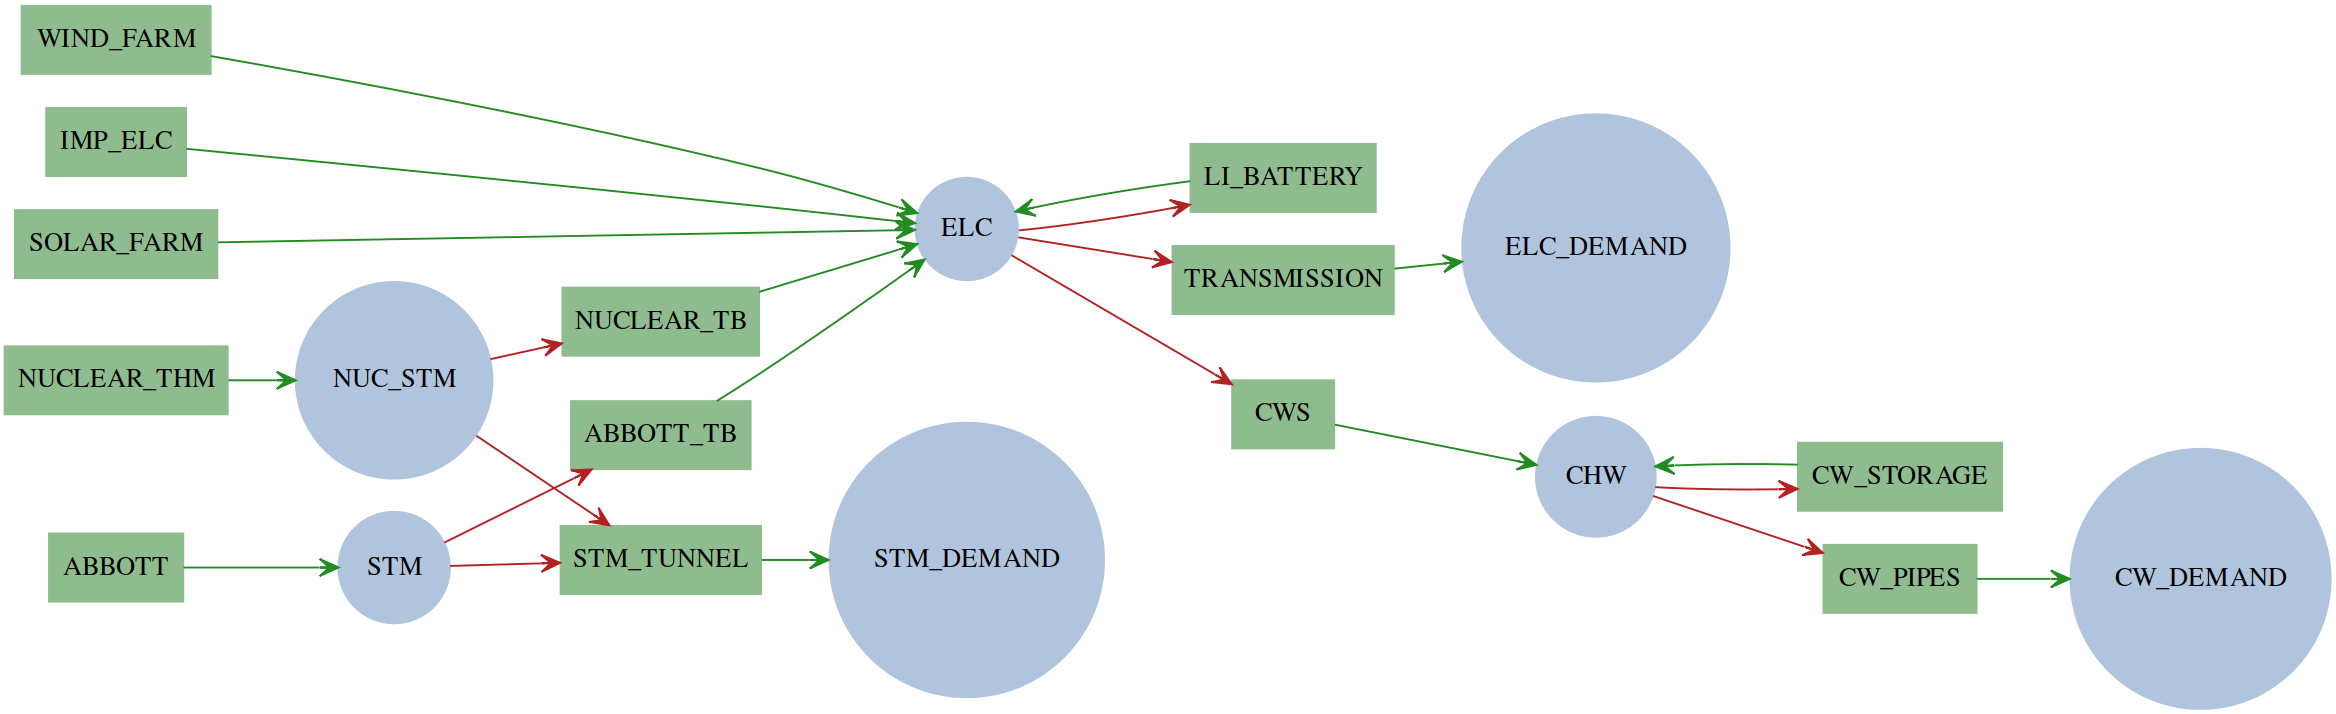
\includegraphics[width=\columnwidth]{uiuc_system.png}
  \caption{The \gls{uiuc} energy system modeled in \gls{temoa}}
  \label{fig:uiucsys}
\end{figure}

Figure \ref{fig:uiucsys} shows the topology of UIUC’s energy system, modeled in Temoa.
The UIUC model is spatially simple, since there is only one region, but topologically
more complex than the Illinois model from Section \ref{section:ilmodel} with
three interconnected end-use demands.

\subsection{Model and Data}
All campus data were obtained from the Facilities and Services Department at \gls{uiuc}.
Cost and operational data were also retrieved from the \gls{uiuc} ''Utilities
Production and Distribution Master Plan'' \cite{affiliated_engineers_inc_utilities_2015}.
Table \ref{tab:uiuc-tech} summarizes the technologies and some key parameters
used in the \gls{temoa} model. Similar to the Illinois case study, all technologies have
an ``efficiency'' of unity because fuel resources are not modeled.
I analyzed the structural uncertainty of this model using \gls{mga}, which constructs
alternative futures that are not necessarily motivated by cost. Additionally,
as a research university, \gls{uiuc} is interested in developing pre-commercial
technologies (e.g. a geothermal loop for heating and cooling). For these reasons,
the technology learning curves are not applied in the \gls{uiuc} model.

\subsubsection{Campus Steam}
\gls{uiuc} heats most of its buildings with steam generated by natural gas and
coal plant on campus, \gls{abbott}. \gls{abbott} is a combined cycle facility that
can operate in a condensing mode to capture steam to generate electricity or an
extraction mode that sends steam to campus for heating
\cite{affiliated_engineers_inc_utilities_2015}. \gls{temoa} does not have a
convenient way to model combined cycle plants \cite{decarolis_temoa_2010}. The
\gls{temoa} team suggests splitting the output of the technology. However, this
forces the \gls{abbott} model to generate steam and electricity in a fixed ratio, which
is not how \gls{abbott} operates. I circumvent this issue by introducing a dummy
technology, \texttt{ABBOTT\_TB}, that converts steam to electricity. Thus, \gls{temoa}
must choose how to use the steam produced by \gls{abbott}, matching operational reality.
I modeled an on-campus nuclear reactor in a similar manner. The nuclear reactor
generates a unique commodity, \texttt{NUC\_STM}, to distinguish nuclear activity
from \gls{abbott}'s activity.
% Figure \ref{fig:historical-steam} shows hourly steam demand from \gls{uiuc} fiscal years 2014 to 2019.

% \begin{figure}[H]
%   \centering
%   \resizebox{0.8\columnwidth}{!}{%% Creator: Matplotlib, PGF backend
%%
%% To include the figure in your LaTeX document, write
%%   \input{<filename>.pgf}
%%
%% Make sure the required packages are loaded in your preamble
%%   \usepackage{pgf}
%%
%% Figures using additional raster images can only be included by \input if
%% they are in the same directory as the main LaTeX file. For loading figures
%% from other directories you can use the `import` package
%%   \usepackage{import}
%%
%% and then include the figures with
%%   \import{<path to file>}{<filename>.pgf}
%%
%% Matplotlib used the following preamble
%%
\begingroup%
\makeatletter%
\begin{pgfpicture}%
\pgfpathrectangle{\pgfpointorigin}{\pgfqpoint{13.322565in}{6.822124in}}%
\pgfusepath{use as bounding box, clip}%
\begin{pgfscope}%
\pgfsetbuttcap%
\pgfsetmiterjoin%
\definecolor{currentfill}{rgb}{1.000000,1.000000,1.000000}%
\pgfsetfillcolor{currentfill}%
\pgfsetlinewidth{0.000000pt}%
\definecolor{currentstroke}{rgb}{0.500000,0.500000,0.500000}%
\pgfsetstrokecolor{currentstroke}%
\pgfsetdash{}{0pt}%
\pgfpathmoveto{\pgfqpoint{0.000000in}{-0.000000in}}%
\pgfpathlineto{\pgfqpoint{13.322565in}{-0.000000in}}%
\pgfpathlineto{\pgfqpoint{13.322565in}{6.822124in}}%
\pgfpathlineto{\pgfqpoint{0.000000in}{6.822124in}}%
\pgfpathclose%
\pgfusepath{fill}%
\end{pgfscope}%
\begin{pgfscope}%
\pgfsetbuttcap%
\pgfsetmiterjoin%
\definecolor{currentfill}{rgb}{0.898039,0.898039,0.898039}%
\pgfsetfillcolor{currentfill}%
\pgfsetlinewidth{0.000000pt}%
\definecolor{currentstroke}{rgb}{0.000000,0.000000,0.000000}%
\pgfsetstrokecolor{currentstroke}%
\pgfsetstrokeopacity{0.000000}%
\pgfsetdash{}{0pt}%
\pgfpathmoveto{\pgfqpoint{0.822565in}{0.602124in}}%
\pgfpathlineto{\pgfqpoint{13.222565in}{0.602124in}}%
\pgfpathlineto{\pgfqpoint{13.222565in}{6.722124in}}%
\pgfpathlineto{\pgfqpoint{0.822565in}{6.722124in}}%
\pgfpathclose%
\pgfusepath{fill}%
\end{pgfscope}%
\begin{pgfscope}%
\pgfpathrectangle{\pgfqpoint{0.822565in}{0.602124in}}{\pgfqpoint{12.400000in}{6.120000in}}%
\pgfusepath{clip}%
\pgfsetrectcap%
\pgfsetroundjoin%
\pgfsetlinewidth{0.803000pt}%
\definecolor{currentstroke}{rgb}{1.000000,1.000000,1.000000}%
\pgfsetstrokecolor{currentstroke}%
\pgfsetdash{}{0pt}%
\pgfpathmoveto{\pgfqpoint{2.522143in}{0.602124in}}%
\pgfpathlineto{\pgfqpoint{2.522143in}{6.722124in}}%
\pgfusepath{stroke}%
\end{pgfscope}%
\begin{pgfscope}%
\pgfsetbuttcap%
\pgfsetroundjoin%
\definecolor{currentfill}{rgb}{0.333333,0.333333,0.333333}%
\pgfsetfillcolor{currentfill}%
\pgfsetlinewidth{0.803000pt}%
\definecolor{currentstroke}{rgb}{0.333333,0.333333,0.333333}%
\pgfsetstrokecolor{currentstroke}%
\pgfsetdash{}{0pt}%
\pgfsys@defobject{currentmarker}{\pgfqpoint{0.000000in}{-0.048611in}}{\pgfqpoint{0.000000in}{0.000000in}}{%
\pgfpathmoveto{\pgfqpoint{0.000000in}{0.000000in}}%
\pgfpathlineto{\pgfqpoint{0.000000in}{-0.048611in}}%
\pgfusepath{stroke,fill}%
}%
\begin{pgfscope}%
\pgfsys@transformshift{2.522143in}{0.602124in}%
\pgfsys@useobject{currentmarker}{}%
\end{pgfscope}%
\end{pgfscope}%
\begin{pgfscope}%
\definecolor{textcolor}{rgb}{0.333333,0.333333,0.333333}%
\pgfsetstrokecolor{textcolor}%
\pgfsetfillcolor{textcolor}%
\pgftext[x=2.117515in, y=0.140428in, left, base,rotate=30.000000]{\color{textcolor}\rmfamily\fontsize{16.000000}{19.200000}\selectfont \(\displaystyle {2015}\)}%
\end{pgfscope}%
\begin{pgfscope}%
\pgfpathrectangle{\pgfqpoint{0.822565in}{0.602124in}}{\pgfqpoint{12.400000in}{6.120000in}}%
\pgfusepath{clip}%
\pgfsetrectcap%
\pgfsetroundjoin%
\pgfsetlinewidth{0.803000pt}%
\definecolor{currentstroke}{rgb}{1.000000,1.000000,1.000000}%
\pgfsetstrokecolor{currentstroke}%
\pgfsetdash{}{0pt}%
\pgfpathmoveto{\pgfqpoint{4.775505in}{0.602124in}}%
\pgfpathlineto{\pgfqpoint{4.775505in}{6.722124in}}%
\pgfusepath{stroke}%
\end{pgfscope}%
\begin{pgfscope}%
\pgfsetbuttcap%
\pgfsetroundjoin%
\definecolor{currentfill}{rgb}{0.333333,0.333333,0.333333}%
\pgfsetfillcolor{currentfill}%
\pgfsetlinewidth{0.803000pt}%
\definecolor{currentstroke}{rgb}{0.333333,0.333333,0.333333}%
\pgfsetstrokecolor{currentstroke}%
\pgfsetdash{}{0pt}%
\pgfsys@defobject{currentmarker}{\pgfqpoint{0.000000in}{-0.048611in}}{\pgfqpoint{0.000000in}{0.000000in}}{%
\pgfpathmoveto{\pgfqpoint{0.000000in}{0.000000in}}%
\pgfpathlineto{\pgfqpoint{0.000000in}{-0.048611in}}%
\pgfusepath{stroke,fill}%
}%
\begin{pgfscope}%
\pgfsys@transformshift{4.775505in}{0.602124in}%
\pgfsys@useobject{currentmarker}{}%
\end{pgfscope}%
\end{pgfscope}%
\begin{pgfscope}%
\definecolor{textcolor}{rgb}{0.333333,0.333333,0.333333}%
\pgfsetstrokecolor{textcolor}%
\pgfsetfillcolor{textcolor}%
\pgftext[x=4.370877in, y=0.140428in, left, base,rotate=30.000000]{\color{textcolor}\rmfamily\fontsize{16.000000}{19.200000}\selectfont \(\displaystyle {2016}\)}%
\end{pgfscope}%
\begin{pgfscope}%
\pgfpathrectangle{\pgfqpoint{0.822565in}{0.602124in}}{\pgfqpoint{12.400000in}{6.120000in}}%
\pgfusepath{clip}%
\pgfsetrectcap%
\pgfsetroundjoin%
\pgfsetlinewidth{0.803000pt}%
\definecolor{currentstroke}{rgb}{1.000000,1.000000,1.000000}%
\pgfsetstrokecolor{currentstroke}%
\pgfsetdash{}{0pt}%
\pgfpathmoveto{\pgfqpoint{7.035041in}{0.602124in}}%
\pgfpathlineto{\pgfqpoint{7.035041in}{6.722124in}}%
\pgfusepath{stroke}%
\end{pgfscope}%
\begin{pgfscope}%
\pgfsetbuttcap%
\pgfsetroundjoin%
\definecolor{currentfill}{rgb}{0.333333,0.333333,0.333333}%
\pgfsetfillcolor{currentfill}%
\pgfsetlinewidth{0.803000pt}%
\definecolor{currentstroke}{rgb}{0.333333,0.333333,0.333333}%
\pgfsetstrokecolor{currentstroke}%
\pgfsetdash{}{0pt}%
\pgfsys@defobject{currentmarker}{\pgfqpoint{0.000000in}{-0.048611in}}{\pgfqpoint{0.000000in}{0.000000in}}{%
\pgfpathmoveto{\pgfqpoint{0.000000in}{0.000000in}}%
\pgfpathlineto{\pgfqpoint{0.000000in}{-0.048611in}}%
\pgfusepath{stroke,fill}%
}%
\begin{pgfscope}%
\pgfsys@transformshift{7.035041in}{0.602124in}%
\pgfsys@useobject{currentmarker}{}%
\end{pgfscope}%
\end{pgfscope}%
\begin{pgfscope}%
\definecolor{textcolor}{rgb}{0.333333,0.333333,0.333333}%
\pgfsetstrokecolor{textcolor}%
\pgfsetfillcolor{textcolor}%
\pgftext[x=6.630413in, y=0.140428in, left, base,rotate=30.000000]{\color{textcolor}\rmfamily\fontsize{16.000000}{19.200000}\selectfont \(\displaystyle {2017}\)}%
\end{pgfscope}%
\begin{pgfscope}%
\pgfpathrectangle{\pgfqpoint{0.822565in}{0.602124in}}{\pgfqpoint{12.400000in}{6.120000in}}%
\pgfusepath{clip}%
\pgfsetrectcap%
\pgfsetroundjoin%
\pgfsetlinewidth{0.803000pt}%
\definecolor{currentstroke}{rgb}{1.000000,1.000000,1.000000}%
\pgfsetstrokecolor{currentstroke}%
\pgfsetdash{}{0pt}%
\pgfpathmoveto{\pgfqpoint{9.288403in}{0.602124in}}%
\pgfpathlineto{\pgfqpoint{9.288403in}{6.722124in}}%
\pgfusepath{stroke}%
\end{pgfscope}%
\begin{pgfscope}%
\pgfsetbuttcap%
\pgfsetroundjoin%
\definecolor{currentfill}{rgb}{0.333333,0.333333,0.333333}%
\pgfsetfillcolor{currentfill}%
\pgfsetlinewidth{0.803000pt}%
\definecolor{currentstroke}{rgb}{0.333333,0.333333,0.333333}%
\pgfsetstrokecolor{currentstroke}%
\pgfsetdash{}{0pt}%
\pgfsys@defobject{currentmarker}{\pgfqpoint{0.000000in}{-0.048611in}}{\pgfqpoint{0.000000in}{0.000000in}}{%
\pgfpathmoveto{\pgfqpoint{0.000000in}{0.000000in}}%
\pgfpathlineto{\pgfqpoint{0.000000in}{-0.048611in}}%
\pgfusepath{stroke,fill}%
}%
\begin{pgfscope}%
\pgfsys@transformshift{9.288403in}{0.602124in}%
\pgfsys@useobject{currentmarker}{}%
\end{pgfscope}%
\end{pgfscope}%
\begin{pgfscope}%
\definecolor{textcolor}{rgb}{0.333333,0.333333,0.333333}%
\pgfsetstrokecolor{textcolor}%
\pgfsetfillcolor{textcolor}%
\pgftext[x=8.883775in, y=0.140428in, left, base,rotate=30.000000]{\color{textcolor}\rmfamily\fontsize{16.000000}{19.200000}\selectfont \(\displaystyle {2018}\)}%
\end{pgfscope}%
\begin{pgfscope}%
\pgfpathrectangle{\pgfqpoint{0.822565in}{0.602124in}}{\pgfqpoint{12.400000in}{6.120000in}}%
\pgfusepath{clip}%
\pgfsetrectcap%
\pgfsetroundjoin%
\pgfsetlinewidth{0.803000pt}%
\definecolor{currentstroke}{rgb}{1.000000,1.000000,1.000000}%
\pgfsetstrokecolor{currentstroke}%
\pgfsetdash{}{0pt}%
\pgfpathmoveto{\pgfqpoint{11.541765in}{0.602124in}}%
\pgfpathlineto{\pgfqpoint{11.541765in}{6.722124in}}%
\pgfusepath{stroke}%
\end{pgfscope}%
\begin{pgfscope}%
\pgfsetbuttcap%
\pgfsetroundjoin%
\definecolor{currentfill}{rgb}{0.333333,0.333333,0.333333}%
\pgfsetfillcolor{currentfill}%
\pgfsetlinewidth{0.803000pt}%
\definecolor{currentstroke}{rgb}{0.333333,0.333333,0.333333}%
\pgfsetstrokecolor{currentstroke}%
\pgfsetdash{}{0pt}%
\pgfsys@defobject{currentmarker}{\pgfqpoint{0.000000in}{-0.048611in}}{\pgfqpoint{0.000000in}{0.000000in}}{%
\pgfpathmoveto{\pgfqpoint{0.000000in}{0.000000in}}%
\pgfpathlineto{\pgfqpoint{0.000000in}{-0.048611in}}%
\pgfusepath{stroke,fill}%
}%
\begin{pgfscope}%
\pgfsys@transformshift{11.541765in}{0.602124in}%
\pgfsys@useobject{currentmarker}{}%
\end{pgfscope}%
\end{pgfscope}%
\begin{pgfscope}%
\definecolor{textcolor}{rgb}{0.333333,0.333333,0.333333}%
\pgfsetstrokecolor{textcolor}%
\pgfsetfillcolor{textcolor}%
\pgftext[x=11.137137in, y=0.140428in, left, base,rotate=30.000000]{\color{textcolor}\rmfamily\fontsize{16.000000}{19.200000}\selectfont \(\displaystyle {2019}\)}%
\end{pgfscope}%
\begin{pgfscope}%
\pgfsetbuttcap%
\pgfsetroundjoin%
\definecolor{currentfill}{rgb}{0.333333,0.333333,0.333333}%
\pgfsetfillcolor{currentfill}%
\pgfsetlinewidth{0.602250pt}%
\definecolor{currentstroke}{rgb}{0.333333,0.333333,0.333333}%
\pgfsetstrokecolor{currentstroke}%
\pgfsetdash{}{0pt}%
\pgfsys@defobject{currentmarker}{\pgfqpoint{0.000000in}{-0.027778in}}{\pgfqpoint{0.000000in}{0.000000in}}{%
\pgfpathmoveto{\pgfqpoint{0.000000in}{0.000000in}}%
\pgfpathlineto{\pgfqpoint{0.000000in}{-0.027778in}}%
\pgfusepath{stroke,fill}%
}%
\begin{pgfscope}%
\pgfsys@transformshift{0.832121in}{0.602124in}%
\pgfsys@useobject{currentmarker}{}%
\end{pgfscope}%
\end{pgfscope}%
\begin{pgfscope}%
\pgfsetbuttcap%
\pgfsetroundjoin%
\definecolor{currentfill}{rgb}{0.333333,0.333333,0.333333}%
\pgfsetfillcolor{currentfill}%
\pgfsetlinewidth{0.602250pt}%
\definecolor{currentstroke}{rgb}{0.333333,0.333333,0.333333}%
\pgfsetstrokecolor{currentstroke}%
\pgfsetdash{}{0pt}%
\pgfsys@defobject{currentmarker}{\pgfqpoint{0.000000in}{-0.027778in}}{\pgfqpoint{0.000000in}{0.000000in}}{%
\pgfpathmoveto{\pgfqpoint{0.000000in}{0.000000in}}%
\pgfpathlineto{\pgfqpoint{0.000000in}{-0.027778in}}%
\pgfusepath{stroke,fill}%
}%
\begin{pgfscope}%
\pgfsys@transformshift{1.395462in}{0.602124in}%
\pgfsys@useobject{currentmarker}{}%
\end{pgfscope}%
\end{pgfscope}%
\begin{pgfscope}%
\pgfsetbuttcap%
\pgfsetroundjoin%
\definecolor{currentfill}{rgb}{0.333333,0.333333,0.333333}%
\pgfsetfillcolor{currentfill}%
\pgfsetlinewidth{0.602250pt}%
\definecolor{currentstroke}{rgb}{0.333333,0.333333,0.333333}%
\pgfsetstrokecolor{currentstroke}%
\pgfsetdash{}{0pt}%
\pgfsys@defobject{currentmarker}{\pgfqpoint{0.000000in}{-0.027778in}}{\pgfqpoint{0.000000in}{0.000000in}}{%
\pgfpathmoveto{\pgfqpoint{0.000000in}{0.000000in}}%
\pgfpathlineto{\pgfqpoint{0.000000in}{-0.027778in}}%
\pgfusepath{stroke,fill}%
}%
\begin{pgfscope}%
\pgfsys@transformshift{1.958803in}{0.602124in}%
\pgfsys@useobject{currentmarker}{}%
\end{pgfscope}%
\end{pgfscope}%
\begin{pgfscope}%
\pgfsetbuttcap%
\pgfsetroundjoin%
\definecolor{currentfill}{rgb}{0.333333,0.333333,0.333333}%
\pgfsetfillcolor{currentfill}%
\pgfsetlinewidth{0.602250pt}%
\definecolor{currentstroke}{rgb}{0.333333,0.333333,0.333333}%
\pgfsetstrokecolor{currentstroke}%
\pgfsetdash{}{0pt}%
\pgfsys@defobject{currentmarker}{\pgfqpoint{0.000000in}{-0.027778in}}{\pgfqpoint{0.000000in}{0.000000in}}{%
\pgfpathmoveto{\pgfqpoint{0.000000in}{0.000000in}}%
\pgfpathlineto{\pgfqpoint{0.000000in}{-0.027778in}}%
\pgfusepath{stroke,fill}%
}%
\begin{pgfscope}%
\pgfsys@transformshift{3.085484in}{0.602124in}%
\pgfsys@useobject{currentmarker}{}%
\end{pgfscope}%
\end{pgfscope}%
\begin{pgfscope}%
\pgfsetbuttcap%
\pgfsetroundjoin%
\definecolor{currentfill}{rgb}{0.333333,0.333333,0.333333}%
\pgfsetfillcolor{currentfill}%
\pgfsetlinewidth{0.602250pt}%
\definecolor{currentstroke}{rgb}{0.333333,0.333333,0.333333}%
\pgfsetstrokecolor{currentstroke}%
\pgfsetdash{}{0pt}%
\pgfsys@defobject{currentmarker}{\pgfqpoint{0.000000in}{-0.027778in}}{\pgfqpoint{0.000000in}{0.000000in}}{%
\pgfpathmoveto{\pgfqpoint{0.000000in}{0.000000in}}%
\pgfpathlineto{\pgfqpoint{0.000000in}{-0.027778in}}%
\pgfusepath{stroke,fill}%
}%
\begin{pgfscope}%
\pgfsys@transformshift{3.648824in}{0.602124in}%
\pgfsys@useobject{currentmarker}{}%
\end{pgfscope}%
\end{pgfscope}%
\begin{pgfscope}%
\pgfsetbuttcap%
\pgfsetroundjoin%
\definecolor{currentfill}{rgb}{0.333333,0.333333,0.333333}%
\pgfsetfillcolor{currentfill}%
\pgfsetlinewidth{0.602250pt}%
\definecolor{currentstroke}{rgb}{0.333333,0.333333,0.333333}%
\pgfsetstrokecolor{currentstroke}%
\pgfsetdash{}{0pt}%
\pgfsys@defobject{currentmarker}{\pgfqpoint{0.000000in}{-0.027778in}}{\pgfqpoint{0.000000in}{0.000000in}}{%
\pgfpathmoveto{\pgfqpoint{0.000000in}{0.000000in}}%
\pgfpathlineto{\pgfqpoint{0.000000in}{-0.027778in}}%
\pgfusepath{stroke,fill}%
}%
\begin{pgfscope}%
\pgfsys@transformshift{4.212165in}{0.602124in}%
\pgfsys@useobject{currentmarker}{}%
\end{pgfscope}%
\end{pgfscope}%
\begin{pgfscope}%
\pgfsetbuttcap%
\pgfsetroundjoin%
\definecolor{currentfill}{rgb}{0.333333,0.333333,0.333333}%
\pgfsetfillcolor{currentfill}%
\pgfsetlinewidth{0.602250pt}%
\definecolor{currentstroke}{rgb}{0.333333,0.333333,0.333333}%
\pgfsetstrokecolor{currentstroke}%
\pgfsetdash{}{0pt}%
\pgfsys@defobject{currentmarker}{\pgfqpoint{0.000000in}{-0.027778in}}{\pgfqpoint{0.000000in}{0.000000in}}{%
\pgfpathmoveto{\pgfqpoint{0.000000in}{0.000000in}}%
\pgfpathlineto{\pgfqpoint{0.000000in}{-0.027778in}}%
\pgfusepath{stroke,fill}%
}%
\begin{pgfscope}%
\pgfsys@transformshift{5.338846in}{0.602124in}%
\pgfsys@useobject{currentmarker}{}%
\end{pgfscope}%
\end{pgfscope}%
\begin{pgfscope}%
\pgfsetbuttcap%
\pgfsetroundjoin%
\definecolor{currentfill}{rgb}{0.333333,0.333333,0.333333}%
\pgfsetfillcolor{currentfill}%
\pgfsetlinewidth{0.602250pt}%
\definecolor{currentstroke}{rgb}{0.333333,0.333333,0.333333}%
\pgfsetstrokecolor{currentstroke}%
\pgfsetdash{}{0pt}%
\pgfsys@defobject{currentmarker}{\pgfqpoint{0.000000in}{-0.027778in}}{\pgfqpoint{0.000000in}{0.000000in}}{%
\pgfpathmoveto{\pgfqpoint{0.000000in}{0.000000in}}%
\pgfpathlineto{\pgfqpoint{0.000000in}{-0.027778in}}%
\pgfusepath{stroke,fill}%
}%
\begin{pgfscope}%
\pgfsys@transformshift{5.902186in}{0.602124in}%
\pgfsys@useobject{currentmarker}{}%
\end{pgfscope}%
\end{pgfscope}%
\begin{pgfscope}%
\pgfsetbuttcap%
\pgfsetroundjoin%
\definecolor{currentfill}{rgb}{0.333333,0.333333,0.333333}%
\pgfsetfillcolor{currentfill}%
\pgfsetlinewidth{0.602250pt}%
\definecolor{currentstroke}{rgb}{0.333333,0.333333,0.333333}%
\pgfsetstrokecolor{currentstroke}%
\pgfsetdash{}{0pt}%
\pgfsys@defobject{currentmarker}{\pgfqpoint{0.000000in}{-0.027778in}}{\pgfqpoint{0.000000in}{0.000000in}}{%
\pgfpathmoveto{\pgfqpoint{0.000000in}{0.000000in}}%
\pgfpathlineto{\pgfqpoint{0.000000in}{-0.027778in}}%
\pgfusepath{stroke,fill}%
}%
\begin{pgfscope}%
\pgfsys@transformshift{6.465527in}{0.602124in}%
\pgfsys@useobject{currentmarker}{}%
\end{pgfscope}%
\end{pgfscope}%
\begin{pgfscope}%
\pgfsetbuttcap%
\pgfsetroundjoin%
\definecolor{currentfill}{rgb}{0.333333,0.333333,0.333333}%
\pgfsetfillcolor{currentfill}%
\pgfsetlinewidth{0.602250pt}%
\definecolor{currentstroke}{rgb}{0.333333,0.333333,0.333333}%
\pgfsetstrokecolor{currentstroke}%
\pgfsetdash{}{0pt}%
\pgfsys@defobject{currentmarker}{\pgfqpoint{0.000000in}{-0.027778in}}{\pgfqpoint{0.000000in}{0.000000in}}{%
\pgfpathmoveto{\pgfqpoint{0.000000in}{0.000000in}}%
\pgfpathlineto{\pgfqpoint{0.000000in}{-0.027778in}}%
\pgfusepath{stroke,fill}%
}%
\begin{pgfscope}%
\pgfsys@transformshift{7.028867in}{0.602124in}%
\pgfsys@useobject{currentmarker}{}%
\end{pgfscope}%
\end{pgfscope}%
\begin{pgfscope}%
\pgfsetbuttcap%
\pgfsetroundjoin%
\definecolor{currentfill}{rgb}{0.333333,0.333333,0.333333}%
\pgfsetfillcolor{currentfill}%
\pgfsetlinewidth{0.602250pt}%
\definecolor{currentstroke}{rgb}{0.333333,0.333333,0.333333}%
\pgfsetstrokecolor{currentstroke}%
\pgfsetdash{}{0pt}%
\pgfsys@defobject{currentmarker}{\pgfqpoint{0.000000in}{-0.027778in}}{\pgfqpoint{0.000000in}{0.000000in}}{%
\pgfpathmoveto{\pgfqpoint{0.000000in}{0.000000in}}%
\pgfpathlineto{\pgfqpoint{0.000000in}{-0.027778in}}%
\pgfusepath{stroke,fill}%
}%
\begin{pgfscope}%
\pgfsys@transformshift{7.592208in}{0.602124in}%
\pgfsys@useobject{currentmarker}{}%
\end{pgfscope}%
\end{pgfscope}%
\begin{pgfscope}%
\pgfsetbuttcap%
\pgfsetroundjoin%
\definecolor{currentfill}{rgb}{0.333333,0.333333,0.333333}%
\pgfsetfillcolor{currentfill}%
\pgfsetlinewidth{0.602250pt}%
\definecolor{currentstroke}{rgb}{0.333333,0.333333,0.333333}%
\pgfsetstrokecolor{currentstroke}%
\pgfsetdash{}{0pt}%
\pgfsys@defobject{currentmarker}{\pgfqpoint{0.000000in}{-0.027778in}}{\pgfqpoint{0.000000in}{0.000000in}}{%
\pgfpathmoveto{\pgfqpoint{0.000000in}{0.000000in}}%
\pgfpathlineto{\pgfqpoint{0.000000in}{-0.027778in}}%
\pgfusepath{stroke,fill}%
}%
\begin{pgfscope}%
\pgfsys@transformshift{8.155549in}{0.602124in}%
\pgfsys@useobject{currentmarker}{}%
\end{pgfscope}%
\end{pgfscope}%
\begin{pgfscope}%
\pgfsetbuttcap%
\pgfsetroundjoin%
\definecolor{currentfill}{rgb}{0.333333,0.333333,0.333333}%
\pgfsetfillcolor{currentfill}%
\pgfsetlinewidth{0.602250pt}%
\definecolor{currentstroke}{rgb}{0.333333,0.333333,0.333333}%
\pgfsetstrokecolor{currentstroke}%
\pgfsetdash{}{0pt}%
\pgfsys@defobject{currentmarker}{\pgfqpoint{0.000000in}{-0.027778in}}{\pgfqpoint{0.000000in}{0.000000in}}{%
\pgfpathmoveto{\pgfqpoint{0.000000in}{0.000000in}}%
\pgfpathlineto{\pgfqpoint{0.000000in}{-0.027778in}}%
\pgfusepath{stroke,fill}%
}%
\begin{pgfscope}%
\pgfsys@transformshift{8.718889in}{0.602124in}%
\pgfsys@useobject{currentmarker}{}%
\end{pgfscope}%
\end{pgfscope}%
\begin{pgfscope}%
\pgfsetbuttcap%
\pgfsetroundjoin%
\definecolor{currentfill}{rgb}{0.333333,0.333333,0.333333}%
\pgfsetfillcolor{currentfill}%
\pgfsetlinewidth{0.602250pt}%
\definecolor{currentstroke}{rgb}{0.333333,0.333333,0.333333}%
\pgfsetstrokecolor{currentstroke}%
\pgfsetdash{}{0pt}%
\pgfsys@defobject{currentmarker}{\pgfqpoint{0.000000in}{-0.027778in}}{\pgfqpoint{0.000000in}{0.000000in}}{%
\pgfpathmoveto{\pgfqpoint{0.000000in}{0.000000in}}%
\pgfpathlineto{\pgfqpoint{0.000000in}{-0.027778in}}%
\pgfusepath{stroke,fill}%
}%
\begin{pgfscope}%
\pgfsys@transformshift{9.282230in}{0.602124in}%
\pgfsys@useobject{currentmarker}{}%
\end{pgfscope}%
\end{pgfscope}%
\begin{pgfscope}%
\pgfsetbuttcap%
\pgfsetroundjoin%
\definecolor{currentfill}{rgb}{0.333333,0.333333,0.333333}%
\pgfsetfillcolor{currentfill}%
\pgfsetlinewidth{0.602250pt}%
\definecolor{currentstroke}{rgb}{0.333333,0.333333,0.333333}%
\pgfsetstrokecolor{currentstroke}%
\pgfsetdash{}{0pt}%
\pgfsys@defobject{currentmarker}{\pgfqpoint{0.000000in}{-0.027778in}}{\pgfqpoint{0.000000in}{0.000000in}}{%
\pgfpathmoveto{\pgfqpoint{0.000000in}{0.000000in}}%
\pgfpathlineto{\pgfqpoint{0.000000in}{-0.027778in}}%
\pgfusepath{stroke,fill}%
}%
\begin{pgfscope}%
\pgfsys@transformshift{9.845570in}{0.602124in}%
\pgfsys@useobject{currentmarker}{}%
\end{pgfscope}%
\end{pgfscope}%
\begin{pgfscope}%
\pgfsetbuttcap%
\pgfsetroundjoin%
\definecolor{currentfill}{rgb}{0.333333,0.333333,0.333333}%
\pgfsetfillcolor{currentfill}%
\pgfsetlinewidth{0.602250pt}%
\definecolor{currentstroke}{rgb}{0.333333,0.333333,0.333333}%
\pgfsetstrokecolor{currentstroke}%
\pgfsetdash{}{0pt}%
\pgfsys@defobject{currentmarker}{\pgfqpoint{0.000000in}{-0.027778in}}{\pgfqpoint{0.000000in}{0.000000in}}{%
\pgfpathmoveto{\pgfqpoint{0.000000in}{0.000000in}}%
\pgfpathlineto{\pgfqpoint{0.000000in}{-0.027778in}}%
\pgfusepath{stroke,fill}%
}%
\begin{pgfscope}%
\pgfsys@transformshift{10.408911in}{0.602124in}%
\pgfsys@useobject{currentmarker}{}%
\end{pgfscope}%
\end{pgfscope}%
\begin{pgfscope}%
\pgfsetbuttcap%
\pgfsetroundjoin%
\definecolor{currentfill}{rgb}{0.333333,0.333333,0.333333}%
\pgfsetfillcolor{currentfill}%
\pgfsetlinewidth{0.602250pt}%
\definecolor{currentstroke}{rgb}{0.333333,0.333333,0.333333}%
\pgfsetstrokecolor{currentstroke}%
\pgfsetdash{}{0pt}%
\pgfsys@defobject{currentmarker}{\pgfqpoint{0.000000in}{-0.027778in}}{\pgfqpoint{0.000000in}{0.000000in}}{%
\pgfpathmoveto{\pgfqpoint{0.000000in}{0.000000in}}%
\pgfpathlineto{\pgfqpoint{0.000000in}{-0.027778in}}%
\pgfusepath{stroke,fill}%
}%
\begin{pgfscope}%
\pgfsys@transformshift{10.972251in}{0.602124in}%
\pgfsys@useobject{currentmarker}{}%
\end{pgfscope}%
\end{pgfscope}%
\begin{pgfscope}%
\pgfsetbuttcap%
\pgfsetroundjoin%
\definecolor{currentfill}{rgb}{0.333333,0.333333,0.333333}%
\pgfsetfillcolor{currentfill}%
\pgfsetlinewidth{0.602250pt}%
\definecolor{currentstroke}{rgb}{0.333333,0.333333,0.333333}%
\pgfsetstrokecolor{currentstroke}%
\pgfsetdash{}{0pt}%
\pgfsys@defobject{currentmarker}{\pgfqpoint{0.000000in}{-0.027778in}}{\pgfqpoint{0.000000in}{0.000000in}}{%
\pgfpathmoveto{\pgfqpoint{0.000000in}{0.000000in}}%
\pgfpathlineto{\pgfqpoint{0.000000in}{-0.027778in}}%
\pgfusepath{stroke,fill}%
}%
\begin{pgfscope}%
\pgfsys@transformshift{11.535592in}{0.602124in}%
\pgfsys@useobject{currentmarker}{}%
\end{pgfscope}%
\end{pgfscope}%
\begin{pgfscope}%
\pgfsetbuttcap%
\pgfsetroundjoin%
\definecolor{currentfill}{rgb}{0.333333,0.333333,0.333333}%
\pgfsetfillcolor{currentfill}%
\pgfsetlinewidth{0.602250pt}%
\definecolor{currentstroke}{rgb}{0.333333,0.333333,0.333333}%
\pgfsetstrokecolor{currentstroke}%
\pgfsetdash{}{0pt}%
\pgfsys@defobject{currentmarker}{\pgfqpoint{0.000000in}{-0.027778in}}{\pgfqpoint{0.000000in}{0.000000in}}{%
\pgfpathmoveto{\pgfqpoint{0.000000in}{0.000000in}}%
\pgfpathlineto{\pgfqpoint{0.000000in}{-0.027778in}}%
\pgfusepath{stroke,fill}%
}%
\begin{pgfscope}%
\pgfsys@transformshift{12.098932in}{0.602124in}%
\pgfsys@useobject{currentmarker}{}%
\end{pgfscope}%
\end{pgfscope}%
\begin{pgfscope}%
\pgfsetbuttcap%
\pgfsetroundjoin%
\definecolor{currentfill}{rgb}{0.333333,0.333333,0.333333}%
\pgfsetfillcolor{currentfill}%
\pgfsetlinewidth{0.602250pt}%
\definecolor{currentstroke}{rgb}{0.333333,0.333333,0.333333}%
\pgfsetstrokecolor{currentstroke}%
\pgfsetdash{}{0pt}%
\pgfsys@defobject{currentmarker}{\pgfqpoint{0.000000in}{-0.027778in}}{\pgfqpoint{0.000000in}{0.000000in}}{%
\pgfpathmoveto{\pgfqpoint{0.000000in}{0.000000in}}%
\pgfpathlineto{\pgfqpoint{0.000000in}{-0.027778in}}%
\pgfusepath{stroke,fill}%
}%
\begin{pgfscope}%
\pgfsys@transformshift{12.662273in}{0.602124in}%
\pgfsys@useobject{currentmarker}{}%
\end{pgfscope}%
\end{pgfscope}%
\begin{pgfscope}%
\pgfpathrectangle{\pgfqpoint{0.822565in}{0.602124in}}{\pgfqpoint{12.400000in}{6.120000in}}%
\pgfusepath{clip}%
\pgfsetrectcap%
\pgfsetroundjoin%
\pgfsetlinewidth{0.803000pt}%
\definecolor{currentstroke}{rgb}{1.000000,1.000000,1.000000}%
\pgfsetstrokecolor{currentstroke}%
\pgfsetdash{}{0pt}%
\pgfpathmoveto{\pgfqpoint{0.822565in}{0.880306in}}%
\pgfpathlineto{\pgfqpoint{13.222565in}{0.880306in}}%
\pgfusepath{stroke}%
\end{pgfscope}%
\begin{pgfscope}%
\pgfsetbuttcap%
\pgfsetroundjoin%
\definecolor{currentfill}{rgb}{0.333333,0.333333,0.333333}%
\pgfsetfillcolor{currentfill}%
\pgfsetlinewidth{0.803000pt}%
\definecolor{currentstroke}{rgb}{0.333333,0.333333,0.333333}%
\pgfsetstrokecolor{currentstroke}%
\pgfsetdash{}{0pt}%
\pgfsys@defobject{currentmarker}{\pgfqpoint{-0.048611in}{0.000000in}}{\pgfqpoint{-0.000000in}{0.000000in}}{%
\pgfpathmoveto{\pgfqpoint{-0.000000in}{0.000000in}}%
\pgfpathlineto{\pgfqpoint{-0.048611in}{0.000000in}}%
\pgfusepath{stroke,fill}%
}%
\begin{pgfscope}%
\pgfsys@transformshift{0.822565in}{0.880306in}%
\pgfsys@useobject{currentmarker}{}%
\end{pgfscope}%
\end{pgfscope}%
\begin{pgfscope}%
\definecolor{textcolor}{rgb}{0.333333,0.333333,0.333333}%
\pgfsetstrokecolor{textcolor}%
\pgfsetfillcolor{textcolor}%
\pgftext[x=0.615275in, y=0.796972in, left, base]{\color{textcolor}\rmfamily\fontsize{16.000000}{19.200000}\selectfont \(\displaystyle {0}\)}%
\end{pgfscope}%
\begin{pgfscope}%
\pgfpathrectangle{\pgfqpoint{0.822565in}{0.602124in}}{\pgfqpoint{12.400000in}{6.120000in}}%
\pgfusepath{clip}%
\pgfsetrectcap%
\pgfsetroundjoin%
\pgfsetlinewidth{0.803000pt}%
\definecolor{currentstroke}{rgb}{1.000000,1.000000,1.000000}%
\pgfsetstrokecolor{currentstroke}%
\pgfsetdash{}{0pt}%
\pgfpathmoveto{\pgfqpoint{0.822565in}{2.119171in}}%
\pgfpathlineto{\pgfqpoint{13.222565in}{2.119171in}}%
\pgfusepath{stroke}%
\end{pgfscope}%
\begin{pgfscope}%
\pgfsetbuttcap%
\pgfsetroundjoin%
\definecolor{currentfill}{rgb}{0.333333,0.333333,0.333333}%
\pgfsetfillcolor{currentfill}%
\pgfsetlinewidth{0.803000pt}%
\definecolor{currentstroke}{rgb}{0.333333,0.333333,0.333333}%
\pgfsetstrokecolor{currentstroke}%
\pgfsetdash{}{0pt}%
\pgfsys@defobject{currentmarker}{\pgfqpoint{-0.048611in}{0.000000in}}{\pgfqpoint{-0.000000in}{0.000000in}}{%
\pgfpathmoveto{\pgfqpoint{-0.000000in}{0.000000in}}%
\pgfpathlineto{\pgfqpoint{-0.048611in}{0.000000in}}%
\pgfusepath{stroke,fill}%
}%
\begin{pgfscope}%
\pgfsys@transformshift{0.822565in}{2.119171in}%
\pgfsys@useobject{currentmarker}{}%
\end{pgfscope}%
\end{pgfscope}%
\begin{pgfscope}%
\definecolor{textcolor}{rgb}{0.333333,0.333333,0.333333}%
\pgfsetstrokecolor{textcolor}%
\pgfsetfillcolor{textcolor}%
\pgftext[x=0.505207in, y=2.035838in, left, base]{\color{textcolor}\rmfamily\fontsize{16.000000}{19.200000}\selectfont \(\displaystyle {50}\)}%
\end{pgfscope}%
\begin{pgfscope}%
\pgfpathrectangle{\pgfqpoint{0.822565in}{0.602124in}}{\pgfqpoint{12.400000in}{6.120000in}}%
\pgfusepath{clip}%
\pgfsetrectcap%
\pgfsetroundjoin%
\pgfsetlinewidth{0.803000pt}%
\definecolor{currentstroke}{rgb}{1.000000,1.000000,1.000000}%
\pgfsetstrokecolor{currentstroke}%
\pgfsetdash{}{0pt}%
\pgfpathmoveto{\pgfqpoint{0.822565in}{3.358037in}}%
\pgfpathlineto{\pgfqpoint{13.222565in}{3.358037in}}%
\pgfusepath{stroke}%
\end{pgfscope}%
\begin{pgfscope}%
\pgfsetbuttcap%
\pgfsetroundjoin%
\definecolor{currentfill}{rgb}{0.333333,0.333333,0.333333}%
\pgfsetfillcolor{currentfill}%
\pgfsetlinewidth{0.803000pt}%
\definecolor{currentstroke}{rgb}{0.333333,0.333333,0.333333}%
\pgfsetstrokecolor{currentstroke}%
\pgfsetdash{}{0pt}%
\pgfsys@defobject{currentmarker}{\pgfqpoint{-0.048611in}{0.000000in}}{\pgfqpoint{-0.000000in}{0.000000in}}{%
\pgfpathmoveto{\pgfqpoint{-0.000000in}{0.000000in}}%
\pgfpathlineto{\pgfqpoint{-0.048611in}{0.000000in}}%
\pgfusepath{stroke,fill}%
}%
\begin{pgfscope}%
\pgfsys@transformshift{0.822565in}{3.358037in}%
\pgfsys@useobject{currentmarker}{}%
\end{pgfscope}%
\end{pgfscope}%
\begin{pgfscope}%
\definecolor{textcolor}{rgb}{0.333333,0.333333,0.333333}%
\pgfsetstrokecolor{textcolor}%
\pgfsetfillcolor{textcolor}%
\pgftext[x=0.395138in, y=3.274704in, left, base]{\color{textcolor}\rmfamily\fontsize{16.000000}{19.200000}\selectfont \(\displaystyle {100}\)}%
\end{pgfscope}%
\begin{pgfscope}%
\pgfpathrectangle{\pgfqpoint{0.822565in}{0.602124in}}{\pgfqpoint{12.400000in}{6.120000in}}%
\pgfusepath{clip}%
\pgfsetrectcap%
\pgfsetroundjoin%
\pgfsetlinewidth{0.803000pt}%
\definecolor{currentstroke}{rgb}{1.000000,1.000000,1.000000}%
\pgfsetstrokecolor{currentstroke}%
\pgfsetdash{}{0pt}%
\pgfpathmoveto{\pgfqpoint{0.822565in}{4.596903in}}%
\pgfpathlineto{\pgfqpoint{13.222565in}{4.596903in}}%
\pgfusepath{stroke}%
\end{pgfscope}%
\begin{pgfscope}%
\pgfsetbuttcap%
\pgfsetroundjoin%
\definecolor{currentfill}{rgb}{0.333333,0.333333,0.333333}%
\pgfsetfillcolor{currentfill}%
\pgfsetlinewidth{0.803000pt}%
\definecolor{currentstroke}{rgb}{0.333333,0.333333,0.333333}%
\pgfsetstrokecolor{currentstroke}%
\pgfsetdash{}{0pt}%
\pgfsys@defobject{currentmarker}{\pgfqpoint{-0.048611in}{0.000000in}}{\pgfqpoint{-0.000000in}{0.000000in}}{%
\pgfpathmoveto{\pgfqpoint{-0.000000in}{0.000000in}}%
\pgfpathlineto{\pgfqpoint{-0.048611in}{0.000000in}}%
\pgfusepath{stroke,fill}%
}%
\begin{pgfscope}%
\pgfsys@transformshift{0.822565in}{4.596903in}%
\pgfsys@useobject{currentmarker}{}%
\end{pgfscope}%
\end{pgfscope}%
\begin{pgfscope}%
\definecolor{textcolor}{rgb}{0.333333,0.333333,0.333333}%
\pgfsetstrokecolor{textcolor}%
\pgfsetfillcolor{textcolor}%
\pgftext[x=0.395138in, y=4.513569in, left, base]{\color{textcolor}\rmfamily\fontsize{16.000000}{19.200000}\selectfont \(\displaystyle {150}\)}%
\end{pgfscope}%
\begin{pgfscope}%
\pgfpathrectangle{\pgfqpoint{0.822565in}{0.602124in}}{\pgfqpoint{12.400000in}{6.120000in}}%
\pgfusepath{clip}%
\pgfsetrectcap%
\pgfsetroundjoin%
\pgfsetlinewidth{0.803000pt}%
\definecolor{currentstroke}{rgb}{1.000000,1.000000,1.000000}%
\pgfsetstrokecolor{currentstroke}%
\pgfsetdash{}{0pt}%
\pgfpathmoveto{\pgfqpoint{0.822565in}{5.835768in}}%
\pgfpathlineto{\pgfqpoint{13.222565in}{5.835768in}}%
\pgfusepath{stroke}%
\end{pgfscope}%
\begin{pgfscope}%
\pgfsetbuttcap%
\pgfsetroundjoin%
\definecolor{currentfill}{rgb}{0.333333,0.333333,0.333333}%
\pgfsetfillcolor{currentfill}%
\pgfsetlinewidth{0.803000pt}%
\definecolor{currentstroke}{rgb}{0.333333,0.333333,0.333333}%
\pgfsetstrokecolor{currentstroke}%
\pgfsetdash{}{0pt}%
\pgfsys@defobject{currentmarker}{\pgfqpoint{-0.048611in}{0.000000in}}{\pgfqpoint{-0.000000in}{0.000000in}}{%
\pgfpathmoveto{\pgfqpoint{-0.000000in}{0.000000in}}%
\pgfpathlineto{\pgfqpoint{-0.048611in}{0.000000in}}%
\pgfusepath{stroke,fill}%
}%
\begin{pgfscope}%
\pgfsys@transformshift{0.822565in}{5.835768in}%
\pgfsys@useobject{currentmarker}{}%
\end{pgfscope}%
\end{pgfscope}%
\begin{pgfscope}%
\definecolor{textcolor}{rgb}{0.333333,0.333333,0.333333}%
\pgfsetstrokecolor{textcolor}%
\pgfsetfillcolor{textcolor}%
\pgftext[x=0.395138in, y=5.752435in, left, base]{\color{textcolor}\rmfamily\fontsize{16.000000}{19.200000}\selectfont \(\displaystyle {200}\)}%
\end{pgfscope}%
\begin{pgfscope}%
\pgfsetbuttcap%
\pgfsetroundjoin%
\definecolor{currentfill}{rgb}{0.333333,0.333333,0.333333}%
\pgfsetfillcolor{currentfill}%
\pgfsetlinewidth{0.602250pt}%
\definecolor{currentstroke}{rgb}{0.333333,0.333333,0.333333}%
\pgfsetstrokecolor{currentstroke}%
\pgfsetdash{}{0pt}%
\pgfsys@defobject{currentmarker}{\pgfqpoint{-0.027778in}{0.000000in}}{\pgfqpoint{-0.000000in}{0.000000in}}{%
\pgfpathmoveto{\pgfqpoint{-0.000000in}{0.000000in}}%
\pgfpathlineto{\pgfqpoint{-0.027778in}{0.000000in}}%
\pgfusepath{stroke,fill}%
}%
\begin{pgfscope}%
\pgfsys@transformshift{0.822565in}{0.632533in}%
\pgfsys@useobject{currentmarker}{}%
\end{pgfscope}%
\end{pgfscope}%
\begin{pgfscope}%
\pgfsetbuttcap%
\pgfsetroundjoin%
\definecolor{currentfill}{rgb}{0.333333,0.333333,0.333333}%
\pgfsetfillcolor{currentfill}%
\pgfsetlinewidth{0.602250pt}%
\definecolor{currentstroke}{rgb}{0.333333,0.333333,0.333333}%
\pgfsetstrokecolor{currentstroke}%
\pgfsetdash{}{0pt}%
\pgfsys@defobject{currentmarker}{\pgfqpoint{-0.027778in}{0.000000in}}{\pgfqpoint{-0.000000in}{0.000000in}}{%
\pgfpathmoveto{\pgfqpoint{-0.000000in}{0.000000in}}%
\pgfpathlineto{\pgfqpoint{-0.027778in}{0.000000in}}%
\pgfusepath{stroke,fill}%
}%
\begin{pgfscope}%
\pgfsys@transformshift{0.822565in}{1.128079in}%
\pgfsys@useobject{currentmarker}{}%
\end{pgfscope}%
\end{pgfscope}%
\begin{pgfscope}%
\pgfsetbuttcap%
\pgfsetroundjoin%
\definecolor{currentfill}{rgb}{0.333333,0.333333,0.333333}%
\pgfsetfillcolor{currentfill}%
\pgfsetlinewidth{0.602250pt}%
\definecolor{currentstroke}{rgb}{0.333333,0.333333,0.333333}%
\pgfsetstrokecolor{currentstroke}%
\pgfsetdash{}{0pt}%
\pgfsys@defobject{currentmarker}{\pgfqpoint{-0.027778in}{0.000000in}}{\pgfqpoint{-0.000000in}{0.000000in}}{%
\pgfpathmoveto{\pgfqpoint{-0.000000in}{0.000000in}}%
\pgfpathlineto{\pgfqpoint{-0.027778in}{0.000000in}}%
\pgfusepath{stroke,fill}%
}%
\begin{pgfscope}%
\pgfsys@transformshift{0.822565in}{1.375852in}%
\pgfsys@useobject{currentmarker}{}%
\end{pgfscope}%
\end{pgfscope}%
\begin{pgfscope}%
\pgfsetbuttcap%
\pgfsetroundjoin%
\definecolor{currentfill}{rgb}{0.333333,0.333333,0.333333}%
\pgfsetfillcolor{currentfill}%
\pgfsetlinewidth{0.602250pt}%
\definecolor{currentstroke}{rgb}{0.333333,0.333333,0.333333}%
\pgfsetstrokecolor{currentstroke}%
\pgfsetdash{}{0pt}%
\pgfsys@defobject{currentmarker}{\pgfqpoint{-0.027778in}{0.000000in}}{\pgfqpoint{-0.000000in}{0.000000in}}{%
\pgfpathmoveto{\pgfqpoint{-0.000000in}{0.000000in}}%
\pgfpathlineto{\pgfqpoint{-0.027778in}{0.000000in}}%
\pgfusepath{stroke,fill}%
}%
\begin{pgfscope}%
\pgfsys@transformshift{0.822565in}{1.623625in}%
\pgfsys@useobject{currentmarker}{}%
\end{pgfscope}%
\end{pgfscope}%
\begin{pgfscope}%
\pgfsetbuttcap%
\pgfsetroundjoin%
\definecolor{currentfill}{rgb}{0.333333,0.333333,0.333333}%
\pgfsetfillcolor{currentfill}%
\pgfsetlinewidth{0.602250pt}%
\definecolor{currentstroke}{rgb}{0.333333,0.333333,0.333333}%
\pgfsetstrokecolor{currentstroke}%
\pgfsetdash{}{0pt}%
\pgfsys@defobject{currentmarker}{\pgfqpoint{-0.027778in}{0.000000in}}{\pgfqpoint{-0.000000in}{0.000000in}}{%
\pgfpathmoveto{\pgfqpoint{-0.000000in}{0.000000in}}%
\pgfpathlineto{\pgfqpoint{-0.027778in}{0.000000in}}%
\pgfusepath{stroke,fill}%
}%
\begin{pgfscope}%
\pgfsys@transformshift{0.822565in}{1.871398in}%
\pgfsys@useobject{currentmarker}{}%
\end{pgfscope}%
\end{pgfscope}%
\begin{pgfscope}%
\pgfsetbuttcap%
\pgfsetroundjoin%
\definecolor{currentfill}{rgb}{0.333333,0.333333,0.333333}%
\pgfsetfillcolor{currentfill}%
\pgfsetlinewidth{0.602250pt}%
\definecolor{currentstroke}{rgb}{0.333333,0.333333,0.333333}%
\pgfsetstrokecolor{currentstroke}%
\pgfsetdash{}{0pt}%
\pgfsys@defobject{currentmarker}{\pgfqpoint{-0.027778in}{0.000000in}}{\pgfqpoint{-0.000000in}{0.000000in}}{%
\pgfpathmoveto{\pgfqpoint{-0.000000in}{0.000000in}}%
\pgfpathlineto{\pgfqpoint{-0.027778in}{0.000000in}}%
\pgfusepath{stroke,fill}%
}%
\begin{pgfscope}%
\pgfsys@transformshift{0.822565in}{2.366944in}%
\pgfsys@useobject{currentmarker}{}%
\end{pgfscope}%
\end{pgfscope}%
\begin{pgfscope}%
\pgfsetbuttcap%
\pgfsetroundjoin%
\definecolor{currentfill}{rgb}{0.333333,0.333333,0.333333}%
\pgfsetfillcolor{currentfill}%
\pgfsetlinewidth{0.602250pt}%
\definecolor{currentstroke}{rgb}{0.333333,0.333333,0.333333}%
\pgfsetstrokecolor{currentstroke}%
\pgfsetdash{}{0pt}%
\pgfsys@defobject{currentmarker}{\pgfqpoint{-0.027778in}{0.000000in}}{\pgfqpoint{-0.000000in}{0.000000in}}{%
\pgfpathmoveto{\pgfqpoint{-0.000000in}{0.000000in}}%
\pgfpathlineto{\pgfqpoint{-0.027778in}{0.000000in}}%
\pgfusepath{stroke,fill}%
}%
\begin{pgfscope}%
\pgfsys@transformshift{0.822565in}{2.614718in}%
\pgfsys@useobject{currentmarker}{}%
\end{pgfscope}%
\end{pgfscope}%
\begin{pgfscope}%
\pgfsetbuttcap%
\pgfsetroundjoin%
\definecolor{currentfill}{rgb}{0.333333,0.333333,0.333333}%
\pgfsetfillcolor{currentfill}%
\pgfsetlinewidth{0.602250pt}%
\definecolor{currentstroke}{rgb}{0.333333,0.333333,0.333333}%
\pgfsetstrokecolor{currentstroke}%
\pgfsetdash{}{0pt}%
\pgfsys@defobject{currentmarker}{\pgfqpoint{-0.027778in}{0.000000in}}{\pgfqpoint{-0.000000in}{0.000000in}}{%
\pgfpathmoveto{\pgfqpoint{-0.000000in}{0.000000in}}%
\pgfpathlineto{\pgfqpoint{-0.027778in}{0.000000in}}%
\pgfusepath{stroke,fill}%
}%
\begin{pgfscope}%
\pgfsys@transformshift{0.822565in}{2.862491in}%
\pgfsys@useobject{currentmarker}{}%
\end{pgfscope}%
\end{pgfscope}%
\begin{pgfscope}%
\pgfsetbuttcap%
\pgfsetroundjoin%
\definecolor{currentfill}{rgb}{0.333333,0.333333,0.333333}%
\pgfsetfillcolor{currentfill}%
\pgfsetlinewidth{0.602250pt}%
\definecolor{currentstroke}{rgb}{0.333333,0.333333,0.333333}%
\pgfsetstrokecolor{currentstroke}%
\pgfsetdash{}{0pt}%
\pgfsys@defobject{currentmarker}{\pgfqpoint{-0.027778in}{0.000000in}}{\pgfqpoint{-0.000000in}{0.000000in}}{%
\pgfpathmoveto{\pgfqpoint{-0.000000in}{0.000000in}}%
\pgfpathlineto{\pgfqpoint{-0.027778in}{0.000000in}}%
\pgfusepath{stroke,fill}%
}%
\begin{pgfscope}%
\pgfsys@transformshift{0.822565in}{3.110264in}%
\pgfsys@useobject{currentmarker}{}%
\end{pgfscope}%
\end{pgfscope}%
\begin{pgfscope}%
\pgfsetbuttcap%
\pgfsetroundjoin%
\definecolor{currentfill}{rgb}{0.333333,0.333333,0.333333}%
\pgfsetfillcolor{currentfill}%
\pgfsetlinewidth{0.602250pt}%
\definecolor{currentstroke}{rgb}{0.333333,0.333333,0.333333}%
\pgfsetstrokecolor{currentstroke}%
\pgfsetdash{}{0pt}%
\pgfsys@defobject{currentmarker}{\pgfqpoint{-0.027778in}{0.000000in}}{\pgfqpoint{-0.000000in}{0.000000in}}{%
\pgfpathmoveto{\pgfqpoint{-0.000000in}{0.000000in}}%
\pgfpathlineto{\pgfqpoint{-0.027778in}{0.000000in}}%
\pgfusepath{stroke,fill}%
}%
\begin{pgfscope}%
\pgfsys@transformshift{0.822565in}{3.605810in}%
\pgfsys@useobject{currentmarker}{}%
\end{pgfscope}%
\end{pgfscope}%
\begin{pgfscope}%
\pgfsetbuttcap%
\pgfsetroundjoin%
\definecolor{currentfill}{rgb}{0.333333,0.333333,0.333333}%
\pgfsetfillcolor{currentfill}%
\pgfsetlinewidth{0.602250pt}%
\definecolor{currentstroke}{rgb}{0.333333,0.333333,0.333333}%
\pgfsetstrokecolor{currentstroke}%
\pgfsetdash{}{0pt}%
\pgfsys@defobject{currentmarker}{\pgfqpoint{-0.027778in}{0.000000in}}{\pgfqpoint{-0.000000in}{0.000000in}}{%
\pgfpathmoveto{\pgfqpoint{-0.000000in}{0.000000in}}%
\pgfpathlineto{\pgfqpoint{-0.027778in}{0.000000in}}%
\pgfusepath{stroke,fill}%
}%
\begin{pgfscope}%
\pgfsys@transformshift{0.822565in}{3.853583in}%
\pgfsys@useobject{currentmarker}{}%
\end{pgfscope}%
\end{pgfscope}%
\begin{pgfscope}%
\pgfsetbuttcap%
\pgfsetroundjoin%
\definecolor{currentfill}{rgb}{0.333333,0.333333,0.333333}%
\pgfsetfillcolor{currentfill}%
\pgfsetlinewidth{0.602250pt}%
\definecolor{currentstroke}{rgb}{0.333333,0.333333,0.333333}%
\pgfsetstrokecolor{currentstroke}%
\pgfsetdash{}{0pt}%
\pgfsys@defobject{currentmarker}{\pgfqpoint{-0.027778in}{0.000000in}}{\pgfqpoint{-0.000000in}{0.000000in}}{%
\pgfpathmoveto{\pgfqpoint{-0.000000in}{0.000000in}}%
\pgfpathlineto{\pgfqpoint{-0.027778in}{0.000000in}}%
\pgfusepath{stroke,fill}%
}%
\begin{pgfscope}%
\pgfsys@transformshift{0.822565in}{4.101356in}%
\pgfsys@useobject{currentmarker}{}%
\end{pgfscope}%
\end{pgfscope}%
\begin{pgfscope}%
\pgfsetbuttcap%
\pgfsetroundjoin%
\definecolor{currentfill}{rgb}{0.333333,0.333333,0.333333}%
\pgfsetfillcolor{currentfill}%
\pgfsetlinewidth{0.602250pt}%
\definecolor{currentstroke}{rgb}{0.333333,0.333333,0.333333}%
\pgfsetstrokecolor{currentstroke}%
\pgfsetdash{}{0pt}%
\pgfsys@defobject{currentmarker}{\pgfqpoint{-0.027778in}{0.000000in}}{\pgfqpoint{-0.000000in}{0.000000in}}{%
\pgfpathmoveto{\pgfqpoint{-0.000000in}{0.000000in}}%
\pgfpathlineto{\pgfqpoint{-0.027778in}{0.000000in}}%
\pgfusepath{stroke,fill}%
}%
\begin{pgfscope}%
\pgfsys@transformshift{0.822565in}{4.349129in}%
\pgfsys@useobject{currentmarker}{}%
\end{pgfscope}%
\end{pgfscope}%
\begin{pgfscope}%
\pgfsetbuttcap%
\pgfsetroundjoin%
\definecolor{currentfill}{rgb}{0.333333,0.333333,0.333333}%
\pgfsetfillcolor{currentfill}%
\pgfsetlinewidth{0.602250pt}%
\definecolor{currentstroke}{rgb}{0.333333,0.333333,0.333333}%
\pgfsetstrokecolor{currentstroke}%
\pgfsetdash{}{0pt}%
\pgfsys@defobject{currentmarker}{\pgfqpoint{-0.027778in}{0.000000in}}{\pgfqpoint{-0.000000in}{0.000000in}}{%
\pgfpathmoveto{\pgfqpoint{-0.000000in}{0.000000in}}%
\pgfpathlineto{\pgfqpoint{-0.027778in}{0.000000in}}%
\pgfusepath{stroke,fill}%
}%
\begin{pgfscope}%
\pgfsys@transformshift{0.822565in}{4.844676in}%
\pgfsys@useobject{currentmarker}{}%
\end{pgfscope}%
\end{pgfscope}%
\begin{pgfscope}%
\pgfsetbuttcap%
\pgfsetroundjoin%
\definecolor{currentfill}{rgb}{0.333333,0.333333,0.333333}%
\pgfsetfillcolor{currentfill}%
\pgfsetlinewidth{0.602250pt}%
\definecolor{currentstroke}{rgb}{0.333333,0.333333,0.333333}%
\pgfsetstrokecolor{currentstroke}%
\pgfsetdash{}{0pt}%
\pgfsys@defobject{currentmarker}{\pgfqpoint{-0.027778in}{0.000000in}}{\pgfqpoint{-0.000000in}{0.000000in}}{%
\pgfpathmoveto{\pgfqpoint{-0.000000in}{0.000000in}}%
\pgfpathlineto{\pgfqpoint{-0.027778in}{0.000000in}}%
\pgfusepath{stroke,fill}%
}%
\begin{pgfscope}%
\pgfsys@transformshift{0.822565in}{5.092449in}%
\pgfsys@useobject{currentmarker}{}%
\end{pgfscope}%
\end{pgfscope}%
\begin{pgfscope}%
\pgfsetbuttcap%
\pgfsetroundjoin%
\definecolor{currentfill}{rgb}{0.333333,0.333333,0.333333}%
\pgfsetfillcolor{currentfill}%
\pgfsetlinewidth{0.602250pt}%
\definecolor{currentstroke}{rgb}{0.333333,0.333333,0.333333}%
\pgfsetstrokecolor{currentstroke}%
\pgfsetdash{}{0pt}%
\pgfsys@defobject{currentmarker}{\pgfqpoint{-0.027778in}{0.000000in}}{\pgfqpoint{-0.000000in}{0.000000in}}{%
\pgfpathmoveto{\pgfqpoint{-0.000000in}{0.000000in}}%
\pgfpathlineto{\pgfqpoint{-0.027778in}{0.000000in}}%
\pgfusepath{stroke,fill}%
}%
\begin{pgfscope}%
\pgfsys@transformshift{0.822565in}{5.340222in}%
\pgfsys@useobject{currentmarker}{}%
\end{pgfscope}%
\end{pgfscope}%
\begin{pgfscope}%
\pgfsetbuttcap%
\pgfsetroundjoin%
\definecolor{currentfill}{rgb}{0.333333,0.333333,0.333333}%
\pgfsetfillcolor{currentfill}%
\pgfsetlinewidth{0.602250pt}%
\definecolor{currentstroke}{rgb}{0.333333,0.333333,0.333333}%
\pgfsetstrokecolor{currentstroke}%
\pgfsetdash{}{0pt}%
\pgfsys@defobject{currentmarker}{\pgfqpoint{-0.027778in}{0.000000in}}{\pgfqpoint{-0.000000in}{0.000000in}}{%
\pgfpathmoveto{\pgfqpoint{-0.000000in}{0.000000in}}%
\pgfpathlineto{\pgfqpoint{-0.027778in}{0.000000in}}%
\pgfusepath{stroke,fill}%
}%
\begin{pgfscope}%
\pgfsys@transformshift{0.822565in}{5.587995in}%
\pgfsys@useobject{currentmarker}{}%
\end{pgfscope}%
\end{pgfscope}%
\begin{pgfscope}%
\pgfsetbuttcap%
\pgfsetroundjoin%
\definecolor{currentfill}{rgb}{0.333333,0.333333,0.333333}%
\pgfsetfillcolor{currentfill}%
\pgfsetlinewidth{0.602250pt}%
\definecolor{currentstroke}{rgb}{0.333333,0.333333,0.333333}%
\pgfsetstrokecolor{currentstroke}%
\pgfsetdash{}{0pt}%
\pgfsys@defobject{currentmarker}{\pgfqpoint{-0.027778in}{0.000000in}}{\pgfqpoint{-0.000000in}{0.000000in}}{%
\pgfpathmoveto{\pgfqpoint{-0.000000in}{0.000000in}}%
\pgfpathlineto{\pgfqpoint{-0.027778in}{0.000000in}}%
\pgfusepath{stroke,fill}%
}%
\begin{pgfscope}%
\pgfsys@transformshift{0.822565in}{6.083541in}%
\pgfsys@useobject{currentmarker}{}%
\end{pgfscope}%
\end{pgfscope}%
\begin{pgfscope}%
\pgfsetbuttcap%
\pgfsetroundjoin%
\definecolor{currentfill}{rgb}{0.333333,0.333333,0.333333}%
\pgfsetfillcolor{currentfill}%
\pgfsetlinewidth{0.602250pt}%
\definecolor{currentstroke}{rgb}{0.333333,0.333333,0.333333}%
\pgfsetstrokecolor{currentstroke}%
\pgfsetdash{}{0pt}%
\pgfsys@defobject{currentmarker}{\pgfqpoint{-0.027778in}{0.000000in}}{\pgfqpoint{-0.000000in}{0.000000in}}{%
\pgfpathmoveto{\pgfqpoint{-0.000000in}{0.000000in}}%
\pgfpathlineto{\pgfqpoint{-0.027778in}{0.000000in}}%
\pgfusepath{stroke,fill}%
}%
\begin{pgfscope}%
\pgfsys@transformshift{0.822565in}{6.331314in}%
\pgfsys@useobject{currentmarker}{}%
\end{pgfscope}%
\end{pgfscope}%
\begin{pgfscope}%
\pgfsetbuttcap%
\pgfsetroundjoin%
\definecolor{currentfill}{rgb}{0.333333,0.333333,0.333333}%
\pgfsetfillcolor{currentfill}%
\pgfsetlinewidth{0.602250pt}%
\definecolor{currentstroke}{rgb}{0.333333,0.333333,0.333333}%
\pgfsetstrokecolor{currentstroke}%
\pgfsetdash{}{0pt}%
\pgfsys@defobject{currentmarker}{\pgfqpoint{-0.027778in}{0.000000in}}{\pgfqpoint{-0.000000in}{0.000000in}}{%
\pgfpathmoveto{\pgfqpoint{-0.000000in}{0.000000in}}%
\pgfpathlineto{\pgfqpoint{-0.027778in}{0.000000in}}%
\pgfusepath{stroke,fill}%
}%
\begin{pgfscope}%
\pgfsys@transformshift{0.822565in}{6.579087in}%
\pgfsys@useobject{currentmarker}{}%
\end{pgfscope}%
\end{pgfscope}%
\begin{pgfscope}%
\definecolor{textcolor}{rgb}{0.333333,0.333333,0.333333}%
\pgfsetstrokecolor{textcolor}%
\pgfsetfillcolor{textcolor}%
\pgftext[x=0.339583in,y=3.662124in,,bottom,rotate=90.000000]{\color{textcolor}\rmfamily\fontsize{18.000000}{21.600000}\selectfont Steam Demand [MW\(\displaystyle _{th}\)]}%
\end{pgfscope}%
\begin{pgfscope}%
\pgfpathrectangle{\pgfqpoint{0.822565in}{0.602124in}}{\pgfqpoint{12.400000in}{6.120000in}}%
\pgfusepath{clip}%
\pgfsetrectcap%
\pgfsetroundjoin%
\pgfsetlinewidth{1.505625pt}%
\definecolor{currentstroke}{rgb}{0.886275,0.290196,0.200000}%
\pgfsetstrokecolor{currentstroke}%
\pgfsetdash{}{0pt}%
\pgfpathmoveto{\pgfqpoint{1.386202in}{1.781333in}}%
\pgfpathlineto{\pgfqpoint{1.386459in}{1.771009in}}%
\pgfpathlineto{\pgfqpoint{1.386716in}{1.774047in}}%
\pgfpathlineto{\pgfqpoint{1.387231in}{1.790074in}}%
\pgfpathlineto{\pgfqpoint{1.387745in}{1.752849in}}%
\pgfpathlineto{\pgfqpoint{1.388002in}{1.766336in}}%
\pgfpathlineto{\pgfqpoint{1.388260in}{1.835421in}}%
\pgfpathlineto{\pgfqpoint{1.388517in}{1.809622in}}%
\pgfpathlineto{\pgfqpoint{1.389031in}{1.859720in}}%
\pgfpathlineto{\pgfqpoint{1.389288in}{1.849665in}}%
\pgfpathlineto{\pgfqpoint{1.389803in}{1.865042in}}%
\pgfpathlineto{\pgfqpoint{1.390317in}{1.849593in}}%
\pgfpathlineto{\pgfqpoint{1.390575in}{1.865963in}}%
\pgfpathlineto{\pgfqpoint{1.391089in}{1.737746in}}%
\pgfpathlineto{\pgfqpoint{1.391346in}{1.743523in}}%
\pgfpathlineto{\pgfqpoint{1.391604in}{1.769342in}}%
\pgfpathlineto{\pgfqpoint{1.391861in}{1.742299in}}%
\pgfpathlineto{\pgfqpoint{1.392118in}{1.773926in}}%
\pgfpathlineto{\pgfqpoint{1.392375in}{1.732698in}}%
\pgfpathlineto{\pgfqpoint{1.392632in}{1.752508in}}%
\pgfpathlineto{\pgfqpoint{1.392890in}{1.715659in}}%
\pgfpathlineto{\pgfqpoint{1.393147in}{1.742463in}}%
\pgfpathlineto{\pgfqpoint{1.393404in}{1.734209in}}%
\pgfpathlineto{\pgfqpoint{1.393661in}{1.760159in}}%
\pgfpathlineto{\pgfqpoint{1.393919in}{1.759139in}}%
\pgfpathlineto{\pgfqpoint{1.394176in}{1.847016in}}%
\pgfpathlineto{\pgfqpoint{1.394433in}{1.837619in}}%
\pgfpathlineto{\pgfqpoint{1.394690in}{1.853855in}}%
\pgfpathlineto{\pgfqpoint{1.395205in}{1.828251in}}%
\pgfpathlineto{\pgfqpoint{1.395462in}{1.852896in}}%
\pgfpathlineto{\pgfqpoint{1.395719in}{1.847724in}}%
\pgfpathlineto{\pgfqpoint{1.395977in}{1.858039in}}%
\pgfpathlineto{\pgfqpoint{1.396234in}{1.834653in}}%
\pgfpathlineto{\pgfqpoint{1.396491in}{1.842811in}}%
\pgfpathlineto{\pgfqpoint{1.397005in}{1.837229in}}%
\pgfpathlineto{\pgfqpoint{1.397520in}{1.855902in}}%
\pgfpathlineto{\pgfqpoint{1.397777in}{1.790656in}}%
\pgfpathlineto{\pgfqpoint{1.398034in}{1.840873in}}%
\pgfpathlineto{\pgfqpoint{1.398549in}{1.810993in}}%
\pgfpathlineto{\pgfqpoint{1.399063in}{1.763534in}}%
\pgfpathlineto{\pgfqpoint{1.399321in}{1.811784in}}%
\pgfpathlineto{\pgfqpoint{1.399578in}{1.797235in}}%
\pgfpathlineto{\pgfqpoint{1.399835in}{1.809217in}}%
\pgfpathlineto{\pgfqpoint{1.400864in}{1.938788in}}%
\pgfpathlineto{\pgfqpoint{1.401121in}{1.916398in}}%
\pgfpathlineto{\pgfqpoint{1.401893in}{1.821226in}}%
\pgfpathlineto{\pgfqpoint{1.402150in}{1.846184in}}%
\pgfpathlineto{\pgfqpoint{1.402665in}{1.837693in}}%
\pgfpathlineto{\pgfqpoint{1.402922in}{1.847213in}}%
\pgfpathlineto{\pgfqpoint{1.403179in}{1.799887in}}%
\pgfpathlineto{\pgfqpoint{1.403436in}{1.805343in}}%
\pgfpathlineto{\pgfqpoint{1.403693in}{1.773854in}}%
\pgfpathlineto{\pgfqpoint{1.403951in}{1.823850in}}%
\pgfpathlineto{\pgfqpoint{1.404208in}{1.820369in}}%
\pgfpathlineto{\pgfqpoint{1.404465in}{1.838854in}}%
\pgfpathlineto{\pgfqpoint{1.404980in}{1.800303in}}%
\pgfpathlineto{\pgfqpoint{1.405237in}{1.826590in}}%
\pgfpathlineto{\pgfqpoint{1.405751in}{1.816040in}}%
\pgfpathlineto{\pgfqpoint{1.406266in}{1.853056in}}%
\pgfpathlineto{\pgfqpoint{1.406523in}{1.830288in}}%
\pgfpathlineto{\pgfqpoint{1.407038in}{1.900294in}}%
\pgfpathlineto{\pgfqpoint{1.407295in}{1.877575in}}%
\pgfpathlineto{\pgfqpoint{1.407809in}{1.819756in}}%
\pgfpathlineto{\pgfqpoint{1.408581in}{1.863642in}}%
\pgfpathlineto{\pgfqpoint{1.408838in}{1.831826in}}%
\pgfpathlineto{\pgfqpoint{1.409095in}{1.838764in}}%
\pgfpathlineto{\pgfqpoint{1.409353in}{1.826085in}}%
\pgfpathlineto{\pgfqpoint{1.409867in}{1.796310in}}%
\pgfpathlineto{\pgfqpoint{1.410382in}{1.783318in}}%
\pgfpathlineto{\pgfqpoint{1.410639in}{1.785850in}}%
\pgfpathlineto{\pgfqpoint{1.410896in}{1.784384in}}%
\pgfpathlineto{\pgfqpoint{1.411153in}{1.839808in}}%
\pgfpathlineto{\pgfqpoint{1.411410in}{1.693603in}}%
\pgfpathlineto{\pgfqpoint{1.412182in}{1.824138in}}%
\pgfpathlineto{\pgfqpoint{1.412439in}{1.762573in}}%
\pgfpathlineto{\pgfqpoint{1.412697in}{1.823942in}}%
\pgfpathlineto{\pgfqpoint{1.413211in}{1.696088in}}%
\pgfpathlineto{\pgfqpoint{1.413726in}{1.820465in}}%
\pgfpathlineto{\pgfqpoint{1.413983in}{1.766663in}}%
\pgfpathlineto{\pgfqpoint{1.414497in}{1.819205in}}%
\pgfpathlineto{\pgfqpoint{1.414755in}{1.787768in}}%
\pgfpathlineto{\pgfqpoint{1.415012in}{1.789884in}}%
\pgfpathlineto{\pgfqpoint{1.415269in}{1.789749in}}%
\pgfpathlineto{\pgfqpoint{1.415783in}{1.743047in}}%
\pgfpathlineto{\pgfqpoint{1.416298in}{1.774114in}}%
\pgfpathlineto{\pgfqpoint{1.416555in}{1.757225in}}%
\pgfpathlineto{\pgfqpoint{1.417070in}{1.785892in}}%
\pgfpathlineto{\pgfqpoint{1.417584in}{1.757798in}}%
\pgfpathlineto{\pgfqpoint{1.418099in}{1.771241in}}%
\pgfpathlineto{\pgfqpoint{1.418356in}{1.752367in}}%
\pgfpathlineto{\pgfqpoint{1.418613in}{1.764644in}}%
\pgfpathlineto{\pgfqpoint{1.418870in}{1.756610in}}%
\pgfpathlineto{\pgfqpoint{1.419127in}{1.809988in}}%
\pgfpathlineto{\pgfqpoint{1.419899in}{1.728869in}}%
\pgfpathlineto{\pgfqpoint{1.420671in}{1.774637in}}%
\pgfpathlineto{\pgfqpoint{1.421443in}{1.742470in}}%
\pgfpathlineto{\pgfqpoint{1.421957in}{1.706147in}}%
\pgfpathlineto{\pgfqpoint{1.422214in}{1.743053in}}%
\pgfpathlineto{\pgfqpoint{1.423243in}{1.697850in}}%
\pgfpathlineto{\pgfqpoint{1.423500in}{1.721350in}}%
\pgfpathlineto{\pgfqpoint{1.423758in}{1.658074in}}%
\pgfpathlineto{\pgfqpoint{1.424015in}{1.749489in}}%
\pgfpathlineto{\pgfqpoint{1.424272in}{1.654111in}}%
\pgfpathlineto{\pgfqpoint{1.425044in}{1.777322in}}%
\pgfpathlineto{\pgfqpoint{1.425558in}{1.850176in}}%
\pgfpathlineto{\pgfqpoint{1.426073in}{1.752068in}}%
\pgfpathlineto{\pgfqpoint{1.426587in}{1.760226in}}%
\pgfpathlineto{\pgfqpoint{1.426844in}{1.779364in}}%
\pgfpathlineto{\pgfqpoint{1.427359in}{1.752710in}}%
\pgfpathlineto{\pgfqpoint{1.427616in}{1.750430in}}%
\pgfpathlineto{\pgfqpoint{1.428131in}{1.722495in}}%
\pgfpathlineto{\pgfqpoint{1.428388in}{1.754646in}}%
\pgfpathlineto{\pgfqpoint{1.428645in}{1.701526in}}%
\pgfpathlineto{\pgfqpoint{1.428902in}{1.728157in}}%
\pgfpathlineto{\pgfqpoint{1.429417in}{1.679936in}}%
\pgfpathlineto{\pgfqpoint{1.429674in}{1.702889in}}%
\pgfpathlineto{\pgfqpoint{1.429931in}{1.691373in}}%
\pgfpathlineto{\pgfqpoint{1.430189in}{1.734842in}}%
\pgfpathlineto{\pgfqpoint{1.430446in}{1.669648in}}%
\pgfpathlineto{\pgfqpoint{1.430703in}{1.746098in}}%
\pgfpathlineto{\pgfqpoint{1.430960in}{1.727452in}}%
\pgfpathlineto{\pgfqpoint{1.431732in}{1.840438in}}%
\pgfpathlineto{\pgfqpoint{1.432246in}{1.758998in}}%
\pgfpathlineto{\pgfqpoint{1.432504in}{1.715059in}}%
\pgfpathlineto{\pgfqpoint{1.432761in}{2.013864in}}%
\pgfpathlineto{\pgfqpoint{1.433018in}{1.954787in}}%
\pgfpathlineto{\pgfqpoint{1.433275in}{1.702865in}}%
\pgfpathlineto{\pgfqpoint{1.433790in}{1.768957in}}%
\pgfpathlineto{\pgfqpoint{1.434304in}{1.782283in}}%
\pgfpathlineto{\pgfqpoint{1.435076in}{1.744143in}}%
\pgfpathlineto{\pgfqpoint{1.435333in}{1.766279in}}%
\pgfpathlineto{\pgfqpoint{1.435590in}{1.764936in}}%
\pgfpathlineto{\pgfqpoint{1.435848in}{1.758301in}}%
\pgfpathlineto{\pgfqpoint{1.436105in}{1.761991in}}%
\pgfpathlineto{\pgfqpoint{1.436362in}{1.756452in}}%
\pgfpathlineto{\pgfqpoint{1.436619in}{1.726102in}}%
\pgfpathlineto{\pgfqpoint{1.436877in}{1.763807in}}%
\pgfpathlineto{\pgfqpoint{1.437134in}{1.748968in}}%
\pgfpathlineto{\pgfqpoint{1.437391in}{1.883548in}}%
\pgfpathlineto{\pgfqpoint{1.437648in}{1.827371in}}%
\pgfpathlineto{\pgfqpoint{1.437905in}{1.836154in}}%
\pgfpathlineto{\pgfqpoint{1.438163in}{1.817195in}}%
\pgfpathlineto{\pgfqpoint{1.438420in}{1.820204in}}%
\pgfpathlineto{\pgfqpoint{1.438677in}{1.803914in}}%
\pgfpathlineto{\pgfqpoint{1.438934in}{1.835631in}}%
\pgfpathlineto{\pgfqpoint{1.439192in}{1.827421in}}%
\pgfpathlineto{\pgfqpoint{1.439449in}{1.777584in}}%
\pgfpathlineto{\pgfqpoint{1.439706in}{1.781476in}}%
\pgfpathlineto{\pgfqpoint{1.439963in}{1.782624in}}%
\pgfpathlineto{\pgfqpoint{1.440221in}{1.771588in}}%
\pgfpathlineto{\pgfqpoint{1.440478in}{1.776503in}}%
\pgfpathlineto{\pgfqpoint{1.440735in}{1.753403in}}%
\pgfpathlineto{\pgfqpoint{1.441764in}{1.800252in}}%
\pgfpathlineto{\pgfqpoint{1.442021in}{1.752722in}}%
\pgfpathlineto{\pgfqpoint{1.442278in}{1.773047in}}%
\pgfpathlineto{\pgfqpoint{1.442536in}{1.819401in}}%
\pgfpathlineto{\pgfqpoint{1.442793in}{1.757803in}}%
\pgfpathlineto{\pgfqpoint{1.443050in}{1.777432in}}%
\pgfpathlineto{\pgfqpoint{1.443307in}{1.855974in}}%
\pgfpathlineto{\pgfqpoint{1.443565in}{1.802949in}}%
\pgfpathlineto{\pgfqpoint{1.444336in}{1.890778in}}%
\pgfpathlineto{\pgfqpoint{1.444851in}{1.800416in}}%
\pgfpathlineto{\pgfqpoint{1.445365in}{1.846681in}}%
\pgfpathlineto{\pgfqpoint{1.445622in}{1.837955in}}%
\pgfpathlineto{\pgfqpoint{1.446137in}{1.756118in}}%
\pgfpathlineto{\pgfqpoint{1.446394in}{1.778087in}}%
\pgfpathlineto{\pgfqpoint{1.446651in}{1.772177in}}%
\pgfpathlineto{\pgfqpoint{1.446909in}{1.789405in}}%
\pgfpathlineto{\pgfqpoint{1.447680in}{1.751400in}}%
\pgfpathlineto{\pgfqpoint{1.448195in}{1.786211in}}%
\pgfpathlineto{\pgfqpoint{1.448709in}{1.742594in}}%
\pgfpathlineto{\pgfqpoint{1.448967in}{1.755996in}}%
\pgfpathlineto{\pgfqpoint{1.449481in}{1.847747in}}%
\pgfpathlineto{\pgfqpoint{1.449738in}{1.833744in}}%
\pgfpathlineto{\pgfqpoint{1.449995in}{1.841293in}}%
\pgfpathlineto{\pgfqpoint{1.450253in}{1.797487in}}%
\pgfpathlineto{\pgfqpoint{1.450767in}{1.848180in}}%
\pgfpathlineto{\pgfqpoint{1.451282in}{1.745431in}}%
\pgfpathlineto{\pgfqpoint{1.451539in}{1.859627in}}%
\pgfpathlineto{\pgfqpoint{1.452053in}{1.763947in}}%
\pgfpathlineto{\pgfqpoint{1.452568in}{1.746573in}}%
\pgfpathlineto{\pgfqpoint{1.452825in}{1.787348in}}%
\pgfpathlineto{\pgfqpoint{1.453082in}{1.772844in}}%
\pgfpathlineto{\pgfqpoint{1.453339in}{1.741967in}}%
\pgfpathlineto{\pgfqpoint{1.453854in}{1.801455in}}%
\pgfpathlineto{\pgfqpoint{1.454111in}{1.727592in}}%
\pgfpathlineto{\pgfqpoint{1.454368in}{1.731509in}}%
\pgfpathlineto{\pgfqpoint{1.454626in}{1.726674in}}%
\pgfpathlineto{\pgfqpoint{1.454883in}{1.751054in}}%
\pgfpathlineto{\pgfqpoint{1.455140in}{1.738027in}}%
\pgfpathlineto{\pgfqpoint{1.455397in}{1.789184in}}%
\pgfpathlineto{\pgfqpoint{1.455912in}{1.747511in}}%
\pgfpathlineto{\pgfqpoint{1.456169in}{1.790563in}}%
\pgfpathlineto{\pgfqpoint{1.456426in}{1.904428in}}%
\pgfpathlineto{\pgfqpoint{1.456684in}{1.850310in}}%
\pgfpathlineto{\pgfqpoint{1.456941in}{1.866057in}}%
\pgfpathlineto{\pgfqpoint{1.457198in}{1.856066in}}%
\pgfpathlineto{\pgfqpoint{1.457455in}{1.882645in}}%
\pgfpathlineto{\pgfqpoint{1.457712in}{1.881118in}}%
\pgfpathlineto{\pgfqpoint{1.458484in}{1.809852in}}%
\pgfpathlineto{\pgfqpoint{1.458741in}{1.828957in}}%
\pgfpathlineto{\pgfqpoint{1.458999in}{1.734790in}}%
\pgfpathlineto{\pgfqpoint{1.459256in}{1.766450in}}%
\pgfpathlineto{\pgfqpoint{1.459770in}{1.737772in}}%
\pgfpathlineto{\pgfqpoint{1.460028in}{1.737816in}}%
\pgfpathlineto{\pgfqpoint{1.460285in}{1.726605in}}%
\pgfpathlineto{\pgfqpoint{1.460542in}{1.748168in}}%
\pgfpathlineto{\pgfqpoint{1.460799in}{1.725955in}}%
\pgfpathlineto{\pgfqpoint{1.461056in}{1.740774in}}%
\pgfpathlineto{\pgfqpoint{1.461314in}{1.735464in}}%
\pgfpathlineto{\pgfqpoint{1.461571in}{1.735807in}}%
\pgfpathlineto{\pgfqpoint{1.461828in}{1.752677in}}%
\pgfpathlineto{\pgfqpoint{1.462085in}{1.750526in}}%
\pgfpathlineto{\pgfqpoint{1.462343in}{1.738756in}}%
\pgfpathlineto{\pgfqpoint{1.462857in}{1.746498in}}%
\pgfpathlineto{\pgfqpoint{1.463629in}{1.802093in}}%
\pgfpathlineto{\pgfqpoint{1.463886in}{1.798582in}}%
\pgfpathlineto{\pgfqpoint{1.464143in}{1.790566in}}%
\pgfpathlineto{\pgfqpoint{1.464401in}{1.795036in}}%
\pgfpathlineto{\pgfqpoint{1.464915in}{1.714825in}}%
\pgfpathlineto{\pgfqpoint{1.465172in}{1.708486in}}%
\pgfpathlineto{\pgfqpoint{1.465429in}{1.728148in}}%
\pgfpathlineto{\pgfqpoint{1.465687in}{1.722252in}}%
\pgfpathlineto{\pgfqpoint{1.465944in}{1.729180in}}%
\pgfpathlineto{\pgfqpoint{1.466201in}{1.815939in}}%
\pgfpathlineto{\pgfqpoint{1.466716in}{1.736002in}}%
\pgfpathlineto{\pgfqpoint{1.467230in}{1.746207in}}%
\pgfpathlineto{\pgfqpoint{1.467487in}{1.775541in}}%
\pgfpathlineto{\pgfqpoint{1.467745in}{1.764580in}}%
\pgfpathlineto{\pgfqpoint{1.468002in}{1.736894in}}%
\pgfpathlineto{\pgfqpoint{1.468516in}{1.840587in}}%
\pgfpathlineto{\pgfqpoint{1.468773in}{1.797451in}}%
\pgfpathlineto{\pgfqpoint{1.469545in}{1.853752in}}%
\pgfpathlineto{\pgfqpoint{1.469802in}{1.790975in}}%
\pgfpathlineto{\pgfqpoint{1.470060in}{1.948228in}}%
\pgfpathlineto{\pgfqpoint{1.470317in}{1.858696in}}%
\pgfpathlineto{\pgfqpoint{1.470574in}{2.240831in}}%
\pgfpathlineto{\pgfqpoint{1.471089in}{2.065884in}}%
\pgfpathlineto{\pgfqpoint{1.471346in}{2.063171in}}%
\pgfpathlineto{\pgfqpoint{1.471603in}{2.039735in}}%
\pgfpathlineto{\pgfqpoint{1.472118in}{2.181788in}}%
\pgfpathlineto{\pgfqpoint{1.472375in}{2.152694in}}%
\pgfpathlineto{\pgfqpoint{1.472632in}{2.215963in}}%
\pgfpathlineto{\pgfqpoint{1.473146in}{2.128503in}}%
\pgfpathlineto{\pgfqpoint{1.473661in}{2.206446in}}%
\pgfpathlineto{\pgfqpoint{1.473918in}{2.168393in}}%
\pgfpathlineto{\pgfqpoint{1.474175in}{2.187287in}}%
\pgfpathlineto{\pgfqpoint{1.474433in}{2.170764in}}%
\pgfpathlineto{\pgfqpoint{1.474947in}{2.116273in}}%
\pgfpathlineto{\pgfqpoint{1.475204in}{2.125809in}}%
\pgfpathlineto{\pgfqpoint{1.475719in}{2.053266in}}%
\pgfpathlineto{\pgfqpoint{1.475976in}{2.068973in}}%
\pgfpathlineto{\pgfqpoint{1.476233in}{2.054100in}}%
\pgfpathlineto{\pgfqpoint{1.477005in}{2.129961in}}%
\pgfpathlineto{\pgfqpoint{1.477777in}{2.058752in}}%
\pgfpathlineto{\pgfqpoint{1.478034in}{2.203772in}}%
\pgfpathlineto{\pgfqpoint{1.478291in}{2.147241in}}%
\pgfpathlineto{\pgfqpoint{1.478548in}{2.208316in}}%
\pgfpathlineto{\pgfqpoint{1.478806in}{2.200023in}}%
\pgfpathlineto{\pgfqpoint{1.479320in}{2.122727in}}%
\pgfpathlineto{\pgfqpoint{1.480349in}{2.206069in}}%
\pgfpathlineto{\pgfqpoint{1.480606in}{2.176910in}}%
\pgfpathlineto{\pgfqpoint{1.480863in}{2.109236in}}%
\pgfpathlineto{\pgfqpoint{1.481121in}{2.233288in}}%
\pgfpathlineto{\pgfqpoint{1.481635in}{2.111493in}}%
\pgfpathlineto{\pgfqpoint{1.481892in}{2.123966in}}%
\pgfpathlineto{\pgfqpoint{1.482150in}{2.153353in}}%
\pgfpathlineto{\pgfqpoint{1.482407in}{2.147905in}}%
\pgfpathlineto{\pgfqpoint{1.482664in}{2.148780in}}%
\pgfpathlineto{\pgfqpoint{1.483179in}{2.081210in}}%
\pgfpathlineto{\pgfqpoint{1.483436in}{2.085038in}}%
\pgfpathlineto{\pgfqpoint{1.483950in}{2.069234in}}%
\pgfpathlineto{\pgfqpoint{1.484465in}{2.146868in}}%
\pgfpathlineto{\pgfqpoint{1.484979in}{2.168796in}}%
\pgfpathlineto{\pgfqpoint{1.485236in}{2.102304in}}%
\pgfpathlineto{\pgfqpoint{1.485494in}{2.118333in}}%
\pgfpathlineto{\pgfqpoint{1.485751in}{2.157015in}}%
\pgfpathlineto{\pgfqpoint{1.486008in}{2.143447in}}%
\pgfpathlineto{\pgfqpoint{1.486265in}{2.149188in}}%
\pgfpathlineto{\pgfqpoint{1.486780in}{2.206994in}}%
\pgfpathlineto{\pgfqpoint{1.487037in}{2.134867in}}%
\pgfpathlineto{\pgfqpoint{1.487294in}{2.230215in}}%
\pgfpathlineto{\pgfqpoint{1.487551in}{2.077017in}}%
\pgfpathlineto{\pgfqpoint{1.488066in}{2.150087in}}%
\pgfpathlineto{\pgfqpoint{1.488580in}{2.060532in}}%
\pgfpathlineto{\pgfqpoint{1.489095in}{2.176997in}}%
\pgfpathlineto{\pgfqpoint{1.489352in}{2.174834in}}%
\pgfpathlineto{\pgfqpoint{1.489609in}{2.155292in}}%
\pgfpathlineto{\pgfqpoint{1.489867in}{2.037687in}}%
\pgfpathlineto{\pgfqpoint{1.490124in}{2.044683in}}%
\pgfpathlineto{\pgfqpoint{1.490638in}{2.209168in}}%
\pgfpathlineto{\pgfqpoint{1.490896in}{2.142556in}}%
\pgfpathlineto{\pgfqpoint{1.491153in}{2.142957in}}%
\pgfpathlineto{\pgfqpoint{1.491410in}{2.146095in}}%
\pgfpathlineto{\pgfqpoint{1.491667in}{2.128247in}}%
\pgfpathlineto{\pgfqpoint{1.491924in}{2.151386in}}%
\pgfpathlineto{\pgfqpoint{1.492182in}{2.112732in}}%
\pgfpathlineto{\pgfqpoint{1.492696in}{2.151230in}}%
\pgfpathlineto{\pgfqpoint{1.492953in}{2.176032in}}%
\pgfpathlineto{\pgfqpoint{1.493211in}{2.160353in}}%
\pgfpathlineto{\pgfqpoint{1.493468in}{2.174675in}}%
\pgfpathlineto{\pgfqpoint{1.493725in}{2.129882in}}%
\pgfpathlineto{\pgfqpoint{1.494240in}{2.219241in}}%
\pgfpathlineto{\pgfqpoint{1.494497in}{2.218577in}}%
\pgfpathlineto{\pgfqpoint{1.494754in}{1.841689in}}%
\pgfpathlineto{\pgfqpoint{1.495011in}{1.844467in}}%
\pgfpathlineto{\pgfqpoint{1.495268in}{1.843961in}}%
\pgfpathlineto{\pgfqpoint{1.495526in}{1.735402in}}%
\pgfpathlineto{\pgfqpoint{1.495783in}{1.872185in}}%
\pgfpathlineto{\pgfqpoint{1.496040in}{1.764206in}}%
\pgfpathlineto{\pgfqpoint{1.496297in}{1.776500in}}%
\pgfpathlineto{\pgfqpoint{1.496812in}{1.851027in}}%
\pgfpathlineto{\pgfqpoint{1.497069in}{1.758243in}}%
\pgfpathlineto{\pgfqpoint{1.497326in}{1.786838in}}%
\pgfpathlineto{\pgfqpoint{1.497584in}{1.777580in}}%
\pgfpathlineto{\pgfqpoint{1.497841in}{1.806670in}}%
\pgfpathlineto{\pgfqpoint{1.498098in}{1.798826in}}%
\pgfpathlineto{\pgfqpoint{1.498355in}{1.815432in}}%
\pgfpathlineto{\pgfqpoint{1.498870in}{1.875059in}}%
\pgfpathlineto{\pgfqpoint{1.499384in}{1.816981in}}%
\pgfpathlineto{\pgfqpoint{1.499641in}{1.828515in}}%
\pgfpathlineto{\pgfqpoint{1.499899in}{1.825608in}}%
\pgfpathlineto{\pgfqpoint{1.500156in}{1.846884in}}%
\pgfpathlineto{\pgfqpoint{1.500928in}{1.795886in}}%
\pgfpathlineto{\pgfqpoint{1.501185in}{1.848607in}}%
\pgfpathlineto{\pgfqpoint{1.501699in}{1.789556in}}%
\pgfpathlineto{\pgfqpoint{1.502214in}{1.764722in}}%
\pgfpathlineto{\pgfqpoint{1.502471in}{1.779340in}}%
\pgfpathlineto{\pgfqpoint{1.502728in}{1.772571in}}%
\pgfpathlineto{\pgfqpoint{1.502985in}{1.788825in}}%
\pgfpathlineto{\pgfqpoint{1.503243in}{1.785133in}}%
\pgfpathlineto{\pgfqpoint{1.503500in}{1.815532in}}%
\pgfpathlineto{\pgfqpoint{1.503757in}{1.805090in}}%
\pgfpathlineto{\pgfqpoint{1.504014in}{1.769690in}}%
\pgfpathlineto{\pgfqpoint{1.504272in}{1.819148in}}%
\pgfpathlineto{\pgfqpoint{1.504529in}{1.793520in}}%
\pgfpathlineto{\pgfqpoint{1.504786in}{1.817412in}}%
\pgfpathlineto{\pgfqpoint{1.505043in}{1.809976in}}%
\pgfpathlineto{\pgfqpoint{1.505815in}{1.860543in}}%
\pgfpathlineto{\pgfqpoint{1.506072in}{1.791253in}}%
\pgfpathlineto{\pgfqpoint{1.506330in}{1.791758in}}%
\pgfpathlineto{\pgfqpoint{1.506587in}{1.795682in}}%
\pgfpathlineto{\pgfqpoint{1.506844in}{1.831251in}}%
\pgfpathlineto{\pgfqpoint{1.507358in}{1.809234in}}%
\pgfpathlineto{\pgfqpoint{1.507616in}{1.819316in}}%
\pgfpathlineto{\pgfqpoint{1.507873in}{1.764064in}}%
\pgfpathlineto{\pgfqpoint{1.508130in}{1.806923in}}%
\pgfpathlineto{\pgfqpoint{1.508387in}{1.792529in}}%
\pgfpathlineto{\pgfqpoint{1.508645in}{1.751464in}}%
\pgfpathlineto{\pgfqpoint{1.508902in}{1.761464in}}%
\pgfpathlineto{\pgfqpoint{1.509159in}{1.809768in}}%
\pgfpathlineto{\pgfqpoint{1.509416in}{1.789252in}}%
\pgfpathlineto{\pgfqpoint{1.509931in}{1.743787in}}%
\pgfpathlineto{\pgfqpoint{1.510188in}{1.791349in}}%
\pgfpathlineto{\pgfqpoint{1.510445in}{1.790030in}}%
\pgfpathlineto{\pgfqpoint{1.510702in}{1.812661in}}%
\pgfpathlineto{\pgfqpoint{1.511217in}{1.806752in}}%
\pgfpathlineto{\pgfqpoint{1.511989in}{1.850973in}}%
\pgfpathlineto{\pgfqpoint{1.512503in}{1.838072in}}%
\pgfpathlineto{\pgfqpoint{1.512760in}{1.836348in}}%
\pgfpathlineto{\pgfqpoint{1.513275in}{1.824550in}}%
\pgfpathlineto{\pgfqpoint{1.513532in}{1.796229in}}%
\pgfpathlineto{\pgfqpoint{1.513789in}{1.797174in}}%
\pgfpathlineto{\pgfqpoint{1.514047in}{1.808879in}}%
\pgfpathlineto{\pgfqpoint{1.514818in}{1.749719in}}%
\pgfpathlineto{\pgfqpoint{1.515333in}{1.801423in}}%
\pgfpathlineto{\pgfqpoint{1.515590in}{1.759418in}}%
\pgfpathlineto{\pgfqpoint{1.516104in}{1.767397in}}%
\pgfpathlineto{\pgfqpoint{1.516362in}{1.748692in}}%
\pgfpathlineto{\pgfqpoint{1.516876in}{1.773132in}}%
\pgfpathlineto{\pgfqpoint{1.517133in}{1.760262in}}%
\pgfpathlineto{\pgfqpoint{1.517391in}{1.766691in}}%
\pgfpathlineto{\pgfqpoint{1.518162in}{1.873891in}}%
\pgfpathlineto{\pgfqpoint{1.518934in}{1.793579in}}%
\pgfpathlineto{\pgfqpoint{1.519191in}{1.777711in}}%
\pgfpathlineto{\pgfqpoint{1.519448in}{1.817554in}}%
\pgfpathlineto{\pgfqpoint{1.519706in}{1.807150in}}%
\pgfpathlineto{\pgfqpoint{1.520220in}{1.770781in}}%
\pgfpathlineto{\pgfqpoint{1.520477in}{1.767420in}}%
\pgfpathlineto{\pgfqpoint{1.520735in}{1.749589in}}%
\pgfpathlineto{\pgfqpoint{1.520992in}{1.750044in}}%
\pgfpathlineto{\pgfqpoint{1.521249in}{1.776981in}}%
\pgfpathlineto{\pgfqpoint{1.521763in}{1.762435in}}%
\pgfpathlineto{\pgfqpoint{1.522021in}{1.707402in}}%
\pgfpathlineto{\pgfqpoint{1.522535in}{1.747166in}}%
\pgfpathlineto{\pgfqpoint{1.522792in}{1.726301in}}%
\pgfpathlineto{\pgfqpoint{1.523050in}{1.731235in}}%
\pgfpathlineto{\pgfqpoint{1.523307in}{1.728747in}}%
\pgfpathlineto{\pgfqpoint{1.523564in}{1.731695in}}%
\pgfpathlineto{\pgfqpoint{1.524079in}{1.852079in}}%
\pgfpathlineto{\pgfqpoint{1.524336in}{1.868923in}}%
\pgfpathlineto{\pgfqpoint{1.525108in}{1.779650in}}%
\pgfpathlineto{\pgfqpoint{1.525365in}{1.856200in}}%
\pgfpathlineto{\pgfqpoint{1.525622in}{1.819831in}}%
\pgfpathlineto{\pgfqpoint{1.525879in}{1.825119in}}%
\pgfpathlineto{\pgfqpoint{1.526136in}{1.791331in}}%
\pgfpathlineto{\pgfqpoint{1.526394in}{1.799277in}}%
\pgfpathlineto{\pgfqpoint{1.526651in}{1.787196in}}%
\pgfpathlineto{\pgfqpoint{1.527423in}{1.825246in}}%
\pgfpathlineto{\pgfqpoint{1.527937in}{1.820278in}}%
\pgfpathlineto{\pgfqpoint{1.528194in}{1.829023in}}%
\pgfpathlineto{\pgfqpoint{1.528709in}{1.864053in}}%
\pgfpathlineto{\pgfqpoint{1.529223in}{1.878073in}}%
\pgfpathlineto{\pgfqpoint{1.529480in}{1.877621in}}%
\pgfpathlineto{\pgfqpoint{1.529738in}{1.846202in}}%
\pgfpathlineto{\pgfqpoint{1.530252in}{1.902998in}}%
\pgfpathlineto{\pgfqpoint{1.530509in}{1.900077in}}%
\pgfpathlineto{\pgfqpoint{1.531281in}{1.818607in}}%
\pgfpathlineto{\pgfqpoint{1.531538in}{1.893456in}}%
\pgfpathlineto{\pgfqpoint{1.531796in}{1.880803in}}%
\pgfpathlineto{\pgfqpoint{1.532310in}{1.818660in}}%
\pgfpathlineto{\pgfqpoint{1.532567in}{1.795591in}}%
\pgfpathlineto{\pgfqpoint{1.532825in}{1.830570in}}%
\pgfpathlineto{\pgfqpoint{1.533339in}{1.764179in}}%
\pgfpathlineto{\pgfqpoint{1.533853in}{1.850118in}}%
\pgfpathlineto{\pgfqpoint{1.534111in}{1.778032in}}%
\pgfpathlineto{\pgfqpoint{1.534368in}{1.785537in}}%
\pgfpathlineto{\pgfqpoint{1.534625in}{1.802385in}}%
\pgfpathlineto{\pgfqpoint{1.534882in}{1.775559in}}%
\pgfpathlineto{\pgfqpoint{1.535911in}{1.850897in}}%
\pgfpathlineto{\pgfqpoint{1.536426in}{1.934844in}}%
\pgfpathlineto{\pgfqpoint{1.536940in}{1.889333in}}%
\pgfpathlineto{\pgfqpoint{1.537197in}{1.851923in}}%
\pgfpathlineto{\pgfqpoint{1.537455in}{1.859601in}}%
\pgfpathlineto{\pgfqpoint{1.537969in}{1.882968in}}%
\pgfpathlineto{\pgfqpoint{1.538226in}{1.845363in}}%
\pgfpathlineto{\pgfqpoint{1.538484in}{1.869053in}}%
\pgfpathlineto{\pgfqpoint{1.538741in}{1.814985in}}%
\pgfpathlineto{\pgfqpoint{1.538998in}{1.815798in}}%
\pgfpathlineto{\pgfqpoint{1.539513in}{1.779306in}}%
\pgfpathlineto{\pgfqpoint{1.539770in}{1.847370in}}%
\pgfpathlineto{\pgfqpoint{1.540284in}{1.787626in}}%
\pgfpathlineto{\pgfqpoint{1.540542in}{1.813906in}}%
\pgfpathlineto{\pgfqpoint{1.541056in}{1.773013in}}%
\pgfpathlineto{\pgfqpoint{1.541313in}{1.777674in}}%
\pgfpathlineto{\pgfqpoint{1.541570in}{1.765636in}}%
\pgfpathlineto{\pgfqpoint{1.542085in}{1.774238in}}%
\pgfpathlineto{\pgfqpoint{1.542599in}{1.806953in}}%
\pgfpathlineto{\pgfqpoint{1.542857in}{1.805062in}}%
\pgfpathlineto{\pgfqpoint{1.543371in}{1.770047in}}%
\pgfpathlineto{\pgfqpoint{1.543628in}{1.765287in}}%
\pgfpathlineto{\pgfqpoint{1.544143in}{1.804058in}}%
\pgfpathlineto{\pgfqpoint{1.544657in}{1.772703in}}%
\pgfpathlineto{\pgfqpoint{1.544914in}{1.791243in}}%
\pgfpathlineto{\pgfqpoint{1.545172in}{1.831964in}}%
\pgfpathlineto{\pgfqpoint{1.545943in}{1.784277in}}%
\pgfpathlineto{\pgfqpoint{1.546201in}{1.790134in}}%
\pgfpathlineto{\pgfqpoint{1.546458in}{1.789970in}}%
\pgfpathlineto{\pgfqpoint{1.546972in}{1.777378in}}%
\pgfpathlineto{\pgfqpoint{1.547487in}{1.746050in}}%
\pgfpathlineto{\pgfqpoint{1.548001in}{1.768375in}}%
\pgfpathlineto{\pgfqpoint{1.548516in}{1.738393in}}%
\pgfpathlineto{\pgfqpoint{1.549030in}{1.803881in}}%
\pgfpathlineto{\pgfqpoint{1.549545in}{1.756144in}}%
\pgfpathlineto{\pgfqpoint{1.549802in}{1.749462in}}%
\pgfpathlineto{\pgfqpoint{1.550316in}{1.791104in}}%
\pgfpathlineto{\pgfqpoint{1.550574in}{1.797453in}}%
\pgfpathlineto{\pgfqpoint{1.550831in}{1.795500in}}%
\pgfpathlineto{\pgfqpoint{1.551088in}{1.768986in}}%
\pgfpathlineto{\pgfqpoint{1.551345in}{1.660476in}}%
\pgfpathlineto{\pgfqpoint{1.551860in}{1.807158in}}%
\pgfpathlineto{\pgfqpoint{1.552631in}{1.781901in}}%
\pgfpathlineto{\pgfqpoint{1.552889in}{1.791940in}}%
\pgfpathlineto{\pgfqpoint{1.553146in}{1.777005in}}%
\pgfpathlineto{\pgfqpoint{1.553403in}{1.790925in}}%
\pgfpathlineto{\pgfqpoint{1.553660in}{1.768232in}}%
\pgfpathlineto{\pgfqpoint{1.553918in}{1.801886in}}%
\pgfpathlineto{\pgfqpoint{1.554175in}{1.769039in}}%
\pgfpathlineto{\pgfqpoint{1.554947in}{1.909263in}}%
\pgfpathlineto{\pgfqpoint{1.555204in}{1.907044in}}%
\pgfpathlineto{\pgfqpoint{1.555461in}{1.886438in}}%
\pgfpathlineto{\pgfqpoint{1.555718in}{1.814465in}}%
\pgfpathlineto{\pgfqpoint{1.555976in}{1.856854in}}%
\pgfpathlineto{\pgfqpoint{1.556233in}{1.827017in}}%
\pgfpathlineto{\pgfqpoint{1.556490in}{1.881573in}}%
\pgfpathlineto{\pgfqpoint{1.557262in}{1.799560in}}%
\pgfpathlineto{\pgfqpoint{1.557519in}{1.809006in}}%
\pgfpathlineto{\pgfqpoint{1.557776in}{1.814446in}}%
\pgfpathlineto{\pgfqpoint{1.558033in}{1.857832in}}%
\pgfpathlineto{\pgfqpoint{1.558548in}{1.803095in}}%
\pgfpathlineto{\pgfqpoint{1.558805in}{1.809609in}}%
\pgfpathlineto{\pgfqpoint{1.559062in}{1.842061in}}%
\pgfpathlineto{\pgfqpoint{1.559320in}{1.771722in}}%
\pgfpathlineto{\pgfqpoint{1.559577in}{1.778006in}}%
\pgfpathlineto{\pgfqpoint{1.559834in}{1.862991in}}%
\pgfpathlineto{\pgfqpoint{1.560091in}{1.834661in}}%
\pgfpathlineto{\pgfqpoint{1.560606in}{1.848017in}}%
\pgfpathlineto{\pgfqpoint{1.560863in}{1.989539in}}%
\pgfpathlineto{\pgfqpoint{1.561120in}{1.875334in}}%
\pgfpathlineto{\pgfqpoint{1.561635in}{1.916360in}}%
\pgfpathlineto{\pgfqpoint{1.561892in}{1.768957in}}%
\pgfpathlineto{\pgfqpoint{1.562406in}{1.867780in}}%
\pgfpathlineto{\pgfqpoint{1.562664in}{1.869289in}}%
\pgfpathlineto{\pgfqpoint{1.563178in}{1.802891in}}%
\pgfpathlineto{\pgfqpoint{1.563435in}{1.804306in}}%
\pgfpathlineto{\pgfqpoint{1.563950in}{1.822694in}}%
\pgfpathlineto{\pgfqpoint{1.564207in}{1.769364in}}%
\pgfpathlineto{\pgfqpoint{1.564464in}{1.772325in}}%
\pgfpathlineto{\pgfqpoint{1.564721in}{1.816107in}}%
\pgfpathlineto{\pgfqpoint{1.564979in}{1.797483in}}%
\pgfpathlineto{\pgfqpoint{1.565236in}{1.803527in}}%
\pgfpathlineto{\pgfqpoint{1.565493in}{1.775905in}}%
\pgfpathlineto{\pgfqpoint{1.566265in}{1.811406in}}%
\pgfpathlineto{\pgfqpoint{1.566522in}{1.795469in}}%
\pgfpathlineto{\pgfqpoint{1.566779in}{1.800979in}}%
\pgfpathlineto{\pgfqpoint{1.567037in}{1.921524in}}%
\pgfpathlineto{\pgfqpoint{1.567551in}{1.856398in}}%
\pgfpathlineto{\pgfqpoint{1.567808in}{1.845706in}}%
\pgfpathlineto{\pgfqpoint{1.568065in}{1.854032in}}%
\pgfpathlineto{\pgfqpoint{1.568580in}{1.810470in}}%
\pgfpathlineto{\pgfqpoint{1.568837in}{1.814591in}}%
\pgfpathlineto{\pgfqpoint{1.569094in}{1.860398in}}%
\pgfpathlineto{\pgfqpoint{1.569866in}{1.777545in}}%
\pgfpathlineto{\pgfqpoint{1.570123in}{1.777527in}}%
\pgfpathlineto{\pgfqpoint{1.570638in}{1.789892in}}%
\pgfpathlineto{\pgfqpoint{1.570895in}{1.771555in}}%
\pgfpathlineto{\pgfqpoint{1.571409in}{1.811238in}}%
\pgfpathlineto{\pgfqpoint{1.571667in}{1.755107in}}%
\pgfpathlineto{\pgfqpoint{1.572953in}{1.797589in}}%
\pgfpathlineto{\pgfqpoint{1.573467in}{1.876920in}}%
\pgfpathlineto{\pgfqpoint{1.573982in}{1.825396in}}%
\pgfpathlineto{\pgfqpoint{1.574239in}{1.827409in}}%
\pgfpathlineto{\pgfqpoint{1.574496in}{1.833953in}}%
\pgfpathlineto{\pgfqpoint{1.574754in}{1.825985in}}%
\pgfpathlineto{\pgfqpoint{1.575011in}{1.884511in}}%
\pgfpathlineto{\pgfqpoint{1.575782in}{1.814112in}}%
\pgfpathlineto{\pgfqpoint{1.576040in}{1.808921in}}%
\pgfpathlineto{\pgfqpoint{1.576554in}{1.771187in}}%
\pgfpathlineto{\pgfqpoint{1.576811in}{1.790386in}}%
\pgfpathlineto{\pgfqpoint{1.577326in}{1.774411in}}%
\pgfpathlineto{\pgfqpoint{1.577583in}{1.807561in}}%
\pgfpathlineto{\pgfqpoint{1.577840in}{1.771221in}}%
\pgfpathlineto{\pgfqpoint{1.578098in}{1.781627in}}%
\pgfpathlineto{\pgfqpoint{1.578612in}{1.742583in}}%
\pgfpathlineto{\pgfqpoint{1.579641in}{1.847352in}}%
\pgfpathlineto{\pgfqpoint{1.579898in}{1.854000in}}%
\pgfpathlineto{\pgfqpoint{1.580155in}{1.817399in}}%
\pgfpathlineto{\pgfqpoint{1.580413in}{1.834989in}}%
\pgfpathlineto{\pgfqpoint{1.580670in}{1.807702in}}%
\pgfpathlineto{\pgfqpoint{1.580927in}{1.860192in}}%
\pgfpathlineto{\pgfqpoint{1.581184in}{1.841567in}}%
\pgfpathlineto{\pgfqpoint{1.581442in}{1.853613in}}%
\pgfpathlineto{\pgfqpoint{1.581699in}{1.846004in}}%
\pgfpathlineto{\pgfqpoint{1.581956in}{1.804074in}}%
\pgfpathlineto{\pgfqpoint{1.582213in}{1.631546in}}%
\pgfpathlineto{\pgfqpoint{1.582471in}{1.645495in}}%
\pgfpathlineto{\pgfqpoint{1.582728in}{2.012285in}}%
\pgfpathlineto{\pgfqpoint{1.583499in}{1.763069in}}%
\pgfpathlineto{\pgfqpoint{1.583757in}{1.750718in}}%
\pgfpathlineto{\pgfqpoint{1.584271in}{1.801533in}}%
\pgfpathlineto{\pgfqpoint{1.584528in}{1.805439in}}%
\pgfpathlineto{\pgfqpoint{1.584786in}{1.817494in}}%
\pgfpathlineto{\pgfqpoint{1.585300in}{1.759173in}}%
\pgfpathlineto{\pgfqpoint{1.585557in}{1.765210in}}%
\pgfpathlineto{\pgfqpoint{1.586072in}{1.842747in}}%
\pgfpathlineto{\pgfqpoint{1.586586in}{1.790999in}}%
\pgfpathlineto{\pgfqpoint{1.587358in}{1.813120in}}%
\pgfpathlineto{\pgfqpoint{1.587615in}{1.812645in}}%
\pgfpathlineto{\pgfqpoint{1.587872in}{1.753662in}}%
\pgfpathlineto{\pgfqpoint{1.588387in}{1.790682in}}%
\pgfpathlineto{\pgfqpoint{1.588644in}{1.807749in}}%
\pgfpathlineto{\pgfqpoint{1.589159in}{1.763524in}}%
\pgfpathlineto{\pgfqpoint{1.589673in}{1.793557in}}%
\pgfpathlineto{\pgfqpoint{1.589930in}{1.813178in}}%
\pgfpathlineto{\pgfqpoint{1.590188in}{1.759106in}}%
\pgfpathlineto{\pgfqpoint{1.590445in}{1.764707in}}%
\pgfpathlineto{\pgfqpoint{1.590702in}{1.777659in}}%
\pgfpathlineto{\pgfqpoint{1.590959in}{1.809117in}}%
\pgfpathlineto{\pgfqpoint{1.591216in}{1.801714in}}%
\pgfpathlineto{\pgfqpoint{1.591474in}{1.805530in}}%
\pgfpathlineto{\pgfqpoint{1.591731in}{1.801882in}}%
\pgfpathlineto{\pgfqpoint{1.591988in}{1.786854in}}%
\pgfpathlineto{\pgfqpoint{1.592503in}{1.800033in}}%
\pgfpathlineto{\pgfqpoint{1.593017in}{1.779744in}}%
\pgfpathlineto{\pgfqpoint{1.593532in}{1.815064in}}%
\pgfpathlineto{\pgfqpoint{1.593789in}{1.808858in}}%
\pgfpathlineto{\pgfqpoint{1.594046in}{1.827149in}}%
\pgfpathlineto{\pgfqpoint{1.594303in}{1.761734in}}%
\pgfpathlineto{\pgfqpoint{1.594560in}{1.767045in}}%
\pgfpathlineto{\pgfqpoint{1.594818in}{1.784988in}}%
\pgfpathlineto{\pgfqpoint{1.595075in}{1.752506in}}%
\pgfpathlineto{\pgfqpoint{1.595589in}{1.775939in}}%
\pgfpathlineto{\pgfqpoint{1.595847in}{1.761565in}}%
\pgfpathlineto{\pgfqpoint{1.596361in}{1.781024in}}%
\pgfpathlineto{\pgfqpoint{1.596618in}{1.785332in}}%
\pgfpathlineto{\pgfqpoint{1.597133in}{1.771430in}}%
\pgfpathlineto{\pgfqpoint{1.597390in}{1.779842in}}%
\pgfpathlineto{\pgfqpoint{1.597905in}{1.844504in}}%
\pgfpathlineto{\pgfqpoint{1.598162in}{1.843801in}}%
\pgfpathlineto{\pgfqpoint{1.598419in}{1.861891in}}%
\pgfpathlineto{\pgfqpoint{1.599191in}{1.796418in}}%
\pgfpathlineto{\pgfqpoint{1.599448in}{1.818205in}}%
\pgfpathlineto{\pgfqpoint{1.599705in}{1.800131in}}%
\pgfpathlineto{\pgfqpoint{1.599962in}{1.813549in}}%
\pgfpathlineto{\pgfqpoint{1.600477in}{1.783668in}}%
\pgfpathlineto{\pgfqpoint{1.600734in}{1.777405in}}%
\pgfpathlineto{\pgfqpoint{1.601249in}{1.741112in}}%
\pgfpathlineto{\pgfqpoint{1.601506in}{1.760446in}}%
\pgfpathlineto{\pgfqpoint{1.601763in}{1.756604in}}%
\pgfpathlineto{\pgfqpoint{1.602020in}{1.761815in}}%
\pgfpathlineto{\pgfqpoint{1.602277in}{1.728525in}}%
\pgfpathlineto{\pgfqpoint{1.602535in}{1.759551in}}%
\pgfpathlineto{\pgfqpoint{1.603049in}{1.752264in}}%
\pgfpathlineto{\pgfqpoint{1.603306in}{1.762648in}}%
\pgfpathlineto{\pgfqpoint{1.603821in}{1.814403in}}%
\pgfpathlineto{\pgfqpoint{1.604078in}{1.790709in}}%
\pgfpathlineto{\pgfqpoint{1.604593in}{1.849151in}}%
\pgfpathlineto{\pgfqpoint{1.604850in}{1.833647in}}%
\pgfpathlineto{\pgfqpoint{1.605107in}{1.826687in}}%
\pgfpathlineto{\pgfqpoint{1.605364in}{1.807027in}}%
\pgfpathlineto{\pgfqpoint{1.605879in}{1.827095in}}%
\pgfpathlineto{\pgfqpoint{1.606136in}{1.815784in}}%
\pgfpathlineto{\pgfqpoint{1.606393in}{1.789976in}}%
\pgfpathlineto{\pgfqpoint{1.606650in}{1.791198in}}%
\pgfpathlineto{\pgfqpoint{1.606908in}{1.803569in}}%
\pgfpathlineto{\pgfqpoint{1.607165in}{1.785872in}}%
\pgfpathlineto{\pgfqpoint{1.607422in}{1.788621in}}%
\pgfpathlineto{\pgfqpoint{1.607679in}{1.747329in}}%
\pgfpathlineto{\pgfqpoint{1.607937in}{1.778406in}}%
\pgfpathlineto{\pgfqpoint{1.608194in}{1.747529in}}%
\pgfpathlineto{\pgfqpoint{1.608451in}{1.776930in}}%
\pgfpathlineto{\pgfqpoint{1.609223in}{1.728275in}}%
\pgfpathlineto{\pgfqpoint{1.609480in}{1.745975in}}%
\pgfpathlineto{\pgfqpoint{1.609737in}{1.788922in}}%
\pgfpathlineto{\pgfqpoint{1.609994in}{1.785415in}}%
\pgfpathlineto{\pgfqpoint{1.610252in}{1.841733in}}%
\pgfpathlineto{\pgfqpoint{1.610509in}{1.829119in}}%
\pgfpathlineto{\pgfqpoint{1.610766in}{1.847772in}}%
\pgfpathlineto{\pgfqpoint{1.611023in}{1.888431in}}%
\pgfpathlineto{\pgfqpoint{1.611281in}{1.875159in}}%
\pgfpathlineto{\pgfqpoint{1.611795in}{1.826332in}}%
\pgfpathlineto{\pgfqpoint{1.612052in}{1.860335in}}%
\pgfpathlineto{\pgfqpoint{1.612567in}{1.826532in}}%
\pgfpathlineto{\pgfqpoint{1.613081in}{1.772086in}}%
\pgfpathlineto{\pgfqpoint{1.613338in}{1.830762in}}%
\pgfpathlineto{\pgfqpoint{1.613596in}{1.779093in}}%
\pgfpathlineto{\pgfqpoint{1.613853in}{1.784629in}}%
\pgfpathlineto{\pgfqpoint{1.614110in}{1.801965in}}%
\pgfpathlineto{\pgfqpoint{1.615139in}{1.709101in}}%
\pgfpathlineto{\pgfqpoint{1.615911in}{1.799289in}}%
\pgfpathlineto{\pgfqpoint{1.616168in}{1.797968in}}%
\pgfpathlineto{\pgfqpoint{1.616425in}{1.794906in}}%
\pgfpathlineto{\pgfqpoint{1.616940in}{1.861494in}}%
\pgfpathlineto{\pgfqpoint{1.617197in}{1.855210in}}%
\pgfpathlineto{\pgfqpoint{1.617454in}{1.855859in}}%
\pgfpathlineto{\pgfqpoint{1.617711in}{1.853746in}}%
\pgfpathlineto{\pgfqpoint{1.617969in}{1.833351in}}%
\pgfpathlineto{\pgfqpoint{1.618226in}{1.856851in}}%
\pgfpathlineto{\pgfqpoint{1.618740in}{1.825738in}}%
\pgfpathlineto{\pgfqpoint{1.618998in}{1.832000in}}%
\pgfpathlineto{\pgfqpoint{1.619512in}{1.849922in}}%
\pgfpathlineto{\pgfqpoint{1.620027in}{1.790716in}}%
\pgfpathlineto{\pgfqpoint{1.620284in}{1.812124in}}%
\pgfpathlineto{\pgfqpoint{1.620798in}{1.780658in}}%
\pgfpathlineto{\pgfqpoint{1.621313in}{1.809745in}}%
\pgfpathlineto{\pgfqpoint{1.621827in}{1.764881in}}%
\pgfpathlineto{\pgfqpoint{1.622084in}{1.767376in}}%
\pgfpathlineto{\pgfqpoint{1.622342in}{1.771652in}}%
\pgfpathlineto{\pgfqpoint{1.623113in}{1.951509in}}%
\pgfpathlineto{\pgfqpoint{1.623628in}{1.857137in}}%
\pgfpathlineto{\pgfqpoint{1.623885in}{1.846016in}}%
\pgfpathlineto{\pgfqpoint{1.624400in}{1.809837in}}%
\pgfpathlineto{\pgfqpoint{1.624657in}{1.856530in}}%
\pgfpathlineto{\pgfqpoint{1.624914in}{1.831257in}}%
\pgfpathlineto{\pgfqpoint{1.625171in}{1.852984in}}%
\pgfpathlineto{\pgfqpoint{1.625428in}{1.840204in}}%
\pgfpathlineto{\pgfqpoint{1.625686in}{1.844111in}}%
\pgfpathlineto{\pgfqpoint{1.625943in}{1.870062in}}%
\pgfpathlineto{\pgfqpoint{1.626200in}{1.830001in}}%
\pgfpathlineto{\pgfqpoint{1.626457in}{1.835435in}}%
\pgfpathlineto{\pgfqpoint{1.626715in}{1.813481in}}%
\pgfpathlineto{\pgfqpoint{1.626972in}{1.826600in}}%
\pgfpathlineto{\pgfqpoint{1.627229in}{1.763367in}}%
\pgfpathlineto{\pgfqpoint{1.627744in}{1.785455in}}%
\pgfpathlineto{\pgfqpoint{1.628001in}{1.770150in}}%
\pgfpathlineto{\pgfqpoint{1.628258in}{1.781024in}}%
\pgfpathlineto{\pgfqpoint{1.628515in}{1.774819in}}%
\pgfpathlineto{\pgfqpoint{1.628772in}{1.828212in}}%
\pgfpathlineto{\pgfqpoint{1.629030in}{1.823651in}}%
\pgfpathlineto{\pgfqpoint{1.629287in}{1.831250in}}%
\pgfpathlineto{\pgfqpoint{1.629801in}{1.804226in}}%
\pgfpathlineto{\pgfqpoint{1.630316in}{1.856527in}}%
\pgfpathlineto{\pgfqpoint{1.630573in}{1.804391in}}%
\pgfpathlineto{\pgfqpoint{1.630830in}{1.816171in}}%
\pgfpathlineto{\pgfqpoint{1.631345in}{1.797640in}}%
\pgfpathlineto{\pgfqpoint{1.631859in}{1.772594in}}%
\pgfpathlineto{\pgfqpoint{1.632631in}{1.806807in}}%
\pgfpathlineto{\pgfqpoint{1.633403in}{1.774183in}}%
\pgfpathlineto{\pgfqpoint{1.633660in}{1.765308in}}%
\pgfpathlineto{\pgfqpoint{1.634689in}{1.785157in}}%
\pgfpathlineto{\pgfqpoint{1.635203in}{1.800285in}}%
\pgfpathlineto{\pgfqpoint{1.635461in}{1.805370in}}%
\pgfpathlineto{\pgfqpoint{1.635718in}{1.821105in}}%
\pgfpathlineto{\pgfqpoint{1.635975in}{1.813343in}}%
\pgfpathlineto{\pgfqpoint{1.636489in}{1.765344in}}%
\pgfpathlineto{\pgfqpoint{1.636747in}{1.815403in}}%
\pgfpathlineto{\pgfqpoint{1.637004in}{1.799123in}}%
\pgfpathlineto{\pgfqpoint{1.637261in}{1.807897in}}%
\pgfpathlineto{\pgfqpoint{1.637776in}{1.784059in}}%
\pgfpathlineto{\pgfqpoint{1.638033in}{1.784905in}}%
\pgfpathlineto{\pgfqpoint{1.638290in}{1.783453in}}%
\pgfpathlineto{\pgfqpoint{1.638547in}{1.780124in}}%
\pgfpathlineto{\pgfqpoint{1.638805in}{1.765247in}}%
\pgfpathlineto{\pgfqpoint{1.639319in}{1.793674in}}%
\pgfpathlineto{\pgfqpoint{1.639576in}{1.785155in}}%
\pgfpathlineto{\pgfqpoint{1.639834in}{1.772155in}}%
\pgfpathlineto{\pgfqpoint{1.640348in}{1.738738in}}%
\pgfpathlineto{\pgfqpoint{1.640862in}{1.778614in}}%
\pgfpathlineto{\pgfqpoint{1.641377in}{1.871711in}}%
\pgfpathlineto{\pgfqpoint{1.641634in}{1.852808in}}%
\pgfpathlineto{\pgfqpoint{1.642149in}{1.872406in}}%
\pgfpathlineto{\pgfqpoint{1.642920in}{1.815122in}}%
\pgfpathlineto{\pgfqpoint{1.643435in}{1.825930in}}%
\pgfpathlineto{\pgfqpoint{1.643692in}{1.790575in}}%
\pgfpathlineto{\pgfqpoint{1.643949in}{1.835051in}}%
\pgfpathlineto{\pgfqpoint{1.644464in}{1.785074in}}%
\pgfpathlineto{\pgfqpoint{1.644721in}{1.801708in}}%
\pgfpathlineto{\pgfqpoint{1.644978in}{1.771945in}}%
\pgfpathlineto{\pgfqpoint{1.645235in}{1.773076in}}%
\pgfpathlineto{\pgfqpoint{1.645493in}{1.762522in}}%
\pgfpathlineto{\pgfqpoint{1.645750in}{1.789883in}}%
\pgfpathlineto{\pgfqpoint{1.646264in}{1.755835in}}%
\pgfpathlineto{\pgfqpoint{1.646522in}{1.771500in}}%
\pgfpathlineto{\pgfqpoint{1.646779in}{1.755567in}}%
\pgfpathlineto{\pgfqpoint{1.647550in}{1.892604in}}%
\pgfpathlineto{\pgfqpoint{1.648322in}{1.850805in}}%
\pgfpathlineto{\pgfqpoint{1.649094in}{1.736098in}}%
\pgfpathlineto{\pgfqpoint{1.649351in}{1.771643in}}%
\pgfpathlineto{\pgfqpoint{1.649866in}{1.731708in}}%
\pgfpathlineto{\pgfqpoint{1.650123in}{1.744194in}}%
\pgfpathlineto{\pgfqpoint{1.650380in}{1.804614in}}%
\pgfpathlineto{\pgfqpoint{1.650637in}{1.734620in}}%
\pgfpathlineto{\pgfqpoint{1.650895in}{1.766517in}}%
\pgfpathlineto{\pgfqpoint{1.651152in}{1.919113in}}%
\pgfpathlineto{\pgfqpoint{1.651666in}{1.788217in}}%
\pgfpathlineto{\pgfqpoint{1.651923in}{1.853126in}}%
\pgfpathlineto{\pgfqpoint{1.652181in}{1.768530in}}%
\pgfpathlineto{\pgfqpoint{1.652438in}{1.826400in}}%
\pgfpathlineto{\pgfqpoint{1.652695in}{1.817558in}}%
\pgfpathlineto{\pgfqpoint{1.652952in}{1.793354in}}%
\pgfpathlineto{\pgfqpoint{1.653467in}{1.916290in}}%
\pgfpathlineto{\pgfqpoint{1.653724in}{1.930567in}}%
\pgfpathlineto{\pgfqpoint{1.653981in}{1.917542in}}%
\pgfpathlineto{\pgfqpoint{1.654239in}{1.854604in}}%
\pgfpathlineto{\pgfqpoint{1.654496in}{1.868206in}}%
\pgfpathlineto{\pgfqpoint{1.655010in}{1.794552in}}%
\pgfpathlineto{\pgfqpoint{1.655267in}{1.853005in}}%
\pgfpathlineto{\pgfqpoint{1.655525in}{1.804565in}}%
\pgfpathlineto{\pgfqpoint{1.655782in}{1.826670in}}%
\pgfpathlineto{\pgfqpoint{1.656296in}{1.800183in}}%
\pgfpathlineto{\pgfqpoint{1.656554in}{1.787234in}}%
\pgfpathlineto{\pgfqpoint{1.656811in}{1.797025in}}%
\pgfpathlineto{\pgfqpoint{1.657068in}{1.785107in}}%
\pgfpathlineto{\pgfqpoint{1.657325in}{1.810133in}}%
\pgfpathlineto{\pgfqpoint{1.657583in}{1.804410in}}%
\pgfpathlineto{\pgfqpoint{1.657840in}{1.752338in}}%
\pgfpathlineto{\pgfqpoint{1.658097in}{1.786568in}}%
\pgfpathlineto{\pgfqpoint{1.658354in}{1.780817in}}%
\pgfpathlineto{\pgfqpoint{1.658612in}{1.742184in}}%
\pgfpathlineto{\pgfqpoint{1.658869in}{1.765026in}}%
\pgfpathlineto{\pgfqpoint{1.659383in}{1.744378in}}%
\pgfpathlineto{\pgfqpoint{1.659898in}{1.865600in}}%
\pgfpathlineto{\pgfqpoint{1.660155in}{1.857905in}}%
\pgfpathlineto{\pgfqpoint{1.660412in}{1.837544in}}%
\pgfpathlineto{\pgfqpoint{1.660669in}{1.852500in}}%
\pgfpathlineto{\pgfqpoint{1.660927in}{1.795107in}}%
\pgfpathlineto{\pgfqpoint{1.661184in}{1.838009in}}%
\pgfpathlineto{\pgfqpoint{1.661698in}{1.833802in}}%
\pgfpathlineto{\pgfqpoint{1.662470in}{1.780105in}}%
\pgfpathlineto{\pgfqpoint{1.662727in}{1.794540in}}%
\pgfpathlineto{\pgfqpoint{1.662984in}{1.789706in}}%
\pgfpathlineto{\pgfqpoint{1.663242in}{1.816162in}}%
\pgfpathlineto{\pgfqpoint{1.663499in}{1.814385in}}%
\pgfpathlineto{\pgfqpoint{1.664013in}{1.801856in}}%
\pgfpathlineto{\pgfqpoint{1.664271in}{1.821291in}}%
\pgfpathlineto{\pgfqpoint{1.664528in}{1.786611in}}%
\pgfpathlineto{\pgfqpoint{1.665300in}{1.876614in}}%
\pgfpathlineto{\pgfqpoint{1.665557in}{1.864559in}}%
\pgfpathlineto{\pgfqpoint{1.665814in}{1.919733in}}%
\pgfpathlineto{\pgfqpoint{1.666071in}{1.912522in}}%
\pgfpathlineto{\pgfqpoint{1.666329in}{1.916043in}}%
\pgfpathlineto{\pgfqpoint{1.666843in}{1.870122in}}%
\pgfpathlineto{\pgfqpoint{1.667357in}{1.824531in}}%
\pgfpathlineto{\pgfqpoint{1.667615in}{1.833245in}}%
\pgfpathlineto{\pgfqpoint{1.667872in}{1.840133in}}%
\pgfpathlineto{\pgfqpoint{1.668901in}{1.789643in}}%
\pgfpathlineto{\pgfqpoint{1.669158in}{1.810123in}}%
\pgfpathlineto{\pgfqpoint{1.669415in}{1.795091in}}%
\pgfpathlineto{\pgfqpoint{1.669673in}{1.819950in}}%
\pgfpathlineto{\pgfqpoint{1.669930in}{1.763461in}}%
\pgfpathlineto{\pgfqpoint{1.670187in}{1.766715in}}%
\pgfpathlineto{\pgfqpoint{1.670444in}{1.800807in}}%
\pgfpathlineto{\pgfqpoint{1.670701in}{1.777552in}}%
\pgfpathlineto{\pgfqpoint{1.670959in}{1.779532in}}%
\pgfpathlineto{\pgfqpoint{1.671473in}{1.746684in}}%
\pgfpathlineto{\pgfqpoint{1.672245in}{1.815406in}}%
\pgfpathlineto{\pgfqpoint{1.672759in}{1.787149in}}%
\pgfpathlineto{\pgfqpoint{1.673017in}{1.790544in}}%
\pgfpathlineto{\pgfqpoint{1.673274in}{1.811317in}}%
\pgfpathlineto{\pgfqpoint{1.673788in}{1.787811in}}%
\pgfpathlineto{\pgfqpoint{1.674046in}{1.818771in}}%
\pgfpathlineto{\pgfqpoint{1.674560in}{1.805412in}}%
\pgfpathlineto{\pgfqpoint{1.674817in}{1.810428in}}%
\pgfpathlineto{\pgfqpoint{1.675074in}{1.773594in}}%
\pgfpathlineto{\pgfqpoint{1.675589in}{1.809390in}}%
\pgfpathlineto{\pgfqpoint{1.676103in}{1.777350in}}%
\pgfpathlineto{\pgfqpoint{1.676875in}{1.769011in}}%
\pgfpathlineto{\pgfqpoint{1.677390in}{1.782788in}}%
\pgfpathlineto{\pgfqpoint{1.677647in}{1.778389in}}%
\pgfpathlineto{\pgfqpoint{1.677904in}{1.752173in}}%
\pgfpathlineto{\pgfqpoint{1.678418in}{1.794749in}}%
\pgfpathlineto{\pgfqpoint{1.678676in}{1.806314in}}%
\pgfpathlineto{\pgfqpoint{1.678933in}{1.792402in}}%
\pgfpathlineto{\pgfqpoint{1.679190in}{1.849024in}}%
\pgfpathlineto{\pgfqpoint{1.679705in}{1.791606in}}%
\pgfpathlineto{\pgfqpoint{1.679962in}{1.802195in}}%
\pgfpathlineto{\pgfqpoint{1.680219in}{1.778206in}}%
\pgfpathlineto{\pgfqpoint{1.680476in}{1.799982in}}%
\pgfpathlineto{\pgfqpoint{1.680991in}{1.753331in}}%
\pgfpathlineto{\pgfqpoint{1.681248in}{1.741087in}}%
\pgfpathlineto{\pgfqpoint{1.681505in}{1.748407in}}%
\pgfpathlineto{\pgfqpoint{1.681763in}{1.747346in}}%
\pgfpathlineto{\pgfqpoint{1.682020in}{1.781779in}}%
\pgfpathlineto{\pgfqpoint{1.682277in}{1.758641in}}%
\pgfpathlineto{\pgfqpoint{1.682534in}{1.779688in}}%
\pgfpathlineto{\pgfqpoint{1.682791in}{1.761229in}}%
\pgfpathlineto{\pgfqpoint{1.683049in}{1.769676in}}%
\pgfpathlineto{\pgfqpoint{1.683306in}{1.750010in}}%
\pgfpathlineto{\pgfqpoint{1.683563in}{1.764698in}}%
\pgfpathlineto{\pgfqpoint{1.683820in}{1.749402in}}%
\pgfpathlineto{\pgfqpoint{1.684078in}{1.764536in}}%
\pgfpathlineto{\pgfqpoint{1.684592in}{1.888028in}}%
\pgfpathlineto{\pgfqpoint{1.684849in}{1.854231in}}%
\pgfpathlineto{\pgfqpoint{1.685107in}{1.873507in}}%
\pgfpathlineto{\pgfqpoint{1.685364in}{1.867159in}}%
\pgfpathlineto{\pgfqpoint{1.685878in}{1.782194in}}%
\pgfpathlineto{\pgfqpoint{1.686393in}{1.809024in}}%
\pgfpathlineto{\pgfqpoint{1.686907in}{1.797295in}}%
\pgfpathlineto{\pgfqpoint{1.687164in}{1.807314in}}%
\pgfpathlineto{\pgfqpoint{1.687422in}{1.761485in}}%
\pgfpathlineto{\pgfqpoint{1.687679in}{1.771602in}}%
\pgfpathlineto{\pgfqpoint{1.687936in}{1.743593in}}%
\pgfpathlineto{\pgfqpoint{1.688193in}{1.764484in}}%
\pgfpathlineto{\pgfqpoint{1.688451in}{1.745072in}}%
\pgfpathlineto{\pgfqpoint{1.688708in}{1.755715in}}%
\pgfpathlineto{\pgfqpoint{1.689222in}{1.712104in}}%
\pgfpathlineto{\pgfqpoint{1.689737in}{1.730521in}}%
\pgfpathlineto{\pgfqpoint{1.689994in}{1.683934in}}%
\pgfpathlineto{\pgfqpoint{1.690508in}{1.757264in}}%
\pgfpathlineto{\pgfqpoint{1.691023in}{1.845602in}}%
\pgfpathlineto{\pgfqpoint{1.691280in}{1.840109in}}%
\pgfpathlineto{\pgfqpoint{1.692052in}{1.808662in}}%
\pgfpathlineto{\pgfqpoint{1.692566in}{1.834396in}}%
\pgfpathlineto{\pgfqpoint{1.693852in}{1.748049in}}%
\pgfpathlineto{\pgfqpoint{1.694367in}{1.760055in}}%
\pgfpathlineto{\pgfqpoint{1.695139in}{1.707256in}}%
\pgfpathlineto{\pgfqpoint{1.695396in}{1.713159in}}%
\pgfpathlineto{\pgfqpoint{1.695653in}{1.714033in}}%
\pgfpathlineto{\pgfqpoint{1.695910in}{1.713389in}}%
\pgfpathlineto{\pgfqpoint{1.696168in}{1.722242in}}%
\pgfpathlineto{\pgfqpoint{1.697196in}{1.867443in}}%
\pgfpathlineto{\pgfqpoint{1.697454in}{1.822591in}}%
\pgfpathlineto{\pgfqpoint{1.697968in}{1.862913in}}%
\pgfpathlineto{\pgfqpoint{1.698225in}{1.891249in}}%
\pgfpathlineto{\pgfqpoint{1.698483in}{1.887302in}}%
\pgfpathlineto{\pgfqpoint{1.698740in}{1.866660in}}%
\pgfpathlineto{\pgfqpoint{1.698997in}{1.819075in}}%
\pgfpathlineto{\pgfqpoint{1.699254in}{1.845143in}}%
\pgfpathlineto{\pgfqpoint{1.699769in}{1.785509in}}%
\pgfpathlineto{\pgfqpoint{1.700026in}{1.801641in}}%
\pgfpathlineto{\pgfqpoint{1.700798in}{1.746660in}}%
\pgfpathlineto{\pgfqpoint{1.701312in}{1.757868in}}%
\pgfpathlineto{\pgfqpoint{1.702341in}{1.712986in}}%
\pgfpathlineto{\pgfqpoint{1.702598in}{1.737808in}}%
\pgfpathlineto{\pgfqpoint{1.703370in}{1.883620in}}%
\pgfpathlineto{\pgfqpoint{1.703627in}{1.873120in}}%
\pgfpathlineto{\pgfqpoint{1.704142in}{1.817129in}}%
\pgfpathlineto{\pgfqpoint{1.704399in}{1.850049in}}%
\pgfpathlineto{\pgfqpoint{1.704656in}{1.838415in}}%
\pgfpathlineto{\pgfqpoint{1.705171in}{1.772110in}}%
\pgfpathlineto{\pgfqpoint{1.705685in}{1.812194in}}%
\pgfpathlineto{\pgfqpoint{1.705942in}{1.786409in}}%
\pgfpathlineto{\pgfqpoint{1.706200in}{1.799584in}}%
\pgfpathlineto{\pgfqpoint{1.706457in}{1.744345in}}%
\pgfpathlineto{\pgfqpoint{1.706714in}{1.747231in}}%
\pgfpathlineto{\pgfqpoint{1.706971in}{1.743855in}}%
\pgfpathlineto{\pgfqpoint{1.707486in}{1.661099in}}%
\pgfpathlineto{\pgfqpoint{1.707743in}{1.767461in}}%
\pgfpathlineto{\pgfqpoint{1.708258in}{1.729938in}}%
\pgfpathlineto{\pgfqpoint{1.708515in}{1.737888in}}%
\pgfpathlineto{\pgfqpoint{1.708772in}{1.737715in}}%
\pgfpathlineto{\pgfqpoint{1.709029in}{1.791730in}}%
\pgfpathlineto{\pgfqpoint{1.709286in}{1.906100in}}%
\pgfpathlineto{\pgfqpoint{1.709544in}{2.187978in}}%
\pgfpathlineto{\pgfqpoint{1.709801in}{2.175374in}}%
\pgfpathlineto{\pgfqpoint{1.710058in}{2.182946in}}%
\pgfpathlineto{\pgfqpoint{1.710315in}{2.208312in}}%
\pgfpathlineto{\pgfqpoint{1.710830in}{2.107436in}}%
\pgfpathlineto{\pgfqpoint{1.711344in}{2.202066in}}%
\pgfpathlineto{\pgfqpoint{1.711859in}{2.161485in}}%
\pgfpathlineto{\pgfqpoint{1.712116in}{2.183142in}}%
\pgfpathlineto{\pgfqpoint{1.712630in}{2.120808in}}%
\pgfpathlineto{\pgfqpoint{1.713145in}{2.092629in}}%
\pgfpathlineto{\pgfqpoint{1.713402in}{2.095312in}}%
\pgfpathlineto{\pgfqpoint{1.713659in}{2.083791in}}%
\pgfpathlineto{\pgfqpoint{1.714174in}{2.101368in}}%
\pgfpathlineto{\pgfqpoint{1.714431in}{2.095325in}}%
\pgfpathlineto{\pgfqpoint{1.714688in}{2.059959in}}%
\pgfpathlineto{\pgfqpoint{1.714946in}{2.086523in}}%
\pgfpathlineto{\pgfqpoint{1.715203in}{2.073748in}}%
\pgfpathlineto{\pgfqpoint{1.715460in}{2.105383in}}%
\pgfpathlineto{\pgfqpoint{1.715717in}{2.058721in}}%
\pgfpathlineto{\pgfqpoint{1.716232in}{2.169528in}}%
\pgfpathlineto{\pgfqpoint{1.716489in}{2.185753in}}%
\pgfpathlineto{\pgfqpoint{1.717775in}{2.014836in}}%
\pgfpathlineto{\pgfqpoint{1.718290in}{1.984219in}}%
\pgfpathlineto{\pgfqpoint{1.718547in}{1.981620in}}%
\pgfpathlineto{\pgfqpoint{1.718804in}{1.982658in}}%
\pgfpathlineto{\pgfqpoint{1.719061in}{2.041024in}}%
\pgfpathlineto{\pgfqpoint{1.719576in}{2.006798in}}%
\pgfpathlineto{\pgfqpoint{1.719833in}{2.019799in}}%
\pgfpathlineto{\pgfqpoint{1.720090in}{2.014285in}}%
\pgfpathlineto{\pgfqpoint{1.720347in}{1.982247in}}%
\pgfpathlineto{\pgfqpoint{1.720605in}{1.982931in}}%
\pgfpathlineto{\pgfqpoint{1.720862in}{1.979555in}}%
\pgfpathlineto{\pgfqpoint{1.721376in}{1.999293in}}%
\pgfpathlineto{\pgfqpoint{1.721891in}{1.983608in}}%
\pgfpathlineto{\pgfqpoint{1.722148in}{2.103188in}}%
\pgfpathlineto{\pgfqpoint{1.722405in}{2.090738in}}%
\pgfpathlineto{\pgfqpoint{1.722920in}{2.113218in}}%
\pgfpathlineto{\pgfqpoint{1.723434in}{2.150201in}}%
\pgfpathlineto{\pgfqpoint{1.723692in}{2.142528in}}%
\pgfpathlineto{\pgfqpoint{1.723949in}{2.109799in}}%
\pgfpathlineto{\pgfqpoint{1.724720in}{2.124086in}}%
\pgfpathlineto{\pgfqpoint{1.724978in}{2.156903in}}%
\pgfpathlineto{\pgfqpoint{1.725235in}{2.113246in}}%
\pgfpathlineto{\pgfqpoint{1.725749in}{2.129061in}}%
\pgfpathlineto{\pgfqpoint{1.727036in}{2.032227in}}%
\pgfpathlineto{\pgfqpoint{1.727293in}{2.061818in}}%
\pgfpathlineto{\pgfqpoint{1.727550in}{2.126283in}}%
\pgfpathlineto{\pgfqpoint{1.727807in}{2.320654in}}%
\pgfpathlineto{\pgfqpoint{1.728064in}{2.173981in}}%
\pgfpathlineto{\pgfqpoint{1.728322in}{2.186061in}}%
\pgfpathlineto{\pgfqpoint{1.728579in}{2.130633in}}%
\pgfpathlineto{\pgfqpoint{1.729093in}{2.152880in}}%
\pgfpathlineto{\pgfqpoint{1.729351in}{2.139861in}}%
\pgfpathlineto{\pgfqpoint{1.729608in}{2.145577in}}%
\pgfpathlineto{\pgfqpoint{1.729865in}{2.139364in}}%
\pgfpathlineto{\pgfqpoint{1.730122in}{2.094142in}}%
\pgfpathlineto{\pgfqpoint{1.730380in}{2.120582in}}%
\pgfpathlineto{\pgfqpoint{1.730637in}{2.091447in}}%
\pgfpathlineto{\pgfqpoint{1.731151in}{2.105996in}}%
\pgfpathlineto{\pgfqpoint{1.731408in}{2.152694in}}%
\pgfpathlineto{\pgfqpoint{1.732437in}{1.979264in}}%
\pgfpathlineto{\pgfqpoint{1.732695in}{1.998634in}}%
\pgfpathlineto{\pgfqpoint{1.732952in}{1.978839in}}%
\pgfpathlineto{\pgfqpoint{1.733209in}{1.992674in}}%
\pgfpathlineto{\pgfqpoint{1.734495in}{2.239269in}}%
\pgfpathlineto{\pgfqpoint{1.735010in}{2.162703in}}%
\pgfpathlineto{\pgfqpoint{1.735267in}{2.134405in}}%
\pgfpathlineto{\pgfqpoint{1.735524in}{2.158542in}}%
\pgfpathlineto{\pgfqpoint{1.735781in}{2.124145in}}%
\pgfpathlineto{\pgfqpoint{1.736039in}{2.135039in}}%
\pgfpathlineto{\pgfqpoint{1.736296in}{2.134789in}}%
\pgfpathlineto{\pgfqpoint{1.736553in}{2.135053in}}%
\pgfpathlineto{\pgfqpoint{1.736810in}{2.059761in}}%
\pgfpathlineto{\pgfqpoint{1.737325in}{2.097188in}}%
\pgfpathlineto{\pgfqpoint{1.737582in}{2.170098in}}%
\pgfpathlineto{\pgfqpoint{1.738097in}{2.092680in}}%
\pgfpathlineto{\pgfqpoint{1.738354in}{2.093588in}}%
\pgfpathlineto{\pgfqpoint{1.738611in}{2.100765in}}%
\pgfpathlineto{\pgfqpoint{1.738868in}{2.064534in}}%
\pgfpathlineto{\pgfqpoint{1.739383in}{2.094957in}}%
\pgfpathlineto{\pgfqpoint{1.739640in}{2.093414in}}%
\pgfpathlineto{\pgfqpoint{1.740412in}{2.251265in}}%
\pgfpathlineto{\pgfqpoint{1.740926in}{2.093607in}}%
\pgfpathlineto{\pgfqpoint{1.741441in}{2.200000in}}%
\pgfpathlineto{\pgfqpoint{1.741698in}{2.135524in}}%
\pgfpathlineto{\pgfqpoint{1.741955in}{2.156987in}}%
\pgfpathlineto{\pgfqpoint{1.742470in}{2.089471in}}%
\pgfpathlineto{\pgfqpoint{1.742727in}{2.112161in}}%
\pgfpathlineto{\pgfqpoint{1.743241in}{2.054074in}}%
\pgfpathlineto{\pgfqpoint{1.743498in}{2.068896in}}%
\pgfpathlineto{\pgfqpoint{1.743756in}{2.056561in}}%
\pgfpathlineto{\pgfqpoint{1.744013in}{2.149758in}}%
\pgfpathlineto{\pgfqpoint{1.744527in}{2.079919in}}%
\pgfpathlineto{\pgfqpoint{1.745042in}{1.645146in}}%
\pgfpathlineto{\pgfqpoint{1.745299in}{1.817572in}}%
\pgfpathlineto{\pgfqpoint{1.745556in}{1.703898in}}%
\pgfpathlineto{\pgfqpoint{1.746071in}{1.793345in}}%
\pgfpathlineto{\pgfqpoint{1.746328in}{2.010740in}}%
\pgfpathlineto{\pgfqpoint{1.746842in}{1.792422in}}%
\pgfpathlineto{\pgfqpoint{1.747100in}{1.816778in}}%
\pgfpathlineto{\pgfqpoint{1.747357in}{1.993531in}}%
\pgfpathlineto{\pgfqpoint{1.747871in}{1.793690in}}%
\pgfpathlineto{\pgfqpoint{1.748129in}{1.949397in}}%
\pgfpathlineto{\pgfqpoint{1.748386in}{1.753093in}}%
\pgfpathlineto{\pgfqpoint{1.748643in}{1.763060in}}%
\pgfpathlineto{\pgfqpoint{1.748900in}{1.790488in}}%
\pgfpathlineto{\pgfqpoint{1.749158in}{1.790334in}}%
\pgfpathlineto{\pgfqpoint{1.749415in}{1.782958in}}%
\pgfpathlineto{\pgfqpoint{1.749672in}{1.792884in}}%
\pgfpathlineto{\pgfqpoint{1.750187in}{1.739004in}}%
\pgfpathlineto{\pgfqpoint{1.750444in}{1.767976in}}%
\pgfpathlineto{\pgfqpoint{1.750701in}{1.703903in}}%
\pgfpathlineto{\pgfqpoint{1.750958in}{1.708347in}}%
\pgfpathlineto{\pgfqpoint{1.751215in}{1.696355in}}%
\pgfpathlineto{\pgfqpoint{1.751730in}{1.699166in}}%
\pgfpathlineto{\pgfqpoint{1.751987in}{1.714076in}}%
\pgfpathlineto{\pgfqpoint{1.752759in}{1.874993in}}%
\pgfpathlineto{\pgfqpoint{1.753016in}{1.855833in}}%
\pgfpathlineto{\pgfqpoint{1.753273in}{1.840916in}}%
\pgfpathlineto{\pgfqpoint{1.753531in}{1.806942in}}%
\pgfpathlineto{\pgfqpoint{1.753788in}{1.814481in}}%
\pgfpathlineto{\pgfqpoint{1.754045in}{1.789551in}}%
\pgfpathlineto{\pgfqpoint{1.754302in}{1.712870in}}%
\pgfpathlineto{\pgfqpoint{1.754817in}{1.756391in}}%
\pgfpathlineto{\pgfqpoint{1.755331in}{1.778521in}}%
\pgfpathlineto{\pgfqpoint{1.755588in}{1.773607in}}%
\pgfpathlineto{\pgfqpoint{1.756360in}{1.736224in}}%
\pgfpathlineto{\pgfqpoint{1.756617in}{1.736572in}}%
\pgfpathlineto{\pgfqpoint{1.757132in}{1.685721in}}%
\pgfpathlineto{\pgfqpoint{1.757389in}{1.695048in}}%
\pgfpathlineto{\pgfqpoint{1.757646in}{1.688000in}}%
\pgfpathlineto{\pgfqpoint{1.757904in}{1.690814in}}%
\pgfpathlineto{\pgfqpoint{1.758161in}{1.702297in}}%
\pgfpathlineto{\pgfqpoint{1.758675in}{1.760048in}}%
\pgfpathlineto{\pgfqpoint{1.758932in}{1.758994in}}%
\pgfpathlineto{\pgfqpoint{1.759447in}{1.808511in}}%
\pgfpathlineto{\pgfqpoint{1.759704in}{1.798181in}}%
\pgfpathlineto{\pgfqpoint{1.759961in}{1.803812in}}%
\pgfpathlineto{\pgfqpoint{1.760219in}{1.824303in}}%
\pgfpathlineto{\pgfqpoint{1.760733in}{1.770382in}}%
\pgfpathlineto{\pgfqpoint{1.760990in}{1.766840in}}%
\pgfpathlineto{\pgfqpoint{1.761248in}{1.766863in}}%
\pgfpathlineto{\pgfqpoint{1.761505in}{1.777089in}}%
\pgfpathlineto{\pgfqpoint{1.761762in}{1.775295in}}%
\pgfpathlineto{\pgfqpoint{1.762019in}{1.768601in}}%
\pgfpathlineto{\pgfqpoint{1.762276in}{1.773214in}}%
\pgfpathlineto{\pgfqpoint{1.762534in}{1.744293in}}%
\pgfpathlineto{\pgfqpoint{1.762791in}{1.749205in}}%
\pgfpathlineto{\pgfqpoint{1.763048in}{1.739822in}}%
\pgfpathlineto{\pgfqpoint{1.763305in}{1.703789in}}%
\pgfpathlineto{\pgfqpoint{1.763563in}{1.714273in}}%
\pgfpathlineto{\pgfqpoint{1.764077in}{1.699235in}}%
\pgfpathlineto{\pgfqpoint{1.765106in}{1.742427in}}%
\pgfpathlineto{\pgfqpoint{1.765878in}{1.810847in}}%
\pgfpathlineto{\pgfqpoint{1.766135in}{1.820678in}}%
\pgfpathlineto{\pgfqpoint{1.766649in}{1.790741in}}%
\pgfpathlineto{\pgfqpoint{1.767164in}{1.750204in}}%
\pgfpathlineto{\pgfqpoint{1.767421in}{1.762870in}}%
\pgfpathlineto{\pgfqpoint{1.767678in}{1.761055in}}%
\pgfpathlineto{\pgfqpoint{1.767936in}{1.756810in}}%
\pgfpathlineto{\pgfqpoint{1.768193in}{1.766744in}}%
\pgfpathlineto{\pgfqpoint{1.768965in}{1.751248in}}%
\pgfpathlineto{\pgfqpoint{1.769222in}{1.715464in}}%
\pgfpathlineto{\pgfqpoint{1.769479in}{1.731420in}}%
\pgfpathlineto{\pgfqpoint{1.769993in}{1.716061in}}%
\pgfpathlineto{\pgfqpoint{1.770251in}{1.714882in}}%
\pgfpathlineto{\pgfqpoint{1.770508in}{1.709319in}}%
\pgfpathlineto{\pgfqpoint{1.771280in}{1.820686in}}%
\pgfpathlineto{\pgfqpoint{1.771537in}{1.822918in}}%
\pgfpathlineto{\pgfqpoint{1.772309in}{1.852177in}}%
\pgfpathlineto{\pgfqpoint{1.772566in}{1.849543in}}%
\pgfpathlineto{\pgfqpoint{1.773080in}{1.792932in}}%
\pgfpathlineto{\pgfqpoint{1.773595in}{1.812864in}}%
\pgfpathlineto{\pgfqpoint{1.773852in}{1.820466in}}%
\pgfpathlineto{\pgfqpoint{1.774366in}{1.809608in}}%
\pgfpathlineto{\pgfqpoint{1.774881in}{1.782596in}}%
\pgfpathlineto{\pgfqpoint{1.775138in}{1.782366in}}%
\pgfpathlineto{\pgfqpoint{1.775653in}{1.740299in}}%
\pgfpathlineto{\pgfqpoint{1.776167in}{1.723815in}}%
\pgfpathlineto{\pgfqpoint{1.776424in}{1.738303in}}%
\pgfpathlineto{\pgfqpoint{1.776682in}{1.737513in}}%
\pgfpathlineto{\pgfqpoint{1.777196in}{1.895080in}}%
\pgfpathlineto{\pgfqpoint{1.777453in}{1.953296in}}%
\pgfpathlineto{\pgfqpoint{1.778225in}{1.817757in}}%
\pgfpathlineto{\pgfqpoint{1.778482in}{1.823851in}}%
\pgfpathlineto{\pgfqpoint{1.778739in}{1.863643in}}%
\pgfpathlineto{\pgfqpoint{1.779254in}{1.800611in}}%
\pgfpathlineto{\pgfqpoint{1.779511in}{1.786095in}}%
\pgfpathlineto{\pgfqpoint{1.780026in}{1.821002in}}%
\pgfpathlineto{\pgfqpoint{1.780283in}{1.798015in}}%
\pgfpathlineto{\pgfqpoint{1.780540in}{1.807519in}}%
\pgfpathlineto{\pgfqpoint{1.780797in}{1.797373in}}%
\pgfpathlineto{\pgfqpoint{1.781054in}{1.804470in}}%
\pgfpathlineto{\pgfqpoint{1.781312in}{1.797947in}}%
\pgfpathlineto{\pgfqpoint{1.782083in}{1.693712in}}%
\pgfpathlineto{\pgfqpoint{1.782598in}{1.736053in}}%
\pgfpathlineto{\pgfqpoint{1.782855in}{1.723730in}}%
\pgfpathlineto{\pgfqpoint{1.783370in}{1.892476in}}%
\pgfpathlineto{\pgfqpoint{1.783627in}{1.922258in}}%
\pgfpathlineto{\pgfqpoint{1.784913in}{1.831513in}}%
\pgfpathlineto{\pgfqpoint{1.785170in}{1.678368in}}%
\pgfpathlineto{\pgfqpoint{1.785427in}{1.838163in}}%
\pgfpathlineto{\pgfqpoint{1.785685in}{1.782663in}}%
\pgfpathlineto{\pgfqpoint{1.785942in}{1.783549in}}%
\pgfpathlineto{\pgfqpoint{1.786714in}{1.814542in}}%
\pgfpathlineto{\pgfqpoint{1.786971in}{1.785773in}}%
\pgfpathlineto{\pgfqpoint{1.787485in}{1.816307in}}%
\pgfpathlineto{\pgfqpoint{1.788257in}{1.733054in}}%
\pgfpathlineto{\pgfqpoint{1.788514in}{1.750897in}}%
\pgfpathlineto{\pgfqpoint{1.788771in}{1.744160in}}%
\pgfpathlineto{\pgfqpoint{1.789029in}{1.756775in}}%
\pgfpathlineto{\pgfqpoint{1.789286in}{1.847381in}}%
\pgfpathlineto{\pgfqpoint{1.789543in}{1.830679in}}%
\pgfpathlineto{\pgfqpoint{1.790058in}{2.227970in}}%
\pgfpathlineto{\pgfqpoint{1.790829in}{2.099441in}}%
\pgfpathlineto{\pgfqpoint{1.791344in}{2.146576in}}%
\pgfpathlineto{\pgfqpoint{1.791601in}{2.125783in}}%
\pgfpathlineto{\pgfqpoint{1.792116in}{2.137804in}}%
\pgfpathlineto{\pgfqpoint{1.792373in}{2.151752in}}%
\pgfpathlineto{\pgfqpoint{1.792630in}{2.136820in}}%
\pgfpathlineto{\pgfqpoint{1.792887in}{2.142343in}}%
\pgfpathlineto{\pgfqpoint{1.793144in}{2.137952in}}%
\pgfpathlineto{\pgfqpoint{1.793402in}{2.148362in}}%
\pgfpathlineto{\pgfqpoint{1.793659in}{2.123225in}}%
\pgfpathlineto{\pgfqpoint{1.793916in}{2.040655in}}%
\pgfpathlineto{\pgfqpoint{1.794173in}{2.051741in}}%
\pgfpathlineto{\pgfqpoint{1.794431in}{2.010405in}}%
\pgfpathlineto{\pgfqpoint{1.794945in}{2.033647in}}%
\pgfpathlineto{\pgfqpoint{1.795202in}{1.999236in}}%
\pgfpathlineto{\pgfqpoint{1.795460in}{2.143766in}}%
\pgfpathlineto{\pgfqpoint{1.795717in}{2.142934in}}%
\pgfpathlineto{\pgfqpoint{1.796231in}{2.189153in}}%
\pgfpathlineto{\pgfqpoint{1.796746in}{2.068733in}}%
\pgfpathlineto{\pgfqpoint{1.797003in}{2.139009in}}%
\pgfpathlineto{\pgfqpoint{1.797775in}{2.099140in}}%
\pgfpathlineto{\pgfqpoint{1.798032in}{2.048057in}}%
\pgfpathlineto{\pgfqpoint{1.798289in}{2.100167in}}%
\pgfpathlineto{\pgfqpoint{1.798546in}{2.097014in}}%
\pgfpathlineto{\pgfqpoint{1.798804in}{2.135420in}}%
\pgfpathlineto{\pgfqpoint{1.799061in}{2.094293in}}%
\pgfpathlineto{\pgfqpoint{1.799318in}{2.119551in}}%
\pgfpathlineto{\pgfqpoint{1.799575in}{2.108981in}}%
\pgfpathlineto{\pgfqpoint{1.799833in}{2.086348in}}%
\pgfpathlineto{\pgfqpoint{1.800090in}{2.106504in}}%
\pgfpathlineto{\pgfqpoint{1.800347in}{2.083797in}}%
\pgfpathlineto{\pgfqpoint{1.800604in}{2.084233in}}%
\pgfpathlineto{\pgfqpoint{1.800861in}{2.067788in}}%
\pgfpathlineto{\pgfqpoint{1.801376in}{2.106279in}}%
\pgfpathlineto{\pgfqpoint{1.801633in}{2.123499in}}%
\pgfpathlineto{\pgfqpoint{1.801890in}{2.177227in}}%
\pgfpathlineto{\pgfqpoint{1.802148in}{2.041076in}}%
\pgfpathlineto{\pgfqpoint{1.802405in}{2.106809in}}%
\pgfpathlineto{\pgfqpoint{1.802662in}{2.048078in}}%
\pgfpathlineto{\pgfqpoint{1.802919in}{2.106791in}}%
\pgfpathlineto{\pgfqpoint{1.803177in}{2.090286in}}%
\pgfpathlineto{\pgfqpoint{1.803434in}{2.094765in}}%
\pgfpathlineto{\pgfqpoint{1.804205in}{1.998410in}}%
\pgfpathlineto{\pgfqpoint{1.804720in}{2.036098in}}%
\pgfpathlineto{\pgfqpoint{1.804977in}{2.019512in}}%
\pgfpathlineto{\pgfqpoint{1.805492in}{2.051688in}}%
\pgfpathlineto{\pgfqpoint{1.806006in}{2.087925in}}%
\pgfpathlineto{\pgfqpoint{1.806263in}{2.043845in}}%
\pgfpathlineto{\pgfqpoint{1.806521in}{2.093643in}}%
\pgfpathlineto{\pgfqpoint{1.806778in}{1.990420in}}%
\pgfpathlineto{\pgfqpoint{1.807292in}{2.014747in}}%
\pgfpathlineto{\pgfqpoint{1.807550in}{2.005563in}}%
\pgfpathlineto{\pgfqpoint{1.808064in}{2.048847in}}%
\pgfpathlineto{\pgfqpoint{1.808321in}{2.053599in}}%
\pgfpathlineto{\pgfqpoint{1.808578in}{2.022937in}}%
\pgfpathlineto{\pgfqpoint{1.808836in}{2.054317in}}%
\pgfpathlineto{\pgfqpoint{1.809093in}{2.050953in}}%
\pgfpathlineto{\pgfqpoint{1.809350in}{2.042786in}}%
\pgfpathlineto{\pgfqpoint{1.809607in}{2.079918in}}%
\pgfpathlineto{\pgfqpoint{1.810122in}{2.043417in}}%
\pgfpathlineto{\pgfqpoint{1.810379in}{2.053291in}}%
\pgfpathlineto{\pgfqpoint{1.810636in}{2.053001in}}%
\pgfpathlineto{\pgfqpoint{1.810894in}{2.052555in}}%
\pgfpathlineto{\pgfqpoint{1.811151in}{2.016667in}}%
\pgfpathlineto{\pgfqpoint{1.811408in}{2.030524in}}%
\pgfpathlineto{\pgfqpoint{1.811665in}{2.070207in}}%
\pgfpathlineto{\pgfqpoint{1.811922in}{2.050994in}}%
\pgfpathlineto{\pgfqpoint{1.812180in}{2.090781in}}%
\pgfpathlineto{\pgfqpoint{1.812694in}{2.055736in}}%
\pgfpathlineto{\pgfqpoint{1.813209in}{2.032190in}}%
\pgfpathlineto{\pgfqpoint{1.813466in}{2.034131in}}%
\pgfpathlineto{\pgfqpoint{1.814238in}{2.198320in}}%
\pgfpathlineto{\pgfqpoint{1.814495in}{2.123631in}}%
\pgfpathlineto{\pgfqpoint{1.814752in}{2.135076in}}%
\pgfpathlineto{\pgfqpoint{1.815266in}{2.095517in}}%
\pgfpathlineto{\pgfqpoint{1.815524in}{2.106503in}}%
\pgfpathlineto{\pgfqpoint{1.815781in}{2.103140in}}%
\pgfpathlineto{\pgfqpoint{1.816295in}{2.073525in}}%
\pgfpathlineto{\pgfqpoint{1.816553in}{2.077029in}}%
\pgfpathlineto{\pgfqpoint{1.816810in}{2.085795in}}%
\pgfpathlineto{\pgfqpoint{1.817067in}{2.079428in}}%
\pgfpathlineto{\pgfqpoint{1.817324in}{2.045691in}}%
\pgfpathlineto{\pgfqpoint{1.817839in}{2.118386in}}%
\pgfpathlineto{\pgfqpoint{1.818096in}{2.081251in}}%
\pgfpathlineto{\pgfqpoint{1.818353in}{2.113928in}}%
\pgfpathlineto{\pgfqpoint{1.819125in}{1.974546in}}%
\pgfpathlineto{\pgfqpoint{1.819382in}{2.005919in}}%
\pgfpathlineto{\pgfqpoint{1.819897in}{2.024650in}}%
\pgfpathlineto{\pgfqpoint{1.820154in}{2.096447in}}%
\pgfpathlineto{\pgfqpoint{1.820668in}{2.269699in}}%
\pgfpathlineto{\pgfqpoint{1.820926in}{2.287372in}}%
\pgfpathlineto{\pgfqpoint{1.821183in}{2.214232in}}%
\pgfpathlineto{\pgfqpoint{1.821440in}{2.235809in}}%
\pgfpathlineto{\pgfqpoint{1.822212in}{2.652057in}}%
\pgfpathlineto{\pgfqpoint{1.822726in}{2.508838in}}%
\pgfpathlineto{\pgfqpoint{1.823241in}{2.465358in}}%
\pgfpathlineto{\pgfqpoint{1.823498in}{2.483023in}}%
\pgfpathlineto{\pgfqpoint{1.823755in}{2.474549in}}%
\pgfpathlineto{\pgfqpoint{1.824270in}{2.440371in}}%
\pgfpathlineto{\pgfqpoint{1.824527in}{2.280049in}}%
\pgfpathlineto{\pgfqpoint{1.824784in}{2.289051in}}%
\pgfpathlineto{\pgfqpoint{1.825299in}{2.195822in}}%
\pgfpathlineto{\pgfqpoint{1.825556in}{2.250030in}}%
\pgfpathlineto{\pgfqpoint{1.825813in}{2.193496in}}%
\pgfpathlineto{\pgfqpoint{1.826070in}{2.219774in}}%
\pgfpathlineto{\pgfqpoint{1.826585in}{2.594168in}}%
\pgfpathlineto{\pgfqpoint{1.826842in}{2.584705in}}%
\pgfpathlineto{\pgfqpoint{1.827099in}{2.570366in}}%
\pgfpathlineto{\pgfqpoint{1.827356in}{2.603487in}}%
\pgfpathlineto{\pgfqpoint{1.827614in}{2.590113in}}%
\pgfpathlineto{\pgfqpoint{1.827871in}{2.590163in}}%
\pgfpathlineto{\pgfqpoint{1.828128in}{2.613928in}}%
\pgfpathlineto{\pgfqpoint{1.828385in}{2.574938in}}%
\pgfpathlineto{\pgfqpoint{1.828643in}{2.588261in}}%
\pgfpathlineto{\pgfqpoint{1.828900in}{2.494089in}}%
\pgfpathlineto{\pgfqpoint{1.829157in}{2.204142in}}%
\pgfpathlineto{\pgfqpoint{1.829414in}{2.222141in}}%
\pgfpathlineto{\pgfqpoint{1.829672in}{2.167793in}}%
\pgfpathlineto{\pgfqpoint{1.829929in}{2.169764in}}%
\pgfpathlineto{\pgfqpoint{1.830186in}{2.132525in}}%
\pgfpathlineto{\pgfqpoint{1.830443in}{2.151483in}}%
\pgfpathlineto{\pgfqpoint{1.830700in}{2.130487in}}%
\pgfpathlineto{\pgfqpoint{1.831215in}{2.030772in}}%
\pgfpathlineto{\pgfqpoint{1.831987in}{2.108702in}}%
\pgfpathlineto{\pgfqpoint{1.832244in}{2.098975in}}%
\pgfpathlineto{\pgfqpoint{1.832758in}{2.333827in}}%
\pgfpathlineto{\pgfqpoint{1.833016in}{2.324472in}}%
\pgfpathlineto{\pgfqpoint{1.833530in}{2.014606in}}%
\pgfpathlineto{\pgfqpoint{1.834045in}{2.054571in}}%
\pgfpathlineto{\pgfqpoint{1.834559in}{1.978865in}}%
\pgfpathlineto{\pgfqpoint{1.835073in}{2.053032in}}%
\pgfpathlineto{\pgfqpoint{1.835331in}{2.069910in}}%
\pgfpathlineto{\pgfqpoint{1.836102in}{2.010634in}}%
\pgfpathlineto{\pgfqpoint{1.836360in}{2.048920in}}%
\pgfpathlineto{\pgfqpoint{1.836617in}{2.026158in}}%
\pgfpathlineto{\pgfqpoint{1.836874in}{1.975851in}}%
\pgfpathlineto{\pgfqpoint{1.837131in}{2.023123in}}%
\pgfpathlineto{\pgfqpoint{1.837646in}{1.955535in}}%
\pgfpathlineto{\pgfqpoint{1.837903in}{1.975512in}}%
\pgfpathlineto{\pgfqpoint{1.838160in}{1.955085in}}%
\pgfpathlineto{\pgfqpoint{1.838417in}{1.985988in}}%
\pgfpathlineto{\pgfqpoint{1.838932in}{2.187296in}}%
\pgfpathlineto{\pgfqpoint{1.839189in}{2.193271in}}%
\pgfpathlineto{\pgfqpoint{1.839704in}{1.982050in}}%
\pgfpathlineto{\pgfqpoint{1.839961in}{1.985164in}}%
\pgfpathlineto{\pgfqpoint{1.840218in}{1.993352in}}%
\pgfpathlineto{\pgfqpoint{1.840733in}{2.022940in}}%
\pgfpathlineto{\pgfqpoint{1.840990in}{1.964798in}}%
\pgfpathlineto{\pgfqpoint{1.841247in}{1.969797in}}%
\pgfpathlineto{\pgfqpoint{1.842276in}{2.180698in}}%
\pgfpathlineto{\pgfqpoint{1.842533in}{2.193107in}}%
\pgfpathlineto{\pgfqpoint{1.842790in}{2.119330in}}%
\pgfpathlineto{\pgfqpoint{1.843048in}{2.128531in}}%
\pgfpathlineto{\pgfqpoint{1.843305in}{2.084438in}}%
\pgfpathlineto{\pgfqpoint{1.843562in}{2.101969in}}%
\pgfpathlineto{\pgfqpoint{1.843819in}{2.093862in}}%
\pgfpathlineto{\pgfqpoint{1.844848in}{2.310305in}}%
\pgfpathlineto{\pgfqpoint{1.845620in}{2.140049in}}%
\pgfpathlineto{\pgfqpoint{1.845877in}{2.125812in}}%
\pgfpathlineto{\pgfqpoint{1.846134in}{2.056892in}}%
\pgfpathlineto{\pgfqpoint{1.846649in}{2.082329in}}%
\pgfpathlineto{\pgfqpoint{1.847163in}{1.937682in}}%
\pgfpathlineto{\pgfqpoint{1.847421in}{1.950452in}}%
\pgfpathlineto{\pgfqpoint{1.847678in}{1.957135in}}%
\pgfpathlineto{\pgfqpoint{1.847935in}{1.975766in}}%
\pgfpathlineto{\pgfqpoint{1.848192in}{2.062204in}}%
\pgfpathlineto{\pgfqpoint{1.848707in}{2.012785in}}%
\pgfpathlineto{\pgfqpoint{1.849221in}{2.114305in}}%
\pgfpathlineto{\pgfqpoint{1.849479in}{2.111511in}}%
\pgfpathlineto{\pgfqpoint{1.849736in}{2.055568in}}%
\pgfpathlineto{\pgfqpoint{1.849993in}{2.105425in}}%
\pgfpathlineto{\pgfqpoint{1.850765in}{2.085921in}}%
\pgfpathlineto{\pgfqpoint{1.851022in}{2.169614in}}%
\pgfpathlineto{\pgfqpoint{1.851279in}{2.163241in}}%
\pgfpathlineto{\pgfqpoint{1.851794in}{1.948646in}}%
\pgfpathlineto{\pgfqpoint{1.852051in}{2.042468in}}%
\pgfpathlineto{\pgfqpoint{1.853080in}{1.969714in}}%
\pgfpathlineto{\pgfqpoint{1.853594in}{1.897179in}}%
\pgfpathlineto{\pgfqpoint{1.853851in}{1.884393in}}%
\pgfpathlineto{\pgfqpoint{1.854109in}{1.895642in}}%
\pgfpathlineto{\pgfqpoint{1.854366in}{1.889299in}}%
\pgfpathlineto{\pgfqpoint{1.854623in}{1.939931in}}%
\pgfpathlineto{\pgfqpoint{1.854880in}{1.906707in}}%
\pgfpathlineto{\pgfqpoint{1.855138in}{1.932142in}}%
\pgfpathlineto{\pgfqpoint{1.855395in}{1.923639in}}%
\pgfpathlineto{\pgfqpoint{1.855652in}{1.978439in}}%
\pgfpathlineto{\pgfqpoint{1.855909in}{1.905894in}}%
\pgfpathlineto{\pgfqpoint{1.856167in}{1.907578in}}%
\pgfpathlineto{\pgfqpoint{1.856424in}{1.896030in}}%
\pgfpathlineto{\pgfqpoint{1.856681in}{1.912003in}}%
\pgfpathlineto{\pgfqpoint{1.856938in}{1.909548in}}%
\pgfpathlineto{\pgfqpoint{1.857195in}{2.001000in}}%
\pgfpathlineto{\pgfqpoint{1.857453in}{2.196922in}}%
\pgfpathlineto{\pgfqpoint{1.857967in}{2.058057in}}%
\pgfpathlineto{\pgfqpoint{1.858224in}{2.143786in}}%
\pgfpathlineto{\pgfqpoint{1.858482in}{2.065332in}}%
\pgfpathlineto{\pgfqpoint{1.858739in}{2.073226in}}%
\pgfpathlineto{\pgfqpoint{1.858996in}{2.057848in}}%
\pgfpathlineto{\pgfqpoint{1.859253in}{2.065221in}}%
\pgfpathlineto{\pgfqpoint{1.859511in}{2.059872in}}%
\pgfpathlineto{\pgfqpoint{1.859768in}{2.023156in}}%
\pgfpathlineto{\pgfqpoint{1.860025in}{2.048850in}}%
\pgfpathlineto{\pgfqpoint{1.861311in}{1.988026in}}%
\pgfpathlineto{\pgfqpoint{1.861568in}{1.998234in}}%
\pgfpathlineto{\pgfqpoint{1.861826in}{1.950662in}}%
\pgfpathlineto{\pgfqpoint{1.862083in}{1.988397in}}%
\pgfpathlineto{\pgfqpoint{1.862597in}{1.907316in}}%
\pgfpathlineto{\pgfqpoint{1.862855in}{1.924824in}}%
\pgfpathlineto{\pgfqpoint{1.863626in}{2.178220in}}%
\pgfpathlineto{\pgfqpoint{1.863884in}{2.119045in}}%
\pgfpathlineto{\pgfqpoint{1.864141in}{1.898514in}}%
\pgfpathlineto{\pgfqpoint{1.864655in}{2.090835in}}%
\pgfpathlineto{\pgfqpoint{1.864912in}{1.999460in}}%
\pgfpathlineto{\pgfqpoint{1.865170in}{2.002912in}}%
\pgfpathlineto{\pgfqpoint{1.865941in}{1.888761in}}%
\pgfpathlineto{\pgfqpoint{1.866199in}{1.945958in}}%
\pgfpathlineto{\pgfqpoint{1.866456in}{1.945282in}}%
\pgfpathlineto{\pgfqpoint{1.866713in}{1.998325in}}%
\pgfpathlineto{\pgfqpoint{1.866970in}{1.959405in}}%
\pgfpathlineto{\pgfqpoint{1.867228in}{2.007334in}}%
\pgfpathlineto{\pgfqpoint{1.867485in}{1.954588in}}%
\pgfpathlineto{\pgfqpoint{1.867742in}{2.004972in}}%
\pgfpathlineto{\pgfqpoint{1.867999in}{1.997937in}}%
\pgfpathlineto{\pgfqpoint{1.868257in}{2.009261in}}%
\pgfpathlineto{\pgfqpoint{1.868514in}{2.034609in}}%
\pgfpathlineto{\pgfqpoint{1.869028in}{1.954578in}}%
\pgfpathlineto{\pgfqpoint{1.869285in}{2.007756in}}%
\pgfpathlineto{\pgfqpoint{1.869543in}{2.170217in}}%
\pgfpathlineto{\pgfqpoint{1.869800in}{2.143195in}}%
\pgfpathlineto{\pgfqpoint{1.870572in}{1.909051in}}%
\pgfpathlineto{\pgfqpoint{1.870829in}{1.958284in}}%
\pgfpathlineto{\pgfqpoint{1.871086in}{1.948611in}}%
\pgfpathlineto{\pgfqpoint{1.871343in}{1.960912in}}%
\pgfpathlineto{\pgfqpoint{1.871601in}{1.944231in}}%
\pgfpathlineto{\pgfqpoint{1.871858in}{1.861744in}}%
\pgfpathlineto{\pgfqpoint{1.872629in}{1.943863in}}%
\pgfpathlineto{\pgfqpoint{1.872887in}{1.941533in}}%
\pgfpathlineto{\pgfqpoint{1.873144in}{1.923686in}}%
\pgfpathlineto{\pgfqpoint{1.873658in}{1.947947in}}%
\pgfpathlineto{\pgfqpoint{1.874173in}{1.916355in}}%
\pgfpathlineto{\pgfqpoint{1.874430in}{1.924007in}}%
\pgfpathlineto{\pgfqpoint{1.874687in}{1.916955in}}%
\pgfpathlineto{\pgfqpoint{1.875202in}{1.925421in}}%
\pgfpathlineto{\pgfqpoint{1.875459in}{1.918057in}}%
\pgfpathlineto{\pgfqpoint{1.875974in}{2.102046in}}%
\pgfpathlineto{\pgfqpoint{1.876231in}{1.783377in}}%
\pgfpathlineto{\pgfqpoint{1.876488in}{2.161069in}}%
\pgfpathlineto{\pgfqpoint{1.876745in}{1.911105in}}%
\pgfpathlineto{\pgfqpoint{1.877002in}{1.919242in}}%
\pgfpathlineto{\pgfqpoint{1.877260in}{1.967416in}}%
\pgfpathlineto{\pgfqpoint{1.877517in}{1.958030in}}%
\pgfpathlineto{\pgfqpoint{1.877774in}{1.884351in}}%
\pgfpathlineto{\pgfqpoint{1.878031in}{1.888503in}}%
\pgfpathlineto{\pgfqpoint{1.878289in}{1.887786in}}%
\pgfpathlineto{\pgfqpoint{1.878546in}{1.892716in}}%
\pgfpathlineto{\pgfqpoint{1.878803in}{1.904142in}}%
\pgfpathlineto{\pgfqpoint{1.879060in}{1.890648in}}%
\pgfpathlineto{\pgfqpoint{1.879318in}{1.893879in}}%
\pgfpathlineto{\pgfqpoint{1.880346in}{1.949915in}}%
\pgfpathlineto{\pgfqpoint{1.880604in}{1.941324in}}%
\pgfpathlineto{\pgfqpoint{1.880861in}{1.868642in}}%
\pgfpathlineto{\pgfqpoint{1.881375in}{1.894570in}}%
\pgfpathlineto{\pgfqpoint{1.882147in}{2.093432in}}%
\pgfpathlineto{\pgfqpoint{1.882404in}{2.079150in}}%
\pgfpathlineto{\pgfqpoint{1.882919in}{1.915191in}}%
\pgfpathlineto{\pgfqpoint{1.883433in}{1.917012in}}%
\pgfpathlineto{\pgfqpoint{1.883691in}{1.923428in}}%
\pgfpathlineto{\pgfqpoint{1.884205in}{1.879281in}}%
\pgfpathlineto{\pgfqpoint{1.884462in}{1.881533in}}%
\pgfpathlineto{\pgfqpoint{1.884719in}{1.890562in}}%
\pgfpathlineto{\pgfqpoint{1.884977in}{1.944849in}}%
\pgfpathlineto{\pgfqpoint{1.885491in}{1.907467in}}%
\pgfpathlineto{\pgfqpoint{1.885748in}{1.908313in}}%
\pgfpathlineto{\pgfqpoint{1.886006in}{1.889020in}}%
\pgfpathlineto{\pgfqpoint{1.886520in}{1.899174in}}%
\pgfpathlineto{\pgfqpoint{1.887549in}{1.833072in}}%
\pgfpathlineto{\pgfqpoint{1.888063in}{1.888878in}}%
\pgfpathlineto{\pgfqpoint{1.888321in}{1.926538in}}%
\pgfpathlineto{\pgfqpoint{1.888835in}{1.899933in}}%
\pgfpathlineto{\pgfqpoint{1.889092in}{1.889656in}}%
\pgfpathlineto{\pgfqpoint{1.889350in}{1.904260in}}%
\pgfpathlineto{\pgfqpoint{1.889607in}{1.958521in}}%
\pgfpathlineto{\pgfqpoint{1.890379in}{1.786890in}}%
\pgfpathlineto{\pgfqpoint{1.890636in}{1.911827in}}%
\pgfpathlineto{\pgfqpoint{1.890893in}{1.899115in}}%
\pgfpathlineto{\pgfqpoint{1.891408in}{1.827339in}}%
\pgfpathlineto{\pgfqpoint{1.891665in}{1.831496in}}%
\pgfpathlineto{\pgfqpoint{1.891922in}{1.825989in}}%
\pgfpathlineto{\pgfqpoint{1.892179in}{1.835659in}}%
\pgfpathlineto{\pgfqpoint{1.892694in}{1.774554in}}%
\pgfpathlineto{\pgfqpoint{1.892951in}{1.780898in}}%
\pgfpathlineto{\pgfqpoint{1.893465in}{1.765585in}}%
\pgfpathlineto{\pgfqpoint{1.893980in}{1.829535in}}%
\pgfpathlineto{\pgfqpoint{1.894494in}{1.928878in}}%
\pgfpathlineto{\pgfqpoint{1.895009in}{1.853825in}}%
\pgfpathlineto{\pgfqpoint{1.895266in}{1.868113in}}%
\pgfpathlineto{\pgfqpoint{1.895523in}{1.909900in}}%
\pgfpathlineto{\pgfqpoint{1.895780in}{1.904639in}}%
\pgfpathlineto{\pgfqpoint{1.896038in}{1.908319in}}%
\pgfpathlineto{\pgfqpoint{1.896295in}{1.907997in}}%
\pgfpathlineto{\pgfqpoint{1.896552in}{1.890266in}}%
\pgfpathlineto{\pgfqpoint{1.896809in}{1.890333in}}%
\pgfpathlineto{\pgfqpoint{1.897067in}{1.881131in}}%
\pgfpathlineto{\pgfqpoint{1.897838in}{1.919465in}}%
\pgfpathlineto{\pgfqpoint{1.898096in}{1.979230in}}%
\pgfpathlineto{\pgfqpoint{1.898353in}{1.950508in}}%
\pgfpathlineto{\pgfqpoint{1.898610in}{1.958447in}}%
\pgfpathlineto{\pgfqpoint{1.899124in}{1.923234in}}%
\pgfpathlineto{\pgfqpoint{1.899382in}{1.918552in}}%
\pgfpathlineto{\pgfqpoint{1.899639in}{1.967398in}}%
\pgfpathlineto{\pgfqpoint{1.899896in}{1.952069in}}%
\pgfpathlineto{\pgfqpoint{1.900411in}{2.176642in}}%
\pgfpathlineto{\pgfqpoint{1.900668in}{2.174538in}}%
\pgfpathlineto{\pgfqpoint{1.900925in}{2.147443in}}%
\pgfpathlineto{\pgfqpoint{1.901440in}{1.981192in}}%
\pgfpathlineto{\pgfqpoint{1.901697in}{1.940345in}}%
\pgfpathlineto{\pgfqpoint{1.901954in}{1.966577in}}%
\pgfpathlineto{\pgfqpoint{1.902211in}{1.954118in}}%
\pgfpathlineto{\pgfqpoint{1.902726in}{1.897121in}}%
\pgfpathlineto{\pgfqpoint{1.902983in}{1.900721in}}%
\pgfpathlineto{\pgfqpoint{1.903240in}{1.896768in}}%
\pgfpathlineto{\pgfqpoint{1.904269in}{1.952648in}}%
\pgfpathlineto{\pgfqpoint{1.904784in}{1.991213in}}%
\pgfpathlineto{\pgfqpoint{1.905041in}{1.977331in}}%
\pgfpathlineto{\pgfqpoint{1.905298in}{1.859132in}}%
\pgfpathlineto{\pgfqpoint{1.905813in}{1.949987in}}%
\pgfpathlineto{\pgfqpoint{1.906070in}{1.991723in}}%
\pgfpathlineto{\pgfqpoint{1.906327in}{1.986059in}}%
\pgfpathlineto{\pgfqpoint{1.906841in}{2.094857in}}%
\pgfpathlineto{\pgfqpoint{1.907099in}{2.085292in}}%
\pgfpathlineto{\pgfqpoint{1.907613in}{1.919962in}}%
\pgfpathlineto{\pgfqpoint{1.908128in}{1.936656in}}%
\pgfpathlineto{\pgfqpoint{1.908642in}{1.870210in}}%
\pgfpathlineto{\pgfqpoint{1.909157in}{1.862340in}}%
\pgfpathlineto{\pgfqpoint{1.909414in}{1.886402in}}%
\pgfpathlineto{\pgfqpoint{1.909671in}{1.883004in}}%
\pgfpathlineto{\pgfqpoint{1.910186in}{1.869175in}}%
\pgfpathlineto{\pgfqpoint{1.910700in}{1.926472in}}%
\pgfpathlineto{\pgfqpoint{1.910957in}{1.912008in}}%
\pgfpathlineto{\pgfqpoint{1.911472in}{1.877707in}}%
\pgfpathlineto{\pgfqpoint{1.911729in}{1.881562in}}%
\pgfpathlineto{\pgfqpoint{1.911986in}{1.874060in}}%
\pgfpathlineto{\pgfqpoint{1.912501in}{1.913748in}}%
\pgfpathlineto{\pgfqpoint{1.913015in}{2.074275in}}%
\pgfpathlineto{\pgfqpoint{1.913530in}{1.973721in}}%
\pgfpathlineto{\pgfqpoint{1.913787in}{1.859264in}}%
\pgfpathlineto{\pgfqpoint{1.914301in}{1.905577in}}%
\pgfpathlineto{\pgfqpoint{1.915073in}{1.844711in}}%
\pgfpathlineto{\pgfqpoint{1.915330in}{1.844931in}}%
\pgfpathlineto{\pgfqpoint{1.915587in}{1.909599in}}%
\pgfpathlineto{\pgfqpoint{1.916102in}{1.882527in}}%
\pgfpathlineto{\pgfqpoint{1.916616in}{1.897742in}}%
\pgfpathlineto{\pgfqpoint{1.916874in}{1.884111in}}%
\pgfpathlineto{\pgfqpoint{1.917131in}{1.934066in}}%
\pgfpathlineto{\pgfqpoint{1.917645in}{1.836452in}}%
\pgfpathlineto{\pgfqpoint{1.917903in}{1.826429in}}%
\pgfpathlineto{\pgfqpoint{1.918160in}{1.835293in}}%
\pgfpathlineto{\pgfqpoint{1.918674in}{1.831300in}}%
\pgfpathlineto{\pgfqpoint{1.919446in}{2.086329in}}%
\pgfpathlineto{\pgfqpoint{1.919703in}{1.951041in}}%
\pgfpathlineto{\pgfqpoint{1.919960in}{1.955135in}}%
\pgfpathlineto{\pgfqpoint{1.920218in}{1.955226in}}%
\pgfpathlineto{\pgfqpoint{1.920475in}{1.928651in}}%
\pgfpathlineto{\pgfqpoint{1.920732in}{1.964258in}}%
\pgfpathlineto{\pgfqpoint{1.921247in}{1.829448in}}%
\pgfpathlineto{\pgfqpoint{1.921504in}{1.828484in}}%
\pgfpathlineto{\pgfqpoint{1.921761in}{1.872688in}}%
\pgfpathlineto{\pgfqpoint{1.922018in}{1.871881in}}%
\pgfpathlineto{\pgfqpoint{1.922275in}{1.856306in}}%
\pgfpathlineto{\pgfqpoint{1.922533in}{1.897455in}}%
\pgfpathlineto{\pgfqpoint{1.923047in}{1.840665in}}%
\pgfpathlineto{\pgfqpoint{1.923304in}{1.860853in}}%
\pgfpathlineto{\pgfqpoint{1.923819in}{1.786467in}}%
\pgfpathlineto{\pgfqpoint{1.924076in}{1.787656in}}%
\pgfpathlineto{\pgfqpoint{1.924333in}{1.819512in}}%
\pgfpathlineto{\pgfqpoint{1.924591in}{1.795612in}}%
\pgfpathlineto{\pgfqpoint{1.925105in}{1.889765in}}%
\pgfpathlineto{\pgfqpoint{1.925362in}{1.981465in}}%
\pgfpathlineto{\pgfqpoint{1.926391in}{1.886990in}}%
\pgfpathlineto{\pgfqpoint{1.927163in}{1.931285in}}%
\pgfpathlineto{\pgfqpoint{1.927420in}{1.909696in}}%
\pgfpathlineto{\pgfqpoint{1.927677in}{1.921735in}}%
\pgfpathlineto{\pgfqpoint{1.928192in}{1.959702in}}%
\pgfpathlineto{\pgfqpoint{1.928706in}{1.916003in}}%
\pgfpathlineto{\pgfqpoint{1.928964in}{1.921711in}}%
\pgfpathlineto{\pgfqpoint{1.929221in}{1.907574in}}%
\pgfpathlineto{\pgfqpoint{1.929478in}{1.908927in}}%
\pgfpathlineto{\pgfqpoint{1.930507in}{1.871055in}}%
\pgfpathlineto{\pgfqpoint{1.930764in}{1.881861in}}%
\pgfpathlineto{\pgfqpoint{1.931021in}{1.875416in}}%
\pgfpathlineto{\pgfqpoint{1.931279in}{1.948061in}}%
\pgfpathlineto{\pgfqpoint{1.931536in}{1.940585in}}%
\pgfpathlineto{\pgfqpoint{1.931793in}{1.943742in}}%
\pgfpathlineto{\pgfqpoint{1.932050in}{1.913095in}}%
\pgfpathlineto{\pgfqpoint{1.932565in}{1.991518in}}%
\pgfpathlineto{\pgfqpoint{1.932822in}{1.986451in}}%
\pgfpathlineto{\pgfqpoint{1.933337in}{1.924779in}}%
\pgfpathlineto{\pgfqpoint{1.933594in}{1.945389in}}%
\pgfpathlineto{\pgfqpoint{1.934108in}{1.894713in}}%
\pgfpathlineto{\pgfqpoint{1.934365in}{1.925631in}}%
\pgfpathlineto{\pgfqpoint{1.934623in}{1.911802in}}%
\pgfpathlineto{\pgfqpoint{1.934880in}{1.923456in}}%
\pgfpathlineto{\pgfqpoint{1.935652in}{1.875772in}}%
\pgfpathlineto{\pgfqpoint{1.935909in}{1.894712in}}%
\pgfpathlineto{\pgfqpoint{1.936423in}{1.880258in}}%
\pgfpathlineto{\pgfqpoint{1.937709in}{1.957830in}}%
\pgfpathlineto{\pgfqpoint{1.937967in}{1.899720in}}%
\pgfpathlineto{\pgfqpoint{1.938224in}{1.904362in}}%
\pgfpathlineto{\pgfqpoint{1.938481in}{1.901543in}}%
\pgfpathlineto{\pgfqpoint{1.938738in}{1.950046in}}%
\pgfpathlineto{\pgfqpoint{1.938996in}{1.941274in}}%
\pgfpathlineto{\pgfqpoint{1.939510in}{1.955614in}}%
\pgfpathlineto{\pgfqpoint{1.940025in}{1.896083in}}%
\pgfpathlineto{\pgfqpoint{1.940282in}{1.894933in}}%
\pgfpathlineto{\pgfqpoint{1.940539in}{1.913437in}}%
\pgfpathlineto{\pgfqpoint{1.940796in}{1.907808in}}%
\pgfpathlineto{\pgfqpoint{1.941053in}{1.889310in}}%
\pgfpathlineto{\pgfqpoint{1.941568in}{1.914722in}}%
\pgfpathlineto{\pgfqpoint{1.941825in}{1.903856in}}%
\pgfpathlineto{\pgfqpoint{1.942082in}{1.913588in}}%
\pgfpathlineto{\pgfqpoint{1.942854in}{1.868040in}}%
\pgfpathlineto{\pgfqpoint{1.943111in}{1.868614in}}%
\pgfpathlineto{\pgfqpoint{1.943369in}{1.886483in}}%
\pgfpathlineto{\pgfqpoint{1.943883in}{2.048839in}}%
\pgfpathlineto{\pgfqpoint{1.944140in}{2.052910in}}%
\pgfpathlineto{\pgfqpoint{1.944655in}{1.948532in}}%
\pgfpathlineto{\pgfqpoint{1.945169in}{1.964912in}}%
\pgfpathlineto{\pgfqpoint{1.945684in}{1.923207in}}%
\pgfpathlineto{\pgfqpoint{1.945941in}{1.887002in}}%
\pgfpathlineto{\pgfqpoint{1.946455in}{1.914009in}}%
\pgfpathlineto{\pgfqpoint{1.946713in}{1.919800in}}%
\pgfpathlineto{\pgfqpoint{1.946970in}{1.918416in}}%
\pgfpathlineto{\pgfqpoint{1.947227in}{1.908249in}}%
\pgfpathlineto{\pgfqpoint{1.947484in}{1.928142in}}%
\pgfpathlineto{\pgfqpoint{1.947742in}{1.923998in}}%
\pgfpathlineto{\pgfqpoint{1.947999in}{1.924622in}}%
\pgfpathlineto{\pgfqpoint{1.948256in}{1.853906in}}%
\pgfpathlineto{\pgfqpoint{1.948513in}{1.879187in}}%
\pgfpathlineto{\pgfqpoint{1.948770in}{1.856377in}}%
\pgfpathlineto{\pgfqpoint{1.949542in}{1.921943in}}%
\pgfpathlineto{\pgfqpoint{1.950314in}{2.164287in}}%
\pgfpathlineto{\pgfqpoint{1.950828in}{1.996746in}}%
\pgfpathlineto{\pgfqpoint{1.951086in}{1.991146in}}%
\pgfpathlineto{\pgfqpoint{1.951343in}{2.006826in}}%
\pgfpathlineto{\pgfqpoint{1.952115in}{1.866226in}}%
\pgfpathlineto{\pgfqpoint{1.952372in}{1.837762in}}%
\pgfpathlineto{\pgfqpoint{1.952629in}{1.901370in}}%
\pgfpathlineto{\pgfqpoint{1.952886in}{1.884550in}}%
\pgfpathlineto{\pgfqpoint{1.953143in}{1.940834in}}%
\pgfpathlineto{\pgfqpoint{1.953401in}{1.940079in}}%
\pgfpathlineto{\pgfqpoint{1.953658in}{1.931006in}}%
\pgfpathlineto{\pgfqpoint{1.953915in}{2.012590in}}%
\pgfpathlineto{\pgfqpoint{1.954172in}{2.005924in}}%
\pgfpathlineto{\pgfqpoint{1.954687in}{1.936191in}}%
\pgfpathlineto{\pgfqpoint{1.954944in}{1.937856in}}%
\pgfpathlineto{\pgfqpoint{1.955201in}{1.927592in}}%
\pgfpathlineto{\pgfqpoint{1.955459in}{1.934993in}}%
\pgfpathlineto{\pgfqpoint{1.956230in}{2.113536in}}%
\pgfpathlineto{\pgfqpoint{1.956487in}{2.105957in}}%
\pgfpathlineto{\pgfqpoint{1.956745in}{1.926383in}}%
\pgfpathlineto{\pgfqpoint{1.957002in}{1.946114in}}%
\pgfpathlineto{\pgfqpoint{1.957259in}{1.922563in}}%
\pgfpathlineto{\pgfqpoint{1.957516in}{1.924857in}}%
\pgfpathlineto{\pgfqpoint{1.957774in}{1.883129in}}%
\pgfpathlineto{\pgfqpoint{1.958031in}{1.913193in}}%
\pgfpathlineto{\pgfqpoint{1.958288in}{1.903873in}}%
\pgfpathlineto{\pgfqpoint{1.958545in}{1.856964in}}%
\pgfpathlineto{\pgfqpoint{1.958803in}{1.874252in}}%
\pgfpathlineto{\pgfqpoint{1.959060in}{1.943611in}}%
\pgfpathlineto{\pgfqpoint{1.959317in}{1.928467in}}%
\pgfpathlineto{\pgfqpoint{1.960089in}{1.832517in}}%
\pgfpathlineto{\pgfqpoint{1.960346in}{1.836431in}}%
\pgfpathlineto{\pgfqpoint{1.960603in}{1.844910in}}%
\pgfpathlineto{\pgfqpoint{1.960860in}{1.785335in}}%
\pgfpathlineto{\pgfqpoint{1.961118in}{1.794202in}}%
\pgfpathlineto{\pgfqpoint{1.961375in}{1.781066in}}%
\pgfpathlineto{\pgfqpoint{1.961632in}{1.808952in}}%
\pgfpathlineto{\pgfqpoint{1.961889in}{1.806193in}}%
\pgfpathlineto{\pgfqpoint{1.962661in}{2.004564in}}%
\pgfpathlineto{\pgfqpoint{1.962918in}{1.981085in}}%
\pgfpathlineto{\pgfqpoint{1.963176in}{1.916634in}}%
\pgfpathlineto{\pgfqpoint{1.963433in}{1.919887in}}%
\pgfpathlineto{\pgfqpoint{1.963690in}{1.916739in}}%
\pgfpathlineto{\pgfqpoint{1.963947in}{1.983252in}}%
\pgfpathlineto{\pgfqpoint{1.964462in}{1.936402in}}%
\pgfpathlineto{\pgfqpoint{1.964719in}{1.882797in}}%
\pgfpathlineto{\pgfqpoint{1.964976in}{1.930218in}}%
\pgfpathlineto{\pgfqpoint{1.965233in}{1.900082in}}%
\pgfpathlineto{\pgfqpoint{1.965748in}{1.914587in}}%
\pgfpathlineto{\pgfqpoint{1.966262in}{1.882875in}}%
\pgfpathlineto{\pgfqpoint{1.966520in}{1.898256in}}%
\pgfpathlineto{\pgfqpoint{1.967034in}{1.852966in}}%
\pgfpathlineto{\pgfqpoint{1.967291in}{1.857847in}}%
\pgfpathlineto{\pgfqpoint{1.967549in}{1.847721in}}%
\pgfpathlineto{\pgfqpoint{1.967806in}{1.855673in}}%
\pgfpathlineto{\pgfqpoint{1.968063in}{1.853559in}}%
\pgfpathlineto{\pgfqpoint{1.968577in}{2.022109in}}%
\pgfpathlineto{\pgfqpoint{1.968835in}{2.038812in}}%
\pgfpathlineto{\pgfqpoint{1.969092in}{1.978707in}}%
\pgfpathlineto{\pgfqpoint{1.969349in}{2.011789in}}%
\pgfpathlineto{\pgfqpoint{1.969606in}{1.993253in}}%
\pgfpathlineto{\pgfqpoint{1.970121in}{2.063523in}}%
\pgfpathlineto{\pgfqpoint{1.970635in}{2.195472in}}%
\pgfpathlineto{\pgfqpoint{1.970893in}{2.448013in}}%
\pgfpathlineto{\pgfqpoint{1.971407in}{2.266227in}}%
\pgfpathlineto{\pgfqpoint{1.972179in}{2.230895in}}%
\pgfpathlineto{\pgfqpoint{1.972436in}{2.306779in}}%
\pgfpathlineto{\pgfqpoint{1.972693in}{2.197826in}}%
\pgfpathlineto{\pgfqpoint{1.972950in}{2.213990in}}%
\pgfpathlineto{\pgfqpoint{1.973208in}{2.163505in}}%
\pgfpathlineto{\pgfqpoint{1.973722in}{2.195972in}}%
\pgfpathlineto{\pgfqpoint{1.974751in}{2.402151in}}%
\pgfpathlineto{\pgfqpoint{1.975008in}{2.431531in}}%
\pgfpathlineto{\pgfqpoint{1.975265in}{2.416485in}}%
\pgfpathlineto{\pgfqpoint{1.975523in}{2.380183in}}%
\pgfpathlineto{\pgfqpoint{1.975780in}{2.388649in}}%
\pgfpathlineto{\pgfqpoint{1.976037in}{2.338721in}}%
\pgfpathlineto{\pgfqpoint{1.976294in}{2.354758in}}%
\pgfpathlineto{\pgfqpoint{1.976809in}{2.259060in}}%
\pgfpathlineto{\pgfqpoint{1.977066in}{2.232581in}}%
\pgfpathlineto{\pgfqpoint{1.977323in}{2.281782in}}%
\pgfpathlineto{\pgfqpoint{1.977838in}{2.256610in}}%
\pgfpathlineto{\pgfqpoint{1.978095in}{2.296140in}}%
\pgfpathlineto{\pgfqpoint{1.978352in}{2.286009in}}%
\pgfpathlineto{\pgfqpoint{1.978610in}{2.243970in}}%
\pgfpathlineto{\pgfqpoint{1.979381in}{2.321313in}}%
\pgfpathlineto{\pgfqpoint{1.979638in}{2.315008in}}%
\pgfpathlineto{\pgfqpoint{1.980153in}{2.268371in}}%
\pgfpathlineto{\pgfqpoint{1.980667in}{2.330954in}}%
\pgfpathlineto{\pgfqpoint{1.980925in}{2.325341in}}%
\pgfpathlineto{\pgfqpoint{1.981696in}{2.172273in}}%
\pgfpathlineto{\pgfqpoint{1.981954in}{2.226204in}}%
\pgfpathlineto{\pgfqpoint{1.982211in}{2.213369in}}%
\pgfpathlineto{\pgfqpoint{1.982982in}{2.076866in}}%
\pgfpathlineto{\pgfqpoint{1.983240in}{2.030392in}}%
\pgfpathlineto{\pgfqpoint{1.983754in}{2.116935in}}%
\pgfpathlineto{\pgfqpoint{1.984269in}{2.087591in}}%
\pgfpathlineto{\pgfqpoint{1.985040in}{2.203192in}}%
\pgfpathlineto{\pgfqpoint{1.985298in}{2.199537in}}%
\pgfpathlineto{\pgfqpoint{1.985555in}{2.179554in}}%
\pgfpathlineto{\pgfqpoint{1.985812in}{2.083897in}}%
\pgfpathlineto{\pgfqpoint{1.986069in}{2.105082in}}%
\pgfpathlineto{\pgfqpoint{1.986584in}{2.081738in}}%
\pgfpathlineto{\pgfqpoint{1.987098in}{2.308198in}}%
\pgfpathlineto{\pgfqpoint{1.987870in}{2.083784in}}%
\pgfpathlineto{\pgfqpoint{1.988384in}{2.068635in}}%
\pgfpathlineto{\pgfqpoint{1.988642in}{2.083863in}}%
\pgfpathlineto{\pgfqpoint{1.988899in}{2.073743in}}%
\pgfpathlineto{\pgfqpoint{1.989413in}{2.009079in}}%
\pgfpathlineto{\pgfqpoint{1.989671in}{2.037229in}}%
\pgfpathlineto{\pgfqpoint{1.989928in}{2.141601in}}%
\pgfpathlineto{\pgfqpoint{1.990185in}{2.101604in}}%
\pgfpathlineto{\pgfqpoint{1.990442in}{2.119985in}}%
\pgfpathlineto{\pgfqpoint{1.990699in}{2.078260in}}%
\pgfpathlineto{\pgfqpoint{1.990957in}{2.184413in}}%
\pgfpathlineto{\pgfqpoint{1.991214in}{2.169208in}}%
\pgfpathlineto{\pgfqpoint{1.991471in}{2.179124in}}%
\pgfpathlineto{\pgfqpoint{1.992500in}{2.002080in}}%
\pgfpathlineto{\pgfqpoint{1.992757in}{2.018762in}}%
\pgfpathlineto{\pgfqpoint{1.993529in}{2.278094in}}%
\pgfpathlineto{\pgfqpoint{1.994558in}{2.022933in}}%
\pgfpathlineto{\pgfqpoint{1.994815in}{2.007650in}}%
\pgfpathlineto{\pgfqpoint{1.995072in}{2.013087in}}%
\pgfpathlineto{\pgfqpoint{1.995330in}{2.003973in}}%
\pgfpathlineto{\pgfqpoint{1.995587in}{1.950161in}}%
\pgfpathlineto{\pgfqpoint{1.996101in}{2.048314in}}%
\pgfpathlineto{\pgfqpoint{1.996616in}{2.031293in}}%
\pgfpathlineto{\pgfqpoint{1.996873in}{2.034417in}}%
\pgfpathlineto{\pgfqpoint{1.997130in}{2.093306in}}%
\pgfpathlineto{\pgfqpoint{1.997388in}{2.057449in}}%
\pgfpathlineto{\pgfqpoint{1.997645in}{2.087852in}}%
\pgfpathlineto{\pgfqpoint{1.997902in}{2.031204in}}%
\pgfpathlineto{\pgfqpoint{1.998159in}{2.101195in}}%
\pgfpathlineto{\pgfqpoint{1.998416in}{2.094278in}}%
\pgfpathlineto{\pgfqpoint{1.998931in}{2.183893in}}%
\pgfpathlineto{\pgfqpoint{1.999445in}{2.286658in}}%
\pgfpathlineto{\pgfqpoint{2.000217in}{2.007016in}}%
\pgfpathlineto{\pgfqpoint{2.000474in}{2.063685in}}%
\pgfpathlineto{\pgfqpoint{2.000732in}{2.027830in}}%
\pgfpathlineto{\pgfqpoint{2.000989in}{2.043754in}}%
\pgfpathlineto{\pgfqpoint{2.001246in}{2.035919in}}%
\pgfpathlineto{\pgfqpoint{2.001503in}{1.958810in}}%
\pgfpathlineto{\pgfqpoint{2.001761in}{1.968175in}}%
\pgfpathlineto{\pgfqpoint{2.002532in}{2.033349in}}%
\pgfpathlineto{\pgfqpoint{2.003047in}{2.025312in}}%
\pgfpathlineto{\pgfqpoint{2.003304in}{2.051928in}}%
\pgfpathlineto{\pgfqpoint{2.003818in}{2.017434in}}%
\pgfpathlineto{\pgfqpoint{2.004333in}{1.896653in}}%
\pgfpathlineto{\pgfqpoint{2.004590in}{1.907110in}}%
\pgfpathlineto{\pgfqpoint{2.004847in}{1.974582in}}%
\pgfpathlineto{\pgfqpoint{2.005105in}{1.968143in}}%
\pgfpathlineto{\pgfqpoint{2.005876in}{2.325473in}}%
\pgfpathlineto{\pgfqpoint{2.006391in}{2.230790in}}%
\pgfpathlineto{\pgfqpoint{2.006648in}{2.240893in}}%
\pgfpathlineto{\pgfqpoint{2.006905in}{2.157881in}}%
\pgfpathlineto{\pgfqpoint{2.007677in}{2.199766in}}%
\pgfpathlineto{\pgfqpoint{2.007934in}{2.225470in}}%
\pgfpathlineto{\pgfqpoint{2.008191in}{2.205388in}}%
\pgfpathlineto{\pgfqpoint{2.008449in}{2.224201in}}%
\pgfpathlineto{\pgfqpoint{2.008706in}{2.202970in}}%
\pgfpathlineto{\pgfqpoint{2.008963in}{2.204258in}}%
\pgfpathlineto{\pgfqpoint{2.009478in}{2.173022in}}%
\pgfpathlineto{\pgfqpoint{2.009735in}{2.191718in}}%
\pgfpathlineto{\pgfqpoint{2.010249in}{2.144898in}}%
\pgfpathlineto{\pgfqpoint{2.010506in}{2.207674in}}%
\pgfpathlineto{\pgfqpoint{2.010764in}{2.189651in}}%
\pgfpathlineto{\pgfqpoint{2.011021in}{2.190322in}}%
\pgfpathlineto{\pgfqpoint{2.011278in}{2.214233in}}%
\pgfpathlineto{\pgfqpoint{2.011793in}{2.468696in}}%
\pgfpathlineto{\pgfqpoint{2.012050in}{2.497843in}}%
\pgfpathlineto{\pgfqpoint{2.012822in}{2.295176in}}%
\pgfpathlineto{\pgfqpoint{2.013079in}{2.319256in}}%
\pgfpathlineto{\pgfqpoint{2.013336in}{2.377158in}}%
\pgfpathlineto{\pgfqpoint{2.013850in}{2.520824in}}%
\pgfpathlineto{\pgfqpoint{2.014108in}{2.494749in}}%
\pgfpathlineto{\pgfqpoint{2.014622in}{2.534184in}}%
\pgfpathlineto{\pgfqpoint{2.014879in}{2.487481in}}%
\pgfpathlineto{\pgfqpoint{2.015651in}{2.618047in}}%
\pgfpathlineto{\pgfqpoint{2.015908in}{2.538442in}}%
\pgfpathlineto{\pgfqpoint{2.016423in}{2.559055in}}%
\pgfpathlineto{\pgfqpoint{2.016680in}{2.548679in}}%
\pgfpathlineto{\pgfqpoint{2.017194in}{2.611151in}}%
\pgfpathlineto{\pgfqpoint{2.017452in}{2.606908in}}%
\pgfpathlineto{\pgfqpoint{2.017709in}{2.784028in}}%
\pgfpathlineto{\pgfqpoint{2.017966in}{2.756581in}}%
\pgfpathlineto{\pgfqpoint{2.018223in}{2.615257in}}%
\pgfpathlineto{\pgfqpoint{2.018481in}{2.628918in}}%
\pgfpathlineto{\pgfqpoint{2.018738in}{2.511213in}}%
\pgfpathlineto{\pgfqpoint{2.018995in}{2.520155in}}%
\pgfpathlineto{\pgfqpoint{2.019252in}{2.542403in}}%
\pgfpathlineto{\pgfqpoint{2.019767in}{2.439174in}}%
\pgfpathlineto{\pgfqpoint{2.020024in}{2.413648in}}%
\pgfpathlineto{\pgfqpoint{2.020539in}{2.472636in}}%
\pgfpathlineto{\pgfqpoint{2.020796in}{2.582800in}}%
\pgfpathlineto{\pgfqpoint{2.021053in}{2.522321in}}%
\pgfpathlineto{\pgfqpoint{2.021567in}{2.602773in}}%
\pgfpathlineto{\pgfqpoint{2.021825in}{2.580112in}}%
\pgfpathlineto{\pgfqpoint{2.022082in}{2.640621in}}%
\pgfpathlineto{\pgfqpoint{2.022339in}{2.545281in}}%
\pgfpathlineto{\pgfqpoint{2.022596in}{2.562345in}}%
\pgfpathlineto{\pgfqpoint{2.023111in}{2.635945in}}%
\pgfpathlineto{\pgfqpoint{2.023368in}{2.638272in}}%
\pgfpathlineto{\pgfqpoint{2.023625in}{2.657370in}}%
\pgfpathlineto{\pgfqpoint{2.023883in}{2.737458in}}%
\pgfpathlineto{\pgfqpoint{2.024397in}{2.633342in}}%
\pgfpathlineto{\pgfqpoint{2.024911in}{2.497903in}}%
\pgfpathlineto{\pgfqpoint{2.025169in}{2.460663in}}%
\pgfpathlineto{\pgfqpoint{2.025426in}{2.494179in}}%
\pgfpathlineto{\pgfqpoint{2.025683in}{2.450901in}}%
\pgfpathlineto{\pgfqpoint{2.025940in}{2.473705in}}%
\pgfpathlineto{\pgfqpoint{2.026198in}{2.471741in}}%
\pgfpathlineto{\pgfqpoint{2.026455in}{2.472181in}}%
\pgfpathlineto{\pgfqpoint{2.026712in}{2.485493in}}%
\pgfpathlineto{\pgfqpoint{2.027227in}{2.402066in}}%
\pgfpathlineto{\pgfqpoint{2.027484in}{2.440196in}}%
\pgfpathlineto{\pgfqpoint{2.028513in}{2.341159in}}%
\pgfpathlineto{\pgfqpoint{2.028770in}{2.257958in}}%
\pgfpathlineto{\pgfqpoint{2.029027in}{2.266783in}}%
\pgfpathlineto{\pgfqpoint{2.029284in}{2.258006in}}%
\pgfpathlineto{\pgfqpoint{2.029542in}{2.266091in}}%
\pgfpathlineto{\pgfqpoint{2.029799in}{2.285964in}}%
\pgfpathlineto{\pgfqpoint{2.030313in}{2.481882in}}%
\pgfpathlineto{\pgfqpoint{2.030571in}{2.532142in}}%
\pgfpathlineto{\pgfqpoint{2.030828in}{2.278787in}}%
\pgfpathlineto{\pgfqpoint{2.031085in}{2.399501in}}%
\pgfpathlineto{\pgfqpoint{2.031342in}{2.297320in}}%
\pgfpathlineto{\pgfqpoint{2.031600in}{2.303165in}}%
\pgfpathlineto{\pgfqpoint{2.032114in}{2.313874in}}%
\pgfpathlineto{\pgfqpoint{2.032628in}{2.244572in}}%
\pgfpathlineto{\pgfqpoint{2.032886in}{2.259363in}}%
\pgfpathlineto{\pgfqpoint{2.033400in}{2.183291in}}%
\pgfpathlineto{\pgfqpoint{2.033657in}{2.221253in}}%
\pgfpathlineto{\pgfqpoint{2.034172in}{2.187368in}}%
\pgfpathlineto{\pgfqpoint{2.034429in}{2.187036in}}%
\pgfpathlineto{\pgfqpoint{2.034944in}{2.109227in}}%
\pgfpathlineto{\pgfqpoint{2.035458in}{2.054171in}}%
\pgfpathlineto{\pgfqpoint{2.036230in}{2.309079in}}%
\pgfpathlineto{\pgfqpoint{2.036487in}{2.468765in}}%
\pgfpathlineto{\pgfqpoint{2.037516in}{2.344161in}}%
\pgfpathlineto{\pgfqpoint{2.037773in}{2.353960in}}%
\pgfpathlineto{\pgfqpoint{2.038030in}{2.376294in}}%
\pgfpathlineto{\pgfqpoint{2.038288in}{2.435066in}}%
\pgfpathlineto{\pgfqpoint{2.038545in}{2.429237in}}%
\pgfpathlineto{\pgfqpoint{2.038802in}{2.328138in}}%
\pgfpathlineto{\pgfqpoint{2.039059in}{2.369901in}}%
\pgfpathlineto{\pgfqpoint{2.039574in}{2.347538in}}%
\pgfpathlineto{\pgfqpoint{2.039831in}{2.284157in}}%
\pgfpathlineto{\pgfqpoint{2.040088in}{2.299635in}}%
\pgfpathlineto{\pgfqpoint{2.040345in}{2.283394in}}%
\pgfpathlineto{\pgfqpoint{2.040603in}{2.293955in}}%
\pgfpathlineto{\pgfqpoint{2.040860in}{2.124537in}}%
\pgfpathlineto{\pgfqpoint{2.041374in}{2.196452in}}%
\pgfpathlineto{\pgfqpoint{2.041632in}{2.185769in}}%
\pgfpathlineto{\pgfqpoint{2.041889in}{2.216794in}}%
\pgfpathlineto{\pgfqpoint{2.042146in}{2.167684in}}%
\pgfpathlineto{\pgfqpoint{2.042918in}{2.522757in}}%
\pgfpathlineto{\pgfqpoint{2.043175in}{2.510938in}}%
\pgfpathlineto{\pgfqpoint{2.043690in}{2.414223in}}%
\pgfpathlineto{\pgfqpoint{2.044461in}{2.430179in}}%
\pgfpathlineto{\pgfqpoint{2.044976in}{2.407831in}}%
\pgfpathlineto{\pgfqpoint{2.045233in}{2.436710in}}%
\pgfpathlineto{\pgfqpoint{2.046776in}{2.287168in}}%
\pgfpathlineto{\pgfqpoint{2.047034in}{2.301036in}}%
\pgfpathlineto{\pgfqpoint{2.047548in}{2.216756in}}%
\pgfpathlineto{\pgfqpoint{2.047805in}{2.232341in}}%
\pgfpathlineto{\pgfqpoint{2.048062in}{2.301709in}}%
\pgfpathlineto{\pgfqpoint{2.048320in}{2.233392in}}%
\pgfpathlineto{\pgfqpoint{2.048834in}{2.449776in}}%
\pgfpathlineto{\pgfqpoint{2.049349in}{2.483217in}}%
\pgfpathlineto{\pgfqpoint{2.050120in}{2.394911in}}%
\pgfpathlineto{\pgfqpoint{2.050378in}{2.397534in}}%
\pgfpathlineto{\pgfqpoint{2.050635in}{2.338546in}}%
\pgfpathlineto{\pgfqpoint{2.050892in}{2.380153in}}%
\pgfpathlineto{\pgfqpoint{2.051149in}{2.333100in}}%
\pgfpathlineto{\pgfqpoint{2.052178in}{2.456953in}}%
\pgfpathlineto{\pgfqpoint{2.052693in}{2.427092in}}%
\pgfpathlineto{\pgfqpoint{2.052950in}{2.428137in}}%
\pgfpathlineto{\pgfqpoint{2.053207in}{2.314244in}}%
\pgfpathlineto{\pgfqpoint{2.053464in}{2.345126in}}%
\pgfpathlineto{\pgfqpoint{2.053722in}{2.327873in}}%
\pgfpathlineto{\pgfqpoint{2.053979in}{2.231120in}}%
\pgfpathlineto{\pgfqpoint{2.054493in}{2.313737in}}%
\pgfpathlineto{\pgfqpoint{2.055008in}{2.565359in}}%
\pgfpathlineto{\pgfqpoint{2.055265in}{2.570907in}}%
\pgfpathlineto{\pgfqpoint{2.055779in}{2.326573in}}%
\pgfpathlineto{\pgfqpoint{2.056037in}{2.359704in}}%
\pgfpathlineto{\pgfqpoint{2.056294in}{2.300534in}}%
\pgfpathlineto{\pgfqpoint{2.056808in}{2.509606in}}%
\pgfpathlineto{\pgfqpoint{2.057066in}{2.411334in}}%
\pgfpathlineto{\pgfqpoint{2.057323in}{2.420504in}}%
\pgfpathlineto{\pgfqpoint{2.057580in}{2.417087in}}%
\pgfpathlineto{\pgfqpoint{2.058095in}{2.464107in}}%
\pgfpathlineto{\pgfqpoint{2.058609in}{2.359923in}}%
\pgfpathlineto{\pgfqpoint{2.059123in}{2.406864in}}%
\pgfpathlineto{\pgfqpoint{2.059381in}{2.374045in}}%
\pgfpathlineto{\pgfqpoint{2.059638in}{2.380278in}}%
\pgfpathlineto{\pgfqpoint{2.059895in}{2.378216in}}%
\pgfpathlineto{\pgfqpoint{2.060152in}{2.511463in}}%
\pgfpathlineto{\pgfqpoint{2.060410in}{2.405427in}}%
\pgfpathlineto{\pgfqpoint{2.060667in}{2.438027in}}%
\pgfpathlineto{\pgfqpoint{2.060924in}{2.597008in}}%
\pgfpathlineto{\pgfqpoint{2.061181in}{2.590166in}}%
\pgfpathlineto{\pgfqpoint{2.061439in}{2.518890in}}%
\pgfpathlineto{\pgfqpoint{2.061696in}{2.519830in}}%
\pgfpathlineto{\pgfqpoint{2.061953in}{2.525042in}}%
\pgfpathlineto{\pgfqpoint{2.062210in}{2.582060in}}%
\pgfpathlineto{\pgfqpoint{2.062468in}{2.568604in}}%
\pgfpathlineto{\pgfqpoint{2.062725in}{2.574457in}}%
\pgfpathlineto{\pgfqpoint{2.062982in}{2.571219in}}%
\pgfpathlineto{\pgfqpoint{2.063239in}{2.503290in}}%
\pgfpathlineto{\pgfqpoint{2.063754in}{2.513264in}}%
\pgfpathlineto{\pgfqpoint{2.064011in}{2.518550in}}%
\pgfpathlineto{\pgfqpoint{2.064268in}{2.598956in}}%
\pgfpathlineto{\pgfqpoint{2.065040in}{2.521547in}}%
\pgfpathlineto{\pgfqpoint{2.065812in}{2.478606in}}%
\pgfpathlineto{\pgfqpoint{2.066326in}{2.519773in}}%
\pgfpathlineto{\pgfqpoint{2.067098in}{2.740026in}}%
\pgfpathlineto{\pgfqpoint{2.067869in}{2.509704in}}%
\pgfpathlineto{\pgfqpoint{2.068127in}{2.518228in}}%
\pgfpathlineto{\pgfqpoint{2.068641in}{2.514321in}}%
\pgfpathlineto{\pgfqpoint{2.068898in}{2.514664in}}%
\pgfpathlineto{\pgfqpoint{2.069156in}{2.503944in}}%
\pgfpathlineto{\pgfqpoint{2.069670in}{2.384495in}}%
\pgfpathlineto{\pgfqpoint{2.070442in}{2.561026in}}%
\pgfpathlineto{\pgfqpoint{2.070956in}{2.546474in}}%
\pgfpathlineto{\pgfqpoint{2.071213in}{2.515478in}}%
\pgfpathlineto{\pgfqpoint{2.071471in}{2.430674in}}%
\pgfpathlineto{\pgfqpoint{2.071728in}{2.432348in}}%
\pgfpathlineto{\pgfqpoint{2.072757in}{2.395185in}}%
\pgfpathlineto{\pgfqpoint{2.073014in}{2.404401in}}%
\pgfpathlineto{\pgfqpoint{2.073271in}{2.471349in}}%
\pgfpathlineto{\pgfqpoint{2.073786in}{2.622777in}}%
\pgfpathlineto{\pgfqpoint{2.074300in}{2.393402in}}%
\pgfpathlineto{\pgfqpoint{2.074557in}{2.342304in}}%
\pgfpathlineto{\pgfqpoint{2.075072in}{2.369328in}}%
\pgfpathlineto{\pgfqpoint{2.075586in}{2.259624in}}%
\pgfpathlineto{\pgfqpoint{2.075844in}{2.267828in}}%
\pgfpathlineto{\pgfqpoint{2.077130in}{2.412245in}}%
\pgfpathlineto{\pgfqpoint{2.077387in}{2.369696in}}%
\pgfpathlineto{\pgfqpoint{2.077902in}{2.447103in}}%
\pgfpathlineto{\pgfqpoint{2.078416in}{2.386916in}}%
\pgfpathlineto{\pgfqpoint{2.078930in}{2.432366in}}%
\pgfpathlineto{\pgfqpoint{2.079188in}{2.473082in}}%
\pgfpathlineto{\pgfqpoint{2.079702in}{2.712262in}}%
\pgfpathlineto{\pgfqpoint{2.080474in}{2.399402in}}%
\pgfpathlineto{\pgfqpoint{2.080731in}{2.419679in}}%
\pgfpathlineto{\pgfqpoint{2.080988in}{2.387683in}}%
\pgfpathlineto{\pgfqpoint{2.081503in}{2.403573in}}%
\pgfpathlineto{\pgfqpoint{2.082017in}{0.880306in}}%
\pgfpathlineto{\pgfqpoint{2.094107in}{0.880306in}}%
\pgfpathlineto{\pgfqpoint{2.094622in}{2.283941in}}%
\pgfpathlineto{\pgfqpoint{2.141953in}{2.283941in}}%
\pgfpathlineto{\pgfqpoint{2.142467in}{3.160662in}}%
\pgfpathlineto{\pgfqpoint{2.161760in}{3.160662in}}%
\pgfpathlineto{\pgfqpoint{2.162017in}{2.279378in}}%
\pgfpathlineto{\pgfqpoint{2.162274in}{2.301375in}}%
\pgfpathlineto{\pgfqpoint{2.162788in}{2.380547in}}%
\pgfpathlineto{\pgfqpoint{2.163046in}{2.355428in}}%
\pgfpathlineto{\pgfqpoint{2.163560in}{2.415962in}}%
\pgfpathlineto{\pgfqpoint{2.163817in}{2.329868in}}%
\pgfpathlineto{\pgfqpoint{2.164075in}{2.330107in}}%
\pgfpathlineto{\pgfqpoint{2.164332in}{2.321165in}}%
\pgfpathlineto{\pgfqpoint{2.165104in}{2.228353in}}%
\pgfpathlineto{\pgfqpoint{2.165875in}{2.522974in}}%
\pgfpathlineto{\pgfqpoint{2.166390in}{2.603002in}}%
\pgfpathlineto{\pgfqpoint{2.166647in}{2.612625in}}%
\pgfpathlineto{\pgfqpoint{2.167161in}{2.447832in}}%
\pgfpathlineto{\pgfqpoint{2.167419in}{2.585164in}}%
\pgfpathlineto{\pgfqpoint{2.167676in}{2.580136in}}%
\pgfpathlineto{\pgfqpoint{2.167933in}{2.539268in}}%
\pgfpathlineto{\pgfqpoint{2.168190in}{2.541524in}}%
\pgfpathlineto{\pgfqpoint{2.168448in}{2.641676in}}%
\pgfpathlineto{\pgfqpoint{2.168962in}{2.572182in}}%
\pgfpathlineto{\pgfqpoint{2.169219in}{2.684297in}}%
\pgfpathlineto{\pgfqpoint{2.169734in}{2.599664in}}%
\pgfpathlineto{\pgfqpoint{2.169991in}{2.561930in}}%
\pgfpathlineto{\pgfqpoint{2.170248in}{2.671717in}}%
\pgfpathlineto{\pgfqpoint{2.171020in}{2.524091in}}%
\pgfpathlineto{\pgfqpoint{2.171277in}{2.520656in}}%
\pgfpathlineto{\pgfqpoint{2.171534in}{2.499647in}}%
\pgfpathlineto{\pgfqpoint{2.172306in}{2.818357in}}%
\pgfpathlineto{\pgfqpoint{2.173078in}{2.296227in}}%
\pgfpathlineto{\pgfqpoint{2.173335in}{2.405448in}}%
\pgfpathlineto{\pgfqpoint{2.173592in}{2.187806in}}%
\pgfpathlineto{\pgfqpoint{2.173849in}{2.510545in}}%
\pgfpathlineto{\pgfqpoint{2.174107in}{2.068739in}}%
\pgfpathlineto{\pgfqpoint{2.174364in}{2.404712in}}%
\pgfpathlineto{\pgfqpoint{2.174621in}{2.367470in}}%
\pgfpathlineto{\pgfqpoint{2.174878in}{2.621324in}}%
\pgfpathlineto{\pgfqpoint{2.175393in}{2.534562in}}%
\pgfpathlineto{\pgfqpoint{2.175650in}{2.531588in}}%
\pgfpathlineto{\pgfqpoint{2.175907in}{2.523513in}}%
\pgfpathlineto{\pgfqpoint{2.176165in}{2.421410in}}%
\pgfpathlineto{\pgfqpoint{2.176422in}{2.492724in}}%
\pgfpathlineto{\pgfqpoint{2.177194in}{2.379076in}}%
\pgfpathlineto{\pgfqpoint{2.177451in}{2.392267in}}%
\pgfpathlineto{\pgfqpoint{2.177708in}{2.383725in}}%
\pgfpathlineto{\pgfqpoint{2.178480in}{2.804715in}}%
\pgfpathlineto{\pgfqpoint{2.178737in}{2.708944in}}%
\pgfpathlineto{\pgfqpoint{2.178994in}{2.828400in}}%
\pgfpathlineto{\pgfqpoint{2.179251in}{2.810400in}}%
\pgfpathlineto{\pgfqpoint{2.179509in}{2.842039in}}%
\pgfpathlineto{\pgfqpoint{2.180023in}{2.784552in}}%
\pgfpathlineto{\pgfqpoint{2.180280in}{2.848596in}}%
\pgfpathlineto{\pgfqpoint{2.180538in}{2.773496in}}%
\pgfpathlineto{\pgfqpoint{2.180795in}{2.776889in}}%
\pgfpathlineto{\pgfqpoint{2.181052in}{2.894909in}}%
\pgfpathlineto{\pgfqpoint{2.181566in}{2.824220in}}%
\pgfpathlineto{\pgfqpoint{2.181824in}{2.880849in}}%
\pgfpathlineto{\pgfqpoint{2.182338in}{2.738822in}}%
\pgfpathlineto{\pgfqpoint{2.182595in}{2.821300in}}%
\pgfpathlineto{\pgfqpoint{2.183110in}{2.733144in}}%
\pgfpathlineto{\pgfqpoint{2.183624in}{2.726268in}}%
\pgfpathlineto{\pgfqpoint{2.184139in}{2.909982in}}%
\pgfpathlineto{\pgfqpoint{2.184396in}{3.127471in}}%
\pgfpathlineto{\pgfqpoint{2.184653in}{3.119798in}}%
\pgfpathlineto{\pgfqpoint{2.185425in}{2.434849in}}%
\pgfpathlineto{\pgfqpoint{2.185682in}{2.744581in}}%
\pgfpathlineto{\pgfqpoint{2.185939in}{2.659845in}}%
\pgfpathlineto{\pgfqpoint{2.186197in}{2.722687in}}%
\pgfpathlineto{\pgfqpoint{2.186711in}{2.903173in}}%
\pgfpathlineto{\pgfqpoint{2.187740in}{3.077794in}}%
\pgfpathlineto{\pgfqpoint{2.187997in}{3.074822in}}%
\pgfpathlineto{\pgfqpoint{2.188512in}{3.026858in}}%
\pgfpathlineto{\pgfqpoint{2.188769in}{3.055750in}}%
\pgfpathlineto{\pgfqpoint{2.189283in}{2.897035in}}%
\pgfpathlineto{\pgfqpoint{2.189798in}{2.951769in}}%
\pgfpathlineto{\pgfqpoint{2.190312in}{2.827309in}}%
\pgfpathlineto{\pgfqpoint{2.190570in}{2.912493in}}%
\pgfpathlineto{\pgfqpoint{2.190827in}{2.891740in}}%
\pgfpathlineto{\pgfqpoint{2.191084in}{2.812136in}}%
\pgfpathlineto{\pgfqpoint{2.191341in}{2.959050in}}%
\pgfpathlineto{\pgfqpoint{2.191599in}{2.902477in}}%
\pgfpathlineto{\pgfqpoint{2.191856in}{3.015909in}}%
\pgfpathlineto{\pgfqpoint{2.192113in}{2.480997in}}%
\pgfpathlineto{\pgfqpoint{2.192627in}{3.035815in}}%
\pgfpathlineto{\pgfqpoint{2.193142in}{2.925983in}}%
\pgfpathlineto{\pgfqpoint{2.193656in}{3.020077in}}%
\pgfpathlineto{\pgfqpoint{2.194171in}{3.032230in}}%
\pgfpathlineto{\pgfqpoint{2.194428in}{3.033899in}}%
\pgfpathlineto{\pgfqpoint{2.194685in}{3.030107in}}%
\pgfpathlineto{\pgfqpoint{2.194943in}{3.091335in}}%
\pgfpathlineto{\pgfqpoint{2.195200in}{3.073848in}}%
\pgfpathlineto{\pgfqpoint{2.195457in}{3.083488in}}%
\pgfpathlineto{\pgfqpoint{2.195714in}{3.210120in}}%
\pgfpathlineto{\pgfqpoint{2.195972in}{3.116047in}}%
\pgfpathlineto{\pgfqpoint{2.196743in}{3.252341in}}%
\pgfpathlineto{\pgfqpoint{2.197000in}{3.226237in}}%
\pgfpathlineto{\pgfqpoint{2.197258in}{3.222456in}}%
\pgfpathlineto{\pgfqpoint{2.197772in}{2.916340in}}%
\pgfpathlineto{\pgfqpoint{2.198029in}{2.976874in}}%
\pgfpathlineto{\pgfqpoint{2.199058in}{2.744943in}}%
\pgfpathlineto{\pgfqpoint{2.200344in}{3.019001in}}%
\pgfpathlineto{\pgfqpoint{2.200602in}{2.920848in}}%
\pgfpathlineto{\pgfqpoint{2.200859in}{2.952746in}}%
\pgfpathlineto{\pgfqpoint{2.201116in}{2.920798in}}%
\pgfpathlineto{\pgfqpoint{2.201631in}{2.815729in}}%
\pgfpathlineto{\pgfqpoint{2.201888in}{2.847086in}}%
\pgfpathlineto{\pgfqpoint{2.202145in}{2.793163in}}%
\pgfpathlineto{\pgfqpoint{2.203174in}{3.135196in}}%
\pgfpathlineto{\pgfqpoint{2.203946in}{2.683564in}}%
\pgfpathlineto{\pgfqpoint{2.204203in}{2.727767in}}%
\pgfpathlineto{\pgfqpoint{2.204460in}{2.444256in}}%
\pgfpathlineto{\pgfqpoint{2.204717in}{2.616316in}}%
\pgfpathlineto{\pgfqpoint{2.205232in}{2.578930in}}%
\pgfpathlineto{\pgfqpoint{2.206518in}{2.802114in}}%
\pgfpathlineto{\pgfqpoint{2.206775in}{2.640653in}}%
\pgfpathlineto{\pgfqpoint{2.207033in}{2.648739in}}%
\pgfpathlineto{\pgfqpoint{2.207290in}{2.670683in}}%
\pgfpathlineto{\pgfqpoint{2.207547in}{2.606667in}}%
\pgfpathlineto{\pgfqpoint{2.208061in}{2.667150in}}%
\pgfpathlineto{\pgfqpoint{2.208319in}{2.660438in}}%
\pgfpathlineto{\pgfqpoint{2.208833in}{2.628188in}}%
\pgfpathlineto{\pgfqpoint{2.209605in}{3.214418in}}%
\pgfpathlineto{\pgfqpoint{2.209862in}{3.314733in}}%
\pgfpathlineto{\pgfqpoint{2.210119in}{3.303220in}}%
\pgfpathlineto{\pgfqpoint{2.210377in}{3.330095in}}%
\pgfpathlineto{\pgfqpoint{2.210634in}{3.324317in}}%
\pgfpathlineto{\pgfqpoint{2.210891in}{3.355019in}}%
\pgfpathlineto{\pgfqpoint{2.211148in}{3.455141in}}%
\pgfpathlineto{\pgfqpoint{2.211663in}{3.423854in}}%
\pgfpathlineto{\pgfqpoint{2.211920in}{3.520489in}}%
\pgfpathlineto{\pgfqpoint{2.212949in}{3.289531in}}%
\pgfpathlineto{\pgfqpoint{2.213463in}{3.405454in}}%
\pgfpathlineto{\pgfqpoint{2.213721in}{3.294115in}}%
\pgfpathlineto{\pgfqpoint{2.214235in}{3.419950in}}%
\pgfpathlineto{\pgfqpoint{2.214492in}{3.410793in}}%
\pgfpathlineto{\pgfqpoint{2.214750in}{3.426153in}}%
\pgfpathlineto{\pgfqpoint{2.215007in}{3.462460in}}%
\pgfpathlineto{\pgfqpoint{2.215521in}{3.749929in}}%
\pgfpathlineto{\pgfqpoint{2.215778in}{3.385829in}}%
\pgfpathlineto{\pgfqpoint{2.216036in}{3.465856in}}%
\pgfpathlineto{\pgfqpoint{2.216293in}{3.305027in}}%
\pgfpathlineto{\pgfqpoint{2.216550in}{3.397562in}}%
\pgfpathlineto{\pgfqpoint{2.216807in}{3.381966in}}%
\pgfpathlineto{\pgfqpoint{2.217065in}{3.417582in}}%
\pgfpathlineto{\pgfqpoint{2.217322in}{3.391831in}}%
\pgfpathlineto{\pgfqpoint{2.217579in}{3.466075in}}%
\pgfpathlineto{\pgfqpoint{2.218094in}{3.419335in}}%
\pgfpathlineto{\pgfqpoint{2.218351in}{3.418570in}}%
\pgfpathlineto{\pgfqpoint{2.218608in}{3.361919in}}%
\pgfpathlineto{\pgfqpoint{2.218865in}{3.373416in}}%
\pgfpathlineto{\pgfqpoint{2.219123in}{3.359219in}}%
\pgfpathlineto{\pgfqpoint{2.219380in}{3.369499in}}%
\pgfpathlineto{\pgfqpoint{2.219637in}{3.421333in}}%
\pgfpathlineto{\pgfqpoint{2.220151in}{3.286913in}}%
\pgfpathlineto{\pgfqpoint{2.221180in}{3.444483in}}%
\pgfpathlineto{\pgfqpoint{2.221695in}{3.717552in}}%
\pgfpathlineto{\pgfqpoint{2.221952in}{3.742867in}}%
\pgfpathlineto{\pgfqpoint{2.222724in}{3.557109in}}%
\pgfpathlineto{\pgfqpoint{2.222981in}{3.613272in}}%
\pgfpathlineto{\pgfqpoint{2.223495in}{3.473497in}}%
\pgfpathlineto{\pgfqpoint{2.223753in}{3.531548in}}%
\pgfpathlineto{\pgfqpoint{2.224010in}{3.524121in}}%
\pgfpathlineto{\pgfqpoint{2.224267in}{3.555557in}}%
\pgfpathlineto{\pgfqpoint{2.224524in}{3.520628in}}%
\pgfpathlineto{\pgfqpoint{2.224782in}{3.584916in}}%
\pgfpathlineto{\pgfqpoint{2.225296in}{3.559523in}}%
\pgfpathlineto{\pgfqpoint{2.225553in}{3.551312in}}%
\pgfpathlineto{\pgfqpoint{2.225811in}{3.564941in}}%
\pgfpathlineto{\pgfqpoint{2.226325in}{3.510754in}}%
\pgfpathlineto{\pgfqpoint{2.226582in}{3.576347in}}%
\pgfpathlineto{\pgfqpoint{2.226839in}{3.562523in}}%
\pgfpathlineto{\pgfqpoint{2.227354in}{3.694719in}}%
\pgfpathlineto{\pgfqpoint{2.227611in}{3.793942in}}%
\pgfpathlineto{\pgfqpoint{2.228126in}{3.696062in}}%
\pgfpathlineto{\pgfqpoint{2.228640in}{3.451855in}}%
\pgfpathlineto{\pgfqpoint{2.228897in}{3.580013in}}%
\pgfpathlineto{\pgfqpoint{2.229155in}{3.481926in}}%
\pgfpathlineto{\pgfqpoint{2.229412in}{3.558579in}}%
\pgfpathlineto{\pgfqpoint{2.229669in}{3.419056in}}%
\pgfpathlineto{\pgfqpoint{2.229926in}{3.435184in}}%
\pgfpathlineto{\pgfqpoint{2.230441in}{3.601606in}}%
\pgfpathlineto{\pgfqpoint{2.230955in}{3.532196in}}%
\pgfpathlineto{\pgfqpoint{2.231470in}{3.496605in}}%
\pgfpathlineto{\pgfqpoint{2.231984in}{3.512437in}}%
\pgfpathlineto{\pgfqpoint{2.232241in}{3.499335in}}%
\pgfpathlineto{\pgfqpoint{2.232499in}{3.444922in}}%
\pgfpathlineto{\pgfqpoint{2.232756in}{3.543371in}}%
\pgfpathlineto{\pgfqpoint{2.233013in}{3.539706in}}%
\pgfpathlineto{\pgfqpoint{2.233270in}{3.546295in}}%
\pgfpathlineto{\pgfqpoint{2.233785in}{3.673144in}}%
\pgfpathlineto{\pgfqpoint{2.234042in}{3.527111in}}%
\pgfpathlineto{\pgfqpoint{2.234299in}{3.563965in}}%
\pgfpathlineto{\pgfqpoint{2.234556in}{3.349744in}}%
\pgfpathlineto{\pgfqpoint{2.234814in}{3.351896in}}%
\pgfpathlineto{\pgfqpoint{2.235585in}{3.277172in}}%
\pgfpathlineto{\pgfqpoint{2.235843in}{3.357871in}}%
\pgfpathlineto{\pgfqpoint{2.236100in}{3.314736in}}%
\pgfpathlineto{\pgfqpoint{2.236357in}{3.334613in}}%
\pgfpathlineto{\pgfqpoint{2.236872in}{3.289075in}}%
\pgfpathlineto{\pgfqpoint{2.237643in}{3.215939in}}%
\pgfpathlineto{\pgfqpoint{2.237901in}{3.225273in}}%
\pgfpathlineto{\pgfqpoint{2.238158in}{3.246272in}}%
\pgfpathlineto{\pgfqpoint{2.238415in}{3.244552in}}%
\pgfpathlineto{\pgfqpoint{2.238672in}{3.145000in}}%
\pgfpathlineto{\pgfqpoint{2.238929in}{3.146091in}}%
\pgfpathlineto{\pgfqpoint{2.239187in}{3.227501in}}%
\pgfpathlineto{\pgfqpoint{2.239444in}{3.192369in}}%
\pgfpathlineto{\pgfqpoint{2.240473in}{3.303005in}}%
\pgfpathlineto{\pgfqpoint{2.240987in}{3.260955in}}%
\pgfpathlineto{\pgfqpoint{2.241245in}{3.247629in}}%
\pgfpathlineto{\pgfqpoint{2.242016in}{3.329252in}}%
\pgfpathlineto{\pgfqpoint{2.242273in}{3.341742in}}%
\pgfpathlineto{\pgfqpoint{2.242531in}{3.338597in}}%
\pgfpathlineto{\pgfqpoint{2.243817in}{3.194681in}}%
\pgfpathlineto{\pgfqpoint{2.244074in}{3.263667in}}%
\pgfpathlineto{\pgfqpoint{2.244589in}{3.459090in}}%
\pgfpathlineto{\pgfqpoint{2.244846in}{3.567440in}}%
\pgfpathlineto{\pgfqpoint{2.245103in}{3.474716in}}%
\pgfpathlineto{\pgfqpoint{2.245360in}{3.533203in}}%
\pgfpathlineto{\pgfqpoint{2.246132in}{3.891568in}}%
\pgfpathlineto{\pgfqpoint{2.246646in}{3.852227in}}%
\pgfpathlineto{\pgfqpoint{2.247161in}{3.667792in}}%
\pgfpathlineto{\pgfqpoint{2.247418in}{3.855772in}}%
\pgfpathlineto{\pgfqpoint{2.247675in}{3.764052in}}%
\pgfpathlineto{\pgfqpoint{2.247933in}{3.812971in}}%
\pgfpathlineto{\pgfqpoint{2.248447in}{3.945024in}}%
\pgfpathlineto{\pgfqpoint{2.248704in}{3.901307in}}%
\pgfpathlineto{\pgfqpoint{2.248962in}{3.941968in}}%
\pgfpathlineto{\pgfqpoint{2.249733in}{3.887679in}}%
\pgfpathlineto{\pgfqpoint{2.249990in}{3.900458in}}%
\pgfpathlineto{\pgfqpoint{2.250762in}{4.038810in}}%
\pgfpathlineto{\pgfqpoint{2.251019in}{3.954542in}}%
\pgfpathlineto{\pgfqpoint{2.251534in}{4.014514in}}%
\pgfpathlineto{\pgfqpoint{2.251791in}{3.968690in}}%
\pgfpathlineto{\pgfqpoint{2.252048in}{3.999788in}}%
\pgfpathlineto{\pgfqpoint{2.252306in}{4.291525in}}%
\pgfpathlineto{\pgfqpoint{2.252563in}{4.282763in}}%
\pgfpathlineto{\pgfqpoint{2.253077in}{4.007005in}}%
\pgfpathlineto{\pgfqpoint{2.253335in}{4.024581in}}%
\pgfpathlineto{\pgfqpoint{2.253592in}{4.078874in}}%
\pgfpathlineto{\pgfqpoint{2.253849in}{4.198967in}}%
\pgfpathlineto{\pgfqpoint{2.254106in}{4.068456in}}%
\pgfpathlineto{\pgfqpoint{2.254363in}{4.081479in}}%
\pgfpathlineto{\pgfqpoint{2.254621in}{4.040073in}}%
\pgfpathlineto{\pgfqpoint{2.254878in}{4.153551in}}%
\pgfpathlineto{\pgfqpoint{2.255135in}{4.109285in}}%
\pgfpathlineto{\pgfqpoint{2.255392in}{4.180497in}}%
\pgfpathlineto{\pgfqpoint{2.256164in}{4.140479in}}%
\pgfpathlineto{\pgfqpoint{2.256421in}{4.155338in}}%
\pgfpathlineto{\pgfqpoint{2.257193in}{3.742766in}}%
\pgfpathlineto{\pgfqpoint{2.257450in}{3.860936in}}%
\pgfpathlineto{\pgfqpoint{2.257965in}{3.694243in}}%
\pgfpathlineto{\pgfqpoint{2.258222in}{3.715456in}}%
\pgfpathlineto{\pgfqpoint{2.258736in}{3.880657in}}%
\pgfpathlineto{\pgfqpoint{2.259508in}{3.425426in}}%
\pgfpathlineto{\pgfqpoint{2.259765in}{3.323818in}}%
\pgfpathlineto{\pgfqpoint{2.260280in}{3.688460in}}%
\pgfpathlineto{\pgfqpoint{2.260537in}{3.569474in}}%
\pgfpathlineto{\pgfqpoint{2.260794in}{3.591455in}}%
\pgfpathlineto{\pgfqpoint{2.261309in}{3.761340in}}%
\pgfpathlineto{\pgfqpoint{2.261566in}{3.699772in}}%
\pgfpathlineto{\pgfqpoint{2.261823in}{3.706162in}}%
\pgfpathlineto{\pgfqpoint{2.262080in}{3.640006in}}%
\pgfpathlineto{\pgfqpoint{2.262338in}{3.683301in}}%
\pgfpathlineto{\pgfqpoint{2.263109in}{3.591902in}}%
\pgfpathlineto{\pgfqpoint{2.263367in}{3.653899in}}%
\pgfpathlineto{\pgfqpoint{2.263624in}{3.632568in}}%
\pgfpathlineto{\pgfqpoint{2.264396in}{3.750742in}}%
\pgfpathlineto{\pgfqpoint{2.264653in}{4.018114in}}%
\pgfpathlineto{\pgfqpoint{2.265167in}{3.855956in}}%
\pgfpathlineto{\pgfqpoint{2.265939in}{3.489786in}}%
\pgfpathlineto{\pgfqpoint{2.266196in}{3.501419in}}%
\pgfpathlineto{\pgfqpoint{2.266711in}{3.412354in}}%
\pgfpathlineto{\pgfqpoint{2.266968in}{3.395623in}}%
\pgfpathlineto{\pgfqpoint{2.267225in}{3.619397in}}%
\pgfpathlineto{\pgfqpoint{2.267482in}{3.550026in}}%
\pgfpathlineto{\pgfqpoint{2.267740in}{3.593940in}}%
\pgfpathlineto{\pgfqpoint{2.267997in}{3.583999in}}%
\pgfpathlineto{\pgfqpoint{2.268254in}{3.585923in}}%
\pgfpathlineto{\pgfqpoint{2.268768in}{3.624739in}}%
\pgfpathlineto{\pgfqpoint{2.269026in}{3.623916in}}%
\pgfpathlineto{\pgfqpoint{2.269283in}{3.766252in}}%
\pgfpathlineto{\pgfqpoint{2.269540in}{3.713383in}}%
\pgfpathlineto{\pgfqpoint{2.270312in}{3.781880in}}%
\pgfpathlineto{\pgfqpoint{2.270826in}{4.379684in}}%
\pgfpathlineto{\pgfqpoint{2.271084in}{4.353441in}}%
\pgfpathlineto{\pgfqpoint{2.271598in}{3.635049in}}%
\pgfpathlineto{\pgfqpoint{2.272113in}{3.335448in}}%
\pgfpathlineto{\pgfqpoint{2.272370in}{3.357066in}}%
\pgfpathlineto{\pgfqpoint{2.272627in}{3.338114in}}%
\pgfpathlineto{\pgfqpoint{2.272884in}{3.225013in}}%
\pgfpathlineto{\pgfqpoint{2.273399in}{3.425355in}}%
\pgfpathlineto{\pgfqpoint{2.273656in}{3.396426in}}%
\pgfpathlineto{\pgfqpoint{2.273913in}{3.352123in}}%
\pgfpathlineto{\pgfqpoint{2.274428in}{3.197264in}}%
\pgfpathlineto{\pgfqpoint{2.274685in}{3.189328in}}%
\pgfpathlineto{\pgfqpoint{2.275457in}{3.053704in}}%
\pgfpathlineto{\pgfqpoint{2.275971in}{2.980675in}}%
\pgfpathlineto{\pgfqpoint{2.276228in}{3.051468in}}%
\pgfpathlineto{\pgfqpoint{2.277000in}{2.974283in}}%
\pgfpathlineto{\pgfqpoint{2.277514in}{2.849979in}}%
\pgfpathlineto{\pgfqpoint{2.277772in}{2.810131in}}%
\pgfpathlineto{\pgfqpoint{2.278029in}{2.715149in}}%
\pgfpathlineto{\pgfqpoint{2.278286in}{2.478658in}}%
\pgfpathlineto{\pgfqpoint{2.278543in}{2.503807in}}%
\pgfpathlineto{\pgfqpoint{2.279058in}{2.603253in}}%
\pgfpathlineto{\pgfqpoint{2.279315in}{2.544934in}}%
\pgfpathlineto{\pgfqpoint{2.279830in}{2.586362in}}%
\pgfpathlineto{\pgfqpoint{2.280087in}{2.526326in}}%
\pgfpathlineto{\pgfqpoint{2.280601in}{2.599497in}}%
\pgfpathlineto{\pgfqpoint{2.280858in}{2.529502in}}%
\pgfpathlineto{\pgfqpoint{2.281116in}{2.564007in}}%
\pgfpathlineto{\pgfqpoint{2.281630in}{2.477032in}}%
\pgfpathlineto{\pgfqpoint{2.282145in}{2.504991in}}%
\pgfpathlineto{\pgfqpoint{2.282659in}{2.604314in}}%
\pgfpathlineto{\pgfqpoint{2.282916in}{2.563601in}}%
\pgfpathlineto{\pgfqpoint{2.283174in}{2.638460in}}%
\pgfpathlineto{\pgfqpoint{2.283431in}{2.538304in}}%
\pgfpathlineto{\pgfqpoint{2.283688in}{2.565929in}}%
\pgfpathlineto{\pgfqpoint{2.284202in}{2.481157in}}%
\pgfpathlineto{\pgfqpoint{2.284460in}{2.649495in}}%
\pgfpathlineto{\pgfqpoint{2.285489in}{2.565165in}}%
\pgfpathlineto{\pgfqpoint{2.285746in}{2.558111in}}%
\pgfpathlineto{\pgfqpoint{2.286003in}{2.616242in}}%
\pgfpathlineto{\pgfqpoint{2.286260in}{2.474163in}}%
\pgfpathlineto{\pgfqpoint{2.286518in}{2.529862in}}%
\pgfpathlineto{\pgfqpoint{2.286775in}{2.484179in}}%
\pgfpathlineto{\pgfqpoint{2.287032in}{2.559249in}}%
\pgfpathlineto{\pgfqpoint{2.287547in}{2.539496in}}%
\pgfpathlineto{\pgfqpoint{2.287804in}{2.339940in}}%
\pgfpathlineto{\pgfqpoint{2.288318in}{2.450410in}}%
\pgfpathlineto{\pgfqpoint{2.288833in}{2.358805in}}%
\pgfpathlineto{\pgfqpoint{2.289347in}{2.996531in}}%
\pgfpathlineto{\pgfqpoint{2.289862in}{3.136885in}}%
\pgfpathlineto{\pgfqpoint{2.290376in}{3.044938in}}%
\pgfpathlineto{\pgfqpoint{2.290633in}{3.179492in}}%
\pgfpathlineto{\pgfqpoint{2.290891in}{3.157830in}}%
\pgfpathlineto{\pgfqpoint{2.291148in}{3.232037in}}%
\pgfpathlineto{\pgfqpoint{2.291919in}{3.116558in}}%
\pgfpathlineto{\pgfqpoint{2.292177in}{3.160033in}}%
\pgfpathlineto{\pgfqpoint{2.292434in}{2.944083in}}%
\pgfpathlineto{\pgfqpoint{2.292691in}{2.975952in}}%
\pgfpathlineto{\pgfqpoint{2.292948in}{2.941126in}}%
\pgfpathlineto{\pgfqpoint{2.293206in}{3.101611in}}%
\pgfpathlineto{\pgfqpoint{2.293720in}{2.989445in}}%
\pgfpathlineto{\pgfqpoint{2.293977in}{3.007443in}}%
\pgfpathlineto{\pgfqpoint{2.294235in}{2.956323in}}%
\pgfpathlineto{\pgfqpoint{2.294492in}{2.975191in}}%
\pgfpathlineto{\pgfqpoint{2.295264in}{3.171776in}}%
\pgfpathlineto{\pgfqpoint{2.296035in}{3.561023in}}%
\pgfpathlineto{\pgfqpoint{2.296807in}{3.323350in}}%
\pgfpathlineto{\pgfqpoint{2.297064in}{3.316247in}}%
\pgfpathlineto{\pgfqpoint{2.297321in}{3.363214in}}%
\pgfpathlineto{\pgfqpoint{2.297579in}{3.354446in}}%
\pgfpathlineto{\pgfqpoint{2.297836in}{3.396342in}}%
\pgfpathlineto{\pgfqpoint{2.298093in}{3.325530in}}%
\pgfpathlineto{\pgfqpoint{2.298350in}{3.355621in}}%
\pgfpathlineto{\pgfqpoint{2.298865in}{3.289728in}}%
\pgfpathlineto{\pgfqpoint{2.299636in}{3.214062in}}%
\pgfpathlineto{\pgfqpoint{2.299894in}{3.250573in}}%
\pgfpathlineto{\pgfqpoint{2.300151in}{3.205868in}}%
\pgfpathlineto{\pgfqpoint{2.300665in}{3.321006in}}%
\pgfpathlineto{\pgfqpoint{2.300923in}{3.284847in}}%
\pgfpathlineto{\pgfqpoint{2.301694in}{3.499061in}}%
\pgfpathlineto{\pgfqpoint{2.301952in}{3.594397in}}%
\pgfpathlineto{\pgfqpoint{2.302209in}{3.415211in}}%
\pgfpathlineto{\pgfqpoint{2.302466in}{3.474837in}}%
\pgfpathlineto{\pgfqpoint{2.302981in}{3.336769in}}%
\pgfpathlineto{\pgfqpoint{2.303238in}{3.356020in}}%
\pgfpathlineto{\pgfqpoint{2.303495in}{3.342831in}}%
\pgfpathlineto{\pgfqpoint{2.304009in}{3.376274in}}%
\pgfpathlineto{\pgfqpoint{2.304524in}{3.301602in}}%
\pgfpathlineto{\pgfqpoint{2.304781in}{3.323850in}}%
\pgfpathlineto{\pgfqpoint{2.305038in}{3.246387in}}%
\pgfpathlineto{\pgfqpoint{2.305296in}{3.282429in}}%
\pgfpathlineto{\pgfqpoint{2.305553in}{3.259046in}}%
\pgfpathlineto{\pgfqpoint{2.305810in}{3.295540in}}%
\pgfpathlineto{\pgfqpoint{2.306067in}{3.247451in}}%
\pgfpathlineto{\pgfqpoint{2.306325in}{3.273837in}}%
\pgfpathlineto{\pgfqpoint{2.306582in}{3.254139in}}%
\pgfpathlineto{\pgfqpoint{2.308125in}{3.615545in}}%
\pgfpathlineto{\pgfqpoint{2.309154in}{3.406108in}}%
\pgfpathlineto{\pgfqpoint{2.309411in}{3.534318in}}%
\pgfpathlineto{\pgfqpoint{2.309669in}{3.472956in}}%
\pgfpathlineto{\pgfqpoint{2.309926in}{3.573358in}}%
\pgfpathlineto{\pgfqpoint{2.310183in}{3.451766in}}%
\pgfpathlineto{\pgfqpoint{2.310697in}{3.588185in}}%
\pgfpathlineto{\pgfqpoint{2.310955in}{3.601554in}}%
\pgfpathlineto{\pgfqpoint{2.311212in}{3.515272in}}%
\pgfpathlineto{\pgfqpoint{2.311469in}{3.651180in}}%
\pgfpathlineto{\pgfqpoint{2.311726in}{3.649936in}}%
\pgfpathlineto{\pgfqpoint{2.311984in}{3.694568in}}%
\pgfpathlineto{\pgfqpoint{2.312498in}{3.617014in}}%
\pgfpathlineto{\pgfqpoint{2.312755in}{3.477251in}}%
\pgfpathlineto{\pgfqpoint{2.313013in}{3.573774in}}%
\pgfpathlineto{\pgfqpoint{2.313270in}{3.535761in}}%
\pgfpathlineto{\pgfqpoint{2.314042in}{3.706877in}}%
\pgfpathlineto{\pgfqpoint{2.314299in}{3.798960in}}%
\pgfpathlineto{\pgfqpoint{2.314556in}{3.505115in}}%
\pgfpathlineto{\pgfqpoint{2.314813in}{3.515352in}}%
\pgfpathlineto{\pgfqpoint{2.315328in}{3.188107in}}%
\pgfpathlineto{\pgfqpoint{2.315585in}{3.200665in}}%
\pgfpathlineto{\pgfqpoint{2.315842in}{3.072421in}}%
\pgfpathlineto{\pgfqpoint{2.316357in}{3.121530in}}%
\pgfpathlineto{\pgfqpoint{2.316614in}{3.141258in}}%
\pgfpathlineto{\pgfqpoint{2.316871in}{3.241681in}}%
\pgfpathlineto{\pgfqpoint{2.317128in}{3.104332in}}%
\pgfpathlineto{\pgfqpoint{2.317386in}{3.124945in}}%
\pgfpathlineto{\pgfqpoint{2.317643in}{3.107940in}}%
\pgfpathlineto{\pgfqpoint{2.317900in}{3.126832in}}%
\pgfpathlineto{\pgfqpoint{2.318157in}{3.054291in}}%
\pgfpathlineto{\pgfqpoint{2.318414in}{3.069041in}}%
\pgfpathlineto{\pgfqpoint{2.318672in}{3.004347in}}%
\pgfpathlineto{\pgfqpoint{2.318929in}{3.072205in}}%
\pgfpathlineto{\pgfqpoint{2.319186in}{3.000594in}}%
\pgfpathlineto{\pgfqpoint{2.319443in}{3.011444in}}%
\pgfpathlineto{\pgfqpoint{2.319701in}{2.983407in}}%
\pgfpathlineto{\pgfqpoint{2.319958in}{2.999330in}}%
\pgfpathlineto{\pgfqpoint{2.320215in}{3.102543in}}%
\pgfpathlineto{\pgfqpoint{2.321244in}{2.637432in}}%
\pgfpathlineto{\pgfqpoint{2.321501in}{2.633285in}}%
\pgfpathlineto{\pgfqpoint{2.322273in}{2.471049in}}%
\pgfpathlineto{\pgfqpoint{2.322530in}{2.519806in}}%
\pgfpathlineto{\pgfqpoint{2.322787in}{2.623477in}}%
\pgfpathlineto{\pgfqpoint{2.323045in}{2.269375in}}%
\pgfpathlineto{\pgfqpoint{2.323559in}{2.647082in}}%
\pgfpathlineto{\pgfqpoint{2.324074in}{2.498619in}}%
\pgfpathlineto{\pgfqpoint{2.324588in}{2.526990in}}%
\pgfpathlineto{\pgfqpoint{2.324845in}{2.483571in}}%
\pgfpathlineto{\pgfqpoint{2.325103in}{2.625014in}}%
\pgfpathlineto{\pgfqpoint{2.325617in}{2.344976in}}%
\pgfpathlineto{\pgfqpoint{2.325874in}{2.452765in}}%
\pgfpathlineto{\pgfqpoint{2.326389in}{2.416296in}}%
\pgfpathlineto{\pgfqpoint{2.326646in}{2.440074in}}%
\pgfpathlineto{\pgfqpoint{2.326903in}{2.403197in}}%
\pgfpathlineto{\pgfqpoint{2.327160in}{2.288853in}}%
\pgfpathlineto{\pgfqpoint{2.327418in}{2.297355in}}%
\pgfpathlineto{\pgfqpoint{2.327675in}{2.279141in}}%
\pgfpathlineto{\pgfqpoint{2.327932in}{2.306115in}}%
\pgfpathlineto{\pgfqpoint{2.328447in}{2.753188in}}%
\pgfpathlineto{\pgfqpoint{2.328704in}{3.090963in}}%
\pgfpathlineto{\pgfqpoint{2.328961in}{2.933911in}}%
\pgfpathlineto{\pgfqpoint{2.329218in}{2.978153in}}%
\pgfpathlineto{\pgfqpoint{2.329476in}{2.968462in}}%
\pgfpathlineto{\pgfqpoint{2.330762in}{3.093931in}}%
\pgfpathlineto{\pgfqpoint{2.331019in}{3.036026in}}%
\pgfpathlineto{\pgfqpoint{2.331533in}{3.157514in}}%
\pgfpathlineto{\pgfqpoint{2.331791in}{3.140994in}}%
\pgfpathlineto{\pgfqpoint{2.332048in}{3.368832in}}%
\pgfpathlineto{\pgfqpoint{2.332305in}{3.252887in}}%
\pgfpathlineto{\pgfqpoint{2.332562in}{3.460917in}}%
\pgfpathlineto{\pgfqpoint{2.333077in}{3.955521in}}%
\pgfpathlineto{\pgfqpoint{2.333591in}{3.266422in}}%
\pgfpathlineto{\pgfqpoint{2.334106in}{3.394503in}}%
\pgfpathlineto{\pgfqpoint{2.334363in}{3.216949in}}%
\pgfpathlineto{\pgfqpoint{2.334620in}{3.365463in}}%
\pgfpathlineto{\pgfqpoint{2.334877in}{3.323713in}}%
\pgfpathlineto{\pgfqpoint{2.335392in}{3.573964in}}%
\pgfpathlineto{\pgfqpoint{2.335906in}{3.502230in}}%
\pgfpathlineto{\pgfqpoint{2.336164in}{3.503733in}}%
\pgfpathlineto{\pgfqpoint{2.337450in}{3.350201in}}%
\pgfpathlineto{\pgfqpoint{2.337707in}{3.347258in}}%
\pgfpathlineto{\pgfqpoint{2.337964in}{3.291557in}}%
\pgfpathlineto{\pgfqpoint{2.338221in}{3.293007in}}%
\pgfpathlineto{\pgfqpoint{2.338479in}{3.320649in}}%
\pgfpathlineto{\pgfqpoint{2.339250in}{3.517421in}}%
\pgfpathlineto{\pgfqpoint{2.339765in}{3.231769in}}%
\pgfpathlineto{\pgfqpoint{2.340022in}{3.366493in}}%
\pgfpathlineto{\pgfqpoint{2.340279in}{3.319634in}}%
\pgfpathlineto{\pgfqpoint{2.340537in}{3.386871in}}%
\pgfpathlineto{\pgfqpoint{2.341051in}{3.257658in}}%
\pgfpathlineto{\pgfqpoint{2.341308in}{3.209617in}}%
\pgfpathlineto{\pgfqpoint{2.341823in}{3.279781in}}%
\pgfpathlineto{\pgfqpoint{2.342337in}{3.120009in}}%
\pgfpathlineto{\pgfqpoint{2.342852in}{3.153237in}}%
\pgfpathlineto{\pgfqpoint{2.343109in}{3.147618in}}%
\pgfpathlineto{\pgfqpoint{2.343623in}{3.070863in}}%
\pgfpathlineto{\pgfqpoint{2.344138in}{3.110423in}}%
\pgfpathlineto{\pgfqpoint{2.344395in}{3.073247in}}%
\pgfpathlineto{\pgfqpoint{2.344652in}{3.091858in}}%
\pgfpathlineto{\pgfqpoint{2.345167in}{3.388915in}}%
\pgfpathlineto{\pgfqpoint{2.345424in}{3.350634in}}%
\pgfpathlineto{\pgfqpoint{2.346196in}{2.927402in}}%
\pgfpathlineto{\pgfqpoint{2.346453in}{2.982090in}}%
\pgfpathlineto{\pgfqpoint{2.346710in}{2.888143in}}%
\pgfpathlineto{\pgfqpoint{2.346967in}{2.994138in}}%
\pgfpathlineto{\pgfqpoint{2.347225in}{2.946825in}}%
\pgfpathlineto{\pgfqpoint{2.347739in}{3.126583in}}%
\pgfpathlineto{\pgfqpoint{2.347996in}{3.246667in}}%
\pgfpathlineto{\pgfqpoint{2.348768in}{3.138076in}}%
\pgfpathlineto{\pgfqpoint{2.349025in}{3.130700in}}%
\pgfpathlineto{\pgfqpoint{2.349540in}{3.196905in}}%
\pgfpathlineto{\pgfqpoint{2.349797in}{3.149937in}}%
\pgfpathlineto{\pgfqpoint{2.350054in}{3.049324in}}%
\pgfpathlineto{\pgfqpoint{2.350311in}{3.144822in}}%
\pgfpathlineto{\pgfqpoint{2.350569in}{3.087958in}}%
\pgfpathlineto{\pgfqpoint{2.351340in}{3.458494in}}%
\pgfpathlineto{\pgfqpoint{2.351598in}{3.377227in}}%
\pgfpathlineto{\pgfqpoint{2.351855in}{3.410931in}}%
\pgfpathlineto{\pgfqpoint{2.352369in}{3.251084in}}%
\pgfpathlineto{\pgfqpoint{2.352626in}{3.309384in}}%
\pgfpathlineto{\pgfqpoint{2.352884in}{3.209091in}}%
\pgfpathlineto{\pgfqpoint{2.353398in}{2.943025in}}%
\pgfpathlineto{\pgfqpoint{2.353913in}{3.231967in}}%
\pgfpathlineto{\pgfqpoint{2.354427in}{3.128176in}}%
\pgfpathlineto{\pgfqpoint{2.354942in}{3.101426in}}%
\pgfpathlineto{\pgfqpoint{2.355199in}{3.008820in}}%
\pgfpathlineto{\pgfqpoint{2.355456in}{3.013918in}}%
\pgfpathlineto{\pgfqpoint{2.355713in}{3.012589in}}%
\pgfpathlineto{\pgfqpoint{2.356485in}{2.906844in}}%
\pgfpathlineto{\pgfqpoint{2.356742in}{2.902276in}}%
\pgfpathlineto{\pgfqpoint{2.357771in}{3.222875in}}%
\pgfpathlineto{\pgfqpoint{2.358543in}{2.987008in}}%
\pgfpathlineto{\pgfqpoint{2.359057in}{3.018134in}}%
\pgfpathlineto{\pgfqpoint{2.359572in}{2.946140in}}%
\pgfpathlineto{\pgfqpoint{2.359829in}{2.936649in}}%
\pgfpathlineto{\pgfqpoint{2.360086in}{2.961712in}}%
\pgfpathlineto{\pgfqpoint{2.360601in}{2.909953in}}%
\pgfpathlineto{\pgfqpoint{2.360858in}{2.907501in}}%
\pgfpathlineto{\pgfqpoint{2.361115in}{2.928623in}}%
\pgfpathlineto{\pgfqpoint{2.361372in}{2.874935in}}%
\pgfpathlineto{\pgfqpoint{2.361630in}{2.879939in}}%
\pgfpathlineto{\pgfqpoint{2.361887in}{2.847117in}}%
\pgfpathlineto{\pgfqpoint{2.362401in}{2.876686in}}%
\pgfpathlineto{\pgfqpoint{2.362659in}{2.854143in}}%
\pgfpathlineto{\pgfqpoint{2.362916in}{2.863391in}}%
\pgfpathlineto{\pgfqpoint{2.363173in}{2.884337in}}%
\pgfpathlineto{\pgfqpoint{2.363430in}{2.999073in}}%
\pgfpathlineto{\pgfqpoint{2.363688in}{2.957083in}}%
\pgfpathlineto{\pgfqpoint{2.363945in}{3.068557in}}%
\pgfpathlineto{\pgfqpoint{2.364202in}{3.035370in}}%
\pgfpathlineto{\pgfqpoint{2.364716in}{3.115344in}}%
\pgfpathlineto{\pgfqpoint{2.364974in}{3.045191in}}%
\pgfpathlineto{\pgfqpoint{2.365231in}{3.053141in}}%
\pgfpathlineto{\pgfqpoint{2.365488in}{2.999208in}}%
\pgfpathlineto{\pgfqpoint{2.365745in}{3.016827in}}%
\pgfpathlineto{\pgfqpoint{2.366003in}{3.140642in}}%
\pgfpathlineto{\pgfqpoint{2.366260in}{3.118288in}}%
\pgfpathlineto{\pgfqpoint{2.366517in}{3.124656in}}%
\pgfpathlineto{\pgfqpoint{2.366774in}{3.102643in}}%
\pgfpathlineto{\pgfqpoint{2.367032in}{3.120630in}}%
\pgfpathlineto{\pgfqpoint{2.367546in}{3.102809in}}%
\pgfpathlineto{\pgfqpoint{2.367803in}{3.139035in}}%
\pgfpathlineto{\pgfqpoint{2.368318in}{3.045697in}}%
\pgfpathlineto{\pgfqpoint{2.368575in}{3.118707in}}%
\pgfpathlineto{\pgfqpoint{2.368832in}{3.118082in}}%
\pgfpathlineto{\pgfqpoint{2.369089in}{3.114317in}}%
\pgfpathlineto{\pgfqpoint{2.369604in}{3.183795in}}%
\pgfpathlineto{\pgfqpoint{2.370118in}{3.258269in}}%
\pgfpathlineto{\pgfqpoint{2.370633in}{3.076083in}}%
\pgfpathlineto{\pgfqpoint{2.370890in}{3.159048in}}%
\pgfpathlineto{\pgfqpoint{2.371147in}{3.104303in}}%
\pgfpathlineto{\pgfqpoint{2.371662in}{3.135650in}}%
\pgfpathlineto{\pgfqpoint{2.372176in}{3.078481in}}%
\pgfpathlineto{\pgfqpoint{2.372691in}{3.156383in}}%
\pgfpathlineto{\pgfqpoint{2.372948in}{3.131360in}}%
\pgfpathlineto{\pgfqpoint{2.373205in}{3.139950in}}%
\pgfpathlineto{\pgfqpoint{2.373462in}{3.048868in}}%
\pgfpathlineto{\pgfqpoint{2.373720in}{3.063616in}}%
\pgfpathlineto{\pgfqpoint{2.373977in}{3.109897in}}%
\pgfpathlineto{\pgfqpoint{2.374491in}{2.995991in}}%
\pgfpathlineto{\pgfqpoint{2.374749in}{3.001727in}}%
\pgfpathlineto{\pgfqpoint{2.375263in}{2.961662in}}%
\pgfpathlineto{\pgfqpoint{2.376035in}{3.292224in}}%
\pgfpathlineto{\pgfqpoint{2.376549in}{3.198383in}}%
\pgfpathlineto{\pgfqpoint{2.377064in}{3.099434in}}%
\pgfpathlineto{\pgfqpoint{2.377321in}{3.131057in}}%
\pgfpathlineto{\pgfqpoint{2.377835in}{2.987965in}}%
\pgfpathlineto{\pgfqpoint{2.378093in}{2.930114in}}%
\pgfpathlineto{\pgfqpoint{2.378350in}{2.969852in}}%
\pgfpathlineto{\pgfqpoint{2.378607in}{2.942519in}}%
\pgfpathlineto{\pgfqpoint{2.378864in}{2.955508in}}%
\pgfpathlineto{\pgfqpoint{2.379122in}{2.910182in}}%
\pgfpathlineto{\pgfqpoint{2.379636in}{2.916906in}}%
\pgfpathlineto{\pgfqpoint{2.379893in}{2.907468in}}%
\pgfpathlineto{\pgfqpoint{2.380150in}{3.127526in}}%
\pgfpathlineto{\pgfqpoint{2.380408in}{2.991480in}}%
\pgfpathlineto{\pgfqpoint{2.380665in}{2.993828in}}%
\pgfpathlineto{\pgfqpoint{2.380922in}{2.978009in}}%
\pgfpathlineto{\pgfqpoint{2.381437in}{2.990173in}}%
\pgfpathlineto{\pgfqpoint{2.381694in}{3.024199in}}%
\pgfpathlineto{\pgfqpoint{2.382208in}{3.339723in}}%
\pgfpathlineto{\pgfqpoint{2.382466in}{3.398943in}}%
\pgfpathlineto{\pgfqpoint{2.382723in}{3.270716in}}%
\pgfpathlineto{\pgfqpoint{2.382980in}{3.275509in}}%
\pgfpathlineto{\pgfqpoint{2.384009in}{3.048119in}}%
\pgfpathlineto{\pgfqpoint{2.384266in}{3.059566in}}%
\pgfpathlineto{\pgfqpoint{2.384523in}{3.046407in}}%
\pgfpathlineto{\pgfqpoint{2.385038in}{3.147235in}}%
\pgfpathlineto{\pgfqpoint{2.385295in}{3.089322in}}%
\pgfpathlineto{\pgfqpoint{2.385552in}{3.091257in}}%
\pgfpathlineto{\pgfqpoint{2.385810in}{3.081628in}}%
\pgfpathlineto{\pgfqpoint{2.386324in}{2.969348in}}%
\pgfpathlineto{\pgfqpoint{2.386581in}{2.987294in}}%
\pgfpathlineto{\pgfqpoint{2.387096in}{2.938293in}}%
\pgfpathlineto{\pgfqpoint{2.387353in}{2.944543in}}%
\pgfpathlineto{\pgfqpoint{2.387610in}{2.976214in}}%
\pgfpathlineto{\pgfqpoint{2.387867in}{2.966852in}}%
\pgfpathlineto{\pgfqpoint{2.388382in}{3.327176in}}%
\pgfpathlineto{\pgfqpoint{2.388639in}{3.307227in}}%
\pgfpathlineto{\pgfqpoint{2.389154in}{3.051211in}}%
\pgfpathlineto{\pgfqpoint{2.389411in}{3.113935in}}%
\pgfpathlineto{\pgfqpoint{2.389668in}{3.276914in}}%
\pgfpathlineto{\pgfqpoint{2.389925in}{3.243596in}}%
\pgfpathlineto{\pgfqpoint{2.390183in}{3.127770in}}%
\pgfpathlineto{\pgfqpoint{2.390697in}{3.187002in}}%
\pgfpathlineto{\pgfqpoint{2.390954in}{3.159044in}}%
\pgfpathlineto{\pgfqpoint{2.391211in}{3.162996in}}%
\pgfpathlineto{\pgfqpoint{2.391726in}{3.094766in}}%
\pgfpathlineto{\pgfqpoint{2.391983in}{3.157662in}}%
\pgfpathlineto{\pgfqpoint{2.392240in}{3.022939in}}%
\pgfpathlineto{\pgfqpoint{2.392498in}{3.038845in}}%
\pgfpathlineto{\pgfqpoint{2.392755in}{2.981617in}}%
\pgfpathlineto{\pgfqpoint{2.393012in}{3.008927in}}%
\pgfpathlineto{\pgfqpoint{2.393269in}{2.976522in}}%
\pgfpathlineto{\pgfqpoint{2.393784in}{3.001613in}}%
\pgfpathlineto{\pgfqpoint{2.394813in}{3.319582in}}%
\pgfpathlineto{\pgfqpoint{2.395842in}{3.224955in}}%
\pgfpathlineto{\pgfqpoint{2.396099in}{3.235712in}}%
\pgfpathlineto{\pgfqpoint{2.396613in}{3.299477in}}%
\pgfpathlineto{\pgfqpoint{2.396871in}{3.297659in}}%
\pgfpathlineto{\pgfqpoint{2.397128in}{3.258794in}}%
\pgfpathlineto{\pgfqpoint{2.397642in}{3.281484in}}%
\pgfpathlineto{\pgfqpoint{2.398157in}{3.249623in}}%
\pgfpathlineto{\pgfqpoint{2.398414in}{3.129508in}}%
\pgfpathlineto{\pgfqpoint{2.398671in}{3.191137in}}%
\pgfpathlineto{\pgfqpoint{2.398928in}{3.190948in}}%
\pgfpathlineto{\pgfqpoint{2.399186in}{3.143764in}}%
\pgfpathlineto{\pgfqpoint{2.399700in}{3.196935in}}%
\pgfpathlineto{\pgfqpoint{2.399957in}{3.137364in}}%
\pgfpathlineto{\pgfqpoint{2.400215in}{3.152750in}}%
\pgfpathlineto{\pgfqpoint{2.400472in}{3.327380in}}%
\pgfpathlineto{\pgfqpoint{2.400729in}{3.305674in}}%
\pgfpathlineto{\pgfqpoint{2.400986in}{3.342305in}}%
\pgfpathlineto{\pgfqpoint{2.401244in}{3.289661in}}%
\pgfpathlineto{\pgfqpoint{2.401758in}{3.101914in}}%
\pgfpathlineto{\pgfqpoint{2.402015in}{3.041649in}}%
\pgfpathlineto{\pgfqpoint{2.402530in}{3.130424in}}%
\pgfpathlineto{\pgfqpoint{2.403044in}{3.048130in}}%
\pgfpathlineto{\pgfqpoint{2.403301in}{3.072099in}}%
\pgfpathlineto{\pgfqpoint{2.403559in}{3.065433in}}%
\pgfpathlineto{\pgfqpoint{2.404073in}{2.948823in}}%
\pgfpathlineto{\pgfqpoint{2.404330in}{2.941743in}}%
\pgfpathlineto{\pgfqpoint{2.404845in}{2.782662in}}%
\pgfpathlineto{\pgfqpoint{2.405102in}{2.806185in}}%
\pgfpathlineto{\pgfqpoint{2.405359in}{2.789083in}}%
\pgfpathlineto{\pgfqpoint{2.405874in}{2.822381in}}%
\pgfpathlineto{\pgfqpoint{2.406131in}{2.798149in}}%
\pgfpathlineto{\pgfqpoint{2.406645in}{2.829621in}}%
\pgfpathlineto{\pgfqpoint{2.406903in}{2.890355in}}%
\pgfpathlineto{\pgfqpoint{2.407417in}{2.860491in}}%
\pgfpathlineto{\pgfqpoint{2.408189in}{2.651486in}}%
\pgfpathlineto{\pgfqpoint{2.408703in}{2.671664in}}%
\pgfpathlineto{\pgfqpoint{2.408961in}{2.657299in}}%
\pgfpathlineto{\pgfqpoint{2.409218in}{2.721456in}}%
\pgfpathlineto{\pgfqpoint{2.409732in}{2.607982in}}%
\pgfpathlineto{\pgfqpoint{2.409989in}{2.678105in}}%
\pgfpathlineto{\pgfqpoint{2.410247in}{2.634885in}}%
\pgfpathlineto{\pgfqpoint{2.410504in}{2.639505in}}%
\pgfpathlineto{\pgfqpoint{2.411533in}{2.539642in}}%
\pgfpathlineto{\pgfqpoint{2.411790in}{2.530280in}}%
\pgfpathlineto{\pgfqpoint{2.412047in}{2.535834in}}%
\pgfpathlineto{\pgfqpoint{2.412305in}{2.576436in}}%
\pgfpathlineto{\pgfqpoint{2.412562in}{2.546264in}}%
\pgfpathlineto{\pgfqpoint{2.412819in}{2.656786in}}%
\pgfpathlineto{\pgfqpoint{2.413076in}{2.641216in}}%
\pgfpathlineto{\pgfqpoint{2.413848in}{2.687199in}}%
\pgfpathlineto{\pgfqpoint{2.414105in}{2.668978in}}%
\pgfpathlineto{\pgfqpoint{2.414362in}{2.745040in}}%
\pgfpathlineto{\pgfqpoint{2.414877in}{2.680566in}}%
\pgfpathlineto{\pgfqpoint{2.415134in}{2.671535in}}%
\pgfpathlineto{\pgfqpoint{2.415391in}{2.687216in}}%
\pgfpathlineto{\pgfqpoint{2.415649in}{2.682953in}}%
\pgfpathlineto{\pgfqpoint{2.416163in}{2.612643in}}%
\pgfpathlineto{\pgfqpoint{2.416678in}{2.629647in}}%
\pgfpathlineto{\pgfqpoint{2.416935in}{2.614667in}}%
\pgfpathlineto{\pgfqpoint{2.417192in}{2.501634in}}%
\pgfpathlineto{\pgfqpoint{2.417449in}{2.518682in}}%
\pgfpathlineto{\pgfqpoint{2.417706in}{2.584774in}}%
\pgfpathlineto{\pgfqpoint{2.417964in}{2.480744in}}%
\pgfpathlineto{\pgfqpoint{2.418735in}{2.540369in}}%
\pgfpathlineto{\pgfqpoint{2.419250in}{2.821209in}}%
\pgfpathlineto{\pgfqpoint{2.419764in}{2.694638in}}%
\pgfpathlineto{\pgfqpoint{2.420793in}{3.172256in}}%
\pgfpathlineto{\pgfqpoint{2.421308in}{3.101497in}}%
\pgfpathlineto{\pgfqpoint{2.421565in}{3.145804in}}%
\pgfpathlineto{\pgfqpoint{2.421822in}{3.122562in}}%
\pgfpathlineto{\pgfqpoint{2.422337in}{3.061806in}}%
\pgfpathlineto{\pgfqpoint{2.422594in}{3.069499in}}%
\pgfpathlineto{\pgfqpoint{2.423108in}{2.951293in}}%
\pgfpathlineto{\pgfqpoint{2.423366in}{2.965217in}}%
\pgfpathlineto{\pgfqpoint{2.423623in}{2.740497in}}%
\pgfpathlineto{\pgfqpoint{2.424137in}{2.921010in}}%
\pgfpathlineto{\pgfqpoint{2.424652in}{3.028865in}}%
\pgfpathlineto{\pgfqpoint{2.424909in}{2.993480in}}%
\pgfpathlineto{\pgfqpoint{2.425166in}{3.272783in}}%
\pgfpathlineto{\pgfqpoint{2.425423in}{3.252096in}}%
\pgfpathlineto{\pgfqpoint{2.425681in}{3.286139in}}%
\pgfpathlineto{\pgfqpoint{2.425938in}{3.401701in}}%
\pgfpathlineto{\pgfqpoint{2.426195in}{3.398609in}}%
\pgfpathlineto{\pgfqpoint{2.426710in}{3.464363in}}%
\pgfpathlineto{\pgfqpoint{2.426967in}{3.580652in}}%
\pgfpathlineto{\pgfqpoint{2.427481in}{3.486377in}}%
\pgfpathlineto{\pgfqpoint{2.427739in}{3.519800in}}%
\pgfpathlineto{\pgfqpoint{2.427996in}{3.621264in}}%
\pgfpathlineto{\pgfqpoint{2.428253in}{3.602881in}}%
\pgfpathlineto{\pgfqpoint{2.428510in}{3.522872in}}%
\pgfpathlineto{\pgfqpoint{2.428768in}{3.624353in}}%
\pgfpathlineto{\pgfqpoint{2.429025in}{3.525863in}}%
\pgfpathlineto{\pgfqpoint{2.429282in}{3.574592in}}%
\pgfpathlineto{\pgfqpoint{2.429539in}{3.533497in}}%
\pgfpathlineto{\pgfqpoint{2.429796in}{3.584019in}}%
\pgfpathlineto{\pgfqpoint{2.430054in}{3.566567in}}%
\pgfpathlineto{\pgfqpoint{2.430311in}{3.581878in}}%
\pgfpathlineto{\pgfqpoint{2.430825in}{3.623122in}}%
\pgfpathlineto{\pgfqpoint{2.431597in}{4.052362in}}%
\pgfpathlineto{\pgfqpoint{2.432112in}{3.898775in}}%
\pgfpathlineto{\pgfqpoint{2.432369in}{3.914474in}}%
\pgfpathlineto{\pgfqpoint{2.432626in}{3.895245in}}%
\pgfpathlineto{\pgfqpoint{2.432883in}{3.932465in}}%
\pgfpathlineto{\pgfqpoint{2.433140in}{4.092754in}}%
\pgfpathlineto{\pgfqpoint{2.433398in}{3.829792in}}%
\pgfpathlineto{\pgfqpoint{2.434169in}{3.911366in}}%
\pgfpathlineto{\pgfqpoint{2.434427in}{3.765875in}}%
\pgfpathlineto{\pgfqpoint{2.434684in}{3.800561in}}%
\pgfpathlineto{\pgfqpoint{2.435713in}{3.668996in}}%
\pgfpathlineto{\pgfqpoint{2.435970in}{3.660339in}}%
\pgfpathlineto{\pgfqpoint{2.436484in}{3.572099in}}%
\pgfpathlineto{\pgfqpoint{2.436742in}{3.564901in}}%
\pgfpathlineto{\pgfqpoint{2.437771in}{3.899186in}}%
\pgfpathlineto{\pgfqpoint{2.438028in}{3.859658in}}%
\pgfpathlineto{\pgfqpoint{2.438285in}{3.814233in}}%
\pgfpathlineto{\pgfqpoint{2.438542in}{3.837680in}}%
\pgfpathlineto{\pgfqpoint{2.438800in}{3.834641in}}%
\pgfpathlineto{\pgfqpoint{2.439057in}{3.746210in}}%
\pgfpathlineto{\pgfqpoint{2.439314in}{3.783715in}}%
\pgfpathlineto{\pgfqpoint{2.439571in}{3.712244in}}%
\pgfpathlineto{\pgfqpoint{2.439829in}{3.755186in}}%
\pgfpathlineto{\pgfqpoint{2.440086in}{3.743293in}}%
\pgfpathlineto{\pgfqpoint{2.440600in}{3.700276in}}%
\pgfpathlineto{\pgfqpoint{2.440857in}{3.702899in}}%
\pgfpathlineto{\pgfqpoint{2.441115in}{3.709004in}}%
\pgfpathlineto{\pgfqpoint{2.441372in}{3.729219in}}%
\pgfpathlineto{\pgfqpoint{2.441629in}{3.649864in}}%
\pgfpathlineto{\pgfqpoint{2.442144in}{3.723492in}}%
\pgfpathlineto{\pgfqpoint{2.442401in}{3.686199in}}%
\pgfpathlineto{\pgfqpoint{2.442915in}{3.726296in}}%
\pgfpathlineto{\pgfqpoint{2.443173in}{3.764406in}}%
\pgfpathlineto{\pgfqpoint{2.443944in}{4.115901in}}%
\pgfpathlineto{\pgfqpoint{2.444459in}{3.800430in}}%
\pgfpathlineto{\pgfqpoint{2.444716in}{3.662617in}}%
\pgfpathlineto{\pgfqpoint{2.444973in}{3.685362in}}%
\pgfpathlineto{\pgfqpoint{2.445745in}{3.462675in}}%
\pgfpathlineto{\pgfqpoint{2.446002in}{3.588170in}}%
\pgfpathlineto{\pgfqpoint{2.446259in}{3.577061in}}%
\pgfpathlineto{\pgfqpoint{2.446517in}{3.623707in}}%
\pgfpathlineto{\pgfqpoint{2.446774in}{3.603667in}}%
\pgfpathlineto{\pgfqpoint{2.447031in}{3.603811in}}%
\pgfpathlineto{\pgfqpoint{2.447288in}{3.616716in}}%
\pgfpathlineto{\pgfqpoint{2.447803in}{3.554097in}}%
\pgfpathlineto{\pgfqpoint{2.448060in}{3.577032in}}%
\pgfpathlineto{\pgfqpoint{2.448317in}{3.369751in}}%
\pgfpathlineto{\pgfqpoint{2.448574in}{3.493100in}}%
\pgfpathlineto{\pgfqpoint{2.448832in}{3.359580in}}%
\pgfpathlineto{\pgfqpoint{2.449089in}{3.462509in}}%
\pgfpathlineto{\pgfqpoint{2.449346in}{3.455123in}}%
\pgfpathlineto{\pgfqpoint{2.449603in}{3.458075in}}%
\pgfpathlineto{\pgfqpoint{2.450118in}{3.646517in}}%
\pgfpathlineto{\pgfqpoint{2.450375in}{3.515936in}}%
\pgfpathlineto{\pgfqpoint{2.450890in}{3.544127in}}%
\pgfpathlineto{\pgfqpoint{2.451404in}{3.427123in}}%
\pgfpathlineto{\pgfqpoint{2.451661in}{3.478673in}}%
\pgfpathlineto{\pgfqpoint{2.451918in}{3.473031in}}%
\pgfpathlineto{\pgfqpoint{2.452176in}{3.483498in}}%
\pgfpathlineto{\pgfqpoint{2.452433in}{3.454831in}}%
\pgfpathlineto{\pgfqpoint{2.452947in}{3.502868in}}%
\pgfpathlineto{\pgfqpoint{2.453205in}{3.388355in}}%
\pgfpathlineto{\pgfqpoint{2.453462in}{3.397614in}}%
\pgfpathlineto{\pgfqpoint{2.453719in}{3.498788in}}%
\pgfpathlineto{\pgfqpoint{2.454491in}{3.325740in}}%
\pgfpathlineto{\pgfqpoint{2.454748in}{3.318205in}}%
\pgfpathlineto{\pgfqpoint{2.455263in}{3.407558in}}%
\pgfpathlineto{\pgfqpoint{2.455777in}{3.364025in}}%
\pgfpathlineto{\pgfqpoint{2.456291in}{3.529859in}}%
\pgfpathlineto{\pgfqpoint{2.456549in}{3.508809in}}%
\pgfpathlineto{\pgfqpoint{2.457063in}{3.378643in}}%
\pgfpathlineto{\pgfqpoint{2.457320in}{3.169320in}}%
\pgfpathlineto{\pgfqpoint{2.457578in}{3.353039in}}%
\pgfpathlineto{\pgfqpoint{2.457835in}{3.349488in}}%
\pgfpathlineto{\pgfqpoint{2.458349in}{3.224908in}}%
\pgfpathlineto{\pgfqpoint{2.458864in}{3.377382in}}%
\pgfpathlineto{\pgfqpoint{2.459121in}{3.363882in}}%
\pgfpathlineto{\pgfqpoint{2.459635in}{3.388984in}}%
\pgfpathlineto{\pgfqpoint{2.460150in}{3.365849in}}%
\pgfpathlineto{\pgfqpoint{2.460407in}{3.409798in}}%
\pgfpathlineto{\pgfqpoint{2.460922in}{3.343279in}}%
\pgfpathlineto{\pgfqpoint{2.461179in}{3.369080in}}%
\pgfpathlineto{\pgfqpoint{2.461693in}{3.317572in}}%
\pgfpathlineto{\pgfqpoint{2.461951in}{3.361862in}}%
\pgfpathlineto{\pgfqpoint{2.462465in}{3.522877in}}%
\pgfpathlineto{\pgfqpoint{2.462722in}{3.522401in}}%
\pgfpathlineto{\pgfqpoint{2.463237in}{3.393290in}}%
\pgfpathlineto{\pgfqpoint{2.463494in}{3.409465in}}%
\pgfpathlineto{\pgfqpoint{2.464266in}{3.188830in}}%
\pgfpathlineto{\pgfqpoint{2.464523in}{3.161431in}}%
\pgfpathlineto{\pgfqpoint{2.464780in}{3.207742in}}%
\pgfpathlineto{\pgfqpoint{2.465037in}{3.071412in}}%
\pgfpathlineto{\pgfqpoint{2.465295in}{3.083107in}}%
\pgfpathlineto{\pgfqpoint{2.465809in}{2.990484in}}%
\pgfpathlineto{\pgfqpoint{2.466066in}{2.981061in}}%
\pgfpathlineto{\pgfqpoint{2.466838in}{2.804374in}}%
\pgfpathlineto{\pgfqpoint{2.467352in}{2.785353in}}%
\pgfpathlineto{\pgfqpoint{2.467867in}{2.843614in}}%
\pgfpathlineto{\pgfqpoint{2.468639in}{3.235357in}}%
\pgfpathlineto{\pgfqpoint{2.468896in}{3.175492in}}%
\pgfpathlineto{\pgfqpoint{2.469153in}{3.026496in}}%
\pgfpathlineto{\pgfqpoint{2.469410in}{3.049027in}}%
\pgfpathlineto{\pgfqpoint{2.469668in}{2.766474in}}%
\pgfpathlineto{\pgfqpoint{2.469925in}{2.770127in}}%
\pgfpathlineto{\pgfqpoint{2.470439in}{2.743961in}}%
\pgfpathlineto{\pgfqpoint{2.470696in}{2.711765in}}%
\pgfpathlineto{\pgfqpoint{2.471211in}{2.773960in}}%
\pgfpathlineto{\pgfqpoint{2.471725in}{2.659476in}}%
\pgfpathlineto{\pgfqpoint{2.472240in}{2.634037in}}%
\pgfpathlineto{\pgfqpoint{2.472497in}{2.636635in}}%
\pgfpathlineto{\pgfqpoint{2.472754in}{2.748465in}}%
\pgfpathlineto{\pgfqpoint{2.473012in}{2.676347in}}%
\pgfpathlineto{\pgfqpoint{2.473269in}{2.704506in}}%
\pgfpathlineto{\pgfqpoint{2.473783in}{2.806000in}}%
\pgfpathlineto{\pgfqpoint{2.474298in}{2.856495in}}%
\pgfpathlineto{\pgfqpoint{2.474812in}{3.089869in}}%
\pgfpathlineto{\pgfqpoint{2.475069in}{3.089493in}}%
\pgfpathlineto{\pgfqpoint{2.475327in}{3.103701in}}%
\pgfpathlineto{\pgfqpoint{2.475584in}{3.033437in}}%
\pgfpathlineto{\pgfqpoint{2.475841in}{3.064756in}}%
\pgfpathlineto{\pgfqpoint{2.476098in}{3.134989in}}%
\pgfpathlineto{\pgfqpoint{2.476613in}{3.065941in}}%
\pgfpathlineto{\pgfqpoint{2.477127in}{3.163745in}}%
\pgfpathlineto{\pgfqpoint{2.477385in}{3.104750in}}%
\pgfpathlineto{\pgfqpoint{2.477642in}{2.964092in}}%
\pgfpathlineto{\pgfqpoint{2.477899in}{3.057000in}}%
\pgfpathlineto{\pgfqpoint{2.478413in}{2.967299in}}%
\pgfpathlineto{\pgfqpoint{2.478671in}{2.968753in}}%
\pgfpathlineto{\pgfqpoint{2.478928in}{2.962274in}}%
\pgfpathlineto{\pgfqpoint{2.479185in}{2.913699in}}%
\pgfpathlineto{\pgfqpoint{2.479700in}{2.967560in}}%
\pgfpathlineto{\pgfqpoint{2.480214in}{3.020506in}}%
\pgfpathlineto{\pgfqpoint{2.480471in}{2.959504in}}%
\pgfpathlineto{\pgfqpoint{2.480986in}{3.290863in}}%
\pgfpathlineto{\pgfqpoint{2.481500in}{3.143271in}}%
\pgfpathlineto{\pgfqpoint{2.482015in}{2.980367in}}%
\pgfpathlineto{\pgfqpoint{2.482786in}{2.804655in}}%
\pgfpathlineto{\pgfqpoint{2.483044in}{2.844752in}}%
\pgfpathlineto{\pgfqpoint{2.483558in}{2.993728in}}%
\pgfpathlineto{\pgfqpoint{2.483815in}{2.970359in}}%
\pgfpathlineto{\pgfqpoint{2.484073in}{2.970622in}}%
\pgfpathlineto{\pgfqpoint{2.484330in}{2.977157in}}%
\pgfpathlineto{\pgfqpoint{2.484587in}{2.963357in}}%
\pgfpathlineto{\pgfqpoint{2.484844in}{2.996605in}}%
\pgfpathlineto{\pgfqpoint{2.485102in}{2.958964in}}%
\pgfpathlineto{\pgfqpoint{2.485616in}{2.965521in}}%
\pgfpathlineto{\pgfqpoint{2.485873in}{2.992782in}}%
\pgfpathlineto{\pgfqpoint{2.486388in}{2.952075in}}%
\pgfpathlineto{\pgfqpoint{2.486645in}{2.986151in}}%
\pgfpathlineto{\pgfqpoint{2.487159in}{3.219338in}}%
\pgfpathlineto{\pgfqpoint{2.487417in}{3.114442in}}%
\pgfpathlineto{\pgfqpoint{2.487674in}{2.738618in}}%
\pgfpathlineto{\pgfqpoint{2.487931in}{2.770754in}}%
\pgfpathlineto{\pgfqpoint{2.488188in}{2.761063in}}%
\pgfpathlineto{\pgfqpoint{2.488446in}{2.575604in}}%
\pgfpathlineto{\pgfqpoint{2.488703in}{2.580906in}}%
\pgfpathlineto{\pgfqpoint{2.488960in}{2.626479in}}%
\pgfpathlineto{\pgfqpoint{2.489217in}{2.590606in}}%
\pgfpathlineto{\pgfqpoint{2.489732in}{2.753896in}}%
\pgfpathlineto{\pgfqpoint{2.489989in}{2.812779in}}%
\pgfpathlineto{\pgfqpoint{2.490503in}{2.680897in}}%
\pgfpathlineto{\pgfqpoint{2.491018in}{2.546410in}}%
\pgfpathlineto{\pgfqpoint{2.491275in}{2.538067in}}%
\pgfpathlineto{\pgfqpoint{2.491790in}{2.581819in}}%
\pgfpathlineto{\pgfqpoint{2.492304in}{2.704510in}}%
\pgfpathlineto{\pgfqpoint{2.492819in}{2.573595in}}%
\pgfpathlineto{\pgfqpoint{2.493333in}{2.738291in}}%
\pgfpathlineto{\pgfqpoint{2.494105in}{2.687934in}}%
\pgfpathlineto{\pgfqpoint{2.494362in}{2.674705in}}%
\pgfpathlineto{\pgfqpoint{2.495134in}{3.083618in}}%
\pgfpathlineto{\pgfqpoint{2.495391in}{2.959832in}}%
\pgfpathlineto{\pgfqpoint{2.495648in}{3.040269in}}%
\pgfpathlineto{\pgfqpoint{2.495905in}{3.017366in}}%
\pgfpathlineto{\pgfqpoint{2.496163in}{3.044587in}}%
\pgfpathlineto{\pgfqpoint{2.496420in}{3.014667in}}%
\pgfpathlineto{\pgfqpoint{2.496934in}{3.088089in}}%
\pgfpathlineto{\pgfqpoint{2.497192in}{3.092289in}}%
\pgfpathlineto{\pgfqpoint{2.497449in}{3.075477in}}%
\pgfpathlineto{\pgfqpoint{2.497706in}{3.151652in}}%
\pgfpathlineto{\pgfqpoint{2.498220in}{3.100765in}}%
\pgfpathlineto{\pgfqpoint{2.498478in}{3.176369in}}%
\pgfpathlineto{\pgfqpoint{2.498735in}{3.153471in}}%
\pgfpathlineto{\pgfqpoint{2.498992in}{3.185727in}}%
\pgfpathlineto{\pgfqpoint{2.499507in}{3.507325in}}%
\pgfpathlineto{\pgfqpoint{2.499764in}{3.365292in}}%
\pgfpathlineto{\pgfqpoint{2.500021in}{3.394161in}}%
\pgfpathlineto{\pgfqpoint{2.500278in}{3.359422in}}%
\pgfpathlineto{\pgfqpoint{2.501050in}{3.161182in}}%
\pgfpathlineto{\pgfqpoint{2.501307in}{3.165000in}}%
\pgfpathlineto{\pgfqpoint{2.501564in}{3.176030in}}%
\pgfpathlineto{\pgfqpoint{2.501822in}{3.246012in}}%
\pgfpathlineto{\pgfqpoint{2.502079in}{3.210931in}}%
\pgfpathlineto{\pgfqpoint{2.502593in}{3.305893in}}%
\pgfpathlineto{\pgfqpoint{2.503108in}{3.268941in}}%
\pgfpathlineto{\pgfqpoint{2.503365in}{3.250922in}}%
\pgfpathlineto{\pgfqpoint{2.503622in}{3.279020in}}%
\pgfpathlineto{\pgfqpoint{2.503880in}{3.360285in}}%
\pgfpathlineto{\pgfqpoint{2.504137in}{3.332229in}}%
\pgfpathlineto{\pgfqpoint{2.504394in}{3.465555in}}%
\pgfpathlineto{\pgfqpoint{2.504651in}{3.330157in}}%
\pgfpathlineto{\pgfqpoint{2.504909in}{3.359499in}}%
\pgfpathlineto{\pgfqpoint{2.505680in}{3.693033in}}%
\pgfpathlineto{\pgfqpoint{2.506195in}{3.220765in}}%
\pgfpathlineto{\pgfqpoint{2.506452in}{3.241393in}}%
\pgfpathlineto{\pgfqpoint{2.506709in}{3.124438in}}%
\pgfpathlineto{\pgfqpoint{2.506966in}{3.157905in}}%
\pgfpathlineto{\pgfqpoint{2.507481in}{3.069245in}}%
\pgfpathlineto{\pgfqpoint{2.507995in}{3.252974in}}%
\pgfpathlineto{\pgfqpoint{2.508510in}{3.178873in}}%
\pgfpathlineto{\pgfqpoint{2.508767in}{3.166012in}}%
\pgfpathlineto{\pgfqpoint{2.509281in}{3.239965in}}%
\pgfpathlineto{\pgfqpoint{2.509539in}{3.248386in}}%
\pgfpathlineto{\pgfqpoint{2.509796in}{3.244164in}}%
\pgfpathlineto{\pgfqpoint{2.510053in}{3.258591in}}%
\pgfpathlineto{\pgfqpoint{2.510310in}{3.235657in}}%
\pgfpathlineto{\pgfqpoint{2.510568in}{3.289627in}}%
\pgfpathlineto{\pgfqpoint{2.510825in}{3.213592in}}%
\pgfpathlineto{\pgfqpoint{2.511082in}{3.221297in}}%
\pgfpathlineto{\pgfqpoint{2.511854in}{3.781636in}}%
\pgfpathlineto{\pgfqpoint{2.512111in}{3.761910in}}%
\pgfpathlineto{\pgfqpoint{2.512368in}{3.730683in}}%
\pgfpathlineto{\pgfqpoint{2.512883in}{3.426214in}}%
\pgfpathlineto{\pgfqpoint{2.513140in}{3.586655in}}%
\pgfpathlineto{\pgfqpoint{2.513912in}{3.495307in}}%
\pgfpathlineto{\pgfqpoint{2.514169in}{3.722478in}}%
\pgfpathlineto{\pgfqpoint{2.514683in}{3.645341in}}%
\pgfpathlineto{\pgfqpoint{2.514941in}{3.627215in}}%
\pgfpathlineto{\pgfqpoint{2.515198in}{3.642045in}}%
\pgfpathlineto{\pgfqpoint{2.515712in}{3.799722in}}%
\pgfpathlineto{\pgfqpoint{2.515970in}{3.785348in}}%
\pgfpathlineto{\pgfqpoint{2.516484in}{3.853491in}}%
\pgfpathlineto{\pgfqpoint{2.516741in}{3.838987in}}%
\pgfpathlineto{\pgfqpoint{2.517770in}{4.080179in}}%
\pgfpathlineto{\pgfqpoint{2.518027in}{4.244756in}}%
\pgfpathlineto{\pgfqpoint{2.518799in}{3.856091in}}%
\pgfpathlineto{\pgfqpoint{2.519056in}{3.832299in}}%
\pgfpathlineto{\pgfqpoint{2.519828in}{3.572576in}}%
\pgfpathlineto{\pgfqpoint{2.520342in}{3.761908in}}%
\pgfpathlineto{\pgfqpoint{2.520600in}{3.752271in}}%
\pgfpathlineto{\pgfqpoint{2.520857in}{3.729114in}}%
\pgfpathlineto{\pgfqpoint{2.521114in}{3.753407in}}%
\pgfpathlineto{\pgfqpoint{2.521629in}{3.662371in}}%
\pgfpathlineto{\pgfqpoint{2.521886in}{3.662286in}}%
\pgfpathlineto{\pgfqpoint{2.522143in}{3.606423in}}%
\pgfpathlineto{\pgfqpoint{2.522658in}{3.702051in}}%
\pgfpathlineto{\pgfqpoint{2.523172in}{3.645206in}}%
\pgfpathlineto{\pgfqpoint{2.523429in}{3.623774in}}%
\pgfpathlineto{\pgfqpoint{2.523687in}{3.652667in}}%
\pgfpathlineto{\pgfqpoint{2.524201in}{3.982635in}}%
\pgfpathlineto{\pgfqpoint{2.524973in}{3.502007in}}%
\pgfpathlineto{\pgfqpoint{2.525230in}{3.465685in}}%
\pgfpathlineto{\pgfqpoint{2.525744in}{3.288290in}}%
\pgfpathlineto{\pgfqpoint{2.526773in}{3.428608in}}%
\pgfpathlineto{\pgfqpoint{2.527031in}{3.310646in}}%
\pgfpathlineto{\pgfqpoint{2.527288in}{3.316701in}}%
\pgfpathlineto{\pgfqpoint{2.527545in}{3.270691in}}%
\pgfpathlineto{\pgfqpoint{2.527802in}{3.340500in}}%
\pgfpathlineto{\pgfqpoint{2.528317in}{3.264738in}}%
\pgfpathlineto{\pgfqpoint{2.528831in}{3.315796in}}%
\pgfpathlineto{\pgfqpoint{2.529088in}{3.276380in}}%
\pgfpathlineto{\pgfqpoint{2.529346in}{3.333895in}}%
\pgfpathlineto{\pgfqpoint{2.529603in}{3.314890in}}%
\pgfpathlineto{\pgfqpoint{2.530117in}{3.231440in}}%
\pgfpathlineto{\pgfqpoint{2.530632in}{3.508054in}}%
\pgfpathlineto{\pgfqpoint{2.531146in}{3.127179in}}%
\pgfpathlineto{\pgfqpoint{2.531404in}{3.086529in}}%
\pgfpathlineto{\pgfqpoint{2.531661in}{3.114716in}}%
\pgfpathlineto{\pgfqpoint{2.532432in}{3.045963in}}%
\pgfpathlineto{\pgfqpoint{2.532690in}{3.165632in}}%
\pgfpathlineto{\pgfqpoint{2.533204in}{3.004253in}}%
\pgfpathlineto{\pgfqpoint{2.533461in}{2.950279in}}%
\pgfpathlineto{\pgfqpoint{2.533719in}{2.968472in}}%
\pgfpathlineto{\pgfqpoint{2.533976in}{2.939757in}}%
\pgfpathlineto{\pgfqpoint{2.534233in}{2.990626in}}%
\pgfpathlineto{\pgfqpoint{2.534748in}{2.921911in}}%
\pgfpathlineto{\pgfqpoint{2.535005in}{2.934846in}}%
\pgfpathlineto{\pgfqpoint{2.535262in}{2.947743in}}%
\pgfpathlineto{\pgfqpoint{2.535519in}{2.947705in}}%
\pgfpathlineto{\pgfqpoint{2.535776in}{2.880824in}}%
\pgfpathlineto{\pgfqpoint{2.536034in}{2.912606in}}%
\pgfpathlineto{\pgfqpoint{2.536548in}{3.041954in}}%
\pgfpathlineto{\pgfqpoint{2.536805in}{3.042415in}}%
\pgfpathlineto{\pgfqpoint{2.537320in}{2.933951in}}%
\pgfpathlineto{\pgfqpoint{2.537577in}{2.963914in}}%
\pgfpathlineto{\pgfqpoint{2.537834in}{2.952928in}}%
\pgfpathlineto{\pgfqpoint{2.538092in}{2.913583in}}%
\pgfpathlineto{\pgfqpoint{2.538606in}{2.959405in}}%
\pgfpathlineto{\pgfqpoint{2.538863in}{2.967872in}}%
\pgfpathlineto{\pgfqpoint{2.539378in}{2.892203in}}%
\pgfpathlineto{\pgfqpoint{2.539892in}{2.916151in}}%
\pgfpathlineto{\pgfqpoint{2.540407in}{2.965537in}}%
\pgfpathlineto{\pgfqpoint{2.540664in}{2.955240in}}%
\pgfpathlineto{\pgfqpoint{2.540921in}{2.849674in}}%
\pgfpathlineto{\pgfqpoint{2.541436in}{2.993074in}}%
\pgfpathlineto{\pgfqpoint{2.541693in}{2.935213in}}%
\pgfpathlineto{\pgfqpoint{2.541950in}{2.976493in}}%
\pgfpathlineto{\pgfqpoint{2.542207in}{2.976439in}}%
\pgfpathlineto{\pgfqpoint{2.542465in}{2.971816in}}%
\pgfpathlineto{\pgfqpoint{2.542979in}{3.064641in}}%
\pgfpathlineto{\pgfqpoint{2.543751in}{3.619078in}}%
\pgfpathlineto{\pgfqpoint{2.544008in}{3.616818in}}%
\pgfpathlineto{\pgfqpoint{2.544265in}{3.566313in}}%
\pgfpathlineto{\pgfqpoint{2.544522in}{3.785613in}}%
\pgfpathlineto{\pgfqpoint{2.544780in}{3.711819in}}%
\pgfpathlineto{\pgfqpoint{2.545551in}{3.776437in}}%
\pgfpathlineto{\pgfqpoint{2.545809in}{3.775212in}}%
\pgfpathlineto{\pgfqpoint{2.546066in}{3.795355in}}%
\pgfpathlineto{\pgfqpoint{2.546323in}{3.841789in}}%
\pgfpathlineto{\pgfqpoint{2.546580in}{4.031538in}}%
\pgfpathlineto{\pgfqpoint{2.546838in}{6.443942in}}%
\pgfpathlineto{\pgfqpoint{2.547095in}{6.435753in}}%
\pgfpathlineto{\pgfqpoint{2.547352in}{3.925514in}}%
\pgfpathlineto{\pgfqpoint{2.547609in}{3.959822in}}%
\pgfpathlineto{\pgfqpoint{2.547866in}{3.975034in}}%
\pgfpathlineto{\pgfqpoint{2.548124in}{4.130281in}}%
\pgfpathlineto{\pgfqpoint{2.548381in}{4.105192in}}%
\pgfpathlineto{\pgfqpoint{2.548895in}{4.350406in}}%
\pgfpathlineto{\pgfqpoint{2.549153in}{4.310977in}}%
\pgfpathlineto{\pgfqpoint{2.549667in}{4.062456in}}%
\pgfpathlineto{\pgfqpoint{2.549924in}{3.928706in}}%
\pgfpathlineto{\pgfqpoint{2.550182in}{4.087948in}}%
\pgfpathlineto{\pgfqpoint{2.550439in}{4.069555in}}%
\pgfpathlineto{\pgfqpoint{2.550696in}{4.104817in}}%
\pgfpathlineto{\pgfqpoint{2.551210in}{4.058168in}}%
\pgfpathlineto{\pgfqpoint{2.551468in}{3.897613in}}%
\pgfpathlineto{\pgfqpoint{2.551725in}{3.941206in}}%
\pgfpathlineto{\pgfqpoint{2.552497in}{3.792840in}}%
\pgfpathlineto{\pgfqpoint{2.552754in}{3.774822in}}%
\pgfpathlineto{\pgfqpoint{2.553011in}{3.734693in}}%
\pgfpathlineto{\pgfqpoint{2.553268in}{3.766258in}}%
\pgfpathlineto{\pgfqpoint{2.553526in}{3.742633in}}%
\pgfpathlineto{\pgfqpoint{2.554040in}{3.779606in}}%
\pgfpathlineto{\pgfqpoint{2.554554in}{3.749014in}}%
\pgfpathlineto{\pgfqpoint{2.555069in}{4.089482in}}%
\pgfpathlineto{\pgfqpoint{2.555326in}{4.097021in}}%
\pgfpathlineto{\pgfqpoint{2.555583in}{4.043344in}}%
\pgfpathlineto{\pgfqpoint{2.555841in}{3.903518in}}%
\pgfpathlineto{\pgfqpoint{2.556098in}{3.907277in}}%
\pgfpathlineto{\pgfqpoint{2.556355in}{3.870040in}}%
\pgfpathlineto{\pgfqpoint{2.556612in}{3.896146in}}%
\pgfpathlineto{\pgfqpoint{2.557384in}{4.059249in}}%
\pgfpathlineto{\pgfqpoint{2.557641in}{4.045546in}}%
\pgfpathlineto{\pgfqpoint{2.558156in}{3.867492in}}%
\pgfpathlineto{\pgfqpoint{2.558413in}{3.813872in}}%
\pgfpathlineto{\pgfqpoint{2.558670in}{3.848478in}}%
\pgfpathlineto{\pgfqpoint{2.559185in}{3.796866in}}%
\pgfpathlineto{\pgfqpoint{2.560214in}{4.037269in}}%
\pgfpathlineto{\pgfqpoint{2.560471in}{4.038388in}}%
\pgfpathlineto{\pgfqpoint{2.561500in}{4.454533in}}%
\pgfpathlineto{\pgfqpoint{2.561757in}{4.431615in}}%
\pgfpathlineto{\pgfqpoint{2.562014in}{4.327445in}}%
\pgfpathlineto{\pgfqpoint{2.562529in}{4.346809in}}%
\pgfpathlineto{\pgfqpoint{2.562786in}{4.288524in}}%
\pgfpathlineto{\pgfqpoint{2.563558in}{4.510117in}}%
\pgfpathlineto{\pgfqpoint{2.563815in}{4.472969in}}%
\pgfpathlineto{\pgfqpoint{2.564329in}{4.391726in}}%
\pgfpathlineto{\pgfqpoint{2.564844in}{4.425775in}}%
\pgfpathlineto{\pgfqpoint{2.565358in}{4.344923in}}%
\pgfpathlineto{\pgfqpoint{2.565873in}{4.422456in}}%
\pgfpathlineto{\pgfqpoint{2.566130in}{4.414563in}}%
\pgfpathlineto{\pgfqpoint{2.566387in}{4.352010in}}%
\pgfpathlineto{\pgfqpoint{2.566902in}{4.498517in}}%
\pgfpathlineto{\pgfqpoint{2.567416in}{4.645879in}}%
\pgfpathlineto{\pgfqpoint{2.567673in}{4.631534in}}%
\pgfpathlineto{\pgfqpoint{2.568702in}{4.352633in}}%
\pgfpathlineto{\pgfqpoint{2.568960in}{4.395200in}}%
\pgfpathlineto{\pgfqpoint{2.569731in}{4.356103in}}%
\pgfpathlineto{\pgfqpoint{2.570246in}{4.020450in}}%
\pgfpathlineto{\pgfqpoint{2.570760in}{3.843823in}}%
\pgfpathlineto{\pgfqpoint{2.571017in}{3.722422in}}%
\pgfpathlineto{\pgfqpoint{2.571532in}{3.944722in}}%
\pgfpathlineto{\pgfqpoint{2.571789in}{3.900124in}}%
\pgfpathlineto{\pgfqpoint{2.572046in}{3.990020in}}%
\pgfpathlineto{\pgfqpoint{2.572304in}{3.964927in}}%
\pgfpathlineto{\pgfqpoint{2.573590in}{4.485297in}}%
\pgfpathlineto{\pgfqpoint{2.574361in}{4.226671in}}%
\pgfpathlineto{\pgfqpoint{2.574876in}{4.167102in}}%
\pgfpathlineto{\pgfqpoint{2.575133in}{4.113177in}}%
\pgfpathlineto{\pgfqpoint{2.575390in}{4.129163in}}%
\pgfpathlineto{\pgfqpoint{2.575648in}{4.294460in}}%
\pgfpathlineto{\pgfqpoint{2.576162in}{4.266844in}}%
\pgfpathlineto{\pgfqpoint{2.576419in}{4.281193in}}%
\pgfpathlineto{\pgfqpoint{2.576677in}{4.229590in}}%
\pgfpathlineto{\pgfqpoint{2.576934in}{4.232097in}}%
\pgfpathlineto{\pgfqpoint{2.577448in}{4.191647in}}%
\pgfpathlineto{\pgfqpoint{2.577705in}{4.213602in}}%
\pgfpathlineto{\pgfqpoint{2.577963in}{4.199326in}}%
\pgfpathlineto{\pgfqpoint{2.578992in}{4.352842in}}%
\pgfpathlineto{\pgfqpoint{2.579249in}{4.345693in}}%
\pgfpathlineto{\pgfqpoint{2.579763in}{4.379749in}}%
\pgfpathlineto{\pgfqpoint{2.580535in}{3.849648in}}%
\pgfpathlineto{\pgfqpoint{2.580792in}{3.744628in}}%
\pgfpathlineto{\pgfqpoint{2.581050in}{3.760037in}}%
\pgfpathlineto{\pgfqpoint{2.581564in}{3.563372in}}%
\pgfpathlineto{\pgfqpoint{2.582593in}{3.676792in}}%
\pgfpathlineto{\pgfqpoint{2.583365in}{3.595408in}}%
\pgfpathlineto{\pgfqpoint{2.583622in}{3.608279in}}%
\pgfpathlineto{\pgfqpoint{2.584651in}{3.410414in}}%
\pgfpathlineto{\pgfqpoint{2.584908in}{3.419981in}}%
\pgfpathlineto{\pgfqpoint{2.585422in}{3.379210in}}%
\pgfpathlineto{\pgfqpoint{2.585937in}{3.434681in}}%
\pgfpathlineto{\pgfqpoint{2.586194in}{3.433861in}}%
\pgfpathlineto{\pgfqpoint{2.586709in}{3.278204in}}%
\pgfpathlineto{\pgfqpoint{2.587223in}{3.330568in}}%
\pgfpathlineto{\pgfqpoint{2.587995in}{3.249843in}}%
\pgfpathlineto{\pgfqpoint{2.588509in}{3.286323in}}%
\pgfpathlineto{\pgfqpoint{2.589024in}{3.144080in}}%
\pgfpathlineto{\pgfqpoint{2.589538in}{3.194731in}}%
\pgfpathlineto{\pgfqpoint{2.590053in}{3.170000in}}%
\pgfpathlineto{\pgfqpoint{2.590567in}{3.080314in}}%
\pgfpathlineto{\pgfqpoint{2.590824in}{3.057918in}}%
\pgfpathlineto{\pgfqpoint{2.591082in}{3.085976in}}%
\pgfpathlineto{\pgfqpoint{2.591853in}{3.400069in}}%
\pgfpathlineto{\pgfqpoint{2.592368in}{3.562469in}}%
\pgfpathlineto{\pgfqpoint{2.592625in}{3.553566in}}%
\pgfpathlineto{\pgfqpoint{2.592882in}{3.622687in}}%
\pgfpathlineto{\pgfqpoint{2.593139in}{3.491473in}}%
\pgfpathlineto{\pgfqpoint{2.593397in}{3.514856in}}%
\pgfpathlineto{\pgfqpoint{2.593654in}{3.498198in}}%
\pgfpathlineto{\pgfqpoint{2.594168in}{3.679620in}}%
\pgfpathlineto{\pgfqpoint{2.594683in}{3.740759in}}%
\pgfpathlineto{\pgfqpoint{2.594940in}{3.741909in}}%
\pgfpathlineto{\pgfqpoint{2.595197in}{4.134763in}}%
\pgfpathlineto{\pgfqpoint{2.595455in}{4.091119in}}%
\pgfpathlineto{\pgfqpoint{2.595712in}{4.127897in}}%
\pgfpathlineto{\pgfqpoint{2.596226in}{4.072054in}}%
\pgfpathlineto{\pgfqpoint{2.596483in}{3.887273in}}%
\pgfpathlineto{\pgfqpoint{2.596998in}{4.557695in}}%
\pgfpathlineto{\pgfqpoint{2.597770in}{4.633979in}}%
\pgfpathlineto{\pgfqpoint{2.598284in}{4.823221in}}%
\pgfpathlineto{\pgfqpoint{2.598541in}{4.803694in}}%
\pgfpathlineto{\pgfqpoint{2.599056in}{4.552363in}}%
\pgfpathlineto{\pgfqpoint{2.599570in}{3.782349in}}%
\pgfpathlineto{\pgfqpoint{2.599828in}{3.915435in}}%
\pgfpathlineto{\pgfqpoint{2.600085in}{3.795081in}}%
\pgfpathlineto{\pgfqpoint{2.601114in}{4.065914in}}%
\pgfpathlineto{\pgfqpoint{2.601371in}{3.964676in}}%
\pgfpathlineto{\pgfqpoint{2.601628in}{4.027785in}}%
\pgfpathlineto{\pgfqpoint{2.601885in}{3.965333in}}%
\pgfpathlineto{\pgfqpoint{2.603172in}{4.057748in}}%
\pgfpathlineto{\pgfqpoint{2.603429in}{4.038673in}}%
\pgfpathlineto{\pgfqpoint{2.603686in}{4.048490in}}%
\pgfpathlineto{\pgfqpoint{2.603943in}{4.045911in}}%
\pgfpathlineto{\pgfqpoint{2.604458in}{4.271527in}}%
\pgfpathlineto{\pgfqpoint{2.604972in}{3.787661in}}%
\pgfpathlineto{\pgfqpoint{2.605229in}{3.951903in}}%
\pgfpathlineto{\pgfqpoint{2.605744in}{3.848529in}}%
\pgfpathlineto{\pgfqpoint{2.606001in}{3.195649in}}%
\pgfpathlineto{\pgfqpoint{2.606258in}{3.204976in}}%
\pgfpathlineto{\pgfqpoint{2.606516in}{3.140620in}}%
\pgfpathlineto{\pgfqpoint{2.606773in}{3.164113in}}%
\pgfpathlineto{\pgfqpoint{2.607030in}{3.792785in}}%
\pgfpathlineto{\pgfqpoint{2.607545in}{3.648278in}}%
\pgfpathlineto{\pgfqpoint{2.607802in}{3.668914in}}%
\pgfpathlineto{\pgfqpoint{2.608059in}{3.681409in}}%
\pgfpathlineto{\pgfqpoint{2.608316in}{3.748940in}}%
\pgfpathlineto{\pgfqpoint{2.608573in}{3.738009in}}%
\pgfpathlineto{\pgfqpoint{2.608831in}{3.698519in}}%
\pgfpathlineto{\pgfqpoint{2.609088in}{3.724449in}}%
\pgfpathlineto{\pgfqpoint{2.609602in}{3.665634in}}%
\pgfpathlineto{\pgfqpoint{2.610117in}{3.740772in}}%
\pgfpathlineto{\pgfqpoint{2.610631in}{3.882774in}}%
\pgfpathlineto{\pgfqpoint{2.610889in}{3.780504in}}%
\pgfpathlineto{\pgfqpoint{2.611403in}{3.361314in}}%
\pgfpathlineto{\pgfqpoint{2.611660in}{3.358680in}}%
\pgfpathlineto{\pgfqpoint{2.611917in}{3.318280in}}%
\pgfpathlineto{\pgfqpoint{2.612175in}{3.139856in}}%
\pgfpathlineto{\pgfqpoint{2.612432in}{3.141331in}}%
\pgfpathlineto{\pgfqpoint{2.612689in}{3.104140in}}%
\pgfpathlineto{\pgfqpoint{2.613204in}{3.245760in}}%
\pgfpathlineto{\pgfqpoint{2.613461in}{3.244960in}}%
\pgfpathlineto{\pgfqpoint{2.613718in}{3.128499in}}%
\pgfpathlineto{\pgfqpoint{2.613975in}{3.223466in}}%
\pgfpathlineto{\pgfqpoint{2.614233in}{3.210369in}}%
\pgfpathlineto{\pgfqpoint{2.614490in}{3.098189in}}%
\pgfpathlineto{\pgfqpoint{2.616033in}{3.309288in}}%
\pgfpathlineto{\pgfqpoint{2.616290in}{3.309483in}}%
\pgfpathlineto{\pgfqpoint{2.616805in}{3.615829in}}%
\pgfpathlineto{\pgfqpoint{2.617319in}{3.363185in}}%
\pgfpathlineto{\pgfqpoint{2.617834in}{3.040823in}}%
\pgfpathlineto{\pgfqpoint{2.618091in}{3.014545in}}%
\pgfpathlineto{\pgfqpoint{2.618348in}{3.075063in}}%
\pgfpathlineto{\pgfqpoint{2.618863in}{2.969694in}}%
\pgfpathlineto{\pgfqpoint{2.619120in}{2.979178in}}%
\pgfpathlineto{\pgfqpoint{2.619634in}{3.079649in}}%
\pgfpathlineto{\pgfqpoint{2.620149in}{3.022708in}}%
\pgfpathlineto{\pgfqpoint{2.620406in}{3.030334in}}%
\pgfpathlineto{\pgfqpoint{2.620663in}{3.100312in}}%
\pgfpathlineto{\pgfqpoint{2.620921in}{3.075297in}}%
\pgfpathlineto{\pgfqpoint{2.621178in}{2.981606in}}%
\pgfpathlineto{\pgfqpoint{2.621435in}{3.025705in}}%
\pgfpathlineto{\pgfqpoint{2.621692in}{3.007403in}}%
\pgfpathlineto{\pgfqpoint{2.621950in}{3.112745in}}%
\pgfpathlineto{\pgfqpoint{2.622207in}{3.059728in}}%
\pgfpathlineto{\pgfqpoint{2.622464in}{3.078747in}}%
\pgfpathlineto{\pgfqpoint{2.622721in}{3.200213in}}%
\pgfpathlineto{\pgfqpoint{2.622979in}{3.169764in}}%
\pgfpathlineto{\pgfqpoint{2.624007in}{2.777117in}}%
\pgfpathlineto{\pgfqpoint{2.624779in}{2.692490in}}%
\pgfpathlineto{\pgfqpoint{2.625036in}{2.680793in}}%
\pgfpathlineto{\pgfqpoint{2.625294in}{2.767246in}}%
\pgfpathlineto{\pgfqpoint{2.625551in}{2.729365in}}%
\pgfpathlineto{\pgfqpoint{2.626323in}{2.809580in}}%
\pgfpathlineto{\pgfqpoint{2.626580in}{2.793212in}}%
\pgfpathlineto{\pgfqpoint{2.627094in}{2.912720in}}%
\pgfpathlineto{\pgfqpoint{2.627351in}{2.802646in}}%
\pgfpathlineto{\pgfqpoint{2.627866in}{2.868382in}}%
\pgfpathlineto{\pgfqpoint{2.628123in}{2.862347in}}%
\pgfpathlineto{\pgfqpoint{2.628895in}{3.042451in}}%
\pgfpathlineto{\pgfqpoint{2.629152in}{3.095371in}}%
\pgfpathlineto{\pgfqpoint{2.630438in}{2.749971in}}%
\pgfpathlineto{\pgfqpoint{2.630696in}{2.753745in}}%
\pgfpathlineto{\pgfqpoint{2.630953in}{2.759500in}}%
\pgfpathlineto{\pgfqpoint{2.631982in}{2.873039in}}%
\pgfpathlineto{\pgfqpoint{2.632239in}{2.867521in}}%
\pgfpathlineto{\pgfqpoint{2.632496in}{2.887056in}}%
\pgfpathlineto{\pgfqpoint{2.633268in}{2.986041in}}%
\pgfpathlineto{\pgfqpoint{2.633782in}{2.915591in}}%
\pgfpathlineto{\pgfqpoint{2.635068in}{3.150701in}}%
\pgfpathlineto{\pgfqpoint{2.635326in}{3.308959in}}%
\pgfpathlineto{\pgfqpoint{2.636612in}{2.802131in}}%
\pgfpathlineto{\pgfqpoint{2.636869in}{2.832481in}}%
\pgfpathlineto{\pgfqpoint{2.637384in}{2.778716in}}%
\pgfpathlineto{\pgfqpoint{2.637898in}{2.893513in}}%
\pgfpathlineto{\pgfqpoint{2.638155in}{2.931187in}}%
\pgfpathlineto{\pgfqpoint{2.638670in}{2.777655in}}%
\pgfpathlineto{\pgfqpoint{2.639184in}{2.877344in}}%
\pgfpathlineto{\pgfqpoint{2.639441in}{2.785151in}}%
\pgfpathlineto{\pgfqpoint{2.639699in}{2.839934in}}%
\pgfpathlineto{\pgfqpoint{2.639956in}{2.814756in}}%
\pgfpathlineto{\pgfqpoint{2.640213in}{2.816743in}}%
\pgfpathlineto{\pgfqpoint{2.640470in}{2.821962in}}%
\pgfpathlineto{\pgfqpoint{2.640728in}{2.865740in}}%
\pgfpathlineto{\pgfqpoint{2.641242in}{3.133219in}}%
\pgfpathlineto{\pgfqpoint{2.641499in}{3.060422in}}%
\pgfpathlineto{\pgfqpoint{2.641757in}{3.111927in}}%
\pgfpathlineto{\pgfqpoint{2.642014in}{2.895097in}}%
\pgfpathlineto{\pgfqpoint{2.642271in}{2.919670in}}%
\pgfpathlineto{\pgfqpoint{2.642785in}{2.790806in}}%
\pgfpathlineto{\pgfqpoint{2.643043in}{2.791211in}}%
\pgfpathlineto{\pgfqpoint{2.643300in}{2.962906in}}%
\pgfpathlineto{\pgfqpoint{2.643814in}{2.942777in}}%
\pgfpathlineto{\pgfqpoint{2.644072in}{2.958637in}}%
\pgfpathlineto{\pgfqpoint{2.644329in}{2.915888in}}%
\pgfpathlineto{\pgfqpoint{2.644586in}{2.946398in}}%
\pgfpathlineto{\pgfqpoint{2.644843in}{2.909689in}}%
\pgfpathlineto{\pgfqpoint{2.645101in}{2.929395in}}%
\pgfpathlineto{\pgfqpoint{2.645358in}{2.976115in}}%
\pgfpathlineto{\pgfqpoint{2.645615in}{2.973424in}}%
\pgfpathlineto{\pgfqpoint{2.646129in}{2.818069in}}%
\pgfpathlineto{\pgfqpoint{2.647416in}{3.084361in}}%
\pgfpathlineto{\pgfqpoint{2.647673in}{3.265978in}}%
\pgfpathlineto{\pgfqpoint{2.648187in}{3.023629in}}%
\pgfpathlineto{\pgfqpoint{2.648702in}{3.070864in}}%
\pgfpathlineto{\pgfqpoint{2.648959in}{3.039533in}}%
\pgfpathlineto{\pgfqpoint{2.649216in}{3.075758in}}%
\pgfpathlineto{\pgfqpoint{2.649474in}{2.990782in}}%
\pgfpathlineto{\pgfqpoint{2.649731in}{2.998688in}}%
\pgfpathlineto{\pgfqpoint{2.649988in}{3.070970in}}%
\pgfpathlineto{\pgfqpoint{2.650245in}{3.067416in}}%
\pgfpathlineto{\pgfqpoint{2.650502in}{3.058883in}}%
\pgfpathlineto{\pgfqpoint{2.650760in}{3.020072in}}%
\pgfpathlineto{\pgfqpoint{2.651017in}{3.088048in}}%
\pgfpathlineto{\pgfqpoint{2.651531in}{3.031993in}}%
\pgfpathlineto{\pgfqpoint{2.652046in}{2.998799in}}%
\pgfpathlineto{\pgfqpoint{2.652303in}{2.907127in}}%
\pgfpathlineto{\pgfqpoint{2.652560in}{2.955938in}}%
\pgfpathlineto{\pgfqpoint{2.653075in}{2.919374in}}%
\pgfpathlineto{\pgfqpoint{2.654104in}{3.311529in}}%
\pgfpathlineto{\pgfqpoint{2.654618in}{3.118740in}}%
\pgfpathlineto{\pgfqpoint{2.654875in}{3.028544in}}%
\pgfpathlineto{\pgfqpoint{2.655133in}{3.069940in}}%
\pgfpathlineto{\pgfqpoint{2.655390in}{3.032962in}}%
\pgfpathlineto{\pgfqpoint{2.655647in}{3.055286in}}%
\pgfpathlineto{\pgfqpoint{2.656162in}{3.043700in}}%
\pgfpathlineto{\pgfqpoint{2.656676in}{3.073781in}}%
\pgfpathlineto{\pgfqpoint{2.656933in}{3.060192in}}%
\pgfpathlineto{\pgfqpoint{2.657191in}{3.074465in}}%
\pgfpathlineto{\pgfqpoint{2.657448in}{3.065052in}}%
\pgfpathlineto{\pgfqpoint{2.657962in}{3.089549in}}%
\pgfpathlineto{\pgfqpoint{2.658219in}{2.961458in}}%
\pgfpathlineto{\pgfqpoint{2.658477in}{3.016519in}}%
\pgfpathlineto{\pgfqpoint{2.658734in}{2.998717in}}%
\pgfpathlineto{\pgfqpoint{2.658991in}{2.927971in}}%
\pgfpathlineto{\pgfqpoint{2.659506in}{3.003633in}}%
\pgfpathlineto{\pgfqpoint{2.660020in}{3.393678in}}%
\pgfpathlineto{\pgfqpoint{2.660277in}{3.347580in}}%
\pgfpathlineto{\pgfqpoint{2.660792in}{3.312659in}}%
\pgfpathlineto{\pgfqpoint{2.661049in}{3.350468in}}%
\pgfpathlineto{\pgfqpoint{2.661821in}{3.160513in}}%
\pgfpathlineto{\pgfqpoint{2.662078in}{3.187743in}}%
\pgfpathlineto{\pgfqpoint{2.662335in}{3.160014in}}%
\pgfpathlineto{\pgfqpoint{2.662850in}{3.206369in}}%
\pgfpathlineto{\pgfqpoint{2.663107in}{3.185406in}}%
\pgfpathlineto{\pgfqpoint{2.663364in}{3.188728in}}%
\pgfpathlineto{\pgfqpoint{2.663621in}{3.202216in}}%
\pgfpathlineto{\pgfqpoint{2.663879in}{3.193118in}}%
\pgfpathlineto{\pgfqpoint{2.664136in}{3.194371in}}%
\pgfpathlineto{\pgfqpoint{2.664393in}{3.131588in}}%
\pgfpathlineto{\pgfqpoint{2.664650in}{3.148060in}}%
\pgfpathlineto{\pgfqpoint{2.665422in}{3.059786in}}%
\pgfpathlineto{\pgfqpoint{2.666451in}{3.329870in}}%
\pgfpathlineto{\pgfqpoint{2.666965in}{2.980261in}}%
\pgfpathlineto{\pgfqpoint{2.667994in}{2.784335in}}%
\pgfpathlineto{\pgfqpoint{2.668252in}{2.782719in}}%
\pgfpathlineto{\pgfqpoint{2.669023in}{2.936784in}}%
\pgfpathlineto{\pgfqpoint{2.669280in}{2.908705in}}%
\pgfpathlineto{\pgfqpoint{2.670052in}{2.853010in}}%
\pgfpathlineto{\pgfqpoint{2.670309in}{2.866812in}}%
\pgfpathlineto{\pgfqpoint{2.670567in}{2.897631in}}%
\pgfpathlineto{\pgfqpoint{2.671081in}{2.844934in}}%
\pgfpathlineto{\pgfqpoint{2.671338in}{2.899817in}}%
\pgfpathlineto{\pgfqpoint{2.671596in}{2.829828in}}%
\pgfpathlineto{\pgfqpoint{2.673139in}{3.120325in}}%
\pgfpathlineto{\pgfqpoint{2.673396in}{3.075012in}}%
\pgfpathlineto{\pgfqpoint{2.673653in}{3.098749in}}%
\pgfpathlineto{\pgfqpoint{2.674168in}{3.222034in}}%
\pgfpathlineto{\pgfqpoint{2.674425in}{3.160234in}}%
\pgfpathlineto{\pgfqpoint{2.674682in}{3.253689in}}%
\pgfpathlineto{\pgfqpoint{2.674940in}{3.222459in}}%
\pgfpathlineto{\pgfqpoint{2.675454in}{3.296570in}}%
\pgfpathlineto{\pgfqpoint{2.675711in}{3.292038in}}%
\pgfpathlineto{\pgfqpoint{2.675969in}{3.300487in}}%
\pgfpathlineto{\pgfqpoint{2.676226in}{3.334713in}}%
\pgfpathlineto{\pgfqpoint{2.676483in}{3.254389in}}%
\pgfpathlineto{\pgfqpoint{2.676740in}{3.263251in}}%
\pgfpathlineto{\pgfqpoint{2.676997in}{3.237602in}}%
\pgfpathlineto{\pgfqpoint{2.677255in}{3.140608in}}%
\pgfpathlineto{\pgfqpoint{2.677512in}{3.148397in}}%
\pgfpathlineto{\pgfqpoint{2.678541in}{3.711154in}}%
\pgfpathlineto{\pgfqpoint{2.678798in}{3.687811in}}%
\pgfpathlineto{\pgfqpoint{2.679055in}{3.565936in}}%
\pgfpathlineto{\pgfqpoint{2.679313in}{3.278175in}}%
\pgfpathlineto{\pgfqpoint{2.679570in}{3.302069in}}%
\pgfpathlineto{\pgfqpoint{2.680084in}{3.414963in}}%
\pgfpathlineto{\pgfqpoint{2.680341in}{3.410085in}}%
\pgfpathlineto{\pgfqpoint{2.680599in}{3.337233in}}%
\pgfpathlineto{\pgfqpoint{2.681113in}{3.417500in}}%
\pgfpathlineto{\pgfqpoint{2.681628in}{3.353688in}}%
\pgfpathlineto{\pgfqpoint{2.682657in}{3.200239in}}%
\pgfpathlineto{\pgfqpoint{2.682914in}{3.218565in}}%
\pgfpathlineto{\pgfqpoint{2.683428in}{3.059168in}}%
\pgfpathlineto{\pgfqpoint{2.683686in}{3.050712in}}%
\pgfpathlineto{\pgfqpoint{2.683943in}{3.022118in}}%
\pgfpathlineto{\pgfqpoint{2.684972in}{3.483022in}}%
\pgfpathlineto{\pgfqpoint{2.685229in}{3.624668in}}%
\pgfpathlineto{\pgfqpoint{2.685743in}{3.363133in}}%
\pgfpathlineto{\pgfqpoint{2.686001in}{3.287513in}}%
\pgfpathlineto{\pgfqpoint{2.686258in}{3.288257in}}%
\pgfpathlineto{\pgfqpoint{2.686515in}{3.299301in}}%
\pgfpathlineto{\pgfqpoint{2.686772in}{3.265809in}}%
\pgfpathlineto{\pgfqpoint{2.687030in}{3.279760in}}%
\pgfpathlineto{\pgfqpoint{2.687287in}{3.397640in}}%
\pgfpathlineto{\pgfqpoint{2.687544in}{3.393958in}}%
\pgfpathlineto{\pgfqpoint{2.687801in}{3.354353in}}%
\pgfpathlineto{\pgfqpoint{2.688058in}{3.367992in}}%
\pgfpathlineto{\pgfqpoint{2.688316in}{3.362698in}}%
\pgfpathlineto{\pgfqpoint{2.688573in}{3.372092in}}%
\pgfpathlineto{\pgfqpoint{2.689087in}{3.353786in}}%
\pgfpathlineto{\pgfqpoint{2.689345in}{3.227427in}}%
\pgfpathlineto{\pgfqpoint{2.691145in}{3.839405in}}%
\pgfpathlineto{\pgfqpoint{2.691403in}{3.683364in}}%
\pgfpathlineto{\pgfqpoint{2.691917in}{3.274688in}}%
\pgfpathlineto{\pgfqpoint{2.692174in}{3.205809in}}%
\pgfpathlineto{\pgfqpoint{2.692431in}{3.213966in}}%
\pgfpathlineto{\pgfqpoint{2.692689in}{3.190752in}}%
\pgfpathlineto{\pgfqpoint{2.692946in}{3.101357in}}%
\pgfpathlineto{\pgfqpoint{2.693460in}{3.266056in}}%
\pgfpathlineto{\pgfqpoint{2.693718in}{3.213763in}}%
\pgfpathlineto{\pgfqpoint{2.694232in}{3.250947in}}%
\pgfpathlineto{\pgfqpoint{2.695004in}{2.998645in}}%
\pgfpathlineto{\pgfqpoint{2.695261in}{2.958611in}}%
\pgfpathlineto{\pgfqpoint{2.695775in}{2.980382in}}%
\pgfpathlineto{\pgfqpoint{2.696290in}{2.823390in}}%
\pgfpathlineto{\pgfqpoint{2.696547in}{2.863530in}}%
\pgfpathlineto{\pgfqpoint{2.697319in}{3.354114in}}%
\pgfpathlineto{\pgfqpoint{2.697576in}{3.401253in}}%
\pgfpathlineto{\pgfqpoint{2.697833in}{3.204965in}}%
\pgfpathlineto{\pgfqpoint{2.698091in}{3.235984in}}%
\pgfpathlineto{\pgfqpoint{2.698605in}{3.223127in}}%
\pgfpathlineto{\pgfqpoint{2.698862in}{3.271168in}}%
\pgfpathlineto{\pgfqpoint{2.699120in}{3.149605in}}%
\pgfpathlineto{\pgfqpoint{2.699634in}{3.208251in}}%
\pgfpathlineto{\pgfqpoint{2.700148in}{3.122614in}}%
\pgfpathlineto{\pgfqpoint{2.700406in}{3.141332in}}%
\pgfpathlineto{\pgfqpoint{2.700663in}{3.099243in}}%
\pgfpathlineto{\pgfqpoint{2.700920in}{3.172462in}}%
\pgfpathlineto{\pgfqpoint{2.701692in}{3.094912in}}%
\pgfpathlineto{\pgfqpoint{2.702206in}{3.183724in}}%
\pgfpathlineto{\pgfqpoint{2.702721in}{3.364025in}}%
\pgfpathlineto{\pgfqpoint{2.703235in}{3.844418in}}%
\pgfpathlineto{\pgfqpoint{2.703492in}{3.693656in}}%
\pgfpathlineto{\pgfqpoint{2.704264in}{3.535682in}}%
\pgfpathlineto{\pgfqpoint{2.704521in}{3.585528in}}%
\pgfpathlineto{\pgfqpoint{2.705036in}{3.050127in}}%
\pgfpathlineto{\pgfqpoint{2.705293in}{3.114420in}}%
\pgfpathlineto{\pgfqpoint{2.705808in}{3.274846in}}%
\pgfpathlineto{\pgfqpoint{2.706065in}{3.340928in}}%
\pgfpathlineto{\pgfqpoint{2.706322in}{3.274206in}}%
\pgfpathlineto{\pgfqpoint{2.706579in}{3.293379in}}%
\pgfpathlineto{\pgfqpoint{2.706837in}{3.345501in}}%
\pgfpathlineto{\pgfqpoint{2.707094in}{3.323047in}}%
\pgfpathlineto{\pgfqpoint{2.707351in}{3.333082in}}%
\pgfpathlineto{\pgfqpoint{2.707865in}{3.193323in}}%
\pgfpathlineto{\pgfqpoint{2.708123in}{3.244339in}}%
\pgfpathlineto{\pgfqpoint{2.708380in}{3.184017in}}%
\pgfpathlineto{\pgfqpoint{2.708637in}{3.191952in}}%
\pgfpathlineto{\pgfqpoint{2.708894in}{3.321141in}}%
\pgfpathlineto{\pgfqpoint{2.709152in}{3.311763in}}%
\pgfpathlineto{\pgfqpoint{2.709409in}{3.351912in}}%
\pgfpathlineto{\pgfqpoint{2.709666in}{3.336077in}}%
\pgfpathlineto{\pgfqpoint{2.709923in}{3.136281in}}%
\pgfpathlineto{\pgfqpoint{2.710181in}{3.164566in}}%
\pgfpathlineto{\pgfqpoint{2.710438in}{3.157828in}}%
\pgfpathlineto{\pgfqpoint{2.710952in}{3.047774in}}%
\pgfpathlineto{\pgfqpoint{2.711467in}{3.139553in}}%
\pgfpathlineto{\pgfqpoint{2.711724in}{3.164307in}}%
\pgfpathlineto{\pgfqpoint{2.711981in}{3.219339in}}%
\pgfpathlineto{\pgfqpoint{2.712496in}{3.098661in}}%
\pgfpathlineto{\pgfqpoint{2.713010in}{3.118146in}}%
\pgfpathlineto{\pgfqpoint{2.713525in}{3.070900in}}%
\pgfpathlineto{\pgfqpoint{2.714039in}{2.961974in}}%
\pgfpathlineto{\pgfqpoint{2.714554in}{3.069320in}}%
\pgfpathlineto{\pgfqpoint{2.715068in}{3.024044in}}%
\pgfpathlineto{\pgfqpoint{2.715840in}{3.340450in}}%
\pgfpathlineto{\pgfqpoint{2.716097in}{3.326751in}}%
\pgfpathlineto{\pgfqpoint{2.716354in}{3.142478in}}%
\pgfpathlineto{\pgfqpoint{2.716611in}{3.230221in}}%
\pgfpathlineto{\pgfqpoint{2.717126in}{3.192951in}}%
\pgfpathlineto{\pgfqpoint{2.717383in}{3.208268in}}%
\pgfpathlineto{\pgfqpoint{2.717640in}{3.138115in}}%
\pgfpathlineto{\pgfqpoint{2.717898in}{3.140733in}}%
\pgfpathlineto{\pgfqpoint{2.718155in}{3.172484in}}%
\pgfpathlineto{\pgfqpoint{2.718669in}{3.427406in}}%
\pgfpathlineto{\pgfqpoint{2.718926in}{3.478434in}}%
\pgfpathlineto{\pgfqpoint{2.719184in}{3.461684in}}%
\pgfpathlineto{\pgfqpoint{2.719441in}{3.556829in}}%
\pgfpathlineto{\pgfqpoint{2.719698in}{3.760379in}}%
\pgfpathlineto{\pgfqpoint{2.719955in}{3.730235in}}%
\pgfpathlineto{\pgfqpoint{2.720213in}{3.736556in}}%
\pgfpathlineto{\pgfqpoint{2.721242in}{3.898197in}}%
\pgfpathlineto{\pgfqpoint{2.721756in}{4.306521in}}%
\pgfpathlineto{\pgfqpoint{2.722013in}{4.403673in}}%
\pgfpathlineto{\pgfqpoint{2.722528in}{3.962212in}}%
\pgfpathlineto{\pgfqpoint{2.722785in}{3.828321in}}%
\pgfpathlineto{\pgfqpoint{2.723042in}{3.876659in}}%
\pgfpathlineto{\pgfqpoint{2.723557in}{3.765088in}}%
\pgfpathlineto{\pgfqpoint{2.723814in}{3.776246in}}%
\pgfpathlineto{\pgfqpoint{2.724328in}{3.840738in}}%
\pgfpathlineto{\pgfqpoint{2.725615in}{3.840738in}}%
\pgfpathlineto{\pgfqpoint{2.726129in}{3.796852in}}%
\pgfpathlineto{\pgfqpoint{2.727930in}{3.796852in}}%
\pgfpathlineto{\pgfqpoint{2.728444in}{3.891470in}}%
\pgfpathlineto{\pgfqpoint{2.735389in}{3.891470in}}%
\pgfpathlineto{\pgfqpoint{2.735647in}{3.630879in}}%
\pgfpathlineto{\pgfqpoint{2.735904in}{3.835998in}}%
\pgfpathlineto{\pgfqpoint{2.736161in}{3.740874in}}%
\pgfpathlineto{\pgfqpoint{2.736933in}{3.829867in}}%
\pgfpathlineto{\pgfqpoint{2.737190in}{3.802593in}}%
\pgfpathlineto{\pgfqpoint{2.738476in}{3.995356in}}%
\pgfpathlineto{\pgfqpoint{2.738733in}{3.963181in}}%
\pgfpathlineto{\pgfqpoint{2.738991in}{4.023985in}}%
\pgfpathlineto{\pgfqpoint{2.739248in}{4.000184in}}%
\pgfpathlineto{\pgfqpoint{2.739505in}{4.044919in}}%
\pgfpathlineto{\pgfqpoint{2.739762in}{4.356749in}}%
\pgfpathlineto{\pgfqpoint{2.740020in}{4.345045in}}%
\pgfpathlineto{\pgfqpoint{2.740277in}{4.439341in}}%
\pgfpathlineto{\pgfqpoint{2.740534in}{4.408405in}}%
\pgfpathlineto{\pgfqpoint{2.741820in}{3.740478in}}%
\pgfpathlineto{\pgfqpoint{2.742077in}{3.802155in}}%
\pgfpathlineto{\pgfqpoint{2.742335in}{3.690086in}}%
\pgfpathlineto{\pgfqpoint{2.742849in}{3.874814in}}%
\pgfpathlineto{\pgfqpoint{2.743106in}{3.927148in}}%
\pgfpathlineto{\pgfqpoint{2.743364in}{3.884428in}}%
\pgfpathlineto{\pgfqpoint{2.743621in}{3.915281in}}%
\pgfpathlineto{\pgfqpoint{2.744393in}{3.785256in}}%
\pgfpathlineto{\pgfqpoint{2.744650in}{3.799154in}}%
\pgfpathlineto{\pgfqpoint{2.745164in}{3.711615in}}%
\pgfpathlineto{\pgfqpoint{2.745421in}{3.689015in}}%
\pgfpathlineto{\pgfqpoint{2.745679in}{3.584017in}}%
\pgfpathlineto{\pgfqpoint{2.746450in}{3.853959in}}%
\pgfpathlineto{\pgfqpoint{2.746965in}{3.599642in}}%
\pgfpathlineto{\pgfqpoint{2.747479in}{3.305616in}}%
\pgfpathlineto{\pgfqpoint{2.747737in}{3.257451in}}%
\pgfpathlineto{\pgfqpoint{2.747994in}{3.258995in}}%
\pgfpathlineto{\pgfqpoint{2.748508in}{3.188303in}}%
\pgfpathlineto{\pgfqpoint{2.748766in}{3.357775in}}%
\pgfpathlineto{\pgfqpoint{2.749537in}{3.262026in}}%
\pgfpathlineto{\pgfqpoint{2.749794in}{3.308486in}}%
\pgfpathlineto{\pgfqpoint{2.751081in}{3.097818in}}%
\pgfpathlineto{\pgfqpoint{2.751338in}{3.040752in}}%
\pgfpathlineto{\pgfqpoint{2.751595in}{3.041504in}}%
\pgfpathlineto{\pgfqpoint{2.752624in}{3.254234in}}%
\pgfpathlineto{\pgfqpoint{2.753138in}{2.928949in}}%
\pgfpathlineto{\pgfqpoint{2.753396in}{2.957086in}}%
\pgfpathlineto{\pgfqpoint{2.754167in}{2.727372in}}%
\pgfpathlineto{\pgfqpoint{2.754425in}{2.746920in}}%
\pgfpathlineto{\pgfqpoint{2.754682in}{2.688512in}}%
\pgfpathlineto{\pgfqpoint{2.754939in}{2.707544in}}%
\pgfpathlineto{\pgfqpoint{2.755454in}{2.838460in}}%
\pgfpathlineto{\pgfqpoint{2.755711in}{2.845549in}}%
\pgfpathlineto{\pgfqpoint{2.755968in}{2.834841in}}%
\pgfpathlineto{\pgfqpoint{2.756225in}{2.809604in}}%
\pgfpathlineto{\pgfqpoint{2.756483in}{2.840101in}}%
\pgfpathlineto{\pgfqpoint{2.756997in}{2.663965in}}%
\pgfpathlineto{\pgfqpoint{2.757254in}{2.686070in}}%
\pgfpathlineto{\pgfqpoint{2.757511in}{2.593143in}}%
\pgfpathlineto{\pgfqpoint{2.758026in}{2.662437in}}%
\pgfpathlineto{\pgfqpoint{2.758540in}{2.756594in}}%
\pgfpathlineto{\pgfqpoint{2.758798in}{2.776218in}}%
\pgfpathlineto{\pgfqpoint{2.759055in}{2.747638in}}%
\pgfpathlineto{\pgfqpoint{2.759312in}{2.531412in}}%
\pgfpathlineto{\pgfqpoint{2.759569in}{2.570159in}}%
\pgfpathlineto{\pgfqpoint{2.759827in}{2.503207in}}%
\pgfpathlineto{\pgfqpoint{2.760084in}{2.587907in}}%
\pgfpathlineto{\pgfqpoint{2.760341in}{2.554030in}}%
\pgfpathlineto{\pgfqpoint{2.760598in}{2.862618in}}%
\pgfpathlineto{\pgfqpoint{2.760855in}{2.744310in}}%
\pgfpathlineto{\pgfqpoint{2.761113in}{2.783600in}}%
\pgfpathlineto{\pgfqpoint{2.761370in}{3.024385in}}%
\pgfpathlineto{\pgfqpoint{2.761627in}{2.900954in}}%
\pgfpathlineto{\pgfqpoint{2.762399in}{3.024816in}}%
\pgfpathlineto{\pgfqpoint{2.762656in}{2.999060in}}%
\pgfpathlineto{\pgfqpoint{2.762913in}{3.091846in}}%
\pgfpathlineto{\pgfqpoint{2.763428in}{3.000196in}}%
\pgfpathlineto{\pgfqpoint{2.763942in}{3.072893in}}%
\pgfpathlineto{\pgfqpoint{2.764199in}{3.059491in}}%
\pgfpathlineto{\pgfqpoint{2.764714in}{3.268373in}}%
\pgfpathlineto{\pgfqpoint{2.765228in}{3.556966in}}%
\pgfpathlineto{\pgfqpoint{2.765486in}{3.458642in}}%
\pgfpathlineto{\pgfqpoint{2.765743in}{3.464749in}}%
\pgfpathlineto{\pgfqpoint{2.766000in}{3.453945in}}%
\pgfpathlineto{\pgfqpoint{2.766515in}{3.476985in}}%
\pgfpathlineto{\pgfqpoint{2.767029in}{3.432826in}}%
\pgfpathlineto{\pgfqpoint{2.767286in}{3.459308in}}%
\pgfpathlineto{\pgfqpoint{2.768315in}{3.324491in}}%
\pgfpathlineto{\pgfqpoint{2.768572in}{3.383132in}}%
\pgfpathlineto{\pgfqpoint{2.768830in}{3.221282in}}%
\pgfpathlineto{\pgfqpoint{2.769087in}{3.314124in}}%
\pgfpathlineto{\pgfqpoint{2.769601in}{3.265378in}}%
\pgfpathlineto{\pgfqpoint{2.769859in}{3.144132in}}%
\pgfpathlineto{\pgfqpoint{2.770888in}{3.463885in}}%
\pgfpathlineto{\pgfqpoint{2.771145in}{3.473857in}}%
\pgfpathlineto{\pgfqpoint{2.772174in}{3.106894in}}%
\pgfpathlineto{\pgfqpoint{2.772431in}{3.118773in}}%
\pgfpathlineto{\pgfqpoint{2.772688in}{3.145935in}}%
\pgfpathlineto{\pgfqpoint{2.773203in}{2.968451in}}%
\pgfpathlineto{\pgfqpoint{2.773460in}{3.199812in}}%
\pgfpathlineto{\pgfqpoint{2.773717in}{3.074927in}}%
\pgfpathlineto{\pgfqpoint{2.773974in}{3.205469in}}%
\pgfpathlineto{\pgfqpoint{2.774232in}{3.070786in}}%
\pgfpathlineto{\pgfqpoint{2.774489in}{3.144860in}}%
\pgfpathlineto{\pgfqpoint{2.775003in}{3.089556in}}%
\pgfpathlineto{\pgfqpoint{2.775261in}{3.183401in}}%
\pgfpathlineto{\pgfqpoint{2.775775in}{3.025092in}}%
\pgfpathlineto{\pgfqpoint{2.776032in}{3.025705in}}%
\pgfpathlineto{\pgfqpoint{2.776289in}{2.954477in}}%
\pgfpathlineto{\pgfqpoint{2.776547in}{3.057075in}}%
\pgfpathlineto{\pgfqpoint{2.776804in}{3.044081in}}%
\pgfpathlineto{\pgfqpoint{2.777576in}{3.320760in}}%
\pgfpathlineto{\pgfqpoint{2.777833in}{3.108549in}}%
\pgfpathlineto{\pgfqpoint{2.778090in}{3.124053in}}%
\pgfpathlineto{\pgfqpoint{2.778347in}{3.202037in}}%
\pgfpathlineto{\pgfqpoint{2.778605in}{3.184664in}}%
\pgfpathlineto{\pgfqpoint{2.778862in}{3.358559in}}%
\pgfpathlineto{\pgfqpoint{2.779119in}{3.303487in}}%
\pgfpathlineto{\pgfqpoint{2.779376in}{3.309310in}}%
\pgfpathlineto{\pgfqpoint{2.779891in}{3.417270in}}%
\pgfpathlineto{\pgfqpoint{2.780148in}{3.316651in}}%
\pgfpathlineto{\pgfqpoint{2.780405in}{3.382607in}}%
\pgfpathlineto{\pgfqpoint{2.780662in}{3.355498in}}%
\pgfpathlineto{\pgfqpoint{2.781434in}{3.576687in}}%
\pgfpathlineto{\pgfqpoint{2.781691in}{3.602234in}}%
\pgfpathlineto{\pgfqpoint{2.781949in}{3.583056in}}%
\pgfpathlineto{\pgfqpoint{2.782463in}{3.677268in}}%
\pgfpathlineto{\pgfqpoint{2.782978in}{3.839956in}}%
\pgfpathlineto{\pgfqpoint{2.783492in}{4.150306in}}%
\pgfpathlineto{\pgfqpoint{2.784521in}{3.813227in}}%
\pgfpathlineto{\pgfqpoint{2.784778in}{3.812047in}}%
\pgfpathlineto{\pgfqpoint{2.785550in}{3.734736in}}%
\pgfpathlineto{\pgfqpoint{2.786322in}{4.094951in}}%
\pgfpathlineto{\pgfqpoint{2.786579in}{3.908186in}}%
\pgfpathlineto{\pgfqpoint{2.786836in}{3.952811in}}%
\pgfpathlineto{\pgfqpoint{2.787093in}{3.942600in}}%
\pgfpathlineto{\pgfqpoint{2.787608in}{3.898876in}}%
\pgfpathlineto{\pgfqpoint{2.787865in}{3.911760in}}%
\pgfpathlineto{\pgfqpoint{2.788122in}{3.827610in}}%
\pgfpathlineto{\pgfqpoint{2.788379in}{3.877744in}}%
\pgfpathlineto{\pgfqpoint{2.788637in}{3.822688in}}%
\pgfpathlineto{\pgfqpoint{2.789666in}{4.092902in}}%
\pgfpathlineto{\pgfqpoint{2.789923in}{3.986155in}}%
\pgfpathlineto{\pgfqpoint{2.790437in}{3.659723in}}%
\pgfpathlineto{\pgfqpoint{2.790695in}{3.632222in}}%
\pgfpathlineto{\pgfqpoint{2.790952in}{3.796617in}}%
\pgfpathlineto{\pgfqpoint{2.791466in}{3.545318in}}%
\pgfpathlineto{\pgfqpoint{2.791723in}{3.452408in}}%
\pgfpathlineto{\pgfqpoint{2.792238in}{3.569319in}}%
\pgfpathlineto{\pgfqpoint{2.792752in}{3.469386in}}%
\pgfpathlineto{\pgfqpoint{2.793010in}{3.520383in}}%
\pgfpathlineto{\pgfqpoint{2.793267in}{3.350704in}}%
\pgfpathlineto{\pgfqpoint{2.793781in}{3.397054in}}%
\pgfpathlineto{\pgfqpoint{2.794039in}{3.283189in}}%
\pgfpathlineto{\pgfqpoint{2.794553in}{3.309376in}}%
\pgfpathlineto{\pgfqpoint{2.794810in}{3.449769in}}%
\pgfpathlineto{\pgfqpoint{2.795325in}{3.290284in}}%
\pgfpathlineto{\pgfqpoint{2.796096in}{3.657578in}}%
\pgfpathlineto{\pgfqpoint{2.796354in}{3.685043in}}%
\pgfpathlineto{\pgfqpoint{2.797125in}{3.977620in}}%
\pgfpathlineto{\pgfqpoint{2.797640in}{3.912543in}}%
\pgfpathlineto{\pgfqpoint{2.797897in}{3.929223in}}%
\pgfpathlineto{\pgfqpoint{2.798669in}{4.258346in}}%
\pgfpathlineto{\pgfqpoint{2.798926in}{4.250153in}}%
\pgfpathlineto{\pgfqpoint{2.799183in}{4.216813in}}%
\pgfpathlineto{\pgfqpoint{2.799440in}{4.219318in}}%
\pgfpathlineto{\pgfqpoint{2.799698in}{4.219754in}}%
\pgfpathlineto{\pgfqpoint{2.799955in}{4.253136in}}%
\pgfpathlineto{\pgfqpoint{2.800212in}{4.203431in}}%
\pgfpathlineto{\pgfqpoint{2.800469in}{4.236471in}}%
\pgfpathlineto{\pgfqpoint{2.800727in}{4.214851in}}%
\pgfpathlineto{\pgfqpoint{2.801241in}{4.270398in}}%
\pgfpathlineto{\pgfqpoint{2.801498in}{4.273838in}}%
\pgfpathlineto{\pgfqpoint{2.801756in}{4.379702in}}%
\pgfpathlineto{\pgfqpoint{2.802013in}{4.327050in}}%
\pgfpathlineto{\pgfqpoint{2.802527in}{4.014838in}}%
\pgfpathlineto{\pgfqpoint{2.803042in}{4.054874in}}%
\pgfpathlineto{\pgfqpoint{2.803299in}{3.860973in}}%
\pgfpathlineto{\pgfqpoint{2.803556in}{3.894056in}}%
\pgfpathlineto{\pgfqpoint{2.803813in}{3.793109in}}%
\pgfpathlineto{\pgfqpoint{2.804328in}{3.885955in}}%
\pgfpathlineto{\pgfqpoint{2.804585in}{3.849128in}}%
\pgfpathlineto{\pgfqpoint{2.804842in}{3.930590in}}%
\pgfpathlineto{\pgfqpoint{2.805100in}{3.880313in}}%
\pgfpathlineto{\pgfqpoint{2.806128in}{4.028807in}}%
\pgfpathlineto{\pgfqpoint{2.806386in}{3.835660in}}%
\pgfpathlineto{\pgfqpoint{2.806643in}{3.884221in}}%
\pgfpathlineto{\pgfqpoint{2.806900in}{3.828996in}}%
\pgfpathlineto{\pgfqpoint{2.807415in}{3.912102in}}%
\pgfpathlineto{\pgfqpoint{2.807672in}{3.914022in}}%
\pgfpathlineto{\pgfqpoint{2.808444in}{4.154553in}}%
\pgfpathlineto{\pgfqpoint{2.808701in}{4.123334in}}%
\pgfpathlineto{\pgfqpoint{2.808958in}{3.952324in}}%
\pgfpathlineto{\pgfqpoint{2.809215in}{3.990634in}}%
\pgfpathlineto{\pgfqpoint{2.809473in}{3.954466in}}%
\pgfpathlineto{\pgfqpoint{2.809987in}{3.806052in}}%
\pgfpathlineto{\pgfqpoint{2.810244in}{3.788728in}}%
\pgfpathlineto{\pgfqpoint{2.810501in}{3.823717in}}%
\pgfpathlineto{\pgfqpoint{2.811016in}{3.988471in}}%
\pgfpathlineto{\pgfqpoint{2.811273in}{4.028225in}}%
\pgfpathlineto{\pgfqpoint{2.811530in}{3.966462in}}%
\pgfpathlineto{\pgfqpoint{2.811788in}{3.992448in}}%
\pgfpathlineto{\pgfqpoint{2.812045in}{3.911913in}}%
\pgfpathlineto{\pgfqpoint{2.812302in}{3.993185in}}%
\pgfpathlineto{\pgfqpoint{2.813074in}{3.762173in}}%
\pgfpathlineto{\pgfqpoint{2.813331in}{3.785763in}}%
\pgfpathlineto{\pgfqpoint{2.813588in}{3.752826in}}%
\pgfpathlineto{\pgfqpoint{2.813845in}{3.788226in}}%
\pgfpathlineto{\pgfqpoint{2.814360in}{3.984911in}}%
\pgfpathlineto{\pgfqpoint{2.815903in}{3.488452in}}%
\pgfpathlineto{\pgfqpoint{2.816161in}{3.505835in}}%
\pgfpathlineto{\pgfqpoint{2.816932in}{3.759602in}}%
\pgfpathlineto{\pgfqpoint{2.817190in}{3.743827in}}%
\pgfpathlineto{\pgfqpoint{2.817447in}{3.688597in}}%
\pgfpathlineto{\pgfqpoint{2.817704in}{3.535311in}}%
\pgfpathlineto{\pgfqpoint{2.818218in}{3.694614in}}%
\pgfpathlineto{\pgfqpoint{2.818733in}{3.867766in}}%
\pgfpathlineto{\pgfqpoint{2.818990in}{3.802088in}}%
\pgfpathlineto{\pgfqpoint{2.819247in}{3.804502in}}%
\pgfpathlineto{\pgfqpoint{2.819505in}{3.778874in}}%
\pgfpathlineto{\pgfqpoint{2.819762in}{3.808882in}}%
\pgfpathlineto{\pgfqpoint{2.820019in}{3.886486in}}%
\pgfpathlineto{\pgfqpoint{2.820534in}{4.432276in}}%
\pgfpathlineto{\pgfqpoint{2.821305in}{4.149863in}}%
\pgfpathlineto{\pgfqpoint{2.821562in}{4.228411in}}%
\pgfpathlineto{\pgfqpoint{2.822334in}{4.080644in}}%
\pgfpathlineto{\pgfqpoint{2.822591in}{4.123422in}}%
\pgfpathlineto{\pgfqpoint{2.823363in}{4.415989in}}%
\pgfpathlineto{\pgfqpoint{2.823620in}{4.335700in}}%
\pgfpathlineto{\pgfqpoint{2.823878in}{4.348518in}}%
\pgfpathlineto{\pgfqpoint{2.824649in}{4.476210in}}%
\pgfpathlineto{\pgfqpoint{2.825164in}{4.361017in}}%
\pgfpathlineto{\pgfqpoint{2.825421in}{4.420339in}}%
\pgfpathlineto{\pgfqpoint{2.825678in}{4.361055in}}%
\pgfpathlineto{\pgfqpoint{2.825935in}{4.498854in}}%
\pgfpathlineto{\pgfqpoint{2.826707in}{5.293666in}}%
\pgfpathlineto{\pgfqpoint{2.826964in}{5.111846in}}%
\pgfpathlineto{\pgfqpoint{2.827479in}{4.395010in}}%
\pgfpathlineto{\pgfqpoint{2.827993in}{4.282430in}}%
\pgfpathlineto{\pgfqpoint{2.828251in}{4.255086in}}%
\pgfpathlineto{\pgfqpoint{2.828508in}{4.118518in}}%
\pgfpathlineto{\pgfqpoint{2.828765in}{4.130582in}}%
\pgfpathlineto{\pgfqpoint{2.829022in}{4.114758in}}%
\pgfpathlineto{\pgfqpoint{2.829537in}{4.555311in}}%
\pgfpathlineto{\pgfqpoint{2.830051in}{4.458630in}}%
\pgfpathlineto{\pgfqpoint{2.830308in}{4.459605in}}%
\pgfpathlineto{\pgfqpoint{2.830823in}{4.534429in}}%
\pgfpathlineto{\pgfqpoint{2.831595in}{4.323473in}}%
\pgfpathlineto{\pgfqpoint{2.832109in}{4.585640in}}%
\pgfpathlineto{\pgfqpoint{2.832366in}{4.678942in}}%
\pgfpathlineto{\pgfqpoint{2.832624in}{5.021568in}}%
\pgfpathlineto{\pgfqpoint{2.833138in}{4.948740in}}%
\pgfpathlineto{\pgfqpoint{2.833910in}{4.132392in}}%
\pgfpathlineto{\pgfqpoint{2.834167in}{4.094120in}}%
\pgfpathlineto{\pgfqpoint{2.834424in}{4.106256in}}%
\pgfpathlineto{\pgfqpoint{2.834681in}{4.038852in}}%
\pgfpathlineto{\pgfqpoint{2.835196in}{4.103667in}}%
\pgfpathlineto{\pgfqpoint{2.835453in}{4.195418in}}%
\pgfpathlineto{\pgfqpoint{2.835968in}{3.995573in}}%
\pgfpathlineto{\pgfqpoint{2.836482in}{3.895165in}}%
\pgfpathlineto{\pgfqpoint{2.836739in}{3.914425in}}%
\pgfpathlineto{\pgfqpoint{2.837254in}{3.819109in}}%
\pgfpathlineto{\pgfqpoint{2.837511in}{3.700967in}}%
\pgfpathlineto{\pgfqpoint{2.837768in}{3.713754in}}%
\pgfpathlineto{\pgfqpoint{2.838025in}{3.634755in}}%
\pgfpathlineto{\pgfqpoint{2.838283in}{3.675382in}}%
\pgfpathlineto{\pgfqpoint{2.838540in}{3.645197in}}%
\pgfpathlineto{\pgfqpoint{2.839054in}{3.770127in}}%
\pgfpathlineto{\pgfqpoint{2.839312in}{3.702040in}}%
\pgfpathlineto{\pgfqpoint{2.839826in}{3.385242in}}%
\pgfpathlineto{\pgfqpoint{2.840341in}{3.482474in}}%
\pgfpathlineto{\pgfqpoint{2.840598in}{3.403444in}}%
\pgfpathlineto{\pgfqpoint{2.840855in}{3.192771in}}%
\pgfpathlineto{\pgfqpoint{2.841369in}{3.334814in}}%
\pgfpathlineto{\pgfqpoint{2.841884in}{3.424373in}}%
\pgfpathlineto{\pgfqpoint{2.842141in}{3.396175in}}%
\pgfpathlineto{\pgfqpoint{2.842398in}{3.284486in}}%
\pgfpathlineto{\pgfqpoint{2.842656in}{3.301027in}}%
\pgfpathlineto{\pgfqpoint{2.843170in}{3.343656in}}%
\pgfpathlineto{\pgfqpoint{2.843427in}{3.310761in}}%
\pgfpathlineto{\pgfqpoint{2.843942in}{3.316501in}}%
\pgfpathlineto{\pgfqpoint{2.844713in}{3.478682in}}%
\pgfpathlineto{\pgfqpoint{2.844971in}{3.714704in}}%
\pgfpathlineto{\pgfqpoint{2.845228in}{3.706527in}}%
\pgfpathlineto{\pgfqpoint{2.845485in}{3.685862in}}%
\pgfpathlineto{\pgfqpoint{2.846257in}{3.527313in}}%
\pgfpathlineto{\pgfqpoint{2.846514in}{3.651147in}}%
\pgfpathlineto{\pgfqpoint{2.846771in}{3.596204in}}%
\pgfpathlineto{\pgfqpoint{2.847029in}{3.616289in}}%
\pgfpathlineto{\pgfqpoint{2.848057in}{4.041321in}}%
\pgfpathlineto{\pgfqpoint{2.848315in}{3.973018in}}%
\pgfpathlineto{\pgfqpoint{2.848572in}{4.086142in}}%
\pgfpathlineto{\pgfqpoint{2.848829in}{4.063606in}}%
\pgfpathlineto{\pgfqpoint{2.849086in}{4.109622in}}%
\pgfpathlineto{\pgfqpoint{2.849344in}{4.263023in}}%
\pgfpathlineto{\pgfqpoint{2.849601in}{4.089049in}}%
\pgfpathlineto{\pgfqpoint{2.849858in}{4.156192in}}%
\pgfpathlineto{\pgfqpoint{2.850115in}{4.151894in}}%
\pgfpathlineto{\pgfqpoint{2.850630in}{4.244962in}}%
\pgfpathlineto{\pgfqpoint{2.851144in}{4.984412in}}%
\pgfpathlineto{\pgfqpoint{2.851402in}{4.932298in}}%
\pgfpathlineto{\pgfqpoint{2.852173in}{4.095453in}}%
\pgfpathlineto{\pgfqpoint{2.853459in}{3.818354in}}%
\pgfpathlineto{\pgfqpoint{2.854231in}{4.119887in}}%
\pgfpathlineto{\pgfqpoint{2.854746in}{4.090701in}}%
\pgfpathlineto{\pgfqpoint{2.855003in}{4.086037in}}%
\pgfpathlineto{\pgfqpoint{2.855260in}{4.252351in}}%
\pgfpathlineto{\pgfqpoint{2.855774in}{4.118635in}}%
\pgfpathlineto{\pgfqpoint{2.856289in}{4.210969in}}%
\pgfpathlineto{\pgfqpoint{2.856546in}{4.234111in}}%
\pgfpathlineto{\pgfqpoint{2.856803in}{4.193243in}}%
\pgfpathlineto{\pgfqpoint{2.857318in}{4.624987in}}%
\pgfpathlineto{\pgfqpoint{2.858090in}{4.130378in}}%
\pgfpathlineto{\pgfqpoint{2.858604in}{3.784360in}}%
\pgfpathlineto{\pgfqpoint{2.859376in}{3.586179in}}%
\pgfpathlineto{\pgfqpoint{2.859633in}{3.676617in}}%
\pgfpathlineto{\pgfqpoint{2.859890in}{3.505478in}}%
\pgfpathlineto{\pgfqpoint{2.860147in}{3.545790in}}%
\pgfpathlineto{\pgfqpoint{2.860405in}{3.542004in}}%
\pgfpathlineto{\pgfqpoint{2.861434in}{3.439947in}}%
\pgfpathlineto{\pgfqpoint{2.861948in}{3.462431in}}%
\pgfpathlineto{\pgfqpoint{2.862205in}{3.412548in}}%
\pgfpathlineto{\pgfqpoint{2.863234in}{3.535138in}}%
\pgfpathlineto{\pgfqpoint{2.863749in}{3.690224in}}%
\pgfpathlineto{\pgfqpoint{2.864778in}{3.178383in}}%
\pgfpathlineto{\pgfqpoint{2.865292in}{3.203421in}}%
\pgfpathlineto{\pgfqpoint{2.865549in}{3.186679in}}%
\pgfpathlineto{\pgfqpoint{2.865807in}{3.135859in}}%
\pgfpathlineto{\pgfqpoint{2.866064in}{3.166132in}}%
\pgfpathlineto{\pgfqpoint{2.866578in}{3.304857in}}%
\pgfpathlineto{\pgfqpoint{2.866836in}{3.306109in}}%
\pgfpathlineto{\pgfqpoint{2.867093in}{3.276233in}}%
\pgfpathlineto{\pgfqpoint{2.867607in}{3.373101in}}%
\pgfpathlineto{\pgfqpoint{2.867864in}{3.355743in}}%
\pgfpathlineto{\pgfqpoint{2.868122in}{3.442336in}}%
\pgfpathlineto{\pgfqpoint{2.868379in}{3.389277in}}%
\pgfpathlineto{\pgfqpoint{2.869408in}{3.512704in}}%
\pgfpathlineto{\pgfqpoint{2.869922in}{3.753179in}}%
\pgfpathlineto{\pgfqpoint{2.870180in}{3.755592in}}%
\pgfpathlineto{\pgfqpoint{2.870951in}{3.497239in}}%
\pgfpathlineto{\pgfqpoint{2.871466in}{3.529550in}}%
\pgfpathlineto{\pgfqpoint{2.871723in}{3.544076in}}%
\pgfpathlineto{\pgfqpoint{2.871980in}{3.576688in}}%
\pgfpathlineto{\pgfqpoint{2.872752in}{3.838886in}}%
\pgfpathlineto{\pgfqpoint{2.873009in}{3.861630in}}%
\pgfpathlineto{\pgfqpoint{2.873266in}{3.912071in}}%
\pgfpathlineto{\pgfqpoint{2.873524in}{3.811122in}}%
\pgfpathlineto{\pgfqpoint{2.874038in}{3.877988in}}%
\pgfpathlineto{\pgfqpoint{2.874553in}{3.842948in}}%
\pgfpathlineto{\pgfqpoint{2.874810in}{3.887539in}}%
\pgfpathlineto{\pgfqpoint{2.875067in}{4.023080in}}%
\pgfpathlineto{\pgfqpoint{2.875324in}{3.958942in}}%
\pgfpathlineto{\pgfqpoint{2.875839in}{4.361739in}}%
\pgfpathlineto{\pgfqpoint{2.877125in}{3.673164in}}%
\pgfpathlineto{\pgfqpoint{2.877382in}{3.785066in}}%
\pgfpathlineto{\pgfqpoint{2.877897in}{3.667378in}}%
\pgfpathlineto{\pgfqpoint{2.878154in}{3.600433in}}%
\pgfpathlineto{\pgfqpoint{2.878668in}{3.937808in}}%
\pgfpathlineto{\pgfqpoint{2.878925in}{3.934177in}}%
\pgfpathlineto{\pgfqpoint{2.879183in}{3.854487in}}%
\pgfpathlineto{\pgfqpoint{2.879697in}{3.904892in}}%
\pgfpathlineto{\pgfqpoint{2.879954in}{3.861665in}}%
\pgfpathlineto{\pgfqpoint{2.880212in}{3.934299in}}%
\pgfpathlineto{\pgfqpoint{2.880469in}{3.843818in}}%
\pgfpathlineto{\pgfqpoint{2.880983in}{3.893431in}}%
\pgfpathlineto{\pgfqpoint{2.881241in}{3.853787in}}%
\pgfpathlineto{\pgfqpoint{2.881755in}{3.871891in}}%
\pgfpathlineto{\pgfqpoint{2.882012in}{3.924546in}}%
\pgfpathlineto{\pgfqpoint{2.882270in}{3.899547in}}%
\pgfpathlineto{\pgfqpoint{2.883041in}{3.572792in}}%
\pgfpathlineto{\pgfqpoint{2.883556in}{3.470313in}}%
\pgfpathlineto{\pgfqpoint{2.883813in}{3.363511in}}%
\pgfpathlineto{\pgfqpoint{2.884327in}{3.483550in}}%
\pgfpathlineto{\pgfqpoint{2.884585in}{3.483756in}}%
\pgfpathlineto{\pgfqpoint{2.885099in}{3.543975in}}%
\pgfpathlineto{\pgfqpoint{2.885614in}{3.505600in}}%
\pgfpathlineto{\pgfqpoint{2.885871in}{3.507063in}}%
\pgfpathlineto{\pgfqpoint{2.886128in}{3.436982in}}%
\pgfpathlineto{\pgfqpoint{2.886385in}{3.495622in}}%
\pgfpathlineto{\pgfqpoint{2.886642in}{3.419063in}}%
\pgfpathlineto{\pgfqpoint{2.886900in}{3.420054in}}%
\pgfpathlineto{\pgfqpoint{2.887414in}{3.361257in}}%
\pgfpathlineto{\pgfqpoint{2.888186in}{3.430864in}}%
\pgfpathlineto{\pgfqpoint{2.888443in}{3.409100in}}%
\pgfpathlineto{\pgfqpoint{2.888958in}{3.353762in}}%
\pgfpathlineto{\pgfqpoint{2.889215in}{3.345092in}}%
\pgfpathlineto{\pgfqpoint{2.889472in}{3.318735in}}%
\pgfpathlineto{\pgfqpoint{2.889729in}{3.352828in}}%
\pgfpathlineto{\pgfqpoint{2.889986in}{3.336312in}}%
\pgfpathlineto{\pgfqpoint{2.890244in}{3.199620in}}%
\pgfpathlineto{\pgfqpoint{2.890501in}{3.233503in}}%
\pgfpathlineto{\pgfqpoint{2.891273in}{3.418690in}}%
\pgfpathlineto{\pgfqpoint{2.891530in}{3.382158in}}%
\pgfpathlineto{\pgfqpoint{2.891787in}{3.483904in}}%
\pgfpathlineto{\pgfqpoint{2.892044in}{3.465753in}}%
\pgfpathlineto{\pgfqpoint{2.892302in}{3.592245in}}%
\pgfpathlineto{\pgfqpoint{2.892559in}{3.495345in}}%
\pgfpathlineto{\pgfqpoint{2.892816in}{3.501642in}}%
\pgfpathlineto{\pgfqpoint{2.893331in}{3.439805in}}%
\pgfpathlineto{\pgfqpoint{2.893588in}{3.440667in}}%
\pgfpathlineto{\pgfqpoint{2.893845in}{3.448297in}}%
\pgfpathlineto{\pgfqpoint{2.894617in}{3.639975in}}%
\pgfpathlineto{\pgfqpoint{2.895131in}{3.448816in}}%
\pgfpathlineto{\pgfqpoint{2.895388in}{3.478306in}}%
\pgfpathlineto{\pgfqpoint{2.895646in}{3.441563in}}%
\pgfpathlineto{\pgfqpoint{2.895903in}{3.523680in}}%
\pgfpathlineto{\pgfqpoint{2.896417in}{3.436568in}}%
\pgfpathlineto{\pgfqpoint{2.897189in}{3.688717in}}%
\pgfpathlineto{\pgfqpoint{2.897446in}{3.708524in}}%
\pgfpathlineto{\pgfqpoint{2.897703in}{3.640099in}}%
\pgfpathlineto{\pgfqpoint{2.897961in}{3.696226in}}%
\pgfpathlineto{\pgfqpoint{2.899247in}{3.449996in}}%
\pgfpathlineto{\pgfqpoint{2.899761in}{3.461149in}}%
\pgfpathlineto{\pgfqpoint{2.900019in}{3.446869in}}%
\pgfpathlineto{\pgfqpoint{2.900276in}{3.509103in}}%
\pgfpathlineto{\pgfqpoint{2.900790in}{3.765997in}}%
\pgfpathlineto{\pgfqpoint{2.901048in}{3.714507in}}%
\pgfpathlineto{\pgfqpoint{2.901562in}{3.519074in}}%
\pgfpathlineto{\pgfqpoint{2.901819in}{3.487506in}}%
\pgfpathlineto{\pgfqpoint{2.902334in}{3.344309in}}%
\pgfpathlineto{\pgfqpoint{2.902591in}{3.382552in}}%
\pgfpathlineto{\pgfqpoint{2.902848in}{3.332456in}}%
\pgfpathlineto{\pgfqpoint{2.903105in}{3.332922in}}%
\pgfpathlineto{\pgfqpoint{2.903363in}{3.357636in}}%
\pgfpathlineto{\pgfqpoint{2.903877in}{3.288954in}}%
\pgfpathlineto{\pgfqpoint{2.904134in}{3.300713in}}%
\pgfpathlineto{\pgfqpoint{2.904392in}{3.332317in}}%
\pgfpathlineto{\pgfqpoint{2.904649in}{3.324741in}}%
\pgfpathlineto{\pgfqpoint{2.904906in}{3.296121in}}%
\pgfpathlineto{\pgfqpoint{2.905420in}{3.319257in}}%
\pgfpathlineto{\pgfqpoint{2.905678in}{3.299942in}}%
\pgfpathlineto{\pgfqpoint{2.906192in}{3.459029in}}%
\pgfpathlineto{\pgfqpoint{2.906449in}{4.000188in}}%
\pgfpathlineto{\pgfqpoint{2.906707in}{3.947666in}}%
\pgfpathlineto{\pgfqpoint{2.907221in}{4.193878in}}%
\pgfpathlineto{\pgfqpoint{2.907993in}{3.859386in}}%
\pgfpathlineto{\pgfqpoint{2.908507in}{3.938269in}}%
\pgfpathlineto{\pgfqpoint{2.908765in}{3.870023in}}%
\pgfpathlineto{\pgfqpoint{2.909279in}{3.992673in}}%
\pgfpathlineto{\pgfqpoint{2.909536in}{4.084904in}}%
\pgfpathlineto{\pgfqpoint{2.909793in}{3.997189in}}%
\pgfpathlineto{\pgfqpoint{2.910051in}{4.004332in}}%
\pgfpathlineto{\pgfqpoint{2.910308in}{3.907149in}}%
\pgfpathlineto{\pgfqpoint{2.910822in}{3.983920in}}%
\pgfpathlineto{\pgfqpoint{2.911337in}{4.060250in}}%
\pgfpathlineto{\pgfqpoint{2.912623in}{4.268383in}}%
\pgfpathlineto{\pgfqpoint{2.913137in}{4.466705in}}%
\pgfpathlineto{\pgfqpoint{2.913652in}{4.213620in}}%
\pgfpathlineto{\pgfqpoint{2.914166in}{4.078947in}}%
\pgfpathlineto{\pgfqpoint{2.914424in}{4.085524in}}%
\pgfpathlineto{\pgfqpoint{2.914938in}{3.734502in}}%
\pgfpathlineto{\pgfqpoint{2.915195in}{3.696011in}}%
\pgfpathlineto{\pgfqpoint{2.915453in}{3.771018in}}%
\pgfpathlineto{\pgfqpoint{2.915710in}{3.951650in}}%
\pgfpathlineto{\pgfqpoint{2.915967in}{3.946060in}}%
\pgfpathlineto{\pgfqpoint{2.916224in}{3.911056in}}%
\pgfpathlineto{\pgfqpoint{2.916482in}{3.922987in}}%
\pgfpathlineto{\pgfqpoint{2.916739in}{4.003926in}}%
\pgfpathlineto{\pgfqpoint{2.916996in}{3.973996in}}%
\pgfpathlineto{\pgfqpoint{2.917253in}{3.995748in}}%
\pgfpathlineto{\pgfqpoint{2.917510in}{3.992258in}}%
\pgfpathlineto{\pgfqpoint{2.917768in}{3.943810in}}%
\pgfpathlineto{\pgfqpoint{2.918282in}{4.023018in}}%
\pgfpathlineto{\pgfqpoint{2.919054in}{4.622821in}}%
\pgfpathlineto{\pgfqpoint{2.919826in}{3.963195in}}%
\pgfpathlineto{\pgfqpoint{2.920340in}{3.666040in}}%
\pgfpathlineto{\pgfqpoint{2.920597in}{3.647657in}}%
\pgfpathlineto{\pgfqpoint{2.921369in}{3.436309in}}%
\pgfpathlineto{\pgfqpoint{2.922141in}{3.707822in}}%
\pgfpathlineto{\pgfqpoint{2.922398in}{3.705984in}}%
\pgfpathlineto{\pgfqpoint{2.922655in}{3.715611in}}%
\pgfpathlineto{\pgfqpoint{2.923941in}{3.287753in}}%
\pgfpathlineto{\pgfqpoint{2.924199in}{3.293749in}}%
\pgfpathlineto{\pgfqpoint{2.924713in}{3.217987in}}%
\pgfpathlineto{\pgfqpoint{2.924970in}{3.234865in}}%
\pgfpathlineto{\pgfqpoint{2.925227in}{3.277578in}}%
\pgfpathlineto{\pgfqpoint{2.925485in}{3.253825in}}%
\pgfpathlineto{\pgfqpoint{2.925742in}{3.126228in}}%
\pgfpathlineto{\pgfqpoint{2.925999in}{3.163391in}}%
\pgfpathlineto{\pgfqpoint{2.926256in}{3.153322in}}%
\pgfpathlineto{\pgfqpoint{2.927028in}{2.975437in}}%
\pgfpathlineto{\pgfqpoint{2.927285in}{2.961565in}}%
\pgfpathlineto{\pgfqpoint{2.927800in}{2.857364in}}%
\pgfpathlineto{\pgfqpoint{2.928314in}{2.964154in}}%
\pgfpathlineto{\pgfqpoint{2.928571in}{2.554402in}}%
\pgfpathlineto{\pgfqpoint{2.929086in}{3.073353in}}%
\pgfpathlineto{\pgfqpoint{2.929600in}{3.133410in}}%
\pgfpathlineto{\pgfqpoint{2.929858in}{2.961648in}}%
\pgfpathlineto{\pgfqpoint{2.930372in}{3.052787in}}%
\pgfpathlineto{\pgfqpoint{2.930629in}{3.047110in}}%
\pgfpathlineto{\pgfqpoint{2.930887in}{3.016062in}}%
\pgfpathlineto{\pgfqpoint{2.931401in}{3.173904in}}%
\pgfpathlineto{\pgfqpoint{2.931658in}{3.136454in}}%
\pgfpathlineto{\pgfqpoint{2.932173in}{2.885844in}}%
\pgfpathlineto{\pgfqpoint{2.932430in}{2.842231in}}%
\pgfpathlineto{\pgfqpoint{2.932944in}{2.875152in}}%
\pgfpathlineto{\pgfqpoint{2.933202in}{2.841017in}}%
\pgfpathlineto{\pgfqpoint{2.933459in}{2.745474in}}%
\pgfpathlineto{\pgfqpoint{2.933716in}{2.768612in}}%
\pgfpathlineto{\pgfqpoint{2.933973in}{2.752171in}}%
\pgfpathlineto{\pgfqpoint{2.934231in}{2.709057in}}%
\pgfpathlineto{\pgfqpoint{2.934745in}{2.874673in}}%
\pgfpathlineto{\pgfqpoint{2.935002in}{2.795011in}}%
\pgfpathlineto{\pgfqpoint{2.935260in}{2.824379in}}%
\pgfpathlineto{\pgfqpoint{2.935774in}{2.963204in}}%
\pgfpathlineto{\pgfqpoint{2.936803in}{2.839597in}}%
\pgfpathlineto{\pgfqpoint{2.937575in}{3.044469in}}%
\pgfpathlineto{\pgfqpoint{2.937832in}{3.172668in}}%
\pgfpathlineto{\pgfqpoint{2.938089in}{3.076645in}}%
\pgfpathlineto{\pgfqpoint{2.938346in}{2.378143in}}%
\pgfpathlineto{\pgfqpoint{2.938604in}{2.670812in}}%
\pgfpathlineto{\pgfqpoint{2.938861in}{2.659107in}}%
\pgfpathlineto{\pgfqpoint{2.939118in}{2.647314in}}%
\pgfpathlineto{\pgfqpoint{2.939375in}{2.580311in}}%
\pgfpathlineto{\pgfqpoint{2.939890in}{2.649743in}}%
\pgfpathlineto{\pgfqpoint{2.940147in}{2.658161in}}%
\pgfpathlineto{\pgfqpoint{2.940661in}{2.777334in}}%
\pgfpathlineto{\pgfqpoint{2.940919in}{2.800060in}}%
\pgfpathlineto{\pgfqpoint{2.941433in}{2.691770in}}%
\pgfpathlineto{\pgfqpoint{2.941690in}{2.658163in}}%
\pgfpathlineto{\pgfqpoint{2.941948in}{2.687332in}}%
\pgfpathlineto{\pgfqpoint{2.942205in}{2.666270in}}%
\pgfpathlineto{\pgfqpoint{2.942719in}{2.551312in}}%
\pgfpathlineto{\pgfqpoint{2.943234in}{2.589491in}}%
\pgfpathlineto{\pgfqpoint{2.944005in}{2.857978in}}%
\pgfpathlineto{\pgfqpoint{2.944520in}{2.744796in}}%
\pgfpathlineto{\pgfqpoint{2.944777in}{2.572262in}}%
\pgfpathlineto{\pgfqpoint{2.945034in}{2.575682in}}%
\pgfpathlineto{\pgfqpoint{2.945292in}{2.646291in}}%
\pgfpathlineto{\pgfqpoint{2.945549in}{2.611050in}}%
\pgfpathlineto{\pgfqpoint{2.946063in}{2.435891in}}%
\pgfpathlineto{\pgfqpoint{2.946321in}{2.425366in}}%
\pgfpathlineto{\pgfqpoint{2.947607in}{2.559987in}}%
\pgfpathlineto{\pgfqpoint{2.947864in}{2.770001in}}%
\pgfpathlineto{\pgfqpoint{2.948636in}{2.555667in}}%
\pgfpathlineto{\pgfqpoint{2.948893in}{2.545374in}}%
\pgfpathlineto{\pgfqpoint{2.949150in}{2.550403in}}%
\pgfpathlineto{\pgfqpoint{2.949407in}{2.528425in}}%
\pgfpathlineto{\pgfqpoint{2.949922in}{2.826632in}}%
\pgfpathlineto{\pgfqpoint{2.950179in}{2.838324in}}%
\pgfpathlineto{\pgfqpoint{2.950436in}{2.819029in}}%
\pgfpathlineto{\pgfqpoint{2.950951in}{2.342267in}}%
\pgfpathlineto{\pgfqpoint{2.951208in}{2.350448in}}%
\pgfpathlineto{\pgfqpoint{2.951465in}{2.239407in}}%
\pgfpathlineto{\pgfqpoint{2.951722in}{2.297202in}}%
\pgfpathlineto{\pgfqpoint{2.951980in}{2.277652in}}%
\pgfpathlineto{\pgfqpoint{2.952237in}{2.211804in}}%
\pgfpathlineto{\pgfqpoint{2.952751in}{2.339799in}}%
\pgfpathlineto{\pgfqpoint{2.953009in}{2.365546in}}%
\pgfpathlineto{\pgfqpoint{2.953523in}{2.525313in}}%
\pgfpathlineto{\pgfqpoint{2.954809in}{2.633297in}}%
\pgfpathlineto{\pgfqpoint{2.955324in}{2.523565in}}%
\pgfpathlineto{\pgfqpoint{2.955838in}{2.722894in}}%
\pgfpathlineto{\pgfqpoint{2.956095in}{2.894399in}}%
\pgfpathlineto{\pgfqpoint{2.956353in}{2.890624in}}%
\pgfpathlineto{\pgfqpoint{2.956610in}{2.894647in}}%
\pgfpathlineto{\pgfqpoint{2.957124in}{2.614428in}}%
\pgfpathlineto{\pgfqpoint{2.957639in}{2.434584in}}%
\pgfpathlineto{\pgfqpoint{2.957896in}{2.476790in}}%
\pgfpathlineto{\pgfqpoint{2.958668in}{2.274149in}}%
\pgfpathlineto{\pgfqpoint{2.959697in}{2.594513in}}%
\pgfpathlineto{\pgfqpoint{2.959954in}{2.498315in}}%
\pgfpathlineto{\pgfqpoint{2.960468in}{2.539396in}}%
\pgfpathlineto{\pgfqpoint{2.960726in}{2.524270in}}%
\pgfpathlineto{\pgfqpoint{2.961240in}{2.397097in}}%
\pgfpathlineto{\pgfqpoint{2.961755in}{2.471148in}}%
\pgfpathlineto{\pgfqpoint{2.962012in}{2.541245in}}%
\pgfpathlineto{\pgfqpoint{2.962269in}{2.738075in}}%
\pgfpathlineto{\pgfqpoint{2.962526in}{2.726238in}}%
\pgfpathlineto{\pgfqpoint{2.962783in}{2.754654in}}%
\pgfpathlineto{\pgfqpoint{2.963555in}{2.603251in}}%
\pgfpathlineto{\pgfqpoint{2.963812in}{2.645056in}}%
\pgfpathlineto{\pgfqpoint{2.964327in}{2.521890in}}%
\pgfpathlineto{\pgfqpoint{2.964584in}{2.543925in}}%
\pgfpathlineto{\pgfqpoint{2.964841in}{2.531512in}}%
\pgfpathlineto{\pgfqpoint{2.965099in}{2.488100in}}%
\pgfpathlineto{\pgfqpoint{2.965356in}{2.514693in}}%
\pgfpathlineto{\pgfqpoint{2.965870in}{2.432905in}}%
\pgfpathlineto{\pgfqpoint{2.966128in}{2.438416in}}%
\pgfpathlineto{\pgfqpoint{2.966642in}{2.445701in}}%
\pgfpathlineto{\pgfqpoint{2.966899in}{2.426915in}}%
\pgfpathlineto{\pgfqpoint{2.967414in}{2.315674in}}%
\pgfpathlineto{\pgfqpoint{2.968957in}{2.543371in}}%
\pgfpathlineto{\pgfqpoint{2.969214in}{2.549951in}}%
\pgfpathlineto{\pgfqpoint{2.969472in}{2.548518in}}%
\pgfpathlineto{\pgfqpoint{2.969729in}{2.508699in}}%
\pgfpathlineto{\pgfqpoint{2.969986in}{2.340136in}}%
\pgfpathlineto{\pgfqpoint{2.970243in}{2.341355in}}%
\pgfpathlineto{\pgfqpoint{2.971015in}{2.272662in}}%
\pgfpathlineto{\pgfqpoint{2.971272in}{2.394879in}}%
\pgfpathlineto{\pgfqpoint{2.971529in}{2.378246in}}%
\pgfpathlineto{\pgfqpoint{2.971787in}{2.415010in}}%
\pgfpathlineto{\pgfqpoint{2.972044in}{2.404664in}}%
\pgfpathlineto{\pgfqpoint{2.972558in}{2.480693in}}%
\pgfpathlineto{\pgfqpoint{2.973073in}{2.417631in}}%
\pgfpathlineto{\pgfqpoint{2.973330in}{2.530499in}}%
\pgfpathlineto{\pgfqpoint{2.973844in}{2.423114in}}%
\pgfpathlineto{\pgfqpoint{2.974616in}{2.690852in}}%
\pgfpathlineto{\pgfqpoint{2.974873in}{2.650740in}}%
\pgfpathlineto{\pgfqpoint{2.975645in}{2.333491in}}%
\pgfpathlineto{\pgfqpoint{2.975902in}{2.379560in}}%
\pgfpathlineto{\pgfqpoint{2.976674in}{2.173702in}}%
\pgfpathlineto{\pgfqpoint{2.976931in}{2.235555in}}%
\pgfpathlineto{\pgfqpoint{2.977189in}{2.163054in}}%
\pgfpathlineto{\pgfqpoint{2.977446in}{2.190867in}}%
\pgfpathlineto{\pgfqpoint{2.977960in}{2.364216in}}%
\pgfpathlineto{\pgfqpoint{2.978217in}{2.257717in}}%
\pgfpathlineto{\pgfqpoint{2.978732in}{2.311703in}}%
\pgfpathlineto{\pgfqpoint{2.979246in}{2.347773in}}%
\pgfpathlineto{\pgfqpoint{2.979504in}{2.367113in}}%
\pgfpathlineto{\pgfqpoint{2.979761in}{2.341680in}}%
\pgfpathlineto{\pgfqpoint{2.980018in}{2.288658in}}%
\pgfpathlineto{\pgfqpoint{2.980533in}{2.354396in}}%
\pgfpathlineto{\pgfqpoint{2.981047in}{2.654604in}}%
\pgfpathlineto{\pgfqpoint{2.981304in}{2.540027in}}%
\pgfpathlineto{\pgfqpoint{2.981561in}{2.149620in}}%
\pgfpathlineto{\pgfqpoint{2.981819in}{2.294957in}}%
\pgfpathlineto{\pgfqpoint{2.982076in}{2.202363in}}%
\pgfpathlineto{\pgfqpoint{2.982590in}{2.273238in}}%
\pgfpathlineto{\pgfqpoint{2.982848in}{2.157403in}}%
\pgfpathlineto{\pgfqpoint{2.983362in}{2.250292in}}%
\pgfpathlineto{\pgfqpoint{2.983619in}{2.208246in}}%
\pgfpathlineto{\pgfqpoint{2.983877in}{2.212512in}}%
\pgfpathlineto{\pgfqpoint{2.984134in}{2.138104in}}%
\pgfpathlineto{\pgfqpoint{2.984391in}{2.189195in}}%
\pgfpathlineto{\pgfqpoint{2.984648in}{2.298633in}}%
\pgfpathlineto{\pgfqpoint{2.984906in}{2.194871in}}%
\pgfpathlineto{\pgfqpoint{2.985163in}{2.218276in}}%
\pgfpathlineto{\pgfqpoint{2.985420in}{2.287069in}}%
\pgfpathlineto{\pgfqpoint{2.985677in}{2.248067in}}%
\pgfpathlineto{\pgfqpoint{2.985934in}{2.644390in}}%
\pgfpathlineto{\pgfqpoint{2.986449in}{2.515829in}}%
\pgfpathlineto{\pgfqpoint{2.987478in}{2.931387in}}%
\pgfpathlineto{\pgfqpoint{2.987735in}{2.883408in}}%
\pgfpathlineto{\pgfqpoint{2.987992in}{2.754345in}}%
\pgfpathlineto{\pgfqpoint{2.988250in}{2.772057in}}%
\pgfpathlineto{\pgfqpoint{2.988764in}{2.667643in}}%
\pgfpathlineto{\pgfqpoint{2.989021in}{2.666335in}}%
\pgfpathlineto{\pgfqpoint{2.989536in}{2.568709in}}%
\pgfpathlineto{\pgfqpoint{2.990050in}{2.596741in}}%
\pgfpathlineto{\pgfqpoint{2.990307in}{2.807109in}}%
\pgfpathlineto{\pgfqpoint{2.990565in}{2.798492in}}%
\pgfpathlineto{\pgfqpoint{2.990822in}{2.736013in}}%
\pgfpathlineto{\pgfqpoint{2.991851in}{2.834897in}}%
\pgfpathlineto{\pgfqpoint{2.992365in}{2.750755in}}%
\pgfpathlineto{\pgfqpoint{2.993137in}{2.875030in}}%
\pgfpathlineto{\pgfqpoint{2.993394in}{3.283102in}}%
\pgfpathlineto{\pgfqpoint{2.993651in}{3.255555in}}%
\pgfpathlineto{\pgfqpoint{2.993909in}{3.160466in}}%
\pgfpathlineto{\pgfqpoint{2.994423in}{3.667399in}}%
\pgfpathlineto{\pgfqpoint{2.994680in}{3.351396in}}%
\pgfpathlineto{\pgfqpoint{2.994938in}{3.441167in}}%
\pgfpathlineto{\pgfqpoint{2.995452in}{3.099348in}}%
\pgfpathlineto{\pgfqpoint{2.995709in}{3.109621in}}%
\pgfpathlineto{\pgfqpoint{2.995967in}{3.275067in}}%
\pgfpathlineto{\pgfqpoint{2.996481in}{2.701661in}}%
\pgfpathlineto{\pgfqpoint{2.996738in}{2.692101in}}%
\pgfpathlineto{\pgfqpoint{2.997253in}{2.775810in}}%
\pgfpathlineto{\pgfqpoint{2.997510in}{2.779607in}}%
\pgfpathlineto{\pgfqpoint{2.997767in}{3.184678in}}%
\pgfpathlineto{\pgfqpoint{2.998024in}{3.162508in}}%
\pgfpathlineto{\pgfqpoint{2.998796in}{2.911781in}}%
\pgfpathlineto{\pgfqpoint{2.999053in}{2.962082in}}%
\pgfpathlineto{\pgfqpoint{2.999568in}{3.327820in}}%
\pgfpathlineto{\pgfqpoint{2.999825in}{3.229601in}}%
\pgfpathlineto{\pgfqpoint{3.000082in}{2.278628in}}%
\pgfpathlineto{\pgfqpoint{3.000340in}{3.028201in}}%
\pgfpathlineto{\pgfqpoint{3.000597in}{2.867173in}}%
\pgfpathlineto{\pgfqpoint{3.000854in}{2.884001in}}%
\pgfpathlineto{\pgfqpoint{3.001111in}{2.958570in}}%
\pgfpathlineto{\pgfqpoint{3.001368in}{2.487608in}}%
\pgfpathlineto{\pgfqpoint{3.001883in}{2.603992in}}%
\pgfpathlineto{\pgfqpoint{3.002912in}{2.757986in}}%
\pgfpathlineto{\pgfqpoint{3.003169in}{2.759636in}}%
\pgfpathlineto{\pgfqpoint{3.003426in}{2.817025in}}%
\pgfpathlineto{\pgfqpoint{3.003941in}{2.658557in}}%
\pgfpathlineto{\pgfqpoint{3.004198in}{2.626477in}}%
\pgfpathlineto{\pgfqpoint{3.004455in}{2.657740in}}%
\pgfpathlineto{\pgfqpoint{3.005227in}{2.564086in}}%
\pgfpathlineto{\pgfqpoint{3.005741in}{2.843561in}}%
\pgfpathlineto{\pgfqpoint{3.005999in}{2.879751in}}%
\pgfpathlineto{\pgfqpoint{3.006256in}{2.860357in}}%
\pgfpathlineto{\pgfqpoint{3.007028in}{2.603549in}}%
\pgfpathlineto{\pgfqpoint{3.007285in}{2.685309in}}%
\pgfpathlineto{\pgfqpoint{3.007542in}{2.623649in}}%
\pgfpathlineto{\pgfqpoint{3.007799in}{2.463755in}}%
\pgfpathlineto{\pgfqpoint{3.008056in}{2.739371in}}%
\pgfpathlineto{\pgfqpoint{3.008314in}{2.717755in}}%
\pgfpathlineto{\pgfqpoint{3.008828in}{2.610069in}}%
\pgfpathlineto{\pgfqpoint{3.009343in}{2.678111in}}%
\pgfpathlineto{\pgfqpoint{3.009857in}{2.620444in}}%
\pgfpathlineto{\pgfqpoint{3.010372in}{2.678070in}}%
\pgfpathlineto{\pgfqpoint{3.010629in}{2.641437in}}%
\pgfpathlineto{\pgfqpoint{3.010886in}{2.709214in}}%
\pgfpathlineto{\pgfqpoint{3.011143in}{2.696627in}}%
\pgfpathlineto{\pgfqpoint{3.011401in}{2.711153in}}%
\pgfpathlineto{\pgfqpoint{3.011658in}{2.823054in}}%
\pgfpathlineto{\pgfqpoint{3.011915in}{2.736195in}}%
\pgfpathlineto{\pgfqpoint{3.012429in}{2.514849in}}%
\pgfpathlineto{\pgfqpoint{3.012944in}{2.369663in}}%
\pgfpathlineto{\pgfqpoint{3.013458in}{2.285258in}}%
\pgfpathlineto{\pgfqpoint{3.013716in}{2.294909in}}%
\pgfpathlineto{\pgfqpoint{3.014230in}{2.272785in}}%
\pgfpathlineto{\pgfqpoint{3.014745in}{2.247686in}}%
\pgfpathlineto{\pgfqpoint{3.015002in}{2.405848in}}%
\pgfpathlineto{\pgfqpoint{3.015259in}{2.366051in}}%
\pgfpathlineto{\pgfqpoint{3.015516in}{2.580125in}}%
\pgfpathlineto{\pgfqpoint{3.015773in}{2.481381in}}%
\pgfpathlineto{\pgfqpoint{3.016031in}{2.498609in}}%
\pgfpathlineto{\pgfqpoint{3.016545in}{2.628870in}}%
\pgfpathlineto{\pgfqpoint{3.017060in}{2.589937in}}%
\pgfpathlineto{\pgfqpoint{3.017574in}{2.761125in}}%
\pgfpathlineto{\pgfqpoint{3.017831in}{2.818057in}}%
\pgfpathlineto{\pgfqpoint{3.018346in}{2.731042in}}%
\pgfpathlineto{\pgfqpoint{3.019118in}{2.504448in}}%
\pgfpathlineto{\pgfqpoint{3.019375in}{2.525842in}}%
\pgfpathlineto{\pgfqpoint{3.019632in}{2.376462in}}%
\pgfpathlineto{\pgfqpoint{3.020404in}{2.456701in}}%
\pgfpathlineto{\pgfqpoint{3.020661in}{2.452743in}}%
\pgfpathlineto{\pgfqpoint{3.021433in}{2.802610in}}%
\pgfpathlineto{\pgfqpoint{3.021690in}{2.751587in}}%
\pgfpathlineto{\pgfqpoint{3.021947in}{2.766179in}}%
\pgfpathlineto{\pgfqpoint{3.022204in}{2.762107in}}%
\pgfpathlineto{\pgfqpoint{3.023233in}{2.912651in}}%
\pgfpathlineto{\pgfqpoint{3.023748in}{2.844276in}}%
\pgfpathlineto{\pgfqpoint{3.024262in}{3.032367in}}%
\pgfpathlineto{\pgfqpoint{3.024519in}{3.032250in}}%
\pgfpathlineto{\pgfqpoint{3.024777in}{2.923878in}}%
\pgfpathlineto{\pgfqpoint{3.025034in}{3.000029in}}%
\pgfpathlineto{\pgfqpoint{3.025291in}{2.991701in}}%
\pgfpathlineto{\pgfqpoint{3.025548in}{3.023875in}}%
\pgfpathlineto{\pgfqpoint{3.025806in}{3.012117in}}%
\pgfpathlineto{\pgfqpoint{3.026063in}{3.041958in}}%
\pgfpathlineto{\pgfqpoint{3.026577in}{2.944682in}}%
\pgfpathlineto{\pgfqpoint{3.026835in}{3.033591in}}%
\pgfpathlineto{\pgfqpoint{3.027092in}{3.001197in}}%
\pgfpathlineto{\pgfqpoint{3.027349in}{3.010718in}}%
\pgfpathlineto{\pgfqpoint{3.027606in}{2.978061in}}%
\pgfpathlineto{\pgfqpoint{3.028121in}{3.003798in}}%
\pgfpathlineto{\pgfqpoint{3.029150in}{2.915940in}}%
\pgfpathlineto{\pgfqpoint{3.029664in}{3.032983in}}%
\pgfpathlineto{\pgfqpoint{3.029921in}{3.085242in}}%
\pgfpathlineto{\pgfqpoint{3.030436in}{3.277442in}}%
\pgfpathlineto{\pgfqpoint{3.030693in}{3.104039in}}%
\pgfpathlineto{\pgfqpoint{3.030950in}{3.150058in}}%
\pgfpathlineto{\pgfqpoint{3.031465in}{2.933967in}}%
\pgfpathlineto{\pgfqpoint{3.031722in}{3.193586in}}%
\pgfpathlineto{\pgfqpoint{3.031979in}{3.144160in}}%
\pgfpathlineto{\pgfqpoint{3.032236in}{3.185078in}}%
\pgfpathlineto{\pgfqpoint{3.032751in}{3.133408in}}%
\pgfpathlineto{\pgfqpoint{3.033008in}{3.140039in}}%
\pgfpathlineto{\pgfqpoint{3.033265in}{3.155322in}}%
\pgfpathlineto{\pgfqpoint{3.033780in}{2.993371in}}%
\pgfpathlineto{\pgfqpoint{3.034037in}{3.013863in}}%
\pgfpathlineto{\pgfqpoint{3.034294in}{2.889974in}}%
\pgfpathlineto{\pgfqpoint{3.034552in}{3.018412in}}%
\pgfpathlineto{\pgfqpoint{3.035066in}{2.855784in}}%
\pgfpathlineto{\pgfqpoint{3.035580in}{2.650960in}}%
\pgfpathlineto{\pgfqpoint{3.035838in}{2.745719in}}%
\pgfpathlineto{\pgfqpoint{3.036095in}{2.694916in}}%
\pgfpathlineto{\pgfqpoint{3.036609in}{3.168506in}}%
\pgfpathlineto{\pgfqpoint{3.036867in}{3.044529in}}%
\pgfpathlineto{\pgfqpoint{3.037124in}{2.742611in}}%
\pgfpathlineto{\pgfqpoint{3.037381in}{2.747694in}}%
\pgfpathlineto{\pgfqpoint{3.037638in}{2.734240in}}%
\pgfpathlineto{\pgfqpoint{3.037896in}{2.699036in}}%
\pgfpathlineto{\pgfqpoint{3.038153in}{2.746072in}}%
\pgfpathlineto{\pgfqpoint{3.038410in}{2.579415in}}%
\pgfpathlineto{\pgfqpoint{3.038667in}{2.627159in}}%
\pgfpathlineto{\pgfqpoint{3.039182in}{2.528855in}}%
\pgfpathlineto{\pgfqpoint{3.039439in}{2.631574in}}%
\pgfpathlineto{\pgfqpoint{3.039696in}{2.607601in}}%
\pgfpathlineto{\pgfqpoint{3.039953in}{2.533109in}}%
\pgfpathlineto{\pgfqpoint{3.040468in}{2.690065in}}%
\pgfpathlineto{\pgfqpoint{3.040725in}{2.697179in}}%
\pgfpathlineto{\pgfqpoint{3.041240in}{2.661359in}}%
\pgfpathlineto{\pgfqpoint{3.041754in}{2.781094in}}%
\pgfpathlineto{\pgfqpoint{3.042011in}{2.761374in}}%
\pgfpathlineto{\pgfqpoint{3.042783in}{3.193978in}}%
\pgfpathlineto{\pgfqpoint{3.043040in}{3.113209in}}%
\pgfpathlineto{\pgfqpoint{3.043555in}{2.766050in}}%
\pgfpathlineto{\pgfqpoint{3.044069in}{2.710202in}}%
\pgfpathlineto{\pgfqpoint{3.044326in}{2.635042in}}%
\pgfpathlineto{\pgfqpoint{3.044841in}{2.671820in}}%
\pgfpathlineto{\pgfqpoint{3.045098in}{2.664277in}}%
\pgfpathlineto{\pgfqpoint{3.045355in}{2.640290in}}%
\pgfpathlineto{\pgfqpoint{3.045870in}{2.681962in}}%
\pgfpathlineto{\pgfqpoint{3.046127in}{2.869081in}}%
\pgfpathlineto{\pgfqpoint{3.046384in}{2.658386in}}%
\pgfpathlineto{\pgfqpoint{3.046641in}{2.903327in}}%
\pgfpathlineto{\pgfqpoint{3.047156in}{2.830847in}}%
\pgfpathlineto{\pgfqpoint{3.047928in}{2.891491in}}%
\pgfpathlineto{\pgfqpoint{3.048185in}{2.882451in}}%
\pgfpathlineto{\pgfqpoint{3.048442in}{2.903675in}}%
\pgfpathlineto{\pgfqpoint{3.048957in}{3.170923in}}%
\pgfpathlineto{\pgfqpoint{3.049214in}{3.080902in}}%
\pgfpathlineto{\pgfqpoint{3.049985in}{3.353536in}}%
\pgfpathlineto{\pgfqpoint{3.050243in}{3.140569in}}%
\pgfpathlineto{\pgfqpoint{3.050500in}{3.391388in}}%
\pgfpathlineto{\pgfqpoint{3.051014in}{2.922471in}}%
\pgfpathlineto{\pgfqpoint{3.051786in}{3.171819in}}%
\pgfpathlineto{\pgfqpoint{3.052043in}{3.185383in}}%
\pgfpathlineto{\pgfqpoint{3.052558in}{3.385791in}}%
\pgfpathlineto{\pgfqpoint{3.052815in}{3.395703in}}%
\pgfpathlineto{\pgfqpoint{3.053072in}{3.461279in}}%
\pgfpathlineto{\pgfqpoint{3.053330in}{3.459144in}}%
\pgfpathlineto{\pgfqpoint{3.053844in}{3.438919in}}%
\pgfpathlineto{\pgfqpoint{3.054101in}{3.410196in}}%
\pgfpathlineto{\pgfqpoint{3.054873in}{3.688534in}}%
\pgfpathlineto{\pgfqpoint{3.055130in}{3.608229in}}%
\pgfpathlineto{\pgfqpoint{3.055902in}{3.011687in}}%
\pgfpathlineto{\pgfqpoint{3.056159in}{2.862117in}}%
\pgfpathlineto{\pgfqpoint{3.056416in}{2.908096in}}%
\pgfpathlineto{\pgfqpoint{3.056931in}{2.817400in}}%
\pgfpathlineto{\pgfqpoint{3.057188in}{2.837953in}}%
\pgfpathlineto{\pgfqpoint{3.057702in}{2.739663in}}%
\pgfpathlineto{\pgfqpoint{3.058731in}{2.975506in}}%
\pgfpathlineto{\pgfqpoint{3.058989in}{2.971527in}}%
\pgfpathlineto{\pgfqpoint{3.059246in}{2.946424in}}%
\pgfpathlineto{\pgfqpoint{3.059503in}{2.952653in}}%
\pgfpathlineto{\pgfqpoint{3.060018in}{2.968059in}}%
\pgfpathlineto{\pgfqpoint{3.067992in}{2.968059in}}%
\pgfpathlineto{\pgfqpoint{3.068506in}{2.520802in}}%
\pgfpathlineto{\pgfqpoint{3.068764in}{2.480892in}}%
\pgfpathlineto{\pgfqpoint{3.069021in}{2.353959in}}%
\pgfpathlineto{\pgfqpoint{3.069278in}{2.406111in}}%
\pgfpathlineto{\pgfqpoint{3.069535in}{2.221302in}}%
\pgfpathlineto{\pgfqpoint{3.070050in}{2.328511in}}%
\pgfpathlineto{\pgfqpoint{3.070307in}{2.339754in}}%
\pgfpathlineto{\pgfqpoint{3.070564in}{2.417373in}}%
\pgfpathlineto{\pgfqpoint{3.070821in}{2.400272in}}%
\pgfpathlineto{\pgfqpoint{3.071079in}{2.529838in}}%
\pgfpathlineto{\pgfqpoint{3.071336in}{2.480859in}}%
\pgfpathlineto{\pgfqpoint{3.071593in}{2.494383in}}%
\pgfpathlineto{\pgfqpoint{3.071850in}{2.257726in}}%
\pgfpathlineto{\pgfqpoint{3.072365in}{2.461859in}}%
\pgfpathlineto{\pgfqpoint{3.072879in}{2.530186in}}%
\pgfpathlineto{\pgfqpoint{3.073136in}{2.528910in}}%
\pgfpathlineto{\pgfqpoint{3.073394in}{2.686608in}}%
\pgfpathlineto{\pgfqpoint{3.073908in}{2.601113in}}%
\pgfpathlineto{\pgfqpoint{3.074165in}{2.411114in}}%
\pgfpathlineto{\pgfqpoint{3.074423in}{2.422263in}}%
\pgfpathlineto{\pgfqpoint{3.074680in}{2.397011in}}%
\pgfpathlineto{\pgfqpoint{3.074937in}{2.336845in}}%
\pgfpathlineto{\pgfqpoint{3.075194in}{2.343951in}}%
\pgfpathlineto{\pgfqpoint{3.075452in}{2.310647in}}%
\pgfpathlineto{\pgfqpoint{3.075966in}{2.108102in}}%
\pgfpathlineto{\pgfqpoint{3.076481in}{2.287927in}}%
\pgfpathlineto{\pgfqpoint{3.076738in}{2.361893in}}%
\pgfpathlineto{\pgfqpoint{3.076995in}{2.338235in}}%
\pgfpathlineto{\pgfqpoint{3.077252in}{2.427931in}}%
\pgfpathlineto{\pgfqpoint{3.077509in}{2.317878in}}%
\pgfpathlineto{\pgfqpoint{3.077767in}{2.489396in}}%
\pgfpathlineto{\pgfqpoint{3.078281in}{2.379405in}}%
\pgfpathlineto{\pgfqpoint{3.078538in}{2.482708in}}%
\pgfpathlineto{\pgfqpoint{3.079053in}{2.439242in}}%
\pgfpathlineto{\pgfqpoint{3.079567in}{2.682980in}}%
\pgfpathlineto{\pgfqpoint{3.079825in}{2.647887in}}%
\pgfpathlineto{\pgfqpoint{3.080339in}{2.324971in}}%
\pgfpathlineto{\pgfqpoint{3.080596in}{2.326604in}}%
\pgfpathlineto{\pgfqpoint{3.080853in}{2.276953in}}%
\pgfpathlineto{\pgfqpoint{3.081111in}{2.133462in}}%
\pgfpathlineto{\pgfqpoint{3.081368in}{2.306164in}}%
\pgfpathlineto{\pgfqpoint{3.081882in}{2.089952in}}%
\pgfpathlineto{\pgfqpoint{3.082140in}{2.086349in}}%
\pgfpathlineto{\pgfqpoint{3.082654in}{2.137543in}}%
\pgfpathlineto{\pgfqpoint{3.082911in}{2.122431in}}%
\pgfpathlineto{\pgfqpoint{3.083169in}{2.122934in}}%
\pgfpathlineto{\pgfqpoint{3.083683in}{2.181775in}}%
\pgfpathlineto{\pgfqpoint{3.083940in}{2.327144in}}%
\pgfpathlineto{\pgfqpoint{3.084198in}{2.322942in}}%
\pgfpathlineto{\pgfqpoint{3.084455in}{2.161127in}}%
\pgfpathlineto{\pgfqpoint{3.084712in}{2.206853in}}%
\pgfpathlineto{\pgfqpoint{3.085226in}{2.109578in}}%
\pgfpathlineto{\pgfqpoint{3.085998in}{2.325831in}}%
\pgfpathlineto{\pgfqpoint{3.086513in}{2.362289in}}%
\pgfpathlineto{\pgfqpoint{3.086770in}{2.305700in}}%
\pgfpathlineto{\pgfqpoint{3.087284in}{2.037400in}}%
\pgfpathlineto{\pgfqpoint{3.087542in}{2.216831in}}%
\pgfpathlineto{\pgfqpoint{3.087799in}{2.157010in}}%
\pgfpathlineto{\pgfqpoint{3.088056in}{2.180447in}}%
\pgfpathlineto{\pgfqpoint{3.088313in}{2.066453in}}%
\pgfpathlineto{\pgfqpoint{3.089085in}{2.106072in}}%
\pgfpathlineto{\pgfqpoint{3.089342in}{2.092713in}}%
\pgfpathlineto{\pgfqpoint{3.089599in}{2.113689in}}%
\pgfpathlineto{\pgfqpoint{3.090114in}{2.218021in}}%
\pgfpathlineto{\pgfqpoint{3.090886in}{2.156997in}}%
\pgfpathlineto{\pgfqpoint{3.091143in}{2.172692in}}%
\pgfpathlineto{\pgfqpoint{3.091400in}{2.267956in}}%
\pgfpathlineto{\pgfqpoint{3.091657in}{2.238481in}}%
\pgfpathlineto{\pgfqpoint{3.092172in}{2.462956in}}%
\pgfpathlineto{\pgfqpoint{3.092429in}{2.526121in}}%
\pgfpathlineto{\pgfqpoint{3.092686in}{2.310721in}}%
\pgfpathlineto{\pgfqpoint{3.092943in}{2.518120in}}%
\pgfpathlineto{\pgfqpoint{3.093201in}{2.377789in}}%
\pgfpathlineto{\pgfqpoint{3.093458in}{2.658179in}}%
\pgfpathlineto{\pgfqpoint{3.094230in}{2.331856in}}%
\pgfpathlineto{\pgfqpoint{3.094744in}{2.421625in}}%
\pgfpathlineto{\pgfqpoint{3.095259in}{2.540088in}}%
\pgfpathlineto{\pgfqpoint{3.095516in}{2.534074in}}%
\pgfpathlineto{\pgfqpoint{3.096287in}{2.623712in}}%
\pgfpathlineto{\pgfqpoint{3.096545in}{2.624964in}}%
\pgfpathlineto{\pgfqpoint{3.096802in}{2.612502in}}%
\pgfpathlineto{\pgfqpoint{3.097316in}{2.677531in}}%
\pgfpathlineto{\pgfqpoint{3.097831in}{2.701110in}}%
\pgfpathlineto{\pgfqpoint{3.098088in}{2.829364in}}%
\pgfpathlineto{\pgfqpoint{3.098345in}{2.769534in}}%
\pgfpathlineto{\pgfqpoint{3.099117in}{2.473058in}}%
\pgfpathlineto{\pgfqpoint{3.099374in}{2.480539in}}%
\pgfpathlineto{\pgfqpoint{3.099631in}{2.467400in}}%
\pgfpathlineto{\pgfqpoint{3.100918in}{2.274763in}}%
\pgfpathlineto{\pgfqpoint{3.101175in}{2.297522in}}%
\pgfpathlineto{\pgfqpoint{3.101432in}{2.477087in}}%
\pgfpathlineto{\pgfqpoint{3.101689in}{2.405445in}}%
\pgfpathlineto{\pgfqpoint{3.101947in}{2.520554in}}%
\pgfpathlineto{\pgfqpoint{3.102204in}{2.387969in}}%
\pgfpathlineto{\pgfqpoint{3.102461in}{2.467082in}}%
\pgfpathlineto{\pgfqpoint{3.102976in}{2.359293in}}%
\pgfpathlineto{\pgfqpoint{3.103490in}{2.454139in}}%
\pgfpathlineto{\pgfqpoint{3.103747in}{2.528022in}}%
\pgfpathlineto{\pgfqpoint{3.104004in}{2.486657in}}%
\pgfpathlineto{\pgfqpoint{3.104262in}{2.516635in}}%
\pgfpathlineto{\pgfqpoint{3.104519in}{2.462236in}}%
\pgfpathlineto{\pgfqpoint{3.105033in}{2.288769in}}%
\pgfpathlineto{\pgfqpoint{3.105291in}{2.300360in}}%
\pgfpathlineto{\pgfqpoint{3.105548in}{2.278814in}}%
\pgfpathlineto{\pgfqpoint{3.105805in}{2.185209in}}%
\pgfpathlineto{\pgfqpoint{3.106062in}{2.205746in}}%
\pgfpathlineto{\pgfqpoint{3.106320in}{2.178456in}}%
\pgfpathlineto{\pgfqpoint{3.106577in}{2.186639in}}%
\pgfpathlineto{\pgfqpoint{3.107091in}{2.146296in}}%
\pgfpathlineto{\pgfqpoint{3.107348in}{2.186737in}}%
\pgfpathlineto{\pgfqpoint{3.108120in}{2.424664in}}%
\pgfpathlineto{\pgfqpoint{3.108635in}{2.378882in}}%
\pgfpathlineto{\pgfqpoint{3.109149in}{2.213123in}}%
\pgfpathlineto{\pgfqpoint{3.109406in}{2.238523in}}%
\pgfpathlineto{\pgfqpoint{3.109664in}{2.236408in}}%
\pgfpathlineto{\pgfqpoint{3.109921in}{2.255999in}}%
\pgfpathlineto{\pgfqpoint{3.110178in}{2.252010in}}%
\pgfpathlineto{\pgfqpoint{3.110693in}{2.400674in}}%
\pgfpathlineto{\pgfqpoint{3.110950in}{2.405354in}}%
\pgfpathlineto{\pgfqpoint{3.111721in}{2.110402in}}%
\pgfpathlineto{\pgfqpoint{3.111979in}{2.112575in}}%
\pgfpathlineto{\pgfqpoint{3.113008in}{2.028901in}}%
\pgfpathlineto{\pgfqpoint{3.113779in}{2.207121in}}%
\pgfpathlineto{\pgfqpoint{3.114037in}{2.113333in}}%
\pgfpathlineto{\pgfqpoint{3.114294in}{2.125432in}}%
\pgfpathlineto{\pgfqpoint{3.114551in}{2.109671in}}%
\pgfpathlineto{\pgfqpoint{3.114808in}{2.145442in}}%
\pgfpathlineto{\pgfqpoint{3.115580in}{1.975379in}}%
\pgfpathlineto{\pgfqpoint{3.115837in}{2.002400in}}%
\pgfpathlineto{\pgfqpoint{3.117123in}{2.287232in}}%
\pgfpathlineto{\pgfqpoint{3.117381in}{2.244589in}}%
\pgfpathlineto{\pgfqpoint{3.117638in}{2.257743in}}%
\pgfpathlineto{\pgfqpoint{3.117895in}{2.246187in}}%
\pgfpathlineto{\pgfqpoint{3.118152in}{2.259094in}}%
\pgfpathlineto{\pgfqpoint{3.118410in}{2.166615in}}%
\pgfpathlineto{\pgfqpoint{3.118667in}{2.258636in}}%
\pgfpathlineto{\pgfqpoint{3.119181in}{2.095874in}}%
\pgfpathlineto{\pgfqpoint{3.119438in}{2.222759in}}%
\pgfpathlineto{\pgfqpoint{3.119696in}{2.198721in}}%
\pgfpathlineto{\pgfqpoint{3.120210in}{2.094860in}}%
\pgfpathlineto{\pgfqpoint{3.120467in}{2.124518in}}%
\pgfpathlineto{\pgfqpoint{3.120982in}{2.058298in}}%
\pgfpathlineto{\pgfqpoint{3.121239in}{2.045877in}}%
\pgfpathlineto{\pgfqpoint{3.121754in}{1.967911in}}%
\pgfpathlineto{\pgfqpoint{3.122011in}{1.940605in}}%
\pgfpathlineto{\pgfqpoint{3.122525in}{2.032126in}}%
\pgfpathlineto{\pgfqpoint{3.122782in}{2.260951in}}%
\pgfpathlineto{\pgfqpoint{3.123040in}{2.245396in}}%
\pgfpathlineto{\pgfqpoint{3.123297in}{2.316709in}}%
\pgfpathlineto{\pgfqpoint{3.123811in}{2.074582in}}%
\pgfpathlineto{\pgfqpoint{3.124069in}{2.050300in}}%
\pgfpathlineto{\pgfqpoint{3.124583in}{2.074566in}}%
\pgfpathlineto{\pgfqpoint{3.124840in}{2.069206in}}%
\pgfpathlineto{\pgfqpoint{3.125098in}{2.079068in}}%
\pgfpathlineto{\pgfqpoint{3.125869in}{1.937525in}}%
\pgfpathlineto{\pgfqpoint{3.126127in}{1.940539in}}%
\pgfpathlineto{\pgfqpoint{3.126384in}{1.983787in}}%
\pgfpathlineto{\pgfqpoint{3.126641in}{1.982630in}}%
\pgfpathlineto{\pgfqpoint{3.126898in}{1.958817in}}%
\pgfpathlineto{\pgfqpoint{3.127155in}{1.961743in}}%
\pgfpathlineto{\pgfqpoint{3.127413in}{1.945524in}}%
\pgfpathlineto{\pgfqpoint{3.127670in}{1.962004in}}%
\pgfpathlineto{\pgfqpoint{3.127927in}{1.902175in}}%
\pgfpathlineto{\pgfqpoint{3.128184in}{1.913772in}}%
\pgfpathlineto{\pgfqpoint{3.128442in}{1.907247in}}%
\pgfpathlineto{\pgfqpoint{3.128956in}{1.940640in}}%
\pgfpathlineto{\pgfqpoint{3.129471in}{2.150827in}}%
\pgfpathlineto{\pgfqpoint{3.129728in}{2.149745in}}%
\pgfpathlineto{\pgfqpoint{3.129985in}{1.961234in}}%
\pgfpathlineto{\pgfqpoint{3.130499in}{2.056779in}}%
\pgfpathlineto{\pgfqpoint{3.130757in}{2.071349in}}%
\pgfpathlineto{\pgfqpoint{3.131528in}{1.909727in}}%
\pgfpathlineto{\pgfqpoint{3.131786in}{1.949249in}}%
\pgfpathlineto{\pgfqpoint{3.132043in}{1.947625in}}%
\pgfpathlineto{\pgfqpoint{3.132300in}{1.942700in}}%
\pgfpathlineto{\pgfqpoint{3.132557in}{1.925341in}}%
\pgfpathlineto{\pgfqpoint{3.132815in}{1.943087in}}%
\pgfpathlineto{\pgfqpoint{3.133072in}{1.990523in}}%
\pgfpathlineto{\pgfqpoint{3.133586in}{2.188822in}}%
\pgfpathlineto{\pgfqpoint{3.133843in}{2.200841in}}%
\pgfpathlineto{\pgfqpoint{3.134101in}{2.175322in}}%
\pgfpathlineto{\pgfqpoint{3.134358in}{2.199957in}}%
\pgfpathlineto{\pgfqpoint{3.134615in}{2.274584in}}%
\pgfpathlineto{\pgfqpoint{3.134872in}{2.238486in}}%
\pgfpathlineto{\pgfqpoint{3.135387in}{2.456783in}}%
\pgfpathlineto{\pgfqpoint{3.136673in}{2.110686in}}%
\pgfpathlineto{\pgfqpoint{3.136930in}{2.087528in}}%
\pgfpathlineto{\pgfqpoint{3.137188in}{1.983903in}}%
\pgfpathlineto{\pgfqpoint{3.137445in}{2.049996in}}%
\pgfpathlineto{\pgfqpoint{3.137702in}{2.035881in}}%
\pgfpathlineto{\pgfqpoint{3.137959in}{1.919945in}}%
\pgfpathlineto{\pgfqpoint{3.138474in}{2.366018in}}%
\pgfpathlineto{\pgfqpoint{3.138731in}{2.292754in}}%
\pgfpathlineto{\pgfqpoint{3.138988in}{2.399381in}}%
\pgfpathlineto{\pgfqpoint{3.139245in}{2.296810in}}%
\pgfpathlineto{\pgfqpoint{3.139760in}{2.346917in}}%
\pgfpathlineto{\pgfqpoint{3.140274in}{2.296486in}}%
\pgfpathlineto{\pgfqpoint{3.141046in}{2.377716in}}%
\pgfpathlineto{\pgfqpoint{3.141303in}{2.368069in}}%
\pgfpathlineto{\pgfqpoint{3.141560in}{2.342511in}}%
\pgfpathlineto{\pgfqpoint{3.142075in}{2.261498in}}%
\pgfpathlineto{\pgfqpoint{3.142332in}{2.260702in}}%
\pgfpathlineto{\pgfqpoint{3.142847in}{2.176975in}}%
\pgfpathlineto{\pgfqpoint{3.143104in}{2.166386in}}%
\pgfpathlineto{\pgfqpoint{3.143361in}{2.061197in}}%
\pgfpathlineto{\pgfqpoint{3.143618in}{2.085465in}}%
\pgfpathlineto{\pgfqpoint{3.144133in}{2.055704in}}%
\pgfpathlineto{\pgfqpoint{3.144647in}{2.079952in}}%
\pgfpathlineto{\pgfqpoint{3.144905in}{2.129481in}}%
\pgfpathlineto{\pgfqpoint{3.145162in}{2.113575in}}%
\pgfpathlineto{\pgfqpoint{3.145419in}{2.120793in}}%
\pgfpathlineto{\pgfqpoint{3.145676in}{2.113163in}}%
\pgfpathlineto{\pgfqpoint{3.145933in}{2.113576in}}%
\pgfpathlineto{\pgfqpoint{3.146191in}{2.137036in}}%
\pgfpathlineto{\pgfqpoint{3.146448in}{2.206884in}}%
\pgfpathlineto{\pgfqpoint{3.146705in}{2.119966in}}%
\pgfpathlineto{\pgfqpoint{3.146962in}{2.123497in}}%
\pgfpathlineto{\pgfqpoint{3.147220in}{2.120522in}}%
\pgfpathlineto{\pgfqpoint{3.147477in}{2.244909in}}%
\pgfpathlineto{\pgfqpoint{3.147734in}{2.199041in}}%
\pgfpathlineto{\pgfqpoint{3.147991in}{2.046990in}}%
\pgfpathlineto{\pgfqpoint{3.148249in}{2.054326in}}%
\pgfpathlineto{\pgfqpoint{3.148506in}{2.058191in}}%
\pgfpathlineto{\pgfqpoint{3.148763in}{2.054484in}}%
\pgfpathlineto{\pgfqpoint{3.149535in}{2.087188in}}%
\pgfpathlineto{\pgfqpoint{3.150049in}{2.016005in}}%
\pgfpathlineto{\pgfqpoint{3.150564in}{2.042899in}}%
\pgfpathlineto{\pgfqpoint{3.150821in}{2.016107in}}%
\pgfpathlineto{\pgfqpoint{3.151078in}{1.923936in}}%
\pgfpathlineto{\pgfqpoint{3.151593in}{2.050406in}}%
\pgfpathlineto{\pgfqpoint{3.152364in}{1.911919in}}%
\pgfpathlineto{\pgfqpoint{3.152622in}{1.921853in}}%
\pgfpathlineto{\pgfqpoint{3.152879in}{1.925408in}}%
\pgfpathlineto{\pgfqpoint{3.153136in}{2.025459in}}%
\pgfpathlineto{\pgfqpoint{3.153393in}{1.894912in}}%
\pgfpathlineto{\pgfqpoint{3.153908in}{2.188395in}}%
\pgfpathlineto{\pgfqpoint{3.154165in}{2.184971in}}%
\pgfpathlineto{\pgfqpoint{3.154422in}{2.182198in}}%
\pgfpathlineto{\pgfqpoint{3.154937in}{2.038507in}}%
\pgfpathlineto{\pgfqpoint{3.155194in}{2.030955in}}%
\pgfpathlineto{\pgfqpoint{3.155451in}{2.040333in}}%
\pgfpathlineto{\pgfqpoint{3.155966in}{1.934313in}}%
\pgfpathlineto{\pgfqpoint{3.156480in}{2.040982in}}%
\pgfpathlineto{\pgfqpoint{3.156994in}{2.118514in}}%
\pgfpathlineto{\pgfqpoint{3.157252in}{2.093939in}}%
\pgfpathlineto{\pgfqpoint{3.157509in}{2.121995in}}%
\pgfpathlineto{\pgfqpoint{3.157766in}{2.102665in}}%
\pgfpathlineto{\pgfqpoint{3.158023in}{2.109692in}}%
\pgfpathlineto{\pgfqpoint{3.158538in}{2.104962in}}%
\pgfpathlineto{\pgfqpoint{3.159052in}{2.035987in}}%
\pgfpathlineto{\pgfqpoint{3.159310in}{2.054815in}}%
\pgfpathlineto{\pgfqpoint{3.159567in}{2.107122in}}%
\pgfpathlineto{\pgfqpoint{3.160081in}{2.288260in}}%
\pgfpathlineto{\pgfqpoint{3.160339in}{2.360928in}}%
\pgfpathlineto{\pgfqpoint{3.161110in}{2.140205in}}%
\pgfpathlineto{\pgfqpoint{3.161367in}{2.134210in}}%
\pgfpathlineto{\pgfqpoint{3.161625in}{2.151486in}}%
\pgfpathlineto{\pgfqpoint{3.162654in}{2.043527in}}%
\pgfpathlineto{\pgfqpoint{3.162911in}{2.039894in}}%
\pgfpathlineto{\pgfqpoint{3.163168in}{2.054241in}}%
\pgfpathlineto{\pgfqpoint{3.163683in}{2.123757in}}%
\pgfpathlineto{\pgfqpoint{3.163940in}{2.157772in}}%
\pgfpathlineto{\pgfqpoint{3.164197in}{2.154035in}}%
\pgfpathlineto{\pgfqpoint{3.164454in}{2.182184in}}%
\pgfpathlineto{\pgfqpoint{3.164969in}{2.067627in}}%
\pgfpathlineto{\pgfqpoint{3.165483in}{2.218705in}}%
\pgfpathlineto{\pgfqpoint{3.165740in}{2.158747in}}%
\pgfpathlineto{\pgfqpoint{3.165998in}{2.212681in}}%
\pgfpathlineto{\pgfqpoint{3.166255in}{2.339796in}}%
\pgfpathlineto{\pgfqpoint{3.166769in}{2.172498in}}%
\pgfpathlineto{\pgfqpoint{3.167284in}{2.056417in}}%
\pgfpathlineto{\pgfqpoint{3.167798in}{2.120018in}}%
\pgfpathlineto{\pgfqpoint{3.168056in}{2.085635in}}%
\pgfpathlineto{\pgfqpoint{3.168570in}{1.964895in}}%
\pgfpathlineto{\pgfqpoint{3.168827in}{1.954277in}}%
\pgfpathlineto{\pgfqpoint{3.169084in}{2.040709in}}%
\pgfpathlineto{\pgfqpoint{3.169599in}{1.994200in}}%
\pgfpathlineto{\pgfqpoint{3.169856in}{2.006000in}}%
\pgfpathlineto{\pgfqpoint{3.170113in}{1.988034in}}%
\pgfpathlineto{\pgfqpoint{3.170371in}{1.915551in}}%
\pgfpathlineto{\pgfqpoint{3.171142in}{2.014407in}}%
\pgfpathlineto{\pgfqpoint{3.171657in}{1.956466in}}%
\pgfpathlineto{\pgfqpoint{3.171914in}{1.968999in}}%
\pgfpathlineto{\pgfqpoint{3.172428in}{2.176274in}}%
\pgfpathlineto{\pgfqpoint{3.172686in}{2.180405in}}%
\pgfpathlineto{\pgfqpoint{3.172943in}{2.015531in}}%
\pgfpathlineto{\pgfqpoint{3.173457in}{2.092176in}}%
\pgfpathlineto{\pgfqpoint{3.173715in}{1.943139in}}%
\pgfpathlineto{\pgfqpoint{3.173972in}{2.047478in}}%
\pgfpathlineto{\pgfqpoint{3.174486in}{1.980037in}}%
\pgfpathlineto{\pgfqpoint{3.174744in}{1.781113in}}%
\pgfpathlineto{\pgfqpoint{3.175258in}{1.846950in}}%
\pgfpathlineto{\pgfqpoint{3.175515in}{1.835096in}}%
\pgfpathlineto{\pgfqpoint{3.176030in}{1.864639in}}%
\pgfpathlineto{\pgfqpoint{3.176287in}{1.862790in}}%
\pgfpathlineto{\pgfqpoint{3.176544in}{1.871449in}}%
\pgfpathlineto{\pgfqpoint{3.177059in}{1.841943in}}%
\pgfpathlineto{\pgfqpoint{3.177316in}{1.790159in}}%
\pgfpathlineto{\pgfqpoint{3.177830in}{1.879883in}}%
\pgfpathlineto{\pgfqpoint{3.178088in}{1.868909in}}%
\pgfpathlineto{\pgfqpoint{3.178602in}{2.003431in}}%
\pgfpathlineto{\pgfqpoint{3.179117in}{1.878113in}}%
\pgfpathlineto{\pgfqpoint{3.179374in}{1.822608in}}%
\pgfpathlineto{\pgfqpoint{3.179631in}{1.861071in}}%
\pgfpathlineto{\pgfqpoint{3.179888in}{1.859243in}}%
\pgfpathlineto{\pgfqpoint{3.180145in}{1.885693in}}%
\pgfpathlineto{\pgfqpoint{3.180403in}{1.853691in}}%
\pgfpathlineto{\pgfqpoint{3.180660in}{1.748313in}}%
\pgfpathlineto{\pgfqpoint{3.180917in}{1.795305in}}%
\pgfpathlineto{\pgfqpoint{3.181174in}{1.781815in}}%
\pgfpathlineto{\pgfqpoint{3.181432in}{1.843606in}}%
\pgfpathlineto{\pgfqpoint{3.181689in}{1.748114in}}%
\pgfpathlineto{\pgfqpoint{3.181946in}{1.758427in}}%
\pgfpathlineto{\pgfqpoint{3.182203in}{1.885743in}}%
\pgfpathlineto{\pgfqpoint{3.182461in}{1.696360in}}%
\pgfpathlineto{\pgfqpoint{3.182718in}{1.762704in}}%
\pgfpathlineto{\pgfqpoint{3.182975in}{1.748232in}}%
\pgfpathlineto{\pgfqpoint{3.183232in}{1.808961in}}%
\pgfpathlineto{\pgfqpoint{3.183747in}{1.746228in}}%
\pgfpathlineto{\pgfqpoint{3.184004in}{1.755062in}}%
\pgfpathlineto{\pgfqpoint{3.184261in}{1.802829in}}%
\pgfpathlineto{\pgfqpoint{3.184518in}{1.794648in}}%
\pgfpathlineto{\pgfqpoint{3.184776in}{1.760401in}}%
\pgfpathlineto{\pgfqpoint{3.185033in}{1.760990in}}%
\pgfpathlineto{\pgfqpoint{3.186062in}{1.849622in}}%
\pgfpathlineto{\pgfqpoint{3.186319in}{1.817414in}}%
\pgfpathlineto{\pgfqpoint{3.186576in}{1.732575in}}%
\pgfpathlineto{\pgfqpoint{3.186834in}{1.794354in}}%
\pgfpathlineto{\pgfqpoint{3.187348in}{1.772276in}}%
\pgfpathlineto{\pgfqpoint{3.187605in}{1.786368in}}%
\pgfpathlineto{\pgfqpoint{3.187862in}{1.778281in}}%
\pgfpathlineto{\pgfqpoint{3.188120in}{1.750485in}}%
\pgfpathlineto{\pgfqpoint{3.188891in}{1.774783in}}%
\pgfpathlineto{\pgfqpoint{3.189149in}{1.774122in}}%
\pgfpathlineto{\pgfqpoint{3.189406in}{1.766617in}}%
\pgfpathlineto{\pgfqpoint{3.189663in}{1.803466in}}%
\pgfpathlineto{\pgfqpoint{3.190178in}{1.732468in}}%
\pgfpathlineto{\pgfqpoint{3.190692in}{1.875242in}}%
\pgfpathlineto{\pgfqpoint{3.190949in}{1.712907in}}%
\pgfpathlineto{\pgfqpoint{3.191464in}{1.856940in}}%
\pgfpathlineto{\pgfqpoint{3.191978in}{1.965876in}}%
\pgfpathlineto{\pgfqpoint{3.192235in}{1.953819in}}%
\pgfpathlineto{\pgfqpoint{3.192493in}{1.916546in}}%
\pgfpathlineto{\pgfqpoint{3.193007in}{1.978046in}}%
\pgfpathlineto{\pgfqpoint{3.193522in}{1.908403in}}%
\pgfpathlineto{\pgfqpoint{3.193779in}{1.911229in}}%
\pgfpathlineto{\pgfqpoint{3.194036in}{1.907155in}}%
\pgfpathlineto{\pgfqpoint{3.194293in}{1.926047in}}%
\pgfpathlineto{\pgfqpoint{3.194551in}{1.904815in}}%
\pgfpathlineto{\pgfqpoint{3.194808in}{1.927202in}}%
\pgfpathlineto{\pgfqpoint{3.195065in}{1.908215in}}%
\pgfpathlineto{\pgfqpoint{3.195579in}{1.810342in}}%
\pgfpathlineto{\pgfqpoint{3.195837in}{1.686109in}}%
\pgfpathlineto{\pgfqpoint{3.196094in}{1.815568in}}%
\pgfpathlineto{\pgfqpoint{3.196351in}{2.086378in}}%
\pgfpathlineto{\pgfqpoint{3.196608in}{2.050944in}}%
\pgfpathlineto{\pgfqpoint{3.197123in}{2.209382in}}%
\pgfpathlineto{\pgfqpoint{3.197380in}{2.174354in}}%
\pgfpathlineto{\pgfqpoint{3.197895in}{2.201306in}}%
\pgfpathlineto{\pgfqpoint{3.198152in}{2.237742in}}%
\pgfpathlineto{\pgfqpoint{3.198666in}{2.103347in}}%
\pgfpathlineto{\pgfqpoint{3.198923in}{2.103356in}}%
\pgfpathlineto{\pgfqpoint{3.199181in}{2.129277in}}%
\pgfpathlineto{\pgfqpoint{3.199438in}{2.214723in}}%
\pgfpathlineto{\pgfqpoint{3.199695in}{2.207501in}}%
\pgfpathlineto{\pgfqpoint{3.199952in}{2.295362in}}%
\pgfpathlineto{\pgfqpoint{3.200210in}{2.124324in}}%
\pgfpathlineto{\pgfqpoint{3.200467in}{2.156481in}}%
\pgfpathlineto{\pgfqpoint{3.200724in}{2.009750in}}%
\pgfpathlineto{\pgfqpoint{3.200981in}{2.234799in}}%
\pgfpathlineto{\pgfqpoint{3.201496in}{2.086058in}}%
\pgfpathlineto{\pgfqpoint{3.202268in}{2.113963in}}%
\pgfpathlineto{\pgfqpoint{3.202782in}{2.208378in}}%
\pgfpathlineto{\pgfqpoint{3.203039in}{2.314643in}}%
\pgfpathlineto{\pgfqpoint{3.203554in}{2.223962in}}%
\pgfpathlineto{\pgfqpoint{3.204325in}{2.114036in}}%
\pgfpathlineto{\pgfqpoint{3.204583in}{2.152226in}}%
\pgfpathlineto{\pgfqpoint{3.204840in}{2.020947in}}%
\pgfpathlineto{\pgfqpoint{3.205097in}{2.032415in}}%
\pgfpathlineto{\pgfqpoint{3.205354in}{1.970974in}}%
\pgfpathlineto{\pgfqpoint{3.205612in}{1.974502in}}%
\pgfpathlineto{\pgfqpoint{3.206126in}{1.933203in}}%
\pgfpathlineto{\pgfqpoint{3.206640in}{2.023954in}}%
\pgfpathlineto{\pgfqpoint{3.207155in}{1.978069in}}%
\pgfpathlineto{\pgfqpoint{3.207412in}{2.043885in}}%
\pgfpathlineto{\pgfqpoint{3.207927in}{2.002951in}}%
\pgfpathlineto{\pgfqpoint{3.208184in}{2.015021in}}%
\pgfpathlineto{\pgfqpoint{3.208441in}{1.995712in}}%
\pgfpathlineto{\pgfqpoint{3.209470in}{2.376970in}}%
\pgfpathlineto{\pgfqpoint{3.209727in}{2.371706in}}%
\pgfpathlineto{\pgfqpoint{3.209985in}{2.397919in}}%
\pgfpathlineto{\pgfqpoint{3.211785in}{2.186284in}}%
\pgfpathlineto{\pgfqpoint{3.212042in}{2.205808in}}%
\pgfpathlineto{\pgfqpoint{3.212557in}{2.264623in}}%
\pgfpathlineto{\pgfqpoint{3.212814in}{2.257349in}}%
\pgfpathlineto{\pgfqpoint{3.213071in}{2.306469in}}%
\pgfpathlineto{\pgfqpoint{3.213329in}{2.262828in}}%
\pgfpathlineto{\pgfqpoint{3.213586in}{2.359153in}}%
\pgfpathlineto{\pgfqpoint{3.214100in}{2.278216in}}%
\pgfpathlineto{\pgfqpoint{3.214615in}{2.313225in}}%
\pgfpathlineto{\pgfqpoint{3.215386in}{2.420970in}}%
\pgfpathlineto{\pgfqpoint{3.216158in}{2.295614in}}%
\pgfpathlineto{\pgfqpoint{3.216415in}{2.340926in}}%
\pgfpathlineto{\pgfqpoint{3.216930in}{2.175189in}}%
\pgfpathlineto{\pgfqpoint{3.217187in}{2.224695in}}%
\pgfpathlineto{\pgfqpoint{3.217701in}{2.138287in}}%
\pgfpathlineto{\pgfqpoint{3.217959in}{2.122581in}}%
\pgfpathlineto{\pgfqpoint{3.218216in}{2.127974in}}%
\pgfpathlineto{\pgfqpoint{3.218473in}{2.123594in}}%
\pgfpathlineto{\pgfqpoint{3.218730in}{2.178353in}}%
\pgfpathlineto{\pgfqpoint{3.218988in}{2.134379in}}%
\pgfpathlineto{\pgfqpoint{3.219245in}{2.265454in}}%
\pgfpathlineto{\pgfqpoint{3.219502in}{2.253874in}}%
\pgfpathlineto{\pgfqpoint{3.219759in}{2.277200in}}%
\pgfpathlineto{\pgfqpoint{3.220017in}{2.098320in}}%
\pgfpathlineto{\pgfqpoint{3.220274in}{2.171711in}}%
\pgfpathlineto{\pgfqpoint{3.220531in}{2.158710in}}%
\pgfpathlineto{\pgfqpoint{3.220788in}{2.208418in}}%
\pgfpathlineto{\pgfqpoint{3.221046in}{2.206376in}}%
\pgfpathlineto{\pgfqpoint{3.221303in}{2.177019in}}%
\pgfpathlineto{\pgfqpoint{3.221560in}{2.309475in}}%
\pgfpathlineto{\pgfqpoint{3.222846in}{1.998405in}}%
\pgfpathlineto{\pgfqpoint{3.223361in}{2.088695in}}%
\pgfpathlineto{\pgfqpoint{3.223618in}{1.873373in}}%
\pgfpathlineto{\pgfqpoint{3.224132in}{1.998455in}}%
\pgfpathlineto{\pgfqpoint{3.224647in}{1.970037in}}%
\pgfpathlineto{\pgfqpoint{3.224904in}{1.966538in}}%
\pgfpathlineto{\pgfqpoint{3.225418in}{2.021685in}}%
\pgfpathlineto{\pgfqpoint{3.225676in}{1.929589in}}%
\pgfpathlineto{\pgfqpoint{3.226190in}{1.976035in}}%
\pgfpathlineto{\pgfqpoint{3.226447in}{1.936155in}}%
\pgfpathlineto{\pgfqpoint{3.226705in}{1.939944in}}%
\pgfpathlineto{\pgfqpoint{3.227219in}{1.965453in}}%
\pgfpathlineto{\pgfqpoint{3.227476in}{2.034961in}}%
\pgfpathlineto{\pgfqpoint{3.227734in}{2.019998in}}%
\pgfpathlineto{\pgfqpoint{3.227991in}{2.022376in}}%
\pgfpathlineto{\pgfqpoint{3.228248in}{2.140226in}}%
\pgfpathlineto{\pgfqpoint{3.228505in}{2.127297in}}%
\pgfpathlineto{\pgfqpoint{3.228763in}{2.136773in}}%
\pgfpathlineto{\pgfqpoint{3.229277in}{2.199181in}}%
\pgfpathlineto{\pgfqpoint{3.229534in}{2.179557in}}%
\pgfpathlineto{\pgfqpoint{3.230049in}{2.035064in}}%
\pgfpathlineto{\pgfqpoint{3.231078in}{2.252725in}}%
\pgfpathlineto{\pgfqpoint{3.231592in}{2.172931in}}%
\pgfpathlineto{\pgfqpoint{3.231849in}{2.174902in}}%
\pgfpathlineto{\pgfqpoint{3.232107in}{2.174009in}}%
\pgfpathlineto{\pgfqpoint{3.232364in}{2.146831in}}%
\pgfpathlineto{\pgfqpoint{3.232621in}{2.088140in}}%
\pgfpathlineto{\pgfqpoint{3.233135in}{2.171386in}}%
\pgfpathlineto{\pgfqpoint{3.233907in}{2.298299in}}%
\pgfpathlineto{\pgfqpoint{3.234422in}{2.148461in}}%
\pgfpathlineto{\pgfqpoint{3.234679in}{2.161463in}}%
\pgfpathlineto{\pgfqpoint{3.234936in}{2.025431in}}%
\pgfpathlineto{\pgfqpoint{3.235451in}{2.076699in}}%
\pgfpathlineto{\pgfqpoint{3.235708in}{2.088645in}}%
\pgfpathlineto{\pgfqpoint{3.235965in}{2.064689in}}%
\pgfpathlineto{\pgfqpoint{3.236480in}{1.984875in}}%
\pgfpathlineto{\pgfqpoint{3.236737in}{1.993762in}}%
\pgfpathlineto{\pgfqpoint{3.237766in}{2.178453in}}%
\pgfpathlineto{\pgfqpoint{3.238023in}{2.193561in}}%
\pgfpathlineto{\pgfqpoint{3.238280in}{2.181526in}}%
\pgfpathlineto{\pgfqpoint{3.238537in}{2.198188in}}%
\pgfpathlineto{\pgfqpoint{3.238795in}{2.146551in}}%
\pgfpathlineto{\pgfqpoint{3.239309in}{2.168691in}}%
\pgfpathlineto{\pgfqpoint{3.239566in}{2.198450in}}%
\pgfpathlineto{\pgfqpoint{3.240081in}{2.297395in}}%
\pgfpathlineto{\pgfqpoint{3.240338in}{2.298358in}}%
\pgfpathlineto{\pgfqpoint{3.240595in}{2.287947in}}%
\pgfpathlineto{\pgfqpoint{3.240852in}{2.213785in}}%
\pgfpathlineto{\pgfqpoint{3.241110in}{2.041670in}}%
\pgfpathlineto{\pgfqpoint{3.241367in}{2.061106in}}%
\pgfpathlineto{\pgfqpoint{3.241624in}{2.035873in}}%
\pgfpathlineto{\pgfqpoint{3.241881in}{2.037584in}}%
\pgfpathlineto{\pgfqpoint{3.242139in}{2.013647in}}%
\pgfpathlineto{\pgfqpoint{3.242396in}{1.963479in}}%
\pgfpathlineto{\pgfqpoint{3.242653in}{1.986055in}}%
\pgfpathlineto{\pgfqpoint{3.243168in}{1.903293in}}%
\pgfpathlineto{\pgfqpoint{3.243939in}{2.214667in}}%
\pgfpathlineto{\pgfqpoint{3.244711in}{2.146636in}}%
\pgfpathlineto{\pgfqpoint{3.244968in}{2.150626in}}%
\pgfpathlineto{\pgfqpoint{3.245225in}{2.177186in}}%
\pgfpathlineto{\pgfqpoint{3.245483in}{2.170232in}}%
\pgfpathlineto{\pgfqpoint{3.245740in}{2.193808in}}%
\pgfpathlineto{\pgfqpoint{3.245997in}{2.185385in}}%
\pgfpathlineto{\pgfqpoint{3.246254in}{2.300415in}}%
\pgfpathlineto{\pgfqpoint{3.246512in}{2.260431in}}%
\pgfpathlineto{\pgfqpoint{3.247026in}{2.125971in}}%
\pgfpathlineto{\pgfqpoint{3.247283in}{2.032456in}}%
\pgfpathlineto{\pgfqpoint{3.247541in}{2.035105in}}%
\pgfpathlineto{\pgfqpoint{3.247798in}{1.953044in}}%
\pgfpathlineto{\pgfqpoint{3.248055in}{1.960045in}}%
\pgfpathlineto{\pgfqpoint{3.248569in}{1.919916in}}%
\pgfpathlineto{\pgfqpoint{3.248827in}{1.874496in}}%
\pgfpathlineto{\pgfqpoint{3.249341in}{1.929870in}}%
\pgfpathlineto{\pgfqpoint{3.249598in}{1.904310in}}%
\pgfpathlineto{\pgfqpoint{3.249856in}{2.015088in}}%
\pgfpathlineto{\pgfqpoint{3.250113in}{1.970693in}}%
\pgfpathlineto{\pgfqpoint{3.250370in}{2.046077in}}%
\pgfpathlineto{\pgfqpoint{3.250627in}{1.998043in}}%
\pgfpathlineto{\pgfqpoint{3.250885in}{2.020795in}}%
\pgfpathlineto{\pgfqpoint{3.251142in}{2.017142in}}%
\pgfpathlineto{\pgfqpoint{3.251399in}{2.017203in}}%
\pgfpathlineto{\pgfqpoint{3.251914in}{2.067403in}}%
\pgfpathlineto{\pgfqpoint{3.252171in}{2.066729in}}%
\pgfpathlineto{\pgfqpoint{3.252685in}{2.148430in}}%
\pgfpathlineto{\pgfqpoint{3.252942in}{2.174054in}}%
\pgfpathlineto{\pgfqpoint{3.253200in}{2.092052in}}%
\pgfpathlineto{\pgfqpoint{3.253457in}{1.856031in}}%
\pgfpathlineto{\pgfqpoint{3.253714in}{1.954517in}}%
\pgfpathlineto{\pgfqpoint{3.253971in}{1.951099in}}%
\pgfpathlineto{\pgfqpoint{3.254229in}{1.931248in}}%
\pgfpathlineto{\pgfqpoint{3.254486in}{1.851223in}}%
\pgfpathlineto{\pgfqpoint{3.255000in}{1.870333in}}%
\pgfpathlineto{\pgfqpoint{3.255258in}{1.881048in}}%
\pgfpathlineto{\pgfqpoint{3.255515in}{1.917719in}}%
\pgfpathlineto{\pgfqpoint{3.256029in}{1.908874in}}%
\pgfpathlineto{\pgfqpoint{3.256544in}{2.043862in}}%
\pgfpathlineto{\pgfqpoint{3.256801in}{2.027965in}}%
\pgfpathlineto{\pgfqpoint{3.257058in}{1.953523in}}%
\pgfpathlineto{\pgfqpoint{3.257315in}{1.954411in}}%
\pgfpathlineto{\pgfqpoint{3.257573in}{1.935320in}}%
\pgfpathlineto{\pgfqpoint{3.258087in}{2.034406in}}%
\pgfpathlineto{\pgfqpoint{3.258344in}{2.005269in}}%
\pgfpathlineto{\pgfqpoint{3.258859in}{2.197867in}}%
\pgfpathlineto{\pgfqpoint{3.259116in}{2.086024in}}%
\pgfpathlineto{\pgfqpoint{3.259373in}{2.115458in}}%
\pgfpathlineto{\pgfqpoint{3.259888in}{2.049428in}}%
\pgfpathlineto{\pgfqpoint{3.260145in}{2.043312in}}%
\pgfpathlineto{\pgfqpoint{3.260402in}{2.090533in}}%
\pgfpathlineto{\pgfqpoint{3.261174in}{1.993899in}}%
\pgfpathlineto{\pgfqpoint{3.261431in}{2.013773in}}%
\pgfpathlineto{\pgfqpoint{3.261688in}{2.003060in}}%
\pgfpathlineto{\pgfqpoint{3.261946in}{2.031447in}}%
\pgfpathlineto{\pgfqpoint{3.262460in}{2.198198in}}%
\pgfpathlineto{\pgfqpoint{3.262717in}{2.130008in}}%
\pgfpathlineto{\pgfqpoint{3.263232in}{2.191655in}}%
\pgfpathlineto{\pgfqpoint{3.263489in}{2.177723in}}%
\pgfpathlineto{\pgfqpoint{3.263746in}{2.131302in}}%
\pgfpathlineto{\pgfqpoint{3.264003in}{2.161798in}}%
\pgfpathlineto{\pgfqpoint{3.264261in}{2.158538in}}%
\pgfpathlineto{\pgfqpoint{3.264518in}{2.169959in}}%
\pgfpathlineto{\pgfqpoint{3.264775in}{2.233184in}}%
\pgfpathlineto{\pgfqpoint{3.265032in}{2.195131in}}%
\pgfpathlineto{\pgfqpoint{3.265804in}{1.943521in}}%
\pgfpathlineto{\pgfqpoint{3.266319in}{1.898411in}}%
\pgfpathlineto{\pgfqpoint{3.266833in}{1.871432in}}%
\pgfpathlineto{\pgfqpoint{3.267090in}{1.825589in}}%
\pgfpathlineto{\pgfqpoint{3.267347in}{1.826465in}}%
\pgfpathlineto{\pgfqpoint{3.267605in}{1.809129in}}%
\pgfpathlineto{\pgfqpoint{3.268119in}{1.821738in}}%
\pgfpathlineto{\pgfqpoint{3.268376in}{1.849581in}}%
\pgfpathlineto{\pgfqpoint{3.268634in}{1.831672in}}%
\pgfpathlineto{\pgfqpoint{3.268891in}{1.838645in}}%
\pgfpathlineto{\pgfqpoint{3.269148in}{1.807325in}}%
\pgfpathlineto{\pgfqpoint{3.269663in}{1.828762in}}%
\pgfpathlineto{\pgfqpoint{3.269920in}{1.814971in}}%
\pgfpathlineto{\pgfqpoint{3.270434in}{1.847308in}}%
\pgfpathlineto{\pgfqpoint{3.270949in}{1.771620in}}%
\pgfpathlineto{\pgfqpoint{3.271206in}{1.845435in}}%
\pgfpathlineto{\pgfqpoint{3.271720in}{1.802454in}}%
\pgfpathlineto{\pgfqpoint{3.271978in}{1.859024in}}%
\pgfpathlineto{\pgfqpoint{3.272749in}{1.820912in}}%
\pgfpathlineto{\pgfqpoint{3.273007in}{1.821131in}}%
\pgfpathlineto{\pgfqpoint{3.273521in}{1.796124in}}%
\pgfpathlineto{\pgfqpoint{3.273778in}{1.799940in}}%
\pgfpathlineto{\pgfqpoint{3.274036in}{1.748622in}}%
\pgfpathlineto{\pgfqpoint{3.274293in}{1.808980in}}%
\pgfpathlineto{\pgfqpoint{3.274550in}{1.787332in}}%
\pgfpathlineto{\pgfqpoint{3.274807in}{1.817277in}}%
\pgfpathlineto{\pgfqpoint{3.275064in}{1.816434in}}%
\pgfpathlineto{\pgfqpoint{3.275322in}{1.818612in}}%
\pgfpathlineto{\pgfqpoint{3.275836in}{1.791880in}}%
\pgfpathlineto{\pgfqpoint{3.276093in}{1.788498in}}%
\pgfpathlineto{\pgfqpoint{3.276608in}{1.776600in}}%
\pgfpathlineto{\pgfqpoint{3.276865in}{1.778819in}}%
\pgfpathlineto{\pgfqpoint{3.277122in}{1.790537in}}%
\pgfpathlineto{\pgfqpoint{3.277380in}{1.773913in}}%
\pgfpathlineto{\pgfqpoint{3.278151in}{1.816088in}}%
\pgfpathlineto{\pgfqpoint{3.278666in}{1.778859in}}%
\pgfpathlineto{\pgfqpoint{3.279180in}{1.812337in}}%
\pgfpathlineto{\pgfqpoint{3.279437in}{1.769759in}}%
\pgfpathlineto{\pgfqpoint{3.279695in}{1.774257in}}%
\pgfpathlineto{\pgfqpoint{3.279952in}{1.810769in}}%
\pgfpathlineto{\pgfqpoint{3.280466in}{1.779136in}}%
\pgfpathlineto{\pgfqpoint{3.280981in}{1.797251in}}%
\pgfpathlineto{\pgfqpoint{3.281753in}{1.767630in}}%
\pgfpathlineto{\pgfqpoint{3.282010in}{1.766984in}}%
\pgfpathlineto{\pgfqpoint{3.282267in}{1.761486in}}%
\pgfpathlineto{\pgfqpoint{3.282524in}{1.766508in}}%
\pgfpathlineto{\pgfqpoint{3.282781in}{1.735319in}}%
\pgfpathlineto{\pgfqpoint{3.283039in}{1.755734in}}%
\pgfpathlineto{\pgfqpoint{3.283553in}{1.840908in}}%
\pgfpathlineto{\pgfqpoint{3.283810in}{1.860918in}}%
\pgfpathlineto{\pgfqpoint{3.284068in}{1.820792in}}%
\pgfpathlineto{\pgfqpoint{3.284582in}{1.971550in}}%
\pgfpathlineto{\pgfqpoint{3.284839in}{1.970138in}}%
\pgfpathlineto{\pgfqpoint{3.285097in}{1.923206in}}%
\pgfpathlineto{\pgfqpoint{3.285354in}{1.966221in}}%
\pgfpathlineto{\pgfqpoint{3.285611in}{1.870462in}}%
\pgfpathlineto{\pgfqpoint{3.286126in}{1.964779in}}%
\pgfpathlineto{\pgfqpoint{3.286383in}{1.971332in}}%
\pgfpathlineto{\pgfqpoint{3.286897in}{1.949147in}}%
\pgfpathlineto{\pgfqpoint{3.287154in}{1.942286in}}%
\pgfpathlineto{\pgfqpoint{3.287412in}{1.945780in}}%
\pgfpathlineto{\pgfqpoint{3.288183in}{1.893797in}}%
\pgfpathlineto{\pgfqpoint{3.288441in}{1.911420in}}%
\pgfpathlineto{\pgfqpoint{3.289212in}{1.845382in}}%
\pgfpathlineto{\pgfqpoint{3.289727in}{1.982323in}}%
\pgfpathlineto{\pgfqpoint{3.289984in}{2.025644in}}%
\pgfpathlineto{\pgfqpoint{3.290498in}{1.946495in}}%
\pgfpathlineto{\pgfqpoint{3.291013in}{2.270017in}}%
\pgfpathlineto{\pgfqpoint{3.291270in}{2.256314in}}%
\pgfpathlineto{\pgfqpoint{3.291527in}{2.271271in}}%
\pgfpathlineto{\pgfqpoint{3.292042in}{2.200474in}}%
\pgfpathlineto{\pgfqpoint{3.292299in}{2.237951in}}%
\pgfpathlineto{\pgfqpoint{3.292556in}{2.204645in}}%
\pgfpathlineto{\pgfqpoint{3.292814in}{2.229275in}}%
\pgfpathlineto{\pgfqpoint{3.293071in}{2.197723in}}%
\pgfpathlineto{\pgfqpoint{3.293585in}{2.255403in}}%
\pgfpathlineto{\pgfqpoint{3.294614in}{2.133722in}}%
\pgfpathlineto{\pgfqpoint{3.295129in}{2.118958in}}%
\pgfpathlineto{\pgfqpoint{3.295386in}{2.131755in}}%
\pgfpathlineto{\pgfqpoint{3.295900in}{2.314283in}}%
\pgfpathlineto{\pgfqpoint{3.296158in}{2.327743in}}%
\pgfpathlineto{\pgfqpoint{3.296672in}{2.274667in}}%
\pgfpathlineto{\pgfqpoint{3.296929in}{2.275640in}}%
\pgfpathlineto{\pgfqpoint{3.297187in}{2.298673in}}%
\pgfpathlineto{\pgfqpoint{3.297701in}{1.949641in}}%
\pgfpathlineto{\pgfqpoint{3.298215in}{1.895424in}}%
\pgfpathlineto{\pgfqpoint{3.298730in}{1.951974in}}%
\pgfpathlineto{\pgfqpoint{3.298987in}{1.896732in}}%
\pgfpathlineto{\pgfqpoint{3.299244in}{1.898343in}}%
\pgfpathlineto{\pgfqpoint{3.299502in}{1.945536in}}%
\pgfpathlineto{\pgfqpoint{3.299759in}{1.941071in}}%
\pgfpathlineto{\pgfqpoint{3.300016in}{1.923238in}}%
\pgfpathlineto{\pgfqpoint{3.300531in}{1.853398in}}%
\pgfpathlineto{\pgfqpoint{3.300788in}{1.847736in}}%
\pgfpathlineto{\pgfqpoint{3.301045in}{1.850046in}}%
\pgfpathlineto{\pgfqpoint{3.301302in}{1.848378in}}%
\pgfpathlineto{\pgfqpoint{3.301559in}{1.844426in}}%
\pgfpathlineto{\pgfqpoint{3.302074in}{1.986106in}}%
\pgfpathlineto{\pgfqpoint{3.302331in}{2.241765in}}%
\pgfpathlineto{\pgfqpoint{3.302588in}{2.212946in}}%
\pgfpathlineto{\pgfqpoint{3.303103in}{1.978524in}}%
\pgfpathlineto{\pgfqpoint{3.303617in}{1.997898in}}%
\pgfpathlineto{\pgfqpoint{3.303875in}{1.967906in}}%
\pgfpathlineto{\pgfqpoint{3.304389in}{1.853865in}}%
\pgfpathlineto{\pgfqpoint{3.304904in}{1.891902in}}%
\pgfpathlineto{\pgfqpoint{3.305418in}{1.820031in}}%
\pgfpathlineto{\pgfqpoint{3.305675in}{1.876091in}}%
\pgfpathlineto{\pgfqpoint{3.305932in}{1.868820in}}%
\pgfpathlineto{\pgfqpoint{3.306447in}{1.829161in}}%
\pgfpathlineto{\pgfqpoint{3.306704in}{1.833792in}}%
\pgfpathlineto{\pgfqpoint{3.306961in}{1.746724in}}%
\pgfpathlineto{\pgfqpoint{3.307476in}{1.802070in}}%
\pgfpathlineto{\pgfqpoint{3.307733in}{1.788720in}}%
\pgfpathlineto{\pgfqpoint{3.308248in}{1.909770in}}%
\pgfpathlineto{\pgfqpoint{3.308762in}{1.913160in}}%
\pgfpathlineto{\pgfqpoint{3.309019in}{1.896555in}}%
\pgfpathlineto{\pgfqpoint{3.309276in}{1.906951in}}%
\pgfpathlineto{\pgfqpoint{3.309791in}{1.940293in}}%
\pgfpathlineto{\pgfqpoint{3.310048in}{1.834971in}}%
\pgfpathlineto{\pgfqpoint{3.310305in}{1.936035in}}%
\pgfpathlineto{\pgfqpoint{3.310563in}{1.892226in}}%
\pgfpathlineto{\pgfqpoint{3.310820in}{1.960012in}}%
\pgfpathlineto{\pgfqpoint{3.311077in}{1.897884in}}%
\pgfpathlineto{\pgfqpoint{3.311334in}{1.909256in}}%
\pgfpathlineto{\pgfqpoint{3.311592in}{1.856102in}}%
\pgfpathlineto{\pgfqpoint{3.311849in}{1.890439in}}%
\pgfpathlineto{\pgfqpoint{3.312363in}{1.871009in}}%
\pgfpathlineto{\pgfqpoint{3.312621in}{1.788940in}}%
\pgfpathlineto{\pgfqpoint{3.312878in}{1.793358in}}%
\pgfpathlineto{\pgfqpoint{3.313135in}{1.817468in}}%
\pgfpathlineto{\pgfqpoint{3.313392in}{1.811197in}}%
\pgfpathlineto{\pgfqpoint{3.313649in}{1.828430in}}%
\pgfpathlineto{\pgfqpoint{3.313907in}{1.815028in}}%
\pgfpathlineto{\pgfqpoint{3.314164in}{1.860803in}}%
\pgfpathlineto{\pgfqpoint{3.314421in}{1.853485in}}%
\pgfpathlineto{\pgfqpoint{3.314936in}{1.755535in}}%
\pgfpathlineto{\pgfqpoint{3.315193in}{1.836227in}}%
\pgfpathlineto{\pgfqpoint{3.315450in}{1.833572in}}%
\pgfpathlineto{\pgfqpoint{3.315707in}{1.848952in}}%
\pgfpathlineto{\pgfqpoint{3.316736in}{1.777966in}}%
\pgfpathlineto{\pgfqpoint{3.316993in}{1.841287in}}%
\pgfpathlineto{\pgfqpoint{3.317508in}{1.763387in}}%
\pgfpathlineto{\pgfqpoint{3.317765in}{1.797719in}}%
\pgfpathlineto{\pgfqpoint{3.318022in}{1.783056in}}%
\pgfpathlineto{\pgfqpoint{3.318280in}{1.788380in}}%
\pgfpathlineto{\pgfqpoint{3.318537in}{1.813607in}}%
\pgfpathlineto{\pgfqpoint{3.318794in}{1.794314in}}%
\pgfpathlineto{\pgfqpoint{3.319309in}{1.707026in}}%
\pgfpathlineto{\pgfqpoint{3.319566in}{1.729093in}}%
\pgfpathlineto{\pgfqpoint{3.319823in}{1.723055in}}%
\pgfpathlineto{\pgfqpoint{3.320080in}{1.753273in}}%
\pgfpathlineto{\pgfqpoint{3.320338in}{1.744684in}}%
\pgfpathlineto{\pgfqpoint{3.320595in}{1.786084in}}%
\pgfpathlineto{\pgfqpoint{3.320852in}{1.743570in}}%
\pgfpathlineto{\pgfqpoint{3.321366in}{1.827000in}}%
\pgfpathlineto{\pgfqpoint{3.321624in}{1.844025in}}%
\pgfpathlineto{\pgfqpoint{3.321881in}{1.839289in}}%
\pgfpathlineto{\pgfqpoint{3.322395in}{1.786535in}}%
\pgfpathlineto{\pgfqpoint{3.322653in}{1.759209in}}%
\pgfpathlineto{\pgfqpoint{3.323424in}{1.779970in}}%
\pgfpathlineto{\pgfqpoint{3.323682in}{1.778453in}}%
\pgfpathlineto{\pgfqpoint{3.323939in}{1.818368in}}%
\pgfpathlineto{\pgfqpoint{3.324196in}{1.801888in}}%
\pgfpathlineto{\pgfqpoint{3.324453in}{1.831134in}}%
\pgfpathlineto{\pgfqpoint{3.325482in}{1.739075in}}%
\pgfpathlineto{\pgfqpoint{3.325739in}{1.765092in}}%
\pgfpathlineto{\pgfqpoint{3.325997in}{1.721121in}}%
\pgfpathlineto{\pgfqpoint{3.326254in}{1.728487in}}%
\pgfpathlineto{\pgfqpoint{3.326768in}{1.885010in}}%
\pgfpathlineto{\pgfqpoint{3.327026in}{1.897437in}}%
\pgfpathlineto{\pgfqpoint{3.327283in}{1.934565in}}%
\pgfpathlineto{\pgfqpoint{3.327540in}{1.891414in}}%
\pgfpathlineto{\pgfqpoint{3.327797in}{1.949821in}}%
\pgfpathlineto{\pgfqpoint{3.328055in}{1.919367in}}%
\pgfpathlineto{\pgfqpoint{3.328312in}{1.981362in}}%
\pgfpathlineto{\pgfqpoint{3.328826in}{1.934960in}}%
\pgfpathlineto{\pgfqpoint{3.329083in}{1.917899in}}%
\pgfpathlineto{\pgfqpoint{3.329341in}{1.962509in}}%
\pgfpathlineto{\pgfqpoint{3.329598in}{1.950890in}}%
\pgfpathlineto{\pgfqpoint{3.330112in}{1.955957in}}%
\pgfpathlineto{\pgfqpoint{3.330370in}{2.058886in}}%
\pgfpathlineto{\pgfqpoint{3.331141in}{2.002025in}}%
\pgfpathlineto{\pgfqpoint{3.331913in}{2.073879in}}%
\pgfpathlineto{\pgfqpoint{3.332170in}{1.987542in}}%
\pgfpathlineto{\pgfqpoint{3.332427in}{2.017070in}}%
\pgfpathlineto{\pgfqpoint{3.332942in}{2.227687in}}%
\pgfpathlineto{\pgfqpoint{3.333199in}{2.198612in}}%
\pgfpathlineto{\pgfqpoint{3.333456in}{2.211408in}}%
\pgfpathlineto{\pgfqpoint{3.334228in}{2.097059in}}%
\pgfpathlineto{\pgfqpoint{3.334485in}{2.100377in}}%
\pgfpathlineto{\pgfqpoint{3.335000in}{1.954105in}}%
\pgfpathlineto{\pgfqpoint{3.335257in}{1.973831in}}%
\pgfpathlineto{\pgfqpoint{3.335514in}{2.016085in}}%
\pgfpathlineto{\pgfqpoint{3.336029in}{1.947869in}}%
\pgfpathlineto{\pgfqpoint{3.336543in}{2.057679in}}%
\pgfpathlineto{\pgfqpoint{3.336800in}{2.039026in}}%
\pgfpathlineto{\pgfqpoint{3.337315in}{2.156637in}}%
\pgfpathlineto{\pgfqpoint{3.337572in}{2.064277in}}%
\pgfpathlineto{\pgfqpoint{3.337829in}{2.178450in}}%
\pgfpathlineto{\pgfqpoint{3.338087in}{2.165170in}}%
\pgfpathlineto{\pgfqpoint{3.338601in}{2.168706in}}%
\pgfpathlineto{\pgfqpoint{3.338858in}{2.244560in}}%
\pgfpathlineto{\pgfqpoint{3.339630in}{2.089882in}}%
\pgfpathlineto{\pgfqpoint{3.339887in}{1.996423in}}%
\pgfpathlineto{\pgfqpoint{3.340144in}{2.067662in}}%
\pgfpathlineto{\pgfqpoint{3.341173in}{1.922008in}}%
\pgfpathlineto{\pgfqpoint{3.341431in}{1.929650in}}%
\pgfpathlineto{\pgfqpoint{3.341688in}{1.918027in}}%
\pgfpathlineto{\pgfqpoint{3.341945in}{1.958242in}}%
\pgfpathlineto{\pgfqpoint{3.342202in}{1.941185in}}%
\pgfpathlineto{\pgfqpoint{3.342974in}{2.059257in}}%
\pgfpathlineto{\pgfqpoint{3.343231in}{2.013975in}}%
\pgfpathlineto{\pgfqpoint{3.343488in}{2.019266in}}%
\pgfpathlineto{\pgfqpoint{3.343746in}{2.051697in}}%
\pgfpathlineto{\pgfqpoint{3.344003in}{1.974774in}}%
\pgfpathlineto{\pgfqpoint{3.344260in}{1.980584in}}%
\pgfpathlineto{\pgfqpoint{3.344517in}{1.964848in}}%
\pgfpathlineto{\pgfqpoint{3.344775in}{1.998775in}}%
\pgfpathlineto{\pgfqpoint{3.345032in}{2.112340in}}%
\pgfpathlineto{\pgfqpoint{3.345289in}{2.106346in}}%
\pgfpathlineto{\pgfqpoint{3.345804in}{2.066460in}}%
\pgfpathlineto{\pgfqpoint{3.346061in}{1.958695in}}%
\pgfpathlineto{\pgfqpoint{3.346575in}{1.990178in}}%
\pgfpathlineto{\pgfqpoint{3.346833in}{1.983248in}}%
\pgfpathlineto{\pgfqpoint{3.347347in}{1.907666in}}%
\pgfpathlineto{\pgfqpoint{3.347604in}{1.909526in}}%
\pgfpathlineto{\pgfqpoint{3.347861in}{1.900808in}}%
\pgfpathlineto{\pgfqpoint{3.348376in}{1.995711in}}%
\pgfpathlineto{\pgfqpoint{3.348890in}{1.886918in}}%
\pgfpathlineto{\pgfqpoint{3.349148in}{1.890404in}}%
\pgfpathlineto{\pgfqpoint{3.349405in}{1.907546in}}%
\pgfpathlineto{\pgfqpoint{3.349919in}{1.852433in}}%
\pgfpathlineto{\pgfqpoint{3.350177in}{1.851008in}}%
\pgfpathlineto{\pgfqpoint{3.350434in}{1.816236in}}%
\pgfpathlineto{\pgfqpoint{3.350691in}{1.835845in}}%
\pgfpathlineto{\pgfqpoint{3.350948in}{1.812506in}}%
\pgfpathlineto{\pgfqpoint{3.351463in}{1.970192in}}%
\pgfpathlineto{\pgfqpoint{3.351720in}{1.959855in}}%
\pgfpathlineto{\pgfqpoint{3.351977in}{1.923305in}}%
\pgfpathlineto{\pgfqpoint{3.352234in}{1.947849in}}%
\pgfpathlineto{\pgfqpoint{3.352492in}{1.815764in}}%
\pgfpathlineto{\pgfqpoint{3.352749in}{1.827400in}}%
\pgfpathlineto{\pgfqpoint{3.353006in}{1.881586in}}%
\pgfpathlineto{\pgfqpoint{3.353263in}{1.870589in}}%
\pgfpathlineto{\pgfqpoint{3.353778in}{1.804697in}}%
\pgfpathlineto{\pgfqpoint{3.354035in}{1.823806in}}%
\pgfpathlineto{\pgfqpoint{3.354292in}{1.881763in}}%
\pgfpathlineto{\pgfqpoint{3.354807in}{1.824733in}}%
\pgfpathlineto{\pgfqpoint{3.355064in}{1.822287in}}%
\pgfpathlineto{\pgfqpoint{3.355578in}{1.793021in}}%
\pgfpathlineto{\pgfqpoint{3.356093in}{1.822362in}}%
\pgfpathlineto{\pgfqpoint{3.356607in}{1.800677in}}%
\pgfpathlineto{\pgfqpoint{3.356865in}{1.802943in}}%
\pgfpathlineto{\pgfqpoint{3.357122in}{1.781921in}}%
\pgfpathlineto{\pgfqpoint{3.358151in}{1.862893in}}%
\pgfpathlineto{\pgfqpoint{3.358408in}{1.869246in}}%
\pgfpathlineto{\pgfqpoint{3.359437in}{1.791420in}}%
\pgfpathlineto{\pgfqpoint{3.359694in}{1.848974in}}%
\pgfpathlineto{\pgfqpoint{3.360209in}{1.810404in}}%
\pgfpathlineto{\pgfqpoint{3.360466in}{1.824839in}}%
\pgfpathlineto{\pgfqpoint{3.360980in}{1.793314in}}%
\pgfpathlineto{\pgfqpoint{3.361238in}{1.803423in}}%
\pgfpathlineto{\pgfqpoint{3.361752in}{1.762588in}}%
\pgfpathlineto{\pgfqpoint{3.362009in}{1.783314in}}%
\pgfpathlineto{\pgfqpoint{3.362524in}{1.753912in}}%
\pgfpathlineto{\pgfqpoint{3.362781in}{1.773834in}}%
\pgfpathlineto{\pgfqpoint{3.363038in}{1.772319in}}%
\pgfpathlineto{\pgfqpoint{3.363295in}{1.765801in}}%
\pgfpathlineto{\pgfqpoint{3.363810in}{1.836393in}}%
\pgfpathlineto{\pgfqpoint{3.364067in}{1.776665in}}%
\pgfpathlineto{\pgfqpoint{3.364324in}{1.782057in}}%
\pgfpathlineto{\pgfqpoint{3.364582in}{1.832391in}}%
\pgfpathlineto{\pgfqpoint{3.366125in}{1.767465in}}%
\pgfpathlineto{\pgfqpoint{3.366382in}{1.701659in}}%
\pgfpathlineto{\pgfqpoint{3.366897in}{1.751081in}}%
\pgfpathlineto{\pgfqpoint{3.367154in}{1.779516in}}%
\pgfpathlineto{\pgfqpoint{3.367668in}{1.758025in}}%
\pgfpathlineto{\pgfqpoint{3.367926in}{1.759282in}}%
\pgfpathlineto{\pgfqpoint{3.368183in}{1.762553in}}%
\pgfpathlineto{\pgfqpoint{3.368440in}{1.731618in}}%
\pgfpathlineto{\pgfqpoint{3.369212in}{1.757886in}}%
\pgfpathlineto{\pgfqpoint{3.369469in}{1.756817in}}%
\pgfpathlineto{\pgfqpoint{3.369726in}{1.819917in}}%
\pgfpathlineto{\pgfqpoint{3.369984in}{1.806532in}}%
\pgfpathlineto{\pgfqpoint{3.370241in}{1.808604in}}%
\pgfpathlineto{\pgfqpoint{3.370498in}{1.805872in}}%
\pgfpathlineto{\pgfqpoint{3.370755in}{1.761606in}}%
\pgfpathlineto{\pgfqpoint{3.371012in}{1.854313in}}%
\pgfpathlineto{\pgfqpoint{3.371527in}{1.780086in}}%
\pgfpathlineto{\pgfqpoint{3.371784in}{1.802657in}}%
\pgfpathlineto{\pgfqpoint{3.372041in}{1.775088in}}%
\pgfpathlineto{\pgfqpoint{3.372556in}{1.795704in}}%
\pgfpathlineto{\pgfqpoint{3.372813in}{1.783969in}}%
\pgfpathlineto{\pgfqpoint{3.373070in}{1.787992in}}%
\pgfpathlineto{\pgfqpoint{3.373585in}{1.814262in}}%
\pgfpathlineto{\pgfqpoint{3.374356in}{1.913705in}}%
\pgfpathlineto{\pgfqpoint{3.374614in}{1.912009in}}%
\pgfpathlineto{\pgfqpoint{3.375128in}{2.040750in}}%
\pgfpathlineto{\pgfqpoint{3.376157in}{2.136698in}}%
\pgfpathlineto{\pgfqpoint{3.376414in}{2.119435in}}%
\pgfpathlineto{\pgfqpoint{3.376929in}{2.017308in}}%
\pgfpathlineto{\pgfqpoint{3.377186in}{1.907626in}}%
\pgfpathlineto{\pgfqpoint{3.377958in}{1.957287in}}%
\pgfpathlineto{\pgfqpoint{3.378472in}{1.837361in}}%
\pgfpathlineto{\pgfqpoint{3.378729in}{1.834335in}}%
\pgfpathlineto{\pgfqpoint{3.378987in}{1.856808in}}%
\pgfpathlineto{\pgfqpoint{3.379501in}{1.939196in}}%
\pgfpathlineto{\pgfqpoint{3.380016in}{1.970025in}}%
\pgfpathlineto{\pgfqpoint{3.380273in}{1.975799in}}%
\pgfpathlineto{\pgfqpoint{3.380530in}{1.927987in}}%
\pgfpathlineto{\pgfqpoint{3.381045in}{2.032017in}}%
\pgfpathlineto{\pgfqpoint{3.381559in}{2.043373in}}%
\pgfpathlineto{\pgfqpoint{3.382331in}{2.211006in}}%
\pgfpathlineto{\pgfqpoint{3.382588in}{2.188082in}}%
\pgfpathlineto{\pgfqpoint{3.382845in}{2.189636in}}%
\pgfpathlineto{\pgfqpoint{3.383102in}{2.084105in}}%
\pgfpathlineto{\pgfqpoint{3.383617in}{2.122856in}}%
\pgfpathlineto{\pgfqpoint{3.383874in}{2.217602in}}%
\pgfpathlineto{\pgfqpoint{3.384389in}{2.155657in}}%
\pgfpathlineto{\pgfqpoint{3.384646in}{2.166774in}}%
\pgfpathlineto{\pgfqpoint{3.385160in}{2.119080in}}%
\pgfpathlineto{\pgfqpoint{3.385417in}{2.111990in}}%
\pgfpathlineto{\pgfqpoint{3.385675in}{2.112831in}}%
\pgfpathlineto{\pgfqpoint{3.385932in}{2.132646in}}%
\pgfpathlineto{\pgfqpoint{3.386189in}{2.079277in}}%
\pgfpathlineto{\pgfqpoint{3.386446in}{2.110526in}}%
\pgfpathlineto{\pgfqpoint{3.386704in}{2.109918in}}%
\pgfpathlineto{\pgfqpoint{3.386961in}{2.098217in}}%
\pgfpathlineto{\pgfqpoint{3.387475in}{2.051403in}}%
\pgfpathlineto{\pgfqpoint{3.387733in}{2.076118in}}%
\pgfpathlineto{\pgfqpoint{3.388247in}{2.214215in}}%
\pgfpathlineto{\pgfqpoint{3.388762in}{2.175179in}}%
\pgfpathlineto{\pgfqpoint{3.389276in}{2.002693in}}%
\pgfpathlineto{\pgfqpoint{3.390048in}{1.908096in}}%
\pgfpathlineto{\pgfqpoint{3.390305in}{1.934775in}}%
\pgfpathlineto{\pgfqpoint{3.390819in}{1.844492in}}%
\pgfpathlineto{\pgfqpoint{3.391334in}{1.886479in}}%
\pgfpathlineto{\pgfqpoint{3.391591in}{1.885622in}}%
\pgfpathlineto{\pgfqpoint{3.391848in}{1.871151in}}%
\pgfpathlineto{\pgfqpoint{3.392106in}{1.879770in}}%
\pgfpathlineto{\pgfqpoint{3.392620in}{1.968933in}}%
\pgfpathlineto{\pgfqpoint{3.392877in}{1.939545in}}%
\pgfpathlineto{\pgfqpoint{3.393649in}{1.947880in}}%
\pgfpathlineto{\pgfqpoint{3.394421in}{2.023861in}}%
\pgfpathlineto{\pgfqpoint{3.394935in}{1.941514in}}%
\pgfpathlineto{\pgfqpoint{3.395707in}{1.867495in}}%
\pgfpathlineto{\pgfqpoint{3.395964in}{1.866844in}}%
\pgfpathlineto{\pgfqpoint{3.396221in}{1.890981in}}%
\pgfpathlineto{\pgfqpoint{3.396479in}{1.828519in}}%
\pgfpathlineto{\pgfqpoint{3.396736in}{1.839179in}}%
\pgfpathlineto{\pgfqpoint{3.397250in}{1.837464in}}%
\pgfpathlineto{\pgfqpoint{3.397507in}{1.792418in}}%
\pgfpathlineto{\pgfqpoint{3.397765in}{1.810477in}}%
\pgfpathlineto{\pgfqpoint{3.398022in}{1.764073in}}%
\pgfpathlineto{\pgfqpoint{3.398536in}{1.815007in}}%
\pgfpathlineto{\pgfqpoint{3.398794in}{1.824961in}}%
\pgfpathlineto{\pgfqpoint{3.399051in}{1.787988in}}%
\pgfpathlineto{\pgfqpoint{3.399308in}{1.799666in}}%
\pgfpathlineto{\pgfqpoint{3.399565in}{1.826599in}}%
\pgfpathlineto{\pgfqpoint{3.399823in}{1.894320in}}%
\pgfpathlineto{\pgfqpoint{3.400080in}{1.803316in}}%
\pgfpathlineto{\pgfqpoint{3.400337in}{1.864100in}}%
\pgfpathlineto{\pgfqpoint{3.400594in}{1.787930in}}%
\pgfpathlineto{\pgfqpoint{3.400851in}{1.792407in}}%
\pgfpathlineto{\pgfqpoint{3.401109in}{1.797404in}}%
\pgfpathlineto{\pgfqpoint{3.401366in}{1.792052in}}%
\pgfpathlineto{\pgfqpoint{3.401623in}{1.770412in}}%
\pgfpathlineto{\pgfqpoint{3.401880in}{1.786772in}}%
\pgfpathlineto{\pgfqpoint{3.402138in}{1.785186in}}%
\pgfpathlineto{\pgfqpoint{3.402395in}{1.792049in}}%
\pgfpathlineto{\pgfqpoint{3.402652in}{1.810762in}}%
\pgfpathlineto{\pgfqpoint{3.403167in}{1.795631in}}%
\pgfpathlineto{\pgfqpoint{3.403938in}{1.702389in}}%
\pgfpathlineto{\pgfqpoint{3.404196in}{1.771602in}}%
\pgfpathlineto{\pgfqpoint{3.404453in}{1.764262in}}%
\pgfpathlineto{\pgfqpoint{3.404967in}{1.735134in}}%
\pgfpathlineto{\pgfqpoint{3.405224in}{1.743871in}}%
\pgfpathlineto{\pgfqpoint{3.405482in}{1.743009in}}%
\pgfpathlineto{\pgfqpoint{3.405739in}{1.769207in}}%
\pgfpathlineto{\pgfqpoint{3.405996in}{1.762267in}}%
\pgfpathlineto{\pgfqpoint{3.406511in}{1.782557in}}%
\pgfpathlineto{\pgfqpoint{3.406768in}{1.775343in}}%
\pgfpathlineto{\pgfqpoint{3.407025in}{1.758983in}}%
\pgfpathlineto{\pgfqpoint{3.407282in}{1.770044in}}%
\pgfpathlineto{\pgfqpoint{3.407797in}{1.726789in}}%
\pgfpathlineto{\pgfqpoint{3.408054in}{1.722573in}}%
\pgfpathlineto{\pgfqpoint{3.408311in}{1.841818in}}%
\pgfpathlineto{\pgfqpoint{3.408826in}{1.747488in}}%
\pgfpathlineto{\pgfqpoint{3.409083in}{1.740993in}}%
\pgfpathlineto{\pgfqpoint{3.409340in}{1.723277in}}%
\pgfpathlineto{\pgfqpoint{3.409597in}{1.750008in}}%
\pgfpathlineto{\pgfqpoint{3.410369in}{1.696133in}}%
\pgfpathlineto{\pgfqpoint{3.410626in}{1.717949in}}%
\pgfpathlineto{\pgfqpoint{3.410884in}{1.701121in}}%
\pgfpathlineto{\pgfqpoint{3.411398in}{1.752621in}}%
\pgfpathlineto{\pgfqpoint{3.411913in}{1.715933in}}%
\pgfpathlineto{\pgfqpoint{3.412170in}{1.717462in}}%
\pgfpathlineto{\pgfqpoint{3.412427in}{1.733279in}}%
\pgfpathlineto{\pgfqpoint{3.412684in}{1.721668in}}%
\pgfpathlineto{\pgfqpoint{3.412941in}{1.835738in}}%
\pgfpathlineto{\pgfqpoint{3.413456in}{1.778006in}}%
\pgfpathlineto{\pgfqpoint{3.413713in}{1.778134in}}%
\pgfpathlineto{\pgfqpoint{3.413970in}{1.857207in}}%
\pgfpathlineto{\pgfqpoint{3.414485in}{1.803591in}}%
\pgfpathlineto{\pgfqpoint{3.414742in}{1.782809in}}%
\pgfpathlineto{\pgfqpoint{3.414999in}{1.813211in}}%
\pgfpathlineto{\pgfqpoint{3.415514in}{1.760201in}}%
\pgfpathlineto{\pgfqpoint{3.415771in}{1.763847in}}%
\pgfpathlineto{\pgfqpoint{3.416028in}{1.762764in}}%
\pgfpathlineto{\pgfqpoint{3.416543in}{1.713758in}}%
\pgfpathlineto{\pgfqpoint{3.417057in}{1.758450in}}%
\pgfpathlineto{\pgfqpoint{3.417314in}{1.701793in}}%
\pgfpathlineto{\pgfqpoint{3.417572in}{1.732506in}}%
\pgfpathlineto{\pgfqpoint{3.417829in}{1.711643in}}%
\pgfpathlineto{\pgfqpoint{3.418086in}{1.723250in}}%
\pgfpathlineto{\pgfqpoint{3.418343in}{1.700230in}}%
\pgfpathlineto{\pgfqpoint{3.418601in}{1.712585in}}%
\pgfpathlineto{\pgfqpoint{3.418858in}{1.705899in}}%
\pgfpathlineto{\pgfqpoint{3.419630in}{1.824123in}}%
\pgfpathlineto{\pgfqpoint{3.419887in}{1.808253in}}%
\pgfpathlineto{\pgfqpoint{3.420144in}{1.828085in}}%
\pgfpathlineto{\pgfqpoint{3.420401in}{1.826356in}}%
\pgfpathlineto{\pgfqpoint{3.420658in}{1.828427in}}%
\pgfpathlineto{\pgfqpoint{3.420916in}{1.809416in}}%
\pgfpathlineto{\pgfqpoint{3.421173in}{1.825264in}}%
\pgfpathlineto{\pgfqpoint{3.421687in}{1.776603in}}%
\pgfpathlineto{\pgfqpoint{3.421945in}{1.837364in}}%
\pgfpathlineto{\pgfqpoint{3.422459in}{1.754958in}}%
\pgfpathlineto{\pgfqpoint{3.422716in}{1.756597in}}%
\pgfpathlineto{\pgfqpoint{3.422974in}{1.737036in}}%
\pgfpathlineto{\pgfqpoint{3.423231in}{1.765537in}}%
\pgfpathlineto{\pgfqpoint{3.423745in}{1.742024in}}%
\pgfpathlineto{\pgfqpoint{3.424002in}{1.732399in}}%
\pgfpathlineto{\pgfqpoint{3.424260in}{1.774463in}}%
\pgfpathlineto{\pgfqpoint{3.424774in}{1.747874in}}%
\pgfpathlineto{\pgfqpoint{3.425031in}{1.725393in}}%
\pgfpathlineto{\pgfqpoint{3.425803in}{1.903082in}}%
\pgfpathlineto{\pgfqpoint{3.426318in}{1.834288in}}%
\pgfpathlineto{\pgfqpoint{3.426575in}{1.803626in}}%
\pgfpathlineto{\pgfqpoint{3.427089in}{1.823386in}}%
\pgfpathlineto{\pgfqpoint{3.427346in}{1.836945in}}%
\pgfpathlineto{\pgfqpoint{3.427861in}{1.788572in}}%
\pgfpathlineto{\pgfqpoint{3.428375in}{1.761919in}}%
\pgfpathlineto{\pgfqpoint{3.428633in}{1.744234in}}%
\pgfpathlineto{\pgfqpoint{3.428890in}{1.744706in}}%
\pgfpathlineto{\pgfqpoint{3.429404in}{1.748027in}}%
\pgfpathlineto{\pgfqpoint{3.429662in}{1.714782in}}%
\pgfpathlineto{\pgfqpoint{3.430176in}{1.780259in}}%
\pgfpathlineto{\pgfqpoint{3.430433in}{1.778055in}}%
\pgfpathlineto{\pgfqpoint{3.430691in}{1.763650in}}%
\pgfpathlineto{\pgfqpoint{3.430948in}{1.764202in}}%
\pgfpathlineto{\pgfqpoint{3.431205in}{1.817250in}}%
\pgfpathlineto{\pgfqpoint{3.431462in}{1.813263in}}%
\pgfpathlineto{\pgfqpoint{3.431719in}{1.797112in}}%
\pgfpathlineto{\pgfqpoint{3.432234in}{1.860736in}}%
\pgfpathlineto{\pgfqpoint{3.432491in}{1.775857in}}%
\pgfpathlineto{\pgfqpoint{3.433006in}{1.805785in}}%
\pgfpathlineto{\pgfqpoint{3.433263in}{1.801812in}}%
\pgfpathlineto{\pgfqpoint{3.433520in}{1.767201in}}%
\pgfpathlineto{\pgfqpoint{3.434035in}{1.811789in}}%
\pgfpathlineto{\pgfqpoint{3.434806in}{1.680536in}}%
\pgfpathlineto{\pgfqpoint{3.435063in}{1.741800in}}%
\pgfpathlineto{\pgfqpoint{3.435835in}{1.694556in}}%
\pgfpathlineto{\pgfqpoint{3.436092in}{1.689625in}}%
\pgfpathlineto{\pgfqpoint{3.436350in}{1.667566in}}%
\pgfpathlineto{\pgfqpoint{3.436607in}{1.687758in}}%
\pgfpathlineto{\pgfqpoint{3.436864in}{1.680827in}}%
\pgfpathlineto{\pgfqpoint{3.437379in}{1.722391in}}%
\pgfpathlineto{\pgfqpoint{3.437636in}{1.735471in}}%
\pgfpathlineto{\pgfqpoint{3.438150in}{1.822665in}}%
\pgfpathlineto{\pgfqpoint{3.438408in}{1.818081in}}%
\pgfpathlineto{\pgfqpoint{3.438665in}{1.823349in}}%
\pgfpathlineto{\pgfqpoint{3.439179in}{1.749407in}}%
\pgfpathlineto{\pgfqpoint{3.439436in}{1.782049in}}%
\pgfpathlineto{\pgfqpoint{3.439951in}{1.771802in}}%
\pgfpathlineto{\pgfqpoint{3.440208in}{1.754438in}}%
\pgfpathlineto{\pgfqpoint{3.440465in}{1.755501in}}%
\pgfpathlineto{\pgfqpoint{3.440723in}{1.750936in}}%
\pgfpathlineto{\pgfqpoint{3.441237in}{1.730927in}}%
\pgfpathlineto{\pgfqpoint{3.441494in}{1.744890in}}%
\pgfpathlineto{\pgfqpoint{3.442009in}{1.680325in}}%
\pgfpathlineto{\pgfqpoint{3.442266in}{1.680956in}}%
\pgfpathlineto{\pgfqpoint{3.442523in}{1.684246in}}%
\pgfpathlineto{\pgfqpoint{3.443038in}{1.714985in}}%
\pgfpathlineto{\pgfqpoint{3.443552in}{1.698544in}}%
\pgfpathlineto{\pgfqpoint{3.443809in}{1.722168in}}%
\pgfpathlineto{\pgfqpoint{3.444324in}{1.809172in}}%
\pgfpathlineto{\pgfqpoint{3.444581in}{1.756347in}}%
\pgfpathlineto{\pgfqpoint{3.444838in}{1.771558in}}%
\pgfpathlineto{\pgfqpoint{3.445096in}{1.769901in}}%
\pgfpathlineto{\pgfqpoint{3.445353in}{1.758379in}}%
\pgfpathlineto{\pgfqpoint{3.445867in}{1.806843in}}%
\pgfpathlineto{\pgfqpoint{3.446382in}{1.751449in}}%
\pgfpathlineto{\pgfqpoint{3.446896in}{2.010337in}}%
\pgfpathlineto{\pgfqpoint{3.447153in}{2.001554in}}%
\pgfpathlineto{\pgfqpoint{3.447668in}{1.913957in}}%
\pgfpathlineto{\pgfqpoint{3.447925in}{1.997301in}}%
\pgfpathlineto{\pgfqpoint{3.448182in}{1.980186in}}%
\pgfpathlineto{\pgfqpoint{3.448440in}{2.012753in}}%
\pgfpathlineto{\pgfqpoint{3.448697in}{1.998073in}}%
\pgfpathlineto{\pgfqpoint{3.448954in}{1.999458in}}%
\pgfpathlineto{\pgfqpoint{3.449211in}{2.004206in}}%
\pgfpathlineto{\pgfqpoint{3.449726in}{1.979208in}}%
\pgfpathlineto{\pgfqpoint{3.450240in}{2.084867in}}%
\pgfpathlineto{\pgfqpoint{3.450755in}{2.024199in}}%
\pgfpathlineto{\pgfqpoint{3.451526in}{1.913469in}}%
\pgfpathlineto{\pgfqpoint{3.451784in}{1.901584in}}%
\pgfpathlineto{\pgfqpoint{3.452298in}{2.000250in}}%
\pgfpathlineto{\pgfqpoint{3.453070in}{1.920239in}}%
\pgfpathlineto{\pgfqpoint{3.453842in}{1.947740in}}%
\pgfpathlineto{\pgfqpoint{3.454356in}{1.904286in}}%
\pgfpathlineto{\pgfqpoint{3.454613in}{1.919056in}}%
\pgfpathlineto{\pgfqpoint{3.454870in}{1.881765in}}%
\pgfpathlineto{\pgfqpoint{3.455385in}{1.946147in}}%
\pgfpathlineto{\pgfqpoint{3.455642in}{1.936393in}}%
\pgfpathlineto{\pgfqpoint{3.455899in}{1.944088in}}%
\pgfpathlineto{\pgfqpoint{3.456414in}{2.124224in}}%
\pgfpathlineto{\pgfqpoint{3.456671in}{2.035318in}}%
\pgfpathlineto{\pgfqpoint{3.456928in}{2.047392in}}%
\pgfpathlineto{\pgfqpoint{3.457700in}{1.889773in}}%
\pgfpathlineto{\pgfqpoint{3.457957in}{1.933555in}}%
\pgfpathlineto{\pgfqpoint{3.458472in}{1.854202in}}%
\pgfpathlineto{\pgfqpoint{3.458729in}{1.858539in}}%
\pgfpathlineto{\pgfqpoint{3.458986in}{1.856654in}}%
\pgfpathlineto{\pgfqpoint{3.459243in}{1.846999in}}%
\pgfpathlineto{\pgfqpoint{3.459501in}{1.866703in}}%
\pgfpathlineto{\pgfqpoint{3.459758in}{1.847041in}}%
\pgfpathlineto{\pgfqpoint{3.460015in}{1.868638in}}%
\pgfpathlineto{\pgfqpoint{3.460272in}{1.834284in}}%
\pgfpathlineto{\pgfqpoint{3.460530in}{1.837115in}}%
\pgfpathlineto{\pgfqpoint{3.460787in}{1.867128in}}%
\pgfpathlineto{\pgfqpoint{3.461044in}{1.856967in}}%
\pgfpathlineto{\pgfqpoint{3.461559in}{1.878052in}}%
\pgfpathlineto{\pgfqpoint{3.462073in}{2.008339in}}%
\pgfpathlineto{\pgfqpoint{3.462330in}{1.972934in}}%
\pgfpathlineto{\pgfqpoint{3.462587in}{1.999428in}}%
\pgfpathlineto{\pgfqpoint{3.462845in}{1.882133in}}%
\pgfpathlineto{\pgfqpoint{3.463359in}{1.942762in}}%
\pgfpathlineto{\pgfqpoint{3.463616in}{1.845369in}}%
\pgfpathlineto{\pgfqpoint{3.464131in}{1.898944in}}%
\pgfpathlineto{\pgfqpoint{3.464645in}{1.819408in}}%
\pgfpathlineto{\pgfqpoint{3.465160in}{1.802690in}}%
\pgfpathlineto{\pgfqpoint{3.465674in}{1.779748in}}%
\pgfpathlineto{\pgfqpoint{3.466189in}{1.821194in}}%
\pgfpathlineto{\pgfqpoint{3.466446in}{1.781724in}}%
\pgfpathlineto{\pgfqpoint{3.466703in}{1.805159in}}%
\pgfpathlineto{\pgfqpoint{3.466960in}{1.773679in}}%
\pgfpathlineto{\pgfqpoint{3.467475in}{1.835710in}}%
\pgfpathlineto{\pgfqpoint{3.467989in}{1.865441in}}%
\pgfpathlineto{\pgfqpoint{3.468247in}{1.868878in}}%
\pgfpathlineto{\pgfqpoint{3.469018in}{1.933508in}}%
\pgfpathlineto{\pgfqpoint{3.469533in}{1.814380in}}%
\pgfpathlineto{\pgfqpoint{3.469790in}{1.817173in}}%
\pgfpathlineto{\pgfqpoint{3.470047in}{1.888869in}}%
\pgfpathlineto{\pgfqpoint{3.470304in}{1.851765in}}%
\pgfpathlineto{\pgfqpoint{3.470562in}{1.905750in}}%
\pgfpathlineto{\pgfqpoint{3.471076in}{1.761818in}}%
\pgfpathlineto{\pgfqpoint{3.471333in}{1.826674in}}%
\pgfpathlineto{\pgfqpoint{3.471591in}{1.811130in}}%
\pgfpathlineto{\pgfqpoint{3.471848in}{1.776118in}}%
\pgfpathlineto{\pgfqpoint{3.472105in}{1.781087in}}%
\pgfpathlineto{\pgfqpoint{3.472362in}{1.807856in}}%
\pgfpathlineto{\pgfqpoint{3.472620in}{1.727851in}}%
\pgfpathlineto{\pgfqpoint{3.472877in}{1.734800in}}%
\pgfpathlineto{\pgfqpoint{3.473391in}{1.801431in}}%
\pgfpathlineto{\pgfqpoint{3.473648in}{1.805517in}}%
\pgfpathlineto{\pgfqpoint{3.473906in}{1.795002in}}%
\pgfpathlineto{\pgfqpoint{3.474163in}{1.821696in}}%
\pgfpathlineto{\pgfqpoint{3.474420in}{1.812763in}}%
\pgfpathlineto{\pgfqpoint{3.474677in}{1.780202in}}%
\pgfpathlineto{\pgfqpoint{3.475192in}{1.894577in}}%
\pgfpathlineto{\pgfqpoint{3.475449in}{1.857336in}}%
\pgfpathlineto{\pgfqpoint{3.475706in}{1.871704in}}%
\pgfpathlineto{\pgfqpoint{3.476478in}{1.804549in}}%
\pgfpathlineto{\pgfqpoint{3.476735in}{1.807659in}}%
\pgfpathlineto{\pgfqpoint{3.476992in}{1.804024in}}%
\pgfpathlineto{\pgfqpoint{3.477250in}{1.781756in}}%
\pgfpathlineto{\pgfqpoint{3.477507in}{1.799567in}}%
\pgfpathlineto{\pgfqpoint{3.477764in}{1.750149in}}%
\pgfpathlineto{\pgfqpoint{3.478021in}{1.751209in}}%
\pgfpathlineto{\pgfqpoint{3.478279in}{1.764135in}}%
\pgfpathlineto{\pgfqpoint{3.478793in}{1.754596in}}%
\pgfpathlineto{\pgfqpoint{3.479050in}{1.711834in}}%
\pgfpathlineto{\pgfqpoint{3.479308in}{1.714528in}}%
\pgfpathlineto{\pgfqpoint{3.479565in}{1.710407in}}%
\pgfpathlineto{\pgfqpoint{3.479822in}{1.719489in}}%
\pgfpathlineto{\pgfqpoint{3.480079in}{1.716189in}}%
\pgfpathlineto{\pgfqpoint{3.480337in}{1.748890in}}%
\pgfpathlineto{\pgfqpoint{3.480594in}{1.735632in}}%
\pgfpathlineto{\pgfqpoint{3.480851in}{1.751519in}}%
\pgfpathlineto{\pgfqpoint{3.481365in}{1.789774in}}%
\pgfpathlineto{\pgfqpoint{3.481623in}{1.791574in}}%
\pgfpathlineto{\pgfqpoint{3.481880in}{1.811785in}}%
\pgfpathlineto{\pgfqpoint{3.482137in}{1.784012in}}%
\pgfpathlineto{\pgfqpoint{3.482394in}{1.788047in}}%
\pgfpathlineto{\pgfqpoint{3.482652in}{1.776942in}}%
\pgfpathlineto{\pgfqpoint{3.483166in}{1.735716in}}%
\pgfpathlineto{\pgfqpoint{3.483681in}{1.760359in}}%
\pgfpathlineto{\pgfqpoint{3.484195in}{1.741543in}}%
\pgfpathlineto{\pgfqpoint{3.484709in}{1.800971in}}%
\pgfpathlineto{\pgfqpoint{3.484967in}{1.748607in}}%
\pgfpathlineto{\pgfqpoint{3.485224in}{1.798784in}}%
\pgfpathlineto{\pgfqpoint{3.485481in}{1.778208in}}%
\pgfpathlineto{\pgfqpoint{3.485996in}{1.839374in}}%
\pgfpathlineto{\pgfqpoint{3.486510in}{1.798901in}}%
\pgfpathlineto{\pgfqpoint{3.486767in}{1.816555in}}%
\pgfpathlineto{\pgfqpoint{3.487025in}{1.781413in}}%
\pgfpathlineto{\pgfqpoint{3.487282in}{1.783588in}}%
\pgfpathlineto{\pgfqpoint{3.487539in}{1.786770in}}%
\pgfpathlineto{\pgfqpoint{3.487796in}{1.776128in}}%
\pgfpathlineto{\pgfqpoint{3.488311in}{1.744271in}}%
\pgfpathlineto{\pgfqpoint{3.488568in}{1.767271in}}%
\pgfpathlineto{\pgfqpoint{3.488825in}{1.763669in}}%
\pgfpathlineto{\pgfqpoint{3.489082in}{1.754878in}}%
\pgfpathlineto{\pgfqpoint{3.489340in}{1.764946in}}%
\pgfpathlineto{\pgfqpoint{3.489597in}{1.750743in}}%
\pgfpathlineto{\pgfqpoint{3.489854in}{1.770161in}}%
\pgfpathlineto{\pgfqpoint{3.490369in}{1.703345in}}%
\pgfpathlineto{\pgfqpoint{3.490626in}{1.755953in}}%
\pgfpathlineto{\pgfqpoint{3.490883in}{1.704585in}}%
\pgfpathlineto{\pgfqpoint{3.491140in}{1.726395in}}%
\pgfpathlineto{\pgfqpoint{3.491398in}{1.714025in}}%
\pgfpathlineto{\pgfqpoint{3.491912in}{1.738398in}}%
\pgfpathlineto{\pgfqpoint{3.492169in}{1.734723in}}%
\pgfpathlineto{\pgfqpoint{3.492426in}{1.734891in}}%
\pgfpathlineto{\pgfqpoint{3.492684in}{1.740514in}}%
\pgfpathlineto{\pgfqpoint{3.493198in}{1.731986in}}%
\pgfpathlineto{\pgfqpoint{3.493455in}{1.709860in}}%
\pgfpathlineto{\pgfqpoint{3.493713in}{1.721481in}}%
\pgfpathlineto{\pgfqpoint{3.493970in}{1.710455in}}%
\pgfpathlineto{\pgfqpoint{3.494227in}{1.741519in}}%
\pgfpathlineto{\pgfqpoint{3.494484in}{1.741098in}}%
\pgfpathlineto{\pgfqpoint{3.494742in}{1.730801in}}%
\pgfpathlineto{\pgfqpoint{3.494999in}{1.732970in}}%
\pgfpathlineto{\pgfqpoint{3.495256in}{1.720463in}}%
\pgfpathlineto{\pgfqpoint{3.495513in}{1.727206in}}%
\pgfpathlineto{\pgfqpoint{3.495771in}{1.712287in}}%
\pgfpathlineto{\pgfqpoint{3.496028in}{1.713614in}}%
\pgfpathlineto{\pgfqpoint{3.496799in}{1.756023in}}%
\pgfpathlineto{\pgfqpoint{3.497057in}{1.792034in}}%
\pgfpathlineto{\pgfqpoint{3.497571in}{1.746012in}}%
\pgfpathlineto{\pgfqpoint{3.497828in}{1.755828in}}%
\pgfpathlineto{\pgfqpoint{3.498086in}{1.748146in}}%
\pgfpathlineto{\pgfqpoint{3.498343in}{1.717384in}}%
\pgfpathlineto{\pgfqpoint{3.498857in}{1.754443in}}%
\pgfpathlineto{\pgfqpoint{3.499115in}{1.746390in}}%
\pgfpathlineto{\pgfqpoint{3.499629in}{1.868035in}}%
\pgfpathlineto{\pgfqpoint{3.499886in}{1.836634in}}%
\pgfpathlineto{\pgfqpoint{3.500143in}{1.865853in}}%
\pgfpathlineto{\pgfqpoint{3.500658in}{1.788061in}}%
\pgfpathlineto{\pgfqpoint{3.500915in}{1.809808in}}%
\pgfpathlineto{\pgfqpoint{3.501430in}{1.777839in}}%
\pgfpathlineto{\pgfqpoint{3.501687in}{1.778904in}}%
\pgfpathlineto{\pgfqpoint{3.502201in}{1.768534in}}%
\pgfpathlineto{\pgfqpoint{3.502459in}{1.746002in}}%
\pgfpathlineto{\pgfqpoint{3.502973in}{1.775816in}}%
\pgfpathlineto{\pgfqpoint{3.503230in}{1.763725in}}%
\pgfpathlineto{\pgfqpoint{3.503488in}{1.723786in}}%
\pgfpathlineto{\pgfqpoint{3.504259in}{1.741361in}}%
\pgfpathlineto{\pgfqpoint{3.504516in}{1.678936in}}%
\pgfpathlineto{\pgfqpoint{3.505031in}{1.741653in}}%
\pgfpathlineto{\pgfqpoint{3.505288in}{1.731976in}}%
\pgfpathlineto{\pgfqpoint{3.505545in}{1.755106in}}%
\pgfpathlineto{\pgfqpoint{3.505803in}{1.817389in}}%
\pgfpathlineto{\pgfqpoint{3.506060in}{1.702569in}}%
\pgfpathlineto{\pgfqpoint{3.506317in}{1.793752in}}%
\pgfpathlineto{\pgfqpoint{3.506574in}{1.787570in}}%
\pgfpathlineto{\pgfqpoint{3.506832in}{1.788714in}}%
\pgfpathlineto{\pgfqpoint{3.507346in}{1.764956in}}%
\pgfpathlineto{\pgfqpoint{3.507603in}{1.782362in}}%
\pgfpathlineto{\pgfqpoint{3.508118in}{1.736420in}}%
\pgfpathlineto{\pgfqpoint{3.508375in}{1.749816in}}%
\pgfpathlineto{\pgfqpoint{3.508889in}{1.713417in}}%
\pgfpathlineto{\pgfqpoint{3.509147in}{1.699998in}}%
\pgfpathlineto{\pgfqpoint{3.509404in}{1.709166in}}%
\pgfpathlineto{\pgfqpoint{3.509661in}{1.680917in}}%
\pgfpathlineto{\pgfqpoint{3.509918in}{1.689349in}}%
\pgfpathlineto{\pgfqpoint{3.510690in}{1.669844in}}%
\pgfpathlineto{\pgfqpoint{3.510947in}{1.675733in}}%
\pgfpathlineto{\pgfqpoint{3.511204in}{1.692303in}}%
\pgfpathlineto{\pgfqpoint{3.511462in}{1.673880in}}%
\pgfpathlineto{\pgfqpoint{3.512233in}{1.771003in}}%
\pgfpathlineto{\pgfqpoint{3.512491in}{1.759877in}}%
\pgfpathlineto{\pgfqpoint{3.512748in}{1.770300in}}%
\pgfpathlineto{\pgfqpoint{3.513005in}{1.735422in}}%
\pgfpathlineto{\pgfqpoint{3.513520in}{1.771220in}}%
\pgfpathlineto{\pgfqpoint{3.513777in}{1.770635in}}%
\pgfpathlineto{\pgfqpoint{3.514291in}{1.737658in}}%
\pgfpathlineto{\pgfqpoint{3.514549in}{1.705268in}}%
\pgfpathlineto{\pgfqpoint{3.514806in}{1.710994in}}%
\pgfpathlineto{\pgfqpoint{3.515063in}{1.675384in}}%
\pgfpathlineto{\pgfqpoint{3.515320in}{1.701421in}}%
\pgfpathlineto{\pgfqpoint{3.515577in}{1.682220in}}%
\pgfpathlineto{\pgfqpoint{3.515835in}{1.686775in}}%
\pgfpathlineto{\pgfqpoint{3.516092in}{1.644989in}}%
\pgfpathlineto{\pgfqpoint{3.516349in}{1.666455in}}%
\pgfpathlineto{\pgfqpoint{3.516606in}{1.638755in}}%
\pgfpathlineto{\pgfqpoint{3.517121in}{1.683851in}}%
\pgfpathlineto{\pgfqpoint{3.517378in}{1.669447in}}%
\pgfpathlineto{\pgfqpoint{3.517635in}{1.670529in}}%
\pgfpathlineto{\pgfqpoint{3.518150in}{1.742964in}}%
\pgfpathlineto{\pgfqpoint{3.518407in}{1.741549in}}%
\pgfpathlineto{\pgfqpoint{3.518921in}{1.775290in}}%
\pgfpathlineto{\pgfqpoint{3.519693in}{1.715883in}}%
\pgfpathlineto{\pgfqpoint{3.520208in}{1.830503in}}%
\pgfpathlineto{\pgfqpoint{3.520722in}{1.805466in}}%
\pgfpathlineto{\pgfqpoint{3.520979in}{1.795999in}}%
\pgfpathlineto{\pgfqpoint{3.521237in}{1.817303in}}%
\pgfpathlineto{\pgfqpoint{3.521751in}{1.793693in}}%
\pgfpathlineto{\pgfqpoint{3.522008in}{1.694649in}}%
\pgfpathlineto{\pgfqpoint{3.522523in}{1.755271in}}%
\pgfpathlineto{\pgfqpoint{3.522780in}{1.688094in}}%
\pgfpathlineto{\pgfqpoint{3.523294in}{1.767026in}}%
\pgfpathlineto{\pgfqpoint{3.523809in}{1.721026in}}%
\pgfpathlineto{\pgfqpoint{3.524066in}{1.713799in}}%
\pgfpathlineto{\pgfqpoint{3.524838in}{1.852379in}}%
\pgfpathlineto{\pgfqpoint{3.525095in}{1.779831in}}%
\pgfpathlineto{\pgfqpoint{3.525352in}{1.810096in}}%
\pgfpathlineto{\pgfqpoint{3.525867in}{1.775684in}}%
\pgfpathlineto{\pgfqpoint{3.526124in}{1.795082in}}%
\pgfpathlineto{\pgfqpoint{3.526381in}{1.740590in}}%
\pgfpathlineto{\pgfqpoint{3.526638in}{1.842847in}}%
\pgfpathlineto{\pgfqpoint{3.526896in}{1.824889in}}%
\pgfpathlineto{\pgfqpoint{3.527153in}{1.773371in}}%
\pgfpathlineto{\pgfqpoint{3.527410in}{1.801033in}}%
\pgfpathlineto{\pgfqpoint{3.527667in}{1.798771in}}%
\pgfpathlineto{\pgfqpoint{3.527925in}{1.788299in}}%
\pgfpathlineto{\pgfqpoint{3.528182in}{1.789495in}}%
\pgfpathlineto{\pgfqpoint{3.528954in}{1.733648in}}%
\pgfpathlineto{\pgfqpoint{3.529211in}{1.766194in}}%
\pgfpathlineto{\pgfqpoint{3.529725in}{1.750416in}}%
\pgfpathlineto{\pgfqpoint{3.529983in}{1.750178in}}%
\pgfpathlineto{\pgfqpoint{3.530240in}{1.751122in}}%
\pgfpathlineto{\pgfqpoint{3.530497in}{1.814943in}}%
\pgfpathlineto{\pgfqpoint{3.530754in}{1.785308in}}%
\pgfpathlineto{\pgfqpoint{3.531011in}{1.785684in}}%
\pgfpathlineto{\pgfqpoint{3.531269in}{1.776670in}}%
\pgfpathlineto{\pgfqpoint{3.532298in}{1.850504in}}%
\pgfpathlineto{\pgfqpoint{3.532555in}{1.843088in}}%
\pgfpathlineto{\pgfqpoint{3.532812in}{1.757395in}}%
\pgfpathlineto{\pgfqpoint{3.533069in}{1.786043in}}%
\pgfpathlineto{\pgfqpoint{3.533327in}{1.758244in}}%
\pgfpathlineto{\pgfqpoint{3.533584in}{1.783752in}}%
\pgfpathlineto{\pgfqpoint{3.533841in}{1.886254in}}%
\pgfpathlineto{\pgfqpoint{3.534098in}{1.822885in}}%
\pgfpathlineto{\pgfqpoint{3.534355in}{1.670091in}}%
\pgfpathlineto{\pgfqpoint{3.534613in}{1.683815in}}%
\pgfpathlineto{\pgfqpoint{3.535127in}{1.789293in}}%
\pgfpathlineto{\pgfqpoint{3.535384in}{1.784103in}}%
\pgfpathlineto{\pgfqpoint{3.535642in}{1.760326in}}%
\pgfpathlineto{\pgfqpoint{3.535899in}{1.793513in}}%
\pgfpathlineto{\pgfqpoint{3.536156in}{1.781764in}}%
\pgfpathlineto{\pgfqpoint{3.536671in}{1.791451in}}%
\pgfpathlineto{\pgfqpoint{3.536928in}{1.837230in}}%
\pgfpathlineto{\pgfqpoint{3.537185in}{1.831756in}}%
\pgfpathlineto{\pgfqpoint{3.537442in}{1.790422in}}%
\pgfpathlineto{\pgfqpoint{3.537957in}{1.824369in}}%
\pgfpathlineto{\pgfqpoint{3.538471in}{1.809827in}}%
\pgfpathlineto{\pgfqpoint{3.538728in}{1.834636in}}%
\pgfpathlineto{\pgfqpoint{3.538986in}{1.789631in}}%
\pgfpathlineto{\pgfqpoint{3.539243in}{1.812265in}}%
\pgfpathlineto{\pgfqpoint{3.539757in}{1.737549in}}%
\pgfpathlineto{\pgfqpoint{3.540272in}{1.797992in}}%
\pgfpathlineto{\pgfqpoint{3.540529in}{1.796474in}}%
\pgfpathlineto{\pgfqpoint{3.540786in}{1.792566in}}%
\pgfpathlineto{\pgfqpoint{3.541044in}{1.800336in}}%
\pgfpathlineto{\pgfqpoint{3.541301in}{1.777504in}}%
\pgfpathlineto{\pgfqpoint{3.541558in}{1.784212in}}%
\pgfpathlineto{\pgfqpoint{3.541815in}{1.806876in}}%
\pgfpathlineto{\pgfqpoint{3.542072in}{1.783214in}}%
\pgfpathlineto{\pgfqpoint{3.543101in}{1.885778in}}%
\pgfpathlineto{\pgfqpoint{3.543616in}{1.852469in}}%
\pgfpathlineto{\pgfqpoint{3.544388in}{1.881845in}}%
\pgfpathlineto{\pgfqpoint{3.545159in}{1.818069in}}%
\pgfpathlineto{\pgfqpoint{3.545416in}{1.848181in}}%
\pgfpathlineto{\pgfqpoint{3.545674in}{1.838539in}}%
\pgfpathlineto{\pgfqpoint{3.545931in}{1.844150in}}%
\pgfpathlineto{\pgfqpoint{3.546188in}{1.822307in}}%
\pgfpathlineto{\pgfqpoint{3.546445in}{1.826928in}}%
\pgfpathlineto{\pgfqpoint{3.546960in}{1.788460in}}%
\pgfpathlineto{\pgfqpoint{3.547217in}{1.792339in}}%
\pgfpathlineto{\pgfqpoint{3.547474in}{1.767756in}}%
\pgfpathlineto{\pgfqpoint{3.547732in}{1.780826in}}%
\pgfpathlineto{\pgfqpoint{3.547989in}{1.768252in}}%
\pgfpathlineto{\pgfqpoint{3.548246in}{1.787447in}}%
\pgfpathlineto{\pgfqpoint{3.548503in}{1.772695in}}%
\pgfpathlineto{\pgfqpoint{3.549275in}{1.936105in}}%
\pgfpathlineto{\pgfqpoint{3.549532in}{1.867196in}}%
\pgfpathlineto{\pgfqpoint{3.549789in}{1.871671in}}%
\pgfpathlineto{\pgfqpoint{3.550047in}{1.848618in}}%
\pgfpathlineto{\pgfqpoint{3.550561in}{1.914906in}}%
\pgfpathlineto{\pgfqpoint{3.551076in}{1.848774in}}%
\pgfpathlineto{\pgfqpoint{3.551333in}{1.860887in}}%
\pgfpathlineto{\pgfqpoint{3.551590in}{1.869533in}}%
\pgfpathlineto{\pgfqpoint{3.552105in}{1.837861in}}%
\pgfpathlineto{\pgfqpoint{3.552362in}{1.846600in}}%
\pgfpathlineto{\pgfqpoint{3.552619in}{1.837113in}}%
\pgfpathlineto{\pgfqpoint{3.552876in}{1.813151in}}%
\pgfpathlineto{\pgfqpoint{3.553391in}{1.822826in}}%
\pgfpathlineto{\pgfqpoint{3.553648in}{1.815854in}}%
\pgfpathlineto{\pgfqpoint{3.553905in}{1.848833in}}%
\pgfpathlineto{\pgfqpoint{3.554162in}{1.819834in}}%
\pgfpathlineto{\pgfqpoint{3.554420in}{1.824565in}}%
\pgfpathlineto{\pgfqpoint{3.554677in}{1.814649in}}%
\pgfpathlineto{\pgfqpoint{3.554934in}{1.847225in}}%
\pgfpathlineto{\pgfqpoint{3.555191in}{1.959691in}}%
\pgfpathlineto{\pgfqpoint{3.555963in}{1.902542in}}%
\pgfpathlineto{\pgfqpoint{3.556220in}{1.886901in}}%
\pgfpathlineto{\pgfqpoint{3.556735in}{1.963454in}}%
\pgfpathlineto{\pgfqpoint{3.557249in}{1.871726in}}%
\pgfpathlineto{\pgfqpoint{3.557506in}{1.869856in}}%
\pgfpathlineto{\pgfqpoint{3.557764in}{1.887429in}}%
\pgfpathlineto{\pgfqpoint{3.558278in}{1.842957in}}%
\pgfpathlineto{\pgfqpoint{3.558535in}{1.846160in}}%
\pgfpathlineto{\pgfqpoint{3.558793in}{1.841544in}}%
\pgfpathlineto{\pgfqpoint{3.559564in}{1.762336in}}%
\pgfpathlineto{\pgfqpoint{3.559822in}{1.765206in}}%
\pgfpathlineto{\pgfqpoint{3.560079in}{1.797823in}}%
\pgfpathlineto{\pgfqpoint{3.560336in}{1.777446in}}%
\pgfpathlineto{\pgfqpoint{3.560850in}{1.808310in}}%
\pgfpathlineto{\pgfqpoint{3.561365in}{1.864460in}}%
\pgfpathlineto{\pgfqpoint{3.561622in}{1.916829in}}%
\pgfpathlineto{\pgfqpoint{3.561879in}{1.904329in}}%
\pgfpathlineto{\pgfqpoint{3.562394in}{1.855822in}}%
\pgfpathlineto{\pgfqpoint{3.562651in}{1.858094in}}%
\pgfpathlineto{\pgfqpoint{3.562908in}{1.938374in}}%
\pgfpathlineto{\pgfqpoint{3.563166in}{1.902639in}}%
\pgfpathlineto{\pgfqpoint{3.563423in}{2.160259in}}%
\pgfpathlineto{\pgfqpoint{3.563680in}{2.026904in}}%
\pgfpathlineto{\pgfqpoint{3.563937in}{2.071106in}}%
\pgfpathlineto{\pgfqpoint{3.564195in}{2.172487in}}%
\pgfpathlineto{\pgfqpoint{3.564452in}{2.131922in}}%
\pgfpathlineto{\pgfqpoint{3.564709in}{2.145845in}}%
\pgfpathlineto{\pgfqpoint{3.565223in}{2.107760in}}%
\pgfpathlineto{\pgfqpoint{3.565481in}{2.077495in}}%
\pgfpathlineto{\pgfqpoint{3.565738in}{2.084908in}}%
\pgfpathlineto{\pgfqpoint{3.565995in}{2.063860in}}%
\pgfpathlineto{\pgfqpoint{3.566252in}{2.100384in}}%
\pgfpathlineto{\pgfqpoint{3.566510in}{2.057233in}}%
\pgfpathlineto{\pgfqpoint{3.567024in}{2.095368in}}%
\pgfpathlineto{\pgfqpoint{3.567281in}{2.021458in}}%
\pgfpathlineto{\pgfqpoint{3.567539in}{2.101055in}}%
\pgfpathlineto{\pgfqpoint{3.567796in}{2.075945in}}%
\pgfpathlineto{\pgfqpoint{3.568310in}{2.102081in}}%
\pgfpathlineto{\pgfqpoint{3.568567in}{2.167598in}}%
\pgfpathlineto{\pgfqpoint{3.568825in}{2.164775in}}%
\pgfpathlineto{\pgfqpoint{3.569082in}{2.182223in}}%
\pgfpathlineto{\pgfqpoint{3.569339in}{2.169406in}}%
\pgfpathlineto{\pgfqpoint{3.569596in}{2.278268in}}%
\pgfpathlineto{\pgfqpoint{3.569854in}{2.264628in}}%
\pgfpathlineto{\pgfqpoint{3.570111in}{2.270132in}}%
\pgfpathlineto{\pgfqpoint{3.570368in}{2.294760in}}%
\pgfpathlineto{\pgfqpoint{3.570625in}{2.347820in}}%
\pgfpathlineto{\pgfqpoint{3.570883in}{2.310050in}}%
\pgfpathlineto{\pgfqpoint{3.571140in}{2.417464in}}%
\pgfpathlineto{\pgfqpoint{3.571654in}{2.161921in}}%
\pgfpathlineto{\pgfqpoint{3.571912in}{2.181694in}}%
\pgfpathlineto{\pgfqpoint{3.572426in}{2.165471in}}%
\pgfpathlineto{\pgfqpoint{3.572683in}{2.164583in}}%
\pgfpathlineto{\pgfqpoint{3.572940in}{2.190429in}}%
\pgfpathlineto{\pgfqpoint{3.573198in}{2.078453in}}%
\pgfpathlineto{\pgfqpoint{3.573712in}{2.246714in}}%
\pgfpathlineto{\pgfqpoint{3.573969in}{2.085213in}}%
\pgfpathlineto{\pgfqpoint{3.574227in}{2.173224in}}%
\pgfpathlineto{\pgfqpoint{3.574484in}{2.161588in}}%
\pgfpathlineto{\pgfqpoint{3.574741in}{2.119610in}}%
\pgfpathlineto{\pgfqpoint{3.574998in}{2.145940in}}%
\pgfpathlineto{\pgfqpoint{3.575256in}{2.136455in}}%
\pgfpathlineto{\pgfqpoint{3.575513in}{2.147751in}}%
\pgfpathlineto{\pgfqpoint{3.575770in}{2.185130in}}%
\pgfpathlineto{\pgfqpoint{3.576284in}{2.150378in}}%
\pgfpathlineto{\pgfqpoint{3.576542in}{2.116375in}}%
\pgfpathlineto{\pgfqpoint{3.577056in}{2.149622in}}%
\pgfpathlineto{\pgfqpoint{3.577313in}{2.139701in}}%
\pgfpathlineto{\pgfqpoint{3.577571in}{2.159501in}}%
\pgfpathlineto{\pgfqpoint{3.578085in}{2.141446in}}%
\pgfpathlineto{\pgfqpoint{3.578342in}{2.158892in}}%
\pgfpathlineto{\pgfqpoint{3.578600in}{2.141296in}}%
\pgfpathlineto{\pgfqpoint{3.579114in}{2.163730in}}%
\pgfpathlineto{\pgfqpoint{3.579371in}{2.159437in}}%
\pgfpathlineto{\pgfqpoint{3.579629in}{2.029420in}}%
\pgfpathlineto{\pgfqpoint{3.579886in}{2.151208in}}%
\pgfpathlineto{\pgfqpoint{3.580400in}{2.083212in}}%
\pgfpathlineto{\pgfqpoint{3.580657in}{2.084912in}}%
\pgfpathlineto{\pgfqpoint{3.581686in}{2.194399in}}%
\pgfpathlineto{\pgfqpoint{3.581944in}{2.193174in}}%
\pgfpathlineto{\pgfqpoint{3.582201in}{2.168386in}}%
\pgfpathlineto{\pgfqpoint{3.582458in}{2.178672in}}%
\pgfpathlineto{\pgfqpoint{3.582715in}{2.132841in}}%
\pgfpathlineto{\pgfqpoint{3.582973in}{2.155114in}}%
\pgfpathlineto{\pgfqpoint{3.583230in}{2.144378in}}%
\pgfpathlineto{\pgfqpoint{3.583744in}{2.177704in}}%
\pgfpathlineto{\pgfqpoint{3.584001in}{2.127785in}}%
\pgfpathlineto{\pgfqpoint{3.584259in}{2.131318in}}%
\pgfpathlineto{\pgfqpoint{3.584516in}{2.111860in}}%
\pgfpathlineto{\pgfqpoint{3.584773in}{2.012134in}}%
\pgfpathlineto{\pgfqpoint{3.585030in}{2.041591in}}%
\pgfpathlineto{\pgfqpoint{3.585288in}{2.123194in}}%
\pgfpathlineto{\pgfqpoint{3.585802in}{2.058358in}}%
\pgfpathlineto{\pgfqpoint{3.586317in}{2.237798in}}%
\pgfpathlineto{\pgfqpoint{3.586574in}{2.224711in}}%
\pgfpathlineto{\pgfqpoint{3.586831in}{1.645492in}}%
\pgfpathlineto{\pgfqpoint{3.587088in}{1.663427in}}%
\pgfpathlineto{\pgfqpoint{3.587603in}{1.908662in}}%
\pgfpathlineto{\pgfqpoint{3.588117in}{1.801166in}}%
\pgfpathlineto{\pgfqpoint{3.588374in}{2.228099in}}%
\pgfpathlineto{\pgfqpoint{3.588889in}{2.146426in}}%
\pgfpathlineto{\pgfqpoint{3.589403in}{2.161612in}}%
\pgfpathlineto{\pgfqpoint{3.589918in}{1.609465in}}%
\pgfpathlineto{\pgfqpoint{3.590175in}{1.607076in}}%
\pgfpathlineto{\pgfqpoint{3.590690in}{1.629003in}}%
\pgfpathlineto{\pgfqpoint{3.590947in}{1.623189in}}%
\pgfpathlineto{\pgfqpoint{3.591461in}{1.646041in}}%
\pgfpathlineto{\pgfqpoint{3.591718in}{1.637833in}}%
\pgfpathlineto{\pgfqpoint{3.591976in}{1.753326in}}%
\pgfpathlineto{\pgfqpoint{3.592233in}{1.732265in}}%
\pgfpathlineto{\pgfqpoint{3.593005in}{1.790105in}}%
\pgfpathlineto{\pgfqpoint{3.593262in}{1.727256in}}%
\pgfpathlineto{\pgfqpoint{3.593519in}{1.736610in}}%
\pgfpathlineto{\pgfqpoint{3.594034in}{1.856678in}}%
\pgfpathlineto{\pgfqpoint{3.594548in}{1.721786in}}%
\pgfpathlineto{\pgfqpoint{3.594805in}{1.715481in}}%
\pgfpathlineto{\pgfqpoint{3.595062in}{1.688816in}}%
\pgfpathlineto{\pgfqpoint{3.595320in}{1.689128in}}%
\pgfpathlineto{\pgfqpoint{3.596091in}{1.623414in}}%
\pgfpathlineto{\pgfqpoint{3.596606in}{1.689313in}}%
\pgfpathlineto{\pgfqpoint{3.597120in}{1.643223in}}%
\pgfpathlineto{\pgfqpoint{3.597892in}{1.618505in}}%
\pgfpathlineto{\pgfqpoint{3.598149in}{1.643386in}}%
\pgfpathlineto{\pgfqpoint{3.598664in}{1.754898in}}%
\pgfpathlineto{\pgfqpoint{3.598921in}{1.768222in}}%
\pgfpathlineto{\pgfqpoint{3.599178in}{2.157965in}}%
\pgfpathlineto{\pgfqpoint{3.599435in}{2.081879in}}%
\pgfpathlineto{\pgfqpoint{3.599693in}{2.082660in}}%
\pgfpathlineto{\pgfqpoint{3.599950in}{2.101002in}}%
\pgfpathlineto{\pgfqpoint{3.600464in}{1.781863in}}%
\pgfpathlineto{\pgfqpoint{3.600722in}{1.859928in}}%
\pgfpathlineto{\pgfqpoint{3.600979in}{1.847317in}}%
\pgfpathlineto{\pgfqpoint{3.601236in}{1.850048in}}%
\pgfpathlineto{\pgfqpoint{3.601493in}{1.856478in}}%
\pgfpathlineto{\pgfqpoint{3.602008in}{1.892458in}}%
\pgfpathlineto{\pgfqpoint{3.602522in}{1.832273in}}%
\pgfpathlineto{\pgfqpoint{3.602779in}{1.830566in}}%
\pgfpathlineto{\pgfqpoint{3.603037in}{1.856114in}}%
\pgfpathlineto{\pgfqpoint{3.603294in}{2.319982in}}%
\pgfpathlineto{\pgfqpoint{3.603808in}{2.021131in}}%
\pgfpathlineto{\pgfqpoint{3.604066in}{2.058714in}}%
\pgfpathlineto{\pgfqpoint{3.604323in}{2.054005in}}%
\pgfpathlineto{\pgfqpoint{3.604837in}{2.178976in}}%
\pgfpathlineto{\pgfqpoint{3.605095in}{2.159520in}}%
\pgfpathlineto{\pgfqpoint{3.605352in}{2.081810in}}%
\pgfpathlineto{\pgfqpoint{3.605866in}{2.175640in}}%
\pgfpathlineto{\pgfqpoint{3.606124in}{1.971711in}}%
\pgfpathlineto{\pgfqpoint{3.606381in}{2.061077in}}%
\pgfpathlineto{\pgfqpoint{3.606638in}{2.031800in}}%
\pgfpathlineto{\pgfqpoint{3.606895in}{1.950357in}}%
\pgfpathlineto{\pgfqpoint{3.607152in}{1.973882in}}%
\pgfpathlineto{\pgfqpoint{3.607667in}{1.918712in}}%
\pgfpathlineto{\pgfqpoint{3.607924in}{1.942703in}}%
\pgfpathlineto{\pgfqpoint{3.608181in}{1.898713in}}%
\pgfpathlineto{\pgfqpoint{3.608439in}{1.900533in}}%
\pgfpathlineto{\pgfqpoint{3.608696in}{1.892092in}}%
\pgfpathlineto{\pgfqpoint{3.608953in}{1.937502in}}%
\pgfpathlineto{\pgfqpoint{3.609210in}{1.882973in}}%
\pgfpathlineto{\pgfqpoint{3.609468in}{1.885801in}}%
\pgfpathlineto{\pgfqpoint{3.609725in}{1.879370in}}%
\pgfpathlineto{\pgfqpoint{3.609982in}{1.885195in}}%
\pgfpathlineto{\pgfqpoint{3.610754in}{2.025141in}}%
\pgfpathlineto{\pgfqpoint{3.611011in}{2.009611in}}%
\pgfpathlineto{\pgfqpoint{3.611268in}{2.011913in}}%
\pgfpathlineto{\pgfqpoint{3.611525in}{2.076714in}}%
\pgfpathlineto{\pgfqpoint{3.611783in}{2.026125in}}%
\pgfpathlineto{\pgfqpoint{3.612297in}{2.062515in}}%
\pgfpathlineto{\pgfqpoint{3.612554in}{2.077729in}}%
\pgfpathlineto{\pgfqpoint{3.612812in}{1.972699in}}%
\pgfpathlineto{\pgfqpoint{3.613069in}{1.995989in}}%
\pgfpathlineto{\pgfqpoint{3.613326in}{2.095040in}}%
\pgfpathlineto{\pgfqpoint{3.613841in}{1.984475in}}%
\pgfpathlineto{\pgfqpoint{3.614098in}{1.992100in}}%
\pgfpathlineto{\pgfqpoint{3.614355in}{2.025505in}}%
\pgfpathlineto{\pgfqpoint{3.614869in}{1.912724in}}%
\pgfpathlineto{\pgfqpoint{3.615384in}{2.003061in}}%
\pgfpathlineto{\pgfqpoint{3.615898in}{1.975658in}}%
\pgfpathlineto{\pgfqpoint{3.616156in}{1.974132in}}%
\pgfpathlineto{\pgfqpoint{3.616670in}{2.088795in}}%
\pgfpathlineto{\pgfqpoint{3.617185in}{2.000838in}}%
\pgfpathlineto{\pgfqpoint{3.617699in}{2.035699in}}%
\pgfpathlineto{\pgfqpoint{3.617956in}{2.023418in}}%
\pgfpathlineto{\pgfqpoint{3.618471in}{2.064807in}}%
\pgfpathlineto{\pgfqpoint{3.618985in}{2.011667in}}%
\pgfpathlineto{\pgfqpoint{3.619242in}{2.009807in}}%
\pgfpathlineto{\pgfqpoint{3.619757in}{1.943436in}}%
\pgfpathlineto{\pgfqpoint{3.620014in}{1.935354in}}%
\pgfpathlineto{\pgfqpoint{3.620271in}{2.004288in}}%
\pgfpathlineto{\pgfqpoint{3.620529in}{1.987177in}}%
\pgfpathlineto{\pgfqpoint{3.621043in}{1.910439in}}%
\pgfpathlineto{\pgfqpoint{3.621558in}{1.938590in}}%
\pgfpathlineto{\pgfqpoint{3.622072in}{1.946131in}}%
\pgfpathlineto{\pgfqpoint{3.622329in}{1.984679in}}%
\pgfpathlineto{\pgfqpoint{3.623358in}{1.948721in}}%
\pgfpathlineto{\pgfqpoint{3.623615in}{1.961471in}}%
\pgfpathlineto{\pgfqpoint{3.624130in}{1.934980in}}%
\pgfpathlineto{\pgfqpoint{3.624387in}{1.939333in}}%
\pgfpathlineto{\pgfqpoint{3.624902in}{2.006237in}}%
\pgfpathlineto{\pgfqpoint{3.625159in}{2.000035in}}%
\pgfpathlineto{\pgfqpoint{3.625416in}{1.983897in}}%
\pgfpathlineto{\pgfqpoint{3.625930in}{1.872100in}}%
\pgfpathlineto{\pgfqpoint{3.626445in}{1.957838in}}%
\pgfpathlineto{\pgfqpoint{3.626702in}{1.956704in}}%
\pgfpathlineto{\pgfqpoint{3.627474in}{1.880120in}}%
\pgfpathlineto{\pgfqpoint{3.627731in}{1.895630in}}%
\pgfpathlineto{\pgfqpoint{3.627988in}{1.882037in}}%
\pgfpathlineto{\pgfqpoint{3.628246in}{1.929580in}}%
\pgfpathlineto{\pgfqpoint{3.628760in}{1.914718in}}%
\pgfpathlineto{\pgfqpoint{3.629532in}{2.033242in}}%
\pgfpathlineto{\pgfqpoint{3.630046in}{1.876931in}}%
\pgfpathlineto{\pgfqpoint{3.630561in}{1.864180in}}%
\pgfpathlineto{\pgfqpoint{3.630818in}{1.884593in}}%
\pgfpathlineto{\pgfqpoint{3.631075in}{1.881036in}}%
\pgfpathlineto{\pgfqpoint{3.631332in}{1.872443in}}%
\pgfpathlineto{\pgfqpoint{3.632104in}{1.719353in}}%
\pgfpathlineto{\pgfqpoint{3.632361in}{1.732228in}}%
\pgfpathlineto{\pgfqpoint{3.632619in}{1.658193in}}%
\pgfpathlineto{\pgfqpoint{3.632876in}{1.695975in}}%
\pgfpathlineto{\pgfqpoint{3.633133in}{1.682780in}}%
\pgfpathlineto{\pgfqpoint{3.633390in}{1.700810in}}%
\pgfpathlineto{\pgfqpoint{3.633905in}{1.655950in}}%
\pgfpathlineto{\pgfqpoint{3.634162in}{1.533187in}}%
\pgfpathlineto{\pgfqpoint{3.634676in}{1.568319in}}%
\pgfpathlineto{\pgfqpoint{3.634934in}{1.590789in}}%
\pgfpathlineto{\pgfqpoint{3.635448in}{1.676345in}}%
\pgfpathlineto{\pgfqpoint{3.636477in}{1.646987in}}%
\pgfpathlineto{\pgfqpoint{3.636734in}{1.668345in}}%
\pgfpathlineto{\pgfqpoint{3.636991in}{1.635490in}}%
\pgfpathlineto{\pgfqpoint{3.637249in}{1.647626in}}%
\pgfpathlineto{\pgfqpoint{3.638020in}{1.611829in}}%
\pgfpathlineto{\pgfqpoint{3.638535in}{1.594165in}}%
\pgfpathlineto{\pgfqpoint{3.638792in}{1.647910in}}%
\pgfpathlineto{\pgfqpoint{3.639564in}{1.619175in}}%
\pgfpathlineto{\pgfqpoint{3.639821in}{1.624303in}}%
\pgfpathlineto{\pgfqpoint{3.640336in}{1.619396in}}%
\pgfpathlineto{\pgfqpoint{3.640850in}{1.640383in}}%
\pgfpathlineto{\pgfqpoint{3.641107in}{1.641313in}}%
\pgfpathlineto{\pgfqpoint{3.641364in}{1.684224in}}%
\pgfpathlineto{\pgfqpoint{3.641879in}{1.889838in}}%
\pgfpathlineto{\pgfqpoint{3.642651in}{1.866783in}}%
\pgfpathlineto{\pgfqpoint{3.642908in}{1.879437in}}%
\pgfpathlineto{\pgfqpoint{3.643422in}{1.849077in}}%
\pgfpathlineto{\pgfqpoint{3.643680in}{1.845657in}}%
\pgfpathlineto{\pgfqpoint{3.644194in}{1.819015in}}%
\pgfpathlineto{\pgfqpoint{3.644708in}{1.834456in}}%
\pgfpathlineto{\pgfqpoint{3.644966in}{1.835728in}}%
\pgfpathlineto{\pgfqpoint{3.645223in}{1.865881in}}%
\pgfpathlineto{\pgfqpoint{3.645480in}{1.763130in}}%
\pgfpathlineto{\pgfqpoint{3.645995in}{1.818892in}}%
\pgfpathlineto{\pgfqpoint{3.646252in}{1.818401in}}%
\pgfpathlineto{\pgfqpoint{3.646509in}{1.816427in}}%
\pgfpathlineto{\pgfqpoint{3.646766in}{1.817993in}}%
\pgfpathlineto{\pgfqpoint{3.647281in}{1.879015in}}%
\pgfpathlineto{\pgfqpoint{3.647538in}{1.898008in}}%
\pgfpathlineto{\pgfqpoint{3.647795in}{1.950372in}}%
\pgfpathlineto{\pgfqpoint{3.648567in}{1.878047in}}%
\pgfpathlineto{\pgfqpoint{3.648824in}{1.904405in}}%
\pgfpathlineto{\pgfqpoint{3.649081in}{1.901401in}}%
\pgfpathlineto{\pgfqpoint{3.649596in}{1.879427in}}%
\pgfpathlineto{\pgfqpoint{3.650110in}{1.828351in}}%
\pgfpathlineto{\pgfqpoint{3.650368in}{1.891994in}}%
\pgfpathlineto{\pgfqpoint{3.650625in}{1.816127in}}%
\pgfpathlineto{\pgfqpoint{3.651139in}{1.943915in}}%
\pgfpathlineto{\pgfqpoint{3.651654in}{1.915022in}}%
\pgfpathlineto{\pgfqpoint{3.652168in}{1.930071in}}%
\pgfpathlineto{\pgfqpoint{3.652425in}{2.023622in}}%
\pgfpathlineto{\pgfqpoint{3.652940in}{1.883933in}}%
\pgfpathlineto{\pgfqpoint{3.653197in}{1.930096in}}%
\pgfpathlineto{\pgfqpoint{3.653454in}{2.062515in}}%
\pgfpathlineto{\pgfqpoint{3.653712in}{2.016053in}}%
\pgfpathlineto{\pgfqpoint{3.653969in}{2.046460in}}%
\pgfpathlineto{\pgfqpoint{3.654226in}{2.029161in}}%
\pgfpathlineto{\pgfqpoint{3.654483in}{2.038084in}}%
\pgfpathlineto{\pgfqpoint{3.654998in}{1.986986in}}%
\pgfpathlineto{\pgfqpoint{3.655512in}{1.995677in}}%
\pgfpathlineto{\pgfqpoint{3.656027in}{1.968476in}}%
\pgfpathlineto{\pgfqpoint{3.656284in}{1.974627in}}%
\pgfpathlineto{\pgfqpoint{3.656541in}{1.965512in}}%
\pgfpathlineto{\pgfqpoint{3.656798in}{1.992194in}}%
\pgfpathlineto{\pgfqpoint{3.657313in}{1.931919in}}%
\pgfpathlineto{\pgfqpoint{3.657570in}{1.943445in}}%
\pgfpathlineto{\pgfqpoint{3.658085in}{1.915048in}}%
\pgfpathlineto{\pgfqpoint{3.658599in}{1.896490in}}%
\pgfpathlineto{\pgfqpoint{3.658856in}{1.932128in}}%
\pgfpathlineto{\pgfqpoint{3.659371in}{1.921249in}}%
\pgfpathlineto{\pgfqpoint{3.659628in}{1.958673in}}%
\pgfpathlineto{\pgfqpoint{3.659885in}{1.917521in}}%
\pgfpathlineto{\pgfqpoint{3.660142in}{1.918942in}}%
\pgfpathlineto{\pgfqpoint{3.660400in}{1.919769in}}%
\pgfpathlineto{\pgfqpoint{3.660657in}{1.927378in}}%
\pgfpathlineto{\pgfqpoint{3.660914in}{1.921414in}}%
\pgfpathlineto{\pgfqpoint{3.661171in}{1.929290in}}%
\pgfpathlineto{\pgfqpoint{3.661429in}{1.915352in}}%
\pgfpathlineto{\pgfqpoint{3.661943in}{1.942445in}}%
\pgfpathlineto{\pgfqpoint{3.662200in}{1.921895in}}%
\pgfpathlineto{\pgfqpoint{3.662458in}{1.873842in}}%
\pgfpathlineto{\pgfqpoint{3.662715in}{1.883591in}}%
\pgfpathlineto{\pgfqpoint{3.662972in}{1.881387in}}%
\pgfpathlineto{\pgfqpoint{3.663229in}{1.891189in}}%
\pgfpathlineto{\pgfqpoint{3.663487in}{1.880845in}}%
\pgfpathlineto{\pgfqpoint{3.664258in}{1.886821in}}%
\pgfpathlineto{\pgfqpoint{3.664773in}{1.869130in}}%
\pgfpathlineto{\pgfqpoint{3.665030in}{1.876245in}}%
\pgfpathlineto{\pgfqpoint{3.665287in}{1.923101in}}%
\pgfpathlineto{\pgfqpoint{3.666059in}{1.889562in}}%
\pgfpathlineto{\pgfqpoint{3.666316in}{1.923951in}}%
\pgfpathlineto{\pgfqpoint{3.666831in}{1.884441in}}%
\pgfpathlineto{\pgfqpoint{3.667088in}{1.889579in}}%
\pgfpathlineto{\pgfqpoint{3.667602in}{1.913224in}}%
\pgfpathlineto{\pgfqpoint{3.667859in}{1.906007in}}%
\pgfpathlineto{\pgfqpoint{3.668374in}{1.880608in}}%
\pgfpathlineto{\pgfqpoint{3.668631in}{1.884496in}}%
\pgfpathlineto{\pgfqpoint{3.668888in}{1.893118in}}%
\pgfpathlineto{\pgfqpoint{3.669403in}{1.856694in}}%
\pgfpathlineto{\pgfqpoint{3.669660in}{1.860026in}}%
\pgfpathlineto{\pgfqpoint{3.669917in}{1.869475in}}%
\pgfpathlineto{\pgfqpoint{3.670175in}{1.849319in}}%
\pgfpathlineto{\pgfqpoint{3.670432in}{1.850890in}}%
\pgfpathlineto{\pgfqpoint{3.670689in}{1.864213in}}%
\pgfpathlineto{\pgfqpoint{3.671203in}{1.844029in}}%
\pgfpathlineto{\pgfqpoint{3.671461in}{1.844783in}}%
\pgfpathlineto{\pgfqpoint{3.671718in}{1.848155in}}%
\pgfpathlineto{\pgfqpoint{3.673004in}{1.949444in}}%
\pgfpathlineto{\pgfqpoint{3.673261in}{1.942430in}}%
\pgfpathlineto{\pgfqpoint{3.673519in}{1.894667in}}%
\pgfpathlineto{\pgfqpoint{3.674033in}{1.936506in}}%
\pgfpathlineto{\pgfqpoint{3.674290in}{1.882465in}}%
\pgfpathlineto{\pgfqpoint{3.674548in}{1.886738in}}%
\pgfpathlineto{\pgfqpoint{3.674805in}{1.910741in}}%
\pgfpathlineto{\pgfqpoint{3.675576in}{1.868702in}}%
\pgfpathlineto{\pgfqpoint{3.675834in}{1.877733in}}%
\pgfpathlineto{\pgfqpoint{3.676091in}{1.867269in}}%
\pgfpathlineto{\pgfqpoint{3.676348in}{1.808957in}}%
\pgfpathlineto{\pgfqpoint{3.676605in}{1.835098in}}%
\pgfpathlineto{\pgfqpoint{3.677120in}{1.816567in}}%
\pgfpathlineto{\pgfqpoint{3.677377in}{1.812371in}}%
\pgfpathlineto{\pgfqpoint{3.678149in}{1.850392in}}%
\pgfpathlineto{\pgfqpoint{3.678920in}{1.932866in}}%
\pgfpathlineto{\pgfqpoint{3.679178in}{1.994373in}}%
\pgfpathlineto{\pgfqpoint{3.679435in}{1.967979in}}%
\pgfpathlineto{\pgfqpoint{3.679949in}{2.030669in}}%
\pgfpathlineto{\pgfqpoint{3.680207in}{2.060417in}}%
\pgfpathlineto{\pgfqpoint{3.680464in}{2.051816in}}%
\pgfpathlineto{\pgfqpoint{3.680978in}{1.942686in}}%
\pgfpathlineto{\pgfqpoint{3.681236in}{1.944214in}}%
\pgfpathlineto{\pgfqpoint{3.681493in}{1.964323in}}%
\pgfpathlineto{\pgfqpoint{3.682007in}{1.954240in}}%
\pgfpathlineto{\pgfqpoint{3.682779in}{1.961501in}}%
\pgfpathlineto{\pgfqpoint{3.683036in}{1.960457in}}%
\pgfpathlineto{\pgfqpoint{3.683551in}{1.949397in}}%
\pgfpathlineto{\pgfqpoint{3.683808in}{1.945197in}}%
\pgfpathlineto{\pgfqpoint{3.684065in}{1.985340in}}%
\pgfpathlineto{\pgfqpoint{3.684322in}{1.974291in}}%
\pgfpathlineto{\pgfqpoint{3.685094in}{2.146601in}}%
\pgfpathlineto{\pgfqpoint{3.685609in}{2.060667in}}%
\pgfpathlineto{\pgfqpoint{3.685866in}{2.061089in}}%
\pgfpathlineto{\pgfqpoint{3.686123in}{2.082511in}}%
\pgfpathlineto{\pgfqpoint{3.686380in}{2.142463in}}%
\pgfpathlineto{\pgfqpoint{3.686895in}{2.058197in}}%
\pgfpathlineto{\pgfqpoint{3.687152in}{2.026320in}}%
\pgfpathlineto{\pgfqpoint{3.687409in}{2.028541in}}%
\pgfpathlineto{\pgfqpoint{3.687666in}{2.068636in}}%
\pgfpathlineto{\pgfqpoint{3.687924in}{2.062016in}}%
\pgfpathlineto{\pgfqpoint{3.689210in}{1.888090in}}%
\pgfpathlineto{\pgfqpoint{3.689467in}{1.912855in}}%
\pgfpathlineto{\pgfqpoint{3.689724in}{1.912796in}}%
\pgfpathlineto{\pgfqpoint{3.689982in}{1.895856in}}%
\pgfpathlineto{\pgfqpoint{3.690496in}{1.946106in}}%
\pgfpathlineto{\pgfqpoint{3.691268in}{2.090884in}}%
\pgfpathlineto{\pgfqpoint{3.691525in}{2.100534in}}%
\pgfpathlineto{\pgfqpoint{3.692297in}{2.248319in}}%
\pgfpathlineto{\pgfqpoint{3.692811in}{2.215486in}}%
\pgfpathlineto{\pgfqpoint{3.693326in}{2.117069in}}%
\pgfpathlineto{\pgfqpoint{3.693583in}{2.173346in}}%
\pgfpathlineto{\pgfqpoint{3.693840in}{2.159958in}}%
\pgfpathlineto{\pgfqpoint{3.694097in}{2.164278in}}%
\pgfpathlineto{\pgfqpoint{3.694869in}{2.037409in}}%
\pgfpathlineto{\pgfqpoint{3.695126in}{2.039294in}}%
\pgfpathlineto{\pgfqpoint{3.695383in}{2.078396in}}%
\pgfpathlineto{\pgfqpoint{3.695641in}{2.044972in}}%
\pgfpathlineto{\pgfqpoint{3.696155in}{2.074920in}}%
\pgfpathlineto{\pgfqpoint{3.696412in}{2.070949in}}%
\pgfpathlineto{\pgfqpoint{3.696670in}{2.077557in}}%
\pgfpathlineto{\pgfqpoint{3.697184in}{2.208412in}}%
\pgfpathlineto{\pgfqpoint{3.697441in}{2.524467in}}%
\pgfpathlineto{\pgfqpoint{3.697699in}{2.509777in}}%
\pgfpathlineto{\pgfqpoint{3.698213in}{2.343331in}}%
\pgfpathlineto{\pgfqpoint{3.698470in}{2.301623in}}%
\pgfpathlineto{\pgfqpoint{3.698727in}{2.553192in}}%
\pgfpathlineto{\pgfqpoint{3.699242in}{2.449371in}}%
\pgfpathlineto{\pgfqpoint{3.699499in}{2.474063in}}%
\pgfpathlineto{\pgfqpoint{3.699756in}{2.449473in}}%
\pgfpathlineto{\pgfqpoint{3.700014in}{2.364700in}}%
\pgfpathlineto{\pgfqpoint{3.700271in}{2.402451in}}%
\pgfpathlineto{\pgfqpoint{3.700528in}{2.371436in}}%
\pgfpathlineto{\pgfqpoint{3.701043in}{2.225486in}}%
\pgfpathlineto{\pgfqpoint{3.701300in}{2.255922in}}%
\pgfpathlineto{\pgfqpoint{3.701814in}{2.241550in}}%
\pgfpathlineto{\pgfqpoint{3.702071in}{2.258980in}}%
\pgfpathlineto{\pgfqpoint{3.702329in}{2.247036in}}%
\pgfpathlineto{\pgfqpoint{3.702586in}{2.249726in}}%
\pgfpathlineto{\pgfqpoint{3.702843in}{2.212397in}}%
\pgfpathlineto{\pgfqpoint{3.703358in}{2.311027in}}%
\pgfpathlineto{\pgfqpoint{3.703615in}{2.318858in}}%
\pgfpathlineto{\pgfqpoint{3.704129in}{2.427301in}}%
\pgfpathlineto{\pgfqpoint{3.704387in}{2.448407in}}%
\pgfpathlineto{\pgfqpoint{3.704644in}{2.530311in}}%
\pgfpathlineto{\pgfqpoint{3.704901in}{2.480165in}}%
\pgfpathlineto{\pgfqpoint{3.705158in}{2.486526in}}%
\pgfpathlineto{\pgfqpoint{3.705416in}{2.482887in}}%
\pgfpathlineto{\pgfqpoint{3.705930in}{2.505200in}}%
\pgfpathlineto{\pgfqpoint{3.706187in}{2.499616in}}%
\pgfpathlineto{\pgfqpoint{3.706444in}{2.511876in}}%
\pgfpathlineto{\pgfqpoint{3.706702in}{2.449890in}}%
\pgfpathlineto{\pgfqpoint{3.706959in}{2.451706in}}%
\pgfpathlineto{\pgfqpoint{3.708245in}{2.303012in}}%
\pgfpathlineto{\pgfqpoint{3.709017in}{2.360664in}}%
\pgfpathlineto{\pgfqpoint{3.709788in}{2.426675in}}%
\pgfpathlineto{\pgfqpoint{3.710046in}{2.385332in}}%
\pgfpathlineto{\pgfqpoint{3.710560in}{2.489642in}}%
\pgfpathlineto{\pgfqpoint{3.710817in}{2.490143in}}%
\pgfpathlineto{\pgfqpoint{3.711075in}{2.412748in}}%
\pgfpathlineto{\pgfqpoint{3.711589in}{2.476549in}}%
\pgfpathlineto{\pgfqpoint{3.711846in}{2.467885in}}%
\pgfpathlineto{\pgfqpoint{3.712104in}{2.473850in}}%
\pgfpathlineto{\pgfqpoint{3.712361in}{2.377134in}}%
\pgfpathlineto{\pgfqpoint{3.712618in}{2.512508in}}%
\pgfpathlineto{\pgfqpoint{3.713132in}{2.371642in}}%
\pgfpathlineto{\pgfqpoint{3.713390in}{2.391354in}}%
\pgfpathlineto{\pgfqpoint{3.713647in}{2.421585in}}%
\pgfpathlineto{\pgfqpoint{3.713904in}{2.348357in}}%
\pgfpathlineto{\pgfqpoint{3.714161in}{2.383544in}}%
\pgfpathlineto{\pgfqpoint{3.714419in}{2.361990in}}%
\pgfpathlineto{\pgfqpoint{3.714676in}{2.284379in}}%
\pgfpathlineto{\pgfqpoint{3.715448in}{2.432359in}}%
\pgfpathlineto{\pgfqpoint{3.715705in}{2.567649in}}%
\pgfpathlineto{\pgfqpoint{3.715962in}{2.557525in}}%
\pgfpathlineto{\pgfqpoint{3.716219in}{2.594377in}}%
\pgfpathlineto{\pgfqpoint{3.716477in}{2.539417in}}%
\pgfpathlineto{\pgfqpoint{3.716734in}{2.749463in}}%
\pgfpathlineto{\pgfqpoint{3.717248in}{2.564259in}}%
\pgfpathlineto{\pgfqpoint{3.717505in}{2.563150in}}%
\pgfpathlineto{\pgfqpoint{3.718020in}{2.542094in}}%
\pgfpathlineto{\pgfqpoint{3.718277in}{2.554885in}}%
\pgfpathlineto{\pgfqpoint{3.718534in}{2.534805in}}%
\pgfpathlineto{\pgfqpoint{3.718792in}{2.534875in}}%
\pgfpathlineto{\pgfqpoint{3.719049in}{2.530064in}}%
\pgfpathlineto{\pgfqpoint{3.719306in}{2.537745in}}%
\pgfpathlineto{\pgfqpoint{3.719821in}{2.475741in}}%
\pgfpathlineto{\pgfqpoint{3.720078in}{2.487567in}}%
\pgfpathlineto{\pgfqpoint{3.720849in}{2.475528in}}%
\pgfpathlineto{\pgfqpoint{3.721107in}{2.431121in}}%
\pgfpathlineto{\pgfqpoint{3.721878in}{2.574430in}}%
\pgfpathlineto{\pgfqpoint{3.722136in}{2.430385in}}%
\pgfpathlineto{\pgfqpoint{3.722650in}{2.542233in}}%
\pgfpathlineto{\pgfqpoint{3.722907in}{2.209257in}}%
\pgfpathlineto{\pgfqpoint{3.723165in}{2.224455in}}%
\pgfpathlineto{\pgfqpoint{3.723422in}{2.607909in}}%
\pgfpathlineto{\pgfqpoint{3.723679in}{2.602326in}}%
\pgfpathlineto{\pgfqpoint{3.724194in}{2.148087in}}%
\pgfpathlineto{\pgfqpoint{3.724451in}{2.171563in}}%
\pgfpathlineto{\pgfqpoint{3.724708in}{2.142348in}}%
\pgfpathlineto{\pgfqpoint{3.725222in}{2.165435in}}%
\pgfpathlineto{\pgfqpoint{3.725480in}{2.145087in}}%
\pgfpathlineto{\pgfqpoint{3.725737in}{2.163927in}}%
\pgfpathlineto{\pgfqpoint{3.725994in}{2.101167in}}%
\pgfpathlineto{\pgfqpoint{3.726509in}{2.156742in}}%
\pgfpathlineto{\pgfqpoint{3.727023in}{2.121149in}}%
\pgfpathlineto{\pgfqpoint{3.727280in}{2.122069in}}%
\pgfpathlineto{\pgfqpoint{3.727538in}{1.985311in}}%
\pgfpathlineto{\pgfqpoint{3.727795in}{2.223890in}}%
\pgfpathlineto{\pgfqpoint{3.728052in}{2.161406in}}%
\pgfpathlineto{\pgfqpoint{3.728309in}{2.244065in}}%
\pgfpathlineto{\pgfqpoint{3.728566in}{2.177928in}}%
\pgfpathlineto{\pgfqpoint{3.728824in}{1.990804in}}%
\pgfpathlineto{\pgfqpoint{3.729338in}{2.097964in}}%
\pgfpathlineto{\pgfqpoint{3.729853in}{2.148560in}}%
\pgfpathlineto{\pgfqpoint{3.730367in}{2.142437in}}%
\pgfpathlineto{\pgfqpoint{3.730624in}{2.114533in}}%
\pgfpathlineto{\pgfqpoint{3.731139in}{1.994475in}}%
\pgfpathlineto{\pgfqpoint{3.731396in}{2.013184in}}%
\pgfpathlineto{\pgfqpoint{3.731653in}{2.081272in}}%
\pgfpathlineto{\pgfqpoint{3.731911in}{2.040389in}}%
\pgfpathlineto{\pgfqpoint{3.732168in}{2.059842in}}%
\pgfpathlineto{\pgfqpoint{3.732425in}{2.051207in}}%
\pgfpathlineto{\pgfqpoint{3.732682in}{2.052419in}}%
\pgfpathlineto{\pgfqpoint{3.732939in}{2.047516in}}%
\pgfpathlineto{\pgfqpoint{3.733197in}{2.073777in}}%
\pgfpathlineto{\pgfqpoint{3.733711in}{2.040447in}}%
\pgfpathlineto{\pgfqpoint{3.734226in}{2.137614in}}%
\pgfpathlineto{\pgfqpoint{3.734483in}{1.817899in}}%
\pgfpathlineto{\pgfqpoint{3.734740in}{1.894881in}}%
\pgfpathlineto{\pgfqpoint{3.734997in}{1.886630in}}%
\pgfpathlineto{\pgfqpoint{3.735255in}{1.863576in}}%
\pgfpathlineto{\pgfqpoint{3.735512in}{1.897546in}}%
\pgfpathlineto{\pgfqpoint{3.736026in}{1.849773in}}%
\pgfpathlineto{\pgfqpoint{3.736283in}{1.825657in}}%
\pgfpathlineto{\pgfqpoint{3.736798in}{1.842509in}}%
\pgfpathlineto{\pgfqpoint{3.737055in}{1.821606in}}%
\pgfpathlineto{\pgfqpoint{3.737312in}{1.828122in}}%
\pgfpathlineto{\pgfqpoint{3.737570in}{1.821954in}}%
\pgfpathlineto{\pgfqpoint{3.737827in}{1.821983in}}%
\pgfpathlineto{\pgfqpoint{3.738084in}{1.799997in}}%
\pgfpathlineto{\pgfqpoint{3.738341in}{1.811132in}}%
\pgfpathlineto{\pgfqpoint{3.738599in}{1.808680in}}%
\pgfpathlineto{\pgfqpoint{3.738856in}{1.837261in}}%
\pgfpathlineto{\pgfqpoint{3.739113in}{1.781394in}}%
\pgfpathlineto{\pgfqpoint{3.739628in}{1.797980in}}%
\pgfpathlineto{\pgfqpoint{3.739885in}{1.806099in}}%
\pgfpathlineto{\pgfqpoint{3.740142in}{1.803596in}}%
\pgfpathlineto{\pgfqpoint{3.740399in}{1.806837in}}%
\pgfpathlineto{\pgfqpoint{3.740656in}{1.933686in}}%
\pgfpathlineto{\pgfqpoint{3.740914in}{1.766062in}}%
\pgfpathlineto{\pgfqpoint{3.741171in}{1.854040in}}%
\pgfpathlineto{\pgfqpoint{3.742457in}{1.793096in}}%
\pgfpathlineto{\pgfqpoint{3.742972in}{1.818331in}}%
\pgfpathlineto{\pgfqpoint{3.743486in}{1.722998in}}%
\pgfpathlineto{\pgfqpoint{3.744000in}{1.745852in}}%
\pgfpathlineto{\pgfqpoint{3.744258in}{1.751681in}}%
\pgfpathlineto{\pgfqpoint{3.744515in}{1.779877in}}%
\pgfpathlineto{\pgfqpoint{3.744772in}{1.723219in}}%
\pgfpathlineto{\pgfqpoint{3.745544in}{1.757868in}}%
\pgfpathlineto{\pgfqpoint{3.746058in}{1.723281in}}%
\pgfpathlineto{\pgfqpoint{3.746316in}{1.795332in}}%
\pgfpathlineto{\pgfqpoint{3.746573in}{1.725547in}}%
\pgfpathlineto{\pgfqpoint{3.746830in}{1.743795in}}%
\pgfpathlineto{\pgfqpoint{3.747087in}{1.727622in}}%
\pgfpathlineto{\pgfqpoint{3.747345in}{1.753394in}}%
\pgfpathlineto{\pgfqpoint{3.747859in}{1.748021in}}%
\pgfpathlineto{\pgfqpoint{3.748116in}{1.756102in}}%
\pgfpathlineto{\pgfqpoint{3.748373in}{1.782854in}}%
\pgfpathlineto{\pgfqpoint{3.748631in}{1.740442in}}%
\pgfpathlineto{\pgfqpoint{3.748888in}{1.745099in}}%
\pgfpathlineto{\pgfqpoint{3.749145in}{1.741711in}}%
\pgfpathlineto{\pgfqpoint{3.749660in}{1.724751in}}%
\pgfpathlineto{\pgfqpoint{3.749917in}{1.724770in}}%
\pgfpathlineto{\pgfqpoint{3.750174in}{1.750380in}}%
\pgfpathlineto{\pgfqpoint{3.750946in}{1.715788in}}%
\pgfpathlineto{\pgfqpoint{3.751203in}{1.717708in}}%
\pgfpathlineto{\pgfqpoint{3.751460in}{1.723113in}}%
\pgfpathlineto{\pgfqpoint{3.751717in}{1.718372in}}%
\pgfpathlineto{\pgfqpoint{3.751975in}{1.703982in}}%
\pgfpathlineto{\pgfqpoint{3.753261in}{1.779768in}}%
\pgfpathlineto{\pgfqpoint{3.753518in}{1.772242in}}%
\pgfpathlineto{\pgfqpoint{3.753775in}{1.774349in}}%
\pgfpathlineto{\pgfqpoint{3.754033in}{1.801731in}}%
\pgfpathlineto{\pgfqpoint{3.754547in}{1.778617in}}%
\pgfpathlineto{\pgfqpoint{3.755061in}{1.791179in}}%
\pgfpathlineto{\pgfqpoint{3.755319in}{1.756392in}}%
\pgfpathlineto{\pgfqpoint{3.755576in}{1.759490in}}%
\pgfpathlineto{\pgfqpoint{3.755833in}{1.744407in}}%
\pgfpathlineto{\pgfqpoint{3.756348in}{1.769527in}}%
\pgfpathlineto{\pgfqpoint{3.756862in}{1.752680in}}%
\pgfpathlineto{\pgfqpoint{3.757119in}{1.745137in}}%
\pgfpathlineto{\pgfqpoint{3.757634in}{1.749727in}}%
\pgfpathlineto{\pgfqpoint{3.757891in}{1.745737in}}%
\pgfpathlineto{\pgfqpoint{3.758148in}{1.748594in}}%
\pgfpathlineto{\pgfqpoint{3.758406in}{1.791718in}}%
\pgfpathlineto{\pgfqpoint{3.758663in}{1.789772in}}%
\pgfpathlineto{\pgfqpoint{3.759177in}{1.826202in}}%
\pgfpathlineto{\pgfqpoint{3.759434in}{1.818479in}}%
\pgfpathlineto{\pgfqpoint{3.759692in}{1.798409in}}%
\pgfpathlineto{\pgfqpoint{3.759949in}{1.801925in}}%
\pgfpathlineto{\pgfqpoint{3.760206in}{1.836609in}}%
\pgfpathlineto{\pgfqpoint{3.760463in}{1.817046in}}%
\pgfpathlineto{\pgfqpoint{3.760721in}{1.826948in}}%
\pgfpathlineto{\pgfqpoint{3.760978in}{1.813259in}}%
\pgfpathlineto{\pgfqpoint{3.761235in}{1.772931in}}%
\pgfpathlineto{\pgfqpoint{3.761492in}{1.809719in}}%
\pgfpathlineto{\pgfqpoint{3.761750in}{1.797538in}}%
\pgfpathlineto{\pgfqpoint{3.762007in}{1.802824in}}%
\pgfpathlineto{\pgfqpoint{3.762264in}{1.798536in}}%
\pgfpathlineto{\pgfqpoint{3.762521in}{1.801302in}}%
\pgfpathlineto{\pgfqpoint{3.762778in}{1.814241in}}%
\pgfpathlineto{\pgfqpoint{3.763293in}{1.731334in}}%
\pgfpathlineto{\pgfqpoint{3.763807in}{1.745884in}}%
\pgfpathlineto{\pgfqpoint{3.764322in}{1.810556in}}%
\pgfpathlineto{\pgfqpoint{3.764579in}{1.789483in}}%
\pgfpathlineto{\pgfqpoint{3.765351in}{1.845493in}}%
\pgfpathlineto{\pgfqpoint{3.765608in}{1.823805in}}%
\pgfpathlineto{\pgfqpoint{3.765865in}{1.867785in}}%
\pgfpathlineto{\pgfqpoint{3.766123in}{1.864883in}}%
\pgfpathlineto{\pgfqpoint{3.766380in}{1.865764in}}%
\pgfpathlineto{\pgfqpoint{3.766637in}{1.835875in}}%
\pgfpathlineto{\pgfqpoint{3.767151in}{1.851608in}}%
\pgfpathlineto{\pgfqpoint{3.767409in}{1.826745in}}%
\pgfpathlineto{\pgfqpoint{3.767666in}{1.828442in}}%
\pgfpathlineto{\pgfqpoint{3.767923in}{1.831367in}}%
\pgfpathlineto{\pgfqpoint{3.768180in}{1.767430in}}%
\pgfpathlineto{\pgfqpoint{3.768438in}{1.777870in}}%
\pgfpathlineto{\pgfqpoint{3.768695in}{1.820336in}}%
\pgfpathlineto{\pgfqpoint{3.768952in}{1.775049in}}%
\pgfpathlineto{\pgfqpoint{3.769209in}{1.815679in}}%
\pgfpathlineto{\pgfqpoint{3.769467in}{1.714742in}}%
\pgfpathlineto{\pgfqpoint{3.769981in}{1.775561in}}%
\pgfpathlineto{\pgfqpoint{3.770238in}{1.780390in}}%
\pgfpathlineto{\pgfqpoint{3.770495in}{1.768806in}}%
\pgfpathlineto{\pgfqpoint{3.770753in}{1.827460in}}%
\pgfpathlineto{\pgfqpoint{3.771010in}{1.812391in}}%
\pgfpathlineto{\pgfqpoint{3.771267in}{1.865815in}}%
\pgfpathlineto{\pgfqpoint{3.771524in}{1.862106in}}%
\pgfpathlineto{\pgfqpoint{3.771782in}{1.903770in}}%
\pgfpathlineto{\pgfqpoint{3.772296in}{1.839068in}}%
\pgfpathlineto{\pgfqpoint{3.772553in}{1.814286in}}%
\pgfpathlineto{\pgfqpoint{3.772811in}{1.853348in}}%
\pgfpathlineto{\pgfqpoint{3.773068in}{1.819441in}}%
\pgfpathlineto{\pgfqpoint{3.773325in}{1.834387in}}%
\pgfpathlineto{\pgfqpoint{3.773582in}{1.815703in}}%
\pgfpathlineto{\pgfqpoint{3.774097in}{1.846208in}}%
\pgfpathlineto{\pgfqpoint{3.774354in}{1.791684in}}%
\pgfpathlineto{\pgfqpoint{3.774611in}{1.808143in}}%
\pgfpathlineto{\pgfqpoint{3.774868in}{1.807440in}}%
\pgfpathlineto{\pgfqpoint{3.775126in}{1.798937in}}%
\pgfpathlineto{\pgfqpoint{3.775383in}{1.766637in}}%
\pgfpathlineto{\pgfqpoint{3.775640in}{1.772038in}}%
\pgfpathlineto{\pgfqpoint{3.776155in}{1.763676in}}%
\pgfpathlineto{\pgfqpoint{3.776412in}{1.769810in}}%
\pgfpathlineto{\pgfqpoint{3.776669in}{1.761135in}}%
\pgfpathlineto{\pgfqpoint{3.776926in}{1.780692in}}%
\pgfpathlineto{\pgfqpoint{3.777441in}{1.867034in}}%
\pgfpathlineto{\pgfqpoint{3.777955in}{1.848826in}}%
\pgfpathlineto{\pgfqpoint{3.778212in}{1.873439in}}%
\pgfpathlineto{\pgfqpoint{3.778470in}{1.820187in}}%
\pgfpathlineto{\pgfqpoint{3.779241in}{1.879501in}}%
\pgfpathlineto{\pgfqpoint{3.779756in}{1.802990in}}%
\pgfpathlineto{\pgfqpoint{3.780528in}{1.822693in}}%
\pgfpathlineto{\pgfqpoint{3.781042in}{1.776556in}}%
\pgfpathlineto{\pgfqpoint{3.781299in}{1.789051in}}%
\pgfpathlineto{\pgfqpoint{3.781557in}{1.777751in}}%
\pgfpathlineto{\pgfqpoint{3.781814in}{1.721620in}}%
\pgfpathlineto{\pgfqpoint{3.782071in}{1.723901in}}%
\pgfpathlineto{\pgfqpoint{3.782328in}{1.811254in}}%
\pgfpathlineto{\pgfqpoint{3.782585in}{1.770553in}}%
\pgfpathlineto{\pgfqpoint{3.782843in}{1.772212in}}%
\pgfpathlineto{\pgfqpoint{3.784129in}{1.901248in}}%
\pgfpathlineto{\pgfqpoint{3.784901in}{1.840653in}}%
\pgfpathlineto{\pgfqpoint{3.785158in}{1.839246in}}%
\pgfpathlineto{\pgfqpoint{3.785415in}{1.827452in}}%
\pgfpathlineto{\pgfqpoint{3.785672in}{1.909316in}}%
\pgfpathlineto{\pgfqpoint{3.785929in}{1.901818in}}%
\pgfpathlineto{\pgfqpoint{3.786187in}{1.921653in}}%
\pgfpathlineto{\pgfqpoint{3.786444in}{1.915342in}}%
\pgfpathlineto{\pgfqpoint{3.786701in}{1.892081in}}%
\pgfpathlineto{\pgfqpoint{3.786958in}{1.920653in}}%
\pgfpathlineto{\pgfqpoint{3.787216in}{1.918508in}}%
\pgfpathlineto{\pgfqpoint{3.787473in}{1.921500in}}%
\pgfpathlineto{\pgfqpoint{3.787987in}{1.874811in}}%
\pgfpathlineto{\pgfqpoint{3.788502in}{1.909245in}}%
\pgfpathlineto{\pgfqpoint{3.789016in}{1.875183in}}%
\pgfpathlineto{\pgfqpoint{3.789531in}{1.955928in}}%
\pgfpathlineto{\pgfqpoint{3.789788in}{1.911639in}}%
\pgfpathlineto{\pgfqpoint{3.790045in}{2.004819in}}%
\pgfpathlineto{\pgfqpoint{3.790302in}{1.965391in}}%
\pgfpathlineto{\pgfqpoint{3.790560in}{2.003967in}}%
\pgfpathlineto{\pgfqpoint{3.790817in}{1.996562in}}%
\pgfpathlineto{\pgfqpoint{3.791331in}{2.044853in}}%
\pgfpathlineto{\pgfqpoint{3.791589in}{2.033771in}}%
\pgfpathlineto{\pgfqpoint{3.792103in}{1.983736in}}%
\pgfpathlineto{\pgfqpoint{3.792360in}{1.979775in}}%
\pgfpathlineto{\pgfqpoint{3.792618in}{1.985014in}}%
\pgfpathlineto{\pgfqpoint{3.792875in}{2.068547in}}%
\pgfpathlineto{\pgfqpoint{3.793389in}{2.053953in}}%
\pgfpathlineto{\pgfqpoint{3.793646in}{2.062784in}}%
\pgfpathlineto{\pgfqpoint{3.793904in}{2.052906in}}%
\pgfpathlineto{\pgfqpoint{3.794418in}{1.987127in}}%
\pgfpathlineto{\pgfqpoint{3.794675in}{2.051500in}}%
\pgfpathlineto{\pgfqpoint{3.794933in}{2.232169in}}%
\pgfpathlineto{\pgfqpoint{3.795190in}{2.079390in}}%
\pgfpathlineto{\pgfqpoint{3.795447in}{2.208699in}}%
\pgfpathlineto{\pgfqpoint{3.795704in}{2.098222in}}%
\pgfpathlineto{\pgfqpoint{3.795962in}{2.151194in}}%
\pgfpathlineto{\pgfqpoint{3.796219in}{2.129013in}}%
\pgfpathlineto{\pgfqpoint{3.796476in}{2.135652in}}%
\pgfpathlineto{\pgfqpoint{3.796990in}{2.103773in}}%
\pgfpathlineto{\pgfqpoint{3.797505in}{2.156833in}}%
\pgfpathlineto{\pgfqpoint{3.798277in}{2.098078in}}%
\pgfpathlineto{\pgfqpoint{3.798534in}{2.124548in}}%
\pgfpathlineto{\pgfqpoint{3.798791in}{2.101455in}}%
\pgfpathlineto{\pgfqpoint{3.799048in}{2.108914in}}%
\pgfpathlineto{\pgfqpoint{3.799306in}{2.089191in}}%
\pgfpathlineto{\pgfqpoint{3.799820in}{2.127896in}}%
\pgfpathlineto{\pgfqpoint{3.800849in}{2.026399in}}%
\pgfpathlineto{\pgfqpoint{3.801106in}{2.137252in}}%
\pgfpathlineto{\pgfqpoint{3.801363in}{2.097850in}}%
\pgfpathlineto{\pgfqpoint{3.801621in}{2.110856in}}%
\pgfpathlineto{\pgfqpoint{3.802650in}{2.349181in}}%
\pgfpathlineto{\pgfqpoint{3.802907in}{2.334142in}}%
\pgfpathlineto{\pgfqpoint{3.803164in}{2.363052in}}%
\pgfpathlineto{\pgfqpoint{3.803679in}{2.278169in}}%
\pgfpathlineto{\pgfqpoint{3.803936in}{2.327316in}}%
\pgfpathlineto{\pgfqpoint{3.804193in}{2.260721in}}%
\pgfpathlineto{\pgfqpoint{3.804450in}{2.281536in}}%
\pgfpathlineto{\pgfqpoint{3.804707in}{2.250414in}}%
\pgfpathlineto{\pgfqpoint{3.804965in}{2.258824in}}%
\pgfpathlineto{\pgfqpoint{3.805222in}{2.254710in}}%
\pgfpathlineto{\pgfqpoint{3.805479in}{2.306531in}}%
\pgfpathlineto{\pgfqpoint{3.805994in}{2.227312in}}%
\pgfpathlineto{\pgfqpoint{3.806251in}{2.220670in}}%
\pgfpathlineto{\pgfqpoint{3.806508in}{2.229731in}}%
\pgfpathlineto{\pgfqpoint{3.806765in}{2.163601in}}%
\pgfpathlineto{\pgfqpoint{3.807023in}{2.169915in}}%
\pgfpathlineto{\pgfqpoint{3.807280in}{2.163390in}}%
\pgfpathlineto{\pgfqpoint{3.807537in}{2.172861in}}%
\pgfpathlineto{\pgfqpoint{3.807794in}{2.160980in}}%
\pgfpathlineto{\pgfqpoint{3.808309in}{2.226485in}}%
\pgfpathlineto{\pgfqpoint{3.808566in}{2.223659in}}%
\pgfpathlineto{\pgfqpoint{3.808823in}{2.172698in}}%
\pgfpathlineto{\pgfqpoint{3.809338in}{2.268935in}}%
\pgfpathlineto{\pgfqpoint{3.809852in}{2.334256in}}%
\pgfpathlineto{\pgfqpoint{3.810109in}{2.331858in}}%
\pgfpathlineto{\pgfqpoint{3.810367in}{2.288274in}}%
\pgfpathlineto{\pgfqpoint{3.810624in}{2.306168in}}%
\pgfpathlineto{\pgfqpoint{3.810881in}{2.358560in}}%
\pgfpathlineto{\pgfqpoint{3.811396in}{2.262711in}}%
\pgfpathlineto{\pgfqpoint{3.811653in}{2.276458in}}%
\pgfpathlineto{\pgfqpoint{3.811910in}{2.262852in}}%
\pgfpathlineto{\pgfqpoint{3.812167in}{2.279291in}}%
\pgfpathlineto{\pgfqpoint{3.812682in}{2.185488in}}%
\pgfpathlineto{\pgfqpoint{3.812939in}{2.232808in}}%
\pgfpathlineto{\pgfqpoint{3.813196in}{2.216778in}}%
\pgfpathlineto{\pgfqpoint{3.813453in}{2.223469in}}%
\pgfpathlineto{\pgfqpoint{3.813711in}{2.194818in}}%
\pgfpathlineto{\pgfqpoint{3.814225in}{2.268499in}}%
\pgfpathlineto{\pgfqpoint{3.814740in}{2.245839in}}%
\pgfpathlineto{\pgfqpoint{3.814997in}{2.260825in}}%
\pgfpathlineto{\pgfqpoint{3.815511in}{2.214751in}}%
\pgfpathlineto{\pgfqpoint{3.815769in}{2.277061in}}%
\pgfpathlineto{\pgfqpoint{3.816283in}{2.222894in}}%
\pgfpathlineto{\pgfqpoint{3.816797in}{2.166385in}}%
\pgfpathlineto{\pgfqpoint{3.817055in}{2.177609in}}%
\pgfpathlineto{\pgfqpoint{3.817312in}{2.143960in}}%
\pgfpathlineto{\pgfqpoint{3.817569in}{2.168260in}}%
\pgfpathlineto{\pgfqpoint{3.817826in}{2.148443in}}%
\pgfpathlineto{\pgfqpoint{3.818341in}{2.066066in}}%
\pgfpathlineto{\pgfqpoint{3.818598in}{2.124639in}}%
\pgfpathlineto{\pgfqpoint{3.819113in}{1.993651in}}%
\pgfpathlineto{\pgfqpoint{3.819370in}{2.039571in}}%
\pgfpathlineto{\pgfqpoint{3.819627in}{2.000661in}}%
\pgfpathlineto{\pgfqpoint{3.819884in}{2.084986in}}%
\pgfpathlineto{\pgfqpoint{3.820399in}{2.015328in}}%
\pgfpathlineto{\pgfqpoint{3.820913in}{2.061541in}}%
\pgfpathlineto{\pgfqpoint{3.821685in}{2.171261in}}%
\pgfpathlineto{\pgfqpoint{3.822199in}{1.984992in}}%
\pgfpathlineto{\pgfqpoint{3.822714in}{2.123824in}}%
\pgfpathlineto{\pgfqpoint{3.822971in}{2.046330in}}%
\pgfpathlineto{\pgfqpoint{3.823228in}{2.076600in}}%
\pgfpathlineto{\pgfqpoint{3.823743in}{2.036533in}}%
\pgfpathlineto{\pgfqpoint{3.824000in}{2.069377in}}%
\pgfpathlineto{\pgfqpoint{3.824257in}{2.048713in}}%
\pgfpathlineto{\pgfqpoint{3.824514in}{2.051935in}}%
\pgfpathlineto{\pgfqpoint{3.824772in}{2.100223in}}%
\pgfpathlineto{\pgfqpoint{3.825286in}{1.977224in}}%
\pgfpathlineto{\pgfqpoint{3.825543in}{2.031853in}}%
\pgfpathlineto{\pgfqpoint{3.825801in}{2.024023in}}%
\pgfpathlineto{\pgfqpoint{3.826058in}{1.994268in}}%
\pgfpathlineto{\pgfqpoint{3.826315in}{2.004204in}}%
\pgfpathlineto{\pgfqpoint{3.826572in}{2.130496in}}%
\pgfpathlineto{\pgfqpoint{3.826830in}{2.098068in}}%
\pgfpathlineto{\pgfqpoint{3.827087in}{2.154955in}}%
\pgfpathlineto{\pgfqpoint{3.827601in}{2.118655in}}%
\pgfpathlineto{\pgfqpoint{3.827858in}{2.087761in}}%
\pgfpathlineto{\pgfqpoint{3.828116in}{2.113029in}}%
\pgfpathlineto{\pgfqpoint{3.828373in}{2.096207in}}%
\pgfpathlineto{\pgfqpoint{3.828630in}{2.045688in}}%
\pgfpathlineto{\pgfqpoint{3.828887in}{2.058241in}}%
\pgfpathlineto{\pgfqpoint{3.829145in}{2.002695in}}%
\pgfpathlineto{\pgfqpoint{3.829402in}{2.003363in}}%
\pgfpathlineto{\pgfqpoint{3.829659in}{1.974033in}}%
\pgfpathlineto{\pgfqpoint{3.830174in}{2.056289in}}%
\pgfpathlineto{\pgfqpoint{3.830431in}{2.092798in}}%
\pgfpathlineto{\pgfqpoint{3.830945in}{2.035362in}}%
\pgfpathlineto{\pgfqpoint{3.831203in}{2.052941in}}%
\pgfpathlineto{\pgfqpoint{3.831460in}{2.049240in}}%
\pgfpathlineto{\pgfqpoint{3.831717in}{2.007267in}}%
\pgfpathlineto{\pgfqpoint{3.831974in}{2.115134in}}%
\pgfpathlineto{\pgfqpoint{3.832489in}{2.018798in}}%
\pgfpathlineto{\pgfqpoint{3.832746in}{2.073485in}}%
\pgfpathlineto{\pgfqpoint{3.833003in}{1.996984in}}%
\pgfpathlineto{\pgfqpoint{3.833260in}{2.043788in}}%
\pgfpathlineto{\pgfqpoint{3.833518in}{1.942608in}}%
\pgfpathlineto{\pgfqpoint{3.833775in}{2.061554in}}%
\pgfpathlineto{\pgfqpoint{3.834032in}{2.040968in}}%
\pgfpathlineto{\pgfqpoint{3.834547in}{2.059086in}}%
\pgfpathlineto{\pgfqpoint{3.834804in}{2.015135in}}%
\pgfpathlineto{\pgfqpoint{3.835061in}{2.057066in}}%
\pgfpathlineto{\pgfqpoint{3.835318in}{2.051981in}}%
\pgfpathlineto{\pgfqpoint{3.835575in}{2.000394in}}%
\pgfpathlineto{\pgfqpoint{3.836090in}{2.051031in}}%
\pgfpathlineto{\pgfqpoint{3.836347in}{2.047363in}}%
\pgfpathlineto{\pgfqpoint{3.836604in}{2.030936in}}%
\pgfpathlineto{\pgfqpoint{3.836862in}{2.061766in}}%
\pgfpathlineto{\pgfqpoint{3.837119in}{1.994118in}}%
\pgfpathlineto{\pgfqpoint{3.837376in}{2.050713in}}%
\pgfpathlineto{\pgfqpoint{3.837633in}{1.983095in}}%
\pgfpathlineto{\pgfqpoint{3.837891in}{2.071599in}}%
\pgfpathlineto{\pgfqpoint{3.838662in}{2.000835in}}%
\pgfpathlineto{\pgfqpoint{3.839691in}{2.112662in}}%
\pgfpathlineto{\pgfqpoint{3.840206in}{1.986186in}}%
\pgfpathlineto{\pgfqpoint{3.840463in}{2.134972in}}%
\pgfpathlineto{\pgfqpoint{3.840977in}{2.039793in}}%
\pgfpathlineto{\pgfqpoint{3.841235in}{2.088811in}}%
\pgfpathlineto{\pgfqpoint{3.841492in}{2.087518in}}%
\pgfpathlineto{\pgfqpoint{3.841749in}{2.068751in}}%
\pgfpathlineto{\pgfqpoint{3.842006in}{2.104303in}}%
\pgfpathlineto{\pgfqpoint{3.842264in}{2.027085in}}%
\pgfpathlineto{\pgfqpoint{3.842778in}{2.068197in}}%
\pgfpathlineto{\pgfqpoint{3.843292in}{2.013444in}}%
\pgfpathlineto{\pgfqpoint{3.843550in}{2.028921in}}%
\pgfpathlineto{\pgfqpoint{3.844064in}{1.971581in}}%
\pgfpathlineto{\pgfqpoint{3.844321in}{1.963583in}}%
\pgfpathlineto{\pgfqpoint{3.844579in}{1.945657in}}%
\pgfpathlineto{\pgfqpoint{3.844836in}{1.962280in}}%
\pgfpathlineto{\pgfqpoint{3.845350in}{2.154279in}}%
\pgfpathlineto{\pgfqpoint{3.845608in}{2.128818in}}%
\pgfpathlineto{\pgfqpoint{3.845865in}{2.103269in}}%
\pgfpathlineto{\pgfqpoint{3.846122in}{2.116834in}}%
\pgfpathlineto{\pgfqpoint{3.846379in}{2.083681in}}%
\pgfpathlineto{\pgfqpoint{3.846636in}{2.103306in}}%
\pgfpathlineto{\pgfqpoint{3.847151in}{1.993503in}}%
\pgfpathlineto{\pgfqpoint{3.847408in}{2.007320in}}%
\pgfpathlineto{\pgfqpoint{3.847923in}{2.065249in}}%
\pgfpathlineto{\pgfqpoint{3.848437in}{1.971200in}}%
\pgfpathlineto{\pgfqpoint{3.848694in}{1.985547in}}%
\pgfpathlineto{\pgfqpoint{3.848952in}{2.107208in}}%
\pgfpathlineto{\pgfqpoint{3.849466in}{2.014584in}}%
\pgfpathlineto{\pgfqpoint{3.849981in}{1.972042in}}%
\pgfpathlineto{\pgfqpoint{3.850238in}{1.994990in}}%
\pgfpathlineto{\pgfqpoint{3.850495in}{1.992651in}}%
\pgfpathlineto{\pgfqpoint{3.850752in}{2.016648in}}%
\pgfpathlineto{\pgfqpoint{3.851267in}{2.073688in}}%
\pgfpathlineto{\pgfqpoint{3.851524in}{2.032810in}}%
\pgfpathlineto{\pgfqpoint{3.851781in}{2.098126in}}%
\pgfpathlineto{\pgfqpoint{3.852038in}{2.080369in}}%
\pgfpathlineto{\pgfqpoint{3.852296in}{2.038307in}}%
\pgfpathlineto{\pgfqpoint{3.852553in}{2.083933in}}%
\pgfpathlineto{\pgfqpoint{3.852810in}{2.064515in}}%
\pgfpathlineto{\pgfqpoint{3.853067in}{2.071642in}}%
\pgfpathlineto{\pgfqpoint{3.853325in}{2.006885in}}%
\pgfpathlineto{\pgfqpoint{3.853582in}{2.038550in}}%
\pgfpathlineto{\pgfqpoint{3.853839in}{1.996740in}}%
\pgfpathlineto{\pgfqpoint{3.854096in}{2.090090in}}%
\pgfpathlineto{\pgfqpoint{3.854611in}{2.005597in}}%
\pgfpathlineto{\pgfqpoint{3.855125in}{2.057518in}}%
\pgfpathlineto{\pgfqpoint{3.855382in}{2.055424in}}%
\pgfpathlineto{\pgfqpoint{3.855640in}{2.065035in}}%
\pgfpathlineto{\pgfqpoint{3.856154in}{2.012695in}}%
\pgfpathlineto{\pgfqpoint{3.856411in}{2.060859in}}%
\pgfpathlineto{\pgfqpoint{3.856669in}{2.053522in}}%
\pgfpathlineto{\pgfqpoint{3.857183in}{2.014981in}}%
\pgfpathlineto{\pgfqpoint{3.857698in}{2.136636in}}%
\pgfpathlineto{\pgfqpoint{3.858212in}{2.075972in}}%
\pgfpathlineto{\pgfqpoint{3.858469in}{2.090542in}}%
\pgfpathlineto{\pgfqpoint{3.858726in}{2.035218in}}%
\pgfpathlineto{\pgfqpoint{3.858984in}{2.079281in}}%
\pgfpathlineto{\pgfqpoint{3.859241in}{2.041930in}}%
\pgfpathlineto{\pgfqpoint{3.859498in}{2.081597in}}%
\pgfpathlineto{\pgfqpoint{3.859755in}{2.054671in}}%
\pgfpathlineto{\pgfqpoint{3.860013in}{2.088389in}}%
\pgfpathlineto{\pgfqpoint{3.860270in}{2.087545in}}%
\pgfpathlineto{\pgfqpoint{3.860527in}{2.068622in}}%
\pgfpathlineto{\pgfqpoint{3.860784in}{2.028970in}}%
\pgfpathlineto{\pgfqpoint{3.861042in}{2.070601in}}%
\pgfpathlineto{\pgfqpoint{3.861299in}{2.060035in}}%
\pgfpathlineto{\pgfqpoint{3.862070in}{1.983973in}}%
\pgfpathlineto{\pgfqpoint{3.862328in}{1.997534in}}%
\pgfpathlineto{\pgfqpoint{3.862585in}{1.977125in}}%
\pgfpathlineto{\pgfqpoint{3.863099in}{2.041728in}}%
\pgfpathlineto{\pgfqpoint{3.863357in}{2.019344in}}%
\pgfpathlineto{\pgfqpoint{3.864128in}{2.152815in}}%
\pgfpathlineto{\pgfqpoint{3.864386in}{2.140492in}}%
\pgfpathlineto{\pgfqpoint{3.864643in}{2.027833in}}%
\pgfpathlineto{\pgfqpoint{3.865157in}{2.127130in}}%
\pgfpathlineto{\pgfqpoint{3.865929in}{2.062210in}}%
\pgfpathlineto{\pgfqpoint{3.866186in}{2.119459in}}%
\pgfpathlineto{\pgfqpoint{3.866701in}{2.074337in}}%
\pgfpathlineto{\pgfqpoint{3.866958in}{2.063448in}}%
\pgfpathlineto{\pgfqpoint{3.867730in}{2.142766in}}%
\pgfpathlineto{\pgfqpoint{3.868244in}{2.064995in}}%
\pgfpathlineto{\pgfqpoint{3.868759in}{2.103863in}}%
\pgfpathlineto{\pgfqpoint{3.869016in}{2.106043in}}%
\pgfpathlineto{\pgfqpoint{3.869530in}{2.086563in}}%
\pgfpathlineto{\pgfqpoint{3.869787in}{2.138400in}}%
\pgfpathlineto{\pgfqpoint{3.870302in}{2.072644in}}%
\pgfpathlineto{\pgfqpoint{3.870559in}{2.085763in}}%
\pgfpathlineto{\pgfqpoint{3.870816in}{2.123715in}}%
\pgfpathlineto{\pgfqpoint{3.871588in}{2.067243in}}%
\pgfpathlineto{\pgfqpoint{3.872103in}{2.084659in}}%
\pgfpathlineto{\pgfqpoint{3.872360in}{2.086901in}}%
\pgfpathlineto{\pgfqpoint{3.872617in}{2.018454in}}%
\pgfpathlineto{\pgfqpoint{3.872874in}{2.044273in}}%
\pgfpathlineto{\pgfqpoint{3.873132in}{2.030693in}}%
\pgfpathlineto{\pgfqpoint{3.873646in}{2.075570in}}%
\pgfpathlineto{\pgfqpoint{3.873903in}{2.101562in}}%
\pgfpathlineto{\pgfqpoint{3.874160in}{2.092849in}}%
\pgfpathlineto{\pgfqpoint{3.874418in}{2.031670in}}%
\pgfpathlineto{\pgfqpoint{3.875189in}{2.060428in}}%
\pgfpathlineto{\pgfqpoint{3.875447in}{2.055107in}}%
\pgfpathlineto{\pgfqpoint{3.875704in}{2.084113in}}%
\pgfpathlineto{\pgfqpoint{3.876476in}{1.996473in}}%
\pgfpathlineto{\pgfqpoint{3.876733in}{2.051340in}}%
\pgfpathlineto{\pgfqpoint{3.876990in}{2.048862in}}%
\pgfpathlineto{\pgfqpoint{3.877504in}{2.010560in}}%
\pgfpathlineto{\pgfqpoint{3.877762in}{2.064580in}}%
\pgfpathlineto{\pgfqpoint{3.878533in}{1.997758in}}%
\pgfpathlineto{\pgfqpoint{3.878791in}{1.987657in}}%
\pgfpathlineto{\pgfqpoint{3.879048in}{2.012814in}}%
\pgfpathlineto{\pgfqpoint{3.879305in}{2.002622in}}%
\pgfpathlineto{\pgfqpoint{3.879562in}{2.112907in}}%
\pgfpathlineto{\pgfqpoint{3.879820in}{2.056221in}}%
\pgfpathlineto{\pgfqpoint{3.880077in}{2.097957in}}%
\pgfpathlineto{\pgfqpoint{3.880591in}{2.035085in}}%
\pgfpathlineto{\pgfqpoint{3.880848in}{2.018523in}}%
\pgfpathlineto{\pgfqpoint{3.881106in}{2.020839in}}%
\pgfpathlineto{\pgfqpoint{3.881363in}{2.019912in}}%
\pgfpathlineto{\pgfqpoint{3.881620in}{2.001992in}}%
\pgfpathlineto{\pgfqpoint{3.881877in}{2.056316in}}%
\pgfpathlineto{\pgfqpoint{3.882135in}{2.020991in}}%
\pgfpathlineto{\pgfqpoint{3.882649in}{2.060467in}}%
\pgfpathlineto{\pgfqpoint{3.882906in}{2.071083in}}%
\pgfpathlineto{\pgfqpoint{3.883164in}{2.028561in}}%
\pgfpathlineto{\pgfqpoint{3.883935in}{2.108450in}}%
\pgfpathlineto{\pgfqpoint{3.884450in}{2.016845in}}%
\pgfpathlineto{\pgfqpoint{3.884707in}{2.048917in}}%
\pgfpathlineto{\pgfqpoint{3.885221in}{1.973243in}}%
\pgfpathlineto{\pgfqpoint{3.885736in}{2.062174in}}%
\pgfpathlineto{\pgfqpoint{3.885993in}{2.052514in}}%
\pgfpathlineto{\pgfqpoint{3.886250in}{2.053885in}}%
\pgfpathlineto{\pgfqpoint{3.886508in}{2.034876in}}%
\pgfpathlineto{\pgfqpoint{3.887022in}{2.046241in}}%
\pgfpathlineto{\pgfqpoint{3.887279in}{2.004904in}}%
\pgfpathlineto{\pgfqpoint{3.887794in}{2.014002in}}%
\pgfpathlineto{\pgfqpoint{3.888565in}{2.112466in}}%
\pgfpathlineto{\pgfqpoint{3.888823in}{2.175149in}}%
\pgfpathlineto{\pgfqpoint{3.889080in}{2.096805in}}%
\pgfpathlineto{\pgfqpoint{3.889337in}{2.145433in}}%
\pgfpathlineto{\pgfqpoint{3.889852in}{2.122664in}}%
\pgfpathlineto{\pgfqpoint{3.890109in}{2.153636in}}%
\pgfpathlineto{\pgfqpoint{3.890623in}{2.071201in}}%
\pgfpathlineto{\pgfqpoint{3.890881in}{2.105138in}}%
\pgfpathlineto{\pgfqpoint{3.891395in}{2.045723in}}%
\pgfpathlineto{\pgfqpoint{3.891652in}{2.021103in}}%
\pgfpathlineto{\pgfqpoint{3.892167in}{2.096893in}}%
\pgfpathlineto{\pgfqpoint{3.893196in}{1.933017in}}%
\pgfpathlineto{\pgfqpoint{3.893967in}{2.059006in}}%
\pgfpathlineto{\pgfqpoint{3.894225in}{2.057852in}}%
\pgfpathlineto{\pgfqpoint{3.894482in}{2.071430in}}%
\pgfpathlineto{\pgfqpoint{3.894739in}{2.041237in}}%
\pgfpathlineto{\pgfqpoint{3.894996in}{2.113820in}}%
\pgfpathlineto{\pgfqpoint{3.895511in}{2.074256in}}%
\pgfpathlineto{\pgfqpoint{3.895768in}{2.043286in}}%
\pgfpathlineto{\pgfqpoint{3.896282in}{2.219399in}}%
\pgfpathlineto{\pgfqpoint{3.896540in}{2.185615in}}%
\pgfpathlineto{\pgfqpoint{3.896797in}{2.210038in}}%
\pgfpathlineto{\pgfqpoint{3.897054in}{2.199436in}}%
\pgfpathlineto{\pgfqpoint{3.897569in}{2.136739in}}%
\pgfpathlineto{\pgfqpoint{3.897826in}{2.049162in}}%
\pgfpathlineto{\pgfqpoint{3.898340in}{2.155610in}}%
\pgfpathlineto{\pgfqpoint{3.898598in}{2.154662in}}%
\pgfpathlineto{\pgfqpoint{3.899112in}{2.126675in}}%
\pgfpathlineto{\pgfqpoint{3.899369in}{2.124210in}}%
\pgfpathlineto{\pgfqpoint{3.899884in}{2.098069in}}%
\pgfpathlineto{\pgfqpoint{3.900398in}{2.110223in}}%
\pgfpathlineto{\pgfqpoint{3.900655in}{2.214518in}}%
\pgfpathlineto{\pgfqpoint{3.900913in}{2.132052in}}%
\pgfpathlineto{\pgfqpoint{3.901170in}{2.155467in}}%
\pgfpathlineto{\pgfqpoint{3.901684in}{2.092408in}}%
\pgfpathlineto{\pgfqpoint{3.901942in}{2.107603in}}%
\pgfpathlineto{\pgfqpoint{3.902713in}{2.174131in}}%
\pgfpathlineto{\pgfqpoint{3.903228in}{2.116563in}}%
\pgfpathlineto{\pgfqpoint{3.903485in}{2.147405in}}%
\pgfpathlineto{\pgfqpoint{3.903742in}{2.086156in}}%
\pgfpathlineto{\pgfqpoint{3.903999in}{2.089462in}}%
\pgfpathlineto{\pgfqpoint{3.904257in}{2.090712in}}%
\pgfpathlineto{\pgfqpoint{3.904771in}{2.193278in}}%
\pgfpathlineto{\pgfqpoint{3.905028in}{2.121005in}}%
\pgfpathlineto{\pgfqpoint{3.905286in}{2.132790in}}%
\pgfpathlineto{\pgfqpoint{3.905543in}{2.168552in}}%
\pgfpathlineto{\pgfqpoint{3.906057in}{2.138033in}}%
\pgfpathlineto{\pgfqpoint{3.906315in}{2.087342in}}%
\pgfpathlineto{\pgfqpoint{3.906572in}{2.114487in}}%
\pgfpathlineto{\pgfqpoint{3.906829in}{2.183266in}}%
\pgfpathlineto{\pgfqpoint{3.907086in}{2.176949in}}%
\pgfpathlineto{\pgfqpoint{3.907344in}{2.163189in}}%
\pgfpathlineto{\pgfqpoint{3.907601in}{2.091791in}}%
\pgfpathlineto{\pgfqpoint{3.908115in}{2.116678in}}%
\pgfpathlineto{\pgfqpoint{3.908372in}{2.116726in}}%
\pgfpathlineto{\pgfqpoint{3.908630in}{2.062829in}}%
\pgfpathlineto{\pgfqpoint{3.909144in}{2.108285in}}%
\pgfpathlineto{\pgfqpoint{3.909401in}{2.090132in}}%
\pgfpathlineto{\pgfqpoint{3.909916in}{2.115445in}}%
\pgfpathlineto{\pgfqpoint{3.910173in}{1.990632in}}%
\pgfpathlineto{\pgfqpoint{3.910688in}{2.150137in}}%
\pgfpathlineto{\pgfqpoint{3.911202in}{2.147679in}}%
\pgfpathlineto{\pgfqpoint{3.911459in}{2.165002in}}%
\pgfpathlineto{\pgfqpoint{3.911974in}{2.122892in}}%
\pgfpathlineto{\pgfqpoint{3.912231in}{2.130904in}}%
\pgfpathlineto{\pgfqpoint{3.912488in}{2.127829in}}%
\pgfpathlineto{\pgfqpoint{3.912745in}{2.133467in}}%
\pgfpathlineto{\pgfqpoint{3.913003in}{2.195296in}}%
\pgfpathlineto{\pgfqpoint{3.914032in}{2.037939in}}%
\pgfpathlineto{\pgfqpoint{3.914289in}{2.139315in}}%
\pgfpathlineto{\pgfqpoint{3.914546in}{2.047194in}}%
\pgfpathlineto{\pgfqpoint{3.914803in}{2.068071in}}%
\pgfpathlineto{\pgfqpoint{3.915575in}{2.039443in}}%
\pgfpathlineto{\pgfqpoint{3.915832in}{2.070468in}}%
\pgfpathlineto{\pgfqpoint{3.916089in}{2.029828in}}%
\pgfpathlineto{\pgfqpoint{3.916861in}{2.139671in}}%
\pgfpathlineto{\pgfqpoint{3.917376in}{2.111852in}}%
\pgfpathlineto{\pgfqpoint{3.917633in}{2.102877in}}%
\pgfpathlineto{\pgfqpoint{3.918405in}{2.020731in}}%
\pgfpathlineto{\pgfqpoint{3.918662in}{2.021235in}}%
\pgfpathlineto{\pgfqpoint{3.918919in}{2.028164in}}%
\pgfpathlineto{\pgfqpoint{3.919176in}{2.092217in}}%
\pgfpathlineto{\pgfqpoint{3.919948in}{2.002499in}}%
\pgfpathlineto{\pgfqpoint{3.920205in}{2.063102in}}%
\pgfpathlineto{\pgfqpoint{3.920462in}{1.972013in}}%
\pgfpathlineto{\pgfqpoint{3.920720in}{2.055422in}}%
\pgfpathlineto{\pgfqpoint{3.920977in}{2.001626in}}%
\pgfpathlineto{\pgfqpoint{3.921234in}{2.012136in}}%
\pgfpathlineto{\pgfqpoint{3.921749in}{2.089402in}}%
\pgfpathlineto{\pgfqpoint{3.922006in}{2.111629in}}%
\pgfpathlineto{\pgfqpoint{3.922263in}{2.105198in}}%
\pgfpathlineto{\pgfqpoint{3.922520in}{2.049760in}}%
\pgfpathlineto{\pgfqpoint{3.923035in}{2.115803in}}%
\pgfpathlineto{\pgfqpoint{3.923292in}{2.100989in}}%
\pgfpathlineto{\pgfqpoint{3.923549in}{2.106020in}}%
\pgfpathlineto{\pgfqpoint{3.924064in}{1.994774in}}%
\pgfpathlineto{\pgfqpoint{3.924321in}{2.025573in}}%
\pgfpathlineto{\pgfqpoint{3.924578in}{1.992749in}}%
\pgfpathlineto{\pgfqpoint{3.925093in}{2.121772in}}%
\pgfpathlineto{\pgfqpoint{3.925350in}{2.130487in}}%
\pgfpathlineto{\pgfqpoint{3.925607in}{2.048578in}}%
\pgfpathlineto{\pgfqpoint{3.925864in}{2.102384in}}%
\pgfpathlineto{\pgfqpoint{3.926122in}{1.996067in}}%
\pgfpathlineto{\pgfqpoint{3.926379in}{1.996836in}}%
\pgfpathlineto{\pgfqpoint{3.927150in}{2.119197in}}%
\pgfpathlineto{\pgfqpoint{3.927408in}{2.028039in}}%
\pgfpathlineto{\pgfqpoint{3.927665in}{2.034833in}}%
\pgfpathlineto{\pgfqpoint{3.927922in}{2.115947in}}%
\pgfpathlineto{\pgfqpoint{3.928179in}{2.113322in}}%
\pgfpathlineto{\pgfqpoint{3.928437in}{2.114548in}}%
\pgfpathlineto{\pgfqpoint{3.928694in}{2.034212in}}%
\pgfpathlineto{\pgfqpoint{3.929208in}{2.105029in}}%
\pgfpathlineto{\pgfqpoint{3.929466in}{2.101203in}}%
\pgfpathlineto{\pgfqpoint{3.929723in}{2.113953in}}%
\pgfpathlineto{\pgfqpoint{3.929980in}{2.105918in}}%
\pgfpathlineto{\pgfqpoint{3.930494in}{2.116436in}}%
\pgfpathlineto{\pgfqpoint{3.930752in}{2.112503in}}%
\pgfpathlineto{\pgfqpoint{3.931266in}{2.126792in}}%
\pgfpathlineto{\pgfqpoint{3.931781in}{2.170694in}}%
\pgfpathlineto{\pgfqpoint{3.932810in}{2.026161in}}%
\pgfpathlineto{\pgfqpoint{3.933067in}{2.052643in}}%
\pgfpathlineto{\pgfqpoint{3.933324in}{2.003533in}}%
\pgfpathlineto{\pgfqpoint{3.933581in}{2.077642in}}%
\pgfpathlineto{\pgfqpoint{3.934096in}{2.025695in}}%
\pgfpathlineto{\pgfqpoint{3.934353in}{2.040369in}}%
\pgfpathlineto{\pgfqpoint{3.934867in}{1.782334in}}%
\pgfpathlineto{\pgfqpoint{3.935125in}{1.937300in}}%
\pgfpathlineto{\pgfqpoint{3.935896in}{1.724731in}}%
\pgfpathlineto{\pgfqpoint{3.936154in}{1.724853in}}%
\pgfpathlineto{\pgfqpoint{3.936668in}{1.776350in}}%
\pgfpathlineto{\pgfqpoint{3.937183in}{1.736559in}}%
\pgfpathlineto{\pgfqpoint{3.937440in}{1.747996in}}%
\pgfpathlineto{\pgfqpoint{3.937954in}{1.893783in}}%
\pgfpathlineto{\pgfqpoint{3.938469in}{1.880246in}}%
\pgfpathlineto{\pgfqpoint{3.938726in}{1.888071in}}%
\pgfpathlineto{\pgfqpoint{3.939240in}{1.962077in}}%
\pgfpathlineto{\pgfqpoint{3.939755in}{1.859127in}}%
\pgfpathlineto{\pgfqpoint{3.940012in}{1.783866in}}%
\pgfpathlineto{\pgfqpoint{3.940269in}{1.849215in}}%
\pgfpathlineto{\pgfqpoint{3.940527in}{1.847207in}}%
\pgfpathlineto{\pgfqpoint{3.940784in}{1.856534in}}%
\pgfpathlineto{\pgfqpoint{3.941041in}{1.892102in}}%
\pgfpathlineto{\pgfqpoint{3.941556in}{1.823868in}}%
\pgfpathlineto{\pgfqpoint{3.942070in}{1.797772in}}%
\pgfpathlineto{\pgfqpoint{3.942327in}{1.830046in}}%
\pgfpathlineto{\pgfqpoint{3.942842in}{1.778200in}}%
\pgfpathlineto{\pgfqpoint{3.943356in}{1.819795in}}%
\pgfpathlineto{\pgfqpoint{3.943613in}{1.796734in}}%
\pgfpathlineto{\pgfqpoint{3.944385in}{1.948764in}}%
\pgfpathlineto{\pgfqpoint{3.944642in}{1.955624in}}%
\pgfpathlineto{\pgfqpoint{3.945157in}{1.859986in}}%
\pgfpathlineto{\pgfqpoint{3.945671in}{1.943552in}}%
\pgfpathlineto{\pgfqpoint{3.946186in}{1.865509in}}%
\pgfpathlineto{\pgfqpoint{3.946443in}{1.884939in}}%
\pgfpathlineto{\pgfqpoint{3.946957in}{1.805459in}}%
\pgfpathlineto{\pgfqpoint{3.947215in}{1.824798in}}%
\pgfpathlineto{\pgfqpoint{3.947472in}{1.829992in}}%
\pgfpathlineto{\pgfqpoint{3.947729in}{1.823841in}}%
\pgfpathlineto{\pgfqpoint{3.948244in}{1.788794in}}%
\pgfpathlineto{\pgfqpoint{3.948758in}{1.834881in}}%
\pgfpathlineto{\pgfqpoint{3.949530in}{1.851748in}}%
\pgfpathlineto{\pgfqpoint{3.949787in}{1.821800in}}%
\pgfpathlineto{\pgfqpoint{3.950044in}{1.970175in}}%
\pgfpathlineto{\pgfqpoint{3.950301in}{1.951754in}}%
\pgfpathlineto{\pgfqpoint{3.950559in}{1.953408in}}%
\pgfpathlineto{\pgfqpoint{3.951073in}{1.875313in}}%
\pgfpathlineto{\pgfqpoint{3.951330in}{1.834595in}}%
\pgfpathlineto{\pgfqpoint{3.951588in}{1.880164in}}%
\pgfpathlineto{\pgfqpoint{3.951845in}{1.855802in}}%
\pgfpathlineto{\pgfqpoint{3.952102in}{1.875986in}}%
\pgfpathlineto{\pgfqpoint{3.952359in}{1.839838in}}%
\pgfpathlineto{\pgfqpoint{3.952617in}{1.844641in}}%
\pgfpathlineto{\pgfqpoint{3.953131in}{1.914578in}}%
\pgfpathlineto{\pgfqpoint{3.953388in}{1.888857in}}%
\pgfpathlineto{\pgfqpoint{3.953645in}{1.888993in}}%
\pgfpathlineto{\pgfqpoint{3.953903in}{1.883466in}}%
\pgfpathlineto{\pgfqpoint{3.954160in}{1.902953in}}%
\pgfpathlineto{\pgfqpoint{3.954674in}{1.867322in}}%
\pgfpathlineto{\pgfqpoint{3.954932in}{1.870916in}}%
\pgfpathlineto{\pgfqpoint{3.955189in}{1.853575in}}%
\pgfpathlineto{\pgfqpoint{3.955446in}{1.798127in}}%
\pgfpathlineto{\pgfqpoint{3.955703in}{1.819211in}}%
\pgfpathlineto{\pgfqpoint{3.956218in}{1.934253in}}%
\pgfpathlineto{\pgfqpoint{3.956475in}{1.930948in}}%
\pgfpathlineto{\pgfqpoint{3.956732in}{1.971491in}}%
\pgfpathlineto{\pgfqpoint{3.957504in}{1.894658in}}%
\pgfpathlineto{\pgfqpoint{3.958018in}{1.897258in}}%
\pgfpathlineto{\pgfqpoint{3.958276in}{1.902765in}}%
\pgfpathlineto{\pgfqpoint{3.958533in}{1.880116in}}%
\pgfpathlineto{\pgfqpoint{3.958790in}{1.884431in}}%
\pgfpathlineto{\pgfqpoint{3.959047in}{1.863491in}}%
\pgfpathlineto{\pgfqpoint{3.959305in}{1.884251in}}%
\pgfpathlineto{\pgfqpoint{3.959562in}{1.872985in}}%
\pgfpathlineto{\pgfqpoint{3.959819in}{1.875176in}}%
\pgfpathlineto{\pgfqpoint{3.960334in}{1.789488in}}%
\pgfpathlineto{\pgfqpoint{3.960848in}{1.859434in}}%
\pgfpathlineto{\pgfqpoint{3.961105in}{1.859826in}}%
\pgfpathlineto{\pgfqpoint{3.961362in}{1.804125in}}%
\pgfpathlineto{\pgfqpoint{3.961877in}{1.896029in}}%
\pgfpathlineto{\pgfqpoint{3.962391in}{1.856383in}}%
\pgfpathlineto{\pgfqpoint{3.962906in}{1.901361in}}%
\pgfpathlineto{\pgfqpoint{3.963163in}{1.880311in}}%
\pgfpathlineto{\pgfqpoint{3.963420in}{1.927688in}}%
\pgfpathlineto{\pgfqpoint{3.963678in}{1.912138in}}%
\pgfpathlineto{\pgfqpoint{3.963935in}{1.927364in}}%
\pgfpathlineto{\pgfqpoint{3.964706in}{1.880995in}}%
\pgfpathlineto{\pgfqpoint{3.965478in}{1.866670in}}%
\pgfpathlineto{\pgfqpoint{3.965735in}{1.843026in}}%
\pgfpathlineto{\pgfqpoint{3.965993in}{1.862249in}}%
\pgfpathlineto{\pgfqpoint{3.966250in}{1.856757in}}%
\pgfpathlineto{\pgfqpoint{3.966507in}{1.858955in}}%
\pgfpathlineto{\pgfqpoint{3.967022in}{1.820285in}}%
\pgfpathlineto{\pgfqpoint{3.967279in}{1.830286in}}%
\pgfpathlineto{\pgfqpoint{3.967536in}{1.818217in}}%
\pgfpathlineto{\pgfqpoint{3.967793in}{1.824273in}}%
\pgfpathlineto{\pgfqpoint{3.968565in}{1.864759in}}%
\pgfpathlineto{\pgfqpoint{3.968822in}{1.853302in}}%
\pgfpathlineto{\pgfqpoint{3.969079in}{1.857560in}}%
\pgfpathlineto{\pgfqpoint{3.969851in}{1.951822in}}%
\pgfpathlineto{\pgfqpoint{3.970366in}{1.889193in}}%
\pgfpathlineto{\pgfqpoint{3.970623in}{1.921503in}}%
\pgfpathlineto{\pgfqpoint{3.971137in}{1.853299in}}%
\pgfpathlineto{\pgfqpoint{3.971395in}{1.859907in}}%
\pgfpathlineto{\pgfqpoint{3.971652in}{1.856258in}}%
\pgfpathlineto{\pgfqpoint{3.971909in}{1.862761in}}%
\pgfpathlineto{\pgfqpoint{3.972423in}{1.896056in}}%
\pgfpathlineto{\pgfqpoint{3.972681in}{1.895813in}}%
\pgfpathlineto{\pgfqpoint{3.972938in}{1.920768in}}%
\pgfpathlineto{\pgfqpoint{3.973195in}{1.830338in}}%
\pgfpathlineto{\pgfqpoint{3.973710in}{1.924337in}}%
\pgfpathlineto{\pgfqpoint{3.973967in}{1.921284in}}%
\pgfpathlineto{\pgfqpoint{3.974224in}{1.889090in}}%
\pgfpathlineto{\pgfqpoint{3.974996in}{2.066269in}}%
\pgfpathlineto{\pgfqpoint{3.975253in}{2.062446in}}%
\pgfpathlineto{\pgfqpoint{3.975768in}{1.963014in}}%
\pgfpathlineto{\pgfqpoint{3.976025in}{1.959273in}}%
\pgfpathlineto{\pgfqpoint{3.976282in}{1.932354in}}%
\pgfpathlineto{\pgfqpoint{3.976796in}{1.967539in}}%
\pgfpathlineto{\pgfqpoint{3.977311in}{1.852307in}}%
\pgfpathlineto{\pgfqpoint{3.977825in}{1.935009in}}%
\pgfpathlineto{\pgfqpoint{3.978083in}{1.910298in}}%
\pgfpathlineto{\pgfqpoint{3.978597in}{1.948812in}}%
\pgfpathlineto{\pgfqpoint{3.978854in}{1.949849in}}%
\pgfpathlineto{\pgfqpoint{3.979112in}{1.939308in}}%
\pgfpathlineto{\pgfqpoint{3.979369in}{1.826693in}}%
\pgfpathlineto{\pgfqpoint{3.979883in}{1.905169in}}%
\pgfpathlineto{\pgfqpoint{3.980140in}{1.882478in}}%
\pgfpathlineto{\pgfqpoint{3.980398in}{1.885073in}}%
\pgfpathlineto{\pgfqpoint{3.980655in}{1.643694in}}%
\pgfpathlineto{\pgfqpoint{3.981169in}{2.073433in}}%
\pgfpathlineto{\pgfqpoint{3.981427in}{2.065571in}}%
\pgfpathlineto{\pgfqpoint{3.981941in}{1.965293in}}%
\pgfpathlineto{\pgfqpoint{3.982198in}{1.976058in}}%
\pgfpathlineto{\pgfqpoint{3.982713in}{1.934044in}}%
\pgfpathlineto{\pgfqpoint{3.982970in}{1.948485in}}%
\pgfpathlineto{\pgfqpoint{3.983227in}{1.910648in}}%
\pgfpathlineto{\pgfqpoint{3.983485in}{1.912680in}}%
\pgfpathlineto{\pgfqpoint{3.983742in}{1.884489in}}%
\pgfpathlineto{\pgfqpoint{3.983999in}{1.949503in}}%
\pgfpathlineto{\pgfqpoint{3.984256in}{1.900062in}}%
\pgfpathlineto{\pgfqpoint{3.984771in}{1.946932in}}%
\pgfpathlineto{\pgfqpoint{3.985028in}{1.912503in}}%
\pgfpathlineto{\pgfqpoint{3.985285in}{1.928741in}}%
\pgfpathlineto{\pgfqpoint{3.985542in}{1.906097in}}%
\pgfpathlineto{\pgfqpoint{3.986057in}{1.821374in}}%
\pgfpathlineto{\pgfqpoint{3.986571in}{1.870603in}}%
\pgfpathlineto{\pgfqpoint{3.986829in}{1.899373in}}%
\pgfpathlineto{\pgfqpoint{3.987600in}{2.100198in}}%
\pgfpathlineto{\pgfqpoint{3.988115in}{1.975693in}}%
\pgfpathlineto{\pgfqpoint{3.988629in}{1.944270in}}%
\pgfpathlineto{\pgfqpoint{3.988886in}{1.973868in}}%
\pgfpathlineto{\pgfqpoint{3.989401in}{1.957502in}}%
\pgfpathlineto{\pgfqpoint{3.989658in}{1.957527in}}%
\pgfpathlineto{\pgfqpoint{3.989915in}{1.980639in}}%
\pgfpathlineto{\pgfqpoint{3.990430in}{1.968907in}}%
\pgfpathlineto{\pgfqpoint{3.990687in}{2.024306in}}%
\pgfpathlineto{\pgfqpoint{3.990944in}{2.018379in}}%
\pgfpathlineto{\pgfqpoint{3.991459in}{1.979579in}}%
\pgfpathlineto{\pgfqpoint{3.992230in}{1.919735in}}%
\pgfpathlineto{\pgfqpoint{3.992488in}{1.888012in}}%
\pgfpathlineto{\pgfqpoint{3.993774in}{2.113397in}}%
\pgfpathlineto{\pgfqpoint{3.994031in}{1.990234in}}%
\pgfpathlineto{\pgfqpoint{3.994288in}{2.007224in}}%
\pgfpathlineto{\pgfqpoint{3.994803in}{1.959378in}}%
\pgfpathlineto{\pgfqpoint{3.995317in}{1.956591in}}%
\pgfpathlineto{\pgfqpoint{3.995574in}{1.911700in}}%
\pgfpathlineto{\pgfqpoint{3.996089in}{1.956776in}}%
\pgfpathlineto{\pgfqpoint{3.996603in}{1.896506in}}%
\pgfpathlineto{\pgfqpoint{3.997118in}{1.948176in}}%
\pgfpathlineto{\pgfqpoint{3.997375in}{1.929341in}}%
\pgfpathlineto{\pgfqpoint{3.997632in}{1.938506in}}%
\pgfpathlineto{\pgfqpoint{3.998147in}{1.863086in}}%
\pgfpathlineto{\pgfqpoint{3.998404in}{1.857688in}}%
\pgfpathlineto{\pgfqpoint{3.998661in}{1.889239in}}%
\pgfpathlineto{\pgfqpoint{3.998919in}{1.877188in}}%
\pgfpathlineto{\pgfqpoint{3.999433in}{1.959783in}}%
\pgfpathlineto{\pgfqpoint{3.999690in}{2.036138in}}%
\pgfpathlineto{\pgfqpoint{4.000205in}{2.021619in}}%
\pgfpathlineto{\pgfqpoint{4.000462in}{1.916240in}}%
\pgfpathlineto{\pgfqpoint{4.000976in}{1.956973in}}%
\pgfpathlineto{\pgfqpoint{4.001234in}{1.932875in}}%
\pgfpathlineto{\pgfqpoint{4.001491in}{1.965243in}}%
\pgfpathlineto{\pgfqpoint{4.001748in}{1.936257in}}%
\pgfpathlineto{\pgfqpoint{4.002005in}{1.875877in}}%
\pgfpathlineto{\pgfqpoint{4.002263in}{1.892335in}}%
\pgfpathlineto{\pgfqpoint{4.002777in}{1.956330in}}%
\pgfpathlineto{\pgfqpoint{4.003034in}{1.942620in}}%
\pgfpathlineto{\pgfqpoint{4.003549in}{1.883264in}}%
\pgfpathlineto{\pgfqpoint{4.003806in}{1.877615in}}%
\pgfpathlineto{\pgfqpoint{4.004320in}{1.831735in}}%
\pgfpathlineto{\pgfqpoint{4.004578in}{1.827677in}}%
\pgfpathlineto{\pgfqpoint{4.004835in}{1.846083in}}%
\pgfpathlineto{\pgfqpoint{4.005092in}{1.786142in}}%
\pgfpathlineto{\pgfqpoint{4.006121in}{1.937593in}}%
\pgfpathlineto{\pgfqpoint{4.006378in}{1.914453in}}%
\pgfpathlineto{\pgfqpoint{4.006635in}{1.859905in}}%
\pgfpathlineto{\pgfqpoint{4.007150in}{1.967350in}}%
\pgfpathlineto{\pgfqpoint{4.007922in}{1.883446in}}%
\pgfpathlineto{\pgfqpoint{4.008179in}{1.895826in}}%
\pgfpathlineto{\pgfqpoint{4.008436in}{1.928930in}}%
\pgfpathlineto{\pgfqpoint{4.008693in}{1.908927in}}%
\pgfpathlineto{\pgfqpoint{4.008951in}{1.916868in}}%
\pgfpathlineto{\pgfqpoint{4.009208in}{1.909339in}}%
\pgfpathlineto{\pgfqpoint{4.009722in}{1.870161in}}%
\pgfpathlineto{\pgfqpoint{4.009980in}{1.878556in}}%
\pgfpathlineto{\pgfqpoint{4.010494in}{1.819497in}}%
\pgfpathlineto{\pgfqpoint{4.010751in}{1.847666in}}%
\pgfpathlineto{\pgfqpoint{4.011008in}{1.788883in}}%
\pgfpathlineto{\pgfqpoint{4.011780in}{1.876508in}}%
\pgfpathlineto{\pgfqpoint{4.012037in}{1.875130in}}%
\pgfpathlineto{\pgfqpoint{4.012295in}{1.874744in}}%
\pgfpathlineto{\pgfqpoint{4.012809in}{1.932839in}}%
\pgfpathlineto{\pgfqpoint{4.013066in}{1.923333in}}%
\pgfpathlineto{\pgfqpoint{4.013324in}{1.928265in}}%
\pgfpathlineto{\pgfqpoint{4.013838in}{1.922320in}}%
\pgfpathlineto{\pgfqpoint{4.014095in}{1.878994in}}%
\pgfpathlineto{\pgfqpoint{4.014352in}{1.882310in}}%
\pgfpathlineto{\pgfqpoint{4.014610in}{1.856009in}}%
\pgfpathlineto{\pgfqpoint{4.014867in}{1.857728in}}%
\pgfpathlineto{\pgfqpoint{4.015124in}{1.865863in}}%
\pgfpathlineto{\pgfqpoint{4.015639in}{1.897466in}}%
\pgfpathlineto{\pgfqpoint{4.016410in}{1.829887in}}%
\pgfpathlineto{\pgfqpoint{4.016668in}{1.820128in}}%
\pgfpathlineto{\pgfqpoint{4.017182in}{1.756837in}}%
\pgfpathlineto{\pgfqpoint{4.017439in}{1.875538in}}%
\pgfpathlineto{\pgfqpoint{4.017697in}{1.861620in}}%
\pgfpathlineto{\pgfqpoint{4.017954in}{1.879581in}}%
\pgfpathlineto{\pgfqpoint{4.018468in}{2.024968in}}%
\pgfpathlineto{\pgfqpoint{4.018983in}{1.895542in}}%
\pgfpathlineto{\pgfqpoint{4.019240in}{1.893103in}}%
\pgfpathlineto{\pgfqpoint{4.019497in}{2.226639in}}%
\pgfpathlineto{\pgfqpoint{4.019754in}{2.218582in}}%
\pgfpathlineto{\pgfqpoint{4.020012in}{2.310533in}}%
\pgfpathlineto{\pgfqpoint{4.020269in}{2.305993in}}%
\pgfpathlineto{\pgfqpoint{4.020526in}{2.228912in}}%
\pgfpathlineto{\pgfqpoint{4.021041in}{2.279275in}}%
\pgfpathlineto{\pgfqpoint{4.021555in}{2.265268in}}%
\pgfpathlineto{\pgfqpoint{4.021812in}{2.287745in}}%
\pgfpathlineto{\pgfqpoint{4.022327in}{2.262716in}}%
\pgfpathlineto{\pgfqpoint{4.022841in}{2.128564in}}%
\pgfpathlineto{\pgfqpoint{4.023356in}{2.109115in}}%
\pgfpathlineto{\pgfqpoint{4.024127in}{2.294136in}}%
\pgfpathlineto{\pgfqpoint{4.024385in}{2.296069in}}%
\pgfpathlineto{\pgfqpoint{4.024642in}{2.401564in}}%
\pgfpathlineto{\pgfqpoint{4.024899in}{2.242763in}}%
\pgfpathlineto{\pgfqpoint{4.025156in}{2.308112in}}%
\pgfpathlineto{\pgfqpoint{4.025671in}{2.184700in}}%
\pgfpathlineto{\pgfqpoint{4.025928in}{2.229396in}}%
\pgfpathlineto{\pgfqpoint{4.026185in}{2.167560in}}%
\pgfpathlineto{\pgfqpoint{4.026442in}{2.252722in}}%
\pgfpathlineto{\pgfqpoint{4.026700in}{2.245496in}}%
\pgfpathlineto{\pgfqpoint{4.026957in}{2.289207in}}%
\pgfpathlineto{\pgfqpoint{4.027214in}{2.275976in}}%
\pgfpathlineto{\pgfqpoint{4.027471in}{2.246764in}}%
\pgfpathlineto{\pgfqpoint{4.027986in}{2.277097in}}%
\pgfpathlineto{\pgfqpoint{4.028500in}{2.248906in}}%
\pgfpathlineto{\pgfqpoint{4.029015in}{2.113660in}}%
\pgfpathlineto{\pgfqpoint{4.029529in}{2.083697in}}%
\pgfpathlineto{\pgfqpoint{4.030815in}{2.330894in}}%
\pgfpathlineto{\pgfqpoint{4.031073in}{2.226625in}}%
\pgfpathlineto{\pgfqpoint{4.031330in}{2.261932in}}%
\pgfpathlineto{\pgfqpoint{4.031587in}{2.243966in}}%
\pgfpathlineto{\pgfqpoint{4.031844in}{2.196994in}}%
\pgfpathlineto{\pgfqpoint{4.032359in}{2.227682in}}%
\pgfpathlineto{\pgfqpoint{4.032616in}{2.173261in}}%
\pgfpathlineto{\pgfqpoint{4.033131in}{2.220116in}}%
\pgfpathlineto{\pgfqpoint{4.033388in}{2.280970in}}%
\pgfpathlineto{\pgfqpoint{4.033645in}{2.250802in}}%
\pgfpathlineto{\pgfqpoint{4.033902in}{2.253835in}}%
\pgfpathlineto{\pgfqpoint{4.034417in}{2.218404in}}%
\pgfpathlineto{\pgfqpoint{4.034674in}{2.222291in}}%
\pgfpathlineto{\pgfqpoint{4.035188in}{2.095098in}}%
\pgfpathlineto{\pgfqpoint{4.035446in}{2.091303in}}%
\pgfpathlineto{\pgfqpoint{4.035703in}{2.079230in}}%
\pgfpathlineto{\pgfqpoint{4.036217in}{2.172061in}}%
\pgfpathlineto{\pgfqpoint{4.036732in}{2.335487in}}%
\pgfpathlineto{\pgfqpoint{4.037246in}{2.243464in}}%
\pgfpathlineto{\pgfqpoint{4.037761in}{2.198411in}}%
\pgfpathlineto{\pgfqpoint{4.038018in}{2.187292in}}%
\pgfpathlineto{\pgfqpoint{4.038532in}{2.214809in}}%
\pgfpathlineto{\pgfqpoint{4.038790in}{2.193725in}}%
\pgfpathlineto{\pgfqpoint{4.039047in}{2.197254in}}%
\pgfpathlineto{\pgfqpoint{4.039561in}{2.252333in}}%
\pgfpathlineto{\pgfqpoint{4.039819in}{2.207602in}}%
\pgfpathlineto{\pgfqpoint{4.040076in}{2.237080in}}%
\pgfpathlineto{\pgfqpoint{4.040333in}{2.229570in}}%
\pgfpathlineto{\pgfqpoint{4.040590in}{2.213488in}}%
\pgfpathlineto{\pgfqpoint{4.040847in}{2.241074in}}%
\pgfpathlineto{\pgfqpoint{4.041105in}{2.137353in}}%
\pgfpathlineto{\pgfqpoint{4.041362in}{2.142600in}}%
\pgfpathlineto{\pgfqpoint{4.041876in}{2.112401in}}%
\pgfpathlineto{\pgfqpoint{4.042134in}{2.110815in}}%
\pgfpathlineto{\pgfqpoint{4.042391in}{2.139321in}}%
\pgfpathlineto{\pgfqpoint{4.042905in}{2.299539in}}%
\pgfpathlineto{\pgfqpoint{4.043677in}{2.200971in}}%
\pgfpathlineto{\pgfqpoint{4.043934in}{2.201002in}}%
\pgfpathlineto{\pgfqpoint{4.044192in}{2.242615in}}%
\pgfpathlineto{\pgfqpoint{4.044449in}{2.239103in}}%
\pgfpathlineto{\pgfqpoint{4.044963in}{2.207128in}}%
\pgfpathlineto{\pgfqpoint{4.045220in}{2.235152in}}%
\pgfpathlineto{\pgfqpoint{4.045478in}{2.225373in}}%
\pgfpathlineto{\pgfqpoint{4.045992in}{2.264003in}}%
\pgfpathlineto{\pgfqpoint{4.046507in}{1.879870in}}%
\pgfpathlineto{\pgfqpoint{4.046764in}{1.877476in}}%
\pgfpathlineto{\pgfqpoint{4.047278in}{2.280100in}}%
\pgfpathlineto{\pgfqpoint{4.048050in}{2.215447in}}%
\pgfpathlineto{\pgfqpoint{4.048307in}{2.273183in}}%
\pgfpathlineto{\pgfqpoint{4.048822in}{2.134225in}}%
\pgfpathlineto{\pgfqpoint{4.049079in}{2.139916in}}%
\pgfpathlineto{\pgfqpoint{4.049593in}{2.247105in}}%
\pgfpathlineto{\pgfqpoint{4.050108in}{2.207479in}}%
\pgfpathlineto{\pgfqpoint{4.050365in}{2.240934in}}%
\pgfpathlineto{\pgfqpoint{4.050622in}{2.237536in}}%
\pgfpathlineto{\pgfqpoint{4.050880in}{2.223415in}}%
\pgfpathlineto{\pgfqpoint{4.051137in}{2.193929in}}%
\pgfpathlineto{\pgfqpoint{4.052166in}{2.281389in}}%
\pgfpathlineto{\pgfqpoint{4.052680in}{2.297620in}}%
\pgfpathlineto{\pgfqpoint{4.052937in}{2.294352in}}%
\pgfpathlineto{\pgfqpoint{4.053709in}{2.159611in}}%
\pgfpathlineto{\pgfqpoint{4.053966in}{2.154368in}}%
\pgfpathlineto{\pgfqpoint{4.054224in}{2.139137in}}%
\pgfpathlineto{\pgfqpoint{4.054738in}{2.034861in}}%
\pgfpathlineto{\pgfqpoint{4.055253in}{2.155414in}}%
\pgfpathlineto{\pgfqpoint{4.055510in}{2.106285in}}%
\pgfpathlineto{\pgfqpoint{4.056281in}{2.180240in}}%
\pgfpathlineto{\pgfqpoint{4.056796in}{2.113882in}}%
\pgfpathlineto{\pgfqpoint{4.057053in}{2.106204in}}%
\pgfpathlineto{\pgfqpoint{4.057310in}{2.083953in}}%
\pgfpathlineto{\pgfqpoint{4.057568in}{2.172666in}}%
\pgfpathlineto{\pgfqpoint{4.057825in}{2.141279in}}%
\pgfpathlineto{\pgfqpoint{4.058339in}{2.289777in}}%
\pgfpathlineto{\pgfqpoint{4.058854in}{2.217955in}}%
\pgfpathlineto{\pgfqpoint{4.059111in}{2.214120in}}%
\pgfpathlineto{\pgfqpoint{4.059368in}{2.216024in}}%
\pgfpathlineto{\pgfqpoint{4.059626in}{2.108500in}}%
\pgfpathlineto{\pgfqpoint{4.059883in}{2.136492in}}%
\pgfpathlineto{\pgfqpoint{4.060397in}{2.092841in}}%
\pgfpathlineto{\pgfqpoint{4.060654in}{2.114372in}}%
\pgfpathlineto{\pgfqpoint{4.060912in}{2.221992in}}%
\pgfpathlineto{\pgfqpoint{4.061426in}{2.191276in}}%
\pgfpathlineto{\pgfqpoint{4.061683in}{2.197060in}}%
\pgfpathlineto{\pgfqpoint{4.061941in}{2.212098in}}%
\pgfpathlineto{\pgfqpoint{4.062198in}{2.191248in}}%
\pgfpathlineto{\pgfqpoint{4.062712in}{2.220431in}}%
\pgfpathlineto{\pgfqpoint{4.062970in}{2.167506in}}%
\pgfpathlineto{\pgfqpoint{4.063227in}{2.177144in}}%
\pgfpathlineto{\pgfqpoint{4.063484in}{2.166445in}}%
\pgfpathlineto{\pgfqpoint{4.063741in}{2.140265in}}%
\pgfpathlineto{\pgfqpoint{4.064513in}{2.288752in}}%
\pgfpathlineto{\pgfqpoint{4.064770in}{2.297628in}}%
\pgfpathlineto{\pgfqpoint{4.065027in}{2.283044in}}%
\pgfpathlineto{\pgfqpoint{4.065285in}{2.315251in}}%
\pgfpathlineto{\pgfqpoint{4.065799in}{2.184466in}}%
\pgfpathlineto{\pgfqpoint{4.066314in}{2.102459in}}%
\pgfpathlineto{\pgfqpoint{4.066828in}{2.122232in}}%
\pgfpathlineto{\pgfqpoint{4.067085in}{2.159606in}}%
\pgfpathlineto{\pgfqpoint{4.067600in}{2.288094in}}%
\pgfpathlineto{\pgfqpoint{4.067857in}{2.298378in}}%
\pgfpathlineto{\pgfqpoint{4.068114in}{2.275297in}}%
\pgfpathlineto{\pgfqpoint{4.068371in}{2.305329in}}%
\pgfpathlineto{\pgfqpoint{4.068886in}{2.196386in}}%
\pgfpathlineto{\pgfqpoint{4.069143in}{2.221707in}}%
\pgfpathlineto{\pgfqpoint{4.069400in}{2.216016in}}%
\pgfpathlineto{\pgfqpoint{4.069915in}{2.295458in}}%
\pgfpathlineto{\pgfqpoint{4.070172in}{2.294037in}}%
\pgfpathlineto{\pgfqpoint{4.070687in}{2.234605in}}%
\pgfpathlineto{\pgfqpoint{4.071201in}{2.344407in}}%
\pgfpathlineto{\pgfqpoint{4.071458in}{2.356308in}}%
\pgfpathlineto{\pgfqpoint{4.072230in}{2.098169in}}%
\pgfpathlineto{\pgfqpoint{4.072744in}{2.239696in}}%
\pgfpathlineto{\pgfqpoint{4.073002in}{2.232857in}}%
\pgfpathlineto{\pgfqpoint{4.073259in}{2.268876in}}%
\pgfpathlineto{\pgfqpoint{4.073516in}{2.389631in}}%
\pgfpathlineto{\pgfqpoint{4.073773in}{2.340122in}}%
\pgfpathlineto{\pgfqpoint{4.074031in}{2.355281in}}%
\pgfpathlineto{\pgfqpoint{4.074288in}{2.240776in}}%
\pgfpathlineto{\pgfqpoint{4.074545in}{1.928657in}}%
\pgfpathlineto{\pgfqpoint{4.074802in}{1.935406in}}%
\pgfpathlineto{\pgfqpoint{4.075060in}{1.898370in}}%
\pgfpathlineto{\pgfqpoint{4.075574in}{1.922129in}}%
\pgfpathlineto{\pgfqpoint{4.075831in}{1.914880in}}%
\pgfpathlineto{\pgfqpoint{4.076346in}{1.887530in}}%
\pgfpathlineto{\pgfqpoint{4.076603in}{1.892198in}}%
\pgfpathlineto{\pgfqpoint{4.076860in}{1.908225in}}%
\pgfpathlineto{\pgfqpoint{4.077117in}{1.906559in}}%
\pgfpathlineto{\pgfqpoint{4.077632in}{1.932389in}}%
\pgfpathlineto{\pgfqpoint{4.077889in}{1.912410in}}%
\pgfpathlineto{\pgfqpoint{4.078146in}{1.930209in}}%
\pgfpathlineto{\pgfqpoint{4.078661in}{1.848835in}}%
\pgfpathlineto{\pgfqpoint{4.079432in}{1.877937in}}%
\pgfpathlineto{\pgfqpoint{4.079947in}{2.022476in}}%
\pgfpathlineto{\pgfqpoint{4.080204in}{2.030562in}}%
\pgfpathlineto{\pgfqpoint{4.080719in}{1.906458in}}%
\pgfpathlineto{\pgfqpoint{4.081233in}{1.940210in}}%
\pgfpathlineto{\pgfqpoint{4.082005in}{1.867721in}}%
\pgfpathlineto{\pgfqpoint{4.082519in}{1.988490in}}%
\pgfpathlineto{\pgfqpoint{4.083034in}{1.913062in}}%
\pgfpathlineto{\pgfqpoint{4.083291in}{1.930004in}}%
\pgfpathlineto{\pgfqpoint{4.083548in}{1.913732in}}%
\pgfpathlineto{\pgfqpoint{4.083805in}{1.944171in}}%
\pgfpathlineto{\pgfqpoint{4.084320in}{1.882804in}}%
\pgfpathlineto{\pgfqpoint{4.084577in}{1.896840in}}%
\pgfpathlineto{\pgfqpoint{4.085092in}{1.848371in}}%
\pgfpathlineto{\pgfqpoint{4.085349in}{1.854437in}}%
\pgfpathlineto{\pgfqpoint{4.085606in}{1.889308in}}%
\pgfpathlineto{\pgfqpoint{4.086378in}{2.076559in}}%
\pgfpathlineto{\pgfqpoint{4.086635in}{2.072920in}}%
\pgfpathlineto{\pgfqpoint{4.086892in}{2.063419in}}%
\pgfpathlineto{\pgfqpoint{4.087149in}{1.989553in}}%
\pgfpathlineto{\pgfqpoint{4.087407in}{1.998884in}}%
\pgfpathlineto{\pgfqpoint{4.087921in}{2.043376in}}%
\pgfpathlineto{\pgfqpoint{4.088436in}{1.947412in}}%
\pgfpathlineto{\pgfqpoint{4.088950in}{1.998551in}}%
\pgfpathlineto{\pgfqpoint{4.089207in}{1.999888in}}%
\pgfpathlineto{\pgfqpoint{4.089465in}{2.080871in}}%
\pgfpathlineto{\pgfqpoint{4.089722in}{1.983456in}}%
\pgfpathlineto{\pgfqpoint{4.089979in}{2.119516in}}%
\pgfpathlineto{\pgfqpoint{4.090493in}{1.983140in}}%
\pgfpathlineto{\pgfqpoint{4.090751in}{1.988847in}}%
\pgfpathlineto{\pgfqpoint{4.091008in}{1.965973in}}%
\pgfpathlineto{\pgfqpoint{4.091265in}{1.966332in}}%
\pgfpathlineto{\pgfqpoint{4.091522in}{1.946503in}}%
\pgfpathlineto{\pgfqpoint{4.091780in}{2.000288in}}%
\pgfpathlineto{\pgfqpoint{4.092037in}{1.997469in}}%
\pgfpathlineto{\pgfqpoint{4.092294in}{2.026366in}}%
\pgfpathlineto{\pgfqpoint{4.092551in}{1.923889in}}%
\pgfpathlineto{\pgfqpoint{4.093066in}{2.085030in}}%
\pgfpathlineto{\pgfqpoint{4.093580in}{2.062408in}}%
\pgfpathlineto{\pgfqpoint{4.093838in}{2.110727in}}%
\pgfpathlineto{\pgfqpoint{4.094352in}{1.939761in}}%
\pgfpathlineto{\pgfqpoint{4.094866in}{1.993504in}}%
\pgfpathlineto{\pgfqpoint{4.095124in}{2.015460in}}%
\pgfpathlineto{\pgfqpoint{4.095381in}{2.006415in}}%
\pgfpathlineto{\pgfqpoint{4.095895in}{2.084783in}}%
\pgfpathlineto{\pgfqpoint{4.096924in}{1.998059in}}%
\pgfpathlineto{\pgfqpoint{4.097439in}{2.028581in}}%
\pgfpathlineto{\pgfqpoint{4.097696in}{2.027462in}}%
\pgfpathlineto{\pgfqpoint{4.097953in}{2.013866in}}%
\pgfpathlineto{\pgfqpoint{4.098210in}{2.079944in}}%
\pgfpathlineto{\pgfqpoint{4.098725in}{2.014070in}}%
\pgfpathlineto{\pgfqpoint{4.098982in}{2.016148in}}%
\pgfpathlineto{\pgfqpoint{4.099239in}{2.001581in}}%
\pgfpathlineto{\pgfqpoint{4.099497in}{2.041214in}}%
\pgfpathlineto{\pgfqpoint{4.100011in}{2.024983in}}%
\pgfpathlineto{\pgfqpoint{4.100526in}{1.961651in}}%
\pgfpathlineto{\pgfqpoint{4.100783in}{1.918261in}}%
\pgfpathlineto{\pgfqpoint{4.101040in}{1.938259in}}%
\pgfpathlineto{\pgfqpoint{4.101297in}{2.013561in}}%
\pgfpathlineto{\pgfqpoint{4.101555in}{2.011536in}}%
\pgfpathlineto{\pgfqpoint{4.101812in}{2.005317in}}%
\pgfpathlineto{\pgfqpoint{4.102069in}{1.957669in}}%
\pgfpathlineto{\pgfqpoint{4.102583in}{2.021851in}}%
\pgfpathlineto{\pgfqpoint{4.102841in}{2.028969in}}%
\pgfpathlineto{\pgfqpoint{4.103098in}{1.954409in}}%
\pgfpathlineto{\pgfqpoint{4.103355in}{1.959082in}}%
\pgfpathlineto{\pgfqpoint{4.103870in}{1.996233in}}%
\pgfpathlineto{\pgfqpoint{4.104899in}{2.360754in}}%
\pgfpathlineto{\pgfqpoint{4.105156in}{2.254973in}}%
\pgfpathlineto{\pgfqpoint{4.105670in}{2.332703in}}%
\pgfpathlineto{\pgfqpoint{4.105927in}{2.231677in}}%
\pgfpathlineto{\pgfqpoint{4.106442in}{2.321292in}}%
\pgfpathlineto{\pgfqpoint{4.106956in}{2.179516in}}%
\pgfpathlineto{\pgfqpoint{4.107214in}{2.275346in}}%
\pgfpathlineto{\pgfqpoint{4.107471in}{2.272293in}}%
\pgfpathlineto{\pgfqpoint{4.107985in}{2.294735in}}%
\pgfpathlineto{\pgfqpoint{4.108243in}{2.350473in}}%
\pgfpathlineto{\pgfqpoint{4.108500in}{2.338470in}}%
\pgfpathlineto{\pgfqpoint{4.108757in}{2.345782in}}%
\pgfpathlineto{\pgfqpoint{4.109014in}{2.322001in}}%
\pgfpathlineto{\pgfqpoint{4.109786in}{2.151461in}}%
\pgfpathlineto{\pgfqpoint{4.110043in}{2.124254in}}%
\pgfpathlineto{\pgfqpoint{4.110300in}{2.155446in}}%
\pgfpathlineto{\pgfqpoint{4.110815in}{2.306877in}}%
\pgfpathlineto{\pgfqpoint{4.111072in}{2.314195in}}%
\pgfpathlineto{\pgfqpoint{4.111587in}{2.248365in}}%
\pgfpathlineto{\pgfqpoint{4.112101in}{2.246563in}}%
\pgfpathlineto{\pgfqpoint{4.114673in}{2.246563in}}%
\pgfpathlineto{\pgfqpoint{4.114931in}{2.337264in}}%
\pgfpathlineto{\pgfqpoint{4.115445in}{2.200231in}}%
\pgfpathlineto{\pgfqpoint{4.115702in}{2.220382in}}%
\pgfpathlineto{\pgfqpoint{4.115960in}{2.211559in}}%
\pgfpathlineto{\pgfqpoint{4.116217in}{2.215568in}}%
\pgfpathlineto{\pgfqpoint{4.116989in}{2.436030in}}%
\pgfpathlineto{\pgfqpoint{4.117760in}{2.223139in}}%
\pgfpathlineto{\pgfqpoint{4.118275in}{2.308331in}}%
\pgfpathlineto{\pgfqpoint{4.118532in}{2.305001in}}%
\pgfpathlineto{\pgfqpoint{4.119304in}{2.247115in}}%
\pgfpathlineto{\pgfqpoint{4.119561in}{2.229231in}}%
\pgfpathlineto{\pgfqpoint{4.120075in}{2.309223in}}%
\pgfpathlineto{\pgfqpoint{4.120590in}{2.299457in}}%
\pgfpathlineto{\pgfqpoint{4.120847in}{2.318688in}}%
\pgfpathlineto{\pgfqpoint{4.121876in}{2.156505in}}%
\pgfpathlineto{\pgfqpoint{4.122390in}{2.187847in}}%
\pgfpathlineto{\pgfqpoint{4.122648in}{2.168223in}}%
\pgfpathlineto{\pgfqpoint{4.123162in}{2.371990in}}%
\pgfpathlineto{\pgfqpoint{4.123419in}{2.406946in}}%
\pgfpathlineto{\pgfqpoint{4.124191in}{2.226050in}}%
\pgfpathlineto{\pgfqpoint{4.124448in}{2.226575in}}%
\pgfpathlineto{\pgfqpoint{4.125220in}{2.259245in}}%
\pgfpathlineto{\pgfqpoint{4.125477in}{2.254898in}}%
\pgfpathlineto{\pgfqpoint{4.125734in}{2.221428in}}%
\pgfpathlineto{\pgfqpoint{4.126249in}{2.279924in}}%
\pgfpathlineto{\pgfqpoint{4.126506in}{2.297940in}}%
\pgfpathlineto{\pgfqpoint{4.126763in}{2.278713in}}%
\pgfpathlineto{\pgfqpoint{4.127021in}{2.300146in}}%
\pgfpathlineto{\pgfqpoint{4.127278in}{2.228894in}}%
\pgfpathlineto{\pgfqpoint{4.127535in}{2.235959in}}%
\pgfpathlineto{\pgfqpoint{4.127792in}{2.175649in}}%
\pgfpathlineto{\pgfqpoint{4.128050in}{2.180258in}}%
\pgfpathlineto{\pgfqpoint{4.128564in}{2.140300in}}%
\pgfpathlineto{\pgfqpoint{4.128821in}{2.150825in}}%
\pgfpathlineto{\pgfqpoint{4.129336in}{2.379933in}}%
\pgfpathlineto{\pgfqpoint{4.129593in}{2.374528in}}%
\pgfpathlineto{\pgfqpoint{4.130107in}{2.277154in}}%
\pgfpathlineto{\pgfqpoint{4.130365in}{2.333984in}}%
\pgfpathlineto{\pgfqpoint{4.130622in}{2.227364in}}%
\pgfpathlineto{\pgfqpoint{4.131136in}{1.894080in}}%
\pgfpathlineto{\pgfqpoint{4.131651in}{1.911270in}}%
\pgfpathlineto{\pgfqpoint{4.131908in}{1.919232in}}%
\pgfpathlineto{\pgfqpoint{4.132165in}{1.936723in}}%
\pgfpathlineto{\pgfqpoint{4.132422in}{1.921915in}}%
\pgfpathlineto{\pgfqpoint{4.132680in}{1.922024in}}%
\pgfpathlineto{\pgfqpoint{4.132937in}{1.938145in}}%
\pgfpathlineto{\pgfqpoint{4.133194in}{1.937778in}}%
\pgfpathlineto{\pgfqpoint{4.133709in}{1.834447in}}%
\pgfpathlineto{\pgfqpoint{4.133966in}{1.850810in}}%
\pgfpathlineto{\pgfqpoint{4.134223in}{1.935386in}}%
\pgfpathlineto{\pgfqpoint{4.134480in}{1.833605in}}%
\pgfpathlineto{\pgfqpoint{4.134738in}{1.884325in}}%
\pgfpathlineto{\pgfqpoint{4.134995in}{1.845839in}}%
\pgfpathlineto{\pgfqpoint{4.135767in}{1.991259in}}%
\pgfpathlineto{\pgfqpoint{4.136024in}{1.989222in}}%
\pgfpathlineto{\pgfqpoint{4.136538in}{2.066284in}}%
\pgfpathlineto{\pgfqpoint{4.137053in}{1.990636in}}%
\pgfpathlineto{\pgfqpoint{4.137310in}{2.013638in}}%
\pgfpathlineto{\pgfqpoint{4.137824in}{1.922134in}}%
\pgfpathlineto{\pgfqpoint{4.138853in}{2.004926in}}%
\pgfpathlineto{\pgfqpoint{4.139111in}{1.970061in}}%
\pgfpathlineto{\pgfqpoint{4.139368in}{1.984918in}}%
\pgfpathlineto{\pgfqpoint{4.139625in}{1.973636in}}%
\pgfpathlineto{\pgfqpoint{4.139882in}{2.011032in}}%
\pgfpathlineto{\pgfqpoint{4.140397in}{1.953970in}}%
\pgfpathlineto{\pgfqpoint{4.140654in}{1.997796in}}%
\pgfpathlineto{\pgfqpoint{4.141168in}{1.963855in}}%
\pgfpathlineto{\pgfqpoint{4.141426in}{2.032170in}}%
\pgfpathlineto{\pgfqpoint{4.141683in}{1.999620in}}%
\pgfpathlineto{\pgfqpoint{4.141940in}{2.001998in}}%
\pgfpathlineto{\pgfqpoint{4.142197in}{1.971400in}}%
\pgfpathlineto{\pgfqpoint{4.142455in}{1.992642in}}%
\pgfpathlineto{\pgfqpoint{4.142712in}{1.981434in}}%
\pgfpathlineto{\pgfqpoint{4.142969in}{2.018313in}}%
\pgfpathlineto{\pgfqpoint{4.143998in}{1.921465in}}%
\pgfpathlineto{\pgfqpoint{4.144255in}{1.915401in}}%
\pgfpathlineto{\pgfqpoint{4.144770in}{1.972902in}}%
\pgfpathlineto{\pgfqpoint{4.145284in}{1.957926in}}%
\pgfpathlineto{\pgfqpoint{4.145799in}{1.999275in}}%
\pgfpathlineto{\pgfqpoint{4.146056in}{1.972602in}}%
\pgfpathlineto{\pgfqpoint{4.146313in}{1.994947in}}%
\pgfpathlineto{\pgfqpoint{4.146828in}{1.958415in}}%
\pgfpathlineto{\pgfqpoint{4.147342in}{2.016766in}}%
\pgfpathlineto{\pgfqpoint{4.147856in}{2.129596in}}%
\pgfpathlineto{\pgfqpoint{4.148114in}{2.122248in}}%
\pgfpathlineto{\pgfqpoint{4.148885in}{1.952207in}}%
\pgfpathlineto{\pgfqpoint{4.149143in}{1.986804in}}%
\pgfpathlineto{\pgfqpoint{4.149400in}{1.959304in}}%
\pgfpathlineto{\pgfqpoint{4.149657in}{1.974830in}}%
\pgfpathlineto{\pgfqpoint{4.149914in}{1.915551in}}%
\pgfpathlineto{\pgfqpoint{4.150172in}{1.922844in}}%
\pgfpathlineto{\pgfqpoint{4.150686in}{1.970324in}}%
\pgfpathlineto{\pgfqpoint{4.150943in}{1.944411in}}%
\pgfpathlineto{\pgfqpoint{4.151201in}{1.988923in}}%
\pgfpathlineto{\pgfqpoint{4.151458in}{1.981604in}}%
\pgfpathlineto{\pgfqpoint{4.151715in}{1.959437in}}%
\pgfpathlineto{\pgfqpoint{4.151972in}{2.001148in}}%
\pgfpathlineto{\pgfqpoint{4.152487in}{1.920514in}}%
\pgfpathlineto{\pgfqpoint{4.153001in}{1.954670in}}%
\pgfpathlineto{\pgfqpoint{4.153258in}{1.947019in}}%
\pgfpathlineto{\pgfqpoint{4.153516in}{1.974043in}}%
\pgfpathlineto{\pgfqpoint{4.154030in}{2.131084in}}%
\pgfpathlineto{\pgfqpoint{4.154802in}{1.937101in}}%
\pgfpathlineto{\pgfqpoint{4.155059in}{1.950119in}}%
\pgfpathlineto{\pgfqpoint{4.155316in}{1.924980in}}%
\pgfpathlineto{\pgfqpoint{4.155831in}{1.951466in}}%
\pgfpathlineto{\pgfqpoint{4.156088in}{1.913164in}}%
\pgfpathlineto{\pgfqpoint{4.156345in}{1.915380in}}%
\pgfpathlineto{\pgfqpoint{4.156602in}{1.945544in}}%
\pgfpathlineto{\pgfqpoint{4.157117in}{1.931645in}}%
\pgfpathlineto{\pgfqpoint{4.157374in}{1.928643in}}%
\pgfpathlineto{\pgfqpoint{4.157631in}{1.933673in}}%
\pgfpathlineto{\pgfqpoint{4.157889in}{1.945737in}}%
\pgfpathlineto{\pgfqpoint{4.158146in}{1.936383in}}%
\pgfpathlineto{\pgfqpoint{4.158918in}{1.874644in}}%
\pgfpathlineto{\pgfqpoint{4.160461in}{2.108062in}}%
\pgfpathlineto{\pgfqpoint{4.160975in}{1.979588in}}%
\pgfpathlineto{\pgfqpoint{4.161233in}{1.999540in}}%
\pgfpathlineto{\pgfqpoint{4.161490in}{1.924198in}}%
\pgfpathlineto{\pgfqpoint{4.162004in}{1.949313in}}%
\pgfpathlineto{\pgfqpoint{4.162262in}{1.975079in}}%
\pgfpathlineto{\pgfqpoint{4.162776in}{1.887384in}}%
\pgfpathlineto{\pgfqpoint{4.163033in}{1.942557in}}%
\pgfpathlineto{\pgfqpoint{4.163290in}{1.934981in}}%
\pgfpathlineto{\pgfqpoint{4.163548in}{1.964116in}}%
\pgfpathlineto{\pgfqpoint{4.163805in}{1.938581in}}%
\pgfpathlineto{\pgfqpoint{4.164319in}{1.977815in}}%
\pgfpathlineto{\pgfqpoint{4.164834in}{1.895885in}}%
\pgfpathlineto{\pgfqpoint{4.165091in}{1.892003in}}%
\pgfpathlineto{\pgfqpoint{4.165606in}{1.926446in}}%
\pgfpathlineto{\pgfqpoint{4.165863in}{1.895299in}}%
\pgfpathlineto{\pgfqpoint{4.166377in}{2.072748in}}%
\pgfpathlineto{\pgfqpoint{4.166634in}{2.076060in}}%
\pgfpathlineto{\pgfqpoint{4.166892in}{1.973667in}}%
\pgfpathlineto{\pgfqpoint{4.167149in}{1.975477in}}%
\pgfpathlineto{\pgfqpoint{4.167406in}{1.929048in}}%
\pgfpathlineto{\pgfqpoint{4.167663in}{1.942758in}}%
\pgfpathlineto{\pgfqpoint{4.167921in}{1.920870in}}%
\pgfpathlineto{\pgfqpoint{4.168178in}{1.941017in}}%
\pgfpathlineto{\pgfqpoint{4.168692in}{1.923962in}}%
\pgfpathlineto{\pgfqpoint{4.168950in}{1.911784in}}%
\pgfpathlineto{\pgfqpoint{4.169721in}{1.944603in}}%
\pgfpathlineto{\pgfqpoint{4.169979in}{1.942895in}}%
\pgfpathlineto{\pgfqpoint{4.170493in}{1.954143in}}%
\pgfpathlineto{\pgfqpoint{4.170750in}{1.925558in}}%
\pgfpathlineto{\pgfqpoint{4.171007in}{1.852115in}}%
\pgfpathlineto{\pgfqpoint{4.172294in}{2.062677in}}%
\pgfpathlineto{\pgfqpoint{4.172551in}{2.125401in}}%
\pgfpathlineto{\pgfqpoint{4.173065in}{2.001898in}}%
\pgfpathlineto{\pgfqpoint{4.173323in}{1.996095in}}%
\pgfpathlineto{\pgfqpoint{4.173580in}{1.970312in}}%
\pgfpathlineto{\pgfqpoint{4.173837in}{1.988603in}}%
\pgfpathlineto{\pgfqpoint{4.174094in}{1.983777in}}%
\pgfpathlineto{\pgfqpoint{4.174351in}{1.913064in}}%
\pgfpathlineto{\pgfqpoint{4.174609in}{1.935392in}}%
\pgfpathlineto{\pgfqpoint{4.174866in}{1.929957in}}%
\pgfpathlineto{\pgfqpoint{4.175123in}{2.007572in}}%
\pgfpathlineto{\pgfqpoint{4.175380in}{1.971308in}}%
\pgfpathlineto{\pgfqpoint{4.175638in}{1.978870in}}%
\pgfpathlineto{\pgfqpoint{4.175895in}{1.972811in}}%
\pgfpathlineto{\pgfqpoint{4.176152in}{1.958595in}}%
\pgfpathlineto{\pgfqpoint{4.176409in}{1.913751in}}%
\pgfpathlineto{\pgfqpoint{4.176667in}{1.964058in}}%
\pgfpathlineto{\pgfqpoint{4.177181in}{1.917333in}}%
\pgfpathlineto{\pgfqpoint{4.177438in}{1.908273in}}%
\pgfpathlineto{\pgfqpoint{4.177696in}{1.910915in}}%
\pgfpathlineto{\pgfqpoint{4.178467in}{1.971866in}}%
\pgfpathlineto{\pgfqpoint{4.178724in}{1.956918in}}%
\pgfpathlineto{\pgfqpoint{4.178982in}{1.968428in}}%
\pgfpathlineto{\pgfqpoint{4.179239in}{1.951903in}}%
\pgfpathlineto{\pgfqpoint{4.179753in}{2.013946in}}%
\pgfpathlineto{\pgfqpoint{4.180011in}{1.987996in}}%
\pgfpathlineto{\pgfqpoint{4.180525in}{2.003882in}}%
\pgfpathlineto{\pgfqpoint{4.180782in}{1.962551in}}%
\pgfpathlineto{\pgfqpoint{4.181297in}{1.987431in}}%
\pgfpathlineto{\pgfqpoint{4.181554in}{1.986357in}}%
\pgfpathlineto{\pgfqpoint{4.181811in}{1.963049in}}%
\pgfpathlineto{\pgfqpoint{4.182068in}{1.981421in}}%
\pgfpathlineto{\pgfqpoint{4.182583in}{1.903633in}}%
\pgfpathlineto{\pgfqpoint{4.182840in}{1.914990in}}%
\pgfpathlineto{\pgfqpoint{4.183355in}{1.895588in}}%
\pgfpathlineto{\pgfqpoint{4.183612in}{1.903263in}}%
\pgfpathlineto{\pgfqpoint{4.184126in}{1.863621in}}%
\pgfpathlineto{\pgfqpoint{4.184384in}{1.859196in}}%
\pgfpathlineto{\pgfqpoint{4.184641in}{1.922477in}}%
\pgfpathlineto{\pgfqpoint{4.184898in}{1.907242in}}%
\pgfpathlineto{\pgfqpoint{4.186184in}{2.049061in}}%
\pgfpathlineto{\pgfqpoint{4.186441in}{2.034712in}}%
\pgfpathlineto{\pgfqpoint{4.186956in}{1.978325in}}%
\pgfpathlineto{\pgfqpoint{4.187470in}{1.998778in}}%
\pgfpathlineto{\pgfqpoint{4.187985in}{1.987214in}}%
\pgfpathlineto{\pgfqpoint{4.188242in}{1.952715in}}%
\pgfpathlineto{\pgfqpoint{4.188499in}{1.983915in}}%
\pgfpathlineto{\pgfqpoint{4.189014in}{1.973231in}}%
\pgfpathlineto{\pgfqpoint{4.189528in}{1.911571in}}%
\pgfpathlineto{\pgfqpoint{4.189785in}{1.920120in}}%
\pgfpathlineto{\pgfqpoint{4.190043in}{1.921195in}}%
\pgfpathlineto{\pgfqpoint{4.190300in}{1.926344in}}%
\pgfpathlineto{\pgfqpoint{4.190557in}{1.959353in}}%
\pgfpathlineto{\pgfqpoint{4.191072in}{2.043720in}}%
\pgfpathlineto{\pgfqpoint{4.191329in}{2.070504in}}%
\pgfpathlineto{\pgfqpoint{4.191586in}{2.008363in}}%
\pgfpathlineto{\pgfqpoint{4.191843in}{2.012224in}}%
\pgfpathlineto{\pgfqpoint{4.192358in}{1.980676in}}%
\pgfpathlineto{\pgfqpoint{4.192615in}{1.990497in}}%
\pgfpathlineto{\pgfqpoint{4.192872in}{1.988205in}}%
\pgfpathlineto{\pgfqpoint{4.193130in}{1.990292in}}%
\pgfpathlineto{\pgfqpoint{4.193387in}{1.981602in}}%
\pgfpathlineto{\pgfqpoint{4.193644in}{1.994273in}}%
\pgfpathlineto{\pgfqpoint{4.194158in}{1.976686in}}%
\pgfpathlineto{\pgfqpoint{4.194673in}{1.982860in}}%
\pgfpathlineto{\pgfqpoint{4.194930in}{1.950507in}}%
\pgfpathlineto{\pgfqpoint{4.195187in}{1.955182in}}%
\pgfpathlineto{\pgfqpoint{4.195702in}{1.896257in}}%
\pgfpathlineto{\pgfqpoint{4.196216in}{1.851143in}}%
\pgfpathlineto{\pgfqpoint{4.196474in}{1.914551in}}%
\pgfpathlineto{\pgfqpoint{4.196731in}{1.886295in}}%
\pgfpathlineto{\pgfqpoint{4.197502in}{2.098628in}}%
\pgfpathlineto{\pgfqpoint{4.198017in}{2.003383in}}%
\pgfpathlineto{\pgfqpoint{4.198274in}{2.025706in}}%
\pgfpathlineto{\pgfqpoint{4.198789in}{2.016225in}}%
\pgfpathlineto{\pgfqpoint{4.199046in}{2.014517in}}%
\pgfpathlineto{\pgfqpoint{4.199303in}{2.019282in}}%
\pgfpathlineto{\pgfqpoint{4.199560in}{2.013352in}}%
\pgfpathlineto{\pgfqpoint{4.199818in}{2.054462in}}%
\pgfpathlineto{\pgfqpoint{4.200075in}{2.051718in}}%
\pgfpathlineto{\pgfqpoint{4.200332in}{2.038577in}}%
\pgfpathlineto{\pgfqpoint{4.200847in}{2.052286in}}%
\pgfpathlineto{\pgfqpoint{4.201104in}{2.047218in}}%
\pgfpathlineto{\pgfqpoint{4.201618in}{2.017252in}}%
\pgfpathlineto{\pgfqpoint{4.202133in}{1.970431in}}%
\pgfpathlineto{\pgfqpoint{4.202904in}{2.102599in}}%
\pgfpathlineto{\pgfqpoint{4.203419in}{2.271131in}}%
\pgfpathlineto{\pgfqpoint{4.203676in}{2.266757in}}%
\pgfpathlineto{\pgfqpoint{4.204448in}{2.055165in}}%
\pgfpathlineto{\pgfqpoint{4.204705in}{2.044188in}}%
\pgfpathlineto{\pgfqpoint{4.204962in}{2.058338in}}%
\pgfpathlineto{\pgfqpoint{4.205734in}{2.017526in}}%
\pgfpathlineto{\pgfqpoint{4.206248in}{2.118790in}}%
\pgfpathlineto{\pgfqpoint{4.206506in}{2.101177in}}%
\pgfpathlineto{\pgfqpoint{4.207277in}{2.167196in}}%
\pgfpathlineto{\pgfqpoint{4.208306in}{2.083577in}}%
\pgfpathlineto{\pgfqpoint{4.208563in}{2.090230in}}%
\pgfpathlineto{\pgfqpoint{4.209078in}{2.177564in}}%
\pgfpathlineto{\pgfqpoint{4.209592in}{2.386837in}}%
\pgfpathlineto{\pgfqpoint{4.209850in}{2.329947in}}%
\pgfpathlineto{\pgfqpoint{4.210621in}{2.038614in}}%
\pgfpathlineto{\pgfqpoint{4.210879in}{2.052557in}}%
\pgfpathlineto{\pgfqpoint{4.211136in}{2.037326in}}%
\pgfpathlineto{\pgfqpoint{4.211393in}{2.083346in}}%
\pgfpathlineto{\pgfqpoint{4.211908in}{2.029112in}}%
\pgfpathlineto{\pgfqpoint{4.212422in}{2.156376in}}%
\pgfpathlineto{\pgfqpoint{4.212679in}{2.149952in}}%
\pgfpathlineto{\pgfqpoint{4.212936in}{2.171104in}}%
\pgfpathlineto{\pgfqpoint{4.213194in}{2.152021in}}%
\pgfpathlineto{\pgfqpoint{4.213708in}{2.184731in}}%
\pgfpathlineto{\pgfqpoint{4.214223in}{2.142396in}}%
\pgfpathlineto{\pgfqpoint{4.214480in}{2.160308in}}%
\pgfpathlineto{\pgfqpoint{4.214737in}{2.136406in}}%
\pgfpathlineto{\pgfqpoint{4.215252in}{2.165467in}}%
\pgfpathlineto{\pgfqpoint{4.215766in}{2.398715in}}%
\pgfpathlineto{\pgfqpoint{4.216795in}{2.095050in}}%
\pgfpathlineto{\pgfqpoint{4.217052in}{2.075402in}}%
\pgfpathlineto{\pgfqpoint{4.217309in}{2.083450in}}%
\pgfpathlineto{\pgfqpoint{4.218081in}{2.042925in}}%
\pgfpathlineto{\pgfqpoint{4.218596in}{2.118318in}}%
\pgfpathlineto{\pgfqpoint{4.219110in}{2.133315in}}%
\pgfpathlineto{\pgfqpoint{4.219625in}{2.123251in}}%
\pgfpathlineto{\pgfqpoint{4.219882in}{2.127447in}}%
\pgfpathlineto{\pgfqpoint{4.220396in}{2.092644in}}%
\pgfpathlineto{\pgfqpoint{4.220653in}{2.092918in}}%
\pgfpathlineto{\pgfqpoint{4.220911in}{2.111517in}}%
\pgfpathlineto{\pgfqpoint{4.221168in}{2.205652in}}%
\pgfpathlineto{\pgfqpoint{4.221425in}{2.109886in}}%
\pgfpathlineto{\pgfqpoint{4.221682in}{2.113510in}}%
\pgfpathlineto{\pgfqpoint{4.221940in}{2.292388in}}%
\pgfpathlineto{\pgfqpoint{4.222197in}{2.217697in}}%
\pgfpathlineto{\pgfqpoint{4.222454in}{2.225332in}}%
\pgfpathlineto{\pgfqpoint{4.223483in}{2.166972in}}%
\pgfpathlineto{\pgfqpoint{4.223740in}{2.157078in}}%
\pgfpathlineto{\pgfqpoint{4.223997in}{2.161226in}}%
\pgfpathlineto{\pgfqpoint{4.224255in}{2.156510in}}%
\pgfpathlineto{\pgfqpoint{4.224769in}{2.295175in}}%
\pgfpathlineto{\pgfqpoint{4.225541in}{2.224969in}}%
\pgfpathlineto{\pgfqpoint{4.227342in}{2.138975in}}%
\pgfpathlineto{\pgfqpoint{4.227599in}{2.140829in}}%
\pgfpathlineto{\pgfqpoint{4.228370in}{2.195768in}}%
\pgfpathlineto{\pgfqpoint{4.228628in}{2.197613in}}%
\pgfpathlineto{\pgfqpoint{4.229657in}{2.112632in}}%
\pgfpathlineto{\pgfqpoint{4.230171in}{2.036213in}}%
\pgfpathlineto{\pgfqpoint{4.230428in}{2.034244in}}%
\pgfpathlineto{\pgfqpoint{4.231200in}{2.115479in}}%
\pgfpathlineto{\pgfqpoint{4.231714in}{2.100505in}}%
\pgfpathlineto{\pgfqpoint{4.232229in}{2.195161in}}%
\pgfpathlineto{\pgfqpoint{4.232743in}{2.040235in}}%
\pgfpathlineto{\pgfqpoint{4.233258in}{2.084677in}}%
\pgfpathlineto{\pgfqpoint{4.233772in}{2.054417in}}%
\pgfpathlineto{\pgfqpoint{4.234030in}{2.221067in}}%
\pgfpathlineto{\pgfqpoint{4.234287in}{2.220925in}}%
\pgfpathlineto{\pgfqpoint{4.234544in}{2.239761in}}%
\pgfpathlineto{\pgfqpoint{4.234801in}{2.222582in}}%
\pgfpathlineto{\pgfqpoint{4.235316in}{2.123782in}}%
\pgfpathlineto{\pgfqpoint{4.235830in}{2.118204in}}%
\pgfpathlineto{\pgfqpoint{4.236345in}{2.027012in}}%
\pgfpathlineto{\pgfqpoint{4.236602in}{2.035659in}}%
\pgfpathlineto{\pgfqpoint{4.237116in}{2.098479in}}%
\pgfpathlineto{\pgfqpoint{4.237374in}{2.077572in}}%
\pgfpathlineto{\pgfqpoint{4.237631in}{2.083246in}}%
\pgfpathlineto{\pgfqpoint{4.238145in}{2.156113in}}%
\pgfpathlineto{\pgfqpoint{4.239174in}{1.990349in}}%
\pgfpathlineto{\pgfqpoint{4.239431in}{1.991504in}}%
\pgfpathlineto{\pgfqpoint{4.239689in}{1.978028in}}%
\pgfpathlineto{\pgfqpoint{4.240718in}{2.236108in}}%
\pgfpathlineto{\pgfqpoint{4.241232in}{2.140668in}}%
\pgfpathlineto{\pgfqpoint{4.241489in}{2.029507in}}%
\pgfpathlineto{\pgfqpoint{4.241747in}{2.102418in}}%
\pgfpathlineto{\pgfqpoint{4.242261in}{2.042193in}}%
\pgfpathlineto{\pgfqpoint{4.242518in}{2.030152in}}%
\pgfpathlineto{\pgfqpoint{4.242776in}{2.033254in}}%
\pgfpathlineto{\pgfqpoint{4.243033in}{2.097754in}}%
\pgfpathlineto{\pgfqpoint{4.243290in}{2.071791in}}%
\pgfpathlineto{\pgfqpoint{4.243547in}{2.074488in}}%
\pgfpathlineto{\pgfqpoint{4.243804in}{2.070853in}}%
\pgfpathlineto{\pgfqpoint{4.244062in}{2.072674in}}%
\pgfpathlineto{\pgfqpoint{4.244576in}{2.029872in}}%
\pgfpathlineto{\pgfqpoint{4.244833in}{2.055351in}}%
\pgfpathlineto{\pgfqpoint{4.245091in}{2.040766in}}%
\pgfpathlineto{\pgfqpoint{4.245348in}{1.988339in}}%
\pgfpathlineto{\pgfqpoint{4.245605in}{1.994712in}}%
\pgfpathlineto{\pgfqpoint{4.246377in}{2.065772in}}%
\pgfpathlineto{\pgfqpoint{4.246634in}{2.183158in}}%
\pgfpathlineto{\pgfqpoint{4.246891in}{2.181758in}}%
\pgfpathlineto{\pgfqpoint{4.247148in}{2.169492in}}%
\pgfpathlineto{\pgfqpoint{4.247663in}{2.062347in}}%
\pgfpathlineto{\pgfqpoint{4.247920in}{2.096151in}}%
\pgfpathlineto{\pgfqpoint{4.248177in}{2.079831in}}%
\pgfpathlineto{\pgfqpoint{4.248949in}{2.004910in}}%
\pgfpathlineto{\pgfqpoint{4.249206in}{2.053861in}}%
\pgfpathlineto{\pgfqpoint{4.249978in}{2.009532in}}%
\pgfpathlineto{\pgfqpoint{4.250492in}{2.034413in}}%
\pgfpathlineto{\pgfqpoint{4.250750in}{2.031537in}}%
\pgfpathlineto{\pgfqpoint{4.251007in}{2.040947in}}%
\pgfpathlineto{\pgfqpoint{4.251779in}{1.943946in}}%
\pgfpathlineto{\pgfqpoint{4.252036in}{1.981747in}}%
\pgfpathlineto{\pgfqpoint{4.252293in}{1.972452in}}%
\pgfpathlineto{\pgfqpoint{4.252808in}{2.177157in}}%
\pgfpathlineto{\pgfqpoint{4.253065in}{2.172023in}}%
\pgfpathlineto{\pgfqpoint{4.253579in}{2.052707in}}%
\pgfpathlineto{\pgfqpoint{4.254094in}{2.016223in}}%
\pgfpathlineto{\pgfqpoint{4.254351in}{2.018822in}}%
\pgfpathlineto{\pgfqpoint{4.254608in}{2.054763in}}%
\pgfpathlineto{\pgfqpoint{4.255123in}{1.988099in}}%
\pgfpathlineto{\pgfqpoint{4.255380in}{2.041546in}}%
\pgfpathlineto{\pgfqpoint{4.255637in}{2.033147in}}%
\pgfpathlineto{\pgfqpoint{4.255894in}{2.037979in}}%
\pgfpathlineto{\pgfqpoint{4.256409in}{2.014373in}}%
\pgfpathlineto{\pgfqpoint{4.256923in}{2.010670in}}%
\pgfpathlineto{\pgfqpoint{4.257438in}{1.939987in}}%
\pgfpathlineto{\pgfqpoint{4.257695in}{1.950578in}}%
\pgfpathlineto{\pgfqpoint{4.257952in}{1.945824in}}%
\pgfpathlineto{\pgfqpoint{4.258467in}{1.975408in}}%
\pgfpathlineto{\pgfqpoint{4.259238in}{2.215046in}}%
\pgfpathlineto{\pgfqpoint{4.259496in}{2.128667in}}%
\pgfpathlineto{\pgfqpoint{4.259753in}{2.194144in}}%
\pgfpathlineto{\pgfqpoint{4.260010in}{2.190253in}}%
\pgfpathlineto{\pgfqpoint{4.260525in}{2.035462in}}%
\pgfpathlineto{\pgfqpoint{4.261039in}{2.184270in}}%
\pgfpathlineto{\pgfqpoint{4.261296in}{2.173292in}}%
\pgfpathlineto{\pgfqpoint{4.261811in}{2.240430in}}%
\pgfpathlineto{\pgfqpoint{4.262325in}{2.147525in}}%
\pgfpathlineto{\pgfqpoint{4.262840in}{2.225493in}}%
\pgfpathlineto{\pgfqpoint{4.263097in}{2.226543in}}%
\pgfpathlineto{\pgfqpoint{4.263611in}{2.166452in}}%
\pgfpathlineto{\pgfqpoint{4.264126in}{2.221136in}}%
\pgfpathlineto{\pgfqpoint{4.264383in}{2.207730in}}%
\pgfpathlineto{\pgfqpoint{4.264640in}{2.213293in}}%
\pgfpathlineto{\pgfqpoint{4.264898in}{2.339660in}}%
\pgfpathlineto{\pgfqpoint{4.265155in}{2.318014in}}%
\pgfpathlineto{\pgfqpoint{4.265926in}{2.172921in}}%
\pgfpathlineto{\pgfqpoint{4.266184in}{2.180651in}}%
\pgfpathlineto{\pgfqpoint{4.266441in}{2.166811in}}%
\pgfpathlineto{\pgfqpoint{4.266698in}{2.195309in}}%
\pgfpathlineto{\pgfqpoint{4.267213in}{2.079328in}}%
\pgfpathlineto{\pgfqpoint{4.267727in}{2.129219in}}%
\pgfpathlineto{\pgfqpoint{4.267984in}{2.141138in}}%
\pgfpathlineto{\pgfqpoint{4.268242in}{2.132830in}}%
\pgfpathlineto{\pgfqpoint{4.268499in}{2.142146in}}%
\pgfpathlineto{\pgfqpoint{4.268756in}{2.201852in}}%
\pgfpathlineto{\pgfqpoint{4.269528in}{2.134105in}}%
\pgfpathlineto{\pgfqpoint{4.269785in}{2.150179in}}%
\pgfpathlineto{\pgfqpoint{4.270042in}{2.132025in}}%
\pgfpathlineto{\pgfqpoint{4.270814in}{2.159509in}}%
\pgfpathlineto{\pgfqpoint{4.271328in}{2.253227in}}%
\pgfpathlineto{\pgfqpoint{4.271843in}{2.092314in}}%
\pgfpathlineto{\pgfqpoint{4.272357in}{2.110594in}}%
\pgfpathlineto{\pgfqpoint{4.272872in}{2.142424in}}%
\pgfpathlineto{\pgfqpoint{4.273129in}{2.035855in}}%
\pgfpathlineto{\pgfqpoint{4.273386in}{2.093693in}}%
\pgfpathlineto{\pgfqpoint{4.273643in}{2.091627in}}%
\pgfpathlineto{\pgfqpoint{4.273901in}{2.045590in}}%
\pgfpathlineto{\pgfqpoint{4.274415in}{2.079847in}}%
\pgfpathlineto{\pgfqpoint{4.274672in}{2.137643in}}%
\pgfpathlineto{\pgfqpoint{4.274930in}{2.127817in}}%
\pgfpathlineto{\pgfqpoint{4.275187in}{2.130717in}}%
\pgfpathlineto{\pgfqpoint{4.275444in}{2.108974in}}%
\pgfpathlineto{\pgfqpoint{4.275701in}{2.124911in}}%
\pgfpathlineto{\pgfqpoint{4.275959in}{2.064628in}}%
\pgfpathlineto{\pgfqpoint{4.276473in}{2.077724in}}%
\pgfpathlineto{\pgfqpoint{4.276988in}{2.010515in}}%
\pgfpathlineto{\pgfqpoint{4.277502in}{2.284194in}}%
\pgfpathlineto{\pgfqpoint{4.278274in}{2.083083in}}%
\pgfpathlineto{\pgfqpoint{4.278788in}{2.107163in}}%
\pgfpathlineto{\pgfqpoint{4.279045in}{2.109490in}}%
\pgfpathlineto{\pgfqpoint{4.279303in}{2.105341in}}%
\pgfpathlineto{\pgfqpoint{4.279560in}{2.111122in}}%
\pgfpathlineto{\pgfqpoint{4.279817in}{2.101816in}}%
\pgfpathlineto{\pgfqpoint{4.280074in}{2.035179in}}%
\pgfpathlineto{\pgfqpoint{4.280589in}{2.127686in}}%
\pgfpathlineto{\pgfqpoint{4.280846in}{2.078829in}}%
\pgfpathlineto{\pgfqpoint{4.281103in}{2.105540in}}%
\pgfpathlineto{\pgfqpoint{4.281360in}{2.096616in}}%
\pgfpathlineto{\pgfqpoint{4.281618in}{2.111712in}}%
\pgfpathlineto{\pgfqpoint{4.281875in}{2.106915in}}%
\pgfpathlineto{\pgfqpoint{4.282132in}{2.079898in}}%
\pgfpathlineto{\pgfqpoint{4.282389in}{2.082783in}}%
\pgfpathlineto{\pgfqpoint{4.282647in}{2.060567in}}%
\pgfpathlineto{\pgfqpoint{4.282904in}{2.070850in}}%
\pgfpathlineto{\pgfqpoint{4.283161in}{2.062645in}}%
\pgfpathlineto{\pgfqpoint{4.283676in}{2.349389in}}%
\pgfpathlineto{\pgfqpoint{4.283933in}{2.335539in}}%
\pgfpathlineto{\pgfqpoint{4.284190in}{2.233859in}}%
\pgfpathlineto{\pgfqpoint{4.284447in}{2.298450in}}%
\pgfpathlineto{\pgfqpoint{4.284962in}{2.145619in}}%
\pgfpathlineto{\pgfqpoint{4.285219in}{2.135455in}}%
\pgfpathlineto{\pgfqpoint{4.285476in}{2.138070in}}%
\pgfpathlineto{\pgfqpoint{4.285733in}{2.071108in}}%
\pgfpathlineto{\pgfqpoint{4.285991in}{2.174043in}}%
\pgfpathlineto{\pgfqpoint{4.286248in}{2.142246in}}%
\pgfpathlineto{\pgfqpoint{4.286505in}{2.149519in}}%
\pgfpathlineto{\pgfqpoint{4.286762in}{2.091032in}}%
\pgfpathlineto{\pgfqpoint{4.287534in}{2.267253in}}%
\pgfpathlineto{\pgfqpoint{4.287791in}{2.197760in}}%
\pgfpathlineto{\pgfqpoint{4.288049in}{2.201583in}}%
\pgfpathlineto{\pgfqpoint{4.288306in}{2.243293in}}%
\pgfpathlineto{\pgfqpoint{4.288563in}{2.132539in}}%
\pgfpathlineto{\pgfqpoint{4.288820in}{2.164891in}}%
\pgfpathlineto{\pgfqpoint{4.289077in}{2.263803in}}%
\pgfpathlineto{\pgfqpoint{4.289335in}{2.256026in}}%
\pgfpathlineto{\pgfqpoint{4.289592in}{2.339563in}}%
\pgfpathlineto{\pgfqpoint{4.289849in}{2.521509in}}%
\pgfpathlineto{\pgfqpoint{4.290878in}{2.153820in}}%
\pgfpathlineto{\pgfqpoint{4.291393in}{2.185717in}}%
\pgfpathlineto{\pgfqpoint{4.291907in}{2.127602in}}%
\pgfpathlineto{\pgfqpoint{4.292679in}{2.194243in}}%
\pgfpathlineto{\pgfqpoint{4.293193in}{2.236648in}}%
\pgfpathlineto{\pgfqpoint{4.293450in}{2.196435in}}%
\pgfpathlineto{\pgfqpoint{4.293708in}{2.226565in}}%
\pgfpathlineto{\pgfqpoint{4.294222in}{2.221323in}}%
\pgfpathlineto{\pgfqpoint{4.294479in}{2.228971in}}%
\pgfpathlineto{\pgfqpoint{4.295251in}{2.149528in}}%
\pgfpathlineto{\pgfqpoint{4.295766in}{2.352142in}}%
\pgfpathlineto{\pgfqpoint{4.296023in}{2.406991in}}%
\pgfpathlineto{\pgfqpoint{4.296280in}{2.397216in}}%
\pgfpathlineto{\pgfqpoint{4.296794in}{2.157472in}}%
\pgfpathlineto{\pgfqpoint{4.297052in}{2.171433in}}%
\pgfpathlineto{\pgfqpoint{4.297309in}{2.131381in}}%
\pgfpathlineto{\pgfqpoint{4.297566in}{2.139236in}}%
\pgfpathlineto{\pgfqpoint{4.297823in}{2.192712in}}%
\pgfpathlineto{\pgfqpoint{4.298081in}{2.083084in}}%
\pgfpathlineto{\pgfqpoint{4.298595in}{2.146806in}}%
\pgfpathlineto{\pgfqpoint{4.298852in}{2.152818in}}%
\pgfpathlineto{\pgfqpoint{4.299367in}{2.271292in}}%
\pgfpathlineto{\pgfqpoint{4.299624in}{2.257125in}}%
\pgfpathlineto{\pgfqpoint{4.299881in}{2.256213in}}%
\pgfpathlineto{\pgfqpoint{4.300138in}{2.226204in}}%
\pgfpathlineto{\pgfqpoint{4.300653in}{2.262647in}}%
\pgfpathlineto{\pgfqpoint{4.300910in}{2.223169in}}%
\pgfpathlineto{\pgfqpoint{4.301682in}{2.330104in}}%
\pgfpathlineto{\pgfqpoint{4.302454in}{2.602252in}}%
\pgfpathlineto{\pgfqpoint{4.302968in}{2.359348in}}%
\pgfpathlineto{\pgfqpoint{4.303225in}{2.388571in}}%
\pgfpathlineto{\pgfqpoint{4.303740in}{2.350687in}}%
\pgfpathlineto{\pgfqpoint{4.304254in}{2.286800in}}%
\pgfpathlineto{\pgfqpoint{4.304511in}{2.297727in}}%
\pgfpathlineto{\pgfqpoint{4.304769in}{2.343605in}}%
\pgfpathlineto{\pgfqpoint{4.305026in}{2.443478in}}%
\pgfpathlineto{\pgfqpoint{4.305283in}{2.443455in}}%
\pgfpathlineto{\pgfqpoint{4.305798in}{2.464760in}}%
\pgfpathlineto{\pgfqpoint{4.306055in}{2.456343in}}%
\pgfpathlineto{\pgfqpoint{4.306312in}{2.474224in}}%
\pgfpathlineto{\pgfqpoint{4.306569in}{2.447426in}}%
\pgfpathlineto{\pgfqpoint{4.306827in}{2.469069in}}%
\pgfpathlineto{\pgfqpoint{4.307598in}{2.609237in}}%
\pgfpathlineto{\pgfqpoint{4.308370in}{2.750763in}}%
\pgfpathlineto{\pgfqpoint{4.308884in}{2.574227in}}%
\pgfpathlineto{\pgfqpoint{4.309142in}{2.573763in}}%
\pgfpathlineto{\pgfqpoint{4.309399in}{2.571601in}}%
\pgfpathlineto{\pgfqpoint{4.309913in}{2.485770in}}%
\pgfpathlineto{\pgfqpoint{4.310685in}{2.364717in}}%
\pgfpathlineto{\pgfqpoint{4.311200in}{2.465773in}}%
\pgfpathlineto{\pgfqpoint{4.311457in}{2.442391in}}%
\pgfpathlineto{\pgfqpoint{4.311971in}{2.536911in}}%
\pgfpathlineto{\pgfqpoint{4.312228in}{2.475850in}}%
\pgfpathlineto{\pgfqpoint{4.312486in}{2.626168in}}%
\pgfpathlineto{\pgfqpoint{4.312743in}{2.523294in}}%
\pgfpathlineto{\pgfqpoint{4.313000in}{2.548803in}}%
\pgfpathlineto{\pgfqpoint{4.313515in}{2.471258in}}%
\pgfpathlineto{\pgfqpoint{4.313772in}{2.554117in}}%
\pgfpathlineto{\pgfqpoint{4.314029in}{2.547175in}}%
\pgfpathlineto{\pgfqpoint{4.314544in}{2.636521in}}%
\pgfpathlineto{\pgfqpoint{4.315058in}{2.413617in}}%
\pgfpathlineto{\pgfqpoint{4.315315in}{2.397925in}}%
\pgfpathlineto{\pgfqpoint{4.315830in}{2.308171in}}%
\pgfpathlineto{\pgfqpoint{4.316087in}{2.328967in}}%
\pgfpathlineto{\pgfqpoint{4.316344in}{2.232863in}}%
\pgfpathlineto{\pgfqpoint{4.316601in}{2.248339in}}%
\pgfpathlineto{\pgfqpoint{4.316859in}{2.246219in}}%
\pgfpathlineto{\pgfqpoint{4.317116in}{2.261090in}}%
\pgfpathlineto{\pgfqpoint{4.318145in}{2.448003in}}%
\pgfpathlineto{\pgfqpoint{4.318402in}{2.454789in}}%
\pgfpathlineto{\pgfqpoint{4.318917in}{2.399007in}}%
\pgfpathlineto{\pgfqpoint{4.319174in}{2.409217in}}%
\pgfpathlineto{\pgfqpoint{4.319431in}{2.403411in}}%
\pgfpathlineto{\pgfqpoint{4.319688in}{2.416200in}}%
\pgfpathlineto{\pgfqpoint{4.320460in}{2.523480in}}%
\pgfpathlineto{\pgfqpoint{4.320717in}{2.682837in}}%
\pgfpathlineto{\pgfqpoint{4.321489in}{2.296652in}}%
\pgfpathlineto{\pgfqpoint{4.323032in}{2.142171in}}%
\pgfpathlineto{\pgfqpoint{4.323547in}{2.280410in}}%
\pgfpathlineto{\pgfqpoint{4.323804in}{2.230480in}}%
\pgfpathlineto{\pgfqpoint{4.324061in}{2.246612in}}%
\pgfpathlineto{\pgfqpoint{4.324318in}{2.311097in}}%
\pgfpathlineto{\pgfqpoint{4.324576in}{2.175871in}}%
\pgfpathlineto{\pgfqpoint{4.324833in}{2.243181in}}%
\pgfpathlineto{\pgfqpoint{4.325090in}{2.168200in}}%
\pgfpathlineto{\pgfqpoint{4.325347in}{2.170407in}}%
\pgfpathlineto{\pgfqpoint{4.325605in}{2.166763in}}%
\pgfpathlineto{\pgfqpoint{4.326119in}{2.215471in}}%
\pgfpathlineto{\pgfqpoint{4.326376in}{2.249434in}}%
\pgfpathlineto{\pgfqpoint{4.326891in}{2.538155in}}%
\pgfpathlineto{\pgfqpoint{4.327920in}{2.140437in}}%
\pgfpathlineto{\pgfqpoint{4.328177in}{2.225723in}}%
\pgfpathlineto{\pgfqpoint{4.328691in}{2.149091in}}%
\pgfpathlineto{\pgfqpoint{4.329206in}{2.124288in}}%
\pgfpathlineto{\pgfqpoint{4.329720in}{2.217681in}}%
\pgfpathlineto{\pgfqpoint{4.329978in}{2.179749in}}%
\pgfpathlineto{\pgfqpoint{4.330235in}{2.206957in}}%
\pgfpathlineto{\pgfqpoint{4.330492in}{2.200397in}}%
\pgfpathlineto{\pgfqpoint{4.331006in}{2.172698in}}%
\pgfpathlineto{\pgfqpoint{4.331264in}{2.175365in}}%
\pgfpathlineto{\pgfqpoint{4.331521in}{2.098775in}}%
\pgfpathlineto{\pgfqpoint{4.331778in}{2.101824in}}%
\pgfpathlineto{\pgfqpoint{4.332035in}{2.117209in}}%
\pgfpathlineto{\pgfqpoint{4.332293in}{2.101913in}}%
\pgfpathlineto{\pgfqpoint{4.332550in}{2.113259in}}%
\pgfpathlineto{\pgfqpoint{4.333064in}{2.372738in}}%
\pgfpathlineto{\pgfqpoint{4.333836in}{2.163015in}}%
\pgfpathlineto{\pgfqpoint{4.334093in}{2.165351in}}%
\pgfpathlineto{\pgfqpoint{4.334608in}{2.082335in}}%
\pgfpathlineto{\pgfqpoint{4.334865in}{2.086131in}}%
\pgfpathlineto{\pgfqpoint{4.335122in}{2.117927in}}%
\pgfpathlineto{\pgfqpoint{4.335379in}{2.027670in}}%
\pgfpathlineto{\pgfqpoint{4.335894in}{2.173491in}}%
\pgfpathlineto{\pgfqpoint{4.336151in}{2.109145in}}%
\pgfpathlineto{\pgfqpoint{4.336666in}{2.122024in}}%
\pgfpathlineto{\pgfqpoint{4.336923in}{2.063348in}}%
\pgfpathlineto{\pgfqpoint{4.337180in}{2.121387in}}%
\pgfpathlineto{\pgfqpoint{4.337437in}{2.105056in}}%
\pgfpathlineto{\pgfqpoint{4.337952in}{2.039230in}}%
\pgfpathlineto{\pgfqpoint{4.338209in}{2.059908in}}%
\pgfpathlineto{\pgfqpoint{4.338466in}{2.054848in}}%
\pgfpathlineto{\pgfqpoint{4.338723in}{2.061693in}}%
\pgfpathlineto{\pgfqpoint{4.339495in}{2.284002in}}%
\pgfpathlineto{\pgfqpoint{4.340010in}{2.156264in}}%
\pgfpathlineto{\pgfqpoint{4.340524in}{2.133227in}}%
\pgfpathlineto{\pgfqpoint{4.340781in}{2.129920in}}%
\pgfpathlineto{\pgfqpoint{4.341039in}{2.118674in}}%
\pgfpathlineto{\pgfqpoint{4.341553in}{2.078854in}}%
\pgfpathlineto{\pgfqpoint{4.341810in}{2.137532in}}%
\pgfpathlineto{\pgfqpoint{4.342067in}{2.132087in}}%
\pgfpathlineto{\pgfqpoint{4.342325in}{2.157391in}}%
\pgfpathlineto{\pgfqpoint{4.342582in}{2.155742in}}%
\pgfpathlineto{\pgfqpoint{4.342839in}{2.136478in}}%
\pgfpathlineto{\pgfqpoint{4.343096in}{2.187255in}}%
\pgfpathlineto{\pgfqpoint{4.343354in}{2.185598in}}%
\pgfpathlineto{\pgfqpoint{4.343611in}{2.182349in}}%
\pgfpathlineto{\pgfqpoint{4.343868in}{2.175236in}}%
\pgfpathlineto{\pgfqpoint{4.344125in}{2.158509in}}%
\pgfpathlineto{\pgfqpoint{4.344640in}{2.108604in}}%
\pgfpathlineto{\pgfqpoint{4.344897in}{2.148245in}}%
\pgfpathlineto{\pgfqpoint{4.345412in}{2.332784in}}%
\pgfpathlineto{\pgfqpoint{4.345669in}{2.338624in}}%
\pgfpathlineto{\pgfqpoint{4.346440in}{2.185895in}}%
\pgfpathlineto{\pgfqpoint{4.346955in}{2.213948in}}%
\pgfpathlineto{\pgfqpoint{4.347727in}{2.140222in}}%
\pgfpathlineto{\pgfqpoint{4.347984in}{2.121792in}}%
\pgfpathlineto{\pgfqpoint{4.348498in}{2.138863in}}%
\pgfpathlineto{\pgfqpoint{4.348756in}{2.135398in}}%
\pgfpathlineto{\pgfqpoint{4.349013in}{2.137039in}}%
\pgfpathlineto{\pgfqpoint{4.349527in}{2.056119in}}%
\pgfpathlineto{\pgfqpoint{4.350042in}{2.021359in}}%
\pgfpathlineto{\pgfqpoint{4.350556in}{2.031903in}}%
\pgfpathlineto{\pgfqpoint{4.350813in}{2.007999in}}%
\pgfpathlineto{\pgfqpoint{4.351071in}{2.012033in}}%
\pgfpathlineto{\pgfqpoint{4.352357in}{2.195821in}}%
\pgfpathlineto{\pgfqpoint{4.352614in}{2.169045in}}%
\pgfpathlineto{\pgfqpoint{4.352871in}{2.238484in}}%
\pgfpathlineto{\pgfqpoint{4.353386in}{2.218227in}}%
\pgfpathlineto{\pgfqpoint{4.354157in}{2.267690in}}%
\pgfpathlineto{\pgfqpoint{4.354672in}{2.334719in}}%
\pgfpathlineto{\pgfqpoint{4.354929in}{2.324051in}}%
\pgfpathlineto{\pgfqpoint{4.356215in}{2.198563in}}%
\pgfpathlineto{\pgfqpoint{4.356473in}{2.288501in}}%
\pgfpathlineto{\pgfqpoint{4.356730in}{2.264286in}}%
\pgfpathlineto{\pgfqpoint{4.357759in}{2.450164in}}%
\pgfpathlineto{\pgfqpoint{4.358016in}{2.456022in}}%
\pgfpathlineto{\pgfqpoint{4.358530in}{2.282478in}}%
\pgfpathlineto{\pgfqpoint{4.358788in}{2.281364in}}%
\pgfpathlineto{\pgfqpoint{4.359045in}{2.268483in}}%
\pgfpathlineto{\pgfqpoint{4.359302in}{2.273461in}}%
\pgfpathlineto{\pgfqpoint{4.360074in}{2.187687in}}%
\pgfpathlineto{\pgfqpoint{4.360331in}{2.239875in}}%
\pgfpathlineto{\pgfqpoint{4.360588in}{2.348678in}}%
\pgfpathlineto{\pgfqpoint{4.360846in}{2.300562in}}%
\pgfpathlineto{\pgfqpoint{4.361617in}{2.431134in}}%
\pgfpathlineto{\pgfqpoint{4.361874in}{2.388448in}}%
\pgfpathlineto{\pgfqpoint{4.362132in}{2.410593in}}%
\pgfpathlineto{\pgfqpoint{4.362903in}{2.347174in}}%
\pgfpathlineto{\pgfqpoint{4.363161in}{2.353035in}}%
\pgfpathlineto{\pgfqpoint{4.363418in}{2.403375in}}%
\pgfpathlineto{\pgfqpoint{4.363932in}{2.700785in}}%
\pgfpathlineto{\pgfqpoint{4.364961in}{2.276976in}}%
\pgfpathlineto{\pgfqpoint{4.365218in}{2.263970in}}%
\pgfpathlineto{\pgfqpoint{4.365476in}{2.293590in}}%
\pgfpathlineto{\pgfqpoint{4.365733in}{2.291628in}}%
\pgfpathlineto{\pgfqpoint{4.365990in}{2.206749in}}%
\pgfpathlineto{\pgfqpoint{4.366505in}{2.279858in}}%
\pgfpathlineto{\pgfqpoint{4.367019in}{2.314764in}}%
\pgfpathlineto{\pgfqpoint{4.367276in}{2.347385in}}%
\pgfpathlineto{\pgfqpoint{4.367534in}{2.322459in}}%
\pgfpathlineto{\pgfqpoint{4.367791in}{2.328894in}}%
\pgfpathlineto{\pgfqpoint{4.368048in}{2.433140in}}%
\pgfpathlineto{\pgfqpoint{4.368305in}{2.300489in}}%
\pgfpathlineto{\pgfqpoint{4.368563in}{2.310155in}}%
\pgfpathlineto{\pgfqpoint{4.368820in}{2.314585in}}%
\pgfpathlineto{\pgfqpoint{4.369077in}{2.283968in}}%
\pgfpathlineto{\pgfqpoint{4.369334in}{2.330778in}}%
\pgfpathlineto{\pgfqpoint{4.370106in}{2.566697in}}%
\pgfpathlineto{\pgfqpoint{4.370363in}{2.572720in}}%
\pgfpathlineto{\pgfqpoint{4.370878in}{2.435933in}}%
\pgfpathlineto{\pgfqpoint{4.371392in}{2.359925in}}%
\pgfpathlineto{\pgfqpoint{4.371649in}{2.413771in}}%
\pgfpathlineto{\pgfqpoint{4.371907in}{2.412518in}}%
\pgfpathlineto{\pgfqpoint{4.372421in}{2.357267in}}%
\pgfpathlineto{\pgfqpoint{4.372678in}{2.417578in}}%
\pgfpathlineto{\pgfqpoint{4.372935in}{2.390731in}}%
\pgfpathlineto{\pgfqpoint{4.373450in}{2.401187in}}%
\pgfpathlineto{\pgfqpoint{4.373707in}{2.394938in}}%
\pgfpathlineto{\pgfqpoint{4.374736in}{2.217255in}}%
\pgfpathlineto{\pgfqpoint{4.374993in}{2.240749in}}%
\pgfpathlineto{\pgfqpoint{4.375508in}{2.212270in}}%
\pgfpathlineto{\pgfqpoint{4.375765in}{2.211210in}}%
\pgfpathlineto{\pgfqpoint{4.376537in}{2.463672in}}%
\pgfpathlineto{\pgfqpoint{4.376794in}{2.372329in}}%
\pgfpathlineto{\pgfqpoint{4.377308in}{2.412282in}}%
\pgfpathlineto{\pgfqpoint{4.377566in}{2.367837in}}%
\pgfpathlineto{\pgfqpoint{4.378080in}{2.453438in}}%
\pgfpathlineto{\pgfqpoint{4.378337in}{2.457925in}}%
\pgfpathlineto{\pgfqpoint{4.378595in}{2.429600in}}%
\pgfpathlineto{\pgfqpoint{4.378852in}{2.455004in}}%
\pgfpathlineto{\pgfqpoint{4.379109in}{2.435825in}}%
\pgfpathlineto{\pgfqpoint{4.379624in}{2.547327in}}%
\pgfpathlineto{\pgfqpoint{4.379881in}{2.541605in}}%
\pgfpathlineto{\pgfqpoint{4.380395in}{2.636556in}}%
\pgfpathlineto{\pgfqpoint{4.381167in}{2.509823in}}%
\pgfpathlineto{\pgfqpoint{4.381681in}{2.612401in}}%
\pgfpathlineto{\pgfqpoint{4.381939in}{2.660770in}}%
\pgfpathlineto{\pgfqpoint{4.382453in}{2.933402in}}%
\pgfpathlineto{\pgfqpoint{4.382710in}{2.916500in}}%
\pgfpathlineto{\pgfqpoint{4.383225in}{2.698041in}}%
\pgfpathlineto{\pgfqpoint{4.383482in}{2.754953in}}%
\pgfpathlineto{\pgfqpoint{4.383996in}{2.713983in}}%
\pgfpathlineto{\pgfqpoint{4.384254in}{2.690162in}}%
\pgfpathlineto{\pgfqpoint{4.384511in}{2.692666in}}%
\pgfpathlineto{\pgfqpoint{4.384768in}{2.674234in}}%
\pgfpathlineto{\pgfqpoint{4.385025in}{2.706980in}}%
\pgfpathlineto{\pgfqpoint{4.385797in}{2.611396in}}%
\pgfpathlineto{\pgfqpoint{4.386054in}{2.610032in}}%
\pgfpathlineto{\pgfqpoint{4.387083in}{2.499095in}}%
\pgfpathlineto{\pgfqpoint{4.387598in}{2.515694in}}%
\pgfpathlineto{\pgfqpoint{4.387855in}{2.488444in}}%
\pgfpathlineto{\pgfqpoint{4.388627in}{2.852314in}}%
\pgfpathlineto{\pgfqpoint{4.389141in}{2.620718in}}%
\pgfpathlineto{\pgfqpoint{4.389656in}{2.508279in}}%
\pgfpathlineto{\pgfqpoint{4.389913in}{2.407428in}}%
\pgfpathlineto{\pgfqpoint{4.390170in}{2.435091in}}%
\pgfpathlineto{\pgfqpoint{4.390427in}{2.396601in}}%
\pgfpathlineto{\pgfqpoint{4.390685in}{2.465063in}}%
\pgfpathlineto{\pgfqpoint{4.390942in}{2.454534in}}%
\pgfpathlineto{\pgfqpoint{4.391199in}{2.546407in}}%
\pgfpathlineto{\pgfqpoint{4.391713in}{2.515462in}}%
\pgfpathlineto{\pgfqpoint{4.391971in}{2.552361in}}%
\pgfpathlineto{\pgfqpoint{4.392485in}{2.437819in}}%
\pgfpathlineto{\pgfqpoint{4.392742in}{2.492666in}}%
\pgfpathlineto{\pgfqpoint{4.393000in}{2.440871in}}%
\pgfpathlineto{\pgfqpoint{4.393257in}{2.441465in}}%
\pgfpathlineto{\pgfqpoint{4.393514in}{2.402286in}}%
\pgfpathlineto{\pgfqpoint{4.393771in}{2.475297in}}%
\pgfpathlineto{\pgfqpoint{4.394029in}{2.469656in}}%
\pgfpathlineto{\pgfqpoint{4.394286in}{2.484068in}}%
\pgfpathlineto{\pgfqpoint{4.395058in}{2.594102in}}%
\pgfpathlineto{\pgfqpoint{4.395315in}{2.539946in}}%
\pgfpathlineto{\pgfqpoint{4.395829in}{2.592006in}}%
\pgfpathlineto{\pgfqpoint{4.396086in}{2.590310in}}%
\pgfpathlineto{\pgfqpoint{4.396601in}{2.458752in}}%
\pgfpathlineto{\pgfqpoint{4.396858in}{2.421577in}}%
\pgfpathlineto{\pgfqpoint{4.397115in}{2.437883in}}%
\pgfpathlineto{\pgfqpoint{4.397373in}{2.423467in}}%
\pgfpathlineto{\pgfqpoint{4.397630in}{2.433949in}}%
\pgfpathlineto{\pgfqpoint{4.398144in}{2.410316in}}%
\pgfpathlineto{\pgfqpoint{4.398402in}{2.319927in}}%
\pgfpathlineto{\pgfqpoint{4.399173in}{2.357114in}}%
\pgfpathlineto{\pgfqpoint{4.399430in}{2.326055in}}%
\pgfpathlineto{\pgfqpoint{4.399688in}{2.440871in}}%
\pgfpathlineto{\pgfqpoint{4.399945in}{2.438981in}}%
\pgfpathlineto{\pgfqpoint{4.400202in}{2.446294in}}%
\pgfpathlineto{\pgfqpoint{4.400459in}{2.438630in}}%
\pgfpathlineto{\pgfqpoint{4.400717in}{2.503783in}}%
\pgfpathlineto{\pgfqpoint{4.400974in}{2.493899in}}%
\pgfpathlineto{\pgfqpoint{4.401488in}{2.298498in}}%
\pgfpathlineto{\pgfqpoint{4.402260in}{2.288508in}}%
\pgfpathlineto{\pgfqpoint{4.402775in}{2.301818in}}%
\pgfpathlineto{\pgfqpoint{4.403032in}{2.274909in}}%
\pgfpathlineto{\pgfqpoint{4.403289in}{2.281042in}}%
\pgfpathlineto{\pgfqpoint{4.403803in}{2.382601in}}%
\pgfpathlineto{\pgfqpoint{4.404061in}{2.394737in}}%
\pgfpathlineto{\pgfqpoint{4.404318in}{2.378127in}}%
\pgfpathlineto{\pgfqpoint{4.404575in}{2.397037in}}%
\pgfpathlineto{\pgfqpoint{4.404832in}{2.475644in}}%
\pgfpathlineto{\pgfqpoint{4.405090in}{2.331030in}}%
\pgfpathlineto{\pgfqpoint{4.405604in}{2.418830in}}%
\pgfpathlineto{\pgfqpoint{4.405861in}{2.366892in}}%
\pgfpathlineto{\pgfqpoint{4.406119in}{2.387141in}}%
\pgfpathlineto{\pgfqpoint{4.406376in}{2.343240in}}%
\pgfpathlineto{\pgfqpoint{4.406633in}{2.373025in}}%
\pgfpathlineto{\pgfqpoint{4.406890in}{2.500341in}}%
\pgfpathlineto{\pgfqpoint{4.408434in}{2.207687in}}%
\pgfpathlineto{\pgfqpoint{4.408691in}{2.229160in}}%
\pgfpathlineto{\pgfqpoint{4.408948in}{2.209766in}}%
\pgfpathlineto{\pgfqpoint{4.409720in}{2.335693in}}%
\pgfpathlineto{\pgfqpoint{4.409977in}{2.330023in}}%
\pgfpathlineto{\pgfqpoint{4.410492in}{2.363204in}}%
\pgfpathlineto{\pgfqpoint{4.410749in}{2.324699in}}%
\pgfpathlineto{\pgfqpoint{4.411520in}{2.475495in}}%
\pgfpathlineto{\pgfqpoint{4.412035in}{2.283663in}}%
\pgfpathlineto{\pgfqpoint{4.412292in}{2.290108in}}%
\pgfpathlineto{\pgfqpoint{4.413321in}{2.586166in}}%
\pgfpathlineto{\pgfqpoint{4.413836in}{2.321449in}}%
\pgfpathlineto{\pgfqpoint{4.414093in}{2.340403in}}%
\pgfpathlineto{\pgfqpoint{4.414350in}{2.280090in}}%
\pgfpathlineto{\pgfqpoint{4.414607in}{2.292013in}}%
\pgfpathlineto{\pgfqpoint{4.415122in}{2.276123in}}%
\pgfpathlineto{\pgfqpoint{4.415379in}{2.242846in}}%
\pgfpathlineto{\pgfqpoint{4.415636in}{2.268671in}}%
\pgfpathlineto{\pgfqpoint{4.416151in}{2.364959in}}%
\pgfpathlineto{\pgfqpoint{4.416408in}{2.364791in}}%
\pgfpathlineto{\pgfqpoint{4.416665in}{2.356790in}}%
\pgfpathlineto{\pgfqpoint{4.416922in}{2.364211in}}%
\pgfpathlineto{\pgfqpoint{4.417180in}{2.362907in}}%
\pgfpathlineto{\pgfqpoint{4.417951in}{2.323053in}}%
\pgfpathlineto{\pgfqpoint{4.425668in}{2.323053in}}%
\pgfpathlineto{\pgfqpoint{4.425925in}{2.332260in}}%
\pgfpathlineto{\pgfqpoint{4.426183in}{2.232482in}}%
\pgfpathlineto{\pgfqpoint{4.426440in}{2.248440in}}%
\pgfpathlineto{\pgfqpoint{4.426697in}{2.236851in}}%
\pgfpathlineto{\pgfqpoint{4.426954in}{2.252382in}}%
\pgfpathlineto{\pgfqpoint{4.427212in}{2.286861in}}%
\pgfpathlineto{\pgfqpoint{4.427469in}{2.211921in}}%
\pgfpathlineto{\pgfqpoint{4.427983in}{2.256165in}}%
\pgfpathlineto{\pgfqpoint{4.428241in}{2.241976in}}%
\pgfpathlineto{\pgfqpoint{4.428498in}{2.243933in}}%
\pgfpathlineto{\pgfqpoint{4.428755in}{2.236418in}}%
\pgfpathlineto{\pgfqpoint{4.429527in}{2.175486in}}%
\pgfpathlineto{\pgfqpoint{4.429784in}{2.191293in}}%
\pgfpathlineto{\pgfqpoint{4.430298in}{2.089166in}}%
\pgfpathlineto{\pgfqpoint{4.430556in}{2.101853in}}%
\pgfpathlineto{\pgfqpoint{4.431070in}{2.394568in}}%
\pgfpathlineto{\pgfqpoint{4.431842in}{2.655584in}}%
\pgfpathlineto{\pgfqpoint{4.432099in}{2.606431in}}%
\pgfpathlineto{\pgfqpoint{4.432871in}{2.373388in}}%
\pgfpathlineto{\pgfqpoint{4.433128in}{2.382650in}}%
\pgfpathlineto{\pgfqpoint{4.433385in}{2.410786in}}%
\pgfpathlineto{\pgfqpoint{4.433900in}{2.369837in}}%
\pgfpathlineto{\pgfqpoint{4.434671in}{2.542064in}}%
\pgfpathlineto{\pgfqpoint{4.434929in}{2.494653in}}%
\pgfpathlineto{\pgfqpoint{4.435186in}{2.528923in}}%
\pgfpathlineto{\pgfqpoint{4.435443in}{2.512586in}}%
\pgfpathlineto{\pgfqpoint{4.435958in}{2.434872in}}%
\pgfpathlineto{\pgfqpoint{4.436472in}{2.432298in}}%
\pgfpathlineto{\pgfqpoint{4.436987in}{2.514838in}}%
\pgfpathlineto{\pgfqpoint{4.437244in}{2.490229in}}%
\pgfpathlineto{\pgfqpoint{4.437758in}{2.541953in}}%
\pgfpathlineto{\pgfqpoint{4.438273in}{2.484451in}}%
\pgfpathlineto{\pgfqpoint{4.438530in}{2.305112in}}%
\pgfpathlineto{\pgfqpoint{4.438787in}{2.418474in}}%
\pgfpathlineto{\pgfqpoint{4.439044in}{2.374428in}}%
\pgfpathlineto{\pgfqpoint{4.439302in}{2.422046in}}%
\pgfpathlineto{\pgfqpoint{4.439559in}{2.377429in}}%
\pgfpathlineto{\pgfqpoint{4.439816in}{2.477040in}}%
\pgfpathlineto{\pgfqpoint{4.440073in}{2.398586in}}%
\pgfpathlineto{\pgfqpoint{4.440588in}{2.566588in}}%
\pgfpathlineto{\pgfqpoint{4.440845in}{2.555535in}}%
\pgfpathlineto{\pgfqpoint{4.441102in}{2.600439in}}%
\pgfpathlineto{\pgfqpoint{4.441359in}{2.594716in}}%
\pgfpathlineto{\pgfqpoint{4.441617in}{2.649309in}}%
\pgfpathlineto{\pgfqpoint{4.441874in}{2.602498in}}%
\pgfpathlineto{\pgfqpoint{4.442388in}{2.666550in}}%
\pgfpathlineto{\pgfqpoint{4.442646in}{2.628715in}}%
\pgfpathlineto{\pgfqpoint{4.443160in}{2.670773in}}%
\pgfpathlineto{\pgfqpoint{4.443417in}{2.665986in}}%
\pgfpathlineto{\pgfqpoint{4.443675in}{2.674062in}}%
\pgfpathlineto{\pgfqpoint{4.443932in}{2.788297in}}%
\pgfpathlineto{\pgfqpoint{4.444704in}{2.536365in}}%
\pgfpathlineto{\pgfqpoint{4.444961in}{2.555295in}}%
\pgfpathlineto{\pgfqpoint{4.445218in}{2.518113in}}%
\pgfpathlineto{\pgfqpoint{4.445475in}{2.548688in}}%
\pgfpathlineto{\pgfqpoint{4.445990in}{2.461963in}}%
\pgfpathlineto{\pgfqpoint{4.446247in}{2.436734in}}%
\pgfpathlineto{\pgfqpoint{4.446761in}{2.630657in}}%
\pgfpathlineto{\pgfqpoint{4.447019in}{2.604251in}}%
\pgfpathlineto{\pgfqpoint{4.447276in}{2.612713in}}%
\pgfpathlineto{\pgfqpoint{4.447533in}{2.672037in}}%
\pgfpathlineto{\pgfqpoint{4.448048in}{2.649354in}}%
\pgfpathlineto{\pgfqpoint{4.448305in}{2.652596in}}%
\pgfpathlineto{\pgfqpoint{4.448562in}{2.697841in}}%
\pgfpathlineto{\pgfqpoint{4.448819in}{2.602529in}}%
\pgfpathlineto{\pgfqpoint{4.449076in}{2.624558in}}%
\pgfpathlineto{\pgfqpoint{4.449334in}{2.707701in}}%
\pgfpathlineto{\pgfqpoint{4.449591in}{2.701953in}}%
\pgfpathlineto{\pgfqpoint{4.450363in}{2.915133in}}%
\pgfpathlineto{\pgfqpoint{4.450877in}{2.620562in}}%
\pgfpathlineto{\pgfqpoint{4.451134in}{2.462134in}}%
\pgfpathlineto{\pgfqpoint{4.451392in}{2.527204in}}%
\pgfpathlineto{\pgfqpoint{4.451906in}{2.453542in}}%
\pgfpathlineto{\pgfqpoint{4.452163in}{2.429104in}}%
\pgfpathlineto{\pgfqpoint{4.452421in}{2.449108in}}%
\pgfpathlineto{\pgfqpoint{4.452678in}{2.433018in}}%
\pgfpathlineto{\pgfqpoint{4.453192in}{2.599194in}}%
\pgfpathlineto{\pgfqpoint{4.453449in}{2.639754in}}%
\pgfpathlineto{\pgfqpoint{4.453707in}{2.633050in}}%
\pgfpathlineto{\pgfqpoint{4.453964in}{2.647654in}}%
\pgfpathlineto{\pgfqpoint{4.454221in}{2.643135in}}%
\pgfpathlineto{\pgfqpoint{4.454478in}{2.687320in}}%
\pgfpathlineto{\pgfqpoint{4.454993in}{2.621333in}}%
\pgfpathlineto{\pgfqpoint{4.456022in}{2.711344in}}%
\pgfpathlineto{\pgfqpoint{4.456536in}{2.861065in}}%
\pgfpathlineto{\pgfqpoint{4.457051in}{2.638692in}}%
\pgfpathlineto{\pgfqpoint{4.457565in}{2.462966in}}%
\pgfpathlineto{\pgfqpoint{4.457822in}{2.492672in}}%
\pgfpathlineto{\pgfqpoint{4.458080in}{2.398755in}}%
\pgfpathlineto{\pgfqpoint{4.459109in}{2.631970in}}%
\pgfpathlineto{\pgfqpoint{4.459366in}{2.627584in}}%
\pgfpathlineto{\pgfqpoint{4.459880in}{2.701810in}}%
\pgfpathlineto{\pgfqpoint{4.460137in}{2.691547in}}%
\pgfpathlineto{\pgfqpoint{4.460909in}{2.614631in}}%
\pgfpathlineto{\pgfqpoint{4.461166in}{2.605992in}}%
\pgfpathlineto{\pgfqpoint{4.461681in}{2.627150in}}%
\pgfpathlineto{\pgfqpoint{4.461938in}{2.624576in}}%
\pgfpathlineto{\pgfqpoint{4.462195in}{2.597036in}}%
\pgfpathlineto{\pgfqpoint{4.462710in}{2.788069in}}%
\pgfpathlineto{\pgfqpoint{4.462967in}{2.742473in}}%
\pgfpathlineto{\pgfqpoint{4.463482in}{2.431235in}}%
\pgfpathlineto{\pgfqpoint{4.463739in}{2.353743in}}%
\pgfpathlineto{\pgfqpoint{4.463996in}{2.381101in}}%
\pgfpathlineto{\pgfqpoint{4.464253in}{2.300022in}}%
\pgfpathlineto{\pgfqpoint{4.464510in}{2.395152in}}%
\pgfpathlineto{\pgfqpoint{4.464768in}{2.350507in}}%
\pgfpathlineto{\pgfqpoint{4.465282in}{2.412689in}}%
\pgfpathlineto{\pgfqpoint{4.465539in}{2.574722in}}%
\pgfpathlineto{\pgfqpoint{4.466054in}{2.428033in}}%
\pgfpathlineto{\pgfqpoint{4.466311in}{2.470534in}}%
\pgfpathlineto{\pgfqpoint{4.466826in}{2.388684in}}%
\pgfpathlineto{\pgfqpoint{4.467083in}{2.391835in}}%
\pgfpathlineto{\pgfqpoint{4.467340in}{2.624043in}}%
\pgfpathlineto{\pgfqpoint{4.467597in}{2.622183in}}%
\pgfpathlineto{\pgfqpoint{4.467854in}{2.654390in}}%
\pgfpathlineto{\pgfqpoint{4.468369in}{2.621807in}}%
\pgfpathlineto{\pgfqpoint{4.468883in}{2.831976in}}%
\pgfpathlineto{\pgfqpoint{4.469141in}{1.955084in}}%
\pgfpathlineto{\pgfqpoint{4.469398in}{2.080869in}}%
\pgfpathlineto{\pgfqpoint{4.469912in}{2.830032in}}%
\pgfpathlineto{\pgfqpoint{4.470170in}{2.821942in}}%
\pgfpathlineto{\pgfqpoint{4.470684in}{2.519712in}}%
\pgfpathlineto{\pgfqpoint{4.470941in}{2.597328in}}%
\pgfpathlineto{\pgfqpoint{4.471713in}{2.748120in}}%
\pgfpathlineto{\pgfqpoint{4.472227in}{2.672823in}}%
\pgfpathlineto{\pgfqpoint{4.472485in}{2.689333in}}%
\pgfpathlineto{\pgfqpoint{4.472999in}{2.741667in}}%
\pgfpathlineto{\pgfqpoint{4.473514in}{2.608083in}}%
\pgfpathlineto{\pgfqpoint{4.473771in}{2.645215in}}%
\pgfpathlineto{\pgfqpoint{4.474285in}{2.788433in}}%
\pgfpathlineto{\pgfqpoint{4.474543in}{2.770262in}}%
\pgfpathlineto{\pgfqpoint{4.475057in}{3.063003in}}%
\pgfpathlineto{\pgfqpoint{4.475571in}{2.748554in}}%
\pgfpathlineto{\pgfqpoint{4.475829in}{2.861527in}}%
\pgfpathlineto{\pgfqpoint{4.476086in}{2.838401in}}%
\pgfpathlineto{\pgfqpoint{4.476343in}{2.644387in}}%
\pgfpathlineto{\pgfqpoint{4.476600in}{2.697228in}}%
\pgfpathlineto{\pgfqpoint{4.476858in}{2.684317in}}%
\pgfpathlineto{\pgfqpoint{4.477115in}{2.656587in}}%
\pgfpathlineto{\pgfqpoint{4.477372in}{2.872578in}}%
\pgfpathlineto{\pgfqpoint{4.477629in}{2.784107in}}%
\pgfpathlineto{\pgfqpoint{4.477887in}{2.861322in}}%
\pgfpathlineto{\pgfqpoint{4.478144in}{2.766636in}}%
\pgfpathlineto{\pgfqpoint{4.478401in}{2.854664in}}%
\pgfpathlineto{\pgfqpoint{4.478916in}{2.833619in}}%
\pgfpathlineto{\pgfqpoint{4.479430in}{2.752847in}}%
\pgfpathlineto{\pgfqpoint{4.479944in}{2.768618in}}%
\pgfpathlineto{\pgfqpoint{4.480716in}{3.009501in}}%
\pgfpathlineto{\pgfqpoint{4.480973in}{3.008771in}}%
\pgfpathlineto{\pgfqpoint{4.481745in}{2.581877in}}%
\pgfpathlineto{\pgfqpoint{4.482002in}{2.615022in}}%
\pgfpathlineto{\pgfqpoint{4.482517in}{2.351689in}}%
\pgfpathlineto{\pgfqpoint{4.482774in}{2.370226in}}%
\pgfpathlineto{\pgfqpoint{4.483031in}{2.360442in}}%
\pgfpathlineto{\pgfqpoint{4.483288in}{2.286370in}}%
\pgfpathlineto{\pgfqpoint{4.483803in}{2.544590in}}%
\pgfpathlineto{\pgfqpoint{4.484317in}{2.605421in}}%
\pgfpathlineto{\pgfqpoint{4.484832in}{2.667320in}}%
\pgfpathlineto{\pgfqpoint{4.485089in}{2.556495in}}%
\pgfpathlineto{\pgfqpoint{4.485346in}{2.558580in}}%
\pgfpathlineto{\pgfqpoint{4.485604in}{2.517966in}}%
\pgfpathlineto{\pgfqpoint{4.485861in}{2.571119in}}%
\pgfpathlineto{\pgfqpoint{4.486118in}{2.550420in}}%
\pgfpathlineto{\pgfqpoint{4.486375in}{2.703205in}}%
\pgfpathlineto{\pgfqpoint{4.486633in}{2.624361in}}%
\pgfpathlineto{\pgfqpoint{4.487147in}{2.769976in}}%
\pgfpathlineto{\pgfqpoint{4.487404in}{2.743685in}}%
\pgfpathlineto{\pgfqpoint{4.487919in}{2.484389in}}%
\pgfpathlineto{\pgfqpoint{4.488433in}{2.465058in}}%
\pgfpathlineto{\pgfqpoint{4.488948in}{2.379076in}}%
\pgfpathlineto{\pgfqpoint{4.489205in}{2.379587in}}%
\pgfpathlineto{\pgfqpoint{4.489462in}{2.373427in}}%
\pgfpathlineto{\pgfqpoint{4.489719in}{2.416414in}}%
\pgfpathlineto{\pgfqpoint{4.489977in}{2.570005in}}%
\pgfpathlineto{\pgfqpoint{4.490234in}{2.547690in}}%
\pgfpathlineto{\pgfqpoint{4.490748in}{2.666106in}}%
\pgfpathlineto{\pgfqpoint{4.491005in}{2.621560in}}%
\pgfpathlineto{\pgfqpoint{4.491263in}{2.663621in}}%
\pgfpathlineto{\pgfqpoint{4.492292in}{2.455423in}}%
\pgfpathlineto{\pgfqpoint{4.492549in}{2.484725in}}%
\pgfpathlineto{\pgfqpoint{4.492806in}{2.490403in}}%
\pgfpathlineto{\pgfqpoint{4.493063in}{2.532618in}}%
\pgfpathlineto{\pgfqpoint{4.493578in}{2.749971in}}%
\pgfpathlineto{\pgfqpoint{4.493835in}{2.825715in}}%
\pgfpathlineto{\pgfqpoint{4.494092in}{2.621955in}}%
\pgfpathlineto{\pgfqpoint{4.494607in}{2.697941in}}%
\pgfpathlineto{\pgfqpoint{4.494864in}{2.702343in}}%
\pgfpathlineto{\pgfqpoint{4.495121in}{2.813607in}}%
\pgfpathlineto{\pgfqpoint{4.495378in}{2.702448in}}%
\pgfpathlineto{\pgfqpoint{4.495636in}{2.703853in}}%
\pgfpathlineto{\pgfqpoint{4.495893in}{2.753684in}}%
\pgfpathlineto{\pgfqpoint{4.496665in}{2.621747in}}%
\pgfpathlineto{\pgfqpoint{4.496922in}{2.649569in}}%
\pgfpathlineto{\pgfqpoint{4.497179in}{2.631914in}}%
\pgfpathlineto{\pgfqpoint{4.497436in}{2.542449in}}%
\pgfpathlineto{\pgfqpoint{4.497694in}{2.594272in}}%
\pgfpathlineto{\pgfqpoint{4.498208in}{2.478497in}}%
\pgfpathlineto{\pgfqpoint{4.498465in}{2.476412in}}%
\pgfpathlineto{\pgfqpoint{4.498722in}{2.469845in}}%
\pgfpathlineto{\pgfqpoint{4.498980in}{2.479385in}}%
\pgfpathlineto{\pgfqpoint{4.500009in}{2.686099in}}%
\pgfpathlineto{\pgfqpoint{4.500266in}{2.613613in}}%
\pgfpathlineto{\pgfqpoint{4.500780in}{2.629754in}}%
\pgfpathlineto{\pgfqpoint{4.501295in}{2.463725in}}%
\pgfpathlineto{\pgfqpoint{4.501552in}{2.472226in}}%
\pgfpathlineto{\pgfqpoint{4.501809in}{2.377112in}}%
\pgfpathlineto{\pgfqpoint{4.502324in}{2.427453in}}%
\pgfpathlineto{\pgfqpoint{4.503353in}{2.260954in}}%
\pgfpathlineto{\pgfqpoint{4.503610in}{2.319822in}}%
\pgfpathlineto{\pgfqpoint{4.504124in}{2.233538in}}%
\pgfpathlineto{\pgfqpoint{4.504639in}{2.208654in}}%
\pgfpathlineto{\pgfqpoint{4.505153in}{2.176043in}}%
\pgfpathlineto{\pgfqpoint{4.505411in}{2.167483in}}%
\pgfpathlineto{\pgfqpoint{4.505925in}{2.330925in}}%
\pgfpathlineto{\pgfqpoint{4.506182in}{2.407975in}}%
\pgfpathlineto{\pgfqpoint{4.506954in}{2.381939in}}%
\pgfpathlineto{\pgfqpoint{4.507468in}{2.431991in}}%
\pgfpathlineto{\pgfqpoint{4.507726in}{2.413298in}}%
\pgfpathlineto{\pgfqpoint{4.507983in}{2.356288in}}%
\pgfpathlineto{\pgfqpoint{4.508755in}{2.595129in}}%
\pgfpathlineto{\pgfqpoint{4.509012in}{2.448840in}}%
\pgfpathlineto{\pgfqpoint{4.509269in}{2.493019in}}%
\pgfpathlineto{\pgfqpoint{4.509783in}{2.642646in}}%
\pgfpathlineto{\pgfqpoint{4.510041in}{2.631092in}}%
\pgfpathlineto{\pgfqpoint{4.510298in}{2.506741in}}%
\pgfpathlineto{\pgfqpoint{4.510555in}{2.562462in}}%
\pgfpathlineto{\pgfqpoint{4.510812in}{2.427281in}}%
\pgfpathlineto{\pgfqpoint{4.511327in}{2.503564in}}%
\pgfpathlineto{\pgfqpoint{4.511584in}{2.517246in}}%
\pgfpathlineto{\pgfqpoint{4.512099in}{2.777598in}}%
\pgfpathlineto{\pgfqpoint{4.512356in}{2.771436in}}%
\pgfpathlineto{\pgfqpoint{4.512613in}{2.755505in}}%
\pgfpathlineto{\pgfqpoint{4.513128in}{2.652431in}}%
\pgfpathlineto{\pgfqpoint{4.513385in}{2.696422in}}%
\pgfpathlineto{\pgfqpoint{4.513899in}{2.629976in}}%
\pgfpathlineto{\pgfqpoint{4.514156in}{2.665297in}}%
\pgfpathlineto{\pgfqpoint{4.514671in}{2.837137in}}%
\pgfpathlineto{\pgfqpoint{4.514928in}{2.847909in}}%
\pgfpathlineto{\pgfqpoint{4.515185in}{2.821556in}}%
\pgfpathlineto{\pgfqpoint{4.515700in}{2.886659in}}%
\pgfpathlineto{\pgfqpoint{4.516214in}{2.908226in}}%
\pgfpathlineto{\pgfqpoint{4.516472in}{2.903940in}}%
\pgfpathlineto{\pgfqpoint{4.516986in}{2.832066in}}%
\pgfpathlineto{\pgfqpoint{4.517500in}{2.922029in}}%
\pgfpathlineto{\pgfqpoint{4.517758in}{2.949824in}}%
\pgfpathlineto{\pgfqpoint{4.518015in}{3.218381in}}%
\pgfpathlineto{\pgfqpoint{4.518272in}{3.131495in}}%
\pgfpathlineto{\pgfqpoint{4.518787in}{2.803563in}}%
\pgfpathlineto{\pgfqpoint{4.519301in}{2.677857in}}%
\pgfpathlineto{\pgfqpoint{4.519558in}{2.604700in}}%
\pgfpathlineto{\pgfqpoint{4.519816in}{2.618759in}}%
\pgfpathlineto{\pgfqpoint{4.520330in}{2.707116in}}%
\pgfpathlineto{\pgfqpoint{4.520587in}{2.680029in}}%
\pgfpathlineto{\pgfqpoint{4.520845in}{2.728215in}}%
\pgfpathlineto{\pgfqpoint{4.521102in}{2.723011in}}%
\pgfpathlineto{\pgfqpoint{4.521359in}{2.670297in}}%
\pgfpathlineto{\pgfqpoint{4.521616in}{2.681257in}}%
\pgfpathlineto{\pgfqpoint{4.521873in}{2.714491in}}%
\pgfpathlineto{\pgfqpoint{4.522645in}{2.549670in}}%
\pgfpathlineto{\pgfqpoint{4.522902in}{2.521457in}}%
\pgfpathlineto{\pgfqpoint{4.523160in}{2.546553in}}%
\pgfpathlineto{\pgfqpoint{4.523417in}{2.707098in}}%
\pgfpathlineto{\pgfqpoint{4.523674in}{2.646373in}}%
\pgfpathlineto{\pgfqpoint{4.524189in}{2.870543in}}%
\pgfpathlineto{\pgfqpoint{4.524446in}{2.953617in}}%
\pgfpathlineto{\pgfqpoint{4.524703in}{2.949449in}}%
\pgfpathlineto{\pgfqpoint{4.524960in}{2.923591in}}%
\pgfpathlineto{\pgfqpoint{4.525732in}{3.082712in}}%
\pgfpathlineto{\pgfqpoint{4.525989in}{3.146143in}}%
\pgfpathlineto{\pgfqpoint{4.526246in}{3.130363in}}%
\pgfpathlineto{\pgfqpoint{4.526504in}{3.248194in}}%
\pgfpathlineto{\pgfqpoint{4.526761in}{3.241967in}}%
\pgfpathlineto{\pgfqpoint{4.527275in}{3.222691in}}%
\pgfpathlineto{\pgfqpoint{4.527533in}{3.225657in}}%
\pgfpathlineto{\pgfqpoint{4.528047in}{3.390297in}}%
\pgfpathlineto{\pgfqpoint{4.528304in}{3.357246in}}%
\pgfpathlineto{\pgfqpoint{4.528562in}{3.388171in}}%
\pgfpathlineto{\pgfqpoint{4.528819in}{3.374254in}}%
\pgfpathlineto{\pgfqpoint{4.529333in}{3.436206in}}%
\pgfpathlineto{\pgfqpoint{4.529590in}{3.442054in}}%
\pgfpathlineto{\pgfqpoint{4.530362in}{3.558926in}}%
\pgfpathlineto{\pgfqpoint{4.530619in}{3.506369in}}%
\pgfpathlineto{\pgfqpoint{4.530877in}{3.293078in}}%
\pgfpathlineto{\pgfqpoint{4.531134in}{3.317879in}}%
\pgfpathlineto{\pgfqpoint{4.531391in}{3.234378in}}%
\pgfpathlineto{\pgfqpoint{4.531648in}{3.257020in}}%
\pgfpathlineto{\pgfqpoint{4.532163in}{3.136852in}}%
\pgfpathlineto{\pgfqpoint{4.532420in}{3.120561in}}%
\pgfpathlineto{\pgfqpoint{4.532934in}{3.231490in}}%
\pgfpathlineto{\pgfqpoint{4.533449in}{3.135000in}}%
\pgfpathlineto{\pgfqpoint{4.533706in}{3.194163in}}%
\pgfpathlineto{\pgfqpoint{4.533963in}{3.192577in}}%
\pgfpathlineto{\pgfqpoint{4.534221in}{3.177831in}}%
\pgfpathlineto{\pgfqpoint{4.534478in}{3.271719in}}%
\pgfpathlineto{\pgfqpoint{4.534992in}{3.018755in}}%
\pgfpathlineto{\pgfqpoint{4.535507in}{3.070481in}}%
\pgfpathlineto{\pgfqpoint{4.535764in}{3.160599in}}%
\pgfpathlineto{\pgfqpoint{4.536021in}{3.135251in}}%
\pgfpathlineto{\pgfqpoint{4.536279in}{3.160214in}}%
\pgfpathlineto{\pgfqpoint{4.536536in}{3.297332in}}%
\pgfpathlineto{\pgfqpoint{4.536793in}{3.258914in}}%
\pgfpathlineto{\pgfqpoint{4.537565in}{2.922368in}}%
\pgfpathlineto{\pgfqpoint{4.537822in}{2.933917in}}%
\pgfpathlineto{\pgfqpoint{4.538079in}{2.806959in}}%
\pgfpathlineto{\pgfqpoint{4.538336in}{2.814279in}}%
\pgfpathlineto{\pgfqpoint{4.538594in}{2.718853in}}%
\pgfpathlineto{\pgfqpoint{4.538851in}{2.723297in}}%
\pgfpathlineto{\pgfqpoint{4.539623in}{2.849524in}}%
\pgfpathlineto{\pgfqpoint{4.540137in}{2.813398in}}%
\pgfpathlineto{\pgfqpoint{4.540394in}{2.813872in}}%
\pgfpathlineto{\pgfqpoint{4.540651in}{2.720869in}}%
\pgfpathlineto{\pgfqpoint{4.541166in}{2.819977in}}%
\pgfpathlineto{\pgfqpoint{4.541680in}{2.864491in}}%
\pgfpathlineto{\pgfqpoint{4.542195in}{2.948656in}}%
\pgfpathlineto{\pgfqpoint{4.542709in}{3.108165in}}%
\pgfpathlineto{\pgfqpoint{4.542967in}{3.079074in}}%
\pgfpathlineto{\pgfqpoint{4.543738in}{2.616192in}}%
\pgfpathlineto{\pgfqpoint{4.543995in}{2.769246in}}%
\pgfpathlineto{\pgfqpoint{4.544253in}{2.554283in}}%
\pgfpathlineto{\pgfqpoint{4.545024in}{2.647482in}}%
\pgfpathlineto{\pgfqpoint{4.545282in}{2.711246in}}%
\pgfpathlineto{\pgfqpoint{4.545539in}{2.661750in}}%
\pgfpathlineto{\pgfqpoint{4.546053in}{2.748350in}}%
\pgfpathlineto{\pgfqpoint{4.546311in}{2.722701in}}%
\pgfpathlineto{\pgfqpoint{4.546825in}{2.743003in}}%
\pgfpathlineto{\pgfqpoint{4.547082in}{2.734882in}}%
\pgfpathlineto{\pgfqpoint{4.547597in}{2.768274in}}%
\pgfpathlineto{\pgfqpoint{4.547854in}{2.716622in}}%
\pgfpathlineto{\pgfqpoint{4.548111in}{2.735712in}}%
\pgfpathlineto{\pgfqpoint{4.549140in}{3.049463in}}%
\pgfpathlineto{\pgfqpoint{4.549655in}{2.603259in}}%
\pgfpathlineto{\pgfqpoint{4.550426in}{2.529154in}}%
\pgfpathlineto{\pgfqpoint{4.550941in}{2.602766in}}%
\pgfpathlineto{\pgfqpoint{4.551455in}{2.701866in}}%
\pgfpathlineto{\pgfqpoint{4.551712in}{2.683871in}}%
\pgfpathlineto{\pgfqpoint{4.551970in}{2.522676in}}%
\pgfpathlineto{\pgfqpoint{4.552227in}{2.603548in}}%
\pgfpathlineto{\pgfqpoint{4.552484in}{2.457159in}}%
\pgfpathlineto{\pgfqpoint{4.552741in}{2.494376in}}%
\pgfpathlineto{\pgfqpoint{4.553513in}{2.359194in}}%
\pgfpathlineto{\pgfqpoint{4.553770in}{2.373015in}}%
\pgfpathlineto{\pgfqpoint{4.554028in}{2.348908in}}%
\pgfpathlineto{\pgfqpoint{4.554285in}{2.356601in}}%
\pgfpathlineto{\pgfqpoint{4.554542in}{2.352790in}}%
\pgfpathlineto{\pgfqpoint{4.555571in}{2.499085in}}%
\pgfpathlineto{\pgfqpoint{4.556600in}{2.300486in}}%
\pgfpathlineto{\pgfqpoint{4.557114in}{2.241086in}}%
\pgfpathlineto{\pgfqpoint{4.557372in}{2.258696in}}%
\pgfpathlineto{\pgfqpoint{4.557629in}{2.397061in}}%
\pgfpathlineto{\pgfqpoint{4.558143in}{2.303771in}}%
\pgfpathlineto{\pgfqpoint{4.558401in}{2.323120in}}%
\pgfpathlineto{\pgfqpoint{4.558658in}{2.312048in}}%
\pgfpathlineto{\pgfqpoint{4.558915in}{2.261420in}}%
\pgfpathlineto{\pgfqpoint{4.559172in}{2.272951in}}%
\pgfpathlineto{\pgfqpoint{4.559429in}{2.271184in}}%
\pgfpathlineto{\pgfqpoint{4.559944in}{2.245995in}}%
\pgfpathlineto{\pgfqpoint{4.560201in}{2.209942in}}%
\pgfpathlineto{\pgfqpoint{4.560458in}{2.308310in}}%
\pgfpathlineto{\pgfqpoint{4.560716in}{2.302516in}}%
\pgfpathlineto{\pgfqpoint{4.560973in}{2.317388in}}%
\pgfpathlineto{\pgfqpoint{4.561487in}{2.518847in}}%
\pgfpathlineto{\pgfqpoint{4.561745in}{2.508723in}}%
\pgfpathlineto{\pgfqpoint{4.562002in}{2.968080in}}%
\pgfpathlineto{\pgfqpoint{4.562259in}{2.821646in}}%
\pgfpathlineto{\pgfqpoint{4.562516in}{2.884120in}}%
\pgfpathlineto{\pgfqpoint{4.563031in}{2.835661in}}%
\pgfpathlineto{\pgfqpoint{4.563288in}{2.860504in}}%
\pgfpathlineto{\pgfqpoint{4.563545in}{2.967073in}}%
\pgfpathlineto{\pgfqpoint{4.563802in}{2.931874in}}%
\pgfpathlineto{\pgfqpoint{4.564060in}{2.935489in}}%
\pgfpathlineto{\pgfqpoint{4.564317in}{2.866166in}}%
\pgfpathlineto{\pgfqpoint{4.564574in}{2.873151in}}%
\pgfpathlineto{\pgfqpoint{4.564831in}{2.861168in}}%
\pgfpathlineto{\pgfqpoint{4.565089in}{2.835332in}}%
\pgfpathlineto{\pgfqpoint{4.565346in}{2.847918in}}%
\pgfpathlineto{\pgfqpoint{4.565603in}{2.844746in}}%
\pgfpathlineto{\pgfqpoint{4.565860in}{2.790643in}}%
\pgfpathlineto{\pgfqpoint{4.566118in}{2.796639in}}%
\pgfpathlineto{\pgfqpoint{4.566375in}{2.792548in}}%
\pgfpathlineto{\pgfqpoint{4.566632in}{2.806526in}}%
\pgfpathlineto{\pgfqpoint{4.566889in}{2.790642in}}%
\pgfpathlineto{\pgfqpoint{4.567404in}{2.936627in}}%
\pgfpathlineto{\pgfqpoint{4.567661in}{2.947404in}}%
\pgfpathlineto{\pgfqpoint{4.568433in}{3.018807in}}%
\pgfpathlineto{\pgfqpoint{4.569204in}{2.945493in}}%
\pgfpathlineto{\pgfqpoint{4.569462in}{2.943723in}}%
\pgfpathlineto{\pgfqpoint{4.569976in}{2.981164in}}%
\pgfpathlineto{\pgfqpoint{4.570491in}{2.922055in}}%
\pgfpathlineto{\pgfqpoint{4.570748in}{2.975180in}}%
\pgfpathlineto{\pgfqpoint{4.571005in}{2.950909in}}%
\pgfpathlineto{\pgfqpoint{4.571262in}{3.007973in}}%
\pgfpathlineto{\pgfqpoint{4.572291in}{2.849017in}}%
\pgfpathlineto{\pgfqpoint{4.572806in}{2.934842in}}%
\pgfpathlineto{\pgfqpoint{4.573063in}{2.915513in}}%
\pgfpathlineto{\pgfqpoint{4.573320in}{2.967814in}}%
\pgfpathlineto{\pgfqpoint{4.573577in}{3.132203in}}%
\pgfpathlineto{\pgfqpoint{4.573835in}{3.114777in}}%
\pgfpathlineto{\pgfqpoint{4.574092in}{3.125072in}}%
\pgfpathlineto{\pgfqpoint{4.574606in}{2.989263in}}%
\pgfpathlineto{\pgfqpoint{4.574863in}{2.989830in}}%
\pgfpathlineto{\pgfqpoint{4.575121in}{3.024989in}}%
\pgfpathlineto{\pgfqpoint{4.575378in}{2.993930in}}%
\pgfpathlineto{\pgfqpoint{4.576407in}{3.082063in}}%
\pgfpathlineto{\pgfqpoint{4.576664in}{3.074435in}}%
\pgfpathlineto{\pgfqpoint{4.576921in}{3.025085in}}%
\pgfpathlineto{\pgfqpoint{4.577179in}{3.032563in}}%
\pgfpathlineto{\pgfqpoint{4.577436in}{3.022504in}}%
\pgfpathlineto{\pgfqpoint{4.577950in}{3.070341in}}%
\pgfpathlineto{\pgfqpoint{4.578465in}{2.953381in}}%
\pgfpathlineto{\pgfqpoint{4.578722in}{2.946073in}}%
\pgfpathlineto{\pgfqpoint{4.578979in}{2.911596in}}%
\pgfpathlineto{\pgfqpoint{4.580008in}{3.223185in}}%
\pgfpathlineto{\pgfqpoint{4.580265in}{3.332904in}}%
\pgfpathlineto{\pgfqpoint{4.580523in}{3.291604in}}%
\pgfpathlineto{\pgfqpoint{4.581037in}{3.080389in}}%
\pgfpathlineto{\pgfqpoint{4.581294in}{3.095114in}}%
\pgfpathlineto{\pgfqpoint{4.582066in}{2.893670in}}%
\pgfpathlineto{\pgfqpoint{4.582323in}{2.907425in}}%
\pgfpathlineto{\pgfqpoint{4.583352in}{2.729695in}}%
\pgfpathlineto{\pgfqpoint{4.583867in}{2.738007in}}%
\pgfpathlineto{\pgfqpoint{4.584381in}{2.605088in}}%
\pgfpathlineto{\pgfqpoint{4.584638in}{2.623302in}}%
\pgfpathlineto{\pgfqpoint{4.584896in}{2.556639in}}%
\pgfpathlineto{\pgfqpoint{4.585410in}{2.612355in}}%
\pgfpathlineto{\pgfqpoint{4.586439in}{3.130769in}}%
\pgfpathlineto{\pgfqpoint{4.586953in}{2.865138in}}%
\pgfpathlineto{\pgfqpoint{4.587211in}{2.759203in}}%
\pgfpathlineto{\pgfqpoint{4.587468in}{2.795686in}}%
\pgfpathlineto{\pgfqpoint{4.587725in}{2.715889in}}%
\pgfpathlineto{\pgfqpoint{4.587982in}{2.739878in}}%
\pgfpathlineto{\pgfqpoint{4.588240in}{2.725796in}}%
\pgfpathlineto{\pgfqpoint{4.588754in}{2.939579in}}%
\pgfpathlineto{\pgfqpoint{4.589011in}{2.913007in}}%
\pgfpathlineto{\pgfqpoint{4.589269in}{2.995700in}}%
\pgfpathlineto{\pgfqpoint{4.589526in}{2.930117in}}%
\pgfpathlineto{\pgfqpoint{4.589783in}{2.986196in}}%
\pgfpathlineto{\pgfqpoint{4.590040in}{2.953272in}}%
\pgfpathlineto{\pgfqpoint{4.590297in}{2.983291in}}%
\pgfpathlineto{\pgfqpoint{4.591069in}{2.800104in}}%
\pgfpathlineto{\pgfqpoint{4.591326in}{2.817490in}}%
\pgfpathlineto{\pgfqpoint{4.591584in}{2.839555in}}%
\pgfpathlineto{\pgfqpoint{4.592355in}{3.176322in}}%
\pgfpathlineto{\pgfqpoint{4.592613in}{3.170431in}}%
\pgfpathlineto{\pgfqpoint{4.592870in}{3.168034in}}%
\pgfpathlineto{\pgfqpoint{4.593127in}{3.055875in}}%
\pgfpathlineto{\pgfqpoint{4.593384in}{3.122957in}}%
\pgfpathlineto{\pgfqpoint{4.593641in}{3.018377in}}%
\pgfpathlineto{\pgfqpoint{4.593899in}{3.353826in}}%
\pgfpathlineto{\pgfqpoint{4.594156in}{3.206975in}}%
\pgfpathlineto{\pgfqpoint{4.594413in}{3.212215in}}%
\pgfpathlineto{\pgfqpoint{4.594928in}{3.155326in}}%
\pgfpathlineto{\pgfqpoint{4.595185in}{3.189717in}}%
\pgfpathlineto{\pgfqpoint{4.595957in}{3.068832in}}%
\pgfpathlineto{\pgfqpoint{4.596214in}{3.076785in}}%
\pgfpathlineto{\pgfqpoint{4.596471in}{3.109360in}}%
\pgfpathlineto{\pgfqpoint{4.596986in}{3.041726in}}%
\pgfpathlineto{\pgfqpoint{4.597500in}{3.034882in}}%
\pgfpathlineto{\pgfqpoint{4.598786in}{3.335420in}}%
\pgfpathlineto{\pgfqpoint{4.599043in}{3.306461in}}%
\pgfpathlineto{\pgfqpoint{4.599558in}{3.173827in}}%
\pgfpathlineto{\pgfqpoint{4.599815in}{3.145727in}}%
\pgfpathlineto{\pgfqpoint{4.600330in}{3.239612in}}%
\pgfpathlineto{\pgfqpoint{4.601101in}{3.211098in}}%
\pgfpathlineto{\pgfqpoint{4.601358in}{3.238403in}}%
\pgfpathlineto{\pgfqpoint{4.601616in}{3.203249in}}%
\pgfpathlineto{\pgfqpoint{4.601873in}{3.089055in}}%
\pgfpathlineto{\pgfqpoint{4.602130in}{3.220218in}}%
\pgfpathlineto{\pgfqpoint{4.602902in}{2.866538in}}%
\pgfpathlineto{\pgfqpoint{4.603416in}{3.010296in}}%
\pgfpathlineto{\pgfqpoint{4.603674in}{3.017682in}}%
\pgfpathlineto{\pgfqpoint{4.603931in}{2.984973in}}%
\pgfpathlineto{\pgfqpoint{4.604703in}{3.298524in}}%
\pgfpathlineto{\pgfqpoint{4.604960in}{3.269284in}}%
\pgfpathlineto{\pgfqpoint{4.605731in}{2.951611in}}%
\pgfpathlineto{\pgfqpoint{4.605989in}{2.945848in}}%
\pgfpathlineto{\pgfqpoint{4.606246in}{2.893479in}}%
\pgfpathlineto{\pgfqpoint{4.606503in}{2.958705in}}%
\pgfpathlineto{\pgfqpoint{4.606760in}{2.951386in}}%
\pgfpathlineto{\pgfqpoint{4.607789in}{3.067709in}}%
\pgfpathlineto{\pgfqpoint{4.608047in}{3.006140in}}%
\pgfpathlineto{\pgfqpoint{4.608304in}{3.074507in}}%
\pgfpathlineto{\pgfqpoint{4.608561in}{3.040179in}}%
\pgfpathlineto{\pgfqpoint{4.609075in}{3.077157in}}%
\pgfpathlineto{\pgfqpoint{4.609333in}{3.004153in}}%
\pgfpathlineto{\pgfqpoint{4.610362in}{3.092013in}}%
\pgfpathlineto{\pgfqpoint{4.610876in}{3.199856in}}%
\pgfpathlineto{\pgfqpoint{4.611133in}{3.203066in}}%
\pgfpathlineto{\pgfqpoint{4.611391in}{3.128331in}}%
\pgfpathlineto{\pgfqpoint{4.611648in}{3.149764in}}%
\pgfpathlineto{\pgfqpoint{4.612677in}{2.907742in}}%
\pgfpathlineto{\pgfqpoint{4.612934in}{2.879472in}}%
\pgfpathlineto{\pgfqpoint{4.613448in}{3.043955in}}%
\pgfpathlineto{\pgfqpoint{4.613706in}{3.083283in}}%
\pgfpathlineto{\pgfqpoint{4.614220in}{3.073342in}}%
\pgfpathlineto{\pgfqpoint{4.614477in}{3.069679in}}%
\pgfpathlineto{\pgfqpoint{4.614735in}{3.090739in}}%
\pgfpathlineto{\pgfqpoint{4.614992in}{2.954488in}}%
\pgfpathlineto{\pgfqpoint{4.615249in}{3.067709in}}%
\pgfpathlineto{\pgfqpoint{4.615506in}{2.944272in}}%
\pgfpathlineto{\pgfqpoint{4.616021in}{2.980851in}}%
\pgfpathlineto{\pgfqpoint{4.616278in}{2.978728in}}%
\pgfpathlineto{\pgfqpoint{4.616535in}{2.953809in}}%
\pgfpathlineto{\pgfqpoint{4.616792in}{3.136008in}}%
\pgfpathlineto{\pgfqpoint{4.617050in}{3.104181in}}%
\pgfpathlineto{\pgfqpoint{4.617564in}{2.887891in}}%
\pgfpathlineto{\pgfqpoint{4.617821in}{2.737361in}}%
\pgfpathlineto{\pgfqpoint{4.618079in}{2.752012in}}%
\pgfpathlineto{\pgfqpoint{4.618336in}{2.747429in}}%
\pgfpathlineto{\pgfqpoint{4.618850in}{2.701907in}}%
\pgfpathlineto{\pgfqpoint{4.619108in}{2.726576in}}%
\pgfpathlineto{\pgfqpoint{4.619365in}{2.701787in}}%
\pgfpathlineto{\pgfqpoint{4.619622in}{2.773134in}}%
\pgfpathlineto{\pgfqpoint{4.620394in}{2.688919in}}%
\pgfpathlineto{\pgfqpoint{4.621680in}{2.794582in}}%
\pgfpathlineto{\pgfqpoint{4.621937in}{2.911088in}}%
\pgfpathlineto{\pgfqpoint{4.622194in}{2.815404in}}%
\pgfpathlineto{\pgfqpoint{4.622709in}{2.889175in}}%
\pgfpathlineto{\pgfqpoint{4.623223in}{3.241850in}}%
\pgfpathlineto{\pgfqpoint{4.623481in}{3.181502in}}%
\pgfpathlineto{\pgfqpoint{4.623738in}{2.989331in}}%
\pgfpathlineto{\pgfqpoint{4.623995in}{3.001445in}}%
\pgfpathlineto{\pgfqpoint{4.625024in}{2.843781in}}%
\pgfpathlineto{\pgfqpoint{4.625538in}{2.932820in}}%
\pgfpathlineto{\pgfqpoint{4.626053in}{2.872500in}}%
\pgfpathlineto{\pgfqpoint{4.626310in}{2.854794in}}%
\pgfpathlineto{\pgfqpoint{4.626825in}{2.761751in}}%
\pgfpathlineto{\pgfqpoint{4.627339in}{2.797329in}}%
\pgfpathlineto{\pgfqpoint{4.627596in}{2.767280in}}%
\pgfpathlineto{\pgfqpoint{4.627853in}{2.703408in}}%
\pgfpathlineto{\pgfqpoint{4.628368in}{2.753351in}}%
\pgfpathlineto{\pgfqpoint{4.628625in}{2.739787in}}%
\pgfpathlineto{\pgfqpoint{4.628882in}{2.746653in}}%
\pgfpathlineto{\pgfqpoint{4.629654in}{3.054216in}}%
\pgfpathlineto{\pgfqpoint{4.630169in}{2.662513in}}%
\pgfpathlineto{\pgfqpoint{4.630426in}{2.634834in}}%
\pgfpathlineto{\pgfqpoint{4.630683in}{2.648113in}}%
\pgfpathlineto{\pgfqpoint{4.631198in}{2.578562in}}%
\pgfpathlineto{\pgfqpoint{4.631455in}{2.478035in}}%
\pgfpathlineto{\pgfqpoint{4.631969in}{2.674588in}}%
\pgfpathlineto{\pgfqpoint{4.632226in}{2.659254in}}%
\pgfpathlineto{\pgfqpoint{4.632741in}{2.796072in}}%
\pgfpathlineto{\pgfqpoint{4.633255in}{2.851961in}}%
\pgfpathlineto{\pgfqpoint{4.633513in}{2.875648in}}%
\pgfpathlineto{\pgfqpoint{4.633770in}{2.741538in}}%
\pgfpathlineto{\pgfqpoint{4.634027in}{2.769141in}}%
\pgfpathlineto{\pgfqpoint{4.634284in}{2.720539in}}%
\pgfpathlineto{\pgfqpoint{4.634542in}{2.731092in}}%
\pgfpathlineto{\pgfqpoint{4.635056in}{2.823926in}}%
\pgfpathlineto{\pgfqpoint{4.635570in}{3.044350in}}%
\pgfpathlineto{\pgfqpoint{4.636599in}{2.637026in}}%
\pgfpathlineto{\pgfqpoint{4.637371in}{2.496058in}}%
\pgfpathlineto{\pgfqpoint{4.638143in}{2.827406in}}%
\pgfpathlineto{\pgfqpoint{4.638657in}{2.697444in}}%
\pgfpathlineto{\pgfqpoint{4.639172in}{2.744791in}}%
\pgfpathlineto{\pgfqpoint{4.639686in}{2.834328in}}%
\pgfpathlineto{\pgfqpoint{4.640201in}{2.652302in}}%
\pgfpathlineto{\pgfqpoint{4.640715in}{2.826085in}}%
\pgfpathlineto{\pgfqpoint{4.640972in}{2.816669in}}%
\pgfpathlineto{\pgfqpoint{4.641230in}{2.756081in}}%
\pgfpathlineto{\pgfqpoint{4.641487in}{2.949372in}}%
\pgfpathlineto{\pgfqpoint{4.643030in}{2.599252in}}%
\pgfpathlineto{\pgfqpoint{4.643287in}{2.660555in}}%
\pgfpathlineto{\pgfqpoint{4.643545in}{2.652004in}}%
\pgfpathlineto{\pgfqpoint{4.643802in}{2.629028in}}%
\pgfpathlineto{\pgfqpoint{4.644316in}{2.711466in}}%
\pgfpathlineto{\pgfqpoint{4.644574in}{2.703485in}}%
\pgfpathlineto{\pgfqpoint{4.644831in}{2.777193in}}%
\pgfpathlineto{\pgfqpoint{4.645088in}{2.723273in}}%
\pgfpathlineto{\pgfqpoint{4.645345in}{2.729308in}}%
\pgfpathlineto{\pgfqpoint{4.645603in}{2.889748in}}%
\pgfpathlineto{\pgfqpoint{4.646117in}{2.706431in}}%
\pgfpathlineto{\pgfqpoint{4.646374in}{2.739663in}}%
\pgfpathlineto{\pgfqpoint{4.646632in}{2.680552in}}%
\pgfpathlineto{\pgfqpoint{4.647146in}{2.748978in}}%
\pgfpathlineto{\pgfqpoint{4.647403in}{2.710973in}}%
\pgfpathlineto{\pgfqpoint{4.647918in}{3.151033in}}%
\pgfpathlineto{\pgfqpoint{4.648689in}{2.467435in}}%
\pgfpathlineto{\pgfqpoint{4.648947in}{2.711785in}}%
\pgfpathlineto{\pgfqpoint{4.649204in}{2.649703in}}%
\pgfpathlineto{\pgfqpoint{4.649461in}{2.864106in}}%
\pgfpathlineto{\pgfqpoint{4.649976in}{2.683164in}}%
\pgfpathlineto{\pgfqpoint{4.650747in}{2.616581in}}%
\pgfpathlineto{\pgfqpoint{4.651004in}{2.556974in}}%
\pgfpathlineto{\pgfqpoint{4.651262in}{2.567174in}}%
\pgfpathlineto{\pgfqpoint{4.652291in}{2.420733in}}%
\pgfpathlineto{\pgfqpoint{4.652805in}{2.435384in}}%
\pgfpathlineto{\pgfqpoint{4.653320in}{2.369254in}}%
\pgfpathlineto{\pgfqpoint{4.653577in}{2.362484in}}%
\pgfpathlineto{\pgfqpoint{4.654091in}{2.479780in}}%
\pgfpathlineto{\pgfqpoint{4.654606in}{2.431077in}}%
\pgfpathlineto{\pgfqpoint{4.654863in}{2.518894in}}%
\pgfpathlineto{\pgfqpoint{4.655120in}{2.514084in}}%
\pgfpathlineto{\pgfqpoint{4.655377in}{2.513216in}}%
\pgfpathlineto{\pgfqpoint{4.655892in}{2.469253in}}%
\pgfpathlineto{\pgfqpoint{4.656149in}{2.456257in}}%
\pgfpathlineto{\pgfqpoint{4.656406in}{2.469244in}}%
\pgfpathlineto{\pgfqpoint{4.656664in}{2.528889in}}%
\pgfpathlineto{\pgfqpoint{4.657178in}{2.466362in}}%
\pgfpathlineto{\pgfqpoint{4.657435in}{2.430621in}}%
\pgfpathlineto{\pgfqpoint{4.657693in}{2.430649in}}%
\pgfpathlineto{\pgfqpoint{4.657950in}{2.430650in}}%
\pgfpathlineto{\pgfqpoint{4.658207in}{2.412491in}}%
\pgfpathlineto{\pgfqpoint{4.658464in}{2.356420in}}%
\pgfpathlineto{\pgfqpoint{4.658721in}{2.381417in}}%
\pgfpathlineto{\pgfqpoint{4.658979in}{2.329295in}}%
\pgfpathlineto{\pgfqpoint{4.659236in}{2.387211in}}%
\pgfpathlineto{\pgfqpoint{4.659493in}{2.355178in}}%
\pgfpathlineto{\pgfqpoint{4.659750in}{2.380406in}}%
\pgfpathlineto{\pgfqpoint{4.660008in}{2.432888in}}%
\pgfpathlineto{\pgfqpoint{4.660265in}{2.417527in}}%
\pgfpathlineto{\pgfqpoint{4.661037in}{2.550578in}}%
\pgfpathlineto{\pgfqpoint{4.661294in}{2.560143in}}%
\pgfpathlineto{\pgfqpoint{4.661551in}{2.622163in}}%
\pgfpathlineto{\pgfqpoint{4.662065in}{2.563612in}}%
\pgfpathlineto{\pgfqpoint{4.662323in}{2.555879in}}%
\pgfpathlineto{\pgfqpoint{4.663352in}{2.463175in}}%
\pgfpathlineto{\pgfqpoint{4.663866in}{2.436163in}}%
\pgfpathlineto{\pgfqpoint{4.664123in}{2.385182in}}%
\pgfpathlineto{\pgfqpoint{4.664381in}{2.427592in}}%
\pgfpathlineto{\pgfqpoint{4.664638in}{2.389282in}}%
\pgfpathlineto{\pgfqpoint{4.665152in}{2.458667in}}%
\pgfpathlineto{\pgfqpoint{4.665410in}{2.456834in}}%
\pgfpathlineto{\pgfqpoint{4.665667in}{2.457273in}}%
\pgfpathlineto{\pgfqpoint{4.665924in}{2.474720in}}%
\pgfpathlineto{\pgfqpoint{4.666181in}{2.912910in}}%
\pgfpathlineto{\pgfqpoint{4.666438in}{2.769729in}}%
\pgfpathlineto{\pgfqpoint{4.666696in}{2.796908in}}%
\pgfpathlineto{\pgfqpoint{4.666953in}{2.745062in}}%
\pgfpathlineto{\pgfqpoint{4.667210in}{2.867989in}}%
\pgfpathlineto{\pgfqpoint{4.667467in}{2.749913in}}%
\pgfpathlineto{\pgfqpoint{4.668239in}{2.852126in}}%
\pgfpathlineto{\pgfqpoint{4.668496in}{2.852364in}}%
\pgfpathlineto{\pgfqpoint{4.669268in}{2.948790in}}%
\pgfpathlineto{\pgfqpoint{4.670297in}{2.914432in}}%
\pgfpathlineto{\pgfqpoint{4.670554in}{2.887582in}}%
\pgfpathlineto{\pgfqpoint{4.670811in}{2.942287in}}%
\pgfpathlineto{\pgfqpoint{4.671069in}{2.764750in}}%
\pgfpathlineto{\pgfqpoint{4.671326in}{2.785867in}}%
\pgfpathlineto{\pgfqpoint{4.671583in}{2.831144in}}%
\pgfpathlineto{\pgfqpoint{4.671840in}{2.806723in}}%
\pgfpathlineto{\pgfqpoint{4.672098in}{2.810747in}}%
\pgfpathlineto{\pgfqpoint{4.672612in}{3.163491in}}%
\pgfpathlineto{\pgfqpoint{4.673127in}{3.068213in}}%
\pgfpathlineto{\pgfqpoint{4.673384in}{3.060652in}}%
\pgfpathlineto{\pgfqpoint{4.673641in}{2.994221in}}%
\pgfpathlineto{\pgfqpoint{4.674155in}{3.031605in}}%
\pgfpathlineto{\pgfqpoint{4.674413in}{2.991425in}}%
\pgfpathlineto{\pgfqpoint{4.674670in}{3.025267in}}%
\pgfpathlineto{\pgfqpoint{4.674927in}{2.959821in}}%
\pgfpathlineto{\pgfqpoint{4.675184in}{2.997667in}}%
\pgfpathlineto{\pgfqpoint{4.675699in}{2.911646in}}%
\pgfpathlineto{\pgfqpoint{4.675956in}{2.895595in}}%
\pgfpathlineto{\pgfqpoint{4.676213in}{2.952398in}}%
\pgfpathlineto{\pgfqpoint{4.676728in}{2.932460in}}%
\pgfpathlineto{\pgfqpoint{4.676985in}{2.936182in}}%
\pgfpathlineto{\pgfqpoint{4.677242in}{2.933228in}}%
\pgfpathlineto{\pgfqpoint{4.677499in}{2.839781in}}%
\pgfpathlineto{\pgfqpoint{4.677757in}{2.859575in}}%
\pgfpathlineto{\pgfqpoint{4.678014in}{2.773278in}}%
\pgfpathlineto{\pgfqpoint{4.678271in}{2.811557in}}%
\pgfpathlineto{\pgfqpoint{4.678786in}{2.997449in}}%
\pgfpathlineto{\pgfqpoint{4.679043in}{2.877113in}}%
\pgfpathlineto{\pgfqpoint{4.679300in}{2.897549in}}%
\pgfpathlineto{\pgfqpoint{4.680072in}{2.639747in}}%
\pgfpathlineto{\pgfqpoint{4.680329in}{2.536416in}}%
\pgfpathlineto{\pgfqpoint{4.680586in}{2.596888in}}%
\pgfpathlineto{\pgfqpoint{4.681101in}{3.105545in}}%
\pgfpathlineto{\pgfqpoint{4.681358in}{2.978084in}}%
\pgfpathlineto{\pgfqpoint{4.681872in}{3.142271in}}%
\pgfpathlineto{\pgfqpoint{4.682130in}{3.091893in}}%
\pgfpathlineto{\pgfqpoint{4.682387in}{3.183263in}}%
\pgfpathlineto{\pgfqpoint{4.682644in}{3.144141in}}%
\pgfpathlineto{\pgfqpoint{4.682901in}{3.030847in}}%
\pgfpathlineto{\pgfqpoint{4.683159in}{3.107628in}}%
\pgfpathlineto{\pgfqpoint{4.683416in}{3.076967in}}%
\pgfpathlineto{\pgfqpoint{4.683673in}{2.998264in}}%
\pgfpathlineto{\pgfqpoint{4.683930in}{3.105991in}}%
\pgfpathlineto{\pgfqpoint{4.684188in}{3.093831in}}%
\pgfpathlineto{\pgfqpoint{4.684445in}{3.140746in}}%
\pgfpathlineto{\pgfqpoint{4.684959in}{3.492989in}}%
\pgfpathlineto{\pgfqpoint{4.685216in}{3.512966in}}%
\pgfpathlineto{\pgfqpoint{4.685474in}{3.368943in}}%
\pgfpathlineto{\pgfqpoint{4.685988in}{3.415898in}}%
\pgfpathlineto{\pgfqpoint{4.686245in}{3.360873in}}%
\pgfpathlineto{\pgfqpoint{4.686503in}{3.407087in}}%
\pgfpathlineto{\pgfqpoint{4.687274in}{3.304212in}}%
\pgfpathlineto{\pgfqpoint{4.687789in}{3.370619in}}%
\pgfpathlineto{\pgfqpoint{4.688046in}{3.275600in}}%
\pgfpathlineto{\pgfqpoint{4.688303in}{3.352698in}}%
\pgfpathlineto{\pgfqpoint{4.688818in}{3.292205in}}%
\pgfpathlineto{\pgfqpoint{4.689075in}{3.303556in}}%
\pgfpathlineto{\pgfqpoint{4.689332in}{3.131264in}}%
\pgfpathlineto{\pgfqpoint{4.690618in}{3.286483in}}%
\pgfpathlineto{\pgfqpoint{4.691133in}{3.781408in}}%
\pgfpathlineto{\pgfqpoint{4.691390in}{3.699569in}}%
\pgfpathlineto{\pgfqpoint{4.691647in}{3.424838in}}%
\pgfpathlineto{\pgfqpoint{4.691905in}{3.450560in}}%
\pgfpathlineto{\pgfqpoint{4.692162in}{3.286388in}}%
\pgfpathlineto{\pgfqpoint{4.692419in}{3.393762in}}%
\pgfpathlineto{\pgfqpoint{4.692933in}{3.164672in}}%
\pgfpathlineto{\pgfqpoint{4.693448in}{3.474937in}}%
\pgfpathlineto{\pgfqpoint{4.693705in}{3.394461in}}%
\pgfpathlineto{\pgfqpoint{4.694220in}{3.539530in}}%
\pgfpathlineto{\pgfqpoint{4.694477in}{3.461059in}}%
\pgfpathlineto{\pgfqpoint{4.694734in}{3.274524in}}%
\pgfpathlineto{\pgfqpoint{4.694991in}{3.348628in}}%
\pgfpathlineto{\pgfqpoint{4.695506in}{3.253197in}}%
\pgfpathlineto{\pgfqpoint{4.695763in}{3.265220in}}%
\pgfpathlineto{\pgfqpoint{4.696020in}{3.323147in}}%
\pgfpathlineto{\pgfqpoint{4.696278in}{3.450258in}}%
\pgfpathlineto{\pgfqpoint{4.696535in}{3.385676in}}%
\pgfpathlineto{\pgfqpoint{4.696792in}{3.422357in}}%
\pgfpathlineto{\pgfqpoint{4.697049in}{3.553108in}}%
\pgfpathlineto{\pgfqpoint{4.697306in}{3.525805in}}%
\pgfpathlineto{\pgfqpoint{4.697564in}{3.324326in}}%
\pgfpathlineto{\pgfqpoint{4.697821in}{3.350853in}}%
\pgfpathlineto{\pgfqpoint{4.698335in}{3.186878in}}%
\pgfpathlineto{\pgfqpoint{4.698850in}{3.033310in}}%
\pgfpathlineto{\pgfqpoint{4.699107in}{2.968689in}}%
\pgfpathlineto{\pgfqpoint{4.699364in}{2.991602in}}%
\pgfpathlineto{\pgfqpoint{4.699879in}{3.293721in}}%
\pgfpathlineto{\pgfqpoint{4.700393in}{3.114616in}}%
\pgfpathlineto{\pgfqpoint{4.700650in}{3.078227in}}%
\pgfpathlineto{\pgfqpoint{4.701165in}{3.138873in}}%
\pgfpathlineto{\pgfqpoint{4.701422in}{3.020771in}}%
\pgfpathlineto{\pgfqpoint{4.701937in}{3.143395in}}%
\pgfpathlineto{\pgfqpoint{4.702451in}{3.054856in}}%
\pgfpathlineto{\pgfqpoint{4.702966in}{3.028796in}}%
\pgfpathlineto{\pgfqpoint{4.703223in}{3.118290in}}%
\pgfpathlineto{\pgfqpoint{4.703480in}{3.091856in}}%
\pgfpathlineto{\pgfqpoint{4.704252in}{2.808627in}}%
\pgfpathlineto{\pgfqpoint{4.704509in}{2.822862in}}%
\pgfpathlineto{\pgfqpoint{4.705023in}{2.699410in}}%
\pgfpathlineto{\pgfqpoint{4.706052in}{2.884174in}}%
\pgfpathlineto{\pgfqpoint{4.706824in}{2.752853in}}%
\pgfpathlineto{\pgfqpoint{4.707339in}{2.839443in}}%
\pgfpathlineto{\pgfqpoint{4.707596in}{2.789519in}}%
\pgfpathlineto{\pgfqpoint{4.708367in}{2.802651in}}%
\pgfpathlineto{\pgfqpoint{4.709139in}{2.753841in}}%
\pgfpathlineto{\pgfqpoint{4.709396in}{2.699398in}}%
\pgfpathlineto{\pgfqpoint{4.709654in}{2.866719in}}%
\pgfpathlineto{\pgfqpoint{4.709911in}{2.856212in}}%
\pgfpathlineto{\pgfqpoint{4.711197in}{2.430091in}}%
\pgfpathlineto{\pgfqpoint{4.711454in}{2.407490in}}%
\pgfpathlineto{\pgfqpoint{4.711711in}{2.575526in}}%
\pgfpathlineto{\pgfqpoint{4.712226in}{2.472055in}}%
\pgfpathlineto{\pgfqpoint{4.712483in}{2.477545in}}%
\pgfpathlineto{\pgfqpoint{4.712740in}{2.444112in}}%
\pgfpathlineto{\pgfqpoint{4.713255in}{2.720327in}}%
\pgfpathlineto{\pgfqpoint{4.713512in}{2.507232in}}%
\pgfpathlineto{\pgfqpoint{4.713769in}{2.596464in}}%
\pgfpathlineto{\pgfqpoint{4.714027in}{2.594247in}}%
\pgfpathlineto{\pgfqpoint{4.714541in}{2.704009in}}%
\pgfpathlineto{\pgfqpoint{4.714798in}{2.679463in}}%
\pgfpathlineto{\pgfqpoint{4.715827in}{2.972057in}}%
\pgfpathlineto{\pgfqpoint{4.716084in}{2.945049in}}%
\pgfpathlineto{\pgfqpoint{4.716342in}{2.961122in}}%
\pgfpathlineto{\pgfqpoint{4.716599in}{2.948482in}}%
\pgfpathlineto{\pgfqpoint{4.716856in}{2.951316in}}%
\pgfpathlineto{\pgfqpoint{4.717113in}{2.867864in}}%
\pgfpathlineto{\pgfqpoint{4.717371in}{2.877358in}}%
\pgfpathlineto{\pgfqpoint{4.717628in}{2.820282in}}%
\pgfpathlineto{\pgfqpoint{4.718142in}{2.926618in}}%
\pgfpathlineto{\pgfqpoint{4.718400in}{2.915979in}}%
\pgfpathlineto{\pgfqpoint{4.718657in}{2.691021in}}%
\pgfpathlineto{\pgfqpoint{4.718914in}{2.794842in}}%
\pgfpathlineto{\pgfqpoint{4.719171in}{2.622049in}}%
\pgfpathlineto{\pgfqpoint{4.719428in}{2.674713in}}%
\pgfpathlineto{\pgfqpoint{4.720200in}{2.584098in}}%
\pgfpathlineto{\pgfqpoint{4.720457in}{2.585547in}}%
\pgfpathlineto{\pgfqpoint{4.720715in}{2.449318in}}%
\pgfpathlineto{\pgfqpoint{4.720972in}{2.449665in}}%
\pgfpathlineto{\pgfqpoint{4.721229in}{2.440669in}}%
\pgfpathlineto{\pgfqpoint{4.721486in}{2.374027in}}%
\pgfpathlineto{\pgfqpoint{4.721744in}{2.403200in}}%
\pgfpathlineto{\pgfqpoint{4.722001in}{2.497618in}}%
\pgfpathlineto{\pgfqpoint{4.722515in}{2.426218in}}%
\pgfpathlineto{\pgfqpoint{4.722773in}{2.435881in}}%
\pgfpathlineto{\pgfqpoint{4.723030in}{2.609087in}}%
\pgfpathlineto{\pgfqpoint{4.723287in}{2.446910in}}%
\pgfpathlineto{\pgfqpoint{4.723544in}{2.604850in}}%
\pgfpathlineto{\pgfqpoint{4.724059in}{2.474320in}}%
\pgfpathlineto{\pgfqpoint{4.724316in}{2.488239in}}%
\pgfpathlineto{\pgfqpoint{4.724573in}{2.554695in}}%
\pgfpathlineto{\pgfqpoint{4.725088in}{2.418069in}}%
\pgfpathlineto{\pgfqpoint{4.725345in}{2.460112in}}%
\pgfpathlineto{\pgfqpoint{4.725602in}{2.864799in}}%
\pgfpathlineto{\pgfqpoint{4.725859in}{2.713076in}}%
\pgfpathlineto{\pgfqpoint{4.726374in}{2.808295in}}%
\pgfpathlineto{\pgfqpoint{4.726631in}{2.722765in}}%
\pgfpathlineto{\pgfqpoint{4.727660in}{2.892353in}}%
\pgfpathlineto{\pgfqpoint{4.728174in}{3.166741in}}%
\pgfpathlineto{\pgfqpoint{4.728946in}{2.729013in}}%
\pgfpathlineto{\pgfqpoint{4.729203in}{2.603826in}}%
\pgfpathlineto{\pgfqpoint{4.729461in}{2.765542in}}%
\pgfpathlineto{\pgfqpoint{4.729718in}{2.730876in}}%
\pgfpathlineto{\pgfqpoint{4.729975in}{2.793369in}}%
\pgfpathlineto{\pgfqpoint{4.730232in}{2.774905in}}%
\pgfpathlineto{\pgfqpoint{4.730490in}{2.807956in}}%
\pgfpathlineto{\pgfqpoint{4.731004in}{2.752047in}}%
\pgfpathlineto{\pgfqpoint{4.731261in}{2.777177in}}%
\pgfpathlineto{\pgfqpoint{4.731518in}{2.643339in}}%
\pgfpathlineto{\pgfqpoint{4.731776in}{2.729457in}}%
\pgfpathlineto{\pgfqpoint{4.732033in}{2.658753in}}%
\pgfpathlineto{\pgfqpoint{4.732290in}{2.670802in}}%
\pgfpathlineto{\pgfqpoint{4.732547in}{2.704181in}}%
\pgfpathlineto{\pgfqpoint{4.732805in}{2.660692in}}%
\pgfpathlineto{\pgfqpoint{4.733576in}{2.721369in}}%
\pgfpathlineto{\pgfqpoint{4.734348in}{3.018115in}}%
\pgfpathlineto{\pgfqpoint{4.734605in}{3.003829in}}%
\pgfpathlineto{\pgfqpoint{4.735120in}{2.747849in}}%
\pgfpathlineto{\pgfqpoint{4.735377in}{2.753463in}}%
\pgfpathlineto{\pgfqpoint{4.735634in}{2.739466in}}%
\pgfpathlineto{\pgfqpoint{4.736149in}{2.690849in}}%
\pgfpathlineto{\pgfqpoint{4.736920in}{2.835155in}}%
\pgfpathlineto{\pgfqpoint{4.737178in}{2.827675in}}%
\pgfpathlineto{\pgfqpoint{4.737692in}{2.919539in}}%
\pgfpathlineto{\pgfqpoint{4.738207in}{2.834932in}}%
\pgfpathlineto{\pgfqpoint{4.738464in}{2.837487in}}%
\pgfpathlineto{\pgfqpoint{4.738721in}{2.816519in}}%
\pgfpathlineto{\pgfqpoint{4.739235in}{2.746648in}}%
\pgfpathlineto{\pgfqpoint{4.739750in}{2.713082in}}%
\pgfpathlineto{\pgfqpoint{4.740264in}{2.769096in}}%
\pgfpathlineto{\pgfqpoint{4.740779in}{2.738482in}}%
\pgfpathlineto{\pgfqpoint{4.741293in}{2.857385in}}%
\pgfpathlineto{\pgfqpoint{4.741551in}{2.856512in}}%
\pgfpathlineto{\pgfqpoint{4.741808in}{2.684511in}}%
\pgfpathlineto{\pgfqpoint{4.742065in}{2.729019in}}%
\pgfpathlineto{\pgfqpoint{4.742322in}{2.700121in}}%
\pgfpathlineto{\pgfqpoint{4.742579in}{2.606977in}}%
\pgfpathlineto{\pgfqpoint{4.742837in}{2.615608in}}%
\pgfpathlineto{\pgfqpoint{4.743094in}{2.592359in}}%
\pgfpathlineto{\pgfqpoint{4.743351in}{2.474021in}}%
\pgfpathlineto{\pgfqpoint{4.744380in}{2.633156in}}%
\pgfpathlineto{\pgfqpoint{4.744637in}{2.625635in}}%
\pgfpathlineto{\pgfqpoint{4.744895in}{2.637690in}}%
\pgfpathlineto{\pgfqpoint{4.745409in}{2.746707in}}%
\pgfpathlineto{\pgfqpoint{4.745666in}{2.746855in}}%
\pgfpathlineto{\pgfqpoint{4.746181in}{2.864390in}}%
\pgfpathlineto{\pgfqpoint{4.746952in}{2.903004in}}%
\pgfpathlineto{\pgfqpoint{4.747210in}{2.863086in}}%
\pgfpathlineto{\pgfqpoint{4.747724in}{2.950517in}}%
\pgfpathlineto{\pgfqpoint{4.748239in}{2.891362in}}%
\pgfpathlineto{\pgfqpoint{4.748496in}{2.902557in}}%
\pgfpathlineto{\pgfqpoint{4.748753in}{2.898172in}}%
\pgfpathlineto{\pgfqpoint{4.749010in}{2.958585in}}%
\pgfpathlineto{\pgfqpoint{4.749525in}{2.921361in}}%
\pgfpathlineto{\pgfqpoint{4.749782in}{2.962170in}}%
\pgfpathlineto{\pgfqpoint{4.750039in}{2.921728in}}%
\pgfpathlineto{\pgfqpoint{4.750811in}{2.968727in}}%
\pgfpathlineto{\pgfqpoint{4.751068in}{2.964989in}}%
\pgfpathlineto{\pgfqpoint{4.751325in}{2.940540in}}%
\pgfpathlineto{\pgfqpoint{4.752354in}{3.124770in}}%
\pgfpathlineto{\pgfqpoint{4.753383in}{3.368111in}}%
\pgfpathlineto{\pgfqpoint{4.753640in}{3.403992in}}%
\pgfpathlineto{\pgfqpoint{4.754155in}{3.349034in}}%
\pgfpathlineto{\pgfqpoint{4.754412in}{3.406686in}}%
\pgfpathlineto{\pgfqpoint{4.755956in}{2.822679in}}%
\pgfpathlineto{\pgfqpoint{4.756727in}{3.010422in}}%
\pgfpathlineto{\pgfqpoint{4.756985in}{3.027725in}}%
\pgfpathlineto{\pgfqpoint{4.757242in}{3.019951in}}%
\pgfpathlineto{\pgfqpoint{4.757756in}{3.106857in}}%
\pgfpathlineto{\pgfqpoint{4.758271in}{3.147414in}}%
\pgfpathlineto{\pgfqpoint{4.758785in}{3.292775in}}%
\pgfpathlineto{\pgfqpoint{4.759042in}{3.474756in}}%
\pgfpathlineto{\pgfqpoint{4.759557in}{3.373551in}}%
\pgfpathlineto{\pgfqpoint{4.759814in}{3.410060in}}%
\pgfpathlineto{\pgfqpoint{4.760071in}{3.402405in}}%
\pgfpathlineto{\pgfqpoint{4.760329in}{3.413593in}}%
\pgfpathlineto{\pgfqpoint{4.760586in}{3.378357in}}%
\pgfpathlineto{\pgfqpoint{4.760843in}{3.471797in}}%
\pgfpathlineto{\pgfqpoint{4.761100in}{3.411603in}}%
\pgfpathlineto{\pgfqpoint{4.761357in}{3.477127in}}%
\pgfpathlineto{\pgfqpoint{4.761872in}{3.361670in}}%
\pgfpathlineto{\pgfqpoint{4.762129in}{3.353727in}}%
\pgfpathlineto{\pgfqpoint{4.762386in}{3.273834in}}%
\pgfpathlineto{\pgfqpoint{4.762644in}{3.374981in}}%
\pgfpathlineto{\pgfqpoint{4.763415in}{3.183601in}}%
\pgfpathlineto{\pgfqpoint{4.764702in}{3.264799in}}%
\pgfpathlineto{\pgfqpoint{4.765216in}{3.576381in}}%
\pgfpathlineto{\pgfqpoint{4.765473in}{3.534162in}}%
\pgfpathlineto{\pgfqpoint{4.765730in}{3.524701in}}%
\pgfpathlineto{\pgfqpoint{4.765988in}{3.423662in}}%
\pgfpathlineto{\pgfqpoint{4.766245in}{3.443193in}}%
\pgfpathlineto{\pgfqpoint{4.766759in}{3.500586in}}%
\pgfpathlineto{\pgfqpoint{4.767274in}{3.408163in}}%
\pgfpathlineto{\pgfqpoint{4.767531in}{3.503256in}}%
\pgfpathlineto{\pgfqpoint{4.768303in}{3.313225in}}%
\pgfpathlineto{\pgfqpoint{4.768817in}{3.400239in}}%
\pgfpathlineto{\pgfqpoint{4.769074in}{3.300742in}}%
\pgfpathlineto{\pgfqpoint{4.769332in}{3.330751in}}%
\pgfpathlineto{\pgfqpoint{4.769589in}{3.242206in}}%
\pgfpathlineto{\pgfqpoint{4.770103in}{3.344191in}}%
\pgfpathlineto{\pgfqpoint{4.770361in}{3.331185in}}%
\pgfpathlineto{\pgfqpoint{4.771132in}{3.416160in}}%
\pgfpathlineto{\pgfqpoint{4.771390in}{3.579300in}}%
\pgfpathlineto{\pgfqpoint{4.771647in}{3.456676in}}%
\pgfpathlineto{\pgfqpoint{4.771904in}{3.490697in}}%
\pgfpathlineto{\pgfqpoint{4.772161in}{3.463593in}}%
\pgfpathlineto{\pgfqpoint{4.772933in}{3.543477in}}%
\pgfpathlineto{\pgfqpoint{4.773190in}{3.492586in}}%
\pgfpathlineto{\pgfqpoint{4.773705in}{3.521210in}}%
\pgfpathlineto{\pgfqpoint{4.773962in}{3.556070in}}%
\pgfpathlineto{\pgfqpoint{4.774219in}{3.643315in}}%
\pgfpathlineto{\pgfqpoint{4.774476in}{3.444797in}}%
\pgfpathlineto{\pgfqpoint{4.774734in}{3.520812in}}%
\pgfpathlineto{\pgfqpoint{4.775248in}{3.457762in}}%
\pgfpathlineto{\pgfqpoint{4.775505in}{3.453188in}}%
\pgfpathlineto{\pgfqpoint{4.775763in}{3.366702in}}%
\pgfpathlineto{\pgfqpoint{4.776020in}{3.407899in}}%
\pgfpathlineto{\pgfqpoint{4.776277in}{3.381150in}}%
\pgfpathlineto{\pgfqpoint{4.776534in}{3.388223in}}%
\pgfpathlineto{\pgfqpoint{4.777049in}{3.508391in}}%
\pgfpathlineto{\pgfqpoint{4.777563in}{3.746520in}}%
\pgfpathlineto{\pgfqpoint{4.777820in}{3.752209in}}%
\pgfpathlineto{\pgfqpoint{4.778592in}{3.582320in}}%
\pgfpathlineto{\pgfqpoint{4.778849in}{3.605732in}}%
\pgfpathlineto{\pgfqpoint{4.779107in}{3.588039in}}%
\pgfpathlineto{\pgfqpoint{4.779364in}{3.443786in}}%
\pgfpathlineto{\pgfqpoint{4.779878in}{3.546073in}}%
\pgfpathlineto{\pgfqpoint{4.780136in}{3.518832in}}%
\pgfpathlineto{\pgfqpoint{4.780907in}{3.376234in}}%
\pgfpathlineto{\pgfqpoint{4.781164in}{3.398810in}}%
\pgfpathlineto{\pgfqpoint{4.781422in}{3.376969in}}%
\pgfpathlineto{\pgfqpoint{4.781936in}{3.273897in}}%
\pgfpathlineto{\pgfqpoint{4.782193in}{3.290417in}}%
\pgfpathlineto{\pgfqpoint{4.782965in}{3.410198in}}%
\pgfpathlineto{\pgfqpoint{4.783222in}{3.407769in}}%
\pgfpathlineto{\pgfqpoint{4.783737in}{3.530506in}}%
\pgfpathlineto{\pgfqpoint{4.784508in}{3.251932in}}%
\pgfpathlineto{\pgfqpoint{4.784766in}{3.258626in}}%
\pgfpathlineto{\pgfqpoint{4.785280in}{3.153687in}}%
\pgfpathlineto{\pgfqpoint{4.785537in}{3.208358in}}%
\pgfpathlineto{\pgfqpoint{4.785795in}{3.129996in}}%
\pgfpathlineto{\pgfqpoint{4.786052in}{3.305268in}}%
\pgfpathlineto{\pgfqpoint{4.786309in}{3.255889in}}%
\pgfpathlineto{\pgfqpoint{4.786566in}{3.259501in}}%
\pgfpathlineto{\pgfqpoint{4.786824in}{3.282202in}}%
\pgfpathlineto{\pgfqpoint{4.787081in}{3.260979in}}%
\pgfpathlineto{\pgfqpoint{4.787338in}{3.264083in}}%
\pgfpathlineto{\pgfqpoint{4.787595in}{3.221287in}}%
\pgfpathlineto{\pgfqpoint{4.787852in}{3.245485in}}%
\pgfpathlineto{\pgfqpoint{4.788110in}{3.228848in}}%
\pgfpathlineto{\pgfqpoint{4.788367in}{3.234028in}}%
\pgfpathlineto{\pgfqpoint{4.789139in}{3.315986in}}%
\pgfpathlineto{\pgfqpoint{4.789910in}{3.532546in}}%
\pgfpathlineto{\pgfqpoint{4.790682in}{3.271274in}}%
\pgfpathlineto{\pgfqpoint{4.790939in}{3.271493in}}%
\pgfpathlineto{\pgfqpoint{4.791197in}{3.284754in}}%
\pgfpathlineto{\pgfqpoint{4.791711in}{3.366293in}}%
\pgfpathlineto{\pgfqpoint{4.792225in}{3.389297in}}%
\pgfpathlineto{\pgfqpoint{4.792483in}{3.469106in}}%
\pgfpathlineto{\pgfqpoint{4.792740in}{3.366874in}}%
\pgfpathlineto{\pgfqpoint{4.792997in}{3.382219in}}%
\pgfpathlineto{\pgfqpoint{4.793254in}{3.333527in}}%
\pgfpathlineto{\pgfqpoint{4.793769in}{3.363548in}}%
\pgfpathlineto{\pgfqpoint{4.794026in}{3.295956in}}%
\pgfpathlineto{\pgfqpoint{4.794283in}{3.362965in}}%
\pgfpathlineto{\pgfqpoint{4.794541in}{3.297719in}}%
\pgfpathlineto{\pgfqpoint{4.795312in}{3.460444in}}%
\pgfpathlineto{\pgfqpoint{4.795827in}{3.613223in}}%
\pgfpathlineto{\pgfqpoint{4.796084in}{3.779949in}}%
\pgfpathlineto{\pgfqpoint{4.796598in}{3.475452in}}%
\pgfpathlineto{\pgfqpoint{4.797113in}{3.299083in}}%
\pgfpathlineto{\pgfqpoint{4.797370in}{3.316896in}}%
\pgfpathlineto{\pgfqpoint{4.797627in}{3.258335in}}%
\pgfpathlineto{\pgfqpoint{4.798399in}{3.419800in}}%
\pgfpathlineto{\pgfqpoint{4.798656in}{3.424446in}}%
\pgfpathlineto{\pgfqpoint{4.798914in}{3.372793in}}%
\pgfpathlineto{\pgfqpoint{4.799171in}{3.375112in}}%
\pgfpathlineto{\pgfqpoint{4.799428in}{3.414407in}}%
\pgfpathlineto{\pgfqpoint{4.799685in}{3.411563in}}%
\pgfpathlineto{\pgfqpoint{4.799942in}{3.412312in}}%
\pgfpathlineto{\pgfqpoint{4.800200in}{3.505170in}}%
\pgfpathlineto{\pgfqpoint{4.800457in}{3.451600in}}%
\pgfpathlineto{\pgfqpoint{4.800971in}{3.493095in}}%
\pgfpathlineto{\pgfqpoint{4.801229in}{3.491179in}}%
\pgfpathlineto{\pgfqpoint{4.801743in}{3.599829in}}%
\pgfpathlineto{\pgfqpoint{4.802258in}{3.766947in}}%
\pgfpathlineto{\pgfqpoint{4.802772in}{3.416007in}}%
\pgfpathlineto{\pgfqpoint{4.803544in}{3.235298in}}%
\pgfpathlineto{\pgfqpoint{4.804058in}{3.220158in}}%
\pgfpathlineto{\pgfqpoint{4.804830in}{3.436043in}}%
\pgfpathlineto{\pgfqpoint{4.805087in}{3.436013in}}%
\pgfpathlineto{\pgfqpoint{4.805602in}{3.352686in}}%
\pgfpathlineto{\pgfqpoint{4.805859in}{3.410561in}}%
\pgfpathlineto{\pgfqpoint{4.806116in}{3.393121in}}%
\pgfpathlineto{\pgfqpoint{4.806373in}{3.418512in}}%
\pgfpathlineto{\pgfqpoint{4.806888in}{3.345680in}}%
\pgfpathlineto{\pgfqpoint{4.808174in}{3.541657in}}%
\pgfpathlineto{\pgfqpoint{4.808431in}{3.635076in}}%
\pgfpathlineto{\pgfqpoint{4.809203in}{3.271714in}}%
\pgfpathlineto{\pgfqpoint{4.809975in}{3.097310in}}%
\pgfpathlineto{\pgfqpoint{4.810232in}{3.113343in}}%
\pgfpathlineto{\pgfqpoint{4.811003in}{3.202946in}}%
\pgfpathlineto{\pgfqpoint{4.811261in}{3.201693in}}%
\pgfpathlineto{\pgfqpoint{4.811775in}{3.164699in}}%
\pgfpathlineto{\pgfqpoint{4.812032in}{3.166723in}}%
\pgfpathlineto{\pgfqpoint{4.812290in}{3.149837in}}%
\pgfpathlineto{\pgfqpoint{4.812547in}{3.171025in}}%
\pgfpathlineto{\pgfqpoint{4.813061in}{3.062841in}}%
\pgfpathlineto{\pgfqpoint{4.813576in}{3.097442in}}%
\pgfpathlineto{\pgfqpoint{4.813833in}{3.087229in}}%
\pgfpathlineto{\pgfqpoint{4.814605in}{3.307100in}}%
\pgfpathlineto{\pgfqpoint{4.814862in}{3.258477in}}%
\pgfpathlineto{\pgfqpoint{4.815891in}{2.835276in}}%
\pgfpathlineto{\pgfqpoint{4.816148in}{2.904331in}}%
\pgfpathlineto{\pgfqpoint{4.816405in}{2.836921in}}%
\pgfpathlineto{\pgfqpoint{4.816920in}{2.991770in}}%
\pgfpathlineto{\pgfqpoint{4.817177in}{2.940070in}}%
\pgfpathlineto{\pgfqpoint{4.817434in}{2.947822in}}%
\pgfpathlineto{\pgfqpoint{4.817692in}{2.927722in}}%
\pgfpathlineto{\pgfqpoint{4.817949in}{2.884892in}}%
\pgfpathlineto{\pgfqpoint{4.818206in}{2.886983in}}%
\pgfpathlineto{\pgfqpoint{4.818463in}{2.877727in}}%
\pgfpathlineto{\pgfqpoint{4.818720in}{2.827401in}}%
\pgfpathlineto{\pgfqpoint{4.818978in}{2.867846in}}%
\pgfpathlineto{\pgfqpoint{4.819235in}{2.825479in}}%
\pgfpathlineto{\pgfqpoint{4.819749in}{2.879304in}}%
\pgfpathlineto{\pgfqpoint{4.820007in}{2.748173in}}%
\pgfpathlineto{\pgfqpoint{4.820264in}{2.911886in}}%
\pgfpathlineto{\pgfqpoint{4.820521in}{2.877424in}}%
\pgfpathlineto{\pgfqpoint{4.821036in}{3.013819in}}%
\pgfpathlineto{\pgfqpoint{4.821807in}{2.743922in}}%
\pgfpathlineto{\pgfqpoint{4.822579in}{2.883134in}}%
\pgfpathlineto{\pgfqpoint{4.822836in}{2.767527in}}%
\pgfpathlineto{\pgfqpoint{4.823093in}{2.825049in}}%
\pgfpathlineto{\pgfqpoint{4.823351in}{2.813480in}}%
\pgfpathlineto{\pgfqpoint{4.823608in}{2.733258in}}%
\pgfpathlineto{\pgfqpoint{4.824122in}{2.793593in}}%
\pgfpathlineto{\pgfqpoint{4.824380in}{2.789451in}}%
\pgfpathlineto{\pgfqpoint{4.824637in}{2.800935in}}%
\pgfpathlineto{\pgfqpoint{4.825151in}{2.733449in}}%
\pgfpathlineto{\pgfqpoint{4.825409in}{2.739070in}}%
\pgfpathlineto{\pgfqpoint{4.825923in}{2.812611in}}%
\pgfpathlineto{\pgfqpoint{4.826180in}{2.809849in}}%
\pgfpathlineto{\pgfqpoint{4.826695in}{2.886109in}}%
\pgfpathlineto{\pgfqpoint{4.826952in}{2.857723in}}%
\pgfpathlineto{\pgfqpoint{4.827209in}{2.876888in}}%
\pgfpathlineto{\pgfqpoint{4.827466in}{3.001032in}}%
\pgfpathlineto{\pgfqpoint{4.827724in}{2.971518in}}%
\pgfpathlineto{\pgfqpoint{4.827981in}{2.999880in}}%
\pgfpathlineto{\pgfqpoint{4.828495in}{3.113105in}}%
\pgfpathlineto{\pgfqpoint{4.828753in}{3.129399in}}%
\pgfpathlineto{\pgfqpoint{4.829010in}{3.171924in}}%
\pgfpathlineto{\pgfqpoint{4.829267in}{3.152145in}}%
\pgfpathlineto{\pgfqpoint{4.829524in}{3.184911in}}%
\pgfpathlineto{\pgfqpoint{4.829781in}{3.318794in}}%
\pgfpathlineto{\pgfqpoint{4.830039in}{3.256297in}}%
\pgfpathlineto{\pgfqpoint{4.831068in}{3.536213in}}%
\pgfpathlineto{\pgfqpoint{4.831325in}{3.728584in}}%
\pgfpathlineto{\pgfqpoint{4.831582in}{3.561452in}}%
\pgfpathlineto{\pgfqpoint{4.832097in}{3.823714in}}%
\pgfpathlineto{\pgfqpoint{4.832354in}{3.863977in}}%
\pgfpathlineto{\pgfqpoint{4.832868in}{4.018455in}}%
\pgfpathlineto{\pgfqpoint{4.833126in}{4.046052in}}%
\pgfpathlineto{\pgfqpoint{4.833640in}{4.220080in}}%
\pgfpathlineto{\pgfqpoint{4.833897in}{4.211127in}}%
\pgfpathlineto{\pgfqpoint{4.834154in}{4.330052in}}%
\pgfpathlineto{\pgfqpoint{4.834669in}{4.165757in}}%
\pgfpathlineto{\pgfqpoint{4.834926in}{4.103216in}}%
\pgfpathlineto{\pgfqpoint{4.835183in}{4.151262in}}%
\pgfpathlineto{\pgfqpoint{4.835441in}{4.323755in}}%
\pgfpathlineto{\pgfqpoint{4.835698in}{4.147688in}}%
\pgfpathlineto{\pgfqpoint{4.835955in}{4.343526in}}%
\pgfpathlineto{\pgfqpoint{4.836470in}{4.223860in}}%
\pgfpathlineto{\pgfqpoint{4.836727in}{4.324070in}}%
\pgfpathlineto{\pgfqpoint{4.836984in}{4.288098in}}%
\pgfpathlineto{\pgfqpoint{4.837241in}{4.290268in}}%
\pgfpathlineto{\pgfqpoint{4.837498in}{4.299655in}}%
\pgfpathlineto{\pgfqpoint{4.837756in}{4.206950in}}%
\pgfpathlineto{\pgfqpoint{4.838013in}{4.232902in}}%
\pgfpathlineto{\pgfqpoint{4.838270in}{4.204590in}}%
\pgfpathlineto{\pgfqpoint{4.838527in}{4.129832in}}%
\pgfpathlineto{\pgfqpoint{4.838785in}{4.159383in}}%
\pgfpathlineto{\pgfqpoint{4.839556in}{4.382335in}}%
\pgfpathlineto{\pgfqpoint{4.839814in}{4.325278in}}%
\pgfpathlineto{\pgfqpoint{4.840328in}{3.782408in}}%
\pgfpathlineto{\pgfqpoint{4.840843in}{3.613801in}}%
\pgfpathlineto{\pgfqpoint{4.841100in}{3.807598in}}%
\pgfpathlineto{\pgfqpoint{4.841357in}{3.763739in}}%
\pgfpathlineto{\pgfqpoint{4.841614in}{3.830435in}}%
\pgfpathlineto{\pgfqpoint{4.842129in}{3.550035in}}%
\pgfpathlineto{\pgfqpoint{4.842386in}{3.661602in}}%
\pgfpathlineto{\pgfqpoint{4.842643in}{3.645462in}}%
\pgfpathlineto{\pgfqpoint{4.842900in}{3.491478in}}%
\pgfpathlineto{\pgfqpoint{4.843158in}{3.500485in}}%
\pgfpathlineto{\pgfqpoint{4.843415in}{3.469677in}}%
\pgfpathlineto{\pgfqpoint{4.843929in}{3.546876in}}%
\pgfpathlineto{\pgfqpoint{4.844187in}{3.456574in}}%
\pgfpathlineto{\pgfqpoint{4.844444in}{3.484766in}}%
\pgfpathlineto{\pgfqpoint{4.844701in}{3.436853in}}%
\pgfpathlineto{\pgfqpoint{4.845215in}{4.090686in}}%
\pgfpathlineto{\pgfqpoint{4.845473in}{5.060169in}}%
\pgfpathlineto{\pgfqpoint{4.845730in}{5.017423in}}%
\pgfpathlineto{\pgfqpoint{4.846244in}{3.994505in}}%
\pgfpathlineto{\pgfqpoint{4.846502in}{3.945826in}}%
\pgfpathlineto{\pgfqpoint{4.846759in}{3.951261in}}%
\pgfpathlineto{\pgfqpoint{4.847016in}{3.921485in}}%
\pgfpathlineto{\pgfqpoint{4.847273in}{3.933253in}}%
\pgfpathlineto{\pgfqpoint{4.847788in}{3.977644in}}%
\pgfpathlineto{\pgfqpoint{4.848302in}{4.123752in}}%
\pgfpathlineto{\pgfqpoint{4.848560in}{4.118183in}}%
\pgfpathlineto{\pgfqpoint{4.848817in}{4.121944in}}%
\pgfpathlineto{\pgfqpoint{4.849074in}{4.115010in}}%
\pgfpathlineto{\pgfqpoint{4.849331in}{4.131586in}}%
\pgfpathlineto{\pgfqpoint{4.849588in}{4.094826in}}%
\pgfpathlineto{\pgfqpoint{4.849846in}{4.126449in}}%
\pgfpathlineto{\pgfqpoint{4.850103in}{4.124836in}}%
\pgfpathlineto{\pgfqpoint{4.850360in}{4.089377in}}%
\pgfpathlineto{\pgfqpoint{4.850875in}{4.124192in}}%
\pgfpathlineto{\pgfqpoint{4.851132in}{4.143672in}}%
\pgfpathlineto{\pgfqpoint{4.851646in}{4.272469in}}%
\pgfpathlineto{\pgfqpoint{4.852161in}{4.164230in}}%
\pgfpathlineto{\pgfqpoint{4.852932in}{3.860689in}}%
\pgfpathlineto{\pgfqpoint{4.853704in}{3.715202in}}%
\pgfpathlineto{\pgfqpoint{4.853961in}{3.743876in}}%
\pgfpathlineto{\pgfqpoint{4.854476in}{3.660139in}}%
\pgfpathlineto{\pgfqpoint{4.854990in}{3.736834in}}%
\pgfpathlineto{\pgfqpoint{4.855248in}{3.753882in}}%
\pgfpathlineto{\pgfqpoint{4.855762in}{3.694624in}}%
\pgfpathlineto{\pgfqpoint{4.856019in}{3.692718in}}%
\pgfpathlineto{\pgfqpoint{4.856534in}{3.595211in}}%
\pgfpathlineto{\pgfqpoint{4.857563in}{3.788935in}}%
\pgfpathlineto{\pgfqpoint{4.857820in}{3.802742in}}%
\pgfpathlineto{\pgfqpoint{4.858592in}{3.303102in}}%
\pgfpathlineto{\pgfqpoint{4.859106in}{3.212522in}}%
\pgfpathlineto{\pgfqpoint{4.859363in}{3.210392in}}%
\pgfpathlineto{\pgfqpoint{4.859878in}{3.160597in}}%
\pgfpathlineto{\pgfqpoint{4.860392in}{3.384017in}}%
\pgfpathlineto{\pgfqpoint{4.860649in}{3.328319in}}%
\pgfpathlineto{\pgfqpoint{4.860907in}{3.398272in}}%
\pgfpathlineto{\pgfqpoint{4.861421in}{3.191827in}}%
\pgfpathlineto{\pgfqpoint{4.861936in}{3.299873in}}%
\pgfpathlineto{\pgfqpoint{4.862450in}{3.289778in}}%
\pgfpathlineto{\pgfqpoint{4.862707in}{3.288364in}}%
\pgfpathlineto{\pgfqpoint{4.862965in}{3.273596in}}%
\pgfpathlineto{\pgfqpoint{4.863222in}{3.194795in}}%
\pgfpathlineto{\pgfqpoint{4.864251in}{3.414784in}}%
\pgfpathlineto{\pgfqpoint{4.864765in}{3.285273in}}%
\pgfpathlineto{\pgfqpoint{4.865022in}{3.330032in}}%
\pgfpathlineto{\pgfqpoint{4.865280in}{3.261477in}}%
\pgfpathlineto{\pgfqpoint{4.865794in}{3.573894in}}%
\pgfpathlineto{\pgfqpoint{4.866309in}{3.659518in}}%
\pgfpathlineto{\pgfqpoint{4.866566in}{3.601751in}}%
\pgfpathlineto{\pgfqpoint{4.866823in}{3.607644in}}%
\pgfpathlineto{\pgfqpoint{4.867080in}{3.576118in}}%
\pgfpathlineto{\pgfqpoint{4.867338in}{3.595170in}}%
\pgfpathlineto{\pgfqpoint{4.867595in}{3.593955in}}%
\pgfpathlineto{\pgfqpoint{4.867852in}{3.585601in}}%
\pgfpathlineto{\pgfqpoint{4.868366in}{3.539983in}}%
\pgfpathlineto{\pgfqpoint{4.868624in}{3.545944in}}%
\pgfpathlineto{\pgfqpoint{4.868881in}{3.541632in}}%
\pgfpathlineto{\pgfqpoint{4.869653in}{3.584557in}}%
\pgfpathlineto{\pgfqpoint{4.870167in}{3.725206in}}%
\pgfpathlineto{\pgfqpoint{4.870424in}{3.701947in}}%
\pgfpathlineto{\pgfqpoint{4.870682in}{3.705653in}}%
\pgfpathlineto{\pgfqpoint{4.870939in}{3.701212in}}%
\pgfpathlineto{\pgfqpoint{4.871453in}{3.611893in}}%
\pgfpathlineto{\pgfqpoint{4.871968in}{3.788553in}}%
\pgfpathlineto{\pgfqpoint{4.872225in}{3.775837in}}%
\pgfpathlineto{\pgfqpoint{4.872482in}{3.727270in}}%
\pgfpathlineto{\pgfqpoint{4.872997in}{3.849267in}}%
\pgfpathlineto{\pgfqpoint{4.873511in}{3.783683in}}%
\pgfpathlineto{\pgfqpoint{4.874026in}{3.828403in}}%
\pgfpathlineto{\pgfqpoint{4.874283in}{3.981862in}}%
\pgfpathlineto{\pgfqpoint{4.874540in}{3.817340in}}%
\pgfpathlineto{\pgfqpoint{4.875312in}{4.060507in}}%
\pgfpathlineto{\pgfqpoint{4.875569in}{4.046238in}}%
\pgfpathlineto{\pgfqpoint{4.876598in}{4.385800in}}%
\pgfpathlineto{\pgfqpoint{4.876855in}{4.285151in}}%
\pgfpathlineto{\pgfqpoint{4.877370in}{4.372410in}}%
\pgfpathlineto{\pgfqpoint{4.877627in}{4.280426in}}%
\pgfpathlineto{\pgfqpoint{4.877884in}{4.308979in}}%
\pgfpathlineto{\pgfqpoint{4.878141in}{4.251325in}}%
\pgfpathlineto{\pgfqpoint{4.878399in}{4.283577in}}%
\pgfpathlineto{\pgfqpoint{4.878913in}{4.382886in}}%
\pgfpathlineto{\pgfqpoint{4.879170in}{4.318678in}}%
\pgfpathlineto{\pgfqpoint{4.879427in}{4.517350in}}%
\pgfpathlineto{\pgfqpoint{4.879685in}{4.415211in}}%
\pgfpathlineto{\pgfqpoint{4.880199in}{4.565712in}}%
\pgfpathlineto{\pgfqpoint{4.880714in}{4.345960in}}%
\pgfpathlineto{\pgfqpoint{4.880971in}{4.430246in}}%
\pgfpathlineto{\pgfqpoint{4.881228in}{4.249711in}}%
\pgfpathlineto{\pgfqpoint{4.881485in}{4.423115in}}%
\pgfpathlineto{\pgfqpoint{4.881743in}{4.411937in}}%
\pgfpathlineto{\pgfqpoint{4.882514in}{4.604818in}}%
\pgfpathlineto{\pgfqpoint{4.882772in}{4.572772in}}%
\pgfpathlineto{\pgfqpoint{4.883286in}{4.467515in}}%
\pgfpathlineto{\pgfqpoint{4.883800in}{4.355454in}}%
\pgfpathlineto{\pgfqpoint{4.884058in}{4.406219in}}%
\pgfpathlineto{\pgfqpoint{4.884315in}{4.404073in}}%
\pgfpathlineto{\pgfqpoint{4.884572in}{4.429081in}}%
\pgfpathlineto{\pgfqpoint{4.884829in}{4.585000in}}%
\pgfpathlineto{\pgfqpoint{4.885344in}{4.475323in}}%
\pgfpathlineto{\pgfqpoint{4.886116in}{4.426820in}}%
\pgfpathlineto{\pgfqpoint{4.886373in}{4.449105in}}%
\pgfpathlineto{\pgfqpoint{4.886630in}{4.392647in}}%
\pgfpathlineto{\pgfqpoint{4.886887in}{4.414402in}}%
\pgfpathlineto{\pgfqpoint{4.887144in}{4.344925in}}%
\pgfpathlineto{\pgfqpoint{4.887659in}{4.406617in}}%
\pgfpathlineto{\pgfqpoint{4.887916in}{4.369789in}}%
\pgfpathlineto{\pgfqpoint{4.888688in}{4.684353in}}%
\pgfpathlineto{\pgfqpoint{4.888945in}{4.616002in}}%
\pgfpathlineto{\pgfqpoint{4.889717in}{4.280394in}}%
\pgfpathlineto{\pgfqpoint{4.889974in}{4.267409in}}%
\pgfpathlineto{\pgfqpoint{4.890231in}{4.291995in}}%
\pgfpathlineto{\pgfqpoint{4.890489in}{4.272808in}}%
\pgfpathlineto{\pgfqpoint{4.891003in}{4.378341in}}%
\pgfpathlineto{\pgfqpoint{4.891260in}{4.384813in}}%
\pgfpathlineto{\pgfqpoint{4.892289in}{4.269790in}}%
\pgfpathlineto{\pgfqpoint{4.892546in}{4.316368in}}%
\pgfpathlineto{\pgfqpoint{4.893575in}{4.146231in}}%
\pgfpathlineto{\pgfqpoint{4.893833in}{4.160395in}}%
\pgfpathlineto{\pgfqpoint{4.894090in}{4.141024in}}%
\pgfpathlineto{\pgfqpoint{4.894861in}{4.384586in}}%
\pgfpathlineto{\pgfqpoint{4.895890in}{4.125669in}}%
\pgfpathlineto{\pgfqpoint{4.896148in}{4.172293in}}%
\pgfpathlineto{\pgfqpoint{4.896662in}{4.105156in}}%
\pgfpathlineto{\pgfqpoint{4.897434in}{4.260465in}}%
\pgfpathlineto{\pgfqpoint{4.897948in}{4.283193in}}%
\pgfpathlineto{\pgfqpoint{4.898206in}{4.277893in}}%
\pgfpathlineto{\pgfqpoint{4.898463in}{4.234659in}}%
\pgfpathlineto{\pgfqpoint{4.898720in}{4.254655in}}%
\pgfpathlineto{\pgfqpoint{4.899234in}{4.194677in}}%
\pgfpathlineto{\pgfqpoint{4.899492in}{4.163986in}}%
\pgfpathlineto{\pgfqpoint{4.899749in}{4.177584in}}%
\pgfpathlineto{\pgfqpoint{4.900006in}{4.146514in}}%
\pgfpathlineto{\pgfqpoint{4.900263in}{4.167507in}}%
\pgfpathlineto{\pgfqpoint{4.901035in}{4.524004in}}%
\pgfpathlineto{\pgfqpoint{4.902321in}{4.079657in}}%
\pgfpathlineto{\pgfqpoint{4.902836in}{3.936638in}}%
\pgfpathlineto{\pgfqpoint{4.903607in}{4.165586in}}%
\pgfpathlineto{\pgfqpoint{4.904379in}{4.128475in}}%
\pgfpathlineto{\pgfqpoint{4.904636in}{4.157494in}}%
\pgfpathlineto{\pgfqpoint{4.904894in}{4.123490in}}%
\pgfpathlineto{\pgfqpoint{4.905151in}{4.141132in}}%
\pgfpathlineto{\pgfqpoint{4.905408in}{4.079353in}}%
\pgfpathlineto{\pgfqpoint{4.905665in}{4.089694in}}%
\pgfpathlineto{\pgfqpoint{4.905923in}{4.051147in}}%
\pgfpathlineto{\pgfqpoint{4.906180in}{4.080721in}}%
\pgfpathlineto{\pgfqpoint{4.906437in}{4.031354in}}%
\pgfpathlineto{\pgfqpoint{4.907209in}{4.303527in}}%
\pgfpathlineto{\pgfqpoint{4.907466in}{4.248928in}}%
\pgfpathlineto{\pgfqpoint{4.908238in}{3.965893in}}%
\pgfpathlineto{\pgfqpoint{4.908495in}{4.005043in}}%
\pgfpathlineto{\pgfqpoint{4.908752in}{3.966471in}}%
\pgfpathlineto{\pgfqpoint{4.909009in}{3.967495in}}%
\pgfpathlineto{\pgfqpoint{4.909524in}{3.929944in}}%
\pgfpathlineto{\pgfqpoint{4.909781in}{3.990252in}}%
\pgfpathlineto{\pgfqpoint{4.910295in}{3.922734in}}%
\pgfpathlineto{\pgfqpoint{4.910553in}{3.920131in}}%
\pgfpathlineto{\pgfqpoint{4.911067in}{3.992427in}}%
\pgfpathlineto{\pgfqpoint{4.911324in}{3.937974in}}%
\pgfpathlineto{\pgfqpoint{4.912868in}{4.068558in}}%
\pgfpathlineto{\pgfqpoint{4.913125in}{4.074094in}}%
\pgfpathlineto{\pgfqpoint{4.913382in}{4.165854in}}%
\pgfpathlineto{\pgfqpoint{4.913897in}{3.954706in}}%
\pgfpathlineto{\pgfqpoint{4.914411in}{3.842609in}}%
\pgfpathlineto{\pgfqpoint{4.914668in}{3.849167in}}%
\pgfpathlineto{\pgfqpoint{4.915183in}{3.719780in}}%
\pgfpathlineto{\pgfqpoint{4.915955in}{3.926485in}}%
\pgfpathlineto{\pgfqpoint{4.916212in}{3.917107in}}%
\pgfpathlineto{\pgfqpoint{4.916469in}{3.937286in}}%
\pgfpathlineto{\pgfqpoint{4.916726in}{3.919646in}}%
\pgfpathlineto{\pgfqpoint{4.918012in}{4.053548in}}%
\pgfpathlineto{\pgfqpoint{4.918270in}{4.048801in}}%
\pgfpathlineto{\pgfqpoint{4.918527in}{4.016806in}}%
\pgfpathlineto{\pgfqpoint{4.919041in}{4.050449in}}%
\pgfpathlineto{\pgfqpoint{4.919299in}{4.139606in}}%
\pgfpathlineto{\pgfqpoint{4.920328in}{3.768331in}}%
\pgfpathlineto{\pgfqpoint{4.920842in}{3.793642in}}%
\pgfpathlineto{\pgfqpoint{4.921356in}{3.621370in}}%
\pgfpathlineto{\pgfqpoint{4.922385in}{3.803973in}}%
\pgfpathlineto{\pgfqpoint{4.922900in}{3.758966in}}%
\pgfpathlineto{\pgfqpoint{4.923157in}{3.797652in}}%
\pgfpathlineto{\pgfqpoint{4.923414in}{3.768467in}}%
\pgfpathlineto{\pgfqpoint{4.923672in}{3.783548in}}%
\pgfpathlineto{\pgfqpoint{4.924186in}{3.688275in}}%
\pgfpathlineto{\pgfqpoint{4.924443in}{3.719229in}}%
\pgfpathlineto{\pgfqpoint{4.924701in}{3.707734in}}%
\pgfpathlineto{\pgfqpoint{4.924958in}{3.735748in}}%
\pgfpathlineto{\pgfqpoint{4.925215in}{3.733051in}}%
\pgfpathlineto{\pgfqpoint{4.925729in}{3.960790in}}%
\pgfpathlineto{\pgfqpoint{4.926758in}{3.527074in}}%
\pgfpathlineto{\pgfqpoint{4.927016in}{3.735785in}}%
\pgfpathlineto{\pgfqpoint{4.927787in}{3.574615in}}%
\pgfpathlineto{\pgfqpoint{4.928045in}{3.658551in}}%
\pgfpathlineto{\pgfqpoint{4.928302in}{3.574990in}}%
\pgfpathlineto{\pgfqpoint{4.928559in}{3.639676in}}%
\pgfpathlineto{\pgfqpoint{4.929073in}{3.417434in}}%
\pgfpathlineto{\pgfqpoint{4.929845in}{3.639695in}}%
\pgfpathlineto{\pgfqpoint{4.930360in}{3.558870in}}%
\pgfpathlineto{\pgfqpoint{4.930617in}{3.578162in}}%
\pgfpathlineto{\pgfqpoint{4.931131in}{3.546148in}}%
\pgfpathlineto{\pgfqpoint{4.932160in}{3.817330in}}%
\pgfpathlineto{\pgfqpoint{4.932418in}{3.736018in}}%
\pgfpathlineto{\pgfqpoint{4.932675in}{3.738894in}}%
\pgfpathlineto{\pgfqpoint{4.932932in}{3.675818in}}%
\pgfpathlineto{\pgfqpoint{4.933189in}{3.741105in}}%
\pgfpathlineto{\pgfqpoint{4.933704in}{3.718813in}}%
\pgfpathlineto{\pgfqpoint{4.933961in}{3.679502in}}%
\pgfpathlineto{\pgfqpoint{4.934475in}{3.844588in}}%
\pgfpathlineto{\pgfqpoint{4.934733in}{3.769391in}}%
\pgfpathlineto{\pgfqpoint{4.934990in}{3.777288in}}%
\pgfpathlineto{\pgfqpoint{4.935504in}{3.763157in}}%
\pgfpathlineto{\pgfqpoint{4.935762in}{3.690234in}}%
\pgfpathlineto{\pgfqpoint{4.936019in}{3.797699in}}%
\pgfpathlineto{\pgfqpoint{4.936276in}{3.764772in}}%
\pgfpathlineto{\pgfqpoint{4.936533in}{3.679429in}}%
\pgfpathlineto{\pgfqpoint{4.936790in}{3.775021in}}%
\pgfpathlineto{\pgfqpoint{4.937048in}{3.682914in}}%
\pgfpathlineto{\pgfqpoint{4.938077in}{3.979852in}}%
\pgfpathlineto{\pgfqpoint{4.938334in}{3.961449in}}%
\pgfpathlineto{\pgfqpoint{4.938848in}{3.789597in}}%
\pgfpathlineto{\pgfqpoint{4.939106in}{3.772228in}}%
\pgfpathlineto{\pgfqpoint{4.939363in}{3.798138in}}%
\pgfpathlineto{\pgfqpoint{4.939620in}{3.734349in}}%
\pgfpathlineto{\pgfqpoint{4.939877in}{3.745690in}}%
\pgfpathlineto{\pgfqpoint{4.940135in}{3.739429in}}%
\pgfpathlineto{\pgfqpoint{4.940392in}{3.774270in}}%
\pgfpathlineto{\pgfqpoint{4.940649in}{3.909852in}}%
\pgfpathlineto{\pgfqpoint{4.941421in}{3.753655in}}%
\pgfpathlineto{\pgfqpoint{4.941678in}{3.780779in}}%
\pgfpathlineto{\pgfqpoint{4.941935in}{3.680957in}}%
\pgfpathlineto{\pgfqpoint{4.942192in}{3.725573in}}%
\pgfpathlineto{\pgfqpoint{4.942707in}{3.540540in}}%
\pgfpathlineto{\pgfqpoint{4.942964in}{3.595222in}}%
\pgfpathlineto{\pgfqpoint{4.943221in}{3.580715in}}%
\pgfpathlineto{\pgfqpoint{4.943479in}{3.604280in}}%
\pgfpathlineto{\pgfqpoint{4.944250in}{3.874871in}}%
\pgfpathlineto{\pgfqpoint{4.945279in}{3.423422in}}%
\pgfpathlineto{\pgfqpoint{4.945536in}{3.425030in}}%
\pgfpathlineto{\pgfqpoint{4.945794in}{3.353900in}}%
\pgfpathlineto{\pgfqpoint{4.946308in}{3.454043in}}%
\pgfpathlineto{\pgfqpoint{4.946565in}{3.488861in}}%
\pgfpathlineto{\pgfqpoint{4.946823in}{3.599897in}}%
\pgfpathlineto{\pgfqpoint{4.947594in}{3.561357in}}%
\pgfpathlineto{\pgfqpoint{4.947852in}{3.598173in}}%
\pgfpathlineto{\pgfqpoint{4.948623in}{3.510247in}}%
\pgfpathlineto{\pgfqpoint{4.948880in}{3.556978in}}%
\pgfpathlineto{\pgfqpoint{4.949138in}{3.526611in}}%
\pgfpathlineto{\pgfqpoint{4.949395in}{3.558833in}}%
\pgfpathlineto{\pgfqpoint{4.949652in}{3.493270in}}%
\pgfpathlineto{\pgfqpoint{4.950681in}{3.866469in}}%
\pgfpathlineto{\pgfqpoint{4.951453in}{3.515315in}}%
\pgfpathlineto{\pgfqpoint{4.951710in}{3.575338in}}%
\pgfpathlineto{\pgfqpoint{4.951967in}{3.550389in}}%
\pgfpathlineto{\pgfqpoint{4.952482in}{3.446816in}}%
\pgfpathlineto{\pgfqpoint{4.952996in}{3.664468in}}%
\pgfpathlineto{\pgfqpoint{4.953253in}{3.607129in}}%
\pgfpathlineto{\pgfqpoint{4.953511in}{3.614700in}}%
\pgfpathlineto{\pgfqpoint{4.953768in}{3.666356in}}%
\pgfpathlineto{\pgfqpoint{4.954282in}{3.557880in}}%
\pgfpathlineto{\pgfqpoint{4.954540in}{3.555204in}}%
\pgfpathlineto{\pgfqpoint{4.955311in}{3.417121in}}%
\pgfpathlineto{\pgfqpoint{4.955568in}{3.428333in}}%
\pgfpathlineto{\pgfqpoint{4.956340in}{3.488033in}}%
\pgfpathlineto{\pgfqpoint{4.956855in}{3.403792in}}%
\pgfpathlineto{\pgfqpoint{4.957112in}{3.395786in}}%
\pgfpathlineto{\pgfqpoint{4.957626in}{3.263091in}}%
\pgfpathlineto{\pgfqpoint{4.958141in}{3.172188in}}%
\pgfpathlineto{\pgfqpoint{4.958398in}{3.233555in}}%
\pgfpathlineto{\pgfqpoint{4.958655in}{3.120336in}}%
\pgfpathlineto{\pgfqpoint{4.959427in}{3.309166in}}%
\pgfpathlineto{\pgfqpoint{4.959684in}{3.296031in}}%
\pgfpathlineto{\pgfqpoint{4.959941in}{3.251296in}}%
\pgfpathlineto{\pgfqpoint{4.960199in}{3.264875in}}%
\pgfpathlineto{\pgfqpoint{4.960456in}{3.240240in}}%
\pgfpathlineto{\pgfqpoint{4.960713in}{3.245929in}}%
\pgfpathlineto{\pgfqpoint{4.960970in}{3.314187in}}%
\pgfpathlineto{\pgfqpoint{4.961485in}{3.192056in}}%
\pgfpathlineto{\pgfqpoint{4.961742in}{3.153302in}}%
\pgfpathlineto{\pgfqpoint{4.962257in}{3.243335in}}%
\pgfpathlineto{\pgfqpoint{4.962514in}{3.251155in}}%
\pgfpathlineto{\pgfqpoint{4.963028in}{3.227922in}}%
\pgfpathlineto{\pgfqpoint{4.963543in}{3.073641in}}%
\pgfpathlineto{\pgfqpoint{4.963800in}{3.085044in}}%
\pgfpathlineto{\pgfqpoint{4.964057in}{3.048722in}}%
\pgfpathlineto{\pgfqpoint{4.964314in}{3.059233in}}%
\pgfpathlineto{\pgfqpoint{4.964572in}{3.009799in}}%
\pgfpathlineto{\pgfqpoint{4.965601in}{3.378385in}}%
\pgfpathlineto{\pgfqpoint{4.965858in}{3.383331in}}%
\pgfpathlineto{\pgfqpoint{4.966115in}{3.421525in}}%
\pgfpathlineto{\pgfqpoint{4.966372in}{3.411226in}}%
\pgfpathlineto{\pgfqpoint{4.966630in}{3.437268in}}%
\pgfpathlineto{\pgfqpoint{4.967144in}{3.394075in}}%
\pgfpathlineto{\pgfqpoint{4.967401in}{3.404190in}}%
\pgfpathlineto{\pgfqpoint{4.967658in}{3.335159in}}%
\pgfpathlineto{\pgfqpoint{4.967916in}{3.368824in}}%
\pgfpathlineto{\pgfqpoint{4.968173in}{3.360320in}}%
\pgfpathlineto{\pgfqpoint{4.968945in}{3.598687in}}%
\pgfpathlineto{\pgfqpoint{4.969202in}{3.614104in}}%
\pgfpathlineto{\pgfqpoint{4.970231in}{3.206795in}}%
\pgfpathlineto{\pgfqpoint{4.970488in}{3.265776in}}%
\pgfpathlineto{\pgfqpoint{4.971002in}{3.221351in}}%
\pgfpathlineto{\pgfqpoint{4.971517in}{3.359297in}}%
\pgfpathlineto{\pgfqpoint{4.972031in}{3.340876in}}%
\pgfpathlineto{\pgfqpoint{4.972546in}{3.447897in}}%
\pgfpathlineto{\pgfqpoint{4.972803in}{3.397763in}}%
\pgfpathlineto{\pgfqpoint{4.973060in}{3.479693in}}%
\pgfpathlineto{\pgfqpoint{4.973832in}{3.397297in}}%
\pgfpathlineto{\pgfqpoint{4.974347in}{3.439602in}}%
\pgfpathlineto{\pgfqpoint{4.974604in}{3.444859in}}%
\pgfpathlineto{\pgfqpoint{4.975375in}{3.653312in}}%
\pgfpathlineto{\pgfqpoint{4.976662in}{3.324602in}}%
\pgfpathlineto{\pgfqpoint{4.977433in}{3.081527in}}%
\pgfpathlineto{\pgfqpoint{4.977691in}{3.054446in}}%
\pgfpathlineto{\pgfqpoint{4.977948in}{3.111621in}}%
\pgfpathlineto{\pgfqpoint{4.978205in}{3.107158in}}%
\pgfpathlineto{\pgfqpoint{4.978719in}{3.073102in}}%
\pgfpathlineto{\pgfqpoint{4.979234in}{3.173545in}}%
\pgfpathlineto{\pgfqpoint{4.979748in}{3.126930in}}%
\pgfpathlineto{\pgfqpoint{4.980006in}{3.142388in}}%
\pgfpathlineto{\pgfqpoint{4.981035in}{3.608039in}}%
\pgfpathlineto{\pgfqpoint{4.981292in}{3.540482in}}%
\pgfpathlineto{\pgfqpoint{4.981806in}{3.652773in}}%
\pgfpathlineto{\pgfqpoint{4.982064in}{3.596940in}}%
\pgfpathlineto{\pgfqpoint{4.983092in}{3.744973in}}%
\pgfpathlineto{\pgfqpoint{4.983350in}{3.772853in}}%
\pgfpathlineto{\pgfqpoint{4.983607in}{3.718336in}}%
\pgfpathlineto{\pgfqpoint{4.983864in}{3.781310in}}%
\pgfpathlineto{\pgfqpoint{4.984121in}{3.715845in}}%
\pgfpathlineto{\pgfqpoint{4.984636in}{3.744686in}}%
\pgfpathlineto{\pgfqpoint{4.984893in}{3.509561in}}%
\pgfpathlineto{\pgfqpoint{4.985150in}{3.793089in}}%
\pgfpathlineto{\pgfqpoint{4.985408in}{3.658855in}}%
\pgfpathlineto{\pgfqpoint{4.985665in}{3.677194in}}%
\pgfpathlineto{\pgfqpoint{4.986179in}{3.566004in}}%
\pgfpathlineto{\pgfqpoint{4.987208in}{3.897426in}}%
\pgfpathlineto{\pgfqpoint{4.987723in}{4.103227in}}%
\pgfpathlineto{\pgfqpoint{4.988237in}{3.792923in}}%
\pgfpathlineto{\pgfqpoint{4.988752in}{3.671264in}}%
\pgfpathlineto{\pgfqpoint{4.989009in}{3.664361in}}%
\pgfpathlineto{\pgfqpoint{4.989266in}{3.536217in}}%
\pgfpathlineto{\pgfqpoint{4.989523in}{3.538654in}}%
\pgfpathlineto{\pgfqpoint{4.989781in}{3.573417in}}%
\pgfpathlineto{\pgfqpoint{4.990295in}{3.670904in}}%
\pgfpathlineto{\pgfqpoint{4.990552in}{3.619303in}}%
\pgfpathlineto{\pgfqpoint{4.990809in}{3.632612in}}%
\pgfpathlineto{\pgfqpoint{4.991067in}{3.699562in}}%
\pgfpathlineto{\pgfqpoint{4.991324in}{3.631623in}}%
\pgfpathlineto{\pgfqpoint{4.991581in}{3.656134in}}%
\pgfpathlineto{\pgfqpoint{4.991838in}{3.591691in}}%
\pgfpathlineto{\pgfqpoint{4.992096in}{3.606151in}}%
\pgfpathlineto{\pgfqpoint{4.992353in}{3.576722in}}%
\pgfpathlineto{\pgfqpoint{4.992610in}{3.601262in}}%
\pgfpathlineto{\pgfqpoint{4.992867in}{3.579220in}}%
\pgfpathlineto{\pgfqpoint{4.993639in}{3.890130in}}%
\pgfpathlineto{\pgfqpoint{4.993896in}{3.878273in}}%
\pgfpathlineto{\pgfqpoint{4.994153in}{3.851020in}}%
\pgfpathlineto{\pgfqpoint{4.994925in}{3.674630in}}%
\pgfpathlineto{\pgfqpoint{4.995182in}{3.632749in}}%
\pgfpathlineto{\pgfqpoint{4.995440in}{3.657310in}}%
\pgfpathlineto{\pgfqpoint{4.995697in}{3.637028in}}%
\pgfpathlineto{\pgfqpoint{4.996469in}{3.685519in}}%
\pgfpathlineto{\pgfqpoint{4.996726in}{3.694368in}}%
\pgfpathlineto{\pgfqpoint{4.996983in}{3.638596in}}%
\pgfpathlineto{\pgfqpoint{4.997497in}{3.690091in}}%
\pgfpathlineto{\pgfqpoint{4.997755in}{3.640967in}}%
\pgfpathlineto{\pgfqpoint{4.998012in}{3.652056in}}%
\pgfpathlineto{\pgfqpoint{4.998526in}{3.621501in}}%
\pgfpathlineto{\pgfqpoint{4.998784in}{3.639601in}}%
\pgfpathlineto{\pgfqpoint{4.999041in}{3.697281in}}%
\pgfpathlineto{\pgfqpoint{4.999298in}{3.683671in}}%
\pgfpathlineto{\pgfqpoint{4.999555in}{3.691096in}}%
\pgfpathlineto{\pgfqpoint{4.999813in}{3.772888in}}%
\pgfpathlineto{\pgfqpoint{5.000842in}{3.449915in}}%
\pgfpathlineto{\pgfqpoint{5.001613in}{3.302480in}}%
\pgfpathlineto{\pgfqpoint{5.001870in}{3.251930in}}%
\pgfpathlineto{\pgfqpoint{5.002128in}{3.282018in}}%
\pgfpathlineto{\pgfqpoint{5.002385in}{3.393093in}}%
\pgfpathlineto{\pgfqpoint{5.002642in}{3.388149in}}%
\pgfpathlineto{\pgfqpoint{5.002899in}{3.399949in}}%
\pgfpathlineto{\pgfqpoint{5.003414in}{3.382775in}}%
\pgfpathlineto{\pgfqpoint{5.003671in}{3.420176in}}%
\pgfpathlineto{\pgfqpoint{5.004186in}{3.376203in}}%
\pgfpathlineto{\pgfqpoint{5.004957in}{3.320563in}}%
\pgfpathlineto{\pgfqpoint{5.005729in}{3.450559in}}%
\pgfpathlineto{\pgfqpoint{5.006243in}{3.360931in}}%
\pgfpathlineto{\pgfqpoint{5.006758in}{3.290426in}}%
\pgfpathlineto{\pgfqpoint{5.007272in}{3.239515in}}%
\pgfpathlineto{\pgfqpoint{5.007530in}{3.244089in}}%
\pgfpathlineto{\pgfqpoint{5.007787in}{3.206027in}}%
\pgfpathlineto{\pgfqpoint{5.008044in}{3.212100in}}%
\pgfpathlineto{\pgfqpoint{5.008559in}{3.342895in}}%
\pgfpathlineto{\pgfqpoint{5.008816in}{3.333809in}}%
\pgfpathlineto{\pgfqpoint{5.009330in}{3.265280in}}%
\pgfpathlineto{\pgfqpoint{5.009587in}{3.292669in}}%
\pgfpathlineto{\pgfqpoint{5.009845in}{3.395944in}}%
\pgfpathlineto{\pgfqpoint{5.010102in}{3.330383in}}%
\pgfpathlineto{\pgfqpoint{5.010359in}{3.340093in}}%
\pgfpathlineto{\pgfqpoint{5.010616in}{3.369497in}}%
\pgfpathlineto{\pgfqpoint{5.010874in}{3.443082in}}%
\pgfpathlineto{\pgfqpoint{5.011131in}{3.401743in}}%
\pgfpathlineto{\pgfqpoint{5.011388in}{3.407229in}}%
\pgfpathlineto{\pgfqpoint{5.011645in}{3.444297in}}%
\pgfpathlineto{\pgfqpoint{5.012417in}{3.804068in}}%
\pgfpathlineto{\pgfqpoint{5.012674in}{3.779973in}}%
\pgfpathlineto{\pgfqpoint{5.012931in}{3.888905in}}%
\pgfpathlineto{\pgfqpoint{5.013446in}{3.806804in}}%
\pgfpathlineto{\pgfqpoint{5.013703in}{3.910736in}}%
\pgfpathlineto{\pgfqpoint{5.013960in}{3.896683in}}%
\pgfpathlineto{\pgfqpoint{5.014218in}{3.909401in}}%
\pgfpathlineto{\pgfqpoint{5.014732in}{3.960665in}}%
\pgfpathlineto{\pgfqpoint{5.015504in}{3.934920in}}%
\pgfpathlineto{\pgfqpoint{5.015761in}{3.965717in}}%
\pgfpathlineto{\pgfqpoint{5.016276in}{3.930468in}}%
\pgfpathlineto{\pgfqpoint{5.016533in}{3.953087in}}%
\pgfpathlineto{\pgfqpoint{5.017047in}{3.901096in}}%
\pgfpathlineto{\pgfqpoint{5.017304in}{3.906707in}}%
\pgfpathlineto{\pgfqpoint{5.017819in}{3.939619in}}%
\pgfpathlineto{\pgfqpoint{5.018333in}{4.226741in}}%
\pgfpathlineto{\pgfqpoint{5.018591in}{4.232855in}}%
\pgfpathlineto{\pgfqpoint{5.019105in}{4.097580in}}%
\pgfpathlineto{\pgfqpoint{5.019362in}{4.110923in}}%
\pgfpathlineto{\pgfqpoint{5.019620in}{4.082368in}}%
\pgfpathlineto{\pgfqpoint{5.020391in}{4.165465in}}%
\pgfpathlineto{\pgfqpoint{5.020648in}{4.127346in}}%
\pgfpathlineto{\pgfqpoint{5.021420in}{4.203761in}}%
\pgfpathlineto{\pgfqpoint{5.021935in}{4.168175in}}%
\pgfpathlineto{\pgfqpoint{5.022449in}{4.196238in}}%
\pgfpathlineto{\pgfqpoint{5.022706in}{4.177796in}}%
\pgfpathlineto{\pgfqpoint{5.022964in}{4.181090in}}%
\pgfpathlineto{\pgfqpoint{5.023221in}{4.233447in}}%
\pgfpathlineto{\pgfqpoint{5.023478in}{4.155059in}}%
\pgfpathlineto{\pgfqpoint{5.023735in}{4.211079in}}%
\pgfpathlineto{\pgfqpoint{5.024507in}{4.527176in}}%
\pgfpathlineto{\pgfqpoint{5.025021in}{4.219758in}}%
\pgfpathlineto{\pgfqpoint{5.025279in}{4.211805in}}%
\pgfpathlineto{\pgfqpoint{5.025793in}{4.049714in}}%
\pgfpathlineto{\pgfqpoint{5.026050in}{4.115986in}}%
\pgfpathlineto{\pgfqpoint{5.026308in}{3.945798in}}%
\pgfpathlineto{\pgfqpoint{5.026565in}{4.141338in}}%
\pgfpathlineto{\pgfqpoint{5.026822in}{4.051166in}}%
\pgfpathlineto{\pgfqpoint{5.027337in}{4.159573in}}%
\pgfpathlineto{\pgfqpoint{5.027594in}{4.172233in}}%
\pgfpathlineto{\pgfqpoint{5.027851in}{4.150122in}}%
\pgfpathlineto{\pgfqpoint{5.028365in}{4.174909in}}%
\pgfpathlineto{\pgfqpoint{5.028623in}{4.191042in}}%
\pgfpathlineto{\pgfqpoint{5.028880in}{4.132299in}}%
\pgfpathlineto{\pgfqpoint{5.029137in}{4.135798in}}%
\pgfpathlineto{\pgfqpoint{5.029394in}{4.131657in}}%
\pgfpathlineto{\pgfqpoint{5.029652in}{4.085042in}}%
\pgfpathlineto{\pgfqpoint{5.029909in}{4.200111in}}%
\pgfpathlineto{\pgfqpoint{5.030166in}{4.187489in}}%
\pgfpathlineto{\pgfqpoint{5.030423in}{4.416591in}}%
\pgfpathlineto{\pgfqpoint{5.030681in}{4.411511in}}%
\pgfpathlineto{\pgfqpoint{5.031195in}{4.119147in}}%
\pgfpathlineto{\pgfqpoint{5.032224in}{3.918584in}}%
\pgfpathlineto{\pgfqpoint{5.032738in}{3.866191in}}%
\pgfpathlineto{\pgfqpoint{5.032996in}{3.921037in}}%
\pgfpathlineto{\pgfqpoint{5.033253in}{4.047327in}}%
\pgfpathlineto{\pgfqpoint{5.033510in}{4.019862in}}%
\pgfpathlineto{\pgfqpoint{5.033767in}{4.053799in}}%
\pgfpathlineto{\pgfqpoint{5.034539in}{3.894559in}}%
\pgfpathlineto{\pgfqpoint{5.034796in}{3.883728in}}%
\pgfpathlineto{\pgfqpoint{5.035054in}{3.890063in}}%
\pgfpathlineto{\pgfqpoint{5.035568in}{3.841965in}}%
\pgfpathlineto{\pgfqpoint{5.035825in}{3.855742in}}%
\pgfpathlineto{\pgfqpoint{5.036082in}{3.818180in}}%
\pgfpathlineto{\pgfqpoint{5.036340in}{3.851223in}}%
\pgfpathlineto{\pgfqpoint{5.036854in}{4.047067in}}%
\pgfpathlineto{\pgfqpoint{5.037111in}{4.049852in}}%
\pgfpathlineto{\pgfqpoint{5.037369in}{4.022444in}}%
\pgfpathlineto{\pgfqpoint{5.037626in}{3.960366in}}%
\pgfpathlineto{\pgfqpoint{5.037883in}{3.990777in}}%
\pgfpathlineto{\pgfqpoint{5.038398in}{3.982548in}}%
\pgfpathlineto{\pgfqpoint{5.038655in}{3.840476in}}%
\pgfpathlineto{\pgfqpoint{5.039169in}{3.918521in}}%
\pgfpathlineto{\pgfqpoint{5.039941in}{4.144820in}}%
\pgfpathlineto{\pgfqpoint{5.040198in}{4.113299in}}%
\pgfpathlineto{\pgfqpoint{5.040455in}{4.180492in}}%
\pgfpathlineto{\pgfqpoint{5.040970in}{4.043096in}}%
\pgfpathlineto{\pgfqpoint{5.041227in}{4.048452in}}%
\pgfpathlineto{\pgfqpoint{5.041742in}{4.106050in}}%
\pgfpathlineto{\pgfqpoint{5.041999in}{4.114859in}}%
\pgfpathlineto{\pgfqpoint{5.042256in}{4.206692in}}%
\pgfpathlineto{\pgfqpoint{5.042513in}{4.196725in}}%
\pgfpathlineto{\pgfqpoint{5.042771in}{4.254880in}}%
\pgfpathlineto{\pgfqpoint{5.043285in}{4.182169in}}%
\pgfpathlineto{\pgfqpoint{5.044057in}{4.016215in}}%
\pgfpathlineto{\pgfqpoint{5.044314in}{4.021303in}}%
\pgfpathlineto{\pgfqpoint{5.044828in}{3.927985in}}%
\pgfpathlineto{\pgfqpoint{5.045343in}{3.967283in}}%
\pgfpathlineto{\pgfqpoint{5.045600in}{3.960546in}}%
\pgfpathlineto{\pgfqpoint{5.045857in}{3.985565in}}%
\pgfpathlineto{\pgfqpoint{5.046115in}{3.980655in}}%
\pgfpathlineto{\pgfqpoint{5.046372in}{4.006190in}}%
\pgfpathlineto{\pgfqpoint{5.046629in}{3.969196in}}%
\pgfpathlineto{\pgfqpoint{5.046886in}{3.977001in}}%
\pgfpathlineto{\pgfqpoint{5.047401in}{3.927768in}}%
\pgfpathlineto{\pgfqpoint{5.047658in}{3.797362in}}%
\pgfpathlineto{\pgfqpoint{5.047915in}{3.818363in}}%
\pgfpathlineto{\pgfqpoint{5.048430in}{3.910666in}}%
\pgfpathlineto{\pgfqpoint{5.048687in}{3.919867in}}%
\pgfpathlineto{\pgfqpoint{5.049201in}{3.982546in}}%
\pgfpathlineto{\pgfqpoint{5.049973in}{4.092254in}}%
\pgfpathlineto{\pgfqpoint{5.050230in}{4.073088in}}%
\pgfpathlineto{\pgfqpoint{5.050488in}{4.077141in}}%
\pgfpathlineto{\pgfqpoint{5.050745in}{3.911360in}}%
\pgfpathlineto{\pgfqpoint{5.051516in}{4.016421in}}%
\pgfpathlineto{\pgfqpoint{5.051774in}{4.005661in}}%
\pgfpathlineto{\pgfqpoint{5.052288in}{3.898129in}}%
\pgfpathlineto{\pgfqpoint{5.052545in}{3.929821in}}%
\pgfpathlineto{\pgfqpoint{5.052803in}{3.908310in}}%
\pgfpathlineto{\pgfqpoint{5.053317in}{3.819239in}}%
\pgfpathlineto{\pgfqpoint{5.053574in}{3.829456in}}%
\pgfpathlineto{\pgfqpoint{5.054089in}{3.753004in}}%
\pgfpathlineto{\pgfqpoint{5.054346in}{3.763885in}}%
\pgfpathlineto{\pgfqpoint{5.054603in}{3.727631in}}%
\pgfpathlineto{\pgfqpoint{5.054860in}{3.748846in}}%
\pgfpathlineto{\pgfqpoint{5.055375in}{3.920503in}}%
\pgfpathlineto{\pgfqpoint{5.055632in}{3.858690in}}%
\pgfpathlineto{\pgfqpoint{5.055889in}{3.865479in}}%
\pgfpathlineto{\pgfqpoint{5.056661in}{3.729393in}}%
\pgfpathlineto{\pgfqpoint{5.056918in}{3.697279in}}%
\pgfpathlineto{\pgfqpoint{5.057433in}{3.718299in}}%
\pgfpathlineto{\pgfqpoint{5.057690in}{3.678670in}}%
\pgfpathlineto{\pgfqpoint{5.057947in}{3.751960in}}%
\pgfpathlineto{\pgfqpoint{5.058205in}{3.642955in}}%
\pgfpathlineto{\pgfqpoint{5.058462in}{3.680105in}}%
\pgfpathlineto{\pgfqpoint{5.058719in}{3.636751in}}%
\pgfpathlineto{\pgfqpoint{5.059233in}{3.683205in}}%
\pgfpathlineto{\pgfqpoint{5.059491in}{3.669161in}}%
\pgfpathlineto{\pgfqpoint{5.059748in}{3.601184in}}%
\pgfpathlineto{\pgfqpoint{5.060005in}{3.668865in}}%
\pgfpathlineto{\pgfqpoint{5.060262in}{3.594766in}}%
\pgfpathlineto{\pgfqpoint{5.060520in}{3.727798in}}%
\pgfpathlineto{\pgfqpoint{5.060777in}{3.653078in}}%
\pgfpathlineto{\pgfqpoint{5.061549in}{3.927170in}}%
\pgfpathlineto{\pgfqpoint{5.061806in}{3.866717in}}%
\pgfpathlineto{\pgfqpoint{5.062320in}{3.606115in}}%
\pgfpathlineto{\pgfqpoint{5.062577in}{3.608083in}}%
\pgfpathlineto{\pgfqpoint{5.062835in}{3.595173in}}%
\pgfpathlineto{\pgfqpoint{5.063092in}{3.612116in}}%
\pgfpathlineto{\pgfqpoint{5.063606in}{3.500163in}}%
\pgfpathlineto{\pgfqpoint{5.063864in}{3.542368in}}%
\pgfpathlineto{\pgfqpoint{5.064121in}{3.681580in}}%
\pgfpathlineto{\pgfqpoint{5.064635in}{3.565061in}}%
\pgfpathlineto{\pgfqpoint{5.064893in}{3.620908in}}%
\pgfpathlineto{\pgfqpoint{5.065150in}{3.534819in}}%
\pgfpathlineto{\pgfqpoint{5.065407in}{3.543768in}}%
\pgfpathlineto{\pgfqpoint{5.065922in}{3.406196in}}%
\pgfpathlineto{\pgfqpoint{5.066179in}{3.428891in}}%
\pgfpathlineto{\pgfqpoint{5.066693in}{3.443964in}}%
\pgfpathlineto{\pgfqpoint{5.066950in}{3.416990in}}%
\pgfpathlineto{\pgfqpoint{5.067208in}{3.481472in}}%
\pgfpathlineto{\pgfqpoint{5.067722in}{3.702010in}}%
\pgfpathlineto{\pgfqpoint{5.068237in}{3.589276in}}%
\pgfpathlineto{\pgfqpoint{5.068494in}{3.586107in}}%
\pgfpathlineto{\pgfqpoint{5.068751in}{3.500167in}}%
\pgfpathlineto{\pgfqpoint{5.069008in}{3.532638in}}%
\pgfpathlineto{\pgfqpoint{5.069266in}{3.480298in}}%
\pgfpathlineto{\pgfqpoint{5.069523in}{3.511226in}}%
\pgfpathlineto{\pgfqpoint{5.069780in}{3.584566in}}%
\pgfpathlineto{\pgfqpoint{5.070037in}{3.569753in}}%
\pgfpathlineto{\pgfqpoint{5.070552in}{3.672460in}}%
\pgfpathlineto{\pgfqpoint{5.070809in}{3.685794in}}%
\pgfpathlineto{\pgfqpoint{5.071581in}{3.585592in}}%
\pgfpathlineto{\pgfqpoint{5.071838in}{3.581956in}}%
\pgfpathlineto{\pgfqpoint{5.072095in}{3.549376in}}%
\pgfpathlineto{\pgfqpoint{5.072610in}{3.432168in}}%
\pgfpathlineto{\pgfqpoint{5.072867in}{3.442478in}}%
\pgfpathlineto{\pgfqpoint{5.073124in}{3.475962in}}%
\pgfpathlineto{\pgfqpoint{5.073639in}{3.713167in}}%
\pgfpathlineto{\pgfqpoint{5.073896in}{3.700399in}}%
\pgfpathlineto{\pgfqpoint{5.075182in}{3.334438in}}%
\pgfpathlineto{\pgfqpoint{5.075439in}{3.375091in}}%
\pgfpathlineto{\pgfqpoint{5.075696in}{3.331148in}}%
\pgfpathlineto{\pgfqpoint{5.075954in}{3.406153in}}%
\pgfpathlineto{\pgfqpoint{5.076211in}{3.399922in}}%
\pgfpathlineto{\pgfqpoint{5.076468in}{3.385924in}}%
\pgfpathlineto{\pgfqpoint{5.076725in}{3.475367in}}%
\pgfpathlineto{\pgfqpoint{5.077497in}{3.313087in}}%
\pgfpathlineto{\pgfqpoint{5.077754in}{3.204128in}}%
\pgfpathlineto{\pgfqpoint{5.078011in}{3.247878in}}%
\pgfpathlineto{\pgfqpoint{5.078269in}{3.153236in}}%
\pgfpathlineto{\pgfqpoint{5.078526in}{3.167826in}}%
\pgfpathlineto{\pgfqpoint{5.079040in}{3.091939in}}%
\pgfpathlineto{\pgfqpoint{5.079298in}{3.183401in}}%
\pgfpathlineto{\pgfqpoint{5.079555in}{3.139106in}}%
\pgfpathlineto{\pgfqpoint{5.079812in}{3.248027in}}%
\pgfpathlineto{\pgfqpoint{5.080069in}{3.246259in}}%
\pgfpathlineto{\pgfqpoint{5.080584in}{3.098985in}}%
\pgfpathlineto{\pgfqpoint{5.081098in}{3.008380in}}%
\pgfpathlineto{\pgfqpoint{5.081355in}{3.064973in}}%
\pgfpathlineto{\pgfqpoint{5.081613in}{3.063819in}}%
\pgfpathlineto{\pgfqpoint{5.081870in}{3.064180in}}%
\pgfpathlineto{\pgfqpoint{5.082384in}{3.053387in}}%
\pgfpathlineto{\pgfqpoint{5.083156in}{3.242239in}}%
\pgfpathlineto{\pgfqpoint{5.083413in}{3.227239in}}%
\pgfpathlineto{\pgfqpoint{5.083671in}{3.291393in}}%
\pgfpathlineto{\pgfqpoint{5.084185in}{3.063061in}}%
\pgfpathlineto{\pgfqpoint{5.084442in}{3.069527in}}%
\pgfpathlineto{\pgfqpoint{5.084957in}{3.124566in}}%
\pgfpathlineto{\pgfqpoint{5.085471in}{3.056369in}}%
\pgfpathlineto{\pgfqpoint{5.085986in}{3.154200in}}%
\pgfpathlineto{\pgfqpoint{5.086243in}{3.123724in}}%
\pgfpathlineto{\pgfqpoint{5.087015in}{2.845255in}}%
\pgfpathlineto{\pgfqpoint{5.087272in}{2.917242in}}%
\pgfpathlineto{\pgfqpoint{5.087529in}{2.915301in}}%
\pgfpathlineto{\pgfqpoint{5.087786in}{2.910742in}}%
\pgfpathlineto{\pgfqpoint{5.088301in}{2.822357in}}%
\pgfpathlineto{\pgfqpoint{5.088815in}{2.837789in}}%
\pgfpathlineto{\pgfqpoint{5.089587in}{2.988970in}}%
\pgfpathlineto{\pgfqpoint{5.089844in}{3.147758in}}%
\pgfpathlineto{\pgfqpoint{5.090101in}{3.116734in}}%
\pgfpathlineto{\pgfqpoint{5.090359in}{3.178754in}}%
\pgfpathlineto{\pgfqpoint{5.090873in}{3.134940in}}%
\pgfpathlineto{\pgfqpoint{5.091130in}{3.131478in}}%
\pgfpathlineto{\pgfqpoint{5.092159in}{3.315808in}}%
\pgfpathlineto{\pgfqpoint{5.092417in}{3.286636in}}%
\pgfpathlineto{\pgfqpoint{5.092931in}{3.181738in}}%
\pgfpathlineto{\pgfqpoint{5.093445in}{3.101875in}}%
\pgfpathlineto{\pgfqpoint{5.093703in}{3.070818in}}%
\pgfpathlineto{\pgfqpoint{5.094474in}{3.174750in}}%
\pgfpathlineto{\pgfqpoint{5.094732in}{3.177701in}}%
\pgfpathlineto{\pgfqpoint{5.095503in}{3.264054in}}%
\pgfpathlineto{\pgfqpoint{5.096018in}{3.335927in}}%
\pgfpathlineto{\pgfqpoint{5.096275in}{3.380981in}}%
\pgfpathlineto{\pgfqpoint{5.097047in}{3.335118in}}%
\pgfpathlineto{\pgfqpoint{5.097304in}{3.371767in}}%
\pgfpathlineto{\pgfqpoint{5.097561in}{3.365785in}}%
\pgfpathlineto{\pgfqpoint{5.097818in}{3.309471in}}%
\pgfpathlineto{\pgfqpoint{5.098076in}{3.356068in}}%
\pgfpathlineto{\pgfqpoint{5.098590in}{3.512250in}}%
\pgfpathlineto{\pgfqpoint{5.098847in}{3.479660in}}%
\pgfpathlineto{\pgfqpoint{5.099619in}{3.220187in}}%
\pgfpathlineto{\pgfqpoint{5.099876in}{3.242725in}}%
\pgfpathlineto{\pgfqpoint{5.100134in}{3.047626in}}%
\pgfpathlineto{\pgfqpoint{5.100648in}{3.174987in}}%
\pgfpathlineto{\pgfqpoint{5.100905in}{3.162453in}}%
\pgfpathlineto{\pgfqpoint{5.101420in}{3.282936in}}%
\pgfpathlineto{\pgfqpoint{5.101677in}{3.313847in}}%
\pgfpathlineto{\pgfqpoint{5.101934in}{3.308569in}}%
\pgfpathlineto{\pgfqpoint{5.102449in}{3.362371in}}%
\pgfpathlineto{\pgfqpoint{5.102706in}{3.380795in}}%
\pgfpathlineto{\pgfqpoint{5.103220in}{3.306984in}}%
\pgfpathlineto{\pgfqpoint{5.103478in}{3.343968in}}%
\pgfpathlineto{\pgfqpoint{5.103735in}{3.326498in}}%
\pgfpathlineto{\pgfqpoint{5.104764in}{3.636261in}}%
\pgfpathlineto{\pgfqpoint{5.105793in}{3.184522in}}%
\pgfpathlineto{\pgfqpoint{5.106307in}{3.217180in}}%
\pgfpathlineto{\pgfqpoint{5.106564in}{3.101772in}}%
\pgfpathlineto{\pgfqpoint{5.107079in}{3.309108in}}%
\pgfpathlineto{\pgfqpoint{5.107336in}{3.322493in}}%
\pgfpathlineto{\pgfqpoint{5.107593in}{3.314848in}}%
\pgfpathlineto{\pgfqpoint{5.107851in}{3.319435in}}%
\pgfpathlineto{\pgfqpoint{5.108108in}{3.273353in}}%
\pgfpathlineto{\pgfqpoint{5.108365in}{3.302689in}}%
\pgfpathlineto{\pgfqpoint{5.108622in}{3.283715in}}%
\pgfpathlineto{\pgfqpoint{5.108879in}{3.333130in}}%
\pgfpathlineto{\pgfqpoint{5.109394in}{3.280525in}}%
\pgfpathlineto{\pgfqpoint{5.109651in}{3.287063in}}%
\pgfpathlineto{\pgfqpoint{5.109908in}{3.252087in}}%
\pgfpathlineto{\pgfqpoint{5.111195in}{3.609981in}}%
\pgfpathlineto{\pgfqpoint{5.111966in}{3.538649in}}%
\pgfpathlineto{\pgfqpoint{5.112481in}{3.612347in}}%
\pgfpathlineto{\pgfqpoint{5.112995in}{3.523019in}}%
\pgfpathlineto{\pgfqpoint{5.113252in}{3.527765in}}%
\pgfpathlineto{\pgfqpoint{5.113510in}{3.492709in}}%
\pgfpathlineto{\pgfqpoint{5.113767in}{3.512726in}}%
\pgfpathlineto{\pgfqpoint{5.114024in}{3.461114in}}%
\pgfpathlineto{\pgfqpoint{5.114281in}{3.502778in}}%
\pgfpathlineto{\pgfqpoint{5.114796in}{3.301339in}}%
\pgfpathlineto{\pgfqpoint{5.115053in}{3.293992in}}%
\pgfpathlineto{\pgfqpoint{5.115567in}{3.235476in}}%
\pgfpathlineto{\pgfqpoint{5.115825in}{3.219320in}}%
\pgfpathlineto{\pgfqpoint{5.116082in}{3.241727in}}%
\pgfpathlineto{\pgfqpoint{5.116339in}{3.240558in}}%
\pgfpathlineto{\pgfqpoint{5.116596in}{3.241172in}}%
\pgfpathlineto{\pgfqpoint{5.117111in}{3.475478in}}%
\pgfpathlineto{\pgfqpoint{5.117368in}{3.446471in}}%
\pgfpathlineto{\pgfqpoint{5.117625in}{3.471838in}}%
\pgfpathlineto{\pgfqpoint{5.118140in}{3.207256in}}%
\pgfpathlineto{\pgfqpoint{5.118654in}{3.378828in}}%
\pgfpathlineto{\pgfqpoint{5.119169in}{3.224536in}}%
\pgfpathlineto{\pgfqpoint{5.119426in}{3.212126in}}%
\pgfpathlineto{\pgfqpoint{5.119683in}{3.306771in}}%
\pgfpathlineto{\pgfqpoint{5.120455in}{3.253143in}}%
\pgfpathlineto{\pgfqpoint{5.120712in}{3.254009in}}%
\pgfpathlineto{\pgfqpoint{5.120969in}{3.260465in}}%
\pgfpathlineto{\pgfqpoint{5.121998in}{3.184832in}}%
\pgfpathlineto{\pgfqpoint{5.122256in}{3.192138in}}%
\pgfpathlineto{\pgfqpoint{5.123284in}{3.486255in}}%
\pgfpathlineto{\pgfqpoint{5.123542in}{3.460378in}}%
\pgfpathlineto{\pgfqpoint{5.124056in}{3.213745in}}%
\pgfpathlineto{\pgfqpoint{5.124828in}{3.364561in}}%
\pgfpathlineto{\pgfqpoint{5.125085in}{3.347583in}}%
\pgfpathlineto{\pgfqpoint{5.125342in}{3.308584in}}%
\pgfpathlineto{\pgfqpoint{5.125857in}{3.386997in}}%
\pgfpathlineto{\pgfqpoint{5.126114in}{3.401565in}}%
\pgfpathlineto{\pgfqpoint{5.126629in}{3.355177in}}%
\pgfpathlineto{\pgfqpoint{5.126886in}{3.384009in}}%
\pgfpathlineto{\pgfqpoint{5.127143in}{3.368034in}}%
\pgfpathlineto{\pgfqpoint{5.127400in}{3.301034in}}%
\pgfpathlineto{\pgfqpoint{5.127915in}{3.314791in}}%
\pgfpathlineto{\pgfqpoint{5.128172in}{3.303092in}}%
\pgfpathlineto{\pgfqpoint{5.128429in}{3.341105in}}%
\pgfpathlineto{\pgfqpoint{5.128686in}{3.326779in}}%
\pgfpathlineto{\pgfqpoint{5.128944in}{3.365706in}}%
\pgfpathlineto{\pgfqpoint{5.129201in}{3.365346in}}%
\pgfpathlineto{\pgfqpoint{5.129458in}{3.316155in}}%
\pgfpathlineto{\pgfqpoint{5.129973in}{3.075883in}}%
\pgfpathlineto{\pgfqpoint{5.130230in}{3.081848in}}%
\pgfpathlineto{\pgfqpoint{5.130487in}{3.024175in}}%
\pgfpathlineto{\pgfqpoint{5.130744in}{3.046613in}}%
\pgfpathlineto{\pgfqpoint{5.131259in}{2.907971in}}%
\pgfpathlineto{\pgfqpoint{5.131773in}{2.796909in}}%
\pgfpathlineto{\pgfqpoint{5.132288in}{3.070749in}}%
\pgfpathlineto{\pgfqpoint{5.132545in}{3.063341in}}%
\pgfpathlineto{\pgfqpoint{5.133059in}{2.980621in}}%
\pgfpathlineto{\pgfqpoint{5.133317in}{3.042055in}}%
\pgfpathlineto{\pgfqpoint{5.134346in}{2.904863in}}%
\pgfpathlineto{\pgfqpoint{5.134603in}{2.915468in}}%
\pgfpathlineto{\pgfqpoint{5.135374in}{3.010257in}}%
\pgfpathlineto{\pgfqpoint{5.135632in}{2.947683in}}%
\pgfpathlineto{\pgfqpoint{5.136146in}{2.765443in}}%
\pgfpathlineto{\pgfqpoint{5.136403in}{2.764476in}}%
\pgfpathlineto{\pgfqpoint{5.136661in}{2.710795in}}%
\pgfpathlineto{\pgfqpoint{5.136918in}{2.745085in}}%
\pgfpathlineto{\pgfqpoint{5.137175in}{2.666723in}}%
\pgfpathlineto{\pgfqpoint{5.138461in}{2.787349in}}%
\pgfpathlineto{\pgfqpoint{5.139233in}{3.048510in}}%
\pgfpathlineto{\pgfqpoint{5.139490in}{3.029089in}}%
\pgfpathlineto{\pgfqpoint{5.139747in}{3.127447in}}%
\pgfpathlineto{\pgfqpoint{5.140262in}{3.026055in}}%
\pgfpathlineto{\pgfqpoint{5.140519in}{3.035926in}}%
\pgfpathlineto{\pgfqpoint{5.141548in}{3.252015in}}%
\pgfpathlineto{\pgfqpoint{5.141805in}{3.245253in}}%
\pgfpathlineto{\pgfqpoint{5.143091in}{2.820816in}}%
\pgfpathlineto{\pgfqpoint{5.143349in}{2.825183in}}%
\pgfpathlineto{\pgfqpoint{5.143606in}{2.773585in}}%
\pgfpathlineto{\pgfqpoint{5.145407in}{2.966300in}}%
\pgfpathlineto{\pgfqpoint{5.145664in}{2.910942in}}%
\pgfpathlineto{\pgfqpoint{5.146178in}{2.928686in}}%
\pgfpathlineto{\pgfqpoint{5.146693in}{2.979000in}}%
\pgfpathlineto{\pgfqpoint{5.146950in}{2.907485in}}%
\pgfpathlineto{\pgfqpoint{5.147464in}{2.944822in}}%
\pgfpathlineto{\pgfqpoint{5.147979in}{3.068948in}}%
\pgfpathlineto{\pgfqpoint{5.148236in}{3.058805in}}%
\pgfpathlineto{\pgfqpoint{5.148493in}{2.929140in}}%
\pgfpathlineto{\pgfqpoint{5.149522in}{3.374340in}}%
\pgfpathlineto{\pgfqpoint{5.149780in}{3.393217in}}%
\pgfpathlineto{\pgfqpoint{5.150037in}{3.486694in}}%
\pgfpathlineto{\pgfqpoint{5.150294in}{3.485970in}}%
\pgfpathlineto{\pgfqpoint{5.150808in}{3.544177in}}%
\pgfpathlineto{\pgfqpoint{5.151066in}{3.453551in}}%
\pgfpathlineto{\pgfqpoint{5.151323in}{3.464736in}}%
\pgfpathlineto{\pgfqpoint{5.151580in}{3.374775in}}%
\pgfpathlineto{\pgfqpoint{5.151837in}{3.390029in}}%
\pgfpathlineto{\pgfqpoint{5.152352in}{3.322740in}}%
\pgfpathlineto{\pgfqpoint{5.152609in}{3.338245in}}%
\pgfpathlineto{\pgfqpoint{5.152866in}{3.308751in}}%
\pgfpathlineto{\pgfqpoint{5.153124in}{3.312092in}}%
\pgfpathlineto{\pgfqpoint{5.153895in}{3.608946in}}%
\pgfpathlineto{\pgfqpoint{5.154152in}{3.604712in}}%
\pgfpathlineto{\pgfqpoint{5.155696in}{3.221416in}}%
\pgfpathlineto{\pgfqpoint{5.156210in}{3.181344in}}%
\pgfpathlineto{\pgfqpoint{5.156468in}{3.197161in}}%
\pgfpathlineto{\pgfqpoint{5.156725in}{3.285772in}}%
\pgfpathlineto{\pgfqpoint{5.157239in}{3.214348in}}%
\pgfpathlineto{\pgfqpoint{5.157496in}{3.235814in}}%
\pgfpathlineto{\pgfqpoint{5.158011in}{3.186735in}}%
\pgfpathlineto{\pgfqpoint{5.158783in}{3.121015in}}%
\pgfpathlineto{\pgfqpoint{5.159040in}{3.120742in}}%
\pgfpathlineto{\pgfqpoint{5.159297in}{3.097069in}}%
\pgfpathlineto{\pgfqpoint{5.159554in}{3.107917in}}%
\pgfpathlineto{\pgfqpoint{5.159812in}{3.153027in}}%
\pgfpathlineto{\pgfqpoint{5.160583in}{3.379413in}}%
\pgfpathlineto{\pgfqpoint{5.161098in}{3.275802in}}%
\pgfpathlineto{\pgfqpoint{5.161355in}{3.276573in}}%
\pgfpathlineto{\pgfqpoint{5.161612in}{3.192382in}}%
\pgfpathlineto{\pgfqpoint{5.161869in}{3.219744in}}%
\pgfpathlineto{\pgfqpoint{5.162127in}{3.140634in}}%
\pgfpathlineto{\pgfqpoint{5.162898in}{3.377918in}}%
\pgfpathlineto{\pgfqpoint{5.163156in}{3.357780in}}%
\pgfpathlineto{\pgfqpoint{5.163413in}{3.369164in}}%
\pgfpathlineto{\pgfqpoint{5.163670in}{3.323926in}}%
\pgfpathlineto{\pgfqpoint{5.163927in}{3.363129in}}%
\pgfpathlineto{\pgfqpoint{5.164442in}{3.294912in}}%
\pgfpathlineto{\pgfqpoint{5.164699in}{3.296199in}}%
\pgfpathlineto{\pgfqpoint{5.164956in}{3.261438in}}%
\pgfpathlineto{\pgfqpoint{5.165471in}{3.279062in}}%
\pgfpathlineto{\pgfqpoint{5.165728in}{3.267728in}}%
\pgfpathlineto{\pgfqpoint{5.166500in}{3.549296in}}%
\pgfpathlineto{\pgfqpoint{5.167271in}{3.255470in}}%
\pgfpathlineto{\pgfqpoint{5.167786in}{3.162401in}}%
\pgfpathlineto{\pgfqpoint{5.168043in}{3.268374in}}%
\pgfpathlineto{\pgfqpoint{5.168300in}{3.258119in}}%
\pgfpathlineto{\pgfqpoint{5.168558in}{3.186823in}}%
\pgfpathlineto{\pgfqpoint{5.168815in}{3.307283in}}%
\pgfpathlineto{\pgfqpoint{5.169072in}{3.296811in}}%
\pgfpathlineto{\pgfqpoint{5.169329in}{3.394990in}}%
\pgfpathlineto{\pgfqpoint{5.169586in}{3.371990in}}%
\pgfpathlineto{\pgfqpoint{5.169844in}{3.311000in}}%
\pgfpathlineto{\pgfqpoint{5.170101in}{3.345411in}}%
\pgfpathlineto{\pgfqpoint{5.170358in}{3.291523in}}%
\pgfpathlineto{\pgfqpoint{5.170615in}{3.292097in}}%
\pgfpathlineto{\pgfqpoint{5.170873in}{3.276547in}}%
\pgfpathlineto{\pgfqpoint{5.171130in}{3.242031in}}%
\pgfpathlineto{\pgfqpoint{5.171644in}{3.267538in}}%
\pgfpathlineto{\pgfqpoint{5.171902in}{3.253573in}}%
\pgfpathlineto{\pgfqpoint{5.172673in}{3.335952in}}%
\pgfpathlineto{\pgfqpoint{5.173188in}{3.275521in}}%
\pgfpathlineto{\pgfqpoint{5.173702in}{3.239896in}}%
\pgfpathlineto{\pgfqpoint{5.174217in}{3.300970in}}%
\pgfpathlineto{\pgfqpoint{5.174474in}{3.295100in}}%
\pgfpathlineto{\pgfqpoint{5.174731in}{3.169322in}}%
\pgfpathlineto{\pgfqpoint{5.175246in}{3.307039in}}%
\pgfpathlineto{\pgfqpoint{5.175503in}{3.252423in}}%
\pgfpathlineto{\pgfqpoint{5.175760in}{3.298381in}}%
\pgfpathlineto{\pgfqpoint{5.176017in}{3.224530in}}%
\pgfpathlineto{\pgfqpoint{5.176789in}{3.280561in}}%
\pgfpathlineto{\pgfqpoint{5.177046in}{3.199037in}}%
\pgfpathlineto{\pgfqpoint{5.177303in}{3.201022in}}%
\pgfpathlineto{\pgfqpoint{5.177818in}{3.076439in}}%
\pgfpathlineto{\pgfqpoint{5.178332in}{3.225889in}}%
\pgfpathlineto{\pgfqpoint{5.178590in}{3.195242in}}%
\pgfpathlineto{\pgfqpoint{5.178847in}{3.177590in}}%
\pgfpathlineto{\pgfqpoint{5.179361in}{3.047056in}}%
\pgfpathlineto{\pgfqpoint{5.179619in}{3.045916in}}%
\pgfpathlineto{\pgfqpoint{5.180133in}{2.946796in}}%
\pgfpathlineto{\pgfqpoint{5.180390in}{2.940160in}}%
\pgfpathlineto{\pgfqpoint{5.180905in}{2.824455in}}%
\pgfpathlineto{\pgfqpoint{5.181162in}{2.816845in}}%
\pgfpathlineto{\pgfqpoint{5.181419in}{3.015697in}}%
\pgfpathlineto{\pgfqpoint{5.181676in}{2.908777in}}%
\pgfpathlineto{\pgfqpoint{5.182191in}{2.962271in}}%
\pgfpathlineto{\pgfqpoint{5.182448in}{3.119224in}}%
\pgfpathlineto{\pgfqpoint{5.182705in}{3.059946in}}%
\pgfpathlineto{\pgfqpoint{5.182963in}{3.143447in}}%
\pgfpathlineto{\pgfqpoint{5.183477in}{2.981326in}}%
\pgfpathlineto{\pgfqpoint{5.183734in}{2.955442in}}%
\pgfpathlineto{\pgfqpoint{5.183992in}{2.972451in}}%
\pgfpathlineto{\pgfqpoint{5.184249in}{2.941043in}}%
\pgfpathlineto{\pgfqpoint{5.184763in}{3.031944in}}%
\pgfpathlineto{\pgfqpoint{5.185278in}{3.127692in}}%
\pgfpathlineto{\pgfqpoint{5.185535in}{3.093482in}}%
\pgfpathlineto{\pgfqpoint{5.186049in}{2.982765in}}%
\pgfpathlineto{\pgfqpoint{5.186307in}{2.950917in}}%
\pgfpathlineto{\pgfqpoint{5.186821in}{2.778626in}}%
\pgfpathlineto{\pgfqpoint{5.187078in}{2.786799in}}%
\pgfpathlineto{\pgfqpoint{5.187336in}{2.758509in}}%
\pgfpathlineto{\pgfqpoint{5.187850in}{2.887627in}}%
\pgfpathlineto{\pgfqpoint{5.188107in}{2.855119in}}%
\pgfpathlineto{\pgfqpoint{5.188364in}{2.889205in}}%
\pgfpathlineto{\pgfqpoint{5.188622in}{2.844439in}}%
\pgfpathlineto{\pgfqpoint{5.188879in}{2.866173in}}%
\pgfpathlineto{\pgfqpoint{5.189393in}{2.785350in}}%
\pgfpathlineto{\pgfqpoint{5.189908in}{2.757302in}}%
\pgfpathlineto{\pgfqpoint{5.190422in}{2.764168in}}%
\pgfpathlineto{\pgfqpoint{5.191194in}{2.910321in}}%
\pgfpathlineto{\pgfqpoint{5.191451in}{2.900357in}}%
\pgfpathlineto{\pgfqpoint{5.191966in}{2.800920in}}%
\pgfpathlineto{\pgfqpoint{5.192223in}{2.777370in}}%
\pgfpathlineto{\pgfqpoint{5.192480in}{2.779091in}}%
\pgfpathlineto{\pgfqpoint{5.192737in}{2.778136in}}%
\pgfpathlineto{\pgfqpoint{5.192995in}{2.741015in}}%
\pgfpathlineto{\pgfqpoint{5.193509in}{2.552588in}}%
\pgfpathlineto{\pgfqpoint{5.193766in}{2.714324in}}%
\pgfpathlineto{\pgfqpoint{5.194024in}{2.688246in}}%
\pgfpathlineto{\pgfqpoint{5.194281in}{2.829635in}}%
\pgfpathlineto{\pgfqpoint{5.194538in}{2.812187in}}%
\pgfpathlineto{\pgfqpoint{5.194795in}{2.820115in}}%
\pgfpathlineto{\pgfqpoint{5.195310in}{2.795894in}}%
\pgfpathlineto{\pgfqpoint{5.195567in}{2.734387in}}%
\pgfpathlineto{\pgfqpoint{5.195824in}{2.745700in}}%
\pgfpathlineto{\pgfqpoint{5.196081in}{2.702659in}}%
\pgfpathlineto{\pgfqpoint{5.196339in}{2.717153in}}%
\pgfpathlineto{\pgfqpoint{5.196596in}{2.712385in}}%
\pgfpathlineto{\pgfqpoint{5.197625in}{2.855413in}}%
\pgfpathlineto{\pgfqpoint{5.198397in}{2.755775in}}%
\pgfpathlineto{\pgfqpoint{5.198654in}{2.771779in}}%
\pgfpathlineto{\pgfqpoint{5.198911in}{2.721242in}}%
\pgfpathlineto{\pgfqpoint{5.199168in}{2.810843in}}%
\pgfpathlineto{\pgfqpoint{5.199425in}{2.779789in}}%
\pgfpathlineto{\pgfqpoint{5.199683in}{2.781162in}}%
\pgfpathlineto{\pgfqpoint{5.199940in}{2.830892in}}%
\pgfpathlineto{\pgfqpoint{5.200197in}{2.828092in}}%
\pgfpathlineto{\pgfqpoint{5.200454in}{2.846656in}}%
\pgfpathlineto{\pgfqpoint{5.200712in}{2.788480in}}%
\pgfpathlineto{\pgfqpoint{5.200969in}{2.798333in}}%
\pgfpathlineto{\pgfqpoint{5.201226in}{2.795884in}}%
\pgfpathlineto{\pgfqpoint{5.201483in}{2.823691in}}%
\pgfpathlineto{\pgfqpoint{5.201741in}{2.789825in}}%
\pgfpathlineto{\pgfqpoint{5.201998in}{2.897870in}}%
\pgfpathlineto{\pgfqpoint{5.202255in}{2.886710in}}%
\pgfpathlineto{\pgfqpoint{5.202512in}{2.860866in}}%
\pgfpathlineto{\pgfqpoint{5.203284in}{2.955544in}}%
\pgfpathlineto{\pgfqpoint{5.203541in}{3.086225in}}%
\pgfpathlineto{\pgfqpoint{5.204827in}{2.996434in}}%
\pgfpathlineto{\pgfqpoint{5.205085in}{3.018580in}}%
\pgfpathlineto{\pgfqpoint{5.205342in}{2.997426in}}%
\pgfpathlineto{\pgfqpoint{5.205599in}{3.027323in}}%
\pgfpathlineto{\pgfqpoint{5.206628in}{2.977954in}}%
\pgfpathlineto{\pgfqpoint{5.206885in}{2.976052in}}%
\pgfpathlineto{\pgfqpoint{5.207400in}{3.028727in}}%
\pgfpathlineto{\pgfqpoint{5.207657in}{3.005795in}}%
\pgfpathlineto{\pgfqpoint{5.207914in}{3.026530in}}%
\pgfpathlineto{\pgfqpoint{5.208686in}{3.012502in}}%
\pgfpathlineto{\pgfqpoint{5.209200in}{3.074840in}}%
\pgfpathlineto{\pgfqpoint{5.209715in}{3.194343in}}%
\pgfpathlineto{\pgfqpoint{5.209972in}{3.196236in}}%
\pgfpathlineto{\pgfqpoint{5.211258in}{2.895215in}}%
\pgfpathlineto{\pgfqpoint{5.212030in}{2.841581in}}%
\pgfpathlineto{\pgfqpoint{5.212544in}{2.917638in}}%
\pgfpathlineto{\pgfqpoint{5.212802in}{2.910890in}}%
\pgfpathlineto{\pgfqpoint{5.213059in}{2.926346in}}%
\pgfpathlineto{\pgfqpoint{5.213573in}{2.887984in}}%
\pgfpathlineto{\pgfqpoint{5.214088in}{2.941180in}}%
\pgfpathlineto{\pgfqpoint{5.214345in}{2.887229in}}%
\pgfpathlineto{\pgfqpoint{5.214602in}{2.911944in}}%
\pgfpathlineto{\pgfqpoint{5.214859in}{2.887186in}}%
\pgfpathlineto{\pgfqpoint{5.215374in}{2.916549in}}%
\pgfpathlineto{\pgfqpoint{5.215631in}{2.906085in}}%
\pgfpathlineto{\pgfqpoint{5.216146in}{2.956646in}}%
\pgfpathlineto{\pgfqpoint{5.216660in}{2.887119in}}%
\pgfpathlineto{\pgfqpoint{5.217175in}{2.833662in}}%
\pgfpathlineto{\pgfqpoint{5.217689in}{2.838830in}}%
\pgfpathlineto{\pgfqpoint{5.217946in}{2.830275in}}%
\pgfpathlineto{\pgfqpoint{5.218461in}{2.879395in}}%
\pgfpathlineto{\pgfqpoint{5.219232in}{2.836358in}}%
\pgfpathlineto{\pgfqpoint{5.219490in}{2.837152in}}%
\pgfpathlineto{\pgfqpoint{5.219747in}{2.833996in}}%
\pgfpathlineto{\pgfqpoint{5.220004in}{2.849422in}}%
\pgfpathlineto{\pgfqpoint{5.221033in}{2.781159in}}%
\pgfpathlineto{\pgfqpoint{5.221290in}{2.779788in}}%
\pgfpathlineto{\pgfqpoint{5.221548in}{2.792527in}}%
\pgfpathlineto{\pgfqpoint{5.221805in}{2.784764in}}%
\pgfpathlineto{\pgfqpoint{5.222319in}{2.821166in}}%
\pgfpathlineto{\pgfqpoint{5.222576in}{2.818643in}}%
\pgfpathlineto{\pgfqpoint{5.222834in}{2.841090in}}%
\pgfpathlineto{\pgfqpoint{5.223091in}{2.807733in}}%
\pgfpathlineto{\pgfqpoint{5.223348in}{2.808300in}}%
\pgfpathlineto{\pgfqpoint{5.223605in}{2.822662in}}%
\pgfpathlineto{\pgfqpoint{5.224120in}{2.787086in}}%
\pgfpathlineto{\pgfqpoint{5.224634in}{2.754688in}}%
\pgfpathlineto{\pgfqpoint{5.225149in}{2.794593in}}%
\pgfpathlineto{\pgfqpoint{5.225406in}{2.772795in}}%
\pgfpathlineto{\pgfqpoint{5.225663in}{2.787011in}}%
\pgfpathlineto{\pgfqpoint{5.225921in}{2.775771in}}%
\pgfpathlineto{\pgfqpoint{5.226178in}{2.780105in}}%
\pgfpathlineto{\pgfqpoint{5.226435in}{2.772289in}}%
\pgfpathlineto{\pgfqpoint{5.226692in}{2.732609in}}%
\pgfpathlineto{\pgfqpoint{5.227207in}{2.745331in}}%
\pgfpathlineto{\pgfqpoint{5.227464in}{2.698583in}}%
\pgfpathlineto{\pgfqpoint{5.227978in}{2.801893in}}%
\pgfpathlineto{\pgfqpoint{5.228493in}{2.906887in}}%
\pgfpathlineto{\pgfqpoint{5.229265in}{2.822228in}}%
\pgfpathlineto{\pgfqpoint{5.229522in}{2.815675in}}%
\pgfpathlineto{\pgfqpoint{5.229779in}{2.884376in}}%
\pgfpathlineto{\pgfqpoint{5.230293in}{2.823738in}}%
\pgfpathlineto{\pgfqpoint{5.230551in}{2.840529in}}%
\pgfpathlineto{\pgfqpoint{5.230808in}{2.901491in}}%
\pgfpathlineto{\pgfqpoint{5.231322in}{2.857500in}}%
\pgfpathlineto{\pgfqpoint{5.231580in}{2.828835in}}%
\pgfpathlineto{\pgfqpoint{5.232094in}{2.868358in}}%
\pgfpathlineto{\pgfqpoint{5.232351in}{2.938637in}}%
\pgfpathlineto{\pgfqpoint{5.232609in}{2.938457in}}%
\pgfpathlineto{\pgfqpoint{5.233123in}{2.861541in}}%
\pgfpathlineto{\pgfqpoint{5.233380in}{2.884442in}}%
\pgfpathlineto{\pgfqpoint{5.233638in}{2.879749in}}%
\pgfpathlineto{\pgfqpoint{5.233895in}{2.866781in}}%
\pgfpathlineto{\pgfqpoint{5.234409in}{3.026201in}}%
\pgfpathlineto{\pgfqpoint{5.234666in}{3.018683in}}%
\pgfpathlineto{\pgfqpoint{5.235181in}{2.829408in}}%
\pgfpathlineto{\pgfqpoint{5.235695in}{2.731430in}}%
\pgfpathlineto{\pgfqpoint{5.235953in}{2.773480in}}%
\pgfpathlineto{\pgfqpoint{5.236210in}{2.764782in}}%
\pgfpathlineto{\pgfqpoint{5.236467in}{2.715312in}}%
\pgfpathlineto{\pgfqpoint{5.236724in}{2.718479in}}%
\pgfpathlineto{\pgfqpoint{5.236982in}{2.728077in}}%
\pgfpathlineto{\pgfqpoint{5.237496in}{2.764865in}}%
\pgfpathlineto{\pgfqpoint{5.237753in}{2.731916in}}%
\pgfpathlineto{\pgfqpoint{5.238010in}{2.750707in}}%
\pgfpathlineto{\pgfqpoint{5.238268in}{2.728309in}}%
\pgfpathlineto{\pgfqpoint{5.238525in}{2.908558in}}%
\pgfpathlineto{\pgfqpoint{5.238782in}{2.807239in}}%
\pgfpathlineto{\pgfqpoint{5.239039in}{2.819877in}}%
\pgfpathlineto{\pgfqpoint{5.239554in}{2.922669in}}%
\pgfpathlineto{\pgfqpoint{5.239811in}{2.890455in}}%
\pgfpathlineto{\pgfqpoint{5.240068in}{2.900870in}}%
\pgfpathlineto{\pgfqpoint{5.240326in}{3.043721in}}%
\pgfpathlineto{\pgfqpoint{5.240583in}{3.033840in}}%
\pgfpathlineto{\pgfqpoint{5.240840in}{3.062144in}}%
\pgfpathlineto{\pgfqpoint{5.241354in}{2.940092in}}%
\pgfpathlineto{\pgfqpoint{5.241612in}{2.924029in}}%
\pgfpathlineto{\pgfqpoint{5.241869in}{2.964362in}}%
\pgfpathlineto{\pgfqpoint{5.242126in}{2.886365in}}%
\pgfpathlineto{\pgfqpoint{5.242383in}{2.891105in}}%
\pgfpathlineto{\pgfqpoint{5.242898in}{2.815728in}}%
\pgfpathlineto{\pgfqpoint{5.243670in}{2.961223in}}%
\pgfpathlineto{\pgfqpoint{5.243927in}{2.935251in}}%
\pgfpathlineto{\pgfqpoint{5.244184in}{3.041979in}}%
\pgfpathlineto{\pgfqpoint{5.244441in}{2.962438in}}%
\pgfpathlineto{\pgfqpoint{5.244699in}{3.004205in}}%
\pgfpathlineto{\pgfqpoint{5.245213in}{2.980388in}}%
\pgfpathlineto{\pgfqpoint{5.245470in}{2.985578in}}%
\pgfpathlineto{\pgfqpoint{5.245727in}{2.959035in}}%
\pgfpathlineto{\pgfqpoint{5.246242in}{3.007734in}}%
\pgfpathlineto{\pgfqpoint{5.246499in}{3.132596in}}%
\pgfpathlineto{\pgfqpoint{5.246756in}{3.129875in}}%
\pgfpathlineto{\pgfqpoint{5.248300in}{2.901903in}}%
\pgfpathlineto{\pgfqpoint{5.248557in}{2.913877in}}%
\pgfpathlineto{\pgfqpoint{5.248814in}{2.877550in}}%
\pgfpathlineto{\pgfqpoint{5.249071in}{2.945410in}}%
\pgfpathlineto{\pgfqpoint{5.249329in}{2.896249in}}%
\pgfpathlineto{\pgfqpoint{5.249843in}{3.042920in}}%
\pgfpathlineto{\pgfqpoint{5.250100in}{3.040905in}}%
\pgfpathlineto{\pgfqpoint{5.250358in}{3.034702in}}%
\pgfpathlineto{\pgfqpoint{5.250872in}{3.090517in}}%
\pgfpathlineto{\pgfqpoint{5.251129in}{3.088983in}}%
\pgfpathlineto{\pgfqpoint{5.251387in}{3.089706in}}%
\pgfpathlineto{\pgfqpoint{5.251644in}{3.069124in}}%
\pgfpathlineto{\pgfqpoint{5.251901in}{3.187165in}}%
\pgfpathlineto{\pgfqpoint{5.252158in}{3.170334in}}%
\pgfpathlineto{\pgfqpoint{5.252416in}{3.175729in}}%
\pgfpathlineto{\pgfqpoint{5.252930in}{3.368239in}}%
\pgfpathlineto{\pgfqpoint{5.253187in}{3.341082in}}%
\pgfpathlineto{\pgfqpoint{5.253959in}{3.190188in}}%
\pgfpathlineto{\pgfqpoint{5.254216in}{3.182340in}}%
\pgfpathlineto{\pgfqpoint{5.254988in}{3.030711in}}%
\pgfpathlineto{\pgfqpoint{5.255760in}{3.209217in}}%
\pgfpathlineto{\pgfqpoint{5.256017in}{3.189722in}}%
\pgfpathlineto{\pgfqpoint{5.256531in}{3.231634in}}%
\pgfpathlineto{\pgfqpoint{5.256788in}{3.118403in}}%
\pgfpathlineto{\pgfqpoint{5.257046in}{3.170259in}}%
\pgfpathlineto{\pgfqpoint{5.257303in}{3.076305in}}%
\pgfpathlineto{\pgfqpoint{5.258075in}{3.226394in}}%
\pgfpathlineto{\pgfqpoint{5.258332in}{3.235574in}}%
\pgfpathlineto{\pgfqpoint{5.259361in}{3.337362in}}%
\pgfpathlineto{\pgfqpoint{5.259875in}{3.188661in}}%
\pgfpathlineto{\pgfqpoint{5.260133in}{3.141456in}}%
\pgfpathlineto{\pgfqpoint{5.260390in}{3.149420in}}%
\pgfpathlineto{\pgfqpoint{5.260904in}{3.213167in}}%
\pgfpathlineto{\pgfqpoint{5.261161in}{3.219420in}}%
\pgfpathlineto{\pgfqpoint{5.261419in}{3.186320in}}%
\pgfpathlineto{\pgfqpoint{5.261676in}{3.193885in}}%
\pgfpathlineto{\pgfqpoint{5.261933in}{3.162856in}}%
\pgfpathlineto{\pgfqpoint{5.262190in}{3.300820in}}%
\pgfpathlineto{\pgfqpoint{5.262705in}{3.231153in}}%
\pgfpathlineto{\pgfqpoint{5.262962in}{3.304713in}}%
\pgfpathlineto{\pgfqpoint{5.263477in}{3.217343in}}%
\pgfpathlineto{\pgfqpoint{5.263734in}{3.217588in}}%
\pgfpathlineto{\pgfqpoint{5.264248in}{3.264798in}}%
\pgfpathlineto{\pgfqpoint{5.264505in}{3.324426in}}%
\pgfpathlineto{\pgfqpoint{5.264763in}{3.279034in}}%
\pgfpathlineto{\pgfqpoint{5.265020in}{3.427665in}}%
\pgfpathlineto{\pgfqpoint{5.265792in}{3.223799in}}%
\pgfpathlineto{\pgfqpoint{5.266049in}{3.235841in}}%
\pgfpathlineto{\pgfqpoint{5.266306in}{3.234330in}}%
\pgfpathlineto{\pgfqpoint{5.266563in}{3.201947in}}%
\pgfpathlineto{\pgfqpoint{5.266821in}{3.251988in}}%
\pgfpathlineto{\pgfqpoint{5.267078in}{3.213569in}}%
\pgfpathlineto{\pgfqpoint{5.267592in}{3.287483in}}%
\pgfpathlineto{\pgfqpoint{5.268107in}{3.207836in}}%
\pgfpathlineto{\pgfqpoint{5.268364in}{3.332808in}}%
\pgfpathlineto{\pgfqpoint{5.268878in}{3.257639in}}%
\pgfpathlineto{\pgfqpoint{5.269136in}{3.253650in}}%
\pgfpathlineto{\pgfqpoint{5.269393in}{3.373411in}}%
\pgfpathlineto{\pgfqpoint{5.269650in}{3.148624in}}%
\pgfpathlineto{\pgfqpoint{5.270165in}{3.256501in}}%
\pgfpathlineto{\pgfqpoint{5.270422in}{3.262210in}}%
\pgfpathlineto{\pgfqpoint{5.270679in}{3.282350in}}%
\pgfpathlineto{\pgfqpoint{5.270936in}{3.234478in}}%
\pgfpathlineto{\pgfqpoint{5.271451in}{3.444696in}}%
\pgfpathlineto{\pgfqpoint{5.272222in}{3.132331in}}%
\pgfpathlineto{\pgfqpoint{5.272480in}{3.133836in}}%
\pgfpathlineto{\pgfqpoint{5.272994in}{3.072584in}}%
\pgfpathlineto{\pgfqpoint{5.273509in}{3.029004in}}%
\pgfpathlineto{\pgfqpoint{5.273766in}{2.963151in}}%
\pgfpathlineto{\pgfqpoint{5.274023in}{3.058781in}}%
\pgfpathlineto{\pgfqpoint{5.274280in}{3.300626in}}%
\pgfpathlineto{\pgfqpoint{5.274538in}{3.243647in}}%
\pgfpathlineto{\pgfqpoint{5.275052in}{3.301702in}}%
\pgfpathlineto{\pgfqpoint{5.275824in}{3.195971in}}%
\pgfpathlineto{\pgfqpoint{5.276081in}{3.211191in}}%
\pgfpathlineto{\pgfqpoint{5.276595in}{3.292948in}}%
\pgfpathlineto{\pgfqpoint{5.277110in}{3.258153in}}%
\pgfpathlineto{\pgfqpoint{5.277367in}{3.383332in}}%
\pgfpathlineto{\pgfqpoint{5.277882in}{3.220845in}}%
\pgfpathlineto{\pgfqpoint{5.278911in}{2.948021in}}%
\pgfpathlineto{\pgfqpoint{5.279939in}{2.849135in}}%
\pgfpathlineto{\pgfqpoint{5.280197in}{2.872063in}}%
\pgfpathlineto{\pgfqpoint{5.280454in}{2.860862in}}%
\pgfpathlineto{\pgfqpoint{5.280711in}{2.980098in}}%
\pgfpathlineto{\pgfqpoint{5.280968in}{2.958954in}}%
\pgfpathlineto{\pgfqpoint{5.281226in}{2.965483in}}%
\pgfpathlineto{\pgfqpoint{5.281997in}{2.836120in}}%
\pgfpathlineto{\pgfqpoint{5.282512in}{2.905266in}}%
\pgfpathlineto{\pgfqpoint{5.282769in}{2.904345in}}%
\pgfpathlineto{\pgfqpoint{5.283283in}{2.876547in}}%
\pgfpathlineto{\pgfqpoint{5.283798in}{2.922683in}}%
\pgfpathlineto{\pgfqpoint{5.284055in}{2.930076in}}%
\pgfpathlineto{\pgfqpoint{5.284570in}{2.824762in}}%
\pgfpathlineto{\pgfqpoint{5.284827in}{2.816058in}}%
\pgfpathlineto{\pgfqpoint{5.285084in}{2.867910in}}%
\pgfpathlineto{\pgfqpoint{5.285599in}{2.837165in}}%
\pgfpathlineto{\pgfqpoint{5.285856in}{2.835158in}}%
\pgfpathlineto{\pgfqpoint{5.286370in}{2.892655in}}%
\pgfpathlineto{\pgfqpoint{5.286628in}{2.875692in}}%
\pgfpathlineto{\pgfqpoint{5.286885in}{2.871770in}}%
\pgfpathlineto{\pgfqpoint{5.287142in}{2.875347in}}%
\pgfpathlineto{\pgfqpoint{5.287399in}{2.873736in}}%
\pgfpathlineto{\pgfqpoint{5.287656in}{2.804966in}}%
\pgfpathlineto{\pgfqpoint{5.287914in}{2.807405in}}%
\pgfpathlineto{\pgfqpoint{5.288428in}{2.781450in}}%
\pgfpathlineto{\pgfqpoint{5.288685in}{2.769717in}}%
\pgfpathlineto{\pgfqpoint{5.288943in}{2.784216in}}%
\pgfpathlineto{\pgfqpoint{5.289200in}{2.826266in}}%
\pgfpathlineto{\pgfqpoint{5.289457in}{2.820284in}}%
\pgfpathlineto{\pgfqpoint{5.289972in}{2.943171in}}%
\pgfpathlineto{\pgfqpoint{5.290229in}{2.979439in}}%
\pgfpathlineto{\pgfqpoint{5.290743in}{2.931663in}}%
\pgfpathlineto{\pgfqpoint{5.291000in}{2.895964in}}%
\pgfpathlineto{\pgfqpoint{5.291258in}{3.032012in}}%
\pgfpathlineto{\pgfqpoint{5.291515in}{3.013903in}}%
\pgfpathlineto{\pgfqpoint{5.291772in}{3.023555in}}%
\pgfpathlineto{\pgfqpoint{5.292029in}{3.239434in}}%
\pgfpathlineto{\pgfqpoint{5.292287in}{3.153141in}}%
\pgfpathlineto{\pgfqpoint{5.292801in}{3.249970in}}%
\pgfpathlineto{\pgfqpoint{5.293058in}{3.375766in}}%
\pgfpathlineto{\pgfqpoint{5.293316in}{3.371776in}}%
\pgfpathlineto{\pgfqpoint{5.293573in}{3.386796in}}%
\pgfpathlineto{\pgfqpoint{5.293830in}{3.381611in}}%
\pgfpathlineto{\pgfqpoint{5.294087in}{3.426836in}}%
\pgfpathlineto{\pgfqpoint{5.294345in}{3.411716in}}%
\pgfpathlineto{\pgfqpoint{5.294602in}{3.365216in}}%
\pgfpathlineto{\pgfqpoint{5.295116in}{3.431833in}}%
\pgfpathlineto{\pgfqpoint{5.295373in}{3.405609in}}%
\pgfpathlineto{\pgfqpoint{5.295631in}{3.446458in}}%
\pgfpathlineto{\pgfqpoint{5.295888in}{3.549699in}}%
\pgfpathlineto{\pgfqpoint{5.296145in}{3.529429in}}%
\pgfpathlineto{\pgfqpoint{5.296402in}{3.605060in}}%
\pgfpathlineto{\pgfqpoint{5.297431in}{3.239590in}}%
\pgfpathlineto{\pgfqpoint{5.297689in}{3.233559in}}%
\pgfpathlineto{\pgfqpoint{5.298203in}{3.154210in}}%
\pgfpathlineto{\pgfqpoint{5.298717in}{3.128072in}}%
\pgfpathlineto{\pgfqpoint{5.299746in}{3.248356in}}%
\pgfpathlineto{\pgfqpoint{5.300004in}{3.245362in}}%
\pgfpathlineto{\pgfqpoint{5.300261in}{3.238650in}}%
\pgfpathlineto{\pgfqpoint{5.300518in}{3.170494in}}%
\pgfpathlineto{\pgfqpoint{5.300775in}{3.253364in}}%
\pgfpathlineto{\pgfqpoint{5.301033in}{3.206479in}}%
\pgfpathlineto{\pgfqpoint{5.301547in}{3.281426in}}%
\pgfpathlineto{\pgfqpoint{5.301804in}{3.251015in}}%
\pgfpathlineto{\pgfqpoint{5.302062in}{3.356028in}}%
\pgfpathlineto{\pgfqpoint{5.302319in}{3.339628in}}%
\pgfpathlineto{\pgfqpoint{5.303090in}{3.031729in}}%
\pgfpathlineto{\pgfqpoint{5.303605in}{2.982171in}}%
\pgfpathlineto{\pgfqpoint{5.303862in}{2.886696in}}%
\pgfpathlineto{\pgfqpoint{5.304119in}{2.897316in}}%
\pgfpathlineto{\pgfqpoint{5.304891in}{2.847655in}}%
\pgfpathlineto{\pgfqpoint{5.305148in}{2.868075in}}%
\pgfpathlineto{\pgfqpoint{5.305406in}{2.974410in}}%
\pgfpathlineto{\pgfqpoint{5.306177in}{2.933977in}}%
\pgfpathlineto{\pgfqpoint{5.306692in}{3.043436in}}%
\pgfpathlineto{\pgfqpoint{5.306949in}{2.946030in}}%
\pgfpathlineto{\pgfqpoint{5.307463in}{3.004975in}}%
\pgfpathlineto{\pgfqpoint{5.307721in}{3.020483in}}%
\pgfpathlineto{\pgfqpoint{5.308235in}{3.125919in}}%
\pgfpathlineto{\pgfqpoint{5.308492in}{3.110368in}}%
\pgfpathlineto{\pgfqpoint{5.309007in}{2.810747in}}%
\pgfpathlineto{\pgfqpoint{5.309264in}{2.655086in}}%
\pgfpathlineto{\pgfqpoint{5.309779in}{2.860372in}}%
\pgfpathlineto{\pgfqpoint{5.310293in}{2.829613in}}%
\pgfpathlineto{\pgfqpoint{5.310550in}{2.824423in}}%
\pgfpathlineto{\pgfqpoint{5.310807in}{3.417056in}}%
\pgfpathlineto{\pgfqpoint{5.311065in}{3.109029in}}%
\pgfpathlineto{\pgfqpoint{5.311322in}{3.142422in}}%
\pgfpathlineto{\pgfqpoint{5.311836in}{3.120530in}}%
\pgfpathlineto{\pgfqpoint{5.312094in}{3.171108in}}%
\pgfpathlineto{\pgfqpoint{5.312608in}{3.096398in}}%
\pgfpathlineto{\pgfqpoint{5.312865in}{3.088019in}}%
\pgfpathlineto{\pgfqpoint{5.313123in}{3.046608in}}%
\pgfpathlineto{\pgfqpoint{5.313380in}{3.048548in}}%
\pgfpathlineto{\pgfqpoint{5.313637in}{3.092204in}}%
\pgfpathlineto{\pgfqpoint{5.313894in}{3.074342in}}%
\pgfpathlineto{\pgfqpoint{5.314666in}{3.299116in}}%
\pgfpathlineto{\pgfqpoint{5.314923in}{3.269188in}}%
\pgfpathlineto{\pgfqpoint{5.315438in}{3.133199in}}%
\pgfpathlineto{\pgfqpoint{5.315695in}{3.143912in}}%
\pgfpathlineto{\pgfqpoint{5.315952in}{3.048607in}}%
\pgfpathlineto{\pgfqpoint{5.316209in}{3.053730in}}%
\pgfpathlineto{\pgfqpoint{5.316724in}{3.028871in}}%
\pgfpathlineto{\pgfqpoint{5.316981in}{2.993683in}}%
\pgfpathlineto{\pgfqpoint{5.317496in}{3.050724in}}%
\pgfpathlineto{\pgfqpoint{5.317753in}{3.164609in}}%
\pgfpathlineto{\pgfqpoint{5.318010in}{3.126863in}}%
\pgfpathlineto{\pgfqpoint{5.318267in}{3.148005in}}%
\pgfpathlineto{\pgfqpoint{5.318524in}{3.137612in}}%
\pgfpathlineto{\pgfqpoint{5.318782in}{3.148960in}}%
\pgfpathlineto{\pgfqpoint{5.319296in}{3.085754in}}%
\pgfpathlineto{\pgfqpoint{5.319811in}{3.119256in}}%
\pgfpathlineto{\pgfqpoint{5.320068in}{3.131732in}}%
\pgfpathlineto{\pgfqpoint{5.320582in}{3.288293in}}%
\pgfpathlineto{\pgfqpoint{5.320840in}{3.271532in}}%
\pgfpathlineto{\pgfqpoint{5.321354in}{3.187209in}}%
\pgfpathlineto{\pgfqpoint{5.322383in}{2.946499in}}%
\pgfpathlineto{\pgfqpoint{5.322640in}{3.005214in}}%
\pgfpathlineto{\pgfqpoint{5.322897in}{2.860903in}}%
\pgfpathlineto{\pgfqpoint{5.323412in}{2.923348in}}%
\pgfpathlineto{\pgfqpoint{5.324184in}{3.107273in}}%
\pgfpathlineto{\pgfqpoint{5.324441in}{3.147640in}}%
\pgfpathlineto{\pgfqpoint{5.324698in}{3.146196in}}%
\pgfpathlineto{\pgfqpoint{5.324955in}{3.137302in}}%
\pgfpathlineto{\pgfqpoint{5.325212in}{3.114714in}}%
\pgfpathlineto{\pgfqpoint{5.325470in}{3.145947in}}%
\pgfpathlineto{\pgfqpoint{5.325727in}{3.135310in}}%
\pgfpathlineto{\pgfqpoint{5.326499in}{3.197441in}}%
\pgfpathlineto{\pgfqpoint{5.327013in}{3.285918in}}%
\pgfpathlineto{\pgfqpoint{5.327270in}{3.287665in}}%
\pgfpathlineto{\pgfqpoint{5.328042in}{2.942788in}}%
\pgfpathlineto{\pgfqpoint{5.328557in}{3.118403in}}%
\pgfpathlineto{\pgfqpoint{5.329328in}{3.006051in}}%
\pgfpathlineto{\pgfqpoint{5.329843in}{3.012608in}}%
\pgfpathlineto{\pgfqpoint{5.330357in}{2.976282in}}%
\pgfpathlineto{\pgfqpoint{5.330614in}{2.986798in}}%
\pgfpathlineto{\pgfqpoint{5.331386in}{2.887687in}}%
\pgfpathlineto{\pgfqpoint{5.331643in}{2.874081in}}%
\pgfpathlineto{\pgfqpoint{5.332158in}{2.881021in}}%
\pgfpathlineto{\pgfqpoint{5.332415in}{2.850780in}}%
\pgfpathlineto{\pgfqpoint{5.332672in}{2.870099in}}%
\pgfpathlineto{\pgfqpoint{5.333187in}{2.977734in}}%
\pgfpathlineto{\pgfqpoint{5.333701in}{3.013953in}}%
\pgfpathlineto{\pgfqpoint{5.333958in}{2.876771in}}%
\pgfpathlineto{\pgfqpoint{5.334216in}{2.882524in}}%
\pgfpathlineto{\pgfqpoint{5.334987in}{2.923231in}}%
\pgfpathlineto{\pgfqpoint{5.335245in}{2.836217in}}%
\pgfpathlineto{\pgfqpoint{5.335502in}{2.851482in}}%
\pgfpathlineto{\pgfqpoint{5.336016in}{2.962013in}}%
\pgfpathlineto{\pgfqpoint{5.336274in}{3.058049in}}%
\pgfpathlineto{\pgfqpoint{5.336531in}{3.055095in}}%
\pgfpathlineto{\pgfqpoint{5.336788in}{3.062106in}}%
\pgfpathlineto{\pgfqpoint{5.337045in}{3.046528in}}%
\pgfpathlineto{\pgfqpoint{5.337560in}{3.086510in}}%
\pgfpathlineto{\pgfqpoint{5.338074in}{3.096807in}}%
\pgfpathlineto{\pgfqpoint{5.338589in}{3.120287in}}%
\pgfpathlineto{\pgfqpoint{5.338846in}{3.118003in}}%
\pgfpathlineto{\pgfqpoint{5.339360in}{3.285766in}}%
\pgfpathlineto{\pgfqpoint{5.339618in}{3.258888in}}%
\pgfpathlineto{\pgfqpoint{5.340132in}{3.156534in}}%
\pgfpathlineto{\pgfqpoint{5.340389in}{3.202828in}}%
\pgfpathlineto{\pgfqpoint{5.340646in}{3.126280in}}%
\pgfpathlineto{\pgfqpoint{5.340904in}{3.172478in}}%
\pgfpathlineto{\pgfqpoint{5.341418in}{3.066729in}}%
\pgfpathlineto{\pgfqpoint{5.341675in}{3.075697in}}%
\pgfpathlineto{\pgfqpoint{5.342447in}{3.262868in}}%
\pgfpathlineto{\pgfqpoint{5.343219in}{3.111900in}}%
\pgfpathlineto{\pgfqpoint{5.343476in}{3.116008in}}%
\pgfpathlineto{\pgfqpoint{5.343733in}{3.105992in}}%
\pgfpathlineto{\pgfqpoint{5.344248in}{3.148036in}}%
\pgfpathlineto{\pgfqpoint{5.344505in}{3.209840in}}%
\pgfpathlineto{\pgfqpoint{5.344762in}{3.195097in}}%
\pgfpathlineto{\pgfqpoint{5.345277in}{3.280882in}}%
\pgfpathlineto{\pgfqpoint{5.345534in}{3.303992in}}%
\pgfpathlineto{\pgfqpoint{5.345791in}{3.277629in}}%
\pgfpathlineto{\pgfqpoint{5.346048in}{3.147000in}}%
\pgfpathlineto{\pgfqpoint{5.346306in}{3.160627in}}%
\pgfpathlineto{\pgfqpoint{5.346563in}{3.143936in}}%
\pgfpathlineto{\pgfqpoint{5.346820in}{3.168905in}}%
\pgfpathlineto{\pgfqpoint{5.347077in}{3.165321in}}%
\pgfpathlineto{\pgfqpoint{5.347592in}{3.243594in}}%
\pgfpathlineto{\pgfqpoint{5.347849in}{3.244621in}}%
\pgfpathlineto{\pgfqpoint{5.348106in}{3.236071in}}%
\pgfpathlineto{\pgfqpoint{5.349135in}{3.343989in}}%
\pgfpathlineto{\pgfqpoint{5.349650in}{3.316861in}}%
\pgfpathlineto{\pgfqpoint{5.349907in}{3.324979in}}%
\pgfpathlineto{\pgfqpoint{5.350164in}{3.301134in}}%
\pgfpathlineto{\pgfqpoint{5.350421in}{3.315881in}}%
\pgfpathlineto{\pgfqpoint{5.350679in}{3.355698in}}%
\pgfpathlineto{\pgfqpoint{5.350936in}{3.333651in}}%
\pgfpathlineto{\pgfqpoint{5.351193in}{3.419228in}}%
\pgfpathlineto{\pgfqpoint{5.351450in}{3.357270in}}%
\pgfpathlineto{\pgfqpoint{5.351708in}{3.364347in}}%
\pgfpathlineto{\pgfqpoint{5.352222in}{3.200091in}}%
\pgfpathlineto{\pgfqpoint{5.353508in}{2.777915in}}%
\pgfpathlineto{\pgfqpoint{5.353765in}{2.806876in}}%
\pgfpathlineto{\pgfqpoint{5.354280in}{2.765426in}}%
\pgfpathlineto{\pgfqpoint{5.354537in}{2.798210in}}%
\pgfpathlineto{\pgfqpoint{5.354794in}{2.789905in}}%
\pgfpathlineto{\pgfqpoint{5.355309in}{2.894324in}}%
\pgfpathlineto{\pgfqpoint{5.356080in}{2.796636in}}%
\pgfpathlineto{\pgfqpoint{5.356338in}{2.802851in}}%
\pgfpathlineto{\pgfqpoint{5.356595in}{2.790200in}}%
\pgfpathlineto{\pgfqpoint{5.356852in}{3.302229in}}%
\pgfpathlineto{\pgfqpoint{5.357109in}{3.071062in}}%
\pgfpathlineto{\pgfqpoint{5.357367in}{3.096490in}}%
\pgfpathlineto{\pgfqpoint{5.357881in}{3.380480in}}%
\pgfpathlineto{\pgfqpoint{5.358138in}{3.372090in}}%
\pgfpathlineto{\pgfqpoint{5.358653in}{3.282559in}}%
\pgfpathlineto{\pgfqpoint{5.358910in}{3.211643in}}%
\pgfpathlineto{\pgfqpoint{5.359167in}{3.227128in}}%
\pgfpathlineto{\pgfqpoint{5.359425in}{3.209532in}}%
\pgfpathlineto{\pgfqpoint{5.359682in}{3.225644in}}%
\pgfpathlineto{\pgfqpoint{5.359939in}{3.184807in}}%
\pgfpathlineto{\pgfqpoint{5.360196in}{3.244238in}}%
\pgfpathlineto{\pgfqpoint{5.360453in}{3.236705in}}%
\pgfpathlineto{\pgfqpoint{5.360711in}{3.276030in}}%
\pgfpathlineto{\pgfqpoint{5.360968in}{3.397920in}}%
\pgfpathlineto{\pgfqpoint{5.361225in}{3.373753in}}%
\pgfpathlineto{\pgfqpoint{5.361482in}{3.431070in}}%
\pgfpathlineto{\pgfqpoint{5.361740in}{3.368481in}}%
\pgfpathlineto{\pgfqpoint{5.361997in}{3.401703in}}%
\pgfpathlineto{\pgfqpoint{5.362511in}{3.347102in}}%
\pgfpathlineto{\pgfqpoint{5.364055in}{3.643502in}}%
\pgfpathlineto{\pgfqpoint{5.364312in}{3.572161in}}%
\pgfpathlineto{\pgfqpoint{5.365084in}{3.196769in}}%
\pgfpathlineto{\pgfqpoint{5.365341in}{3.197836in}}%
\pgfpathlineto{\pgfqpoint{5.365598in}{3.205182in}}%
\pgfpathlineto{\pgfqpoint{5.365855in}{3.059132in}}%
\pgfpathlineto{\pgfqpoint{5.366113in}{3.084045in}}%
\pgfpathlineto{\pgfqpoint{5.366370in}{3.067779in}}%
\pgfpathlineto{\pgfqpoint{5.366627in}{3.146058in}}%
\pgfpathlineto{\pgfqpoint{5.366884in}{3.141001in}}%
\pgfpathlineto{\pgfqpoint{5.367141in}{3.188346in}}%
\pgfpathlineto{\pgfqpoint{5.368685in}{3.083704in}}%
\pgfpathlineto{\pgfqpoint{5.368942in}{3.051934in}}%
\pgfpathlineto{\pgfqpoint{5.369199in}{3.070689in}}%
\pgfpathlineto{\pgfqpoint{5.369457in}{3.067875in}}%
\pgfpathlineto{\pgfqpoint{5.369714in}{3.071845in}}%
\pgfpathlineto{\pgfqpoint{5.370228in}{3.171577in}}%
\pgfpathlineto{\pgfqpoint{5.370486in}{3.159470in}}%
\pgfpathlineto{\pgfqpoint{5.370743in}{3.192230in}}%
\pgfpathlineto{\pgfqpoint{5.371000in}{3.181513in}}%
\pgfpathlineto{\pgfqpoint{5.371257in}{3.120180in}}%
\pgfpathlineto{\pgfqpoint{5.371514in}{3.121492in}}%
\pgfpathlineto{\pgfqpoint{5.372029in}{3.168666in}}%
\pgfpathlineto{\pgfqpoint{5.372286in}{3.137562in}}%
\pgfpathlineto{\pgfqpoint{5.372543in}{3.198940in}}%
\pgfpathlineto{\pgfqpoint{5.372801in}{3.177781in}}%
\pgfpathlineto{\pgfqpoint{5.373058in}{3.185739in}}%
\pgfpathlineto{\pgfqpoint{5.373315in}{3.164465in}}%
\pgfpathlineto{\pgfqpoint{5.373572in}{3.172081in}}%
\pgfpathlineto{\pgfqpoint{5.374601in}{3.057194in}}%
\pgfpathlineto{\pgfqpoint{5.375373in}{3.165672in}}%
\pgfpathlineto{\pgfqpoint{5.375630in}{3.151589in}}%
\pgfpathlineto{\pgfqpoint{5.375887in}{3.215779in}}%
\pgfpathlineto{\pgfqpoint{5.376402in}{3.410797in}}%
\pgfpathlineto{\pgfqpoint{5.376659in}{3.413133in}}%
\pgfpathlineto{\pgfqpoint{5.376916in}{3.404451in}}%
\pgfpathlineto{\pgfqpoint{5.377174in}{3.266652in}}%
\pgfpathlineto{\pgfqpoint{5.377431in}{3.336322in}}%
\pgfpathlineto{\pgfqpoint{5.377945in}{3.257168in}}%
\pgfpathlineto{\pgfqpoint{5.378203in}{3.250861in}}%
\pgfpathlineto{\pgfqpoint{5.378717in}{3.172646in}}%
\pgfpathlineto{\pgfqpoint{5.378974in}{3.179459in}}%
\pgfpathlineto{\pgfqpoint{5.379489in}{3.266823in}}%
\pgfpathlineto{\pgfqpoint{5.379746in}{3.256817in}}%
\pgfpathlineto{\pgfqpoint{5.380003in}{3.277699in}}%
\pgfpathlineto{\pgfqpoint{5.381547in}{3.127892in}}%
\pgfpathlineto{\pgfqpoint{5.381804in}{3.145092in}}%
\pgfpathlineto{\pgfqpoint{5.382318in}{3.274816in}}%
\pgfpathlineto{\pgfqpoint{5.382833in}{3.367531in}}%
\pgfpathlineto{\pgfqpoint{5.383090in}{3.353528in}}%
\pgfpathlineto{\pgfqpoint{5.383347in}{3.379860in}}%
\pgfpathlineto{\pgfqpoint{5.383604in}{3.247714in}}%
\pgfpathlineto{\pgfqpoint{5.384119in}{3.347482in}}%
\pgfpathlineto{\pgfqpoint{5.384633in}{3.332150in}}%
\pgfpathlineto{\pgfqpoint{5.384891in}{3.280579in}}%
\pgfpathlineto{\pgfqpoint{5.385148in}{3.445011in}}%
\pgfpathlineto{\pgfqpoint{5.385405in}{3.328819in}}%
\pgfpathlineto{\pgfqpoint{5.385662in}{3.354894in}}%
\pgfpathlineto{\pgfqpoint{5.385920in}{3.477405in}}%
\pgfpathlineto{\pgfqpoint{5.386177in}{3.466681in}}%
\pgfpathlineto{\pgfqpoint{5.386691in}{3.501870in}}%
\pgfpathlineto{\pgfqpoint{5.386948in}{3.470306in}}%
\pgfpathlineto{\pgfqpoint{5.387720in}{3.513503in}}%
\pgfpathlineto{\pgfqpoint{5.388492in}{3.681803in}}%
\pgfpathlineto{\pgfqpoint{5.388749in}{3.662755in}}%
\pgfpathlineto{\pgfqpoint{5.389006in}{3.538538in}}%
\pgfpathlineto{\pgfqpoint{5.389264in}{3.585288in}}%
\pgfpathlineto{\pgfqpoint{5.389521in}{3.565937in}}%
\pgfpathlineto{\pgfqpoint{5.390550in}{3.333575in}}%
\pgfpathlineto{\pgfqpoint{5.390807in}{2.511393in}}%
\pgfpathlineto{\pgfqpoint{5.391064in}{2.536524in}}%
\pgfpathlineto{\pgfqpoint{5.391836in}{2.674375in}}%
\pgfpathlineto{\pgfqpoint{5.392093in}{2.689261in}}%
\pgfpathlineto{\pgfqpoint{5.392350in}{2.633741in}}%
\pgfpathlineto{\pgfqpoint{5.392608in}{2.637301in}}%
\pgfpathlineto{\pgfqpoint{5.393122in}{2.649596in}}%
\pgfpathlineto{\pgfqpoint{5.393379in}{2.636759in}}%
\pgfpathlineto{\pgfqpoint{5.393637in}{2.648037in}}%
\pgfpathlineto{\pgfqpoint{5.394408in}{2.584491in}}%
\pgfpathlineto{\pgfqpoint{5.394923in}{2.638357in}}%
\pgfpathlineto{\pgfqpoint{5.395437in}{2.568399in}}%
\pgfpathlineto{\pgfqpoint{5.395694in}{2.690196in}}%
\pgfpathlineto{\pgfqpoint{5.395952in}{2.580944in}}%
\pgfpathlineto{\pgfqpoint{5.396209in}{2.622439in}}%
\pgfpathlineto{\pgfqpoint{5.396466in}{2.421092in}}%
\pgfpathlineto{\pgfqpoint{5.396723in}{2.462481in}}%
\pgfpathlineto{\pgfqpoint{5.397238in}{2.328534in}}%
\pgfpathlineto{\pgfqpoint{5.397495in}{2.395798in}}%
\pgfpathlineto{\pgfqpoint{5.397752in}{2.337304in}}%
\pgfpathlineto{\pgfqpoint{5.398009in}{2.346103in}}%
\pgfpathlineto{\pgfqpoint{5.398781in}{2.265734in}}%
\pgfpathlineto{\pgfqpoint{5.399038in}{2.262606in}}%
\pgfpathlineto{\pgfqpoint{5.399810in}{2.193280in}}%
\pgfpathlineto{\pgfqpoint{5.400067in}{2.212807in}}%
\pgfpathlineto{\pgfqpoint{5.400325in}{2.193557in}}%
\pgfpathlineto{\pgfqpoint{5.400839in}{2.308808in}}%
\pgfpathlineto{\pgfqpoint{5.401096in}{2.367130in}}%
\pgfpathlineto{\pgfqpoint{5.401354in}{2.362776in}}%
\pgfpathlineto{\pgfqpoint{5.401611in}{2.373085in}}%
\pgfpathlineto{\pgfqpoint{5.402125in}{2.597613in}}%
\pgfpathlineto{\pgfqpoint{5.402382in}{2.561319in}}%
\pgfpathlineto{\pgfqpoint{5.402897in}{2.398154in}}%
\pgfpathlineto{\pgfqpoint{5.403154in}{2.409696in}}%
\pgfpathlineto{\pgfqpoint{5.403669in}{2.383908in}}%
\pgfpathlineto{\pgfqpoint{5.404183in}{2.485312in}}%
\pgfpathlineto{\pgfqpoint{5.404440in}{2.551755in}}%
\pgfpathlineto{\pgfqpoint{5.404698in}{2.528301in}}%
\pgfpathlineto{\pgfqpoint{5.404955in}{2.563242in}}%
\pgfpathlineto{\pgfqpoint{5.405469in}{2.516298in}}%
\pgfpathlineto{\pgfqpoint{5.405726in}{2.561047in}}%
\pgfpathlineto{\pgfqpoint{5.405984in}{2.519567in}}%
\pgfpathlineto{\pgfqpoint{5.407013in}{2.739136in}}%
\pgfpathlineto{\pgfqpoint{5.407270in}{2.793930in}}%
\pgfpathlineto{\pgfqpoint{5.408299in}{2.464688in}}%
\pgfpathlineto{\pgfqpoint{5.408556in}{2.459265in}}%
\pgfpathlineto{\pgfqpoint{5.408813in}{2.462441in}}%
\pgfpathlineto{\pgfqpoint{5.409585in}{2.353270in}}%
\pgfpathlineto{\pgfqpoint{5.409842in}{2.350871in}}%
\pgfpathlineto{\pgfqpoint{5.410099in}{2.387085in}}%
\pgfpathlineto{\pgfqpoint{5.410357in}{2.474448in}}%
\pgfpathlineto{\pgfqpoint{5.410614in}{2.454944in}}%
\pgfpathlineto{\pgfqpoint{5.410871in}{2.463063in}}%
\pgfpathlineto{\pgfqpoint{5.411128in}{2.427961in}}%
\pgfpathlineto{\pgfqpoint{5.411386in}{2.479131in}}%
\pgfpathlineto{\pgfqpoint{5.412157in}{2.451838in}}%
\pgfpathlineto{\pgfqpoint{5.413186in}{2.608140in}}%
\pgfpathlineto{\pgfqpoint{5.413443in}{2.607729in}}%
\pgfpathlineto{\pgfqpoint{5.413701in}{2.611782in}}%
\pgfpathlineto{\pgfqpoint{5.414472in}{2.308375in}}%
\pgfpathlineto{\pgfqpoint{5.414730in}{2.296661in}}%
\pgfpathlineto{\pgfqpoint{5.415759in}{2.154759in}}%
\pgfpathlineto{\pgfqpoint{5.416016in}{2.182523in}}%
\pgfpathlineto{\pgfqpoint{5.416530in}{2.296434in}}%
\pgfpathlineto{\pgfqpoint{5.417045in}{2.318783in}}%
\pgfpathlineto{\pgfqpoint{5.417302in}{2.371937in}}%
\pgfpathlineto{\pgfqpoint{5.417816in}{2.350627in}}%
\pgfpathlineto{\pgfqpoint{5.418074in}{2.358053in}}%
\pgfpathlineto{\pgfqpoint{5.418331in}{2.332242in}}%
\pgfpathlineto{\pgfqpoint{5.418588in}{2.338641in}}%
\pgfpathlineto{\pgfqpoint{5.419360in}{2.541920in}}%
\pgfpathlineto{\pgfqpoint{5.419617in}{2.534395in}}%
\pgfpathlineto{\pgfqpoint{5.420646in}{2.255099in}}%
\pgfpathlineto{\pgfqpoint{5.420903in}{2.267159in}}%
\pgfpathlineto{\pgfqpoint{5.421675in}{2.242253in}}%
\pgfpathlineto{\pgfqpoint{5.421932in}{2.156114in}}%
\pgfpathlineto{\pgfqpoint{5.422189in}{2.203462in}}%
\pgfpathlineto{\pgfqpoint{5.422447in}{2.193278in}}%
\pgfpathlineto{\pgfqpoint{5.422704in}{2.232761in}}%
\pgfpathlineto{\pgfqpoint{5.422961in}{2.210312in}}%
\pgfpathlineto{\pgfqpoint{5.423476in}{2.277231in}}%
\pgfpathlineto{\pgfqpoint{5.424247in}{2.302586in}}%
\pgfpathlineto{\pgfqpoint{5.424504in}{2.309892in}}%
\pgfpathlineto{\pgfqpoint{5.425533in}{2.462062in}}%
\pgfpathlineto{\pgfqpoint{5.425791in}{2.437998in}}%
\pgfpathlineto{\pgfqpoint{5.426562in}{2.206240in}}%
\pgfpathlineto{\pgfqpoint{5.427077in}{2.190575in}}%
\pgfpathlineto{\pgfqpoint{5.427591in}{2.122557in}}%
\pgfpathlineto{\pgfqpoint{5.428106in}{2.119618in}}%
\pgfpathlineto{\pgfqpoint{5.428363in}{2.107025in}}%
\pgfpathlineto{\pgfqpoint{5.428620in}{2.108241in}}%
\pgfpathlineto{\pgfqpoint{5.428877in}{2.131643in}}%
\pgfpathlineto{\pgfqpoint{5.429392in}{2.091429in}}%
\pgfpathlineto{\pgfqpoint{5.429649in}{2.086682in}}%
\pgfpathlineto{\pgfqpoint{5.429906in}{2.107603in}}%
\pgfpathlineto{\pgfqpoint{5.430164in}{2.058196in}}%
\pgfpathlineto{\pgfqpoint{5.430678in}{2.086718in}}%
\pgfpathlineto{\pgfqpoint{5.430935in}{2.116995in}}%
\pgfpathlineto{\pgfqpoint{5.431193in}{2.104281in}}%
\pgfpathlineto{\pgfqpoint{5.431707in}{2.142946in}}%
\pgfpathlineto{\pgfqpoint{5.431964in}{2.106955in}}%
\pgfpathlineto{\pgfqpoint{5.432221in}{2.137510in}}%
\pgfpathlineto{\pgfqpoint{5.432736in}{2.080787in}}%
\pgfpathlineto{\pgfqpoint{5.432993in}{2.071153in}}%
\pgfpathlineto{\pgfqpoint{5.433250in}{2.092595in}}%
\pgfpathlineto{\pgfqpoint{5.434022in}{2.051215in}}%
\pgfpathlineto{\pgfqpoint{5.434279in}{2.054209in}}%
\pgfpathlineto{\pgfqpoint{5.434537in}{2.038567in}}%
\pgfpathlineto{\pgfqpoint{5.434794in}{2.039015in}}%
\pgfpathlineto{\pgfqpoint{5.435051in}{2.052772in}}%
\pgfpathlineto{\pgfqpoint{5.435308in}{2.039426in}}%
\pgfpathlineto{\pgfqpoint{5.435823in}{2.048282in}}%
\pgfpathlineto{\pgfqpoint{5.436080in}{2.037701in}}%
\pgfpathlineto{\pgfqpoint{5.436337in}{2.054472in}}%
\pgfpathlineto{\pgfqpoint{5.436594in}{2.045629in}}%
\pgfpathlineto{\pgfqpoint{5.437881in}{2.113863in}}%
\pgfpathlineto{\pgfqpoint{5.438138in}{2.050868in}}%
\pgfpathlineto{\pgfqpoint{5.438395in}{2.052886in}}%
\pgfpathlineto{\pgfqpoint{5.438652in}{2.038808in}}%
\pgfpathlineto{\pgfqpoint{5.438910in}{2.079111in}}%
\pgfpathlineto{\pgfqpoint{5.439167in}{2.056762in}}%
\pgfpathlineto{\pgfqpoint{5.439681in}{2.080788in}}%
\pgfpathlineto{\pgfqpoint{5.440453in}{2.014751in}}%
\pgfpathlineto{\pgfqpoint{5.440967in}{2.031889in}}%
\pgfpathlineto{\pgfqpoint{5.441225in}{2.027642in}}%
\pgfpathlineto{\pgfqpoint{5.441482in}{2.038558in}}%
\pgfpathlineto{\pgfqpoint{5.441739in}{2.037919in}}%
\pgfpathlineto{\pgfqpoint{5.441996in}{2.047611in}}%
\pgfpathlineto{\pgfqpoint{5.442254in}{2.044465in}}%
\pgfpathlineto{\pgfqpoint{5.442511in}{2.018126in}}%
\pgfpathlineto{\pgfqpoint{5.442768in}{2.025415in}}%
\pgfpathlineto{\pgfqpoint{5.443025in}{2.040734in}}%
\pgfpathlineto{\pgfqpoint{5.443283in}{2.037962in}}%
\pgfpathlineto{\pgfqpoint{5.443797in}{2.070676in}}%
\pgfpathlineto{\pgfqpoint{5.444311in}{2.148074in}}%
\pgfpathlineto{\pgfqpoint{5.444569in}{2.141402in}}%
\pgfpathlineto{\pgfqpoint{5.445083in}{2.062537in}}%
\pgfpathlineto{\pgfqpoint{5.445340in}{2.055030in}}%
\pgfpathlineto{\pgfqpoint{5.445855in}{2.079112in}}%
\pgfpathlineto{\pgfqpoint{5.446369in}{2.029140in}}%
\pgfpathlineto{\pgfqpoint{5.446627in}{2.013737in}}%
\pgfpathlineto{\pgfqpoint{5.447141in}{2.031063in}}%
\pgfpathlineto{\pgfqpoint{5.447398in}{2.033219in}}%
\pgfpathlineto{\pgfqpoint{5.447655in}{2.022950in}}%
\pgfpathlineto{\pgfqpoint{5.447913in}{2.030782in}}%
\pgfpathlineto{\pgfqpoint{5.448170in}{2.020831in}}%
\pgfpathlineto{\pgfqpoint{5.448427in}{2.024133in}}%
\pgfpathlineto{\pgfqpoint{5.448942in}{1.981127in}}%
\pgfpathlineto{\pgfqpoint{5.449199in}{1.984881in}}%
\pgfpathlineto{\pgfqpoint{5.449456in}{1.986930in}}%
\pgfpathlineto{\pgfqpoint{5.450742in}{2.091671in}}%
\pgfpathlineto{\pgfqpoint{5.451257in}{2.067878in}}%
\pgfpathlineto{\pgfqpoint{5.451514in}{2.029063in}}%
\pgfpathlineto{\pgfqpoint{5.451771in}{2.035124in}}%
\pgfpathlineto{\pgfqpoint{5.452028in}{2.062233in}}%
\pgfpathlineto{\pgfqpoint{5.452543in}{2.019773in}}%
\pgfpathlineto{\pgfqpoint{5.452800in}{2.023153in}}%
\pgfpathlineto{\pgfqpoint{5.453315in}{2.040241in}}%
\pgfpathlineto{\pgfqpoint{5.454086in}{2.022716in}}%
\pgfpathlineto{\pgfqpoint{5.454344in}{1.988867in}}%
\pgfpathlineto{\pgfqpoint{5.454858in}{2.004344in}}%
\pgfpathlineto{\pgfqpoint{5.455115in}{1.960014in}}%
\pgfpathlineto{\pgfqpoint{5.455887in}{1.997934in}}%
\pgfpathlineto{\pgfqpoint{5.456659in}{2.064975in}}%
\pgfpathlineto{\pgfqpoint{5.456916in}{2.063574in}}%
\pgfpathlineto{\pgfqpoint{5.457173in}{2.059899in}}%
\pgfpathlineto{\pgfqpoint{5.457430in}{1.994535in}}%
\pgfpathlineto{\pgfqpoint{5.457688in}{2.007252in}}%
\pgfpathlineto{\pgfqpoint{5.457945in}{2.101189in}}%
\pgfpathlineto{\pgfqpoint{5.458459in}{2.019487in}}%
\pgfpathlineto{\pgfqpoint{5.458974in}{2.032646in}}%
\pgfpathlineto{\pgfqpoint{5.459231in}{2.023740in}}%
\pgfpathlineto{\pgfqpoint{5.459488in}{2.036401in}}%
\pgfpathlineto{\pgfqpoint{5.459745in}{2.107867in}}%
\pgfpathlineto{\pgfqpoint{5.460003in}{2.050217in}}%
\pgfpathlineto{\pgfqpoint{5.460260in}{2.057199in}}%
\pgfpathlineto{\pgfqpoint{5.460517in}{2.041518in}}%
\pgfpathlineto{\pgfqpoint{5.460774in}{2.050108in}}%
\pgfpathlineto{\pgfqpoint{5.461289in}{2.011002in}}%
\pgfpathlineto{\pgfqpoint{5.461546in}{1.989644in}}%
\pgfpathlineto{\pgfqpoint{5.461803in}{1.990772in}}%
\pgfpathlineto{\pgfqpoint{5.462061in}{1.978110in}}%
\pgfpathlineto{\pgfqpoint{5.462575in}{2.024490in}}%
\pgfpathlineto{\pgfqpoint{5.463089in}{2.143115in}}%
\pgfpathlineto{\pgfqpoint{5.463861in}{2.025159in}}%
\pgfpathlineto{\pgfqpoint{5.464118in}{1.993617in}}%
\pgfpathlineto{\pgfqpoint{5.464376in}{2.104933in}}%
\pgfpathlineto{\pgfqpoint{5.464890in}{1.918629in}}%
\pgfpathlineto{\pgfqpoint{5.465147in}{1.889075in}}%
\pgfpathlineto{\pgfqpoint{5.465662in}{2.027380in}}%
\pgfpathlineto{\pgfqpoint{5.465919in}{2.007393in}}%
\pgfpathlineto{\pgfqpoint{5.466433in}{1.865507in}}%
\pgfpathlineto{\pgfqpoint{5.466691in}{1.884729in}}%
\pgfpathlineto{\pgfqpoint{5.467462in}{1.854811in}}%
\pgfpathlineto{\pgfqpoint{5.467720in}{1.872270in}}%
\pgfpathlineto{\pgfqpoint{5.467977in}{1.861949in}}%
\pgfpathlineto{\pgfqpoint{5.468234in}{1.807966in}}%
\pgfpathlineto{\pgfqpoint{5.469263in}{2.062923in}}%
\pgfpathlineto{\pgfqpoint{5.469778in}{2.133339in}}%
\pgfpathlineto{\pgfqpoint{5.470292in}{1.887223in}}%
\pgfpathlineto{\pgfqpoint{5.470549in}{2.010551in}}%
\pgfpathlineto{\pgfqpoint{5.471064in}{1.988531in}}%
\pgfpathlineto{\pgfqpoint{5.471321in}{1.987571in}}%
\pgfpathlineto{\pgfqpoint{5.471578in}{1.979841in}}%
\pgfpathlineto{\pgfqpoint{5.471835in}{1.981248in}}%
\pgfpathlineto{\pgfqpoint{5.472350in}{2.041420in}}%
\pgfpathlineto{\pgfqpoint{5.472607in}{2.064691in}}%
\pgfpathlineto{\pgfqpoint{5.472864in}{2.152938in}}%
\pgfpathlineto{\pgfqpoint{5.473379in}{2.094929in}}%
\pgfpathlineto{\pgfqpoint{5.473636in}{2.110045in}}%
\pgfpathlineto{\pgfqpoint{5.473893in}{2.101813in}}%
\pgfpathlineto{\pgfqpoint{5.474150in}{2.109835in}}%
\pgfpathlineto{\pgfqpoint{5.474408in}{2.100430in}}%
\pgfpathlineto{\pgfqpoint{5.474665in}{2.142918in}}%
\pgfpathlineto{\pgfqpoint{5.474922in}{2.134710in}}%
\pgfpathlineto{\pgfqpoint{5.475437in}{2.093734in}}%
\pgfpathlineto{\pgfqpoint{5.475694in}{2.104920in}}%
\pgfpathlineto{\pgfqpoint{5.476208in}{2.007841in}}%
\pgfpathlineto{\pgfqpoint{5.476723in}{2.014152in}}%
\pgfpathlineto{\pgfqpoint{5.477237in}{1.948092in}}%
\pgfpathlineto{\pgfqpoint{5.477495in}{1.951703in}}%
\pgfpathlineto{\pgfqpoint{5.478009in}{1.936156in}}%
\pgfpathlineto{\pgfqpoint{5.478266in}{1.974651in}}%
\pgfpathlineto{\pgfqpoint{5.478523in}{1.956868in}}%
\pgfpathlineto{\pgfqpoint{5.479038in}{1.997216in}}%
\pgfpathlineto{\pgfqpoint{5.479552in}{1.970505in}}%
\pgfpathlineto{\pgfqpoint{5.479810in}{1.978393in}}%
\pgfpathlineto{\pgfqpoint{5.480324in}{1.969668in}}%
\pgfpathlineto{\pgfqpoint{5.480839in}{2.013998in}}%
\pgfpathlineto{\pgfqpoint{5.481353in}{1.999650in}}%
\pgfpathlineto{\pgfqpoint{5.481867in}{1.943619in}}%
\pgfpathlineto{\pgfqpoint{5.482639in}{1.966308in}}%
\pgfpathlineto{\pgfqpoint{5.483154in}{1.927390in}}%
\pgfpathlineto{\pgfqpoint{5.483411in}{1.921632in}}%
\pgfpathlineto{\pgfqpoint{5.483925in}{1.890794in}}%
\pgfpathlineto{\pgfqpoint{5.484440in}{1.918500in}}%
\pgfpathlineto{\pgfqpoint{5.484697in}{1.914775in}}%
\pgfpathlineto{\pgfqpoint{5.484954in}{1.926053in}}%
\pgfpathlineto{\pgfqpoint{5.485212in}{1.898036in}}%
\pgfpathlineto{\pgfqpoint{5.485469in}{1.928104in}}%
\pgfpathlineto{\pgfqpoint{5.485726in}{1.917999in}}%
\pgfpathlineto{\pgfqpoint{5.486240in}{1.884469in}}%
\pgfpathlineto{\pgfqpoint{5.486498in}{1.886722in}}%
\pgfpathlineto{\pgfqpoint{5.487784in}{1.979132in}}%
\pgfpathlineto{\pgfqpoint{5.488041in}{1.969496in}}%
\pgfpathlineto{\pgfqpoint{5.488556in}{1.944920in}}%
\pgfpathlineto{\pgfqpoint{5.488813in}{1.959087in}}%
\pgfpathlineto{\pgfqpoint{5.489327in}{2.034252in}}%
\pgfpathlineto{\pgfqpoint{5.489842in}{1.916853in}}%
\pgfpathlineto{\pgfqpoint{5.490099in}{1.926814in}}%
\pgfpathlineto{\pgfqpoint{5.490356in}{1.917510in}}%
\pgfpathlineto{\pgfqpoint{5.490871in}{1.925542in}}%
\pgfpathlineto{\pgfqpoint{5.491128in}{1.897257in}}%
\pgfpathlineto{\pgfqpoint{5.491385in}{1.905112in}}%
\pgfpathlineto{\pgfqpoint{5.491900in}{1.890716in}}%
\pgfpathlineto{\pgfqpoint{5.492157in}{1.844523in}}%
\pgfpathlineto{\pgfqpoint{5.492414in}{1.846346in}}%
\pgfpathlineto{\pgfqpoint{5.492671in}{1.844440in}}%
\pgfpathlineto{\pgfqpoint{5.492928in}{1.838232in}}%
\pgfpathlineto{\pgfqpoint{5.493186in}{2.015988in}}%
\pgfpathlineto{\pgfqpoint{5.493443in}{2.015190in}}%
\pgfpathlineto{\pgfqpoint{5.493957in}{2.084782in}}%
\pgfpathlineto{\pgfqpoint{5.494472in}{2.048594in}}%
\pgfpathlineto{\pgfqpoint{5.494729in}{2.045812in}}%
\pgfpathlineto{\pgfqpoint{5.494986in}{2.052475in}}%
\pgfpathlineto{\pgfqpoint{5.495501in}{2.078274in}}%
\pgfpathlineto{\pgfqpoint{5.496015in}{1.979520in}}%
\pgfpathlineto{\pgfqpoint{5.496273in}{1.995553in}}%
\pgfpathlineto{\pgfqpoint{5.496530in}{2.075632in}}%
\pgfpathlineto{\pgfqpoint{5.496787in}{2.071480in}}%
\pgfpathlineto{\pgfqpoint{5.497559in}{2.028575in}}%
\pgfpathlineto{\pgfqpoint{5.497816in}{2.045921in}}%
\pgfpathlineto{\pgfqpoint{5.498073in}{2.025385in}}%
\pgfpathlineto{\pgfqpoint{5.498588in}{1.943865in}}%
\pgfpathlineto{\pgfqpoint{5.498845in}{1.955628in}}%
\pgfpathlineto{\pgfqpoint{5.499102in}{1.882878in}}%
\pgfpathlineto{\pgfqpoint{5.499359in}{2.036647in}}%
\pgfpathlineto{\pgfqpoint{5.499617in}{2.022191in}}%
\pgfpathlineto{\pgfqpoint{5.500131in}{2.181534in}}%
\pgfpathlineto{\pgfqpoint{5.500903in}{2.044711in}}%
\pgfpathlineto{\pgfqpoint{5.501417in}{2.094838in}}%
\pgfpathlineto{\pgfqpoint{5.501932in}{2.034054in}}%
\pgfpathlineto{\pgfqpoint{5.502189in}{2.059445in}}%
\pgfpathlineto{\pgfqpoint{5.502446in}{1.993816in}}%
\pgfpathlineto{\pgfqpoint{5.502961in}{2.019256in}}%
\pgfpathlineto{\pgfqpoint{5.503218in}{1.971908in}}%
\pgfpathlineto{\pgfqpoint{5.503475in}{2.055187in}}%
\pgfpathlineto{\pgfqpoint{5.503990in}{1.961045in}}%
\pgfpathlineto{\pgfqpoint{5.504247in}{1.925844in}}%
\pgfpathlineto{\pgfqpoint{5.504761in}{1.993645in}}%
\pgfpathlineto{\pgfqpoint{5.505018in}{1.948342in}}%
\pgfpathlineto{\pgfqpoint{5.505276in}{1.957692in}}%
\pgfpathlineto{\pgfqpoint{5.506047in}{2.086829in}}%
\pgfpathlineto{\pgfqpoint{5.506305in}{2.085814in}}%
\pgfpathlineto{\pgfqpoint{5.506562in}{2.096364in}}%
\pgfpathlineto{\pgfqpoint{5.506819in}{2.084259in}}%
\pgfpathlineto{\pgfqpoint{5.507076in}{2.039526in}}%
\pgfpathlineto{\pgfqpoint{5.507334in}{2.054484in}}%
\pgfpathlineto{\pgfqpoint{5.507591in}{2.040655in}}%
\pgfpathlineto{\pgfqpoint{5.507848in}{2.042391in}}%
\pgfpathlineto{\pgfqpoint{5.508362in}{1.984160in}}%
\pgfpathlineto{\pgfqpoint{5.508620in}{2.039328in}}%
\pgfpathlineto{\pgfqpoint{5.508877in}{2.028455in}}%
\pgfpathlineto{\pgfqpoint{5.509134in}{2.049652in}}%
\pgfpathlineto{\pgfqpoint{5.509391in}{2.028528in}}%
\pgfpathlineto{\pgfqpoint{5.509649in}{2.069021in}}%
\pgfpathlineto{\pgfqpoint{5.509906in}{2.050066in}}%
\pgfpathlineto{\pgfqpoint{5.510163in}{2.097052in}}%
\pgfpathlineto{\pgfqpoint{5.510420in}{2.014283in}}%
\pgfpathlineto{\pgfqpoint{5.510678in}{2.016556in}}%
\pgfpathlineto{\pgfqpoint{5.511449in}{2.080205in}}%
\pgfpathlineto{\pgfqpoint{5.511707in}{2.063133in}}%
\pgfpathlineto{\pgfqpoint{5.511964in}{2.092601in}}%
\pgfpathlineto{\pgfqpoint{5.512221in}{2.173754in}}%
\pgfpathlineto{\pgfqpoint{5.512478in}{2.156130in}}%
\pgfpathlineto{\pgfqpoint{5.512735in}{2.158071in}}%
\pgfpathlineto{\pgfqpoint{5.513250in}{2.087615in}}%
\pgfpathlineto{\pgfqpoint{5.513507in}{2.126126in}}%
\pgfpathlineto{\pgfqpoint{5.514279in}{2.025959in}}%
\pgfpathlineto{\pgfqpoint{5.514536in}{2.046673in}}%
\pgfpathlineto{\pgfqpoint{5.514793in}{2.034850in}}%
\pgfpathlineto{\pgfqpoint{5.515051in}{2.043859in}}%
\pgfpathlineto{\pgfqpoint{5.515308in}{2.082961in}}%
\pgfpathlineto{\pgfqpoint{5.515565in}{2.047226in}}%
\pgfpathlineto{\pgfqpoint{5.516079in}{2.081400in}}%
\pgfpathlineto{\pgfqpoint{5.516337in}{2.088162in}}%
\pgfpathlineto{\pgfqpoint{5.516594in}{2.046111in}}%
\pgfpathlineto{\pgfqpoint{5.516851in}{2.050064in}}%
\pgfpathlineto{\pgfqpoint{5.517108in}{2.012383in}}%
\pgfpathlineto{\pgfqpoint{5.517366in}{2.040610in}}%
\pgfpathlineto{\pgfqpoint{5.517623in}{2.021476in}}%
\pgfpathlineto{\pgfqpoint{5.518137in}{2.037568in}}%
\pgfpathlineto{\pgfqpoint{5.518652in}{2.172284in}}%
\pgfpathlineto{\pgfqpoint{5.519424in}{2.278059in}}%
\pgfpathlineto{\pgfqpoint{5.519681in}{2.231262in}}%
\pgfpathlineto{\pgfqpoint{5.519938in}{2.261928in}}%
\pgfpathlineto{\pgfqpoint{5.520452in}{2.194621in}}%
\pgfpathlineto{\pgfqpoint{5.520710in}{2.141880in}}%
\pgfpathlineto{\pgfqpoint{5.521224in}{2.159264in}}%
\pgfpathlineto{\pgfqpoint{5.521481in}{2.149295in}}%
\pgfpathlineto{\pgfqpoint{5.521739in}{2.120501in}}%
\pgfpathlineto{\pgfqpoint{5.521996in}{2.125877in}}%
\pgfpathlineto{\pgfqpoint{5.522510in}{2.084825in}}%
\pgfpathlineto{\pgfqpoint{5.522768in}{2.086085in}}%
\pgfpathlineto{\pgfqpoint{5.523025in}{2.049328in}}%
\pgfpathlineto{\pgfqpoint{5.523282in}{2.115236in}}%
\pgfpathlineto{\pgfqpoint{5.523796in}{2.094320in}}%
\pgfpathlineto{\pgfqpoint{5.524311in}{2.170485in}}%
\pgfpathlineto{\pgfqpoint{5.524568in}{2.148000in}}%
\pgfpathlineto{\pgfqpoint{5.524825in}{2.167450in}}%
\pgfpathlineto{\pgfqpoint{5.525083in}{2.162263in}}%
\pgfpathlineto{\pgfqpoint{5.525597in}{2.189566in}}%
\pgfpathlineto{\pgfqpoint{5.525854in}{2.189647in}}%
\pgfpathlineto{\pgfqpoint{5.526112in}{2.189008in}}%
\pgfpathlineto{\pgfqpoint{5.526626in}{2.066229in}}%
\pgfpathlineto{\pgfqpoint{5.526883in}{2.087295in}}%
\pgfpathlineto{\pgfqpoint{5.527141in}{2.075997in}}%
\pgfpathlineto{\pgfqpoint{5.527398in}{2.163662in}}%
\pgfpathlineto{\pgfqpoint{5.527655in}{2.100289in}}%
\pgfpathlineto{\pgfqpoint{5.528169in}{2.182210in}}%
\pgfpathlineto{\pgfqpoint{5.528684in}{2.182326in}}%
\pgfpathlineto{\pgfqpoint{5.529456in}{2.109534in}}%
\pgfpathlineto{\pgfqpoint{5.529970in}{2.175550in}}%
\pgfpathlineto{\pgfqpoint{5.530227in}{2.160314in}}%
\pgfpathlineto{\pgfqpoint{5.530742in}{2.345995in}}%
\pgfpathlineto{\pgfqpoint{5.530999in}{2.294304in}}%
\pgfpathlineto{\pgfqpoint{5.531513in}{2.236835in}}%
\pgfpathlineto{\pgfqpoint{5.531771in}{2.268334in}}%
\pgfpathlineto{\pgfqpoint{5.532028in}{2.174627in}}%
\pgfpathlineto{\pgfqpoint{5.532542in}{2.235674in}}%
\pgfpathlineto{\pgfqpoint{5.533057in}{2.175539in}}%
\pgfpathlineto{\pgfqpoint{5.533314in}{2.211731in}}%
\pgfpathlineto{\pgfqpoint{5.533571in}{2.160980in}}%
\pgfpathlineto{\pgfqpoint{5.534086in}{2.218955in}}%
\pgfpathlineto{\pgfqpoint{5.534343in}{2.214606in}}%
\pgfpathlineto{\pgfqpoint{5.534857in}{2.257141in}}%
\pgfpathlineto{\pgfqpoint{5.535115in}{2.190780in}}%
\pgfpathlineto{\pgfqpoint{5.535372in}{2.243589in}}%
\pgfpathlineto{\pgfqpoint{5.535629in}{2.195921in}}%
\pgfpathlineto{\pgfqpoint{5.536144in}{2.218593in}}%
\pgfpathlineto{\pgfqpoint{5.536401in}{2.196973in}}%
\pgfpathlineto{\pgfqpoint{5.536658in}{2.321913in}}%
\pgfpathlineto{\pgfqpoint{5.537430in}{2.214575in}}%
\pgfpathlineto{\pgfqpoint{5.537687in}{2.259531in}}%
\pgfpathlineto{\pgfqpoint{5.537944in}{2.236247in}}%
\pgfpathlineto{\pgfqpoint{5.538202in}{2.169199in}}%
\pgfpathlineto{\pgfqpoint{5.538459in}{2.209938in}}%
\pgfpathlineto{\pgfqpoint{5.538716in}{2.199496in}}%
\pgfpathlineto{\pgfqpoint{5.539230in}{2.131914in}}%
\pgfpathlineto{\pgfqpoint{5.540002in}{2.174672in}}%
\pgfpathlineto{\pgfqpoint{5.540517in}{2.198887in}}%
\pgfpathlineto{\pgfqpoint{5.540774in}{2.129322in}}%
\pgfpathlineto{\pgfqpoint{5.541031in}{2.174376in}}%
\pgfpathlineto{\pgfqpoint{5.542060in}{2.073338in}}%
\pgfpathlineto{\pgfqpoint{5.542317in}{2.166143in}}%
\pgfpathlineto{\pgfqpoint{5.542574in}{2.164331in}}%
\pgfpathlineto{\pgfqpoint{5.542832in}{2.160211in}}%
\pgfpathlineto{\pgfqpoint{5.543346in}{2.265006in}}%
\pgfpathlineto{\pgfqpoint{5.543603in}{2.242842in}}%
\pgfpathlineto{\pgfqpoint{5.543861in}{2.259508in}}%
\pgfpathlineto{\pgfqpoint{5.544118in}{2.224636in}}%
\pgfpathlineto{\pgfqpoint{5.544632in}{2.261851in}}%
\pgfpathlineto{\pgfqpoint{5.544890in}{2.244948in}}%
\pgfpathlineto{\pgfqpoint{5.545147in}{2.249777in}}%
\pgfpathlineto{\pgfqpoint{5.545661in}{2.161123in}}%
\pgfpathlineto{\pgfqpoint{5.545919in}{2.150755in}}%
\pgfpathlineto{\pgfqpoint{5.546433in}{2.258938in}}%
\pgfpathlineto{\pgfqpoint{5.546690in}{2.158952in}}%
\pgfpathlineto{\pgfqpoint{5.546947in}{2.195108in}}%
\pgfpathlineto{\pgfqpoint{5.547462in}{2.321382in}}%
\pgfpathlineto{\pgfqpoint{5.547976in}{2.306965in}}%
\pgfpathlineto{\pgfqpoint{5.548234in}{2.359616in}}%
\pgfpathlineto{\pgfqpoint{5.548491in}{2.353231in}}%
\pgfpathlineto{\pgfqpoint{5.548748in}{2.337785in}}%
\pgfpathlineto{\pgfqpoint{5.549263in}{2.455740in}}%
\pgfpathlineto{\pgfqpoint{5.549520in}{2.419836in}}%
\pgfpathlineto{\pgfqpoint{5.550291in}{2.080420in}}%
\pgfpathlineto{\pgfqpoint{5.550549in}{2.097439in}}%
\pgfpathlineto{\pgfqpoint{5.551320in}{1.902833in}}%
\pgfpathlineto{\pgfqpoint{5.551835in}{1.984740in}}%
\pgfpathlineto{\pgfqpoint{5.552092in}{1.988839in}}%
\pgfpathlineto{\pgfqpoint{5.552864in}{2.041161in}}%
\pgfpathlineto{\pgfqpoint{5.553636in}{1.982840in}}%
\pgfpathlineto{\pgfqpoint{5.553893in}{2.031377in}}%
\pgfpathlineto{\pgfqpoint{5.554407in}{1.989777in}}%
\pgfpathlineto{\pgfqpoint{5.554922in}{2.024014in}}%
\pgfpathlineto{\pgfqpoint{5.555179in}{1.993811in}}%
\pgfpathlineto{\pgfqpoint{5.555436in}{2.005341in}}%
\pgfpathlineto{\pgfqpoint{5.555951in}{1.842057in}}%
\pgfpathlineto{\pgfqpoint{5.556465in}{1.903079in}}%
\pgfpathlineto{\pgfqpoint{5.556722in}{1.889403in}}%
\pgfpathlineto{\pgfqpoint{5.557494in}{1.799401in}}%
\pgfpathlineto{\pgfqpoint{5.557751in}{1.781749in}}%
\pgfpathlineto{\pgfqpoint{5.558266in}{1.802539in}}%
\pgfpathlineto{\pgfqpoint{5.558780in}{1.768864in}}%
\pgfpathlineto{\pgfqpoint{5.559037in}{1.772781in}}%
\pgfpathlineto{\pgfqpoint{5.559295in}{1.763243in}}%
\pgfpathlineto{\pgfqpoint{5.559552in}{1.773962in}}%
\pgfpathlineto{\pgfqpoint{5.560066in}{1.729839in}}%
\pgfpathlineto{\pgfqpoint{5.560581in}{1.723353in}}%
\pgfpathlineto{\pgfqpoint{5.560838in}{1.727595in}}%
\pgfpathlineto{\pgfqpoint{5.561095in}{1.721905in}}%
\pgfpathlineto{\pgfqpoint{5.561353in}{1.773265in}}%
\pgfpathlineto{\pgfqpoint{5.561610in}{1.741229in}}%
\pgfpathlineto{\pgfqpoint{5.562381in}{1.842175in}}%
\pgfpathlineto{\pgfqpoint{5.562639in}{1.810711in}}%
\pgfpathlineto{\pgfqpoint{5.563153in}{1.836275in}}%
\pgfpathlineto{\pgfqpoint{5.563668in}{1.770531in}}%
\pgfpathlineto{\pgfqpoint{5.563925in}{1.790646in}}%
\pgfpathlineto{\pgfqpoint{5.564182in}{1.787699in}}%
\pgfpathlineto{\pgfqpoint{5.564439in}{1.814842in}}%
\pgfpathlineto{\pgfqpoint{5.564697in}{1.802987in}}%
\pgfpathlineto{\pgfqpoint{5.565211in}{1.876128in}}%
\pgfpathlineto{\pgfqpoint{5.566240in}{1.819611in}}%
\pgfpathlineto{\pgfqpoint{5.566497in}{1.826293in}}%
\pgfpathlineto{\pgfqpoint{5.566754in}{1.820632in}}%
\pgfpathlineto{\pgfqpoint{5.567012in}{1.904246in}}%
\pgfpathlineto{\pgfqpoint{5.567269in}{1.822437in}}%
\pgfpathlineto{\pgfqpoint{5.567526in}{1.830174in}}%
\pgfpathlineto{\pgfqpoint{5.567783in}{1.927354in}}%
\pgfpathlineto{\pgfqpoint{5.568298in}{1.847656in}}%
\pgfpathlineto{\pgfqpoint{5.568555in}{1.932327in}}%
\pgfpathlineto{\pgfqpoint{5.568812in}{1.932217in}}%
\pgfpathlineto{\pgfqpoint{5.569070in}{1.948453in}}%
\pgfpathlineto{\pgfqpoint{5.569327in}{1.908294in}}%
\pgfpathlineto{\pgfqpoint{5.569584in}{1.808477in}}%
\pgfpathlineto{\pgfqpoint{5.569841in}{1.824124in}}%
\pgfpathlineto{\pgfqpoint{5.570098in}{1.817457in}}%
\pgfpathlineto{\pgfqpoint{5.570356in}{1.834437in}}%
\pgfpathlineto{\pgfqpoint{5.570613in}{1.832843in}}%
\pgfpathlineto{\pgfqpoint{5.570870in}{1.876415in}}%
\pgfpathlineto{\pgfqpoint{5.571642in}{1.838421in}}%
\pgfpathlineto{\pgfqpoint{5.571899in}{1.880911in}}%
\pgfpathlineto{\pgfqpoint{5.572156in}{1.869212in}}%
\pgfpathlineto{\pgfqpoint{5.572414in}{1.812753in}}%
\pgfpathlineto{\pgfqpoint{5.572928in}{1.847250in}}%
\pgfpathlineto{\pgfqpoint{5.573185in}{1.836450in}}%
\pgfpathlineto{\pgfqpoint{5.573957in}{1.946517in}}%
\pgfpathlineto{\pgfqpoint{5.574214in}{1.902988in}}%
\pgfpathlineto{\pgfqpoint{5.574471in}{1.912963in}}%
\pgfpathlineto{\pgfqpoint{5.574729in}{1.897761in}}%
\pgfpathlineto{\pgfqpoint{5.574986in}{1.907335in}}%
\pgfpathlineto{\pgfqpoint{5.575243in}{1.901511in}}%
\pgfpathlineto{\pgfqpoint{5.575758in}{1.877854in}}%
\pgfpathlineto{\pgfqpoint{5.576272in}{1.892450in}}%
\pgfpathlineto{\pgfqpoint{5.576786in}{1.914419in}}%
\pgfpathlineto{\pgfqpoint{5.577558in}{1.888294in}}%
\pgfpathlineto{\pgfqpoint{5.577815in}{1.850573in}}%
\pgfpathlineto{\pgfqpoint{5.578073in}{1.876535in}}%
\pgfpathlineto{\pgfqpoint{5.578587in}{1.800156in}}%
\pgfpathlineto{\pgfqpoint{5.578844in}{1.811336in}}%
\pgfpathlineto{\pgfqpoint{5.579102in}{1.793886in}}%
\pgfpathlineto{\pgfqpoint{5.579359in}{1.804006in}}%
\pgfpathlineto{\pgfqpoint{5.579616in}{1.795240in}}%
\pgfpathlineto{\pgfqpoint{5.580131in}{1.949175in}}%
\pgfpathlineto{\pgfqpoint{5.580388in}{1.948817in}}%
\pgfpathlineto{\pgfqpoint{5.581159in}{1.900461in}}%
\pgfpathlineto{\pgfqpoint{5.581674in}{1.890443in}}%
\pgfpathlineto{\pgfqpoint{5.581931in}{1.912897in}}%
\pgfpathlineto{\pgfqpoint{5.582446in}{1.846906in}}%
\pgfpathlineto{\pgfqpoint{5.582703in}{1.856120in}}%
\pgfpathlineto{\pgfqpoint{5.582960in}{1.847780in}}%
\pgfpathlineto{\pgfqpoint{5.583217in}{1.866873in}}%
\pgfpathlineto{\pgfqpoint{5.583732in}{1.858233in}}%
\pgfpathlineto{\pgfqpoint{5.583989in}{1.859176in}}%
\pgfpathlineto{\pgfqpoint{5.584503in}{1.809680in}}%
\pgfpathlineto{\pgfqpoint{5.584761in}{1.803091in}}%
\pgfpathlineto{\pgfqpoint{5.585018in}{1.811385in}}%
\pgfpathlineto{\pgfqpoint{5.585275in}{1.804119in}}%
\pgfpathlineto{\pgfqpoint{5.585532in}{1.807552in}}%
\pgfpathlineto{\pgfqpoint{5.586304in}{1.896273in}}%
\pgfpathlineto{\pgfqpoint{5.586561in}{1.911698in}}%
\pgfpathlineto{\pgfqpoint{5.587076in}{1.838238in}}%
\pgfpathlineto{\pgfqpoint{5.587333in}{1.884688in}}%
\pgfpathlineto{\pgfqpoint{5.587590in}{1.814880in}}%
\pgfpathlineto{\pgfqpoint{5.587848in}{1.830651in}}%
\pgfpathlineto{\pgfqpoint{5.588362in}{1.799121in}}%
\pgfpathlineto{\pgfqpoint{5.588876in}{1.834397in}}%
\pgfpathlineto{\pgfqpoint{5.589134in}{1.833135in}}%
\pgfpathlineto{\pgfqpoint{5.589648in}{1.813822in}}%
\pgfpathlineto{\pgfqpoint{5.589905in}{1.824698in}}%
\pgfpathlineto{\pgfqpoint{5.590163in}{1.780162in}}%
\pgfpathlineto{\pgfqpoint{5.590420in}{1.787051in}}%
\pgfpathlineto{\pgfqpoint{5.591192in}{1.698495in}}%
\pgfpathlineto{\pgfqpoint{5.591706in}{1.680188in}}%
\pgfpathlineto{\pgfqpoint{5.591963in}{1.679530in}}%
\pgfpathlineto{\pgfqpoint{5.592478in}{1.777679in}}%
\pgfpathlineto{\pgfqpoint{5.592735in}{1.778651in}}%
\pgfpathlineto{\pgfqpoint{5.592992in}{1.742056in}}%
\pgfpathlineto{\pgfqpoint{5.593249in}{1.773520in}}%
\pgfpathlineto{\pgfqpoint{5.593507in}{1.768857in}}%
\pgfpathlineto{\pgfqpoint{5.593764in}{1.780551in}}%
\pgfpathlineto{\pgfqpoint{5.594021in}{1.741942in}}%
\pgfpathlineto{\pgfqpoint{5.594278in}{1.771238in}}%
\pgfpathlineto{\pgfqpoint{5.594536in}{1.759411in}}%
\pgfpathlineto{\pgfqpoint{5.594793in}{1.778353in}}%
\pgfpathlineto{\pgfqpoint{5.595050in}{1.751616in}}%
\pgfpathlineto{\pgfqpoint{5.595565in}{1.766399in}}%
\pgfpathlineto{\pgfqpoint{5.595822in}{1.757359in}}%
\pgfpathlineto{\pgfqpoint{5.596079in}{1.770658in}}%
\pgfpathlineto{\pgfqpoint{5.596336in}{1.756544in}}%
\pgfpathlineto{\pgfqpoint{5.596593in}{1.774692in}}%
\pgfpathlineto{\pgfqpoint{5.596851in}{1.768010in}}%
\pgfpathlineto{\pgfqpoint{5.597108in}{1.749244in}}%
\pgfpathlineto{\pgfqpoint{5.597365in}{1.755697in}}%
\pgfpathlineto{\pgfqpoint{5.597622in}{1.847542in}}%
\pgfpathlineto{\pgfqpoint{5.597880in}{1.820508in}}%
\pgfpathlineto{\pgfqpoint{5.598137in}{1.829075in}}%
\pgfpathlineto{\pgfqpoint{5.598394in}{1.856612in}}%
\pgfpathlineto{\pgfqpoint{5.599680in}{1.790758in}}%
\pgfpathlineto{\pgfqpoint{5.599937in}{1.816903in}}%
\pgfpathlineto{\pgfqpoint{5.600709in}{1.711266in}}%
\pgfpathlineto{\pgfqpoint{5.600966in}{1.709472in}}%
\pgfpathlineto{\pgfqpoint{5.601224in}{1.818414in}}%
\pgfpathlineto{\pgfqpoint{5.601481in}{1.710367in}}%
\pgfpathlineto{\pgfqpoint{5.601738in}{1.899803in}}%
\pgfpathlineto{\pgfqpoint{5.601995in}{1.815283in}}%
\pgfpathlineto{\pgfqpoint{5.602253in}{1.831617in}}%
\pgfpathlineto{\pgfqpoint{5.602510in}{1.696593in}}%
\pgfpathlineto{\pgfqpoint{5.602767in}{1.997307in}}%
\pgfpathlineto{\pgfqpoint{5.603024in}{1.846822in}}%
\pgfpathlineto{\pgfqpoint{5.603282in}{1.942062in}}%
\pgfpathlineto{\pgfqpoint{5.603796in}{1.922179in}}%
\pgfpathlineto{\pgfqpoint{5.604053in}{1.946343in}}%
\pgfpathlineto{\pgfqpoint{5.604568in}{2.020799in}}%
\pgfpathlineto{\pgfqpoint{5.604825in}{2.009469in}}%
\pgfpathlineto{\pgfqpoint{5.605082in}{2.042400in}}%
\pgfpathlineto{\pgfqpoint{5.605339in}{1.981392in}}%
\pgfpathlineto{\pgfqpoint{5.605597in}{1.999807in}}%
\pgfpathlineto{\pgfqpoint{5.606111in}{1.965174in}}%
\pgfpathlineto{\pgfqpoint{5.606368in}{1.985848in}}%
\pgfpathlineto{\pgfqpoint{5.607140in}{1.914191in}}%
\pgfpathlineto{\pgfqpoint{5.607397in}{1.897593in}}%
\pgfpathlineto{\pgfqpoint{5.607654in}{1.908952in}}%
\pgfpathlineto{\pgfqpoint{5.607912in}{1.941001in}}%
\pgfpathlineto{\pgfqpoint{5.608169in}{1.934038in}}%
\pgfpathlineto{\pgfqpoint{5.608683in}{1.974918in}}%
\pgfpathlineto{\pgfqpoint{5.608941in}{1.954717in}}%
\pgfpathlineto{\pgfqpoint{5.609455in}{2.022590in}}%
\pgfpathlineto{\pgfqpoint{5.609712in}{1.993032in}}%
\pgfpathlineto{\pgfqpoint{5.609970in}{2.004776in}}%
\pgfpathlineto{\pgfqpoint{5.610227in}{2.000617in}}%
\pgfpathlineto{\pgfqpoint{5.610484in}{2.023067in}}%
\pgfpathlineto{\pgfqpoint{5.610741in}{2.012543in}}%
\pgfpathlineto{\pgfqpoint{5.610998in}{1.956618in}}%
\pgfpathlineto{\pgfqpoint{5.611256in}{1.961515in}}%
\pgfpathlineto{\pgfqpoint{5.611770in}{1.926471in}}%
\pgfpathlineto{\pgfqpoint{5.612027in}{1.937437in}}%
\pgfpathlineto{\pgfqpoint{5.612799in}{1.878036in}}%
\pgfpathlineto{\pgfqpoint{5.613056in}{1.872236in}}%
\pgfpathlineto{\pgfqpoint{5.613828in}{1.821446in}}%
\pgfpathlineto{\pgfqpoint{5.614343in}{1.893488in}}%
\pgfpathlineto{\pgfqpoint{5.614600in}{1.905983in}}%
\pgfpathlineto{\pgfqpoint{5.614857in}{1.972878in}}%
\pgfpathlineto{\pgfqpoint{5.615114in}{1.952017in}}%
\pgfpathlineto{\pgfqpoint{5.615371in}{1.906950in}}%
\pgfpathlineto{\pgfqpoint{5.616915in}{2.017774in}}%
\pgfpathlineto{\pgfqpoint{5.617172in}{1.979870in}}%
\pgfpathlineto{\pgfqpoint{5.617687in}{1.876854in}}%
\pgfpathlineto{\pgfqpoint{5.618973in}{1.819497in}}%
\pgfpathlineto{\pgfqpoint{5.619230in}{1.856981in}}%
\pgfpathlineto{\pgfqpoint{5.620002in}{1.814110in}}%
\pgfpathlineto{\pgfqpoint{5.620259in}{1.874100in}}%
\pgfpathlineto{\pgfqpoint{5.620516in}{1.823651in}}%
\pgfpathlineto{\pgfqpoint{5.620773in}{1.827480in}}%
\pgfpathlineto{\pgfqpoint{5.621031in}{1.793052in}}%
\pgfpathlineto{\pgfqpoint{5.621288in}{1.818915in}}%
\pgfpathlineto{\pgfqpoint{5.621545in}{1.797813in}}%
\pgfpathlineto{\pgfqpoint{5.622060in}{1.827980in}}%
\pgfpathlineto{\pgfqpoint{5.622317in}{1.804891in}}%
\pgfpathlineto{\pgfqpoint{5.623346in}{1.936488in}}%
\pgfpathlineto{\pgfqpoint{5.623860in}{1.863730in}}%
\pgfpathlineto{\pgfqpoint{5.624117in}{1.888967in}}%
\pgfpathlineto{\pgfqpoint{5.624632in}{1.826803in}}%
\pgfpathlineto{\pgfqpoint{5.624889in}{1.839019in}}%
\pgfpathlineto{\pgfqpoint{5.625146in}{1.896949in}}%
\pgfpathlineto{\pgfqpoint{5.625404in}{1.882801in}}%
\pgfpathlineto{\pgfqpoint{5.625661in}{1.844503in}}%
\pgfpathlineto{\pgfqpoint{5.625918in}{1.865710in}}%
\pgfpathlineto{\pgfqpoint{5.626175in}{1.830378in}}%
\pgfpathlineto{\pgfqpoint{5.626432in}{1.844216in}}%
\pgfpathlineto{\pgfqpoint{5.626690in}{1.828596in}}%
\pgfpathlineto{\pgfqpoint{5.627204in}{1.864035in}}%
\pgfpathlineto{\pgfqpoint{5.627461in}{1.865637in}}%
\pgfpathlineto{\pgfqpoint{5.627719in}{1.835305in}}%
\pgfpathlineto{\pgfqpoint{5.628490in}{1.985833in}}%
\pgfpathlineto{\pgfqpoint{5.628748in}{1.968176in}}%
\pgfpathlineto{\pgfqpoint{5.629005in}{2.001418in}}%
\pgfpathlineto{\pgfqpoint{5.629262in}{1.973593in}}%
\pgfpathlineto{\pgfqpoint{5.629519in}{1.978532in}}%
\pgfpathlineto{\pgfqpoint{5.630291in}{1.825720in}}%
\pgfpathlineto{\pgfqpoint{5.630548in}{1.823211in}}%
\pgfpathlineto{\pgfqpoint{5.630805in}{1.803776in}}%
\pgfpathlineto{\pgfqpoint{5.631063in}{1.805231in}}%
\pgfpathlineto{\pgfqpoint{5.631320in}{1.805736in}}%
\pgfpathlineto{\pgfqpoint{5.631577in}{1.811045in}}%
\pgfpathlineto{\pgfqpoint{5.631834in}{1.780215in}}%
\pgfpathlineto{\pgfqpoint{5.632092in}{1.785203in}}%
\pgfpathlineto{\pgfqpoint{5.632349in}{1.771928in}}%
\pgfpathlineto{\pgfqpoint{5.632606in}{1.794452in}}%
\pgfpathlineto{\pgfqpoint{5.632863in}{1.789615in}}%
\pgfpathlineto{\pgfqpoint{5.633121in}{1.812743in}}%
\pgfpathlineto{\pgfqpoint{5.633378in}{1.776851in}}%
\pgfpathlineto{\pgfqpoint{5.633635in}{1.781571in}}%
\pgfpathlineto{\pgfqpoint{5.634149in}{1.817532in}}%
\pgfpathlineto{\pgfqpoint{5.634664in}{1.840122in}}%
\pgfpathlineto{\pgfqpoint{5.634921in}{1.821403in}}%
\pgfpathlineto{\pgfqpoint{5.635436in}{1.868965in}}%
\pgfpathlineto{\pgfqpoint{5.635693in}{1.875136in}}%
\pgfpathlineto{\pgfqpoint{5.636207in}{1.819354in}}%
\pgfpathlineto{\pgfqpoint{5.636465in}{1.843051in}}%
\pgfpathlineto{\pgfqpoint{5.636722in}{1.789657in}}%
\pgfpathlineto{\pgfqpoint{5.636979in}{1.799819in}}%
\pgfpathlineto{\pgfqpoint{5.637236in}{1.796080in}}%
\pgfpathlineto{\pgfqpoint{5.637494in}{1.798522in}}%
\pgfpathlineto{\pgfqpoint{5.638008in}{1.748267in}}%
\pgfpathlineto{\pgfqpoint{5.638265in}{1.759105in}}%
\pgfpathlineto{\pgfqpoint{5.638522in}{1.739929in}}%
\pgfpathlineto{\pgfqpoint{5.639294in}{1.749812in}}%
\pgfpathlineto{\pgfqpoint{5.639551in}{1.712014in}}%
\pgfpathlineto{\pgfqpoint{5.639809in}{1.770944in}}%
\pgfpathlineto{\pgfqpoint{5.640066in}{1.758610in}}%
\pgfpathlineto{\pgfqpoint{5.640323in}{1.768643in}}%
\pgfpathlineto{\pgfqpoint{5.640580in}{1.749435in}}%
\pgfpathlineto{\pgfqpoint{5.640838in}{1.775978in}}%
\pgfpathlineto{\pgfqpoint{5.641095in}{1.758787in}}%
\pgfpathlineto{\pgfqpoint{5.641866in}{1.854656in}}%
\pgfpathlineto{\pgfqpoint{5.642124in}{1.812616in}}%
\pgfpathlineto{\pgfqpoint{5.642381in}{1.822609in}}%
\pgfpathlineto{\pgfqpoint{5.642895in}{1.764723in}}%
\pgfpathlineto{\pgfqpoint{5.643410in}{1.802108in}}%
\pgfpathlineto{\pgfqpoint{5.643667in}{1.813017in}}%
\pgfpathlineto{\pgfqpoint{5.644182in}{1.780094in}}%
\pgfpathlineto{\pgfqpoint{5.644696in}{1.815926in}}%
\pgfpathlineto{\pgfqpoint{5.644953in}{1.880952in}}%
\pgfpathlineto{\pgfqpoint{5.645211in}{1.767255in}}%
\pgfpathlineto{\pgfqpoint{5.645468in}{1.767887in}}%
\pgfpathlineto{\pgfqpoint{5.645725in}{1.753982in}}%
\pgfpathlineto{\pgfqpoint{5.646239in}{1.764557in}}%
\pgfpathlineto{\pgfqpoint{5.646497in}{1.749886in}}%
\pgfpathlineto{\pgfqpoint{5.646754in}{1.785589in}}%
\pgfpathlineto{\pgfqpoint{5.647011in}{1.783551in}}%
\pgfpathlineto{\pgfqpoint{5.647268in}{1.778576in}}%
\pgfpathlineto{\pgfqpoint{5.647783in}{1.815544in}}%
\pgfpathlineto{\pgfqpoint{5.648297in}{1.731682in}}%
\pgfpathlineto{\pgfqpoint{5.648555in}{1.741487in}}%
\pgfpathlineto{\pgfqpoint{5.649069in}{1.731032in}}%
\pgfpathlineto{\pgfqpoint{5.649326in}{1.776614in}}%
\pgfpathlineto{\pgfqpoint{5.649583in}{1.738977in}}%
\pgfpathlineto{\pgfqpoint{5.649841in}{1.754517in}}%
\pgfpathlineto{\pgfqpoint{5.650355in}{1.727471in}}%
\pgfpathlineto{\pgfqpoint{5.650612in}{1.711899in}}%
\pgfpathlineto{\pgfqpoint{5.650870in}{1.718249in}}%
\pgfpathlineto{\pgfqpoint{5.651127in}{1.735546in}}%
\pgfpathlineto{\pgfqpoint{5.651384in}{1.732127in}}%
\pgfpathlineto{\pgfqpoint{5.651641in}{1.736177in}}%
\pgfpathlineto{\pgfqpoint{5.651899in}{1.732724in}}%
\pgfpathlineto{\pgfqpoint{5.652670in}{1.782109in}}%
\pgfpathlineto{\pgfqpoint{5.652927in}{1.746522in}}%
\pgfpathlineto{\pgfqpoint{5.653442in}{1.782144in}}%
\pgfpathlineto{\pgfqpoint{5.653699in}{1.786137in}}%
\pgfpathlineto{\pgfqpoint{5.654471in}{1.720265in}}%
\pgfpathlineto{\pgfqpoint{5.655243in}{1.717058in}}%
\pgfpathlineto{\pgfqpoint{5.655500in}{1.718020in}}%
\pgfpathlineto{\pgfqpoint{5.655757in}{1.722194in}}%
\pgfpathlineto{\pgfqpoint{5.656014in}{1.704094in}}%
\pgfpathlineto{\pgfqpoint{5.656272in}{1.714521in}}%
\pgfpathlineto{\pgfqpoint{5.656786in}{1.697644in}}%
\pgfpathlineto{\pgfqpoint{5.657043in}{1.685199in}}%
\pgfpathlineto{\pgfqpoint{5.657300in}{1.688448in}}%
\pgfpathlineto{\pgfqpoint{5.657558in}{1.695382in}}%
\pgfpathlineto{\pgfqpoint{5.657815in}{1.716200in}}%
\pgfpathlineto{\pgfqpoint{5.658072in}{1.705494in}}%
\pgfpathlineto{\pgfqpoint{5.658329in}{1.725378in}}%
\pgfpathlineto{\pgfqpoint{5.658844in}{1.710294in}}%
\pgfpathlineto{\pgfqpoint{5.659101in}{1.726363in}}%
\pgfpathlineto{\pgfqpoint{5.659358in}{1.725000in}}%
\pgfpathlineto{\pgfqpoint{5.659616in}{1.783897in}}%
\pgfpathlineto{\pgfqpoint{5.660130in}{1.754364in}}%
\pgfpathlineto{\pgfqpoint{5.660387in}{1.754117in}}%
\pgfpathlineto{\pgfqpoint{5.660644in}{1.770738in}}%
\pgfpathlineto{\pgfqpoint{5.660902in}{1.757728in}}%
\pgfpathlineto{\pgfqpoint{5.661416in}{1.723684in}}%
\pgfpathlineto{\pgfqpoint{5.661673in}{1.744455in}}%
\pgfpathlineto{\pgfqpoint{5.661931in}{1.730543in}}%
\pgfpathlineto{\pgfqpoint{5.662188in}{1.751839in}}%
\pgfpathlineto{\pgfqpoint{5.662702in}{1.707368in}}%
\pgfpathlineto{\pgfqpoint{5.662960in}{1.720995in}}%
\pgfpathlineto{\pgfqpoint{5.663217in}{1.701926in}}%
\pgfpathlineto{\pgfqpoint{5.663731in}{1.704265in}}%
\pgfpathlineto{\pgfqpoint{5.663989in}{1.700773in}}%
\pgfpathlineto{\pgfqpoint{5.664246in}{1.670095in}}%
\pgfpathlineto{\pgfqpoint{5.664503in}{1.693485in}}%
\pgfpathlineto{\pgfqpoint{5.664760in}{1.678745in}}%
\pgfpathlineto{\pgfqpoint{5.665275in}{1.707528in}}%
\pgfpathlineto{\pgfqpoint{5.665532in}{1.699780in}}%
\pgfpathlineto{\pgfqpoint{5.665789in}{1.704084in}}%
\pgfpathlineto{\pgfqpoint{5.666304in}{1.751087in}}%
\pgfpathlineto{\pgfqpoint{5.666561in}{1.737684in}}%
\pgfpathlineto{\pgfqpoint{5.666818in}{1.739735in}}%
\pgfpathlineto{\pgfqpoint{5.667075in}{1.706091in}}%
\pgfpathlineto{\pgfqpoint{5.667333in}{1.724812in}}%
\pgfpathlineto{\pgfqpoint{5.667590in}{1.697909in}}%
\pgfpathlineto{\pgfqpoint{5.668104in}{1.736940in}}%
\pgfpathlineto{\pgfqpoint{5.668361in}{1.744256in}}%
\pgfpathlineto{\pgfqpoint{5.668876in}{1.703792in}}%
\pgfpathlineto{\pgfqpoint{5.669133in}{1.711839in}}%
\pgfpathlineto{\pgfqpoint{5.669390in}{1.704703in}}%
\pgfpathlineto{\pgfqpoint{5.669648in}{1.686887in}}%
\pgfpathlineto{\pgfqpoint{5.669905in}{1.694250in}}%
\pgfpathlineto{\pgfqpoint{5.670162in}{1.688394in}}%
\pgfpathlineto{\pgfqpoint{5.670677in}{1.650963in}}%
\pgfpathlineto{\pgfqpoint{5.671191in}{1.678113in}}%
\pgfpathlineto{\pgfqpoint{5.671448in}{1.691356in}}%
\pgfpathlineto{\pgfqpoint{5.671706in}{1.661368in}}%
\pgfpathlineto{\pgfqpoint{5.672734in}{1.744474in}}%
\pgfpathlineto{\pgfqpoint{5.672992in}{1.725570in}}%
\pgfpathlineto{\pgfqpoint{5.673249in}{1.734281in}}%
\pgfpathlineto{\pgfqpoint{5.673506in}{1.715018in}}%
\pgfpathlineto{\pgfqpoint{5.673763in}{1.718220in}}%
\pgfpathlineto{\pgfqpoint{5.674021in}{1.698322in}}%
\pgfpathlineto{\pgfqpoint{5.674278in}{1.706434in}}%
\pgfpathlineto{\pgfqpoint{5.674535in}{1.702407in}}%
\pgfpathlineto{\pgfqpoint{5.674792in}{1.704761in}}%
\pgfpathlineto{\pgfqpoint{5.675050in}{1.692956in}}%
\pgfpathlineto{\pgfqpoint{5.675307in}{1.701911in}}%
\pgfpathlineto{\pgfqpoint{5.675564in}{1.695180in}}%
\pgfpathlineto{\pgfqpoint{5.675821in}{1.672476in}}%
\pgfpathlineto{\pgfqpoint{5.676078in}{1.705945in}}%
\pgfpathlineto{\pgfqpoint{5.676850in}{1.648567in}}%
\pgfpathlineto{\pgfqpoint{5.677107in}{1.665465in}}%
\pgfpathlineto{\pgfqpoint{5.677365in}{1.664840in}}%
\pgfpathlineto{\pgfqpoint{5.677622in}{1.660007in}}%
\pgfpathlineto{\pgfqpoint{5.677879in}{1.647678in}}%
\pgfpathlineto{\pgfqpoint{5.678651in}{1.721962in}}%
\pgfpathlineto{\pgfqpoint{5.678908in}{1.717278in}}%
\pgfpathlineto{\pgfqpoint{5.679165in}{1.833234in}}%
\pgfpathlineto{\pgfqpoint{5.679423in}{1.751710in}}%
\pgfpathlineto{\pgfqpoint{5.679680in}{1.778032in}}%
\pgfpathlineto{\pgfqpoint{5.679937in}{1.692557in}}%
\pgfpathlineto{\pgfqpoint{5.680194in}{1.704127in}}%
\pgfpathlineto{\pgfqpoint{5.680451in}{1.731134in}}%
\pgfpathlineto{\pgfqpoint{5.681738in}{1.692827in}}%
\pgfpathlineto{\pgfqpoint{5.681995in}{1.699994in}}%
\pgfpathlineto{\pgfqpoint{5.682252in}{1.716223in}}%
\pgfpathlineto{\pgfqpoint{5.682767in}{1.685215in}}%
\pgfpathlineto{\pgfqpoint{5.683281in}{1.664650in}}%
\pgfpathlineto{\pgfqpoint{5.683538in}{1.683472in}}%
\pgfpathlineto{\pgfqpoint{5.683795in}{1.682421in}}%
\pgfpathlineto{\pgfqpoint{5.684567in}{1.699083in}}%
\pgfpathlineto{\pgfqpoint{5.684824in}{1.743159in}}%
\pgfpathlineto{\pgfqpoint{5.685082in}{1.731996in}}%
\pgfpathlineto{\pgfqpoint{5.685339in}{1.758884in}}%
\pgfpathlineto{\pgfqpoint{5.685596in}{1.728548in}}%
\pgfpathlineto{\pgfqpoint{5.685853in}{1.742280in}}%
\pgfpathlineto{\pgfqpoint{5.686368in}{1.740188in}}%
\pgfpathlineto{\pgfqpoint{5.686625in}{1.734539in}}%
\pgfpathlineto{\pgfqpoint{5.686882in}{1.763815in}}%
\pgfpathlineto{\pgfqpoint{5.687397in}{1.728154in}}%
\pgfpathlineto{\pgfqpoint{5.687654in}{1.762832in}}%
\pgfpathlineto{\pgfqpoint{5.687911in}{1.708840in}}%
\pgfpathlineto{\pgfqpoint{5.688168in}{1.724523in}}%
\pgfpathlineto{\pgfqpoint{5.689197in}{1.678449in}}%
\pgfpathlineto{\pgfqpoint{5.689455in}{1.684303in}}%
\pgfpathlineto{\pgfqpoint{5.689712in}{1.671394in}}%
\pgfpathlineto{\pgfqpoint{5.689969in}{1.685536in}}%
\pgfpathlineto{\pgfqpoint{5.690226in}{1.676107in}}%
\pgfpathlineto{\pgfqpoint{5.690484in}{1.678350in}}%
\pgfpathlineto{\pgfqpoint{5.690741in}{1.675672in}}%
\pgfpathlineto{\pgfqpoint{5.691255in}{1.705398in}}%
\pgfpathlineto{\pgfqpoint{5.691512in}{1.712435in}}%
\pgfpathlineto{\pgfqpoint{5.691770in}{1.701089in}}%
\pgfpathlineto{\pgfqpoint{5.692027in}{1.725756in}}%
\pgfpathlineto{\pgfqpoint{5.692284in}{1.699182in}}%
\pgfpathlineto{\pgfqpoint{5.692541in}{1.728622in}}%
\pgfpathlineto{\pgfqpoint{5.693313in}{1.695530in}}%
\pgfpathlineto{\pgfqpoint{5.693570in}{1.704313in}}%
\pgfpathlineto{\pgfqpoint{5.693828in}{1.671835in}}%
\pgfpathlineto{\pgfqpoint{5.694085in}{1.675623in}}%
\pgfpathlineto{\pgfqpoint{5.694342in}{1.672283in}}%
\pgfpathlineto{\pgfqpoint{5.694599in}{1.690701in}}%
\pgfpathlineto{\pgfqpoint{5.695114in}{1.683731in}}%
\pgfpathlineto{\pgfqpoint{5.695371in}{1.681901in}}%
\pgfpathlineto{\pgfqpoint{5.695628in}{1.677595in}}%
\pgfpathlineto{\pgfqpoint{5.695885in}{1.664547in}}%
\pgfpathlineto{\pgfqpoint{5.696657in}{1.705994in}}%
\pgfpathlineto{\pgfqpoint{5.697429in}{1.676860in}}%
\pgfpathlineto{\pgfqpoint{5.697686in}{1.681348in}}%
\pgfpathlineto{\pgfqpoint{5.697943in}{1.676892in}}%
\pgfpathlineto{\pgfqpoint{5.698201in}{1.694208in}}%
\pgfpathlineto{\pgfqpoint{5.698458in}{1.694059in}}%
\pgfpathlineto{\pgfqpoint{5.698715in}{1.709613in}}%
\pgfpathlineto{\pgfqpoint{5.698972in}{1.697409in}}%
\pgfpathlineto{\pgfqpoint{5.699229in}{1.704015in}}%
\pgfpathlineto{\pgfqpoint{5.699487in}{1.700387in}}%
\pgfpathlineto{\pgfqpoint{5.699744in}{1.686617in}}%
\pgfpathlineto{\pgfqpoint{5.700001in}{1.687728in}}%
\pgfpathlineto{\pgfqpoint{5.700258in}{1.667362in}}%
\pgfpathlineto{\pgfqpoint{5.700516in}{1.692760in}}%
\pgfpathlineto{\pgfqpoint{5.700773in}{1.685766in}}%
\pgfpathlineto{\pgfqpoint{5.701030in}{1.701857in}}%
\pgfpathlineto{\pgfqpoint{5.701287in}{1.654824in}}%
\pgfpathlineto{\pgfqpoint{5.701545in}{1.688336in}}%
\pgfpathlineto{\pgfqpoint{5.702059in}{1.661320in}}%
\pgfpathlineto{\pgfqpoint{5.702573in}{1.673196in}}%
\pgfpathlineto{\pgfqpoint{5.702831in}{1.669688in}}%
\pgfpathlineto{\pgfqpoint{5.703602in}{1.718251in}}%
\pgfpathlineto{\pgfqpoint{5.703860in}{1.695928in}}%
\pgfpathlineto{\pgfqpoint{5.704117in}{1.721272in}}%
\pgfpathlineto{\pgfqpoint{5.704889in}{1.694000in}}%
\pgfpathlineto{\pgfqpoint{5.705146in}{1.704494in}}%
\pgfpathlineto{\pgfqpoint{5.705918in}{1.693499in}}%
\pgfpathlineto{\pgfqpoint{5.706175in}{1.707747in}}%
\pgfpathlineto{\pgfqpoint{5.706689in}{1.682978in}}%
\pgfpathlineto{\pgfqpoint{5.707204in}{1.693601in}}%
\pgfpathlineto{\pgfqpoint{5.707461in}{1.669506in}}%
\pgfpathlineto{\pgfqpoint{5.707718in}{1.679905in}}%
\pgfpathlineto{\pgfqpoint{5.708233in}{1.651414in}}%
\pgfpathlineto{\pgfqpoint{5.708490in}{1.675811in}}%
\pgfpathlineto{\pgfqpoint{5.708747in}{1.670957in}}%
\pgfpathlineto{\pgfqpoint{5.709004in}{1.671294in}}%
\pgfpathlineto{\pgfqpoint{5.709262in}{1.672855in}}%
\pgfpathlineto{\pgfqpoint{5.709519in}{1.689110in}}%
\pgfpathlineto{\pgfqpoint{5.709776in}{1.738272in}}%
\pgfpathlineto{\pgfqpoint{5.710290in}{1.710071in}}%
\pgfpathlineto{\pgfqpoint{5.710548in}{1.705352in}}%
\pgfpathlineto{\pgfqpoint{5.711062in}{1.725288in}}%
\pgfpathlineto{\pgfqpoint{5.711319in}{1.760960in}}%
\pgfpathlineto{\pgfqpoint{5.711577in}{1.712466in}}%
\pgfpathlineto{\pgfqpoint{5.711834in}{1.720165in}}%
\pgfpathlineto{\pgfqpoint{5.712091in}{1.757649in}}%
\pgfpathlineto{\pgfqpoint{5.712348in}{1.707479in}}%
\pgfpathlineto{\pgfqpoint{5.712606in}{1.708647in}}%
\pgfpathlineto{\pgfqpoint{5.712863in}{1.704900in}}%
\pgfpathlineto{\pgfqpoint{5.713635in}{1.686484in}}%
\pgfpathlineto{\pgfqpoint{5.713892in}{1.642694in}}%
\pgfpathlineto{\pgfqpoint{5.714149in}{1.672277in}}%
\pgfpathlineto{\pgfqpoint{5.714406in}{1.670791in}}%
\pgfpathlineto{\pgfqpoint{5.714663in}{1.676165in}}%
\pgfpathlineto{\pgfqpoint{5.714921in}{1.664654in}}%
\pgfpathlineto{\pgfqpoint{5.715178in}{1.667800in}}%
\pgfpathlineto{\pgfqpoint{5.715692in}{1.717249in}}%
\pgfpathlineto{\pgfqpoint{5.716207in}{1.768034in}}%
\pgfpathlineto{\pgfqpoint{5.716464in}{1.738977in}}%
\pgfpathlineto{\pgfqpoint{5.716721in}{1.771695in}}%
\pgfpathlineto{\pgfqpoint{5.717236in}{1.745833in}}%
\pgfpathlineto{\pgfqpoint{5.717750in}{1.768355in}}%
\pgfpathlineto{\pgfqpoint{5.718522in}{1.700838in}}%
\pgfpathlineto{\pgfqpoint{5.718779in}{1.691815in}}%
\pgfpathlineto{\pgfqpoint{5.719036in}{1.698387in}}%
\pgfpathlineto{\pgfqpoint{5.720323in}{1.661901in}}%
\pgfpathlineto{\pgfqpoint{5.720580in}{1.671129in}}%
\pgfpathlineto{\pgfqpoint{5.720837in}{1.663081in}}%
\pgfpathlineto{\pgfqpoint{5.721352in}{1.682806in}}%
\pgfpathlineto{\pgfqpoint{5.721609in}{1.679542in}}%
\pgfpathlineto{\pgfqpoint{5.722123in}{1.729298in}}%
\pgfpathlineto{\pgfqpoint{5.722380in}{1.730664in}}%
\pgfpathlineto{\pgfqpoint{5.722895in}{1.738869in}}%
\pgfpathlineto{\pgfqpoint{5.723152in}{1.719094in}}%
\pgfpathlineto{\pgfqpoint{5.723409in}{1.727274in}}%
\pgfpathlineto{\pgfqpoint{5.723667in}{1.721345in}}%
\pgfpathlineto{\pgfqpoint{5.723924in}{1.730026in}}%
\pgfpathlineto{\pgfqpoint{5.724181in}{1.692149in}}%
\pgfpathlineto{\pgfqpoint{5.724438in}{1.694158in}}%
\pgfpathlineto{\pgfqpoint{5.724696in}{1.688438in}}%
\pgfpathlineto{\pgfqpoint{5.724953in}{1.662915in}}%
\pgfpathlineto{\pgfqpoint{5.725467in}{1.697048in}}%
\pgfpathlineto{\pgfqpoint{5.726239in}{1.637178in}}%
\pgfpathlineto{\pgfqpoint{5.726496in}{1.661237in}}%
\pgfpathlineto{\pgfqpoint{5.726753in}{1.636073in}}%
\pgfpathlineto{\pgfqpoint{5.727011in}{1.673022in}}%
\pgfpathlineto{\pgfqpoint{5.727268in}{1.660148in}}%
\pgfpathlineto{\pgfqpoint{5.727525in}{1.683145in}}%
\pgfpathlineto{\pgfqpoint{5.727782in}{1.670456in}}%
\pgfpathlineto{\pgfqpoint{5.728297in}{1.738701in}}%
\pgfpathlineto{\pgfqpoint{5.728554in}{1.732899in}}%
\pgfpathlineto{\pgfqpoint{5.728811in}{1.688487in}}%
\pgfpathlineto{\pgfqpoint{5.729069in}{1.729654in}}%
\pgfpathlineto{\pgfqpoint{5.729583in}{1.707798in}}%
\pgfpathlineto{\pgfqpoint{5.730097in}{1.698633in}}%
\pgfpathlineto{\pgfqpoint{5.731126in}{1.650121in}}%
\pgfpathlineto{\pgfqpoint{5.731384in}{1.666665in}}%
\pgfpathlineto{\pgfqpoint{5.731641in}{1.704182in}}%
\pgfpathlineto{\pgfqpoint{5.732155in}{1.661453in}}%
\pgfpathlineto{\pgfqpoint{5.732413in}{1.682142in}}%
\pgfpathlineto{\pgfqpoint{5.732670in}{1.669257in}}%
\pgfpathlineto{\pgfqpoint{5.732927in}{1.681575in}}%
\pgfpathlineto{\pgfqpoint{5.733441in}{1.663733in}}%
\pgfpathlineto{\pgfqpoint{5.733699in}{1.671471in}}%
\pgfpathlineto{\pgfqpoint{5.733956in}{1.659448in}}%
\pgfpathlineto{\pgfqpoint{5.734470in}{1.697856in}}%
\pgfpathlineto{\pgfqpoint{5.734728in}{1.695281in}}%
\pgfpathlineto{\pgfqpoint{5.735757in}{1.744658in}}%
\pgfpathlineto{\pgfqpoint{5.736014in}{1.743793in}}%
\pgfpathlineto{\pgfqpoint{5.736271in}{1.745522in}}%
\pgfpathlineto{\pgfqpoint{5.737043in}{1.693357in}}%
\pgfpathlineto{\pgfqpoint{5.737300in}{1.698408in}}%
\pgfpathlineto{\pgfqpoint{5.737557in}{1.680604in}}%
\pgfpathlineto{\pgfqpoint{5.737814in}{1.695713in}}%
\pgfpathlineto{\pgfqpoint{5.738072in}{1.683141in}}%
\pgfpathlineto{\pgfqpoint{5.738329in}{1.688247in}}%
\pgfpathlineto{\pgfqpoint{5.738843in}{1.674907in}}%
\pgfpathlineto{\pgfqpoint{5.739101in}{1.678152in}}%
\pgfpathlineto{\pgfqpoint{5.739358in}{1.666734in}}%
\pgfpathlineto{\pgfqpoint{5.740130in}{1.721641in}}%
\pgfpathlineto{\pgfqpoint{5.740387in}{1.694052in}}%
\pgfpathlineto{\pgfqpoint{5.740644in}{1.703382in}}%
\pgfpathlineto{\pgfqpoint{5.740901in}{1.699550in}}%
\pgfpathlineto{\pgfqpoint{5.741158in}{1.716031in}}%
\pgfpathlineto{\pgfqpoint{5.741416in}{1.712175in}}%
\pgfpathlineto{\pgfqpoint{5.741673in}{1.693195in}}%
\pgfpathlineto{\pgfqpoint{5.742187in}{1.715978in}}%
\pgfpathlineto{\pgfqpoint{5.742445in}{1.714220in}}%
\pgfpathlineto{\pgfqpoint{5.742702in}{1.715679in}}%
\pgfpathlineto{\pgfqpoint{5.743216in}{1.687581in}}%
\pgfpathlineto{\pgfqpoint{5.743474in}{1.666124in}}%
\pgfpathlineto{\pgfqpoint{5.743731in}{1.677618in}}%
\pgfpathlineto{\pgfqpoint{5.743988in}{1.710094in}}%
\pgfpathlineto{\pgfqpoint{5.744502in}{1.695822in}}%
\pgfpathlineto{\pgfqpoint{5.745274in}{1.676954in}}%
\pgfpathlineto{\pgfqpoint{5.745789in}{1.704117in}}%
\pgfpathlineto{\pgfqpoint{5.746303in}{1.696656in}}%
\pgfpathlineto{\pgfqpoint{5.747075in}{1.743794in}}%
\pgfpathlineto{\pgfqpoint{5.747332in}{1.749219in}}%
\pgfpathlineto{\pgfqpoint{5.747847in}{1.724367in}}%
\pgfpathlineto{\pgfqpoint{5.748104in}{1.724885in}}%
\pgfpathlineto{\pgfqpoint{5.748361in}{1.728519in}}%
\pgfpathlineto{\pgfqpoint{5.748618in}{1.703773in}}%
\pgfpathlineto{\pgfqpoint{5.748875in}{1.723241in}}%
\pgfpathlineto{\pgfqpoint{5.749133in}{1.700500in}}%
\pgfpathlineto{\pgfqpoint{5.749390in}{1.703163in}}%
\pgfpathlineto{\pgfqpoint{5.749647in}{1.688222in}}%
\pgfpathlineto{\pgfqpoint{5.749904in}{1.696239in}}%
\pgfpathlineto{\pgfqpoint{5.750162in}{1.688972in}}%
\pgfpathlineto{\pgfqpoint{5.750419in}{1.699829in}}%
\pgfpathlineto{\pgfqpoint{5.750933in}{1.672288in}}%
\pgfpathlineto{\pgfqpoint{5.751191in}{1.678649in}}%
\pgfpathlineto{\pgfqpoint{5.751448in}{1.674564in}}%
\pgfpathlineto{\pgfqpoint{5.751962in}{1.688830in}}%
\pgfpathlineto{\pgfqpoint{5.752991in}{1.758045in}}%
\pgfpathlineto{\pgfqpoint{5.753248in}{1.764402in}}%
\pgfpathlineto{\pgfqpoint{5.753506in}{1.755593in}}%
\pgfpathlineto{\pgfqpoint{5.753763in}{1.764017in}}%
\pgfpathlineto{\pgfqpoint{5.754020in}{1.736687in}}%
\pgfpathlineto{\pgfqpoint{5.754535in}{1.748753in}}%
\pgfpathlineto{\pgfqpoint{5.754792in}{1.738497in}}%
\pgfpathlineto{\pgfqpoint{5.755306in}{1.624443in}}%
\pgfpathlineto{\pgfqpoint{5.755564in}{1.637125in}}%
\pgfpathlineto{\pgfqpoint{5.756078in}{1.614571in}}%
\pgfpathlineto{\pgfqpoint{5.756335in}{1.615584in}}%
\pgfpathlineto{\pgfqpoint{5.756592in}{1.613987in}}%
\pgfpathlineto{\pgfqpoint{5.756850in}{1.591157in}}%
\pgfpathlineto{\pgfqpoint{5.757364in}{1.622209in}}%
\pgfpathlineto{\pgfqpoint{5.757879in}{1.602330in}}%
\pgfpathlineto{\pgfqpoint{5.758136in}{1.639970in}}%
\pgfpathlineto{\pgfqpoint{5.758393in}{1.632395in}}%
\pgfpathlineto{\pgfqpoint{5.759422in}{1.676296in}}%
\pgfpathlineto{\pgfqpoint{5.759936in}{1.651554in}}%
\pgfpathlineto{\pgfqpoint{5.760194in}{1.628909in}}%
\pgfpathlineto{\pgfqpoint{5.760708in}{1.640825in}}%
\pgfpathlineto{\pgfqpoint{5.761223in}{1.628299in}}%
\pgfpathlineto{\pgfqpoint{5.761994in}{1.592955in}}%
\pgfpathlineto{\pgfqpoint{5.762509in}{1.602194in}}%
\pgfpathlineto{\pgfqpoint{5.763281in}{1.572870in}}%
\pgfpathlineto{\pgfqpoint{5.763538in}{1.586503in}}%
\pgfpathlineto{\pgfqpoint{5.763795in}{1.584897in}}%
\pgfpathlineto{\pgfqpoint{5.764052in}{1.580004in}}%
\pgfpathlineto{\pgfqpoint{5.764309in}{1.598317in}}%
\pgfpathlineto{\pgfqpoint{5.764567in}{1.590704in}}%
\pgfpathlineto{\pgfqpoint{5.765596in}{1.637420in}}%
\pgfpathlineto{\pgfqpoint{5.765853in}{1.622970in}}%
\pgfpathlineto{\pgfqpoint{5.766110in}{1.635762in}}%
\pgfpathlineto{\pgfqpoint{5.766367in}{1.628968in}}%
\pgfpathlineto{\pgfqpoint{5.766625in}{1.634261in}}%
\pgfpathlineto{\pgfqpoint{5.766882in}{1.606084in}}%
\pgfpathlineto{\pgfqpoint{5.767139in}{1.629046in}}%
\pgfpathlineto{\pgfqpoint{5.767653in}{1.578931in}}%
\pgfpathlineto{\pgfqpoint{5.767911in}{1.580017in}}%
\pgfpathlineto{\pgfqpoint{5.768425in}{1.570385in}}%
\pgfpathlineto{\pgfqpoint{5.768682in}{1.572295in}}%
\pgfpathlineto{\pgfqpoint{5.768940in}{1.579886in}}%
\pgfpathlineto{\pgfqpoint{5.769197in}{1.566860in}}%
\pgfpathlineto{\pgfqpoint{5.769454in}{1.571080in}}%
\pgfpathlineto{\pgfqpoint{5.769969in}{1.542424in}}%
\pgfpathlineto{\pgfqpoint{5.770226in}{1.541187in}}%
\pgfpathlineto{\pgfqpoint{5.771255in}{1.578295in}}%
\pgfpathlineto{\pgfqpoint{5.771512in}{1.614397in}}%
\pgfpathlineto{\pgfqpoint{5.772284in}{1.591672in}}%
\pgfpathlineto{\pgfqpoint{5.773055in}{1.607066in}}%
\pgfpathlineto{\pgfqpoint{5.773313in}{1.606614in}}%
\pgfpathlineto{\pgfqpoint{5.774342in}{1.558397in}}%
\pgfpathlineto{\pgfqpoint{5.774599in}{1.547950in}}%
\pgfpathlineto{\pgfqpoint{5.774856in}{1.555170in}}%
\pgfpathlineto{\pgfqpoint{5.775370in}{1.541123in}}%
\pgfpathlineto{\pgfqpoint{5.775628in}{1.547045in}}%
\pgfpathlineto{\pgfqpoint{5.775885in}{1.539409in}}%
\pgfpathlineto{\pgfqpoint{5.776142in}{1.542203in}}%
\pgfpathlineto{\pgfqpoint{5.776399in}{1.534576in}}%
\pgfpathlineto{\pgfqpoint{5.776657in}{1.538706in}}%
\pgfpathlineto{\pgfqpoint{5.776914in}{1.548202in}}%
\pgfpathlineto{\pgfqpoint{5.777171in}{1.547681in}}%
\pgfpathlineto{\pgfqpoint{5.777428in}{1.547851in}}%
\pgfpathlineto{\pgfqpoint{5.777686in}{1.563599in}}%
\pgfpathlineto{\pgfqpoint{5.777943in}{1.544281in}}%
\pgfpathlineto{\pgfqpoint{5.778200in}{1.555433in}}%
\pgfpathlineto{\pgfqpoint{5.778457in}{1.536534in}}%
\pgfpathlineto{\pgfqpoint{5.778714in}{1.555504in}}%
\pgfpathlineto{\pgfqpoint{5.778972in}{1.527943in}}%
\pgfpathlineto{\pgfqpoint{5.779229in}{1.553727in}}%
\pgfpathlineto{\pgfqpoint{5.779486in}{1.536592in}}%
\pgfpathlineto{\pgfqpoint{5.780001in}{1.551193in}}%
\pgfpathlineto{\pgfqpoint{5.780258in}{1.549569in}}%
\pgfpathlineto{\pgfqpoint{5.780515in}{1.517805in}}%
\pgfpathlineto{\pgfqpoint{5.780772in}{1.539533in}}%
\pgfpathlineto{\pgfqpoint{5.781030in}{1.536803in}}%
\pgfpathlineto{\pgfqpoint{5.781287in}{1.558046in}}%
\pgfpathlineto{\pgfqpoint{5.782059in}{1.538681in}}%
\pgfpathlineto{\pgfqpoint{5.782316in}{1.519038in}}%
\pgfpathlineto{\pgfqpoint{5.782573in}{1.527523in}}%
\pgfpathlineto{\pgfqpoint{5.782830in}{1.518990in}}%
\pgfpathlineto{\pgfqpoint{5.783087in}{1.535218in}}%
\pgfpathlineto{\pgfqpoint{5.783345in}{1.523497in}}%
\pgfpathlineto{\pgfqpoint{5.783602in}{1.533481in}}%
\pgfpathlineto{\pgfqpoint{5.783859in}{1.518986in}}%
\pgfpathlineto{\pgfqpoint{5.784631in}{1.550544in}}%
\pgfpathlineto{\pgfqpoint{5.784888in}{1.547210in}}%
\pgfpathlineto{\pgfqpoint{5.785145in}{1.536443in}}%
\pgfpathlineto{\pgfqpoint{5.785403in}{1.536609in}}%
\pgfpathlineto{\pgfqpoint{5.785660in}{1.569227in}}%
\pgfpathlineto{\pgfqpoint{5.786174in}{1.528672in}}%
\pgfpathlineto{\pgfqpoint{5.786431in}{1.532511in}}%
\pgfpathlineto{\pgfqpoint{5.786689in}{1.528726in}}%
\pgfpathlineto{\pgfqpoint{5.786946in}{1.534596in}}%
\pgfpathlineto{\pgfqpoint{5.787203in}{1.532250in}}%
\pgfpathlineto{\pgfqpoint{5.787460in}{1.522352in}}%
\pgfpathlineto{\pgfqpoint{5.787975in}{1.548176in}}%
\pgfpathlineto{\pgfqpoint{5.788232in}{1.542700in}}%
\pgfpathlineto{\pgfqpoint{5.788489in}{1.545812in}}%
\pgfpathlineto{\pgfqpoint{5.788747in}{1.543490in}}%
\pgfpathlineto{\pgfqpoint{5.789004in}{1.550364in}}%
\pgfpathlineto{\pgfqpoint{5.789261in}{1.571709in}}%
\pgfpathlineto{\pgfqpoint{5.789518in}{1.569538in}}%
\pgfpathlineto{\pgfqpoint{5.789776in}{1.572844in}}%
\pgfpathlineto{\pgfqpoint{5.790033in}{1.592164in}}%
\pgfpathlineto{\pgfqpoint{5.790290in}{1.591635in}}%
\pgfpathlineto{\pgfqpoint{5.790547in}{1.590004in}}%
\pgfpathlineto{\pgfqpoint{5.790804in}{1.558332in}}%
\pgfpathlineto{\pgfqpoint{5.791319in}{1.576254in}}%
\pgfpathlineto{\pgfqpoint{5.791576in}{1.580655in}}%
\pgfpathlineto{\pgfqpoint{5.792091in}{1.535384in}}%
\pgfpathlineto{\pgfqpoint{5.792605in}{1.547787in}}%
\pgfpathlineto{\pgfqpoint{5.792862in}{1.491861in}}%
\pgfpathlineto{\pgfqpoint{5.793120in}{1.518933in}}%
\pgfpathlineto{\pgfqpoint{5.793891in}{1.457892in}}%
\pgfpathlineto{\pgfqpoint{5.794148in}{1.463513in}}%
\pgfpathlineto{\pgfqpoint{5.794406in}{1.429486in}}%
\pgfpathlineto{\pgfqpoint{5.794663in}{1.454547in}}%
\pgfpathlineto{\pgfqpoint{5.795177in}{1.447569in}}%
\pgfpathlineto{\pgfqpoint{5.795435in}{1.454450in}}%
\pgfpathlineto{\pgfqpoint{5.796464in}{1.511628in}}%
\pgfpathlineto{\pgfqpoint{5.796721in}{1.512003in}}%
\pgfpathlineto{\pgfqpoint{5.796978in}{1.508773in}}%
\pgfpathlineto{\pgfqpoint{5.797493in}{1.487839in}}%
\pgfpathlineto{\pgfqpoint{5.798007in}{1.514620in}}%
\pgfpathlineto{\pgfqpoint{5.798264in}{1.516372in}}%
\pgfpathlineto{\pgfqpoint{5.798521in}{1.485851in}}%
\pgfpathlineto{\pgfqpoint{5.798779in}{1.502695in}}%
\pgfpathlineto{\pgfqpoint{5.799293in}{1.473272in}}%
\pgfpathlineto{\pgfqpoint{5.799550in}{1.486047in}}%
\pgfpathlineto{\pgfqpoint{5.800065in}{1.455204in}}%
\pgfpathlineto{\pgfqpoint{5.800322in}{1.443469in}}%
\pgfpathlineto{\pgfqpoint{5.800579in}{1.447822in}}%
\pgfpathlineto{\pgfqpoint{5.801094in}{1.442610in}}%
\pgfpathlineto{\pgfqpoint{5.801351in}{1.446705in}}%
\pgfpathlineto{\pgfqpoint{5.801608in}{1.446629in}}%
\pgfpathlineto{\pgfqpoint{5.801865in}{1.500558in}}%
\pgfpathlineto{\pgfqpoint{5.802380in}{1.485210in}}%
\pgfpathlineto{\pgfqpoint{5.802637in}{1.496528in}}%
\pgfpathlineto{\pgfqpoint{5.802894in}{1.492002in}}%
\pgfpathlineto{\pgfqpoint{5.803152in}{1.503743in}}%
\pgfpathlineto{\pgfqpoint{5.803409in}{1.483578in}}%
\pgfpathlineto{\pgfqpoint{5.803923in}{1.505038in}}%
\pgfpathlineto{\pgfqpoint{5.804181in}{1.484696in}}%
\pgfpathlineto{\pgfqpoint{5.804438in}{1.486368in}}%
\pgfpathlineto{\pgfqpoint{5.804695in}{1.465880in}}%
\pgfpathlineto{\pgfqpoint{5.804952in}{1.491177in}}%
\pgfpathlineto{\pgfqpoint{5.805467in}{1.458994in}}%
\pgfpathlineto{\pgfqpoint{5.805724in}{1.469453in}}%
\pgfpathlineto{\pgfqpoint{5.806238in}{1.446868in}}%
\pgfpathlineto{\pgfqpoint{5.806496in}{1.442501in}}%
\pgfpathlineto{\pgfqpoint{5.806753in}{1.430938in}}%
\pgfpathlineto{\pgfqpoint{5.807010in}{1.442967in}}%
\pgfpathlineto{\pgfqpoint{5.807267in}{1.434291in}}%
\pgfpathlineto{\pgfqpoint{5.808296in}{1.473664in}}%
\pgfpathlineto{\pgfqpoint{5.808554in}{1.505930in}}%
\pgfpathlineto{\pgfqpoint{5.808811in}{1.498698in}}%
\pgfpathlineto{\pgfqpoint{5.809325in}{1.528769in}}%
\pgfpathlineto{\pgfqpoint{5.809840in}{1.509796in}}%
\pgfpathlineto{\pgfqpoint{5.810097in}{1.510209in}}%
\pgfpathlineto{\pgfqpoint{5.810354in}{1.519998in}}%
\pgfpathlineto{\pgfqpoint{5.810869in}{1.494320in}}%
\pgfpathlineto{\pgfqpoint{5.811383in}{1.496147in}}%
\pgfpathlineto{\pgfqpoint{5.811640in}{1.491331in}}%
\pgfpathlineto{\pgfqpoint{5.811898in}{1.500902in}}%
\pgfpathlineto{\pgfqpoint{5.813184in}{1.472063in}}%
\pgfpathlineto{\pgfqpoint{5.813441in}{1.472390in}}%
\pgfpathlineto{\pgfqpoint{5.813698in}{1.475415in}}%
\pgfpathlineto{\pgfqpoint{5.813955in}{1.474370in}}%
\pgfpathlineto{\pgfqpoint{5.814213in}{1.487089in}}%
\pgfpathlineto{\pgfqpoint{5.814470in}{1.547142in}}%
\pgfpathlineto{\pgfqpoint{5.814727in}{1.531351in}}%
\pgfpathlineto{\pgfqpoint{5.814984in}{1.542927in}}%
\pgfpathlineto{\pgfqpoint{5.815756in}{1.504327in}}%
\pgfpathlineto{\pgfqpoint{5.816013in}{1.529655in}}%
\pgfpathlineto{\pgfqpoint{5.816271in}{1.520623in}}%
\pgfpathlineto{\pgfqpoint{5.816528in}{1.524626in}}%
\pgfpathlineto{\pgfqpoint{5.817042in}{1.497990in}}%
\pgfpathlineto{\pgfqpoint{5.817299in}{1.503929in}}%
\pgfpathlineto{\pgfqpoint{5.817557in}{1.473309in}}%
\pgfpathlineto{\pgfqpoint{5.817814in}{1.475346in}}%
\pgfpathlineto{\pgfqpoint{5.818328in}{1.461667in}}%
\pgfpathlineto{\pgfqpoint{5.818843in}{1.473698in}}%
\pgfpathlineto{\pgfqpoint{5.819100in}{1.465228in}}%
\pgfpathlineto{\pgfqpoint{5.819357in}{1.480153in}}%
\pgfpathlineto{\pgfqpoint{5.819615in}{1.464084in}}%
\pgfpathlineto{\pgfqpoint{5.819872in}{1.484433in}}%
\pgfpathlineto{\pgfqpoint{5.820129in}{1.482778in}}%
\pgfpathlineto{\pgfqpoint{5.820386in}{1.485476in}}%
\pgfpathlineto{\pgfqpoint{5.820643in}{1.481364in}}%
\pgfpathlineto{\pgfqpoint{5.820901in}{1.498687in}}%
\pgfpathlineto{\pgfqpoint{5.821415in}{1.468887in}}%
\pgfpathlineto{\pgfqpoint{5.821672in}{1.482683in}}%
\pgfpathlineto{\pgfqpoint{5.822187in}{1.480284in}}%
\pgfpathlineto{\pgfqpoint{5.822444in}{1.485107in}}%
\pgfpathlineto{\pgfqpoint{5.822701in}{1.497211in}}%
\pgfpathlineto{\pgfqpoint{5.822959in}{1.470553in}}%
\pgfpathlineto{\pgfqpoint{5.823216in}{1.478440in}}%
\pgfpathlineto{\pgfqpoint{5.823730in}{1.454931in}}%
\pgfpathlineto{\pgfqpoint{5.823988in}{1.459525in}}%
\pgfpathlineto{\pgfqpoint{5.824245in}{1.458521in}}%
\pgfpathlineto{\pgfqpoint{5.824502in}{1.458756in}}%
\pgfpathlineto{\pgfqpoint{5.824759in}{1.460705in}}%
\pgfpathlineto{\pgfqpoint{5.825274in}{1.447919in}}%
\pgfpathlineto{\pgfqpoint{5.825531in}{1.459426in}}%
\pgfpathlineto{\pgfqpoint{5.825788in}{1.458461in}}%
\pgfpathlineto{\pgfqpoint{5.826560in}{1.465733in}}%
\pgfpathlineto{\pgfqpoint{5.826817in}{1.460668in}}%
\pgfpathlineto{\pgfqpoint{5.827074in}{1.479466in}}%
\pgfpathlineto{\pgfqpoint{5.827332in}{1.474777in}}%
\pgfpathlineto{\pgfqpoint{5.827589in}{1.456765in}}%
\pgfpathlineto{\pgfqpoint{5.827846in}{1.485586in}}%
\pgfpathlineto{\pgfqpoint{5.828103in}{1.472412in}}%
\pgfpathlineto{\pgfqpoint{5.828360in}{1.478740in}}%
\pgfpathlineto{\pgfqpoint{5.828618in}{1.471847in}}%
\pgfpathlineto{\pgfqpoint{5.829132in}{1.483908in}}%
\pgfpathlineto{\pgfqpoint{5.829647in}{1.456627in}}%
\pgfpathlineto{\pgfqpoint{5.829904in}{1.456301in}}%
\pgfpathlineto{\pgfqpoint{5.830161in}{1.447630in}}%
\pgfpathlineto{\pgfqpoint{5.830418in}{1.451722in}}%
\pgfpathlineto{\pgfqpoint{5.830933in}{1.449283in}}%
\pgfpathlineto{\pgfqpoint{5.831190in}{1.456392in}}%
\pgfpathlineto{\pgfqpoint{5.831705in}{1.441124in}}%
\pgfpathlineto{\pgfqpoint{5.831962in}{1.442855in}}%
\pgfpathlineto{\pgfqpoint{5.832219in}{1.449663in}}%
\pgfpathlineto{\pgfqpoint{5.832476in}{1.445118in}}%
\pgfpathlineto{\pgfqpoint{5.833248in}{1.507192in}}%
\pgfpathlineto{\pgfqpoint{5.833762in}{1.473199in}}%
\pgfpathlineto{\pgfqpoint{5.834020in}{1.499308in}}%
\pgfpathlineto{\pgfqpoint{5.834277in}{1.496609in}}%
\pgfpathlineto{\pgfqpoint{5.834534in}{1.498772in}}%
\pgfpathlineto{\pgfqpoint{5.834791in}{1.476475in}}%
\pgfpathlineto{\pgfqpoint{5.835306in}{1.502632in}}%
\pgfpathlineto{\pgfqpoint{5.835820in}{1.486488in}}%
\pgfpathlineto{\pgfqpoint{5.836077in}{1.480033in}}%
\pgfpathlineto{\pgfqpoint{5.836335in}{1.454442in}}%
\pgfpathlineto{\pgfqpoint{5.836592in}{1.512957in}}%
\pgfpathlineto{\pgfqpoint{5.836849in}{1.485085in}}%
\pgfpathlineto{\pgfqpoint{5.837106in}{1.514900in}}%
\pgfpathlineto{\pgfqpoint{5.837364in}{1.478187in}}%
\pgfpathlineto{\pgfqpoint{5.837621in}{1.485800in}}%
\pgfpathlineto{\pgfqpoint{5.838393in}{1.523925in}}%
\pgfpathlineto{\pgfqpoint{5.838650in}{1.529193in}}%
\pgfpathlineto{\pgfqpoint{5.839679in}{1.599392in}}%
\pgfpathlineto{\pgfqpoint{5.839936in}{1.589172in}}%
\pgfpathlineto{\pgfqpoint{5.840193in}{1.585660in}}%
\pgfpathlineto{\pgfqpoint{5.840450in}{1.574413in}}%
\pgfpathlineto{\pgfqpoint{5.840708in}{1.538277in}}%
\pgfpathlineto{\pgfqpoint{5.841222in}{1.592122in}}%
\pgfpathlineto{\pgfqpoint{5.841479in}{1.522619in}}%
\pgfpathlineto{\pgfqpoint{5.841994in}{1.554983in}}%
\pgfpathlineto{\pgfqpoint{5.842251in}{1.554271in}}%
\pgfpathlineto{\pgfqpoint{5.842766in}{1.517100in}}%
\pgfpathlineto{\pgfqpoint{5.843023in}{1.527347in}}%
\pgfpathlineto{\pgfqpoint{5.843280in}{1.514717in}}%
\pgfpathlineto{\pgfqpoint{5.843537in}{1.524997in}}%
\pgfpathlineto{\pgfqpoint{5.844052in}{1.497805in}}%
\pgfpathlineto{\pgfqpoint{5.844309in}{1.500009in}}%
\pgfpathlineto{\pgfqpoint{5.844566in}{1.493178in}}%
\pgfpathlineto{\pgfqpoint{5.845081in}{1.542455in}}%
\pgfpathlineto{\pgfqpoint{5.845338in}{1.657084in}}%
\pgfpathlineto{\pgfqpoint{5.845852in}{1.607855in}}%
\pgfpathlineto{\pgfqpoint{5.846110in}{1.616126in}}%
\pgfpathlineto{\pgfqpoint{5.846367in}{1.634732in}}%
\pgfpathlineto{\pgfqpoint{5.846624in}{1.623569in}}%
\pgfpathlineto{\pgfqpoint{5.847139in}{1.549850in}}%
\pgfpathlineto{\pgfqpoint{5.847653in}{1.580706in}}%
\pgfpathlineto{\pgfqpoint{5.847910in}{1.568514in}}%
\pgfpathlineto{\pgfqpoint{5.848167in}{1.530655in}}%
\pgfpathlineto{\pgfqpoint{5.848682in}{1.547548in}}%
\pgfpathlineto{\pgfqpoint{5.848939in}{1.523411in}}%
\pgfpathlineto{\pgfqpoint{5.849196in}{1.535767in}}%
\pgfpathlineto{\pgfqpoint{5.849454in}{1.525297in}}%
\pgfpathlineto{\pgfqpoint{5.849968in}{1.471146in}}%
\pgfpathlineto{\pgfqpoint{5.850740in}{1.481303in}}%
\pgfpathlineto{\pgfqpoint{5.850997in}{1.483072in}}%
\pgfpathlineto{\pgfqpoint{5.851511in}{1.500208in}}%
\pgfpathlineto{\pgfqpoint{5.851769in}{1.516117in}}%
\pgfpathlineto{\pgfqpoint{5.852026in}{1.566387in}}%
\pgfpathlineto{\pgfqpoint{5.852283in}{1.531361in}}%
\pgfpathlineto{\pgfqpoint{5.853055in}{1.599777in}}%
\pgfpathlineto{\pgfqpoint{5.853827in}{1.533165in}}%
\pgfpathlineto{\pgfqpoint{5.854084in}{1.530136in}}%
\pgfpathlineto{\pgfqpoint{5.854341in}{1.558287in}}%
\pgfpathlineto{\pgfqpoint{5.854598in}{1.539725in}}%
\pgfpathlineto{\pgfqpoint{5.854856in}{1.556364in}}%
\pgfpathlineto{\pgfqpoint{5.855113in}{1.534779in}}%
\pgfpathlineto{\pgfqpoint{5.855370in}{1.548662in}}%
\pgfpathlineto{\pgfqpoint{5.855627in}{1.533254in}}%
\pgfpathlineto{\pgfqpoint{5.855884in}{1.536319in}}%
\pgfpathlineto{\pgfqpoint{5.856142in}{1.519324in}}%
\pgfpathlineto{\pgfqpoint{5.856656in}{1.527028in}}%
\pgfpathlineto{\pgfqpoint{5.857171in}{1.523312in}}%
\pgfpathlineto{\pgfqpoint{5.857428in}{1.512183in}}%
\pgfpathlineto{\pgfqpoint{5.857942in}{1.565769in}}%
\pgfpathlineto{\pgfqpoint{5.858200in}{1.597929in}}%
\pgfpathlineto{\pgfqpoint{5.858457in}{1.569287in}}%
\pgfpathlineto{\pgfqpoint{5.858714in}{1.586495in}}%
\pgfpathlineto{\pgfqpoint{5.858971in}{1.548554in}}%
\pgfpathlineto{\pgfqpoint{5.859743in}{1.621525in}}%
\pgfpathlineto{\pgfqpoint{5.860000in}{1.600425in}}%
\pgfpathlineto{\pgfqpoint{5.860257in}{1.553053in}}%
\pgfpathlineto{\pgfqpoint{5.860515in}{1.559342in}}%
\pgfpathlineto{\pgfqpoint{5.860772in}{1.556460in}}%
\pgfpathlineto{\pgfqpoint{5.861286in}{1.629683in}}%
\pgfpathlineto{\pgfqpoint{5.861544in}{1.628387in}}%
\pgfpathlineto{\pgfqpoint{5.861801in}{1.624484in}}%
\pgfpathlineto{\pgfqpoint{5.862058in}{1.630136in}}%
\pgfpathlineto{\pgfqpoint{5.862572in}{1.604579in}}%
\pgfpathlineto{\pgfqpoint{5.863344in}{1.620118in}}%
\pgfpathlineto{\pgfqpoint{5.863601in}{1.616759in}}%
\pgfpathlineto{\pgfqpoint{5.864116in}{1.620283in}}%
\pgfpathlineto{\pgfqpoint{5.864373in}{1.620744in}}%
\pgfpathlineto{\pgfqpoint{5.864630in}{1.615509in}}%
\pgfpathlineto{\pgfqpoint{5.865402in}{1.538019in}}%
\pgfpathlineto{\pgfqpoint{5.865917in}{1.641912in}}%
\pgfpathlineto{\pgfqpoint{5.866431in}{1.585702in}}%
\pgfpathlineto{\pgfqpoint{5.866945in}{1.575485in}}%
\pgfpathlineto{\pgfqpoint{5.867203in}{1.549124in}}%
\pgfpathlineto{\pgfqpoint{5.867460in}{1.552229in}}%
\pgfpathlineto{\pgfqpoint{5.867717in}{1.562676in}}%
\pgfpathlineto{\pgfqpoint{5.867974in}{1.554470in}}%
\pgfpathlineto{\pgfqpoint{5.868232in}{1.564994in}}%
\pgfpathlineto{\pgfqpoint{5.868489in}{1.558839in}}%
\pgfpathlineto{\pgfqpoint{5.868746in}{1.561441in}}%
\pgfpathlineto{\pgfqpoint{5.869003in}{1.529408in}}%
\pgfpathlineto{\pgfqpoint{5.869518in}{1.572618in}}%
\pgfpathlineto{\pgfqpoint{5.869775in}{1.570429in}}%
\pgfpathlineto{\pgfqpoint{5.870032in}{1.559446in}}%
\pgfpathlineto{\pgfqpoint{5.870289in}{1.577622in}}%
\pgfpathlineto{\pgfqpoint{5.870804in}{1.567517in}}%
\pgfpathlineto{\pgfqpoint{5.871061in}{1.572469in}}%
\pgfpathlineto{\pgfqpoint{5.871318in}{1.556116in}}%
\pgfpathlineto{\pgfqpoint{5.871576in}{1.575258in}}%
\pgfpathlineto{\pgfqpoint{5.871833in}{1.572620in}}%
\pgfpathlineto{\pgfqpoint{5.872347in}{1.576924in}}%
\pgfpathlineto{\pgfqpoint{5.872862in}{1.597684in}}%
\pgfpathlineto{\pgfqpoint{5.873119in}{1.593429in}}%
\pgfpathlineto{\pgfqpoint{5.873634in}{1.580694in}}%
\pgfpathlineto{\pgfqpoint{5.874148in}{1.577129in}}%
\pgfpathlineto{\pgfqpoint{5.874662in}{1.545344in}}%
\pgfpathlineto{\pgfqpoint{5.874920in}{1.546079in}}%
\pgfpathlineto{\pgfqpoint{5.875177in}{1.566966in}}%
\pgfpathlineto{\pgfqpoint{5.875434in}{1.547906in}}%
\pgfpathlineto{\pgfqpoint{5.875691in}{1.555884in}}%
\pgfpathlineto{\pgfqpoint{5.876463in}{1.645488in}}%
\pgfpathlineto{\pgfqpoint{5.876720in}{1.640177in}}%
\pgfpathlineto{\pgfqpoint{5.876978in}{1.574823in}}%
\pgfpathlineto{\pgfqpoint{5.877235in}{1.705773in}}%
\pgfpathlineto{\pgfqpoint{5.877492in}{1.637321in}}%
\pgfpathlineto{\pgfqpoint{5.877749in}{1.676653in}}%
\pgfpathlineto{\pgfqpoint{5.878264in}{1.628382in}}%
\pgfpathlineto{\pgfqpoint{5.878521in}{1.630117in}}%
\pgfpathlineto{\pgfqpoint{5.878778in}{1.617534in}}%
\pgfpathlineto{\pgfqpoint{5.879293in}{1.627255in}}%
\pgfpathlineto{\pgfqpoint{5.879807in}{1.599439in}}%
\pgfpathlineto{\pgfqpoint{5.880064in}{1.601889in}}%
\pgfpathlineto{\pgfqpoint{5.880579in}{1.583870in}}%
\pgfpathlineto{\pgfqpoint{5.880836in}{1.585564in}}%
\pgfpathlineto{\pgfqpoint{5.881351in}{1.598932in}}%
\pgfpathlineto{\pgfqpoint{5.881608in}{1.612006in}}%
\pgfpathlineto{\pgfqpoint{5.882122in}{1.586727in}}%
\pgfpathlineto{\pgfqpoint{5.882637in}{1.636103in}}%
\pgfpathlineto{\pgfqpoint{5.883151in}{1.664267in}}%
\pgfpathlineto{\pgfqpoint{5.883666in}{1.604592in}}%
\pgfpathlineto{\pgfqpoint{5.884180in}{1.652634in}}%
\pgfpathlineto{\pgfqpoint{5.884437in}{1.649977in}}%
\pgfpathlineto{\pgfqpoint{5.884695in}{1.633984in}}%
\pgfpathlineto{\pgfqpoint{5.885209in}{1.661059in}}%
\pgfpathlineto{\pgfqpoint{5.885466in}{1.646952in}}%
\pgfpathlineto{\pgfqpoint{5.886238in}{1.661746in}}%
\pgfpathlineto{\pgfqpoint{5.886495in}{1.654998in}}%
\pgfpathlineto{\pgfqpoint{5.886752in}{1.661956in}}%
\pgfpathlineto{\pgfqpoint{5.887267in}{1.688113in}}%
\pgfpathlineto{\pgfqpoint{5.887524in}{1.673472in}}%
\pgfpathlineto{\pgfqpoint{5.887781in}{1.680182in}}%
\pgfpathlineto{\pgfqpoint{5.888039in}{1.699425in}}%
\pgfpathlineto{\pgfqpoint{5.888296in}{1.692282in}}%
\pgfpathlineto{\pgfqpoint{5.888810in}{1.748792in}}%
\pgfpathlineto{\pgfqpoint{5.889068in}{1.695662in}}%
\pgfpathlineto{\pgfqpoint{5.889325in}{1.724558in}}%
\pgfpathlineto{\pgfqpoint{5.889582in}{1.721910in}}%
\pgfpathlineto{\pgfqpoint{5.889839in}{1.700348in}}%
\pgfpathlineto{\pgfqpoint{5.890096in}{1.727699in}}%
\pgfpathlineto{\pgfqpoint{5.890354in}{1.689247in}}%
\pgfpathlineto{\pgfqpoint{5.890611in}{1.717999in}}%
\pgfpathlineto{\pgfqpoint{5.890868in}{1.712454in}}%
\pgfpathlineto{\pgfqpoint{5.891383in}{1.685806in}}%
\pgfpathlineto{\pgfqpoint{5.891640in}{1.697319in}}%
\pgfpathlineto{\pgfqpoint{5.891897in}{1.657428in}}%
\pgfpathlineto{\pgfqpoint{5.892412in}{1.683126in}}%
\pgfpathlineto{\pgfqpoint{5.892669in}{1.653588in}}%
\pgfpathlineto{\pgfqpoint{5.893183in}{1.662106in}}%
\pgfpathlineto{\pgfqpoint{5.893440in}{1.667377in}}%
\pgfpathlineto{\pgfqpoint{5.893698in}{1.657847in}}%
\pgfpathlineto{\pgfqpoint{5.894984in}{1.730398in}}%
\pgfpathlineto{\pgfqpoint{5.895241in}{1.722978in}}%
\pgfpathlineto{\pgfqpoint{5.895756in}{1.704726in}}%
\pgfpathlineto{\pgfqpoint{5.896013in}{1.713363in}}%
\pgfpathlineto{\pgfqpoint{5.896270in}{1.754597in}}%
\pgfpathlineto{\pgfqpoint{5.897042in}{1.690029in}}%
\pgfpathlineto{\pgfqpoint{5.897299in}{1.683616in}}%
\pgfpathlineto{\pgfqpoint{5.897556in}{1.691945in}}%
\pgfpathlineto{\pgfqpoint{5.897813in}{1.688072in}}%
\pgfpathlineto{\pgfqpoint{5.898328in}{1.668310in}}%
\pgfpathlineto{\pgfqpoint{5.898585in}{1.686272in}}%
\pgfpathlineto{\pgfqpoint{5.899614in}{1.648334in}}%
\pgfpathlineto{\pgfqpoint{5.899871in}{1.619166in}}%
\pgfpathlineto{\pgfqpoint{5.900129in}{1.657910in}}%
\pgfpathlineto{\pgfqpoint{5.900386in}{1.650486in}}%
\pgfpathlineto{\pgfqpoint{5.900643in}{1.658455in}}%
\pgfpathlineto{\pgfqpoint{5.901415in}{1.727725in}}%
\pgfpathlineto{\pgfqpoint{5.901672in}{1.707971in}}%
\pgfpathlineto{\pgfqpoint{5.901929in}{1.744202in}}%
\pgfpathlineto{\pgfqpoint{5.902186in}{1.703636in}}%
\pgfpathlineto{\pgfqpoint{5.902701in}{1.724854in}}%
\pgfpathlineto{\pgfqpoint{5.903215in}{1.691261in}}%
\pgfpathlineto{\pgfqpoint{5.903473in}{1.711773in}}%
\pgfpathlineto{\pgfqpoint{5.903730in}{1.702269in}}%
\pgfpathlineto{\pgfqpoint{5.903987in}{1.658733in}}%
\pgfpathlineto{\pgfqpoint{5.904244in}{1.661288in}}%
\pgfpathlineto{\pgfqpoint{5.904501in}{1.688761in}}%
\pgfpathlineto{\pgfqpoint{5.904759in}{1.687784in}}%
\pgfpathlineto{\pgfqpoint{5.905016in}{1.681379in}}%
\pgfpathlineto{\pgfqpoint{5.905530in}{1.700671in}}%
\pgfpathlineto{\pgfqpoint{5.905788in}{1.694070in}}%
\pgfpathlineto{\pgfqpoint{5.906045in}{1.700882in}}%
\pgfpathlineto{\pgfqpoint{5.906302in}{1.733100in}}%
\pgfpathlineto{\pgfqpoint{5.906559in}{1.709771in}}%
\pgfpathlineto{\pgfqpoint{5.907331in}{1.741889in}}%
\pgfpathlineto{\pgfqpoint{5.907588in}{1.736702in}}%
\pgfpathlineto{\pgfqpoint{5.907846in}{1.740582in}}%
\pgfpathlineto{\pgfqpoint{5.908103in}{1.721811in}}%
\pgfpathlineto{\pgfqpoint{5.908617in}{1.746946in}}%
\pgfpathlineto{\pgfqpoint{5.908874in}{1.740649in}}%
\pgfpathlineto{\pgfqpoint{5.909132in}{1.736598in}}%
\pgfpathlineto{\pgfqpoint{5.909389in}{1.754868in}}%
\pgfpathlineto{\pgfqpoint{5.909646in}{1.746096in}}%
\pgfpathlineto{\pgfqpoint{5.910161in}{1.716397in}}%
\pgfpathlineto{\pgfqpoint{5.910418in}{1.715077in}}%
\pgfpathlineto{\pgfqpoint{5.910675in}{1.706324in}}%
\pgfpathlineto{\pgfqpoint{5.910932in}{1.715691in}}%
\pgfpathlineto{\pgfqpoint{5.911190in}{1.703998in}}%
\pgfpathlineto{\pgfqpoint{5.911447in}{1.710752in}}%
\pgfpathlineto{\pgfqpoint{5.911961in}{1.707677in}}%
\pgfpathlineto{\pgfqpoint{5.912218in}{1.714804in}}%
\pgfpathlineto{\pgfqpoint{5.912476in}{1.707493in}}%
\pgfpathlineto{\pgfqpoint{5.912990in}{1.718054in}}%
\pgfpathlineto{\pgfqpoint{5.913505in}{1.756867in}}%
\pgfpathlineto{\pgfqpoint{5.913762in}{1.734180in}}%
\pgfpathlineto{\pgfqpoint{5.914534in}{1.762838in}}%
\pgfpathlineto{\pgfqpoint{5.914791in}{1.754627in}}%
\pgfpathlineto{\pgfqpoint{5.915048in}{1.792516in}}%
\pgfpathlineto{\pgfqpoint{5.915305in}{1.790297in}}%
\pgfpathlineto{\pgfqpoint{5.915563in}{1.738673in}}%
\pgfpathlineto{\pgfqpoint{5.915820in}{1.773508in}}%
\pgfpathlineto{\pgfqpoint{5.916334in}{1.731097in}}%
\pgfpathlineto{\pgfqpoint{5.916591in}{1.730590in}}%
\pgfpathlineto{\pgfqpoint{5.916849in}{1.714061in}}%
\pgfpathlineto{\pgfqpoint{5.917106in}{1.723029in}}%
\pgfpathlineto{\pgfqpoint{5.918135in}{1.677419in}}%
\pgfpathlineto{\pgfqpoint{5.919164in}{1.714627in}}%
\pgfpathlineto{\pgfqpoint{5.919421in}{1.711288in}}%
\pgfpathlineto{\pgfqpoint{5.919678in}{1.762871in}}%
\pgfpathlineto{\pgfqpoint{5.919935in}{1.759385in}}%
\pgfpathlineto{\pgfqpoint{5.920450in}{1.765424in}}%
\pgfpathlineto{\pgfqpoint{5.920707in}{1.745330in}}%
\pgfpathlineto{\pgfqpoint{5.920964in}{1.764172in}}%
\pgfpathlineto{\pgfqpoint{5.921736in}{1.720288in}}%
\pgfpathlineto{\pgfqpoint{5.922251in}{1.737642in}}%
\pgfpathlineto{\pgfqpoint{5.922508in}{1.700805in}}%
\pgfpathlineto{\pgfqpoint{5.922765in}{1.706124in}}%
\pgfpathlineto{\pgfqpoint{5.923022in}{1.699127in}}%
\pgfpathlineto{\pgfqpoint{5.923280in}{1.706929in}}%
\pgfpathlineto{\pgfqpoint{5.923537in}{1.670583in}}%
\pgfpathlineto{\pgfqpoint{5.923794in}{1.690095in}}%
\pgfpathlineto{\pgfqpoint{5.924051in}{1.623701in}}%
\pgfpathlineto{\pgfqpoint{5.924566in}{1.676221in}}%
\pgfpathlineto{\pgfqpoint{5.925080in}{1.659491in}}%
\pgfpathlineto{\pgfqpoint{5.925337in}{1.666144in}}%
\pgfpathlineto{\pgfqpoint{5.925595in}{1.681191in}}%
\pgfpathlineto{\pgfqpoint{5.925852in}{1.738289in}}%
\pgfpathlineto{\pgfqpoint{5.926109in}{1.737014in}}%
\pgfpathlineto{\pgfqpoint{5.926366in}{1.746377in}}%
\pgfpathlineto{\pgfqpoint{5.926624in}{1.723367in}}%
\pgfpathlineto{\pgfqpoint{5.926881in}{1.724000in}}%
\pgfpathlineto{\pgfqpoint{5.927138in}{1.735082in}}%
\pgfpathlineto{\pgfqpoint{5.927652in}{1.711422in}}%
\pgfpathlineto{\pgfqpoint{5.927910in}{1.714605in}}%
\pgfpathlineto{\pgfqpoint{5.928424in}{1.710900in}}%
\pgfpathlineto{\pgfqpoint{5.928939in}{1.647326in}}%
\pgfpathlineto{\pgfqpoint{5.929453in}{1.675902in}}%
\pgfpathlineto{\pgfqpoint{5.929968in}{1.659203in}}%
\pgfpathlineto{\pgfqpoint{5.930482in}{1.609082in}}%
\pgfpathlineto{\pgfqpoint{5.930739in}{1.601370in}}%
\pgfpathlineto{\pgfqpoint{5.930997in}{1.601572in}}%
\pgfpathlineto{\pgfqpoint{5.931511in}{1.644912in}}%
\pgfpathlineto{\pgfqpoint{5.931768in}{1.725728in}}%
\pgfpathlineto{\pgfqpoint{5.932025in}{1.712904in}}%
\pgfpathlineto{\pgfqpoint{5.932540in}{1.727162in}}%
\pgfpathlineto{\pgfqpoint{5.932797in}{1.724851in}}%
\pgfpathlineto{\pgfqpoint{5.933054in}{1.734087in}}%
\pgfpathlineto{\pgfqpoint{5.933312in}{1.710501in}}%
\pgfpathlineto{\pgfqpoint{5.933569in}{1.736576in}}%
\pgfpathlineto{\pgfqpoint{5.933826in}{1.721778in}}%
\pgfpathlineto{\pgfqpoint{5.934341in}{1.667952in}}%
\pgfpathlineto{\pgfqpoint{5.934598in}{1.679138in}}%
\pgfpathlineto{\pgfqpoint{5.934855in}{1.672465in}}%
\pgfpathlineto{\pgfqpoint{5.935112in}{1.683069in}}%
\pgfpathlineto{\pgfqpoint{5.935369in}{1.659777in}}%
\pgfpathlineto{\pgfqpoint{5.935627in}{1.661052in}}%
\pgfpathlineto{\pgfqpoint{5.935884in}{1.659166in}}%
\pgfpathlineto{\pgfqpoint{5.936398in}{1.600465in}}%
\pgfpathlineto{\pgfqpoint{5.936656in}{1.617418in}}%
\pgfpathlineto{\pgfqpoint{5.937170in}{1.610575in}}%
\pgfpathlineto{\pgfqpoint{5.938199in}{1.690160in}}%
\pgfpathlineto{\pgfqpoint{5.938456in}{1.683929in}}%
\pgfpathlineto{\pgfqpoint{5.938971in}{1.591093in}}%
\pgfpathlineto{\pgfqpoint{5.939228in}{1.585745in}}%
\pgfpathlineto{\pgfqpoint{5.939742in}{1.640106in}}%
\pgfpathlineto{\pgfqpoint{5.940514in}{1.590909in}}%
\pgfpathlineto{\pgfqpoint{5.940771in}{1.589551in}}%
\pgfpathlineto{\pgfqpoint{5.941286in}{1.571264in}}%
\pgfpathlineto{\pgfqpoint{5.941543in}{1.564466in}}%
\pgfpathlineto{\pgfqpoint{5.941800in}{1.578110in}}%
\pgfpathlineto{\pgfqpoint{5.942058in}{1.542715in}}%
\pgfpathlineto{\pgfqpoint{5.942572in}{1.549817in}}%
\pgfpathlineto{\pgfqpoint{5.942829in}{1.540520in}}%
\pgfpathlineto{\pgfqpoint{5.943601in}{1.554199in}}%
\pgfpathlineto{\pgfqpoint{5.943858in}{1.537516in}}%
\pgfpathlineto{\pgfqpoint{5.944373in}{1.585949in}}%
\pgfpathlineto{\pgfqpoint{5.944887in}{1.609035in}}%
\pgfpathlineto{\pgfqpoint{5.945144in}{1.606346in}}%
\pgfpathlineto{\pgfqpoint{5.945402in}{1.605808in}}%
\pgfpathlineto{\pgfqpoint{5.945659in}{1.606069in}}%
\pgfpathlineto{\pgfqpoint{5.945916in}{1.611187in}}%
\pgfpathlineto{\pgfqpoint{5.946173in}{1.593493in}}%
\pgfpathlineto{\pgfqpoint{5.946430in}{1.606915in}}%
\pgfpathlineto{\pgfqpoint{5.946688in}{1.591843in}}%
\pgfpathlineto{\pgfqpoint{5.946945in}{1.595567in}}%
\pgfpathlineto{\pgfqpoint{5.947202in}{1.563842in}}%
\pgfpathlineto{\pgfqpoint{5.947459in}{1.565292in}}%
\pgfpathlineto{\pgfqpoint{5.947717in}{1.567831in}}%
\pgfpathlineto{\pgfqpoint{5.947974in}{1.562474in}}%
\pgfpathlineto{\pgfqpoint{5.948488in}{1.567231in}}%
\pgfpathlineto{\pgfqpoint{5.949003in}{1.548794in}}%
\pgfpathlineto{\pgfqpoint{5.949517in}{1.541087in}}%
\pgfpathlineto{\pgfqpoint{5.949775in}{1.547436in}}%
\pgfpathlineto{\pgfqpoint{5.950546in}{1.595003in}}%
\pgfpathlineto{\pgfqpoint{5.950803in}{1.564835in}}%
\pgfpathlineto{\pgfqpoint{5.951061in}{1.580523in}}%
\pgfpathlineto{\pgfqpoint{5.951575in}{1.566068in}}%
\pgfpathlineto{\pgfqpoint{5.952090in}{1.619176in}}%
\pgfpathlineto{\pgfqpoint{5.952347in}{1.594902in}}%
\pgfpathlineto{\pgfqpoint{5.952604in}{1.601650in}}%
\pgfpathlineto{\pgfqpoint{5.952861in}{1.703031in}}%
\pgfpathlineto{\pgfqpoint{5.953376in}{1.638396in}}%
\pgfpathlineto{\pgfqpoint{5.953890in}{1.649035in}}%
\pgfpathlineto{\pgfqpoint{5.954147in}{1.642863in}}%
\pgfpathlineto{\pgfqpoint{5.954405in}{1.627463in}}%
\pgfpathlineto{\pgfqpoint{5.954919in}{1.645563in}}%
\pgfpathlineto{\pgfqpoint{5.955434in}{1.627581in}}%
\pgfpathlineto{\pgfqpoint{5.955691in}{1.658259in}}%
\pgfpathlineto{\pgfqpoint{5.955948in}{1.652466in}}%
\pgfpathlineto{\pgfqpoint{5.956205in}{1.669247in}}%
\pgfpathlineto{\pgfqpoint{5.956463in}{1.646624in}}%
\pgfpathlineto{\pgfqpoint{5.956977in}{1.669555in}}%
\pgfpathlineto{\pgfqpoint{5.957234in}{1.663625in}}%
\pgfpathlineto{\pgfqpoint{5.957749in}{1.676370in}}%
\pgfpathlineto{\pgfqpoint{5.958006in}{1.676972in}}%
\pgfpathlineto{\pgfqpoint{5.958263in}{1.698829in}}%
\pgfpathlineto{\pgfqpoint{5.958520in}{1.694913in}}%
\pgfpathlineto{\pgfqpoint{5.959035in}{1.666006in}}%
\pgfpathlineto{\pgfqpoint{5.959292in}{1.636013in}}%
\pgfpathlineto{\pgfqpoint{5.959549in}{1.636331in}}%
\pgfpathlineto{\pgfqpoint{5.960064in}{1.639003in}}%
\pgfpathlineto{\pgfqpoint{5.960578in}{1.637493in}}%
\pgfpathlineto{\pgfqpoint{5.960836in}{1.638418in}}%
\pgfpathlineto{\pgfqpoint{5.961093in}{1.608146in}}%
\pgfpathlineto{\pgfqpoint{5.961607in}{1.632611in}}%
\pgfpathlineto{\pgfqpoint{5.961864in}{1.621303in}}%
\pgfpathlineto{\pgfqpoint{5.962636in}{1.672825in}}%
\pgfpathlineto{\pgfqpoint{5.962893in}{1.721909in}}%
\pgfpathlineto{\pgfqpoint{5.963151in}{1.710502in}}%
\pgfpathlineto{\pgfqpoint{5.963408in}{1.716003in}}%
\pgfpathlineto{\pgfqpoint{5.963665in}{1.714445in}}%
\pgfpathlineto{\pgfqpoint{5.963922in}{1.679342in}}%
\pgfpathlineto{\pgfqpoint{5.964437in}{1.712104in}}%
\pgfpathlineto{\pgfqpoint{5.964694in}{1.713009in}}%
\pgfpathlineto{\pgfqpoint{5.965209in}{1.703517in}}%
\pgfpathlineto{\pgfqpoint{5.965723in}{1.675532in}}%
\pgfpathlineto{\pgfqpoint{5.965980in}{1.690522in}}%
\pgfpathlineto{\pgfqpoint{5.966237in}{1.662731in}}%
\pgfpathlineto{\pgfqpoint{5.966495in}{1.679687in}}%
\pgfpathlineto{\pgfqpoint{5.966752in}{1.634115in}}%
\pgfpathlineto{\pgfqpoint{5.967009in}{1.641321in}}%
\pgfpathlineto{\pgfqpoint{5.967266in}{1.638148in}}%
\pgfpathlineto{\pgfqpoint{5.967524in}{1.631157in}}%
\pgfpathlineto{\pgfqpoint{5.967781in}{1.635950in}}%
\pgfpathlineto{\pgfqpoint{5.968038in}{1.634544in}}%
\pgfpathlineto{\pgfqpoint{5.968295in}{1.631266in}}%
\pgfpathlineto{\pgfqpoint{5.968553in}{1.641946in}}%
\pgfpathlineto{\pgfqpoint{5.969067in}{1.708208in}}%
\pgfpathlineto{\pgfqpoint{5.969324in}{1.712462in}}%
\pgfpathlineto{\pgfqpoint{5.969581in}{1.735196in}}%
\pgfpathlineto{\pgfqpoint{5.969839in}{1.696705in}}%
\pgfpathlineto{\pgfqpoint{5.970096in}{1.729703in}}%
\pgfpathlineto{\pgfqpoint{5.970353in}{1.922871in}}%
\pgfpathlineto{\pgfqpoint{5.970868in}{1.804148in}}%
\pgfpathlineto{\pgfqpoint{5.971125in}{1.873362in}}%
\pgfpathlineto{\pgfqpoint{5.971382in}{2.111349in}}%
\pgfpathlineto{\pgfqpoint{5.971639in}{2.104056in}}%
\pgfpathlineto{\pgfqpoint{5.971897in}{2.152069in}}%
\pgfpathlineto{\pgfqpoint{5.972154in}{2.096446in}}%
\pgfpathlineto{\pgfqpoint{5.972411in}{2.106490in}}%
\pgfpathlineto{\pgfqpoint{5.972668in}{2.148386in}}%
\pgfpathlineto{\pgfqpoint{5.973183in}{2.041943in}}%
\pgfpathlineto{\pgfqpoint{5.973440in}{2.037273in}}%
\pgfpathlineto{\pgfqpoint{5.973697in}{2.020439in}}%
\pgfpathlineto{\pgfqpoint{5.974469in}{2.044837in}}%
\pgfpathlineto{\pgfqpoint{5.974726in}{2.012466in}}%
\pgfpathlineto{\pgfqpoint{5.974983in}{2.062611in}}%
\pgfpathlineto{\pgfqpoint{5.975241in}{2.054286in}}%
\pgfpathlineto{\pgfqpoint{5.975755in}{2.169863in}}%
\pgfpathlineto{\pgfqpoint{5.976012in}{2.597161in}}%
\pgfpathlineto{\pgfqpoint{5.976270in}{2.555797in}}%
\pgfpathlineto{\pgfqpoint{5.976527in}{2.571872in}}%
\pgfpathlineto{\pgfqpoint{5.976784in}{2.565371in}}%
\pgfpathlineto{\pgfqpoint{5.977298in}{2.620858in}}%
\pgfpathlineto{\pgfqpoint{5.977813in}{2.500432in}}%
\pgfpathlineto{\pgfqpoint{5.978070in}{2.498374in}}%
\pgfpathlineto{\pgfqpoint{5.978327in}{2.501900in}}%
\pgfpathlineto{\pgfqpoint{5.978585in}{2.534634in}}%
\pgfpathlineto{\pgfqpoint{5.978842in}{2.529875in}}%
\pgfpathlineto{\pgfqpoint{5.979356in}{2.491157in}}%
\pgfpathlineto{\pgfqpoint{5.979871in}{2.441764in}}%
\pgfpathlineto{\pgfqpoint{5.980128in}{2.456009in}}%
\pgfpathlineto{\pgfqpoint{5.980385in}{2.450247in}}%
\pgfpathlineto{\pgfqpoint{5.980643in}{2.410696in}}%
\pgfpathlineto{\pgfqpoint{5.981157in}{2.438165in}}%
\pgfpathlineto{\pgfqpoint{5.981414in}{2.504773in}}%
\pgfpathlineto{\pgfqpoint{5.981929in}{2.409814in}}%
\pgfpathlineto{\pgfqpoint{5.982186in}{2.411393in}}%
\pgfpathlineto{\pgfqpoint{5.982700in}{2.452141in}}%
\pgfpathlineto{\pgfqpoint{5.982958in}{2.459123in}}%
\pgfpathlineto{\pgfqpoint{5.983472in}{2.395082in}}%
\pgfpathlineto{\pgfqpoint{5.983729in}{2.418270in}}%
\pgfpathlineto{\pgfqpoint{5.983987in}{2.412353in}}%
\pgfpathlineto{\pgfqpoint{5.984244in}{2.388918in}}%
\pgfpathlineto{\pgfqpoint{5.984501in}{2.396205in}}%
\pgfpathlineto{\pgfqpoint{5.984758in}{2.464070in}}%
\pgfpathlineto{\pgfqpoint{5.985015in}{2.409501in}}%
\pgfpathlineto{\pgfqpoint{5.985530in}{2.441123in}}%
\pgfpathlineto{\pgfqpoint{5.986044in}{2.386599in}}%
\pgfpathlineto{\pgfqpoint{5.986302in}{2.395187in}}%
\pgfpathlineto{\pgfqpoint{5.986559in}{2.383187in}}%
\pgfpathlineto{\pgfqpoint{5.986816in}{2.386426in}}%
\pgfpathlineto{\pgfqpoint{5.987073in}{2.303439in}}%
\pgfpathlineto{\pgfqpoint{5.987331in}{2.343941in}}%
\pgfpathlineto{\pgfqpoint{5.987588in}{2.295437in}}%
\pgfpathlineto{\pgfqpoint{5.987845in}{2.330842in}}%
\pgfpathlineto{\pgfqpoint{5.988102in}{2.406387in}}%
\pgfpathlineto{\pgfqpoint{5.988359in}{2.306107in}}%
\pgfpathlineto{\pgfqpoint{5.988874in}{2.363622in}}%
\pgfpathlineto{\pgfqpoint{5.989131in}{2.339069in}}%
\pgfpathlineto{\pgfqpoint{5.989388in}{2.348242in}}%
\pgfpathlineto{\pgfqpoint{5.989646in}{2.301626in}}%
\pgfpathlineto{\pgfqpoint{5.989903in}{2.336733in}}%
\pgfpathlineto{\pgfqpoint{5.990675in}{2.265320in}}%
\pgfpathlineto{\pgfqpoint{5.990932in}{2.266876in}}%
\pgfpathlineto{\pgfqpoint{5.991189in}{2.334532in}}%
\pgfpathlineto{\pgfqpoint{5.991446in}{2.321425in}}%
\pgfpathlineto{\pgfqpoint{5.991704in}{2.235817in}}%
\pgfpathlineto{\pgfqpoint{5.991961in}{2.241474in}}%
\pgfpathlineto{\pgfqpoint{5.992218in}{2.250753in}}%
\pgfpathlineto{\pgfqpoint{5.992732in}{2.205391in}}%
\pgfpathlineto{\pgfqpoint{5.993247in}{2.002466in}}%
\pgfpathlineto{\pgfqpoint{5.993504in}{1.990324in}}%
\pgfpathlineto{\pgfqpoint{5.993761in}{2.005266in}}%
\pgfpathlineto{\pgfqpoint{5.994276in}{2.240629in}}%
\pgfpathlineto{\pgfqpoint{5.994790in}{2.280320in}}%
\pgfpathlineto{\pgfqpoint{5.995048in}{2.310476in}}%
\pgfpathlineto{\pgfqpoint{5.995305in}{2.292401in}}%
\pgfpathlineto{\pgfqpoint{5.995562in}{2.332833in}}%
\pgfpathlineto{\pgfqpoint{5.995819in}{2.323164in}}%
\pgfpathlineto{\pgfqpoint{5.996076in}{2.275450in}}%
\pgfpathlineto{\pgfqpoint{5.996334in}{2.279982in}}%
\pgfpathlineto{\pgfqpoint{5.996591in}{2.303010in}}%
\pgfpathlineto{\pgfqpoint{5.997105in}{2.426826in}}%
\pgfpathlineto{\pgfqpoint{5.997363in}{2.419858in}}%
\pgfpathlineto{\pgfqpoint{5.998134in}{2.289994in}}%
\pgfpathlineto{\pgfqpoint{5.998392in}{2.294011in}}%
\pgfpathlineto{\pgfqpoint{5.998906in}{2.264178in}}%
\pgfpathlineto{\pgfqpoint{5.999163in}{2.276504in}}%
\pgfpathlineto{\pgfqpoint{5.999421in}{2.252294in}}%
\pgfpathlineto{\pgfqpoint{5.999935in}{2.322483in}}%
\pgfpathlineto{\pgfqpoint{6.000192in}{2.271985in}}%
\pgfpathlineto{\pgfqpoint{6.000707in}{2.352020in}}%
\pgfpathlineto{\pgfqpoint{6.000964in}{2.369441in}}%
\pgfpathlineto{\pgfqpoint{6.001478in}{2.357003in}}%
\pgfpathlineto{\pgfqpoint{6.001993in}{2.478556in}}%
\pgfpathlineto{\pgfqpoint{6.002250in}{2.472379in}}%
\pgfpathlineto{\pgfqpoint{6.002507in}{2.498400in}}%
\pgfpathlineto{\pgfqpoint{6.003022in}{2.420531in}}%
\pgfpathlineto{\pgfqpoint{6.003279in}{2.458186in}}%
\pgfpathlineto{\pgfqpoint{6.004308in}{2.372617in}}%
\pgfpathlineto{\pgfqpoint{6.004565in}{2.379254in}}%
\pgfpathlineto{\pgfqpoint{6.004822in}{2.376037in}}%
\pgfpathlineto{\pgfqpoint{6.005080in}{2.387181in}}%
\pgfpathlineto{\pgfqpoint{6.005594in}{2.336420in}}%
\pgfpathlineto{\pgfqpoint{6.005851in}{2.341736in}}%
\pgfpathlineto{\pgfqpoint{6.006366in}{2.369517in}}%
\pgfpathlineto{\pgfqpoint{6.006623in}{2.349132in}}%
\pgfpathlineto{\pgfqpoint{6.007138in}{2.529708in}}%
\pgfpathlineto{\pgfqpoint{6.007652in}{2.548530in}}%
\pgfpathlineto{\pgfqpoint{6.007909in}{2.589957in}}%
\pgfpathlineto{\pgfqpoint{6.008681in}{2.558304in}}%
\pgfpathlineto{\pgfqpoint{6.008938in}{2.570017in}}%
\pgfpathlineto{\pgfqpoint{6.009195in}{2.524156in}}%
\pgfpathlineto{\pgfqpoint{6.009453in}{2.564016in}}%
\pgfpathlineto{\pgfqpoint{6.009710in}{2.547113in}}%
\pgfpathlineto{\pgfqpoint{6.010224in}{2.381826in}}%
\pgfpathlineto{\pgfqpoint{6.010739in}{2.315788in}}%
\pgfpathlineto{\pgfqpoint{6.011253in}{2.298914in}}%
\pgfpathlineto{\pgfqpoint{6.012025in}{2.426509in}}%
\pgfpathlineto{\pgfqpoint{6.012282in}{2.387106in}}%
\pgfpathlineto{\pgfqpoint{6.012539in}{2.391951in}}%
\pgfpathlineto{\pgfqpoint{6.012797in}{2.529010in}}%
\pgfpathlineto{\pgfqpoint{6.013054in}{2.514940in}}%
\pgfpathlineto{\pgfqpoint{6.013311in}{2.482308in}}%
\pgfpathlineto{\pgfqpoint{6.013826in}{2.524865in}}%
\pgfpathlineto{\pgfqpoint{6.014083in}{2.466985in}}%
\pgfpathlineto{\pgfqpoint{6.014597in}{2.544657in}}%
\pgfpathlineto{\pgfqpoint{6.014855in}{2.551304in}}%
\pgfpathlineto{\pgfqpoint{6.015369in}{2.571321in}}%
\pgfpathlineto{\pgfqpoint{6.015626in}{2.509629in}}%
\pgfpathlineto{\pgfqpoint{6.015883in}{2.528346in}}%
\pgfpathlineto{\pgfqpoint{6.016398in}{2.372454in}}%
\pgfpathlineto{\pgfqpoint{6.016655in}{2.372024in}}%
\pgfpathlineto{\pgfqpoint{6.017170in}{2.332523in}}%
\pgfpathlineto{\pgfqpoint{6.017684in}{2.346429in}}%
\pgfpathlineto{\pgfqpoint{6.018199in}{2.423985in}}%
\pgfpathlineto{\pgfqpoint{6.018456in}{2.416331in}}%
\pgfpathlineto{\pgfqpoint{6.018713in}{2.423279in}}%
\pgfpathlineto{\pgfqpoint{6.019485in}{2.579517in}}%
\pgfpathlineto{\pgfqpoint{6.019742in}{2.593636in}}%
\pgfpathlineto{\pgfqpoint{6.020256in}{2.430039in}}%
\pgfpathlineto{\pgfqpoint{6.020514in}{2.510910in}}%
\pgfpathlineto{\pgfqpoint{6.020771in}{2.508497in}}%
\pgfpathlineto{\pgfqpoint{6.021028in}{2.522413in}}%
\pgfpathlineto{\pgfqpoint{6.021543in}{2.462191in}}%
\pgfpathlineto{\pgfqpoint{6.022057in}{2.433174in}}%
\pgfpathlineto{\pgfqpoint{6.022314in}{2.387199in}}%
\pgfpathlineto{\pgfqpoint{6.022572in}{2.522663in}}%
\pgfpathlineto{\pgfqpoint{6.023343in}{2.321001in}}%
\pgfpathlineto{\pgfqpoint{6.023600in}{2.321189in}}%
\pgfpathlineto{\pgfqpoint{6.023858in}{2.305900in}}%
\pgfpathlineto{\pgfqpoint{6.024372in}{2.395425in}}%
\pgfpathlineto{\pgfqpoint{6.024887in}{2.486047in}}%
\pgfpathlineto{\pgfqpoint{6.025144in}{2.428995in}}%
\pgfpathlineto{\pgfqpoint{6.025401in}{2.641335in}}%
\pgfpathlineto{\pgfqpoint{6.025658in}{2.631376in}}%
\pgfpathlineto{\pgfqpoint{6.025916in}{2.641463in}}%
\pgfpathlineto{\pgfqpoint{6.026173in}{2.624799in}}%
\pgfpathlineto{\pgfqpoint{6.026430in}{2.588241in}}%
\pgfpathlineto{\pgfqpoint{6.026687in}{2.624663in}}%
\pgfpathlineto{\pgfqpoint{6.027716in}{2.553175in}}%
\pgfpathlineto{\pgfqpoint{6.028231in}{2.600713in}}%
\pgfpathlineto{\pgfqpoint{6.028745in}{2.534940in}}%
\pgfpathlineto{\pgfqpoint{6.029260in}{2.325663in}}%
\pgfpathlineto{\pgfqpoint{6.029517in}{2.497180in}}%
\pgfpathlineto{\pgfqpoint{6.030031in}{2.427708in}}%
\pgfpathlineto{\pgfqpoint{6.030288in}{2.360249in}}%
\pgfpathlineto{\pgfqpoint{6.030546in}{2.472564in}}%
\pgfpathlineto{\pgfqpoint{6.030803in}{2.469939in}}%
\pgfpathlineto{\pgfqpoint{6.031060in}{2.398650in}}%
\pgfpathlineto{\pgfqpoint{6.031575in}{2.517340in}}%
\pgfpathlineto{\pgfqpoint{6.032089in}{2.443284in}}%
\pgfpathlineto{\pgfqpoint{6.032346in}{2.444727in}}%
\pgfpathlineto{\pgfqpoint{6.032604in}{2.415746in}}%
\pgfpathlineto{\pgfqpoint{6.033118in}{2.480629in}}%
\pgfpathlineto{\pgfqpoint{6.033633in}{2.544757in}}%
\pgfpathlineto{\pgfqpoint{6.033890in}{2.403882in}}%
\pgfpathlineto{\pgfqpoint{6.034661in}{2.555839in}}%
\pgfpathlineto{\pgfqpoint{6.035176in}{2.526664in}}%
\pgfpathlineto{\pgfqpoint{6.035433in}{2.477458in}}%
\pgfpathlineto{\pgfqpoint{6.035690in}{2.482580in}}%
\pgfpathlineto{\pgfqpoint{6.035948in}{2.518348in}}%
\pgfpathlineto{\pgfqpoint{6.037234in}{2.420076in}}%
\pgfpathlineto{\pgfqpoint{6.037491in}{2.524075in}}%
\pgfpathlineto{\pgfqpoint{6.037748in}{2.432193in}}%
\pgfpathlineto{\pgfqpoint{6.038520in}{2.596694in}}%
\pgfpathlineto{\pgfqpoint{6.038777in}{2.543034in}}%
\pgfpathlineto{\pgfqpoint{6.039292in}{2.580723in}}%
\pgfpathlineto{\pgfqpoint{6.039549in}{2.579899in}}%
\pgfpathlineto{\pgfqpoint{6.039806in}{2.556183in}}%
\pgfpathlineto{\pgfqpoint{6.040063in}{2.574630in}}%
\pgfpathlineto{\pgfqpoint{6.040321in}{2.522140in}}%
\pgfpathlineto{\pgfqpoint{6.040835in}{2.586568in}}%
\pgfpathlineto{\pgfqpoint{6.041092in}{2.590858in}}%
\pgfpathlineto{\pgfqpoint{6.041607in}{2.511217in}}%
\pgfpathlineto{\pgfqpoint{6.041864in}{2.502515in}}%
\pgfpathlineto{\pgfqpoint{6.042121in}{2.509803in}}%
\pgfpathlineto{\pgfqpoint{6.042893in}{2.491480in}}%
\pgfpathlineto{\pgfqpoint{6.043407in}{2.462491in}}%
\pgfpathlineto{\pgfqpoint{6.043665in}{2.592548in}}%
\pgfpathlineto{\pgfqpoint{6.044179in}{2.466562in}}%
\pgfpathlineto{\pgfqpoint{6.044436in}{2.553707in}}%
\pgfpathlineto{\pgfqpoint{6.044694in}{2.466528in}}%
\pgfpathlineto{\pgfqpoint{6.044951in}{2.558821in}}%
\pgfpathlineto{\pgfqpoint{6.045208in}{2.508927in}}%
\pgfpathlineto{\pgfqpoint{6.045722in}{2.570470in}}%
\pgfpathlineto{\pgfqpoint{6.045980in}{2.569938in}}%
\pgfpathlineto{\pgfqpoint{6.046237in}{2.565023in}}%
\pgfpathlineto{\pgfqpoint{6.046494in}{2.482443in}}%
\pgfpathlineto{\pgfqpoint{6.046751in}{2.544861in}}%
\pgfpathlineto{\pgfqpoint{6.047266in}{2.461505in}}%
\pgfpathlineto{\pgfqpoint{6.047523in}{2.416648in}}%
\pgfpathlineto{\pgfqpoint{6.047780in}{2.461303in}}%
\pgfpathlineto{\pgfqpoint{6.048295in}{2.433021in}}%
\pgfpathlineto{\pgfqpoint{6.048809in}{2.506510in}}%
\pgfpathlineto{\pgfqpoint{6.049067in}{2.498639in}}%
\pgfpathlineto{\pgfqpoint{6.049324in}{2.495156in}}%
\pgfpathlineto{\pgfqpoint{6.049581in}{2.391990in}}%
\pgfpathlineto{\pgfqpoint{6.049838in}{2.596969in}}%
\pgfpathlineto{\pgfqpoint{6.050353in}{2.430669in}}%
\pgfpathlineto{\pgfqpoint{6.050610in}{2.443992in}}%
\pgfpathlineto{\pgfqpoint{6.050867in}{2.430210in}}%
\pgfpathlineto{\pgfqpoint{6.051382in}{2.617766in}}%
\pgfpathlineto{\pgfqpoint{6.051639in}{2.425427in}}%
\pgfpathlineto{\pgfqpoint{6.051896in}{2.566712in}}%
\pgfpathlineto{\pgfqpoint{6.052411in}{2.460587in}}%
\pgfpathlineto{\pgfqpoint{6.052668in}{2.390655in}}%
\pgfpathlineto{\pgfqpoint{6.052925in}{2.405032in}}%
\pgfpathlineto{\pgfqpoint{6.053182in}{2.598054in}}%
\pgfpathlineto{\pgfqpoint{6.053697in}{2.538714in}}%
\pgfpathlineto{\pgfqpoint{6.054211in}{2.474619in}}%
\pgfpathlineto{\pgfqpoint{6.054468in}{2.489039in}}%
\pgfpathlineto{\pgfqpoint{6.054726in}{2.466211in}}%
\pgfpathlineto{\pgfqpoint{6.055240in}{2.547870in}}%
\pgfpathlineto{\pgfqpoint{6.055497in}{2.499715in}}%
\pgfpathlineto{\pgfqpoint{6.055755in}{2.361338in}}%
\pgfpathlineto{\pgfqpoint{6.056269in}{2.469204in}}%
\pgfpathlineto{\pgfqpoint{6.056526in}{2.471615in}}%
\pgfpathlineto{\pgfqpoint{6.057041in}{2.511165in}}%
\pgfpathlineto{\pgfqpoint{6.057298in}{2.499435in}}%
\pgfpathlineto{\pgfqpoint{6.057555in}{2.444279in}}%
\pgfpathlineto{\pgfqpoint{6.057812in}{2.447368in}}%
\pgfpathlineto{\pgfqpoint{6.058070in}{2.479922in}}%
\pgfpathlineto{\pgfqpoint{6.058327in}{2.392070in}}%
\pgfpathlineto{\pgfqpoint{6.058584in}{2.401177in}}%
\pgfpathlineto{\pgfqpoint{6.059099in}{2.529371in}}%
\pgfpathlineto{\pgfqpoint{6.059356in}{2.483097in}}%
\pgfpathlineto{\pgfqpoint{6.059613in}{2.503326in}}%
\pgfpathlineto{\pgfqpoint{6.060128in}{2.483799in}}%
\pgfpathlineto{\pgfqpoint{6.060385in}{2.445807in}}%
\pgfpathlineto{\pgfqpoint{6.060899in}{2.502016in}}%
\pgfpathlineto{\pgfqpoint{6.061156in}{2.522330in}}%
\pgfpathlineto{\pgfqpoint{6.061414in}{2.490285in}}%
\pgfpathlineto{\pgfqpoint{6.061671in}{2.498252in}}%
\pgfpathlineto{\pgfqpoint{6.061928in}{2.415348in}}%
\pgfpathlineto{\pgfqpoint{6.062443in}{2.584079in}}%
\pgfpathlineto{\pgfqpoint{6.062957in}{2.461884in}}%
\pgfpathlineto{\pgfqpoint{6.063214in}{2.536831in}}%
\pgfpathlineto{\pgfqpoint{6.063472in}{2.479970in}}%
\pgfpathlineto{\pgfqpoint{6.063729in}{2.521853in}}%
\pgfpathlineto{\pgfqpoint{6.063986in}{2.510946in}}%
\pgfpathlineto{\pgfqpoint{6.064243in}{2.324045in}}%
\pgfpathlineto{\pgfqpoint{6.064758in}{2.416146in}}%
\pgfpathlineto{\pgfqpoint{6.065015in}{2.437070in}}%
\pgfpathlineto{\pgfqpoint{6.065272in}{2.508819in}}%
\pgfpathlineto{\pgfqpoint{6.065787in}{2.312784in}}%
\pgfpathlineto{\pgfqpoint{6.066044in}{2.288553in}}%
\pgfpathlineto{\pgfqpoint{6.066301in}{2.297721in}}%
\pgfpathlineto{\pgfqpoint{6.066558in}{2.276132in}}%
\pgfpathlineto{\pgfqpoint{6.066816in}{2.279721in}}%
\pgfpathlineto{\pgfqpoint{6.067073in}{2.300613in}}%
\pgfpathlineto{\pgfqpoint{6.067330in}{2.376378in}}%
\pgfpathlineto{\pgfqpoint{6.067587in}{2.369825in}}%
\pgfpathlineto{\pgfqpoint{6.068102in}{2.164261in}}%
\pgfpathlineto{\pgfqpoint{6.068359in}{1.605541in}}%
\pgfpathlineto{\pgfqpoint{6.068616in}{1.742124in}}%
\pgfpathlineto{\pgfqpoint{6.068873in}{1.593283in}}%
\pgfpathlineto{\pgfqpoint{6.069388in}{1.669984in}}%
\pgfpathlineto{\pgfqpoint{6.069902in}{1.623876in}}%
\pgfpathlineto{\pgfqpoint{6.070160in}{1.625808in}}%
\pgfpathlineto{\pgfqpoint{6.070417in}{1.633792in}}%
\pgfpathlineto{\pgfqpoint{6.070931in}{1.581998in}}%
\pgfpathlineto{\pgfqpoint{6.071446in}{1.596762in}}%
\pgfpathlineto{\pgfqpoint{6.071703in}{1.571477in}}%
\pgfpathlineto{\pgfqpoint{6.071960in}{1.575365in}}%
\pgfpathlineto{\pgfqpoint{6.072217in}{1.550905in}}%
\pgfpathlineto{\pgfqpoint{6.072475in}{1.569952in}}%
\pgfpathlineto{\pgfqpoint{6.072732in}{1.555083in}}%
\pgfpathlineto{\pgfqpoint{6.072989in}{1.568243in}}%
\pgfpathlineto{\pgfqpoint{6.073246in}{1.566538in}}%
\pgfpathlineto{\pgfqpoint{6.073504in}{1.578230in}}%
\pgfpathlineto{\pgfqpoint{6.074275in}{1.631462in}}%
\pgfpathlineto{\pgfqpoint{6.075047in}{1.650791in}}%
\pgfpathlineto{\pgfqpoint{6.075304in}{1.622727in}}%
\pgfpathlineto{\pgfqpoint{6.075562in}{1.637438in}}%
\pgfpathlineto{\pgfqpoint{6.075819in}{1.717536in}}%
\pgfpathlineto{\pgfqpoint{6.076333in}{1.655574in}}%
\pgfpathlineto{\pgfqpoint{6.076590in}{1.640151in}}%
\pgfpathlineto{\pgfqpoint{6.076848in}{1.647917in}}%
\pgfpathlineto{\pgfqpoint{6.077105in}{1.641501in}}%
\pgfpathlineto{\pgfqpoint{6.077362in}{1.608807in}}%
\pgfpathlineto{\pgfqpoint{6.077619in}{1.609057in}}%
\pgfpathlineto{\pgfqpoint{6.078134in}{1.621052in}}%
\pgfpathlineto{\pgfqpoint{6.078391in}{1.574362in}}%
\pgfpathlineto{\pgfqpoint{6.078648in}{1.608657in}}%
\pgfpathlineto{\pgfqpoint{6.079163in}{1.576722in}}%
\pgfpathlineto{\pgfqpoint{6.079677in}{1.602691in}}%
\pgfpathlineto{\pgfqpoint{6.079934in}{1.579030in}}%
\pgfpathlineto{\pgfqpoint{6.080192in}{1.666084in}}%
\pgfpathlineto{\pgfqpoint{6.080449in}{1.610152in}}%
\pgfpathlineto{\pgfqpoint{6.080706in}{1.612978in}}%
\pgfpathlineto{\pgfqpoint{6.080963in}{1.617432in}}%
\pgfpathlineto{\pgfqpoint{6.081478in}{1.636807in}}%
\pgfpathlineto{\pgfqpoint{6.081992in}{1.557979in}}%
\pgfpathlineto{\pgfqpoint{6.082250in}{1.582306in}}%
\pgfpathlineto{\pgfqpoint{6.082507in}{1.581138in}}%
\pgfpathlineto{\pgfqpoint{6.082764in}{1.586801in}}%
\pgfpathlineto{\pgfqpoint{6.083279in}{1.551813in}}%
\pgfpathlineto{\pgfqpoint{6.083536in}{1.567674in}}%
\pgfpathlineto{\pgfqpoint{6.083793in}{1.561167in}}%
\pgfpathlineto{\pgfqpoint{6.084307in}{1.574849in}}%
\pgfpathlineto{\pgfqpoint{6.084565in}{1.557197in}}%
\pgfpathlineto{\pgfqpoint{6.084822in}{1.557778in}}%
\pgfpathlineto{\pgfqpoint{6.085079in}{1.578487in}}%
\pgfpathlineto{\pgfqpoint{6.085336in}{1.566708in}}%
\pgfpathlineto{\pgfqpoint{6.085594in}{1.575610in}}%
\pgfpathlineto{\pgfqpoint{6.085851in}{1.574872in}}%
\pgfpathlineto{\pgfqpoint{6.086365in}{1.590910in}}%
\pgfpathlineto{\pgfqpoint{6.086623in}{1.571830in}}%
\pgfpathlineto{\pgfqpoint{6.087137in}{1.600745in}}%
\pgfpathlineto{\pgfqpoint{6.087394in}{1.599564in}}%
\pgfpathlineto{\pgfqpoint{6.087651in}{1.597149in}}%
\pgfpathlineto{\pgfqpoint{6.087909in}{1.603222in}}%
\pgfpathlineto{\pgfqpoint{6.088166in}{1.591814in}}%
\pgfpathlineto{\pgfqpoint{6.088423in}{1.605200in}}%
\pgfpathlineto{\pgfqpoint{6.088680in}{1.586700in}}%
\pgfpathlineto{\pgfqpoint{6.088938in}{1.593917in}}%
\pgfpathlineto{\pgfqpoint{6.089195in}{1.574171in}}%
\pgfpathlineto{\pgfqpoint{6.089452in}{1.574766in}}%
\pgfpathlineto{\pgfqpoint{6.089967in}{1.588893in}}%
\pgfpathlineto{\pgfqpoint{6.090224in}{1.591447in}}%
\pgfpathlineto{\pgfqpoint{6.090738in}{1.562528in}}%
\pgfpathlineto{\pgfqpoint{6.090996in}{1.567242in}}%
\pgfpathlineto{\pgfqpoint{6.091253in}{1.558611in}}%
\pgfpathlineto{\pgfqpoint{6.091510in}{1.570122in}}%
\pgfpathlineto{\pgfqpoint{6.091767in}{1.568967in}}%
\pgfpathlineto{\pgfqpoint{6.092024in}{1.563775in}}%
\pgfpathlineto{\pgfqpoint{6.092282in}{1.572491in}}%
\pgfpathlineto{\pgfqpoint{6.092539in}{1.636825in}}%
\pgfpathlineto{\pgfqpoint{6.092796in}{1.628262in}}%
\pgfpathlineto{\pgfqpoint{6.093053in}{1.629947in}}%
\pgfpathlineto{\pgfqpoint{6.093825in}{1.603248in}}%
\pgfpathlineto{\pgfqpoint{6.094340in}{1.635849in}}%
\pgfpathlineto{\pgfqpoint{6.094597in}{1.627878in}}%
\pgfpathlineto{\pgfqpoint{6.094854in}{1.628546in}}%
\pgfpathlineto{\pgfqpoint{6.095368in}{1.585877in}}%
\pgfpathlineto{\pgfqpoint{6.095626in}{1.598707in}}%
\pgfpathlineto{\pgfqpoint{6.095883in}{1.591505in}}%
\pgfpathlineto{\pgfqpoint{6.096140in}{1.605411in}}%
\pgfpathlineto{\pgfqpoint{6.096397in}{1.574635in}}%
\pgfpathlineto{\pgfqpoint{6.096655in}{1.581832in}}%
\pgfpathlineto{\pgfqpoint{6.096912in}{1.569834in}}%
\pgfpathlineto{\pgfqpoint{6.097169in}{1.575442in}}%
\pgfpathlineto{\pgfqpoint{6.097684in}{1.566711in}}%
\pgfpathlineto{\pgfqpoint{6.097941in}{1.574106in}}%
\pgfpathlineto{\pgfqpoint{6.098198in}{1.567420in}}%
\pgfpathlineto{\pgfqpoint{6.099227in}{1.642935in}}%
\pgfpathlineto{\pgfqpoint{6.099484in}{1.648941in}}%
\pgfpathlineto{\pgfqpoint{6.099741in}{1.631570in}}%
\pgfpathlineto{\pgfqpoint{6.100513in}{1.660507in}}%
\pgfpathlineto{\pgfqpoint{6.100770in}{1.627478in}}%
\pgfpathlineto{\pgfqpoint{6.101028in}{1.632787in}}%
\pgfpathlineto{\pgfqpoint{6.101285in}{1.631329in}}%
\pgfpathlineto{\pgfqpoint{6.101799in}{1.608542in}}%
\pgfpathlineto{\pgfqpoint{6.102057in}{1.612072in}}%
\pgfpathlineto{\pgfqpoint{6.102314in}{1.622503in}}%
\pgfpathlineto{\pgfqpoint{6.102571in}{1.562069in}}%
\pgfpathlineto{\pgfqpoint{6.103085in}{1.583578in}}%
\pgfpathlineto{\pgfqpoint{6.103343in}{1.584784in}}%
\pgfpathlineto{\pgfqpoint{6.103600in}{1.567477in}}%
\pgfpathlineto{\pgfqpoint{6.103857in}{1.576867in}}%
\pgfpathlineto{\pgfqpoint{6.104114in}{1.573957in}}%
\pgfpathlineto{\pgfqpoint{6.104372in}{1.614385in}}%
\pgfpathlineto{\pgfqpoint{6.104629in}{1.609387in}}%
\pgfpathlineto{\pgfqpoint{6.105143in}{1.635508in}}%
\pgfpathlineto{\pgfqpoint{6.105658in}{2.359510in}}%
\pgfpathlineto{\pgfqpoint{6.106172in}{2.477153in}}%
\pgfpathlineto{\pgfqpoint{6.106687in}{2.421346in}}%
\pgfpathlineto{\pgfqpoint{6.106944in}{2.364678in}}%
\pgfpathlineto{\pgfqpoint{6.107458in}{2.426905in}}%
\pgfpathlineto{\pgfqpoint{6.107716in}{2.321357in}}%
\pgfpathlineto{\pgfqpoint{6.107973in}{2.370684in}}%
\pgfpathlineto{\pgfqpoint{6.108230in}{2.365703in}}%
\pgfpathlineto{\pgfqpoint{6.108487in}{2.292011in}}%
\pgfpathlineto{\pgfqpoint{6.109002in}{2.373220in}}%
\pgfpathlineto{\pgfqpoint{6.109259in}{2.375397in}}%
\pgfpathlineto{\pgfqpoint{6.109774in}{2.285307in}}%
\pgfpathlineto{\pgfqpoint{6.110031in}{2.313877in}}%
\pgfpathlineto{\pgfqpoint{6.110288in}{2.297743in}}%
\pgfpathlineto{\pgfqpoint{6.110545in}{2.321007in}}%
\pgfpathlineto{\pgfqpoint{6.110802in}{2.247688in}}%
\pgfpathlineto{\pgfqpoint{6.111060in}{2.283674in}}%
\pgfpathlineto{\pgfqpoint{6.111317in}{2.251493in}}%
\pgfpathlineto{\pgfqpoint{6.111574in}{2.144669in}}%
\pgfpathlineto{\pgfqpoint{6.112089in}{2.417878in}}%
\pgfpathlineto{\pgfqpoint{6.112603in}{2.258185in}}%
\pgfpathlineto{\pgfqpoint{6.113118in}{2.431193in}}%
\pgfpathlineto{\pgfqpoint{6.113375in}{2.458324in}}%
\pgfpathlineto{\pgfqpoint{6.113889in}{2.404635in}}%
\pgfpathlineto{\pgfqpoint{6.114146in}{2.423234in}}%
\pgfpathlineto{\pgfqpoint{6.114661in}{2.394763in}}%
\pgfpathlineto{\pgfqpoint{6.114918in}{2.424531in}}%
\pgfpathlineto{\pgfqpoint{6.115175in}{2.404582in}}%
\pgfpathlineto{\pgfqpoint{6.115433in}{2.344766in}}%
\pgfpathlineto{\pgfqpoint{6.115690in}{2.354198in}}%
\pgfpathlineto{\pgfqpoint{6.116204in}{2.396669in}}%
\pgfpathlineto{\pgfqpoint{6.116462in}{2.370610in}}%
\pgfpathlineto{\pgfqpoint{6.116719in}{2.371790in}}%
\pgfpathlineto{\pgfqpoint{6.116976in}{2.385631in}}%
\pgfpathlineto{\pgfqpoint{6.117233in}{2.440138in}}%
\pgfpathlineto{\pgfqpoint{6.117491in}{2.276857in}}%
\pgfpathlineto{\pgfqpoint{6.117748in}{2.292009in}}%
\pgfpathlineto{\pgfqpoint{6.118005in}{2.385789in}}%
\pgfpathlineto{\pgfqpoint{6.118262in}{2.018097in}}%
\pgfpathlineto{\pgfqpoint{6.118519in}{2.050704in}}%
\pgfpathlineto{\pgfqpoint{6.118777in}{2.012467in}}%
\pgfpathlineto{\pgfqpoint{6.119034in}{2.057106in}}%
\pgfpathlineto{\pgfqpoint{6.119291in}{2.029827in}}%
\pgfpathlineto{\pgfqpoint{6.119548in}{2.033993in}}%
\pgfpathlineto{\pgfqpoint{6.120577in}{1.981679in}}%
\pgfpathlineto{\pgfqpoint{6.121092in}{2.000376in}}%
\pgfpathlineto{\pgfqpoint{6.121349in}{1.995953in}}%
\pgfpathlineto{\pgfqpoint{6.121863in}{1.901201in}}%
\pgfpathlineto{\pgfqpoint{6.122121in}{1.912693in}}%
\pgfpathlineto{\pgfqpoint{6.122378in}{1.902485in}}%
\pgfpathlineto{\pgfqpoint{6.122892in}{1.969422in}}%
\pgfpathlineto{\pgfqpoint{6.123150in}{1.960928in}}%
\pgfpathlineto{\pgfqpoint{6.123407in}{1.927829in}}%
\pgfpathlineto{\pgfqpoint{6.123664in}{1.851004in}}%
\pgfpathlineto{\pgfqpoint{6.123921in}{1.964880in}}%
\pgfpathlineto{\pgfqpoint{6.124436in}{1.912005in}}%
\pgfpathlineto{\pgfqpoint{6.124693in}{1.905571in}}%
\pgfpathlineto{\pgfqpoint{6.124950in}{1.882165in}}%
\pgfpathlineto{\pgfqpoint{6.125208in}{1.916185in}}%
\pgfpathlineto{\pgfqpoint{6.125465in}{1.910643in}}%
\pgfpathlineto{\pgfqpoint{6.125722in}{1.885345in}}%
\pgfpathlineto{\pgfqpoint{6.125979in}{1.887559in}}%
\pgfpathlineto{\pgfqpoint{6.126236in}{1.846102in}}%
\pgfpathlineto{\pgfqpoint{6.126494in}{1.857091in}}%
\pgfpathlineto{\pgfqpoint{6.127265in}{1.958267in}}%
\pgfpathlineto{\pgfqpoint{6.127523in}{1.934635in}}%
\pgfpathlineto{\pgfqpoint{6.128037in}{1.866643in}}%
\pgfpathlineto{\pgfqpoint{6.128809in}{1.807109in}}%
\pgfpathlineto{\pgfqpoint{6.129323in}{1.946597in}}%
\pgfpathlineto{\pgfqpoint{6.130095in}{1.851795in}}%
\pgfpathlineto{\pgfqpoint{6.130352in}{1.850647in}}%
\pgfpathlineto{\pgfqpoint{6.130609in}{1.838857in}}%
\pgfpathlineto{\pgfqpoint{6.131124in}{1.868341in}}%
\pgfpathlineto{\pgfqpoint{6.131381in}{1.841042in}}%
\pgfpathlineto{\pgfqpoint{6.131638in}{1.906896in}}%
\pgfpathlineto{\pgfqpoint{6.132410in}{1.851604in}}%
\pgfpathlineto{\pgfqpoint{6.132667in}{1.841262in}}%
\pgfpathlineto{\pgfqpoint{6.133439in}{1.926452in}}%
\pgfpathlineto{\pgfqpoint{6.133953in}{1.835564in}}%
\pgfpathlineto{\pgfqpoint{6.134211in}{1.815250in}}%
\pgfpathlineto{\pgfqpoint{6.134468in}{1.832660in}}%
\pgfpathlineto{\pgfqpoint{6.134725in}{1.827915in}}%
\pgfpathlineto{\pgfqpoint{6.134982in}{1.813085in}}%
\pgfpathlineto{\pgfqpoint{6.135240in}{1.835247in}}%
\pgfpathlineto{\pgfqpoint{6.135754in}{1.919732in}}%
\pgfpathlineto{\pgfqpoint{6.136011in}{1.921796in}}%
\pgfpathlineto{\pgfqpoint{6.136269in}{1.988204in}}%
\pgfpathlineto{\pgfqpoint{6.136783in}{1.939299in}}%
\pgfpathlineto{\pgfqpoint{6.137297in}{1.982540in}}%
\pgfpathlineto{\pgfqpoint{6.137555in}{1.982457in}}%
\pgfpathlineto{\pgfqpoint{6.137812in}{1.982470in}}%
\pgfpathlineto{\pgfqpoint{6.138326in}{1.966897in}}%
\pgfpathlineto{\pgfqpoint{6.138841in}{1.946431in}}%
\pgfpathlineto{\pgfqpoint{6.139098in}{1.947956in}}%
\pgfpathlineto{\pgfqpoint{6.139355in}{1.947013in}}%
\pgfpathlineto{\pgfqpoint{6.139613in}{1.951394in}}%
\pgfpathlineto{\pgfqpoint{6.139870in}{1.951300in}}%
\pgfpathlineto{\pgfqpoint{6.140384in}{1.850258in}}%
\pgfpathlineto{\pgfqpoint{6.140899in}{1.909380in}}%
\pgfpathlineto{\pgfqpoint{6.141156in}{1.907132in}}%
\pgfpathlineto{\pgfqpoint{6.141670in}{1.896310in}}%
\pgfpathlineto{\pgfqpoint{6.141928in}{1.905272in}}%
\pgfpathlineto{\pgfqpoint{6.142185in}{1.926515in}}%
\pgfpathlineto{\pgfqpoint{6.142442in}{1.990348in}}%
\pgfpathlineto{\pgfqpoint{6.142957in}{1.947858in}}%
\pgfpathlineto{\pgfqpoint{6.143214in}{1.983801in}}%
\pgfpathlineto{\pgfqpoint{6.143471in}{1.932618in}}%
\pgfpathlineto{\pgfqpoint{6.143728in}{1.972829in}}%
\pgfpathlineto{\pgfqpoint{6.144500in}{1.921092in}}%
\pgfpathlineto{\pgfqpoint{6.144757in}{1.888427in}}%
\pgfpathlineto{\pgfqpoint{6.145529in}{1.983499in}}%
\pgfpathlineto{\pgfqpoint{6.145786in}{1.920262in}}%
\pgfpathlineto{\pgfqpoint{6.146043in}{1.957618in}}%
\pgfpathlineto{\pgfqpoint{6.146301in}{1.945564in}}%
\pgfpathlineto{\pgfqpoint{6.146815in}{1.887752in}}%
\pgfpathlineto{\pgfqpoint{6.147072in}{1.906876in}}%
\pgfpathlineto{\pgfqpoint{6.147330in}{1.880861in}}%
\pgfpathlineto{\pgfqpoint{6.147587in}{1.928061in}}%
\pgfpathlineto{\pgfqpoint{6.147844in}{1.920860in}}%
\pgfpathlineto{\pgfqpoint{6.148101in}{1.949046in}}%
\pgfpathlineto{\pgfqpoint{6.148616in}{1.941361in}}%
\pgfpathlineto{\pgfqpoint{6.148873in}{1.974593in}}%
\pgfpathlineto{\pgfqpoint{6.149130in}{1.932998in}}%
\pgfpathlineto{\pgfqpoint{6.149645in}{2.302372in}}%
\pgfpathlineto{\pgfqpoint{6.149902in}{2.272956in}}%
\pgfpathlineto{\pgfqpoint{6.150159in}{2.292703in}}%
\pgfpathlineto{\pgfqpoint{6.150674in}{2.176787in}}%
\pgfpathlineto{\pgfqpoint{6.150931in}{2.255903in}}%
\pgfpathlineto{\pgfqpoint{6.151188in}{2.236944in}}%
\pgfpathlineto{\pgfqpoint{6.151703in}{2.283495in}}%
\pgfpathlineto{\pgfqpoint{6.152217in}{2.221435in}}%
\pgfpathlineto{\pgfqpoint{6.152731in}{2.258683in}}%
\pgfpathlineto{\pgfqpoint{6.152989in}{2.278907in}}%
\pgfpathlineto{\pgfqpoint{6.153503in}{2.257888in}}%
\pgfpathlineto{\pgfqpoint{6.154018in}{2.285538in}}%
\pgfpathlineto{\pgfqpoint{6.154275in}{2.269368in}}%
\pgfpathlineto{\pgfqpoint{6.154789in}{2.414942in}}%
\pgfpathlineto{\pgfqpoint{6.155047in}{2.363309in}}%
\pgfpathlineto{\pgfqpoint{6.155304in}{2.371838in}}%
\pgfpathlineto{\pgfqpoint{6.155561in}{2.365563in}}%
\pgfpathlineto{\pgfqpoint{6.155818in}{2.327459in}}%
\pgfpathlineto{\pgfqpoint{6.156333in}{2.363901in}}%
\pgfpathlineto{\pgfqpoint{6.156590in}{2.352036in}}%
\pgfpathlineto{\pgfqpoint{6.156847in}{2.366499in}}%
\pgfpathlineto{\pgfqpoint{6.157362in}{2.323541in}}%
\pgfpathlineto{\pgfqpoint{6.157619in}{2.334780in}}%
\pgfpathlineto{\pgfqpoint{6.157876in}{2.333742in}}%
\pgfpathlineto{\pgfqpoint{6.158391in}{2.288821in}}%
\pgfpathlineto{\pgfqpoint{6.158648in}{2.276306in}}%
\pgfpathlineto{\pgfqpoint{6.158905in}{2.222280in}}%
\pgfpathlineto{\pgfqpoint{6.159420in}{2.259400in}}%
\pgfpathlineto{\pgfqpoint{6.159677in}{2.246680in}}%
\pgfpathlineto{\pgfqpoint{6.159934in}{2.264434in}}%
\pgfpathlineto{\pgfqpoint{6.160448in}{2.231386in}}%
\pgfpathlineto{\pgfqpoint{6.160706in}{2.240407in}}%
\pgfpathlineto{\pgfqpoint{6.160963in}{1.996359in}}%
\pgfpathlineto{\pgfqpoint{6.161220in}{2.008379in}}%
\pgfpathlineto{\pgfqpoint{6.161735in}{1.995292in}}%
\pgfpathlineto{\pgfqpoint{6.161992in}{2.014580in}}%
\pgfpathlineto{\pgfqpoint{6.162249in}{2.003724in}}%
\pgfpathlineto{\pgfqpoint{6.162506in}{2.005173in}}%
\pgfpathlineto{\pgfqpoint{6.163535in}{1.972865in}}%
\pgfpathlineto{\pgfqpoint{6.164050in}{1.999859in}}%
\pgfpathlineto{\pgfqpoint{6.164307in}{1.991357in}}%
\pgfpathlineto{\pgfqpoint{6.164564in}{1.957836in}}%
\pgfpathlineto{\pgfqpoint{6.164821in}{1.987785in}}%
\pgfpathlineto{\pgfqpoint{6.165079in}{1.966464in}}%
\pgfpathlineto{\pgfqpoint{6.165336in}{1.966720in}}%
\pgfpathlineto{\pgfqpoint{6.166108in}{1.922445in}}%
\pgfpathlineto{\pgfqpoint{6.166365in}{1.955781in}}%
\pgfpathlineto{\pgfqpoint{6.166622in}{1.561864in}}%
\pgfpathlineto{\pgfqpoint{6.166879in}{1.606123in}}%
\pgfpathlineto{\pgfqpoint{6.167137in}{1.602338in}}%
\pgfpathlineto{\pgfqpoint{6.167394in}{1.615564in}}%
\pgfpathlineto{\pgfqpoint{6.167651in}{1.586170in}}%
\pgfpathlineto{\pgfqpoint{6.167908in}{1.657952in}}%
\pgfpathlineto{\pgfqpoint{6.168165in}{1.612373in}}%
\pgfpathlineto{\pgfqpoint{6.168423in}{1.640850in}}%
\pgfpathlineto{\pgfqpoint{6.168937in}{1.606538in}}%
\pgfpathlineto{\pgfqpoint{6.169194in}{1.631572in}}%
\pgfpathlineto{\pgfqpoint{6.169709in}{1.600469in}}%
\pgfpathlineto{\pgfqpoint{6.169966in}{1.611547in}}%
\pgfpathlineto{\pgfqpoint{6.170223in}{1.606216in}}%
\pgfpathlineto{\pgfqpoint{6.170481in}{1.617250in}}%
\pgfpathlineto{\pgfqpoint{6.170738in}{1.599113in}}%
\pgfpathlineto{\pgfqpoint{6.171252in}{1.603587in}}%
\pgfpathlineto{\pgfqpoint{6.171509in}{1.594238in}}%
\pgfpathlineto{\pgfqpoint{6.171767in}{1.605149in}}%
\pgfpathlineto{\pgfqpoint{6.172024in}{1.588578in}}%
\pgfpathlineto{\pgfqpoint{6.172538in}{1.599755in}}%
\pgfpathlineto{\pgfqpoint{6.172796in}{1.597059in}}%
\pgfpathlineto{\pgfqpoint{6.173053in}{1.617281in}}%
\pgfpathlineto{\pgfqpoint{6.173567in}{1.605709in}}%
\pgfpathlineto{\pgfqpoint{6.173825in}{1.621919in}}%
\pgfpathlineto{\pgfqpoint{6.174082in}{1.614764in}}%
\pgfpathlineto{\pgfqpoint{6.174596in}{1.643389in}}%
\pgfpathlineto{\pgfqpoint{6.174854in}{1.629010in}}%
\pgfpathlineto{\pgfqpoint{6.175111in}{1.638211in}}%
\pgfpathlineto{\pgfqpoint{6.175368in}{1.626037in}}%
\pgfpathlineto{\pgfqpoint{6.175882in}{1.590406in}}%
\pgfpathlineto{\pgfqpoint{6.176397in}{1.621572in}}%
\pgfpathlineto{\pgfqpoint{6.176911in}{1.584323in}}%
\pgfpathlineto{\pgfqpoint{6.177169in}{1.592198in}}%
\pgfpathlineto{\pgfqpoint{6.177426in}{1.582732in}}%
\pgfpathlineto{\pgfqpoint{6.177683in}{1.585425in}}%
\pgfpathlineto{\pgfqpoint{6.178455in}{1.576326in}}%
\pgfpathlineto{\pgfqpoint{6.179226in}{1.695938in}}%
\pgfpathlineto{\pgfqpoint{6.179741in}{1.679190in}}%
\pgfpathlineto{\pgfqpoint{6.179998in}{1.684652in}}%
\pgfpathlineto{\pgfqpoint{6.180255in}{1.667148in}}%
\pgfpathlineto{\pgfqpoint{6.180513in}{1.705131in}}%
\pgfpathlineto{\pgfqpoint{6.181027in}{1.646317in}}%
\pgfpathlineto{\pgfqpoint{6.181284in}{1.633512in}}%
\pgfpathlineto{\pgfqpoint{6.181542in}{1.658288in}}%
\pgfpathlineto{\pgfqpoint{6.182313in}{1.613108in}}%
\pgfpathlineto{\pgfqpoint{6.182571in}{1.626006in}}%
\pgfpathlineto{\pgfqpoint{6.182828in}{1.604034in}}%
\pgfpathlineto{\pgfqpoint{6.183342in}{1.632734in}}%
\pgfpathlineto{\pgfqpoint{6.183599in}{1.584506in}}%
\pgfpathlineto{\pgfqpoint{6.184114in}{1.595612in}}%
\pgfpathlineto{\pgfqpoint{6.184371in}{1.589627in}}%
\pgfpathlineto{\pgfqpoint{6.184628in}{1.593619in}}%
\pgfpathlineto{\pgfqpoint{6.185657in}{1.687236in}}%
\pgfpathlineto{\pgfqpoint{6.185915in}{1.664187in}}%
\pgfpathlineto{\pgfqpoint{6.186172in}{1.675824in}}%
\pgfpathlineto{\pgfqpoint{6.186429in}{1.646665in}}%
\pgfpathlineto{\pgfqpoint{6.186686in}{1.695258in}}%
\pgfpathlineto{\pgfqpoint{6.187458in}{1.623233in}}%
\pgfpathlineto{\pgfqpoint{6.187715in}{1.646573in}}%
\pgfpathlineto{\pgfqpoint{6.187972in}{1.601384in}}%
\pgfpathlineto{\pgfqpoint{6.188744in}{1.614806in}}%
\pgfpathlineto{\pgfqpoint{6.189001in}{1.611904in}}%
\pgfpathlineto{\pgfqpoint{6.189259in}{1.592010in}}%
\pgfpathlineto{\pgfqpoint{6.189516in}{1.595814in}}%
\pgfpathlineto{\pgfqpoint{6.189773in}{1.586339in}}%
\pgfpathlineto{\pgfqpoint{6.190030in}{1.550467in}}%
\pgfpathlineto{\pgfqpoint{6.190545in}{1.583493in}}%
\pgfpathlineto{\pgfqpoint{6.190802in}{1.579437in}}%
\pgfpathlineto{\pgfqpoint{6.191574in}{1.703445in}}%
\pgfpathlineto{\pgfqpoint{6.191831in}{1.681375in}}%
\pgfpathlineto{\pgfqpoint{6.192088in}{1.681567in}}%
\pgfpathlineto{\pgfqpoint{6.192603in}{1.662824in}}%
\pgfpathlineto{\pgfqpoint{6.192860in}{1.682532in}}%
\pgfpathlineto{\pgfqpoint{6.193374in}{1.616600in}}%
\pgfpathlineto{\pgfqpoint{6.193632in}{1.626688in}}%
\pgfpathlineto{\pgfqpoint{6.194146in}{1.611113in}}%
\pgfpathlineto{\pgfqpoint{6.194403in}{1.612760in}}%
\pgfpathlineto{\pgfqpoint{6.194660in}{1.621648in}}%
\pgfpathlineto{\pgfqpoint{6.195175in}{1.598249in}}%
\pgfpathlineto{\pgfqpoint{6.195432in}{1.606742in}}%
\pgfpathlineto{\pgfqpoint{6.196204in}{1.577813in}}%
\pgfpathlineto{\pgfqpoint{6.196461in}{1.591818in}}%
\pgfpathlineto{\pgfqpoint{6.196718in}{1.579748in}}%
\pgfpathlineto{\pgfqpoint{6.196976in}{1.586437in}}%
\pgfpathlineto{\pgfqpoint{6.197490in}{1.660015in}}%
\pgfpathlineto{\pgfqpoint{6.197747in}{1.651890in}}%
\pgfpathlineto{\pgfqpoint{6.198262in}{1.675127in}}%
\pgfpathlineto{\pgfqpoint{6.198519in}{1.647784in}}%
\pgfpathlineto{\pgfqpoint{6.198776in}{1.651224in}}%
\pgfpathlineto{\pgfqpoint{6.199033in}{1.662957in}}%
\pgfpathlineto{\pgfqpoint{6.200062in}{1.617425in}}%
\pgfpathlineto{\pgfqpoint{6.200320in}{1.628255in}}%
\pgfpathlineto{\pgfqpoint{6.200577in}{1.624137in}}%
\pgfpathlineto{\pgfqpoint{6.200834in}{1.685516in}}%
\pgfpathlineto{\pgfqpoint{6.201349in}{1.628824in}}%
\pgfpathlineto{\pgfqpoint{6.201606in}{1.604817in}}%
\pgfpathlineto{\pgfqpoint{6.201863in}{1.609373in}}%
\pgfpathlineto{\pgfqpoint{6.202377in}{1.595738in}}%
\pgfpathlineto{\pgfqpoint{6.202635in}{1.600217in}}%
\pgfpathlineto{\pgfqpoint{6.202892in}{1.591402in}}%
\pgfpathlineto{\pgfqpoint{6.203149in}{1.594168in}}%
\pgfpathlineto{\pgfqpoint{6.203406in}{1.607453in}}%
\pgfpathlineto{\pgfqpoint{6.203921in}{1.708966in}}%
\pgfpathlineto{\pgfqpoint{6.204435in}{1.661711in}}%
\pgfpathlineto{\pgfqpoint{6.204693in}{1.663715in}}%
\pgfpathlineto{\pgfqpoint{6.205207in}{1.729121in}}%
\pgfpathlineto{\pgfqpoint{6.205979in}{1.668182in}}%
\pgfpathlineto{\pgfqpoint{6.206236in}{1.671860in}}%
\pgfpathlineto{\pgfqpoint{6.206750in}{1.652187in}}%
\pgfpathlineto{\pgfqpoint{6.207008in}{1.665953in}}%
\pgfpathlineto{\pgfqpoint{6.207265in}{1.661049in}}%
\pgfpathlineto{\pgfqpoint{6.207522in}{1.621361in}}%
\pgfpathlineto{\pgfqpoint{6.208294in}{1.635696in}}%
\pgfpathlineto{\pgfqpoint{6.208551in}{1.624509in}}%
\pgfpathlineto{\pgfqpoint{6.208808in}{1.641029in}}%
\pgfpathlineto{\pgfqpoint{6.209580in}{1.614009in}}%
\pgfpathlineto{\pgfqpoint{6.210352in}{1.704656in}}%
\pgfpathlineto{\pgfqpoint{6.210609in}{1.693530in}}%
\pgfpathlineto{\pgfqpoint{6.210866in}{1.722441in}}%
\pgfpathlineto{\pgfqpoint{6.211381in}{1.695781in}}%
\pgfpathlineto{\pgfqpoint{6.211638in}{1.709259in}}%
\pgfpathlineto{\pgfqpoint{6.211895in}{1.692189in}}%
\pgfpathlineto{\pgfqpoint{6.212152in}{1.692208in}}%
\pgfpathlineto{\pgfqpoint{6.212410in}{1.700169in}}%
\pgfpathlineto{\pgfqpoint{6.212924in}{1.696579in}}%
\pgfpathlineto{\pgfqpoint{6.213181in}{1.698699in}}%
\pgfpathlineto{\pgfqpoint{6.213696in}{1.681974in}}%
\pgfpathlineto{\pgfqpoint{6.214210in}{1.697813in}}%
\pgfpathlineto{\pgfqpoint{6.214467in}{1.655746in}}%
\pgfpathlineto{\pgfqpoint{6.214725in}{1.682474in}}%
\pgfpathlineto{\pgfqpoint{6.214982in}{1.672632in}}%
\pgfpathlineto{\pgfqpoint{6.215496in}{1.720485in}}%
\pgfpathlineto{\pgfqpoint{6.215754in}{1.702795in}}%
\pgfpathlineto{\pgfqpoint{6.216011in}{1.664902in}}%
\pgfpathlineto{\pgfqpoint{6.216525in}{1.731948in}}%
\pgfpathlineto{\pgfqpoint{6.216783in}{1.730509in}}%
\pgfpathlineto{\pgfqpoint{6.217040in}{1.768076in}}%
\pgfpathlineto{\pgfqpoint{6.217554in}{1.707552in}}%
\pgfpathlineto{\pgfqpoint{6.217811in}{1.705422in}}%
\pgfpathlineto{\pgfqpoint{6.218069in}{1.705762in}}%
\pgfpathlineto{\pgfqpoint{6.218326in}{1.696821in}}%
\pgfpathlineto{\pgfqpoint{6.218840in}{1.714317in}}%
\pgfpathlineto{\pgfqpoint{6.219355in}{1.699544in}}%
\pgfpathlineto{\pgfqpoint{6.219612in}{1.746287in}}%
\pgfpathlineto{\pgfqpoint{6.219869in}{1.686169in}}%
\pgfpathlineto{\pgfqpoint{6.220641in}{1.720066in}}%
\pgfpathlineto{\pgfqpoint{6.221155in}{1.695229in}}%
\pgfpathlineto{\pgfqpoint{6.221413in}{1.694048in}}%
\pgfpathlineto{\pgfqpoint{6.221670in}{1.709220in}}%
\pgfpathlineto{\pgfqpoint{6.221927in}{1.772431in}}%
\pgfpathlineto{\pgfqpoint{6.222184in}{1.936099in}}%
\pgfpathlineto{\pgfqpoint{6.222442in}{1.905666in}}%
\pgfpathlineto{\pgfqpoint{6.222956in}{1.679118in}}%
\pgfpathlineto{\pgfqpoint{6.223213in}{1.679619in}}%
\pgfpathlineto{\pgfqpoint{6.223471in}{1.714149in}}%
\pgfpathlineto{\pgfqpoint{6.223728in}{1.706338in}}%
\pgfpathlineto{\pgfqpoint{6.223985in}{1.682765in}}%
\pgfpathlineto{\pgfqpoint{6.224242in}{1.701112in}}%
\pgfpathlineto{\pgfqpoint{6.224500in}{1.668412in}}%
\pgfpathlineto{\pgfqpoint{6.225014in}{1.681325in}}%
\pgfpathlineto{\pgfqpoint{6.225271in}{1.671803in}}%
\pgfpathlineto{\pgfqpoint{6.225786in}{1.710526in}}%
\pgfpathlineto{\pgfqpoint{6.226043in}{1.683807in}}%
\pgfpathlineto{\pgfqpoint{6.226300in}{1.697740in}}%
\pgfpathlineto{\pgfqpoint{6.227072in}{1.614977in}}%
\pgfpathlineto{\pgfqpoint{6.228101in}{1.714258in}}%
\pgfpathlineto{\pgfqpoint{6.228615in}{1.756598in}}%
\pgfpathlineto{\pgfqpoint{6.228872in}{1.681756in}}%
\pgfpathlineto{\pgfqpoint{6.229387in}{1.708762in}}%
\pgfpathlineto{\pgfqpoint{6.229644in}{1.688997in}}%
\pgfpathlineto{\pgfqpoint{6.229901in}{1.702881in}}%
\pgfpathlineto{\pgfqpoint{6.230159in}{1.699117in}}%
\pgfpathlineto{\pgfqpoint{6.230673in}{1.679322in}}%
\pgfpathlineto{\pgfqpoint{6.230930in}{1.700778in}}%
\pgfpathlineto{\pgfqpoint{6.231188in}{1.674834in}}%
\pgfpathlineto{\pgfqpoint{6.231445in}{1.677158in}}%
\pgfpathlineto{\pgfqpoint{6.231702in}{1.625833in}}%
\pgfpathlineto{\pgfqpoint{6.231959in}{1.632936in}}%
\pgfpathlineto{\pgfqpoint{6.232216in}{1.651273in}}%
\pgfpathlineto{\pgfqpoint{6.232474in}{1.635759in}}%
\pgfpathlineto{\pgfqpoint{6.232988in}{1.576123in}}%
\pgfpathlineto{\pgfqpoint{6.233245in}{1.580838in}}%
\pgfpathlineto{\pgfqpoint{6.233503in}{1.574043in}}%
\pgfpathlineto{\pgfqpoint{6.233760in}{1.588400in}}%
\pgfpathlineto{\pgfqpoint{6.234017in}{1.585040in}}%
\pgfpathlineto{\pgfqpoint{6.234789in}{1.736404in}}%
\pgfpathlineto{\pgfqpoint{6.235303in}{1.670357in}}%
\pgfpathlineto{\pgfqpoint{6.235561in}{1.758115in}}%
\pgfpathlineto{\pgfqpoint{6.235818in}{1.742392in}}%
\pgfpathlineto{\pgfqpoint{6.236075in}{1.748379in}}%
\pgfpathlineto{\pgfqpoint{6.236589in}{1.631799in}}%
\pgfpathlineto{\pgfqpoint{6.236847in}{1.611050in}}%
\pgfpathlineto{\pgfqpoint{6.237361in}{1.626708in}}%
\pgfpathlineto{\pgfqpoint{6.237618in}{1.626158in}}%
\pgfpathlineto{\pgfqpoint{6.237876in}{1.620870in}}%
\pgfpathlineto{\pgfqpoint{6.238133in}{1.628969in}}%
\pgfpathlineto{\pgfqpoint{6.238905in}{1.547837in}}%
\pgfpathlineto{\pgfqpoint{6.239162in}{1.569307in}}%
\pgfpathlineto{\pgfqpoint{6.239419in}{1.541385in}}%
\pgfpathlineto{\pgfqpoint{6.239676in}{1.546871in}}%
\pgfpathlineto{\pgfqpoint{6.240191in}{1.580918in}}%
\pgfpathlineto{\pgfqpoint{6.240962in}{1.695284in}}%
\pgfpathlineto{\pgfqpoint{6.241220in}{1.647676in}}%
\pgfpathlineto{\pgfqpoint{6.241477in}{1.657995in}}%
\pgfpathlineto{\pgfqpoint{6.241734in}{1.641428in}}%
\pgfpathlineto{\pgfqpoint{6.242249in}{1.646482in}}%
\pgfpathlineto{\pgfqpoint{6.242506in}{1.629280in}}%
\pgfpathlineto{\pgfqpoint{6.242763in}{1.630400in}}%
\pgfpathlineto{\pgfqpoint{6.243020in}{1.626920in}}%
\pgfpathlineto{\pgfqpoint{6.243535in}{1.633222in}}%
\pgfpathlineto{\pgfqpoint{6.244049in}{1.621051in}}%
\pgfpathlineto{\pgfqpoint{6.244306in}{1.632545in}}%
\pgfpathlineto{\pgfqpoint{6.245335in}{1.552594in}}%
\pgfpathlineto{\pgfqpoint{6.245593in}{1.556316in}}%
\pgfpathlineto{\pgfqpoint{6.245850in}{1.556078in}}%
\pgfpathlineto{\pgfqpoint{6.246107in}{1.561977in}}%
\pgfpathlineto{\pgfqpoint{6.246364in}{1.555152in}}%
\pgfpathlineto{\pgfqpoint{6.246879in}{1.662215in}}%
\pgfpathlineto{\pgfqpoint{6.247136in}{1.686581in}}%
\pgfpathlineto{\pgfqpoint{6.247650in}{1.645596in}}%
\pgfpathlineto{\pgfqpoint{6.248422in}{1.634361in}}%
\pgfpathlineto{\pgfqpoint{6.248679in}{1.612269in}}%
\pgfpathlineto{\pgfqpoint{6.249194in}{1.620956in}}%
\pgfpathlineto{\pgfqpoint{6.249451in}{1.651572in}}%
\pgfpathlineto{\pgfqpoint{6.249966in}{1.631672in}}%
\pgfpathlineto{\pgfqpoint{6.250223in}{1.638113in}}%
\pgfpathlineto{\pgfqpoint{6.250737in}{1.593991in}}%
\pgfpathlineto{\pgfqpoint{6.251509in}{1.536082in}}%
\pgfpathlineto{\pgfqpoint{6.251766in}{1.535286in}}%
\pgfpathlineto{\pgfqpoint{6.252281in}{1.544214in}}%
\pgfpathlineto{\pgfqpoint{6.252538in}{1.541703in}}%
\pgfpathlineto{\pgfqpoint{6.252795in}{1.552009in}}%
\pgfpathlineto{\pgfqpoint{6.253310in}{1.590149in}}%
\pgfpathlineto{\pgfqpoint{6.253567in}{1.592427in}}%
\pgfpathlineto{\pgfqpoint{6.254081in}{1.622710in}}%
\pgfpathlineto{\pgfqpoint{6.254596in}{1.643899in}}%
\pgfpathlineto{\pgfqpoint{6.255110in}{1.604269in}}%
\pgfpathlineto{\pgfqpoint{6.255367in}{1.598459in}}%
\pgfpathlineto{\pgfqpoint{6.255625in}{1.584160in}}%
\pgfpathlineto{\pgfqpoint{6.256139in}{1.596355in}}%
\pgfpathlineto{\pgfqpoint{6.256396in}{1.594895in}}%
\pgfpathlineto{\pgfqpoint{6.256654in}{1.591305in}}%
\pgfpathlineto{\pgfqpoint{6.256911in}{1.569462in}}%
\pgfpathlineto{\pgfqpoint{6.257168in}{1.572198in}}%
\pgfpathlineto{\pgfqpoint{6.257940in}{1.527576in}}%
\pgfpathlineto{\pgfqpoint{6.258454in}{1.543500in}}%
\pgfpathlineto{\pgfqpoint{6.258712in}{1.536450in}}%
\pgfpathlineto{\pgfqpoint{6.259483in}{1.568226in}}%
\pgfpathlineto{\pgfqpoint{6.259740in}{1.571685in}}%
\pgfpathlineto{\pgfqpoint{6.259998in}{1.628276in}}%
\pgfpathlineto{\pgfqpoint{6.260255in}{1.617947in}}%
\pgfpathlineto{\pgfqpoint{6.260512in}{1.627535in}}%
\pgfpathlineto{\pgfqpoint{6.260769in}{1.626254in}}%
\pgfpathlineto{\pgfqpoint{6.261541in}{1.554323in}}%
\pgfpathlineto{\pgfqpoint{6.262056in}{1.606209in}}%
\pgfpathlineto{\pgfqpoint{6.262313in}{1.577697in}}%
\pgfpathlineto{\pgfqpoint{6.262827in}{1.600647in}}%
\pgfpathlineto{\pgfqpoint{6.263342in}{1.585070in}}%
\pgfpathlineto{\pgfqpoint{6.263599in}{1.543594in}}%
\pgfpathlineto{\pgfqpoint{6.263856in}{1.562214in}}%
\pgfpathlineto{\pgfqpoint{6.264371in}{1.551619in}}%
\pgfpathlineto{\pgfqpoint{6.264628in}{1.555629in}}%
\pgfpathlineto{\pgfqpoint{6.264885in}{1.555578in}}%
\pgfpathlineto{\pgfqpoint{6.265142in}{1.582739in}}%
\pgfpathlineto{\pgfqpoint{6.265400in}{1.653215in}}%
\pgfpathlineto{\pgfqpoint{6.265657in}{1.646296in}}%
\pgfpathlineto{\pgfqpoint{6.265914in}{1.660705in}}%
\pgfpathlineto{\pgfqpoint{6.266171in}{1.596457in}}%
\pgfpathlineto{\pgfqpoint{6.266429in}{1.614444in}}%
\pgfpathlineto{\pgfqpoint{6.266686in}{1.610791in}}%
\pgfpathlineto{\pgfqpoint{6.267715in}{1.559962in}}%
\pgfpathlineto{\pgfqpoint{6.267972in}{1.584152in}}%
\pgfpathlineto{\pgfqpoint{6.268229in}{1.578908in}}%
\pgfpathlineto{\pgfqpoint{6.268486in}{1.582804in}}%
\pgfpathlineto{\pgfqpoint{6.268744in}{1.576431in}}%
\pgfpathlineto{\pgfqpoint{6.269001in}{1.586879in}}%
\pgfpathlineto{\pgfqpoint{6.270287in}{1.518962in}}%
\pgfpathlineto{\pgfqpoint{6.270544in}{1.526466in}}%
\pgfpathlineto{\pgfqpoint{6.270801in}{1.517778in}}%
\pgfpathlineto{\pgfqpoint{6.271059in}{1.524750in}}%
\pgfpathlineto{\pgfqpoint{6.271830in}{1.662824in}}%
\pgfpathlineto{\pgfqpoint{6.272345in}{1.566569in}}%
\pgfpathlineto{\pgfqpoint{6.272602in}{1.579616in}}%
\pgfpathlineto{\pgfqpoint{6.272859in}{1.566351in}}%
\pgfpathlineto{\pgfqpoint{6.273117in}{1.579652in}}%
\pgfpathlineto{\pgfqpoint{6.273631in}{1.567984in}}%
\pgfpathlineto{\pgfqpoint{6.273888in}{1.558096in}}%
\pgfpathlineto{\pgfqpoint{6.274403in}{1.586254in}}%
\pgfpathlineto{\pgfqpoint{6.275174in}{1.571084in}}%
\pgfpathlineto{\pgfqpoint{6.275946in}{1.510497in}}%
\pgfpathlineto{\pgfqpoint{6.276203in}{1.513398in}}%
\pgfpathlineto{\pgfqpoint{6.276718in}{1.484912in}}%
\pgfpathlineto{\pgfqpoint{6.277232in}{1.500921in}}%
\pgfpathlineto{\pgfqpoint{6.278261in}{1.666834in}}%
\pgfpathlineto{\pgfqpoint{6.278518in}{1.667655in}}%
\pgfpathlineto{\pgfqpoint{6.278776in}{1.631752in}}%
\pgfpathlineto{\pgfqpoint{6.279290in}{1.646287in}}%
\pgfpathlineto{\pgfqpoint{6.279547in}{1.650284in}}%
\pgfpathlineto{\pgfqpoint{6.279805in}{1.632612in}}%
\pgfpathlineto{\pgfqpoint{6.280062in}{1.569178in}}%
\pgfpathlineto{\pgfqpoint{6.281091in}{1.629035in}}%
\pgfpathlineto{\pgfqpoint{6.281348in}{1.617918in}}%
\pgfpathlineto{\pgfqpoint{6.281605in}{1.646154in}}%
\pgfpathlineto{\pgfqpoint{6.282377in}{1.579304in}}%
\pgfpathlineto{\pgfqpoint{6.282634in}{1.585499in}}%
\pgfpathlineto{\pgfqpoint{6.282891in}{1.576200in}}%
\pgfpathlineto{\pgfqpoint{6.283149in}{1.585456in}}%
\pgfpathlineto{\pgfqpoint{6.283406in}{1.578346in}}%
\pgfpathlineto{\pgfqpoint{6.284178in}{1.715478in}}%
\pgfpathlineto{\pgfqpoint{6.284692in}{1.666092in}}%
\pgfpathlineto{\pgfqpoint{6.284949in}{1.671577in}}%
\pgfpathlineto{\pgfqpoint{6.285207in}{1.652608in}}%
\pgfpathlineto{\pgfqpoint{6.285464in}{1.658783in}}%
\pgfpathlineto{\pgfqpoint{6.285721in}{1.647916in}}%
\pgfpathlineto{\pgfqpoint{6.285978in}{1.669428in}}%
\pgfpathlineto{\pgfqpoint{6.286493in}{1.591067in}}%
\pgfpathlineto{\pgfqpoint{6.287007in}{1.660920in}}%
\pgfpathlineto{\pgfqpoint{6.287264in}{1.658795in}}%
\pgfpathlineto{\pgfqpoint{6.287522in}{1.669385in}}%
\pgfpathlineto{\pgfqpoint{6.288293in}{1.591693in}}%
\pgfpathlineto{\pgfqpoint{6.288808in}{1.593063in}}%
\pgfpathlineto{\pgfqpoint{6.289065in}{1.614350in}}%
\pgfpathlineto{\pgfqpoint{6.289322in}{1.604405in}}%
\pgfpathlineto{\pgfqpoint{6.289579in}{1.617858in}}%
\pgfpathlineto{\pgfqpoint{6.290094in}{1.721669in}}%
\pgfpathlineto{\pgfqpoint{6.290351in}{1.711317in}}%
\pgfpathlineto{\pgfqpoint{6.290866in}{1.686490in}}%
\pgfpathlineto{\pgfqpoint{6.291123in}{1.685400in}}%
\pgfpathlineto{\pgfqpoint{6.291380in}{1.658963in}}%
\pgfpathlineto{\pgfqpoint{6.291895in}{1.689640in}}%
\pgfpathlineto{\pgfqpoint{6.292409in}{1.617459in}}%
\pgfpathlineto{\pgfqpoint{6.292666in}{1.635821in}}%
\pgfpathlineto{\pgfqpoint{6.292924in}{1.627922in}}%
\pgfpathlineto{\pgfqpoint{6.293181in}{1.630400in}}%
\pgfpathlineto{\pgfqpoint{6.293438in}{1.635984in}}%
\pgfpathlineto{\pgfqpoint{6.293695in}{1.631519in}}%
\pgfpathlineto{\pgfqpoint{6.293952in}{1.606560in}}%
\pgfpathlineto{\pgfqpoint{6.294210in}{1.618719in}}%
\pgfpathlineto{\pgfqpoint{6.294981in}{1.586323in}}%
\pgfpathlineto{\pgfqpoint{6.295239in}{1.587409in}}%
\pgfpathlineto{\pgfqpoint{6.295496in}{1.586646in}}%
\pgfpathlineto{\pgfqpoint{6.296268in}{1.638609in}}%
\pgfpathlineto{\pgfqpoint{6.296525in}{1.634458in}}%
\pgfpathlineto{\pgfqpoint{6.296782in}{1.623677in}}%
\pgfpathlineto{\pgfqpoint{6.297039in}{1.625808in}}%
\pgfpathlineto{\pgfqpoint{6.297554in}{1.653278in}}%
\pgfpathlineto{\pgfqpoint{6.297811in}{1.655690in}}%
\pgfpathlineto{\pgfqpoint{6.298583in}{1.594412in}}%
\pgfpathlineto{\pgfqpoint{6.298840in}{1.600715in}}%
\pgfpathlineto{\pgfqpoint{6.299097in}{1.593189in}}%
\pgfpathlineto{\pgfqpoint{6.299612in}{1.614324in}}%
\pgfpathlineto{\pgfqpoint{6.300383in}{1.598399in}}%
\pgfpathlineto{\pgfqpoint{6.300641in}{1.581964in}}%
\pgfpathlineto{\pgfqpoint{6.300898in}{1.584327in}}%
\pgfpathlineto{\pgfqpoint{6.301155in}{1.573033in}}%
\pgfpathlineto{\pgfqpoint{6.301412in}{1.581111in}}%
\pgfpathlineto{\pgfqpoint{6.301669in}{1.580500in}}%
\pgfpathlineto{\pgfqpoint{6.302441in}{1.599813in}}%
\pgfpathlineto{\pgfqpoint{6.302698in}{1.620899in}}%
\pgfpathlineto{\pgfqpoint{6.302956in}{1.593849in}}%
\pgfpathlineto{\pgfqpoint{6.303470in}{1.644191in}}%
\pgfpathlineto{\pgfqpoint{6.303727in}{1.648278in}}%
\pgfpathlineto{\pgfqpoint{6.304499in}{1.613062in}}%
\pgfpathlineto{\pgfqpoint{6.304756in}{1.604342in}}%
\pgfpathlineto{\pgfqpoint{6.305013in}{1.604974in}}%
\pgfpathlineto{\pgfqpoint{6.305528in}{1.597125in}}%
\pgfpathlineto{\pgfqpoint{6.306042in}{1.624866in}}%
\pgfpathlineto{\pgfqpoint{6.306300in}{1.614777in}}%
\pgfpathlineto{\pgfqpoint{6.306814in}{1.548162in}}%
\pgfpathlineto{\pgfqpoint{6.307071in}{1.554268in}}%
\pgfpathlineto{\pgfqpoint{6.307329in}{1.547723in}}%
\pgfpathlineto{\pgfqpoint{6.307586in}{1.526065in}}%
\pgfpathlineto{\pgfqpoint{6.307843in}{1.544487in}}%
\pgfpathlineto{\pgfqpoint{6.308100in}{1.530497in}}%
\pgfpathlineto{\pgfqpoint{6.308872in}{1.626361in}}%
\pgfpathlineto{\pgfqpoint{6.309129in}{1.612703in}}%
\pgfpathlineto{\pgfqpoint{6.309644in}{1.650890in}}%
\pgfpathlineto{\pgfqpoint{6.309901in}{1.654451in}}%
\pgfpathlineto{\pgfqpoint{6.310158in}{1.614413in}}%
\pgfpathlineto{\pgfqpoint{6.310415in}{1.637838in}}%
\pgfpathlineto{\pgfqpoint{6.310930in}{1.595406in}}%
\pgfpathlineto{\pgfqpoint{6.311187in}{1.594366in}}%
\pgfpathlineto{\pgfqpoint{6.311444in}{1.602462in}}%
\pgfpathlineto{\pgfqpoint{6.311702in}{1.595248in}}%
\pgfpathlineto{\pgfqpoint{6.311959in}{1.577147in}}%
\pgfpathlineto{\pgfqpoint{6.312216in}{1.587019in}}%
\pgfpathlineto{\pgfqpoint{6.312988in}{1.525402in}}%
\pgfpathlineto{\pgfqpoint{6.313245in}{1.527057in}}%
\pgfpathlineto{\pgfqpoint{6.313759in}{1.510044in}}%
\pgfpathlineto{\pgfqpoint{6.314531in}{1.561110in}}%
\pgfpathlineto{\pgfqpoint{6.315046in}{1.650557in}}%
\pgfpathlineto{\pgfqpoint{6.315303in}{1.644474in}}%
\pgfpathlineto{\pgfqpoint{6.315817in}{1.607085in}}%
\pgfpathlineto{\pgfqpoint{6.316074in}{1.610520in}}%
\pgfpathlineto{\pgfqpoint{6.316332in}{1.618851in}}%
\pgfpathlineto{\pgfqpoint{6.316846in}{1.588869in}}%
\pgfpathlineto{\pgfqpoint{6.317103in}{1.596801in}}%
\pgfpathlineto{\pgfqpoint{6.317361in}{1.588826in}}%
\pgfpathlineto{\pgfqpoint{6.317618in}{1.594162in}}%
\pgfpathlineto{\pgfqpoint{6.317875in}{1.579548in}}%
\pgfpathlineto{\pgfqpoint{6.318132in}{1.598666in}}%
\pgfpathlineto{\pgfqpoint{6.318647in}{1.555227in}}%
\pgfpathlineto{\pgfqpoint{6.318904in}{1.556383in}}%
\pgfpathlineto{\pgfqpoint{6.319419in}{1.496302in}}%
\pgfpathlineto{\pgfqpoint{6.319933in}{1.516325in}}%
\pgfpathlineto{\pgfqpoint{6.320190in}{1.486243in}}%
\pgfpathlineto{\pgfqpoint{6.320447in}{1.494377in}}%
\pgfpathlineto{\pgfqpoint{6.320962in}{1.606877in}}%
\pgfpathlineto{\pgfqpoint{6.321219in}{1.580233in}}%
\pgfpathlineto{\pgfqpoint{6.321476in}{1.630102in}}%
\pgfpathlineto{\pgfqpoint{6.321991in}{1.577257in}}%
\pgfpathlineto{\pgfqpoint{6.322248in}{1.640511in}}%
\pgfpathlineto{\pgfqpoint{6.322505in}{1.637413in}}%
\pgfpathlineto{\pgfqpoint{6.323277in}{1.570568in}}%
\pgfpathlineto{\pgfqpoint{6.323791in}{1.627719in}}%
\pgfpathlineto{\pgfqpoint{6.324049in}{1.613536in}}%
\pgfpathlineto{\pgfqpoint{6.324306in}{1.547116in}}%
\pgfpathlineto{\pgfqpoint{6.324563in}{1.554557in}}%
\pgfpathlineto{\pgfqpoint{6.324820in}{1.547638in}}%
\pgfpathlineto{\pgfqpoint{6.325078in}{1.560153in}}%
\pgfpathlineto{\pgfqpoint{6.325592in}{1.495470in}}%
\pgfpathlineto{\pgfqpoint{6.325849in}{1.492588in}}%
\pgfpathlineto{\pgfqpoint{6.326107in}{1.494531in}}%
\pgfpathlineto{\pgfqpoint{6.326364in}{1.488427in}}%
\pgfpathlineto{\pgfqpoint{6.326878in}{1.504174in}}%
\pgfpathlineto{\pgfqpoint{6.327393in}{1.637380in}}%
\pgfpathlineto{\pgfqpoint{6.327650in}{1.626038in}}%
\pgfpathlineto{\pgfqpoint{6.328164in}{1.649220in}}%
\pgfpathlineto{\pgfqpoint{6.328422in}{1.647561in}}%
\pgfpathlineto{\pgfqpoint{6.328679in}{1.665630in}}%
\pgfpathlineto{\pgfqpoint{6.329193in}{1.620364in}}%
\pgfpathlineto{\pgfqpoint{6.329451in}{1.615082in}}%
\pgfpathlineto{\pgfqpoint{6.329708in}{1.617554in}}%
\pgfpathlineto{\pgfqpoint{6.329965in}{1.637181in}}%
\pgfpathlineto{\pgfqpoint{6.330222in}{1.631520in}}%
\pgfpathlineto{\pgfqpoint{6.330480in}{1.608672in}}%
\pgfpathlineto{\pgfqpoint{6.330737in}{1.616401in}}%
\pgfpathlineto{\pgfqpoint{6.330994in}{1.584454in}}%
\pgfpathlineto{\pgfqpoint{6.331251in}{1.585174in}}%
\pgfpathlineto{\pgfqpoint{6.331508in}{1.578970in}}%
\pgfpathlineto{\pgfqpoint{6.332280in}{1.525191in}}%
\pgfpathlineto{\pgfqpoint{6.332537in}{1.539222in}}%
\pgfpathlineto{\pgfqpoint{6.332795in}{1.530100in}}%
\pgfpathlineto{\pgfqpoint{6.333566in}{1.674962in}}%
\pgfpathlineto{\pgfqpoint{6.334081in}{1.701381in}}%
\pgfpathlineto{\pgfqpoint{6.334595in}{1.686711in}}%
\pgfpathlineto{\pgfqpoint{6.334853in}{1.697570in}}%
\pgfpathlineto{\pgfqpoint{6.335367in}{1.643278in}}%
\pgfpathlineto{\pgfqpoint{6.335624in}{1.624085in}}%
\pgfpathlineto{\pgfqpoint{6.335881in}{1.662949in}}%
\pgfpathlineto{\pgfqpoint{6.336139in}{1.624070in}}%
\pgfpathlineto{\pgfqpoint{6.336396in}{1.657065in}}%
\pgfpathlineto{\pgfqpoint{6.336653in}{1.623166in}}%
\pgfpathlineto{\pgfqpoint{6.336910in}{1.630171in}}%
\pgfpathlineto{\pgfqpoint{6.337425in}{1.584953in}}%
\pgfpathlineto{\pgfqpoint{6.337682in}{1.514195in}}%
\pgfpathlineto{\pgfqpoint{6.338197in}{1.544963in}}%
\pgfpathlineto{\pgfqpoint{6.338454in}{1.490001in}}%
\pgfpathlineto{\pgfqpoint{6.338968in}{1.520797in}}%
\pgfpathlineto{\pgfqpoint{6.339225in}{1.605259in}}%
\pgfpathlineto{\pgfqpoint{6.339483in}{1.557337in}}%
\pgfpathlineto{\pgfqpoint{6.339740in}{1.565354in}}%
\pgfpathlineto{\pgfqpoint{6.339997in}{1.582470in}}%
\pgfpathlineto{\pgfqpoint{6.340512in}{1.666074in}}%
\pgfpathlineto{\pgfqpoint{6.341026in}{1.690209in}}%
\pgfpathlineto{\pgfqpoint{6.341541in}{1.634625in}}%
\pgfpathlineto{\pgfqpoint{6.341798in}{1.613944in}}%
\pgfpathlineto{\pgfqpoint{6.342312in}{1.662319in}}%
\pgfpathlineto{\pgfqpoint{6.342827in}{1.640639in}}%
\pgfpathlineto{\pgfqpoint{6.343084in}{1.654001in}}%
\pgfpathlineto{\pgfqpoint{6.343341in}{1.652361in}}%
\pgfpathlineto{\pgfqpoint{6.344627in}{1.558888in}}%
\pgfpathlineto{\pgfqpoint{6.344885in}{1.613945in}}%
\pgfpathlineto{\pgfqpoint{6.345142in}{1.612060in}}%
\pgfpathlineto{\pgfqpoint{6.345399in}{1.563001in}}%
\pgfpathlineto{\pgfqpoint{6.345656in}{1.622878in}}%
\pgfpathlineto{\pgfqpoint{6.345914in}{1.594912in}}%
\pgfpathlineto{\pgfqpoint{6.346942in}{1.667357in}}%
\pgfpathlineto{\pgfqpoint{6.347200in}{1.661290in}}%
\pgfpathlineto{\pgfqpoint{6.347457in}{1.644122in}}%
\pgfpathlineto{\pgfqpoint{6.347971in}{1.583817in}}%
\pgfpathlineto{\pgfqpoint{6.348229in}{1.588329in}}%
\pgfpathlineto{\pgfqpoint{6.348486in}{1.628551in}}%
\pgfpathlineto{\pgfqpoint{6.349000in}{1.600762in}}%
\pgfpathlineto{\pgfqpoint{6.349258in}{1.604570in}}%
\pgfpathlineto{\pgfqpoint{6.349515in}{1.590270in}}%
\pgfpathlineto{\pgfqpoint{6.349772in}{1.602694in}}%
\pgfpathlineto{\pgfqpoint{6.350029in}{1.565743in}}%
\pgfpathlineto{\pgfqpoint{6.350287in}{1.569804in}}%
\pgfpathlineto{\pgfqpoint{6.350544in}{1.599352in}}%
\pgfpathlineto{\pgfqpoint{6.350801in}{1.568568in}}%
\pgfpathlineto{\pgfqpoint{6.351058in}{1.589985in}}%
\pgfpathlineto{\pgfqpoint{6.351315in}{1.569353in}}%
\pgfpathlineto{\pgfqpoint{6.351830in}{1.666301in}}%
\pgfpathlineto{\pgfqpoint{6.352087in}{1.697599in}}%
\pgfpathlineto{\pgfqpoint{6.352602in}{1.643828in}}%
\pgfpathlineto{\pgfqpoint{6.352859in}{1.641456in}}%
\pgfpathlineto{\pgfqpoint{6.353116in}{1.649659in}}%
\pgfpathlineto{\pgfqpoint{6.353373in}{1.646442in}}%
\pgfpathlineto{\pgfqpoint{6.354145in}{1.598305in}}%
\pgfpathlineto{\pgfqpoint{6.354402in}{1.629252in}}%
\pgfpathlineto{\pgfqpoint{6.354659in}{1.624947in}}%
\pgfpathlineto{\pgfqpoint{6.354917in}{1.615865in}}%
\pgfpathlineto{\pgfqpoint{6.355431in}{1.633253in}}%
\pgfpathlineto{\pgfqpoint{6.355688in}{1.628011in}}%
\pgfpathlineto{\pgfqpoint{6.355946in}{1.630146in}}%
\pgfpathlineto{\pgfqpoint{6.356717in}{1.581497in}}%
\pgfpathlineto{\pgfqpoint{6.356975in}{1.580117in}}%
\pgfpathlineto{\pgfqpoint{6.357232in}{1.583245in}}%
\pgfpathlineto{\pgfqpoint{6.357489in}{1.577826in}}%
\pgfpathlineto{\pgfqpoint{6.357746in}{1.679679in}}%
\pgfpathlineto{\pgfqpoint{6.358003in}{1.653854in}}%
\pgfpathlineto{\pgfqpoint{6.358518in}{1.703170in}}%
\pgfpathlineto{\pgfqpoint{6.359547in}{1.662763in}}%
\pgfpathlineto{\pgfqpoint{6.360061in}{1.604815in}}%
\pgfpathlineto{\pgfqpoint{6.360319in}{1.630105in}}%
\pgfpathlineto{\pgfqpoint{6.360833in}{1.612623in}}%
\pgfpathlineto{\pgfqpoint{6.361348in}{1.624602in}}%
\pgfpathlineto{\pgfqpoint{6.361605in}{1.619359in}}%
\pgfpathlineto{\pgfqpoint{6.362119in}{1.581663in}}%
\pgfpathlineto{\pgfqpoint{6.362376in}{1.532436in}}%
\pgfpathlineto{\pgfqpoint{6.362634in}{1.548816in}}%
\pgfpathlineto{\pgfqpoint{6.362891in}{1.528158in}}%
\pgfpathlineto{\pgfqpoint{6.363148in}{1.532534in}}%
\pgfpathlineto{\pgfqpoint{6.363405in}{1.563122in}}%
\pgfpathlineto{\pgfqpoint{6.363663in}{1.541983in}}%
\pgfpathlineto{\pgfqpoint{6.364177in}{1.648083in}}%
\pgfpathlineto{\pgfqpoint{6.364692in}{1.703016in}}%
\pgfpathlineto{\pgfqpoint{6.364949in}{1.633676in}}%
\pgfpathlineto{\pgfqpoint{6.365720in}{1.663593in}}%
\pgfpathlineto{\pgfqpoint{6.365978in}{1.615413in}}%
\pgfpathlineto{\pgfqpoint{6.366235in}{1.630350in}}%
\pgfpathlineto{\pgfqpoint{6.366492in}{1.623206in}}%
\pgfpathlineto{\pgfqpoint{6.366749in}{1.626812in}}%
\pgfpathlineto{\pgfqpoint{6.367264in}{1.656761in}}%
\pgfpathlineto{\pgfqpoint{6.367521in}{1.622883in}}%
\pgfpathlineto{\pgfqpoint{6.367778in}{1.627953in}}%
\pgfpathlineto{\pgfqpoint{6.368036in}{1.621389in}}%
\pgfpathlineto{\pgfqpoint{6.368293in}{1.621435in}}%
\pgfpathlineto{\pgfqpoint{6.368807in}{1.564063in}}%
\pgfpathlineto{\pgfqpoint{6.369065in}{1.556242in}}%
\pgfpathlineto{\pgfqpoint{6.369322in}{1.581757in}}%
\pgfpathlineto{\pgfqpoint{6.369579in}{1.554665in}}%
\pgfpathlineto{\pgfqpoint{6.370351in}{1.701147in}}%
\pgfpathlineto{\pgfqpoint{6.370608in}{1.694710in}}%
\pgfpathlineto{\pgfqpoint{6.370865in}{1.619037in}}%
\pgfpathlineto{\pgfqpoint{6.371122in}{1.656606in}}%
\pgfpathlineto{\pgfqpoint{6.371380in}{1.651973in}}%
\pgfpathlineto{\pgfqpoint{6.371894in}{1.630933in}}%
\pgfpathlineto{\pgfqpoint{6.372151in}{1.622847in}}%
\pgfpathlineto{\pgfqpoint{6.372409in}{1.637909in}}%
\pgfpathlineto{\pgfqpoint{6.372666in}{1.614944in}}%
\pgfpathlineto{\pgfqpoint{6.372923in}{1.628024in}}%
\pgfpathlineto{\pgfqpoint{6.373180in}{1.618885in}}%
\pgfpathlineto{\pgfqpoint{6.373437in}{1.626891in}}%
\pgfpathlineto{\pgfqpoint{6.373695in}{1.609670in}}%
\pgfpathlineto{\pgfqpoint{6.373952in}{1.624016in}}%
\pgfpathlineto{\pgfqpoint{6.374466in}{1.541244in}}%
\pgfpathlineto{\pgfqpoint{6.374724in}{1.561438in}}%
\pgfpathlineto{\pgfqpoint{6.375238in}{1.530654in}}%
\pgfpathlineto{\pgfqpoint{6.375495in}{1.557256in}}%
\pgfpathlineto{\pgfqpoint{6.375753in}{1.534843in}}%
\pgfpathlineto{\pgfqpoint{6.376010in}{1.552839in}}%
\pgfpathlineto{\pgfqpoint{6.376782in}{1.699515in}}%
\pgfpathlineto{\pgfqpoint{6.377039in}{1.600043in}}%
\pgfpathlineto{\pgfqpoint{6.377553in}{1.654046in}}%
\pgfpathlineto{\pgfqpoint{6.377810in}{1.663854in}}%
\pgfpathlineto{\pgfqpoint{6.378325in}{1.628379in}}%
\pgfpathlineto{\pgfqpoint{6.378582in}{1.631320in}}%
\pgfpathlineto{\pgfqpoint{6.378839in}{1.600310in}}%
\pgfpathlineto{\pgfqpoint{6.379097in}{1.609065in}}%
\pgfpathlineto{\pgfqpoint{6.379611in}{1.634202in}}%
\pgfpathlineto{\pgfqpoint{6.381154in}{1.520702in}}%
\pgfpathlineto{\pgfqpoint{6.381412in}{1.557303in}}%
\pgfpathlineto{\pgfqpoint{6.381926in}{1.511194in}}%
\pgfpathlineto{\pgfqpoint{6.382183in}{1.530863in}}%
\pgfpathlineto{\pgfqpoint{6.382441in}{1.525709in}}%
\pgfpathlineto{\pgfqpoint{6.382955in}{1.604120in}}%
\pgfpathlineto{\pgfqpoint{6.383212in}{1.565433in}}%
\pgfpathlineto{\pgfqpoint{6.383984in}{1.644555in}}%
\pgfpathlineto{\pgfqpoint{6.384499in}{1.609168in}}%
\pgfpathlineto{\pgfqpoint{6.385013in}{1.587583in}}%
\pgfpathlineto{\pgfqpoint{6.385270in}{1.594869in}}%
\pgfpathlineto{\pgfqpoint{6.385527in}{1.591110in}}%
\pgfpathlineto{\pgfqpoint{6.386042in}{1.575740in}}%
\pgfpathlineto{\pgfqpoint{6.386299in}{1.578795in}}%
\pgfpathlineto{\pgfqpoint{6.386556in}{1.578757in}}%
\pgfpathlineto{\pgfqpoint{6.386814in}{1.569573in}}%
\pgfpathlineto{\pgfqpoint{6.387071in}{1.517356in}}%
\pgfpathlineto{\pgfqpoint{6.387328in}{1.547948in}}%
\pgfpathlineto{\pgfqpoint{6.388100in}{1.517709in}}%
\pgfpathlineto{\pgfqpoint{6.388871in}{1.566389in}}%
\pgfpathlineto{\pgfqpoint{6.389386in}{1.554251in}}%
\pgfpathlineto{\pgfqpoint{6.389643in}{1.610619in}}%
\pgfpathlineto{\pgfqpoint{6.389900in}{1.607606in}}%
\pgfpathlineto{\pgfqpoint{6.390158in}{1.628610in}}%
\pgfpathlineto{\pgfqpoint{6.390672in}{1.582051in}}%
\pgfpathlineto{\pgfqpoint{6.390929in}{1.584340in}}%
\pgfpathlineto{\pgfqpoint{6.391187in}{1.569936in}}%
\pgfpathlineto{\pgfqpoint{6.391444in}{1.587990in}}%
\pgfpathlineto{\pgfqpoint{6.391701in}{1.579791in}}%
\pgfpathlineto{\pgfqpoint{6.391958in}{1.582172in}}%
\pgfpathlineto{\pgfqpoint{6.392473in}{1.573795in}}%
\pgfpathlineto{\pgfqpoint{6.392730in}{1.550541in}}%
\pgfpathlineto{\pgfqpoint{6.392987in}{1.571945in}}%
\pgfpathlineto{\pgfqpoint{6.393244in}{1.557621in}}%
\pgfpathlineto{\pgfqpoint{6.393502in}{1.526561in}}%
\pgfpathlineto{\pgfqpoint{6.393759in}{1.533452in}}%
\pgfpathlineto{\pgfqpoint{6.394273in}{1.526741in}}%
\pgfpathlineto{\pgfqpoint{6.394531in}{1.542660in}}%
\pgfpathlineto{\pgfqpoint{6.395302in}{1.651429in}}%
\pgfpathlineto{\pgfqpoint{6.395560in}{1.641584in}}%
\pgfpathlineto{\pgfqpoint{6.395817in}{1.582261in}}%
\pgfpathlineto{\pgfqpoint{6.396331in}{1.636799in}}%
\pgfpathlineto{\pgfqpoint{6.396846in}{1.588156in}}%
\pgfpathlineto{\pgfqpoint{6.397360in}{1.571116in}}%
\pgfpathlineto{\pgfqpoint{6.397617in}{1.575117in}}%
\pgfpathlineto{\pgfqpoint{6.397875in}{1.594710in}}%
\pgfpathlineto{\pgfqpoint{6.398389in}{1.582689in}}%
\pgfpathlineto{\pgfqpoint{6.398646in}{1.583639in}}%
\pgfpathlineto{\pgfqpoint{6.398904in}{1.578399in}}%
\pgfpathlineto{\pgfqpoint{6.399161in}{1.587670in}}%
\pgfpathlineto{\pgfqpoint{6.399932in}{1.493228in}}%
\pgfpathlineto{\pgfqpoint{6.400190in}{1.501648in}}%
\pgfpathlineto{\pgfqpoint{6.400447in}{1.563257in}}%
\pgfpathlineto{\pgfqpoint{6.400704in}{1.547451in}}%
\pgfpathlineto{\pgfqpoint{6.401476in}{1.670526in}}%
\pgfpathlineto{\pgfqpoint{6.401733in}{1.666406in}}%
\pgfpathlineto{\pgfqpoint{6.402248in}{1.582095in}}%
\pgfpathlineto{\pgfqpoint{6.402505in}{1.621457in}}%
\pgfpathlineto{\pgfqpoint{6.403019in}{1.557631in}}%
\pgfpathlineto{\pgfqpoint{6.403277in}{1.559156in}}%
\pgfpathlineto{\pgfqpoint{6.403534in}{1.552864in}}%
\pgfpathlineto{\pgfqpoint{6.404048in}{1.573095in}}%
\pgfpathlineto{\pgfqpoint{6.404305in}{1.551005in}}%
\pgfpathlineto{\pgfqpoint{6.404563in}{1.554563in}}%
\pgfpathlineto{\pgfqpoint{6.404820in}{1.569618in}}%
\pgfpathlineto{\pgfqpoint{6.405077in}{1.555254in}}%
\pgfpathlineto{\pgfqpoint{6.405334in}{1.567139in}}%
\pgfpathlineto{\pgfqpoint{6.405849in}{1.534308in}}%
\pgfpathlineto{\pgfqpoint{6.406106in}{1.495254in}}%
\pgfpathlineto{\pgfqpoint{6.406363in}{1.498420in}}%
\pgfpathlineto{\pgfqpoint{6.406621in}{1.535068in}}%
\pgfpathlineto{\pgfqpoint{6.406878in}{1.534584in}}%
\pgfpathlineto{\pgfqpoint{6.407135in}{1.520467in}}%
\pgfpathlineto{\pgfqpoint{6.407649in}{1.645045in}}%
\pgfpathlineto{\pgfqpoint{6.407907in}{1.643172in}}%
\pgfpathlineto{\pgfqpoint{6.408164in}{1.577840in}}%
\pgfpathlineto{\pgfqpoint{6.408421in}{1.581031in}}%
\pgfpathlineto{\pgfqpoint{6.408678in}{1.608096in}}%
\pgfpathlineto{\pgfqpoint{6.409193in}{1.575069in}}%
\pgfpathlineto{\pgfqpoint{6.409450in}{1.573631in}}%
\pgfpathlineto{\pgfqpoint{6.409707in}{1.557494in}}%
\pgfpathlineto{\pgfqpoint{6.410222in}{1.571510in}}%
\pgfpathlineto{\pgfqpoint{6.410479in}{1.562642in}}%
\pgfpathlineto{\pgfqpoint{6.410994in}{1.585052in}}%
\pgfpathlineto{\pgfqpoint{6.411251in}{1.579051in}}%
\pgfpathlineto{\pgfqpoint{6.411508in}{1.602916in}}%
\pgfpathlineto{\pgfqpoint{6.412022in}{1.554344in}}%
\pgfpathlineto{\pgfqpoint{6.412537in}{1.565208in}}%
\pgfpathlineto{\pgfqpoint{6.412794in}{1.550102in}}%
\pgfpathlineto{\pgfqpoint{6.413051in}{1.552478in}}%
\pgfpathlineto{\pgfqpoint{6.413566in}{1.662226in}}%
\pgfpathlineto{\pgfqpoint{6.413823in}{1.607239in}}%
\pgfpathlineto{\pgfqpoint{6.414080in}{1.629831in}}%
\pgfpathlineto{\pgfqpoint{6.414338in}{1.614768in}}%
\pgfpathlineto{\pgfqpoint{6.414852in}{1.573319in}}%
\pgfpathlineto{\pgfqpoint{6.415109in}{1.597778in}}%
\pgfpathlineto{\pgfqpoint{6.415881in}{1.527502in}}%
\pgfpathlineto{\pgfqpoint{6.416138in}{1.594348in}}%
\pgfpathlineto{\pgfqpoint{6.416395in}{1.593529in}}%
\pgfpathlineto{\pgfqpoint{6.416653in}{1.592588in}}%
\pgfpathlineto{\pgfqpoint{6.416910in}{1.584143in}}%
\pgfpathlineto{\pgfqpoint{6.417167in}{1.588409in}}%
\pgfpathlineto{\pgfqpoint{6.417424in}{1.565667in}}%
\pgfpathlineto{\pgfqpoint{6.417682in}{1.586633in}}%
\pgfpathlineto{\pgfqpoint{6.417939in}{1.562723in}}%
\pgfpathlineto{\pgfqpoint{6.418196in}{1.566498in}}%
\pgfpathlineto{\pgfqpoint{6.418453in}{1.515274in}}%
\pgfpathlineto{\pgfqpoint{6.419482in}{1.560978in}}%
\pgfpathlineto{\pgfqpoint{6.419997in}{1.650445in}}%
\pgfpathlineto{\pgfqpoint{6.421026in}{1.559696in}}%
\pgfpathlineto{\pgfqpoint{6.421283in}{1.604741in}}%
\pgfpathlineto{\pgfqpoint{6.422055in}{1.557107in}}%
\pgfpathlineto{\pgfqpoint{6.422312in}{1.546955in}}%
\pgfpathlineto{\pgfqpoint{6.422569in}{1.587786in}}%
\pgfpathlineto{\pgfqpoint{6.423083in}{1.527714in}}%
\pgfpathlineto{\pgfqpoint{6.423598in}{1.521726in}}%
\pgfpathlineto{\pgfqpoint{6.423855in}{1.524531in}}%
\pgfpathlineto{\pgfqpoint{6.424370in}{1.459761in}}%
\pgfpathlineto{\pgfqpoint{6.424884in}{1.483941in}}%
\pgfpathlineto{\pgfqpoint{6.425141in}{1.492075in}}%
\pgfpathlineto{\pgfqpoint{6.425399in}{1.480644in}}%
\pgfpathlineto{\pgfqpoint{6.425913in}{1.532158in}}%
\pgfpathlineto{\pgfqpoint{6.426428in}{1.545527in}}%
\pgfpathlineto{\pgfqpoint{6.426942in}{1.575725in}}%
\pgfpathlineto{\pgfqpoint{6.427199in}{1.577234in}}%
\pgfpathlineto{\pgfqpoint{6.427714in}{1.570765in}}%
\pgfpathlineto{\pgfqpoint{6.428228in}{1.544580in}}%
\pgfpathlineto{\pgfqpoint{6.428743in}{1.548661in}}%
\pgfpathlineto{\pgfqpoint{6.429000in}{1.533318in}}%
\pgfpathlineto{\pgfqpoint{6.429257in}{1.550601in}}%
\pgfpathlineto{\pgfqpoint{6.429514in}{1.544314in}}%
\pgfpathlineto{\pgfqpoint{6.429772in}{1.553846in}}%
\pgfpathlineto{\pgfqpoint{6.430029in}{1.500840in}}%
\pgfpathlineto{\pgfqpoint{6.430286in}{1.501088in}}%
\pgfpathlineto{\pgfqpoint{6.430800in}{1.493679in}}%
\pgfpathlineto{\pgfqpoint{6.431058in}{1.491286in}}%
\pgfpathlineto{\pgfqpoint{6.431315in}{1.497334in}}%
\pgfpathlineto{\pgfqpoint{6.431572in}{1.496975in}}%
\pgfpathlineto{\pgfqpoint{6.432087in}{1.529655in}}%
\pgfpathlineto{\pgfqpoint{6.432344in}{1.524635in}}%
\pgfpathlineto{\pgfqpoint{6.432858in}{1.539314in}}%
\pgfpathlineto{\pgfqpoint{6.433116in}{1.585565in}}%
\pgfpathlineto{\pgfqpoint{6.433373in}{1.584109in}}%
\pgfpathlineto{\pgfqpoint{6.433630in}{1.561916in}}%
\pgfpathlineto{\pgfqpoint{6.433887in}{1.583201in}}%
\pgfpathlineto{\pgfqpoint{6.434659in}{1.537375in}}%
\pgfpathlineto{\pgfqpoint{6.435173in}{1.549173in}}%
\pgfpathlineto{\pgfqpoint{6.435945in}{1.538460in}}%
\pgfpathlineto{\pgfqpoint{6.436202in}{1.538148in}}%
\pgfpathlineto{\pgfqpoint{6.436460in}{1.546364in}}%
\pgfpathlineto{\pgfqpoint{6.436717in}{1.573168in}}%
\pgfpathlineto{\pgfqpoint{6.437231in}{1.550993in}}%
\pgfpathlineto{\pgfqpoint{6.437746in}{1.592688in}}%
\pgfpathlineto{\pgfqpoint{6.438003in}{1.587572in}}%
\pgfpathlineto{\pgfqpoint{6.438517in}{1.691316in}}%
\pgfpathlineto{\pgfqpoint{6.438775in}{1.700612in}}%
\pgfpathlineto{\pgfqpoint{6.439032in}{1.635386in}}%
\pgfpathlineto{\pgfqpoint{6.439289in}{1.638797in}}%
\pgfpathlineto{\pgfqpoint{6.439546in}{1.646160in}}%
\pgfpathlineto{\pgfqpoint{6.439804in}{1.665943in}}%
\pgfpathlineto{\pgfqpoint{6.440061in}{1.577040in}}%
\pgfpathlineto{\pgfqpoint{6.440318in}{1.624762in}}%
\pgfpathlineto{\pgfqpoint{6.440575in}{1.595321in}}%
\pgfpathlineto{\pgfqpoint{6.441347in}{1.655392in}}%
\pgfpathlineto{\pgfqpoint{6.441604in}{1.644558in}}%
\pgfpathlineto{\pgfqpoint{6.441861in}{1.646814in}}%
\pgfpathlineto{\pgfqpoint{6.442119in}{1.635254in}}%
\pgfpathlineto{\pgfqpoint{6.442376in}{1.654165in}}%
\pgfpathlineto{\pgfqpoint{6.442633in}{1.632878in}}%
\pgfpathlineto{\pgfqpoint{6.442890in}{1.582566in}}%
\pgfpathlineto{\pgfqpoint{6.443405in}{1.610280in}}%
\pgfpathlineto{\pgfqpoint{6.443662in}{1.610006in}}%
\pgfpathlineto{\pgfqpoint{6.443919in}{1.602193in}}%
\pgfpathlineto{\pgfqpoint{6.444177in}{1.736376in}}%
\pgfpathlineto{\pgfqpoint{6.444434in}{1.699759in}}%
\pgfpathlineto{\pgfqpoint{6.444691in}{1.713868in}}%
\pgfpathlineto{\pgfqpoint{6.445206in}{1.640278in}}%
\pgfpathlineto{\pgfqpoint{6.445463in}{1.656880in}}%
\pgfpathlineto{\pgfqpoint{6.445977in}{1.623292in}}%
\pgfpathlineto{\pgfqpoint{6.446234in}{1.662663in}}%
\pgfpathlineto{\pgfqpoint{6.446749in}{1.620776in}}%
\pgfpathlineto{\pgfqpoint{6.447006in}{1.636807in}}%
\pgfpathlineto{\pgfqpoint{6.447263in}{1.630326in}}%
\pgfpathlineto{\pgfqpoint{6.447778in}{1.643483in}}%
\pgfpathlineto{\pgfqpoint{6.448035in}{1.636789in}}%
\pgfpathlineto{\pgfqpoint{6.448292in}{1.621172in}}%
\pgfpathlineto{\pgfqpoint{6.448550in}{1.645780in}}%
\pgfpathlineto{\pgfqpoint{6.448807in}{1.588463in}}%
\pgfpathlineto{\pgfqpoint{6.449064in}{1.588774in}}%
\pgfpathlineto{\pgfqpoint{6.449321in}{1.566502in}}%
\pgfpathlineto{\pgfqpoint{6.449578in}{1.572628in}}%
\pgfpathlineto{\pgfqpoint{6.449836in}{1.569525in}}%
\pgfpathlineto{\pgfqpoint{6.450093in}{1.590467in}}%
\pgfpathlineto{\pgfqpoint{6.450607in}{1.746688in}}%
\pgfpathlineto{\pgfqpoint{6.450865in}{1.758651in}}%
\pgfpathlineto{\pgfqpoint{6.451636in}{1.691224in}}%
\pgfpathlineto{\pgfqpoint{6.451894in}{1.694001in}}%
\pgfpathlineto{\pgfqpoint{6.452151in}{1.705143in}}%
\pgfpathlineto{\pgfqpoint{6.452408in}{1.681796in}}%
\pgfpathlineto{\pgfqpoint{6.452665in}{1.695983in}}%
\pgfpathlineto{\pgfqpoint{6.452923in}{1.658524in}}%
\pgfpathlineto{\pgfqpoint{6.453437in}{1.675445in}}%
\pgfpathlineto{\pgfqpoint{6.453694in}{1.739089in}}%
\pgfpathlineto{\pgfqpoint{6.454209in}{1.676693in}}%
\pgfpathlineto{\pgfqpoint{6.454466in}{1.664271in}}%
\pgfpathlineto{\pgfqpoint{6.454723in}{1.674905in}}%
\pgfpathlineto{\pgfqpoint{6.454980in}{1.621273in}}%
\pgfpathlineto{\pgfqpoint{6.455495in}{1.628078in}}%
\pgfpathlineto{\pgfqpoint{6.456009in}{1.603575in}}%
\pgfpathlineto{\pgfqpoint{6.456267in}{1.613575in}}%
\pgfpathlineto{\pgfqpoint{6.456781in}{1.715936in}}%
\pgfpathlineto{\pgfqpoint{6.457038in}{1.731354in}}%
\pgfpathlineto{\pgfqpoint{6.457810in}{1.655069in}}%
\pgfpathlineto{\pgfqpoint{6.458324in}{1.683874in}}%
\pgfpathlineto{\pgfqpoint{6.458839in}{1.641000in}}%
\pgfpathlineto{\pgfqpoint{6.459096in}{1.647398in}}%
\pgfpathlineto{\pgfqpoint{6.459353in}{1.634723in}}%
\pgfpathlineto{\pgfqpoint{6.459611in}{1.700068in}}%
\pgfpathlineto{\pgfqpoint{6.460125in}{1.634085in}}%
\pgfpathlineto{\pgfqpoint{6.460382in}{1.675522in}}%
\pgfpathlineto{\pgfqpoint{6.460640in}{1.636746in}}%
\pgfpathlineto{\pgfqpoint{6.460897in}{1.643728in}}%
\pgfpathlineto{\pgfqpoint{6.461154in}{1.587072in}}%
\pgfpathlineto{\pgfqpoint{6.461668in}{1.620100in}}%
\pgfpathlineto{\pgfqpoint{6.462183in}{1.594152in}}%
\pgfpathlineto{\pgfqpoint{6.462440in}{1.617027in}}%
\pgfpathlineto{\pgfqpoint{6.463212in}{1.769789in}}%
\pgfpathlineto{\pgfqpoint{6.463726in}{1.715661in}}%
\pgfpathlineto{\pgfqpoint{6.463984in}{1.718213in}}%
\pgfpathlineto{\pgfqpoint{6.464241in}{1.678558in}}%
\pgfpathlineto{\pgfqpoint{6.464498in}{1.709522in}}%
\pgfpathlineto{\pgfqpoint{6.465270in}{1.657530in}}%
\pgfpathlineto{\pgfqpoint{6.465784in}{1.675127in}}%
\pgfpathlineto{\pgfqpoint{6.466299in}{1.656888in}}%
\pgfpathlineto{\pgfqpoint{6.466556in}{1.662896in}}%
\pgfpathlineto{\pgfqpoint{6.466813in}{1.593242in}}%
\pgfpathlineto{\pgfqpoint{6.467070in}{1.633121in}}%
\pgfpathlineto{\pgfqpoint{6.467585in}{1.565460in}}%
\pgfpathlineto{\pgfqpoint{6.467842in}{1.575102in}}%
\pgfpathlineto{\pgfqpoint{6.468099in}{1.573667in}}%
\pgfpathlineto{\pgfqpoint{6.468357in}{1.611986in}}%
\pgfpathlineto{\pgfqpoint{6.468614in}{1.602657in}}%
\pgfpathlineto{\pgfqpoint{6.468871in}{1.605690in}}%
\pgfpathlineto{\pgfqpoint{6.469643in}{1.690253in}}%
\pgfpathlineto{\pgfqpoint{6.469900in}{1.695717in}}%
\pgfpathlineto{\pgfqpoint{6.470157in}{1.720709in}}%
\pgfpathlineto{\pgfqpoint{6.470672in}{1.654769in}}%
\pgfpathlineto{\pgfqpoint{6.470929in}{1.658747in}}%
\pgfpathlineto{\pgfqpoint{6.471186in}{1.638841in}}%
\pgfpathlineto{\pgfqpoint{6.471443in}{1.662234in}}%
\pgfpathlineto{\pgfqpoint{6.471701in}{1.634382in}}%
\pgfpathlineto{\pgfqpoint{6.471958in}{1.649442in}}%
\pgfpathlineto{\pgfqpoint{6.472472in}{1.642201in}}%
\pgfpathlineto{\pgfqpoint{6.472729in}{1.649503in}}%
\pgfpathlineto{\pgfqpoint{6.473244in}{1.614877in}}%
\pgfpathlineto{\pgfqpoint{6.474016in}{1.571045in}}%
\pgfpathlineto{\pgfqpoint{6.474273in}{1.630895in}}%
\pgfpathlineto{\pgfqpoint{6.474530in}{1.606602in}}%
\pgfpathlineto{\pgfqpoint{6.475559in}{1.653713in}}%
\pgfpathlineto{\pgfqpoint{6.476074in}{1.669012in}}%
\pgfpathlineto{\pgfqpoint{6.476331in}{1.672261in}}%
\pgfpathlineto{\pgfqpoint{6.476588in}{1.667128in}}%
\pgfpathlineto{\pgfqpoint{6.476845in}{1.651916in}}%
\pgfpathlineto{\pgfqpoint{6.477102in}{1.659456in}}%
\pgfpathlineto{\pgfqpoint{6.477360in}{1.635146in}}%
\pgfpathlineto{\pgfqpoint{6.477617in}{1.658737in}}%
\pgfpathlineto{\pgfqpoint{6.477874in}{1.653256in}}%
\pgfpathlineto{\pgfqpoint{6.478131in}{1.622090in}}%
\pgfpathlineto{\pgfqpoint{6.478389in}{1.623617in}}%
\pgfpathlineto{\pgfqpoint{6.478646in}{1.641804in}}%
\pgfpathlineto{\pgfqpoint{6.478903in}{1.641256in}}%
\pgfpathlineto{\pgfqpoint{6.479160in}{1.644877in}}%
\pgfpathlineto{\pgfqpoint{6.479418in}{1.640138in}}%
\pgfpathlineto{\pgfqpoint{6.479675in}{1.606493in}}%
\pgfpathlineto{\pgfqpoint{6.479932in}{1.607099in}}%
\pgfpathlineto{\pgfqpoint{6.480189in}{1.587140in}}%
\pgfpathlineto{\pgfqpoint{6.480446in}{1.655987in}}%
\pgfpathlineto{\pgfqpoint{6.480704in}{1.612335in}}%
\pgfpathlineto{\pgfqpoint{6.480961in}{1.633668in}}%
\pgfpathlineto{\pgfqpoint{6.481475in}{1.768851in}}%
\pgfpathlineto{\pgfqpoint{6.482762in}{1.659585in}}%
\pgfpathlineto{\pgfqpoint{6.483019in}{1.682395in}}%
\pgfpathlineto{\pgfqpoint{6.483276in}{1.624619in}}%
\pgfpathlineto{\pgfqpoint{6.483790in}{1.649369in}}%
\pgfpathlineto{\pgfqpoint{6.484048in}{1.630422in}}%
\pgfpathlineto{\pgfqpoint{6.484305in}{1.631366in}}%
\pgfpathlineto{\pgfqpoint{6.484562in}{1.666941in}}%
\pgfpathlineto{\pgfqpoint{6.484819in}{1.636949in}}%
\pgfpathlineto{\pgfqpoint{6.485077in}{1.642118in}}%
\pgfpathlineto{\pgfqpoint{6.485334in}{1.632682in}}%
\pgfpathlineto{\pgfqpoint{6.485591in}{1.636280in}}%
\pgfpathlineto{\pgfqpoint{6.486106in}{1.590690in}}%
\pgfpathlineto{\pgfqpoint{6.486363in}{1.590771in}}%
\pgfpathlineto{\pgfqpoint{6.486620in}{1.571989in}}%
\pgfpathlineto{\pgfqpoint{6.487135in}{1.588506in}}%
\pgfpathlineto{\pgfqpoint{6.487649in}{1.722562in}}%
\pgfpathlineto{\pgfqpoint{6.488935in}{1.627962in}}%
\pgfpathlineto{\pgfqpoint{6.489192in}{1.632854in}}%
\pgfpathlineto{\pgfqpoint{6.489707in}{1.614025in}}%
\pgfpathlineto{\pgfqpoint{6.489964in}{1.612038in}}%
\pgfpathlineto{\pgfqpoint{6.490479in}{1.662499in}}%
\pgfpathlineto{\pgfqpoint{6.490736in}{1.622053in}}%
\pgfpathlineto{\pgfqpoint{6.490993in}{1.626984in}}%
\pgfpathlineto{\pgfqpoint{6.491250in}{1.621079in}}%
\pgfpathlineto{\pgfqpoint{6.491507in}{1.623836in}}%
\pgfpathlineto{\pgfqpoint{6.492279in}{1.569970in}}%
\pgfpathlineto{\pgfqpoint{6.492794in}{1.543046in}}%
\pgfpathlineto{\pgfqpoint{6.493051in}{1.571151in}}%
\pgfpathlineto{\pgfqpoint{6.493308in}{1.567075in}}%
\pgfpathlineto{\pgfqpoint{6.494080in}{1.677033in}}%
\pgfpathlineto{\pgfqpoint{6.494337in}{1.670389in}}%
\pgfpathlineto{\pgfqpoint{6.494852in}{1.612562in}}%
\pgfpathlineto{\pgfqpoint{6.495109in}{1.644483in}}%
\pgfpathlineto{\pgfqpoint{6.495366in}{1.606890in}}%
\pgfpathlineto{\pgfqpoint{6.495623in}{1.609871in}}%
\pgfpathlineto{\pgfqpoint{6.495880in}{1.614618in}}%
\pgfpathlineto{\pgfqpoint{6.496138in}{1.584430in}}%
\pgfpathlineto{\pgfqpoint{6.496395in}{1.592429in}}%
\pgfpathlineto{\pgfqpoint{6.496652in}{1.635005in}}%
\pgfpathlineto{\pgfqpoint{6.497424in}{1.587183in}}%
\pgfpathlineto{\pgfqpoint{6.497681in}{1.634309in}}%
\pgfpathlineto{\pgfqpoint{6.498453in}{1.540988in}}%
\pgfpathlineto{\pgfqpoint{6.498710in}{1.513265in}}%
\pgfpathlineto{\pgfqpoint{6.498967in}{1.544273in}}%
\pgfpathlineto{\pgfqpoint{6.499224in}{1.534622in}}%
\pgfpathlineto{\pgfqpoint{6.499482in}{1.552347in}}%
\pgfpathlineto{\pgfqpoint{6.500253in}{1.658025in}}%
\pgfpathlineto{\pgfqpoint{6.500511in}{1.654776in}}%
\pgfpathlineto{\pgfqpoint{6.500768in}{1.644279in}}%
\pgfpathlineto{\pgfqpoint{6.501025in}{1.604007in}}%
\pgfpathlineto{\pgfqpoint{6.501540in}{1.616955in}}%
\pgfpathlineto{\pgfqpoint{6.502054in}{1.583268in}}%
\pgfpathlineto{\pgfqpoint{6.502311in}{1.635193in}}%
\pgfpathlineto{\pgfqpoint{6.502569in}{1.627383in}}%
\pgfpathlineto{\pgfqpoint{6.503083in}{1.676199in}}%
\pgfpathlineto{\pgfqpoint{6.504112in}{1.624516in}}%
\pgfpathlineto{\pgfqpoint{6.504369in}{1.593811in}}%
\pgfpathlineto{\pgfqpoint{6.504626in}{1.597665in}}%
\pgfpathlineto{\pgfqpoint{6.504884in}{1.583103in}}%
\pgfpathlineto{\pgfqpoint{6.505141in}{1.585434in}}%
\pgfpathlineto{\pgfqpoint{6.505398in}{1.574554in}}%
\pgfpathlineto{\pgfqpoint{6.505655in}{1.603157in}}%
\pgfpathlineto{\pgfqpoint{6.506170in}{1.703252in}}%
\pgfpathlineto{\pgfqpoint{6.506427in}{1.668357in}}%
\pgfpathlineto{\pgfqpoint{6.506684in}{1.703401in}}%
\pgfpathlineto{\pgfqpoint{6.506941in}{1.669554in}}%
\pgfpathlineto{\pgfqpoint{6.507199in}{1.673255in}}%
\pgfpathlineto{\pgfqpoint{6.507456in}{1.651078in}}%
\pgfpathlineto{\pgfqpoint{6.507970in}{1.700188in}}%
\pgfpathlineto{\pgfqpoint{6.508485in}{1.635936in}}%
\pgfpathlineto{\pgfqpoint{6.508742in}{1.704495in}}%
\pgfpathlineto{\pgfqpoint{6.508999in}{1.703586in}}%
\pgfpathlineto{\pgfqpoint{6.509771in}{1.733168in}}%
\pgfpathlineto{\pgfqpoint{6.510028in}{1.705074in}}%
\pgfpathlineto{\pgfqpoint{6.510286in}{1.772044in}}%
\pgfpathlineto{\pgfqpoint{6.511057in}{1.721719in}}%
\pgfpathlineto{\pgfqpoint{6.511314in}{1.727061in}}%
\pgfpathlineto{\pgfqpoint{6.511829in}{1.752196in}}%
\pgfpathlineto{\pgfqpoint{6.512343in}{1.808418in}}%
\pgfpathlineto{\pgfqpoint{6.513115in}{1.689252in}}%
\pgfpathlineto{\pgfqpoint{6.513372in}{1.728923in}}%
\pgfpathlineto{\pgfqpoint{6.513630in}{1.719683in}}%
\pgfpathlineto{\pgfqpoint{6.514144in}{1.678190in}}%
\pgfpathlineto{\pgfqpoint{6.514401in}{1.673976in}}%
\pgfpathlineto{\pgfqpoint{6.514658in}{1.651977in}}%
\pgfpathlineto{\pgfqpoint{6.514916in}{1.653409in}}%
\pgfpathlineto{\pgfqpoint{6.515173in}{1.709591in}}%
\pgfpathlineto{\pgfqpoint{6.515687in}{1.687301in}}%
\pgfpathlineto{\pgfqpoint{6.515945in}{1.685770in}}%
\pgfpathlineto{\pgfqpoint{6.516459in}{1.700147in}}%
\pgfpathlineto{\pgfqpoint{6.516974in}{1.664059in}}%
\pgfpathlineto{\pgfqpoint{6.517231in}{1.653444in}}%
\pgfpathlineto{\pgfqpoint{6.517745in}{1.683410in}}%
\pgfpathlineto{\pgfqpoint{6.518260in}{1.715962in}}%
\pgfpathlineto{\pgfqpoint{6.518517in}{1.755229in}}%
\pgfpathlineto{\pgfqpoint{6.519031in}{1.669698in}}%
\pgfpathlineto{\pgfqpoint{6.519289in}{1.671521in}}%
\pgfpathlineto{\pgfqpoint{6.519546in}{1.657059in}}%
\pgfpathlineto{\pgfqpoint{6.519803in}{1.676254in}}%
\pgfpathlineto{\pgfqpoint{6.521347in}{1.643133in}}%
\pgfpathlineto{\pgfqpoint{6.521604in}{1.648358in}}%
\pgfpathlineto{\pgfqpoint{6.522118in}{1.645631in}}%
\pgfpathlineto{\pgfqpoint{6.522633in}{1.697847in}}%
\pgfpathlineto{\pgfqpoint{6.522890in}{1.657842in}}%
\pgfpathlineto{\pgfqpoint{6.523404in}{1.687390in}}%
\pgfpathlineto{\pgfqpoint{6.523662in}{1.674883in}}%
\pgfpathlineto{\pgfqpoint{6.523919in}{1.675209in}}%
\pgfpathlineto{\pgfqpoint{6.524176in}{1.693971in}}%
\pgfpathlineto{\pgfqpoint{6.524691in}{1.768756in}}%
\pgfpathlineto{\pgfqpoint{6.524948in}{1.776423in}}%
\pgfpathlineto{\pgfqpoint{6.525462in}{1.675931in}}%
\pgfpathlineto{\pgfqpoint{6.525719in}{1.681688in}}%
\pgfpathlineto{\pgfqpoint{6.525977in}{1.660685in}}%
\pgfpathlineto{\pgfqpoint{6.526234in}{1.687025in}}%
\pgfpathlineto{\pgfqpoint{6.527006in}{1.634324in}}%
\pgfpathlineto{\pgfqpoint{6.527263in}{1.644350in}}%
\pgfpathlineto{\pgfqpoint{6.527520in}{1.695249in}}%
\pgfpathlineto{\pgfqpoint{6.528292in}{1.644742in}}%
\pgfpathlineto{\pgfqpoint{6.528549in}{1.661452in}}%
\pgfpathlineto{\pgfqpoint{6.528806in}{1.658321in}}%
\pgfpathlineto{\pgfqpoint{6.529578in}{1.626129in}}%
\pgfpathlineto{\pgfqpoint{6.529835in}{1.634414in}}%
\pgfpathlineto{\pgfqpoint{6.530864in}{1.751584in}}%
\pgfpathlineto{\pgfqpoint{6.531121in}{1.798924in}}%
\pgfpathlineto{\pgfqpoint{6.531379in}{1.692762in}}%
\pgfpathlineto{\pgfqpoint{6.531636in}{1.696365in}}%
\pgfpathlineto{\pgfqpoint{6.531893in}{1.683181in}}%
\pgfpathlineto{\pgfqpoint{6.532408in}{1.696475in}}%
\pgfpathlineto{\pgfqpoint{6.533179in}{1.621910in}}%
\pgfpathlineto{\pgfqpoint{6.533694in}{1.665475in}}%
\pgfpathlineto{\pgfqpoint{6.533951in}{1.664460in}}%
\pgfpathlineto{\pgfqpoint{6.534208in}{1.653169in}}%
\pgfpathlineto{\pgfqpoint{6.534465in}{1.661795in}}%
\pgfpathlineto{\pgfqpoint{6.535494in}{1.572710in}}%
\pgfpathlineto{\pgfqpoint{6.535752in}{1.622802in}}%
\pgfpathlineto{\pgfqpoint{6.536266in}{1.579137in}}%
\pgfpathlineto{\pgfqpoint{6.536781in}{1.714822in}}%
\pgfpathlineto{\pgfqpoint{6.537038in}{1.723748in}}%
\pgfpathlineto{\pgfqpoint{6.537295in}{1.743229in}}%
\pgfpathlineto{\pgfqpoint{6.537809in}{1.689694in}}%
\pgfpathlineto{\pgfqpoint{6.538067in}{1.656845in}}%
\pgfpathlineto{\pgfqpoint{6.538581in}{1.724853in}}%
\pgfpathlineto{\pgfqpoint{6.538838in}{1.715426in}}%
\pgfpathlineto{\pgfqpoint{6.539096in}{1.693342in}}%
\pgfpathlineto{\pgfqpoint{6.539610in}{1.765043in}}%
\pgfpathlineto{\pgfqpoint{6.539867in}{1.769418in}}%
\pgfpathlineto{\pgfqpoint{6.540125in}{1.784807in}}%
\pgfpathlineto{\pgfqpoint{6.540382in}{1.768135in}}%
\pgfpathlineto{\pgfqpoint{6.540639in}{1.771950in}}%
\pgfpathlineto{\pgfqpoint{6.540896in}{1.769258in}}%
\pgfpathlineto{\pgfqpoint{6.541153in}{1.825137in}}%
\pgfpathlineto{\pgfqpoint{6.541411in}{1.744504in}}%
\pgfpathlineto{\pgfqpoint{6.541668in}{1.750401in}}%
\pgfpathlineto{\pgfqpoint{6.542440in}{1.781957in}}%
\pgfpathlineto{\pgfqpoint{6.543211in}{1.952165in}}%
\pgfpathlineto{\pgfqpoint{6.543469in}{1.935739in}}%
\pgfpathlineto{\pgfqpoint{6.543983in}{1.802235in}}%
\pgfpathlineto{\pgfqpoint{6.544240in}{1.823087in}}%
\pgfpathlineto{\pgfqpoint{6.545269in}{1.743294in}}%
\pgfpathlineto{\pgfqpoint{6.545526in}{1.670602in}}%
\pgfpathlineto{\pgfqpoint{6.546041in}{1.816867in}}%
\pgfpathlineto{\pgfqpoint{6.546555in}{1.801653in}}%
\pgfpathlineto{\pgfqpoint{6.546813in}{1.886127in}}%
\pgfpathlineto{\pgfqpoint{6.547070in}{1.830021in}}%
\pgfpathlineto{\pgfqpoint{6.547327in}{1.875964in}}%
\pgfpathlineto{\pgfqpoint{6.547842in}{1.805346in}}%
\pgfpathlineto{\pgfqpoint{6.548356in}{1.778388in}}%
\pgfpathlineto{\pgfqpoint{6.548613in}{1.786650in}}%
\pgfpathlineto{\pgfqpoint{6.549128in}{1.905890in}}%
\pgfpathlineto{\pgfqpoint{6.549385in}{1.902697in}}%
\pgfpathlineto{\pgfqpoint{6.549899in}{1.818027in}}%
\pgfpathlineto{\pgfqpoint{6.550157in}{1.744322in}}%
\pgfpathlineto{\pgfqpoint{6.550414in}{1.753267in}}%
\pgfpathlineto{\pgfqpoint{6.550928in}{1.740661in}}%
\pgfpathlineto{\pgfqpoint{6.551186in}{1.691122in}}%
\pgfpathlineto{\pgfqpoint{6.551443in}{1.695509in}}%
\pgfpathlineto{\pgfqpoint{6.551700in}{1.684827in}}%
\pgfpathlineto{\pgfqpoint{6.552215in}{1.744776in}}%
\pgfpathlineto{\pgfqpoint{6.552729in}{1.697782in}}%
\pgfpathlineto{\pgfqpoint{6.552986in}{1.727384in}}%
\pgfpathlineto{\pgfqpoint{6.554015in}{1.601171in}}%
\pgfpathlineto{\pgfqpoint{6.554272in}{1.587384in}}%
\pgfpathlineto{\pgfqpoint{6.554787in}{1.606204in}}%
\pgfpathlineto{\pgfqpoint{6.555044in}{1.615873in}}%
\pgfpathlineto{\pgfqpoint{6.555559in}{1.648661in}}%
\pgfpathlineto{\pgfqpoint{6.555816in}{1.651253in}}%
\pgfpathlineto{\pgfqpoint{6.556587in}{1.703701in}}%
\pgfpathlineto{\pgfqpoint{6.556845in}{1.699991in}}%
\pgfpathlineto{\pgfqpoint{6.557102in}{1.700201in}}%
\pgfpathlineto{\pgfqpoint{6.557616in}{1.627350in}}%
\pgfpathlineto{\pgfqpoint{6.557874in}{1.637653in}}%
\pgfpathlineto{\pgfqpoint{6.558131in}{1.633441in}}%
\pgfpathlineto{\pgfqpoint{6.558645in}{1.661598in}}%
\pgfpathlineto{\pgfqpoint{6.559160in}{1.613750in}}%
\pgfpathlineto{\pgfqpoint{6.559417in}{1.616256in}}%
\pgfpathlineto{\pgfqpoint{6.559674in}{1.611805in}}%
\pgfpathlineto{\pgfqpoint{6.560189in}{1.563366in}}%
\pgfpathlineto{\pgfqpoint{6.560703in}{1.599120in}}%
\pgfpathlineto{\pgfqpoint{6.560960in}{1.559478in}}%
\pgfpathlineto{\pgfqpoint{6.561218in}{1.564863in}}%
\pgfpathlineto{\pgfqpoint{6.562761in}{1.714946in}}%
\pgfpathlineto{\pgfqpoint{6.563018in}{1.712298in}}%
\pgfpathlineto{\pgfqpoint{6.563276in}{1.709218in}}%
\pgfpathlineto{\pgfqpoint{6.563790in}{1.678986in}}%
\pgfpathlineto{\pgfqpoint{6.564304in}{1.659069in}}%
\pgfpathlineto{\pgfqpoint{6.564562in}{1.671021in}}%
\pgfpathlineto{\pgfqpoint{6.565076in}{1.638293in}}%
\pgfpathlineto{\pgfqpoint{6.565333in}{1.639218in}}%
\pgfpathlineto{\pgfqpoint{6.565848in}{1.584833in}}%
\pgfpathlineto{\pgfqpoint{6.566105in}{1.585694in}}%
\pgfpathlineto{\pgfqpoint{6.566362in}{1.581855in}}%
\pgfpathlineto{\pgfqpoint{6.566620in}{1.584022in}}%
\pgfpathlineto{\pgfqpoint{6.566877in}{1.568487in}}%
\pgfpathlineto{\pgfqpoint{6.567391in}{1.583532in}}%
\pgfpathlineto{\pgfqpoint{6.568163in}{1.702325in}}%
\pgfpathlineto{\pgfqpoint{6.568420in}{1.658332in}}%
\pgfpathlineto{\pgfqpoint{6.568677in}{1.658978in}}%
\pgfpathlineto{\pgfqpoint{6.568935in}{1.665119in}}%
\pgfpathlineto{\pgfqpoint{6.569192in}{1.660419in}}%
\pgfpathlineto{\pgfqpoint{6.569449in}{1.663710in}}%
\pgfpathlineto{\pgfqpoint{6.569706in}{1.692583in}}%
\pgfpathlineto{\pgfqpoint{6.570221in}{1.640454in}}%
\pgfpathlineto{\pgfqpoint{6.570735in}{1.664158in}}%
\pgfpathlineto{\pgfqpoint{6.571250in}{1.636882in}}%
\pgfpathlineto{\pgfqpoint{6.571507in}{1.648784in}}%
\pgfpathlineto{\pgfqpoint{6.571764in}{1.614472in}}%
\pgfpathlineto{\pgfqpoint{6.572021in}{1.619411in}}%
\pgfpathlineto{\pgfqpoint{6.572793in}{1.560246in}}%
\pgfpathlineto{\pgfqpoint{6.573050in}{1.563270in}}%
\pgfpathlineto{\pgfqpoint{6.573308in}{1.545509in}}%
\pgfpathlineto{\pgfqpoint{6.573822in}{1.602202in}}%
\pgfpathlineto{\pgfqpoint{6.574337in}{1.674389in}}%
\pgfpathlineto{\pgfqpoint{6.574594in}{1.694965in}}%
\pgfpathlineto{\pgfqpoint{6.574851in}{1.667164in}}%
\pgfpathlineto{\pgfqpoint{6.575108in}{1.669936in}}%
\pgfpathlineto{\pgfqpoint{6.575365in}{1.656381in}}%
\pgfpathlineto{\pgfqpoint{6.575623in}{1.684148in}}%
\pgfpathlineto{\pgfqpoint{6.576394in}{1.627255in}}%
\pgfpathlineto{\pgfqpoint{6.576652in}{1.627312in}}%
\pgfpathlineto{\pgfqpoint{6.576909in}{1.673823in}}%
\pgfpathlineto{\pgfqpoint{6.577166in}{1.669911in}}%
\pgfpathlineto{\pgfqpoint{6.577423in}{1.640317in}}%
\pgfpathlineto{\pgfqpoint{6.577681in}{1.652558in}}%
\pgfpathlineto{\pgfqpoint{6.578195in}{1.622393in}}%
\pgfpathlineto{\pgfqpoint{6.578452in}{1.627355in}}%
\pgfpathlineto{\pgfqpoint{6.578710in}{1.597984in}}%
\pgfpathlineto{\pgfqpoint{6.579224in}{1.615055in}}%
\pgfpathlineto{\pgfqpoint{6.579738in}{1.627882in}}%
\pgfpathlineto{\pgfqpoint{6.580253in}{1.761156in}}%
\pgfpathlineto{\pgfqpoint{6.580510in}{1.754250in}}%
\pgfpathlineto{\pgfqpoint{6.581025in}{1.691642in}}%
\pgfpathlineto{\pgfqpoint{6.581539in}{1.708952in}}%
\pgfpathlineto{\pgfqpoint{6.581796in}{1.686252in}}%
\pgfpathlineto{\pgfqpoint{6.582054in}{1.810904in}}%
\pgfpathlineto{\pgfqpoint{6.582568in}{1.755060in}}%
\pgfpathlineto{\pgfqpoint{6.582825in}{1.759533in}}%
\pgfpathlineto{\pgfqpoint{6.583082in}{1.797602in}}%
\pgfpathlineto{\pgfqpoint{6.583597in}{1.756416in}}%
\pgfpathlineto{\pgfqpoint{6.583854in}{1.811028in}}%
\pgfpathlineto{\pgfqpoint{6.584111in}{1.801813in}}%
\pgfpathlineto{\pgfqpoint{6.584626in}{1.815616in}}%
\pgfpathlineto{\pgfqpoint{6.585140in}{1.783575in}}%
\pgfpathlineto{\pgfqpoint{6.585655in}{1.763540in}}%
\pgfpathlineto{\pgfqpoint{6.585912in}{1.779350in}}%
\pgfpathlineto{\pgfqpoint{6.586684in}{1.999767in}}%
\pgfpathlineto{\pgfqpoint{6.586941in}{1.949871in}}%
\pgfpathlineto{\pgfqpoint{6.587198in}{2.001048in}}%
\pgfpathlineto{\pgfqpoint{6.587713in}{1.918746in}}%
\pgfpathlineto{\pgfqpoint{6.587970in}{1.918974in}}%
\pgfpathlineto{\pgfqpoint{6.588227in}{1.893980in}}%
\pgfpathlineto{\pgfqpoint{6.588484in}{1.930756in}}%
\pgfpathlineto{\pgfqpoint{6.588742in}{1.919045in}}%
\pgfpathlineto{\pgfqpoint{6.588999in}{1.987713in}}%
\pgfpathlineto{\pgfqpoint{6.589513in}{1.956519in}}%
\pgfpathlineto{\pgfqpoint{6.589771in}{1.914359in}}%
\pgfpathlineto{\pgfqpoint{6.590285in}{1.965022in}}%
\pgfpathlineto{\pgfqpoint{6.590542in}{1.947350in}}%
\pgfpathlineto{\pgfqpoint{6.590799in}{1.950757in}}%
\pgfpathlineto{\pgfqpoint{6.591057in}{1.946843in}}%
\pgfpathlineto{\pgfqpoint{6.591571in}{2.034554in}}%
\pgfpathlineto{\pgfqpoint{6.592086in}{2.061164in}}%
\pgfpathlineto{\pgfqpoint{6.592600in}{2.222578in}}%
\pgfpathlineto{\pgfqpoint{6.592857in}{2.215832in}}%
\pgfpathlineto{\pgfqpoint{6.593629in}{1.925920in}}%
\pgfpathlineto{\pgfqpoint{6.594144in}{2.024862in}}%
\pgfpathlineto{\pgfqpoint{6.594658in}{1.963732in}}%
\pgfpathlineto{\pgfqpoint{6.594915in}{1.967082in}}%
\pgfpathlineto{\pgfqpoint{6.595430in}{2.043500in}}%
\pgfpathlineto{\pgfqpoint{6.595687in}{2.026019in}}%
\pgfpathlineto{\pgfqpoint{6.595944in}{2.028345in}}%
\pgfpathlineto{\pgfqpoint{6.596201in}{2.050289in}}%
\pgfpathlineto{\pgfqpoint{6.597230in}{2.001977in}}%
\pgfpathlineto{\pgfqpoint{6.598002in}{2.038975in}}%
\pgfpathlineto{\pgfqpoint{6.598259in}{2.035003in}}%
\pgfpathlineto{\pgfqpoint{6.598516in}{2.123115in}}%
\pgfpathlineto{\pgfqpoint{6.600060in}{1.933620in}}%
\pgfpathlineto{\pgfqpoint{6.600574in}{1.950908in}}%
\pgfpathlineto{\pgfqpoint{6.600832in}{1.907445in}}%
\pgfpathlineto{\pgfqpoint{6.601089in}{1.916652in}}%
\pgfpathlineto{\pgfqpoint{6.601861in}{1.976251in}}%
\pgfpathlineto{\pgfqpoint{6.602118in}{1.921013in}}%
\pgfpathlineto{\pgfqpoint{6.602375in}{1.988169in}}%
\pgfpathlineto{\pgfqpoint{6.602632in}{1.947337in}}%
\pgfpathlineto{\pgfqpoint{6.602889in}{1.962231in}}%
\pgfpathlineto{\pgfqpoint{6.603147in}{1.937412in}}%
\pgfpathlineto{\pgfqpoint{6.603404in}{1.943709in}}%
\pgfpathlineto{\pgfqpoint{6.603661in}{1.932567in}}%
\pgfpathlineto{\pgfqpoint{6.603918in}{1.971236in}}%
\pgfpathlineto{\pgfqpoint{6.604176in}{1.960667in}}%
\pgfpathlineto{\pgfqpoint{6.604690in}{1.978214in}}%
\pgfpathlineto{\pgfqpoint{6.604947in}{1.974666in}}%
\pgfpathlineto{\pgfqpoint{6.605719in}{1.823360in}}%
\pgfpathlineto{\pgfqpoint{6.606233in}{1.851442in}}%
\pgfpathlineto{\pgfqpoint{6.606491in}{1.852113in}}%
\pgfpathlineto{\pgfqpoint{6.607005in}{1.790727in}}%
\pgfpathlineto{\pgfqpoint{6.607262in}{1.798044in}}%
\pgfpathlineto{\pgfqpoint{6.607520in}{1.795340in}}%
\pgfpathlineto{\pgfqpoint{6.607777in}{1.830827in}}%
\pgfpathlineto{\pgfqpoint{6.608034in}{1.800024in}}%
\pgfpathlineto{\pgfqpoint{6.608549in}{1.814812in}}%
\pgfpathlineto{\pgfqpoint{6.609320in}{1.871792in}}%
\pgfpathlineto{\pgfqpoint{6.609577in}{1.879139in}}%
\pgfpathlineto{\pgfqpoint{6.609835in}{1.989989in}}%
\pgfpathlineto{\pgfqpoint{6.610092in}{1.924932in}}%
\pgfpathlineto{\pgfqpoint{6.610606in}{1.962951in}}%
\pgfpathlineto{\pgfqpoint{6.611121in}{2.089754in}}%
\pgfpathlineto{\pgfqpoint{6.611893in}{1.919938in}}%
\pgfpathlineto{\pgfqpoint{6.612150in}{1.948771in}}%
\pgfpathlineto{\pgfqpoint{6.612407in}{1.532931in}}%
\pgfpathlineto{\pgfqpoint{6.612664in}{1.590850in}}%
\pgfpathlineto{\pgfqpoint{6.612922in}{1.529983in}}%
\pgfpathlineto{\pgfqpoint{6.613179in}{1.530132in}}%
\pgfpathlineto{\pgfqpoint{6.613436in}{1.557613in}}%
\pgfpathlineto{\pgfqpoint{6.613950in}{1.644841in}}%
\pgfpathlineto{\pgfqpoint{6.614208in}{1.660137in}}%
\pgfpathlineto{\pgfqpoint{6.614465in}{1.707603in}}%
\pgfpathlineto{\pgfqpoint{6.614722in}{1.704964in}}%
\pgfpathlineto{\pgfqpoint{6.614979in}{1.705427in}}%
\pgfpathlineto{\pgfqpoint{6.615494in}{1.682524in}}%
\pgfpathlineto{\pgfqpoint{6.615751in}{1.686759in}}%
\pgfpathlineto{\pgfqpoint{6.616008in}{1.670108in}}%
\pgfpathlineto{\pgfqpoint{6.616266in}{1.710706in}}%
\pgfpathlineto{\pgfqpoint{6.616523in}{1.647196in}}%
\pgfpathlineto{\pgfqpoint{6.617552in}{1.836321in}}%
\pgfpathlineto{\pgfqpoint{6.618323in}{1.681154in}}%
\pgfpathlineto{\pgfqpoint{6.618581in}{1.632595in}}%
\pgfpathlineto{\pgfqpoint{6.618838in}{1.661061in}}%
\pgfpathlineto{\pgfqpoint{6.619610in}{1.643262in}}%
\pgfpathlineto{\pgfqpoint{6.619867in}{1.720678in}}%
\pgfpathlineto{\pgfqpoint{6.620124in}{1.684905in}}%
\pgfpathlineto{\pgfqpoint{6.620639in}{1.714293in}}%
\pgfpathlineto{\pgfqpoint{6.620896in}{1.708647in}}%
\pgfpathlineto{\pgfqpoint{6.621410in}{1.723133in}}%
\pgfpathlineto{\pgfqpoint{6.621667in}{1.716811in}}%
\pgfpathlineto{\pgfqpoint{6.622182in}{1.672053in}}%
\pgfpathlineto{\pgfqpoint{6.622439in}{1.669314in}}%
\pgfpathlineto{\pgfqpoint{6.622696in}{1.645427in}}%
\pgfpathlineto{\pgfqpoint{6.623211in}{1.724270in}}%
\pgfpathlineto{\pgfqpoint{6.623468in}{1.795855in}}%
\pgfpathlineto{\pgfqpoint{6.623725in}{1.792479in}}%
\pgfpathlineto{\pgfqpoint{6.624497in}{1.623813in}}%
\pgfpathlineto{\pgfqpoint{6.624754in}{1.652209in}}%
\pgfpathlineto{\pgfqpoint{6.625011in}{1.626392in}}%
\pgfpathlineto{\pgfqpoint{6.625269in}{1.662518in}}%
\pgfpathlineto{\pgfqpoint{6.625526in}{1.655483in}}%
\pgfpathlineto{\pgfqpoint{6.625783in}{1.638453in}}%
\pgfpathlineto{\pgfqpoint{6.626040in}{1.647836in}}%
\pgfpathlineto{\pgfqpoint{6.626298in}{2.050117in}}%
\pgfpathlineto{\pgfqpoint{6.627069in}{1.976098in}}%
\pgfpathlineto{\pgfqpoint{6.627327in}{1.989234in}}%
\pgfpathlineto{\pgfqpoint{6.627584in}{2.045292in}}%
\pgfpathlineto{\pgfqpoint{6.627841in}{2.021736in}}%
\pgfpathlineto{\pgfqpoint{6.628098in}{2.050430in}}%
\pgfpathlineto{\pgfqpoint{6.628356in}{2.030840in}}%
\pgfpathlineto{\pgfqpoint{6.628613in}{2.039385in}}%
\pgfpathlineto{\pgfqpoint{6.629642in}{2.465701in}}%
\pgfpathlineto{\pgfqpoint{6.629899in}{2.530334in}}%
\pgfpathlineto{\pgfqpoint{6.630156in}{2.476860in}}%
\pgfpathlineto{\pgfqpoint{6.630413in}{2.251077in}}%
\pgfpathlineto{\pgfqpoint{6.630671in}{2.384624in}}%
\pgfpathlineto{\pgfqpoint{6.630928in}{2.267523in}}%
\pgfpathlineto{\pgfqpoint{6.631185in}{2.357626in}}%
\pgfpathlineto{\pgfqpoint{6.631442in}{2.171952in}}%
\pgfpathlineto{\pgfqpoint{6.631700in}{2.263509in}}%
\pgfpathlineto{\pgfqpoint{6.631957in}{2.185432in}}%
\pgfpathlineto{\pgfqpoint{6.632214in}{2.239636in}}%
\pgfpathlineto{\pgfqpoint{6.632471in}{2.233694in}}%
\pgfpathlineto{\pgfqpoint{6.632728in}{2.260190in}}%
\pgfpathlineto{\pgfqpoint{6.633500in}{2.177523in}}%
\pgfpathlineto{\pgfqpoint{6.633757in}{2.183159in}}%
\pgfpathlineto{\pgfqpoint{6.634015in}{2.182483in}}%
\pgfpathlineto{\pgfqpoint{6.634272in}{2.168778in}}%
\pgfpathlineto{\pgfqpoint{6.634529in}{2.178502in}}%
\pgfpathlineto{\pgfqpoint{6.634786in}{2.166644in}}%
\pgfpathlineto{\pgfqpoint{6.635044in}{2.193402in}}%
\pgfpathlineto{\pgfqpoint{6.635815in}{2.493229in}}%
\pgfpathlineto{\pgfqpoint{6.636073in}{2.391217in}}%
\pgfpathlineto{\pgfqpoint{6.636330in}{2.084478in}}%
\pgfpathlineto{\pgfqpoint{6.636587in}{2.086620in}}%
\pgfpathlineto{\pgfqpoint{6.637101in}{2.021297in}}%
\pgfpathlineto{\pgfqpoint{6.637616in}{2.053959in}}%
\pgfpathlineto{\pgfqpoint{6.637873in}{1.983713in}}%
\pgfpathlineto{\pgfqpoint{6.638130in}{1.992532in}}%
\pgfpathlineto{\pgfqpoint{6.638902in}{2.057169in}}%
\pgfpathlineto{\pgfqpoint{6.639417in}{2.055112in}}%
\pgfpathlineto{\pgfqpoint{6.656394in}{2.055112in}}%
\pgfpathlineto{\pgfqpoint{6.656651in}{1.965204in}}%
\pgfpathlineto{\pgfqpoint{6.656908in}{2.045839in}}%
\pgfpathlineto{\pgfqpoint{6.657166in}{1.965663in}}%
\pgfpathlineto{\pgfqpoint{6.657423in}{2.149936in}}%
\pgfpathlineto{\pgfqpoint{6.657680in}{2.087980in}}%
\pgfpathlineto{\pgfqpoint{6.657937in}{2.167179in}}%
\pgfpathlineto{\pgfqpoint{6.658452in}{2.027523in}}%
\pgfpathlineto{\pgfqpoint{6.658709in}{2.022673in}}%
\pgfpathlineto{\pgfqpoint{6.659223in}{1.917263in}}%
\pgfpathlineto{\pgfqpoint{6.659481in}{1.953998in}}%
\pgfpathlineto{\pgfqpoint{6.659995in}{1.937076in}}%
\pgfpathlineto{\pgfqpoint{6.660510in}{1.976289in}}%
\pgfpathlineto{\pgfqpoint{6.660767in}{2.052039in}}%
\pgfpathlineto{\pgfqpoint{6.661024in}{2.049161in}}%
\pgfpathlineto{\pgfqpoint{6.661539in}{1.964601in}}%
\pgfpathlineto{\pgfqpoint{6.662310in}{2.001248in}}%
\pgfpathlineto{\pgfqpoint{6.662568in}{1.932501in}}%
\pgfpathlineto{\pgfqpoint{6.663339in}{2.008541in}}%
\pgfpathlineto{\pgfqpoint{6.663596in}{2.003518in}}%
\pgfpathlineto{\pgfqpoint{6.663854in}{1.931862in}}%
\pgfpathlineto{\pgfqpoint{6.664111in}{1.965015in}}%
\pgfpathlineto{\pgfqpoint{6.664625in}{1.945039in}}%
\pgfpathlineto{\pgfqpoint{6.664883in}{1.891358in}}%
\pgfpathlineto{\pgfqpoint{6.665140in}{1.891599in}}%
\pgfpathlineto{\pgfqpoint{6.665397in}{1.903801in}}%
\pgfpathlineto{\pgfqpoint{6.665912in}{1.899976in}}%
\pgfpathlineto{\pgfqpoint{6.666940in}{2.083291in}}%
\pgfpathlineto{\pgfqpoint{6.667712in}{1.983921in}}%
\pgfpathlineto{\pgfqpoint{6.667969in}{1.969918in}}%
\pgfpathlineto{\pgfqpoint{6.668484in}{2.015158in}}%
\pgfpathlineto{\pgfqpoint{6.668998in}{1.946710in}}%
\pgfpathlineto{\pgfqpoint{6.669513in}{2.038518in}}%
\pgfpathlineto{\pgfqpoint{6.669770in}{2.026959in}}%
\pgfpathlineto{\pgfqpoint{6.670285in}{1.948904in}}%
\pgfpathlineto{\pgfqpoint{6.670542in}{1.951403in}}%
\pgfpathlineto{\pgfqpoint{6.670799in}{1.957290in}}%
\pgfpathlineto{\pgfqpoint{6.671056in}{1.926999in}}%
\pgfpathlineto{\pgfqpoint{6.671313in}{1.939268in}}%
\pgfpathlineto{\pgfqpoint{6.671571in}{1.878945in}}%
\pgfpathlineto{\pgfqpoint{6.671828in}{1.882223in}}%
\pgfpathlineto{\pgfqpoint{6.673371in}{2.094311in}}%
\pgfpathlineto{\pgfqpoint{6.673629in}{2.015714in}}%
\pgfpathlineto{\pgfqpoint{6.674143in}{2.082460in}}%
\pgfpathlineto{\pgfqpoint{6.674400in}{2.071048in}}%
\pgfpathlineto{\pgfqpoint{6.674657in}{2.075880in}}%
\pgfpathlineto{\pgfqpoint{6.675172in}{1.962455in}}%
\pgfpathlineto{\pgfqpoint{6.675429in}{2.064412in}}%
\pgfpathlineto{\pgfqpoint{6.675686in}{2.014212in}}%
\pgfpathlineto{\pgfqpoint{6.676201in}{2.060678in}}%
\pgfpathlineto{\pgfqpoint{6.676458in}{2.055366in}}%
\pgfpathlineto{\pgfqpoint{6.676715in}{2.021732in}}%
\pgfpathlineto{\pgfqpoint{6.677230in}{2.056368in}}%
\pgfpathlineto{\pgfqpoint{6.677487in}{2.045386in}}%
\pgfpathlineto{\pgfqpoint{6.677744in}{2.005475in}}%
\pgfpathlineto{\pgfqpoint{6.678002in}{2.070860in}}%
\pgfpathlineto{\pgfqpoint{6.678259in}{1.996097in}}%
\pgfpathlineto{\pgfqpoint{6.678516in}{2.024384in}}%
\pgfpathlineto{\pgfqpoint{6.678773in}{2.198788in}}%
\pgfpathlineto{\pgfqpoint{6.679030in}{2.181150in}}%
\pgfpathlineto{\pgfqpoint{6.679288in}{2.184496in}}%
\pgfpathlineto{\pgfqpoint{6.680317in}{1.990275in}}%
\pgfpathlineto{\pgfqpoint{6.680574in}{2.055566in}}%
\pgfpathlineto{\pgfqpoint{6.681088in}{1.979793in}}%
\pgfpathlineto{\pgfqpoint{6.681346in}{1.973765in}}%
\pgfpathlineto{\pgfqpoint{6.681603in}{1.958416in}}%
\pgfpathlineto{\pgfqpoint{6.681860in}{2.125200in}}%
\pgfpathlineto{\pgfqpoint{6.682117in}{1.989361in}}%
\pgfpathlineto{\pgfqpoint{6.682374in}{2.053379in}}%
\pgfpathlineto{\pgfqpoint{6.682632in}{2.024447in}}%
\pgfpathlineto{\pgfqpoint{6.683146in}{2.043929in}}%
\pgfpathlineto{\pgfqpoint{6.683661in}{2.005008in}}%
\pgfpathlineto{\pgfqpoint{6.683918in}{1.991525in}}%
\pgfpathlineto{\pgfqpoint{6.684175in}{1.999108in}}%
\pgfpathlineto{\pgfqpoint{6.684947in}{2.082957in}}%
\pgfpathlineto{\pgfqpoint{6.685204in}{2.126927in}}%
\pgfpathlineto{\pgfqpoint{6.686233in}{1.955256in}}%
\pgfpathlineto{\pgfqpoint{6.686490in}{1.966553in}}%
\pgfpathlineto{\pgfqpoint{6.686747in}{1.976816in}}%
\pgfpathlineto{\pgfqpoint{6.687262in}{1.926983in}}%
\pgfpathlineto{\pgfqpoint{6.687519in}{1.908039in}}%
\pgfpathlineto{\pgfqpoint{6.688034in}{1.970252in}}%
\pgfpathlineto{\pgfqpoint{6.688291in}{1.967719in}}%
\pgfpathlineto{\pgfqpoint{6.688805in}{1.998510in}}%
\pgfpathlineto{\pgfqpoint{6.689320in}{1.971607in}}%
\pgfpathlineto{\pgfqpoint{6.689834in}{1.996817in}}%
\pgfpathlineto{\pgfqpoint{6.690091in}{1.995482in}}%
\pgfpathlineto{\pgfqpoint{6.690349in}{2.047841in}}%
\pgfpathlineto{\pgfqpoint{6.690606in}{2.025583in}}%
\pgfpathlineto{\pgfqpoint{6.691120in}{2.130234in}}%
\pgfpathlineto{\pgfqpoint{6.692149in}{1.926417in}}%
\pgfpathlineto{\pgfqpoint{6.692407in}{1.963971in}}%
\pgfpathlineto{\pgfqpoint{6.692664in}{1.958035in}}%
\pgfpathlineto{\pgfqpoint{6.693178in}{1.910105in}}%
\pgfpathlineto{\pgfqpoint{6.693693in}{1.926017in}}%
\pgfpathlineto{\pgfqpoint{6.693950in}{1.925894in}}%
\pgfpathlineto{\pgfqpoint{6.694207in}{2.014569in}}%
\pgfpathlineto{\pgfqpoint{6.694464in}{1.994993in}}%
\pgfpathlineto{\pgfqpoint{6.694722in}{2.003615in}}%
\pgfpathlineto{\pgfqpoint{6.695236in}{1.985163in}}%
\pgfpathlineto{\pgfqpoint{6.695493in}{1.997237in}}%
\pgfpathlineto{\pgfqpoint{6.696522in}{1.959340in}}%
\pgfpathlineto{\pgfqpoint{6.696780in}{1.976333in}}%
\pgfpathlineto{\pgfqpoint{6.697551in}{2.114604in}}%
\pgfpathlineto{\pgfqpoint{6.697808in}{2.097433in}}%
\pgfpathlineto{\pgfqpoint{6.698323in}{1.948430in}}%
\pgfpathlineto{\pgfqpoint{6.698580in}{1.943221in}}%
\pgfpathlineto{\pgfqpoint{6.698837in}{2.255727in}}%
\pgfpathlineto{\pgfqpoint{6.699095in}{2.238570in}}%
\pgfpathlineto{\pgfqpoint{6.699352in}{2.210894in}}%
\pgfpathlineto{\pgfqpoint{6.699609in}{2.232184in}}%
\pgfpathlineto{\pgfqpoint{6.700124in}{2.225208in}}%
\pgfpathlineto{\pgfqpoint{6.700381in}{2.317103in}}%
\pgfpathlineto{\pgfqpoint{6.700638in}{2.220219in}}%
\pgfpathlineto{\pgfqpoint{6.701152in}{2.350465in}}%
\pgfpathlineto{\pgfqpoint{6.701667in}{2.160820in}}%
\pgfpathlineto{\pgfqpoint{6.701924in}{2.209074in}}%
\pgfpathlineto{\pgfqpoint{6.702181in}{2.181665in}}%
\pgfpathlineto{\pgfqpoint{6.702439in}{2.185947in}}%
\pgfpathlineto{\pgfqpoint{6.702953in}{2.150150in}}%
\pgfpathlineto{\pgfqpoint{6.703210in}{2.152277in}}%
\pgfpathlineto{\pgfqpoint{6.703982in}{2.439481in}}%
\pgfpathlineto{\pgfqpoint{6.704239in}{2.461162in}}%
\pgfpathlineto{\pgfqpoint{6.704754in}{2.313071in}}%
\pgfpathlineto{\pgfqpoint{6.705011in}{2.336784in}}%
\pgfpathlineto{\pgfqpoint{6.705525in}{2.241117in}}%
\pgfpathlineto{\pgfqpoint{6.705783in}{2.242162in}}%
\pgfpathlineto{\pgfqpoint{6.706040in}{2.226327in}}%
\pgfpathlineto{\pgfqpoint{6.706812in}{2.527576in}}%
\pgfpathlineto{\pgfqpoint{6.707069in}{2.409422in}}%
\pgfpathlineto{\pgfqpoint{6.707326in}{2.465910in}}%
\pgfpathlineto{\pgfqpoint{6.707841in}{2.403190in}}%
\pgfpathlineto{\pgfqpoint{6.708098in}{2.441928in}}%
\pgfpathlineto{\pgfqpoint{6.708355in}{2.432408in}}%
\pgfpathlineto{\pgfqpoint{6.708612in}{2.434663in}}%
\pgfpathlineto{\pgfqpoint{6.708869in}{2.451196in}}%
\pgfpathlineto{\pgfqpoint{6.709384in}{2.539763in}}%
\pgfpathlineto{\pgfqpoint{6.709641in}{2.751245in}}%
\pgfpathlineto{\pgfqpoint{6.711442in}{2.195283in}}%
\pgfpathlineto{\pgfqpoint{6.712728in}{2.470886in}}%
\pgfpathlineto{\pgfqpoint{6.712985in}{2.468239in}}%
\pgfpathlineto{\pgfqpoint{6.713242in}{2.408023in}}%
\pgfpathlineto{\pgfqpoint{6.713500in}{2.429661in}}%
\pgfpathlineto{\pgfqpoint{6.713757in}{2.495274in}}%
\pgfpathlineto{\pgfqpoint{6.714529in}{2.410835in}}%
\pgfpathlineto{\pgfqpoint{6.715558in}{2.558220in}}%
\pgfpathlineto{\pgfqpoint{6.716072in}{2.617406in}}%
\pgfpathlineto{\pgfqpoint{6.716329in}{2.557876in}}%
\pgfpathlineto{\pgfqpoint{6.716844in}{2.290481in}}%
\pgfpathlineto{\pgfqpoint{6.717101in}{2.217681in}}%
\pgfpathlineto{\pgfqpoint{6.717358in}{2.220455in}}%
\pgfpathlineto{\pgfqpoint{6.717615in}{2.232200in}}%
\pgfpathlineto{\pgfqpoint{6.717873in}{1.894780in}}%
\pgfpathlineto{\pgfqpoint{6.718130in}{1.895706in}}%
\pgfpathlineto{\pgfqpoint{6.718387in}{1.899259in}}%
\pgfpathlineto{\pgfqpoint{6.718644in}{2.034613in}}%
\pgfpathlineto{\pgfqpoint{6.718902in}{1.983283in}}%
\pgfpathlineto{\pgfqpoint{6.719416in}{2.077965in}}%
\pgfpathlineto{\pgfqpoint{6.719931in}{1.938126in}}%
\pgfpathlineto{\pgfqpoint{6.720188in}{1.955558in}}%
\pgfpathlineto{\pgfqpoint{6.720445in}{1.953229in}}%
\pgfpathlineto{\pgfqpoint{6.720702in}{1.931988in}}%
\pgfpathlineto{\pgfqpoint{6.720959in}{1.874741in}}%
\pgfpathlineto{\pgfqpoint{6.721217in}{1.954603in}}%
\pgfpathlineto{\pgfqpoint{6.721474in}{1.945041in}}%
\pgfpathlineto{\pgfqpoint{6.721731in}{1.991701in}}%
\pgfpathlineto{\pgfqpoint{6.722246in}{2.138451in}}%
\pgfpathlineto{\pgfqpoint{6.722503in}{2.116803in}}%
\pgfpathlineto{\pgfqpoint{6.723017in}{1.958110in}}%
\pgfpathlineto{\pgfqpoint{6.723275in}{1.962667in}}%
\pgfpathlineto{\pgfqpoint{6.724046in}{2.014769in}}%
\pgfpathlineto{\pgfqpoint{6.724561in}{2.191948in}}%
\pgfpathlineto{\pgfqpoint{6.724818in}{2.139906in}}%
\pgfpathlineto{\pgfqpoint{6.725075in}{2.171728in}}%
\pgfpathlineto{\pgfqpoint{6.725332in}{2.166459in}}%
\pgfpathlineto{\pgfqpoint{6.725590in}{2.152299in}}%
\pgfpathlineto{\pgfqpoint{6.725847in}{2.178763in}}%
\pgfpathlineto{\pgfqpoint{6.726104in}{2.178336in}}%
\pgfpathlineto{\pgfqpoint{6.726619in}{2.203940in}}%
\pgfpathlineto{\pgfqpoint{6.726876in}{2.197579in}}%
\pgfpathlineto{\pgfqpoint{6.727390in}{2.222279in}}%
\pgfpathlineto{\pgfqpoint{6.727647in}{2.220065in}}%
\pgfpathlineto{\pgfqpoint{6.728162in}{2.307616in}}%
\pgfpathlineto{\pgfqpoint{6.729191in}{2.111131in}}%
\pgfpathlineto{\pgfqpoint{6.729448in}{2.107580in}}%
\pgfpathlineto{\pgfqpoint{6.730220in}{2.030996in}}%
\pgfpathlineto{\pgfqpoint{6.730477in}{2.032060in}}%
\pgfpathlineto{\pgfqpoint{6.730734in}{2.121476in}}%
\pgfpathlineto{\pgfqpoint{6.730992in}{2.119803in}}%
\pgfpathlineto{\pgfqpoint{6.731763in}{2.172903in}}%
\pgfpathlineto{\pgfqpoint{6.732020in}{2.152385in}}%
\pgfpathlineto{\pgfqpoint{6.732278in}{2.191651in}}%
\pgfpathlineto{\pgfqpoint{6.732535in}{2.148455in}}%
\pgfpathlineto{\pgfqpoint{6.732792in}{2.149353in}}%
\pgfpathlineto{\pgfqpoint{6.733049in}{2.189664in}}%
\pgfpathlineto{\pgfqpoint{6.733307in}{2.185674in}}%
\pgfpathlineto{\pgfqpoint{6.733564in}{2.230554in}}%
\pgfpathlineto{\pgfqpoint{6.733821in}{2.199238in}}%
\pgfpathlineto{\pgfqpoint{6.734078in}{2.205258in}}%
\pgfpathlineto{\pgfqpoint{6.734336in}{2.260084in}}%
\pgfpathlineto{\pgfqpoint{6.734593in}{2.248606in}}%
\pgfpathlineto{\pgfqpoint{6.734850in}{2.124317in}}%
\pgfpathlineto{\pgfqpoint{6.735107in}{2.149032in}}%
\pgfpathlineto{\pgfqpoint{6.735622in}{2.068089in}}%
\pgfpathlineto{\pgfqpoint{6.736136in}{1.980664in}}%
\pgfpathlineto{\pgfqpoint{6.736393in}{1.987722in}}%
\pgfpathlineto{\pgfqpoint{6.736651in}{2.022668in}}%
\pgfpathlineto{\pgfqpoint{6.737165in}{2.113898in}}%
\pgfpathlineto{\pgfqpoint{6.737422in}{2.093324in}}%
\pgfpathlineto{\pgfqpoint{6.737680in}{2.107158in}}%
\pgfpathlineto{\pgfqpoint{6.738194in}{2.186849in}}%
\pgfpathlineto{\pgfqpoint{6.738709in}{2.159110in}}%
\pgfpathlineto{\pgfqpoint{6.739223in}{2.097903in}}%
\pgfpathlineto{\pgfqpoint{6.740252in}{2.165123in}}%
\pgfpathlineto{\pgfqpoint{6.740509in}{2.225907in}}%
\pgfpathlineto{\pgfqpoint{6.741024in}{2.183939in}}%
\pgfpathlineto{\pgfqpoint{6.741538in}{1.967623in}}%
\pgfpathlineto{\pgfqpoint{6.741795in}{1.954923in}}%
\pgfpathlineto{\pgfqpoint{6.742310in}{1.922217in}}%
\pgfpathlineto{\pgfqpoint{6.742567in}{1.907582in}}%
\pgfpathlineto{\pgfqpoint{6.742824in}{1.874368in}}%
\pgfpathlineto{\pgfqpoint{6.743339in}{2.004404in}}%
\pgfpathlineto{\pgfqpoint{6.743853in}{1.978181in}}%
\pgfpathlineto{\pgfqpoint{6.744110in}{1.929508in}}%
\pgfpathlineto{\pgfqpoint{6.744882in}{2.019994in}}%
\pgfpathlineto{\pgfqpoint{6.745139in}{2.008845in}}%
\pgfpathlineto{\pgfqpoint{6.745397in}{1.947646in}}%
\pgfpathlineto{\pgfqpoint{6.745654in}{1.968879in}}%
\pgfpathlineto{\pgfqpoint{6.745911in}{1.967036in}}%
\pgfpathlineto{\pgfqpoint{6.746940in}{2.167875in}}%
\pgfpathlineto{\pgfqpoint{6.747712in}{2.002048in}}%
\pgfpathlineto{\pgfqpoint{6.747969in}{1.972877in}}%
\pgfpathlineto{\pgfqpoint{6.748226in}{1.847540in}}%
\pgfpathlineto{\pgfqpoint{6.748741in}{1.922382in}}%
\pgfpathlineto{\pgfqpoint{6.748998in}{1.924961in}}%
\pgfpathlineto{\pgfqpoint{6.749512in}{2.021582in}}%
\pgfpathlineto{\pgfqpoint{6.749770in}{2.031646in}}%
\pgfpathlineto{\pgfqpoint{6.750027in}{1.945368in}}%
\pgfpathlineto{\pgfqpoint{6.750541in}{2.044071in}}%
\pgfpathlineto{\pgfqpoint{6.750798in}{2.011915in}}%
\pgfpathlineto{\pgfqpoint{6.751056in}{2.035224in}}%
\pgfpathlineto{\pgfqpoint{6.751570in}{1.970909in}}%
\pgfpathlineto{\pgfqpoint{6.751827in}{1.977027in}}%
\pgfpathlineto{\pgfqpoint{6.752085in}{1.982022in}}%
\pgfpathlineto{\pgfqpoint{6.752342in}{2.062919in}}%
\pgfpathlineto{\pgfqpoint{6.752599in}{2.040331in}}%
\pgfpathlineto{\pgfqpoint{6.752856in}{2.130919in}}%
\pgfpathlineto{\pgfqpoint{6.753114in}{2.130211in}}%
\pgfpathlineto{\pgfqpoint{6.753371in}{2.127244in}}%
\pgfpathlineto{\pgfqpoint{6.753628in}{2.061125in}}%
\pgfpathlineto{\pgfqpoint{6.753885in}{1.879619in}}%
\pgfpathlineto{\pgfqpoint{6.754400in}{1.921586in}}%
\pgfpathlineto{\pgfqpoint{6.754914in}{1.867314in}}%
\pgfpathlineto{\pgfqpoint{6.755171in}{1.869530in}}%
\pgfpathlineto{\pgfqpoint{6.755429in}{1.950357in}}%
\pgfpathlineto{\pgfqpoint{6.755943in}{1.915735in}}%
\pgfpathlineto{\pgfqpoint{6.756200in}{1.966947in}}%
\pgfpathlineto{\pgfqpoint{6.756458in}{1.918904in}}%
\pgfpathlineto{\pgfqpoint{6.756972in}{1.956258in}}%
\pgfpathlineto{\pgfqpoint{6.757229in}{1.955304in}}%
\pgfpathlineto{\pgfqpoint{6.757487in}{1.910064in}}%
\pgfpathlineto{\pgfqpoint{6.757744in}{1.929681in}}%
\pgfpathlineto{\pgfqpoint{6.758001in}{1.911992in}}%
\pgfpathlineto{\pgfqpoint{6.758258in}{1.915019in}}%
\pgfpathlineto{\pgfqpoint{6.758515in}{1.962923in}}%
\pgfpathlineto{\pgfqpoint{6.758773in}{1.928637in}}%
\pgfpathlineto{\pgfqpoint{6.759287in}{2.079589in}}%
\pgfpathlineto{\pgfqpoint{6.759802in}{1.856009in}}%
\pgfpathlineto{\pgfqpoint{6.760316in}{1.765665in}}%
\pgfpathlineto{\pgfqpoint{6.760573in}{1.774174in}}%
\pgfpathlineto{\pgfqpoint{6.760831in}{1.825177in}}%
\pgfpathlineto{\pgfqpoint{6.761345in}{1.800768in}}%
\pgfpathlineto{\pgfqpoint{6.761602in}{1.794908in}}%
\pgfpathlineto{\pgfqpoint{6.761860in}{1.820100in}}%
\pgfpathlineto{\pgfqpoint{6.762117in}{1.891461in}}%
\pgfpathlineto{\pgfqpoint{6.762631in}{1.753590in}}%
\pgfpathlineto{\pgfqpoint{6.763146in}{1.826878in}}%
\pgfpathlineto{\pgfqpoint{6.763403in}{1.811463in}}%
\pgfpathlineto{\pgfqpoint{6.763660in}{1.770510in}}%
\pgfpathlineto{\pgfqpoint{6.763917in}{1.781170in}}%
\pgfpathlineto{\pgfqpoint{6.764175in}{1.856552in}}%
\pgfpathlineto{\pgfqpoint{6.764689in}{1.808188in}}%
\pgfpathlineto{\pgfqpoint{6.764946in}{1.809060in}}%
\pgfpathlineto{\pgfqpoint{6.765461in}{1.911788in}}%
\pgfpathlineto{\pgfqpoint{6.765718in}{1.922028in}}%
\pgfpathlineto{\pgfqpoint{6.765975in}{1.846485in}}%
\pgfpathlineto{\pgfqpoint{6.767519in}{2.074624in}}%
\pgfpathlineto{\pgfqpoint{6.767776in}{1.974585in}}%
\pgfpathlineto{\pgfqpoint{6.768033in}{2.172448in}}%
\pgfpathlineto{\pgfqpoint{6.768290in}{2.150647in}}%
\pgfpathlineto{\pgfqpoint{6.768805in}{2.158112in}}%
\pgfpathlineto{\pgfqpoint{6.769062in}{2.083672in}}%
\pgfpathlineto{\pgfqpoint{6.769319in}{2.109449in}}%
\pgfpathlineto{\pgfqpoint{6.769576in}{1.752439in}}%
\pgfpathlineto{\pgfqpoint{6.771377in}{2.362048in}}%
\pgfpathlineto{\pgfqpoint{6.771634in}{2.343075in}}%
\pgfpathlineto{\pgfqpoint{6.772149in}{2.387145in}}%
\pgfpathlineto{\pgfqpoint{6.772663in}{2.370019in}}%
\pgfpathlineto{\pgfqpoint{6.773178in}{2.392001in}}%
\pgfpathlineto{\pgfqpoint{6.773435in}{2.373507in}}%
\pgfpathlineto{\pgfqpoint{6.773692in}{2.376748in}}%
\pgfpathlineto{\pgfqpoint{6.774207in}{2.403039in}}%
\pgfpathlineto{\pgfqpoint{6.774464in}{2.439666in}}%
\pgfpathlineto{\pgfqpoint{6.774721in}{2.412256in}}%
\pgfpathlineto{\pgfqpoint{6.774978in}{2.496029in}}%
\pgfpathlineto{\pgfqpoint{6.775236in}{2.427284in}}%
\pgfpathlineto{\pgfqpoint{6.775493in}{2.483844in}}%
\pgfpathlineto{\pgfqpoint{6.775750in}{2.448295in}}%
\pgfpathlineto{\pgfqpoint{6.776007in}{2.505848in}}%
\pgfpathlineto{\pgfqpoint{6.776522in}{2.480293in}}%
\pgfpathlineto{\pgfqpoint{6.777036in}{2.522514in}}%
\pgfpathlineto{\pgfqpoint{6.777551in}{2.549433in}}%
\pgfpathlineto{\pgfqpoint{6.777808in}{2.725062in}}%
\pgfpathlineto{\pgfqpoint{6.778580in}{2.594688in}}%
\pgfpathlineto{\pgfqpoint{6.778837in}{2.625637in}}%
\pgfpathlineto{\pgfqpoint{6.779094in}{2.360229in}}%
\pgfpathlineto{\pgfqpoint{6.779351in}{2.408242in}}%
\pgfpathlineto{\pgfqpoint{6.779609in}{2.389282in}}%
\pgfpathlineto{\pgfqpoint{6.779866in}{2.410051in}}%
\pgfpathlineto{\pgfqpoint{6.780123in}{2.373178in}}%
\pgfpathlineto{\pgfqpoint{6.780380in}{2.436726in}}%
\pgfpathlineto{\pgfqpoint{6.780638in}{2.412877in}}%
\pgfpathlineto{\pgfqpoint{6.781152in}{2.521489in}}%
\pgfpathlineto{\pgfqpoint{6.781409in}{2.539787in}}%
\pgfpathlineto{\pgfqpoint{6.782181in}{2.477894in}}%
\pgfpathlineto{\pgfqpoint{6.782953in}{2.512547in}}%
\pgfpathlineto{\pgfqpoint{6.783724in}{2.638261in}}%
\pgfpathlineto{\pgfqpoint{6.784239in}{2.589936in}}%
\pgfpathlineto{\pgfqpoint{6.784753in}{2.256821in}}%
\pgfpathlineto{\pgfqpoint{6.785010in}{2.281727in}}%
\pgfpathlineto{\pgfqpoint{6.785525in}{2.204689in}}%
\pgfpathlineto{\pgfqpoint{6.785782in}{2.215995in}}%
\pgfpathlineto{\pgfqpoint{6.786039in}{2.280040in}}%
\pgfpathlineto{\pgfqpoint{6.786297in}{2.464703in}}%
\pgfpathlineto{\pgfqpoint{6.786811in}{2.382645in}}%
\pgfpathlineto{\pgfqpoint{6.787068in}{2.500616in}}%
\pgfpathlineto{\pgfqpoint{6.787583in}{2.233914in}}%
\pgfpathlineto{\pgfqpoint{6.787840in}{2.273143in}}%
\pgfpathlineto{\pgfqpoint{6.788097in}{2.243632in}}%
\pgfpathlineto{\pgfqpoint{6.788355in}{2.260600in}}%
\pgfpathlineto{\pgfqpoint{6.788612in}{2.205306in}}%
\pgfpathlineto{\pgfqpoint{6.788869in}{2.244145in}}%
\pgfpathlineto{\pgfqpoint{6.789126in}{2.225482in}}%
\pgfpathlineto{\pgfqpoint{6.789383in}{2.240759in}}%
\pgfpathlineto{\pgfqpoint{6.790155in}{2.390230in}}%
\pgfpathlineto{\pgfqpoint{6.790670in}{2.167874in}}%
\pgfpathlineto{\pgfqpoint{6.791184in}{2.107968in}}%
\pgfpathlineto{\pgfqpoint{6.791441in}{2.257745in}}%
\pgfpathlineto{\pgfqpoint{6.791956in}{2.107976in}}%
\pgfpathlineto{\pgfqpoint{6.792213in}{2.158564in}}%
\pgfpathlineto{\pgfqpoint{6.792470in}{2.149549in}}%
\pgfpathlineto{\pgfqpoint{6.792727in}{2.156810in}}%
\pgfpathlineto{\pgfqpoint{6.792985in}{2.143464in}}%
\pgfpathlineto{\pgfqpoint{6.793242in}{2.158045in}}%
\pgfpathlineto{\pgfqpoint{6.793499in}{2.118130in}}%
\pgfpathlineto{\pgfqpoint{6.794014in}{2.144413in}}%
\pgfpathlineto{\pgfqpoint{6.794271in}{2.141046in}}%
\pgfpathlineto{\pgfqpoint{6.794785in}{2.117941in}}%
\pgfpathlineto{\pgfqpoint{6.795300in}{2.104136in}}%
\pgfpathlineto{\pgfqpoint{6.796586in}{2.234175in}}%
\pgfpathlineto{\pgfqpoint{6.797100in}{2.173546in}}%
\pgfpathlineto{\pgfqpoint{6.797358in}{2.164318in}}%
\pgfpathlineto{\pgfqpoint{6.797615in}{2.129242in}}%
\pgfpathlineto{\pgfqpoint{6.797872in}{2.184695in}}%
\pgfpathlineto{\pgfqpoint{6.798644in}{2.115268in}}%
\pgfpathlineto{\pgfqpoint{6.798901in}{2.115093in}}%
\pgfpathlineto{\pgfqpoint{6.799673in}{2.016938in}}%
\pgfpathlineto{\pgfqpoint{6.799930in}{2.089921in}}%
\pgfpathlineto{\pgfqpoint{6.800444in}{2.061306in}}%
\pgfpathlineto{\pgfqpoint{6.800702in}{2.065150in}}%
\pgfpathlineto{\pgfqpoint{6.800959in}{2.080689in}}%
\pgfpathlineto{\pgfqpoint{6.801216in}{2.116660in}}%
\pgfpathlineto{\pgfqpoint{6.801473in}{2.100165in}}%
\pgfpathlineto{\pgfqpoint{6.803017in}{2.278040in}}%
\pgfpathlineto{\pgfqpoint{6.803274in}{2.243062in}}%
\pgfpathlineto{\pgfqpoint{6.803531in}{2.318835in}}%
\pgfpathlineto{\pgfqpoint{6.803789in}{2.299671in}}%
\pgfpathlineto{\pgfqpoint{6.804046in}{2.380837in}}%
\pgfpathlineto{\pgfqpoint{6.804303in}{2.351448in}}%
\pgfpathlineto{\pgfqpoint{6.805075in}{2.428562in}}%
\pgfpathlineto{\pgfqpoint{6.805589in}{2.327074in}}%
\pgfpathlineto{\pgfqpoint{6.805846in}{2.281681in}}%
\pgfpathlineto{\pgfqpoint{6.806104in}{2.321581in}}%
\pgfpathlineto{\pgfqpoint{6.806361in}{2.297494in}}%
\pgfpathlineto{\pgfqpoint{6.806618in}{2.304154in}}%
\pgfpathlineto{\pgfqpoint{6.807133in}{2.259143in}}%
\pgfpathlineto{\pgfqpoint{6.807390in}{2.219334in}}%
\pgfpathlineto{\pgfqpoint{6.808161in}{2.265545in}}%
\pgfpathlineto{\pgfqpoint{6.808676in}{2.390412in}}%
\pgfpathlineto{\pgfqpoint{6.808933in}{2.397215in}}%
\pgfpathlineto{\pgfqpoint{6.809190in}{2.395258in}}%
\pgfpathlineto{\pgfqpoint{6.809705in}{2.328034in}}%
\pgfpathlineto{\pgfqpoint{6.810219in}{2.379105in}}%
\pgfpathlineto{\pgfqpoint{6.810477in}{2.370333in}}%
\pgfpathlineto{\pgfqpoint{6.810734in}{2.376543in}}%
\pgfpathlineto{\pgfqpoint{6.810991in}{2.359882in}}%
\pgfpathlineto{\pgfqpoint{6.811248in}{2.364156in}}%
\pgfpathlineto{\pgfqpoint{6.811505in}{2.329798in}}%
\pgfpathlineto{\pgfqpoint{6.811763in}{2.340992in}}%
\pgfpathlineto{\pgfqpoint{6.812020in}{2.322452in}}%
\pgfpathlineto{\pgfqpoint{6.812277in}{2.324427in}}%
\pgfpathlineto{\pgfqpoint{6.813049in}{2.201319in}}%
\pgfpathlineto{\pgfqpoint{6.813306in}{2.202636in}}%
\pgfpathlineto{\pgfqpoint{6.814078in}{2.269258in}}%
\pgfpathlineto{\pgfqpoint{6.814335in}{2.295414in}}%
\pgfpathlineto{\pgfqpoint{6.814850in}{2.393148in}}%
\pgfpathlineto{\pgfqpoint{6.815364in}{2.231729in}}%
\pgfpathlineto{\pgfqpoint{6.816136in}{2.135634in}}%
\pgfpathlineto{\pgfqpoint{6.817165in}{2.316717in}}%
\pgfpathlineto{\pgfqpoint{6.817422in}{2.300735in}}%
\pgfpathlineto{\pgfqpoint{6.817679in}{2.308051in}}%
\pgfpathlineto{\pgfqpoint{6.817936in}{2.359350in}}%
\pgfpathlineto{\pgfqpoint{6.818194in}{2.336020in}}%
\pgfpathlineto{\pgfqpoint{6.818708in}{2.354134in}}%
\pgfpathlineto{\pgfqpoint{6.818965in}{2.333135in}}%
\pgfpathlineto{\pgfqpoint{6.819480in}{2.418249in}}%
\pgfpathlineto{\pgfqpoint{6.819994in}{2.354996in}}%
\pgfpathlineto{\pgfqpoint{6.820509in}{2.402680in}}%
\pgfpathlineto{\pgfqpoint{6.820766in}{2.408573in}}%
\pgfpathlineto{\pgfqpoint{6.821023in}{2.430971in}}%
\pgfpathlineto{\pgfqpoint{6.821280in}{2.409510in}}%
\pgfpathlineto{\pgfqpoint{6.821538in}{2.450295in}}%
\pgfpathlineto{\pgfqpoint{6.821795in}{2.421297in}}%
\pgfpathlineto{\pgfqpoint{6.822052in}{2.359467in}}%
\pgfpathlineto{\pgfqpoint{6.822309in}{2.409493in}}%
\pgfpathlineto{\pgfqpoint{6.822567in}{2.378627in}}%
\pgfpathlineto{\pgfqpoint{6.823081in}{2.298868in}}%
\pgfpathlineto{\pgfqpoint{6.823338in}{2.297082in}}%
\pgfpathlineto{\pgfqpoint{6.823595in}{2.225488in}}%
\pgfpathlineto{\pgfqpoint{6.824110in}{2.297980in}}%
\pgfpathlineto{\pgfqpoint{6.824367in}{2.301723in}}%
\pgfpathlineto{\pgfqpoint{6.824624in}{2.321244in}}%
\pgfpathlineto{\pgfqpoint{6.825396in}{2.207378in}}%
\pgfpathlineto{\pgfqpoint{6.825911in}{2.250640in}}%
\pgfpathlineto{\pgfqpoint{6.826168in}{2.241470in}}%
\pgfpathlineto{\pgfqpoint{6.826425in}{2.265723in}}%
\pgfpathlineto{\pgfqpoint{6.826682in}{2.222383in}}%
\pgfpathlineto{\pgfqpoint{6.827454in}{2.397143in}}%
\pgfpathlineto{\pgfqpoint{6.827968in}{2.227885in}}%
\pgfpathlineto{\pgfqpoint{6.828226in}{2.285957in}}%
\pgfpathlineto{\pgfqpoint{6.828740in}{2.220992in}}%
\pgfpathlineto{\pgfqpoint{6.828997in}{2.255971in}}%
\pgfpathlineto{\pgfqpoint{6.829255in}{2.213592in}}%
\pgfpathlineto{\pgfqpoint{6.829512in}{2.228485in}}%
\pgfpathlineto{\pgfqpoint{6.830026in}{2.186961in}}%
\pgfpathlineto{\pgfqpoint{6.831055in}{2.095764in}}%
\pgfpathlineto{\pgfqpoint{6.831312in}{2.134003in}}%
\pgfpathlineto{\pgfqpoint{6.831570in}{2.131009in}}%
\pgfpathlineto{\pgfqpoint{6.832084in}{2.121353in}}%
\pgfpathlineto{\pgfqpoint{6.832341in}{2.132693in}}%
\pgfpathlineto{\pgfqpoint{6.832599in}{2.126867in}}%
\pgfpathlineto{\pgfqpoint{6.832856in}{2.167302in}}%
\pgfpathlineto{\pgfqpoint{6.833370in}{2.258720in}}%
\pgfpathlineto{\pgfqpoint{6.833628in}{2.222201in}}%
\pgfpathlineto{\pgfqpoint{6.834142in}{2.100428in}}%
\pgfpathlineto{\pgfqpoint{6.834399in}{2.082733in}}%
\pgfpathlineto{\pgfqpoint{6.834914in}{2.033517in}}%
\pgfpathlineto{\pgfqpoint{6.835428in}{2.017926in}}%
\pgfpathlineto{\pgfqpoint{6.836200in}{2.161329in}}%
\pgfpathlineto{\pgfqpoint{6.836457in}{2.092522in}}%
\pgfpathlineto{\pgfqpoint{6.836714in}{2.106018in}}%
\pgfpathlineto{\pgfqpoint{6.836972in}{2.084432in}}%
\pgfpathlineto{\pgfqpoint{6.837229in}{2.124820in}}%
\pgfpathlineto{\pgfqpoint{6.837486in}{2.103411in}}%
\pgfpathlineto{\pgfqpoint{6.837743in}{2.204072in}}%
\pgfpathlineto{\pgfqpoint{6.838001in}{2.186092in}}%
\pgfpathlineto{\pgfqpoint{6.838258in}{2.189289in}}%
\pgfpathlineto{\pgfqpoint{6.839029in}{2.271185in}}%
\pgfpathlineto{\pgfqpoint{6.839544in}{2.443475in}}%
\pgfpathlineto{\pgfqpoint{6.840058in}{2.269531in}}%
\pgfpathlineto{\pgfqpoint{6.840316in}{2.309303in}}%
\pgfpathlineto{\pgfqpoint{6.840573in}{2.278388in}}%
\pgfpathlineto{\pgfqpoint{6.841087in}{2.450258in}}%
\pgfpathlineto{\pgfqpoint{6.841345in}{2.419344in}}%
\pgfpathlineto{\pgfqpoint{6.841602in}{2.429455in}}%
\pgfpathlineto{\pgfqpoint{6.841859in}{2.400938in}}%
\pgfpathlineto{\pgfqpoint{6.842116in}{2.443574in}}%
\pgfpathlineto{\pgfqpoint{6.842373in}{2.443198in}}%
\pgfpathlineto{\pgfqpoint{6.842888in}{2.374004in}}%
\pgfpathlineto{\pgfqpoint{6.843145in}{2.398510in}}%
\pgfpathlineto{\pgfqpoint{6.843402in}{2.358043in}}%
\pgfpathlineto{\pgfqpoint{6.843660in}{2.383574in}}%
\pgfpathlineto{\pgfqpoint{6.843917in}{2.379605in}}%
\pgfpathlineto{\pgfqpoint{6.844431in}{2.313938in}}%
\pgfpathlineto{\pgfqpoint{6.844689in}{2.299080in}}%
\pgfpathlineto{\pgfqpoint{6.845975in}{2.550405in}}%
\pgfpathlineto{\pgfqpoint{6.846489in}{2.430192in}}%
\pgfpathlineto{\pgfqpoint{6.847004in}{2.487666in}}%
\pgfpathlineto{\pgfqpoint{6.847261in}{2.491351in}}%
\pgfpathlineto{\pgfqpoint{6.847775in}{2.431062in}}%
\pgfpathlineto{\pgfqpoint{6.848290in}{2.450203in}}%
\pgfpathlineto{\pgfqpoint{6.848547in}{2.436352in}}%
\pgfpathlineto{\pgfqpoint{6.848804in}{2.443106in}}%
\pgfpathlineto{\pgfqpoint{6.849319in}{2.404315in}}%
\pgfpathlineto{\pgfqpoint{6.849576in}{2.404340in}}%
\pgfpathlineto{\pgfqpoint{6.849833in}{2.405180in}}%
\pgfpathlineto{\pgfqpoint{6.850348in}{2.321878in}}%
\pgfpathlineto{\pgfqpoint{6.850605in}{2.323579in}}%
\pgfpathlineto{\pgfqpoint{6.850862in}{2.328316in}}%
\pgfpathlineto{\pgfqpoint{6.851377in}{2.365042in}}%
\pgfpathlineto{\pgfqpoint{6.851891in}{2.515647in}}%
\pgfpathlineto{\pgfqpoint{6.852148in}{2.486964in}}%
\pgfpathlineto{\pgfqpoint{6.852406in}{2.518161in}}%
\pgfpathlineto{\pgfqpoint{6.852920in}{2.459303in}}%
\pgfpathlineto{\pgfqpoint{6.853177in}{2.429813in}}%
\pgfpathlineto{\pgfqpoint{6.853434in}{2.435611in}}%
\pgfpathlineto{\pgfqpoint{6.853692in}{2.469124in}}%
\pgfpathlineto{\pgfqpoint{6.854206in}{2.459708in}}%
\pgfpathlineto{\pgfqpoint{6.854463in}{2.476384in}}%
\pgfpathlineto{\pgfqpoint{6.854978in}{2.429511in}}%
\pgfpathlineto{\pgfqpoint{6.855235in}{2.320920in}}%
\pgfpathlineto{\pgfqpoint{6.855492in}{2.371731in}}%
\pgfpathlineto{\pgfqpoint{6.855750in}{2.353803in}}%
\pgfpathlineto{\pgfqpoint{6.856007in}{2.423744in}}%
\pgfpathlineto{\pgfqpoint{6.856521in}{2.330499in}}%
\pgfpathlineto{\pgfqpoint{6.856779in}{2.361639in}}%
\pgfpathlineto{\pgfqpoint{6.857293in}{2.341377in}}%
\pgfpathlineto{\pgfqpoint{6.857550in}{2.355377in}}%
\pgfpathlineto{\pgfqpoint{6.858065in}{2.509484in}}%
\pgfpathlineto{\pgfqpoint{6.858579in}{2.448580in}}%
\pgfpathlineto{\pgfqpoint{6.858836in}{2.436527in}}%
\pgfpathlineto{\pgfqpoint{6.859094in}{2.481777in}}%
\pgfpathlineto{\pgfqpoint{6.859351in}{2.460918in}}%
\pgfpathlineto{\pgfqpoint{6.859608in}{2.466021in}}%
\pgfpathlineto{\pgfqpoint{6.859865in}{2.480535in}}%
\pgfpathlineto{\pgfqpoint{6.860123in}{2.462792in}}%
\pgfpathlineto{\pgfqpoint{6.860380in}{2.538983in}}%
\pgfpathlineto{\pgfqpoint{6.860894in}{2.495736in}}%
\pgfpathlineto{\pgfqpoint{6.861151in}{2.531811in}}%
\pgfpathlineto{\pgfqpoint{6.861409in}{2.528345in}}%
\pgfpathlineto{\pgfqpoint{6.862180in}{2.430760in}}%
\pgfpathlineto{\pgfqpoint{6.862438in}{2.461933in}}%
\pgfpathlineto{\pgfqpoint{6.863467in}{2.378042in}}%
\pgfpathlineto{\pgfqpoint{6.863724in}{2.395441in}}%
\pgfpathlineto{\pgfqpoint{6.864238in}{2.484952in}}%
\pgfpathlineto{\pgfqpoint{6.864496in}{2.491463in}}%
\pgfpathlineto{\pgfqpoint{6.865267in}{2.556945in}}%
\pgfpathlineto{\pgfqpoint{6.865782in}{2.613411in}}%
\pgfpathlineto{\pgfqpoint{6.866553in}{2.527012in}}%
\pgfpathlineto{\pgfqpoint{6.867582in}{2.482204in}}%
\pgfpathlineto{\pgfqpoint{6.867840in}{2.485977in}}%
\pgfpathlineto{\pgfqpoint{6.868097in}{2.456589in}}%
\pgfpathlineto{\pgfqpoint{6.868354in}{2.465004in}}%
\pgfpathlineto{\pgfqpoint{6.868611in}{2.424600in}}%
\pgfpathlineto{\pgfqpoint{6.868868in}{2.445940in}}%
\pgfpathlineto{\pgfqpoint{6.869126in}{2.415994in}}%
\pgfpathlineto{\pgfqpoint{6.869383in}{2.423058in}}%
\pgfpathlineto{\pgfqpoint{6.869640in}{2.412823in}}%
\pgfpathlineto{\pgfqpoint{6.870412in}{2.617579in}}%
\pgfpathlineto{\pgfqpoint{6.870669in}{2.667124in}}%
\pgfpathlineto{\pgfqpoint{6.871441in}{2.516209in}}%
\pgfpathlineto{\pgfqpoint{6.871955in}{2.473894in}}%
\pgfpathlineto{\pgfqpoint{6.872213in}{2.483280in}}%
\pgfpathlineto{\pgfqpoint{6.872470in}{2.467467in}}%
\pgfpathlineto{\pgfqpoint{6.872984in}{2.532574in}}%
\pgfpathlineto{\pgfqpoint{6.873241in}{2.539178in}}%
\pgfpathlineto{\pgfqpoint{6.873499in}{2.497518in}}%
\pgfpathlineto{\pgfqpoint{6.873756in}{2.519098in}}%
\pgfpathlineto{\pgfqpoint{6.874270in}{2.459209in}}%
\pgfpathlineto{\pgfqpoint{6.874528in}{2.452059in}}%
\pgfpathlineto{\pgfqpoint{6.875042in}{2.383336in}}%
\pgfpathlineto{\pgfqpoint{6.875299in}{2.354911in}}%
\pgfpathlineto{\pgfqpoint{6.875814in}{2.385119in}}%
\pgfpathlineto{\pgfqpoint{6.876071in}{2.395865in}}%
\pgfpathlineto{\pgfqpoint{6.876585in}{2.521081in}}%
\pgfpathlineto{\pgfqpoint{6.876843in}{2.594704in}}%
\pgfpathlineto{\pgfqpoint{6.877100in}{2.567784in}}%
\pgfpathlineto{\pgfqpoint{6.877614in}{2.494241in}}%
\pgfpathlineto{\pgfqpoint{6.877872in}{2.530830in}}%
\pgfpathlineto{\pgfqpoint{6.878386in}{2.493634in}}%
\pgfpathlineto{\pgfqpoint{6.878643in}{2.486840in}}%
\pgfpathlineto{\pgfqpoint{6.879158in}{2.547521in}}%
\pgfpathlineto{\pgfqpoint{6.879415in}{2.543963in}}%
\pgfpathlineto{\pgfqpoint{6.879672in}{2.547823in}}%
\pgfpathlineto{\pgfqpoint{6.879930in}{2.539153in}}%
\pgfpathlineto{\pgfqpoint{6.880187in}{2.546680in}}%
\pgfpathlineto{\pgfqpoint{6.880444in}{2.567520in}}%
\pgfpathlineto{\pgfqpoint{6.880701in}{2.555316in}}%
\pgfpathlineto{\pgfqpoint{6.881216in}{2.500462in}}%
\pgfpathlineto{\pgfqpoint{6.881987in}{2.525686in}}%
\pgfpathlineto{\pgfqpoint{6.882245in}{2.556308in}}%
\pgfpathlineto{\pgfqpoint{6.882759in}{2.741976in}}%
\pgfpathlineto{\pgfqpoint{6.883016in}{2.763943in}}%
\pgfpathlineto{\pgfqpoint{6.883274in}{2.688685in}}%
\pgfpathlineto{\pgfqpoint{6.883531in}{2.270789in}}%
\pgfpathlineto{\pgfqpoint{6.883788in}{2.676618in}}%
\pgfpathlineto{\pgfqpoint{6.884045in}{2.535857in}}%
\pgfpathlineto{\pgfqpoint{6.884302in}{2.622894in}}%
\pgfpathlineto{\pgfqpoint{6.884560in}{2.616436in}}%
\pgfpathlineto{\pgfqpoint{6.885074in}{2.659139in}}%
\pgfpathlineto{\pgfqpoint{6.885331in}{2.664988in}}%
\pgfpathlineto{\pgfqpoint{6.885589in}{2.660599in}}%
\pgfpathlineto{\pgfqpoint{6.886360in}{2.723133in}}%
\pgfpathlineto{\pgfqpoint{6.886618in}{2.717004in}}%
\pgfpathlineto{\pgfqpoint{6.886875in}{2.761215in}}%
\pgfpathlineto{\pgfqpoint{6.887132in}{2.727367in}}%
\pgfpathlineto{\pgfqpoint{6.887647in}{2.743033in}}%
\pgfpathlineto{\pgfqpoint{6.887904in}{2.592969in}}%
\pgfpathlineto{\pgfqpoint{6.889190in}{2.972315in}}%
\pgfpathlineto{\pgfqpoint{6.889447in}{2.865924in}}%
\pgfpathlineto{\pgfqpoint{6.889704in}{2.935723in}}%
\pgfpathlineto{\pgfqpoint{6.890476in}{2.894518in}}%
\pgfpathlineto{\pgfqpoint{6.890991in}{2.998744in}}%
\pgfpathlineto{\pgfqpoint{6.891248in}{2.994810in}}%
\pgfpathlineto{\pgfqpoint{6.891762in}{2.920548in}}%
\pgfpathlineto{\pgfqpoint{6.892277in}{2.843792in}}%
\pgfpathlineto{\pgfqpoint{6.892534in}{2.830049in}}%
\pgfpathlineto{\pgfqpoint{6.892791in}{2.852965in}}%
\pgfpathlineto{\pgfqpoint{6.893563in}{2.784407in}}%
\pgfpathlineto{\pgfqpoint{6.893820in}{2.793660in}}%
\pgfpathlineto{\pgfqpoint{6.894077in}{2.775209in}}%
\pgfpathlineto{\pgfqpoint{6.894335in}{2.781328in}}%
\pgfpathlineto{\pgfqpoint{6.894849in}{2.869157in}}%
\pgfpathlineto{\pgfqpoint{6.895106in}{2.911749in}}%
\pgfpathlineto{\pgfqpoint{6.895621in}{2.871869in}}%
\pgfpathlineto{\pgfqpoint{6.895878in}{2.816699in}}%
\pgfpathlineto{\pgfqpoint{6.896135in}{2.875011in}}%
\pgfpathlineto{\pgfqpoint{6.896650in}{2.844140in}}%
\pgfpathlineto{\pgfqpoint{6.896907in}{2.830891in}}%
\pgfpathlineto{\pgfqpoint{6.897421in}{2.850376in}}%
\pgfpathlineto{\pgfqpoint{6.897936in}{2.891051in}}%
\pgfpathlineto{\pgfqpoint{6.898193in}{2.873466in}}%
\pgfpathlineto{\pgfqpoint{6.898450in}{2.774520in}}%
\pgfpathlineto{\pgfqpoint{6.898708in}{2.838602in}}%
\pgfpathlineto{\pgfqpoint{6.898965in}{2.792431in}}%
\pgfpathlineto{\pgfqpoint{6.899222in}{2.822045in}}%
\pgfpathlineto{\pgfqpoint{6.899736in}{2.765866in}}%
\pgfpathlineto{\pgfqpoint{6.899994in}{2.780469in}}%
\pgfpathlineto{\pgfqpoint{6.900251in}{2.780113in}}%
\pgfpathlineto{\pgfqpoint{6.900508in}{2.766716in}}%
\pgfpathlineto{\pgfqpoint{6.900765in}{2.786146in}}%
\pgfpathlineto{\pgfqpoint{6.901023in}{2.828344in}}%
\pgfpathlineto{\pgfqpoint{6.901280in}{2.816005in}}%
\pgfpathlineto{\pgfqpoint{6.901537in}{2.829584in}}%
\pgfpathlineto{\pgfqpoint{6.902052in}{2.765827in}}%
\pgfpathlineto{\pgfqpoint{6.902309in}{2.784128in}}%
\pgfpathlineto{\pgfqpoint{6.902566in}{2.746055in}}%
\pgfpathlineto{\pgfqpoint{6.902823in}{2.763483in}}%
\pgfpathlineto{\pgfqpoint{6.903080in}{2.763144in}}%
\pgfpathlineto{\pgfqpoint{6.903595in}{2.730699in}}%
\pgfpathlineto{\pgfqpoint{6.904109in}{2.742578in}}%
\pgfpathlineto{\pgfqpoint{6.904624in}{2.722010in}}%
\pgfpathlineto{\pgfqpoint{6.904881in}{2.742486in}}%
\pgfpathlineto{\pgfqpoint{6.905138in}{2.708157in}}%
\pgfpathlineto{\pgfqpoint{6.905396in}{2.713101in}}%
\pgfpathlineto{\pgfqpoint{6.905910in}{2.632608in}}%
\pgfpathlineto{\pgfqpoint{6.906167in}{2.629170in}}%
\pgfpathlineto{\pgfqpoint{6.906939in}{2.373898in}}%
\pgfpathlineto{\pgfqpoint{6.907196in}{2.444275in}}%
\pgfpathlineto{\pgfqpoint{6.907711in}{2.397594in}}%
\pgfpathlineto{\pgfqpoint{6.907968in}{2.408490in}}%
\pgfpathlineto{\pgfqpoint{6.908225in}{2.431433in}}%
\pgfpathlineto{\pgfqpoint{6.908740in}{2.501196in}}%
\pgfpathlineto{\pgfqpoint{6.908997in}{2.491090in}}%
\pgfpathlineto{\pgfqpoint{6.909769in}{2.410550in}}%
\pgfpathlineto{\pgfqpoint{6.910026in}{2.436154in}}%
\pgfpathlineto{\pgfqpoint{6.910797in}{2.350889in}}%
\pgfpathlineto{\pgfqpoint{6.911055in}{2.383401in}}%
\pgfpathlineto{\pgfqpoint{6.911312in}{2.348157in}}%
\pgfpathlineto{\pgfqpoint{6.912084in}{2.374105in}}%
\pgfpathlineto{\pgfqpoint{6.912341in}{2.341976in}}%
\pgfpathlineto{\pgfqpoint{6.912855in}{2.422548in}}%
\pgfpathlineto{\pgfqpoint{6.913113in}{2.409995in}}%
\pgfpathlineto{\pgfqpoint{6.913627in}{2.609933in}}%
\pgfpathlineto{\pgfqpoint{6.913884in}{2.598909in}}%
\pgfpathlineto{\pgfqpoint{6.915170in}{2.454036in}}%
\pgfpathlineto{\pgfqpoint{6.915685in}{2.493910in}}%
\pgfpathlineto{\pgfqpoint{6.915942in}{2.550775in}}%
\pgfpathlineto{\pgfqpoint{6.916199in}{2.520163in}}%
\pgfpathlineto{\pgfqpoint{6.916714in}{2.524475in}}%
\pgfpathlineto{\pgfqpoint{6.916971in}{2.514695in}}%
\pgfpathlineto{\pgfqpoint{6.917228in}{2.458378in}}%
\pgfpathlineto{\pgfqpoint{6.917486in}{2.479743in}}%
\pgfpathlineto{\pgfqpoint{6.918257in}{2.350469in}}%
\pgfpathlineto{\pgfqpoint{6.918514in}{2.360443in}}%
\pgfpathlineto{\pgfqpoint{6.918772in}{2.385086in}}%
\pgfpathlineto{\pgfqpoint{6.919029in}{2.340217in}}%
\pgfpathlineto{\pgfqpoint{6.919286in}{2.369063in}}%
\pgfpathlineto{\pgfqpoint{6.919801in}{2.507310in}}%
\pgfpathlineto{\pgfqpoint{6.920058in}{2.559611in}}%
\pgfpathlineto{\pgfqpoint{6.920315in}{2.527559in}}%
\pgfpathlineto{\pgfqpoint{6.921087in}{2.615524in}}%
\pgfpathlineto{\pgfqpoint{6.921344in}{2.537159in}}%
\pgfpathlineto{\pgfqpoint{6.922887in}{2.842910in}}%
\pgfpathlineto{\pgfqpoint{6.923145in}{2.771058in}}%
\pgfpathlineto{\pgfqpoint{6.923402in}{2.837898in}}%
\pgfpathlineto{\pgfqpoint{6.923659in}{2.766234in}}%
\pgfpathlineto{\pgfqpoint{6.923916in}{2.781351in}}%
\pgfpathlineto{\pgfqpoint{6.924174in}{2.760633in}}%
\pgfpathlineto{\pgfqpoint{6.924431in}{2.761676in}}%
\pgfpathlineto{\pgfqpoint{6.924688in}{2.756344in}}%
\pgfpathlineto{\pgfqpoint{6.924945in}{2.773455in}}%
\pgfpathlineto{\pgfqpoint{6.925203in}{2.770339in}}%
\pgfpathlineto{\pgfqpoint{6.925460in}{2.805472in}}%
\pgfpathlineto{\pgfqpoint{6.925974in}{2.903450in}}%
\pgfpathlineto{\pgfqpoint{6.926231in}{2.812110in}}%
\pgfpathlineto{\pgfqpoint{6.926489in}{2.900868in}}%
\pgfpathlineto{\pgfqpoint{6.926746in}{2.757267in}}%
\pgfpathlineto{\pgfqpoint{6.927003in}{2.775940in}}%
\pgfpathlineto{\pgfqpoint{6.927260in}{2.703430in}}%
\pgfpathlineto{\pgfqpoint{6.927518in}{2.753349in}}%
\pgfpathlineto{\pgfqpoint{6.927775in}{2.569422in}}%
\pgfpathlineto{\pgfqpoint{6.928032in}{2.735681in}}%
\pgfpathlineto{\pgfqpoint{6.928289in}{2.725772in}}%
\pgfpathlineto{\pgfqpoint{6.928804in}{2.855743in}}%
\pgfpathlineto{\pgfqpoint{6.929061in}{2.851377in}}%
\pgfpathlineto{\pgfqpoint{6.929318in}{2.907490in}}%
\pgfpathlineto{\pgfqpoint{6.929576in}{2.894817in}}%
\pgfpathlineto{\pgfqpoint{6.929833in}{2.852636in}}%
\pgfpathlineto{\pgfqpoint{6.930090in}{2.884959in}}%
\pgfpathlineto{\pgfqpoint{6.930604in}{2.810392in}}%
\pgfpathlineto{\pgfqpoint{6.930862in}{2.859827in}}%
\pgfpathlineto{\pgfqpoint{6.931119in}{2.847184in}}%
\pgfpathlineto{\pgfqpoint{6.931891in}{2.999701in}}%
\pgfpathlineto{\pgfqpoint{6.932148in}{3.083406in}}%
\pgfpathlineto{\pgfqpoint{6.932920in}{2.875485in}}%
\pgfpathlineto{\pgfqpoint{6.933177in}{2.878438in}}%
\pgfpathlineto{\pgfqpoint{6.933434in}{2.766447in}}%
\pgfpathlineto{\pgfqpoint{6.933691in}{2.829414in}}%
\pgfpathlineto{\pgfqpoint{6.933948in}{2.777572in}}%
\pgfpathlineto{\pgfqpoint{6.934206in}{2.884813in}}%
\pgfpathlineto{\pgfqpoint{6.934463in}{2.841125in}}%
\pgfpathlineto{\pgfqpoint{6.934720in}{2.908901in}}%
\pgfpathlineto{\pgfqpoint{6.935235in}{2.816957in}}%
\pgfpathlineto{\pgfqpoint{6.935492in}{2.825473in}}%
\pgfpathlineto{\pgfqpoint{6.935749in}{2.850198in}}%
\pgfpathlineto{\pgfqpoint{6.936264in}{2.767747in}}%
\pgfpathlineto{\pgfqpoint{6.936778in}{2.725848in}}%
\pgfpathlineto{\pgfqpoint{6.937035in}{2.731915in}}%
\pgfpathlineto{\pgfqpoint{6.937292in}{2.733140in}}%
\pgfpathlineto{\pgfqpoint{6.937550in}{2.732618in}}%
\pgfpathlineto{\pgfqpoint{6.937807in}{2.749852in}}%
\pgfpathlineto{\pgfqpoint{6.938321in}{2.898358in}}%
\pgfpathlineto{\pgfqpoint{6.938579in}{2.852616in}}%
\pgfpathlineto{\pgfqpoint{6.938836in}{2.857859in}}%
\pgfpathlineto{\pgfqpoint{6.939350in}{2.816248in}}%
\pgfpathlineto{\pgfqpoint{6.940122in}{2.758390in}}%
\pgfpathlineto{\pgfqpoint{6.940637in}{2.720819in}}%
\pgfpathlineto{\pgfqpoint{6.940894in}{2.720514in}}%
\pgfpathlineto{\pgfqpoint{6.941151in}{2.708432in}}%
\pgfpathlineto{\pgfqpoint{6.941665in}{2.594007in}}%
\pgfpathlineto{\pgfqpoint{6.941923in}{2.616986in}}%
\pgfpathlineto{\pgfqpoint{6.942180in}{2.526449in}}%
\pgfpathlineto{\pgfqpoint{6.942437in}{2.528782in}}%
\pgfpathlineto{\pgfqpoint{6.942694in}{2.461263in}}%
\pgfpathlineto{\pgfqpoint{6.943209in}{2.475019in}}%
\pgfpathlineto{\pgfqpoint{6.943466in}{2.433958in}}%
\pgfpathlineto{\pgfqpoint{6.943723in}{2.445513in}}%
\pgfpathlineto{\pgfqpoint{6.943981in}{2.439759in}}%
\pgfpathlineto{\pgfqpoint{6.944238in}{2.466316in}}%
\pgfpathlineto{\pgfqpoint{6.944495in}{2.458094in}}%
\pgfpathlineto{\pgfqpoint{6.945009in}{2.501010in}}%
\pgfpathlineto{\pgfqpoint{6.945524in}{2.487253in}}%
\pgfpathlineto{\pgfqpoint{6.946038in}{2.582224in}}%
\pgfpathlineto{\pgfqpoint{6.946296in}{2.565732in}}%
\pgfpathlineto{\pgfqpoint{6.946553in}{2.594742in}}%
\pgfpathlineto{\pgfqpoint{6.946810in}{2.655741in}}%
\pgfpathlineto{\pgfqpoint{6.947067in}{2.620422in}}%
\pgfpathlineto{\pgfqpoint{6.947325in}{2.651616in}}%
\pgfpathlineto{\pgfqpoint{6.947582in}{2.626222in}}%
\pgfpathlineto{\pgfqpoint{6.947839in}{2.679649in}}%
\pgfpathlineto{\pgfqpoint{6.948096in}{2.667744in}}%
\pgfpathlineto{\pgfqpoint{6.948354in}{2.669133in}}%
\pgfpathlineto{\pgfqpoint{6.948611in}{2.644844in}}%
\pgfpathlineto{\pgfqpoint{6.948868in}{2.686938in}}%
\pgfpathlineto{\pgfqpoint{6.949125in}{2.776740in}}%
\pgfpathlineto{\pgfqpoint{6.949382in}{2.747886in}}%
\pgfpathlineto{\pgfqpoint{6.949897in}{2.800107in}}%
\pgfpathlineto{\pgfqpoint{6.950669in}{3.007250in}}%
\pgfpathlineto{\pgfqpoint{6.951955in}{2.815786in}}%
\pgfpathlineto{\pgfqpoint{6.952212in}{2.832500in}}%
\pgfpathlineto{\pgfqpoint{6.952469in}{2.797520in}}%
\pgfpathlineto{\pgfqpoint{6.953241in}{2.994411in}}%
\pgfpathlineto{\pgfqpoint{6.953498in}{2.979088in}}%
\pgfpathlineto{\pgfqpoint{6.954013in}{3.004171in}}%
\pgfpathlineto{\pgfqpoint{6.954270in}{3.009808in}}%
\pgfpathlineto{\pgfqpoint{6.954527in}{3.034261in}}%
\pgfpathlineto{\pgfqpoint{6.955042in}{2.991228in}}%
\pgfpathlineto{\pgfqpoint{6.955299in}{2.980221in}}%
\pgfpathlineto{\pgfqpoint{6.955556in}{3.002539in}}%
\pgfpathlineto{\pgfqpoint{6.955813in}{3.057523in}}%
\pgfpathlineto{\pgfqpoint{6.956071in}{2.999092in}}%
\pgfpathlineto{\pgfqpoint{6.956842in}{3.135681in}}%
\pgfpathlineto{\pgfqpoint{6.957099in}{3.111335in}}%
\pgfpathlineto{\pgfqpoint{6.957614in}{2.917144in}}%
\pgfpathlineto{\pgfqpoint{6.958643in}{2.755870in}}%
\pgfpathlineto{\pgfqpoint{6.959157in}{2.867049in}}%
\pgfpathlineto{\pgfqpoint{6.959672in}{2.910082in}}%
\pgfpathlineto{\pgfqpoint{6.960186in}{2.870962in}}%
\pgfpathlineto{\pgfqpoint{6.960701in}{2.856333in}}%
\pgfpathlineto{\pgfqpoint{6.960958in}{2.862966in}}%
\pgfpathlineto{\pgfqpoint{6.961472in}{2.840651in}}%
\pgfpathlineto{\pgfqpoint{6.961730in}{2.834942in}}%
\pgfpathlineto{\pgfqpoint{6.962244in}{2.862229in}}%
\pgfpathlineto{\pgfqpoint{6.962501in}{2.857513in}}%
\pgfpathlineto{\pgfqpoint{6.963016in}{2.913253in}}%
\pgfpathlineto{\pgfqpoint{6.963273in}{2.790208in}}%
\pgfpathlineto{\pgfqpoint{6.963530in}{2.806404in}}%
\pgfpathlineto{\pgfqpoint{6.963788in}{2.619472in}}%
\pgfpathlineto{\pgfqpoint{6.964045in}{2.648904in}}%
\pgfpathlineto{\pgfqpoint{6.964559in}{2.540645in}}%
\pgfpathlineto{\pgfqpoint{6.964816in}{2.627982in}}%
\pgfpathlineto{\pgfqpoint{6.965074in}{2.627470in}}%
\pgfpathlineto{\pgfqpoint{6.965331in}{2.680405in}}%
\pgfpathlineto{\pgfqpoint{6.966103in}{2.584944in}}%
\pgfpathlineto{\pgfqpoint{6.966360in}{2.633390in}}%
\pgfpathlineto{\pgfqpoint{6.966617in}{2.617037in}}%
\pgfpathlineto{\pgfqpoint{6.967132in}{2.626295in}}%
\pgfpathlineto{\pgfqpoint{6.967389in}{2.577712in}}%
\pgfpathlineto{\pgfqpoint{6.967646in}{2.639796in}}%
\pgfpathlineto{\pgfqpoint{6.967903in}{2.637552in}}%
\pgfpathlineto{\pgfqpoint{6.968160in}{2.668485in}}%
\pgfpathlineto{\pgfqpoint{6.968418in}{2.628556in}}%
\pgfpathlineto{\pgfqpoint{6.968675in}{2.634936in}}%
\pgfpathlineto{\pgfqpoint{6.969189in}{2.800997in}}%
\pgfpathlineto{\pgfqpoint{6.969447in}{2.735153in}}%
\pgfpathlineto{\pgfqpoint{6.969961in}{2.509249in}}%
\pgfpathlineto{\pgfqpoint{6.970218in}{2.483587in}}%
\pgfpathlineto{\pgfqpoint{6.970733in}{2.421112in}}%
\pgfpathlineto{\pgfqpoint{6.970990in}{2.386990in}}%
\pgfpathlineto{\pgfqpoint{6.971247in}{2.424214in}}%
\pgfpathlineto{\pgfqpoint{6.971505in}{2.503292in}}%
\pgfpathlineto{\pgfqpoint{6.972019in}{2.443339in}}%
\pgfpathlineto{\pgfqpoint{6.972276in}{2.462505in}}%
\pgfpathlineto{\pgfqpoint{6.972791in}{2.424836in}}%
\pgfpathlineto{\pgfqpoint{6.973048in}{2.420234in}}%
\pgfpathlineto{\pgfqpoint{6.973305in}{2.410418in}}%
\pgfpathlineto{\pgfqpoint{6.973562in}{2.414518in}}%
\pgfpathlineto{\pgfqpoint{6.973820in}{2.414215in}}%
\pgfpathlineto{\pgfqpoint{6.974077in}{2.404540in}}%
\pgfpathlineto{\pgfqpoint{6.974334in}{2.419745in}}%
\pgfpathlineto{\pgfqpoint{6.974591in}{2.403171in}}%
\pgfpathlineto{\pgfqpoint{6.974849in}{2.406959in}}%
\pgfpathlineto{\pgfqpoint{6.975363in}{2.531885in}}%
\pgfpathlineto{\pgfqpoint{6.976649in}{2.331870in}}%
\pgfpathlineto{\pgfqpoint{6.976906in}{2.341830in}}%
\pgfpathlineto{\pgfqpoint{6.977678in}{2.420794in}}%
\pgfpathlineto{\pgfqpoint{6.978193in}{2.391780in}}%
\pgfpathlineto{\pgfqpoint{6.978450in}{2.412331in}}%
\pgfpathlineto{\pgfqpoint{6.978964in}{2.398900in}}%
\pgfpathlineto{\pgfqpoint{6.979221in}{2.408173in}}%
\pgfpathlineto{\pgfqpoint{6.979479in}{2.386752in}}%
\pgfpathlineto{\pgfqpoint{6.979736in}{2.395125in}}%
\pgfpathlineto{\pgfqpoint{6.980250in}{2.383262in}}%
\pgfpathlineto{\pgfqpoint{6.980508in}{2.382673in}}%
\pgfpathlineto{\pgfqpoint{6.980765in}{2.384707in}}%
\pgfpathlineto{\pgfqpoint{6.981022in}{2.402952in}}%
\pgfpathlineto{\pgfqpoint{6.981537in}{2.510790in}}%
\pgfpathlineto{\pgfqpoint{6.981794in}{2.508290in}}%
\pgfpathlineto{\pgfqpoint{6.982051in}{2.496504in}}%
\pgfpathlineto{\pgfqpoint{6.982308in}{2.435064in}}%
\pgfpathlineto{\pgfqpoint{6.982566in}{2.438395in}}%
\pgfpathlineto{\pgfqpoint{6.982823in}{2.425684in}}%
\pgfpathlineto{\pgfqpoint{6.983080in}{2.477993in}}%
\pgfpathlineto{\pgfqpoint{6.983337in}{2.459648in}}%
\pgfpathlineto{\pgfqpoint{6.983594in}{2.480922in}}%
\pgfpathlineto{\pgfqpoint{6.984109in}{2.446443in}}%
\pgfpathlineto{\pgfqpoint{6.984881in}{2.399540in}}%
\pgfpathlineto{\pgfqpoint{6.985395in}{2.352755in}}%
\pgfpathlineto{\pgfqpoint{6.985652in}{2.365426in}}%
\pgfpathlineto{\pgfqpoint{6.985910in}{2.318253in}}%
\pgfpathlineto{\pgfqpoint{6.986167in}{2.336547in}}%
\pgfpathlineto{\pgfqpoint{6.986681in}{2.313024in}}%
\pgfpathlineto{\pgfqpoint{6.987196in}{2.332650in}}%
\pgfpathlineto{\pgfqpoint{6.987453in}{2.315184in}}%
\pgfpathlineto{\pgfqpoint{6.987710in}{2.343418in}}%
\pgfpathlineto{\pgfqpoint{6.987967in}{2.331106in}}%
\pgfpathlineto{\pgfqpoint{6.988225in}{2.370869in}}%
\pgfpathlineto{\pgfqpoint{6.988996in}{2.238618in}}%
\pgfpathlineto{\pgfqpoint{6.989511in}{2.299778in}}%
\pgfpathlineto{\pgfqpoint{6.989768in}{2.293071in}}%
\pgfpathlineto{\pgfqpoint{6.990025in}{2.328021in}}%
\pgfpathlineto{\pgfqpoint{6.990283in}{2.317630in}}%
\pgfpathlineto{\pgfqpoint{6.990540in}{2.349333in}}%
\pgfpathlineto{\pgfqpoint{6.990797in}{2.319319in}}%
\pgfpathlineto{\pgfqpoint{6.991054in}{2.322475in}}%
\pgfpathlineto{\pgfqpoint{6.991311in}{2.321790in}}%
\pgfpathlineto{\pgfqpoint{6.991569in}{2.316068in}}%
\pgfpathlineto{\pgfqpoint{6.991826in}{2.333758in}}%
\pgfpathlineto{\pgfqpoint{6.992083in}{2.330497in}}%
\pgfpathlineto{\pgfqpoint{6.992340in}{2.335763in}}%
\pgfpathlineto{\pgfqpoint{6.992598in}{2.353836in}}%
\pgfpathlineto{\pgfqpoint{6.993112in}{2.323912in}}%
\pgfpathlineto{\pgfqpoint{6.993884in}{2.384271in}}%
\pgfpathlineto{\pgfqpoint{6.994141in}{2.368979in}}%
\pgfpathlineto{\pgfqpoint{6.994398in}{2.392152in}}%
\pgfpathlineto{\pgfqpoint{6.995427in}{2.310897in}}%
\pgfpathlineto{\pgfqpoint{6.995684in}{2.308944in}}%
\pgfpathlineto{\pgfqpoint{6.995942in}{2.326804in}}%
\pgfpathlineto{\pgfqpoint{6.996456in}{2.261218in}}%
\pgfpathlineto{\pgfqpoint{6.996713in}{2.260814in}}%
\pgfpathlineto{\pgfqpoint{6.996971in}{2.244647in}}%
\pgfpathlineto{\pgfqpoint{6.997228in}{2.193535in}}%
\pgfpathlineto{\pgfqpoint{6.997485in}{2.224874in}}%
\pgfpathlineto{\pgfqpoint{6.998257in}{2.028368in}}%
\pgfpathlineto{\pgfqpoint{6.998514in}{1.996752in}}%
\pgfpathlineto{\pgfqpoint{6.998771in}{1.924901in}}%
\pgfpathlineto{\pgfqpoint{6.999028in}{1.985812in}}%
\pgfpathlineto{\pgfqpoint{6.999286in}{2.156966in}}%
\pgfpathlineto{\pgfqpoint{6.999543in}{2.100406in}}%
\pgfpathlineto{\pgfqpoint{6.999800in}{2.125890in}}%
\pgfpathlineto{\pgfqpoint{7.000057in}{2.189727in}}%
\pgfpathlineto{\pgfqpoint{7.000315in}{2.146650in}}%
\pgfpathlineto{\pgfqpoint{7.000572in}{2.180083in}}%
\pgfpathlineto{\pgfqpoint{7.000829in}{2.145967in}}%
\pgfpathlineto{\pgfqpoint{7.001086in}{2.153798in}}%
\pgfpathlineto{\pgfqpoint{7.001344in}{2.129465in}}%
\pgfpathlineto{\pgfqpoint{7.001601in}{2.147359in}}%
\pgfpathlineto{\pgfqpoint{7.001858in}{2.128424in}}%
\pgfpathlineto{\pgfqpoint{7.002630in}{2.197584in}}%
\pgfpathlineto{\pgfqpoint{7.002887in}{2.228537in}}%
\pgfpathlineto{\pgfqpoint{7.003144in}{2.225628in}}%
\pgfpathlineto{\pgfqpoint{7.003659in}{2.311894in}}%
\pgfpathlineto{\pgfqpoint{7.003916in}{2.317932in}}%
\pgfpathlineto{\pgfqpoint{7.004173in}{2.312837in}}%
\pgfpathlineto{\pgfqpoint{7.004430in}{2.330641in}}%
\pgfpathlineto{\pgfqpoint{7.004688in}{2.305700in}}%
\pgfpathlineto{\pgfqpoint{7.004945in}{2.307920in}}%
\pgfpathlineto{\pgfqpoint{7.005459in}{2.351571in}}%
\pgfpathlineto{\pgfqpoint{7.006231in}{2.469140in}}%
\pgfpathlineto{\pgfqpoint{7.006488in}{2.385215in}}%
\pgfpathlineto{\pgfqpoint{7.006745in}{2.388890in}}%
\pgfpathlineto{\pgfqpoint{7.007260in}{2.315331in}}%
\pgfpathlineto{\pgfqpoint{7.007517in}{2.314456in}}%
\pgfpathlineto{\pgfqpoint{7.007774in}{2.266402in}}%
\pgfpathlineto{\pgfqpoint{7.008032in}{2.274096in}}%
\pgfpathlineto{\pgfqpoint{7.008546in}{2.356603in}}%
\pgfpathlineto{\pgfqpoint{7.008803in}{2.342731in}}%
\pgfpathlineto{\pgfqpoint{7.009061in}{2.344627in}}%
\pgfpathlineto{\pgfqpoint{7.009318in}{2.400494in}}%
\pgfpathlineto{\pgfqpoint{7.009832in}{2.326707in}}%
\pgfpathlineto{\pgfqpoint{7.010089in}{2.323230in}}%
\pgfpathlineto{\pgfqpoint{7.010347in}{2.339393in}}%
\pgfpathlineto{\pgfqpoint{7.010604in}{2.319034in}}%
\pgfpathlineto{\pgfqpoint{7.010861in}{2.401986in}}%
\pgfpathlineto{\pgfqpoint{7.011118in}{2.326490in}}%
\pgfpathlineto{\pgfqpoint{7.011376in}{2.372454in}}%
\pgfpathlineto{\pgfqpoint{7.011633in}{2.370094in}}%
\pgfpathlineto{\pgfqpoint{7.011890in}{2.378168in}}%
\pgfpathlineto{\pgfqpoint{7.012405in}{2.423517in}}%
\pgfpathlineto{\pgfqpoint{7.013176in}{2.238866in}}%
\pgfpathlineto{\pgfqpoint{7.013691in}{2.150828in}}%
\pgfpathlineto{\pgfqpoint{7.014205in}{2.288676in}}%
\pgfpathlineto{\pgfqpoint{7.014720in}{2.275656in}}%
\pgfpathlineto{\pgfqpoint{7.014977in}{2.272288in}}%
\pgfpathlineto{\pgfqpoint{7.015491in}{2.291277in}}%
\pgfpathlineto{\pgfqpoint{7.015749in}{2.254939in}}%
\pgfpathlineto{\pgfqpoint{7.016006in}{2.260058in}}%
\pgfpathlineto{\pgfqpoint{7.016263in}{2.289043in}}%
\pgfpathlineto{\pgfqpoint{7.016520in}{2.284698in}}%
\pgfpathlineto{\pgfqpoint{7.016778in}{2.290740in}}%
\pgfpathlineto{\pgfqpoint{7.017035in}{2.285199in}}%
\pgfpathlineto{\pgfqpoint{7.017292in}{2.295564in}}%
\pgfpathlineto{\pgfqpoint{7.017549in}{2.271662in}}%
\pgfpathlineto{\pgfqpoint{7.018578in}{2.452193in}}%
\pgfpathlineto{\pgfqpoint{7.019350in}{2.288685in}}%
\pgfpathlineto{\pgfqpoint{7.019607in}{2.353461in}}%
\pgfpathlineto{\pgfqpoint{7.020122in}{2.305322in}}%
\pgfpathlineto{\pgfqpoint{7.020636in}{2.384887in}}%
\pgfpathlineto{\pgfqpoint{7.020893in}{2.407750in}}%
\pgfpathlineto{\pgfqpoint{7.021150in}{2.385415in}}%
\pgfpathlineto{\pgfqpoint{7.021408in}{2.394929in}}%
\pgfpathlineto{\pgfqpoint{7.021922in}{2.361068in}}%
\pgfpathlineto{\pgfqpoint{7.022437in}{2.359202in}}%
\pgfpathlineto{\pgfqpoint{7.022694in}{2.320133in}}%
\pgfpathlineto{\pgfqpoint{7.022951in}{2.322290in}}%
\pgfpathlineto{\pgfqpoint{7.023208in}{2.372003in}}%
\pgfpathlineto{\pgfqpoint{7.023466in}{2.369264in}}%
\pgfpathlineto{\pgfqpoint{7.023980in}{2.403331in}}%
\pgfpathlineto{\pgfqpoint{7.024752in}{2.608430in}}%
\pgfpathlineto{\pgfqpoint{7.025266in}{2.436009in}}%
\pgfpathlineto{\pgfqpoint{7.025523in}{2.430910in}}%
\pgfpathlineto{\pgfqpoint{7.026038in}{2.326648in}}%
\pgfpathlineto{\pgfqpoint{7.026295in}{2.368631in}}%
\pgfpathlineto{\pgfqpoint{7.026552in}{2.363322in}}%
\pgfpathlineto{\pgfqpoint{7.026810in}{2.340499in}}%
\pgfpathlineto{\pgfqpoint{7.027324in}{2.430736in}}%
\pgfpathlineto{\pgfqpoint{7.027839in}{2.369933in}}%
\pgfpathlineto{\pgfqpoint{7.028096in}{2.392636in}}%
\pgfpathlineto{\pgfqpoint{7.028610in}{2.347915in}}%
\pgfpathlineto{\pgfqpoint{7.028867in}{2.354970in}}%
\pgfpathlineto{\pgfqpoint{7.029125in}{2.277359in}}%
\pgfpathlineto{\pgfqpoint{7.029639in}{2.302591in}}%
\pgfpathlineto{\pgfqpoint{7.029896in}{2.278270in}}%
\pgfpathlineto{\pgfqpoint{7.030154in}{2.329252in}}%
\pgfpathlineto{\pgfqpoint{7.030411in}{2.325969in}}%
\pgfpathlineto{\pgfqpoint{7.030925in}{2.340669in}}%
\pgfpathlineto{\pgfqpoint{7.031440in}{2.301420in}}%
\pgfpathlineto{\pgfqpoint{7.031697in}{2.314524in}}%
\pgfpathlineto{\pgfqpoint{7.032212in}{2.190499in}}%
\pgfpathlineto{\pgfqpoint{7.032469in}{2.202271in}}%
\pgfpathlineto{\pgfqpoint{7.032726in}{2.191380in}}%
\pgfpathlineto{\pgfqpoint{7.032983in}{2.229614in}}%
\pgfpathlineto{\pgfqpoint{7.033498in}{2.351786in}}%
\pgfpathlineto{\pgfqpoint{7.033755in}{2.343397in}}%
\pgfpathlineto{\pgfqpoint{7.034269in}{2.369333in}}%
\pgfpathlineto{\pgfqpoint{7.034784in}{2.366510in}}%
\pgfpathlineto{\pgfqpoint{7.035041in}{2.386255in}}%
\pgfpathlineto{\pgfqpoint{7.035298in}{2.383107in}}%
\pgfpathlineto{\pgfqpoint{7.035556in}{2.372512in}}%
\pgfpathlineto{\pgfqpoint{7.035813in}{2.408822in}}%
\pgfpathlineto{\pgfqpoint{7.036070in}{2.367545in}}%
\pgfpathlineto{\pgfqpoint{7.036327in}{2.441245in}}%
\pgfpathlineto{\pgfqpoint{7.036584in}{2.409035in}}%
\pgfpathlineto{\pgfqpoint{7.037099in}{2.511819in}}%
\pgfpathlineto{\pgfqpoint{7.037613in}{2.297473in}}%
\pgfpathlineto{\pgfqpoint{7.037871in}{2.305368in}}%
\pgfpathlineto{\pgfqpoint{7.038128in}{2.323570in}}%
\pgfpathlineto{\pgfqpoint{7.038642in}{2.227556in}}%
\pgfpathlineto{\pgfqpoint{7.038900in}{2.220700in}}%
\pgfpathlineto{\pgfqpoint{7.039414in}{2.290186in}}%
\pgfpathlineto{\pgfqpoint{7.039671in}{2.287273in}}%
\pgfpathlineto{\pgfqpoint{7.039929in}{2.276774in}}%
\pgfpathlineto{\pgfqpoint{7.040443in}{2.318079in}}%
\pgfpathlineto{\pgfqpoint{7.040700in}{2.316382in}}%
\pgfpathlineto{\pgfqpoint{7.040957in}{2.261690in}}%
\pgfpathlineto{\pgfqpoint{7.041215in}{2.284056in}}%
\pgfpathlineto{\pgfqpoint{7.041472in}{2.256483in}}%
\pgfpathlineto{\pgfqpoint{7.041729in}{2.262527in}}%
\pgfpathlineto{\pgfqpoint{7.041986in}{2.258182in}}%
\pgfpathlineto{\pgfqpoint{7.042244in}{2.260210in}}%
\pgfpathlineto{\pgfqpoint{7.042501in}{2.245404in}}%
\pgfpathlineto{\pgfqpoint{7.042758in}{2.260695in}}%
\pgfpathlineto{\pgfqpoint{7.043273in}{2.389322in}}%
\pgfpathlineto{\pgfqpoint{7.043787in}{2.301574in}}%
\pgfpathlineto{\pgfqpoint{7.044559in}{2.205810in}}%
\pgfpathlineto{\pgfqpoint{7.044816in}{2.212562in}}%
\pgfpathlineto{\pgfqpoint{7.045073in}{2.206725in}}%
\pgfpathlineto{\pgfqpoint{7.045330in}{2.164782in}}%
\pgfpathlineto{\pgfqpoint{7.045845in}{2.211575in}}%
\pgfpathlineto{\pgfqpoint{7.046102in}{2.198830in}}%
\pgfpathlineto{\pgfqpoint{7.046359in}{2.204400in}}%
\pgfpathlineto{\pgfqpoint{7.046617in}{2.150997in}}%
\pgfpathlineto{\pgfqpoint{7.046874in}{2.158406in}}%
\pgfpathlineto{\pgfqpoint{7.047131in}{2.151891in}}%
\pgfpathlineto{\pgfqpoint{7.047646in}{2.119781in}}%
\pgfpathlineto{\pgfqpoint{7.047903in}{2.112128in}}%
\pgfpathlineto{\pgfqpoint{7.048160in}{2.140279in}}%
\pgfpathlineto{\pgfqpoint{7.048417in}{2.127930in}}%
\pgfpathlineto{\pgfqpoint{7.048674in}{2.135032in}}%
\pgfpathlineto{\pgfqpoint{7.048932in}{2.182966in}}%
\pgfpathlineto{\pgfqpoint{7.049189in}{2.178865in}}%
\pgfpathlineto{\pgfqpoint{7.049703in}{2.258726in}}%
\pgfpathlineto{\pgfqpoint{7.050218in}{2.245315in}}%
\pgfpathlineto{\pgfqpoint{7.050475in}{2.341261in}}%
\pgfpathlineto{\pgfqpoint{7.050732in}{2.314119in}}%
\pgfpathlineto{\pgfqpoint{7.051247in}{2.362498in}}%
\pgfpathlineto{\pgfqpoint{7.051504in}{2.351219in}}%
\pgfpathlineto{\pgfqpoint{7.051761in}{2.362408in}}%
\pgfpathlineto{\pgfqpoint{7.052018in}{2.350735in}}%
\pgfpathlineto{\pgfqpoint{7.052276in}{2.381692in}}%
\pgfpathlineto{\pgfqpoint{7.052533in}{2.358069in}}%
\pgfpathlineto{\pgfqpoint{7.053047in}{2.438569in}}%
\pgfpathlineto{\pgfqpoint{7.053305in}{2.425052in}}%
\pgfpathlineto{\pgfqpoint{7.054591in}{2.620917in}}%
\pgfpathlineto{\pgfqpoint{7.054848in}{2.626544in}}%
\pgfpathlineto{\pgfqpoint{7.055363in}{2.860119in}}%
\pgfpathlineto{\pgfqpoint{7.055620in}{2.940805in}}%
\pgfpathlineto{\pgfqpoint{7.056391in}{2.648680in}}%
\pgfpathlineto{\pgfqpoint{7.056649in}{2.669873in}}%
\pgfpathlineto{\pgfqpoint{7.056906in}{2.637355in}}%
\pgfpathlineto{\pgfqpoint{7.057163in}{2.653621in}}%
\pgfpathlineto{\pgfqpoint{7.057420in}{2.650975in}}%
\pgfpathlineto{\pgfqpoint{7.057935in}{2.750693in}}%
\pgfpathlineto{\pgfqpoint{7.058192in}{2.710382in}}%
\pgfpathlineto{\pgfqpoint{7.058449in}{2.716814in}}%
\pgfpathlineto{\pgfqpoint{7.058707in}{2.707198in}}%
\pgfpathlineto{\pgfqpoint{7.058964in}{2.723008in}}%
\pgfpathlineto{\pgfqpoint{7.059221in}{2.687420in}}%
\pgfpathlineto{\pgfqpoint{7.059478in}{2.692779in}}%
\pgfpathlineto{\pgfqpoint{7.059993in}{2.741412in}}%
\pgfpathlineto{\pgfqpoint{7.060507in}{2.715032in}}%
\pgfpathlineto{\pgfqpoint{7.061536in}{2.893449in}}%
\pgfpathlineto{\pgfqpoint{7.061793in}{2.962453in}}%
\pgfpathlineto{\pgfqpoint{7.062051in}{2.946611in}}%
\pgfpathlineto{\pgfqpoint{7.062565in}{2.857170in}}%
\pgfpathlineto{\pgfqpoint{7.062822in}{2.896858in}}%
\pgfpathlineto{\pgfqpoint{7.063337in}{2.777131in}}%
\pgfpathlineto{\pgfqpoint{7.063851in}{2.854371in}}%
\pgfpathlineto{\pgfqpoint{7.064366in}{2.877385in}}%
\pgfpathlineto{\pgfqpoint{7.064623in}{2.834567in}}%
\pgfpathlineto{\pgfqpoint{7.064880in}{2.840555in}}%
\pgfpathlineto{\pgfqpoint{7.065137in}{2.860003in}}%
\pgfpathlineto{\pgfqpoint{7.065395in}{2.819575in}}%
\pgfpathlineto{\pgfqpoint{7.065909in}{2.928333in}}%
\pgfpathlineto{\pgfqpoint{7.066166in}{2.904877in}}%
\pgfpathlineto{\pgfqpoint{7.066681in}{2.962221in}}%
\pgfpathlineto{\pgfqpoint{7.066938in}{2.982485in}}%
\pgfpathlineto{\pgfqpoint{7.067710in}{3.162757in}}%
\pgfpathlineto{\pgfqpoint{7.067967in}{3.270169in}}%
\pgfpathlineto{\pgfqpoint{7.068739in}{3.036084in}}%
\pgfpathlineto{\pgfqpoint{7.068996in}{2.975671in}}%
\pgfpathlineto{\pgfqpoint{7.070025in}{3.082297in}}%
\pgfpathlineto{\pgfqpoint{7.070282in}{3.084031in}}%
\pgfpathlineto{\pgfqpoint{7.070796in}{3.059306in}}%
\pgfpathlineto{\pgfqpoint{7.071054in}{3.016854in}}%
\pgfpathlineto{\pgfqpoint{7.071311in}{3.080089in}}%
\pgfpathlineto{\pgfqpoint{7.071568in}{3.072420in}}%
\pgfpathlineto{\pgfqpoint{7.071825in}{3.075088in}}%
\pgfpathlineto{\pgfqpoint{7.072083in}{3.091570in}}%
\pgfpathlineto{\pgfqpoint{7.072340in}{3.079815in}}%
\pgfpathlineto{\pgfqpoint{7.072597in}{3.091352in}}%
\pgfpathlineto{\pgfqpoint{7.072854in}{3.129381in}}%
\pgfpathlineto{\pgfqpoint{7.073112in}{3.109412in}}%
\pgfpathlineto{\pgfqpoint{7.073369in}{3.127301in}}%
\pgfpathlineto{\pgfqpoint{7.073883in}{3.200300in}}%
\pgfpathlineto{\pgfqpoint{7.074398in}{3.054206in}}%
\pgfpathlineto{\pgfqpoint{7.075169in}{2.880634in}}%
\pgfpathlineto{\pgfqpoint{7.075427in}{2.879604in}}%
\pgfpathlineto{\pgfqpoint{7.075941in}{2.833962in}}%
\pgfpathlineto{\pgfqpoint{7.076456in}{2.940007in}}%
\pgfpathlineto{\pgfqpoint{7.076713in}{2.939308in}}%
\pgfpathlineto{\pgfqpoint{7.077227in}{2.930483in}}%
\pgfpathlineto{\pgfqpoint{7.077485in}{2.959523in}}%
\pgfpathlineto{\pgfqpoint{7.077742in}{2.950299in}}%
\pgfpathlineto{\pgfqpoint{7.077999in}{2.962714in}}%
\pgfpathlineto{\pgfqpoint{7.078256in}{2.992052in}}%
\pgfpathlineto{\pgfqpoint{7.078513in}{3.056962in}}%
\pgfpathlineto{\pgfqpoint{7.078771in}{2.995042in}}%
\pgfpathlineto{\pgfqpoint{7.079285in}{3.063689in}}%
\pgfpathlineto{\pgfqpoint{7.079542in}{3.045765in}}%
\pgfpathlineto{\pgfqpoint{7.079800in}{3.081441in}}%
\pgfpathlineto{\pgfqpoint{7.080057in}{3.161464in}}%
\pgfpathlineto{\pgfqpoint{7.080314in}{3.143110in}}%
\pgfpathlineto{\pgfqpoint{7.080829in}{2.998141in}}%
\pgfpathlineto{\pgfqpoint{7.081343in}{2.935955in}}%
\pgfpathlineto{\pgfqpoint{7.082115in}{2.875287in}}%
\pgfpathlineto{\pgfqpoint{7.082629in}{2.987444in}}%
\pgfpathlineto{\pgfqpoint{7.082886in}{2.938038in}}%
\pgfpathlineto{\pgfqpoint{7.083144in}{2.950467in}}%
\pgfpathlineto{\pgfqpoint{7.084944in}{2.837475in}}%
\pgfpathlineto{\pgfqpoint{7.085202in}{2.775897in}}%
\pgfpathlineto{\pgfqpoint{7.085973in}{2.868837in}}%
\pgfpathlineto{\pgfqpoint{7.086488in}{2.993107in}}%
\pgfpathlineto{\pgfqpoint{7.087259in}{2.787759in}}%
\pgfpathlineto{\pgfqpoint{7.087774in}{2.701780in}}%
\pgfpathlineto{\pgfqpoint{7.088031in}{2.748275in}}%
\pgfpathlineto{\pgfqpoint{7.088546in}{2.677221in}}%
\pgfpathlineto{\pgfqpoint{7.088803in}{2.713622in}}%
\pgfpathlineto{\pgfqpoint{7.090861in}{2.501580in}}%
\pgfpathlineto{\pgfqpoint{7.091118in}{2.510763in}}%
\pgfpathlineto{\pgfqpoint{7.091375in}{2.512960in}}%
\pgfpathlineto{\pgfqpoint{7.091890in}{2.479140in}}%
\pgfpathlineto{\pgfqpoint{7.092404in}{2.520951in}}%
\pgfpathlineto{\pgfqpoint{7.092661in}{2.576432in}}%
\pgfpathlineto{\pgfqpoint{7.093690in}{2.359609in}}%
\pgfpathlineto{\pgfqpoint{7.094462in}{2.259736in}}%
\pgfpathlineto{\pgfqpoint{7.094719in}{2.265118in}}%
\pgfpathlineto{\pgfqpoint{7.095491in}{2.537868in}}%
\pgfpathlineto{\pgfqpoint{7.096005in}{2.499458in}}%
\pgfpathlineto{\pgfqpoint{7.096263in}{2.529661in}}%
\pgfpathlineto{\pgfqpoint{7.096777in}{2.514651in}}%
\pgfpathlineto{\pgfqpoint{7.097034in}{2.520486in}}%
\pgfpathlineto{\pgfqpoint{7.097292in}{2.474228in}}%
\pgfpathlineto{\pgfqpoint{7.097806in}{2.534505in}}%
\pgfpathlineto{\pgfqpoint{7.098063in}{2.530362in}}%
\pgfpathlineto{\pgfqpoint{7.098578in}{2.558036in}}%
\pgfpathlineto{\pgfqpoint{7.098835in}{2.581343in}}%
\pgfpathlineto{\pgfqpoint{7.099092in}{2.564183in}}%
\pgfpathlineto{\pgfqpoint{7.099864in}{2.415272in}}%
\pgfpathlineto{\pgfqpoint{7.100121in}{2.434205in}}%
\pgfpathlineto{\pgfqpoint{7.101664in}{2.183968in}}%
\pgfpathlineto{\pgfqpoint{7.102179in}{2.114846in}}%
\pgfpathlineto{\pgfqpoint{7.102436in}{2.122254in}}%
\pgfpathlineto{\pgfqpoint{7.102951in}{2.273929in}}%
\pgfpathlineto{\pgfqpoint{7.103208in}{2.232732in}}%
\pgfpathlineto{\pgfqpoint{7.103980in}{2.354822in}}%
\pgfpathlineto{\pgfqpoint{7.104237in}{2.376603in}}%
\pgfpathlineto{\pgfqpoint{7.105008in}{2.583086in}}%
\pgfpathlineto{\pgfqpoint{7.105266in}{2.505091in}}%
\pgfpathlineto{\pgfqpoint{7.105523in}{2.532845in}}%
\pgfpathlineto{\pgfqpoint{7.105780in}{2.497880in}}%
\pgfpathlineto{\pgfqpoint{7.106037in}{2.574294in}}%
\pgfpathlineto{\pgfqpoint{7.106552in}{2.507041in}}%
\pgfpathlineto{\pgfqpoint{7.107324in}{2.638042in}}%
\pgfpathlineto{\pgfqpoint{7.107838in}{2.588294in}}%
\pgfpathlineto{\pgfqpoint{7.108353in}{2.571425in}}%
\pgfpathlineto{\pgfqpoint{7.108610in}{2.582349in}}%
\pgfpathlineto{\pgfqpoint{7.108867in}{2.529735in}}%
\pgfpathlineto{\pgfqpoint{7.109124in}{2.583607in}}%
\pgfpathlineto{\pgfqpoint{7.109381in}{2.564920in}}%
\pgfpathlineto{\pgfqpoint{7.109896in}{2.603587in}}%
\pgfpathlineto{\pgfqpoint{7.110153in}{2.582439in}}%
\pgfpathlineto{\pgfqpoint{7.110925in}{2.733156in}}%
\pgfpathlineto{\pgfqpoint{7.111182in}{2.962198in}}%
\pgfpathlineto{\pgfqpoint{7.111697in}{2.790644in}}%
\pgfpathlineto{\pgfqpoint{7.111954in}{2.737100in}}%
\pgfpathlineto{\pgfqpoint{7.112211in}{2.744105in}}%
\pgfpathlineto{\pgfqpoint{7.112468in}{2.742516in}}%
\pgfpathlineto{\pgfqpoint{7.112725in}{2.729690in}}%
\pgfpathlineto{\pgfqpoint{7.112983in}{2.747945in}}%
\pgfpathlineto{\pgfqpoint{7.113240in}{2.794417in}}%
\pgfpathlineto{\pgfqpoint{7.113497in}{2.784010in}}%
\pgfpathlineto{\pgfqpoint{7.114012in}{2.691159in}}%
\pgfpathlineto{\pgfqpoint{7.114269in}{2.679512in}}%
\pgfpathlineto{\pgfqpoint{7.114526in}{2.690963in}}%
\pgfpathlineto{\pgfqpoint{7.114783in}{2.647994in}}%
\pgfpathlineto{\pgfqpoint{7.115041in}{2.658207in}}%
\pgfpathlineto{\pgfqpoint{7.115812in}{2.475389in}}%
\pgfpathlineto{\pgfqpoint{7.116070in}{2.482320in}}%
\pgfpathlineto{\pgfqpoint{7.116327in}{2.479310in}}%
\pgfpathlineto{\pgfqpoint{7.116584in}{2.459930in}}%
\pgfpathlineto{\pgfqpoint{7.117356in}{2.527289in}}%
\pgfpathlineto{\pgfqpoint{7.117613in}{2.508274in}}%
\pgfpathlineto{\pgfqpoint{7.117870in}{2.517887in}}%
\pgfpathlineto{\pgfqpoint{7.118127in}{2.517238in}}%
\pgfpathlineto{\pgfqpoint{7.118385in}{2.515164in}}%
\pgfpathlineto{\pgfqpoint{7.118642in}{2.534689in}}%
\pgfpathlineto{\pgfqpoint{7.118899in}{2.495518in}}%
\pgfpathlineto{\pgfqpoint{7.119156in}{2.547082in}}%
\pgfpathlineto{\pgfqpoint{7.119414in}{2.468169in}}%
\pgfpathlineto{\pgfqpoint{7.119671in}{2.491532in}}%
\pgfpathlineto{\pgfqpoint{7.119928in}{2.482006in}}%
\pgfpathlineto{\pgfqpoint{7.120185in}{2.503564in}}%
\pgfpathlineto{\pgfqpoint{7.120442in}{2.475233in}}%
\pgfpathlineto{\pgfqpoint{7.120700in}{2.481782in}}%
\pgfpathlineto{\pgfqpoint{7.120957in}{2.452768in}}%
\pgfpathlineto{\pgfqpoint{7.121214in}{2.466489in}}%
\pgfpathlineto{\pgfqpoint{7.121471in}{2.465779in}}%
\pgfpathlineto{\pgfqpoint{7.121986in}{2.435720in}}%
\pgfpathlineto{\pgfqpoint{7.123272in}{2.499819in}}%
\pgfpathlineto{\pgfqpoint{7.123787in}{2.548347in}}%
\pgfpathlineto{\pgfqpoint{7.124044in}{2.539942in}}%
\pgfpathlineto{\pgfqpoint{7.125073in}{2.392053in}}%
\pgfpathlineto{\pgfqpoint{7.125330in}{2.510323in}}%
\pgfpathlineto{\pgfqpoint{7.125587in}{2.499424in}}%
\pgfpathlineto{\pgfqpoint{7.125844in}{2.460927in}}%
\pgfpathlineto{\pgfqpoint{7.126359in}{2.498122in}}%
\pgfpathlineto{\pgfqpoint{7.126616in}{2.468161in}}%
\pgfpathlineto{\pgfqpoint{7.126873in}{2.480020in}}%
\pgfpathlineto{\pgfqpoint{7.127388in}{2.427843in}}%
\pgfpathlineto{\pgfqpoint{7.127645in}{2.490694in}}%
\pgfpathlineto{\pgfqpoint{7.127902in}{2.406312in}}%
\pgfpathlineto{\pgfqpoint{7.128159in}{2.427278in}}%
\pgfpathlineto{\pgfqpoint{7.128417in}{2.387531in}}%
\pgfpathlineto{\pgfqpoint{7.128931in}{2.403098in}}%
\pgfpathlineto{\pgfqpoint{7.129188in}{2.392346in}}%
\pgfpathlineto{\pgfqpoint{7.129703in}{2.476846in}}%
\pgfpathlineto{\pgfqpoint{7.129960in}{2.480004in}}%
\pgfpathlineto{\pgfqpoint{7.130217in}{2.495148in}}%
\pgfpathlineto{\pgfqpoint{7.130989in}{2.381387in}}%
\pgfpathlineto{\pgfqpoint{7.131246in}{2.351119in}}%
\pgfpathlineto{\pgfqpoint{7.131504in}{2.379173in}}%
\pgfpathlineto{\pgfqpoint{7.132018in}{2.280544in}}%
\pgfpathlineto{\pgfqpoint{7.132275in}{2.278285in}}%
\pgfpathlineto{\pgfqpoint{7.133047in}{2.135133in}}%
\pgfpathlineto{\pgfqpoint{7.133304in}{2.156686in}}%
\pgfpathlineto{\pgfqpoint{7.133561in}{2.063586in}}%
\pgfpathlineto{\pgfqpoint{7.133819in}{2.104803in}}%
\pgfpathlineto{\pgfqpoint{7.134333in}{2.042842in}}%
\pgfpathlineto{\pgfqpoint{7.134590in}{2.006262in}}%
\pgfpathlineto{\pgfqpoint{7.135619in}{2.291795in}}%
\pgfpathlineto{\pgfqpoint{7.135876in}{2.357519in}}%
\pgfpathlineto{\pgfqpoint{7.136391in}{2.299039in}}%
\pgfpathlineto{\pgfqpoint{7.136648in}{2.296638in}}%
\pgfpathlineto{\pgfqpoint{7.136905in}{2.246699in}}%
\pgfpathlineto{\pgfqpoint{7.137163in}{2.252665in}}%
\pgfpathlineto{\pgfqpoint{7.137677in}{2.371928in}}%
\pgfpathlineto{\pgfqpoint{7.137934in}{2.315745in}}%
\pgfpathlineto{\pgfqpoint{7.138192in}{2.327116in}}%
\pgfpathlineto{\pgfqpoint{7.138706in}{2.373375in}}%
\pgfpathlineto{\pgfqpoint{7.139221in}{2.381778in}}%
\pgfpathlineto{\pgfqpoint{7.139478in}{2.361406in}}%
\pgfpathlineto{\pgfqpoint{7.139735in}{2.374478in}}%
\pgfpathlineto{\pgfqpoint{7.139992in}{2.358664in}}%
\pgfpathlineto{\pgfqpoint{7.140507in}{2.279002in}}%
\pgfpathlineto{\pgfqpoint{7.140764in}{2.287184in}}%
\pgfpathlineto{\pgfqpoint{7.141021in}{2.277025in}}%
\pgfpathlineto{\pgfqpoint{7.142307in}{2.448785in}}%
\pgfpathlineto{\pgfqpoint{7.142565in}{2.410926in}}%
\pgfpathlineto{\pgfqpoint{7.142822in}{2.326555in}}%
\pgfpathlineto{\pgfqpoint{7.143079in}{2.349354in}}%
\pgfpathlineto{\pgfqpoint{7.143593in}{2.299839in}}%
\pgfpathlineto{\pgfqpoint{7.143851in}{2.351234in}}%
\pgfpathlineto{\pgfqpoint{7.144108in}{2.333036in}}%
\pgfpathlineto{\pgfqpoint{7.144622in}{2.368323in}}%
\pgfpathlineto{\pgfqpoint{7.144880in}{2.360313in}}%
\pgfpathlineto{\pgfqpoint{7.145394in}{2.390757in}}%
\pgfpathlineto{\pgfqpoint{7.145651in}{2.327625in}}%
\pgfpathlineto{\pgfqpoint{7.145909in}{2.389037in}}%
\pgfpathlineto{\pgfqpoint{7.146423in}{2.284361in}}%
\pgfpathlineto{\pgfqpoint{7.146680in}{2.287877in}}%
\pgfpathlineto{\pgfqpoint{7.146937in}{2.270649in}}%
\pgfpathlineto{\pgfqpoint{7.147195in}{2.292757in}}%
\pgfpathlineto{\pgfqpoint{7.147452in}{2.275668in}}%
\pgfpathlineto{\pgfqpoint{7.147709in}{2.289461in}}%
\pgfpathlineto{\pgfqpoint{7.148224in}{2.418972in}}%
\pgfpathlineto{\pgfqpoint{7.148481in}{2.408612in}}%
\pgfpathlineto{\pgfqpoint{7.149253in}{2.258576in}}%
\pgfpathlineto{\pgfqpoint{7.149510in}{2.286263in}}%
\pgfpathlineto{\pgfqpoint{7.149767in}{2.281312in}}%
\pgfpathlineto{\pgfqpoint{7.150024in}{2.315461in}}%
\pgfpathlineto{\pgfqpoint{7.150539in}{2.283103in}}%
\pgfpathlineto{\pgfqpoint{7.151053in}{2.309855in}}%
\pgfpathlineto{\pgfqpoint{7.151310in}{2.305816in}}%
\pgfpathlineto{\pgfqpoint{7.151825in}{2.239501in}}%
\pgfpathlineto{\pgfqpoint{7.152082in}{2.253426in}}%
\pgfpathlineto{\pgfqpoint{7.152597in}{2.191787in}}%
\pgfpathlineto{\pgfqpoint{7.152854in}{2.164068in}}%
\pgfpathlineto{\pgfqpoint{7.153111in}{2.166236in}}%
\pgfpathlineto{\pgfqpoint{7.153368in}{2.154877in}}%
\pgfpathlineto{\pgfqpoint{7.153626in}{2.162001in}}%
\pgfpathlineto{\pgfqpoint{7.153883in}{2.205336in}}%
\pgfpathlineto{\pgfqpoint{7.154140in}{2.308319in}}%
\pgfpathlineto{\pgfqpoint{7.154397in}{2.295000in}}%
\pgfpathlineto{\pgfqpoint{7.154654in}{2.334024in}}%
\pgfpathlineto{\pgfqpoint{7.154912in}{2.215938in}}%
\pgfpathlineto{\pgfqpoint{7.155169in}{2.218799in}}%
\pgfpathlineto{\pgfqpoint{7.155683in}{2.170317in}}%
\pgfpathlineto{\pgfqpoint{7.155941in}{2.173242in}}%
\pgfpathlineto{\pgfqpoint{7.156455in}{2.131349in}}%
\pgfpathlineto{\pgfqpoint{7.156712in}{2.115913in}}%
\pgfpathlineto{\pgfqpoint{7.156970in}{2.124005in}}%
\pgfpathlineto{\pgfqpoint{7.157227in}{2.181941in}}%
\pgfpathlineto{\pgfqpoint{7.157999in}{2.055243in}}%
\pgfpathlineto{\pgfqpoint{7.158256in}{2.059005in}}%
\pgfpathlineto{\pgfqpoint{7.158513in}{2.041352in}}%
\pgfpathlineto{\pgfqpoint{7.159027in}{2.064519in}}%
\pgfpathlineto{\pgfqpoint{7.159285in}{2.053227in}}%
\pgfpathlineto{\pgfqpoint{7.159542in}{2.066565in}}%
\pgfpathlineto{\pgfqpoint{7.159799in}{2.128797in}}%
\pgfpathlineto{\pgfqpoint{7.160056in}{2.124744in}}%
\pgfpathlineto{\pgfqpoint{7.160571in}{2.166250in}}%
\pgfpathlineto{\pgfqpoint{7.161085in}{2.054366in}}%
\pgfpathlineto{\pgfqpoint{7.161600in}{2.019752in}}%
\pgfpathlineto{\pgfqpoint{7.161857in}{2.032192in}}%
\pgfpathlineto{\pgfqpoint{7.162371in}{1.946905in}}%
\pgfpathlineto{\pgfqpoint{7.163143in}{2.031122in}}%
\pgfpathlineto{\pgfqpoint{7.163658in}{2.031715in}}%
\pgfpathlineto{\pgfqpoint{7.163915in}{2.024989in}}%
\pgfpathlineto{\pgfqpoint{7.164429in}{2.031252in}}%
\pgfpathlineto{\pgfqpoint{7.164687in}{2.003123in}}%
\pgfpathlineto{\pgfqpoint{7.164944in}{2.077495in}}%
\pgfpathlineto{\pgfqpoint{7.165201in}{2.046986in}}%
\pgfpathlineto{\pgfqpoint{7.165973in}{2.085014in}}%
\pgfpathlineto{\pgfqpoint{7.166230in}{2.201241in}}%
\pgfpathlineto{\pgfqpoint{7.166487in}{2.184550in}}%
\pgfpathlineto{\pgfqpoint{7.166744in}{2.232361in}}%
\pgfpathlineto{\pgfqpoint{7.167002in}{2.214548in}}%
\pgfpathlineto{\pgfqpoint{7.167259in}{2.101660in}}%
\pgfpathlineto{\pgfqpoint{7.167516in}{2.166683in}}%
\pgfpathlineto{\pgfqpoint{7.168031in}{2.093109in}}%
\pgfpathlineto{\pgfqpoint{7.168288in}{2.166419in}}%
\pgfpathlineto{\pgfqpoint{7.168545in}{2.165512in}}%
\pgfpathlineto{\pgfqpoint{7.168802in}{2.164467in}}%
\pgfpathlineto{\pgfqpoint{7.169060in}{2.203038in}}%
\pgfpathlineto{\pgfqpoint{7.169317in}{2.188884in}}%
\pgfpathlineto{\pgfqpoint{7.169831in}{2.215204in}}%
\pgfpathlineto{\pgfqpoint{7.170346in}{2.200844in}}%
\pgfpathlineto{\pgfqpoint{7.170603in}{2.221546in}}%
\pgfpathlineto{\pgfqpoint{7.171117in}{2.210486in}}%
\pgfpathlineto{\pgfqpoint{7.171375in}{2.215372in}}%
\pgfpathlineto{\pgfqpoint{7.171632in}{2.214463in}}%
\pgfpathlineto{\pgfqpoint{7.171889in}{2.176332in}}%
\pgfpathlineto{\pgfqpoint{7.172146in}{2.191454in}}%
\pgfpathlineto{\pgfqpoint{7.172404in}{2.228810in}}%
\pgfpathlineto{\pgfqpoint{7.172918in}{2.346852in}}%
\pgfpathlineto{\pgfqpoint{7.173433in}{2.362621in}}%
\pgfpathlineto{\pgfqpoint{7.173947in}{2.295764in}}%
\pgfpathlineto{\pgfqpoint{7.174204in}{2.264003in}}%
\pgfpathlineto{\pgfqpoint{7.174461in}{2.264820in}}%
\pgfpathlineto{\pgfqpoint{7.174719in}{2.276667in}}%
\pgfpathlineto{\pgfqpoint{7.175233in}{2.311823in}}%
\pgfpathlineto{\pgfqpoint{7.175748in}{2.297352in}}%
\pgfpathlineto{\pgfqpoint{7.176005in}{2.300900in}}%
\pgfpathlineto{\pgfqpoint{7.176262in}{2.295867in}}%
\pgfpathlineto{\pgfqpoint{7.176519in}{2.282999in}}%
\pgfpathlineto{\pgfqpoint{7.176777in}{2.229128in}}%
\pgfpathlineto{\pgfqpoint{7.177034in}{2.272285in}}%
\pgfpathlineto{\pgfqpoint{7.177805in}{2.174694in}}%
\pgfpathlineto{\pgfqpoint{7.178320in}{2.190130in}}%
\pgfpathlineto{\pgfqpoint{7.179092in}{2.356016in}}%
\pgfpathlineto{\pgfqpoint{7.179349in}{2.339926in}}%
\pgfpathlineto{\pgfqpoint{7.180121in}{2.230845in}}%
\pgfpathlineto{\pgfqpoint{7.180378in}{2.236804in}}%
\pgfpathlineto{\pgfqpoint{7.180635in}{2.229685in}}%
\pgfpathlineto{\pgfqpoint{7.180892in}{2.290121in}}%
\pgfpathlineto{\pgfqpoint{7.181149in}{2.218764in}}%
\pgfpathlineto{\pgfqpoint{7.181664in}{2.296374in}}%
\pgfpathlineto{\pgfqpoint{7.181921in}{2.327536in}}%
\pgfpathlineto{\pgfqpoint{7.182436in}{2.280730in}}%
\pgfpathlineto{\pgfqpoint{7.182693in}{2.305731in}}%
\pgfpathlineto{\pgfqpoint{7.183465in}{2.286033in}}%
\pgfpathlineto{\pgfqpoint{7.183979in}{2.223526in}}%
\pgfpathlineto{\pgfqpoint{7.184236in}{2.204693in}}%
\pgfpathlineto{\pgfqpoint{7.184494in}{2.130876in}}%
\pgfpathlineto{\pgfqpoint{7.185265in}{2.297421in}}%
\pgfpathlineto{\pgfqpoint{7.186037in}{2.136477in}}%
\pgfpathlineto{\pgfqpoint{7.186551in}{2.294763in}}%
\pgfpathlineto{\pgfqpoint{7.186809in}{2.281697in}}%
\pgfpathlineto{\pgfqpoint{7.187066in}{2.207898in}}%
\pgfpathlineto{\pgfqpoint{7.187323in}{2.220399in}}%
\pgfpathlineto{\pgfqpoint{7.187838in}{2.318703in}}%
\pgfpathlineto{\pgfqpoint{7.188352in}{2.294419in}}%
\pgfpathlineto{\pgfqpoint{7.188866in}{2.321077in}}%
\pgfpathlineto{\pgfqpoint{7.189124in}{2.314510in}}%
\pgfpathlineto{\pgfqpoint{7.189381in}{2.318620in}}%
\pgfpathlineto{\pgfqpoint{7.189638in}{2.309670in}}%
\pgfpathlineto{\pgfqpoint{7.189895in}{2.284248in}}%
\pgfpathlineto{\pgfqpoint{7.190153in}{2.286673in}}%
\pgfpathlineto{\pgfqpoint{7.190410in}{2.272241in}}%
\pgfpathlineto{\pgfqpoint{7.190667in}{2.280320in}}%
\pgfpathlineto{\pgfqpoint{7.190924in}{2.320857in}}%
\pgfpathlineto{\pgfqpoint{7.191439in}{2.511189in}}%
\pgfpathlineto{\pgfqpoint{7.191953in}{2.478895in}}%
\pgfpathlineto{\pgfqpoint{7.192211in}{2.496436in}}%
\pgfpathlineto{\pgfqpoint{7.192725in}{2.396587in}}%
\pgfpathlineto{\pgfqpoint{7.192982in}{2.434836in}}%
\pgfpathlineto{\pgfqpoint{7.193239in}{2.421218in}}%
\pgfpathlineto{\pgfqpoint{7.194011in}{2.467916in}}%
\pgfpathlineto{\pgfqpoint{7.194268in}{2.424372in}}%
\pgfpathlineto{\pgfqpoint{7.194526in}{2.458933in}}%
\pgfpathlineto{\pgfqpoint{7.195297in}{2.407188in}}%
\pgfpathlineto{\pgfqpoint{7.195555in}{2.422709in}}%
\pgfpathlineto{\pgfqpoint{7.196069in}{2.367480in}}%
\pgfpathlineto{\pgfqpoint{7.196841in}{2.358620in}}%
\pgfpathlineto{\pgfqpoint{7.197098in}{2.379579in}}%
\pgfpathlineto{\pgfqpoint{7.197870in}{2.559915in}}%
\pgfpathlineto{\pgfqpoint{7.198127in}{2.553701in}}%
\pgfpathlineto{\pgfqpoint{7.198899in}{2.487092in}}%
\pgfpathlineto{\pgfqpoint{7.199413in}{2.619764in}}%
\pgfpathlineto{\pgfqpoint{7.199670in}{2.636484in}}%
\pgfpathlineto{\pgfqpoint{7.199928in}{2.628341in}}%
\pgfpathlineto{\pgfqpoint{7.200185in}{2.642070in}}%
\pgfpathlineto{\pgfqpoint{7.200699in}{2.544916in}}%
\pgfpathlineto{\pgfqpoint{7.201214in}{2.487125in}}%
\pgfpathlineto{\pgfqpoint{7.201728in}{2.354941in}}%
\pgfpathlineto{\pgfqpoint{7.201985in}{2.351098in}}%
\pgfpathlineto{\pgfqpoint{7.202243in}{2.315955in}}%
\pgfpathlineto{\pgfqpoint{7.202757in}{2.342994in}}%
\pgfpathlineto{\pgfqpoint{7.203014in}{2.342267in}}%
\pgfpathlineto{\pgfqpoint{7.203272in}{2.338210in}}%
\pgfpathlineto{\pgfqpoint{7.203529in}{2.353608in}}%
\pgfpathlineto{\pgfqpoint{7.203786in}{2.351460in}}%
\pgfpathlineto{\pgfqpoint{7.204300in}{2.377040in}}%
\pgfpathlineto{\pgfqpoint{7.204558in}{2.404032in}}%
\pgfpathlineto{\pgfqpoint{7.205329in}{2.252238in}}%
\pgfpathlineto{\pgfqpoint{7.206101in}{2.347168in}}%
\pgfpathlineto{\pgfqpoint{7.206616in}{2.342347in}}%
\pgfpathlineto{\pgfqpoint{7.206873in}{2.321004in}}%
\pgfpathlineto{\pgfqpoint{7.207130in}{2.324233in}}%
\pgfpathlineto{\pgfqpoint{7.207387in}{2.344847in}}%
\pgfpathlineto{\pgfqpoint{7.207645in}{2.323242in}}%
\pgfpathlineto{\pgfqpoint{7.207902in}{2.332039in}}%
\pgfpathlineto{\pgfqpoint{7.208159in}{2.328398in}}%
\pgfpathlineto{\pgfqpoint{7.208416in}{2.293174in}}%
\pgfpathlineto{\pgfqpoint{7.208673in}{2.297828in}}%
\pgfpathlineto{\pgfqpoint{7.208931in}{2.279640in}}%
\pgfpathlineto{\pgfqpoint{7.209445in}{2.319135in}}%
\pgfpathlineto{\pgfqpoint{7.210217in}{2.418526in}}%
\pgfpathlineto{\pgfqpoint{7.210474in}{2.422362in}}%
\pgfpathlineto{\pgfqpoint{7.211246in}{2.489320in}}%
\pgfpathlineto{\pgfqpoint{7.211503in}{2.479446in}}%
\pgfpathlineto{\pgfqpoint{7.212017in}{2.424823in}}%
\pgfpathlineto{\pgfqpoint{7.212532in}{2.417979in}}%
\pgfpathlineto{\pgfqpoint{7.213046in}{2.432566in}}%
\pgfpathlineto{\pgfqpoint{7.213304in}{2.464074in}}%
\pgfpathlineto{\pgfqpoint{7.214075in}{2.443274in}}%
\pgfpathlineto{\pgfqpoint{7.214333in}{2.381667in}}%
\pgfpathlineto{\pgfqpoint{7.215104in}{2.422179in}}%
\pgfpathlineto{\pgfqpoint{7.216133in}{2.641206in}}%
\pgfpathlineto{\pgfqpoint{7.216905in}{2.391681in}}%
\pgfpathlineto{\pgfqpoint{7.217162in}{2.345769in}}%
\pgfpathlineto{\pgfqpoint{7.217419in}{2.367789in}}%
\pgfpathlineto{\pgfqpoint{7.217934in}{2.233204in}}%
\pgfpathlineto{\pgfqpoint{7.218706in}{2.323400in}}%
\pgfpathlineto{\pgfqpoint{7.218963in}{2.339844in}}%
\pgfpathlineto{\pgfqpoint{7.219477in}{2.262593in}}%
\pgfpathlineto{\pgfqpoint{7.219734in}{2.260118in}}%
\pgfpathlineto{\pgfqpoint{7.220506in}{2.108781in}}%
\pgfpathlineto{\pgfqpoint{7.220763in}{2.133023in}}%
\pgfpathlineto{\pgfqpoint{7.221021in}{2.083454in}}%
\pgfpathlineto{\pgfqpoint{7.221278in}{2.085583in}}%
\pgfpathlineto{\pgfqpoint{7.221535in}{2.096386in}}%
\pgfpathlineto{\pgfqpoint{7.221792in}{2.128333in}}%
\pgfpathlineto{\pgfqpoint{7.222307in}{2.318588in}}%
\pgfpathlineto{\pgfqpoint{7.223078in}{2.136623in}}%
\pgfpathlineto{\pgfqpoint{7.223336in}{2.115543in}}%
\pgfpathlineto{\pgfqpoint{7.223593in}{2.123982in}}%
\pgfpathlineto{\pgfqpoint{7.223850in}{2.104669in}}%
\pgfpathlineto{\pgfqpoint{7.224107in}{2.115224in}}%
\pgfpathlineto{\pgfqpoint{7.224365in}{2.023630in}}%
\pgfpathlineto{\pgfqpoint{7.224879in}{2.196172in}}%
\pgfpathlineto{\pgfqpoint{7.225136in}{2.212195in}}%
\pgfpathlineto{\pgfqpoint{7.225394in}{2.209581in}}%
\pgfpathlineto{\pgfqpoint{7.225908in}{2.162903in}}%
\pgfpathlineto{\pgfqpoint{7.226165in}{2.171180in}}%
\pgfpathlineto{\pgfqpoint{7.226423in}{2.196221in}}%
\pgfpathlineto{\pgfqpoint{7.226937in}{2.133778in}}%
\pgfpathlineto{\pgfqpoint{7.227194in}{2.126101in}}%
\pgfpathlineto{\pgfqpoint{7.227451in}{2.063841in}}%
\pgfpathlineto{\pgfqpoint{7.228480in}{2.323135in}}%
\pgfpathlineto{\pgfqpoint{7.228738in}{2.344413in}}%
\pgfpathlineto{\pgfqpoint{7.229252in}{2.191761in}}%
\pgfpathlineto{\pgfqpoint{7.229509in}{2.288957in}}%
\pgfpathlineto{\pgfqpoint{7.230024in}{2.201828in}}%
\pgfpathlineto{\pgfqpoint{7.230538in}{2.187872in}}%
\pgfpathlineto{\pgfqpoint{7.230795in}{2.074788in}}%
\pgfpathlineto{\pgfqpoint{7.231053in}{2.337960in}}%
\pgfpathlineto{\pgfqpoint{7.231310in}{2.330567in}}%
\pgfpathlineto{\pgfqpoint{7.231567in}{2.358678in}}%
\pgfpathlineto{\pgfqpoint{7.231824in}{2.344507in}}%
\pgfpathlineto{\pgfqpoint{7.232082in}{2.358023in}}%
\pgfpathlineto{\pgfqpoint{7.232596in}{2.440277in}}%
\pgfpathlineto{\pgfqpoint{7.232853in}{2.425289in}}%
\pgfpathlineto{\pgfqpoint{7.233111in}{2.425981in}}%
\pgfpathlineto{\pgfqpoint{7.234654in}{2.662448in}}%
\pgfpathlineto{\pgfqpoint{7.235426in}{2.419137in}}%
\pgfpathlineto{\pgfqpoint{7.236197in}{2.304558in}}%
\pgfpathlineto{\pgfqpoint{7.237226in}{2.481437in}}%
\pgfpathlineto{\pgfqpoint{7.237741in}{2.457080in}}%
\pgfpathlineto{\pgfqpoint{7.238255in}{2.497653in}}%
\pgfpathlineto{\pgfqpoint{7.238512in}{2.465187in}}%
\pgfpathlineto{\pgfqpoint{7.238770in}{2.468164in}}%
\pgfpathlineto{\pgfqpoint{7.239027in}{2.371177in}}%
\pgfpathlineto{\pgfqpoint{7.239284in}{2.465003in}}%
\pgfpathlineto{\pgfqpoint{7.239541in}{2.416491in}}%
\pgfpathlineto{\pgfqpoint{7.239799in}{2.421642in}}%
\pgfpathlineto{\pgfqpoint{7.240313in}{2.472084in}}%
\pgfpathlineto{\pgfqpoint{7.240570in}{2.616297in}}%
\pgfpathlineto{\pgfqpoint{7.240828in}{2.615762in}}%
\pgfpathlineto{\pgfqpoint{7.241085in}{2.606451in}}%
\pgfpathlineto{\pgfqpoint{7.242114in}{2.299158in}}%
\pgfpathlineto{\pgfqpoint{7.242371in}{2.359784in}}%
\pgfpathlineto{\pgfqpoint{7.242628in}{2.310976in}}%
\pgfpathlineto{\pgfqpoint{7.242885in}{2.314543in}}%
\pgfpathlineto{\pgfqpoint{7.243143in}{2.437953in}}%
\pgfpathlineto{\pgfqpoint{7.243400in}{2.428792in}}%
\pgfpathlineto{\pgfqpoint{7.243657in}{2.471024in}}%
\pgfpathlineto{\pgfqpoint{7.243914in}{2.461632in}}%
\pgfpathlineto{\pgfqpoint{7.244172in}{2.424202in}}%
\pgfpathlineto{\pgfqpoint{7.244429in}{2.463828in}}%
\pgfpathlineto{\pgfqpoint{7.244686in}{2.458448in}}%
\pgfpathlineto{\pgfqpoint{7.245201in}{2.406563in}}%
\pgfpathlineto{\pgfqpoint{7.245458in}{2.463603in}}%
\pgfpathlineto{\pgfqpoint{7.245715in}{2.446488in}}%
\pgfpathlineto{\pgfqpoint{7.246229in}{2.470355in}}%
\pgfpathlineto{\pgfqpoint{7.246487in}{2.467602in}}%
\pgfpathlineto{\pgfqpoint{7.246744in}{2.573589in}}%
\pgfpathlineto{\pgfqpoint{7.247516in}{2.376825in}}%
\pgfpathlineto{\pgfqpoint{7.248030in}{2.391168in}}%
\pgfpathlineto{\pgfqpoint{7.248287in}{2.394912in}}%
\pgfpathlineto{\pgfqpoint{7.249059in}{2.215376in}}%
\pgfpathlineto{\pgfqpoint{7.249316in}{2.322580in}}%
\pgfpathlineto{\pgfqpoint{7.250088in}{2.235863in}}%
\pgfpathlineto{\pgfqpoint{7.250345in}{2.276390in}}%
\pgfpathlineto{\pgfqpoint{7.250860in}{2.219360in}}%
\pgfpathlineto{\pgfqpoint{7.251117in}{2.224675in}}%
\pgfpathlineto{\pgfqpoint{7.251374in}{2.227265in}}%
\pgfpathlineto{\pgfqpoint{7.251631in}{2.217667in}}%
\pgfpathlineto{\pgfqpoint{7.251889in}{2.239343in}}%
\pgfpathlineto{\pgfqpoint{7.252146in}{2.234288in}}%
\pgfpathlineto{\pgfqpoint{7.252403in}{2.237858in}}%
\pgfpathlineto{\pgfqpoint{7.253175in}{2.355554in}}%
\pgfpathlineto{\pgfqpoint{7.253689in}{2.193511in}}%
\pgfpathlineto{\pgfqpoint{7.254204in}{2.084141in}}%
\pgfpathlineto{\pgfqpoint{7.254461in}{2.094862in}}%
\pgfpathlineto{\pgfqpoint{7.254718in}{2.015182in}}%
\pgfpathlineto{\pgfqpoint{7.254975in}{2.049296in}}%
\pgfpathlineto{\pgfqpoint{7.255233in}{2.015885in}}%
\pgfpathlineto{\pgfqpoint{7.256262in}{2.131294in}}%
\pgfpathlineto{\pgfqpoint{7.256776in}{2.141346in}}%
\pgfpathlineto{\pgfqpoint{7.257033in}{2.194361in}}%
\pgfpathlineto{\pgfqpoint{7.257548in}{2.098596in}}%
\pgfpathlineto{\pgfqpoint{7.257805in}{2.131422in}}%
\pgfpathlineto{\pgfqpoint{7.258062in}{2.104726in}}%
\pgfpathlineto{\pgfqpoint{7.258319in}{2.127323in}}%
\pgfpathlineto{\pgfqpoint{7.258577in}{2.113056in}}%
\pgfpathlineto{\pgfqpoint{7.259348in}{2.271503in}}%
\pgfpathlineto{\pgfqpoint{7.260120in}{1.987705in}}%
\pgfpathlineto{\pgfqpoint{7.260377in}{2.089826in}}%
\pgfpathlineto{\pgfqpoint{7.260635in}{2.068543in}}%
\pgfpathlineto{\pgfqpoint{7.260892in}{2.016433in}}%
\pgfpathlineto{\pgfqpoint{7.261149in}{2.035437in}}%
\pgfpathlineto{\pgfqpoint{7.261406in}{2.011021in}}%
\pgfpathlineto{\pgfqpoint{7.261663in}{2.012403in}}%
\pgfpathlineto{\pgfqpoint{7.261921in}{2.024520in}}%
\pgfpathlineto{\pgfqpoint{7.262435in}{2.001921in}}%
\pgfpathlineto{\pgfqpoint{7.262950in}{1.938863in}}%
\pgfpathlineto{\pgfqpoint{7.263207in}{1.961920in}}%
\pgfpathlineto{\pgfqpoint{7.263721in}{1.834203in}}%
\pgfpathlineto{\pgfqpoint{7.263979in}{1.831129in}}%
\pgfpathlineto{\pgfqpoint{7.264493in}{1.689007in}}%
\pgfpathlineto{\pgfqpoint{7.265265in}{1.757849in}}%
\pgfpathlineto{\pgfqpoint{7.265522in}{1.721305in}}%
\pgfpathlineto{\pgfqpoint{7.265779in}{1.823323in}}%
\pgfpathlineto{\pgfqpoint{7.266036in}{1.766023in}}%
\pgfpathlineto{\pgfqpoint{7.266551in}{1.797614in}}%
\pgfpathlineto{\pgfqpoint{7.266808in}{1.769120in}}%
\pgfpathlineto{\pgfqpoint{7.267323in}{1.950470in}}%
\pgfpathlineto{\pgfqpoint{7.267580in}{1.881308in}}%
\pgfpathlineto{\pgfqpoint{7.267837in}{1.895853in}}%
\pgfpathlineto{\pgfqpoint{7.268094in}{2.045454in}}%
\pgfpathlineto{\pgfqpoint{7.268352in}{1.963038in}}%
\pgfpathlineto{\pgfqpoint{7.269123in}{2.148340in}}%
\pgfpathlineto{\pgfqpoint{7.269380in}{2.154264in}}%
\pgfpathlineto{\pgfqpoint{7.269638in}{2.173150in}}%
\pgfpathlineto{\pgfqpoint{7.269895in}{2.087566in}}%
\pgfpathlineto{\pgfqpoint{7.270152in}{2.092780in}}%
\pgfpathlineto{\pgfqpoint{7.270667in}{2.133323in}}%
\pgfpathlineto{\pgfqpoint{7.270924in}{2.122444in}}%
\pgfpathlineto{\pgfqpoint{7.271953in}{2.394671in}}%
\pgfpathlineto{\pgfqpoint{7.272210in}{2.235278in}}%
\pgfpathlineto{\pgfqpoint{7.272467in}{2.257475in}}%
\pgfpathlineto{\pgfqpoint{7.272724in}{2.333831in}}%
\pgfpathlineto{\pgfqpoint{7.273239in}{2.281141in}}%
\pgfpathlineto{\pgfqpoint{7.273753in}{2.370447in}}%
\pgfpathlineto{\pgfqpoint{7.274011in}{2.357238in}}%
\pgfpathlineto{\pgfqpoint{7.274268in}{2.403348in}}%
\pgfpathlineto{\pgfqpoint{7.274525in}{2.397928in}}%
\pgfpathlineto{\pgfqpoint{7.275297in}{2.490063in}}%
\pgfpathlineto{\pgfqpoint{7.275554in}{2.475603in}}%
\pgfpathlineto{\pgfqpoint{7.275811in}{2.488464in}}%
\pgfpathlineto{\pgfqpoint{7.276069in}{2.532281in}}%
\pgfpathlineto{\pgfqpoint{7.276583in}{2.463849in}}%
\pgfpathlineto{\pgfqpoint{7.277097in}{2.549857in}}%
\pgfpathlineto{\pgfqpoint{7.277355in}{2.573142in}}%
\pgfpathlineto{\pgfqpoint{7.277869in}{2.772045in}}%
\pgfpathlineto{\pgfqpoint{7.279155in}{2.460488in}}%
\pgfpathlineto{\pgfqpoint{7.279413in}{2.414664in}}%
\pgfpathlineto{\pgfqpoint{7.279670in}{2.446968in}}%
\pgfpathlineto{\pgfqpoint{7.279927in}{2.439964in}}%
\pgfpathlineto{\pgfqpoint{7.280184in}{2.451453in}}%
\pgfpathlineto{\pgfqpoint{7.280699in}{2.576931in}}%
\pgfpathlineto{\pgfqpoint{7.280956in}{2.563806in}}%
\pgfpathlineto{\pgfqpoint{7.281213in}{2.569081in}}%
\pgfpathlineto{\pgfqpoint{7.281728in}{2.596071in}}%
\pgfpathlineto{\pgfqpoint{7.281985in}{2.591296in}}%
\pgfpathlineto{\pgfqpoint{7.282242in}{2.512857in}}%
\pgfpathlineto{\pgfqpoint{7.282499in}{2.541842in}}%
\pgfpathlineto{\pgfqpoint{7.282757in}{2.455107in}}%
\pgfpathlineto{\pgfqpoint{7.283014in}{2.488429in}}%
\pgfpathlineto{\pgfqpoint{7.283271in}{2.417336in}}%
\pgfpathlineto{\pgfqpoint{7.283528in}{2.424441in}}%
\pgfpathlineto{\pgfqpoint{7.284043in}{2.545260in}}%
\pgfpathlineto{\pgfqpoint{7.284300in}{2.520335in}}%
\pgfpathlineto{\pgfqpoint{7.285329in}{2.123891in}}%
\pgfpathlineto{\pgfqpoint{7.285586in}{2.081683in}}%
\pgfpathlineto{\pgfqpoint{7.285843in}{1.985847in}}%
\pgfpathlineto{\pgfqpoint{7.286101in}{1.997178in}}%
\pgfpathlineto{\pgfqpoint{7.286872in}{2.085964in}}%
\pgfpathlineto{\pgfqpoint{7.287387in}{2.029458in}}%
\pgfpathlineto{\pgfqpoint{7.287644in}{2.050060in}}%
\pgfpathlineto{\pgfqpoint{7.287901in}{1.991348in}}%
\pgfpathlineto{\pgfqpoint{7.288158in}{2.010875in}}%
\pgfpathlineto{\pgfqpoint{7.288673in}{1.931411in}}%
\pgfpathlineto{\pgfqpoint{7.289187in}{1.948770in}}%
\pgfpathlineto{\pgfqpoint{7.289445in}{1.947026in}}%
\pgfpathlineto{\pgfqpoint{7.289702in}{1.949505in}}%
\pgfpathlineto{\pgfqpoint{7.289959in}{2.014526in}}%
\pgfpathlineto{\pgfqpoint{7.290216in}{2.009591in}}%
\pgfpathlineto{\pgfqpoint{7.290988in}{1.807602in}}%
\pgfpathlineto{\pgfqpoint{7.291245in}{1.783856in}}%
\pgfpathlineto{\pgfqpoint{7.291760in}{1.796981in}}%
\pgfpathlineto{\pgfqpoint{7.292274in}{1.685251in}}%
\pgfpathlineto{\pgfqpoint{7.292531in}{1.689365in}}%
\pgfpathlineto{\pgfqpoint{7.292789in}{1.763683in}}%
\pgfpathlineto{\pgfqpoint{7.293046in}{1.711955in}}%
\pgfpathlineto{\pgfqpoint{7.293303in}{1.761455in}}%
\pgfpathlineto{\pgfqpoint{7.293560in}{1.757299in}}%
\pgfpathlineto{\pgfqpoint{7.293818in}{1.764261in}}%
\pgfpathlineto{\pgfqpoint{7.294332in}{1.950800in}}%
\pgfpathlineto{\pgfqpoint{7.294589in}{1.941655in}}%
\pgfpathlineto{\pgfqpoint{7.294847in}{1.876768in}}%
\pgfpathlineto{\pgfqpoint{7.295361in}{1.955553in}}%
\pgfpathlineto{\pgfqpoint{7.295618in}{1.953843in}}%
\pgfpathlineto{\pgfqpoint{7.296133in}{2.081814in}}%
\pgfpathlineto{\pgfqpoint{7.296390in}{2.129730in}}%
\pgfpathlineto{\pgfqpoint{7.297162in}{1.887071in}}%
\pgfpathlineto{\pgfqpoint{7.297933in}{1.978213in}}%
\pgfpathlineto{\pgfqpoint{7.298191in}{1.965983in}}%
\pgfpathlineto{\pgfqpoint{7.298448in}{1.980314in}}%
\pgfpathlineto{\pgfqpoint{7.299220in}{2.154249in}}%
\pgfpathlineto{\pgfqpoint{7.299477in}{2.136081in}}%
\pgfpathlineto{\pgfqpoint{7.299734in}{2.137512in}}%
\pgfpathlineto{\pgfqpoint{7.299991in}{2.118979in}}%
\pgfpathlineto{\pgfqpoint{7.300248in}{2.404831in}}%
\pgfpathlineto{\pgfqpoint{7.300763in}{2.114534in}}%
\pgfpathlineto{\pgfqpoint{7.301020in}{2.100050in}}%
\pgfpathlineto{\pgfqpoint{7.301535in}{2.131521in}}%
\pgfpathlineto{\pgfqpoint{7.301792in}{2.128167in}}%
\pgfpathlineto{\pgfqpoint{7.302564in}{2.326092in}}%
\pgfpathlineto{\pgfqpoint{7.303335in}{1.990659in}}%
\pgfpathlineto{\pgfqpoint{7.303850in}{2.037499in}}%
\pgfpathlineto{\pgfqpoint{7.304107in}{2.036025in}}%
\pgfpathlineto{\pgfqpoint{7.304621in}{1.953088in}}%
\pgfpathlineto{\pgfqpoint{7.305136in}{2.071070in}}%
\pgfpathlineto{\pgfqpoint{7.305650in}{2.055594in}}%
\pgfpathlineto{\pgfqpoint{7.305908in}{2.106291in}}%
\pgfpathlineto{\pgfqpoint{7.306165in}{2.037864in}}%
\pgfpathlineto{\pgfqpoint{7.306422in}{2.098783in}}%
\pgfpathlineto{\pgfqpoint{7.306679in}{2.097349in}}%
\pgfpathlineto{\pgfqpoint{7.306936in}{2.005800in}}%
\pgfpathlineto{\pgfqpoint{7.307194in}{2.046270in}}%
\pgfpathlineto{\pgfqpoint{7.307708in}{2.009743in}}%
\pgfpathlineto{\pgfqpoint{7.307965in}{1.995582in}}%
\pgfpathlineto{\pgfqpoint{7.308737in}{2.244697in}}%
\pgfpathlineto{\pgfqpoint{7.309252in}{2.049834in}}%
\pgfpathlineto{\pgfqpoint{7.309509in}{1.883420in}}%
\pgfpathlineto{\pgfqpoint{7.309766in}{1.948314in}}%
\pgfpathlineto{\pgfqpoint{7.310023in}{1.860814in}}%
\pgfpathlineto{\pgfqpoint{7.310281in}{1.867472in}}%
\pgfpathlineto{\pgfqpoint{7.310538in}{1.846615in}}%
\pgfpathlineto{\pgfqpoint{7.310795in}{1.855685in}}%
\pgfpathlineto{\pgfqpoint{7.311567in}{2.004965in}}%
\pgfpathlineto{\pgfqpoint{7.311824in}{1.995078in}}%
\pgfpathlineto{\pgfqpoint{7.312338in}{2.040572in}}%
\pgfpathlineto{\pgfqpoint{7.312596in}{2.018437in}}%
\pgfpathlineto{\pgfqpoint{7.313110in}{2.078407in}}%
\pgfpathlineto{\pgfqpoint{7.313367in}{2.048857in}}%
\pgfpathlineto{\pgfqpoint{7.314139in}{2.117577in}}%
\pgfpathlineto{\pgfqpoint{7.314396in}{2.170681in}}%
\pgfpathlineto{\pgfqpoint{7.314911in}{2.293608in}}%
\pgfpathlineto{\pgfqpoint{7.315425in}{2.241003in}}%
\pgfpathlineto{\pgfqpoint{7.315940in}{2.085377in}}%
\pgfpathlineto{\pgfqpoint{7.316197in}{2.080665in}}%
\pgfpathlineto{\pgfqpoint{7.316711in}{2.004537in}}%
\pgfpathlineto{\pgfqpoint{7.316969in}{1.999329in}}%
\pgfpathlineto{\pgfqpoint{7.317740in}{2.187424in}}%
\pgfpathlineto{\pgfqpoint{7.317998in}{2.180703in}}%
\pgfpathlineto{\pgfqpoint{7.318255in}{2.121956in}}%
\pgfpathlineto{\pgfqpoint{7.318769in}{2.179188in}}%
\pgfpathlineto{\pgfqpoint{7.319026in}{2.149977in}}%
\pgfpathlineto{\pgfqpoint{7.319284in}{2.087762in}}%
\pgfpathlineto{\pgfqpoint{7.319798in}{2.115542in}}%
\pgfpathlineto{\pgfqpoint{7.320313in}{2.093796in}}%
\pgfpathlineto{\pgfqpoint{7.321084in}{2.378485in}}%
\pgfpathlineto{\pgfqpoint{7.321599in}{2.096078in}}%
\pgfpathlineto{\pgfqpoint{7.322113in}{1.955658in}}%
\pgfpathlineto{\pgfqpoint{7.322370in}{1.971288in}}%
\pgfpathlineto{\pgfqpoint{7.322628in}{1.964725in}}%
\pgfpathlineto{\pgfqpoint{7.322885in}{1.846407in}}%
\pgfpathlineto{\pgfqpoint{7.323399in}{1.947716in}}%
\pgfpathlineto{\pgfqpoint{7.323657in}{1.932603in}}%
\pgfpathlineto{\pgfqpoint{7.324171in}{1.987100in}}%
\pgfpathlineto{\pgfqpoint{7.324686in}{2.054720in}}%
\pgfpathlineto{\pgfqpoint{7.325715in}{1.939898in}}%
\pgfpathlineto{\pgfqpoint{7.325972in}{1.954812in}}%
\pgfpathlineto{\pgfqpoint{7.326486in}{1.941904in}}%
\pgfpathlineto{\pgfqpoint{7.326743in}{1.957678in}}%
\pgfpathlineto{\pgfqpoint{7.327001in}{2.069964in}}%
\pgfpathlineto{\pgfqpoint{7.327258in}{2.056081in}}%
\pgfpathlineto{\pgfqpoint{7.328030in}{1.742818in}}%
\pgfpathlineto{\pgfqpoint{7.328287in}{1.716237in}}%
\pgfpathlineto{\pgfqpoint{7.328544in}{1.720591in}}%
\pgfpathlineto{\pgfqpoint{7.328801in}{1.719609in}}%
\pgfpathlineto{\pgfqpoint{7.329316in}{1.684896in}}%
\pgfpathlineto{\pgfqpoint{7.329573in}{1.689759in}}%
\pgfpathlineto{\pgfqpoint{7.329830in}{1.720170in}}%
\pgfpathlineto{\pgfqpoint{7.330345in}{1.794078in}}%
\pgfpathlineto{\pgfqpoint{7.330602in}{1.794757in}}%
\pgfpathlineto{\pgfqpoint{7.330859in}{1.769856in}}%
\pgfpathlineto{\pgfqpoint{7.331631in}{1.866603in}}%
\pgfpathlineto{\pgfqpoint{7.331888in}{1.875624in}}%
\pgfpathlineto{\pgfqpoint{7.332145in}{1.780223in}}%
\pgfpathlineto{\pgfqpoint{7.332660in}{1.805721in}}%
\pgfpathlineto{\pgfqpoint{7.332917in}{1.898892in}}%
\pgfpathlineto{\pgfqpoint{7.333174in}{1.847174in}}%
\pgfpathlineto{\pgfqpoint{7.333432in}{1.867761in}}%
\pgfpathlineto{\pgfqpoint{7.333689in}{1.846168in}}%
\pgfpathlineto{\pgfqpoint{7.334203in}{1.743890in}}%
\pgfpathlineto{\pgfqpoint{7.335232in}{1.660702in}}%
\pgfpathlineto{\pgfqpoint{7.335489in}{1.673065in}}%
\pgfpathlineto{\pgfqpoint{7.335747in}{1.663471in}}%
\pgfpathlineto{\pgfqpoint{7.336004in}{1.790211in}}%
\pgfpathlineto{\pgfqpoint{7.336261in}{1.783198in}}%
\pgfpathlineto{\pgfqpoint{7.336518in}{1.773191in}}%
\pgfpathlineto{\pgfqpoint{7.336776in}{1.832332in}}%
\pgfpathlineto{\pgfqpoint{7.337033in}{1.801523in}}%
\pgfpathlineto{\pgfqpoint{7.337547in}{1.852107in}}%
\pgfpathlineto{\pgfqpoint{7.338062in}{1.784818in}}%
\pgfpathlineto{\pgfqpoint{7.338319in}{1.786498in}}%
\pgfpathlineto{\pgfqpoint{7.338576in}{1.783432in}}%
\pgfpathlineto{\pgfqpoint{7.338833in}{1.789434in}}%
\pgfpathlineto{\pgfqpoint{7.339348in}{1.814998in}}%
\pgfpathlineto{\pgfqpoint{7.339605in}{1.834614in}}%
\pgfpathlineto{\pgfqpoint{7.339862in}{1.813988in}}%
\pgfpathlineto{\pgfqpoint{7.340120in}{1.864814in}}%
\pgfpathlineto{\pgfqpoint{7.340891in}{1.729648in}}%
\pgfpathlineto{\pgfqpoint{7.341149in}{1.743285in}}%
\pgfpathlineto{\pgfqpoint{7.341663in}{1.658164in}}%
\pgfpathlineto{\pgfqpoint{7.341920in}{1.653645in}}%
\pgfpathlineto{\pgfqpoint{7.342949in}{1.843399in}}%
\pgfpathlineto{\pgfqpoint{7.343206in}{1.824526in}}%
\pgfpathlineto{\pgfqpoint{7.343464in}{1.831311in}}%
\pgfpathlineto{\pgfqpoint{7.343721in}{1.801454in}}%
\pgfpathlineto{\pgfqpoint{7.343978in}{1.872982in}}%
\pgfpathlineto{\pgfqpoint{7.344235in}{1.847458in}}%
\pgfpathlineto{\pgfqpoint{7.344750in}{1.789664in}}%
\pgfpathlineto{\pgfqpoint{7.345007in}{1.812562in}}%
\pgfpathlineto{\pgfqpoint{7.345264in}{1.865690in}}%
\pgfpathlineto{\pgfqpoint{7.345779in}{1.988704in}}%
\pgfpathlineto{\pgfqpoint{7.346550in}{1.705697in}}%
\pgfpathlineto{\pgfqpoint{7.346808in}{1.712114in}}%
\pgfpathlineto{\pgfqpoint{7.347065in}{1.706711in}}%
\pgfpathlineto{\pgfqpoint{7.347579in}{1.683732in}}%
\pgfpathlineto{\pgfqpoint{7.348094in}{1.602027in}}%
\pgfpathlineto{\pgfqpoint{7.348608in}{1.714682in}}%
\pgfpathlineto{\pgfqpoint{7.348865in}{1.721103in}}%
\pgfpathlineto{\pgfqpoint{7.349380in}{1.697543in}}%
\pgfpathlineto{\pgfqpoint{7.349637in}{1.715182in}}%
\pgfpathlineto{\pgfqpoint{7.349894in}{1.689294in}}%
\pgfpathlineto{\pgfqpoint{7.350152in}{1.693794in}}%
\pgfpathlineto{\pgfqpoint{7.350923in}{1.615543in}}%
\pgfpathlineto{\pgfqpoint{7.351438in}{1.667248in}}%
\pgfpathlineto{\pgfqpoint{7.351952in}{1.798630in}}%
\pgfpathlineto{\pgfqpoint{7.352467in}{1.722042in}}%
\pgfpathlineto{\pgfqpoint{7.352724in}{1.741912in}}%
\pgfpathlineto{\pgfqpoint{7.353496in}{1.685502in}}%
\pgfpathlineto{\pgfqpoint{7.353753in}{1.623907in}}%
\pgfpathlineto{\pgfqpoint{7.354010in}{1.677629in}}%
\pgfpathlineto{\pgfqpoint{7.354267in}{1.662073in}}%
\pgfpathlineto{\pgfqpoint{7.354782in}{1.706193in}}%
\pgfpathlineto{\pgfqpoint{7.355039in}{1.716816in}}%
\pgfpathlineto{\pgfqpoint{7.355296in}{1.710028in}}%
\pgfpathlineto{\pgfqpoint{7.355554in}{1.760234in}}%
\pgfpathlineto{\pgfqpoint{7.355811in}{1.746004in}}%
\pgfpathlineto{\pgfqpoint{7.356068in}{1.754773in}}%
\pgfpathlineto{\pgfqpoint{7.356325in}{1.787753in}}%
\pgfpathlineto{\pgfqpoint{7.357097in}{1.725158in}}%
\pgfpathlineto{\pgfqpoint{7.357869in}{1.952797in}}%
\pgfpathlineto{\pgfqpoint{7.358126in}{1.916551in}}%
\pgfpathlineto{\pgfqpoint{7.358640in}{1.738003in}}%
\pgfpathlineto{\pgfqpoint{7.359155in}{1.709578in}}%
\pgfpathlineto{\pgfqpoint{7.359412in}{1.710376in}}%
\pgfpathlineto{\pgfqpoint{7.359927in}{1.716202in}}%
\pgfpathlineto{\pgfqpoint{7.360184in}{1.647338in}}%
\pgfpathlineto{\pgfqpoint{7.360441in}{1.661618in}}%
\pgfpathlineto{\pgfqpoint{7.360698in}{1.743558in}}%
\pgfpathlineto{\pgfqpoint{7.360955in}{1.735094in}}%
\pgfpathlineto{\pgfqpoint{7.361213in}{1.740653in}}%
\pgfpathlineto{\pgfqpoint{7.361470in}{1.683702in}}%
\pgfpathlineto{\pgfqpoint{7.361727in}{1.730239in}}%
\pgfpathlineto{\pgfqpoint{7.361984in}{1.721661in}}%
\pgfpathlineto{\pgfqpoint{7.362242in}{1.766200in}}%
\pgfpathlineto{\pgfqpoint{7.362756in}{1.693915in}}%
\pgfpathlineto{\pgfqpoint{7.363528in}{1.776629in}}%
\pgfpathlineto{\pgfqpoint{7.363785in}{1.770260in}}%
\pgfpathlineto{\pgfqpoint{7.364299in}{1.908152in}}%
\pgfpathlineto{\pgfqpoint{7.364814in}{1.753323in}}%
\pgfpathlineto{\pgfqpoint{7.365071in}{1.741558in}}%
\pgfpathlineto{\pgfqpoint{7.365843in}{1.769104in}}%
\pgfpathlineto{\pgfqpoint{7.366100in}{1.721813in}}%
\pgfpathlineto{\pgfqpoint{7.366357in}{1.729083in}}%
\pgfpathlineto{\pgfqpoint{7.366615in}{1.728411in}}%
\pgfpathlineto{\pgfqpoint{7.366872in}{1.745469in}}%
\pgfpathlineto{\pgfqpoint{7.367644in}{1.882711in}}%
\pgfpathlineto{\pgfqpoint{7.367901in}{1.776586in}}%
\pgfpathlineto{\pgfqpoint{7.368158in}{1.808311in}}%
\pgfpathlineto{\pgfqpoint{7.368415in}{1.707960in}}%
\pgfpathlineto{\pgfqpoint{7.368672in}{1.724488in}}%
\pgfpathlineto{\pgfqpoint{7.368930in}{1.680355in}}%
\pgfpathlineto{\pgfqpoint{7.369187in}{1.704877in}}%
\pgfpathlineto{\pgfqpoint{7.369444in}{1.693218in}}%
\pgfpathlineto{\pgfqpoint{7.369701in}{1.643623in}}%
\pgfpathlineto{\pgfqpoint{7.369959in}{1.686126in}}%
\pgfpathlineto{\pgfqpoint{7.370473in}{1.786623in}}%
\pgfpathlineto{\pgfqpoint{7.370988in}{1.717821in}}%
\pgfpathlineto{\pgfqpoint{7.371502in}{1.700941in}}%
\pgfpathlineto{\pgfqpoint{7.371759in}{1.715583in}}%
\pgfpathlineto{\pgfqpoint{7.372016in}{1.775822in}}%
\pgfpathlineto{\pgfqpoint{7.372274in}{1.752390in}}%
\pgfpathlineto{\pgfqpoint{7.372531in}{1.797696in}}%
\pgfpathlineto{\pgfqpoint{7.373045in}{1.975698in}}%
\pgfpathlineto{\pgfqpoint{7.373560in}{1.933442in}}%
\pgfpathlineto{\pgfqpoint{7.373817in}{1.991356in}}%
\pgfpathlineto{\pgfqpoint{7.374074in}{1.969752in}}%
\pgfpathlineto{\pgfqpoint{7.374332in}{1.983637in}}%
\pgfpathlineto{\pgfqpoint{7.375103in}{2.114977in}}%
\pgfpathlineto{\pgfqpoint{7.375361in}{2.117087in}}%
\pgfpathlineto{\pgfqpoint{7.375618in}{2.104436in}}%
\pgfpathlineto{\pgfqpoint{7.376647in}{2.358819in}}%
\pgfpathlineto{\pgfqpoint{7.377161in}{2.275152in}}%
\pgfpathlineto{\pgfqpoint{7.377418in}{2.288760in}}%
\pgfpathlineto{\pgfqpoint{7.377676in}{2.276497in}}%
\pgfpathlineto{\pgfqpoint{7.377933in}{2.216710in}}%
\pgfpathlineto{\pgfqpoint{7.378190in}{2.224202in}}%
\pgfpathlineto{\pgfqpoint{7.378705in}{2.150590in}}%
\pgfpathlineto{\pgfqpoint{7.379476in}{2.273868in}}%
\pgfpathlineto{\pgfqpoint{7.379733in}{2.262000in}}%
\pgfpathlineto{\pgfqpoint{7.379991in}{2.262093in}}%
\pgfpathlineto{\pgfqpoint{7.380248in}{2.267474in}}%
\pgfpathlineto{\pgfqpoint{7.380505in}{2.237094in}}%
\pgfpathlineto{\pgfqpoint{7.380762in}{2.278898in}}%
\pgfpathlineto{\pgfqpoint{7.381020in}{2.250690in}}%
\pgfpathlineto{\pgfqpoint{7.381277in}{2.269026in}}%
\pgfpathlineto{\pgfqpoint{7.381534in}{2.238192in}}%
\pgfpathlineto{\pgfqpoint{7.381791in}{2.270752in}}%
\pgfpathlineto{\pgfqpoint{7.382306in}{2.354972in}}%
\pgfpathlineto{\pgfqpoint{7.382563in}{2.355415in}}%
\pgfpathlineto{\pgfqpoint{7.382820in}{2.345626in}}%
\pgfpathlineto{\pgfqpoint{7.383335in}{2.083292in}}%
\pgfpathlineto{\pgfqpoint{7.383592in}{2.041806in}}%
\pgfpathlineto{\pgfqpoint{7.383849in}{2.087332in}}%
\pgfpathlineto{\pgfqpoint{7.384878in}{1.993242in}}%
\pgfpathlineto{\pgfqpoint{7.385393in}{2.044284in}}%
\pgfpathlineto{\pgfqpoint{7.385650in}{2.054045in}}%
\pgfpathlineto{\pgfqpoint{7.386164in}{2.091020in}}%
\pgfpathlineto{\pgfqpoint{7.386422in}{2.097338in}}%
\pgfpathlineto{\pgfqpoint{7.386679in}{2.159682in}}%
\pgfpathlineto{\pgfqpoint{7.386936in}{2.057750in}}%
\pgfpathlineto{\pgfqpoint{7.387193in}{2.069661in}}%
\pgfpathlineto{\pgfqpoint{7.387708in}{2.002596in}}%
\pgfpathlineto{\pgfqpoint{7.387965in}{2.024986in}}%
\pgfpathlineto{\pgfqpoint{7.388222in}{1.996730in}}%
\pgfpathlineto{\pgfqpoint{7.388479in}{2.002470in}}%
\pgfpathlineto{\pgfqpoint{7.388994in}{2.117772in}}%
\pgfpathlineto{\pgfqpoint{7.390280in}{1.751468in}}%
\pgfpathlineto{\pgfqpoint{7.390537in}{1.796334in}}%
\pgfpathlineto{\pgfqpoint{7.391052in}{1.721830in}}%
\pgfpathlineto{\pgfqpoint{7.391309in}{1.716057in}}%
\pgfpathlineto{\pgfqpoint{7.391823in}{1.915217in}}%
\pgfpathlineto{\pgfqpoint{7.392338in}{1.903848in}}%
\pgfpathlineto{\pgfqpoint{7.392595in}{1.920770in}}%
\pgfpathlineto{\pgfqpoint{7.392852in}{1.891647in}}%
\pgfpathlineto{\pgfqpoint{7.393110in}{1.921447in}}%
\pgfpathlineto{\pgfqpoint{7.393881in}{1.807013in}}%
\pgfpathlineto{\pgfqpoint{7.394139in}{1.785497in}}%
\pgfpathlineto{\pgfqpoint{7.394396in}{1.789388in}}%
\pgfpathlineto{\pgfqpoint{7.394653in}{1.784516in}}%
\pgfpathlineto{\pgfqpoint{7.394910in}{1.932064in}}%
\pgfpathlineto{\pgfqpoint{7.395167in}{1.864735in}}%
\pgfpathlineto{\pgfqpoint{7.395425in}{1.916603in}}%
\pgfpathlineto{\pgfqpoint{7.395682in}{1.811598in}}%
\pgfpathlineto{\pgfqpoint{7.395939in}{1.828603in}}%
\pgfpathlineto{\pgfqpoint{7.396196in}{1.781834in}}%
\pgfpathlineto{\pgfqpoint{7.396454in}{1.797636in}}%
\pgfpathlineto{\pgfqpoint{7.396711in}{2.186637in}}%
\pgfpathlineto{\pgfqpoint{7.396968in}{2.182015in}}%
\pgfpathlineto{\pgfqpoint{7.397483in}{2.214971in}}%
\pgfpathlineto{\pgfqpoint{7.397740in}{2.185459in}}%
\pgfpathlineto{\pgfqpoint{7.397997in}{2.202442in}}%
\pgfpathlineto{\pgfqpoint{7.398769in}{2.119541in}}%
\pgfpathlineto{\pgfqpoint{7.399283in}{2.170166in}}%
\pgfpathlineto{\pgfqpoint{7.399540in}{2.393708in}}%
\pgfpathlineto{\pgfqpoint{7.400055in}{2.157720in}}%
\pgfpathlineto{\pgfqpoint{7.400569in}{2.237339in}}%
\pgfpathlineto{\pgfqpoint{7.400827in}{2.236914in}}%
\pgfpathlineto{\pgfqpoint{7.401598in}{2.622167in}}%
\pgfpathlineto{\pgfqpoint{7.401856in}{2.567344in}}%
\pgfpathlineto{\pgfqpoint{7.402113in}{2.586425in}}%
\pgfpathlineto{\pgfqpoint{7.402370in}{2.563967in}}%
\pgfpathlineto{\pgfqpoint{7.402627in}{2.714687in}}%
\pgfpathlineto{\pgfqpoint{7.403142in}{2.548187in}}%
\pgfpathlineto{\pgfqpoint{7.403913in}{2.692215in}}%
\pgfpathlineto{\pgfqpoint{7.404171in}{2.680416in}}%
\pgfpathlineto{\pgfqpoint{7.404428in}{2.725443in}}%
\pgfpathlineto{\pgfqpoint{7.404685in}{2.721717in}}%
\pgfpathlineto{\pgfqpoint{7.404942in}{2.678641in}}%
\pgfpathlineto{\pgfqpoint{7.405200in}{2.695959in}}%
\pgfpathlineto{\pgfqpoint{7.405457in}{2.742140in}}%
\pgfpathlineto{\pgfqpoint{7.406228in}{2.676860in}}%
\pgfpathlineto{\pgfqpoint{7.406486in}{2.688620in}}%
\pgfpathlineto{\pgfqpoint{7.406743in}{2.610507in}}%
\pgfpathlineto{\pgfqpoint{7.407515in}{2.907948in}}%
\pgfpathlineto{\pgfqpoint{7.407772in}{2.892850in}}%
\pgfpathlineto{\pgfqpoint{7.408029in}{2.871282in}}%
\pgfpathlineto{\pgfqpoint{7.408286in}{2.679800in}}%
\pgfpathlineto{\pgfqpoint{7.408544in}{2.720749in}}%
\pgfpathlineto{\pgfqpoint{7.408801in}{2.652546in}}%
\pgfpathlineto{\pgfqpoint{7.409058in}{2.661771in}}%
\pgfpathlineto{\pgfqpoint{7.409573in}{2.754259in}}%
\pgfpathlineto{\pgfqpoint{7.409830in}{2.709135in}}%
\pgfpathlineto{\pgfqpoint{7.410087in}{2.830825in}}%
\pgfpathlineto{\pgfqpoint{7.410344in}{2.807742in}}%
\pgfpathlineto{\pgfqpoint{7.410601in}{2.901502in}}%
\pgfpathlineto{\pgfqpoint{7.410859in}{2.811603in}}%
\pgfpathlineto{\pgfqpoint{7.411373in}{2.881770in}}%
\pgfpathlineto{\pgfqpoint{7.411630in}{2.880527in}}%
\pgfpathlineto{\pgfqpoint{7.411888in}{2.872555in}}%
\pgfpathlineto{\pgfqpoint{7.412145in}{2.923807in}}%
\pgfpathlineto{\pgfqpoint{7.412659in}{2.898806in}}%
\pgfpathlineto{\pgfqpoint{7.413174in}{2.971225in}}%
\pgfpathlineto{\pgfqpoint{7.413431in}{3.080194in}}%
\pgfpathlineto{\pgfqpoint{7.413688in}{3.045398in}}%
\pgfpathlineto{\pgfqpoint{7.413945in}{3.049951in}}%
\pgfpathlineto{\pgfqpoint{7.414460in}{2.860377in}}%
\pgfpathlineto{\pgfqpoint{7.414717in}{2.862678in}}%
\pgfpathlineto{\pgfqpoint{7.414974in}{2.836201in}}%
\pgfpathlineto{\pgfqpoint{7.415232in}{2.752990in}}%
\pgfpathlineto{\pgfqpoint{7.415489in}{2.764719in}}%
\pgfpathlineto{\pgfqpoint{7.415746in}{2.748344in}}%
\pgfpathlineto{\pgfqpoint{7.416261in}{2.813667in}}%
\pgfpathlineto{\pgfqpoint{7.416518in}{2.846595in}}%
\pgfpathlineto{\pgfqpoint{7.416775in}{2.841265in}}%
\pgfpathlineto{\pgfqpoint{7.417290in}{2.805684in}}%
\pgfpathlineto{\pgfqpoint{7.417547in}{2.795063in}}%
\pgfpathlineto{\pgfqpoint{7.417804in}{2.842823in}}%
\pgfpathlineto{\pgfqpoint{7.418061in}{2.739468in}}%
\pgfpathlineto{\pgfqpoint{7.418318in}{2.813036in}}%
\pgfpathlineto{\pgfqpoint{7.418833in}{2.753398in}}%
\pgfpathlineto{\pgfqpoint{7.419605in}{2.901849in}}%
\pgfpathlineto{\pgfqpoint{7.420891in}{2.594707in}}%
\pgfpathlineto{\pgfqpoint{7.421405in}{2.506155in}}%
\pgfpathlineto{\pgfqpoint{7.421662in}{2.386045in}}%
\pgfpathlineto{\pgfqpoint{7.421920in}{2.393355in}}%
\pgfpathlineto{\pgfqpoint{7.422177in}{2.407537in}}%
\pgfpathlineto{\pgfqpoint{7.422691in}{2.549557in}}%
\pgfpathlineto{\pgfqpoint{7.422949in}{2.657076in}}%
\pgfpathlineto{\pgfqpoint{7.423206in}{2.594820in}}%
\pgfpathlineto{\pgfqpoint{7.423720in}{2.680398in}}%
\pgfpathlineto{\pgfqpoint{7.423978in}{2.679173in}}%
\pgfpathlineto{\pgfqpoint{7.424749in}{2.617665in}}%
\pgfpathlineto{\pgfqpoint{7.425007in}{2.667046in}}%
\pgfpathlineto{\pgfqpoint{7.425264in}{2.646484in}}%
\pgfpathlineto{\pgfqpoint{7.425778in}{2.734260in}}%
\pgfpathlineto{\pgfqpoint{7.427064in}{2.264825in}}%
\pgfpathlineto{\pgfqpoint{7.427322in}{2.321908in}}%
\pgfpathlineto{\pgfqpoint{7.427836in}{2.249393in}}%
\pgfpathlineto{\pgfqpoint{7.428093in}{2.469235in}}%
\pgfpathlineto{\pgfqpoint{7.428351in}{2.319545in}}%
\pgfpathlineto{\pgfqpoint{7.429122in}{2.384651in}}%
\pgfpathlineto{\pgfqpoint{7.429379in}{2.376687in}}%
\pgfpathlineto{\pgfqpoint{7.429894in}{2.384799in}}%
\pgfpathlineto{\pgfqpoint{7.430151in}{2.406222in}}%
\pgfpathlineto{\pgfqpoint{7.430408in}{2.344840in}}%
\pgfpathlineto{\pgfqpoint{7.430666in}{2.365702in}}%
\pgfpathlineto{\pgfqpoint{7.431695in}{2.309628in}}%
\pgfpathlineto{\pgfqpoint{7.432209in}{2.492542in}}%
\pgfpathlineto{\pgfqpoint{7.433238in}{2.374685in}}%
\pgfpathlineto{\pgfqpoint{7.433752in}{2.376074in}}%
\pgfpathlineto{\pgfqpoint{7.434267in}{2.318152in}}%
\pgfpathlineto{\pgfqpoint{7.434524in}{2.303678in}}%
\pgfpathlineto{\pgfqpoint{7.434781in}{2.311755in}}%
\pgfpathlineto{\pgfqpoint{7.435296in}{2.301501in}}%
\pgfpathlineto{\pgfqpoint{7.435810in}{2.218838in}}%
\pgfpathlineto{\pgfqpoint{7.436325in}{2.252527in}}%
\pgfpathlineto{\pgfqpoint{7.436582in}{2.184380in}}%
\pgfpathlineto{\pgfqpoint{7.436839in}{2.203266in}}%
\pgfpathlineto{\pgfqpoint{7.437096in}{2.348557in}}%
\pgfpathlineto{\pgfqpoint{7.437611in}{2.266889in}}%
\pgfpathlineto{\pgfqpoint{7.437868in}{2.286989in}}%
\pgfpathlineto{\pgfqpoint{7.438640in}{2.623949in}}%
\pgfpathlineto{\pgfqpoint{7.439154in}{2.508785in}}%
\pgfpathlineto{\pgfqpoint{7.439412in}{2.530521in}}%
\pgfpathlineto{\pgfqpoint{7.439926in}{2.426009in}}%
\pgfpathlineto{\pgfqpoint{7.440183in}{2.407677in}}%
\pgfpathlineto{\pgfqpoint{7.440440in}{2.440085in}}%
\pgfpathlineto{\pgfqpoint{7.440698in}{2.404368in}}%
\pgfpathlineto{\pgfqpoint{7.441212in}{2.500162in}}%
\pgfpathlineto{\pgfqpoint{7.442241in}{2.270057in}}%
\pgfpathlineto{\pgfqpoint{7.442498in}{2.378514in}}%
\pgfpathlineto{\pgfqpoint{7.442756in}{2.351359in}}%
\pgfpathlineto{\pgfqpoint{7.443527in}{2.360250in}}%
\pgfpathlineto{\pgfqpoint{7.444042in}{2.430785in}}%
\pgfpathlineto{\pgfqpoint{7.444299in}{2.496585in}}%
\pgfpathlineto{\pgfqpoint{7.444556in}{2.474188in}}%
\pgfpathlineto{\pgfqpoint{7.445071in}{2.290347in}}%
\pgfpathlineto{\pgfqpoint{7.445328in}{2.282782in}}%
\pgfpathlineto{\pgfqpoint{7.445585in}{2.293617in}}%
\pgfpathlineto{\pgfqpoint{7.445842in}{2.208634in}}%
\pgfpathlineto{\pgfqpoint{7.446100in}{2.242390in}}%
\pgfpathlineto{\pgfqpoint{7.446871in}{2.128832in}}%
\pgfpathlineto{\pgfqpoint{7.447643in}{2.270706in}}%
\pgfpathlineto{\pgfqpoint{7.447900in}{2.272461in}}%
\pgfpathlineto{\pgfqpoint{7.448157in}{2.359203in}}%
\pgfpathlineto{\pgfqpoint{7.448415in}{2.328844in}}%
\pgfpathlineto{\pgfqpoint{7.448929in}{2.338201in}}%
\pgfpathlineto{\pgfqpoint{7.449186in}{2.280971in}}%
\pgfpathlineto{\pgfqpoint{7.450473in}{2.533993in}}%
\pgfpathlineto{\pgfqpoint{7.450987in}{2.412162in}}%
\pgfpathlineto{\pgfqpoint{7.452016in}{2.142357in}}%
\pgfpathlineto{\pgfqpoint{7.452273in}{2.237007in}}%
\pgfpathlineto{\pgfqpoint{7.452530in}{2.141547in}}%
\pgfpathlineto{\pgfqpoint{7.453302in}{2.355275in}}%
\pgfpathlineto{\pgfqpoint{7.453559in}{2.435158in}}%
\pgfpathlineto{\pgfqpoint{7.454074in}{2.381811in}}%
\pgfpathlineto{\pgfqpoint{7.454331in}{2.401327in}}%
\pgfpathlineto{\pgfqpoint{7.454588in}{2.454965in}}%
\pgfpathlineto{\pgfqpoint{7.454846in}{2.581944in}}%
\pgfpathlineto{\pgfqpoint{7.455103in}{2.450114in}}%
\pgfpathlineto{\pgfqpoint{7.455360in}{2.457057in}}%
\pgfpathlineto{\pgfqpoint{7.455617in}{2.479371in}}%
\pgfpathlineto{\pgfqpoint{7.456646in}{2.694758in}}%
\pgfpathlineto{\pgfqpoint{7.457161in}{2.674208in}}%
\pgfpathlineto{\pgfqpoint{7.457675in}{2.570109in}}%
\pgfpathlineto{\pgfqpoint{7.457932in}{2.606521in}}%
\pgfpathlineto{\pgfqpoint{7.458190in}{2.586922in}}%
\pgfpathlineto{\pgfqpoint{7.458447in}{2.615513in}}%
\pgfpathlineto{\pgfqpoint{7.458961in}{2.498852in}}%
\pgfpathlineto{\pgfqpoint{7.459476in}{2.665331in}}%
\pgfpathlineto{\pgfqpoint{7.459990in}{2.644408in}}%
\pgfpathlineto{\pgfqpoint{7.460505in}{2.673595in}}%
\pgfpathlineto{\pgfqpoint{7.461276in}{2.615134in}}%
\pgfpathlineto{\pgfqpoint{7.461534in}{2.637888in}}%
\pgfpathlineto{\pgfqpoint{7.461791in}{2.624636in}}%
\pgfpathlineto{\pgfqpoint{7.462048in}{2.645601in}}%
\pgfpathlineto{\pgfqpoint{7.462305in}{2.642540in}}%
\pgfpathlineto{\pgfqpoint{7.462820in}{2.757881in}}%
\pgfpathlineto{\pgfqpoint{7.463077in}{2.753069in}}%
\pgfpathlineto{\pgfqpoint{7.463334in}{2.739945in}}%
\pgfpathlineto{\pgfqpoint{7.463591in}{2.630038in}}%
\pgfpathlineto{\pgfqpoint{7.463849in}{2.651664in}}%
\pgfpathlineto{\pgfqpoint{7.464106in}{2.587365in}}%
\pgfpathlineto{\pgfqpoint{7.464363in}{2.604608in}}%
\pgfpathlineto{\pgfqpoint{7.464878in}{2.563787in}}%
\pgfpathlineto{\pgfqpoint{7.465135in}{2.618429in}}%
\pgfpathlineto{\pgfqpoint{7.465392in}{2.597544in}}%
\pgfpathlineto{\pgfqpoint{7.465649in}{2.724945in}}%
\pgfpathlineto{\pgfqpoint{7.465907in}{2.679559in}}%
\pgfpathlineto{\pgfqpoint{7.466678in}{2.735884in}}%
\pgfpathlineto{\pgfqpoint{7.467450in}{2.644947in}}%
\pgfpathlineto{\pgfqpoint{7.467964in}{2.644346in}}%
\pgfpathlineto{\pgfqpoint{7.468222in}{2.677345in}}%
\pgfpathlineto{\pgfqpoint{7.468479in}{2.669243in}}%
\pgfpathlineto{\pgfqpoint{7.468993in}{2.766764in}}%
\pgfpathlineto{\pgfqpoint{7.469251in}{2.771530in}}%
\pgfpathlineto{\pgfqpoint{7.470537in}{2.545186in}}%
\pgfpathlineto{\pgfqpoint{7.470794in}{2.525092in}}%
\pgfpathlineto{\pgfqpoint{7.471051in}{2.464866in}}%
\pgfpathlineto{\pgfqpoint{7.471308in}{2.510272in}}%
\pgfpathlineto{\pgfqpoint{7.471566in}{2.480799in}}%
\pgfpathlineto{\pgfqpoint{7.471823in}{2.500008in}}%
\pgfpathlineto{\pgfqpoint{7.472080in}{2.582253in}}%
\pgfpathlineto{\pgfqpoint{7.472595in}{2.543703in}}%
\pgfpathlineto{\pgfqpoint{7.472852in}{2.554897in}}%
\pgfpathlineto{\pgfqpoint{7.473109in}{2.542896in}}%
\pgfpathlineto{\pgfqpoint{7.473366in}{2.562892in}}%
\pgfpathlineto{\pgfqpoint{7.473881in}{2.512125in}}%
\pgfpathlineto{\pgfqpoint{7.474395in}{2.599580in}}%
\pgfpathlineto{\pgfqpoint{7.474652in}{2.523248in}}%
\pgfpathlineto{\pgfqpoint{7.475424in}{2.804903in}}%
\pgfpathlineto{\pgfqpoint{7.475681in}{2.817495in}}%
\pgfpathlineto{\pgfqpoint{7.476710in}{2.685184in}}%
\pgfpathlineto{\pgfqpoint{7.476968in}{2.698034in}}%
\pgfpathlineto{\pgfqpoint{7.477225in}{2.689724in}}%
\pgfpathlineto{\pgfqpoint{7.477739in}{2.709278in}}%
\pgfpathlineto{\pgfqpoint{7.478254in}{2.750506in}}%
\pgfpathlineto{\pgfqpoint{7.478511in}{2.702333in}}%
\pgfpathlineto{\pgfqpoint{7.478768in}{2.753879in}}%
\pgfpathlineto{\pgfqpoint{7.479025in}{2.753395in}}%
\pgfpathlineto{\pgfqpoint{7.479283in}{2.764578in}}%
\pgfpathlineto{\pgfqpoint{7.479540in}{2.758829in}}%
\pgfpathlineto{\pgfqpoint{7.480054in}{2.729338in}}%
\pgfpathlineto{\pgfqpoint{7.480312in}{2.782911in}}%
\pgfpathlineto{\pgfqpoint{7.480569in}{2.772137in}}%
\pgfpathlineto{\pgfqpoint{7.481083in}{2.916760in}}%
\pgfpathlineto{\pgfqpoint{7.481598in}{3.057106in}}%
\pgfpathlineto{\pgfqpoint{7.482369in}{2.739969in}}%
\pgfpathlineto{\pgfqpoint{7.482884in}{2.799625in}}%
\pgfpathlineto{\pgfqpoint{7.483141in}{2.805103in}}%
\pgfpathlineto{\pgfqpoint{7.483656in}{2.737356in}}%
\pgfpathlineto{\pgfqpoint{7.484427in}{2.882054in}}%
\pgfpathlineto{\pgfqpoint{7.484685in}{2.860484in}}%
\pgfpathlineto{\pgfqpoint{7.485199in}{2.901311in}}%
\pgfpathlineto{\pgfqpoint{7.485456in}{2.968965in}}%
\pgfpathlineto{\pgfqpoint{7.485714in}{2.953332in}}%
\pgfpathlineto{\pgfqpoint{7.485971in}{2.970962in}}%
\pgfpathlineto{\pgfqpoint{7.486485in}{2.943336in}}%
\pgfpathlineto{\pgfqpoint{7.486742in}{2.935946in}}%
\pgfpathlineto{\pgfqpoint{7.487000in}{2.952293in}}%
\pgfpathlineto{\pgfqpoint{7.487771in}{3.192088in}}%
\pgfpathlineto{\pgfqpoint{7.488800in}{2.857979in}}%
\pgfpathlineto{\pgfqpoint{7.489058in}{2.867218in}}%
\pgfpathlineto{\pgfqpoint{7.489572in}{2.774851in}}%
\pgfpathlineto{\pgfqpoint{7.489829in}{2.777552in}}%
\pgfpathlineto{\pgfqpoint{7.490086in}{2.752352in}}%
\pgfpathlineto{\pgfqpoint{7.490601in}{2.818185in}}%
\pgfpathlineto{\pgfqpoint{7.490858in}{2.800887in}}%
\pgfpathlineto{\pgfqpoint{7.491373in}{2.806375in}}%
\pgfpathlineto{\pgfqpoint{7.491887in}{2.860247in}}%
\pgfpathlineto{\pgfqpoint{7.492659in}{2.763537in}}%
\pgfpathlineto{\pgfqpoint{7.492916in}{2.752942in}}%
\pgfpathlineto{\pgfqpoint{7.493431in}{2.840739in}}%
\pgfpathlineto{\pgfqpoint{7.493688in}{3.024803in}}%
\pgfpathlineto{\pgfqpoint{7.493945in}{2.983062in}}%
\pgfpathlineto{\pgfqpoint{7.494717in}{2.601139in}}%
\pgfpathlineto{\pgfqpoint{7.495231in}{2.483490in}}%
\pgfpathlineto{\pgfqpoint{7.495488in}{2.485829in}}%
\pgfpathlineto{\pgfqpoint{7.495746in}{2.409962in}}%
\pgfpathlineto{\pgfqpoint{7.496003in}{2.422267in}}%
\pgfpathlineto{\pgfqpoint{7.496260in}{2.377098in}}%
\pgfpathlineto{\pgfqpoint{7.496517in}{2.396617in}}%
\pgfpathlineto{\pgfqpoint{7.496775in}{2.504838in}}%
\pgfpathlineto{\pgfqpoint{7.497289in}{2.454672in}}%
\pgfpathlineto{\pgfqpoint{7.497546in}{2.455223in}}%
\pgfpathlineto{\pgfqpoint{7.497803in}{2.457945in}}%
\pgfpathlineto{\pgfqpoint{7.498061in}{2.453188in}}%
\pgfpathlineto{\pgfqpoint{7.498318in}{2.380205in}}%
\pgfpathlineto{\pgfqpoint{7.498575in}{2.460215in}}%
\pgfpathlineto{\pgfqpoint{7.498832in}{2.365223in}}%
\pgfpathlineto{\pgfqpoint{7.499090in}{2.378436in}}%
\pgfpathlineto{\pgfqpoint{7.499347in}{2.421817in}}%
\pgfpathlineto{\pgfqpoint{7.499604in}{2.414621in}}%
\pgfpathlineto{\pgfqpoint{7.500119in}{2.539236in}}%
\pgfpathlineto{\pgfqpoint{7.500376in}{2.534794in}}%
\pgfpathlineto{\pgfqpoint{7.500890in}{2.505086in}}%
\pgfpathlineto{\pgfqpoint{7.501148in}{2.438684in}}%
\pgfpathlineto{\pgfqpoint{7.501405in}{2.442737in}}%
\pgfpathlineto{\pgfqpoint{7.502691in}{2.183159in}}%
\pgfpathlineto{\pgfqpoint{7.502948in}{2.181152in}}%
\pgfpathlineto{\pgfqpoint{7.503205in}{2.248969in}}%
\pgfpathlineto{\pgfqpoint{7.503720in}{2.178637in}}%
\pgfpathlineto{\pgfqpoint{7.503977in}{2.276508in}}%
\pgfpathlineto{\pgfqpoint{7.504234in}{2.276400in}}%
\pgfpathlineto{\pgfqpoint{7.504492in}{2.333182in}}%
\pgfpathlineto{\pgfqpoint{7.504749in}{2.302941in}}%
\pgfpathlineto{\pgfqpoint{7.505263in}{2.448775in}}%
\pgfpathlineto{\pgfqpoint{7.505778in}{2.368674in}}%
\pgfpathlineto{\pgfqpoint{7.506035in}{2.487671in}}%
\pgfpathlineto{\pgfqpoint{7.506549in}{2.441860in}}%
\pgfpathlineto{\pgfqpoint{7.506807in}{2.463789in}}%
\pgfpathlineto{\pgfqpoint{7.507064in}{2.462478in}}%
\pgfpathlineto{\pgfqpoint{7.507321in}{2.440875in}}%
\pgfpathlineto{\pgfqpoint{7.507836in}{2.476990in}}%
\pgfpathlineto{\pgfqpoint{7.508350in}{2.412904in}}%
\pgfpathlineto{\pgfqpoint{7.508865in}{2.425123in}}%
\pgfpathlineto{\pgfqpoint{7.509636in}{2.391362in}}%
\pgfpathlineto{\pgfqpoint{7.509893in}{2.427923in}}%
\pgfpathlineto{\pgfqpoint{7.510151in}{2.416189in}}%
\pgfpathlineto{\pgfqpoint{7.510665in}{2.368508in}}%
\pgfpathlineto{\pgfqpoint{7.511694in}{2.419793in}}%
\pgfpathlineto{\pgfqpoint{7.512209in}{2.529256in}}%
\pgfpathlineto{\pgfqpoint{7.513752in}{2.174186in}}%
\pgfpathlineto{\pgfqpoint{7.514009in}{2.173829in}}%
\pgfpathlineto{\pgfqpoint{7.514524in}{2.078221in}}%
\pgfpathlineto{\pgfqpoint{7.514781in}{2.083876in}}%
\pgfpathlineto{\pgfqpoint{7.515038in}{2.076199in}}%
\pgfpathlineto{\pgfqpoint{7.515295in}{2.089139in}}%
\pgfpathlineto{\pgfqpoint{7.515810in}{2.207712in}}%
\pgfpathlineto{\pgfqpoint{7.516067in}{2.214719in}}%
\pgfpathlineto{\pgfqpoint{7.516324in}{2.262128in}}%
\pgfpathlineto{\pgfqpoint{7.516581in}{2.235209in}}%
\pgfpathlineto{\pgfqpoint{7.516839in}{2.174306in}}%
\pgfpathlineto{\pgfqpoint{7.517096in}{2.178969in}}%
\pgfpathlineto{\pgfqpoint{7.517353in}{2.184901in}}%
\pgfpathlineto{\pgfqpoint{7.517610in}{2.182383in}}%
\pgfpathlineto{\pgfqpoint{7.517868in}{2.167060in}}%
\pgfpathlineto{\pgfqpoint{7.518125in}{2.178466in}}%
\pgfpathlineto{\pgfqpoint{7.518382in}{2.320846in}}%
\pgfpathlineto{\pgfqpoint{7.518639in}{2.318990in}}%
\pgfpathlineto{\pgfqpoint{7.518897in}{2.286992in}}%
\pgfpathlineto{\pgfqpoint{7.519154in}{2.083660in}}%
\pgfpathlineto{\pgfqpoint{7.519411in}{2.154163in}}%
\pgfpathlineto{\pgfqpoint{7.519926in}{1.967803in}}%
\pgfpathlineto{\pgfqpoint{7.520183in}{1.945297in}}%
\pgfpathlineto{\pgfqpoint{7.520440in}{1.955669in}}%
\pgfpathlineto{\pgfqpoint{7.520697in}{1.952211in}}%
\pgfpathlineto{\pgfqpoint{7.520954in}{1.905232in}}%
\pgfpathlineto{\pgfqpoint{7.521469in}{2.087493in}}%
\pgfpathlineto{\pgfqpoint{7.521726in}{2.059015in}}%
\pgfpathlineto{\pgfqpoint{7.521983in}{2.106796in}}%
\pgfpathlineto{\pgfqpoint{7.522241in}{2.062845in}}%
\pgfpathlineto{\pgfqpoint{7.522498in}{2.083261in}}%
\pgfpathlineto{\pgfqpoint{7.523270in}{2.226549in}}%
\pgfpathlineto{\pgfqpoint{7.523527in}{2.237912in}}%
\pgfpathlineto{\pgfqpoint{7.523784in}{2.228973in}}%
\pgfpathlineto{\pgfqpoint{7.524813in}{2.438602in}}%
\pgfpathlineto{\pgfqpoint{7.525070in}{2.329947in}}%
\pgfpathlineto{\pgfqpoint{7.525585in}{2.088071in}}%
\pgfpathlineto{\pgfqpoint{7.526099in}{2.046163in}}%
\pgfpathlineto{\pgfqpoint{7.526356in}{2.142118in}}%
\pgfpathlineto{\pgfqpoint{7.526614in}{2.089793in}}%
\pgfpathlineto{\pgfqpoint{7.526871in}{2.127314in}}%
\pgfpathlineto{\pgfqpoint{7.527128in}{2.286298in}}%
\pgfpathlineto{\pgfqpoint{7.527385in}{2.197968in}}%
\pgfpathlineto{\pgfqpoint{7.527900in}{2.235891in}}%
\pgfpathlineto{\pgfqpoint{7.528157in}{2.233941in}}%
\pgfpathlineto{\pgfqpoint{7.528414in}{2.308796in}}%
\pgfpathlineto{\pgfqpoint{7.528671in}{2.467919in}}%
\pgfpathlineto{\pgfqpoint{7.528929in}{2.416333in}}%
\pgfpathlineto{\pgfqpoint{7.529186in}{2.424360in}}%
\pgfpathlineto{\pgfqpoint{7.529443in}{2.420455in}}%
\pgfpathlineto{\pgfqpoint{7.529700in}{2.444118in}}%
\pgfpathlineto{\pgfqpoint{7.530215in}{2.511039in}}%
\pgfpathlineto{\pgfqpoint{7.530729in}{2.825026in}}%
\pgfpathlineto{\pgfqpoint{7.531501in}{2.547100in}}%
\pgfpathlineto{\pgfqpoint{7.531758in}{2.532723in}}%
\pgfpathlineto{\pgfqpoint{7.532273in}{2.434401in}}%
\pgfpathlineto{\pgfqpoint{7.532530in}{2.384674in}}%
\pgfpathlineto{\pgfqpoint{7.532787in}{2.392039in}}%
\pgfpathlineto{\pgfqpoint{7.533302in}{2.339429in}}%
\pgfpathlineto{\pgfqpoint{7.534073in}{2.470304in}}%
\pgfpathlineto{\pgfqpoint{7.534331in}{2.467603in}}%
\pgfpathlineto{\pgfqpoint{7.534588in}{2.520128in}}%
\pgfpathlineto{\pgfqpoint{7.534845in}{2.488353in}}%
\pgfpathlineto{\pgfqpoint{7.535102in}{2.488544in}}%
\pgfpathlineto{\pgfqpoint{7.535360in}{2.520467in}}%
\pgfpathlineto{\pgfqpoint{7.535617in}{2.506827in}}%
\pgfpathlineto{\pgfqpoint{7.535874in}{2.509484in}}%
\pgfpathlineto{\pgfqpoint{7.536131in}{2.489625in}}%
\pgfpathlineto{\pgfqpoint{7.536388in}{2.491842in}}%
\pgfpathlineto{\pgfqpoint{7.536903in}{2.609979in}}%
\pgfpathlineto{\pgfqpoint{7.537160in}{2.721765in}}%
\pgfpathlineto{\pgfqpoint{7.537675in}{2.486089in}}%
\pgfpathlineto{\pgfqpoint{7.537932in}{2.461152in}}%
\pgfpathlineto{\pgfqpoint{7.538704in}{2.223530in}}%
\pgfpathlineto{\pgfqpoint{7.538961in}{2.315469in}}%
\pgfpathlineto{\pgfqpoint{7.539475in}{2.282728in}}%
\pgfpathlineto{\pgfqpoint{7.539732in}{2.293121in}}%
\pgfpathlineto{\pgfqpoint{7.540504in}{2.290394in}}%
\pgfpathlineto{\pgfqpoint{7.540761in}{2.285922in}}%
\pgfpathlineto{\pgfqpoint{7.541533in}{2.141978in}}%
\pgfpathlineto{\pgfqpoint{7.541790in}{2.177741in}}%
\pgfpathlineto{\pgfqpoint{7.542562in}{2.117256in}}%
\pgfpathlineto{\pgfqpoint{7.542819in}{2.112172in}}%
\pgfpathlineto{\pgfqpoint{7.543334in}{2.164138in}}%
\pgfpathlineto{\pgfqpoint{7.543848in}{1.917570in}}%
\pgfpathlineto{\pgfqpoint{7.544105in}{1.941331in}}%
\pgfpathlineto{\pgfqpoint{7.544620in}{1.872777in}}%
\pgfpathlineto{\pgfqpoint{7.545134in}{1.903348in}}%
\pgfpathlineto{\pgfqpoint{7.546163in}{1.878855in}}%
\pgfpathlineto{\pgfqpoint{7.546421in}{1.857071in}}%
\pgfpathlineto{\pgfqpoint{7.546678in}{1.870780in}}%
\pgfpathlineto{\pgfqpoint{7.546935in}{1.869665in}}%
\pgfpathlineto{\pgfqpoint{7.547192in}{1.854214in}}%
\pgfpathlineto{\pgfqpoint{7.547449in}{1.857020in}}%
\pgfpathlineto{\pgfqpoint{7.547707in}{1.864068in}}%
\pgfpathlineto{\pgfqpoint{7.547964in}{1.821176in}}%
\pgfpathlineto{\pgfqpoint{7.548478in}{1.858046in}}%
\pgfpathlineto{\pgfqpoint{7.548736in}{1.857265in}}%
\pgfpathlineto{\pgfqpoint{7.548993in}{1.858904in}}%
\pgfpathlineto{\pgfqpoint{7.549250in}{1.895252in}}%
\pgfpathlineto{\pgfqpoint{7.549507in}{1.876270in}}%
\pgfpathlineto{\pgfqpoint{7.549765in}{1.832558in}}%
\pgfpathlineto{\pgfqpoint{7.550279in}{1.899081in}}%
\pgfpathlineto{\pgfqpoint{7.550536in}{1.874305in}}%
\pgfpathlineto{\pgfqpoint{7.550794in}{1.876763in}}%
\pgfpathlineto{\pgfqpoint{7.551051in}{1.919568in}}%
\pgfpathlineto{\pgfqpoint{7.551308in}{1.916288in}}%
\pgfpathlineto{\pgfqpoint{7.551565in}{1.914920in}}%
\pgfpathlineto{\pgfqpoint{7.552337in}{1.897628in}}%
\pgfpathlineto{\pgfqpoint{7.552594in}{1.895933in}}%
\pgfpathlineto{\pgfqpoint{7.552851in}{1.910808in}}%
\pgfpathlineto{\pgfqpoint{7.553366in}{1.907599in}}%
\pgfpathlineto{\pgfqpoint{7.553623in}{1.880866in}}%
\pgfpathlineto{\pgfqpoint{7.553880in}{1.891399in}}%
\pgfpathlineto{\pgfqpoint{7.554652in}{1.878586in}}%
\pgfpathlineto{\pgfqpoint{7.555424in}{1.939854in}}%
\pgfpathlineto{\pgfqpoint{7.555681in}{1.967406in}}%
\pgfpathlineto{\pgfqpoint{7.555938in}{1.954868in}}%
\pgfpathlineto{\pgfqpoint{7.556195in}{1.928478in}}%
\pgfpathlineto{\pgfqpoint{7.556453in}{1.930499in}}%
\pgfpathlineto{\pgfqpoint{7.556710in}{1.942123in}}%
\pgfpathlineto{\pgfqpoint{7.556967in}{1.990979in}}%
\pgfpathlineto{\pgfqpoint{7.557224in}{1.980672in}}%
\pgfpathlineto{\pgfqpoint{7.557739in}{1.906355in}}%
\pgfpathlineto{\pgfqpoint{7.557996in}{1.916507in}}%
\pgfpathlineto{\pgfqpoint{7.558253in}{2.031924in}}%
\pgfpathlineto{\pgfqpoint{7.558510in}{1.960082in}}%
\pgfpathlineto{\pgfqpoint{7.559539in}{2.064057in}}%
\pgfpathlineto{\pgfqpoint{7.560054in}{2.039087in}}%
\pgfpathlineto{\pgfqpoint{7.560311in}{2.074669in}}%
\pgfpathlineto{\pgfqpoint{7.560826in}{2.041628in}}%
\pgfpathlineto{\pgfqpoint{7.561597in}{2.188706in}}%
\pgfpathlineto{\pgfqpoint{7.562112in}{2.169646in}}%
\pgfpathlineto{\pgfqpoint{7.562626in}{2.084277in}}%
\pgfpathlineto{\pgfqpoint{7.562883in}{1.964204in}}%
\pgfpathlineto{\pgfqpoint{7.563398in}{2.018417in}}%
\pgfpathlineto{\pgfqpoint{7.563912in}{1.972018in}}%
\pgfpathlineto{\pgfqpoint{7.564170in}{2.218112in}}%
\pgfpathlineto{\pgfqpoint{7.564427in}{2.152283in}}%
\pgfpathlineto{\pgfqpoint{7.564941in}{2.231303in}}%
\pgfpathlineto{\pgfqpoint{7.565456in}{2.180384in}}%
\pgfpathlineto{\pgfqpoint{7.565970in}{2.318005in}}%
\pgfpathlineto{\pgfqpoint{7.566227in}{2.308405in}}%
\pgfpathlineto{\pgfqpoint{7.566742in}{2.273782in}}%
\pgfpathlineto{\pgfqpoint{7.567256in}{2.293800in}}%
\pgfpathlineto{\pgfqpoint{7.568285in}{2.491884in}}%
\pgfpathlineto{\pgfqpoint{7.568800in}{2.313342in}}%
\pgfpathlineto{\pgfqpoint{7.569572in}{2.197033in}}%
\pgfpathlineto{\pgfqpoint{7.569829in}{2.136997in}}%
\pgfpathlineto{\pgfqpoint{7.570086in}{2.138227in}}%
\pgfpathlineto{\pgfqpoint{7.570343in}{2.168908in}}%
\pgfpathlineto{\pgfqpoint{7.571115in}{2.405743in}}%
\pgfpathlineto{\pgfqpoint{7.571372in}{2.350220in}}%
\pgfpathlineto{\pgfqpoint{7.571629in}{2.360165in}}%
\pgfpathlineto{\pgfqpoint{7.571887in}{2.402117in}}%
\pgfpathlineto{\pgfqpoint{7.572401in}{2.316027in}}%
\pgfpathlineto{\pgfqpoint{7.572658in}{2.318220in}}%
\pgfpathlineto{\pgfqpoint{7.573173in}{2.264435in}}%
\pgfpathlineto{\pgfqpoint{7.573430in}{2.316279in}}%
\pgfpathlineto{\pgfqpoint{7.573687in}{2.279911in}}%
\pgfpathlineto{\pgfqpoint{7.574202in}{2.400875in}}%
\pgfpathlineto{\pgfqpoint{7.574459in}{2.440495in}}%
\pgfpathlineto{\pgfqpoint{7.574716in}{2.397375in}}%
\pgfpathlineto{\pgfqpoint{7.574973in}{2.210130in}}%
\pgfpathlineto{\pgfqpoint{7.575231in}{2.213866in}}%
\pgfpathlineto{\pgfqpoint{7.575488in}{2.174129in}}%
\pgfpathlineto{\pgfqpoint{7.576002in}{2.330338in}}%
\pgfpathlineto{\pgfqpoint{7.576517in}{2.216724in}}%
\pgfpathlineto{\pgfqpoint{7.577031in}{2.258943in}}%
\pgfpathlineto{\pgfqpoint{7.577546in}{2.184992in}}%
\pgfpathlineto{\pgfqpoint{7.578317in}{2.167391in}}%
\pgfpathlineto{\pgfqpoint{7.578575in}{2.175828in}}%
\pgfpathlineto{\pgfqpoint{7.579089in}{2.127127in}}%
\pgfpathlineto{\pgfqpoint{7.579346in}{2.158314in}}%
\pgfpathlineto{\pgfqpoint{7.579604in}{2.311424in}}%
\pgfpathlineto{\pgfqpoint{7.579861in}{2.274619in}}%
\pgfpathlineto{\pgfqpoint{7.580375in}{2.390876in}}%
\pgfpathlineto{\pgfqpoint{7.580633in}{2.376929in}}%
\pgfpathlineto{\pgfqpoint{7.581147in}{2.243384in}}%
\pgfpathlineto{\pgfqpoint{7.581404in}{2.230080in}}%
\pgfpathlineto{\pgfqpoint{7.581919in}{2.144723in}}%
\pgfpathlineto{\pgfqpoint{7.582176in}{2.091900in}}%
\pgfpathlineto{\pgfqpoint{7.582690in}{2.247606in}}%
\pgfpathlineto{\pgfqpoint{7.582948in}{2.264706in}}%
\pgfpathlineto{\pgfqpoint{7.583205in}{2.218100in}}%
\pgfpathlineto{\pgfqpoint{7.583462in}{2.285838in}}%
\pgfpathlineto{\pgfqpoint{7.583719in}{2.218119in}}%
\pgfpathlineto{\pgfqpoint{7.583977in}{2.221353in}}%
\pgfpathlineto{\pgfqpoint{7.584234in}{2.226174in}}%
\pgfpathlineto{\pgfqpoint{7.584491in}{2.295766in}}%
\pgfpathlineto{\pgfqpoint{7.585263in}{2.216642in}}%
\pgfpathlineto{\pgfqpoint{7.585777in}{2.307127in}}%
\pgfpathlineto{\pgfqpoint{7.586549in}{2.658969in}}%
\pgfpathlineto{\pgfqpoint{7.586806in}{2.659501in}}%
\pgfpathlineto{\pgfqpoint{7.587063in}{2.525676in}}%
\pgfpathlineto{\pgfqpoint{7.587578in}{2.678399in}}%
\pgfpathlineto{\pgfqpoint{7.587835in}{2.674287in}}%
\pgfpathlineto{\pgfqpoint{7.588350in}{2.592560in}}%
\pgfpathlineto{\pgfqpoint{7.588864in}{2.506774in}}%
\pgfpathlineto{\pgfqpoint{7.589121in}{2.518174in}}%
\pgfpathlineto{\pgfqpoint{7.589636in}{2.551339in}}%
\pgfpathlineto{\pgfqpoint{7.589893in}{2.562692in}}%
\pgfpathlineto{\pgfqpoint{7.590150in}{2.536494in}}%
\pgfpathlineto{\pgfqpoint{7.590407in}{2.463162in}}%
\pgfpathlineto{\pgfqpoint{7.590665in}{2.467730in}}%
\pgfpathlineto{\pgfqpoint{7.590922in}{2.431658in}}%
\pgfpathlineto{\pgfqpoint{7.591179in}{2.483897in}}%
\pgfpathlineto{\pgfqpoint{7.591436in}{2.467494in}}%
\pgfpathlineto{\pgfqpoint{7.591951in}{2.549817in}}%
\pgfpathlineto{\pgfqpoint{7.592208in}{2.550388in}}%
\pgfpathlineto{\pgfqpoint{7.592723in}{2.606830in}}%
\pgfpathlineto{\pgfqpoint{7.593237in}{2.417410in}}%
\pgfpathlineto{\pgfqpoint{7.595295in}{2.166052in}}%
\pgfpathlineto{\pgfqpoint{7.596067in}{2.278383in}}%
\pgfpathlineto{\pgfqpoint{7.596581in}{2.307175in}}%
\pgfpathlineto{\pgfqpoint{7.597095in}{2.253864in}}%
\pgfpathlineto{\pgfqpoint{7.597353in}{2.315468in}}%
\pgfpathlineto{\pgfqpoint{7.597610in}{2.303616in}}%
\pgfpathlineto{\pgfqpoint{7.597867in}{2.329299in}}%
\pgfpathlineto{\pgfqpoint{7.598124in}{2.303779in}}%
\pgfpathlineto{\pgfqpoint{7.598382in}{2.428271in}}%
\pgfpathlineto{\pgfqpoint{7.598639in}{2.337758in}}%
\pgfpathlineto{\pgfqpoint{7.599153in}{2.365529in}}%
\pgfpathlineto{\pgfqpoint{7.599411in}{2.239773in}}%
\pgfpathlineto{\pgfqpoint{7.599668in}{2.273192in}}%
\pgfpathlineto{\pgfqpoint{7.600182in}{2.213388in}}%
\pgfpathlineto{\pgfqpoint{7.600439in}{2.120414in}}%
\pgfpathlineto{\pgfqpoint{7.600697in}{2.143113in}}%
\pgfpathlineto{\pgfqpoint{7.601211in}{2.092547in}}%
\pgfpathlineto{\pgfqpoint{7.601468in}{2.099484in}}%
\pgfpathlineto{\pgfqpoint{7.601726in}{2.099209in}}%
\pgfpathlineto{\pgfqpoint{7.601983in}{2.090321in}}%
\pgfpathlineto{\pgfqpoint{7.602240in}{2.109832in}}%
\pgfpathlineto{\pgfqpoint{7.602497in}{2.184998in}}%
\pgfpathlineto{\pgfqpoint{7.602755in}{2.179101in}}%
\pgfpathlineto{\pgfqpoint{7.603012in}{2.107571in}}%
\pgfpathlineto{\pgfqpoint{7.603269in}{2.133338in}}%
\pgfpathlineto{\pgfqpoint{7.604041in}{2.091852in}}%
\pgfpathlineto{\pgfqpoint{7.604298in}{2.095985in}}%
\pgfpathlineto{\pgfqpoint{7.604555in}{2.083643in}}%
\pgfpathlineto{\pgfqpoint{7.605070in}{2.342520in}}%
\pgfpathlineto{\pgfqpoint{7.605327in}{2.248634in}}%
\pgfpathlineto{\pgfqpoint{7.605584in}{2.323018in}}%
\pgfpathlineto{\pgfqpoint{7.606099in}{2.145960in}}%
\pgfpathlineto{\pgfqpoint{7.606356in}{2.116297in}}%
\pgfpathlineto{\pgfqpoint{7.606613in}{2.118929in}}%
\pgfpathlineto{\pgfqpoint{7.606870in}{2.110074in}}%
\pgfpathlineto{\pgfqpoint{7.607128in}{2.183758in}}%
\pgfpathlineto{\pgfqpoint{7.607385in}{2.072941in}}%
\pgfpathlineto{\pgfqpoint{7.607642in}{2.090619in}}%
\pgfpathlineto{\pgfqpoint{7.607899in}{2.159600in}}%
\pgfpathlineto{\pgfqpoint{7.608156in}{2.143105in}}%
\pgfpathlineto{\pgfqpoint{7.608671in}{2.152235in}}%
\pgfpathlineto{\pgfqpoint{7.608928in}{2.167351in}}%
\pgfpathlineto{\pgfqpoint{7.609443in}{2.232546in}}%
\pgfpathlineto{\pgfqpoint{7.609700in}{2.158364in}}%
\pgfpathlineto{\pgfqpoint{7.610214in}{2.181188in}}%
\pgfpathlineto{\pgfqpoint{7.610472in}{2.170019in}}%
\pgfpathlineto{\pgfqpoint{7.610729in}{2.189664in}}%
\pgfpathlineto{\pgfqpoint{7.611243in}{2.347914in}}%
\pgfpathlineto{\pgfqpoint{7.612015in}{2.222786in}}%
\pgfpathlineto{\pgfqpoint{7.612272in}{2.247908in}}%
\pgfpathlineto{\pgfqpoint{7.612529in}{2.275192in}}%
\pgfpathlineto{\pgfqpoint{7.613044in}{2.165965in}}%
\pgfpathlineto{\pgfqpoint{7.613301in}{2.214180in}}%
\pgfpathlineto{\pgfqpoint{7.613558in}{2.174363in}}%
\pgfpathlineto{\pgfqpoint{7.613816in}{2.189787in}}%
\pgfpathlineto{\pgfqpoint{7.614330in}{2.285435in}}%
\pgfpathlineto{\pgfqpoint{7.614587in}{2.278095in}}%
\pgfpathlineto{\pgfqpoint{7.614845in}{2.290642in}}%
\pgfpathlineto{\pgfqpoint{7.615102in}{2.273915in}}%
\pgfpathlineto{\pgfqpoint{7.615359in}{2.301095in}}%
\pgfpathlineto{\pgfqpoint{7.615616in}{2.259719in}}%
\pgfpathlineto{\pgfqpoint{7.615873in}{2.384479in}}%
\pgfpathlineto{\pgfqpoint{7.616131in}{2.345422in}}%
\pgfpathlineto{\pgfqpoint{7.616388in}{2.370055in}}%
\pgfpathlineto{\pgfqpoint{7.616645in}{2.322083in}}%
\pgfpathlineto{\pgfqpoint{7.617417in}{2.515568in}}%
\pgfpathlineto{\pgfqpoint{7.617674in}{2.525687in}}%
\pgfpathlineto{\pgfqpoint{7.618189in}{2.341622in}}%
\pgfpathlineto{\pgfqpoint{7.618446in}{2.305485in}}%
\pgfpathlineto{\pgfqpoint{7.618703in}{2.353049in}}%
\pgfpathlineto{\pgfqpoint{7.618960in}{2.347015in}}%
\pgfpathlineto{\pgfqpoint{7.619218in}{2.306520in}}%
\pgfpathlineto{\pgfqpoint{7.619475in}{2.343924in}}%
\pgfpathlineto{\pgfqpoint{7.619732in}{2.339614in}}%
\pgfpathlineto{\pgfqpoint{7.619989in}{2.577549in}}%
\pgfpathlineto{\pgfqpoint{7.620246in}{2.449651in}}%
\pgfpathlineto{\pgfqpoint{7.620504in}{2.559183in}}%
\pgfpathlineto{\pgfqpoint{7.620761in}{2.439475in}}%
\pgfpathlineto{\pgfqpoint{7.621018in}{2.467597in}}%
\pgfpathlineto{\pgfqpoint{7.621533in}{2.582740in}}%
\pgfpathlineto{\pgfqpoint{7.621790in}{2.513300in}}%
\pgfpathlineto{\pgfqpoint{7.622047in}{2.523237in}}%
\pgfpathlineto{\pgfqpoint{7.622304in}{2.519113in}}%
\pgfpathlineto{\pgfqpoint{7.622819in}{2.485707in}}%
\pgfpathlineto{\pgfqpoint{7.623590in}{2.735384in}}%
\pgfpathlineto{\pgfqpoint{7.624877in}{2.374306in}}%
\pgfpathlineto{\pgfqpoint{7.625134in}{2.371125in}}%
\pgfpathlineto{\pgfqpoint{7.625391in}{2.287770in}}%
\pgfpathlineto{\pgfqpoint{7.625648in}{2.309146in}}%
\pgfpathlineto{\pgfqpoint{7.625906in}{2.409324in}}%
\pgfpathlineto{\pgfqpoint{7.626163in}{2.370638in}}%
\pgfpathlineto{\pgfqpoint{7.626677in}{2.424831in}}%
\pgfpathlineto{\pgfqpoint{7.626935in}{2.453042in}}%
\pgfpathlineto{\pgfqpoint{7.627192in}{2.440505in}}%
\pgfpathlineto{\pgfqpoint{7.627706in}{2.469510in}}%
\pgfpathlineto{\pgfqpoint{7.627963in}{2.538079in}}%
\pgfpathlineto{\pgfqpoint{7.628221in}{2.531092in}}%
\pgfpathlineto{\pgfqpoint{7.628478in}{2.515067in}}%
\pgfpathlineto{\pgfqpoint{7.628735in}{2.518764in}}%
\pgfpathlineto{\pgfqpoint{7.629507in}{2.708546in}}%
\pgfpathlineto{\pgfqpoint{7.629764in}{2.690269in}}%
\pgfpathlineto{\pgfqpoint{7.630021in}{2.651230in}}%
\pgfpathlineto{\pgfqpoint{7.630536in}{2.485276in}}%
\pgfpathlineto{\pgfqpoint{7.631822in}{2.235212in}}%
\pgfpathlineto{\pgfqpoint{7.632079in}{2.237801in}}%
\pgfpathlineto{\pgfqpoint{7.632336in}{2.220042in}}%
\pgfpathlineto{\pgfqpoint{7.633108in}{2.312824in}}%
\pgfpathlineto{\pgfqpoint{7.633365in}{2.330288in}}%
\pgfpathlineto{\pgfqpoint{7.633623in}{2.326267in}}%
\pgfpathlineto{\pgfqpoint{7.633880in}{2.366052in}}%
\pgfpathlineto{\pgfqpoint{7.634137in}{2.301184in}}%
\pgfpathlineto{\pgfqpoint{7.634394in}{2.326308in}}%
\pgfpathlineto{\pgfqpoint{7.634909in}{2.419139in}}%
\pgfpathlineto{\pgfqpoint{7.635423in}{2.380983in}}%
\pgfpathlineto{\pgfqpoint{7.635938in}{2.445874in}}%
\pgfpathlineto{\pgfqpoint{7.636452in}{2.220735in}}%
\pgfpathlineto{\pgfqpoint{7.636709in}{2.112623in}}%
\pgfpathlineto{\pgfqpoint{7.636967in}{2.196561in}}%
\pgfpathlineto{\pgfqpoint{7.637481in}{2.137319in}}%
\pgfpathlineto{\pgfqpoint{7.637996in}{2.063427in}}%
\pgfpathlineto{\pgfqpoint{7.638510in}{2.040053in}}%
\pgfpathlineto{\pgfqpoint{7.639539in}{2.165131in}}%
\pgfpathlineto{\pgfqpoint{7.640053in}{2.099667in}}%
\pgfpathlineto{\pgfqpoint{7.640311in}{2.104981in}}%
\pgfpathlineto{\pgfqpoint{7.640825in}{2.158705in}}%
\pgfpathlineto{\pgfqpoint{7.641082in}{2.134842in}}%
\pgfpathlineto{\pgfqpoint{7.641340in}{2.145421in}}%
\pgfpathlineto{\pgfqpoint{7.641597in}{2.134783in}}%
\pgfpathlineto{\pgfqpoint{7.642111in}{2.149651in}}%
\pgfpathlineto{\pgfqpoint{7.642368in}{2.056393in}}%
\pgfpathlineto{\pgfqpoint{7.642626in}{2.061694in}}%
\pgfpathlineto{\pgfqpoint{7.642883in}{2.054728in}}%
\pgfpathlineto{\pgfqpoint{7.643397in}{2.079578in}}%
\pgfpathlineto{\pgfqpoint{7.643655in}{2.085788in}}%
\pgfpathlineto{\pgfqpoint{7.644426in}{1.998140in}}%
\pgfpathlineto{\pgfqpoint{7.644684in}{2.008866in}}%
\pgfpathlineto{\pgfqpoint{7.644941in}{2.043360in}}%
\pgfpathlineto{\pgfqpoint{7.645198in}{2.022825in}}%
\pgfpathlineto{\pgfqpoint{7.645455in}{2.026578in}}%
\pgfpathlineto{\pgfqpoint{7.645713in}{2.041233in}}%
\pgfpathlineto{\pgfqpoint{7.645970in}{2.018915in}}%
\pgfpathlineto{\pgfqpoint{7.646227in}{2.024862in}}%
\pgfpathlineto{\pgfqpoint{7.646484in}{1.961434in}}%
\pgfpathlineto{\pgfqpoint{7.646741in}{2.135581in}}%
\pgfpathlineto{\pgfqpoint{7.646999in}{2.012359in}}%
\pgfpathlineto{\pgfqpoint{7.647256in}{2.015617in}}%
\pgfpathlineto{\pgfqpoint{7.647513in}{2.009813in}}%
\pgfpathlineto{\pgfqpoint{7.648028in}{2.031584in}}%
\pgfpathlineto{\pgfqpoint{7.648542in}{2.104111in}}%
\pgfpathlineto{\pgfqpoint{7.648799in}{2.079469in}}%
\pgfpathlineto{\pgfqpoint{7.649057in}{2.082966in}}%
\pgfpathlineto{\pgfqpoint{7.649571in}{2.068584in}}%
\pgfpathlineto{\pgfqpoint{7.649828in}{2.124034in}}%
\pgfpathlineto{\pgfqpoint{7.650085in}{2.066180in}}%
\pgfpathlineto{\pgfqpoint{7.650343in}{2.083907in}}%
\pgfpathlineto{\pgfqpoint{7.650600in}{2.035402in}}%
\pgfpathlineto{\pgfqpoint{7.650857in}{2.039520in}}%
\pgfpathlineto{\pgfqpoint{7.651114in}{2.061379in}}%
\pgfpathlineto{\pgfqpoint{7.651629in}{2.050609in}}%
\pgfpathlineto{\pgfqpoint{7.651886in}{2.072156in}}%
\pgfpathlineto{\pgfqpoint{7.652143in}{2.031799in}}%
\pgfpathlineto{\pgfqpoint{7.652401in}{2.057150in}}%
\pgfpathlineto{\pgfqpoint{7.652658in}{2.184379in}}%
\pgfpathlineto{\pgfqpoint{7.652915in}{2.032709in}}%
\pgfpathlineto{\pgfqpoint{7.654458in}{2.329395in}}%
\pgfpathlineto{\pgfqpoint{7.654716in}{2.326531in}}%
\pgfpathlineto{\pgfqpoint{7.655230in}{2.242616in}}%
\pgfpathlineto{\pgfqpoint{7.655487in}{2.234649in}}%
\pgfpathlineto{\pgfqpoint{7.655745in}{2.177444in}}%
\pgfpathlineto{\pgfqpoint{7.656002in}{2.226989in}}%
\pgfpathlineto{\pgfqpoint{7.656516in}{2.113293in}}%
\pgfpathlineto{\pgfqpoint{7.656774in}{2.090366in}}%
\pgfpathlineto{\pgfqpoint{7.657031in}{2.094071in}}%
\pgfpathlineto{\pgfqpoint{7.657545in}{2.113607in}}%
\pgfpathlineto{\pgfqpoint{7.657802in}{2.256391in}}%
\pgfpathlineto{\pgfqpoint{7.658060in}{2.175773in}}%
\pgfpathlineto{\pgfqpoint{7.658574in}{2.266478in}}%
\pgfpathlineto{\pgfqpoint{7.658831in}{2.263197in}}%
\pgfpathlineto{\pgfqpoint{7.659089in}{2.254582in}}%
\pgfpathlineto{\pgfqpoint{7.659346in}{2.203424in}}%
\pgfpathlineto{\pgfqpoint{7.660118in}{2.295798in}}%
\pgfpathlineto{\pgfqpoint{7.660375in}{2.432494in}}%
\pgfpathlineto{\pgfqpoint{7.660632in}{2.259121in}}%
\pgfpathlineto{\pgfqpoint{7.660889in}{2.282113in}}%
\pgfpathlineto{\pgfqpoint{7.661661in}{2.121729in}}%
\pgfpathlineto{\pgfqpoint{7.662175in}{2.098387in}}%
\pgfpathlineto{\pgfqpoint{7.662433in}{2.087176in}}%
\pgfpathlineto{\pgfqpoint{7.662947in}{1.984432in}}%
\pgfpathlineto{\pgfqpoint{7.663204in}{2.053037in}}%
\pgfpathlineto{\pgfqpoint{7.663462in}{2.050467in}}%
\pgfpathlineto{\pgfqpoint{7.663719in}{2.062355in}}%
\pgfpathlineto{\pgfqpoint{7.664491in}{2.051004in}}%
\pgfpathlineto{\pgfqpoint{7.665005in}{2.074830in}}%
\pgfpathlineto{\pgfqpoint{7.665262in}{2.050641in}}%
\pgfpathlineto{\pgfqpoint{7.666291in}{2.130061in}}%
\pgfpathlineto{\pgfqpoint{7.666806in}{2.229039in}}%
\pgfpathlineto{\pgfqpoint{7.667063in}{2.064822in}}%
\pgfpathlineto{\pgfqpoint{7.667320in}{2.075400in}}%
\pgfpathlineto{\pgfqpoint{7.667577in}{2.089715in}}%
\pgfpathlineto{\pgfqpoint{7.667835in}{1.993820in}}%
\pgfpathlineto{\pgfqpoint{7.668349in}{2.021708in}}%
\pgfpathlineto{\pgfqpoint{7.668606in}{1.933018in}}%
\pgfpathlineto{\pgfqpoint{7.669121in}{1.956045in}}%
\pgfpathlineto{\pgfqpoint{7.669635in}{1.978436in}}%
\pgfpathlineto{\pgfqpoint{7.669892in}{1.976033in}}%
\pgfpathlineto{\pgfqpoint{7.670150in}{1.968145in}}%
\pgfpathlineto{\pgfqpoint{7.670664in}{1.992301in}}%
\pgfpathlineto{\pgfqpoint{7.671179in}{1.937728in}}%
\pgfpathlineto{\pgfqpoint{7.671436in}{1.956440in}}%
\pgfpathlineto{\pgfqpoint{7.671950in}{2.014681in}}%
\pgfpathlineto{\pgfqpoint{7.672208in}{2.045480in}}%
\pgfpathlineto{\pgfqpoint{7.672465in}{2.042601in}}%
\pgfpathlineto{\pgfqpoint{7.672979in}{2.097894in}}%
\pgfpathlineto{\pgfqpoint{7.673236in}{2.083702in}}%
\pgfpathlineto{\pgfqpoint{7.673494in}{2.049773in}}%
\pgfpathlineto{\pgfqpoint{7.674008in}{1.948295in}}%
\pgfpathlineto{\pgfqpoint{7.674265in}{1.978349in}}%
\pgfpathlineto{\pgfqpoint{7.674523in}{2.050387in}}%
\pgfpathlineto{\pgfqpoint{7.675037in}{2.019704in}}%
\pgfpathlineto{\pgfqpoint{7.675809in}{1.901030in}}%
\pgfpathlineto{\pgfqpoint{7.676066in}{1.945054in}}%
\pgfpathlineto{\pgfqpoint{7.676323in}{1.846299in}}%
\pgfpathlineto{\pgfqpoint{7.676581in}{1.929088in}}%
\pgfpathlineto{\pgfqpoint{7.676838in}{1.869541in}}%
\pgfpathlineto{\pgfqpoint{7.677352in}{1.913004in}}%
\pgfpathlineto{\pgfqpoint{7.677609in}{1.915134in}}%
\pgfpathlineto{\pgfqpoint{7.677867in}{1.819507in}}%
\pgfpathlineto{\pgfqpoint{7.678124in}{1.898852in}}%
\pgfpathlineto{\pgfqpoint{7.678381in}{1.898391in}}%
\pgfpathlineto{\pgfqpoint{7.678638in}{1.879853in}}%
\pgfpathlineto{\pgfqpoint{7.678896in}{1.886045in}}%
\pgfpathlineto{\pgfqpoint{7.679410in}{1.931627in}}%
\pgfpathlineto{\pgfqpoint{7.679667in}{1.908097in}}%
\pgfpathlineto{\pgfqpoint{7.679925in}{1.981398in}}%
\pgfpathlineto{\pgfqpoint{7.680182in}{1.922488in}}%
\pgfpathlineto{\pgfqpoint{7.680439in}{1.974531in}}%
\pgfpathlineto{\pgfqpoint{7.680696in}{1.970247in}}%
\pgfpathlineto{\pgfqpoint{7.681468in}{1.903226in}}%
\pgfpathlineto{\pgfqpoint{7.681725in}{1.898564in}}%
\pgfpathlineto{\pgfqpoint{7.682240in}{1.935964in}}%
\pgfpathlineto{\pgfqpoint{7.682754in}{1.904102in}}%
\pgfpathlineto{\pgfqpoint{7.683011in}{1.921989in}}%
\pgfpathlineto{\pgfqpoint{7.683783in}{1.855977in}}%
\pgfpathlineto{\pgfqpoint{7.684040in}{1.852752in}}%
\pgfpathlineto{\pgfqpoint{7.684297in}{1.856683in}}%
\pgfpathlineto{\pgfqpoint{7.684555in}{1.852863in}}%
\pgfpathlineto{\pgfqpoint{7.685069in}{1.938682in}}%
\pgfpathlineto{\pgfqpoint{7.685326in}{1.951955in}}%
\pgfpathlineto{\pgfqpoint{7.685584in}{1.926671in}}%
\pgfpathlineto{\pgfqpoint{7.685841in}{1.995864in}}%
\pgfpathlineto{\pgfqpoint{7.686355in}{1.775255in}}%
\pgfpathlineto{\pgfqpoint{7.686870in}{1.820440in}}%
\pgfpathlineto{\pgfqpoint{7.687127in}{1.741310in}}%
\pgfpathlineto{\pgfqpoint{7.687384in}{1.777762in}}%
\pgfpathlineto{\pgfqpoint{7.687899in}{1.755072in}}%
\pgfpathlineto{\pgfqpoint{7.688156in}{1.757289in}}%
\pgfpathlineto{\pgfqpoint{7.688413in}{1.794109in}}%
\pgfpathlineto{\pgfqpoint{7.688670in}{1.751200in}}%
\pgfpathlineto{\pgfqpoint{7.689185in}{1.806020in}}%
\pgfpathlineto{\pgfqpoint{7.689699in}{1.848774in}}%
\pgfpathlineto{\pgfqpoint{7.690214in}{1.782133in}}%
\pgfpathlineto{\pgfqpoint{7.690471in}{1.802358in}}%
\pgfpathlineto{\pgfqpoint{7.690728in}{1.792665in}}%
\pgfpathlineto{\pgfqpoint{7.691757in}{1.935018in}}%
\pgfpathlineto{\pgfqpoint{7.692014in}{1.871353in}}%
\pgfpathlineto{\pgfqpoint{7.692272in}{1.889639in}}%
\pgfpathlineto{\pgfqpoint{7.692529in}{1.845036in}}%
\pgfpathlineto{\pgfqpoint{7.692786in}{1.847040in}}%
\pgfpathlineto{\pgfqpoint{7.693043in}{1.849597in}}%
\pgfpathlineto{\pgfqpoint{7.693558in}{1.778778in}}%
\pgfpathlineto{\pgfqpoint{7.693815in}{1.800890in}}%
\pgfpathlineto{\pgfqpoint{7.694072in}{1.793145in}}%
\pgfpathlineto{\pgfqpoint{7.694587in}{1.812090in}}%
\pgfpathlineto{\pgfqpoint{7.695101in}{1.822507in}}%
\pgfpathlineto{\pgfqpoint{7.695616in}{1.836284in}}%
\pgfpathlineto{\pgfqpoint{7.696130in}{1.823081in}}%
\pgfpathlineto{\pgfqpoint{7.696387in}{1.789108in}}%
\pgfpathlineto{\pgfqpoint{7.697674in}{1.869122in}}%
\pgfpathlineto{\pgfqpoint{7.697931in}{1.866351in}}%
\pgfpathlineto{\pgfqpoint{7.698188in}{1.876913in}}%
\pgfpathlineto{\pgfqpoint{7.698703in}{1.773723in}}%
\pgfpathlineto{\pgfqpoint{7.699217in}{1.818720in}}%
\pgfpathlineto{\pgfqpoint{7.699731in}{1.744946in}}%
\pgfpathlineto{\pgfqpoint{7.699989in}{1.752648in}}%
\pgfpathlineto{\pgfqpoint{7.700503in}{1.789660in}}%
\pgfpathlineto{\pgfqpoint{7.700760in}{1.750429in}}%
\pgfpathlineto{\pgfqpoint{7.701018in}{1.762788in}}%
\pgfpathlineto{\pgfqpoint{7.701275in}{1.792389in}}%
\pgfpathlineto{\pgfqpoint{7.701789in}{1.747135in}}%
\pgfpathlineto{\pgfqpoint{7.702047in}{1.751204in}}%
\pgfpathlineto{\pgfqpoint{7.702561in}{1.688071in}}%
\pgfpathlineto{\pgfqpoint{7.702818in}{1.711377in}}%
\pgfpathlineto{\pgfqpoint{7.703076in}{1.705379in}}%
\pgfpathlineto{\pgfqpoint{7.703333in}{1.705911in}}%
\pgfpathlineto{\pgfqpoint{7.704104in}{1.845854in}}%
\pgfpathlineto{\pgfqpoint{7.704876in}{1.744841in}}%
\pgfpathlineto{\pgfqpoint{7.705391in}{1.778315in}}%
\pgfpathlineto{\pgfqpoint{7.705648in}{1.771860in}}%
\pgfpathlineto{\pgfqpoint{7.706420in}{1.713181in}}%
\pgfpathlineto{\pgfqpoint{7.706677in}{1.713313in}}%
\pgfpathlineto{\pgfqpoint{7.707448in}{1.731296in}}%
\pgfpathlineto{\pgfqpoint{7.707706in}{1.751990in}}%
\pgfpathlineto{\pgfqpoint{7.708220in}{1.707912in}}%
\pgfpathlineto{\pgfqpoint{7.708477in}{1.683933in}}%
\pgfpathlineto{\pgfqpoint{7.708735in}{1.697511in}}%
\pgfpathlineto{\pgfqpoint{7.709249in}{1.673101in}}%
\pgfpathlineto{\pgfqpoint{7.709506in}{1.690285in}}%
\pgfpathlineto{\pgfqpoint{7.710278in}{1.781649in}}%
\pgfpathlineto{\pgfqpoint{7.710535in}{1.779758in}}%
\pgfpathlineto{\pgfqpoint{7.711050in}{1.736105in}}%
\pgfpathlineto{\pgfqpoint{7.711307in}{1.753312in}}%
\pgfpathlineto{\pgfqpoint{7.711564in}{1.801561in}}%
\pgfpathlineto{\pgfqpoint{7.712079in}{1.724182in}}%
\pgfpathlineto{\pgfqpoint{7.712850in}{1.767751in}}%
\pgfpathlineto{\pgfqpoint{7.713108in}{1.798294in}}%
\pgfpathlineto{\pgfqpoint{7.713365in}{1.784852in}}%
\pgfpathlineto{\pgfqpoint{7.713622in}{1.832041in}}%
\pgfpathlineto{\pgfqpoint{7.713879in}{1.801875in}}%
\pgfpathlineto{\pgfqpoint{7.714394in}{1.909038in}}%
\pgfpathlineto{\pgfqpoint{7.714908in}{1.835355in}}%
\pgfpathlineto{\pgfqpoint{7.716194in}{2.001590in}}%
\pgfpathlineto{\pgfqpoint{7.716452in}{1.977941in}}%
\pgfpathlineto{\pgfqpoint{7.716966in}{1.880604in}}%
\pgfpathlineto{\pgfqpoint{7.717223in}{1.889101in}}%
\pgfpathlineto{\pgfqpoint{7.717738in}{1.881531in}}%
\pgfpathlineto{\pgfqpoint{7.718252in}{1.823102in}}%
\pgfpathlineto{\pgfqpoint{7.718509in}{1.864049in}}%
\pgfpathlineto{\pgfqpoint{7.718767in}{1.842217in}}%
\pgfpathlineto{\pgfqpoint{7.719281in}{2.019230in}}%
\pgfpathlineto{\pgfqpoint{7.720310in}{1.924333in}}%
\pgfpathlineto{\pgfqpoint{7.720567in}{1.940806in}}%
\pgfpathlineto{\pgfqpoint{7.720825in}{1.934847in}}%
\pgfpathlineto{\pgfqpoint{7.721082in}{1.953834in}}%
\pgfpathlineto{\pgfqpoint{7.721339in}{1.945931in}}%
\pgfpathlineto{\pgfqpoint{7.721596in}{1.994725in}}%
\pgfpathlineto{\pgfqpoint{7.721854in}{1.993637in}}%
\pgfpathlineto{\pgfqpoint{7.722111in}{2.010338in}}%
\pgfpathlineto{\pgfqpoint{7.722625in}{1.961340in}}%
\pgfpathlineto{\pgfqpoint{7.723140in}{1.981102in}}%
\pgfpathlineto{\pgfqpoint{7.723654in}{1.867646in}}%
\pgfpathlineto{\pgfqpoint{7.723911in}{1.875526in}}%
\pgfpathlineto{\pgfqpoint{7.724169in}{1.769680in}}%
\pgfpathlineto{\pgfqpoint{7.724426in}{1.837298in}}%
\pgfpathlineto{\pgfqpoint{7.725198in}{1.804861in}}%
\pgfpathlineto{\pgfqpoint{7.725712in}{1.879739in}}%
\pgfpathlineto{\pgfqpoint{7.725969in}{2.028527in}}%
\pgfpathlineto{\pgfqpoint{7.726226in}{1.968219in}}%
\pgfpathlineto{\pgfqpoint{7.726741in}{2.016709in}}%
\pgfpathlineto{\pgfqpoint{7.727255in}{1.972820in}}%
\pgfpathlineto{\pgfqpoint{7.727770in}{2.008900in}}%
\pgfpathlineto{\pgfqpoint{7.728027in}{2.034532in}}%
\pgfpathlineto{\pgfqpoint{7.728284in}{2.021220in}}%
\pgfpathlineto{\pgfqpoint{7.729056in}{1.824022in}}%
\pgfpathlineto{\pgfqpoint{7.729313in}{1.889332in}}%
\pgfpathlineto{\pgfqpoint{7.729571in}{1.842790in}}%
\pgfpathlineto{\pgfqpoint{7.729828in}{1.847551in}}%
\pgfpathlineto{\pgfqpoint{7.730599in}{1.795312in}}%
\pgfpathlineto{\pgfqpoint{7.731114in}{1.778126in}}%
\pgfpathlineto{\pgfqpoint{7.731628in}{1.781494in}}%
\pgfpathlineto{\pgfqpoint{7.731886in}{1.762406in}}%
\pgfpathlineto{\pgfqpoint{7.732400in}{1.864234in}}%
\pgfpathlineto{\pgfqpoint{7.732657in}{1.823848in}}%
\pgfpathlineto{\pgfqpoint{7.732915in}{1.843714in}}%
\pgfpathlineto{\pgfqpoint{7.733172in}{1.839092in}}%
\pgfpathlineto{\pgfqpoint{7.733429in}{1.841679in}}%
\pgfpathlineto{\pgfqpoint{7.733686in}{1.849621in}}%
\pgfpathlineto{\pgfqpoint{7.733943in}{1.911743in}}%
\pgfpathlineto{\pgfqpoint{7.734201in}{1.870070in}}%
\pgfpathlineto{\pgfqpoint{7.734458in}{1.949358in}}%
\pgfpathlineto{\pgfqpoint{7.734972in}{1.858961in}}%
\pgfpathlineto{\pgfqpoint{7.735230in}{1.878770in}}%
\pgfpathlineto{\pgfqpoint{7.736001in}{1.797731in}}%
\pgfpathlineto{\pgfqpoint{7.736259in}{1.828134in}}%
\pgfpathlineto{\pgfqpoint{7.736516in}{1.788101in}}%
\pgfpathlineto{\pgfqpoint{7.736773in}{1.788344in}}%
\pgfpathlineto{\pgfqpoint{7.737288in}{1.764647in}}%
\pgfpathlineto{\pgfqpoint{7.737545in}{1.764621in}}%
\pgfpathlineto{\pgfqpoint{7.738059in}{1.766970in}}%
\pgfpathlineto{\pgfqpoint{7.738316in}{1.783352in}}%
\pgfpathlineto{\pgfqpoint{7.738831in}{1.777144in}}%
\pgfpathlineto{\pgfqpoint{7.739088in}{1.722548in}}%
\pgfpathlineto{\pgfqpoint{7.739345in}{1.743844in}}%
\pgfpathlineto{\pgfqpoint{7.739603in}{1.736214in}}%
\pgfpathlineto{\pgfqpoint{7.739860in}{1.739768in}}%
\pgfpathlineto{\pgfqpoint{7.740374in}{1.805423in}}%
\pgfpathlineto{\pgfqpoint{7.740889in}{1.810619in}}%
\pgfpathlineto{\pgfqpoint{7.741146in}{1.846359in}}%
\pgfpathlineto{\pgfqpoint{7.741403in}{1.767064in}}%
\pgfpathlineto{\pgfqpoint{7.741660in}{1.768374in}}%
\pgfpathlineto{\pgfqpoint{7.742175in}{1.779078in}}%
\pgfpathlineto{\pgfqpoint{7.742432in}{1.778552in}}%
\pgfpathlineto{\pgfqpoint{7.742947in}{1.746001in}}%
\pgfpathlineto{\pgfqpoint{7.743461in}{1.725538in}}%
\pgfpathlineto{\pgfqpoint{7.743976in}{1.731728in}}%
\pgfpathlineto{\pgfqpoint{7.744233in}{1.735342in}}%
\pgfpathlineto{\pgfqpoint{7.744490in}{1.730397in}}%
\pgfpathlineto{\pgfqpoint{7.744747in}{1.732629in}}%
\pgfpathlineto{\pgfqpoint{7.745005in}{1.718866in}}%
\pgfpathlineto{\pgfqpoint{7.745519in}{1.646989in}}%
\pgfpathlineto{\pgfqpoint{7.745776in}{1.654527in}}%
\pgfpathlineto{\pgfqpoint{7.746291in}{1.693954in}}%
\pgfpathlineto{\pgfqpoint{7.746548in}{1.708585in}}%
\pgfpathlineto{\pgfqpoint{7.746805in}{1.699842in}}%
\pgfpathlineto{\pgfqpoint{7.747062in}{1.775012in}}%
\pgfpathlineto{\pgfqpoint{7.747320in}{1.763336in}}%
\pgfpathlineto{\pgfqpoint{7.747577in}{1.781148in}}%
\pgfpathlineto{\pgfqpoint{7.748349in}{1.745486in}}%
\pgfpathlineto{\pgfqpoint{7.748863in}{1.774786in}}%
\pgfpathlineto{\pgfqpoint{7.749120in}{1.742861in}}%
\pgfpathlineto{\pgfqpoint{7.749377in}{1.751293in}}%
\pgfpathlineto{\pgfqpoint{7.749635in}{1.797141in}}%
\pgfpathlineto{\pgfqpoint{7.749892in}{1.787927in}}%
\pgfpathlineto{\pgfqpoint{7.750149in}{1.751391in}}%
\pgfpathlineto{\pgfqpoint{7.750664in}{1.792319in}}%
\pgfpathlineto{\pgfqpoint{7.751950in}{1.714569in}}%
\pgfpathlineto{\pgfqpoint{7.752207in}{1.715826in}}%
\pgfpathlineto{\pgfqpoint{7.752464in}{1.976017in}}%
\pgfpathlineto{\pgfqpoint{7.752722in}{1.914449in}}%
\pgfpathlineto{\pgfqpoint{7.752979in}{1.935576in}}%
\pgfpathlineto{\pgfqpoint{7.753493in}{2.002105in}}%
\pgfpathlineto{\pgfqpoint{7.753750in}{2.032048in}}%
\pgfpathlineto{\pgfqpoint{7.754008in}{1.973069in}}%
\pgfpathlineto{\pgfqpoint{7.754265in}{1.983577in}}%
\pgfpathlineto{\pgfqpoint{7.754522in}{2.008890in}}%
\pgfpathlineto{\pgfqpoint{7.754779in}{1.985110in}}%
\pgfpathlineto{\pgfqpoint{7.755037in}{1.999384in}}%
\pgfpathlineto{\pgfqpoint{7.755551in}{1.955912in}}%
\pgfpathlineto{\pgfqpoint{7.756066in}{1.936527in}}%
\pgfpathlineto{\pgfqpoint{7.756323in}{1.933529in}}%
\pgfpathlineto{\pgfqpoint{7.757094in}{1.881001in}}%
\pgfpathlineto{\pgfqpoint{7.757352in}{1.886008in}}%
\pgfpathlineto{\pgfqpoint{7.757609in}{1.880655in}}%
\pgfpathlineto{\pgfqpoint{7.757866in}{1.848163in}}%
\pgfpathlineto{\pgfqpoint{7.758123in}{1.864517in}}%
\pgfpathlineto{\pgfqpoint{7.758381in}{1.862013in}}%
\pgfpathlineto{\pgfqpoint{7.758638in}{1.863587in}}%
\pgfpathlineto{\pgfqpoint{7.758895in}{1.879119in}}%
\pgfpathlineto{\pgfqpoint{7.759667in}{2.014092in}}%
\pgfpathlineto{\pgfqpoint{7.759924in}{1.958168in}}%
\pgfpathlineto{\pgfqpoint{7.760181in}{1.980600in}}%
\pgfpathlineto{\pgfqpoint{7.760438in}{1.895745in}}%
\pgfpathlineto{\pgfqpoint{7.760953in}{1.942031in}}%
\pgfpathlineto{\pgfqpoint{7.761210in}{1.930443in}}%
\pgfpathlineto{\pgfqpoint{7.761467in}{1.953520in}}%
\pgfpathlineto{\pgfqpoint{7.761725in}{1.886847in}}%
\pgfpathlineto{\pgfqpoint{7.762239in}{1.909555in}}%
\pgfpathlineto{\pgfqpoint{7.762754in}{1.856476in}}%
\pgfpathlineto{\pgfqpoint{7.763011in}{1.894394in}}%
\pgfpathlineto{\pgfqpoint{7.763525in}{1.819660in}}%
\pgfpathlineto{\pgfqpoint{7.763783in}{1.800251in}}%
\pgfpathlineto{\pgfqpoint{7.764040in}{1.745270in}}%
\pgfpathlineto{\pgfqpoint{7.764297in}{1.751877in}}%
\pgfpathlineto{\pgfqpoint{7.764811in}{1.803030in}}%
\pgfpathlineto{\pgfqpoint{7.765326in}{1.935867in}}%
\pgfpathlineto{\pgfqpoint{7.766098in}{2.006867in}}%
\pgfpathlineto{\pgfqpoint{7.766355in}{1.987817in}}%
\pgfpathlineto{\pgfqpoint{7.766612in}{2.045978in}}%
\pgfpathlineto{\pgfqpoint{7.767127in}{1.940234in}}%
\pgfpathlineto{\pgfqpoint{7.767384in}{1.889992in}}%
\pgfpathlineto{\pgfqpoint{7.767641in}{1.930808in}}%
\pgfpathlineto{\pgfqpoint{7.768413in}{1.919230in}}%
\pgfpathlineto{\pgfqpoint{7.768927in}{1.820832in}}%
\pgfpathlineto{\pgfqpoint{7.769184in}{1.816073in}}%
\pgfpathlineto{\pgfqpoint{7.769699in}{1.802997in}}%
\pgfpathlineto{\pgfqpoint{7.769956in}{1.759728in}}%
\pgfpathlineto{\pgfqpoint{7.770213in}{1.805498in}}%
\pgfpathlineto{\pgfqpoint{7.770985in}{1.766134in}}%
\pgfpathlineto{\pgfqpoint{7.771242in}{1.778704in}}%
\pgfpathlineto{\pgfqpoint{7.771757in}{1.842614in}}%
\pgfpathlineto{\pgfqpoint{7.772271in}{1.797472in}}%
\pgfpathlineto{\pgfqpoint{7.772528in}{1.850857in}}%
\pgfpathlineto{\pgfqpoint{7.772786in}{1.844201in}}%
\pgfpathlineto{\pgfqpoint{7.773043in}{1.851487in}}%
\pgfpathlineto{\pgfqpoint{7.773557in}{1.796084in}}%
\pgfpathlineto{\pgfqpoint{7.773815in}{1.813013in}}%
\pgfpathlineto{\pgfqpoint{7.774072in}{1.785809in}}%
\pgfpathlineto{\pgfqpoint{7.774329in}{1.797066in}}%
\pgfpathlineto{\pgfqpoint{7.774586in}{1.794698in}}%
\pgfpathlineto{\pgfqpoint{7.774844in}{1.760684in}}%
\pgfpathlineto{\pgfqpoint{7.775615in}{1.780979in}}%
\pgfpathlineto{\pgfqpoint{7.776130in}{1.748401in}}%
\pgfpathlineto{\pgfqpoint{7.776387in}{1.749623in}}%
\pgfpathlineto{\pgfqpoint{7.776901in}{1.822884in}}%
\pgfpathlineto{\pgfqpoint{7.777159in}{1.822377in}}%
\pgfpathlineto{\pgfqpoint{7.778188in}{1.970899in}}%
\pgfpathlineto{\pgfqpoint{7.778445in}{1.998414in}}%
\pgfpathlineto{\pgfqpoint{7.778959in}{1.956552in}}%
\pgfpathlineto{\pgfqpoint{7.779217in}{2.024868in}}%
\pgfpathlineto{\pgfqpoint{7.779474in}{2.024383in}}%
\pgfpathlineto{\pgfqpoint{7.779988in}{1.936722in}}%
\pgfpathlineto{\pgfqpoint{7.780245in}{1.956049in}}%
\pgfpathlineto{\pgfqpoint{7.780503in}{2.005869in}}%
\pgfpathlineto{\pgfqpoint{7.781017in}{1.985351in}}%
\pgfpathlineto{\pgfqpoint{7.781274in}{1.985804in}}%
\pgfpathlineto{\pgfqpoint{7.781532in}{1.995383in}}%
\pgfpathlineto{\pgfqpoint{7.782046in}{1.952135in}}%
\pgfpathlineto{\pgfqpoint{7.782561in}{1.965548in}}%
\pgfpathlineto{\pgfqpoint{7.782818in}{1.958060in}}%
\pgfpathlineto{\pgfqpoint{7.783075in}{1.966000in}}%
\pgfpathlineto{\pgfqpoint{7.784361in}{2.051057in}}%
\pgfpathlineto{\pgfqpoint{7.784876in}{1.945065in}}%
\pgfpathlineto{\pgfqpoint{7.785390in}{1.991778in}}%
\pgfpathlineto{\pgfqpoint{7.785647in}{2.015001in}}%
\pgfpathlineto{\pgfqpoint{7.785905in}{2.086272in}}%
\pgfpathlineto{\pgfqpoint{7.786676in}{1.998634in}}%
\pgfpathlineto{\pgfqpoint{7.787191in}{2.037843in}}%
\pgfpathlineto{\pgfqpoint{7.787448in}{2.018516in}}%
\pgfpathlineto{\pgfqpoint{7.787705in}{2.099502in}}%
\pgfpathlineto{\pgfqpoint{7.787962in}{2.085600in}}%
\pgfpathlineto{\pgfqpoint{7.788220in}{2.027390in}}%
\pgfpathlineto{\pgfqpoint{7.788477in}{2.092079in}}%
\pgfpathlineto{\pgfqpoint{7.788734in}{2.040853in}}%
\pgfpathlineto{\pgfqpoint{7.788991in}{2.056755in}}%
\pgfpathlineto{\pgfqpoint{7.789249in}{2.047784in}}%
\pgfpathlineto{\pgfqpoint{7.789506in}{2.050875in}}%
\pgfpathlineto{\pgfqpoint{7.790020in}{2.117108in}}%
\pgfpathlineto{\pgfqpoint{7.790278in}{2.124284in}}%
\pgfpathlineto{\pgfqpoint{7.790535in}{2.141335in}}%
\pgfpathlineto{\pgfqpoint{7.791049in}{2.079253in}}%
\pgfpathlineto{\pgfqpoint{7.791306in}{2.212787in}}%
\pgfpathlineto{\pgfqpoint{7.791564in}{2.198051in}}%
\pgfpathlineto{\pgfqpoint{7.792078in}{2.120038in}}%
\pgfpathlineto{\pgfqpoint{7.792335in}{2.125374in}}%
\pgfpathlineto{\pgfqpoint{7.792593in}{2.099283in}}%
\pgfpathlineto{\pgfqpoint{7.793107in}{2.163685in}}%
\pgfpathlineto{\pgfqpoint{7.793364in}{2.157855in}}%
\pgfpathlineto{\pgfqpoint{7.793622in}{2.195714in}}%
\pgfpathlineto{\pgfqpoint{7.794136in}{2.106163in}}%
\pgfpathlineto{\pgfqpoint{7.794651in}{2.087371in}}%
\pgfpathlineto{\pgfqpoint{7.794908in}{2.047015in}}%
\pgfpathlineto{\pgfqpoint{7.795165in}{2.062947in}}%
\pgfpathlineto{\pgfqpoint{7.795422in}{2.060104in}}%
\pgfpathlineto{\pgfqpoint{7.795679in}{2.064179in}}%
\pgfpathlineto{\pgfqpoint{7.795937in}{2.101780in}}%
\pgfpathlineto{\pgfqpoint{7.796451in}{2.284208in}}%
\pgfpathlineto{\pgfqpoint{7.796708in}{2.299891in}}%
\pgfpathlineto{\pgfqpoint{7.796966in}{2.164368in}}%
\pgfpathlineto{\pgfqpoint{7.797223in}{2.189784in}}%
\pgfpathlineto{\pgfqpoint{7.797480in}{2.145205in}}%
\pgfpathlineto{\pgfqpoint{7.797737in}{2.148046in}}%
\pgfpathlineto{\pgfqpoint{7.798252in}{2.201818in}}%
\pgfpathlineto{\pgfqpoint{7.798509in}{2.151316in}}%
\pgfpathlineto{\pgfqpoint{7.798766in}{2.181725in}}%
\pgfpathlineto{\pgfqpoint{7.799023in}{2.142689in}}%
\pgfpathlineto{\pgfqpoint{7.799281in}{2.055654in}}%
\pgfpathlineto{\pgfqpoint{7.799538in}{2.144930in}}%
\pgfpathlineto{\pgfqpoint{7.799795in}{2.113498in}}%
\pgfpathlineto{\pgfqpoint{7.800052in}{2.124899in}}%
\pgfpathlineto{\pgfqpoint{7.800310in}{2.049268in}}%
\pgfpathlineto{\pgfqpoint{7.800567in}{2.077389in}}%
\pgfpathlineto{\pgfqpoint{7.800824in}{2.030326in}}%
\pgfpathlineto{\pgfqpoint{7.801081in}{2.044618in}}%
\pgfpathlineto{\pgfqpoint{7.801339in}{2.043217in}}%
\pgfpathlineto{\pgfqpoint{7.801596in}{2.055508in}}%
\pgfpathlineto{\pgfqpoint{7.801853in}{2.085170in}}%
\pgfpathlineto{\pgfqpoint{7.802110in}{2.080915in}}%
\pgfpathlineto{\pgfqpoint{7.802367in}{2.179000in}}%
\pgfpathlineto{\pgfqpoint{7.802625in}{2.173124in}}%
\pgfpathlineto{\pgfqpoint{7.803139in}{2.065013in}}%
\pgfpathlineto{\pgfqpoint{7.803654in}{1.989217in}}%
\pgfpathlineto{\pgfqpoint{7.803911in}{2.001560in}}%
\pgfpathlineto{\pgfqpoint{7.804168in}{2.152954in}}%
\pgfpathlineto{\pgfqpoint{7.804683in}{2.026104in}}%
\pgfpathlineto{\pgfqpoint{7.804940in}{2.038382in}}%
\pgfpathlineto{\pgfqpoint{7.805197in}{2.015088in}}%
\pgfpathlineto{\pgfqpoint{7.805454in}{2.032257in}}%
\pgfpathlineto{\pgfqpoint{7.805969in}{2.132307in}}%
\pgfpathlineto{\pgfqpoint{7.806226in}{2.124731in}}%
\pgfpathlineto{\pgfqpoint{7.806483in}{2.100241in}}%
\pgfpathlineto{\pgfqpoint{7.806740in}{2.153229in}}%
\pgfpathlineto{\pgfqpoint{7.806998in}{2.036640in}}%
\pgfpathlineto{\pgfqpoint{7.807255in}{2.106688in}}%
\pgfpathlineto{\pgfqpoint{7.807512in}{2.101284in}}%
\pgfpathlineto{\pgfqpoint{7.807769in}{2.100212in}}%
\pgfpathlineto{\pgfqpoint{7.808027in}{2.084348in}}%
\pgfpathlineto{\pgfqpoint{7.808284in}{2.037292in}}%
\pgfpathlineto{\pgfqpoint{7.808798in}{2.071375in}}%
\pgfpathlineto{\pgfqpoint{7.809056in}{2.012837in}}%
\pgfpathlineto{\pgfqpoint{7.809313in}{2.021919in}}%
\pgfpathlineto{\pgfqpoint{7.809570in}{2.004831in}}%
\pgfpathlineto{\pgfqpoint{7.809827in}{2.009499in}}%
\pgfpathlineto{\pgfqpoint{7.810084in}{1.999161in}}%
\pgfpathlineto{\pgfqpoint{7.810342in}{2.004178in}}%
\pgfpathlineto{\pgfqpoint{7.810599in}{1.959433in}}%
\pgfpathlineto{\pgfqpoint{7.810856in}{1.971940in}}%
\pgfpathlineto{\pgfqpoint{7.811628in}{1.911906in}}%
\pgfpathlineto{\pgfqpoint{7.812142in}{2.052471in}}%
\pgfpathlineto{\pgfqpoint{7.812400in}{2.042182in}}%
\pgfpathlineto{\pgfqpoint{7.812657in}{2.042872in}}%
\pgfpathlineto{\pgfqpoint{7.812914in}{2.048580in}}%
\pgfpathlineto{\pgfqpoint{7.813171in}{2.031460in}}%
\pgfpathlineto{\pgfqpoint{7.813943in}{2.095813in}}%
\pgfpathlineto{\pgfqpoint{7.814200in}{2.115996in}}%
\pgfpathlineto{\pgfqpoint{7.814457in}{2.161045in}}%
\pgfpathlineto{\pgfqpoint{7.815229in}{2.053255in}}%
\pgfpathlineto{\pgfqpoint{7.815486in}{1.981531in}}%
\pgfpathlineto{\pgfqpoint{7.815744in}{2.007697in}}%
\pgfpathlineto{\pgfqpoint{7.816001in}{1.946552in}}%
\pgfpathlineto{\pgfqpoint{7.816515in}{1.973121in}}%
\pgfpathlineto{\pgfqpoint{7.817030in}{1.901378in}}%
\pgfpathlineto{\pgfqpoint{7.817287in}{1.887183in}}%
\pgfpathlineto{\pgfqpoint{7.817544in}{1.839572in}}%
\pgfpathlineto{\pgfqpoint{7.818059in}{1.926428in}}%
\pgfpathlineto{\pgfqpoint{7.818316in}{1.910550in}}%
\pgfpathlineto{\pgfqpoint{7.818830in}{2.126204in}}%
\pgfpathlineto{\pgfqpoint{7.819345in}{2.061691in}}%
\pgfpathlineto{\pgfqpoint{7.819602in}{2.082716in}}%
\pgfpathlineto{\pgfqpoint{7.819859in}{2.072418in}}%
\pgfpathlineto{\pgfqpoint{7.820374in}{2.107914in}}%
\pgfpathlineto{\pgfqpoint{7.820888in}{2.190703in}}%
\pgfpathlineto{\pgfqpoint{7.821146in}{2.181355in}}%
\pgfpathlineto{\pgfqpoint{7.821403in}{1.977549in}}%
\pgfpathlineto{\pgfqpoint{7.821660in}{2.001727in}}%
\pgfpathlineto{\pgfqpoint{7.822174in}{1.918700in}}%
\pgfpathlineto{\pgfqpoint{7.822432in}{1.943490in}}%
\pgfpathlineto{\pgfqpoint{7.822946in}{1.860671in}}%
\pgfpathlineto{\pgfqpoint{7.823203in}{1.845396in}}%
\pgfpathlineto{\pgfqpoint{7.823461in}{1.849029in}}%
\pgfpathlineto{\pgfqpoint{7.823718in}{1.831024in}}%
\pgfpathlineto{\pgfqpoint{7.823975in}{1.868732in}}%
\pgfpathlineto{\pgfqpoint{7.824490in}{1.831083in}}%
\pgfpathlineto{\pgfqpoint{7.824747in}{1.987480in}}%
\pgfpathlineto{\pgfqpoint{7.825004in}{1.956468in}}%
\pgfpathlineto{\pgfqpoint{7.825261in}{1.964379in}}%
\pgfpathlineto{\pgfqpoint{7.825776in}{1.921883in}}%
\pgfpathlineto{\pgfqpoint{7.826033in}{1.922906in}}%
\pgfpathlineto{\pgfqpoint{7.826290in}{1.959700in}}%
\pgfpathlineto{\pgfqpoint{7.826547in}{1.924457in}}%
\pgfpathlineto{\pgfqpoint{7.826805in}{2.146153in}}%
\pgfpathlineto{\pgfqpoint{7.827062in}{2.079641in}}%
\pgfpathlineto{\pgfqpoint{7.827319in}{2.093517in}}%
\pgfpathlineto{\pgfqpoint{7.827576in}{1.933066in}}%
\pgfpathlineto{\pgfqpoint{7.827834in}{1.959480in}}%
\pgfpathlineto{\pgfqpoint{7.828091in}{1.937390in}}%
\pgfpathlineto{\pgfqpoint{7.828348in}{1.995104in}}%
\pgfpathlineto{\pgfqpoint{7.828605in}{1.923231in}}%
\pgfpathlineto{\pgfqpoint{7.828863in}{1.935445in}}%
\pgfpathlineto{\pgfqpoint{7.829377in}{1.873011in}}%
\pgfpathlineto{\pgfqpoint{7.829634in}{1.865626in}}%
\pgfpathlineto{\pgfqpoint{7.829891in}{1.885476in}}%
\pgfpathlineto{\pgfqpoint{7.830663in}{1.869310in}}%
\pgfpathlineto{\pgfqpoint{7.830920in}{1.930502in}}%
\pgfpathlineto{\pgfqpoint{7.831178in}{1.866800in}}%
\pgfpathlineto{\pgfqpoint{7.831435in}{1.871184in}}%
\pgfpathlineto{\pgfqpoint{7.831949in}{1.826204in}}%
\pgfpathlineto{\pgfqpoint{7.832207in}{1.828638in}}%
\pgfpathlineto{\pgfqpoint{7.832721in}{1.876926in}}%
\pgfpathlineto{\pgfqpoint{7.832978in}{1.880384in}}%
\pgfpathlineto{\pgfqpoint{7.833493in}{1.942291in}}%
\pgfpathlineto{\pgfqpoint{7.833750in}{1.922141in}}%
\pgfpathlineto{\pgfqpoint{7.834522in}{1.941521in}}%
\pgfpathlineto{\pgfqpoint{7.834779in}{1.871015in}}%
\pgfpathlineto{\pgfqpoint{7.835036in}{1.904617in}}%
\pgfpathlineto{\pgfqpoint{7.835293in}{1.880132in}}%
\pgfpathlineto{\pgfqpoint{7.835551in}{1.881234in}}%
\pgfpathlineto{\pgfqpoint{7.835808in}{1.867290in}}%
\pgfpathlineto{\pgfqpoint{7.836065in}{1.895348in}}%
\pgfpathlineto{\pgfqpoint{7.836322in}{1.895114in}}%
\pgfpathlineto{\pgfqpoint{7.836580in}{1.872614in}}%
\pgfpathlineto{\pgfqpoint{7.836837in}{1.924184in}}%
\pgfpathlineto{\pgfqpoint{7.837351in}{1.845218in}}%
\pgfpathlineto{\pgfqpoint{7.837608in}{1.855789in}}%
\pgfpathlineto{\pgfqpoint{7.838123in}{1.835286in}}%
\pgfpathlineto{\pgfqpoint{7.838380in}{1.842704in}}%
\pgfpathlineto{\pgfqpoint{7.838895in}{1.880883in}}%
\pgfpathlineto{\pgfqpoint{7.839152in}{1.865125in}}%
\pgfpathlineto{\pgfqpoint{7.839924in}{2.058335in}}%
\pgfpathlineto{\pgfqpoint{7.840181in}{2.009113in}}%
\pgfpathlineto{\pgfqpoint{7.840438in}{2.027658in}}%
\pgfpathlineto{\pgfqpoint{7.840695in}{1.997720in}}%
\pgfpathlineto{\pgfqpoint{7.841210in}{2.030669in}}%
\pgfpathlineto{\pgfqpoint{7.841724in}{1.937197in}}%
\pgfpathlineto{\pgfqpoint{7.842753in}{1.971431in}}%
\pgfpathlineto{\pgfqpoint{7.843010in}{1.921677in}}%
\pgfpathlineto{\pgfqpoint{7.843268in}{1.959489in}}%
\pgfpathlineto{\pgfqpoint{7.843525in}{1.955627in}}%
\pgfpathlineto{\pgfqpoint{7.844039in}{1.882107in}}%
\pgfpathlineto{\pgfqpoint{7.845068in}{1.986290in}}%
\pgfpathlineto{\pgfqpoint{7.845325in}{2.045309in}}%
\pgfpathlineto{\pgfqpoint{7.845840in}{1.967162in}}%
\pgfpathlineto{\pgfqpoint{7.846097in}{1.994494in}}%
\pgfpathlineto{\pgfqpoint{7.846354in}{1.990672in}}%
\pgfpathlineto{\pgfqpoint{7.846612in}{1.973231in}}%
\pgfpathlineto{\pgfqpoint{7.846869in}{1.924782in}}%
\pgfpathlineto{\pgfqpoint{7.847383in}{1.934810in}}%
\pgfpathlineto{\pgfqpoint{7.847898in}{1.903201in}}%
\pgfpathlineto{\pgfqpoint{7.848155in}{1.917782in}}%
\pgfpathlineto{\pgfqpoint{7.848412in}{1.879160in}}%
\pgfpathlineto{\pgfqpoint{7.848669in}{1.879946in}}%
\pgfpathlineto{\pgfqpoint{7.848927in}{1.857590in}}%
\pgfpathlineto{\pgfqpoint{7.849184in}{1.912791in}}%
\pgfpathlineto{\pgfqpoint{7.849698in}{1.869899in}}%
\pgfpathlineto{\pgfqpoint{7.849956in}{1.883273in}}%
\pgfpathlineto{\pgfqpoint{7.850213in}{1.876225in}}%
\pgfpathlineto{\pgfqpoint{7.850470in}{1.923717in}}%
\pgfpathlineto{\pgfqpoint{7.850985in}{1.905406in}}%
\pgfpathlineto{\pgfqpoint{7.851499in}{1.941323in}}%
\pgfpathlineto{\pgfqpoint{7.852013in}{1.887521in}}%
\pgfpathlineto{\pgfqpoint{7.852271in}{1.864259in}}%
\pgfpathlineto{\pgfqpoint{7.852528in}{1.892542in}}%
\pgfpathlineto{\pgfqpoint{7.853042in}{1.861062in}}%
\pgfpathlineto{\pgfqpoint{7.853300in}{1.829573in}}%
\pgfpathlineto{\pgfqpoint{7.853557in}{1.830398in}}%
\pgfpathlineto{\pgfqpoint{7.853814in}{1.811664in}}%
\pgfpathlineto{\pgfqpoint{7.854329in}{1.824875in}}%
\pgfpathlineto{\pgfqpoint{7.854586in}{1.819758in}}%
\pgfpathlineto{\pgfqpoint{7.854843in}{1.789610in}}%
\pgfpathlineto{\pgfqpoint{7.855358in}{1.829107in}}%
\pgfpathlineto{\pgfqpoint{7.856129in}{1.806192in}}%
\pgfpathlineto{\pgfqpoint{7.856386in}{1.777869in}}%
\pgfpathlineto{\pgfqpoint{7.856644in}{1.850222in}}%
\pgfpathlineto{\pgfqpoint{7.857158in}{1.803855in}}%
\pgfpathlineto{\pgfqpoint{7.857415in}{1.777741in}}%
\pgfpathlineto{\pgfqpoint{7.857930in}{1.826873in}}%
\pgfpathlineto{\pgfqpoint{7.858444in}{1.807873in}}%
\pgfpathlineto{\pgfqpoint{7.858702in}{1.813584in}}%
\pgfpathlineto{\pgfqpoint{7.858959in}{1.840515in}}%
\pgfpathlineto{\pgfqpoint{7.859216in}{1.823458in}}%
\pgfpathlineto{\pgfqpoint{7.859473in}{1.837790in}}%
\pgfpathlineto{\pgfqpoint{7.859730in}{1.833254in}}%
\pgfpathlineto{\pgfqpoint{7.859988in}{1.834527in}}%
\pgfpathlineto{\pgfqpoint{7.860502in}{1.789368in}}%
\pgfpathlineto{\pgfqpoint{7.861017in}{1.806437in}}%
\pgfpathlineto{\pgfqpoint{7.861274in}{1.796767in}}%
\pgfpathlineto{\pgfqpoint{7.861531in}{1.742978in}}%
\pgfpathlineto{\pgfqpoint{7.861788in}{1.798668in}}%
\pgfpathlineto{\pgfqpoint{7.862046in}{1.789173in}}%
\pgfpathlineto{\pgfqpoint{7.862303in}{1.804021in}}%
\pgfpathlineto{\pgfqpoint{7.862817in}{1.727740in}}%
\pgfpathlineto{\pgfqpoint{7.863075in}{1.779266in}}%
\pgfpathlineto{\pgfqpoint{7.863589in}{1.722505in}}%
\pgfpathlineto{\pgfqpoint{7.864103in}{1.818575in}}%
\pgfpathlineto{\pgfqpoint{7.864361in}{1.806696in}}%
\pgfpathlineto{\pgfqpoint{7.864618in}{1.845222in}}%
\pgfpathlineto{\pgfqpoint{7.865390in}{1.775756in}}%
\pgfpathlineto{\pgfqpoint{7.865647in}{1.803840in}}%
\pgfpathlineto{\pgfqpoint{7.865904in}{1.771083in}}%
\pgfpathlineto{\pgfqpoint{7.866419in}{1.787541in}}%
\pgfpathlineto{\pgfqpoint{7.866676in}{1.786371in}}%
\pgfpathlineto{\pgfqpoint{7.867190in}{1.751571in}}%
\pgfpathlineto{\pgfqpoint{7.867705in}{1.745122in}}%
\pgfpathlineto{\pgfqpoint{7.867962in}{1.754388in}}%
\pgfpathlineto{\pgfqpoint{7.868219in}{1.754198in}}%
\pgfpathlineto{\pgfqpoint{7.868734in}{1.701605in}}%
\pgfpathlineto{\pgfqpoint{7.868991in}{1.746233in}}%
\pgfpathlineto{\pgfqpoint{7.869248in}{1.702574in}}%
\pgfpathlineto{\pgfqpoint{7.869505in}{1.706185in}}%
\pgfpathlineto{\pgfqpoint{7.869763in}{1.788590in}}%
\pgfpathlineto{\pgfqpoint{7.870277in}{1.756972in}}%
\pgfpathlineto{\pgfqpoint{7.870534in}{1.861447in}}%
\pgfpathlineto{\pgfqpoint{7.870792in}{1.736278in}}%
\pgfpathlineto{\pgfqpoint{7.871306in}{1.838099in}}%
\pgfpathlineto{\pgfqpoint{7.871563in}{1.860950in}}%
\pgfpathlineto{\pgfqpoint{7.871820in}{1.798989in}}%
\pgfpathlineto{\pgfqpoint{7.872335in}{1.826244in}}%
\pgfpathlineto{\pgfqpoint{7.872849in}{1.768266in}}%
\pgfpathlineto{\pgfqpoint{7.873107in}{1.780624in}}%
\pgfpathlineto{\pgfqpoint{7.873364in}{1.751502in}}%
\pgfpathlineto{\pgfqpoint{7.874136in}{1.812887in}}%
\pgfpathlineto{\pgfqpoint{7.874650in}{1.742784in}}%
\pgfpathlineto{\pgfqpoint{7.875164in}{1.749421in}}%
\pgfpathlineto{\pgfqpoint{7.875422in}{1.734143in}}%
\pgfpathlineto{\pgfqpoint{7.875936in}{1.756029in}}%
\pgfpathlineto{\pgfqpoint{7.876193in}{1.742039in}}%
\pgfpathlineto{\pgfqpoint{7.876451in}{1.778136in}}%
\pgfpathlineto{\pgfqpoint{7.876708in}{1.883420in}}%
\pgfpathlineto{\pgfqpoint{7.877480in}{1.745772in}}%
\pgfpathlineto{\pgfqpoint{7.877737in}{1.738490in}}%
\pgfpathlineto{\pgfqpoint{7.877994in}{1.749013in}}%
\pgfpathlineto{\pgfqpoint{7.878251in}{1.739016in}}%
\pgfpathlineto{\pgfqpoint{7.878509in}{1.681602in}}%
\pgfpathlineto{\pgfqpoint{7.878766in}{1.690018in}}%
\pgfpathlineto{\pgfqpoint{7.879280in}{1.651135in}}%
\pgfpathlineto{\pgfqpoint{7.879537in}{1.673219in}}%
\pgfpathlineto{\pgfqpoint{7.879795in}{1.665537in}}%
\pgfpathlineto{\pgfqpoint{7.880052in}{1.669010in}}%
\pgfpathlineto{\pgfqpoint{7.880309in}{1.659061in}}%
\pgfpathlineto{\pgfqpoint{7.880824in}{1.629120in}}%
\pgfpathlineto{\pgfqpoint{7.881338in}{1.609272in}}%
\pgfpathlineto{\pgfqpoint{7.881595in}{1.656380in}}%
\pgfpathlineto{\pgfqpoint{7.881853in}{1.635031in}}%
\pgfpathlineto{\pgfqpoint{7.882110in}{1.664020in}}%
\pgfpathlineto{\pgfqpoint{7.882367in}{1.644477in}}%
\pgfpathlineto{\pgfqpoint{7.882881in}{1.665002in}}%
\pgfpathlineto{\pgfqpoint{7.883139in}{1.726051in}}%
\pgfpathlineto{\pgfqpoint{7.883910in}{1.670346in}}%
\pgfpathlineto{\pgfqpoint{7.884168in}{1.667290in}}%
\pgfpathlineto{\pgfqpoint{7.884425in}{1.687280in}}%
\pgfpathlineto{\pgfqpoint{7.884682in}{1.681469in}}%
\pgfpathlineto{\pgfqpoint{7.884939in}{1.685030in}}%
\pgfpathlineto{\pgfqpoint{7.885197in}{1.660378in}}%
\pgfpathlineto{\pgfqpoint{7.885711in}{1.671707in}}%
\pgfpathlineto{\pgfqpoint{7.885968in}{1.656851in}}%
\pgfpathlineto{\pgfqpoint{7.886225in}{1.661677in}}%
\pgfpathlineto{\pgfqpoint{7.886483in}{1.660146in}}%
\pgfpathlineto{\pgfqpoint{7.886740in}{1.655640in}}%
\pgfpathlineto{\pgfqpoint{7.886997in}{1.633704in}}%
\pgfpathlineto{\pgfqpoint{7.887254in}{1.648300in}}%
\pgfpathlineto{\pgfqpoint{7.888026in}{1.791342in}}%
\pgfpathlineto{\pgfqpoint{7.888283in}{1.727667in}}%
\pgfpathlineto{\pgfqpoint{7.888541in}{1.847900in}}%
\pgfpathlineto{\pgfqpoint{7.888798in}{1.806557in}}%
\pgfpathlineto{\pgfqpoint{7.889055in}{1.867411in}}%
\pgfpathlineto{\pgfqpoint{7.889312in}{1.866504in}}%
\pgfpathlineto{\pgfqpoint{7.889570in}{1.853457in}}%
\pgfpathlineto{\pgfqpoint{7.890084in}{1.739609in}}%
\pgfpathlineto{\pgfqpoint{7.890598in}{1.783713in}}%
\pgfpathlineto{\pgfqpoint{7.891113in}{1.785745in}}%
\pgfpathlineto{\pgfqpoint{7.891627in}{1.799687in}}%
\pgfpathlineto{\pgfqpoint{7.891885in}{1.843065in}}%
\pgfpathlineto{\pgfqpoint{7.892142in}{1.836119in}}%
\pgfpathlineto{\pgfqpoint{7.892914in}{1.775012in}}%
\pgfpathlineto{\pgfqpoint{7.893171in}{1.750469in}}%
\pgfpathlineto{\pgfqpoint{7.893428in}{1.784559in}}%
\pgfpathlineto{\pgfqpoint{7.893685in}{1.784323in}}%
\pgfpathlineto{\pgfqpoint{7.894200in}{1.764385in}}%
\pgfpathlineto{\pgfqpoint{7.894971in}{1.787487in}}%
\pgfpathlineto{\pgfqpoint{7.895229in}{1.816198in}}%
\pgfpathlineto{\pgfqpoint{7.895486in}{1.806091in}}%
\pgfpathlineto{\pgfqpoint{7.895743in}{1.810294in}}%
\pgfpathlineto{\pgfqpoint{7.896258in}{1.656309in}}%
\pgfpathlineto{\pgfqpoint{7.896515in}{1.672234in}}%
\pgfpathlineto{\pgfqpoint{7.896772in}{1.743424in}}%
\pgfpathlineto{\pgfqpoint{7.897029in}{1.697518in}}%
\pgfpathlineto{\pgfqpoint{7.897287in}{1.717549in}}%
\pgfpathlineto{\pgfqpoint{7.898058in}{1.674212in}}%
\pgfpathlineto{\pgfqpoint{7.898315in}{1.685066in}}%
\pgfpathlineto{\pgfqpoint{7.898573in}{1.681903in}}%
\pgfpathlineto{\pgfqpoint{7.898830in}{1.666204in}}%
\pgfpathlineto{\pgfqpoint{7.899087in}{1.693404in}}%
\pgfpathlineto{\pgfqpoint{7.899344in}{1.689901in}}%
\pgfpathlineto{\pgfqpoint{7.899602in}{1.672581in}}%
\pgfpathlineto{\pgfqpoint{7.899859in}{1.635861in}}%
\pgfpathlineto{\pgfqpoint{7.900116in}{1.693119in}}%
\pgfpathlineto{\pgfqpoint{7.900631in}{1.651881in}}%
\pgfpathlineto{\pgfqpoint{7.901145in}{1.712940in}}%
\pgfpathlineto{\pgfqpoint{7.901402in}{1.701075in}}%
\pgfpathlineto{\pgfqpoint{7.901917in}{1.708856in}}%
\pgfpathlineto{\pgfqpoint{7.902174in}{1.689639in}}%
\pgfpathlineto{\pgfqpoint{7.902431in}{1.699314in}}%
\pgfpathlineto{\pgfqpoint{7.902688in}{1.687574in}}%
\pgfpathlineto{\pgfqpoint{7.902946in}{1.727887in}}%
\pgfpathlineto{\pgfqpoint{7.903203in}{1.709135in}}%
\pgfpathlineto{\pgfqpoint{7.903717in}{1.729342in}}%
\pgfpathlineto{\pgfqpoint{7.903975in}{1.731683in}}%
\pgfpathlineto{\pgfqpoint{7.904489in}{1.789289in}}%
\pgfpathlineto{\pgfqpoint{7.904746in}{1.791758in}}%
\pgfpathlineto{\pgfqpoint{7.905004in}{1.822993in}}%
\pgfpathlineto{\pgfqpoint{7.905518in}{1.755492in}}%
\pgfpathlineto{\pgfqpoint{7.905775in}{1.792076in}}%
\pgfpathlineto{\pgfqpoint{7.906290in}{1.769377in}}%
\pgfpathlineto{\pgfqpoint{7.907061in}{1.835298in}}%
\pgfpathlineto{\pgfqpoint{7.907576in}{1.755077in}}%
\pgfpathlineto{\pgfqpoint{7.907833in}{1.752004in}}%
\pgfpathlineto{\pgfqpoint{7.908090in}{1.752077in}}%
\pgfpathlineto{\pgfqpoint{7.908348in}{1.760403in}}%
\pgfpathlineto{\pgfqpoint{7.908862in}{1.731067in}}%
\pgfpathlineto{\pgfqpoint{7.909119in}{1.752476in}}%
\pgfpathlineto{\pgfqpoint{7.909634in}{1.723665in}}%
\pgfpathlineto{\pgfqpoint{7.909891in}{1.728573in}}%
\pgfpathlineto{\pgfqpoint{7.910148in}{1.722621in}}%
\pgfpathlineto{\pgfqpoint{7.910405in}{1.703619in}}%
\pgfpathlineto{\pgfqpoint{7.910663in}{1.713325in}}%
\pgfpathlineto{\pgfqpoint{7.910920in}{1.737248in}}%
\pgfpathlineto{\pgfqpoint{7.911177in}{1.691511in}}%
\pgfpathlineto{\pgfqpoint{7.911434in}{1.697357in}}%
\pgfpathlineto{\pgfqpoint{7.911692in}{1.690373in}}%
\pgfpathlineto{\pgfqpoint{7.911949in}{1.658505in}}%
\pgfpathlineto{\pgfqpoint{7.912206in}{1.665618in}}%
\pgfpathlineto{\pgfqpoint{7.912463in}{1.698067in}}%
\pgfpathlineto{\pgfqpoint{7.912721in}{1.685272in}}%
\pgfpathlineto{\pgfqpoint{7.912978in}{1.708431in}}%
\pgfpathlineto{\pgfqpoint{7.913235in}{1.682878in}}%
\pgfpathlineto{\pgfqpoint{7.913749in}{1.736392in}}%
\pgfpathlineto{\pgfqpoint{7.914264in}{1.722808in}}%
\pgfpathlineto{\pgfqpoint{7.914778in}{1.728638in}}%
\pgfpathlineto{\pgfqpoint{7.915036in}{1.707925in}}%
\pgfpathlineto{\pgfqpoint{7.915293in}{1.760066in}}%
\pgfpathlineto{\pgfqpoint{7.916579in}{1.697577in}}%
\pgfpathlineto{\pgfqpoint{7.916836in}{1.749691in}}%
\pgfpathlineto{\pgfqpoint{7.917093in}{1.745471in}}%
\pgfpathlineto{\pgfqpoint{7.918122in}{1.689838in}}%
\pgfpathlineto{\pgfqpoint{7.918380in}{1.688163in}}%
\pgfpathlineto{\pgfqpoint{7.918637in}{1.692744in}}%
\pgfpathlineto{\pgfqpoint{7.918894in}{1.683565in}}%
\pgfpathlineto{\pgfqpoint{7.919151in}{1.684213in}}%
\pgfpathlineto{\pgfqpoint{7.919409in}{1.688556in}}%
\pgfpathlineto{\pgfqpoint{7.920180in}{1.801630in}}%
\pgfpathlineto{\pgfqpoint{7.920438in}{1.792838in}}%
\pgfpathlineto{\pgfqpoint{7.920695in}{1.816473in}}%
\pgfpathlineto{\pgfqpoint{7.921209in}{1.778063in}}%
\pgfpathlineto{\pgfqpoint{7.921466in}{1.762871in}}%
\pgfpathlineto{\pgfqpoint{7.921981in}{1.815326in}}%
\pgfpathlineto{\pgfqpoint{7.922238in}{1.760154in}}%
\pgfpathlineto{\pgfqpoint{7.922495in}{1.772195in}}%
\pgfpathlineto{\pgfqpoint{7.923010in}{1.747663in}}%
\pgfpathlineto{\pgfqpoint{7.923524in}{1.772974in}}%
\pgfpathlineto{\pgfqpoint{7.924039in}{1.712838in}}%
\pgfpathlineto{\pgfqpoint{7.924296in}{1.681197in}}%
\pgfpathlineto{\pgfqpoint{7.925068in}{1.761096in}}%
\pgfpathlineto{\pgfqpoint{7.925325in}{1.725967in}}%
\pgfpathlineto{\pgfqpoint{7.925582in}{1.832228in}}%
\pgfpathlineto{\pgfqpoint{7.925839in}{1.818535in}}%
\pgfpathlineto{\pgfqpoint{7.926097in}{1.853671in}}%
\pgfpathlineto{\pgfqpoint{7.926354in}{1.851220in}}%
\pgfpathlineto{\pgfqpoint{7.927126in}{1.779386in}}%
\pgfpathlineto{\pgfqpoint{7.927383in}{1.774676in}}%
\pgfpathlineto{\pgfqpoint{7.927640in}{1.730917in}}%
\pgfpathlineto{\pgfqpoint{7.927897in}{1.802739in}}%
\pgfpathlineto{\pgfqpoint{7.928412in}{1.758618in}}%
\pgfpathlineto{\pgfqpoint{7.928669in}{1.761919in}}%
\pgfpathlineto{\pgfqpoint{7.929183in}{1.710099in}}%
\pgfpathlineto{\pgfqpoint{7.929441in}{1.761271in}}%
\pgfpathlineto{\pgfqpoint{7.929955in}{1.719686in}}%
\pgfpathlineto{\pgfqpoint{7.930212in}{1.714728in}}%
\pgfpathlineto{\pgfqpoint{7.930470in}{1.716335in}}%
\pgfpathlineto{\pgfqpoint{7.930984in}{1.704095in}}%
\pgfpathlineto{\pgfqpoint{7.931499in}{1.731578in}}%
\pgfpathlineto{\pgfqpoint{7.932270in}{1.753327in}}%
\pgfpathlineto{\pgfqpoint{7.932527in}{1.756295in}}%
\pgfpathlineto{\pgfqpoint{7.932785in}{1.728702in}}%
\pgfpathlineto{\pgfqpoint{7.933042in}{1.759224in}}%
\pgfpathlineto{\pgfqpoint{7.933299in}{1.727156in}}%
\pgfpathlineto{\pgfqpoint{7.933556in}{1.727186in}}%
\pgfpathlineto{\pgfqpoint{7.933814in}{1.738440in}}%
\pgfpathlineto{\pgfqpoint{7.934328in}{1.697562in}}%
\pgfpathlineto{\pgfqpoint{7.935100in}{1.716954in}}%
\pgfpathlineto{\pgfqpoint{7.935357in}{1.685643in}}%
\pgfpathlineto{\pgfqpoint{7.935614in}{1.688001in}}%
\pgfpathlineto{\pgfqpoint{7.935871in}{1.697315in}}%
\pgfpathlineto{\pgfqpoint{7.936129in}{1.689267in}}%
\pgfpathlineto{\pgfqpoint{7.936643in}{1.631112in}}%
\pgfpathlineto{\pgfqpoint{7.936900in}{1.654657in}}%
\pgfpathlineto{\pgfqpoint{7.937158in}{1.652337in}}%
\pgfpathlineto{\pgfqpoint{7.937672in}{1.680448in}}%
\pgfpathlineto{\pgfqpoint{7.937929in}{1.669231in}}%
\pgfpathlineto{\pgfqpoint{7.938444in}{1.684824in}}%
\pgfpathlineto{\pgfqpoint{7.938701in}{1.751826in}}%
\pgfpathlineto{\pgfqpoint{7.939216in}{1.713617in}}%
\pgfpathlineto{\pgfqpoint{7.939730in}{1.693892in}}%
\pgfpathlineto{\pgfqpoint{7.940244in}{1.722768in}}%
\pgfpathlineto{\pgfqpoint{7.940502in}{1.684619in}}%
\pgfpathlineto{\pgfqpoint{7.940759in}{1.687497in}}%
\pgfpathlineto{\pgfqpoint{7.941016in}{1.675960in}}%
\pgfpathlineto{\pgfqpoint{7.941273in}{1.676382in}}%
\pgfpathlineto{\pgfqpoint{7.941788in}{1.665940in}}%
\pgfpathlineto{\pgfqpoint{7.942045in}{1.680906in}}%
\pgfpathlineto{\pgfqpoint{7.942302in}{1.675405in}}%
\pgfpathlineto{\pgfqpoint{7.942817in}{1.655270in}}%
\pgfpathlineto{\pgfqpoint{7.943074in}{1.678086in}}%
\pgfpathlineto{\pgfqpoint{7.943846in}{1.659729in}}%
\pgfpathlineto{\pgfqpoint{7.944103in}{1.687494in}}%
\pgfpathlineto{\pgfqpoint{7.944617in}{1.669839in}}%
\pgfpathlineto{\pgfqpoint{7.945132in}{1.694020in}}%
\pgfpathlineto{\pgfqpoint{7.945389in}{1.686375in}}%
\pgfpathlineto{\pgfqpoint{7.945646in}{1.667331in}}%
\pgfpathlineto{\pgfqpoint{7.946161in}{1.716431in}}%
\pgfpathlineto{\pgfqpoint{7.946418in}{1.681301in}}%
\pgfpathlineto{\pgfqpoint{7.946675in}{1.690181in}}%
\pgfpathlineto{\pgfqpoint{7.946933in}{1.667250in}}%
\pgfpathlineto{\pgfqpoint{7.947190in}{1.668659in}}%
\pgfpathlineto{\pgfqpoint{7.947447in}{1.661079in}}%
\pgfpathlineto{\pgfqpoint{7.947704in}{1.668852in}}%
\pgfpathlineto{\pgfqpoint{7.947961in}{1.653841in}}%
\pgfpathlineto{\pgfqpoint{7.948219in}{1.714936in}}%
\pgfpathlineto{\pgfqpoint{7.948733in}{1.653147in}}%
\pgfpathlineto{\pgfqpoint{7.949248in}{1.671307in}}%
\pgfpathlineto{\pgfqpoint{7.949505in}{1.657152in}}%
\pgfpathlineto{\pgfqpoint{7.949762in}{1.680578in}}%
\pgfpathlineto{\pgfqpoint{7.950019in}{1.669786in}}%
\pgfpathlineto{\pgfqpoint{7.950277in}{1.706690in}}%
\pgfpathlineto{\pgfqpoint{7.950534in}{1.693953in}}%
\pgfpathlineto{\pgfqpoint{7.951048in}{1.716480in}}%
\pgfpathlineto{\pgfqpoint{7.951305in}{1.708747in}}%
\pgfpathlineto{\pgfqpoint{7.951563in}{1.708916in}}%
\pgfpathlineto{\pgfqpoint{7.951820in}{1.705656in}}%
\pgfpathlineto{\pgfqpoint{7.952077in}{1.711232in}}%
\pgfpathlineto{\pgfqpoint{7.952592in}{1.688371in}}%
\pgfpathlineto{\pgfqpoint{7.953106in}{1.734251in}}%
\pgfpathlineto{\pgfqpoint{7.953878in}{1.667295in}}%
\pgfpathlineto{\pgfqpoint{7.954135in}{1.733239in}}%
\pgfpathlineto{\pgfqpoint{7.954907in}{1.675943in}}%
\pgfpathlineto{\pgfqpoint{7.955421in}{1.666668in}}%
\pgfpathlineto{\pgfqpoint{7.955678in}{1.687964in}}%
\pgfpathlineto{\pgfqpoint{7.955936in}{1.672525in}}%
\pgfpathlineto{\pgfqpoint{7.956450in}{1.742083in}}%
\pgfpathlineto{\pgfqpoint{7.956707in}{1.711094in}}%
\pgfpathlineto{\pgfqpoint{7.956965in}{1.723896in}}%
\pgfpathlineto{\pgfqpoint{7.957222in}{1.751056in}}%
\pgfpathlineto{\pgfqpoint{7.957479in}{1.723418in}}%
\pgfpathlineto{\pgfqpoint{7.957736in}{1.738166in}}%
\pgfpathlineto{\pgfqpoint{7.957994in}{1.718702in}}%
\pgfpathlineto{\pgfqpoint{7.958251in}{1.724053in}}%
\pgfpathlineto{\pgfqpoint{7.958508in}{1.719928in}}%
\pgfpathlineto{\pgfqpoint{7.958765in}{1.724724in}}%
\pgfpathlineto{\pgfqpoint{7.959022in}{1.695319in}}%
\pgfpathlineto{\pgfqpoint{7.959280in}{1.702755in}}%
\pgfpathlineto{\pgfqpoint{7.959537in}{1.700667in}}%
\pgfpathlineto{\pgfqpoint{7.959794in}{1.671491in}}%
\pgfpathlineto{\pgfqpoint{7.960309in}{1.678906in}}%
\pgfpathlineto{\pgfqpoint{7.960566in}{1.678987in}}%
\pgfpathlineto{\pgfqpoint{7.961080in}{1.695548in}}%
\pgfpathlineto{\pgfqpoint{7.961338in}{1.664940in}}%
\pgfpathlineto{\pgfqpoint{7.961595in}{1.726660in}}%
\pgfpathlineto{\pgfqpoint{7.962109in}{1.675537in}}%
\pgfpathlineto{\pgfqpoint{7.962367in}{1.672833in}}%
\pgfpathlineto{\pgfqpoint{7.963138in}{1.727586in}}%
\pgfpathlineto{\pgfqpoint{7.963395in}{1.716872in}}%
\pgfpathlineto{\pgfqpoint{7.963653in}{1.735822in}}%
\pgfpathlineto{\pgfqpoint{7.964167in}{1.718361in}}%
\pgfpathlineto{\pgfqpoint{7.964424in}{1.716499in}}%
\pgfpathlineto{\pgfqpoint{7.964682in}{1.732314in}}%
\pgfpathlineto{\pgfqpoint{7.965453in}{1.691079in}}%
\pgfpathlineto{\pgfqpoint{7.965711in}{1.699399in}}%
\pgfpathlineto{\pgfqpoint{7.966225in}{1.686438in}}%
\pgfpathlineto{\pgfqpoint{7.966482in}{1.698214in}}%
\pgfpathlineto{\pgfqpoint{7.966739in}{1.675990in}}%
\pgfpathlineto{\pgfqpoint{7.966997in}{1.692737in}}%
\pgfpathlineto{\pgfqpoint{7.967511in}{1.667370in}}%
\pgfpathlineto{\pgfqpoint{7.968026in}{1.675532in}}%
\pgfpathlineto{\pgfqpoint{7.968283in}{1.683501in}}%
\pgfpathlineto{\pgfqpoint{7.968797in}{1.737342in}}%
\pgfpathlineto{\pgfqpoint{7.969055in}{1.703953in}}%
\pgfpathlineto{\pgfqpoint{7.969312in}{1.706518in}}%
\pgfpathlineto{\pgfqpoint{7.969826in}{1.735031in}}%
\pgfpathlineto{\pgfqpoint{7.970083in}{1.725818in}}%
\pgfpathlineto{\pgfqpoint{7.970341in}{1.700719in}}%
\pgfpathlineto{\pgfqpoint{7.970598in}{1.718393in}}%
\pgfpathlineto{\pgfqpoint{7.970855in}{1.717027in}}%
\pgfpathlineto{\pgfqpoint{7.971112in}{1.721509in}}%
\pgfpathlineto{\pgfqpoint{7.971370in}{1.690165in}}%
\pgfpathlineto{\pgfqpoint{7.971627in}{1.695592in}}%
\pgfpathlineto{\pgfqpoint{7.971884in}{1.686788in}}%
\pgfpathlineto{\pgfqpoint{7.972141in}{1.698622in}}%
\pgfpathlineto{\pgfqpoint{7.972656in}{1.636903in}}%
\pgfpathlineto{\pgfqpoint{7.972913in}{1.668594in}}%
\pgfpathlineto{\pgfqpoint{7.973170in}{1.642815in}}%
\pgfpathlineto{\pgfqpoint{7.973428in}{1.649980in}}%
\pgfpathlineto{\pgfqpoint{7.973685in}{1.638062in}}%
\pgfpathlineto{\pgfqpoint{7.974199in}{1.654733in}}%
\pgfpathlineto{\pgfqpoint{7.974456in}{1.650366in}}%
\pgfpathlineto{\pgfqpoint{7.974971in}{1.669195in}}%
\pgfpathlineto{\pgfqpoint{7.975228in}{1.674075in}}%
\pgfpathlineto{\pgfqpoint{7.975743in}{1.692899in}}%
\pgfpathlineto{\pgfqpoint{7.976000in}{1.678617in}}%
\pgfpathlineto{\pgfqpoint{7.976257in}{1.683502in}}%
\pgfpathlineto{\pgfqpoint{7.976514in}{1.706800in}}%
\pgfpathlineto{\pgfqpoint{7.976772in}{1.694229in}}%
\pgfpathlineto{\pgfqpoint{7.977029in}{1.702571in}}%
\pgfpathlineto{\pgfqpoint{7.977286in}{1.687575in}}%
\pgfpathlineto{\pgfqpoint{7.977543in}{1.647793in}}%
\pgfpathlineto{\pgfqpoint{7.977800in}{1.677802in}}%
\pgfpathlineto{\pgfqpoint{7.978058in}{1.641539in}}%
\pgfpathlineto{\pgfqpoint{7.978315in}{1.661028in}}%
\pgfpathlineto{\pgfqpoint{7.978829in}{1.631987in}}%
\pgfpathlineto{\pgfqpoint{7.979087in}{1.636357in}}%
\pgfpathlineto{\pgfqpoint{7.979601in}{1.630287in}}%
\pgfpathlineto{\pgfqpoint{7.979858in}{1.637921in}}%
\pgfpathlineto{\pgfqpoint{7.980116in}{1.634160in}}%
\pgfpathlineto{\pgfqpoint{7.980373in}{1.612648in}}%
\pgfpathlineto{\pgfqpoint{7.980630in}{1.628413in}}%
\pgfpathlineto{\pgfqpoint{7.980887in}{1.604808in}}%
\pgfpathlineto{\pgfqpoint{7.981145in}{1.612699in}}%
\pgfpathlineto{\pgfqpoint{7.981402in}{1.638300in}}%
\pgfpathlineto{\pgfqpoint{7.981659in}{1.619857in}}%
\pgfpathlineto{\pgfqpoint{7.982173in}{1.626670in}}%
\pgfpathlineto{\pgfqpoint{7.982431in}{1.644113in}}%
\pgfpathlineto{\pgfqpoint{7.982945in}{1.594388in}}%
\pgfpathlineto{\pgfqpoint{7.983202in}{1.685344in}}%
\pgfpathlineto{\pgfqpoint{7.983460in}{1.638046in}}%
\pgfpathlineto{\pgfqpoint{7.983717in}{1.650507in}}%
\pgfpathlineto{\pgfqpoint{7.983974in}{1.634816in}}%
\pgfpathlineto{\pgfqpoint{7.984231in}{1.635758in}}%
\pgfpathlineto{\pgfqpoint{7.984746in}{1.611574in}}%
\pgfpathlineto{\pgfqpoint{7.985003in}{1.640060in}}%
\pgfpathlineto{\pgfqpoint{7.986289in}{1.582055in}}%
\pgfpathlineto{\pgfqpoint{7.986804in}{1.620321in}}%
\pgfpathlineto{\pgfqpoint{7.987061in}{1.628339in}}%
\pgfpathlineto{\pgfqpoint{7.987575in}{1.596634in}}%
\pgfpathlineto{\pgfqpoint{7.988090in}{1.629244in}}%
\pgfpathlineto{\pgfqpoint{7.988347in}{1.601541in}}%
\pgfpathlineto{\pgfqpoint{7.989119in}{1.627481in}}%
\pgfpathlineto{\pgfqpoint{7.989376in}{1.607861in}}%
\pgfpathlineto{\pgfqpoint{7.989633in}{1.635784in}}%
\pgfpathlineto{\pgfqpoint{7.989890in}{1.606420in}}%
\pgfpathlineto{\pgfqpoint{7.990148in}{1.631110in}}%
\pgfpathlineto{\pgfqpoint{7.990662in}{1.605800in}}%
\pgfpathlineto{\pgfqpoint{7.990919in}{1.612951in}}%
\pgfpathlineto{\pgfqpoint{7.991177in}{1.593698in}}%
\pgfpathlineto{\pgfqpoint{7.991434in}{1.627585in}}%
\pgfpathlineto{\pgfqpoint{7.991691in}{1.583643in}}%
\pgfpathlineto{\pgfqpoint{7.992206in}{1.609997in}}%
\pgfpathlineto{\pgfqpoint{7.992463in}{1.611294in}}%
\pgfpathlineto{\pgfqpoint{7.992720in}{1.604759in}}%
\pgfpathlineto{\pgfqpoint{7.992977in}{1.585618in}}%
\pgfpathlineto{\pgfqpoint{7.993492in}{1.627652in}}%
\pgfpathlineto{\pgfqpoint{7.993749in}{1.607317in}}%
\pgfpathlineto{\pgfqpoint{7.994263in}{1.644139in}}%
\pgfpathlineto{\pgfqpoint{7.994521in}{1.623690in}}%
\pgfpathlineto{\pgfqpoint{7.994778in}{1.672440in}}%
\pgfpathlineto{\pgfqpoint{7.995035in}{1.644115in}}%
\pgfpathlineto{\pgfqpoint{7.995292in}{1.660354in}}%
\pgfpathlineto{\pgfqpoint{7.995550in}{1.703845in}}%
\pgfpathlineto{\pgfqpoint{7.996321in}{1.632908in}}%
\pgfpathlineto{\pgfqpoint{7.996579in}{1.654003in}}%
\pgfpathlineto{\pgfqpoint{7.997093in}{1.610124in}}%
\pgfpathlineto{\pgfqpoint{7.997607in}{1.661684in}}%
\pgfpathlineto{\pgfqpoint{7.997865in}{1.612706in}}%
\pgfpathlineto{\pgfqpoint{7.998122in}{1.618891in}}%
\pgfpathlineto{\pgfqpoint{7.998894in}{1.670544in}}%
\pgfpathlineto{\pgfqpoint{7.999151in}{1.661732in}}%
\pgfpathlineto{\pgfqpoint{7.999665in}{1.742986in}}%
\pgfpathlineto{\pgfqpoint{8.000180in}{1.697746in}}%
\pgfpathlineto{\pgfqpoint{8.000437in}{1.697822in}}%
\pgfpathlineto{\pgfqpoint{8.000951in}{1.689630in}}%
\pgfpathlineto{\pgfqpoint{8.001209in}{1.693697in}}%
\pgfpathlineto{\pgfqpoint{8.001466in}{1.672226in}}%
\pgfpathlineto{\pgfqpoint{8.001723in}{1.697079in}}%
\pgfpathlineto{\pgfqpoint{8.002495in}{1.653780in}}%
\pgfpathlineto{\pgfqpoint{8.002752in}{1.640075in}}%
\pgfpathlineto{\pgfqpoint{8.003267in}{1.679193in}}%
\pgfpathlineto{\pgfqpoint{8.003524in}{1.681109in}}%
\pgfpathlineto{\pgfqpoint{8.003781in}{1.661375in}}%
\pgfpathlineto{\pgfqpoint{8.004038in}{1.666329in}}%
\pgfpathlineto{\pgfqpoint{8.004553in}{1.651915in}}%
\pgfpathlineto{\pgfqpoint{8.004810in}{1.660250in}}%
\pgfpathlineto{\pgfqpoint{8.005067in}{1.694269in}}%
\pgfpathlineto{\pgfqpoint{8.005324in}{1.669645in}}%
\pgfpathlineto{\pgfqpoint{8.005839in}{1.687443in}}%
\pgfpathlineto{\pgfqpoint{8.006096in}{1.686242in}}%
\pgfpathlineto{\pgfqpoint{8.006868in}{1.740255in}}%
\pgfpathlineto{\pgfqpoint{8.007125in}{1.741053in}}%
\pgfpathlineto{\pgfqpoint{8.007640in}{1.701678in}}%
\pgfpathlineto{\pgfqpoint{8.007897in}{1.690787in}}%
\pgfpathlineto{\pgfqpoint{8.008154in}{1.714116in}}%
\pgfpathlineto{\pgfqpoint{8.008411in}{1.709094in}}%
\pgfpathlineto{\pgfqpoint{8.008668in}{1.677336in}}%
\pgfpathlineto{\pgfqpoint{8.008926in}{1.686787in}}%
\pgfpathlineto{\pgfqpoint{8.009440in}{1.664427in}}%
\pgfpathlineto{\pgfqpoint{8.009697in}{1.703757in}}%
\pgfpathlineto{\pgfqpoint{8.010212in}{1.645567in}}%
\pgfpathlineto{\pgfqpoint{8.010469in}{1.657233in}}%
\pgfpathlineto{\pgfqpoint{8.010726in}{1.656577in}}%
\pgfpathlineto{\pgfqpoint{8.010984in}{1.643032in}}%
\pgfpathlineto{\pgfqpoint{8.011498in}{1.666911in}}%
\pgfpathlineto{\pgfqpoint{8.012012in}{1.683689in}}%
\pgfpathlineto{\pgfqpoint{8.012270in}{1.681076in}}%
\pgfpathlineto{\pgfqpoint{8.012784in}{1.716739in}}%
\pgfpathlineto{\pgfqpoint{8.013041in}{1.706159in}}%
\pgfpathlineto{\pgfqpoint{8.013299in}{1.708412in}}%
\pgfpathlineto{\pgfqpoint{8.013556in}{1.698097in}}%
\pgfpathlineto{\pgfqpoint{8.013813in}{1.704047in}}%
\pgfpathlineto{\pgfqpoint{8.014328in}{1.667752in}}%
\pgfpathlineto{\pgfqpoint{8.014842in}{1.697349in}}%
\pgfpathlineto{\pgfqpoint{8.015099in}{1.648244in}}%
\pgfpathlineto{\pgfqpoint{8.015357in}{1.654150in}}%
\pgfpathlineto{\pgfqpoint{8.015614in}{1.651176in}}%
\pgfpathlineto{\pgfqpoint{8.015871in}{1.643071in}}%
\pgfpathlineto{\pgfqpoint{8.016385in}{1.651810in}}%
\pgfpathlineto{\pgfqpoint{8.016643in}{1.620132in}}%
\pgfpathlineto{\pgfqpoint{8.016900in}{1.639670in}}%
\pgfpathlineto{\pgfqpoint{8.017157in}{1.637729in}}%
\pgfpathlineto{\pgfqpoint{8.017414in}{1.614294in}}%
\pgfpathlineto{\pgfqpoint{8.017672in}{1.615914in}}%
\pgfpathlineto{\pgfqpoint{8.018186in}{1.668681in}}%
\pgfpathlineto{\pgfqpoint{8.018443in}{1.649643in}}%
\pgfpathlineto{\pgfqpoint{8.019215in}{1.700965in}}%
\pgfpathlineto{\pgfqpoint{8.019987in}{1.658536in}}%
\pgfpathlineto{\pgfqpoint{8.020244in}{1.644513in}}%
\pgfpathlineto{\pgfqpoint{8.020758in}{1.676044in}}%
\pgfpathlineto{\pgfqpoint{8.021016in}{1.643011in}}%
\pgfpathlineto{\pgfqpoint{8.021273in}{1.660247in}}%
\pgfpathlineto{\pgfqpoint{8.021530in}{1.610120in}}%
\pgfpathlineto{\pgfqpoint{8.022045in}{1.675543in}}%
\pgfpathlineto{\pgfqpoint{8.022816in}{1.617151in}}%
\pgfpathlineto{\pgfqpoint{8.023074in}{1.616198in}}%
\pgfpathlineto{\pgfqpoint{8.023331in}{1.622698in}}%
\pgfpathlineto{\pgfqpoint{8.023588in}{1.617214in}}%
\pgfpathlineto{\pgfqpoint{8.023845in}{1.636664in}}%
\pgfpathlineto{\pgfqpoint{8.024360in}{1.622204in}}%
\pgfpathlineto{\pgfqpoint{8.024617in}{1.635532in}}%
\pgfpathlineto{\pgfqpoint{8.024874in}{1.620239in}}%
\pgfpathlineto{\pgfqpoint{8.025389in}{1.626769in}}%
\pgfpathlineto{\pgfqpoint{8.025646in}{1.678814in}}%
\pgfpathlineto{\pgfqpoint{8.025903in}{1.659439in}}%
\pgfpathlineto{\pgfqpoint{8.026160in}{1.660948in}}%
\pgfpathlineto{\pgfqpoint{8.026418in}{1.660308in}}%
\pgfpathlineto{\pgfqpoint{8.026932in}{1.646950in}}%
\pgfpathlineto{\pgfqpoint{8.027189in}{1.651666in}}%
\pgfpathlineto{\pgfqpoint{8.027704in}{1.620035in}}%
\pgfpathlineto{\pgfqpoint{8.027961in}{1.623583in}}%
\pgfpathlineto{\pgfqpoint{8.028218in}{1.631402in}}%
\pgfpathlineto{\pgfqpoint{8.028733in}{1.613290in}}%
\pgfpathlineto{\pgfqpoint{8.028990in}{1.614876in}}%
\pgfpathlineto{\pgfqpoint{8.029247in}{1.628579in}}%
\pgfpathlineto{\pgfqpoint{8.029762in}{1.609609in}}%
\pgfpathlineto{\pgfqpoint{8.030276in}{1.634311in}}%
\pgfpathlineto{\pgfqpoint{8.030791in}{1.620391in}}%
\pgfpathlineto{\pgfqpoint{8.031048in}{1.634430in}}%
\pgfpathlineto{\pgfqpoint{8.031305in}{1.630387in}}%
\pgfpathlineto{\pgfqpoint{8.031562in}{1.616747in}}%
\pgfpathlineto{\pgfqpoint{8.031819in}{1.643082in}}%
\pgfpathlineto{\pgfqpoint{8.032077in}{1.630926in}}%
\pgfpathlineto{\pgfqpoint{8.032591in}{1.639467in}}%
\pgfpathlineto{\pgfqpoint{8.033620in}{1.622565in}}%
\pgfpathlineto{\pgfqpoint{8.033877in}{1.623199in}}%
\pgfpathlineto{\pgfqpoint{8.034135in}{1.618444in}}%
\pgfpathlineto{\pgfqpoint{8.034392in}{1.644632in}}%
\pgfpathlineto{\pgfqpoint{8.034649in}{1.606233in}}%
\pgfpathlineto{\pgfqpoint{8.034906in}{1.623440in}}%
\pgfpathlineto{\pgfqpoint{8.035421in}{1.607506in}}%
\pgfpathlineto{\pgfqpoint{8.035678in}{1.599109in}}%
\pgfpathlineto{\pgfqpoint{8.036192in}{1.611165in}}%
\pgfpathlineto{\pgfqpoint{8.036450in}{1.610587in}}%
\pgfpathlineto{\pgfqpoint{8.036707in}{1.614681in}}%
\pgfpathlineto{\pgfqpoint{8.036964in}{1.625480in}}%
\pgfpathlineto{\pgfqpoint{8.037479in}{1.673976in}}%
\pgfpathlineto{\pgfqpoint{8.037993in}{1.658318in}}%
\pgfpathlineto{\pgfqpoint{8.038508in}{1.670845in}}%
\pgfpathlineto{\pgfqpoint{8.038765in}{1.669490in}}%
\pgfpathlineto{\pgfqpoint{8.039279in}{1.976051in}}%
\pgfpathlineto{\pgfqpoint{8.039536in}{1.973208in}}%
\pgfpathlineto{\pgfqpoint{8.040051in}{1.886169in}}%
\pgfpathlineto{\pgfqpoint{8.040565in}{1.957500in}}%
\pgfpathlineto{\pgfqpoint{8.040823in}{1.959250in}}%
\pgfpathlineto{\pgfqpoint{8.041080in}{1.919688in}}%
\pgfpathlineto{\pgfqpoint{8.041337in}{1.941741in}}%
\pgfpathlineto{\pgfqpoint{8.041594in}{1.903113in}}%
\pgfpathlineto{\pgfqpoint{8.042366in}{1.916922in}}%
\pgfpathlineto{\pgfqpoint{8.042623in}{1.915821in}}%
\pgfpathlineto{\pgfqpoint{8.042880in}{1.921765in}}%
\pgfpathlineto{\pgfqpoint{8.043138in}{1.870794in}}%
\pgfpathlineto{\pgfqpoint{8.043652in}{1.914093in}}%
\pgfpathlineto{\pgfqpoint{8.043909in}{2.005087in}}%
\pgfpathlineto{\pgfqpoint{8.044424in}{1.965673in}}%
\pgfpathlineto{\pgfqpoint{8.044681in}{1.969429in}}%
\pgfpathlineto{\pgfqpoint{8.044938in}{1.968336in}}%
\pgfpathlineto{\pgfqpoint{8.045196in}{1.984715in}}%
\pgfpathlineto{\pgfqpoint{8.045710in}{1.936131in}}%
\pgfpathlineto{\pgfqpoint{8.046225in}{1.576474in}}%
\pgfpathlineto{\pgfqpoint{8.046482in}{1.674017in}}%
\pgfpathlineto{\pgfqpoint{8.046739in}{1.671394in}}%
\pgfpathlineto{\pgfqpoint{8.047253in}{1.564535in}}%
\pgfpathlineto{\pgfqpoint{8.048025in}{1.551002in}}%
\pgfpathlineto{\pgfqpoint{8.048282in}{1.556517in}}%
\pgfpathlineto{\pgfqpoint{8.048540in}{1.523803in}}%
\pgfpathlineto{\pgfqpoint{8.048797in}{1.572429in}}%
\pgfpathlineto{\pgfqpoint{8.049054in}{1.567859in}}%
\pgfpathlineto{\pgfqpoint{8.049311in}{1.551893in}}%
\pgfpathlineto{\pgfqpoint{8.049569in}{1.655148in}}%
\pgfpathlineto{\pgfqpoint{8.049826in}{1.649045in}}%
\pgfpathlineto{\pgfqpoint{8.050083in}{1.656182in}}%
\pgfpathlineto{\pgfqpoint{8.050340in}{1.680684in}}%
\pgfpathlineto{\pgfqpoint{8.050597in}{1.621391in}}%
\pgfpathlineto{\pgfqpoint{8.050855in}{1.633029in}}%
\pgfpathlineto{\pgfqpoint{8.051369in}{1.685057in}}%
\pgfpathlineto{\pgfqpoint{8.051626in}{1.621218in}}%
\pgfpathlineto{\pgfqpoint{8.051884in}{1.629168in}}%
\pgfpathlineto{\pgfqpoint{8.052141in}{1.617902in}}%
\pgfpathlineto{\pgfqpoint{8.052398in}{1.626108in}}%
\pgfpathlineto{\pgfqpoint{8.052655in}{1.614221in}}%
\pgfpathlineto{\pgfqpoint{8.052913in}{1.616741in}}%
\pgfpathlineto{\pgfqpoint{8.053427in}{1.591658in}}%
\pgfpathlineto{\pgfqpoint{8.053684in}{1.599590in}}%
\pgfpathlineto{\pgfqpoint{8.054199in}{1.593784in}}%
\pgfpathlineto{\pgfqpoint{8.054456in}{1.572364in}}%
\pgfpathlineto{\pgfqpoint{8.055228in}{1.645178in}}%
\pgfpathlineto{\pgfqpoint{8.055485in}{1.628615in}}%
\pgfpathlineto{\pgfqpoint{8.055742in}{1.672673in}}%
\pgfpathlineto{\pgfqpoint{8.055999in}{1.771464in}}%
\pgfpathlineto{\pgfqpoint{8.056771in}{1.702924in}}%
\pgfpathlineto{\pgfqpoint{8.057028in}{1.766974in}}%
\pgfpathlineto{\pgfqpoint{8.057286in}{1.757094in}}%
\pgfpathlineto{\pgfqpoint{8.057800in}{1.950471in}}%
\pgfpathlineto{\pgfqpoint{8.058057in}{1.960686in}}%
\pgfpathlineto{\pgfqpoint{8.058314in}{1.909632in}}%
\pgfpathlineto{\pgfqpoint{8.058572in}{1.910360in}}%
\pgfpathlineto{\pgfqpoint{8.058829in}{1.883248in}}%
\pgfpathlineto{\pgfqpoint{8.059343in}{2.002353in}}%
\pgfpathlineto{\pgfqpoint{8.060115in}{1.933902in}}%
\pgfpathlineto{\pgfqpoint{8.060372in}{1.952350in}}%
\pgfpathlineto{\pgfqpoint{8.060630in}{1.816885in}}%
\pgfpathlineto{\pgfqpoint{8.060887in}{1.828606in}}%
\pgfpathlineto{\pgfqpoint{8.061144in}{1.971357in}}%
\pgfpathlineto{\pgfqpoint{8.061401in}{1.888655in}}%
\pgfpathlineto{\pgfqpoint{8.062430in}{2.100016in}}%
\pgfpathlineto{\pgfqpoint{8.062687in}{2.053000in}}%
\pgfpathlineto{\pgfqpoint{8.062945in}{1.931978in}}%
\pgfpathlineto{\pgfqpoint{8.063202in}{1.990867in}}%
\pgfpathlineto{\pgfqpoint{8.063459in}{1.981988in}}%
\pgfpathlineto{\pgfqpoint{8.063716in}{1.996157in}}%
\pgfpathlineto{\pgfqpoint{8.064231in}{1.982087in}}%
\pgfpathlineto{\pgfqpoint{8.064488in}{1.920677in}}%
\pgfpathlineto{\pgfqpoint{8.064745in}{1.921574in}}%
\pgfpathlineto{\pgfqpoint{8.065003in}{1.915807in}}%
\pgfpathlineto{\pgfqpoint{8.065260in}{1.941715in}}%
\pgfpathlineto{\pgfqpoint{8.065517in}{1.900450in}}%
\pgfpathlineto{\pgfqpoint{8.065774in}{1.927517in}}%
\pgfpathlineto{\pgfqpoint{8.066031in}{1.878238in}}%
\pgfpathlineto{\pgfqpoint{8.066289in}{1.885243in}}%
\pgfpathlineto{\pgfqpoint{8.066546in}{1.810867in}}%
\pgfpathlineto{\pgfqpoint{8.066803in}{1.822053in}}%
\pgfpathlineto{\pgfqpoint{8.067060in}{1.891578in}}%
\pgfpathlineto{\pgfqpoint{8.067318in}{1.874999in}}%
\pgfpathlineto{\pgfqpoint{8.067832in}{1.904785in}}%
\pgfpathlineto{\pgfqpoint{8.068347in}{1.771837in}}%
\pgfpathlineto{\pgfqpoint{8.068861in}{1.895520in}}%
\pgfpathlineto{\pgfqpoint{8.069375in}{1.873344in}}%
\pgfpathlineto{\pgfqpoint{8.069633in}{1.860775in}}%
\pgfpathlineto{\pgfqpoint{8.069890in}{1.866102in}}%
\pgfpathlineto{\pgfqpoint{8.070147in}{1.861078in}}%
\pgfpathlineto{\pgfqpoint{8.070404in}{1.873126in}}%
\pgfpathlineto{\pgfqpoint{8.070919in}{1.841652in}}%
\pgfpathlineto{\pgfqpoint{8.071433in}{1.939619in}}%
\pgfpathlineto{\pgfqpoint{8.071691in}{1.930447in}}%
\pgfpathlineto{\pgfqpoint{8.072205in}{1.842516in}}%
\pgfpathlineto{\pgfqpoint{8.072462in}{1.860281in}}%
\pgfpathlineto{\pgfqpoint{8.072720in}{1.927980in}}%
\pgfpathlineto{\pgfqpoint{8.073234in}{1.869822in}}%
\pgfpathlineto{\pgfqpoint{8.073491in}{1.884182in}}%
\pgfpathlineto{\pgfqpoint{8.074006in}{1.810769in}}%
\pgfpathlineto{\pgfqpoint{8.074263in}{1.840004in}}%
\pgfpathlineto{\pgfqpoint{8.074520in}{1.834062in}}%
\pgfpathlineto{\pgfqpoint{8.074777in}{1.867445in}}%
\pgfpathlineto{\pgfqpoint{8.075035in}{1.865360in}}%
\pgfpathlineto{\pgfqpoint{8.075806in}{1.816215in}}%
\pgfpathlineto{\pgfqpoint{8.076321in}{1.842821in}}%
\pgfpathlineto{\pgfqpoint{8.076578in}{1.844238in}}%
\pgfpathlineto{\pgfqpoint{8.076835in}{1.841669in}}%
\pgfpathlineto{\pgfqpoint{8.077092in}{1.846716in}}%
\pgfpathlineto{\pgfqpoint{8.077350in}{1.859221in}}%
\pgfpathlineto{\pgfqpoint{8.077607in}{1.950231in}}%
\pgfpathlineto{\pgfqpoint{8.077864in}{1.929496in}}%
\pgfpathlineto{\pgfqpoint{8.078379in}{1.833502in}}%
\pgfpathlineto{\pgfqpoint{8.078636in}{1.871726in}}%
\pgfpathlineto{\pgfqpoint{8.079665in}{1.834987in}}%
\pgfpathlineto{\pgfqpoint{8.079922in}{1.799223in}}%
\pgfpathlineto{\pgfqpoint{8.080179in}{1.818129in}}%
\pgfpathlineto{\pgfqpoint{8.080437in}{1.876169in}}%
\pgfpathlineto{\pgfqpoint{8.080694in}{1.869516in}}%
\pgfpathlineto{\pgfqpoint{8.081208in}{1.892873in}}%
\pgfpathlineto{\pgfqpoint{8.081465in}{1.897493in}}%
\pgfpathlineto{\pgfqpoint{8.081723in}{1.862670in}}%
\pgfpathlineto{\pgfqpoint{8.081980in}{1.929118in}}%
\pgfpathlineto{\pgfqpoint{8.082494in}{1.857578in}}%
\pgfpathlineto{\pgfqpoint{8.082752in}{1.854218in}}%
\pgfpathlineto{\pgfqpoint{8.083009in}{1.842016in}}%
\pgfpathlineto{\pgfqpoint{8.083266in}{1.853228in}}%
\pgfpathlineto{\pgfqpoint{8.083523in}{1.912888in}}%
\pgfpathlineto{\pgfqpoint{8.083781in}{1.909354in}}%
\pgfpathlineto{\pgfqpoint{8.084295in}{1.827083in}}%
\pgfpathlineto{\pgfqpoint{8.084552in}{1.834092in}}%
\pgfpathlineto{\pgfqpoint{8.084809in}{1.849495in}}%
\pgfpathlineto{\pgfqpoint{8.085067in}{1.802410in}}%
\pgfpathlineto{\pgfqpoint{8.085324in}{1.821683in}}%
\pgfpathlineto{\pgfqpoint{8.085581in}{1.813716in}}%
\pgfpathlineto{\pgfqpoint{8.086610in}{1.867982in}}%
\pgfpathlineto{\pgfqpoint{8.086867in}{1.904271in}}%
\pgfpathlineto{\pgfqpoint{8.087125in}{1.893915in}}%
\pgfpathlineto{\pgfqpoint{8.087382in}{1.926256in}}%
\pgfpathlineto{\pgfqpoint{8.087639in}{1.881774in}}%
\pgfpathlineto{\pgfqpoint{8.088154in}{1.939110in}}%
\pgfpathlineto{\pgfqpoint{8.088411in}{1.896911in}}%
\pgfpathlineto{\pgfqpoint{8.088925in}{1.932691in}}%
\pgfpathlineto{\pgfqpoint{8.089182in}{1.907119in}}%
\pgfpathlineto{\pgfqpoint{8.089697in}{1.949028in}}%
\pgfpathlineto{\pgfqpoint{8.090469in}{1.850983in}}%
\pgfpathlineto{\pgfqpoint{8.090726in}{1.856067in}}%
\pgfpathlineto{\pgfqpoint{8.091240in}{1.815907in}}%
\pgfpathlineto{\pgfqpoint{8.091498in}{1.806019in}}%
\pgfpathlineto{\pgfqpoint{8.092012in}{1.849695in}}%
\pgfpathlineto{\pgfqpoint{8.092269in}{1.846947in}}%
\pgfpathlineto{\pgfqpoint{8.093298in}{1.970414in}}%
\pgfpathlineto{\pgfqpoint{8.093555in}{1.959668in}}%
\pgfpathlineto{\pgfqpoint{8.093813in}{1.909951in}}%
\pgfpathlineto{\pgfqpoint{8.094070in}{1.968285in}}%
\pgfpathlineto{\pgfqpoint{8.094327in}{1.924778in}}%
\pgfpathlineto{\pgfqpoint{8.094842in}{1.936791in}}%
\pgfpathlineto{\pgfqpoint{8.095099in}{1.936071in}}%
\pgfpathlineto{\pgfqpoint{8.095613in}{1.924929in}}%
\pgfpathlineto{\pgfqpoint{8.095870in}{1.899405in}}%
\pgfpathlineto{\pgfqpoint{8.096128in}{1.974153in}}%
\pgfpathlineto{\pgfqpoint{8.097414in}{1.841119in}}%
\pgfpathlineto{\pgfqpoint{8.097671in}{1.850837in}}%
\pgfpathlineto{\pgfqpoint{8.097928in}{1.840706in}}%
\pgfpathlineto{\pgfqpoint{8.098443in}{1.884286in}}%
\pgfpathlineto{\pgfqpoint{8.098700in}{1.885545in}}%
\pgfpathlineto{\pgfqpoint{8.098957in}{1.954828in}}%
\pgfpathlineto{\pgfqpoint{8.099215in}{1.950323in}}%
\pgfpathlineto{\pgfqpoint{8.099472in}{1.994368in}}%
\pgfpathlineto{\pgfqpoint{8.099986in}{1.955264in}}%
\pgfpathlineto{\pgfqpoint{8.100243in}{1.966007in}}%
\pgfpathlineto{\pgfqpoint{8.100501in}{1.949800in}}%
\pgfpathlineto{\pgfqpoint{8.100758in}{1.978458in}}%
\pgfpathlineto{\pgfqpoint{8.101015in}{1.974139in}}%
\pgfpathlineto{\pgfqpoint{8.101272in}{1.978543in}}%
\pgfpathlineto{\pgfqpoint{8.101530in}{1.969433in}}%
\pgfpathlineto{\pgfqpoint{8.101787in}{1.924034in}}%
\pgfpathlineto{\pgfqpoint{8.102301in}{1.956330in}}%
\pgfpathlineto{\pgfqpoint{8.102559in}{1.911174in}}%
\pgfpathlineto{\pgfqpoint{8.102816in}{1.920349in}}%
\pgfpathlineto{\pgfqpoint{8.103073in}{1.866316in}}%
\pgfpathlineto{\pgfqpoint{8.103330in}{1.868774in}}%
\pgfpathlineto{\pgfqpoint{8.103587in}{1.847047in}}%
\pgfpathlineto{\pgfqpoint{8.103845in}{1.925406in}}%
\pgfpathlineto{\pgfqpoint{8.104359in}{1.854941in}}%
\pgfpathlineto{\pgfqpoint{8.104616in}{1.904888in}}%
\pgfpathlineto{\pgfqpoint{8.104874in}{1.894485in}}%
\pgfpathlineto{\pgfqpoint{8.105388in}{1.979494in}}%
\pgfpathlineto{\pgfqpoint{8.105645in}{1.959516in}}%
\pgfpathlineto{\pgfqpoint{8.105903in}{1.912428in}}%
\pgfpathlineto{\pgfqpoint{8.106160in}{1.914920in}}%
\pgfpathlineto{\pgfqpoint{8.106417in}{1.888102in}}%
\pgfpathlineto{\pgfqpoint{8.106674in}{1.907720in}}%
\pgfpathlineto{\pgfqpoint{8.106932in}{1.906977in}}%
\pgfpathlineto{\pgfqpoint{8.107446in}{1.873242in}}%
\pgfpathlineto{\pgfqpoint{8.107703in}{1.884753in}}%
\pgfpathlineto{\pgfqpoint{8.107960in}{1.863154in}}%
\pgfpathlineto{\pgfqpoint{8.108218in}{1.900361in}}%
\pgfpathlineto{\pgfqpoint{8.108475in}{1.871639in}}%
\pgfpathlineto{\pgfqpoint{8.108732in}{1.889404in}}%
\pgfpathlineto{\pgfqpoint{8.108989in}{1.878218in}}%
\pgfpathlineto{\pgfqpoint{8.109247in}{1.879529in}}%
\pgfpathlineto{\pgfqpoint{8.109504in}{1.859123in}}%
\pgfpathlineto{\pgfqpoint{8.109761in}{1.879434in}}%
\pgfpathlineto{\pgfqpoint{8.110276in}{1.824937in}}%
\pgfpathlineto{\pgfqpoint{8.110790in}{1.847887in}}%
\pgfpathlineto{\pgfqpoint{8.111304in}{1.604421in}}%
\pgfpathlineto{\pgfqpoint{8.111819in}{1.581850in}}%
\pgfpathlineto{\pgfqpoint{8.112076in}{1.642689in}}%
\pgfpathlineto{\pgfqpoint{8.112591in}{1.627034in}}%
\pgfpathlineto{\pgfqpoint{8.112848in}{1.622067in}}%
\pgfpathlineto{\pgfqpoint{8.113362in}{1.651061in}}%
\pgfpathlineto{\pgfqpoint{8.114391in}{1.598247in}}%
\pgfpathlineto{\pgfqpoint{8.114906in}{1.657168in}}%
\pgfpathlineto{\pgfqpoint{8.115163in}{1.649642in}}%
\pgfpathlineto{\pgfqpoint{8.115420in}{1.650006in}}%
\pgfpathlineto{\pgfqpoint{8.115677in}{1.646416in}}%
\pgfpathlineto{\pgfqpoint{8.115935in}{1.647564in}}%
\pgfpathlineto{\pgfqpoint{8.116192in}{1.639457in}}%
\pgfpathlineto{\pgfqpoint{8.116964in}{1.691959in}}%
\pgfpathlineto{\pgfqpoint{8.117478in}{1.649193in}}%
\pgfpathlineto{\pgfqpoint{8.117735in}{1.653080in}}%
\pgfpathlineto{\pgfqpoint{8.117993in}{1.655246in}}%
\pgfpathlineto{\pgfqpoint{8.118507in}{1.704976in}}%
\pgfpathlineto{\pgfqpoint{8.118764in}{1.645627in}}%
\pgfpathlineto{\pgfqpoint{8.119536in}{1.702812in}}%
\pgfpathlineto{\pgfqpoint{8.119793in}{1.642315in}}%
\pgfpathlineto{\pgfqpoint{8.120050in}{1.643378in}}%
\pgfpathlineto{\pgfqpoint{8.120308in}{1.640959in}}%
\pgfpathlineto{\pgfqpoint{8.120565in}{1.618420in}}%
\pgfpathlineto{\pgfqpoint{8.121079in}{1.653557in}}%
\pgfpathlineto{\pgfqpoint{8.121594in}{1.659158in}}%
\pgfpathlineto{\pgfqpoint{8.121851in}{1.638328in}}%
\pgfpathlineto{\pgfqpoint{8.122366in}{1.671682in}}%
\pgfpathlineto{\pgfqpoint{8.122623in}{1.669882in}}%
\pgfpathlineto{\pgfqpoint{8.122880in}{1.662636in}}%
\pgfpathlineto{\pgfqpoint{8.123394in}{1.723298in}}%
\pgfpathlineto{\pgfqpoint{8.123652in}{1.699982in}}%
\pgfpathlineto{\pgfqpoint{8.123909in}{1.742418in}}%
\pgfpathlineto{\pgfqpoint{8.124423in}{1.716477in}}%
\pgfpathlineto{\pgfqpoint{8.124681in}{1.676150in}}%
\pgfpathlineto{\pgfqpoint{8.125195in}{1.717218in}}%
\pgfpathlineto{\pgfqpoint{8.125452in}{1.707839in}}%
\pgfpathlineto{\pgfqpoint{8.125967in}{1.665175in}}%
\pgfpathlineto{\pgfqpoint{8.126224in}{1.740709in}}%
\pgfpathlineto{\pgfqpoint{8.126738in}{1.685019in}}%
\pgfpathlineto{\pgfqpoint{8.127253in}{1.668604in}}%
\pgfpathlineto{\pgfqpoint{8.127510in}{1.678384in}}%
\pgfpathlineto{\pgfqpoint{8.128025in}{1.655578in}}%
\pgfpathlineto{\pgfqpoint{8.128282in}{1.670249in}}%
\pgfpathlineto{\pgfqpoint{8.128539in}{1.665076in}}%
\pgfpathlineto{\pgfqpoint{8.128796in}{1.688147in}}%
\pgfpathlineto{\pgfqpoint{8.129054in}{1.679120in}}%
\pgfpathlineto{\pgfqpoint{8.129568in}{1.718589in}}%
\pgfpathlineto{\pgfqpoint{8.129825in}{1.717281in}}%
\pgfpathlineto{\pgfqpoint{8.130083in}{1.718119in}}%
\pgfpathlineto{\pgfqpoint{8.130340in}{1.698321in}}%
\pgfpathlineto{\pgfqpoint{8.130597in}{1.713416in}}%
\pgfpathlineto{\pgfqpoint{8.130854in}{1.677061in}}%
\pgfpathlineto{\pgfqpoint{8.131111in}{1.686664in}}%
\pgfpathlineto{\pgfqpoint{8.131369in}{1.718561in}}%
\pgfpathlineto{\pgfqpoint{8.132398in}{1.650047in}}%
\pgfpathlineto{\pgfqpoint{8.132655in}{1.658754in}}%
\pgfpathlineto{\pgfqpoint{8.132912in}{1.654489in}}%
\pgfpathlineto{\pgfqpoint{8.133427in}{1.667474in}}%
\pgfpathlineto{\pgfqpoint{8.133941in}{1.632171in}}%
\pgfpathlineto{\pgfqpoint{8.134198in}{1.627655in}}%
\pgfpathlineto{\pgfqpoint{8.134455in}{1.644301in}}%
\pgfpathlineto{\pgfqpoint{8.134713in}{1.608609in}}%
\pgfpathlineto{\pgfqpoint{8.135484in}{1.654411in}}%
\pgfpathlineto{\pgfqpoint{8.135999in}{1.717893in}}%
\pgfpathlineto{\pgfqpoint{8.136771in}{1.683794in}}%
\pgfpathlineto{\pgfqpoint{8.137028in}{1.689238in}}%
\pgfpathlineto{\pgfqpoint{8.137285in}{1.632089in}}%
\pgfpathlineto{\pgfqpoint{8.137542in}{1.672973in}}%
\pgfpathlineto{\pgfqpoint{8.138314in}{1.634964in}}%
\pgfpathlineto{\pgfqpoint{8.138571in}{1.637072in}}%
\pgfpathlineto{\pgfqpoint{8.138828in}{1.641544in}}%
\pgfpathlineto{\pgfqpoint{8.139343in}{1.619341in}}%
\pgfpathlineto{\pgfqpoint{8.139600in}{1.621188in}}%
\pgfpathlineto{\pgfqpoint{8.140115in}{1.600717in}}%
\pgfpathlineto{\pgfqpoint{8.140629in}{1.568802in}}%
\pgfpathlineto{\pgfqpoint{8.140886in}{1.560270in}}%
\pgfpathlineto{\pgfqpoint{8.141144in}{1.569452in}}%
\pgfpathlineto{\pgfqpoint{8.141401in}{1.568408in}}%
\pgfpathlineto{\pgfqpoint{8.141658in}{1.564044in}}%
\pgfpathlineto{\pgfqpoint{8.142172in}{1.662413in}}%
\pgfpathlineto{\pgfqpoint{8.142430in}{1.628343in}}%
\pgfpathlineto{\pgfqpoint{8.142944in}{1.682568in}}%
\pgfpathlineto{\pgfqpoint{8.143201in}{1.641857in}}%
\pgfpathlineto{\pgfqpoint{8.143459in}{1.655900in}}%
\pgfpathlineto{\pgfqpoint{8.143716in}{1.609925in}}%
\pgfpathlineto{\pgfqpoint{8.144230in}{1.632506in}}%
\pgfpathlineto{\pgfqpoint{8.144488in}{1.615110in}}%
\pgfpathlineto{\pgfqpoint{8.144745in}{1.621922in}}%
\pgfpathlineto{\pgfqpoint{8.145002in}{1.617187in}}%
\pgfpathlineto{\pgfqpoint{8.145259in}{1.603593in}}%
\pgfpathlineto{\pgfqpoint{8.145516in}{1.624591in}}%
\pgfpathlineto{\pgfqpoint{8.146031in}{1.570209in}}%
\pgfpathlineto{\pgfqpoint{8.146288in}{1.575421in}}%
\pgfpathlineto{\pgfqpoint{8.146803in}{1.563240in}}%
\pgfpathlineto{\pgfqpoint{8.147317in}{1.576524in}}%
\pgfpathlineto{\pgfqpoint{8.147574in}{1.580645in}}%
\pgfpathlineto{\pgfqpoint{8.147832in}{1.571592in}}%
\pgfpathlineto{\pgfqpoint{8.148089in}{1.724058in}}%
\pgfpathlineto{\pgfqpoint{8.148346in}{1.612646in}}%
\pgfpathlineto{\pgfqpoint{8.148603in}{1.638071in}}%
\pgfpathlineto{\pgfqpoint{8.148861in}{1.638038in}}%
\pgfpathlineto{\pgfqpoint{8.149118in}{1.644030in}}%
\pgfpathlineto{\pgfqpoint{8.149375in}{1.678938in}}%
\pgfpathlineto{\pgfqpoint{8.149632in}{1.608296in}}%
\pgfpathlineto{\pgfqpoint{8.149889in}{1.633075in}}%
\pgfpathlineto{\pgfqpoint{8.150918in}{1.607190in}}%
\pgfpathlineto{\pgfqpoint{8.151176in}{1.630717in}}%
\pgfpathlineto{\pgfqpoint{8.151433in}{1.602418in}}%
\pgfpathlineto{\pgfqpoint{8.151690in}{1.626319in}}%
\pgfpathlineto{\pgfqpoint{8.152205in}{1.582585in}}%
\pgfpathlineto{\pgfqpoint{8.152462in}{1.613818in}}%
\pgfpathlineto{\pgfqpoint{8.152719in}{1.577170in}}%
\pgfpathlineto{\pgfqpoint{8.152976in}{1.590038in}}%
\pgfpathlineto{\pgfqpoint{8.153233in}{1.560079in}}%
\pgfpathlineto{\pgfqpoint{8.153748in}{1.596041in}}%
\pgfpathlineto{\pgfqpoint{8.154005in}{1.594900in}}%
\pgfpathlineto{\pgfqpoint{8.154262in}{1.597322in}}%
\pgfpathlineto{\pgfqpoint{8.154520in}{1.616529in}}%
\pgfpathlineto{\pgfqpoint{8.154777in}{1.613077in}}%
\pgfpathlineto{\pgfqpoint{8.155034in}{1.602033in}}%
\pgfpathlineto{\pgfqpoint{8.155291in}{1.623212in}}%
\pgfpathlineto{\pgfqpoint{8.155549in}{1.615028in}}%
\pgfpathlineto{\pgfqpoint{8.155806in}{1.622477in}}%
\pgfpathlineto{\pgfqpoint{8.156063in}{1.639164in}}%
\pgfpathlineto{\pgfqpoint{8.156320in}{1.621953in}}%
\pgfpathlineto{\pgfqpoint{8.156578in}{1.624059in}}%
\pgfpathlineto{\pgfqpoint{8.156835in}{1.612106in}}%
\pgfpathlineto{\pgfqpoint{8.157092in}{1.614248in}}%
\pgfpathlineto{\pgfqpoint{8.157606in}{1.592763in}}%
\pgfpathlineto{\pgfqpoint{8.157864in}{1.575792in}}%
\pgfpathlineto{\pgfqpoint{8.158635in}{1.612548in}}%
\pgfpathlineto{\pgfqpoint{8.158893in}{1.569442in}}%
\pgfpathlineto{\pgfqpoint{8.159150in}{1.570096in}}%
\pgfpathlineto{\pgfqpoint{8.159407in}{1.590756in}}%
\pgfpathlineto{\pgfqpoint{8.159664in}{1.585155in}}%
\pgfpathlineto{\pgfqpoint{8.159922in}{1.608654in}}%
\pgfpathlineto{\pgfqpoint{8.160179in}{1.606103in}}%
\pgfpathlineto{\pgfqpoint{8.160436in}{1.597850in}}%
\pgfpathlineto{\pgfqpoint{8.160693in}{1.577251in}}%
\pgfpathlineto{\pgfqpoint{8.161208in}{1.595677in}}%
\pgfpathlineto{\pgfqpoint{8.161722in}{1.632355in}}%
\pgfpathlineto{\pgfqpoint{8.161979in}{1.599571in}}%
\pgfpathlineto{\pgfqpoint{8.162237in}{1.601259in}}%
\pgfpathlineto{\pgfqpoint{8.162494in}{1.619639in}}%
\pgfpathlineto{\pgfqpoint{8.163008in}{1.590544in}}%
\pgfpathlineto{\pgfqpoint{8.163266in}{1.583271in}}%
\pgfpathlineto{\pgfqpoint{8.163523in}{1.558333in}}%
\pgfpathlineto{\pgfqpoint{8.164037in}{1.608480in}}%
\pgfpathlineto{\pgfqpoint{8.164295in}{1.581106in}}%
\pgfpathlineto{\pgfqpoint{8.164552in}{1.586699in}}%
\pgfpathlineto{\pgfqpoint{8.164809in}{1.599664in}}%
\pgfpathlineto{\pgfqpoint{8.165066in}{1.570671in}}%
\pgfpathlineto{\pgfqpoint{8.165323in}{1.576912in}}%
\pgfpathlineto{\pgfqpoint{8.165581in}{1.543684in}}%
\pgfpathlineto{\pgfqpoint{8.166610in}{1.592166in}}%
\pgfpathlineto{\pgfqpoint{8.166867in}{1.598155in}}%
\pgfpathlineto{\pgfqpoint{8.167381in}{1.639071in}}%
\pgfpathlineto{\pgfqpoint{8.167639in}{1.628691in}}%
\pgfpathlineto{\pgfqpoint{8.167896in}{1.633458in}}%
\pgfpathlineto{\pgfqpoint{8.168153in}{1.628503in}}%
\pgfpathlineto{\pgfqpoint{8.168410in}{1.636092in}}%
\pgfpathlineto{\pgfqpoint{8.168667in}{1.608910in}}%
\pgfpathlineto{\pgfqpoint{8.168925in}{1.623236in}}%
\pgfpathlineto{\pgfqpoint{8.169954in}{1.575951in}}%
\pgfpathlineto{\pgfqpoint{8.170468in}{1.591484in}}%
\pgfpathlineto{\pgfqpoint{8.170725in}{1.560197in}}%
\pgfpathlineto{\pgfqpoint{8.170983in}{1.562987in}}%
\pgfpathlineto{\pgfqpoint{8.171497in}{1.574784in}}%
\pgfpathlineto{\pgfqpoint{8.171754in}{1.539129in}}%
\pgfpathlineto{\pgfqpoint{8.172526in}{1.580381in}}%
\pgfpathlineto{\pgfqpoint{8.172783in}{1.578415in}}%
\pgfpathlineto{\pgfqpoint{8.173040in}{1.636662in}}%
\pgfpathlineto{\pgfqpoint{8.173555in}{1.605246in}}%
\pgfpathlineto{\pgfqpoint{8.173812in}{1.620639in}}%
\pgfpathlineto{\pgfqpoint{8.174069in}{1.607417in}}%
\pgfpathlineto{\pgfqpoint{8.174584in}{1.621507in}}%
\pgfpathlineto{\pgfqpoint{8.175098in}{1.589426in}}%
\pgfpathlineto{\pgfqpoint{8.175356in}{1.631406in}}%
\pgfpathlineto{\pgfqpoint{8.175870in}{1.587067in}}%
\pgfpathlineto{\pgfqpoint{8.176127in}{1.574687in}}%
\pgfpathlineto{\pgfqpoint{8.176384in}{1.604607in}}%
\pgfpathlineto{\pgfqpoint{8.176642in}{1.555779in}}%
\pgfpathlineto{\pgfqpoint{8.177156in}{1.568236in}}%
\pgfpathlineto{\pgfqpoint{8.177413in}{1.561436in}}%
\pgfpathlineto{\pgfqpoint{8.177671in}{1.572801in}}%
\pgfpathlineto{\pgfqpoint{8.178185in}{1.540776in}}%
\pgfpathlineto{\pgfqpoint{8.178442in}{1.570377in}}%
\pgfpathlineto{\pgfqpoint{8.178700in}{1.567325in}}%
\pgfpathlineto{\pgfqpoint{8.179214in}{1.615319in}}%
\pgfpathlineto{\pgfqpoint{8.179471in}{1.647649in}}%
\pgfpathlineto{\pgfqpoint{8.179728in}{1.646331in}}%
\pgfpathlineto{\pgfqpoint{8.180243in}{1.609023in}}%
\pgfpathlineto{\pgfqpoint{8.180500in}{1.631328in}}%
\pgfpathlineto{\pgfqpoint{8.180757in}{1.611838in}}%
\pgfpathlineto{\pgfqpoint{8.181015in}{1.625233in}}%
\pgfpathlineto{\pgfqpoint{8.181272in}{1.613782in}}%
\pgfpathlineto{\pgfqpoint{8.181529in}{1.619154in}}%
\pgfpathlineto{\pgfqpoint{8.181786in}{1.609956in}}%
\pgfpathlineto{\pgfqpoint{8.182044in}{1.628013in}}%
\pgfpathlineto{\pgfqpoint{8.182558in}{1.589041in}}%
\pgfpathlineto{\pgfqpoint{8.182815in}{1.587655in}}%
\pgfpathlineto{\pgfqpoint{8.183073in}{1.558802in}}%
\pgfpathlineto{\pgfqpoint{8.183587in}{1.582974in}}%
\pgfpathlineto{\pgfqpoint{8.184359in}{1.550545in}}%
\pgfpathlineto{\pgfqpoint{8.184616in}{1.574720in}}%
\pgfpathlineto{\pgfqpoint{8.184873in}{1.573316in}}%
\pgfpathlineto{\pgfqpoint{8.185130in}{1.583100in}}%
\pgfpathlineto{\pgfqpoint{8.185645in}{1.643083in}}%
\pgfpathlineto{\pgfqpoint{8.186159in}{1.655862in}}%
\pgfpathlineto{\pgfqpoint{8.186674in}{1.602073in}}%
\pgfpathlineto{\pgfqpoint{8.186931in}{1.657366in}}%
\pgfpathlineto{\pgfqpoint{8.187188in}{1.615058in}}%
\pgfpathlineto{\pgfqpoint{8.187445in}{1.619713in}}%
\pgfpathlineto{\pgfqpoint{8.187703in}{1.596629in}}%
\pgfpathlineto{\pgfqpoint{8.187960in}{1.598143in}}%
\pgfpathlineto{\pgfqpoint{8.188217in}{1.588251in}}%
\pgfpathlineto{\pgfqpoint{8.188732in}{1.560699in}}%
\pgfpathlineto{\pgfqpoint{8.188989in}{1.581850in}}%
\pgfpathlineto{\pgfqpoint{8.189246in}{1.556937in}}%
\pgfpathlineto{\pgfqpoint{8.189503in}{1.563387in}}%
\pgfpathlineto{\pgfqpoint{8.189761in}{1.543316in}}%
\pgfpathlineto{\pgfqpoint{8.190275in}{1.557055in}}%
\pgfpathlineto{\pgfqpoint{8.190790in}{1.544253in}}%
\pgfpathlineto{\pgfqpoint{8.192076in}{1.623852in}}%
\pgfpathlineto{\pgfqpoint{8.192333in}{1.595028in}}%
\pgfpathlineto{\pgfqpoint{8.192590in}{1.599429in}}%
\pgfpathlineto{\pgfqpoint{8.193105in}{1.625423in}}%
\pgfpathlineto{\pgfqpoint{8.193362in}{1.571804in}}%
\pgfpathlineto{\pgfqpoint{8.193619in}{1.618093in}}%
\pgfpathlineto{\pgfqpoint{8.194134in}{1.586278in}}%
\pgfpathlineto{\pgfqpoint{8.194391in}{1.577325in}}%
\pgfpathlineto{\pgfqpoint{8.194648in}{1.587636in}}%
\pgfpathlineto{\pgfqpoint{8.194905in}{1.586203in}}%
\pgfpathlineto{\pgfqpoint{8.195162in}{1.603115in}}%
\pgfpathlineto{\pgfqpoint{8.195420in}{1.600947in}}%
\pgfpathlineto{\pgfqpoint{8.195677in}{1.571247in}}%
\pgfpathlineto{\pgfqpoint{8.196191in}{1.585892in}}%
\pgfpathlineto{\pgfqpoint{8.196449in}{1.550598in}}%
\pgfpathlineto{\pgfqpoint{8.197220in}{1.604043in}}%
\pgfpathlineto{\pgfqpoint{8.197478in}{1.592817in}}%
\pgfpathlineto{\pgfqpoint{8.198249in}{1.602551in}}%
\pgfpathlineto{\pgfqpoint{8.198764in}{1.623354in}}%
\pgfpathlineto{\pgfqpoint{8.199021in}{1.621590in}}%
\pgfpathlineto{\pgfqpoint{8.199535in}{1.633218in}}%
\pgfpathlineto{\pgfqpoint{8.199793in}{1.625559in}}%
\pgfpathlineto{\pgfqpoint{8.200050in}{1.591273in}}%
\pgfpathlineto{\pgfqpoint{8.200564in}{1.608520in}}%
\pgfpathlineto{\pgfqpoint{8.201079in}{1.612607in}}%
\pgfpathlineto{\pgfqpoint{8.201336in}{1.608153in}}%
\pgfpathlineto{\pgfqpoint{8.201593in}{1.611331in}}%
\pgfpathlineto{\pgfqpoint{8.201851in}{1.588675in}}%
\pgfpathlineto{\pgfqpoint{8.202108in}{1.616657in}}%
\pgfpathlineto{\pgfqpoint{8.202365in}{1.597564in}}%
\pgfpathlineto{\pgfqpoint{8.202622in}{1.604119in}}%
\pgfpathlineto{\pgfqpoint{8.202879in}{1.594862in}}%
\pgfpathlineto{\pgfqpoint{8.203394in}{1.623886in}}%
\pgfpathlineto{\pgfqpoint{8.203908in}{1.594813in}}%
\pgfpathlineto{\pgfqpoint{8.204166in}{1.597272in}}%
\pgfpathlineto{\pgfqpoint{8.204423in}{1.622916in}}%
\pgfpathlineto{\pgfqpoint{8.204680in}{1.616103in}}%
\pgfpathlineto{\pgfqpoint{8.204937in}{1.631903in}}%
\pgfpathlineto{\pgfqpoint{8.205709in}{1.607696in}}%
\pgfpathlineto{\pgfqpoint{8.205966in}{1.616566in}}%
\pgfpathlineto{\pgfqpoint{8.206224in}{1.582827in}}%
\pgfpathlineto{\pgfqpoint{8.206481in}{1.600876in}}%
\pgfpathlineto{\pgfqpoint{8.206995in}{1.560047in}}%
\pgfpathlineto{\pgfqpoint{8.207252in}{1.594877in}}%
\pgfpathlineto{\pgfqpoint{8.207510in}{1.586392in}}%
\pgfpathlineto{\pgfqpoint{8.207767in}{1.565876in}}%
\pgfpathlineto{\pgfqpoint{8.208281in}{1.585951in}}%
\pgfpathlineto{\pgfqpoint{8.208539in}{1.555144in}}%
\pgfpathlineto{\pgfqpoint{8.208796in}{1.569900in}}%
\pgfpathlineto{\pgfqpoint{8.209310in}{1.542635in}}%
\pgfpathlineto{\pgfqpoint{8.209568in}{1.559794in}}%
\pgfpathlineto{\pgfqpoint{8.210596in}{1.709046in}}%
\pgfpathlineto{\pgfqpoint{8.210854in}{1.658274in}}%
\pgfpathlineto{\pgfqpoint{8.211111in}{1.672630in}}%
\pgfpathlineto{\pgfqpoint{8.211883in}{1.603459in}}%
\pgfpathlineto{\pgfqpoint{8.212397in}{1.626033in}}%
\pgfpathlineto{\pgfqpoint{8.212654in}{1.622621in}}%
\pgfpathlineto{\pgfqpoint{8.212912in}{1.611865in}}%
\pgfpathlineto{\pgfqpoint{8.213169in}{1.624633in}}%
\pgfpathlineto{\pgfqpoint{8.213426in}{1.622480in}}%
\pgfpathlineto{\pgfqpoint{8.213941in}{1.568129in}}%
\pgfpathlineto{\pgfqpoint{8.214198in}{1.570323in}}%
\pgfpathlineto{\pgfqpoint{8.214712in}{1.577883in}}%
\pgfpathlineto{\pgfqpoint{8.214969in}{1.581808in}}%
\pgfpathlineto{\pgfqpoint{8.215227in}{1.556441in}}%
\pgfpathlineto{\pgfqpoint{8.215484in}{1.562872in}}%
\pgfpathlineto{\pgfqpoint{8.215998in}{1.598991in}}%
\pgfpathlineto{\pgfqpoint{8.216513in}{1.649990in}}%
\pgfpathlineto{\pgfqpoint{8.216770in}{1.661266in}}%
\pgfpathlineto{\pgfqpoint{8.217027in}{1.692551in}}%
\pgfpathlineto{\pgfqpoint{8.217285in}{1.648024in}}%
\pgfpathlineto{\pgfqpoint{8.217799in}{1.662196in}}%
\pgfpathlineto{\pgfqpoint{8.218056in}{1.647915in}}%
\pgfpathlineto{\pgfqpoint{8.218313in}{1.674747in}}%
\pgfpathlineto{\pgfqpoint{8.218571in}{1.602069in}}%
\pgfpathlineto{\pgfqpoint{8.218828in}{1.624165in}}%
\pgfpathlineto{\pgfqpoint{8.219342in}{1.591981in}}%
\pgfpathlineto{\pgfqpoint{8.219600in}{1.595407in}}%
\pgfpathlineto{\pgfqpoint{8.219857in}{1.569845in}}%
\pgfpathlineto{\pgfqpoint{8.220114in}{1.578928in}}%
\pgfpathlineto{\pgfqpoint{8.220629in}{1.556425in}}%
\pgfpathlineto{\pgfqpoint{8.221143in}{1.565416in}}%
\pgfpathlineto{\pgfqpoint{8.221400in}{1.565451in}}%
\pgfpathlineto{\pgfqpoint{8.221657in}{1.558485in}}%
\pgfpathlineto{\pgfqpoint{8.222429in}{1.630026in}}%
\pgfpathlineto{\pgfqpoint{8.222686in}{1.620073in}}%
\pgfpathlineto{\pgfqpoint{8.222944in}{1.622271in}}%
\pgfpathlineto{\pgfqpoint{8.223201in}{1.619525in}}%
\pgfpathlineto{\pgfqpoint{8.223458in}{1.592428in}}%
\pgfpathlineto{\pgfqpoint{8.223973in}{1.607862in}}%
\pgfpathlineto{\pgfqpoint{8.224744in}{1.564212in}}%
\pgfpathlineto{\pgfqpoint{8.225002in}{1.582788in}}%
\pgfpathlineto{\pgfqpoint{8.225259in}{1.581622in}}%
\pgfpathlineto{\pgfqpoint{8.225516in}{1.570762in}}%
\pgfpathlineto{\pgfqpoint{8.225773in}{1.587664in}}%
\pgfpathlineto{\pgfqpoint{8.226545in}{1.550428in}}%
\pgfpathlineto{\pgfqpoint{8.226802in}{1.576532in}}%
\pgfpathlineto{\pgfqpoint{8.227059in}{1.531761in}}%
\pgfpathlineto{\pgfqpoint{8.227574in}{1.550836in}}%
\pgfpathlineto{\pgfqpoint{8.227831in}{1.547259in}}%
\pgfpathlineto{\pgfqpoint{8.228088in}{1.583050in}}%
\pgfpathlineto{\pgfqpoint{8.228346in}{1.563675in}}%
\pgfpathlineto{\pgfqpoint{8.228603in}{1.622994in}}%
\pgfpathlineto{\pgfqpoint{8.228860in}{1.621836in}}%
\pgfpathlineto{\pgfqpoint{8.229117in}{1.644022in}}%
\pgfpathlineto{\pgfqpoint{8.229374in}{1.643748in}}%
\pgfpathlineto{\pgfqpoint{8.229632in}{1.622039in}}%
\pgfpathlineto{\pgfqpoint{8.230146in}{1.639555in}}%
\pgfpathlineto{\pgfqpoint{8.230661in}{1.624987in}}%
\pgfpathlineto{\pgfqpoint{8.230918in}{1.636368in}}%
\pgfpathlineto{\pgfqpoint{8.231175in}{1.635969in}}%
\pgfpathlineto{\pgfqpoint{8.231432in}{1.633795in}}%
\pgfpathlineto{\pgfqpoint{8.231947in}{1.578698in}}%
\pgfpathlineto{\pgfqpoint{8.232204in}{1.584918in}}%
\pgfpathlineto{\pgfqpoint{8.232719in}{1.611692in}}%
\pgfpathlineto{\pgfqpoint{8.233233in}{1.562396in}}%
\pgfpathlineto{\pgfqpoint{8.233490in}{1.565024in}}%
\pgfpathlineto{\pgfqpoint{8.234005in}{1.603346in}}%
\pgfpathlineto{\pgfqpoint{8.234262in}{1.598780in}}%
\pgfpathlineto{\pgfqpoint{8.235034in}{1.657728in}}%
\pgfpathlineto{\pgfqpoint{8.235548in}{1.644907in}}%
\pgfpathlineto{\pgfqpoint{8.235805in}{1.642443in}}%
\pgfpathlineto{\pgfqpoint{8.236063in}{1.643381in}}%
\pgfpathlineto{\pgfqpoint{8.236320in}{1.636478in}}%
\pgfpathlineto{\pgfqpoint{8.236577in}{1.644426in}}%
\pgfpathlineto{\pgfqpoint{8.236834in}{1.663358in}}%
\pgfpathlineto{\pgfqpoint{8.237349in}{1.638381in}}%
\pgfpathlineto{\pgfqpoint{8.237606in}{1.640787in}}%
\pgfpathlineto{\pgfqpoint{8.237863in}{1.636922in}}%
\pgfpathlineto{\pgfqpoint{8.238120in}{1.619689in}}%
\pgfpathlineto{\pgfqpoint{8.238378in}{1.640100in}}%
\pgfpathlineto{\pgfqpoint{8.238892in}{1.584389in}}%
\pgfpathlineto{\pgfqpoint{8.239149in}{1.608951in}}%
\pgfpathlineto{\pgfqpoint{8.239407in}{1.600980in}}%
\pgfpathlineto{\pgfqpoint{8.239921in}{1.610457in}}%
\pgfpathlineto{\pgfqpoint{8.240178in}{1.612952in}}%
\pgfpathlineto{\pgfqpoint{8.240436in}{1.599780in}}%
\pgfpathlineto{\pgfqpoint{8.240950in}{1.661579in}}%
\pgfpathlineto{\pgfqpoint{8.241207in}{1.661854in}}%
\pgfpathlineto{\pgfqpoint{8.241464in}{1.658750in}}%
\pgfpathlineto{\pgfqpoint{8.241722in}{1.691535in}}%
\pgfpathlineto{\pgfqpoint{8.242236in}{1.660809in}}%
\pgfpathlineto{\pgfqpoint{8.242493in}{1.660646in}}%
\pgfpathlineto{\pgfqpoint{8.242751in}{1.671590in}}%
\pgfpathlineto{\pgfqpoint{8.243008in}{1.668211in}}%
\pgfpathlineto{\pgfqpoint{8.243522in}{1.644876in}}%
\pgfpathlineto{\pgfqpoint{8.243780in}{1.604931in}}%
\pgfpathlineto{\pgfqpoint{8.244294in}{1.638535in}}%
\pgfpathlineto{\pgfqpoint{8.244551in}{1.619844in}}%
\pgfpathlineto{\pgfqpoint{8.244808in}{1.650756in}}%
\pgfpathlineto{\pgfqpoint{8.245323in}{1.631181in}}%
\pgfpathlineto{\pgfqpoint{8.245580in}{1.617045in}}%
\pgfpathlineto{\pgfqpoint{8.245837in}{1.617482in}}%
\pgfpathlineto{\pgfqpoint{8.246095in}{1.620206in}}%
\pgfpathlineto{\pgfqpoint{8.246352in}{1.619147in}}%
\pgfpathlineto{\pgfqpoint{8.246609in}{1.658511in}}%
\pgfpathlineto{\pgfqpoint{8.246866in}{1.637117in}}%
\pgfpathlineto{\pgfqpoint{8.247124in}{1.654538in}}%
\pgfpathlineto{\pgfqpoint{8.247381in}{1.623932in}}%
\pgfpathlineto{\pgfqpoint{8.247638in}{1.649593in}}%
\pgfpathlineto{\pgfqpoint{8.247895in}{1.639856in}}%
\pgfpathlineto{\pgfqpoint{8.248153in}{1.642021in}}%
\pgfpathlineto{\pgfqpoint{8.248410in}{1.620028in}}%
\pgfpathlineto{\pgfqpoint{8.248667in}{1.645496in}}%
\pgfpathlineto{\pgfqpoint{8.248924in}{1.642349in}}%
\pgfpathlineto{\pgfqpoint{8.249181in}{1.650841in}}%
\pgfpathlineto{\pgfqpoint{8.249953in}{1.608845in}}%
\pgfpathlineto{\pgfqpoint{8.250210in}{1.629353in}}%
\pgfpathlineto{\pgfqpoint{8.250468in}{1.626694in}}%
\pgfpathlineto{\pgfqpoint{8.250725in}{1.647998in}}%
\pgfpathlineto{\pgfqpoint{8.251239in}{1.615764in}}%
\pgfpathlineto{\pgfqpoint{8.251497in}{1.638968in}}%
\pgfpathlineto{\pgfqpoint{8.251754in}{1.620541in}}%
\pgfpathlineto{\pgfqpoint{8.252011in}{1.622377in}}%
\pgfpathlineto{\pgfqpoint{8.252268in}{1.611336in}}%
\pgfpathlineto{\pgfqpoint{8.253554in}{1.698437in}}%
\pgfpathlineto{\pgfqpoint{8.253812in}{1.685889in}}%
\pgfpathlineto{\pgfqpoint{8.254069in}{1.692161in}}%
\pgfpathlineto{\pgfqpoint{8.254583in}{1.648560in}}%
\pgfpathlineto{\pgfqpoint{8.254841in}{1.677372in}}%
\pgfpathlineto{\pgfqpoint{8.255355in}{1.961383in}}%
\pgfpathlineto{\pgfqpoint{8.255612in}{1.960266in}}%
\pgfpathlineto{\pgfqpoint{8.255869in}{1.990014in}}%
\pgfpathlineto{\pgfqpoint{8.256384in}{1.914219in}}%
\pgfpathlineto{\pgfqpoint{8.256641in}{1.942706in}}%
\pgfpathlineto{\pgfqpoint{8.257156in}{1.876715in}}%
\pgfpathlineto{\pgfqpoint{8.257413in}{1.889230in}}%
\pgfpathlineto{\pgfqpoint{8.257670in}{1.853602in}}%
\pgfpathlineto{\pgfqpoint{8.257927in}{1.867672in}}%
\pgfpathlineto{\pgfqpoint{8.258185in}{1.858780in}}%
\pgfpathlineto{\pgfqpoint{8.258442in}{1.876496in}}%
\pgfpathlineto{\pgfqpoint{8.258699in}{1.861350in}}%
\pgfpathlineto{\pgfqpoint{8.259214in}{1.894452in}}%
\pgfpathlineto{\pgfqpoint{8.259471in}{1.883977in}}%
\pgfpathlineto{\pgfqpoint{8.259728in}{1.923009in}}%
\pgfpathlineto{\pgfqpoint{8.259985in}{1.903284in}}%
\pgfpathlineto{\pgfqpoint{8.260242in}{1.973382in}}%
\pgfpathlineto{\pgfqpoint{8.260500in}{2.228621in}}%
\pgfpathlineto{\pgfqpoint{8.261014in}{2.100524in}}%
\pgfpathlineto{\pgfqpoint{8.261271in}{2.101988in}}%
\pgfpathlineto{\pgfqpoint{8.261529in}{2.069743in}}%
\pgfpathlineto{\pgfqpoint{8.262043in}{2.167071in}}%
\pgfpathlineto{\pgfqpoint{8.262300in}{2.093945in}}%
\pgfpathlineto{\pgfqpoint{8.263072in}{2.273737in}}%
\pgfpathlineto{\pgfqpoint{8.263329in}{2.210504in}}%
\pgfpathlineto{\pgfqpoint{8.263586in}{2.215991in}}%
\pgfpathlineto{\pgfqpoint{8.263844in}{2.148357in}}%
\pgfpathlineto{\pgfqpoint{8.264101in}{2.168802in}}%
\pgfpathlineto{\pgfqpoint{8.264873in}{2.128186in}}%
\pgfpathlineto{\pgfqpoint{8.265130in}{2.212626in}}%
\pgfpathlineto{\pgfqpoint{8.265387in}{2.154824in}}%
\pgfpathlineto{\pgfqpoint{8.265644in}{2.175974in}}%
\pgfpathlineto{\pgfqpoint{8.266416in}{2.363930in}}%
\pgfpathlineto{\pgfqpoint{8.266931in}{2.305792in}}%
\pgfpathlineto{\pgfqpoint{8.267188in}{2.359980in}}%
\pgfpathlineto{\pgfqpoint{8.267445in}{2.285387in}}%
\pgfpathlineto{\pgfqpoint{8.267702in}{2.298181in}}%
\pgfpathlineto{\pgfqpoint{8.267959in}{2.189810in}}%
\pgfpathlineto{\pgfqpoint{8.268217in}{2.273164in}}%
\pgfpathlineto{\pgfqpoint{8.268731in}{2.189389in}}%
\pgfpathlineto{\pgfqpoint{8.269246in}{2.361548in}}%
\pgfpathlineto{\pgfqpoint{8.270275in}{2.141993in}}%
\pgfpathlineto{\pgfqpoint{8.270532in}{2.171274in}}%
\pgfpathlineto{\pgfqpoint{8.270789in}{2.181311in}}%
\pgfpathlineto{\pgfqpoint{8.271046in}{2.163092in}}%
\pgfpathlineto{\pgfqpoint{8.271303in}{2.197092in}}%
\pgfpathlineto{\pgfqpoint{8.271818in}{2.345142in}}%
\pgfpathlineto{\pgfqpoint{8.272075in}{2.298310in}}%
\pgfpathlineto{\pgfqpoint{8.272332in}{2.343288in}}%
\pgfpathlineto{\pgfqpoint{8.272590in}{2.321696in}}%
\pgfpathlineto{\pgfqpoint{8.272847in}{2.350005in}}%
\pgfpathlineto{\pgfqpoint{8.273361in}{2.522732in}}%
\pgfpathlineto{\pgfqpoint{8.273619in}{2.420262in}}%
\pgfpathlineto{\pgfqpoint{8.273876in}{2.429252in}}%
\pgfpathlineto{\pgfqpoint{8.274133in}{2.370958in}}%
\pgfpathlineto{\pgfqpoint{8.274390in}{2.444595in}}%
\pgfpathlineto{\pgfqpoint{8.274648in}{2.441535in}}%
\pgfpathlineto{\pgfqpoint{8.274905in}{2.437797in}}%
\pgfpathlineto{\pgfqpoint{8.275162in}{2.438808in}}%
\pgfpathlineto{\pgfqpoint{8.275419in}{2.442305in}}%
\pgfpathlineto{\pgfqpoint{8.276191in}{2.408302in}}%
\pgfpathlineto{\pgfqpoint{8.276705in}{2.417123in}}%
\pgfpathlineto{\pgfqpoint{8.276963in}{2.406563in}}%
\pgfpathlineto{\pgfqpoint{8.277220in}{2.344289in}}%
\pgfpathlineto{\pgfqpoint{8.277992in}{2.435404in}}%
\pgfpathlineto{\pgfqpoint{8.278249in}{2.388233in}}%
\pgfpathlineto{\pgfqpoint{8.278506in}{2.534315in}}%
\pgfpathlineto{\pgfqpoint{8.279020in}{2.448123in}}%
\pgfpathlineto{\pgfqpoint{8.279278in}{2.434869in}}%
\pgfpathlineto{\pgfqpoint{8.279535in}{2.459346in}}%
\pgfpathlineto{\pgfqpoint{8.280049in}{2.433207in}}%
\pgfpathlineto{\pgfqpoint{8.280307in}{2.432414in}}%
\pgfpathlineto{\pgfqpoint{8.280564in}{2.433628in}}%
\pgfpathlineto{\pgfqpoint{8.281336in}{2.396494in}}%
\pgfpathlineto{\pgfqpoint{8.281593in}{2.407162in}}%
\pgfpathlineto{\pgfqpoint{8.282365in}{2.365027in}}%
\pgfpathlineto{\pgfqpoint{8.282622in}{2.374283in}}%
\pgfpathlineto{\pgfqpoint{8.282879in}{2.361189in}}%
\pgfpathlineto{\pgfqpoint{8.283136in}{2.363234in}}%
\pgfpathlineto{\pgfqpoint{8.283393in}{2.378454in}}%
\pgfpathlineto{\pgfqpoint{8.283651in}{2.357105in}}%
\pgfpathlineto{\pgfqpoint{8.283908in}{2.401054in}}%
\pgfpathlineto{\pgfqpoint{8.284680in}{1.766496in}}%
\pgfpathlineto{\pgfqpoint{8.285194in}{1.533804in}}%
\pgfpathlineto{\pgfqpoint{8.285451in}{1.524266in}}%
\pgfpathlineto{\pgfqpoint{8.285709in}{1.529836in}}%
\pgfpathlineto{\pgfqpoint{8.285966in}{1.510350in}}%
\pgfpathlineto{\pgfqpoint{8.286223in}{1.523998in}}%
\pgfpathlineto{\pgfqpoint{8.286737in}{1.492582in}}%
\pgfpathlineto{\pgfqpoint{8.286995in}{1.521281in}}%
\pgfpathlineto{\pgfqpoint{8.287509in}{1.489596in}}%
\pgfpathlineto{\pgfqpoint{8.287766in}{1.514204in}}%
\pgfpathlineto{\pgfqpoint{8.288024in}{1.491674in}}%
\pgfpathlineto{\pgfqpoint{8.288281in}{1.498971in}}%
\pgfpathlineto{\pgfqpoint{8.288538in}{1.473527in}}%
\pgfpathlineto{\pgfqpoint{8.288795in}{1.477707in}}%
\pgfpathlineto{\pgfqpoint{8.289053in}{1.502678in}}%
\pgfpathlineto{\pgfqpoint{8.289310in}{1.488622in}}%
\pgfpathlineto{\pgfqpoint{8.289567in}{1.505659in}}%
\pgfpathlineto{\pgfqpoint{8.289824in}{1.499905in}}%
\pgfpathlineto{\pgfqpoint{8.290082in}{1.512002in}}%
\pgfpathlineto{\pgfqpoint{8.290339in}{1.488644in}}%
\pgfpathlineto{\pgfqpoint{8.290596in}{1.590301in}}%
\pgfpathlineto{\pgfqpoint{8.290853in}{1.485520in}}%
\pgfpathlineto{\pgfqpoint{8.291110in}{1.562866in}}%
\pgfpathlineto{\pgfqpoint{8.291625in}{1.525364in}}%
\pgfpathlineto{\pgfqpoint{8.291882in}{1.580591in}}%
\pgfpathlineto{\pgfqpoint{8.292654in}{1.509913in}}%
\pgfpathlineto{\pgfqpoint{8.292911in}{1.506714in}}%
\pgfpathlineto{\pgfqpoint{8.293168in}{1.499544in}}%
\pgfpathlineto{\pgfqpoint{8.293426in}{1.466433in}}%
\pgfpathlineto{\pgfqpoint{8.293683in}{1.563127in}}%
\pgfpathlineto{\pgfqpoint{8.294454in}{1.524663in}}%
\pgfpathlineto{\pgfqpoint{8.294712in}{1.491989in}}%
\pgfpathlineto{\pgfqpoint{8.294969in}{1.502266in}}%
\pgfpathlineto{\pgfqpoint{8.295226in}{1.481758in}}%
\pgfpathlineto{\pgfqpoint{8.296255in}{1.614440in}}%
\pgfpathlineto{\pgfqpoint{8.296770in}{1.688577in}}%
\pgfpathlineto{\pgfqpoint{8.297284in}{1.636389in}}%
\pgfpathlineto{\pgfqpoint{8.297798in}{1.685328in}}%
\pgfpathlineto{\pgfqpoint{8.298056in}{1.680681in}}%
\pgfpathlineto{\pgfqpoint{8.298313in}{1.681971in}}%
\pgfpathlineto{\pgfqpoint{8.298570in}{1.642831in}}%
\pgfpathlineto{\pgfqpoint{8.298827in}{1.671923in}}%
\pgfpathlineto{\pgfqpoint{8.299085in}{1.617684in}}%
\pgfpathlineto{\pgfqpoint{8.299599in}{1.648574in}}%
\pgfpathlineto{\pgfqpoint{8.299856in}{1.614307in}}%
\pgfpathlineto{\pgfqpoint{8.300114in}{1.644905in}}%
\pgfpathlineto{\pgfqpoint{8.300628in}{1.547996in}}%
\pgfpathlineto{\pgfqpoint{8.300885in}{1.549751in}}%
\pgfpathlineto{\pgfqpoint{8.301143in}{1.542105in}}%
\pgfpathlineto{\pgfqpoint{8.301657in}{1.557095in}}%
\pgfpathlineto{\pgfqpoint{8.302171in}{1.622200in}}%
\pgfpathlineto{\pgfqpoint{8.302943in}{1.743856in}}%
\pgfpathlineto{\pgfqpoint{8.303458in}{1.677546in}}%
\pgfpathlineto{\pgfqpoint{8.303715in}{1.744042in}}%
\pgfpathlineto{\pgfqpoint{8.304487in}{1.553792in}}%
\pgfpathlineto{\pgfqpoint{8.304744in}{1.558215in}}%
\pgfpathlineto{\pgfqpoint{8.305001in}{1.535939in}}%
\pgfpathlineto{\pgfqpoint{8.305258in}{1.537809in}}%
\pgfpathlineto{\pgfqpoint{8.305515in}{1.543369in}}%
\pgfpathlineto{\pgfqpoint{8.305773in}{1.528882in}}%
\pgfpathlineto{\pgfqpoint{8.306030in}{1.584572in}}%
\pgfpathlineto{\pgfqpoint{8.306287in}{1.582963in}}%
\pgfpathlineto{\pgfqpoint{8.306802in}{1.562532in}}%
\pgfpathlineto{\pgfqpoint{8.307059in}{1.564965in}}%
\pgfpathlineto{\pgfqpoint{8.307316in}{1.550713in}}%
\pgfpathlineto{\pgfqpoint{8.308602in}{1.599195in}}%
\pgfpathlineto{\pgfqpoint{8.308860in}{1.629998in}}%
\pgfpathlineto{\pgfqpoint{8.309117in}{1.629884in}}%
\pgfpathlineto{\pgfqpoint{8.309374in}{1.598621in}}%
\pgfpathlineto{\pgfqpoint{8.309631in}{1.621529in}}%
\pgfpathlineto{\pgfqpoint{8.309888in}{1.609288in}}%
\pgfpathlineto{\pgfqpoint{8.310146in}{1.622450in}}%
\pgfpathlineto{\pgfqpoint{8.310403in}{1.598917in}}%
\pgfpathlineto{\pgfqpoint{8.310660in}{1.627117in}}%
\pgfpathlineto{\pgfqpoint{8.310917in}{1.588803in}}%
\pgfpathlineto{\pgfqpoint{8.311432in}{1.620557in}}%
\pgfpathlineto{\pgfqpoint{8.311946in}{1.585168in}}%
\pgfpathlineto{\pgfqpoint{8.312204in}{1.590626in}}%
\pgfpathlineto{\pgfqpoint{8.312461in}{1.560808in}}%
\pgfpathlineto{\pgfqpoint{8.312975in}{1.593593in}}%
\pgfpathlineto{\pgfqpoint{8.313490in}{1.553921in}}%
\pgfpathlineto{\pgfqpoint{8.313747in}{1.549294in}}%
\pgfpathlineto{\pgfqpoint{8.315033in}{1.647971in}}%
\pgfpathlineto{\pgfqpoint{8.315290in}{1.638940in}}%
\pgfpathlineto{\pgfqpoint{8.315548in}{1.651689in}}%
\pgfpathlineto{\pgfqpoint{8.316062in}{1.612498in}}%
\pgfpathlineto{\pgfqpoint{8.316834in}{1.626147in}}%
\pgfpathlineto{\pgfqpoint{8.317348in}{1.601293in}}%
\pgfpathlineto{\pgfqpoint{8.317605in}{1.628304in}}%
\pgfpathlineto{\pgfqpoint{8.318120in}{1.593191in}}%
\pgfpathlineto{\pgfqpoint{8.318377in}{1.623855in}}%
\pgfpathlineto{\pgfqpoint{8.318892in}{1.580956in}}%
\pgfpathlineto{\pgfqpoint{8.319149in}{1.574612in}}%
\pgfpathlineto{\pgfqpoint{8.319406in}{1.575704in}}%
\pgfpathlineto{\pgfqpoint{8.319663in}{1.584112in}}%
\pgfpathlineto{\pgfqpoint{8.319921in}{1.567074in}}%
\pgfpathlineto{\pgfqpoint{8.321207in}{1.651842in}}%
\pgfpathlineto{\pgfqpoint{8.321464in}{1.640032in}}%
\pgfpathlineto{\pgfqpoint{8.321721in}{1.640206in}}%
\pgfpathlineto{\pgfqpoint{8.321978in}{1.631351in}}%
\pgfpathlineto{\pgfqpoint{8.322236in}{1.632511in}}%
\pgfpathlineto{\pgfqpoint{8.322493in}{1.607868in}}%
\pgfpathlineto{\pgfqpoint{8.322750in}{1.617756in}}%
\pgfpathlineto{\pgfqpoint{8.323522in}{1.596456in}}%
\pgfpathlineto{\pgfqpoint{8.323779in}{1.601444in}}%
\pgfpathlineto{\pgfqpoint{8.324294in}{1.598129in}}%
\pgfpathlineto{\pgfqpoint{8.325065in}{1.624387in}}%
\pgfpathlineto{\pgfqpoint{8.325322in}{1.583615in}}%
\pgfpathlineto{\pgfqpoint{8.325580in}{1.605849in}}%
\pgfpathlineto{\pgfqpoint{8.325837in}{1.602504in}}%
\pgfpathlineto{\pgfqpoint{8.326094in}{1.593918in}}%
\pgfpathlineto{\pgfqpoint{8.326351in}{1.594185in}}%
\pgfpathlineto{\pgfqpoint{8.326866in}{1.626361in}}%
\pgfpathlineto{\pgfqpoint{8.327123in}{1.624817in}}%
\pgfpathlineto{\pgfqpoint{8.327380in}{1.622022in}}%
\pgfpathlineto{\pgfqpoint{8.327895in}{1.572847in}}%
\pgfpathlineto{\pgfqpoint{8.328152in}{1.600845in}}%
\pgfpathlineto{\pgfqpoint{8.328409in}{1.596089in}}%
\pgfpathlineto{\pgfqpoint{8.328924in}{1.632761in}}%
\pgfpathlineto{\pgfqpoint{8.329181in}{1.605906in}}%
\pgfpathlineto{\pgfqpoint{8.329438in}{1.615150in}}%
\pgfpathlineto{\pgfqpoint{8.329953in}{1.589995in}}%
\pgfpathlineto{\pgfqpoint{8.330210in}{1.596357in}}%
\pgfpathlineto{\pgfqpoint{8.330467in}{1.591852in}}%
\pgfpathlineto{\pgfqpoint{8.330724in}{1.566792in}}%
\pgfpathlineto{\pgfqpoint{8.331239in}{1.593708in}}%
\pgfpathlineto{\pgfqpoint{8.331496in}{1.584387in}}%
\pgfpathlineto{\pgfqpoint{8.331753in}{1.591806in}}%
\pgfpathlineto{\pgfqpoint{8.332011in}{1.574611in}}%
\pgfpathlineto{\pgfqpoint{8.332525in}{1.595869in}}%
\pgfpathlineto{\pgfqpoint{8.333297in}{1.620322in}}%
\pgfpathlineto{\pgfqpoint{8.333554in}{1.619188in}}%
\pgfpathlineto{\pgfqpoint{8.334068in}{1.599446in}}%
\pgfpathlineto{\pgfqpoint{8.334326in}{1.601230in}}%
\pgfpathlineto{\pgfqpoint{8.334583in}{1.612509in}}%
\pgfpathlineto{\pgfqpoint{8.334840in}{1.603866in}}%
\pgfpathlineto{\pgfqpoint{8.335097in}{1.613180in}}%
\pgfpathlineto{\pgfqpoint{8.335355in}{1.601789in}}%
\pgfpathlineto{\pgfqpoint{8.335612in}{1.607836in}}%
\pgfpathlineto{\pgfqpoint{8.335869in}{1.590523in}}%
\pgfpathlineto{\pgfqpoint{8.336126in}{1.595399in}}%
\pgfpathlineto{\pgfqpoint{8.336383in}{1.577780in}}%
\pgfpathlineto{\pgfqpoint{8.336898in}{1.595290in}}%
\pgfpathlineto{\pgfqpoint{8.337412in}{1.582525in}}%
\pgfpathlineto{\pgfqpoint{8.337670in}{1.581092in}}%
\pgfpathlineto{\pgfqpoint{8.338184in}{1.585431in}}%
\pgfpathlineto{\pgfqpoint{8.338699in}{1.560166in}}%
\pgfpathlineto{\pgfqpoint{8.338956in}{1.593166in}}%
\pgfpathlineto{\pgfqpoint{8.339213in}{1.591175in}}%
\pgfpathlineto{\pgfqpoint{8.339985in}{1.652888in}}%
\pgfpathlineto{\pgfqpoint{8.340499in}{1.618212in}}%
\pgfpathlineto{\pgfqpoint{8.341014in}{1.629118in}}%
\pgfpathlineto{\pgfqpoint{8.341271in}{1.636592in}}%
\pgfpathlineto{\pgfqpoint{8.341528in}{1.634805in}}%
\pgfpathlineto{\pgfqpoint{8.342043in}{1.607067in}}%
\pgfpathlineto{\pgfqpoint{8.342300in}{1.614645in}}%
\pgfpathlineto{\pgfqpoint{8.342557in}{1.608839in}}%
\pgfpathlineto{\pgfqpoint{8.342814in}{1.585314in}}%
\pgfpathlineto{\pgfqpoint{8.343072in}{1.609773in}}%
\pgfpathlineto{\pgfqpoint{8.343329in}{1.576859in}}%
\pgfpathlineto{\pgfqpoint{8.343586in}{1.593270in}}%
\pgfpathlineto{\pgfqpoint{8.343843in}{1.566128in}}%
\pgfpathlineto{\pgfqpoint{8.344100in}{1.568520in}}%
\pgfpathlineto{\pgfqpoint{8.344358in}{1.551667in}}%
\pgfpathlineto{\pgfqpoint{8.344615in}{1.552946in}}%
\pgfpathlineto{\pgfqpoint{8.345387in}{1.587611in}}%
\pgfpathlineto{\pgfqpoint{8.346158in}{1.641105in}}%
\pgfpathlineto{\pgfqpoint{8.346416in}{1.625574in}}%
\pgfpathlineto{\pgfqpoint{8.346673in}{1.628023in}}%
\pgfpathlineto{\pgfqpoint{8.346930in}{1.622600in}}%
\pgfpathlineto{\pgfqpoint{8.347187in}{1.630116in}}%
\pgfpathlineto{\pgfqpoint{8.347444in}{1.623379in}}%
\pgfpathlineto{\pgfqpoint{8.347702in}{1.634189in}}%
\pgfpathlineto{\pgfqpoint{8.348216in}{1.600699in}}%
\pgfpathlineto{\pgfqpoint{8.348473in}{1.624580in}}%
\pgfpathlineto{\pgfqpoint{8.350017in}{1.560564in}}%
\pgfpathlineto{\pgfqpoint{8.350531in}{1.578074in}}%
\pgfpathlineto{\pgfqpoint{8.350789in}{1.572192in}}%
\pgfpathlineto{\pgfqpoint{8.351046in}{1.572757in}}%
\pgfpathlineto{\pgfqpoint{8.352846in}{1.638184in}}%
\pgfpathlineto{\pgfqpoint{8.353104in}{1.608890in}}%
\pgfpathlineto{\pgfqpoint{8.353618in}{1.635786in}}%
\pgfpathlineto{\pgfqpoint{8.353875in}{1.637931in}}%
\pgfpathlineto{\pgfqpoint{8.354133in}{1.603686in}}%
\pgfpathlineto{\pgfqpoint{8.354390in}{1.609089in}}%
\pgfpathlineto{\pgfqpoint{8.354647in}{1.605473in}}%
\pgfpathlineto{\pgfqpoint{8.354904in}{1.607573in}}%
\pgfpathlineto{\pgfqpoint{8.355161in}{1.592504in}}%
\pgfpathlineto{\pgfqpoint{8.355419in}{1.622563in}}%
\pgfpathlineto{\pgfqpoint{8.356190in}{1.564753in}}%
\pgfpathlineto{\pgfqpoint{8.356705in}{1.586507in}}%
\pgfpathlineto{\pgfqpoint{8.356962in}{1.575177in}}%
\pgfpathlineto{\pgfqpoint{8.357219in}{1.587187in}}%
\pgfpathlineto{\pgfqpoint{8.357477in}{1.576726in}}%
\pgfpathlineto{\pgfqpoint{8.357991in}{1.631646in}}%
\pgfpathlineto{\pgfqpoint{8.358248in}{1.628687in}}%
\pgfpathlineto{\pgfqpoint{8.358763in}{1.642888in}}%
\pgfpathlineto{\pgfqpoint{8.359020in}{1.623077in}}%
\pgfpathlineto{\pgfqpoint{8.359277in}{1.628233in}}%
\pgfpathlineto{\pgfqpoint{8.359534in}{1.601368in}}%
\pgfpathlineto{\pgfqpoint{8.359792in}{1.626201in}}%
\pgfpathlineto{\pgfqpoint{8.360049in}{1.611925in}}%
\pgfpathlineto{\pgfqpoint{8.360306in}{1.646799in}}%
\pgfpathlineto{\pgfqpoint{8.360563in}{1.583545in}}%
\pgfpathlineto{\pgfqpoint{8.361078in}{1.611052in}}%
\pgfpathlineto{\pgfqpoint{8.361335in}{1.591889in}}%
\pgfpathlineto{\pgfqpoint{8.361592in}{1.593689in}}%
\pgfpathlineto{\pgfqpoint{8.362107in}{1.584878in}}%
\pgfpathlineto{\pgfqpoint{8.362364in}{1.590198in}}%
\pgfpathlineto{\pgfqpoint{8.362878in}{1.585759in}}%
\pgfpathlineto{\pgfqpoint{8.363136in}{1.593024in}}%
\pgfpathlineto{\pgfqpoint{8.363393in}{1.619245in}}%
\pgfpathlineto{\pgfqpoint{8.363650in}{1.612476in}}%
\pgfpathlineto{\pgfqpoint{8.363907in}{1.708120in}}%
\pgfpathlineto{\pgfqpoint{8.364165in}{1.702759in}}%
\pgfpathlineto{\pgfqpoint{8.364422in}{1.670447in}}%
\pgfpathlineto{\pgfqpoint{8.364936in}{1.692512in}}%
\pgfpathlineto{\pgfqpoint{8.365194in}{1.659157in}}%
\pgfpathlineto{\pgfqpoint{8.365708in}{1.687655in}}%
\pgfpathlineto{\pgfqpoint{8.366480in}{1.645513in}}%
\pgfpathlineto{\pgfqpoint{8.366737in}{1.649098in}}%
\pgfpathlineto{\pgfqpoint{8.366994in}{1.644305in}}%
\pgfpathlineto{\pgfqpoint{8.367251in}{1.621076in}}%
\pgfpathlineto{\pgfqpoint{8.367509in}{1.667574in}}%
\pgfpathlineto{\pgfqpoint{8.368280in}{1.617213in}}%
\pgfpathlineto{\pgfqpoint{8.368538in}{1.618110in}}%
\pgfpathlineto{\pgfqpoint{8.368795in}{1.604331in}}%
\pgfpathlineto{\pgfqpoint{8.369052in}{1.628157in}}%
\pgfpathlineto{\pgfqpoint{8.369309in}{1.615251in}}%
\pgfpathlineto{\pgfqpoint{8.369824in}{1.631339in}}%
\pgfpathlineto{\pgfqpoint{8.370081in}{1.674959in}}%
\pgfpathlineto{\pgfqpoint{8.370595in}{1.615126in}}%
\pgfpathlineto{\pgfqpoint{8.370853in}{1.599334in}}%
\pgfpathlineto{\pgfqpoint{8.371367in}{1.631609in}}%
\pgfpathlineto{\pgfqpoint{8.371882in}{1.613047in}}%
\pgfpathlineto{\pgfqpoint{8.372139in}{1.610128in}}%
\pgfpathlineto{\pgfqpoint{8.372396in}{1.621299in}}%
\pgfpathlineto{\pgfqpoint{8.372653in}{1.597350in}}%
\pgfpathlineto{\pgfqpoint{8.373168in}{1.618453in}}%
\pgfpathlineto{\pgfqpoint{8.373425in}{1.587815in}}%
\pgfpathlineto{\pgfqpoint{8.373940in}{1.629793in}}%
\pgfpathlineto{\pgfqpoint{8.374454in}{1.614026in}}%
\pgfpathlineto{\pgfqpoint{8.374711in}{1.613276in}}%
\pgfpathlineto{\pgfqpoint{8.374968in}{1.569860in}}%
\pgfpathlineto{\pgfqpoint{8.375226in}{1.572644in}}%
\pgfpathlineto{\pgfqpoint{8.375483in}{1.577940in}}%
\pgfpathlineto{\pgfqpoint{8.375740in}{1.591660in}}%
\pgfpathlineto{\pgfqpoint{8.375997in}{1.581234in}}%
\pgfpathlineto{\pgfqpoint{8.376512in}{1.602990in}}%
\pgfpathlineto{\pgfqpoint{8.376769in}{1.599885in}}%
\pgfpathlineto{\pgfqpoint{8.377284in}{1.614404in}}%
\pgfpathlineto{\pgfqpoint{8.377541in}{1.650503in}}%
\pgfpathlineto{\pgfqpoint{8.377798in}{1.650144in}}%
\pgfpathlineto{\pgfqpoint{8.378055in}{1.632276in}}%
\pgfpathlineto{\pgfqpoint{8.378312in}{1.640547in}}%
\pgfpathlineto{\pgfqpoint{8.379084in}{1.589693in}}%
\pgfpathlineto{\pgfqpoint{8.379341in}{1.602167in}}%
\pgfpathlineto{\pgfqpoint{8.379599in}{1.585031in}}%
\pgfpathlineto{\pgfqpoint{8.379856in}{1.596099in}}%
\pgfpathlineto{\pgfqpoint{8.380113in}{1.622597in}}%
\pgfpathlineto{\pgfqpoint{8.381142in}{1.559587in}}%
\pgfpathlineto{\pgfqpoint{8.381399in}{1.593904in}}%
\pgfpathlineto{\pgfqpoint{8.381914in}{1.579563in}}%
\pgfpathlineto{\pgfqpoint{8.382685in}{1.629784in}}%
\pgfpathlineto{\pgfqpoint{8.383200in}{1.669075in}}%
\pgfpathlineto{\pgfqpoint{8.383457in}{1.659029in}}%
\pgfpathlineto{\pgfqpoint{8.384229in}{1.614655in}}%
\pgfpathlineto{\pgfqpoint{8.384743in}{1.641852in}}%
\pgfpathlineto{\pgfqpoint{8.385001in}{1.600001in}}%
\pgfpathlineto{\pgfqpoint{8.385258in}{1.603929in}}%
\pgfpathlineto{\pgfqpoint{8.385515in}{1.587891in}}%
\pgfpathlineto{\pgfqpoint{8.385772in}{1.609941in}}%
\pgfpathlineto{\pgfqpoint{8.386287in}{1.580829in}}%
\pgfpathlineto{\pgfqpoint{8.386544in}{1.608004in}}%
\pgfpathlineto{\pgfqpoint{8.386801in}{1.599630in}}%
\pgfpathlineto{\pgfqpoint{8.387058in}{1.611364in}}%
\pgfpathlineto{\pgfqpoint{8.387573in}{1.601817in}}%
\pgfpathlineto{\pgfqpoint{8.387830in}{1.612542in}}%
\pgfpathlineto{\pgfqpoint{8.388087in}{1.593342in}}%
\pgfpathlineto{\pgfqpoint{8.388345in}{1.609714in}}%
\pgfpathlineto{\pgfqpoint{8.388859in}{1.660643in}}%
\pgfpathlineto{\pgfqpoint{8.389116in}{1.679646in}}%
\pgfpathlineto{\pgfqpoint{8.389373in}{1.660911in}}%
\pgfpathlineto{\pgfqpoint{8.389631in}{1.664411in}}%
\pgfpathlineto{\pgfqpoint{8.390145in}{1.611457in}}%
\pgfpathlineto{\pgfqpoint{8.390402in}{1.622953in}}%
\pgfpathlineto{\pgfqpoint{8.390660in}{1.656912in}}%
\pgfpathlineto{\pgfqpoint{8.391174in}{1.628117in}}%
\pgfpathlineto{\pgfqpoint{8.391946in}{1.597823in}}%
\pgfpathlineto{\pgfqpoint{8.392203in}{1.598563in}}%
\pgfpathlineto{\pgfqpoint{8.392460in}{1.598227in}}%
\pgfpathlineto{\pgfqpoint{8.392718in}{1.601670in}}%
\pgfpathlineto{\pgfqpoint{8.392975in}{1.547024in}}%
\pgfpathlineto{\pgfqpoint{8.393232in}{1.569148in}}%
\pgfpathlineto{\pgfqpoint{8.393489in}{1.543056in}}%
\pgfpathlineto{\pgfqpoint{8.393746in}{1.598767in}}%
\pgfpathlineto{\pgfqpoint{8.394004in}{1.556640in}}%
\pgfpathlineto{\pgfqpoint{8.394261in}{1.601844in}}%
\pgfpathlineto{\pgfqpoint{8.394518in}{1.559318in}}%
\pgfpathlineto{\pgfqpoint{8.395033in}{1.638512in}}%
\pgfpathlineto{\pgfqpoint{8.395290in}{1.625065in}}%
\pgfpathlineto{\pgfqpoint{8.395547in}{1.653895in}}%
\pgfpathlineto{\pgfqpoint{8.395804in}{1.627909in}}%
\pgfpathlineto{\pgfqpoint{8.396062in}{1.659840in}}%
\pgfpathlineto{\pgfqpoint{8.396576in}{1.622849in}}%
\pgfpathlineto{\pgfqpoint{8.396833in}{1.620257in}}%
\pgfpathlineto{\pgfqpoint{8.397090in}{1.641646in}}%
\pgfpathlineto{\pgfqpoint{8.397605in}{1.603757in}}%
\pgfpathlineto{\pgfqpoint{8.397862in}{1.597560in}}%
\pgfpathlineto{\pgfqpoint{8.398119in}{1.598705in}}%
\pgfpathlineto{\pgfqpoint{8.398634in}{1.587551in}}%
\pgfpathlineto{\pgfqpoint{8.398891in}{1.616296in}}%
\pgfpathlineto{\pgfqpoint{8.399148in}{1.604078in}}%
\pgfpathlineto{\pgfqpoint{8.399663in}{1.616198in}}%
\pgfpathlineto{\pgfqpoint{8.400435in}{1.529626in}}%
\pgfpathlineto{\pgfqpoint{8.400692in}{1.587785in}}%
\pgfpathlineto{\pgfqpoint{8.400949in}{1.578737in}}%
\pgfpathlineto{\pgfqpoint{8.401206in}{1.643725in}}%
\pgfpathlineto{\pgfqpoint{8.401463in}{1.640082in}}%
\pgfpathlineto{\pgfqpoint{8.402235in}{1.621755in}}%
\pgfpathlineto{\pgfqpoint{8.402492in}{1.607329in}}%
\pgfpathlineto{\pgfqpoint{8.402750in}{1.610308in}}%
\pgfpathlineto{\pgfqpoint{8.403007in}{1.621550in}}%
\pgfpathlineto{\pgfqpoint{8.403264in}{1.602126in}}%
\pgfpathlineto{\pgfqpoint{8.403521in}{1.609614in}}%
\pgfpathlineto{\pgfqpoint{8.403779in}{1.608809in}}%
\pgfpathlineto{\pgfqpoint{8.404550in}{1.561613in}}%
\pgfpathlineto{\pgfqpoint{8.405065in}{1.593927in}}%
\pgfpathlineto{\pgfqpoint{8.405579in}{1.541667in}}%
\pgfpathlineto{\pgfqpoint{8.405836in}{1.567287in}}%
\pgfpathlineto{\pgfqpoint{8.406094in}{1.551430in}}%
\pgfpathlineto{\pgfqpoint{8.406351in}{1.560410in}}%
\pgfpathlineto{\pgfqpoint{8.406608in}{1.551282in}}%
\pgfpathlineto{\pgfqpoint{8.406865in}{1.557395in}}%
\pgfpathlineto{\pgfqpoint{8.407123in}{1.556486in}}%
\pgfpathlineto{\pgfqpoint{8.407894in}{1.652728in}}%
\pgfpathlineto{\pgfqpoint{8.408152in}{1.625664in}}%
\pgfpathlineto{\pgfqpoint{8.408409in}{1.632706in}}%
\pgfpathlineto{\pgfqpoint{8.408666in}{1.593079in}}%
\pgfpathlineto{\pgfqpoint{8.408923in}{1.627618in}}%
\pgfpathlineto{\pgfqpoint{8.409438in}{1.602276in}}%
\pgfpathlineto{\pgfqpoint{8.409695in}{1.658589in}}%
\pgfpathlineto{\pgfqpoint{8.409952in}{1.581043in}}%
\pgfpathlineto{\pgfqpoint{8.410209in}{1.621565in}}%
\pgfpathlineto{\pgfqpoint{8.410724in}{1.583020in}}%
\pgfpathlineto{\pgfqpoint{8.410981in}{1.611574in}}%
\pgfpathlineto{\pgfqpoint{8.411496in}{1.579788in}}%
\pgfpathlineto{\pgfqpoint{8.411753in}{1.570090in}}%
\pgfpathlineto{\pgfqpoint{8.412524in}{1.586487in}}%
\pgfpathlineto{\pgfqpoint{8.412782in}{1.585482in}}%
\pgfpathlineto{\pgfqpoint{8.413039in}{1.611518in}}%
\pgfpathlineto{\pgfqpoint{8.413296in}{1.594781in}}%
\pgfpathlineto{\pgfqpoint{8.413553in}{1.613120in}}%
\pgfpathlineto{\pgfqpoint{8.414068in}{1.581608in}}%
\pgfpathlineto{\pgfqpoint{8.414582in}{1.618557in}}%
\pgfpathlineto{\pgfqpoint{8.414840in}{1.613276in}}%
\pgfpathlineto{\pgfqpoint{8.415097in}{1.619181in}}%
\pgfpathlineto{\pgfqpoint{8.415354in}{1.614864in}}%
\pgfpathlineto{\pgfqpoint{8.415611in}{1.578842in}}%
\pgfpathlineto{\pgfqpoint{8.416126in}{1.589651in}}%
\pgfpathlineto{\pgfqpoint{8.416640in}{1.571208in}}%
\pgfpathlineto{\pgfqpoint{8.416897in}{1.575173in}}%
\pgfpathlineto{\pgfqpoint{8.417155in}{1.597955in}}%
\pgfpathlineto{\pgfqpoint{8.417412in}{1.581679in}}%
\pgfpathlineto{\pgfqpoint{8.417926in}{1.591638in}}%
\pgfpathlineto{\pgfqpoint{8.418441in}{1.575949in}}%
\pgfpathlineto{\pgfqpoint{8.418698in}{1.571740in}}%
\pgfpathlineto{\pgfqpoint{8.418955in}{1.587733in}}%
\pgfpathlineto{\pgfqpoint{8.419213in}{1.583751in}}%
\pgfpathlineto{\pgfqpoint{8.419727in}{1.603492in}}%
\pgfpathlineto{\pgfqpoint{8.420241in}{1.591051in}}%
\pgfpathlineto{\pgfqpoint{8.420499in}{1.594784in}}%
\pgfpathlineto{\pgfqpoint{8.420756in}{1.611198in}}%
\pgfpathlineto{\pgfqpoint{8.421013in}{1.596823in}}%
\pgfpathlineto{\pgfqpoint{8.421270in}{1.601149in}}%
\pgfpathlineto{\pgfqpoint{8.421528in}{1.598016in}}%
\pgfpathlineto{\pgfqpoint{8.422299in}{1.568449in}}%
\pgfpathlineto{\pgfqpoint{8.422557in}{1.581053in}}%
\pgfpathlineto{\pgfqpoint{8.422814in}{1.577930in}}%
\pgfpathlineto{\pgfqpoint{8.423071in}{1.578784in}}%
\pgfpathlineto{\pgfqpoint{8.423328in}{1.592202in}}%
\pgfpathlineto{\pgfqpoint{8.423585in}{1.574135in}}%
\pgfpathlineto{\pgfqpoint{8.423843in}{1.584157in}}%
\pgfpathlineto{\pgfqpoint{8.424357in}{1.558708in}}%
\pgfpathlineto{\pgfqpoint{8.424872in}{1.547242in}}%
\pgfpathlineto{\pgfqpoint{8.425129in}{1.571572in}}%
\pgfpathlineto{\pgfqpoint{8.425386in}{1.566767in}}%
\pgfpathlineto{\pgfqpoint{8.425643in}{1.569554in}}%
\pgfpathlineto{\pgfqpoint{8.426158in}{1.614229in}}%
\pgfpathlineto{\pgfqpoint{8.426672in}{1.617926in}}%
\pgfpathlineto{\pgfqpoint{8.427187in}{1.594053in}}%
\pgfpathlineto{\pgfqpoint{8.427444in}{1.607854in}}%
\pgfpathlineto{\pgfqpoint{8.427701in}{1.606723in}}%
\pgfpathlineto{\pgfqpoint{8.428216in}{1.595710in}}%
\pgfpathlineto{\pgfqpoint{8.428473in}{1.629304in}}%
\pgfpathlineto{\pgfqpoint{8.428730in}{1.589256in}}%
\pgfpathlineto{\pgfqpoint{8.428987in}{1.594867in}}%
\pgfpathlineto{\pgfqpoint{8.429245in}{1.539863in}}%
\pgfpathlineto{\pgfqpoint{8.429759in}{1.558046in}}%
\pgfpathlineto{\pgfqpoint{8.430016in}{1.568698in}}%
\pgfpathlineto{\pgfqpoint{8.430274in}{1.568381in}}%
\pgfpathlineto{\pgfqpoint{8.430531in}{1.574521in}}%
\pgfpathlineto{\pgfqpoint{8.430788in}{1.554865in}}%
\pgfpathlineto{\pgfqpoint{8.431045in}{1.562013in}}%
\pgfpathlineto{\pgfqpoint{8.431560in}{1.557515in}}%
\pgfpathlineto{\pgfqpoint{8.431817in}{1.539304in}}%
\pgfpathlineto{\pgfqpoint{8.432331in}{1.626431in}}%
\pgfpathlineto{\pgfqpoint{8.432589in}{1.621323in}}%
\pgfpathlineto{\pgfqpoint{8.432846in}{1.589988in}}%
\pgfpathlineto{\pgfqpoint{8.433103in}{1.622732in}}%
\pgfpathlineto{\pgfqpoint{8.433360in}{1.601699in}}%
\pgfpathlineto{\pgfqpoint{8.433618in}{1.605712in}}%
\pgfpathlineto{\pgfqpoint{8.433875in}{1.616866in}}%
\pgfpathlineto{\pgfqpoint{8.434389in}{1.598336in}}%
\pgfpathlineto{\pgfqpoint{8.434904in}{1.579967in}}%
\pgfpathlineto{\pgfqpoint{8.435161in}{1.584073in}}%
\pgfpathlineto{\pgfqpoint{8.435675in}{1.570743in}}%
\pgfpathlineto{\pgfqpoint{8.435933in}{1.568777in}}%
\pgfpathlineto{\pgfqpoint{8.436190in}{1.578596in}}%
\pgfpathlineto{\pgfqpoint{8.436704in}{1.525702in}}%
\pgfpathlineto{\pgfqpoint{8.437219in}{1.531557in}}%
\pgfpathlineto{\pgfqpoint{8.437476in}{1.508218in}}%
\pgfpathlineto{\pgfqpoint{8.437733in}{1.551963in}}%
\pgfpathlineto{\pgfqpoint{8.437991in}{1.523405in}}%
\pgfpathlineto{\pgfqpoint{8.438505in}{1.578988in}}%
\pgfpathlineto{\pgfqpoint{8.438762in}{1.572517in}}%
\pgfpathlineto{\pgfqpoint{8.439019in}{1.616904in}}%
\pgfpathlineto{\pgfqpoint{8.439534in}{1.573962in}}%
\pgfpathlineto{\pgfqpoint{8.439791in}{1.576291in}}%
\pgfpathlineto{\pgfqpoint{8.440048in}{1.609664in}}%
\pgfpathlineto{\pgfqpoint{8.440306in}{1.572081in}}%
\pgfpathlineto{\pgfqpoint{8.440563in}{1.580126in}}%
\pgfpathlineto{\pgfqpoint{8.440820in}{1.559561in}}%
\pgfpathlineto{\pgfqpoint{8.441077in}{1.577324in}}%
\pgfpathlineto{\pgfqpoint{8.441335in}{1.552496in}}%
\pgfpathlineto{\pgfqpoint{8.441592in}{1.565221in}}%
\pgfpathlineto{\pgfqpoint{8.441849in}{1.559423in}}%
\pgfpathlineto{\pgfqpoint{8.442106in}{1.563161in}}%
\pgfpathlineto{\pgfqpoint{8.442364in}{1.537535in}}%
\pgfpathlineto{\pgfqpoint{8.442621in}{1.577983in}}%
\pgfpathlineto{\pgfqpoint{8.442878in}{1.532036in}}%
\pgfpathlineto{\pgfqpoint{8.443392in}{1.547700in}}%
\pgfpathlineto{\pgfqpoint{8.443907in}{1.534974in}}%
\pgfpathlineto{\pgfqpoint{8.444936in}{1.621021in}}%
\pgfpathlineto{\pgfqpoint{8.445450in}{1.582757in}}%
\pgfpathlineto{\pgfqpoint{8.445965in}{1.614594in}}%
\pgfpathlineto{\pgfqpoint{8.446222in}{1.608036in}}%
\pgfpathlineto{\pgfqpoint{8.446479in}{1.608792in}}%
\pgfpathlineto{\pgfqpoint{8.446736in}{1.587654in}}%
\pgfpathlineto{\pgfqpoint{8.446994in}{1.590167in}}%
\pgfpathlineto{\pgfqpoint{8.447251in}{1.588631in}}%
\pgfpathlineto{\pgfqpoint{8.447765in}{1.558614in}}%
\pgfpathlineto{\pgfqpoint{8.448280in}{1.590854in}}%
\pgfpathlineto{\pgfqpoint{8.449052in}{1.538644in}}%
\pgfpathlineto{\pgfqpoint{8.449309in}{1.555150in}}%
\pgfpathlineto{\pgfqpoint{8.449823in}{1.533837in}}%
\pgfpathlineto{\pgfqpoint{8.450595in}{1.585625in}}%
\pgfpathlineto{\pgfqpoint{8.450852in}{1.626876in}}%
\pgfpathlineto{\pgfqpoint{8.451109in}{1.606712in}}%
\pgfpathlineto{\pgfqpoint{8.451624in}{1.639246in}}%
\pgfpathlineto{\pgfqpoint{8.451881in}{1.612500in}}%
\pgfpathlineto{\pgfqpoint{8.452138in}{1.617588in}}%
\pgfpathlineto{\pgfqpoint{8.452396in}{1.595123in}}%
\pgfpathlineto{\pgfqpoint{8.452653in}{1.622893in}}%
\pgfpathlineto{\pgfqpoint{8.453167in}{1.577531in}}%
\pgfpathlineto{\pgfqpoint{8.453425in}{1.582285in}}%
\pgfpathlineto{\pgfqpoint{8.454196in}{1.556023in}}%
\pgfpathlineto{\pgfqpoint{8.454453in}{1.574553in}}%
\pgfpathlineto{\pgfqpoint{8.454711in}{1.546521in}}%
\pgfpathlineto{\pgfqpoint{8.455225in}{1.563707in}}%
\pgfpathlineto{\pgfqpoint{8.455482in}{1.552247in}}%
\pgfpathlineto{\pgfqpoint{8.455740in}{1.527309in}}%
\pgfpathlineto{\pgfqpoint{8.455997in}{1.550221in}}%
\pgfpathlineto{\pgfqpoint{8.456254in}{1.543603in}}%
\pgfpathlineto{\pgfqpoint{8.456769in}{1.560038in}}%
\pgfpathlineto{\pgfqpoint{8.457026in}{1.571073in}}%
\pgfpathlineto{\pgfqpoint{8.457283in}{1.549322in}}%
\pgfpathlineto{\pgfqpoint{8.457540in}{1.579260in}}%
\pgfpathlineto{\pgfqpoint{8.457798in}{1.567996in}}%
\pgfpathlineto{\pgfqpoint{8.458055in}{1.574605in}}%
\pgfpathlineto{\pgfqpoint{8.458569in}{1.561713in}}%
\pgfpathlineto{\pgfqpoint{8.458826in}{1.585802in}}%
\pgfpathlineto{\pgfqpoint{8.459084in}{1.580262in}}%
\pgfpathlineto{\pgfqpoint{8.459341in}{1.562924in}}%
\pgfpathlineto{\pgfqpoint{8.459598in}{1.584096in}}%
\pgfpathlineto{\pgfqpoint{8.459855in}{1.566496in}}%
\pgfpathlineto{\pgfqpoint{8.460113in}{1.597493in}}%
\pgfpathlineto{\pgfqpoint{8.460884in}{1.543011in}}%
\pgfpathlineto{\pgfqpoint{8.461142in}{1.544326in}}%
\pgfpathlineto{\pgfqpoint{8.461656in}{1.548383in}}%
\pgfpathlineto{\pgfqpoint{8.462170in}{1.535019in}}%
\pgfpathlineto{\pgfqpoint{8.462428in}{1.535884in}}%
\pgfpathlineto{\pgfqpoint{8.463199in}{1.578139in}}%
\pgfpathlineto{\pgfqpoint{8.463457in}{1.566436in}}%
\pgfpathlineto{\pgfqpoint{8.463714in}{1.570798in}}%
\pgfpathlineto{\pgfqpoint{8.463971in}{1.557064in}}%
\pgfpathlineto{\pgfqpoint{8.464228in}{1.580050in}}%
\pgfpathlineto{\pgfqpoint{8.464743in}{1.564724in}}%
\pgfpathlineto{\pgfqpoint{8.465257in}{1.562659in}}%
\pgfpathlineto{\pgfqpoint{8.465514in}{1.566846in}}%
\pgfpathlineto{\pgfqpoint{8.466029in}{1.546825in}}%
\pgfpathlineto{\pgfqpoint{8.466286in}{1.547468in}}%
\pgfpathlineto{\pgfqpoint{8.466801in}{1.534415in}}%
\pgfpathlineto{\pgfqpoint{8.467058in}{1.544587in}}%
\pgfpathlineto{\pgfqpoint{8.467572in}{1.532680in}}%
\pgfpathlineto{\pgfqpoint{8.467830in}{1.531674in}}%
\pgfpathlineto{\pgfqpoint{8.468344in}{1.535290in}}%
\pgfpathlineto{\pgfqpoint{8.468601in}{1.544333in}}%
\pgfpathlineto{\pgfqpoint{8.468859in}{1.543037in}}%
\pgfpathlineto{\pgfqpoint{8.469373in}{1.589841in}}%
\pgfpathlineto{\pgfqpoint{8.469887in}{1.628221in}}%
\pgfpathlineto{\pgfqpoint{8.470145in}{1.596477in}}%
\pgfpathlineto{\pgfqpoint{8.470402in}{1.598268in}}%
\pgfpathlineto{\pgfqpoint{8.470659in}{1.593920in}}%
\pgfpathlineto{\pgfqpoint{8.470916in}{1.622479in}}%
\pgfpathlineto{\pgfqpoint{8.471174in}{1.620189in}}%
\pgfpathlineto{\pgfqpoint{8.471431in}{1.586223in}}%
\pgfpathlineto{\pgfqpoint{8.471945in}{1.603144in}}%
\pgfpathlineto{\pgfqpoint{8.472717in}{1.560157in}}%
\pgfpathlineto{\pgfqpoint{8.472974in}{1.575136in}}%
\pgfpathlineto{\pgfqpoint{8.473489in}{1.537449in}}%
\pgfpathlineto{\pgfqpoint{8.473746in}{1.538600in}}%
\pgfpathlineto{\pgfqpoint{8.474003in}{1.512080in}}%
\pgfpathlineto{\pgfqpoint{8.474260in}{1.579611in}}%
\pgfpathlineto{\pgfqpoint{8.474518in}{1.536988in}}%
\pgfpathlineto{\pgfqpoint{8.475032in}{1.580721in}}%
\pgfpathlineto{\pgfqpoint{8.476318in}{1.681592in}}%
\pgfpathlineto{\pgfqpoint{8.476576in}{1.630487in}}%
\pgfpathlineto{\pgfqpoint{8.477090in}{1.642355in}}%
\pgfpathlineto{\pgfqpoint{8.477604in}{1.632189in}}%
\pgfpathlineto{\pgfqpoint{8.477862in}{1.609931in}}%
\pgfpathlineto{\pgfqpoint{8.478376in}{1.627075in}}%
\pgfpathlineto{\pgfqpoint{8.478633in}{1.621423in}}%
\pgfpathlineto{\pgfqpoint{8.478891in}{1.588403in}}%
\pgfpathlineto{\pgfqpoint{8.479148in}{1.601624in}}%
\pgfpathlineto{\pgfqpoint{8.479920in}{1.564182in}}%
\pgfpathlineto{\pgfqpoint{8.480691in}{1.600911in}}%
\pgfpathlineto{\pgfqpoint{8.480948in}{1.591806in}}%
\pgfpathlineto{\pgfqpoint{8.481206in}{1.611539in}}%
\pgfpathlineto{\pgfqpoint{8.481720in}{1.681482in}}%
\pgfpathlineto{\pgfqpoint{8.481977in}{1.663410in}}%
\pgfpathlineto{\pgfqpoint{8.482235in}{1.669368in}}%
\pgfpathlineto{\pgfqpoint{8.482492in}{1.658140in}}%
\pgfpathlineto{\pgfqpoint{8.482749in}{1.666952in}}%
\pgfpathlineto{\pgfqpoint{8.483006in}{1.652071in}}%
\pgfpathlineto{\pgfqpoint{8.483264in}{1.669628in}}%
\pgfpathlineto{\pgfqpoint{8.483521in}{1.653064in}}%
\pgfpathlineto{\pgfqpoint{8.483778in}{1.664274in}}%
\pgfpathlineto{\pgfqpoint{8.484550in}{1.616885in}}%
\pgfpathlineto{\pgfqpoint{8.484807in}{1.621402in}}%
\pgfpathlineto{\pgfqpoint{8.485321in}{1.605482in}}%
\pgfpathlineto{\pgfqpoint{8.485579in}{1.589601in}}%
\pgfpathlineto{\pgfqpoint{8.485836in}{1.607650in}}%
\pgfpathlineto{\pgfqpoint{8.486350in}{1.557473in}}%
\pgfpathlineto{\pgfqpoint{8.486608in}{1.562295in}}%
\pgfpathlineto{\pgfqpoint{8.486865in}{1.558719in}}%
\pgfpathlineto{\pgfqpoint{8.488151in}{1.714454in}}%
\pgfpathlineto{\pgfqpoint{8.488408in}{1.719649in}}%
\pgfpathlineto{\pgfqpoint{8.488665in}{1.704068in}}%
\pgfpathlineto{\pgfqpoint{8.488923in}{1.662122in}}%
\pgfpathlineto{\pgfqpoint{8.489180in}{1.666304in}}%
\pgfpathlineto{\pgfqpoint{8.489437in}{1.704322in}}%
\pgfpathlineto{\pgfqpoint{8.489694in}{1.700962in}}%
\pgfpathlineto{\pgfqpoint{8.490209in}{1.647535in}}%
\pgfpathlineto{\pgfqpoint{8.490466in}{1.647798in}}%
\pgfpathlineto{\pgfqpoint{8.490723in}{1.654584in}}%
\pgfpathlineto{\pgfqpoint{8.490981in}{1.626994in}}%
\pgfpathlineto{\pgfqpoint{8.491238in}{1.659012in}}%
\pgfpathlineto{\pgfqpoint{8.491495in}{1.654787in}}%
\pgfpathlineto{\pgfqpoint{8.491752in}{1.613243in}}%
\pgfpathlineto{\pgfqpoint{8.492010in}{1.616373in}}%
\pgfpathlineto{\pgfqpoint{8.492267in}{1.636183in}}%
\pgfpathlineto{\pgfqpoint{8.492524in}{1.610949in}}%
\pgfpathlineto{\pgfqpoint{8.492781in}{1.624264in}}%
\pgfpathlineto{\pgfqpoint{8.493038in}{1.622797in}}%
\pgfpathlineto{\pgfqpoint{8.493296in}{1.634031in}}%
\pgfpathlineto{\pgfqpoint{8.493553in}{1.665992in}}%
\pgfpathlineto{\pgfqpoint{8.493810in}{1.736875in}}%
\pgfpathlineto{\pgfqpoint{8.494067in}{1.727203in}}%
\pgfpathlineto{\pgfqpoint{8.494325in}{1.796748in}}%
\pgfpathlineto{\pgfqpoint{8.494839in}{1.650893in}}%
\pgfpathlineto{\pgfqpoint{8.495096in}{1.615219in}}%
\pgfpathlineto{\pgfqpoint{8.495354in}{1.671997in}}%
\pgfpathlineto{\pgfqpoint{8.495611in}{1.644305in}}%
\pgfpathlineto{\pgfqpoint{8.495868in}{1.659949in}}%
\pgfpathlineto{\pgfqpoint{8.496125in}{1.658796in}}%
\pgfpathlineto{\pgfqpoint{8.496640in}{1.666352in}}%
\pgfpathlineto{\pgfqpoint{8.497154in}{1.656042in}}%
\pgfpathlineto{\pgfqpoint{8.497411in}{1.663809in}}%
\pgfpathlineto{\pgfqpoint{8.497926in}{1.636302in}}%
\pgfpathlineto{\pgfqpoint{8.498698in}{1.616217in}}%
\pgfpathlineto{\pgfqpoint{8.498955in}{1.603196in}}%
\pgfpathlineto{\pgfqpoint{8.500498in}{1.650239in}}%
\pgfpathlineto{\pgfqpoint{8.500755in}{1.654115in}}%
\pgfpathlineto{\pgfqpoint{8.501270in}{1.632512in}}%
\pgfpathlineto{\pgfqpoint{8.501527in}{1.637313in}}%
\pgfpathlineto{\pgfqpoint{8.501784in}{1.649316in}}%
\pgfpathlineto{\pgfqpoint{8.502299in}{1.625900in}}%
\pgfpathlineto{\pgfqpoint{8.502556in}{1.621462in}}%
\pgfpathlineto{\pgfqpoint{8.503071in}{1.628383in}}%
\pgfpathlineto{\pgfqpoint{8.503328in}{1.623148in}}%
\pgfpathlineto{\pgfqpoint{8.503842in}{1.597040in}}%
\pgfpathlineto{\pgfqpoint{8.504099in}{1.599436in}}%
\pgfpathlineto{\pgfqpoint{8.504357in}{1.598753in}}%
\pgfpathlineto{\pgfqpoint{8.504614in}{1.546618in}}%
\pgfpathlineto{\pgfqpoint{8.504871in}{1.597220in}}%
\pgfpathlineto{\pgfqpoint{8.505386in}{1.572225in}}%
\pgfpathlineto{\pgfqpoint{8.505643in}{1.582173in}}%
\pgfpathlineto{\pgfqpoint{8.505900in}{1.616229in}}%
\pgfpathlineto{\pgfqpoint{8.506415in}{1.608100in}}%
\pgfpathlineto{\pgfqpoint{8.506672in}{1.630933in}}%
\pgfpathlineto{\pgfqpoint{8.506929in}{1.620387in}}%
\pgfpathlineto{\pgfqpoint{8.507443in}{1.642588in}}%
\pgfpathlineto{\pgfqpoint{8.507701in}{1.635859in}}%
\pgfpathlineto{\pgfqpoint{8.507958in}{1.618914in}}%
\pgfpathlineto{\pgfqpoint{8.508215in}{1.631892in}}%
\pgfpathlineto{\pgfqpoint{8.508730in}{1.597560in}}%
\pgfpathlineto{\pgfqpoint{8.509244in}{1.608904in}}%
\pgfpathlineto{\pgfqpoint{8.509501in}{1.609666in}}%
\pgfpathlineto{\pgfqpoint{8.510016in}{1.630480in}}%
\pgfpathlineto{\pgfqpoint{8.510273in}{1.623853in}}%
\pgfpathlineto{\pgfqpoint{8.511045in}{1.555383in}}%
\pgfpathlineto{\pgfqpoint{8.511302in}{1.571678in}}%
\pgfpathlineto{\pgfqpoint{8.511559in}{1.561077in}}%
\pgfpathlineto{\pgfqpoint{8.511816in}{1.563910in}}%
\pgfpathlineto{\pgfqpoint{8.512331in}{1.614848in}}%
\pgfpathlineto{\pgfqpoint{8.512588in}{1.707719in}}%
\pgfpathlineto{\pgfqpoint{8.512845in}{1.685412in}}%
\pgfpathlineto{\pgfqpoint{8.513103in}{1.694075in}}%
\pgfpathlineto{\pgfqpoint{8.513360in}{1.651338in}}%
\pgfpathlineto{\pgfqpoint{8.513617in}{1.662591in}}%
\pgfpathlineto{\pgfqpoint{8.513874in}{1.642894in}}%
\pgfpathlineto{\pgfqpoint{8.514132in}{1.657980in}}%
\pgfpathlineto{\pgfqpoint{8.514389in}{1.635645in}}%
\pgfpathlineto{\pgfqpoint{8.514646in}{1.651868in}}%
\pgfpathlineto{\pgfqpoint{8.514903in}{1.630509in}}%
\pgfpathlineto{\pgfqpoint{8.515160in}{1.745922in}}%
\pgfpathlineto{\pgfqpoint{8.515675in}{1.688008in}}%
\pgfpathlineto{\pgfqpoint{8.516189in}{1.665101in}}%
\pgfpathlineto{\pgfqpoint{8.516447in}{1.664954in}}%
\pgfpathlineto{\pgfqpoint{8.517476in}{1.585272in}}%
\pgfpathlineto{\pgfqpoint{8.518247in}{1.626823in}}%
\pgfpathlineto{\pgfqpoint{8.518762in}{1.721376in}}%
\pgfpathlineto{\pgfqpoint{8.519533in}{1.668897in}}%
\pgfpathlineto{\pgfqpoint{8.519791in}{1.647307in}}%
\pgfpathlineto{\pgfqpoint{8.520048in}{1.652685in}}%
\pgfpathlineto{\pgfqpoint{8.520305in}{1.674000in}}%
\pgfpathlineto{\pgfqpoint{8.521077in}{1.640172in}}%
\pgfpathlineto{\pgfqpoint{8.521334in}{1.642243in}}%
\pgfpathlineto{\pgfqpoint{8.521849in}{1.664581in}}%
\pgfpathlineto{\pgfqpoint{8.522363in}{1.643961in}}%
\pgfpathlineto{\pgfqpoint{8.522620in}{1.651743in}}%
\pgfpathlineto{\pgfqpoint{8.523392in}{1.592513in}}%
\pgfpathlineto{\pgfqpoint{8.523649in}{1.582252in}}%
\pgfpathlineto{\pgfqpoint{8.523906in}{1.583196in}}%
\pgfpathlineto{\pgfqpoint{8.524421in}{1.602843in}}%
\pgfpathlineto{\pgfqpoint{8.524935in}{1.717631in}}%
\pgfpathlineto{\pgfqpoint{8.525193in}{1.697913in}}%
\pgfpathlineto{\pgfqpoint{8.525450in}{1.685459in}}%
\pgfpathlineto{\pgfqpoint{8.525707in}{1.705512in}}%
\pgfpathlineto{\pgfqpoint{8.525964in}{1.661169in}}%
\pgfpathlineto{\pgfqpoint{8.526222in}{1.661419in}}%
\pgfpathlineto{\pgfqpoint{8.526479in}{1.682961in}}%
\pgfpathlineto{\pgfqpoint{8.526736in}{1.681978in}}%
\pgfpathlineto{\pgfqpoint{8.526993in}{1.645853in}}%
\pgfpathlineto{\pgfqpoint{8.527508in}{1.652027in}}%
\pgfpathlineto{\pgfqpoint{8.527765in}{1.647240in}}%
\pgfpathlineto{\pgfqpoint{8.528022in}{1.662083in}}%
\pgfpathlineto{\pgfqpoint{8.528279in}{1.648063in}}%
\pgfpathlineto{\pgfqpoint{8.528537in}{1.662122in}}%
\pgfpathlineto{\pgfqpoint{8.529051in}{1.626751in}}%
\pgfpathlineto{\pgfqpoint{8.529566in}{1.565381in}}%
\pgfpathlineto{\pgfqpoint{8.529823in}{1.598653in}}%
\pgfpathlineto{\pgfqpoint{8.530080in}{1.587980in}}%
\pgfpathlineto{\pgfqpoint{8.530594in}{1.620180in}}%
\pgfpathlineto{\pgfqpoint{8.531366in}{1.797753in}}%
\pgfpathlineto{\pgfqpoint{8.532138in}{1.665763in}}%
\pgfpathlineto{\pgfqpoint{8.532395in}{1.696787in}}%
\pgfpathlineto{\pgfqpoint{8.532652in}{1.690973in}}%
\pgfpathlineto{\pgfqpoint{8.533167in}{1.659382in}}%
\pgfpathlineto{\pgfqpoint{8.533424in}{1.659303in}}%
\pgfpathlineto{\pgfqpoint{8.533939in}{1.672777in}}%
\pgfpathlineto{\pgfqpoint{8.534196in}{1.675582in}}%
\pgfpathlineto{\pgfqpoint{8.534453in}{1.662013in}}%
\pgfpathlineto{\pgfqpoint{8.534710in}{1.676895in}}%
\pgfpathlineto{\pgfqpoint{8.535739in}{1.593364in}}%
\pgfpathlineto{\pgfqpoint{8.535996in}{1.608088in}}%
\pgfpathlineto{\pgfqpoint{8.536254in}{1.605109in}}%
\pgfpathlineto{\pgfqpoint{8.537283in}{1.778716in}}%
\pgfpathlineto{\pgfqpoint{8.537540in}{1.773159in}}%
\pgfpathlineto{\pgfqpoint{8.538311in}{1.726282in}}%
\pgfpathlineto{\pgfqpoint{8.538569in}{1.730893in}}%
\pgfpathlineto{\pgfqpoint{8.539083in}{1.692524in}}%
\pgfpathlineto{\pgfqpoint{8.539598in}{1.678275in}}%
\pgfpathlineto{\pgfqpoint{8.539855in}{1.697709in}}%
\pgfpathlineto{\pgfqpoint{8.540369in}{1.685844in}}%
\pgfpathlineto{\pgfqpoint{8.540884in}{1.701896in}}%
\pgfpathlineto{\pgfqpoint{8.541398in}{1.640431in}}%
\pgfpathlineto{\pgfqpoint{8.541913in}{1.678642in}}%
\pgfpathlineto{\pgfqpoint{8.542170in}{1.665930in}}%
\pgfpathlineto{\pgfqpoint{8.542427in}{1.720599in}}%
\pgfpathlineto{\pgfqpoint{8.542684in}{1.709270in}}%
\pgfpathlineto{\pgfqpoint{8.543199in}{1.761569in}}%
\pgfpathlineto{\pgfqpoint{8.543456in}{1.756782in}}%
\pgfpathlineto{\pgfqpoint{8.543713in}{1.762842in}}%
\pgfpathlineto{\pgfqpoint{8.543971in}{1.688489in}}%
\pgfpathlineto{\pgfqpoint{8.544228in}{1.703091in}}%
\pgfpathlineto{\pgfqpoint{8.544485in}{1.739114in}}%
\pgfpathlineto{\pgfqpoint{8.545514in}{1.630032in}}%
\pgfpathlineto{\pgfqpoint{8.545771in}{1.638426in}}%
\pgfpathlineto{\pgfqpoint{8.546028in}{1.673249in}}%
\pgfpathlineto{\pgfqpoint{8.546286in}{1.672384in}}%
\pgfpathlineto{\pgfqpoint{8.546543in}{1.671082in}}%
\pgfpathlineto{\pgfqpoint{8.547057in}{1.662827in}}%
\pgfpathlineto{\pgfqpoint{8.547572in}{1.618775in}}%
\pgfpathlineto{\pgfqpoint{8.548086in}{1.597795in}}%
\pgfpathlineto{\pgfqpoint{8.548344in}{1.604606in}}%
\pgfpathlineto{\pgfqpoint{8.548601in}{1.590315in}}%
\pgfpathlineto{\pgfqpoint{8.548858in}{1.614685in}}%
\pgfpathlineto{\pgfqpoint{8.549115in}{1.606412in}}%
\pgfpathlineto{\pgfqpoint{8.549372in}{1.639822in}}%
\pgfpathlineto{\pgfqpoint{8.549887in}{1.620627in}}%
\pgfpathlineto{\pgfqpoint{8.550144in}{1.632312in}}%
\pgfpathlineto{\pgfqpoint{8.550401in}{1.663311in}}%
\pgfpathlineto{\pgfqpoint{8.550916in}{1.650671in}}%
\pgfpathlineto{\pgfqpoint{8.551173in}{1.664621in}}%
\pgfpathlineto{\pgfqpoint{8.551688in}{1.627696in}}%
\pgfpathlineto{\pgfqpoint{8.551945in}{1.623448in}}%
\pgfpathlineto{\pgfqpoint{8.552202in}{1.625778in}}%
\pgfpathlineto{\pgfqpoint{8.552717in}{1.633415in}}%
\pgfpathlineto{\pgfqpoint{8.552974in}{1.631454in}}%
\pgfpathlineto{\pgfqpoint{8.553231in}{1.640333in}}%
\pgfpathlineto{\pgfqpoint{8.554003in}{1.596873in}}%
\pgfpathlineto{\pgfqpoint{8.554260in}{1.613194in}}%
\pgfpathlineto{\pgfqpoint{8.554517in}{1.596363in}}%
\pgfpathlineto{\pgfqpoint{8.555032in}{1.623557in}}%
\pgfpathlineto{\pgfqpoint{8.555289in}{1.620495in}}%
\pgfpathlineto{\pgfqpoint{8.555803in}{1.681954in}}%
\pgfpathlineto{\pgfqpoint{8.556318in}{1.656446in}}%
\pgfpathlineto{\pgfqpoint{8.556575in}{1.653544in}}%
\pgfpathlineto{\pgfqpoint{8.556832in}{1.656878in}}%
\pgfpathlineto{\pgfqpoint{8.557089in}{1.653138in}}%
\pgfpathlineto{\pgfqpoint{8.557347in}{1.661972in}}%
\pgfpathlineto{\pgfqpoint{8.557604in}{1.625836in}}%
\pgfpathlineto{\pgfqpoint{8.557861in}{1.627997in}}%
\pgfpathlineto{\pgfqpoint{8.558376in}{1.673560in}}%
\pgfpathlineto{\pgfqpoint{8.558633in}{1.669369in}}%
\pgfpathlineto{\pgfqpoint{8.559147in}{1.635791in}}%
\pgfpathlineto{\pgfqpoint{8.559405in}{1.653272in}}%
\pgfpathlineto{\pgfqpoint{8.560176in}{1.619590in}}%
\pgfpathlineto{\pgfqpoint{8.560434in}{1.596023in}}%
\pgfpathlineto{\pgfqpoint{8.560948in}{1.617282in}}%
\pgfpathlineto{\pgfqpoint{8.561205in}{1.615810in}}%
\pgfpathlineto{\pgfqpoint{8.561462in}{1.631475in}}%
\pgfpathlineto{\pgfqpoint{8.561977in}{1.746507in}}%
\pgfpathlineto{\pgfqpoint{8.562234in}{1.767629in}}%
\pgfpathlineto{\pgfqpoint{8.562749in}{1.710111in}}%
\pgfpathlineto{\pgfqpoint{8.563006in}{1.724154in}}%
\pgfpathlineto{\pgfqpoint{8.563520in}{1.701348in}}%
\pgfpathlineto{\pgfqpoint{8.563778in}{1.714367in}}%
\pgfpathlineto{\pgfqpoint{8.564035in}{1.694112in}}%
\pgfpathlineto{\pgfqpoint{8.564292in}{1.698563in}}%
\pgfpathlineto{\pgfqpoint{8.564549in}{1.719033in}}%
\pgfpathlineto{\pgfqpoint{8.564806in}{1.698416in}}%
\pgfpathlineto{\pgfqpoint{8.565321in}{1.714696in}}%
\pgfpathlineto{\pgfqpoint{8.565578in}{1.716553in}}%
\pgfpathlineto{\pgfqpoint{8.566093in}{1.698428in}}%
\pgfpathlineto{\pgfqpoint{8.566607in}{1.665819in}}%
\pgfpathlineto{\pgfqpoint{8.566864in}{1.677777in}}%
\pgfpathlineto{\pgfqpoint{8.567122in}{1.673088in}}%
\pgfpathlineto{\pgfqpoint{8.567379in}{1.674042in}}%
\pgfpathlineto{\pgfqpoint{8.567636in}{1.697475in}}%
\pgfpathlineto{\pgfqpoint{8.568151in}{1.855546in}}%
\pgfpathlineto{\pgfqpoint{8.568665in}{1.738248in}}%
\pgfpathlineto{\pgfqpoint{8.569437in}{1.705194in}}%
\pgfpathlineto{\pgfqpoint{8.569951in}{1.735823in}}%
\pgfpathlineto{\pgfqpoint{8.570208in}{1.693638in}}%
\pgfpathlineto{\pgfqpoint{8.570980in}{1.728036in}}%
\pgfpathlineto{\pgfqpoint{8.571495in}{1.711729in}}%
\pgfpathlineto{\pgfqpoint{8.571752in}{1.733497in}}%
\pgfpathlineto{\pgfqpoint{8.572523in}{1.668548in}}%
\pgfpathlineto{\pgfqpoint{8.573038in}{1.721698in}}%
\pgfpathlineto{\pgfqpoint{8.573295in}{1.695730in}}%
\pgfpathlineto{\pgfqpoint{8.573552in}{1.702448in}}%
\pgfpathlineto{\pgfqpoint{8.574324in}{1.815482in}}%
\pgfpathlineto{\pgfqpoint{8.574581in}{1.798503in}}%
\pgfpathlineto{\pgfqpoint{8.575096in}{1.729860in}}%
\pgfpathlineto{\pgfqpoint{8.575353in}{1.706451in}}%
\pgfpathlineto{\pgfqpoint{8.575610in}{1.760304in}}%
\pgfpathlineto{\pgfqpoint{8.575868in}{1.729299in}}%
\pgfpathlineto{\pgfqpoint{8.576125in}{1.768288in}}%
\pgfpathlineto{\pgfqpoint{8.576639in}{1.698969in}}%
\pgfpathlineto{\pgfqpoint{8.577154in}{1.730387in}}%
\pgfpathlineto{\pgfqpoint{8.577411in}{1.715548in}}%
\pgfpathlineto{\pgfqpoint{8.577668in}{1.716994in}}%
\pgfpathlineto{\pgfqpoint{8.577925in}{1.702847in}}%
\pgfpathlineto{\pgfqpoint{8.578183in}{1.710344in}}%
\pgfpathlineto{\pgfqpoint{8.578954in}{1.681330in}}%
\pgfpathlineto{\pgfqpoint{8.579212in}{1.695675in}}%
\pgfpathlineto{\pgfqpoint{8.579469in}{1.672967in}}%
\pgfpathlineto{\pgfqpoint{8.579983in}{1.700828in}}%
\pgfpathlineto{\pgfqpoint{8.580240in}{1.807919in}}%
\pgfpathlineto{\pgfqpoint{8.580498in}{1.802969in}}%
\pgfpathlineto{\pgfqpoint{8.581269in}{1.733430in}}%
\pgfpathlineto{\pgfqpoint{8.581527in}{1.746237in}}%
\pgfpathlineto{\pgfqpoint{8.581784in}{1.730568in}}%
\pgfpathlineto{\pgfqpoint{8.582041in}{1.739303in}}%
\pgfpathlineto{\pgfqpoint{8.582556in}{1.708079in}}%
\pgfpathlineto{\pgfqpoint{8.582813in}{1.686303in}}%
\pgfpathlineto{\pgfqpoint{8.583070in}{1.699628in}}%
\pgfpathlineto{\pgfqpoint{8.583585in}{1.670657in}}%
\pgfpathlineto{\pgfqpoint{8.583842in}{1.671397in}}%
\pgfpathlineto{\pgfqpoint{8.584099in}{1.699908in}}%
\pgfpathlineto{\pgfqpoint{8.584613in}{1.654261in}}%
\pgfpathlineto{\pgfqpoint{8.584871in}{1.638978in}}%
\pgfpathlineto{\pgfqpoint{8.585128in}{1.639025in}}%
\pgfpathlineto{\pgfqpoint{8.585385in}{1.631170in}}%
\pgfpathlineto{\pgfqpoint{8.586671in}{1.690241in}}%
\pgfpathlineto{\pgfqpoint{8.586929in}{1.676243in}}%
\pgfpathlineto{\pgfqpoint{8.587443in}{1.696117in}}%
\pgfpathlineto{\pgfqpoint{8.587700in}{1.692146in}}%
\pgfpathlineto{\pgfqpoint{8.587957in}{1.704427in}}%
\pgfpathlineto{\pgfqpoint{8.588472in}{1.672198in}}%
\pgfpathlineto{\pgfqpoint{8.588729in}{1.684544in}}%
\pgfpathlineto{\pgfqpoint{8.589244in}{1.642157in}}%
\pgfpathlineto{\pgfqpoint{8.589501in}{1.684015in}}%
\pgfpathlineto{\pgfqpoint{8.590015in}{1.663424in}}%
\pgfpathlineto{\pgfqpoint{8.590273in}{1.671543in}}%
\pgfpathlineto{\pgfqpoint{8.590530in}{1.720127in}}%
\pgfpathlineto{\pgfqpoint{8.591044in}{1.663788in}}%
\pgfpathlineto{\pgfqpoint{8.591301in}{1.654388in}}%
\pgfpathlineto{\pgfqpoint{8.591816in}{1.713399in}}%
\pgfpathlineto{\pgfqpoint{8.592330in}{1.680364in}}%
\pgfpathlineto{\pgfqpoint{8.592588in}{1.742442in}}%
\pgfpathlineto{\pgfqpoint{8.593359in}{1.669104in}}%
\pgfpathlineto{\pgfqpoint{8.593617in}{1.690586in}}%
\pgfpathlineto{\pgfqpoint{8.593874in}{1.685632in}}%
\pgfpathlineto{\pgfqpoint{8.594131in}{1.696954in}}%
\pgfpathlineto{\pgfqpoint{8.594388in}{1.690286in}}%
\pgfpathlineto{\pgfqpoint{8.594903in}{1.647342in}}%
\pgfpathlineto{\pgfqpoint{8.595160in}{1.647738in}}%
\pgfpathlineto{\pgfqpoint{8.595417in}{1.652348in}}%
\pgfpathlineto{\pgfqpoint{8.595674in}{1.663742in}}%
\pgfpathlineto{\pgfqpoint{8.595932in}{1.657760in}}%
\pgfpathlineto{\pgfqpoint{8.596703in}{1.698112in}}%
\pgfpathlineto{\pgfqpoint{8.596961in}{1.680444in}}%
\pgfpathlineto{\pgfqpoint{8.597218in}{1.643537in}}%
\pgfpathlineto{\pgfqpoint{8.597475in}{1.661452in}}%
\pgfpathlineto{\pgfqpoint{8.597732in}{1.647920in}}%
\pgfpathlineto{\pgfqpoint{8.598247in}{1.719168in}}%
\pgfpathlineto{\pgfqpoint{8.598504in}{1.719162in}}%
\pgfpathlineto{\pgfqpoint{8.599018in}{1.800150in}}%
\pgfpathlineto{\pgfqpoint{8.599533in}{1.722992in}}%
\pgfpathlineto{\pgfqpoint{8.600047in}{1.672976in}}%
\pgfpathlineto{\pgfqpoint{8.600305in}{1.657996in}}%
\pgfpathlineto{\pgfqpoint{8.600562in}{1.697583in}}%
\pgfpathlineto{\pgfqpoint{8.600819in}{1.667304in}}%
\pgfpathlineto{\pgfqpoint{8.601076in}{1.677995in}}%
\pgfpathlineto{\pgfqpoint{8.601334in}{1.650018in}}%
\pgfpathlineto{\pgfqpoint{8.601848in}{1.714079in}}%
\pgfpathlineto{\pgfqpoint{8.602363in}{1.690908in}}%
\pgfpathlineto{\pgfqpoint{8.602620in}{1.689187in}}%
\pgfpathlineto{\pgfqpoint{8.602877in}{1.685198in}}%
\pgfpathlineto{\pgfqpoint{8.603134in}{1.690530in}}%
\pgfpathlineto{\pgfqpoint{8.603391in}{1.628745in}}%
\pgfpathlineto{\pgfqpoint{8.603649in}{1.665982in}}%
\pgfpathlineto{\pgfqpoint{8.604420in}{1.641636in}}%
\pgfpathlineto{\pgfqpoint{8.605449in}{1.782553in}}%
\pgfpathlineto{\pgfqpoint{8.605964in}{1.717517in}}%
\pgfpathlineto{\pgfqpoint{8.606478in}{1.700473in}}%
\pgfpathlineto{\pgfqpoint{8.606735in}{1.708626in}}%
\pgfpathlineto{\pgfqpoint{8.606993in}{1.619223in}}%
\pgfpathlineto{\pgfqpoint{8.608022in}{1.770267in}}%
\pgfpathlineto{\pgfqpoint{8.608279in}{1.767553in}}%
\pgfpathlineto{\pgfqpoint{8.608536in}{1.742619in}}%
\pgfpathlineto{\pgfqpoint{8.608793in}{1.745846in}}%
\pgfpathlineto{\pgfqpoint{8.609051in}{1.742509in}}%
\pgfpathlineto{\pgfqpoint{8.610337in}{1.649554in}}%
\pgfpathlineto{\pgfqpoint{8.610851in}{1.689410in}}%
\pgfpathlineto{\pgfqpoint{8.611623in}{1.877484in}}%
\pgfpathlineto{\pgfqpoint{8.611880in}{1.853097in}}%
\pgfpathlineto{\pgfqpoint{8.612137in}{1.855512in}}%
\pgfpathlineto{\pgfqpoint{8.612395in}{1.851080in}}%
\pgfpathlineto{\pgfqpoint{8.612652in}{1.799955in}}%
\pgfpathlineto{\pgfqpoint{8.612909in}{1.875784in}}%
\pgfpathlineto{\pgfqpoint{8.613681in}{1.801182in}}%
\pgfpathlineto{\pgfqpoint{8.613938in}{1.859037in}}%
\pgfpathlineto{\pgfqpoint{8.614710in}{1.797126in}}%
\pgfpathlineto{\pgfqpoint{8.614967in}{1.786588in}}%
\pgfpathlineto{\pgfqpoint{8.615224in}{1.754510in}}%
\pgfpathlineto{\pgfqpoint{8.615481in}{1.759334in}}%
\pgfpathlineto{\pgfqpoint{8.615739in}{1.757257in}}%
\pgfpathlineto{\pgfqpoint{8.615996in}{1.767829in}}%
\pgfpathlineto{\pgfqpoint{8.616510in}{1.722954in}}%
\pgfpathlineto{\pgfqpoint{8.616768in}{1.725004in}}%
\pgfpathlineto{\pgfqpoint{8.617025in}{1.755160in}}%
\pgfpathlineto{\pgfqpoint{8.617539in}{1.851772in}}%
\pgfpathlineto{\pgfqpoint{8.617797in}{1.875437in}}%
\pgfpathlineto{\pgfqpoint{8.618054in}{1.863131in}}%
\pgfpathlineto{\pgfqpoint{8.618568in}{1.791750in}}%
\pgfpathlineto{\pgfqpoint{8.619083in}{1.807601in}}%
\pgfpathlineto{\pgfqpoint{8.619340in}{1.633336in}}%
\pgfpathlineto{\pgfqpoint{8.619597in}{1.733845in}}%
\pgfpathlineto{\pgfqpoint{8.619854in}{1.705892in}}%
\pgfpathlineto{\pgfqpoint{8.620112in}{1.712457in}}%
\pgfpathlineto{\pgfqpoint{8.620626in}{1.757868in}}%
\pgfpathlineto{\pgfqpoint{8.620883in}{1.753884in}}%
\pgfpathlineto{\pgfqpoint{8.621398in}{1.724190in}}%
\pgfpathlineto{\pgfqpoint{8.621912in}{1.630092in}}%
\pgfpathlineto{\pgfqpoint{8.622169in}{1.652691in}}%
\pgfpathlineto{\pgfqpoint{8.622427in}{1.623377in}}%
\pgfpathlineto{\pgfqpoint{8.622941in}{1.640481in}}%
\pgfpathlineto{\pgfqpoint{8.623198in}{1.675632in}}%
\pgfpathlineto{\pgfqpoint{8.623713in}{1.869673in}}%
\pgfpathlineto{\pgfqpoint{8.623970in}{1.865854in}}%
\pgfpathlineto{\pgfqpoint{8.624485in}{1.701145in}}%
\pgfpathlineto{\pgfqpoint{8.624742in}{1.706593in}}%
\pgfpathlineto{\pgfqpoint{8.624999in}{1.701134in}}%
\pgfpathlineto{\pgfqpoint{8.625256in}{1.713052in}}%
\pgfpathlineto{\pgfqpoint{8.625771in}{1.681652in}}%
\pgfpathlineto{\pgfqpoint{8.626028in}{1.689069in}}%
\pgfpathlineto{\pgfqpoint{8.626285in}{1.691311in}}%
\pgfpathlineto{\pgfqpoint{8.626542in}{1.688642in}}%
\pgfpathlineto{\pgfqpoint{8.626800in}{1.693273in}}%
\pgfpathlineto{\pgfqpoint{8.627314in}{1.677316in}}%
\pgfpathlineto{\pgfqpoint{8.627571in}{1.674841in}}%
\pgfpathlineto{\pgfqpoint{8.628343in}{1.614549in}}%
\pgfpathlineto{\pgfqpoint{8.628600in}{1.619564in}}%
\pgfpathlineto{\pgfqpoint{8.629115in}{1.609607in}}%
\pgfpathlineto{\pgfqpoint{8.629372in}{1.617596in}}%
\pgfpathlineto{\pgfqpoint{8.630144in}{1.674869in}}%
\pgfpathlineto{\pgfqpoint{8.630401in}{1.666005in}}%
\pgfpathlineto{\pgfqpoint{8.631173in}{1.718310in}}%
\pgfpathlineto{\pgfqpoint{8.631430in}{1.711683in}}%
\pgfpathlineto{\pgfqpoint{8.632202in}{1.654845in}}%
\pgfpathlineto{\pgfqpoint{8.632716in}{1.673768in}}%
\pgfpathlineto{\pgfqpoint{8.632973in}{1.661895in}}%
\pgfpathlineto{\pgfqpoint{8.633230in}{1.684839in}}%
\pgfpathlineto{\pgfqpoint{8.634259in}{1.604549in}}%
\pgfpathlineto{\pgfqpoint{8.635031in}{1.615803in}}%
\pgfpathlineto{\pgfqpoint{8.635288in}{1.608902in}}%
\pgfpathlineto{\pgfqpoint{8.635546in}{1.611398in}}%
\pgfpathlineto{\pgfqpoint{8.636060in}{1.663118in}}%
\pgfpathlineto{\pgfqpoint{8.636317in}{1.651575in}}%
\pgfpathlineto{\pgfqpoint{8.636832in}{1.680218in}}%
\pgfpathlineto{\pgfqpoint{8.637089in}{1.698977in}}%
\pgfpathlineto{\pgfqpoint{8.637346in}{1.665558in}}%
\pgfpathlineto{\pgfqpoint{8.637603in}{1.687632in}}%
\pgfpathlineto{\pgfqpoint{8.637861in}{1.684182in}}%
\pgfpathlineto{\pgfqpoint{8.638118in}{1.659029in}}%
\pgfpathlineto{\pgfqpoint{8.638375in}{1.666700in}}%
\pgfpathlineto{\pgfqpoint{8.638632in}{1.699399in}}%
\pgfpathlineto{\pgfqpoint{8.639147in}{1.676279in}}%
\pgfpathlineto{\pgfqpoint{8.639404in}{1.682164in}}%
\pgfpathlineto{\pgfqpoint{8.639661in}{1.676928in}}%
\pgfpathlineto{\pgfqpoint{8.639919in}{1.682834in}}%
\pgfpathlineto{\pgfqpoint{8.640176in}{1.654313in}}%
\pgfpathlineto{\pgfqpoint{8.640433in}{1.657070in}}%
\pgfpathlineto{\pgfqpoint{8.640947in}{1.616995in}}%
\pgfpathlineto{\pgfqpoint{8.641205in}{1.618836in}}%
\pgfpathlineto{\pgfqpoint{8.641462in}{1.605998in}}%
\pgfpathlineto{\pgfqpoint{8.641719in}{1.633344in}}%
\pgfpathlineto{\pgfqpoint{8.642234in}{1.746965in}}%
\pgfpathlineto{\pgfqpoint{8.642491in}{1.745960in}}%
\pgfpathlineto{\pgfqpoint{8.643005in}{1.687638in}}%
\pgfpathlineto{\pgfqpoint{8.643520in}{1.701207in}}%
\pgfpathlineto{\pgfqpoint{8.643777in}{1.753747in}}%
\pgfpathlineto{\pgfqpoint{8.644806in}{1.705303in}}%
\pgfpathlineto{\pgfqpoint{8.645320in}{1.729798in}}%
\pgfpathlineto{\pgfqpoint{8.645835in}{1.714058in}}%
\pgfpathlineto{\pgfqpoint{8.646092in}{1.718713in}}%
\pgfpathlineto{\pgfqpoint{8.647121in}{1.632216in}}%
\pgfpathlineto{\pgfqpoint{8.647636in}{1.645549in}}%
\pgfpathlineto{\pgfqpoint{8.647893in}{1.646825in}}%
\pgfpathlineto{\pgfqpoint{8.648664in}{1.789155in}}%
\pgfpathlineto{\pgfqpoint{8.649179in}{1.679614in}}%
\pgfpathlineto{\pgfqpoint{8.649436in}{1.695786in}}%
\pgfpathlineto{\pgfqpoint{8.649951in}{2.006831in}}%
\pgfpathlineto{\pgfqpoint{8.650208in}{1.981736in}}%
\pgfpathlineto{\pgfqpoint{8.650465in}{2.029201in}}%
\pgfpathlineto{\pgfqpoint{8.650722in}{2.000176in}}%
\pgfpathlineto{\pgfqpoint{8.651494in}{2.061281in}}%
\pgfpathlineto{\pgfqpoint{8.651751in}{2.048233in}}%
\pgfpathlineto{\pgfqpoint{8.652780in}{1.880320in}}%
\pgfpathlineto{\pgfqpoint{8.653037in}{1.872805in}}%
\pgfpathlineto{\pgfqpoint{8.653295in}{1.916659in}}%
\pgfpathlineto{\pgfqpoint{8.653809in}{1.895980in}}%
\pgfpathlineto{\pgfqpoint{8.654066in}{1.978960in}}%
\pgfpathlineto{\pgfqpoint{8.654324in}{1.941994in}}%
\pgfpathlineto{\pgfqpoint{8.654838in}{2.103898in}}%
\pgfpathlineto{\pgfqpoint{8.655610in}{1.996550in}}%
\pgfpathlineto{\pgfqpoint{8.656124in}{2.051438in}}%
\pgfpathlineto{\pgfqpoint{8.656381in}{1.993798in}}%
\pgfpathlineto{\pgfqpoint{8.656639in}{2.014282in}}%
\pgfpathlineto{\pgfqpoint{8.656896in}{1.931666in}}%
\pgfpathlineto{\pgfqpoint{8.657153in}{2.086860in}}%
\pgfpathlineto{\pgfqpoint{8.657410in}{2.024287in}}%
\pgfpathlineto{\pgfqpoint{8.658182in}{2.090518in}}%
\pgfpathlineto{\pgfqpoint{8.658954in}{2.037077in}}%
\pgfpathlineto{\pgfqpoint{8.659211in}{2.036564in}}%
\pgfpathlineto{\pgfqpoint{8.659726in}{1.865411in}}%
\pgfpathlineto{\pgfqpoint{8.659983in}{1.935779in}}%
\pgfpathlineto{\pgfqpoint{8.660240in}{1.832236in}}%
\pgfpathlineto{\pgfqpoint{8.660497in}{1.878177in}}%
\pgfpathlineto{\pgfqpoint{8.661012in}{2.084130in}}%
\pgfpathlineto{\pgfqpoint{8.661269in}{2.093949in}}%
\pgfpathlineto{\pgfqpoint{8.661526in}{2.124645in}}%
\pgfpathlineto{\pgfqpoint{8.661783in}{2.076639in}}%
\pgfpathlineto{\pgfqpoint{8.662041in}{2.086572in}}%
\pgfpathlineto{\pgfqpoint{8.662298in}{2.014004in}}%
\pgfpathlineto{\pgfqpoint{8.662555in}{2.090575in}}%
\pgfpathlineto{\pgfqpoint{8.663070in}{1.999610in}}%
\pgfpathlineto{\pgfqpoint{8.663584in}{2.078241in}}%
\pgfpathlineto{\pgfqpoint{8.663841in}{2.057913in}}%
\pgfpathlineto{\pgfqpoint{8.664098in}{2.062325in}}%
\pgfpathlineto{\pgfqpoint{8.664613in}{2.033119in}}%
\pgfpathlineto{\pgfqpoint{8.664870in}{2.044558in}}%
\pgfpathlineto{\pgfqpoint{8.665642in}{1.875484in}}%
\pgfpathlineto{\pgfqpoint{8.666156in}{1.848919in}}%
\pgfpathlineto{\pgfqpoint{8.666414in}{1.967061in}}%
\pgfpathlineto{\pgfqpoint{8.666671in}{1.888062in}}%
\pgfpathlineto{\pgfqpoint{8.667185in}{2.076681in}}%
\pgfpathlineto{\pgfqpoint{8.667700in}{2.099990in}}%
\pgfpathlineto{\pgfqpoint{8.668214in}{2.055522in}}%
\pgfpathlineto{\pgfqpoint{8.668471in}{2.112234in}}%
\pgfpathlineto{\pgfqpoint{8.668986in}{1.989397in}}%
\pgfpathlineto{\pgfqpoint{8.669500in}{2.084495in}}%
\pgfpathlineto{\pgfqpoint{8.669758in}{2.068385in}}%
\pgfpathlineto{\pgfqpoint{8.670015in}{2.086627in}}%
\pgfpathlineto{\pgfqpoint{8.670272in}{2.064458in}}%
\pgfpathlineto{\pgfqpoint{8.670529in}{2.096837in}}%
\pgfpathlineto{\pgfqpoint{8.671301in}{1.950189in}}%
\pgfpathlineto{\pgfqpoint{8.671558in}{1.952187in}}%
\pgfpathlineto{\pgfqpoint{8.671815in}{1.947610in}}%
\pgfpathlineto{\pgfqpoint{8.672330in}{1.906474in}}%
\pgfpathlineto{\pgfqpoint{8.672587in}{1.817685in}}%
\pgfpathlineto{\pgfqpoint{8.672844in}{1.852255in}}%
\pgfpathlineto{\pgfqpoint{8.673359in}{2.005693in}}%
\pgfpathlineto{\pgfqpoint{8.673873in}{2.047066in}}%
\pgfpathlineto{\pgfqpoint{8.674131in}{2.016130in}}%
\pgfpathlineto{\pgfqpoint{8.674388in}{2.024701in}}%
\pgfpathlineto{\pgfqpoint{8.675159in}{1.992451in}}%
\pgfpathlineto{\pgfqpoint{8.675417in}{1.981160in}}%
\pgfpathlineto{\pgfqpoint{8.675674in}{1.997684in}}%
\pgfpathlineto{\pgfqpoint{8.676446in}{1.952673in}}%
\pgfpathlineto{\pgfqpoint{8.676960in}{1.988490in}}%
\pgfpathlineto{\pgfqpoint{8.677217in}{1.980459in}}%
\pgfpathlineto{\pgfqpoint{8.677475in}{1.919216in}}%
\pgfpathlineto{\pgfqpoint{8.677732in}{1.930587in}}%
\pgfpathlineto{\pgfqpoint{8.677989in}{1.854355in}}%
\pgfpathlineto{\pgfqpoint{8.678246in}{1.859603in}}%
\pgfpathlineto{\pgfqpoint{8.678761in}{1.882070in}}%
\pgfpathlineto{\pgfqpoint{8.679275in}{1.865295in}}%
\pgfpathlineto{\pgfqpoint{8.679790in}{1.948328in}}%
\pgfpathlineto{\pgfqpoint{8.680047in}{1.990749in}}%
\pgfpathlineto{\pgfqpoint{8.680304in}{1.987683in}}%
\pgfpathlineto{\pgfqpoint{8.680561in}{2.009739in}}%
\pgfpathlineto{\pgfqpoint{8.680819in}{2.003726in}}%
\pgfpathlineto{\pgfqpoint{8.681076in}{1.965706in}}%
\pgfpathlineto{\pgfqpoint{8.681590in}{1.986152in}}%
\pgfpathlineto{\pgfqpoint{8.681848in}{1.971781in}}%
\pgfpathlineto{\pgfqpoint{8.682105in}{1.976822in}}%
\pgfpathlineto{\pgfqpoint{8.682362in}{1.901516in}}%
\pgfpathlineto{\pgfqpoint{8.682619in}{1.904596in}}%
\pgfpathlineto{\pgfqpoint{8.683391in}{1.994822in}}%
\pgfpathlineto{\pgfqpoint{8.683905in}{1.914667in}}%
\pgfpathlineto{\pgfqpoint{8.684163in}{1.910973in}}%
\pgfpathlineto{\pgfqpoint{8.684420in}{1.875095in}}%
\pgfpathlineto{\pgfqpoint{8.684934in}{1.896127in}}%
\pgfpathlineto{\pgfqpoint{8.685192in}{1.982106in}}%
\pgfpathlineto{\pgfqpoint{8.685449in}{1.976823in}}%
\pgfpathlineto{\pgfqpoint{8.685706in}{2.059822in}}%
\pgfpathlineto{\pgfqpoint{8.685963in}{1.989067in}}%
\pgfpathlineto{\pgfqpoint{8.686221in}{2.016662in}}%
\pgfpathlineto{\pgfqpoint{8.686478in}{1.989004in}}%
\pgfpathlineto{\pgfqpoint{8.686735in}{1.795995in}}%
\pgfpathlineto{\pgfqpoint{8.686992in}{2.028450in}}%
\pgfpathlineto{\pgfqpoint{8.687249in}{1.974206in}}%
\pgfpathlineto{\pgfqpoint{8.687507in}{1.983033in}}%
\pgfpathlineto{\pgfqpoint{8.687764in}{1.978610in}}%
\pgfpathlineto{\pgfqpoint{8.688278in}{2.011852in}}%
\pgfpathlineto{\pgfqpoint{8.688536in}{2.001982in}}%
\pgfpathlineto{\pgfqpoint{8.688793in}{2.002088in}}%
\pgfpathlineto{\pgfqpoint{8.689050in}{2.049759in}}%
\pgfpathlineto{\pgfqpoint{8.689565in}{1.975973in}}%
\pgfpathlineto{\pgfqpoint{8.690336in}{1.914213in}}%
\pgfpathlineto{\pgfqpoint{8.690593in}{1.926782in}}%
\pgfpathlineto{\pgfqpoint{8.690851in}{1.912095in}}%
\pgfpathlineto{\pgfqpoint{8.691365in}{1.957755in}}%
\pgfpathlineto{\pgfqpoint{8.691622in}{1.886766in}}%
\pgfpathlineto{\pgfqpoint{8.691880in}{2.078754in}}%
\pgfpathlineto{\pgfqpoint{8.692137in}{2.076132in}}%
\pgfpathlineto{\pgfqpoint{8.692394in}{2.012821in}}%
\pgfpathlineto{\pgfqpoint{8.692651in}{2.026546in}}%
\pgfpathlineto{\pgfqpoint{8.692909in}{2.003797in}}%
\pgfpathlineto{\pgfqpoint{8.693166in}{2.009369in}}%
\pgfpathlineto{\pgfqpoint{8.693938in}{1.955615in}}%
\pgfpathlineto{\pgfqpoint{8.694452in}{1.979379in}}%
\pgfpathlineto{\pgfqpoint{8.694709in}{1.968507in}}%
\pgfpathlineto{\pgfqpoint{8.694966in}{1.969823in}}%
\pgfpathlineto{\pgfqpoint{8.695224in}{2.038172in}}%
\pgfpathlineto{\pgfqpoint{8.695995in}{1.957165in}}%
\pgfpathlineto{\pgfqpoint{8.696253in}{1.944354in}}%
\pgfpathlineto{\pgfqpoint{8.696767in}{1.887737in}}%
\pgfpathlineto{\pgfqpoint{8.697024in}{1.900062in}}%
\pgfpathlineto{\pgfqpoint{8.698053in}{2.074683in}}%
\pgfpathlineto{\pgfqpoint{8.698568in}{2.007071in}}%
\pgfpathlineto{\pgfqpoint{8.698825in}{1.993247in}}%
\pgfpathlineto{\pgfqpoint{8.699082in}{1.876387in}}%
\pgfpathlineto{\pgfqpoint{8.699339in}{1.897400in}}%
\pgfpathlineto{\pgfqpoint{8.699854in}{1.636825in}}%
\pgfpathlineto{\pgfqpoint{8.700111in}{1.711704in}}%
\pgfpathlineto{\pgfqpoint{8.700368in}{1.701142in}}%
\pgfpathlineto{\pgfqpoint{8.700626in}{1.726803in}}%
\pgfpathlineto{\pgfqpoint{8.700883in}{1.655585in}}%
\pgfpathlineto{\pgfqpoint{8.701397in}{1.681690in}}%
\pgfpathlineto{\pgfqpoint{8.701655in}{1.657267in}}%
\pgfpathlineto{\pgfqpoint{8.701912in}{1.661796in}}%
\pgfpathlineto{\pgfqpoint{8.702426in}{1.637297in}}%
\pgfpathlineto{\pgfqpoint{8.702683in}{1.656444in}}%
\pgfpathlineto{\pgfqpoint{8.702941in}{1.651611in}}%
\pgfpathlineto{\pgfqpoint{8.703198in}{1.709094in}}%
\pgfpathlineto{\pgfqpoint{8.703455in}{1.649773in}}%
\pgfpathlineto{\pgfqpoint{8.703970in}{1.811534in}}%
\pgfpathlineto{\pgfqpoint{8.704227in}{1.802080in}}%
\pgfpathlineto{\pgfqpoint{8.704484in}{1.737349in}}%
\pgfpathlineto{\pgfqpoint{8.704741in}{1.758907in}}%
\pgfpathlineto{\pgfqpoint{8.705256in}{1.675822in}}%
\pgfpathlineto{\pgfqpoint{8.705770in}{1.690771in}}%
\pgfpathlineto{\pgfqpoint{8.706285in}{1.611797in}}%
\pgfpathlineto{\pgfqpoint{8.706799in}{1.649442in}}%
\pgfpathlineto{\pgfqpoint{8.707056in}{1.632359in}}%
\pgfpathlineto{\pgfqpoint{8.707314in}{1.635649in}}%
\pgfpathlineto{\pgfqpoint{8.707571in}{1.653718in}}%
\pgfpathlineto{\pgfqpoint{8.707828in}{1.632616in}}%
\pgfpathlineto{\pgfqpoint{8.708085in}{1.639196in}}%
\pgfpathlineto{\pgfqpoint{8.708600in}{1.596503in}}%
\pgfpathlineto{\pgfqpoint{8.708857in}{1.635461in}}%
\pgfpathlineto{\pgfqpoint{8.709372in}{1.596260in}}%
\pgfpathlineto{\pgfqpoint{8.710143in}{1.749169in}}%
\pgfpathlineto{\pgfqpoint{8.710658in}{1.723239in}}%
\pgfpathlineto{\pgfqpoint{8.710915in}{1.902941in}}%
\pgfpathlineto{\pgfqpoint{8.711172in}{1.721664in}}%
\pgfpathlineto{\pgfqpoint{8.711687in}{1.880199in}}%
\pgfpathlineto{\pgfqpoint{8.712201in}{1.830060in}}%
\pgfpathlineto{\pgfqpoint{8.712458in}{1.815047in}}%
\pgfpathlineto{\pgfqpoint{8.712716in}{1.829954in}}%
\pgfpathlineto{\pgfqpoint{8.712973in}{1.885951in}}%
\pgfpathlineto{\pgfqpoint{8.713230in}{1.869014in}}%
\pgfpathlineto{\pgfqpoint{8.713744in}{1.912519in}}%
\pgfpathlineto{\pgfqpoint{8.714259in}{1.855217in}}%
\pgfpathlineto{\pgfqpoint{8.714516in}{1.776695in}}%
\pgfpathlineto{\pgfqpoint{8.715031in}{1.814289in}}%
\pgfpathlineto{\pgfqpoint{8.715288in}{1.795934in}}%
\pgfpathlineto{\pgfqpoint{8.716060in}{1.926069in}}%
\pgfpathlineto{\pgfqpoint{8.716317in}{1.927919in}}%
\pgfpathlineto{\pgfqpoint{8.716574in}{1.938348in}}%
\pgfpathlineto{\pgfqpoint{8.716831in}{1.885139in}}%
\pgfpathlineto{\pgfqpoint{8.717088in}{1.888444in}}%
\pgfpathlineto{\pgfqpoint{8.717346in}{1.903736in}}%
\pgfpathlineto{\pgfqpoint{8.717603in}{1.902424in}}%
\pgfpathlineto{\pgfqpoint{8.718117in}{1.849492in}}%
\pgfpathlineto{\pgfqpoint{8.718375in}{1.854310in}}%
\pgfpathlineto{\pgfqpoint{8.718889in}{1.847592in}}%
\pgfpathlineto{\pgfqpoint{8.719146in}{1.879660in}}%
\pgfpathlineto{\pgfqpoint{8.719404in}{1.867881in}}%
\pgfpathlineto{\pgfqpoint{8.719661in}{1.897703in}}%
\pgfpathlineto{\pgfqpoint{8.719918in}{1.883052in}}%
\pgfpathlineto{\pgfqpoint{8.720175in}{1.844579in}}%
\pgfpathlineto{\pgfqpoint{8.720433in}{1.903403in}}%
\pgfpathlineto{\pgfqpoint{8.720690in}{1.853112in}}%
\pgfpathlineto{\pgfqpoint{8.721461in}{1.907304in}}%
\pgfpathlineto{\pgfqpoint{8.721719in}{1.906583in}}%
\pgfpathlineto{\pgfqpoint{8.721976in}{1.907204in}}%
\pgfpathlineto{\pgfqpoint{8.722233in}{1.995774in}}%
\pgfpathlineto{\pgfqpoint{8.722490in}{1.988220in}}%
\pgfpathlineto{\pgfqpoint{8.723262in}{1.888399in}}%
\pgfpathlineto{\pgfqpoint{8.723777in}{1.915648in}}%
\pgfpathlineto{\pgfqpoint{8.724034in}{1.898991in}}%
\pgfpathlineto{\pgfqpoint{8.724548in}{1.831414in}}%
\pgfpathlineto{\pgfqpoint{8.724805in}{1.821116in}}%
\pgfpathlineto{\pgfqpoint{8.725063in}{1.837270in}}%
\pgfpathlineto{\pgfqpoint{8.725320in}{1.833261in}}%
\pgfpathlineto{\pgfqpoint{8.725577in}{1.837178in}}%
\pgfpathlineto{\pgfqpoint{8.725834in}{1.857276in}}%
\pgfpathlineto{\pgfqpoint{8.726092in}{1.855784in}}%
\pgfpathlineto{\pgfqpoint{8.726606in}{1.836520in}}%
\pgfpathlineto{\pgfqpoint{8.727121in}{1.760435in}}%
\pgfpathlineto{\pgfqpoint{8.727378in}{1.734957in}}%
\pgfpathlineto{\pgfqpoint{8.727635in}{1.735088in}}%
\pgfpathlineto{\pgfqpoint{8.727892in}{1.779906in}}%
\pgfpathlineto{\pgfqpoint{8.728150in}{1.733431in}}%
\pgfpathlineto{\pgfqpoint{8.728664in}{1.901503in}}%
\pgfpathlineto{\pgfqpoint{8.728921in}{1.966311in}}%
\pgfpathlineto{\pgfqpoint{8.729436in}{1.856231in}}%
\pgfpathlineto{\pgfqpoint{8.730722in}{1.803491in}}%
\pgfpathlineto{\pgfqpoint{8.730979in}{1.806916in}}%
\pgfpathlineto{\pgfqpoint{8.731236in}{1.845882in}}%
\pgfpathlineto{\pgfqpoint{8.731751in}{1.818842in}}%
\pgfpathlineto{\pgfqpoint{8.732008in}{1.825881in}}%
\pgfpathlineto{\pgfqpoint{8.732522in}{1.788815in}}%
\pgfpathlineto{\pgfqpoint{8.732780in}{1.818372in}}%
\pgfpathlineto{\pgfqpoint{8.733037in}{1.705679in}}%
\pgfpathlineto{\pgfqpoint{8.733294in}{1.745942in}}%
\pgfpathlineto{\pgfqpoint{8.733551in}{1.685797in}}%
\pgfpathlineto{\pgfqpoint{8.734323in}{1.722750in}}%
\pgfpathlineto{\pgfqpoint{8.734838in}{1.904809in}}%
\pgfpathlineto{\pgfqpoint{8.736124in}{1.805462in}}%
\pgfpathlineto{\pgfqpoint{8.736381in}{1.854279in}}%
\pgfpathlineto{\pgfqpoint{8.736638in}{1.839816in}}%
\pgfpathlineto{\pgfqpoint{8.736895in}{1.888061in}}%
\pgfpathlineto{\pgfqpoint{8.737153in}{1.845546in}}%
\pgfpathlineto{\pgfqpoint{8.737410in}{1.852724in}}%
\pgfpathlineto{\pgfqpoint{8.737667in}{1.887198in}}%
\pgfpathlineto{\pgfqpoint{8.737924in}{1.863048in}}%
\pgfpathlineto{\pgfqpoint{8.738182in}{1.809680in}}%
\pgfpathlineto{\pgfqpoint{8.738439in}{1.834181in}}%
\pgfpathlineto{\pgfqpoint{8.738953in}{1.798586in}}%
\pgfpathlineto{\pgfqpoint{8.739211in}{1.707034in}}%
\pgfpathlineto{\pgfqpoint{8.739468in}{1.711554in}}%
\pgfpathlineto{\pgfqpoint{8.739982in}{1.693076in}}%
\pgfpathlineto{\pgfqpoint{8.740239in}{1.713158in}}%
\pgfpathlineto{\pgfqpoint{8.740497in}{1.712972in}}%
\pgfpathlineto{\pgfqpoint{8.741011in}{1.906023in}}%
\pgfpathlineto{\pgfqpoint{8.741526in}{1.875599in}}%
\pgfpathlineto{\pgfqpoint{8.741783in}{1.876698in}}%
\pgfpathlineto{\pgfqpoint{8.742297in}{1.861385in}}%
\pgfpathlineto{\pgfqpoint{8.742555in}{1.857378in}}%
\pgfpathlineto{\pgfqpoint{8.743069in}{1.803519in}}%
\pgfpathlineto{\pgfqpoint{8.743326in}{1.809000in}}%
\pgfpathlineto{\pgfqpoint{8.743841in}{1.881108in}}%
\pgfpathlineto{\pgfqpoint{8.744870in}{1.800684in}}%
\pgfpathlineto{\pgfqpoint{8.745127in}{1.803065in}}%
\pgfpathlineto{\pgfqpoint{8.745384in}{1.718863in}}%
\pgfpathlineto{\pgfqpoint{8.745641in}{1.731051in}}%
\pgfpathlineto{\pgfqpoint{8.745899in}{1.721355in}}%
\pgfpathlineto{\pgfqpoint{8.746156in}{1.725113in}}%
\pgfpathlineto{\pgfqpoint{8.746670in}{1.784613in}}%
\pgfpathlineto{\pgfqpoint{8.747185in}{1.925665in}}%
\pgfpathlineto{\pgfqpoint{8.747442in}{1.979671in}}%
\pgfpathlineto{\pgfqpoint{8.747699in}{1.913413in}}%
\pgfpathlineto{\pgfqpoint{8.747956in}{1.938367in}}%
\pgfpathlineto{\pgfqpoint{8.748728in}{1.796810in}}%
\pgfpathlineto{\pgfqpoint{8.748985in}{1.783573in}}%
\pgfpathlineto{\pgfqpoint{8.749243in}{1.882859in}}%
\pgfpathlineto{\pgfqpoint{8.749500in}{1.879739in}}%
\pgfpathlineto{\pgfqpoint{8.749757in}{1.797364in}}%
\pgfpathlineto{\pgfqpoint{8.750014in}{1.803460in}}%
\pgfpathlineto{\pgfqpoint{8.750529in}{1.754593in}}%
\pgfpathlineto{\pgfqpoint{8.750786in}{1.801569in}}%
\pgfpathlineto{\pgfqpoint{8.751043in}{1.772270in}}%
\pgfpathlineto{\pgfqpoint{8.751300in}{1.784152in}}%
\pgfpathlineto{\pgfqpoint{8.751815in}{1.717666in}}%
\pgfpathlineto{\pgfqpoint{8.752329in}{1.668448in}}%
\pgfpathlineto{\pgfqpoint{8.752844in}{1.689361in}}%
\pgfpathlineto{\pgfqpoint{8.753616in}{1.958636in}}%
\pgfpathlineto{\pgfqpoint{8.753873in}{1.845037in}}%
\pgfpathlineto{\pgfqpoint{8.754130in}{1.887646in}}%
\pgfpathlineto{\pgfqpoint{8.754387in}{1.844143in}}%
\pgfpathlineto{\pgfqpoint{8.754902in}{1.854953in}}%
\pgfpathlineto{\pgfqpoint{8.755416in}{1.836899in}}%
\pgfpathlineto{\pgfqpoint{8.755673in}{1.831077in}}%
\pgfpathlineto{\pgfqpoint{8.755931in}{1.869519in}}%
\pgfpathlineto{\pgfqpoint{8.756188in}{1.860661in}}%
\pgfpathlineto{\pgfqpoint{8.756445in}{1.802526in}}%
\pgfpathlineto{\pgfqpoint{8.756702in}{1.809038in}}%
\pgfpathlineto{\pgfqpoint{8.756960in}{1.796350in}}%
\pgfpathlineto{\pgfqpoint{8.757731in}{1.649046in}}%
\pgfpathlineto{\pgfqpoint{8.758246in}{1.684291in}}%
\pgfpathlineto{\pgfqpoint{8.759017in}{1.664477in}}%
\pgfpathlineto{\pgfqpoint{8.759532in}{1.758516in}}%
\pgfpathlineto{\pgfqpoint{8.759789in}{1.759132in}}%
\pgfpathlineto{\pgfqpoint{8.760046in}{1.769229in}}%
\pgfpathlineto{\pgfqpoint{8.760561in}{1.817082in}}%
\pgfpathlineto{\pgfqpoint{8.761075in}{1.792127in}}%
\pgfpathlineto{\pgfqpoint{8.761333in}{1.789281in}}%
\pgfpathlineto{\pgfqpoint{8.761847in}{1.835466in}}%
\pgfpathlineto{\pgfqpoint{8.762104in}{1.873855in}}%
\pgfpathlineto{\pgfqpoint{8.762619in}{1.805679in}}%
\pgfpathlineto{\pgfqpoint{8.762876in}{1.802521in}}%
\pgfpathlineto{\pgfqpoint{8.763133in}{1.811521in}}%
\pgfpathlineto{\pgfqpoint{8.763390in}{1.763354in}}%
\pgfpathlineto{\pgfqpoint{8.763648in}{1.763856in}}%
\pgfpathlineto{\pgfqpoint{8.764162in}{1.728395in}}%
\pgfpathlineto{\pgfqpoint{8.764419in}{1.728907in}}%
\pgfpathlineto{\pgfqpoint{8.764677in}{1.774983in}}%
\pgfpathlineto{\pgfqpoint{8.764934in}{1.735750in}}%
\pgfpathlineto{\pgfqpoint{8.765706in}{1.807526in}}%
\pgfpathlineto{\pgfqpoint{8.765963in}{1.804411in}}%
\pgfpathlineto{\pgfqpoint{8.766220in}{1.770576in}}%
\pgfpathlineto{\pgfqpoint{8.766477in}{1.889817in}}%
\pgfpathlineto{\pgfqpoint{8.766734in}{1.768181in}}%
\pgfpathlineto{\pgfqpoint{8.766992in}{1.892689in}}%
\pgfpathlineto{\pgfqpoint{8.767249in}{1.762481in}}%
\pgfpathlineto{\pgfqpoint{8.767506in}{1.793008in}}%
\pgfpathlineto{\pgfqpoint{8.768021in}{1.758369in}}%
\pgfpathlineto{\pgfqpoint{8.768792in}{1.787456in}}%
\pgfpathlineto{\pgfqpoint{8.769050in}{1.770407in}}%
\pgfpathlineto{\pgfqpoint{8.769307in}{1.786904in}}%
\pgfpathlineto{\pgfqpoint{8.769564in}{1.762558in}}%
\pgfpathlineto{\pgfqpoint{8.769821in}{1.776096in}}%
\pgfpathlineto{\pgfqpoint{8.770079in}{1.711980in}}%
\pgfpathlineto{\pgfqpoint{8.770336in}{1.712571in}}%
\pgfpathlineto{\pgfqpoint{8.770850in}{1.702775in}}%
\pgfpathlineto{\pgfqpoint{8.771365in}{1.718472in}}%
\pgfpathlineto{\pgfqpoint{8.771879in}{1.897202in}}%
\pgfpathlineto{\pgfqpoint{8.772136in}{1.921238in}}%
\pgfpathlineto{\pgfqpoint{8.773165in}{1.798484in}}%
\pgfpathlineto{\pgfqpoint{8.773423in}{1.841777in}}%
\pgfpathlineto{\pgfqpoint{8.773680in}{1.743422in}}%
\pgfpathlineto{\pgfqpoint{8.774194in}{1.782114in}}%
\pgfpathlineto{\pgfqpoint{8.774451in}{1.778193in}}%
\pgfpathlineto{\pgfqpoint{8.774966in}{1.827122in}}%
\pgfpathlineto{\pgfqpoint{8.775223in}{1.762483in}}%
\pgfpathlineto{\pgfqpoint{8.775480in}{1.776501in}}%
\pgfpathlineto{\pgfqpoint{8.776767in}{1.663441in}}%
\pgfpathlineto{\pgfqpoint{8.777281in}{1.670686in}}%
\pgfpathlineto{\pgfqpoint{8.777538in}{1.707434in}}%
\pgfpathlineto{\pgfqpoint{8.778310in}{1.941461in}}%
\pgfpathlineto{\pgfqpoint{8.778567in}{1.820996in}}%
\pgfpathlineto{\pgfqpoint{8.778824in}{1.831375in}}%
\pgfpathlineto{\pgfqpoint{8.779082in}{1.788316in}}%
\pgfpathlineto{\pgfqpoint{8.779596in}{1.847580in}}%
\pgfpathlineto{\pgfqpoint{8.779853in}{1.820863in}}%
\pgfpathlineto{\pgfqpoint{8.780111in}{1.827764in}}%
\pgfpathlineto{\pgfqpoint{8.780368in}{1.806750in}}%
\pgfpathlineto{\pgfqpoint{8.780882in}{1.842717in}}%
\pgfpathlineto{\pgfqpoint{8.781911in}{1.809601in}}%
\pgfpathlineto{\pgfqpoint{8.782168in}{1.814434in}}%
\pgfpathlineto{\pgfqpoint{8.782426in}{1.749586in}}%
\pgfpathlineto{\pgfqpoint{8.782683in}{1.808003in}}%
\pgfpathlineto{\pgfqpoint{8.783197in}{1.729644in}}%
\pgfpathlineto{\pgfqpoint{8.783712in}{1.736072in}}%
\pgfpathlineto{\pgfqpoint{8.784484in}{2.001233in}}%
\pgfpathlineto{\pgfqpoint{8.784741in}{2.001333in}}%
\pgfpathlineto{\pgfqpoint{8.785513in}{1.937379in}}%
\pgfpathlineto{\pgfqpoint{8.785770in}{1.959621in}}%
\pgfpathlineto{\pgfqpoint{8.786027in}{1.947419in}}%
\pgfpathlineto{\pgfqpoint{8.786284in}{1.895298in}}%
\pgfpathlineto{\pgfqpoint{8.786799in}{1.941500in}}%
\pgfpathlineto{\pgfqpoint{8.787828in}{1.880574in}}%
\pgfpathlineto{\pgfqpoint{8.788085in}{1.876185in}}%
\pgfpathlineto{\pgfqpoint{8.788342in}{1.863006in}}%
\pgfpathlineto{\pgfqpoint{8.789114in}{1.725639in}}%
\pgfpathlineto{\pgfqpoint{8.789371in}{1.734023in}}%
\pgfpathlineto{\pgfqpoint{8.789885in}{1.765122in}}%
\pgfpathlineto{\pgfqpoint{8.790400in}{1.925860in}}%
\pgfpathlineto{\pgfqpoint{8.790914in}{1.989383in}}%
\pgfpathlineto{\pgfqpoint{8.791172in}{1.901151in}}%
\pgfpathlineto{\pgfqpoint{8.791686in}{1.928464in}}%
\pgfpathlineto{\pgfqpoint{8.792201in}{1.892415in}}%
\pgfpathlineto{\pgfqpoint{8.792458in}{1.880594in}}%
\pgfpathlineto{\pgfqpoint{8.792715in}{1.882531in}}%
\pgfpathlineto{\pgfqpoint{8.793229in}{1.950826in}}%
\pgfpathlineto{\pgfqpoint{8.793487in}{1.921392in}}%
\pgfpathlineto{\pgfqpoint{8.794001in}{1.931080in}}%
\pgfpathlineto{\pgfqpoint{8.794516in}{1.902978in}}%
\pgfpathlineto{\pgfqpoint{8.794773in}{1.931450in}}%
\pgfpathlineto{\pgfqpoint{8.795287in}{1.833711in}}%
\pgfpathlineto{\pgfqpoint{8.795545in}{1.835278in}}%
\pgfpathlineto{\pgfqpoint{8.796059in}{1.917873in}}%
\pgfpathlineto{\pgfqpoint{8.796316in}{2.041066in}}%
\pgfpathlineto{\pgfqpoint{8.796574in}{2.032390in}}%
\pgfpathlineto{\pgfqpoint{8.796831in}{2.042021in}}%
\pgfpathlineto{\pgfqpoint{8.797088in}{1.879641in}}%
\pgfpathlineto{\pgfqpoint{8.797345in}{1.894568in}}%
\pgfpathlineto{\pgfqpoint{8.797602in}{1.863209in}}%
\pgfpathlineto{\pgfqpoint{8.797860in}{1.885840in}}%
\pgfpathlineto{\pgfqpoint{8.798117in}{1.866609in}}%
\pgfpathlineto{\pgfqpoint{8.798374in}{1.874208in}}%
\pgfpathlineto{\pgfqpoint{8.798889in}{1.824727in}}%
\pgfpathlineto{\pgfqpoint{8.799146in}{1.837261in}}%
\pgfpathlineto{\pgfqpoint{8.799403in}{1.878323in}}%
\pgfpathlineto{\pgfqpoint{8.799660in}{1.842478in}}%
\pgfpathlineto{\pgfqpoint{8.799918in}{1.847664in}}%
\pgfpathlineto{\pgfqpoint{8.800432in}{1.785388in}}%
\pgfpathlineto{\pgfqpoint{8.800689in}{1.786242in}}%
\pgfpathlineto{\pgfqpoint{8.801204in}{1.707043in}}%
\pgfpathlineto{\pgfqpoint{8.801718in}{1.740127in}}%
\pgfpathlineto{\pgfqpoint{8.801975in}{1.732148in}}%
\pgfpathlineto{\pgfqpoint{8.802233in}{1.713071in}}%
\pgfpathlineto{\pgfqpoint{8.803004in}{1.881847in}}%
\pgfpathlineto{\pgfqpoint{8.803262in}{1.874689in}}%
\pgfpathlineto{\pgfqpoint{8.803519in}{1.798127in}}%
\pgfpathlineto{\pgfqpoint{8.803776in}{1.850812in}}%
\pgfpathlineto{\pgfqpoint{8.804548in}{1.797316in}}%
\pgfpathlineto{\pgfqpoint{8.805062in}{1.763656in}}%
\pgfpathlineto{\pgfqpoint{8.805319in}{1.788366in}}%
\pgfpathlineto{\pgfqpoint{8.805577in}{1.781548in}}%
\pgfpathlineto{\pgfqpoint{8.805834in}{1.786878in}}%
\pgfpathlineto{\pgfqpoint{8.806091in}{1.784693in}}%
\pgfpathlineto{\pgfqpoint{8.806348in}{1.770078in}}%
\pgfpathlineto{\pgfqpoint{8.806606in}{1.770874in}}%
\pgfpathlineto{\pgfqpoint{8.807120in}{1.691722in}}%
\pgfpathlineto{\pgfqpoint{8.807377in}{1.686412in}}%
\pgfpathlineto{\pgfqpoint{8.807892in}{1.663604in}}%
\pgfpathlineto{\pgfqpoint{8.808149in}{1.668887in}}%
\pgfpathlineto{\pgfqpoint{8.808406in}{1.660807in}}%
\pgfpathlineto{\pgfqpoint{8.809692in}{2.007641in}}%
\pgfpathlineto{\pgfqpoint{8.809950in}{1.997022in}}%
\pgfpathlineto{\pgfqpoint{8.810207in}{1.963430in}}%
\pgfpathlineto{\pgfqpoint{8.810464in}{1.974571in}}%
\pgfpathlineto{\pgfqpoint{8.810979in}{1.950370in}}%
\pgfpathlineto{\pgfqpoint{8.811236in}{1.935742in}}%
\pgfpathlineto{\pgfqpoint{8.812008in}{1.968816in}}%
\pgfpathlineto{\pgfqpoint{8.812265in}{1.970992in}}%
\pgfpathlineto{\pgfqpoint{8.812522in}{1.968626in}}%
\pgfpathlineto{\pgfqpoint{8.812779in}{1.980076in}}%
\pgfpathlineto{\pgfqpoint{8.813294in}{1.947762in}}%
\pgfpathlineto{\pgfqpoint{8.813551in}{1.964911in}}%
\pgfpathlineto{\pgfqpoint{8.813808in}{1.958458in}}%
\pgfpathlineto{\pgfqpoint{8.814580in}{2.088435in}}%
\pgfpathlineto{\pgfqpoint{8.815094in}{2.196048in}}%
\pgfpathlineto{\pgfqpoint{8.815352in}{2.196446in}}%
\pgfpathlineto{\pgfqpoint{8.815866in}{1.981810in}}%
\pgfpathlineto{\pgfqpoint{8.816123in}{1.935890in}}%
\pgfpathlineto{\pgfqpoint{8.816380in}{1.941143in}}%
\pgfpathlineto{\pgfqpoint{8.816638in}{1.959318in}}%
\pgfpathlineto{\pgfqpoint{8.817152in}{1.861367in}}%
\pgfpathlineto{\pgfqpoint{8.817409in}{1.872699in}}%
\pgfpathlineto{\pgfqpoint{8.818181in}{1.992867in}}%
\pgfpathlineto{\pgfqpoint{8.818438in}{2.044389in}}%
\pgfpathlineto{\pgfqpoint{8.818696in}{2.040289in}}%
\pgfpathlineto{\pgfqpoint{8.818953in}{1.967558in}}%
\pgfpathlineto{\pgfqpoint{8.819210in}{2.036756in}}%
\pgfpathlineto{\pgfqpoint{8.819467in}{2.015364in}}%
\pgfpathlineto{\pgfqpoint{8.819725in}{2.033725in}}%
\pgfpathlineto{\pgfqpoint{8.819982in}{1.926046in}}%
\pgfpathlineto{\pgfqpoint{8.820239in}{2.033444in}}%
\pgfpathlineto{\pgfqpoint{8.820496in}{2.029077in}}%
\pgfpathlineto{\pgfqpoint{8.820753in}{2.039587in}}%
\pgfpathlineto{\pgfqpoint{8.821011in}{2.261215in}}%
\pgfpathlineto{\pgfqpoint{8.821268in}{2.233995in}}%
\pgfpathlineto{\pgfqpoint{8.821525in}{2.173440in}}%
\pgfpathlineto{\pgfqpoint{8.822040in}{1.954427in}}%
\pgfpathlineto{\pgfqpoint{8.822554in}{1.906864in}}%
\pgfpathlineto{\pgfqpoint{8.823069in}{1.902579in}}%
\pgfpathlineto{\pgfqpoint{8.823583in}{1.869272in}}%
\pgfpathlineto{\pgfqpoint{8.823840in}{1.877019in}}%
\pgfpathlineto{\pgfqpoint{8.824097in}{1.983400in}}%
\pgfpathlineto{\pgfqpoint{8.824355in}{1.982119in}}%
\pgfpathlineto{\pgfqpoint{8.824612in}{1.982513in}}%
\pgfpathlineto{\pgfqpoint{8.824869in}{1.998322in}}%
\pgfpathlineto{\pgfqpoint{8.825384in}{2.092695in}}%
\pgfpathlineto{\pgfqpoint{8.825898in}{1.983279in}}%
\pgfpathlineto{\pgfqpoint{8.826155in}{1.985865in}}%
\pgfpathlineto{\pgfqpoint{8.826413in}{2.056980in}}%
\pgfpathlineto{\pgfqpoint{8.826670in}{2.028337in}}%
\pgfpathlineto{\pgfqpoint{8.826927in}{2.049932in}}%
\pgfpathlineto{\pgfqpoint{8.827184in}{2.253546in}}%
\pgfpathlineto{\pgfqpoint{8.827442in}{2.248947in}}%
\pgfpathlineto{\pgfqpoint{8.827699in}{2.224326in}}%
\pgfpathlineto{\pgfqpoint{8.828213in}{1.947354in}}%
\pgfpathlineto{\pgfqpoint{8.828470in}{1.885875in}}%
\pgfpathlineto{\pgfqpoint{8.828728in}{1.912999in}}%
\pgfpathlineto{\pgfqpoint{8.829499in}{1.837458in}}%
\pgfpathlineto{\pgfqpoint{8.829757in}{1.836287in}}%
\pgfpathlineto{\pgfqpoint{8.830014in}{1.841357in}}%
\pgfpathlineto{\pgfqpoint{8.830271in}{1.966951in}}%
\pgfpathlineto{\pgfqpoint{8.830786in}{1.906311in}}%
\pgfpathlineto{\pgfqpoint{8.831043in}{1.907059in}}%
\pgfpathlineto{\pgfqpoint{8.831300in}{1.927235in}}%
\pgfpathlineto{\pgfqpoint{8.831557in}{1.980596in}}%
\pgfpathlineto{\pgfqpoint{8.832072in}{1.864014in}}%
\pgfpathlineto{\pgfqpoint{8.832329in}{1.880246in}}%
\pgfpathlineto{\pgfqpoint{8.832586in}{1.866677in}}%
\pgfpathlineto{\pgfqpoint{8.832843in}{1.868905in}}%
\pgfpathlineto{\pgfqpoint{8.833101in}{1.890085in}}%
\pgfpathlineto{\pgfqpoint{8.833615in}{2.137746in}}%
\pgfpathlineto{\pgfqpoint{8.833872in}{2.082953in}}%
\pgfpathlineto{\pgfqpoint{8.834387in}{1.886960in}}%
\pgfpathlineto{\pgfqpoint{8.834644in}{1.919158in}}%
\pgfpathlineto{\pgfqpoint{8.835158in}{1.833590in}}%
\pgfpathlineto{\pgfqpoint{8.835416in}{1.846399in}}%
\pgfpathlineto{\pgfqpoint{8.835673in}{1.813997in}}%
\pgfpathlineto{\pgfqpoint{8.835930in}{1.878339in}}%
\pgfpathlineto{\pgfqpoint{8.836187in}{1.773570in}}%
\pgfpathlineto{\pgfqpoint{8.836445in}{1.891431in}}%
\pgfpathlineto{\pgfqpoint{8.836702in}{1.805803in}}%
\pgfpathlineto{\pgfqpoint{8.836959in}{1.830084in}}%
\pgfpathlineto{\pgfqpoint{8.837474in}{1.818279in}}%
\pgfpathlineto{\pgfqpoint{8.837731in}{1.827035in}}%
\pgfpathlineto{\pgfqpoint{8.837988in}{1.772062in}}%
\pgfpathlineto{\pgfqpoint{8.838245in}{1.789757in}}%
\pgfpathlineto{\pgfqpoint{8.838760in}{1.768422in}}%
\pgfpathlineto{\pgfqpoint{8.839531in}{1.957046in}}%
\pgfpathlineto{\pgfqpoint{8.839789in}{2.065511in}}%
\pgfpathlineto{\pgfqpoint{8.840303in}{1.882907in}}%
\pgfpathlineto{\pgfqpoint{8.840560in}{1.840041in}}%
\pgfpathlineto{\pgfqpoint{8.840818in}{1.882926in}}%
\pgfpathlineto{\pgfqpoint{8.841075in}{1.834704in}}%
\pgfpathlineto{\pgfqpoint{8.841332in}{1.903763in}}%
\pgfpathlineto{\pgfqpoint{8.841847in}{1.824911in}}%
\pgfpathlineto{\pgfqpoint{8.842104in}{1.828033in}}%
\pgfpathlineto{\pgfqpoint{8.842361in}{1.820203in}}%
\pgfpathlineto{\pgfqpoint{8.842618in}{1.863221in}}%
\pgfpathlineto{\pgfqpoint{8.842875in}{1.855774in}}%
\pgfpathlineto{\pgfqpoint{8.843133in}{1.834327in}}%
\pgfpathlineto{\pgfqpoint{8.843390in}{1.841201in}}%
\pgfpathlineto{\pgfqpoint{8.843904in}{1.794669in}}%
\pgfpathlineto{\pgfqpoint{8.844419in}{1.733561in}}%
\pgfpathlineto{\pgfqpoint{8.844933in}{1.723542in}}%
\pgfpathlineto{\pgfqpoint{8.845962in}{1.912727in}}%
\pgfpathlineto{\pgfqpoint{8.846220in}{1.835935in}}%
\pgfpathlineto{\pgfqpoint{8.846734in}{1.869980in}}%
\pgfpathlineto{\pgfqpoint{8.846991in}{1.856626in}}%
\pgfpathlineto{\pgfqpoint{8.847248in}{1.865953in}}%
\pgfpathlineto{\pgfqpoint{8.848535in}{1.797970in}}%
\pgfpathlineto{\pgfqpoint{8.848792in}{1.834760in}}%
\pgfpathlineto{\pgfqpoint{8.849564in}{1.780979in}}%
\pgfpathlineto{\pgfqpoint{8.849821in}{1.774029in}}%
\pgfpathlineto{\pgfqpoint{8.850850in}{1.675286in}}%
\pgfpathlineto{\pgfqpoint{8.851107in}{1.703374in}}%
\pgfpathlineto{\pgfqpoint{8.851364in}{1.678392in}}%
\pgfpathlineto{\pgfqpoint{8.852136in}{1.801187in}}%
\pgfpathlineto{\pgfqpoint{8.852393in}{1.788833in}}%
\pgfpathlineto{\pgfqpoint{8.852650in}{1.792028in}}%
\pgfpathlineto{\pgfqpoint{8.853165in}{1.883969in}}%
\pgfpathlineto{\pgfqpoint{8.853422in}{1.845391in}}%
\pgfpathlineto{\pgfqpoint{8.853679in}{1.854993in}}%
\pgfpathlineto{\pgfqpoint{8.853937in}{1.852490in}}%
\pgfpathlineto{\pgfqpoint{8.854194in}{1.895740in}}%
\pgfpathlineto{\pgfqpoint{8.854708in}{2.046634in}}%
\pgfpathlineto{\pgfqpoint{8.855480in}{1.958927in}}%
\pgfpathlineto{\pgfqpoint{8.855737in}{1.971050in}}%
\pgfpathlineto{\pgfqpoint{8.855994in}{1.927810in}}%
\pgfpathlineto{\pgfqpoint{8.856252in}{1.932426in}}%
\pgfpathlineto{\pgfqpoint{8.857023in}{1.856713in}}%
\pgfpathlineto{\pgfqpoint{8.857538in}{1.902007in}}%
\pgfpathlineto{\pgfqpoint{8.857795in}{1.932826in}}%
\pgfpathlineto{\pgfqpoint{8.858309in}{2.115469in}}%
\pgfpathlineto{\pgfqpoint{8.858567in}{2.106268in}}%
\pgfpathlineto{\pgfqpoint{8.858824in}{2.118316in}}%
\pgfpathlineto{\pgfqpoint{8.859081in}{2.088619in}}%
\pgfpathlineto{\pgfqpoint{8.859338in}{2.105747in}}%
\pgfpathlineto{\pgfqpoint{8.859853in}{2.052268in}}%
\pgfpathlineto{\pgfqpoint{8.860110in}{2.105957in}}%
\pgfpathlineto{\pgfqpoint{8.860625in}{1.991867in}}%
\pgfpathlineto{\pgfqpoint{8.861139in}{2.085342in}}%
\pgfpathlineto{\pgfqpoint{8.861654in}{2.054226in}}%
\pgfpathlineto{\pgfqpoint{8.861911in}{2.114226in}}%
\pgfpathlineto{\pgfqpoint{8.862425in}{2.067866in}}%
\pgfpathlineto{\pgfqpoint{8.862682in}{1.977237in}}%
\pgfpathlineto{\pgfqpoint{8.862940in}{2.047760in}}%
\pgfpathlineto{\pgfqpoint{8.863197in}{2.040027in}}%
\pgfpathlineto{\pgfqpoint{8.863454in}{2.041107in}}%
\pgfpathlineto{\pgfqpoint{8.863711in}{2.013044in}}%
\pgfpathlineto{\pgfqpoint{8.864740in}{2.351428in}}%
\pgfpathlineto{\pgfqpoint{8.864998in}{2.312657in}}%
\pgfpathlineto{\pgfqpoint{8.865255in}{2.329829in}}%
\pgfpathlineto{\pgfqpoint{8.865769in}{2.432466in}}%
\pgfpathlineto{\pgfqpoint{8.866026in}{2.381277in}}%
\pgfpathlineto{\pgfqpoint{8.866541in}{2.423364in}}%
\pgfpathlineto{\pgfqpoint{8.866798in}{2.417968in}}%
\pgfpathlineto{\pgfqpoint{8.867055in}{2.422888in}}%
\pgfpathlineto{\pgfqpoint{8.867570in}{2.319502in}}%
\pgfpathlineto{\pgfqpoint{8.867827in}{2.297497in}}%
\pgfpathlineto{\pgfqpoint{8.868084in}{2.336044in}}%
\pgfpathlineto{\pgfqpoint{8.868342in}{2.288575in}}%
\pgfpathlineto{\pgfqpoint{8.868599in}{2.296639in}}%
\pgfpathlineto{\pgfqpoint{8.869113in}{2.219563in}}%
\pgfpathlineto{\pgfqpoint{8.869885in}{2.328697in}}%
\pgfpathlineto{\pgfqpoint{8.870142in}{2.377919in}}%
\pgfpathlineto{\pgfqpoint{8.870657in}{2.588570in}}%
\pgfpathlineto{\pgfqpoint{8.870914in}{2.635261in}}%
\pgfpathlineto{\pgfqpoint{8.871171in}{2.619177in}}%
\pgfpathlineto{\pgfqpoint{8.871428in}{2.471221in}}%
\pgfpathlineto{\pgfqpoint{8.871686in}{2.489697in}}%
\pgfpathlineto{\pgfqpoint{8.872200in}{2.334764in}}%
\pgfpathlineto{\pgfqpoint{8.872457in}{2.422972in}}%
\pgfpathlineto{\pgfqpoint{8.872972in}{2.173613in}}%
\pgfpathlineto{\pgfqpoint{8.873486in}{2.438795in}}%
\pgfpathlineto{\pgfqpoint{8.873743in}{2.414033in}}%
\pgfpathlineto{\pgfqpoint{8.874001in}{2.456368in}}%
\pgfpathlineto{\pgfqpoint{8.874258in}{2.408307in}}%
\pgfpathlineto{\pgfqpoint{8.874515in}{2.431809in}}%
\pgfpathlineto{\pgfqpoint{8.874772in}{2.417518in}}%
\pgfpathlineto{\pgfqpoint{8.875287in}{2.321001in}}%
\pgfpathlineto{\pgfqpoint{8.875544in}{2.323040in}}%
\pgfpathlineto{\pgfqpoint{8.875801in}{2.318675in}}%
\pgfpathlineto{\pgfqpoint{8.876316in}{2.452186in}}%
\pgfpathlineto{\pgfqpoint{8.876830in}{2.690219in}}%
\pgfpathlineto{\pgfqpoint{8.877345in}{2.428791in}}%
\pgfpathlineto{\pgfqpoint{8.877859in}{2.241863in}}%
\pgfpathlineto{\pgfqpoint{8.878116in}{2.131021in}}%
\pgfpathlineto{\pgfqpoint{8.878374in}{2.158362in}}%
\pgfpathlineto{\pgfqpoint{8.878888in}{2.098141in}}%
\pgfpathlineto{\pgfqpoint{8.879145in}{2.100694in}}%
\pgfpathlineto{\pgfqpoint{8.879660in}{2.223693in}}%
\pgfpathlineto{\pgfqpoint{8.879917in}{2.210325in}}%
\pgfpathlineto{\pgfqpoint{8.880946in}{2.125032in}}%
\pgfpathlineto{\pgfqpoint{8.881203in}{2.118763in}}%
\pgfpathlineto{\pgfqpoint{8.882489in}{2.428482in}}%
\pgfpathlineto{\pgfqpoint{8.883004in}{2.716180in}}%
\pgfpathlineto{\pgfqpoint{8.883261in}{2.739378in}}%
\pgfpathlineto{\pgfqpoint{8.883518in}{2.676286in}}%
\pgfpathlineto{\pgfqpoint{8.883776in}{2.488736in}}%
\pgfpathlineto{\pgfqpoint{8.884033in}{2.569483in}}%
\pgfpathlineto{\pgfqpoint{8.884547in}{2.525378in}}%
\pgfpathlineto{\pgfqpoint{8.884804in}{2.450886in}}%
\pgfpathlineto{\pgfqpoint{8.885062in}{2.473881in}}%
\pgfpathlineto{\pgfqpoint{8.885576in}{2.626453in}}%
\pgfpathlineto{\pgfqpoint{8.886862in}{2.504202in}}%
\pgfpathlineto{\pgfqpoint{8.887377in}{2.559116in}}%
\pgfpathlineto{\pgfqpoint{8.887634in}{2.535416in}}%
\pgfpathlineto{\pgfqpoint{8.888149in}{2.564521in}}%
\pgfpathlineto{\pgfqpoint{8.889177in}{2.856446in}}%
\pgfpathlineto{\pgfqpoint{8.889692in}{2.811367in}}%
\pgfpathlineto{\pgfqpoint{8.889949in}{2.951309in}}%
\pgfpathlineto{\pgfqpoint{8.890206in}{2.784950in}}%
\pgfpathlineto{\pgfqpoint{8.890721in}{2.856007in}}%
\pgfpathlineto{\pgfqpoint{8.890978in}{2.782971in}}%
\pgfpathlineto{\pgfqpoint{8.891235in}{2.874579in}}%
\pgfpathlineto{\pgfqpoint{8.891493in}{2.842054in}}%
\pgfpathlineto{\pgfqpoint{8.891750in}{2.888511in}}%
\pgfpathlineto{\pgfqpoint{8.892007in}{2.882174in}}%
\pgfpathlineto{\pgfqpoint{8.893036in}{2.736507in}}%
\pgfpathlineto{\pgfqpoint{8.893293in}{2.751660in}}%
\pgfpathlineto{\pgfqpoint{8.893550in}{2.650099in}}%
\pgfpathlineto{\pgfqpoint{8.894065in}{2.689819in}}%
\pgfpathlineto{\pgfqpoint{8.894322in}{2.607157in}}%
\pgfpathlineto{\pgfqpoint{8.895351in}{2.928249in}}%
\pgfpathlineto{\pgfqpoint{8.895608in}{2.859490in}}%
\pgfpathlineto{\pgfqpoint{8.895866in}{2.713308in}}%
\pgfpathlineto{\pgfqpoint{8.896123in}{2.768890in}}%
\pgfpathlineto{\pgfqpoint{8.897409in}{2.507262in}}%
\pgfpathlineto{\pgfqpoint{8.897666in}{2.486102in}}%
\pgfpathlineto{\pgfqpoint{8.898181in}{2.634034in}}%
\pgfpathlineto{\pgfqpoint{8.898438in}{2.610380in}}%
\pgfpathlineto{\pgfqpoint{8.898695in}{2.709727in}}%
\pgfpathlineto{\pgfqpoint{8.898952in}{2.685095in}}%
\pgfpathlineto{\pgfqpoint{8.899724in}{2.483548in}}%
\pgfpathlineto{\pgfqpoint{8.900496in}{2.417159in}}%
\pgfpathlineto{\pgfqpoint{8.901267in}{2.642711in}}%
\pgfpathlineto{\pgfqpoint{8.901525in}{2.858172in}}%
\pgfpathlineto{\pgfqpoint{8.901782in}{2.795729in}}%
\pgfpathlineto{\pgfqpoint{8.902296in}{2.634474in}}%
\pgfpathlineto{\pgfqpoint{8.902554in}{2.617038in}}%
\pgfpathlineto{\pgfqpoint{8.902811in}{2.656908in}}%
\pgfpathlineto{\pgfqpoint{8.903325in}{2.534502in}}%
\pgfpathlineto{\pgfqpoint{8.903583in}{2.510709in}}%
\pgfpathlineto{\pgfqpoint{8.903840in}{2.580702in}}%
\pgfpathlineto{\pgfqpoint{8.904354in}{2.781573in}}%
\pgfpathlineto{\pgfqpoint{8.904611in}{2.726996in}}%
\pgfpathlineto{\pgfqpoint{8.904869in}{2.764782in}}%
\pgfpathlineto{\pgfqpoint{8.905126in}{2.690967in}}%
\pgfpathlineto{\pgfqpoint{8.905383in}{2.745939in}}%
\pgfpathlineto{\pgfqpoint{8.905640in}{2.743429in}}%
\pgfpathlineto{\pgfqpoint{8.906155in}{2.598907in}}%
\pgfpathlineto{\pgfqpoint{8.906412in}{2.590011in}}%
\pgfpathlineto{\pgfqpoint{8.906669in}{2.659915in}}%
\pgfpathlineto{\pgfqpoint{8.906927in}{2.651087in}}%
\pgfpathlineto{\pgfqpoint{8.907184in}{2.754695in}}%
\pgfpathlineto{\pgfqpoint{8.907698in}{3.118283in}}%
\pgfpathlineto{\pgfqpoint{8.907955in}{3.086782in}}%
\pgfpathlineto{\pgfqpoint{8.908213in}{2.912256in}}%
\pgfpathlineto{\pgfqpoint{8.908470in}{2.920018in}}%
\pgfpathlineto{\pgfqpoint{8.908984in}{2.767343in}}%
\pgfpathlineto{\pgfqpoint{8.909756in}{2.728994in}}%
\pgfpathlineto{\pgfqpoint{8.910271in}{2.852009in}}%
\pgfpathlineto{\pgfqpoint{8.911042in}{2.783703in}}%
\pgfpathlineto{\pgfqpoint{8.911300in}{2.509849in}}%
\pgfpathlineto{\pgfqpoint{8.911557in}{2.539992in}}%
\pgfpathlineto{\pgfqpoint{8.912328in}{2.449744in}}%
\pgfpathlineto{\pgfqpoint{8.912843in}{2.410788in}}%
\pgfpathlineto{\pgfqpoint{8.914129in}{2.711952in}}%
\pgfpathlineto{\pgfqpoint{8.914644in}{2.572604in}}%
\pgfpathlineto{\pgfqpoint{8.914901in}{2.588268in}}%
\pgfpathlineto{\pgfqpoint{8.915158in}{2.577858in}}%
\pgfpathlineto{\pgfqpoint{8.915415in}{2.465098in}}%
\pgfpathlineto{\pgfqpoint{8.915672in}{2.513434in}}%
\pgfpathlineto{\pgfqpoint{8.916187in}{2.463400in}}%
\pgfpathlineto{\pgfqpoint{8.916444in}{2.565813in}}%
\pgfpathlineto{\pgfqpoint{8.917473in}{2.291907in}}%
\pgfpathlineto{\pgfqpoint{8.917730in}{2.278570in}}%
\pgfpathlineto{\pgfqpoint{8.919274in}{1.985215in}}%
\pgfpathlineto{\pgfqpoint{8.919788in}{2.143952in}}%
\pgfpathlineto{\pgfqpoint{8.920303in}{2.248639in}}%
\pgfpathlineto{\pgfqpoint{8.920560in}{2.234625in}}%
\pgfpathlineto{\pgfqpoint{8.921074in}{2.145300in}}%
\pgfpathlineto{\pgfqpoint{8.921332in}{2.116880in}}%
\pgfpathlineto{\pgfqpoint{8.921589in}{2.150945in}}%
\pgfpathlineto{\pgfqpoint{8.922361in}{2.089257in}}%
\pgfpathlineto{\pgfqpoint{8.923132in}{2.187798in}}%
\pgfpathlineto{\pgfqpoint{8.923389in}{2.215543in}}%
\pgfpathlineto{\pgfqpoint{8.923647in}{2.170735in}}%
\pgfpathlineto{\pgfqpoint{8.923904in}{2.185908in}}%
\pgfpathlineto{\pgfqpoint{8.924161in}{2.221737in}}%
\pgfpathlineto{\pgfqpoint{8.924418in}{2.204416in}}%
\pgfpathlineto{\pgfqpoint{8.924676in}{2.211856in}}%
\pgfpathlineto{\pgfqpoint{8.924933in}{2.272728in}}%
\pgfpathlineto{\pgfqpoint{8.925447in}{2.258339in}}%
\pgfpathlineto{\pgfqpoint{8.926219in}{2.526351in}}%
\pgfpathlineto{\pgfqpoint{8.926476in}{2.498158in}}%
\pgfpathlineto{\pgfqpoint{8.928020in}{2.175955in}}%
\pgfpathlineto{\pgfqpoint{8.928277in}{2.170592in}}%
\pgfpathlineto{\pgfqpoint{8.928534in}{2.173928in}}%
\pgfpathlineto{\pgfqpoint{8.929049in}{2.354822in}}%
\pgfpathlineto{\pgfqpoint{8.929306in}{2.322472in}}%
\pgfpathlineto{\pgfqpoint{8.929563in}{2.318527in}}%
\pgfpathlineto{\pgfqpoint{8.929820in}{2.348975in}}%
\pgfpathlineto{\pgfqpoint{8.930335in}{2.283027in}}%
\pgfpathlineto{\pgfqpoint{8.930592in}{2.257427in}}%
\pgfpathlineto{\pgfqpoint{8.930849in}{2.264435in}}%
\pgfpathlineto{\pgfqpoint{8.931364in}{2.222801in}}%
\pgfpathlineto{\pgfqpoint{8.931621in}{2.220154in}}%
\pgfpathlineto{\pgfqpoint{8.932393in}{2.307594in}}%
\pgfpathlineto{\pgfqpoint{8.932907in}{2.254153in}}%
\pgfpathlineto{\pgfqpoint{8.933164in}{2.274433in}}%
\pgfpathlineto{\pgfqpoint{8.933422in}{2.251395in}}%
\pgfpathlineto{\pgfqpoint{8.933936in}{2.149299in}}%
\pgfpathlineto{\pgfqpoint{8.934450in}{2.080084in}}%
\pgfpathlineto{\pgfqpoint{8.934708in}{2.051266in}}%
\pgfpathlineto{\pgfqpoint{8.935222in}{2.074446in}}%
\pgfpathlineto{\pgfqpoint{8.935737in}{2.017386in}}%
\pgfpathlineto{\pgfqpoint{8.935994in}{1.982013in}}%
\pgfpathlineto{\pgfqpoint{8.936251in}{2.004577in}}%
\pgfpathlineto{\pgfqpoint{8.936508in}{1.989970in}}%
\pgfpathlineto{\pgfqpoint{8.936766in}{1.916945in}}%
\pgfpathlineto{\pgfqpoint{8.936766in}{1.937131in}}%
\pgfpathlineto{\pgfqpoint{8.937023in}{1.929544in}}%
\pgfpathlineto{\pgfqpoint{8.937280in}{1.878343in}}%
\pgfpathlineto{\pgfqpoint{8.937537in}{1.888943in}}%
\pgfpathlineto{\pgfqpoint{8.937795in}{1.886655in}}%
\pgfpathlineto{\pgfqpoint{8.938052in}{1.898050in}}%
\pgfpathlineto{\pgfqpoint{8.938309in}{1.962843in}}%
\pgfpathlineto{\pgfqpoint{8.938566in}{1.955789in}}%
\pgfpathlineto{\pgfqpoint{8.939338in}{2.039494in}}%
\pgfpathlineto{\pgfqpoint{8.939595in}{2.119431in}}%
\pgfpathlineto{\pgfqpoint{8.939852in}{2.118119in}}%
\pgfpathlineto{\pgfqpoint{8.940110in}{2.118312in}}%
\pgfpathlineto{\pgfqpoint{8.940624in}{2.185334in}}%
\pgfpathlineto{\pgfqpoint{8.940881in}{2.335119in}}%
\pgfpathlineto{\pgfqpoint{8.941653in}{2.217191in}}%
\pgfpathlineto{\pgfqpoint{8.941910in}{2.234713in}}%
\pgfpathlineto{\pgfqpoint{8.942425in}{2.216436in}}%
\pgfpathlineto{\pgfqpoint{8.942682in}{2.214166in}}%
\pgfpathlineto{\pgfqpoint{8.942939in}{2.203107in}}%
\pgfpathlineto{\pgfqpoint{8.943196in}{2.171884in}}%
\pgfpathlineto{\pgfqpoint{8.943711in}{2.229008in}}%
\pgfpathlineto{\pgfqpoint{8.944225in}{2.406231in}}%
\pgfpathlineto{\pgfqpoint{8.944740in}{2.601690in}}%
\pgfpathlineto{\pgfqpoint{8.944997in}{2.589597in}}%
\pgfpathlineto{\pgfqpoint{8.945254in}{2.549463in}}%
\pgfpathlineto{\pgfqpoint{8.945512in}{2.440541in}}%
\pgfpathlineto{\pgfqpoint{8.945769in}{2.458397in}}%
\pgfpathlineto{\pgfqpoint{8.946026in}{2.505714in}}%
\pgfpathlineto{\pgfqpoint{8.946798in}{2.382705in}}%
\pgfpathlineto{\pgfqpoint{8.947312in}{2.481185in}}%
\pgfpathlineto{\pgfqpoint{8.947569in}{2.482231in}}%
\pgfpathlineto{\pgfqpoint{8.947827in}{2.477283in}}%
\pgfpathlineto{\pgfqpoint{8.948598in}{2.434349in}}%
\pgfpathlineto{\pgfqpoint{8.949370in}{2.355432in}}%
\pgfpathlineto{\pgfqpoint{8.949627in}{2.334246in}}%
\pgfpathlineto{\pgfqpoint{8.949884in}{2.350195in}}%
\pgfpathlineto{\pgfqpoint{8.950399in}{2.487239in}}%
\pgfpathlineto{\pgfqpoint{8.950913in}{2.570808in}}%
\pgfpathlineto{\pgfqpoint{8.951171in}{2.565205in}}%
\pgfpathlineto{\pgfqpoint{8.951428in}{2.410340in}}%
\pgfpathlineto{\pgfqpoint{8.951685in}{2.448423in}}%
\pgfpathlineto{\pgfqpoint{8.951942in}{2.392928in}}%
\pgfpathlineto{\pgfqpoint{8.952457in}{2.463378in}}%
\pgfpathlineto{\pgfqpoint{8.952714in}{2.406449in}}%
\pgfpathlineto{\pgfqpoint{8.953229in}{2.490645in}}%
\pgfpathlineto{\pgfqpoint{8.953486in}{2.510871in}}%
\pgfpathlineto{\pgfqpoint{8.953743in}{2.572121in}}%
\pgfpathlineto{\pgfqpoint{8.954257in}{2.403311in}}%
\pgfpathlineto{\pgfqpoint{8.954515in}{2.408555in}}%
\pgfpathlineto{\pgfqpoint{8.954772in}{2.404754in}}%
\pgfpathlineto{\pgfqpoint{8.955029in}{2.382432in}}%
\pgfpathlineto{\pgfqpoint{8.955801in}{2.454256in}}%
\pgfpathlineto{\pgfqpoint{8.956058in}{2.425704in}}%
\pgfpathlineto{\pgfqpoint{8.957087in}{2.617807in}}%
\pgfpathlineto{\pgfqpoint{8.957601in}{2.348138in}}%
\pgfpathlineto{\pgfqpoint{8.957859in}{2.355661in}}%
\pgfpathlineto{\pgfqpoint{8.958116in}{2.352501in}}%
\pgfpathlineto{\pgfqpoint{8.958373in}{2.344589in}}%
\pgfpathlineto{\pgfqpoint{8.958630in}{2.314566in}}%
\pgfpathlineto{\pgfqpoint{8.958888in}{2.331898in}}%
\pgfpathlineto{\pgfqpoint{8.959145in}{2.282959in}}%
\pgfpathlineto{\pgfqpoint{8.959659in}{2.429579in}}%
\pgfpathlineto{\pgfqpoint{8.959917in}{2.386562in}}%
\pgfpathlineto{\pgfqpoint{8.960174in}{2.416573in}}%
\pgfpathlineto{\pgfqpoint{8.960431in}{2.402130in}}%
\pgfpathlineto{\pgfqpoint{8.961203in}{2.444961in}}%
\pgfpathlineto{\pgfqpoint{8.961460in}{2.433461in}}%
\pgfpathlineto{\pgfqpoint{8.961717in}{2.378622in}}%
\pgfpathlineto{\pgfqpoint{8.961974in}{2.388518in}}%
\pgfpathlineto{\pgfqpoint{8.963003in}{2.579252in}}%
\pgfpathlineto{\pgfqpoint{8.963518in}{2.479304in}}%
\pgfpathlineto{\pgfqpoint{8.964032in}{2.283905in}}%
\pgfpathlineto{\pgfqpoint{8.964290in}{2.278004in}}%
\pgfpathlineto{\pgfqpoint{8.964547in}{2.304004in}}%
\pgfpathlineto{\pgfqpoint{8.964804in}{2.386007in}}%
\pgfpathlineto{\pgfqpoint{8.965061in}{2.331565in}}%
\pgfpathlineto{\pgfqpoint{8.965833in}{2.579135in}}%
\pgfpathlineto{\pgfqpoint{8.966090in}{2.608032in}}%
\pgfpathlineto{\pgfqpoint{8.966347in}{2.587013in}}%
\pgfpathlineto{\pgfqpoint{8.966862in}{2.661407in}}%
\pgfpathlineto{\pgfqpoint{8.967119in}{2.663376in}}%
\pgfpathlineto{\pgfqpoint{8.967376in}{2.682994in}}%
\pgfpathlineto{\pgfqpoint{8.967634in}{2.636518in}}%
\pgfpathlineto{\pgfqpoint{8.967891in}{2.674297in}}%
\pgfpathlineto{\pgfqpoint{8.968148in}{2.663755in}}%
\pgfpathlineto{\pgfqpoint{8.969434in}{2.904739in}}%
\pgfpathlineto{\pgfqpoint{8.969691in}{2.878054in}}%
\pgfpathlineto{\pgfqpoint{8.970206in}{2.660065in}}%
\pgfpathlineto{\pgfqpoint{8.970463in}{2.665797in}}%
\pgfpathlineto{\pgfqpoint{8.970978in}{2.564334in}}%
\pgfpathlineto{\pgfqpoint{8.971492in}{2.589216in}}%
\pgfpathlineto{\pgfqpoint{8.972007in}{2.763695in}}%
\pgfpathlineto{\pgfqpoint{8.972264in}{2.747789in}}%
\pgfpathlineto{\pgfqpoint{8.972521in}{2.783523in}}%
\pgfpathlineto{\pgfqpoint{8.973035in}{2.710670in}}%
\pgfpathlineto{\pgfqpoint{8.973293in}{2.719422in}}%
\pgfpathlineto{\pgfqpoint{8.973550in}{2.715107in}}%
\pgfpathlineto{\pgfqpoint{8.974064in}{2.662956in}}%
\pgfpathlineto{\pgfqpoint{8.974322in}{2.671987in}}%
\pgfpathlineto{\pgfqpoint{8.974579in}{2.643446in}}%
\pgfpathlineto{\pgfqpoint{8.975351in}{2.798099in}}%
\pgfpathlineto{\pgfqpoint{8.975865in}{2.736373in}}%
\pgfpathlineto{\pgfqpoint{8.976122in}{2.657103in}}%
\pgfpathlineto{\pgfqpoint{8.976379in}{2.663899in}}%
\pgfpathlineto{\pgfqpoint{8.977151in}{2.405487in}}%
\pgfpathlineto{\pgfqpoint{8.977408in}{2.484987in}}%
\pgfpathlineto{\pgfqpoint{8.977666in}{2.476717in}}%
\pgfpathlineto{\pgfqpoint{8.978180in}{2.519653in}}%
\pgfpathlineto{\pgfqpoint{8.978437in}{2.502954in}}%
\pgfpathlineto{\pgfqpoint{8.978695in}{2.440181in}}%
\pgfpathlineto{\pgfqpoint{8.979209in}{2.496180in}}%
\pgfpathlineto{\pgfqpoint{8.979466in}{2.428606in}}%
\pgfpathlineto{\pgfqpoint{8.979724in}{2.429830in}}%
\pgfpathlineto{\pgfqpoint{8.980238in}{2.356810in}}%
\pgfpathlineto{\pgfqpoint{8.980495in}{2.327343in}}%
\pgfpathlineto{\pgfqpoint{8.981010in}{2.390055in}}%
\pgfpathlineto{\pgfqpoint{8.981267in}{2.387600in}}%
\pgfpathlineto{\pgfqpoint{8.981524in}{2.468958in}}%
\pgfpathlineto{\pgfqpoint{8.981781in}{2.370224in}}%
\pgfpathlineto{\pgfqpoint{8.982296in}{2.527869in}}%
\pgfpathlineto{\pgfqpoint{8.982553in}{2.557364in}}%
\pgfpathlineto{\pgfqpoint{8.982810in}{2.550059in}}%
\pgfpathlineto{\pgfqpoint{8.983325in}{2.482549in}}%
\pgfpathlineto{\pgfqpoint{8.983582in}{2.490258in}}%
\pgfpathlineto{\pgfqpoint{8.983839in}{2.437706in}}%
\pgfpathlineto{\pgfqpoint{8.984354in}{2.531375in}}%
\pgfpathlineto{\pgfqpoint{8.985125in}{2.471273in}}%
\pgfpathlineto{\pgfqpoint{8.985383in}{2.462438in}}%
\pgfpathlineto{\pgfqpoint{8.985640in}{2.467974in}}%
\pgfpathlineto{\pgfqpoint{8.986669in}{2.365687in}}%
\pgfpathlineto{\pgfqpoint{8.986926in}{2.358968in}}%
\pgfpathlineto{\pgfqpoint{8.987183in}{2.437712in}}%
\pgfpathlineto{\pgfqpoint{8.987441in}{2.428205in}}%
\pgfpathlineto{\pgfqpoint{8.987955in}{2.578910in}}%
\pgfpathlineto{\pgfqpoint{8.988212in}{2.572852in}}%
\pgfpathlineto{\pgfqpoint{8.989241in}{2.392760in}}%
\pgfpathlineto{\pgfqpoint{8.989498in}{2.406124in}}%
\pgfpathlineto{\pgfqpoint{8.989756in}{2.390801in}}%
\pgfpathlineto{\pgfqpoint{8.990270in}{2.428765in}}%
\pgfpathlineto{\pgfqpoint{8.990527in}{2.511092in}}%
\pgfpathlineto{\pgfqpoint{8.990785in}{2.496539in}}%
\pgfpathlineto{\pgfqpoint{8.991042in}{2.501785in}}%
\pgfpathlineto{\pgfqpoint{8.991299in}{2.536859in}}%
\pgfpathlineto{\pgfqpoint{8.991556in}{2.451082in}}%
\pgfpathlineto{\pgfqpoint{8.991813in}{2.475127in}}%
\pgfpathlineto{\pgfqpoint{8.992071in}{2.387334in}}%
\pgfpathlineto{\pgfqpoint{8.992328in}{2.388690in}}%
\pgfpathlineto{\pgfqpoint{8.992842in}{2.364429in}}%
\pgfpathlineto{\pgfqpoint{8.993100in}{2.368891in}}%
\pgfpathlineto{\pgfqpoint{8.994129in}{2.620265in}}%
\pgfpathlineto{\pgfqpoint{8.994386in}{2.541522in}}%
\pgfpathlineto{\pgfqpoint{8.994900in}{2.323254in}}%
\pgfpathlineto{\pgfqpoint{8.995158in}{2.301892in}}%
\pgfpathlineto{\pgfqpoint{8.995415in}{2.205232in}}%
\pgfpathlineto{\pgfqpoint{8.995672in}{2.271705in}}%
\pgfpathlineto{\pgfqpoint{8.995929in}{2.218705in}}%
\pgfpathlineto{\pgfqpoint{8.996186in}{2.260937in}}%
\pgfpathlineto{\pgfqpoint{8.996444in}{2.246618in}}%
\pgfpathlineto{\pgfqpoint{8.996701in}{2.334245in}}%
\pgfpathlineto{\pgfqpoint{8.996958in}{2.323564in}}%
\pgfpathlineto{\pgfqpoint{8.997215in}{2.289520in}}%
\pgfpathlineto{\pgfqpoint{8.997473in}{2.316382in}}%
\pgfpathlineto{\pgfqpoint{8.997987in}{2.267031in}}%
\pgfpathlineto{\pgfqpoint{8.998244in}{2.261082in}}%
\pgfpathlineto{\pgfqpoint{8.999016in}{2.172165in}}%
\pgfpathlineto{\pgfqpoint{8.999273in}{2.184946in}}%
\pgfpathlineto{\pgfqpoint{9.000045in}{2.362035in}}%
\pgfpathlineto{\pgfqpoint{9.000559in}{2.290895in}}%
\pgfpathlineto{\pgfqpoint{9.000817in}{2.312294in}}%
\pgfpathlineto{\pgfqpoint{9.002360in}{2.031965in}}%
\pgfpathlineto{\pgfqpoint{9.003132in}{2.268752in}}%
\pgfpathlineto{\pgfqpoint{9.003646in}{2.229012in}}%
\pgfpathlineto{\pgfqpoint{9.004161in}{2.462078in}}%
\pgfpathlineto{\pgfqpoint{9.004418in}{2.456324in}}%
\pgfpathlineto{\pgfqpoint{9.004932in}{2.333333in}}%
\pgfpathlineto{\pgfqpoint{9.005447in}{2.354538in}}%
\pgfpathlineto{\pgfqpoint{9.005704in}{2.349168in}}%
\pgfpathlineto{\pgfqpoint{9.006219in}{2.538286in}}%
\pgfpathlineto{\pgfqpoint{9.006990in}{2.563583in}}%
\pgfpathlineto{\pgfqpoint{9.007505in}{2.462592in}}%
\pgfpathlineto{\pgfqpoint{9.008019in}{2.413957in}}%
\pgfpathlineto{\pgfqpoint{9.008276in}{2.540627in}}%
\pgfpathlineto{\pgfqpoint{9.008534in}{2.482942in}}%
\pgfpathlineto{\pgfqpoint{9.009048in}{2.519602in}}%
\pgfpathlineto{\pgfqpoint{9.010077in}{2.426446in}}%
\pgfpathlineto{\pgfqpoint{9.010334in}{2.445864in}}%
\pgfpathlineto{\pgfqpoint{9.010849in}{2.421470in}}%
\pgfpathlineto{\pgfqpoint{9.011620in}{2.379551in}}%
\pgfpathlineto{\pgfqpoint{9.012392in}{2.661542in}}%
\pgfpathlineto{\pgfqpoint{9.012907in}{2.607581in}}%
\pgfpathlineto{\pgfqpoint{9.013936in}{2.476626in}}%
\pgfpathlineto{\pgfqpoint{9.014193in}{2.477031in}}%
\pgfpathlineto{\pgfqpoint{9.014964in}{2.346610in}}%
\pgfpathlineto{\pgfqpoint{9.015222in}{2.363463in}}%
\pgfpathlineto{\pgfqpoint{9.015479in}{2.358951in}}%
\pgfpathlineto{\pgfqpoint{9.016251in}{2.211859in}}%
\pgfpathlineto{\pgfqpoint{9.016508in}{2.172890in}}%
\pgfpathlineto{\pgfqpoint{9.017022in}{2.026008in}}%
\pgfpathlineto{\pgfqpoint{9.017280in}{2.027015in}}%
\pgfpathlineto{\pgfqpoint{9.018051in}{1.944722in}}%
\pgfpathlineto{\pgfqpoint{9.018308in}{1.935838in}}%
\pgfpathlineto{\pgfqpoint{9.018566in}{2.006558in}}%
\pgfpathlineto{\pgfqpoint{9.018823in}{1.988987in}}%
\pgfpathlineto{\pgfqpoint{9.019080in}{1.991608in}}%
\pgfpathlineto{\pgfqpoint{9.019337in}{2.051727in}}%
\pgfpathlineto{\pgfqpoint{9.019595in}{2.342056in}}%
\pgfpathlineto{\pgfqpoint{9.019852in}{2.290182in}}%
\pgfpathlineto{\pgfqpoint{9.020624in}{2.509205in}}%
\pgfpathlineto{\pgfqpoint{9.021395in}{2.361136in}}%
\pgfpathlineto{\pgfqpoint{9.021653in}{2.375702in}}%
\pgfpathlineto{\pgfqpoint{9.021910in}{2.363802in}}%
\pgfpathlineto{\pgfqpoint{9.022167in}{2.337553in}}%
\pgfpathlineto{\pgfqpoint{9.022681in}{2.377832in}}%
\pgfpathlineto{\pgfqpoint{9.022939in}{2.407210in}}%
\pgfpathlineto{\pgfqpoint{9.023196in}{2.395666in}}%
\pgfpathlineto{\pgfqpoint{9.023453in}{2.399806in}}%
\pgfpathlineto{\pgfqpoint{9.023968in}{2.393551in}}%
\pgfpathlineto{\pgfqpoint{9.024997in}{2.605803in}}%
\pgfpathlineto{\pgfqpoint{9.025254in}{2.616297in}}%
\pgfpathlineto{\pgfqpoint{9.025768in}{2.516984in}}%
\pgfpathlineto{\pgfqpoint{9.026025in}{2.501053in}}%
\pgfpathlineto{\pgfqpoint{9.026283in}{2.452352in}}%
\pgfpathlineto{\pgfqpoint{9.026797in}{2.497120in}}%
\pgfpathlineto{\pgfqpoint{9.027054in}{2.427493in}}%
\pgfpathlineto{\pgfqpoint{9.027569in}{2.533659in}}%
\pgfpathlineto{\pgfqpoint{9.027826in}{2.547603in}}%
\pgfpathlineto{\pgfqpoint{9.028341in}{2.522156in}}%
\pgfpathlineto{\pgfqpoint{9.028598in}{2.555615in}}%
\pgfpathlineto{\pgfqpoint{9.028855in}{2.489135in}}%
\pgfpathlineto{\pgfqpoint{9.029112in}{2.499795in}}%
\pgfpathlineto{\pgfqpoint{9.029370in}{2.422629in}}%
\pgfpathlineto{\pgfqpoint{9.029627in}{2.446926in}}%
\pgfpathlineto{\pgfqpoint{9.029884in}{2.375380in}}%
\pgfpathlineto{\pgfqpoint{9.030141in}{2.481688in}}%
\pgfpathlineto{\pgfqpoint{9.030398in}{2.461165in}}%
\pgfpathlineto{\pgfqpoint{9.030656in}{2.481215in}}%
\pgfpathlineto{\pgfqpoint{9.031170in}{2.614596in}}%
\pgfpathlineto{\pgfqpoint{9.031942in}{2.277120in}}%
\pgfpathlineto{\pgfqpoint{9.032714in}{2.150579in}}%
\pgfpathlineto{\pgfqpoint{9.032971in}{2.245791in}}%
\pgfpathlineto{\pgfqpoint{9.033228in}{2.217229in}}%
\pgfpathlineto{\pgfqpoint{9.033742in}{2.342031in}}%
\pgfpathlineto{\pgfqpoint{9.034000in}{2.369458in}}%
\pgfpathlineto{\pgfqpoint{9.034514in}{2.300151in}}%
\pgfpathlineto{\pgfqpoint{9.034771in}{2.298134in}}%
\pgfpathlineto{\pgfqpoint{9.035029in}{2.279392in}}%
\pgfpathlineto{\pgfqpoint{9.035286in}{2.288015in}}%
\pgfpathlineto{\pgfqpoint{9.035800in}{2.257855in}}%
\pgfpathlineto{\pgfqpoint{9.036058in}{2.249630in}}%
\pgfpathlineto{\pgfqpoint{9.036315in}{2.273985in}}%
\pgfpathlineto{\pgfqpoint{9.036572in}{2.363061in}}%
\pgfpathlineto{\pgfqpoint{9.036829in}{2.310766in}}%
\pgfpathlineto{\pgfqpoint{9.037344in}{2.420024in}}%
\pgfpathlineto{\pgfqpoint{9.037858in}{2.269735in}}%
\pgfpathlineto{\pgfqpoint{9.038115in}{2.154162in}}%
\pgfpathlineto{\pgfqpoint{9.038373in}{2.162145in}}%
\pgfpathlineto{\pgfqpoint{9.038630in}{2.213545in}}%
\pgfpathlineto{\pgfqpoint{9.038887in}{2.410008in}}%
\pgfpathlineto{\pgfqpoint{9.039144in}{2.390177in}}%
\pgfpathlineto{\pgfqpoint{9.039402in}{2.480989in}}%
\pgfpathlineto{\pgfqpoint{9.039659in}{2.374033in}}%
\pgfpathlineto{\pgfqpoint{9.039916in}{2.562460in}}%
\pgfpathlineto{\pgfqpoint{9.040173in}{2.501881in}}%
\pgfpathlineto{\pgfqpoint{9.040945in}{2.537126in}}%
\pgfpathlineto{\pgfqpoint{9.041202in}{2.510145in}}%
\pgfpathlineto{\pgfqpoint{9.041459in}{2.555476in}}%
\pgfpathlineto{\pgfqpoint{9.041717in}{2.506311in}}%
\pgfpathlineto{\pgfqpoint{9.043003in}{2.642977in}}%
\pgfpathlineto{\pgfqpoint{9.043517in}{2.764847in}}%
\pgfpathlineto{\pgfqpoint{9.044032in}{2.619165in}}%
\pgfpathlineto{\pgfqpoint{9.044546in}{2.499423in}}%
\pgfpathlineto{\pgfqpoint{9.045061in}{2.480498in}}%
\pgfpathlineto{\pgfqpoint{9.045318in}{2.351969in}}%
\pgfpathlineto{\pgfqpoint{9.045832in}{2.532274in}}%
\pgfpathlineto{\pgfqpoint{9.046090in}{2.501950in}}%
\pgfpathlineto{\pgfqpoint{9.046347in}{2.483603in}}%
\pgfpathlineto{\pgfqpoint{9.046604in}{2.484435in}}%
\pgfpathlineto{\pgfqpoint{9.046861in}{2.487878in}}%
\pgfpathlineto{\pgfqpoint{9.047119in}{2.503166in}}%
\pgfpathlineto{\pgfqpoint{9.047376in}{2.474892in}}%
\pgfpathlineto{\pgfqpoint{9.047890in}{2.405313in}}%
\pgfpathlineto{\pgfqpoint{9.048148in}{2.401793in}}%
\pgfpathlineto{\pgfqpoint{9.048405in}{2.422033in}}%
\pgfpathlineto{\pgfqpoint{9.048662in}{2.413504in}}%
\pgfpathlineto{\pgfqpoint{9.049691in}{2.560931in}}%
\pgfpathlineto{\pgfqpoint{9.049948in}{2.506228in}}%
\pgfpathlineto{\pgfqpoint{9.050463in}{2.304241in}}%
\pgfpathlineto{\pgfqpoint{9.050977in}{2.197885in}}%
\pgfpathlineto{\pgfqpoint{9.051492in}{2.187597in}}%
\pgfpathlineto{\pgfqpoint{9.051749in}{2.201442in}}%
\pgfpathlineto{\pgfqpoint{9.052263in}{2.378735in}}%
\pgfpathlineto{\pgfqpoint{9.052520in}{2.316950in}}%
\pgfpathlineto{\pgfqpoint{9.053035in}{2.408365in}}%
\pgfpathlineto{\pgfqpoint{9.053549in}{2.291707in}}%
\pgfpathlineto{\pgfqpoint{9.053807in}{2.324016in}}%
\pgfpathlineto{\pgfqpoint{9.054064in}{2.336755in}}%
\pgfpathlineto{\pgfqpoint{9.054578in}{2.320446in}}%
\pgfpathlineto{\pgfqpoint{9.054836in}{2.359087in}}%
\pgfpathlineto{\pgfqpoint{9.055093in}{2.491826in}}%
\pgfpathlineto{\pgfqpoint{9.055350in}{2.461051in}}%
\pgfpathlineto{\pgfqpoint{9.055607in}{2.487428in}}%
\pgfpathlineto{\pgfqpoint{9.055865in}{2.564278in}}%
\pgfpathlineto{\pgfqpoint{9.057151in}{2.015968in}}%
\pgfpathlineto{\pgfqpoint{9.057408in}{2.016372in}}%
\pgfpathlineto{\pgfqpoint{9.057665in}{2.006577in}}%
\pgfpathlineto{\pgfqpoint{9.057922in}{2.031041in}}%
\pgfpathlineto{\pgfqpoint{9.058180in}{2.186023in}}%
\pgfpathlineto{\pgfqpoint{9.058951in}{2.062867in}}%
\pgfpathlineto{\pgfqpoint{9.059209in}{2.087142in}}%
\pgfpathlineto{\pgfqpoint{9.059466in}{2.084617in}}%
\pgfpathlineto{\pgfqpoint{9.059980in}{2.033321in}}%
\pgfpathlineto{\pgfqpoint{9.060495in}{2.047653in}}%
\pgfpathlineto{\pgfqpoint{9.062038in}{2.271309in}}%
\pgfpathlineto{\pgfqpoint{9.062553in}{2.125266in}}%
\pgfpathlineto{\pgfqpoint{9.063067in}{2.048405in}}%
\pgfpathlineto{\pgfqpoint{9.063324in}{2.017634in}}%
\pgfpathlineto{\pgfqpoint{9.063582in}{2.033091in}}%
\pgfpathlineto{\pgfqpoint{9.063839in}{2.026928in}}%
\pgfpathlineto{\pgfqpoint{9.064096in}{2.037048in}}%
\pgfpathlineto{\pgfqpoint{9.064353in}{2.154557in}}%
\pgfpathlineto{\pgfqpoint{9.064610in}{2.149781in}}%
\pgfpathlineto{\pgfqpoint{9.065125in}{2.204405in}}%
\pgfpathlineto{\pgfqpoint{9.065382in}{2.240011in}}%
\pgfpathlineto{\pgfqpoint{9.065639in}{2.235504in}}%
\pgfpathlineto{\pgfqpoint{9.065897in}{2.288957in}}%
\pgfpathlineto{\pgfqpoint{9.066411in}{2.239592in}}%
\pgfpathlineto{\pgfqpoint{9.066926in}{2.297289in}}%
\pgfpathlineto{\pgfqpoint{9.067183in}{2.288120in}}%
\pgfpathlineto{\pgfqpoint{9.067440in}{2.323580in}}%
\pgfpathlineto{\pgfqpoint{9.067954in}{2.430134in}}%
\pgfpathlineto{\pgfqpoint{9.068212in}{2.426701in}}%
\pgfpathlineto{\pgfqpoint{9.069241in}{2.139613in}}%
\pgfpathlineto{\pgfqpoint{9.069755in}{2.046606in}}%
\pgfpathlineto{\pgfqpoint{9.070012in}{2.005232in}}%
\pgfpathlineto{\pgfqpoint{9.070270in}{2.025193in}}%
\pgfpathlineto{\pgfqpoint{9.070784in}{2.127518in}}%
\pgfpathlineto{\pgfqpoint{9.071041in}{2.132812in}}%
\pgfpathlineto{\pgfqpoint{9.071299in}{2.202487in}}%
\pgfpathlineto{\pgfqpoint{9.071556in}{2.162026in}}%
\pgfpathlineto{\pgfqpoint{9.071813in}{2.167077in}}%
\pgfpathlineto{\pgfqpoint{9.072327in}{2.109808in}}%
\pgfpathlineto{\pgfqpoint{9.072585in}{2.112551in}}%
\pgfpathlineto{\pgfqpoint{9.072842in}{2.156928in}}%
\pgfpathlineto{\pgfqpoint{9.073099in}{2.124634in}}%
\pgfpathlineto{\pgfqpoint{9.074128in}{2.377522in}}%
\pgfpathlineto{\pgfqpoint{9.074385in}{2.365430in}}%
\pgfpathlineto{\pgfqpoint{9.075157in}{2.012739in}}%
\pgfpathlineto{\pgfqpoint{9.075414in}{2.012673in}}%
\pgfpathlineto{\pgfqpoint{9.076186in}{1.935483in}}%
\pgfpathlineto{\pgfqpoint{9.076443in}{1.933668in}}%
\pgfpathlineto{\pgfqpoint{9.077215in}{2.169719in}}%
\pgfpathlineto{\pgfqpoint{9.077472in}{2.057897in}}%
\pgfpathlineto{\pgfqpoint{9.077729in}{2.116512in}}%
\pgfpathlineto{\pgfqpoint{9.077987in}{2.026639in}}%
\pgfpathlineto{\pgfqpoint{9.078501in}{2.142189in}}%
\pgfpathlineto{\pgfqpoint{9.079016in}{2.019705in}}%
\pgfpathlineto{\pgfqpoint{9.079273in}{2.028412in}}%
\pgfpathlineto{\pgfqpoint{9.079530in}{2.085548in}}%
\pgfpathlineto{\pgfqpoint{9.079787in}{2.077671in}}%
\pgfpathlineto{\pgfqpoint{9.080559in}{2.269140in}}%
\pgfpathlineto{\pgfqpoint{9.081073in}{2.044736in}}%
\pgfpathlineto{\pgfqpoint{9.081588in}{1.991396in}}%
\pgfpathlineto{\pgfqpoint{9.082102in}{1.944137in}}%
\pgfpathlineto{\pgfqpoint{9.082360in}{1.941201in}}%
\pgfpathlineto{\pgfqpoint{9.082617in}{1.920502in}}%
\pgfpathlineto{\pgfqpoint{9.083131in}{1.993656in}}%
\pgfpathlineto{\pgfqpoint{9.083646in}{1.965864in}}%
\pgfpathlineto{\pgfqpoint{9.083903in}{1.959660in}}%
\pgfpathlineto{\pgfqpoint{9.084160in}{1.968246in}}%
\pgfpathlineto{\pgfqpoint{9.084417in}{2.009782in}}%
\pgfpathlineto{\pgfqpoint{9.084675in}{2.113805in}}%
\pgfpathlineto{\pgfqpoint{9.084932in}{2.096816in}}%
\pgfpathlineto{\pgfqpoint{9.085704in}{2.187005in}}%
\pgfpathlineto{\pgfqpoint{9.086475in}{2.386291in}}%
\pgfpathlineto{\pgfqpoint{9.086732in}{2.489905in}}%
\pgfpathlineto{\pgfqpoint{9.087247in}{2.194719in}}%
\pgfpathlineto{\pgfqpoint{9.087761in}{2.136598in}}%
\pgfpathlineto{\pgfqpoint{9.088019in}{2.163978in}}%
\pgfpathlineto{\pgfqpoint{9.088533in}{2.082365in}}%
\pgfpathlineto{\pgfqpoint{9.088790in}{2.156735in}}%
\pgfpathlineto{\pgfqpoint{9.089048in}{2.126250in}}%
\pgfpathlineto{\pgfqpoint{9.089305in}{2.127211in}}%
\pgfpathlineto{\pgfqpoint{9.089562in}{2.140130in}}%
\pgfpathlineto{\pgfqpoint{9.089819in}{2.197304in}}%
\pgfpathlineto{\pgfqpoint{9.090334in}{2.149607in}}%
\pgfpathlineto{\pgfqpoint{9.090591in}{2.159387in}}%
\pgfpathlineto{\pgfqpoint{9.090848in}{2.155533in}}%
\pgfpathlineto{\pgfqpoint{9.091363in}{2.063161in}}%
\pgfpathlineto{\pgfqpoint{9.091620in}{2.079201in}}%
\pgfpathlineto{\pgfqpoint{9.092134in}{2.059715in}}%
\pgfpathlineto{\pgfqpoint{9.092649in}{2.216016in}}%
\pgfpathlineto{\pgfqpoint{9.093163in}{2.354266in}}%
\pgfpathlineto{\pgfqpoint{9.093421in}{2.210316in}}%
\pgfpathlineto{\pgfqpoint{9.093678in}{2.214077in}}%
\pgfpathlineto{\pgfqpoint{9.094192in}{2.044488in}}%
\pgfpathlineto{\pgfqpoint{9.094449in}{2.094351in}}%
\pgfpathlineto{\pgfqpoint{9.094707in}{2.064940in}}%
\pgfpathlineto{\pgfqpoint{9.095478in}{2.200754in}}%
\pgfpathlineto{\pgfqpoint{9.095736in}{2.198209in}}%
\pgfpathlineto{\pgfqpoint{9.095993in}{2.233415in}}%
\pgfpathlineto{\pgfqpoint{9.096250in}{2.232297in}}%
\pgfpathlineto{\pgfqpoint{9.096765in}{2.223431in}}%
\pgfpathlineto{\pgfqpoint{9.097022in}{2.257405in}}%
\pgfpathlineto{\pgfqpoint{9.097536in}{2.218103in}}%
\pgfpathlineto{\pgfqpoint{9.097794in}{2.253200in}}%
\pgfpathlineto{\pgfqpoint{9.098308in}{2.233252in}}%
\pgfpathlineto{\pgfqpoint{9.099080in}{2.466618in}}%
\pgfpathlineto{\pgfqpoint{9.099851in}{2.176063in}}%
\pgfpathlineto{\pgfqpoint{9.100366in}{2.111305in}}%
\pgfpathlineto{\pgfqpoint{9.100623in}{2.149492in}}%
\pgfpathlineto{\pgfqpoint{9.100880in}{2.048804in}}%
\pgfpathlineto{\pgfqpoint{9.102166in}{2.342547in}}%
\pgfpathlineto{\pgfqpoint{9.102424in}{2.295507in}}%
\pgfpathlineto{\pgfqpoint{9.102681in}{2.312307in}}%
\pgfpathlineto{\pgfqpoint{9.102938in}{2.311592in}}%
\pgfpathlineto{\pgfqpoint{9.103453in}{2.320292in}}%
\pgfpathlineto{\pgfqpoint{9.103710in}{2.314212in}}%
\pgfpathlineto{\pgfqpoint{9.103967in}{2.207517in}}%
\pgfpathlineto{\pgfqpoint{9.104482in}{2.305859in}}%
\pgfpathlineto{\pgfqpoint{9.104739in}{2.313613in}}%
\pgfpathlineto{\pgfqpoint{9.104996in}{2.343680in}}%
\pgfpathlineto{\pgfqpoint{9.105253in}{2.411923in}}%
\pgfpathlineto{\pgfqpoint{9.105511in}{2.356388in}}%
\pgfpathlineto{\pgfqpoint{9.106025in}{2.149469in}}%
\pgfpathlineto{\pgfqpoint{9.106282in}{2.157746in}}%
\pgfpathlineto{\pgfqpoint{9.106539in}{2.119135in}}%
\pgfpathlineto{\pgfqpoint{9.106797in}{2.135088in}}%
\pgfpathlineto{\pgfqpoint{9.107311in}{2.088372in}}%
\pgfpathlineto{\pgfqpoint{9.108083in}{2.241298in}}%
\pgfpathlineto{\pgfqpoint{9.108340in}{2.249244in}}%
\pgfpathlineto{\pgfqpoint{9.108597in}{2.235675in}}%
\pgfpathlineto{\pgfqpoint{9.108855in}{2.288645in}}%
\pgfpathlineto{\pgfqpoint{9.109112in}{2.245593in}}%
\pgfpathlineto{\pgfqpoint{9.109369in}{2.270419in}}%
\pgfpathlineto{\pgfqpoint{9.109626in}{2.401335in}}%
\pgfpathlineto{\pgfqpoint{9.109883in}{2.285422in}}%
\pgfpathlineto{\pgfqpoint{9.110398in}{2.329519in}}%
\pgfpathlineto{\pgfqpoint{9.110655in}{2.317241in}}%
\pgfpathlineto{\pgfqpoint{9.111170in}{2.426264in}}%
\pgfpathlineto{\pgfqpoint{9.111427in}{2.406867in}}%
\pgfpathlineto{\pgfqpoint{9.112199in}{2.128282in}}%
\pgfpathlineto{\pgfqpoint{9.112456in}{2.137492in}}%
\pgfpathlineto{\pgfqpoint{9.112713in}{2.145487in}}%
\pgfpathlineto{\pgfqpoint{9.112970in}{2.111243in}}%
\pgfpathlineto{\pgfqpoint{9.113228in}{2.115015in}}%
\pgfpathlineto{\pgfqpoint{9.113485in}{2.111426in}}%
\pgfpathlineto{\pgfqpoint{9.113999in}{2.219038in}}%
\pgfpathlineto{\pgfqpoint{9.114514in}{2.223530in}}%
\pgfpathlineto{\pgfqpoint{9.114771in}{2.232689in}}%
\pgfpathlineto{\pgfqpoint{9.115285in}{2.164963in}}%
\pgfpathlineto{\pgfqpoint{9.115543in}{2.166337in}}%
\pgfpathlineto{\pgfqpoint{9.116057in}{2.066031in}}%
\pgfpathlineto{\pgfqpoint{9.116314in}{2.066163in}}%
\pgfpathlineto{\pgfqpoint{9.116572in}{2.120361in}}%
\pgfpathlineto{\pgfqpoint{9.116829in}{2.072885in}}%
\pgfpathlineto{\pgfqpoint{9.117086in}{2.084683in}}%
\pgfpathlineto{\pgfqpoint{9.117600in}{2.166396in}}%
\pgfpathlineto{\pgfqpoint{9.117858in}{2.205165in}}%
\pgfpathlineto{\pgfqpoint{9.118372in}{2.083581in}}%
\pgfpathlineto{\pgfqpoint{9.118629in}{2.085240in}}%
\pgfpathlineto{\pgfqpoint{9.118887in}{2.050469in}}%
\pgfpathlineto{\pgfqpoint{9.119401in}{2.067010in}}%
\pgfpathlineto{\pgfqpoint{9.119658in}{2.060365in}}%
\pgfpathlineto{\pgfqpoint{9.119916in}{2.073151in}}%
\pgfpathlineto{\pgfqpoint{9.120173in}{2.066961in}}%
\pgfpathlineto{\pgfqpoint{9.120430in}{2.078759in}}%
\pgfpathlineto{\pgfqpoint{9.120687in}{2.075084in}}%
\pgfpathlineto{\pgfqpoint{9.120945in}{2.032325in}}%
\pgfpathlineto{\pgfqpoint{9.121459in}{2.088010in}}%
\pgfpathlineto{\pgfqpoint{9.121716in}{2.345616in}}%
\pgfpathlineto{\pgfqpoint{9.121973in}{2.241052in}}%
\pgfpathlineto{\pgfqpoint{9.122488in}{2.312010in}}%
\pgfpathlineto{\pgfqpoint{9.122745in}{2.316515in}}%
\pgfpathlineto{\pgfqpoint{9.124031in}{2.740951in}}%
\pgfpathlineto{\pgfqpoint{9.124546in}{2.695078in}}%
\pgfpathlineto{\pgfqpoint{9.124803in}{2.734411in}}%
\pgfpathlineto{\pgfqpoint{9.125575in}{2.528899in}}%
\pgfpathlineto{\pgfqpoint{9.126089in}{2.653320in}}%
\pgfpathlineto{\pgfqpoint{9.126604in}{2.662504in}}%
\pgfpathlineto{\pgfqpoint{9.126861in}{2.628465in}}%
\pgfpathlineto{\pgfqpoint{9.127118in}{2.666826in}}%
\pgfpathlineto{\pgfqpoint{9.127375in}{2.666663in}}%
\pgfpathlineto{\pgfqpoint{9.127633in}{2.633877in}}%
\pgfpathlineto{\pgfqpoint{9.127890in}{2.670523in}}%
\pgfpathlineto{\pgfqpoint{9.128404in}{2.566948in}}%
\pgfpathlineto{\pgfqpoint{9.128661in}{2.590070in}}%
\pgfpathlineto{\pgfqpoint{9.128919in}{2.540062in}}%
\pgfpathlineto{\pgfqpoint{9.129948in}{2.794504in}}%
\pgfpathlineto{\pgfqpoint{9.130462in}{2.655321in}}%
\pgfpathlineto{\pgfqpoint{9.131234in}{2.564083in}}%
\pgfpathlineto{\pgfqpoint{9.131748in}{2.647834in}}%
\pgfpathlineto{\pgfqpoint{9.132006in}{2.632499in}}%
\pgfpathlineto{\pgfqpoint{9.132520in}{2.624458in}}%
\pgfpathlineto{\pgfqpoint{9.132777in}{2.636764in}}%
\pgfpathlineto{\pgfqpoint{9.133034in}{2.630762in}}%
\pgfpathlineto{\pgfqpoint{9.133292in}{2.581844in}}%
\pgfpathlineto{\pgfqpoint{9.133549in}{2.688649in}}%
\pgfpathlineto{\pgfqpoint{9.133806in}{2.631118in}}%
\pgfpathlineto{\pgfqpoint{9.134063in}{2.718826in}}%
\pgfpathlineto{\pgfqpoint{9.134321in}{2.662894in}}%
\pgfpathlineto{\pgfqpoint{9.134578in}{2.745380in}}%
\pgfpathlineto{\pgfqpoint{9.135092in}{2.735204in}}%
\pgfpathlineto{\pgfqpoint{9.135607in}{2.838464in}}%
\pgfpathlineto{\pgfqpoint{9.136121in}{3.070542in}}%
\pgfpathlineto{\pgfqpoint{9.136378in}{3.065177in}}%
\pgfpathlineto{\pgfqpoint{9.137150in}{2.860553in}}%
\pgfpathlineto{\pgfqpoint{9.137407in}{2.858674in}}%
\pgfpathlineto{\pgfqpoint{9.137665in}{2.872412in}}%
\pgfpathlineto{\pgfqpoint{9.137922in}{2.817137in}}%
\pgfpathlineto{\pgfqpoint{9.138694in}{2.908694in}}%
\pgfpathlineto{\pgfqpoint{9.138951in}{2.919300in}}%
\pgfpathlineto{\pgfqpoint{9.139208in}{2.901359in}}%
\pgfpathlineto{\pgfqpoint{9.139465in}{2.911506in}}%
\pgfpathlineto{\pgfqpoint{9.139723in}{2.942703in}}%
\pgfpathlineto{\pgfqpoint{9.139980in}{2.928758in}}%
\pgfpathlineto{\pgfqpoint{9.140494in}{2.935835in}}%
\pgfpathlineto{\pgfqpoint{9.140751in}{2.920773in}}%
\pgfpathlineto{\pgfqpoint{9.141266in}{2.968955in}}%
\pgfpathlineto{\pgfqpoint{9.141523in}{2.968212in}}%
\pgfpathlineto{\pgfqpoint{9.141780in}{2.991930in}}%
\pgfpathlineto{\pgfqpoint{9.142295in}{3.256435in}}%
\pgfpathlineto{\pgfqpoint{9.142552in}{3.181395in}}%
\pgfpathlineto{\pgfqpoint{9.143067in}{2.894735in}}%
\pgfpathlineto{\pgfqpoint{9.143324in}{2.895910in}}%
\pgfpathlineto{\pgfqpoint{9.144095in}{2.735321in}}%
\pgfpathlineto{\pgfqpoint{9.144353in}{2.779662in}}%
\pgfpathlineto{\pgfqpoint{9.144867in}{2.953942in}}%
\pgfpathlineto{\pgfqpoint{9.145382in}{2.870621in}}%
\pgfpathlineto{\pgfqpoint{9.145639in}{2.880238in}}%
\pgfpathlineto{\pgfqpoint{9.146153in}{2.819521in}}%
\pgfpathlineto{\pgfqpoint{9.146668in}{2.719319in}}%
\pgfpathlineto{\pgfqpoint{9.146925in}{2.723433in}}%
\pgfpathlineto{\pgfqpoint{9.147697in}{2.664777in}}%
\pgfpathlineto{\pgfqpoint{9.148211in}{2.773018in}}%
\pgfpathlineto{\pgfqpoint{9.148468in}{2.677596in}}%
\pgfpathlineto{\pgfqpoint{9.148726in}{2.857232in}}%
\pgfpathlineto{\pgfqpoint{9.148983in}{2.787230in}}%
\pgfpathlineto{\pgfqpoint{9.149755in}{2.899291in}}%
\pgfpathlineto{\pgfqpoint{9.150269in}{2.860274in}}%
\pgfpathlineto{\pgfqpoint{9.150526in}{2.867473in}}%
\pgfpathlineto{\pgfqpoint{9.151041in}{2.929758in}}%
\pgfpathlineto{\pgfqpoint{9.151298in}{2.974364in}}%
\pgfpathlineto{\pgfqpoint{9.151555in}{2.914548in}}%
\pgfpathlineto{\pgfqpoint{9.151812in}{2.949568in}}%
\pgfpathlineto{\pgfqpoint{9.152070in}{2.916402in}}%
\pgfpathlineto{\pgfqpoint{9.152327in}{2.919956in}}%
\pgfpathlineto{\pgfqpoint{9.152841in}{2.895992in}}%
\pgfpathlineto{\pgfqpoint{9.153099in}{2.909172in}}%
\pgfpathlineto{\pgfqpoint{9.153613in}{2.877361in}}%
\pgfpathlineto{\pgfqpoint{9.154128in}{2.860850in}}%
\pgfpathlineto{\pgfqpoint{9.154642in}{2.949228in}}%
\pgfpathlineto{\pgfqpoint{9.154899in}{2.919927in}}%
\pgfpathlineto{\pgfqpoint{9.155671in}{2.704421in}}%
\pgfpathlineto{\pgfqpoint{9.156443in}{2.545392in}}%
\pgfpathlineto{\pgfqpoint{9.157214in}{2.727537in}}%
\pgfpathlineto{\pgfqpoint{9.157986in}{2.774248in}}%
\pgfpathlineto{\pgfqpoint{9.158501in}{2.736086in}}%
\pgfpathlineto{\pgfqpoint{9.158758in}{2.729372in}}%
\pgfpathlineto{\pgfqpoint{9.159015in}{2.751333in}}%
\pgfpathlineto{\pgfqpoint{9.159272in}{2.741197in}}%
\pgfpathlineto{\pgfqpoint{9.159529in}{2.743101in}}%
\pgfpathlineto{\pgfqpoint{9.159787in}{2.761432in}}%
\pgfpathlineto{\pgfqpoint{9.160044in}{2.718137in}}%
\pgfpathlineto{\pgfqpoint{9.160816in}{2.902885in}}%
\pgfpathlineto{\pgfqpoint{9.161073in}{2.833414in}}%
\pgfpathlineto{\pgfqpoint{9.161587in}{2.448193in}}%
\pgfpathlineto{\pgfqpoint{9.161845in}{2.463023in}}%
\pgfpathlineto{\pgfqpoint{9.162102in}{2.463563in}}%
\pgfpathlineto{\pgfqpoint{9.162616in}{2.254816in}}%
\pgfpathlineto{\pgfqpoint{9.163902in}{2.434971in}}%
\pgfpathlineto{\pgfqpoint{9.164417in}{2.405243in}}%
\pgfpathlineto{\pgfqpoint{9.164674in}{2.424669in}}%
\pgfpathlineto{\pgfqpoint{9.165189in}{2.382556in}}%
\pgfpathlineto{\pgfqpoint{9.165446in}{2.386399in}}%
\pgfpathlineto{\pgfqpoint{9.166218in}{2.603808in}}%
\pgfpathlineto{\pgfqpoint{9.166989in}{2.918432in}}%
\pgfpathlineto{\pgfqpoint{9.167246in}{2.944476in}}%
\pgfpathlineto{\pgfqpoint{9.168275in}{2.657880in}}%
\pgfpathlineto{\pgfqpoint{9.168790in}{2.632692in}}%
\pgfpathlineto{\pgfqpoint{9.169562in}{2.749619in}}%
\pgfpathlineto{\pgfqpoint{9.169819in}{2.703719in}}%
\pgfpathlineto{\pgfqpoint{9.170076in}{2.712431in}}%
\pgfpathlineto{\pgfqpoint{9.170590in}{2.647180in}}%
\pgfpathlineto{\pgfqpoint{9.170848in}{2.654244in}}%
\pgfpathlineto{\pgfqpoint{9.171105in}{2.657041in}}%
\pgfpathlineto{\pgfqpoint{9.171619in}{2.571595in}}%
\pgfpathlineto{\pgfqpoint{9.171877in}{2.557197in}}%
\pgfpathlineto{\pgfqpoint{9.172134in}{2.511836in}}%
\pgfpathlineto{\pgfqpoint{9.173163in}{2.792987in}}%
\pgfpathlineto{\pgfqpoint{9.173677in}{2.549551in}}%
\pgfpathlineto{\pgfqpoint{9.173935in}{2.479356in}}%
\pgfpathlineto{\pgfqpoint{9.174192in}{2.525427in}}%
\pgfpathlineto{\pgfqpoint{9.174963in}{2.437213in}}%
\pgfpathlineto{\pgfqpoint{9.175478in}{2.508143in}}%
\pgfpathlineto{\pgfqpoint{9.175735in}{2.493640in}}%
\pgfpathlineto{\pgfqpoint{9.175992in}{2.529899in}}%
\pgfpathlineto{\pgfqpoint{9.176250in}{2.502451in}}%
\pgfpathlineto{\pgfqpoint{9.176507in}{2.588450in}}%
\pgfpathlineto{\pgfqpoint{9.176764in}{2.524931in}}%
\pgfpathlineto{\pgfqpoint{9.177279in}{2.894967in}}%
\pgfpathlineto{\pgfqpoint{9.177793in}{2.524957in}}%
\pgfpathlineto{\pgfqpoint{9.178307in}{2.544725in}}%
\pgfpathlineto{\pgfqpoint{9.178822in}{2.890814in}}%
\pgfpathlineto{\pgfqpoint{9.179336in}{3.457237in}}%
\pgfpathlineto{\pgfqpoint{9.179594in}{3.542086in}}%
\pgfpathlineto{\pgfqpoint{9.179851in}{2.833740in}}%
\pgfpathlineto{\pgfqpoint{9.180108in}{2.985383in}}%
\pgfpathlineto{\pgfqpoint{9.180623in}{2.798417in}}%
\pgfpathlineto{\pgfqpoint{9.180880in}{2.681373in}}%
\pgfpathlineto{\pgfqpoint{9.181137in}{2.741465in}}%
\pgfpathlineto{\pgfqpoint{9.181394in}{2.909899in}}%
\pgfpathlineto{\pgfqpoint{9.181652in}{2.876600in}}%
\pgfpathlineto{\pgfqpoint{9.182166in}{2.917106in}}%
\pgfpathlineto{\pgfqpoint{9.182423in}{2.889694in}}%
\pgfpathlineto{\pgfqpoint{9.182680in}{3.107526in}}%
\pgfpathlineto{\pgfqpoint{9.183195in}{2.945522in}}%
\pgfpathlineto{\pgfqpoint{9.183452in}{2.932544in}}%
\pgfpathlineto{\pgfqpoint{9.183709in}{2.889650in}}%
\pgfpathlineto{\pgfqpoint{9.183967in}{2.570327in}}%
\pgfpathlineto{\pgfqpoint{9.184224in}{2.796716in}}%
\pgfpathlineto{\pgfqpoint{9.184481in}{2.787446in}}%
\pgfpathlineto{\pgfqpoint{9.184738in}{2.795350in}}%
\pgfpathlineto{\pgfqpoint{9.185253in}{3.102689in}}%
\pgfpathlineto{\pgfqpoint{9.185510in}{2.735634in}}%
\pgfpathlineto{\pgfqpoint{9.185767in}{2.783276in}}%
\pgfpathlineto{\pgfqpoint{9.186024in}{2.962890in}}%
\pgfpathlineto{\pgfqpoint{9.186282in}{2.784535in}}%
\pgfpathlineto{\pgfqpoint{9.186539in}{2.970520in}}%
\pgfpathlineto{\pgfqpoint{9.186796in}{2.516592in}}%
\pgfpathlineto{\pgfqpoint{9.187568in}{2.661650in}}%
\pgfpathlineto{\pgfqpoint{9.187825in}{2.629535in}}%
\pgfpathlineto{\pgfqpoint{9.188082in}{2.562473in}}%
\pgfpathlineto{\pgfqpoint{9.188340in}{2.569952in}}%
\pgfpathlineto{\pgfqpoint{9.188597in}{2.624986in}}%
\pgfpathlineto{\pgfqpoint{9.188854in}{2.547778in}}%
\pgfpathlineto{\pgfqpoint{9.189111in}{2.619596in}}%
\pgfpathlineto{\pgfqpoint{9.189626in}{2.497612in}}%
\pgfpathlineto{\pgfqpoint{9.189883in}{2.408531in}}%
\pgfpathlineto{\pgfqpoint{9.190397in}{2.531281in}}%
\pgfpathlineto{\pgfqpoint{9.190912in}{2.484315in}}%
\pgfpathlineto{\pgfqpoint{9.191169in}{2.474046in}}%
\pgfpathlineto{\pgfqpoint{9.191684in}{2.556295in}}%
\pgfpathlineto{\pgfqpoint{9.192198in}{2.374427in}}%
\pgfpathlineto{\pgfqpoint{9.192455in}{2.357157in}}%
\pgfpathlineto{\pgfqpoint{9.193227in}{2.194181in}}%
\pgfpathlineto{\pgfqpoint{9.193484in}{2.152255in}}%
\pgfpathlineto{\pgfqpoint{9.194770in}{2.357418in}}%
\pgfpathlineto{\pgfqpoint{9.195028in}{2.277217in}}%
\pgfpathlineto{\pgfqpoint{9.195799in}{2.407445in}}%
\pgfpathlineto{\pgfqpoint{9.196057in}{2.293689in}}%
\pgfpathlineto{\pgfqpoint{9.196314in}{2.308342in}}%
\pgfpathlineto{\pgfqpoint{9.196571in}{2.274831in}}%
\pgfpathlineto{\pgfqpoint{9.196828in}{2.157900in}}%
\pgfpathlineto{\pgfqpoint{9.197086in}{2.270428in}}%
\pgfpathlineto{\pgfqpoint{9.197343in}{2.270380in}}%
\pgfpathlineto{\pgfqpoint{9.197857in}{2.357426in}}%
\pgfpathlineto{\pgfqpoint{9.198114in}{2.394010in}}%
\pgfpathlineto{\pgfqpoint{9.198629in}{2.287663in}}%
\pgfpathlineto{\pgfqpoint{9.198886in}{2.292512in}}%
\pgfpathlineto{\pgfqpoint{9.199143in}{2.312583in}}%
\pgfpathlineto{\pgfqpoint{9.199658in}{2.192470in}}%
\pgfpathlineto{\pgfqpoint{9.199915in}{2.191334in}}%
\pgfpathlineto{\pgfqpoint{9.200430in}{2.283169in}}%
\pgfpathlineto{\pgfqpoint{9.200687in}{2.230069in}}%
\pgfpathlineto{\pgfqpoint{9.200944in}{2.250810in}}%
\pgfpathlineto{\pgfqpoint{9.201458in}{2.226889in}}%
\pgfpathlineto{\pgfqpoint{9.201716in}{2.225910in}}%
\pgfpathlineto{\pgfqpoint{9.202487in}{2.148833in}}%
\pgfpathlineto{\pgfqpoint{9.202745in}{2.169866in}}%
\pgfpathlineto{\pgfqpoint{9.203002in}{2.130943in}}%
\pgfpathlineto{\pgfqpoint{9.203259in}{2.139071in}}%
\pgfpathlineto{\pgfqpoint{9.203516in}{2.136461in}}%
\pgfpathlineto{\pgfqpoint{9.203774in}{2.389042in}}%
\pgfpathlineto{\pgfqpoint{9.204288in}{2.328641in}}%
\pgfpathlineto{\pgfqpoint{9.204545in}{2.332744in}}%
\pgfpathlineto{\pgfqpoint{9.205060in}{2.230170in}}%
\pgfpathlineto{\pgfqpoint{9.205317in}{2.221160in}}%
\pgfpathlineto{\pgfqpoint{9.205574in}{2.262149in}}%
\pgfpathlineto{\pgfqpoint{9.205831in}{2.249589in}}%
\pgfpathlineto{\pgfqpoint{9.206089in}{2.218171in}}%
\pgfpathlineto{\pgfqpoint{9.206346in}{2.255260in}}%
\pgfpathlineto{\pgfqpoint{9.206603in}{2.345291in}}%
\pgfpathlineto{\pgfqpoint{9.206860in}{2.342579in}}%
\pgfpathlineto{\pgfqpoint{9.207118in}{2.331819in}}%
\pgfpathlineto{\pgfqpoint{9.207375in}{2.341839in}}%
\pgfpathlineto{\pgfqpoint{9.207632in}{2.265929in}}%
\pgfpathlineto{\pgfqpoint{9.207889in}{2.352538in}}%
\pgfpathlineto{\pgfqpoint{9.208147in}{2.335212in}}%
\pgfpathlineto{\pgfqpoint{9.208404in}{2.289189in}}%
\pgfpathlineto{\pgfqpoint{9.208661in}{2.295293in}}%
\pgfpathlineto{\pgfqpoint{9.208918in}{2.313224in}}%
\pgfpathlineto{\pgfqpoint{9.209433in}{2.256516in}}%
\pgfpathlineto{\pgfqpoint{9.210204in}{2.541199in}}%
\pgfpathlineto{\pgfqpoint{9.210719in}{2.320163in}}%
\pgfpathlineto{\pgfqpoint{9.210976in}{2.308034in}}%
\pgfpathlineto{\pgfqpoint{9.211491in}{2.244186in}}%
\pgfpathlineto{\pgfqpoint{9.212005in}{2.262457in}}%
\pgfpathlineto{\pgfqpoint{9.212519in}{2.203289in}}%
\pgfpathlineto{\pgfqpoint{9.212777in}{2.220512in}}%
\pgfpathlineto{\pgfqpoint{9.213034in}{2.313612in}}%
\pgfpathlineto{\pgfqpoint{9.213548in}{2.271837in}}%
\pgfpathlineto{\pgfqpoint{9.213806in}{2.323770in}}%
\pgfpathlineto{\pgfqpoint{9.214063in}{2.292395in}}%
\pgfpathlineto{\pgfqpoint{9.214320in}{2.358523in}}%
\pgfpathlineto{\pgfqpoint{9.214577in}{2.330717in}}%
\pgfpathlineto{\pgfqpoint{9.214835in}{2.339862in}}%
\pgfpathlineto{\pgfqpoint{9.215092in}{2.331824in}}%
\pgfpathlineto{\pgfqpoint{9.216378in}{2.672389in}}%
\pgfpathlineto{\pgfqpoint{9.216892in}{2.426483in}}%
\pgfpathlineto{\pgfqpoint{9.217407in}{2.338813in}}%
\pgfpathlineto{\pgfqpoint{9.217921in}{2.270054in}}%
\pgfpathlineto{\pgfqpoint{9.218179in}{2.360163in}}%
\pgfpathlineto{\pgfqpoint{9.218436in}{2.330894in}}%
\pgfpathlineto{\pgfqpoint{9.218693in}{2.346388in}}%
\pgfpathlineto{\pgfqpoint{9.219208in}{2.388676in}}%
\pgfpathlineto{\pgfqpoint{9.219465in}{2.386619in}}%
\pgfpathlineto{\pgfqpoint{9.219722in}{2.374233in}}%
\pgfpathlineto{\pgfqpoint{9.219979in}{2.375900in}}%
\pgfpathlineto{\pgfqpoint{9.220494in}{2.401302in}}%
\pgfpathlineto{\pgfqpoint{9.220751in}{2.357181in}}%
\pgfpathlineto{\pgfqpoint{9.221780in}{2.427232in}}%
\pgfpathlineto{\pgfqpoint{9.222037in}{2.482702in}}%
\pgfpathlineto{\pgfqpoint{9.222294in}{2.865425in}}%
\pgfpathlineto{\pgfqpoint{9.222809in}{2.504798in}}%
\pgfpathlineto{\pgfqpoint{9.223323in}{2.313496in}}%
\pgfpathlineto{\pgfqpoint{9.223581in}{2.286988in}}%
\pgfpathlineto{\pgfqpoint{9.223838in}{2.173353in}}%
\pgfpathlineto{\pgfqpoint{9.224095in}{2.322611in}}%
\pgfpathlineto{\pgfqpoint{9.224609in}{2.253418in}}%
\pgfpathlineto{\pgfqpoint{9.224867in}{2.257244in}}%
\pgfpathlineto{\pgfqpoint{9.225124in}{2.279911in}}%
\pgfpathlineto{\pgfqpoint{9.225381in}{2.279886in}}%
\pgfpathlineto{\pgfqpoint{9.225896in}{2.170591in}}%
\pgfpathlineto{\pgfqpoint{9.226153in}{2.186383in}}%
\pgfpathlineto{\pgfqpoint{9.226410in}{2.182732in}}%
\pgfpathlineto{\pgfqpoint{9.227439in}{1.992459in}}%
\pgfpathlineto{\pgfqpoint{9.227696in}{2.031967in}}%
\pgfpathlineto{\pgfqpoint{9.227953in}{2.001300in}}%
\pgfpathlineto{\pgfqpoint{9.228468in}{2.276749in}}%
\pgfpathlineto{\pgfqpoint{9.228725in}{2.437645in}}%
\pgfpathlineto{\pgfqpoint{9.228982in}{2.343917in}}%
\pgfpathlineto{\pgfqpoint{9.229240in}{2.371276in}}%
\pgfpathlineto{\pgfqpoint{9.229497in}{2.336895in}}%
\pgfpathlineto{\pgfqpoint{9.229754in}{2.337554in}}%
\pgfpathlineto{\pgfqpoint{9.230011in}{2.162728in}}%
\pgfpathlineto{\pgfqpoint{9.230269in}{2.333672in}}%
\pgfpathlineto{\pgfqpoint{9.230526in}{2.316152in}}%
\pgfpathlineto{\pgfqpoint{9.230783in}{2.350717in}}%
\pgfpathlineto{\pgfqpoint{9.231040in}{2.326544in}}%
\pgfpathlineto{\pgfqpoint{9.231555in}{2.377730in}}%
\pgfpathlineto{\pgfqpoint{9.231812in}{2.307409in}}%
\pgfpathlineto{\pgfqpoint{9.232069in}{2.332545in}}%
\pgfpathlineto{\pgfqpoint{9.232326in}{2.328372in}}%
\pgfpathlineto{\pgfqpoint{9.232584in}{2.299832in}}%
\pgfpathlineto{\pgfqpoint{9.232841in}{2.351961in}}%
\pgfpathlineto{\pgfqpoint{9.233098in}{2.303086in}}%
\pgfpathlineto{\pgfqpoint{9.233355in}{2.311031in}}%
\pgfpathlineto{\pgfqpoint{9.234127in}{2.439030in}}%
\pgfpathlineto{\pgfqpoint{9.234384in}{2.408585in}}%
\pgfpathlineto{\pgfqpoint{9.235156in}{2.542799in}}%
\pgfpathlineto{\pgfqpoint{9.235413in}{2.444053in}}%
\pgfpathlineto{\pgfqpoint{9.235670in}{2.511571in}}%
\pgfpathlineto{\pgfqpoint{9.236442in}{2.330112in}}%
\pgfpathlineto{\pgfqpoint{9.236699in}{2.435037in}}%
\pgfpathlineto{\pgfqpoint{9.236957in}{2.359485in}}%
\pgfpathlineto{\pgfqpoint{9.237214in}{2.650581in}}%
\pgfpathlineto{\pgfqpoint{9.237728in}{2.527943in}}%
\pgfpathlineto{\pgfqpoint{9.237986in}{2.581028in}}%
\pgfpathlineto{\pgfqpoint{9.238243in}{2.573526in}}%
\pgfpathlineto{\pgfqpoint{9.238500in}{2.607006in}}%
\pgfpathlineto{\pgfqpoint{9.238757in}{2.568077in}}%
\pgfpathlineto{\pgfqpoint{9.239015in}{2.679847in}}%
\pgfpathlineto{\pgfqpoint{9.239529in}{2.596377in}}%
\pgfpathlineto{\pgfqpoint{9.239786in}{2.572125in}}%
\pgfpathlineto{\pgfqpoint{9.240043in}{2.572213in}}%
\pgfpathlineto{\pgfqpoint{9.240301in}{2.752798in}}%
\pgfpathlineto{\pgfqpoint{9.240558in}{2.688153in}}%
\pgfpathlineto{\pgfqpoint{9.240815in}{2.798868in}}%
\pgfpathlineto{\pgfqpoint{9.241072in}{2.787021in}}%
\pgfpathlineto{\pgfqpoint{9.241330in}{2.856016in}}%
\pgfpathlineto{\pgfqpoint{9.241587in}{2.588976in}}%
\pgfpathlineto{\pgfqpoint{9.241844in}{2.881654in}}%
\pgfpathlineto{\pgfqpoint{9.242101in}{2.839235in}}%
\pgfpathlineto{\pgfqpoint{9.242873in}{2.945070in}}%
\pgfpathlineto{\pgfqpoint{9.243387in}{3.404824in}}%
\pgfpathlineto{\pgfqpoint{9.243645in}{3.390252in}}%
\pgfpathlineto{\pgfqpoint{9.243902in}{3.153119in}}%
\pgfpathlineto{\pgfqpoint{9.244159in}{3.228935in}}%
\pgfpathlineto{\pgfqpoint{9.244931in}{3.090858in}}%
\pgfpathlineto{\pgfqpoint{9.245188in}{3.088128in}}%
\pgfpathlineto{\pgfqpoint{9.245445in}{3.121985in}}%
\pgfpathlineto{\pgfqpoint{9.245960in}{3.537248in}}%
\pgfpathlineto{\pgfqpoint{9.246474in}{3.479965in}}%
\pgfpathlineto{\pgfqpoint{9.247246in}{4.107949in}}%
\pgfpathlineto{\pgfqpoint{9.247760in}{3.017688in}}%
\pgfpathlineto{\pgfqpoint{9.248532in}{2.827453in}}%
\pgfpathlineto{\pgfqpoint{9.248789in}{2.875679in}}%
\pgfpathlineto{\pgfqpoint{9.249047in}{2.867883in}}%
\pgfpathlineto{\pgfqpoint{9.249304in}{2.890806in}}%
\pgfpathlineto{\pgfqpoint{9.249818in}{2.965675in}}%
\pgfpathlineto{\pgfqpoint{9.250076in}{2.930388in}}%
\pgfpathlineto{\pgfqpoint{9.250590in}{2.984829in}}%
\pgfpathlineto{\pgfqpoint{9.250847in}{2.943167in}}%
\pgfpathlineto{\pgfqpoint{9.251619in}{3.109585in}}%
\pgfpathlineto{\pgfqpoint{9.251876in}{3.100819in}}%
\pgfpathlineto{\pgfqpoint{9.252133in}{3.066646in}}%
\pgfpathlineto{\pgfqpoint{9.252391in}{3.104467in}}%
\pgfpathlineto{\pgfqpoint{9.252648in}{3.246919in}}%
\pgfpathlineto{\pgfqpoint{9.252905in}{3.224885in}}%
\pgfpathlineto{\pgfqpoint{9.253420in}{3.453440in}}%
\pgfpathlineto{\pgfqpoint{9.253677in}{3.411181in}}%
\pgfpathlineto{\pgfqpoint{9.254191in}{3.261464in}}%
\pgfpathlineto{\pgfqpoint{9.254448in}{3.295326in}}%
\pgfpathlineto{\pgfqpoint{9.254963in}{3.230741in}}%
\pgfpathlineto{\pgfqpoint{9.255477in}{3.329139in}}%
\pgfpathlineto{\pgfqpoint{9.255735in}{3.374158in}}%
\pgfpathlineto{\pgfqpoint{9.256249in}{3.344594in}}%
\pgfpathlineto{\pgfqpoint{9.256506in}{3.313348in}}%
\pgfpathlineto{\pgfqpoint{9.256764in}{3.341243in}}%
\pgfpathlineto{\pgfqpoint{9.257535in}{3.308761in}}%
\pgfpathlineto{\pgfqpoint{9.258050in}{3.292067in}}%
\pgfpathlineto{\pgfqpoint{9.258564in}{3.363837in}}%
\pgfpathlineto{\pgfqpoint{9.258821in}{3.352794in}}%
\pgfpathlineto{\pgfqpoint{9.259079in}{3.311761in}}%
\pgfpathlineto{\pgfqpoint{9.259593in}{3.472153in}}%
\pgfpathlineto{\pgfqpoint{9.260365in}{3.275702in}}%
\pgfpathlineto{\pgfqpoint{9.261137in}{3.197295in}}%
\pgfpathlineto{\pgfqpoint{9.261908in}{3.364876in}}%
\pgfpathlineto{\pgfqpoint{9.262423in}{3.378754in}}%
\pgfpathlineto{\pgfqpoint{9.262680in}{3.331726in}}%
\pgfpathlineto{\pgfqpoint{9.262937in}{3.351933in}}%
\pgfpathlineto{\pgfqpoint{9.263194in}{3.347957in}}%
\pgfpathlineto{\pgfqpoint{9.263452in}{3.322295in}}%
\pgfpathlineto{\pgfqpoint{9.263709in}{3.262835in}}%
\pgfpathlineto{\pgfqpoint{9.263966in}{3.285716in}}%
\pgfpathlineto{\pgfqpoint{9.264223in}{3.251535in}}%
\pgfpathlineto{\pgfqpoint{9.264481in}{3.255643in}}%
\pgfpathlineto{\pgfqpoint{9.264738in}{3.266120in}}%
\pgfpathlineto{\pgfqpoint{9.264995in}{3.209793in}}%
\pgfpathlineto{\pgfqpoint{9.265252in}{3.228490in}}%
\pgfpathlineto{\pgfqpoint{9.265510in}{3.331876in}}%
\pgfpathlineto{\pgfqpoint{9.265767in}{3.294484in}}%
\pgfpathlineto{\pgfqpoint{9.266538in}{2.976581in}}%
\pgfpathlineto{\pgfqpoint{9.266796in}{3.016854in}}%
\pgfpathlineto{\pgfqpoint{9.267053in}{2.914854in}}%
\pgfpathlineto{\pgfqpoint{9.267567in}{3.084365in}}%
\pgfpathlineto{\pgfqpoint{9.267825in}{2.967436in}}%
\pgfpathlineto{\pgfqpoint{9.268082in}{3.087883in}}%
\pgfpathlineto{\pgfqpoint{9.268339in}{3.014963in}}%
\pgfpathlineto{\pgfqpoint{9.268596in}{3.023600in}}%
\pgfpathlineto{\pgfqpoint{9.268854in}{3.150204in}}%
\pgfpathlineto{\pgfqpoint{9.269882in}{2.945398in}}%
\pgfpathlineto{\pgfqpoint{9.270140in}{2.927900in}}%
\pgfpathlineto{\pgfqpoint{9.270397in}{2.955324in}}%
\pgfpathlineto{\pgfqpoint{9.270654in}{2.920451in}}%
\pgfpathlineto{\pgfqpoint{9.271940in}{3.126041in}}%
\pgfpathlineto{\pgfqpoint{9.272198in}{2.996730in}}%
\pgfpathlineto{\pgfqpoint{9.272712in}{3.041034in}}%
\pgfpathlineto{\pgfqpoint{9.272969in}{3.042969in}}%
\pgfpathlineto{\pgfqpoint{9.273227in}{3.036046in}}%
\pgfpathlineto{\pgfqpoint{9.273484in}{3.113362in}}%
\pgfpathlineto{\pgfqpoint{9.273998in}{3.059853in}}%
\pgfpathlineto{\pgfqpoint{9.274255in}{3.079994in}}%
\pgfpathlineto{\pgfqpoint{9.274513in}{3.016861in}}%
\pgfpathlineto{\pgfqpoint{9.274770in}{3.028612in}}%
\pgfpathlineto{\pgfqpoint{9.275027in}{2.910029in}}%
\pgfpathlineto{\pgfqpoint{9.275284in}{2.981008in}}%
\pgfpathlineto{\pgfqpoint{9.275542in}{2.902327in}}%
\pgfpathlineto{\pgfqpoint{9.276056in}{2.927695in}}%
\pgfpathlineto{\pgfqpoint{9.276313in}{2.895534in}}%
\pgfpathlineto{\pgfqpoint{9.276571in}{2.895909in}}%
\pgfpathlineto{\pgfqpoint{9.277085in}{2.999759in}}%
\pgfpathlineto{\pgfqpoint{9.277599in}{3.057920in}}%
\pgfpathlineto{\pgfqpoint{9.278371in}{3.233111in}}%
\pgfpathlineto{\pgfqpoint{9.278628in}{3.210788in}}%
\pgfpathlineto{\pgfqpoint{9.278886in}{3.238994in}}%
\pgfpathlineto{\pgfqpoint{9.279143in}{3.220212in}}%
\pgfpathlineto{\pgfqpoint{9.279400in}{3.221847in}}%
\pgfpathlineto{\pgfqpoint{9.279657in}{3.198396in}}%
\pgfpathlineto{\pgfqpoint{9.280429in}{3.377035in}}%
\pgfpathlineto{\pgfqpoint{9.280686in}{3.360226in}}%
\pgfpathlineto{\pgfqpoint{9.280944in}{3.361763in}}%
\pgfpathlineto{\pgfqpoint{9.281458in}{3.449592in}}%
\pgfpathlineto{\pgfqpoint{9.281715in}{3.343285in}}%
\pgfpathlineto{\pgfqpoint{9.282230in}{3.406098in}}%
\pgfpathlineto{\pgfqpoint{9.282744in}{3.261178in}}%
\pgfpathlineto{\pgfqpoint{9.283259in}{3.407181in}}%
\pgfpathlineto{\pgfqpoint{9.283516in}{3.261017in}}%
\pgfpathlineto{\pgfqpoint{9.283773in}{3.297778in}}%
\pgfpathlineto{\pgfqpoint{9.284030in}{3.452532in}}%
\pgfpathlineto{\pgfqpoint{9.284288in}{3.434306in}}%
\pgfpathlineto{\pgfqpoint{9.284802in}{3.350342in}}%
\pgfpathlineto{\pgfqpoint{9.285059in}{3.365151in}}%
\pgfpathlineto{\pgfqpoint{9.285316in}{3.428761in}}%
\pgfpathlineto{\pgfqpoint{9.285574in}{3.340516in}}%
\pgfpathlineto{\pgfqpoint{9.285831in}{3.342370in}}%
\pgfpathlineto{\pgfqpoint{9.286088in}{3.309335in}}%
\pgfpathlineto{\pgfqpoint{9.286603in}{3.426040in}}%
\pgfpathlineto{\pgfqpoint{9.286860in}{3.429405in}}%
\pgfpathlineto{\pgfqpoint{9.287117in}{3.448741in}}%
\pgfpathlineto{\pgfqpoint{9.287374in}{3.432540in}}%
\pgfpathlineto{\pgfqpoint{9.287632in}{3.444072in}}%
\pgfpathlineto{\pgfqpoint{9.287889in}{3.501287in}}%
\pgfpathlineto{\pgfqpoint{9.288146in}{3.499778in}}%
\pgfpathlineto{\pgfqpoint{9.288403in}{3.505182in}}%
\pgfpathlineto{\pgfqpoint{9.289432in}{3.577944in}}%
\pgfpathlineto{\pgfqpoint{9.289689in}{3.594800in}}%
\pgfpathlineto{\pgfqpoint{9.290461in}{3.778231in}}%
\pgfpathlineto{\pgfqpoint{9.290718in}{2.897653in}}%
\pgfpathlineto{\pgfqpoint{9.291233in}{3.297162in}}%
\pgfpathlineto{\pgfqpoint{9.291490in}{3.343322in}}%
\pgfpathlineto{\pgfqpoint{9.292005in}{3.302267in}}%
\pgfpathlineto{\pgfqpoint{9.292519in}{3.561914in}}%
\pgfpathlineto{\pgfqpoint{9.292776in}{3.650553in}}%
\pgfpathlineto{\pgfqpoint{9.293033in}{3.646392in}}%
\pgfpathlineto{\pgfqpoint{9.293291in}{3.635399in}}%
\pgfpathlineto{\pgfqpoint{9.293548in}{3.478522in}}%
\pgfpathlineto{\pgfqpoint{9.294062in}{3.515689in}}%
\pgfpathlineto{\pgfqpoint{9.294320in}{3.518846in}}%
\pgfpathlineto{\pgfqpoint{9.294577in}{3.534601in}}%
\pgfpathlineto{\pgfqpoint{9.294834in}{3.532374in}}%
\pgfpathlineto{\pgfqpoint{9.295091in}{3.551969in}}%
\pgfpathlineto{\pgfqpoint{9.295349in}{3.515934in}}%
\pgfpathlineto{\pgfqpoint{9.295863in}{3.559588in}}%
\pgfpathlineto{\pgfqpoint{9.296635in}{3.829221in}}%
\pgfpathlineto{\pgfqpoint{9.297149in}{3.693615in}}%
\pgfpathlineto{\pgfqpoint{9.297664in}{3.508489in}}%
\pgfpathlineto{\pgfqpoint{9.298435in}{3.437906in}}%
\pgfpathlineto{\pgfqpoint{9.298693in}{3.446810in}}%
\pgfpathlineto{\pgfqpoint{9.299207in}{3.547686in}}%
\pgfpathlineto{\pgfqpoint{9.299464in}{3.517047in}}%
\pgfpathlineto{\pgfqpoint{9.299722in}{3.421790in}}%
\pgfpathlineto{\pgfqpoint{9.299979in}{3.464224in}}%
\pgfpathlineto{\pgfqpoint{9.300493in}{3.368487in}}%
\pgfpathlineto{\pgfqpoint{9.300750in}{3.359227in}}%
\pgfpathlineto{\pgfqpoint{9.301008in}{3.259708in}}%
\pgfpathlineto{\pgfqpoint{9.301265in}{3.270193in}}%
\pgfpathlineto{\pgfqpoint{9.301779in}{3.191620in}}%
\pgfpathlineto{\pgfqpoint{9.302037in}{3.161642in}}%
\pgfpathlineto{\pgfqpoint{9.302294in}{3.168699in}}%
\pgfpathlineto{\pgfqpoint{9.302808in}{3.301984in}}%
\pgfpathlineto{\pgfqpoint{9.303066in}{3.187711in}}%
\pgfpathlineto{\pgfqpoint{9.303323in}{3.214302in}}%
\pgfpathlineto{\pgfqpoint{9.303580in}{3.172441in}}%
\pgfpathlineto{\pgfqpoint{9.303837in}{3.182022in}}%
\pgfpathlineto{\pgfqpoint{9.304094in}{3.143410in}}%
\pgfpathlineto{\pgfqpoint{9.304609in}{3.267430in}}%
\pgfpathlineto{\pgfqpoint{9.304866in}{3.290620in}}%
\pgfpathlineto{\pgfqpoint{9.305381in}{3.376482in}}%
\pgfpathlineto{\pgfqpoint{9.305638in}{3.389767in}}%
\pgfpathlineto{\pgfqpoint{9.305895in}{3.344111in}}%
\pgfpathlineto{\pgfqpoint{9.306152in}{3.435145in}}%
\pgfpathlineto{\pgfqpoint{9.306410in}{3.399733in}}%
\pgfpathlineto{\pgfqpoint{9.306924in}{3.441912in}}%
\pgfpathlineto{\pgfqpoint{9.307181in}{3.425325in}}%
\pgfpathlineto{\pgfqpoint{9.307439in}{3.476565in}}%
\pgfpathlineto{\pgfqpoint{9.307696in}{3.472751in}}%
\pgfpathlineto{\pgfqpoint{9.307953in}{3.487652in}}%
\pgfpathlineto{\pgfqpoint{9.308210in}{3.519134in}}%
\pgfpathlineto{\pgfqpoint{9.308982in}{3.703830in}}%
\pgfpathlineto{\pgfqpoint{9.310525in}{3.347722in}}%
\pgfpathlineto{\pgfqpoint{9.311554in}{3.510611in}}%
\pgfpathlineto{\pgfqpoint{9.311811in}{3.436328in}}%
\pgfpathlineto{\pgfqpoint{9.312069in}{3.480193in}}%
\pgfpathlineto{\pgfqpoint{9.312840in}{3.260336in}}%
\pgfpathlineto{\pgfqpoint{9.313098in}{3.301368in}}%
\pgfpathlineto{\pgfqpoint{9.313355in}{3.234257in}}%
\pgfpathlineto{\pgfqpoint{9.313612in}{3.242786in}}%
\pgfpathlineto{\pgfqpoint{9.313869in}{3.242526in}}%
\pgfpathlineto{\pgfqpoint{9.314127in}{3.226709in}}%
\pgfpathlineto{\pgfqpoint{9.314384in}{3.237630in}}%
\pgfpathlineto{\pgfqpoint{9.315156in}{3.464892in}}%
\pgfpathlineto{\pgfqpoint{9.315413in}{3.438865in}}%
\pgfpathlineto{\pgfqpoint{9.315670in}{3.271817in}}%
\pgfpathlineto{\pgfqpoint{9.315927in}{3.367717in}}%
\pgfpathlineto{\pgfqpoint{9.316442in}{3.222830in}}%
\pgfpathlineto{\pgfqpoint{9.316699in}{3.239096in}}%
\pgfpathlineto{\pgfqpoint{9.316956in}{3.237924in}}%
\pgfpathlineto{\pgfqpoint{9.317471in}{3.368558in}}%
\pgfpathlineto{\pgfqpoint{9.317728in}{3.380954in}}%
\pgfpathlineto{\pgfqpoint{9.317985in}{3.368067in}}%
\pgfpathlineto{\pgfqpoint{9.318242in}{3.368628in}}%
\pgfpathlineto{\pgfqpoint{9.318500in}{3.373278in}}%
\pgfpathlineto{\pgfqpoint{9.318757in}{3.408654in}}%
\pgfpathlineto{\pgfqpoint{9.319014in}{3.381416in}}%
\pgfpathlineto{\pgfqpoint{9.319271in}{3.421735in}}%
\pgfpathlineto{\pgfqpoint{9.319786in}{3.385550in}}%
\pgfpathlineto{\pgfqpoint{9.320815in}{3.448547in}}%
\pgfpathlineto{\pgfqpoint{9.321329in}{3.587344in}}%
\pgfpathlineto{\pgfqpoint{9.322358in}{3.225388in}}%
\pgfpathlineto{\pgfqpoint{9.322873in}{3.151622in}}%
\pgfpathlineto{\pgfqpoint{9.323130in}{3.138698in}}%
\pgfpathlineto{\pgfqpoint{9.324159in}{3.309281in}}%
\pgfpathlineto{\pgfqpoint{9.324416in}{3.310805in}}%
\pgfpathlineto{\pgfqpoint{9.324930in}{3.287885in}}%
\pgfpathlineto{\pgfqpoint{9.325188in}{3.267927in}}%
\pgfpathlineto{\pgfqpoint{9.326217in}{3.101431in}}%
\pgfpathlineto{\pgfqpoint{9.326731in}{3.048482in}}%
\pgfpathlineto{\pgfqpoint{9.326988in}{3.050588in}}%
\pgfpathlineto{\pgfqpoint{9.327245in}{3.076776in}}%
\pgfpathlineto{\pgfqpoint{9.328274in}{2.934286in}}%
\pgfpathlineto{\pgfqpoint{9.328789in}{2.706801in}}%
\pgfpathlineto{\pgfqpoint{9.329303in}{2.658743in}}%
\pgfpathlineto{\pgfqpoint{9.329561in}{2.691905in}}%
\pgfpathlineto{\pgfqpoint{9.329818in}{2.667549in}}%
\pgfpathlineto{\pgfqpoint{9.330075in}{2.689237in}}%
\pgfpathlineto{\pgfqpoint{9.330332in}{2.623551in}}%
\pgfpathlineto{\pgfqpoint{9.330589in}{2.635418in}}%
\pgfpathlineto{\pgfqpoint{9.330847in}{2.665030in}}%
\pgfpathlineto{\pgfqpoint{9.331104in}{2.656255in}}%
\pgfpathlineto{\pgfqpoint{9.332133in}{2.546076in}}%
\pgfpathlineto{\pgfqpoint{9.332390in}{2.553715in}}%
\pgfpathlineto{\pgfqpoint{9.332647in}{2.576610in}}%
\pgfpathlineto{\pgfqpoint{9.333162in}{2.537378in}}%
\pgfpathlineto{\pgfqpoint{9.333676in}{2.654775in}}%
\pgfpathlineto{\pgfqpoint{9.333934in}{2.699384in}}%
\pgfpathlineto{\pgfqpoint{9.334191in}{2.660724in}}%
\pgfpathlineto{\pgfqpoint{9.334448in}{2.665037in}}%
\pgfpathlineto{\pgfqpoint{9.334962in}{2.618266in}}%
\pgfpathlineto{\pgfqpoint{9.335220in}{2.610736in}}%
\pgfpathlineto{\pgfqpoint{9.335734in}{2.653975in}}%
\pgfpathlineto{\pgfqpoint{9.335991in}{2.636607in}}%
\pgfpathlineto{\pgfqpoint{9.336249in}{2.649530in}}%
\pgfpathlineto{\pgfqpoint{9.336506in}{2.622464in}}%
\pgfpathlineto{\pgfqpoint{9.336763in}{2.627571in}}%
\pgfpathlineto{\pgfqpoint{9.337535in}{2.583681in}}%
\pgfpathlineto{\pgfqpoint{9.337792in}{2.589324in}}%
\pgfpathlineto{\pgfqpoint{9.338306in}{2.546549in}}%
\pgfpathlineto{\pgfqpoint{9.338564in}{2.583289in}}%
\pgfpathlineto{\pgfqpoint{9.338821in}{2.555166in}}%
\pgfpathlineto{\pgfqpoint{9.339078in}{2.611668in}}%
\pgfpathlineto{\pgfqpoint{9.339335in}{2.598604in}}%
\pgfpathlineto{\pgfqpoint{9.340107in}{2.753435in}}%
\pgfpathlineto{\pgfqpoint{9.340622in}{2.632514in}}%
\pgfpathlineto{\pgfqpoint{9.341136in}{2.581705in}}%
\pgfpathlineto{\pgfqpoint{9.341651in}{2.599345in}}%
\pgfpathlineto{\pgfqpoint{9.341908in}{2.652190in}}%
\pgfpathlineto{\pgfqpoint{9.342422in}{2.629712in}}%
\pgfpathlineto{\pgfqpoint{9.342937in}{2.518739in}}%
\pgfpathlineto{\pgfqpoint{9.343194in}{2.514815in}}%
\pgfpathlineto{\pgfqpoint{9.343708in}{2.466192in}}%
\pgfpathlineto{\pgfqpoint{9.343966in}{2.483059in}}%
\pgfpathlineto{\pgfqpoint{9.344480in}{2.395050in}}%
\pgfpathlineto{\pgfqpoint{9.344737in}{2.385119in}}%
\pgfpathlineto{\pgfqpoint{9.344995in}{2.390550in}}%
\pgfpathlineto{\pgfqpoint{9.345252in}{2.378115in}}%
\pgfpathlineto{\pgfqpoint{9.345509in}{2.396938in}}%
\pgfpathlineto{\pgfqpoint{9.346023in}{2.495330in}}%
\pgfpathlineto{\pgfqpoint{9.346538in}{2.393524in}}%
\pgfpathlineto{\pgfqpoint{9.347052in}{2.257495in}}%
\pgfpathlineto{\pgfqpoint{9.347824in}{2.183257in}}%
\pgfpathlineto{\pgfqpoint{9.348081in}{2.201419in}}%
\pgfpathlineto{\pgfqpoint{9.348339in}{2.175095in}}%
\pgfpathlineto{\pgfqpoint{9.348596in}{2.031779in}}%
\pgfpathlineto{\pgfqpoint{9.348853in}{2.101262in}}%
\pgfpathlineto{\pgfqpoint{9.350396in}{1.993014in}}%
\pgfpathlineto{\pgfqpoint{9.350654in}{1.995711in}}%
\pgfpathlineto{\pgfqpoint{9.350911in}{2.004147in}}%
\pgfpathlineto{\pgfqpoint{9.351168in}{1.999590in}}%
\pgfpathlineto{\pgfqpoint{9.351683in}{1.971300in}}%
\pgfpathlineto{\pgfqpoint{9.352197in}{2.078354in}}%
\pgfpathlineto{\pgfqpoint{9.352454in}{2.076636in}}%
\pgfpathlineto{\pgfqpoint{9.352712in}{2.088348in}}%
\pgfpathlineto{\pgfqpoint{9.353226in}{2.020560in}}%
\pgfpathlineto{\pgfqpoint{9.353483in}{2.061396in}}%
\pgfpathlineto{\pgfqpoint{9.353740in}{2.052836in}}%
\pgfpathlineto{\pgfqpoint{9.353998in}{2.008391in}}%
\pgfpathlineto{\pgfqpoint{9.354255in}{2.072302in}}%
\pgfpathlineto{\pgfqpoint{9.354512in}{2.056022in}}%
\pgfpathlineto{\pgfqpoint{9.355027in}{2.467165in}}%
\pgfpathlineto{\pgfqpoint{9.355284in}{2.460103in}}%
\pgfpathlineto{\pgfqpoint{9.356056in}{2.726804in}}%
\pgfpathlineto{\pgfqpoint{9.356827in}{2.864763in}}%
\pgfpathlineto{\pgfqpoint{9.357085in}{2.882076in}}%
\pgfpathlineto{\pgfqpoint{9.357342in}{2.856574in}}%
\pgfpathlineto{\pgfqpoint{9.357856in}{2.888461in}}%
\pgfpathlineto{\pgfqpoint{9.358371in}{3.007240in}}%
\pgfpathlineto{\pgfqpoint{9.358628in}{3.024317in}}%
\pgfpathlineto{\pgfqpoint{9.359142in}{2.983661in}}%
\pgfpathlineto{\pgfqpoint{9.359400in}{2.895904in}}%
\pgfpathlineto{\pgfqpoint{9.359657in}{2.991988in}}%
\pgfpathlineto{\pgfqpoint{9.360171in}{2.955456in}}%
\pgfpathlineto{\pgfqpoint{9.360429in}{2.964304in}}%
\pgfpathlineto{\pgfqpoint{9.360686in}{2.993681in}}%
\pgfpathlineto{\pgfqpoint{9.360943in}{2.962621in}}%
\pgfpathlineto{\pgfqpoint{9.361715in}{3.013816in}}%
\pgfpathlineto{\pgfqpoint{9.361972in}{2.957435in}}%
\pgfpathlineto{\pgfqpoint{9.362744in}{3.028915in}}%
\pgfpathlineto{\pgfqpoint{9.363001in}{3.040064in}}%
\pgfpathlineto{\pgfqpoint{9.364287in}{3.230036in}}%
\pgfpathlineto{\pgfqpoint{9.364544in}{3.215533in}}%
\pgfpathlineto{\pgfqpoint{9.364802in}{3.193354in}}%
\pgfpathlineto{\pgfqpoint{9.365573in}{2.969523in}}%
\pgfpathlineto{\pgfqpoint{9.365830in}{2.997116in}}%
\pgfpathlineto{\pgfqpoint{9.366345in}{2.907600in}}%
\pgfpathlineto{\pgfqpoint{9.367117in}{3.137892in}}%
\pgfpathlineto{\pgfqpoint{9.367374in}{3.054957in}}%
\pgfpathlineto{\pgfqpoint{9.367631in}{3.130096in}}%
\pgfpathlineto{\pgfqpoint{9.368146in}{3.106510in}}%
\pgfpathlineto{\pgfqpoint{9.368660in}{3.137883in}}%
\pgfpathlineto{\pgfqpoint{9.369174in}{3.103187in}}%
\pgfpathlineto{\pgfqpoint{9.369432in}{3.124459in}}%
\pgfpathlineto{\pgfqpoint{9.369689in}{3.117268in}}%
\pgfpathlineto{\pgfqpoint{9.370718in}{3.235563in}}%
\pgfpathlineto{\pgfqpoint{9.371490in}{2.943039in}}%
\pgfpathlineto{\pgfqpoint{9.372004in}{2.886351in}}%
\pgfpathlineto{\pgfqpoint{9.372776in}{2.961970in}}%
\pgfpathlineto{\pgfqpoint{9.373290in}{3.012338in}}%
\pgfpathlineto{\pgfqpoint{9.373547in}{2.996993in}}%
\pgfpathlineto{\pgfqpoint{9.373805in}{3.020949in}}%
\pgfpathlineto{\pgfqpoint{9.374062in}{3.015369in}}%
\pgfpathlineto{\pgfqpoint{9.374319in}{3.033834in}}%
\pgfpathlineto{\pgfqpoint{9.375863in}{2.864131in}}%
\pgfpathlineto{\pgfqpoint{9.376377in}{2.912118in}}%
\pgfpathlineto{\pgfqpoint{9.376891in}{3.007118in}}%
\pgfpathlineto{\pgfqpoint{9.377406in}{2.899930in}}%
\pgfpathlineto{\pgfqpoint{9.377920in}{3.122846in}}%
\pgfpathlineto{\pgfqpoint{9.378178in}{3.057838in}}%
\pgfpathlineto{\pgfqpoint{9.378692in}{3.135468in}}%
\pgfpathlineto{\pgfqpoint{9.379207in}{3.352471in}}%
\pgfpathlineto{\pgfqpoint{9.379721in}{3.384431in}}%
\pgfpathlineto{\pgfqpoint{9.379978in}{3.322238in}}%
\pgfpathlineto{\pgfqpoint{9.380493in}{3.359714in}}%
\pgfpathlineto{\pgfqpoint{9.380750in}{3.367784in}}%
\pgfpathlineto{\pgfqpoint{9.381007in}{3.436734in}}%
\pgfpathlineto{\pgfqpoint{9.381264in}{3.377267in}}%
\pgfpathlineto{\pgfqpoint{9.381779in}{3.447185in}}%
\pgfpathlineto{\pgfqpoint{9.382551in}{3.584736in}}%
\pgfpathlineto{\pgfqpoint{9.383065in}{3.779129in}}%
\pgfpathlineto{\pgfqpoint{9.383580in}{3.732754in}}%
\pgfpathlineto{\pgfqpoint{9.384094in}{3.517485in}}%
\pgfpathlineto{\pgfqpoint{9.384608in}{3.495832in}}%
\pgfpathlineto{\pgfqpoint{9.384866in}{3.495964in}}%
\pgfpathlineto{\pgfqpoint{9.385123in}{3.494056in}}%
\pgfpathlineto{\pgfqpoint{9.385380in}{3.521719in}}%
\pgfpathlineto{\pgfqpoint{9.385637in}{3.498401in}}%
\pgfpathlineto{\pgfqpoint{9.385895in}{3.505733in}}%
\pgfpathlineto{\pgfqpoint{9.386409in}{3.378993in}}%
\pgfpathlineto{\pgfqpoint{9.386666in}{3.402437in}}%
\pgfpathlineto{\pgfqpoint{9.386924in}{3.392043in}}%
\pgfpathlineto{\pgfqpoint{9.387181in}{3.402556in}}%
\pgfpathlineto{\pgfqpoint{9.387695in}{3.384215in}}%
\pgfpathlineto{\pgfqpoint{9.387952in}{3.390322in}}%
\pgfpathlineto{\pgfqpoint{9.388467in}{3.426256in}}%
\pgfpathlineto{\pgfqpoint{9.388981in}{3.666552in}}%
\pgfpathlineto{\pgfqpoint{9.389496in}{3.310700in}}%
\pgfpathlineto{\pgfqpoint{9.389753in}{3.365492in}}%
\pgfpathlineto{\pgfqpoint{9.390010in}{3.332211in}}%
\pgfpathlineto{\pgfqpoint{9.390782in}{3.118930in}}%
\pgfpathlineto{\pgfqpoint{9.391039in}{3.067579in}}%
\pgfpathlineto{\pgfqpoint{9.391297in}{3.100257in}}%
\pgfpathlineto{\pgfqpoint{9.391811in}{3.221751in}}%
\pgfpathlineto{\pgfqpoint{9.392325in}{3.202491in}}%
\pgfpathlineto{\pgfqpoint{9.392583in}{3.227897in}}%
\pgfpathlineto{\pgfqpoint{9.393354in}{3.174613in}}%
\pgfpathlineto{\pgfqpoint{9.394126in}{3.057006in}}%
\pgfpathlineto{\pgfqpoint{9.394383in}{3.055810in}}%
\pgfpathlineto{\pgfqpoint{9.394641in}{3.081847in}}%
\pgfpathlineto{\pgfqpoint{9.395412in}{3.384467in}}%
\pgfpathlineto{\pgfqpoint{9.396698in}{2.827283in}}%
\pgfpathlineto{\pgfqpoint{9.396956in}{2.826890in}}%
\pgfpathlineto{\pgfqpoint{9.397213in}{2.757885in}}%
\pgfpathlineto{\pgfqpoint{9.398242in}{2.915512in}}%
\pgfpathlineto{\pgfqpoint{9.398499in}{2.910568in}}%
\pgfpathlineto{\pgfqpoint{9.398756in}{2.917866in}}%
\pgfpathlineto{\pgfqpoint{9.399014in}{2.879981in}}%
\pgfpathlineto{\pgfqpoint{9.399271in}{2.921600in}}%
\pgfpathlineto{\pgfqpoint{9.399528in}{2.915107in}}%
\pgfpathlineto{\pgfqpoint{9.400557in}{2.815381in}}%
\pgfpathlineto{\pgfqpoint{9.401071in}{2.910387in}}%
\pgfpathlineto{\pgfqpoint{9.401586in}{3.093259in}}%
\pgfpathlineto{\pgfqpoint{9.402872in}{2.484078in}}%
\pgfpathlineto{\pgfqpoint{9.403129in}{2.655571in}}%
\pgfpathlineto{\pgfqpoint{9.403386in}{2.653289in}}%
\pgfpathlineto{\pgfqpoint{9.403644in}{2.647609in}}%
\pgfpathlineto{\pgfqpoint{9.404158in}{2.730550in}}%
\pgfpathlineto{\pgfqpoint{9.404415in}{2.750933in}}%
\pgfpathlineto{\pgfqpoint{9.404673in}{2.720751in}}%
\pgfpathlineto{\pgfqpoint{9.404930in}{2.727452in}}%
\pgfpathlineto{\pgfqpoint{9.405444in}{2.656821in}}%
\pgfpathlineto{\pgfqpoint{9.405702in}{2.691074in}}%
\pgfpathlineto{\pgfqpoint{9.406216in}{2.602780in}}%
\pgfpathlineto{\pgfqpoint{9.406473in}{2.618587in}}%
\pgfpathlineto{\pgfqpoint{9.406988in}{2.588040in}}%
\pgfpathlineto{\pgfqpoint{9.407502in}{2.726531in}}%
\pgfpathlineto{\pgfqpoint{9.408017in}{2.659715in}}%
\pgfpathlineto{\pgfqpoint{9.408531in}{2.544257in}}%
\pgfpathlineto{\pgfqpoint{9.408788in}{2.602828in}}%
\pgfpathlineto{\pgfqpoint{9.409303in}{2.510192in}}%
\pgfpathlineto{\pgfqpoint{9.409560in}{2.529824in}}%
\pgfpathlineto{\pgfqpoint{9.409817in}{2.580835in}}%
\pgfpathlineto{\pgfqpoint{9.410332in}{2.484871in}}%
\pgfpathlineto{\pgfqpoint{9.410589in}{2.529318in}}%
\pgfpathlineto{\pgfqpoint{9.411103in}{2.444704in}}%
\pgfpathlineto{\pgfqpoint{9.411361in}{2.471437in}}%
\pgfpathlineto{\pgfqpoint{9.411875in}{2.402439in}}%
\pgfpathlineto{\pgfqpoint{9.412390in}{2.355370in}}%
\pgfpathlineto{\pgfqpoint{9.412647in}{2.376398in}}%
\pgfpathlineto{\pgfqpoint{9.412904in}{2.326537in}}%
\pgfpathlineto{\pgfqpoint{9.413161in}{2.332291in}}%
\pgfpathlineto{\pgfqpoint{9.413419in}{2.328609in}}%
\pgfpathlineto{\pgfqpoint{9.413933in}{2.383394in}}%
\pgfpathlineto{\pgfqpoint{9.414447in}{2.428212in}}%
\pgfpathlineto{\pgfqpoint{9.414962in}{2.366600in}}%
\pgfpathlineto{\pgfqpoint{9.415991in}{2.272046in}}%
\pgfpathlineto{\pgfqpoint{9.416505in}{2.298852in}}%
\pgfpathlineto{\pgfqpoint{9.416763in}{2.332906in}}%
\pgfpathlineto{\pgfqpoint{9.417277in}{2.277488in}}%
\pgfpathlineto{\pgfqpoint{9.418563in}{2.190624in}}%
\pgfpathlineto{\pgfqpoint{9.418820in}{2.202297in}}%
\pgfpathlineto{\pgfqpoint{9.419078in}{2.171401in}}%
\pgfpathlineto{\pgfqpoint{9.420364in}{2.359602in}}%
\pgfpathlineto{\pgfqpoint{9.420878in}{2.273854in}}%
\pgfpathlineto{\pgfqpoint{9.421136in}{2.270192in}}%
\pgfpathlineto{\pgfqpoint{9.421393in}{2.249181in}}%
\pgfpathlineto{\pgfqpoint{9.421907in}{2.143545in}}%
\pgfpathlineto{\pgfqpoint{9.422164in}{2.145306in}}%
\pgfpathlineto{\pgfqpoint{9.422422in}{2.213316in}}%
\pgfpathlineto{\pgfqpoint{9.422679in}{2.415600in}}%
\pgfpathlineto{\pgfqpoint{9.423193in}{2.341996in}}%
\pgfpathlineto{\pgfqpoint{9.423451in}{2.327637in}}%
\pgfpathlineto{\pgfqpoint{9.423708in}{2.367586in}}%
\pgfpathlineto{\pgfqpoint{9.423965in}{2.329125in}}%
\pgfpathlineto{\pgfqpoint{9.424222in}{2.359801in}}%
\pgfpathlineto{\pgfqpoint{9.424480in}{2.341730in}}%
\pgfpathlineto{\pgfqpoint{9.424737in}{2.345918in}}%
\pgfpathlineto{\pgfqpoint{9.424994in}{2.363169in}}%
\pgfpathlineto{\pgfqpoint{9.425509in}{2.452794in}}%
\pgfpathlineto{\pgfqpoint{9.425766in}{2.429671in}}%
\pgfpathlineto{\pgfqpoint{9.426537in}{2.660173in}}%
\pgfpathlineto{\pgfqpoint{9.426795in}{2.630156in}}%
\pgfpathlineto{\pgfqpoint{9.427052in}{2.625496in}}%
\pgfpathlineto{\pgfqpoint{9.427309in}{2.647284in}}%
\pgfpathlineto{\pgfqpoint{9.427566in}{2.644115in}}%
\pgfpathlineto{\pgfqpoint{9.427824in}{2.652385in}}%
\pgfpathlineto{\pgfqpoint{9.428081in}{2.678351in}}%
\pgfpathlineto{\pgfqpoint{9.428338in}{2.628695in}}%
\pgfpathlineto{\pgfqpoint{9.428595in}{2.655457in}}%
\pgfpathlineto{\pgfqpoint{9.428853in}{2.632765in}}%
\pgfpathlineto{\pgfqpoint{9.429110in}{2.725885in}}%
\pgfpathlineto{\pgfqpoint{9.429367in}{2.657345in}}%
\pgfpathlineto{\pgfqpoint{9.429624in}{2.658403in}}%
\pgfpathlineto{\pgfqpoint{9.430139in}{2.622886in}}%
\pgfpathlineto{\pgfqpoint{9.430396in}{2.625983in}}%
\pgfpathlineto{\pgfqpoint{9.430910in}{2.542977in}}%
\pgfpathlineto{\pgfqpoint{9.431425in}{2.570942in}}%
\pgfpathlineto{\pgfqpoint{9.431682in}{2.565993in}}%
\pgfpathlineto{\pgfqpoint{9.432454in}{2.782374in}}%
\pgfpathlineto{\pgfqpoint{9.432711in}{2.787590in}}%
\pgfpathlineto{\pgfqpoint{9.432968in}{2.813701in}}%
\pgfpathlineto{\pgfqpoint{9.433226in}{2.781083in}}%
\pgfpathlineto{\pgfqpoint{9.433483in}{2.792894in}}%
\pgfpathlineto{\pgfqpoint{9.435026in}{2.664972in}}%
\pgfpathlineto{\pgfqpoint{9.435283in}{2.661836in}}%
\pgfpathlineto{\pgfqpoint{9.435541in}{2.665861in}}%
\pgfpathlineto{\pgfqpoint{9.435798in}{2.674536in}}%
\pgfpathlineto{\pgfqpoint{9.436055in}{2.670862in}}%
\pgfpathlineto{\pgfqpoint{9.437084in}{2.520422in}}%
\pgfpathlineto{\pgfqpoint{9.437341in}{2.530898in}}%
\pgfpathlineto{\pgfqpoint{9.437598in}{2.577945in}}%
\pgfpathlineto{\pgfqpoint{9.437856in}{2.545992in}}%
\pgfpathlineto{\pgfqpoint{9.438113in}{2.600675in}}%
\pgfpathlineto{\pgfqpoint{9.438627in}{2.783693in}}%
\pgfpathlineto{\pgfqpoint{9.439399in}{2.429691in}}%
\pgfpathlineto{\pgfqpoint{9.439656in}{2.430468in}}%
\pgfpathlineto{\pgfqpoint{9.440171in}{2.374335in}}%
\pgfpathlineto{\pgfqpoint{9.440685in}{2.305790in}}%
\pgfpathlineto{\pgfqpoint{9.441200in}{2.416012in}}%
\pgfpathlineto{\pgfqpoint{9.441457in}{2.438609in}}%
\pgfpathlineto{\pgfqpoint{9.441714in}{2.437835in}}%
\pgfpathlineto{\pgfqpoint{9.441971in}{2.404772in}}%
\pgfpathlineto{\pgfqpoint{9.442229in}{2.420831in}}%
\pgfpathlineto{\pgfqpoint{9.442743in}{2.382847in}}%
\pgfpathlineto{\pgfqpoint{9.443000in}{2.325794in}}%
\pgfpathlineto{\pgfqpoint{9.443515in}{2.397997in}}%
\pgfpathlineto{\pgfqpoint{9.443772in}{2.416435in}}%
\pgfpathlineto{\pgfqpoint{9.444544in}{2.580536in}}%
\pgfpathlineto{\pgfqpoint{9.444801in}{2.652374in}}%
\pgfpathlineto{\pgfqpoint{9.445830in}{2.324969in}}%
\pgfpathlineto{\pgfqpoint{9.446344in}{2.193954in}}%
\pgfpathlineto{\pgfqpoint{9.446602in}{2.280186in}}%
\pgfpathlineto{\pgfqpoint{9.446859in}{2.267701in}}%
\pgfpathlineto{\pgfqpoint{9.447116in}{2.281280in}}%
\pgfpathlineto{\pgfqpoint{9.447631in}{2.321923in}}%
\pgfpathlineto{\pgfqpoint{9.449174in}{2.192086in}}%
\pgfpathlineto{\pgfqpoint{9.449431in}{2.196613in}}%
\pgfpathlineto{\pgfqpoint{9.449946in}{2.177438in}}%
\pgfpathlineto{\pgfqpoint{9.450203in}{2.174146in}}%
\pgfpathlineto{\pgfqpoint{9.450460in}{2.178441in}}%
\pgfpathlineto{\pgfqpoint{9.450717in}{2.247378in}}%
\pgfpathlineto{\pgfqpoint{9.450975in}{2.209028in}}%
\pgfpathlineto{\pgfqpoint{9.451232in}{2.215219in}}%
\pgfpathlineto{\pgfqpoint{9.451489in}{2.137929in}}%
\pgfpathlineto{\pgfqpoint{9.451746in}{2.257503in}}%
\pgfpathlineto{\pgfqpoint{9.452775in}{2.144034in}}%
\pgfpathlineto{\pgfqpoint{9.453290in}{2.218444in}}%
\pgfpathlineto{\pgfqpoint{9.453804in}{2.308751in}}%
\pgfpathlineto{\pgfqpoint{9.454061in}{2.375146in}}%
\pgfpathlineto{\pgfqpoint{9.454319in}{2.333666in}}%
\pgfpathlineto{\pgfqpoint{9.454576in}{2.366502in}}%
\pgfpathlineto{\pgfqpoint{9.454833in}{2.355502in}}%
\pgfpathlineto{\pgfqpoint{9.455862in}{2.264978in}}%
\pgfpathlineto{\pgfqpoint{9.456634in}{2.312613in}}%
\pgfpathlineto{\pgfqpoint{9.456891in}{2.428506in}}%
\pgfpathlineto{\pgfqpoint{9.457148in}{2.400239in}}%
\pgfpathlineto{\pgfqpoint{9.457920in}{2.245002in}}%
\pgfpathlineto{\pgfqpoint{9.458434in}{2.203628in}}%
\pgfpathlineto{\pgfqpoint{9.458949in}{2.162334in}}%
\pgfpathlineto{\pgfqpoint{9.459206in}{2.174607in}}%
\pgfpathlineto{\pgfqpoint{9.460492in}{2.440946in}}%
\pgfpathlineto{\pgfqpoint{9.461007in}{2.479849in}}%
\pgfpathlineto{\pgfqpoint{9.461264in}{2.500753in}}%
\pgfpathlineto{\pgfqpoint{9.461521in}{2.445016in}}%
\pgfpathlineto{\pgfqpoint{9.461778in}{2.453285in}}%
\pgfpathlineto{\pgfqpoint{9.462293in}{2.410974in}}%
\pgfpathlineto{\pgfqpoint{9.462807in}{2.491641in}}%
\pgfpathlineto{\pgfqpoint{9.463322in}{2.681761in}}%
\pgfpathlineto{\pgfqpoint{9.463579in}{2.759489in}}%
\pgfpathlineto{\pgfqpoint{9.463836in}{2.741763in}}%
\pgfpathlineto{\pgfqpoint{9.464093in}{2.651923in}}%
\pgfpathlineto{\pgfqpoint{9.464351in}{2.678270in}}%
\pgfpathlineto{\pgfqpoint{9.464608in}{2.636774in}}%
\pgfpathlineto{\pgfqpoint{9.465380in}{2.745567in}}%
\pgfpathlineto{\pgfqpoint{9.465894in}{2.712984in}}%
\pgfpathlineto{\pgfqpoint{9.466409in}{2.690051in}}%
\pgfpathlineto{\pgfqpoint{9.466666in}{2.712955in}}%
\pgfpathlineto{\pgfqpoint{9.466923in}{2.705394in}}%
\pgfpathlineto{\pgfqpoint{9.467180in}{2.713027in}}%
\pgfpathlineto{\pgfqpoint{9.467438in}{2.681940in}}%
\pgfpathlineto{\pgfqpoint{9.467952in}{2.691703in}}%
\pgfpathlineto{\pgfqpoint{9.468209in}{2.707176in}}%
\pgfpathlineto{\pgfqpoint{9.468466in}{2.679772in}}%
\pgfpathlineto{\pgfqpoint{9.468724in}{2.713347in}}%
\pgfpathlineto{\pgfqpoint{9.469495in}{2.924601in}}%
\pgfpathlineto{\pgfqpoint{9.470010in}{2.680718in}}%
\pgfpathlineto{\pgfqpoint{9.470524in}{2.603737in}}%
\pgfpathlineto{\pgfqpoint{9.471296in}{2.467237in}}%
\pgfpathlineto{\pgfqpoint{9.471553in}{2.476309in}}%
\pgfpathlineto{\pgfqpoint{9.472068in}{2.581721in}}%
\pgfpathlineto{\pgfqpoint{9.472325in}{2.573950in}}%
\pgfpathlineto{\pgfqpoint{9.472582in}{2.535880in}}%
\pgfpathlineto{\pgfqpoint{9.472839in}{2.568772in}}%
\pgfpathlineto{\pgfqpoint{9.473097in}{2.557233in}}%
\pgfpathlineto{\pgfqpoint{9.474126in}{2.431986in}}%
\pgfpathlineto{\pgfqpoint{9.474383in}{2.451465in}}%
\pgfpathlineto{\pgfqpoint{9.474640in}{2.448893in}}%
\pgfpathlineto{\pgfqpoint{9.474897in}{2.436055in}}%
\pgfpathlineto{\pgfqpoint{9.475155in}{2.472120in}}%
\pgfpathlineto{\pgfqpoint{9.475669in}{2.652056in}}%
\pgfpathlineto{\pgfqpoint{9.476955in}{2.295184in}}%
\pgfpathlineto{\pgfqpoint{9.477212in}{2.354044in}}%
\pgfpathlineto{\pgfqpoint{9.477727in}{2.241562in}}%
\pgfpathlineto{\pgfqpoint{9.478241in}{2.297033in}}%
\pgfpathlineto{\pgfqpoint{9.478499in}{2.259774in}}%
\pgfpathlineto{\pgfqpoint{9.479013in}{2.281004in}}%
\pgfpathlineto{\pgfqpoint{9.479270in}{2.279571in}}%
\pgfpathlineto{\pgfqpoint{9.479785in}{2.270641in}}%
\pgfpathlineto{\pgfqpoint{9.480042in}{2.224729in}}%
\pgfpathlineto{\pgfqpoint{9.480556in}{2.243177in}}%
\pgfpathlineto{\pgfqpoint{9.480814in}{2.216272in}}%
\pgfpathlineto{\pgfqpoint{9.481585in}{2.413797in}}%
\pgfpathlineto{\pgfqpoint{9.481843in}{2.498499in}}%
\pgfpathlineto{\pgfqpoint{9.482100in}{2.766144in}}%
\pgfpathlineto{\pgfqpoint{9.482614in}{2.731690in}}%
\pgfpathlineto{\pgfqpoint{9.482872in}{2.727994in}}%
\pgfpathlineto{\pgfqpoint{9.483386in}{2.761971in}}%
\pgfpathlineto{\pgfqpoint{9.483900in}{2.719843in}}%
\pgfpathlineto{\pgfqpoint{9.485187in}{2.965547in}}%
\pgfpathlineto{\pgfqpoint{9.485701in}{2.935361in}}%
\pgfpathlineto{\pgfqpoint{9.485958in}{2.973390in}}%
\pgfpathlineto{\pgfqpoint{9.486473in}{2.926836in}}%
\pgfpathlineto{\pgfqpoint{9.486987in}{2.963060in}}%
\pgfpathlineto{\pgfqpoint{9.487502in}{3.048936in}}%
\pgfpathlineto{\pgfqpoint{9.488016in}{3.266493in}}%
\pgfpathlineto{\pgfqpoint{9.488273in}{3.065337in}}%
\pgfpathlineto{\pgfqpoint{9.488531in}{3.101868in}}%
\pgfpathlineto{\pgfqpoint{9.488788in}{2.980902in}}%
\pgfpathlineto{\pgfqpoint{9.489045in}{2.995437in}}%
\pgfpathlineto{\pgfqpoint{9.489817in}{2.686365in}}%
\pgfpathlineto{\pgfqpoint{9.490331in}{2.809852in}}%
\pgfpathlineto{\pgfqpoint{9.490589in}{2.871663in}}%
\pgfpathlineto{\pgfqpoint{9.491360in}{2.755199in}}%
\pgfpathlineto{\pgfqpoint{9.491875in}{2.714390in}}%
\pgfpathlineto{\pgfqpoint{9.492389in}{2.649953in}}%
\pgfpathlineto{\pgfqpoint{9.492646in}{2.609654in}}%
\pgfpathlineto{\pgfqpoint{9.492904in}{2.623985in}}%
\pgfpathlineto{\pgfqpoint{9.493161in}{2.611675in}}%
\pgfpathlineto{\pgfqpoint{9.493418in}{2.623739in}}%
\pgfpathlineto{\pgfqpoint{9.493675in}{2.609731in}}%
\pgfpathlineto{\pgfqpoint{9.493933in}{2.667080in}}%
\pgfpathlineto{\pgfqpoint{9.494190in}{2.666137in}}%
\pgfpathlineto{\pgfqpoint{9.495733in}{2.428810in}}%
\pgfpathlineto{\pgfqpoint{9.496762in}{2.517199in}}%
\pgfpathlineto{\pgfqpoint{9.497277in}{2.417632in}}%
\pgfpathlineto{\pgfqpoint{9.497534in}{2.422731in}}%
\pgfpathlineto{\pgfqpoint{9.498048in}{2.367840in}}%
\pgfpathlineto{\pgfqpoint{9.498563in}{2.304657in}}%
\pgfpathlineto{\pgfqpoint{9.498820in}{2.285981in}}%
\pgfpathlineto{\pgfqpoint{9.499077in}{2.245351in}}%
\pgfpathlineto{\pgfqpoint{9.499334in}{2.365646in}}%
\pgfpathlineto{\pgfqpoint{9.499592in}{2.274742in}}%
\pgfpathlineto{\pgfqpoint{9.500106in}{2.340941in}}%
\pgfpathlineto{\pgfqpoint{9.500621in}{2.353225in}}%
\pgfpathlineto{\pgfqpoint{9.501135in}{2.769283in}}%
\pgfpathlineto{\pgfqpoint{9.501392in}{2.754626in}}%
\pgfpathlineto{\pgfqpoint{9.502164in}{2.927913in}}%
\pgfpathlineto{\pgfqpoint{9.502678in}{2.962529in}}%
\pgfpathlineto{\pgfqpoint{9.502936in}{2.960061in}}%
\pgfpathlineto{\pgfqpoint{9.503965in}{3.002713in}}%
\pgfpathlineto{\pgfqpoint{9.504736in}{3.067019in}}%
\pgfpathlineto{\pgfqpoint{9.504994in}{3.049331in}}%
\pgfpathlineto{\pgfqpoint{9.506022in}{3.181313in}}%
\pgfpathlineto{\pgfqpoint{9.506537in}{3.373667in}}%
\pgfpathlineto{\pgfqpoint{9.507309in}{2.972299in}}%
\pgfpathlineto{\pgfqpoint{9.507566in}{2.939005in}}%
\pgfpathlineto{\pgfqpoint{9.507823in}{2.965452in}}%
\pgfpathlineto{\pgfqpoint{9.508080in}{2.930737in}}%
\pgfpathlineto{\pgfqpoint{9.508338in}{2.934912in}}%
\pgfpathlineto{\pgfqpoint{9.508595in}{2.880746in}}%
\pgfpathlineto{\pgfqpoint{9.508852in}{2.895075in}}%
\pgfpathlineto{\pgfqpoint{9.509624in}{2.853935in}}%
\pgfpathlineto{\pgfqpoint{9.509881in}{2.794397in}}%
\pgfpathlineto{\pgfqpoint{9.510138in}{2.812074in}}%
\pgfpathlineto{\pgfqpoint{9.510395in}{2.861224in}}%
\pgfpathlineto{\pgfqpoint{9.510653in}{2.843954in}}%
\pgfpathlineto{\pgfqpoint{9.510910in}{2.774764in}}%
\pgfpathlineto{\pgfqpoint{9.511682in}{2.942066in}}%
\pgfpathlineto{\pgfqpoint{9.512196in}{3.000741in}}%
\pgfpathlineto{\pgfqpoint{9.512711in}{3.275685in}}%
\pgfpathlineto{\pgfqpoint{9.513739in}{2.858964in}}%
\pgfpathlineto{\pgfqpoint{9.515026in}{2.986815in}}%
\pgfpathlineto{\pgfqpoint{9.515283in}{2.987976in}}%
\pgfpathlineto{\pgfqpoint{9.515797in}{3.035581in}}%
\pgfpathlineto{\pgfqpoint{9.517598in}{2.800518in}}%
\pgfpathlineto{\pgfqpoint{9.517855in}{2.859561in}}%
\pgfpathlineto{\pgfqpoint{9.518112in}{2.796724in}}%
\pgfpathlineto{\pgfqpoint{9.518627in}{3.022877in}}%
\pgfpathlineto{\pgfqpoint{9.518884in}{3.102790in}}%
\pgfpathlineto{\pgfqpoint{9.519141in}{3.084565in}}%
\pgfpathlineto{\pgfqpoint{9.519656in}{2.745809in}}%
\pgfpathlineto{\pgfqpoint{9.519913in}{2.810652in}}%
\pgfpathlineto{\pgfqpoint{9.520170in}{2.803143in}}%
\pgfpathlineto{\pgfqpoint{9.520685in}{2.689861in}}%
\pgfpathlineto{\pgfqpoint{9.521456in}{2.928591in}}%
\pgfpathlineto{\pgfqpoint{9.521714in}{2.945148in}}%
\pgfpathlineto{\pgfqpoint{9.521971in}{2.920909in}}%
\pgfpathlineto{\pgfqpoint{9.522228in}{2.972244in}}%
\pgfpathlineto{\pgfqpoint{9.522485in}{2.878284in}}%
\pgfpathlineto{\pgfqpoint{9.522743in}{2.984847in}}%
\pgfpathlineto{\pgfqpoint{9.523000in}{2.878167in}}%
\pgfpathlineto{\pgfqpoint{9.523257in}{2.891651in}}%
\pgfpathlineto{\pgfqpoint{9.523772in}{2.804046in}}%
\pgfpathlineto{\pgfqpoint{9.524029in}{2.806172in}}%
\pgfpathlineto{\pgfqpoint{9.524286in}{2.837420in}}%
\pgfpathlineto{\pgfqpoint{9.525058in}{3.105612in}}%
\pgfpathlineto{\pgfqpoint{9.525315in}{3.042284in}}%
\pgfpathlineto{\pgfqpoint{9.525829in}{2.868270in}}%
\pgfpathlineto{\pgfqpoint{9.526858in}{2.603677in}}%
\pgfpathlineto{\pgfqpoint{9.527116in}{2.611165in}}%
\pgfpathlineto{\pgfqpoint{9.527630in}{2.647545in}}%
\pgfpathlineto{\pgfqpoint{9.527887in}{2.628145in}}%
\pgfpathlineto{\pgfqpoint{9.528659in}{2.528979in}}%
\pgfpathlineto{\pgfqpoint{9.529173in}{2.521776in}}%
\pgfpathlineto{\pgfqpoint{9.529688in}{2.395902in}}%
\pgfpathlineto{\pgfqpoint{9.529945in}{2.385778in}}%
\pgfpathlineto{\pgfqpoint{9.530202in}{2.358501in}}%
\pgfpathlineto{\pgfqpoint{9.530717in}{2.460601in}}%
\pgfpathlineto{\pgfqpoint{9.530974in}{2.471365in}}%
\pgfpathlineto{\pgfqpoint{9.531231in}{2.551304in}}%
\pgfpathlineto{\pgfqpoint{9.531746in}{2.447965in}}%
\pgfpathlineto{\pgfqpoint{9.532260in}{2.218066in}}%
\pgfpathlineto{\pgfqpoint{9.533289in}{2.482954in}}%
\pgfpathlineto{\pgfqpoint{9.533804in}{2.522697in}}%
\pgfpathlineto{\pgfqpoint{9.534061in}{2.520659in}}%
\pgfpathlineto{\pgfqpoint{9.534318in}{2.492304in}}%
\pgfpathlineto{\pgfqpoint{9.534575in}{2.533284in}}%
\pgfpathlineto{\pgfqpoint{9.534833in}{2.528913in}}%
\pgfpathlineto{\pgfqpoint{9.535604in}{2.439527in}}%
\pgfpathlineto{\pgfqpoint{9.535862in}{2.456689in}}%
\pgfpathlineto{\pgfqpoint{9.536119in}{2.453784in}}%
\pgfpathlineto{\pgfqpoint{9.536633in}{2.518765in}}%
\pgfpathlineto{\pgfqpoint{9.536890in}{2.536128in}}%
\pgfpathlineto{\pgfqpoint{9.537662in}{2.741485in}}%
\pgfpathlineto{\pgfqpoint{9.537919in}{2.738754in}}%
\pgfpathlineto{\pgfqpoint{9.538177in}{2.728125in}}%
\pgfpathlineto{\pgfqpoint{9.538691in}{2.767170in}}%
\pgfpathlineto{\pgfqpoint{9.539206in}{2.731956in}}%
\pgfpathlineto{\pgfqpoint{9.539720in}{2.765442in}}%
\pgfpathlineto{\pgfqpoint{9.540749in}{2.637318in}}%
\pgfpathlineto{\pgfqpoint{9.541006in}{2.665431in}}%
\pgfpathlineto{\pgfqpoint{9.541521in}{2.600076in}}%
\pgfpathlineto{\pgfqpoint{9.542035in}{2.570486in}}%
\pgfpathlineto{\pgfqpoint{9.542550in}{2.587398in}}%
\pgfpathlineto{\pgfqpoint{9.543064in}{2.543364in}}%
\pgfpathlineto{\pgfqpoint{9.543836in}{2.844160in}}%
\pgfpathlineto{\pgfqpoint{9.544093in}{2.823060in}}%
\pgfpathlineto{\pgfqpoint{9.544350in}{2.667306in}}%
\pgfpathlineto{\pgfqpoint{9.544865in}{2.750197in}}%
\pgfpathlineto{\pgfqpoint{9.545379in}{2.679299in}}%
\pgfpathlineto{\pgfqpoint{9.545636in}{2.724648in}}%
\pgfpathlineto{\pgfqpoint{9.545894in}{2.696071in}}%
\pgfpathlineto{\pgfqpoint{9.546151in}{2.772890in}}%
\pgfpathlineto{\pgfqpoint{9.546665in}{2.749574in}}%
\pgfpathlineto{\pgfqpoint{9.546923in}{2.765784in}}%
\pgfpathlineto{\pgfqpoint{9.547180in}{2.867072in}}%
\pgfpathlineto{\pgfqpoint{9.547437in}{2.833916in}}%
\pgfpathlineto{\pgfqpoint{9.547694in}{2.834894in}}%
\pgfpathlineto{\pgfqpoint{9.547951in}{2.808309in}}%
\pgfpathlineto{\pgfqpoint{9.548209in}{2.817611in}}%
\pgfpathlineto{\pgfqpoint{9.548466in}{2.816833in}}%
\pgfpathlineto{\pgfqpoint{9.548723in}{2.801353in}}%
\pgfpathlineto{\pgfqpoint{9.549238in}{2.936075in}}%
\pgfpathlineto{\pgfqpoint{9.549752in}{3.142358in}}%
\pgfpathlineto{\pgfqpoint{9.550781in}{2.715113in}}%
\pgfpathlineto{\pgfqpoint{9.551038in}{2.707555in}}%
\pgfpathlineto{\pgfqpoint{9.551553in}{2.572458in}}%
\pgfpathlineto{\pgfqpoint{9.552067in}{2.592214in}}%
\pgfpathlineto{\pgfqpoint{9.552582in}{2.714828in}}%
\pgfpathlineto{\pgfqpoint{9.552839in}{2.767285in}}%
\pgfpathlineto{\pgfqpoint{9.553096in}{2.727344in}}%
\pgfpathlineto{\pgfqpoint{9.553353in}{2.745208in}}%
\pgfpathlineto{\pgfqpoint{9.554382in}{2.703148in}}%
\pgfpathlineto{\pgfqpoint{9.554640in}{2.706844in}}%
\pgfpathlineto{\pgfqpoint{9.555154in}{2.689321in}}%
\pgfpathlineto{\pgfqpoint{9.555668in}{2.875105in}}%
\pgfpathlineto{\pgfqpoint{9.555926in}{2.749790in}}%
\pgfpathlineto{\pgfqpoint{9.556183in}{2.812213in}}%
\pgfpathlineto{\pgfqpoint{9.556697in}{2.458825in}}%
\pgfpathlineto{\pgfqpoint{9.556955in}{2.467831in}}%
\pgfpathlineto{\pgfqpoint{9.557726in}{2.310085in}}%
\pgfpathlineto{\pgfqpoint{9.558498in}{2.399770in}}%
\pgfpathlineto{\pgfqpoint{9.559013in}{2.417907in}}%
\pgfpathlineto{\pgfqpoint{9.559270in}{2.417342in}}%
\pgfpathlineto{\pgfqpoint{9.559527in}{2.391945in}}%
\pgfpathlineto{\pgfqpoint{9.559784in}{2.399384in}}%
\pgfpathlineto{\pgfqpoint{9.560041in}{2.383987in}}%
\pgfpathlineto{\pgfqpoint{9.560556in}{2.314017in}}%
\pgfpathlineto{\pgfqpoint{9.560813in}{2.340603in}}%
\pgfpathlineto{\pgfqpoint{9.561070in}{2.297084in}}%
\pgfpathlineto{\pgfqpoint{9.561328in}{2.298305in}}%
\pgfpathlineto{\pgfqpoint{9.561585in}{2.297652in}}%
\pgfpathlineto{\pgfqpoint{9.561842in}{2.334631in}}%
\pgfpathlineto{\pgfqpoint{9.562099in}{2.432951in}}%
\pgfpathlineto{\pgfqpoint{9.562614in}{2.375129in}}%
\pgfpathlineto{\pgfqpoint{9.563128in}{2.218655in}}%
\pgfpathlineto{\pgfqpoint{9.563385in}{2.234824in}}%
\pgfpathlineto{\pgfqpoint{9.563643in}{2.216148in}}%
\pgfpathlineto{\pgfqpoint{9.563900in}{2.172070in}}%
\pgfpathlineto{\pgfqpoint{9.564157in}{2.176422in}}%
\pgfpathlineto{\pgfqpoint{9.564414in}{2.149872in}}%
\pgfpathlineto{\pgfqpoint{9.564672in}{2.185349in}}%
\pgfpathlineto{\pgfqpoint{9.565186in}{2.145234in}}%
\pgfpathlineto{\pgfqpoint{9.565701in}{2.015149in}}%
\pgfpathlineto{\pgfqpoint{9.566215in}{2.007045in}}%
\pgfpathlineto{\pgfqpoint{9.566987in}{1.913054in}}%
\pgfpathlineto{\pgfqpoint{9.567244in}{1.913686in}}%
\pgfpathlineto{\pgfqpoint{9.568016in}{2.013576in}}%
\pgfpathlineto{\pgfqpoint{9.568273in}{2.056024in}}%
\pgfpathlineto{\pgfqpoint{9.568530in}{1.921017in}}%
\pgfpathlineto{\pgfqpoint{9.568787in}{1.976031in}}%
\pgfpathlineto{\pgfqpoint{9.569045in}{1.967183in}}%
\pgfpathlineto{\pgfqpoint{9.569559in}{1.902234in}}%
\pgfpathlineto{\pgfqpoint{9.569816in}{1.957705in}}%
\pgfpathlineto{\pgfqpoint{9.570331in}{1.901995in}}%
\pgfpathlineto{\pgfqpoint{9.570588in}{1.887221in}}%
\pgfpathlineto{\pgfqpoint{9.570845in}{1.914797in}}%
\pgfpathlineto{\pgfqpoint{9.571360in}{2.184965in}}%
\pgfpathlineto{\pgfqpoint{9.571617in}{2.069408in}}%
\pgfpathlineto{\pgfqpoint{9.572389in}{2.135533in}}%
\pgfpathlineto{\pgfqpoint{9.572903in}{2.150128in}}%
\pgfpathlineto{\pgfqpoint{9.573160in}{2.131535in}}%
\pgfpathlineto{\pgfqpoint{9.573675in}{2.148671in}}%
\pgfpathlineto{\pgfqpoint{9.574447in}{2.402140in}}%
\pgfpathlineto{\pgfqpoint{9.574961in}{2.454168in}}%
\pgfpathlineto{\pgfqpoint{9.575475in}{2.389349in}}%
\pgfpathlineto{\pgfqpoint{9.575733in}{2.394141in}}%
\pgfpathlineto{\pgfqpoint{9.575990in}{2.333931in}}%
\pgfpathlineto{\pgfqpoint{9.576247in}{2.335090in}}%
\pgfpathlineto{\pgfqpoint{9.576762in}{2.398044in}}%
\pgfpathlineto{\pgfqpoint{9.577019in}{2.482714in}}%
\pgfpathlineto{\pgfqpoint{9.577276in}{2.439249in}}%
\pgfpathlineto{\pgfqpoint{9.577791in}{2.505144in}}%
\pgfpathlineto{\pgfqpoint{9.578048in}{2.491523in}}%
\pgfpathlineto{\pgfqpoint{9.578305in}{2.498978in}}%
\pgfpathlineto{\pgfqpoint{9.578562in}{2.457566in}}%
\pgfpathlineto{\pgfqpoint{9.579077in}{2.462147in}}%
\pgfpathlineto{\pgfqpoint{9.579334in}{2.485795in}}%
\pgfpathlineto{\pgfqpoint{9.580106in}{2.436503in}}%
\pgfpathlineto{\pgfqpoint{9.580363in}{2.446808in}}%
\pgfpathlineto{\pgfqpoint{9.580620in}{2.475124in}}%
\pgfpathlineto{\pgfqpoint{9.581135in}{2.442353in}}%
\pgfpathlineto{\pgfqpoint{9.581392in}{2.466641in}}%
\pgfpathlineto{\pgfqpoint{9.581649in}{2.456070in}}%
\pgfpathlineto{\pgfqpoint{9.581906in}{2.478237in}}%
\pgfpathlineto{\pgfqpoint{9.582163in}{2.459414in}}%
\pgfpathlineto{\pgfqpoint{9.582421in}{2.514557in}}%
\pgfpathlineto{\pgfqpoint{9.583450in}{2.429389in}}%
\pgfpathlineto{\pgfqpoint{9.583707in}{2.463942in}}%
\pgfpathlineto{\pgfqpoint{9.583964in}{2.460107in}}%
\pgfpathlineto{\pgfqpoint{9.584221in}{2.488073in}}%
\pgfpathlineto{\pgfqpoint{9.584479in}{2.456944in}}%
\pgfpathlineto{\pgfqpoint{9.584736in}{2.483247in}}%
\pgfpathlineto{\pgfqpoint{9.585250in}{2.450902in}}%
\pgfpathlineto{\pgfqpoint{9.585508in}{2.475378in}}%
\pgfpathlineto{\pgfqpoint{9.585765in}{2.433659in}}%
\pgfpathlineto{\pgfqpoint{9.586022in}{2.457944in}}%
\pgfpathlineto{\pgfqpoint{9.586279in}{2.624191in}}%
\pgfpathlineto{\pgfqpoint{9.588594in}{2.166216in}}%
\pgfpathlineto{\pgfqpoint{9.589623in}{2.308465in}}%
\pgfpathlineto{\pgfqpoint{9.589880in}{2.292438in}}%
\pgfpathlineto{\pgfqpoint{9.590138in}{2.297654in}}%
\pgfpathlineto{\pgfqpoint{9.590909in}{2.182348in}}%
\pgfpathlineto{\pgfqpoint{9.591167in}{2.171797in}}%
\pgfpathlineto{\pgfqpoint{9.591681in}{2.056605in}}%
\pgfpathlineto{\pgfqpoint{9.591938in}{2.097652in}}%
\pgfpathlineto{\pgfqpoint{9.592196in}{2.058593in}}%
\pgfpathlineto{\pgfqpoint{9.592710in}{2.119864in}}%
\pgfpathlineto{\pgfqpoint{9.593225in}{2.157830in}}%
\pgfpathlineto{\pgfqpoint{9.593739in}{1.984954in}}%
\pgfpathlineto{\pgfqpoint{9.593996in}{1.988326in}}%
\pgfpathlineto{\pgfqpoint{9.594253in}{1.984899in}}%
\pgfpathlineto{\pgfqpoint{9.594768in}{1.953128in}}%
\pgfpathlineto{\pgfqpoint{9.595025in}{1.962846in}}%
\pgfpathlineto{\pgfqpoint{9.595282in}{1.951485in}}%
\pgfpathlineto{\pgfqpoint{9.595540in}{1.965368in}}%
\pgfpathlineto{\pgfqpoint{9.595797in}{1.962219in}}%
\pgfpathlineto{\pgfqpoint{9.596054in}{1.898108in}}%
\pgfpathlineto{\pgfqpoint{9.596311in}{1.909781in}}%
\pgfpathlineto{\pgfqpoint{9.596826in}{1.809297in}}%
\pgfpathlineto{\pgfqpoint{9.597083in}{1.848238in}}%
\pgfpathlineto{\pgfqpoint{9.597597in}{1.784575in}}%
\pgfpathlineto{\pgfqpoint{9.597855in}{1.787297in}}%
\pgfpathlineto{\pgfqpoint{9.598112in}{1.782444in}}%
\pgfpathlineto{\pgfqpoint{9.598369in}{1.760828in}}%
\pgfpathlineto{\pgfqpoint{9.598626in}{1.780445in}}%
\pgfpathlineto{\pgfqpoint{9.599398in}{1.914486in}}%
\pgfpathlineto{\pgfqpoint{9.599655in}{1.903619in}}%
\pgfpathlineto{\pgfqpoint{9.599913in}{1.866605in}}%
\pgfpathlineto{\pgfqpoint{9.600170in}{1.907994in}}%
\pgfpathlineto{\pgfqpoint{9.600427in}{1.889670in}}%
\pgfpathlineto{\pgfqpoint{9.600942in}{1.904798in}}%
\pgfpathlineto{\pgfqpoint{9.601199in}{1.999110in}}%
\pgfpathlineto{\pgfqpoint{9.601456in}{1.963796in}}%
\pgfpathlineto{\pgfqpoint{9.601713in}{1.971958in}}%
\pgfpathlineto{\pgfqpoint{9.602228in}{2.281963in}}%
\pgfpathlineto{\pgfqpoint{9.602485in}{2.285362in}}%
\pgfpathlineto{\pgfqpoint{9.602742in}{2.283334in}}%
\pgfpathlineto{\pgfqpoint{9.602999in}{2.286635in}}%
\pgfpathlineto{\pgfqpoint{9.603257in}{2.379887in}}%
\pgfpathlineto{\pgfqpoint{9.603514in}{2.308350in}}%
\pgfpathlineto{\pgfqpoint{9.603771in}{2.312356in}}%
\pgfpathlineto{\pgfqpoint{9.604028in}{2.327183in}}%
\pgfpathlineto{\pgfqpoint{9.604286in}{2.309304in}}%
\pgfpathlineto{\pgfqpoint{9.604543in}{2.325277in}}%
\pgfpathlineto{\pgfqpoint{9.605572in}{2.605164in}}%
\pgfpathlineto{\pgfqpoint{9.605829in}{2.589711in}}%
\pgfpathlineto{\pgfqpoint{9.606086in}{2.518356in}}%
\pgfpathlineto{\pgfqpoint{9.606343in}{2.565982in}}%
\pgfpathlineto{\pgfqpoint{9.606601in}{2.538018in}}%
\pgfpathlineto{\pgfqpoint{9.606858in}{2.545093in}}%
\pgfpathlineto{\pgfqpoint{9.607372in}{2.516341in}}%
\pgfpathlineto{\pgfqpoint{9.607630in}{2.519922in}}%
\pgfpathlineto{\pgfqpoint{9.608144in}{2.574030in}}%
\pgfpathlineto{\pgfqpoint{9.608659in}{2.502111in}}%
\pgfpathlineto{\pgfqpoint{9.608916in}{2.523790in}}%
\pgfpathlineto{\pgfqpoint{9.609430in}{2.462949in}}%
\pgfpathlineto{\pgfqpoint{9.609687in}{2.379438in}}%
\pgfpathlineto{\pgfqpoint{9.609945in}{2.383236in}}%
\pgfpathlineto{\pgfqpoint{9.610202in}{2.350552in}}%
\pgfpathlineto{\pgfqpoint{9.610716in}{2.412553in}}%
\pgfpathlineto{\pgfqpoint{9.610974in}{2.407023in}}%
\pgfpathlineto{\pgfqpoint{9.611488in}{2.505504in}}%
\pgfpathlineto{\pgfqpoint{9.612003in}{2.463021in}}%
\pgfpathlineto{\pgfqpoint{9.612774in}{2.276495in}}%
\pgfpathlineto{\pgfqpoint{9.613031in}{2.308352in}}%
\pgfpathlineto{\pgfqpoint{9.613289in}{2.269291in}}%
\pgfpathlineto{\pgfqpoint{9.613546in}{2.279898in}}%
\pgfpathlineto{\pgfqpoint{9.613803in}{2.266259in}}%
\pgfpathlineto{\pgfqpoint{9.614060in}{2.267386in}}%
\pgfpathlineto{\pgfqpoint{9.614318in}{2.263049in}}%
\pgfpathlineto{\pgfqpoint{9.614575in}{2.267846in}}%
\pgfpathlineto{\pgfqpoint{9.615089in}{2.220575in}}%
\pgfpathlineto{\pgfqpoint{9.615347in}{2.212292in}}%
\pgfpathlineto{\pgfqpoint{9.615604in}{2.085340in}}%
\pgfpathlineto{\pgfqpoint{9.615861in}{2.104536in}}%
\pgfpathlineto{\pgfqpoint{9.616118in}{2.082691in}}%
\pgfpathlineto{\pgfqpoint{9.616376in}{2.033378in}}%
\pgfpathlineto{\pgfqpoint{9.616890in}{2.062953in}}%
\pgfpathlineto{\pgfqpoint{9.617147in}{2.064350in}}%
\pgfpathlineto{\pgfqpoint{9.617919in}{2.246398in}}%
\pgfpathlineto{\pgfqpoint{9.618176in}{2.212807in}}%
\pgfpathlineto{\pgfqpoint{9.618691in}{2.249311in}}%
\pgfpathlineto{\pgfqpoint{9.619205in}{2.255347in}}%
\pgfpathlineto{\pgfqpoint{9.619462in}{2.228749in}}%
\pgfpathlineto{\pgfqpoint{9.620234in}{2.316888in}}%
\pgfpathlineto{\pgfqpoint{9.620491in}{2.301104in}}%
\pgfpathlineto{\pgfqpoint{9.620748in}{2.318938in}}%
\pgfpathlineto{\pgfqpoint{9.621263in}{2.269226in}}%
\pgfpathlineto{\pgfqpoint{9.621777in}{2.239699in}}%
\pgfpathlineto{\pgfqpoint{9.622292in}{2.203892in}}%
\pgfpathlineto{\pgfqpoint{9.622549in}{2.227981in}}%
\pgfpathlineto{\pgfqpoint{9.623321in}{2.200250in}}%
\pgfpathlineto{\pgfqpoint{9.623578in}{2.394151in}}%
\pgfpathlineto{\pgfqpoint{9.623835in}{2.259928in}}%
\pgfpathlineto{\pgfqpoint{9.624350in}{2.295712in}}%
\pgfpathlineto{\pgfqpoint{9.624607in}{2.293873in}}%
\pgfpathlineto{\pgfqpoint{9.624864in}{2.311331in}}%
\pgfpathlineto{\pgfqpoint{9.625379in}{2.104581in}}%
\pgfpathlineto{\pgfqpoint{9.625636in}{2.199521in}}%
\pgfpathlineto{\pgfqpoint{9.625893in}{2.173011in}}%
\pgfpathlineto{\pgfqpoint{9.626150in}{2.065965in}}%
\pgfpathlineto{\pgfqpoint{9.626665in}{2.135409in}}%
\pgfpathlineto{\pgfqpoint{9.627694in}{1.923241in}}%
\pgfpathlineto{\pgfqpoint{9.628208in}{2.186138in}}%
\pgfpathlineto{\pgfqpoint{9.628465in}{2.209748in}}%
\pgfpathlineto{\pgfqpoint{9.628980in}{2.310551in}}%
\pgfpathlineto{\pgfqpoint{9.629237in}{2.319962in}}%
\pgfpathlineto{\pgfqpoint{9.629494in}{2.306838in}}%
\pgfpathlineto{\pgfqpoint{9.629752in}{2.360295in}}%
\pgfpathlineto{\pgfqpoint{9.630009in}{2.322051in}}%
\pgfpathlineto{\pgfqpoint{9.630266in}{2.364416in}}%
\pgfpathlineto{\pgfqpoint{9.631809in}{2.169398in}}%
\pgfpathlineto{\pgfqpoint{9.632067in}{2.141335in}}%
\pgfpathlineto{\pgfqpoint{9.633353in}{2.330286in}}%
\pgfpathlineto{\pgfqpoint{9.633610in}{2.299896in}}%
\pgfpathlineto{\pgfqpoint{9.634125in}{2.331316in}}%
\pgfpathlineto{\pgfqpoint{9.634382in}{2.272246in}}%
\pgfpathlineto{\pgfqpoint{9.634639in}{2.275360in}}%
\pgfpathlineto{\pgfqpoint{9.635154in}{2.248999in}}%
\pgfpathlineto{\pgfqpoint{9.635925in}{2.477880in}}%
\pgfpathlineto{\pgfqpoint{9.636954in}{2.132918in}}%
\pgfpathlineto{\pgfqpoint{9.637726in}{2.045038in}}%
\pgfpathlineto{\pgfqpoint{9.637983in}{2.099432in}}%
\pgfpathlineto{\pgfqpoint{9.638240in}{2.044786in}}%
\pgfpathlineto{\pgfqpoint{9.638498in}{2.074745in}}%
\pgfpathlineto{\pgfqpoint{9.639012in}{2.189864in}}%
\pgfpathlineto{\pgfqpoint{9.639526in}{2.251351in}}%
\pgfpathlineto{\pgfqpoint{9.639784in}{2.239464in}}%
\pgfpathlineto{\pgfqpoint{9.640041in}{2.247117in}}%
\pgfpathlineto{\pgfqpoint{9.640298in}{2.237890in}}%
\pgfpathlineto{\pgfqpoint{9.640555in}{2.180699in}}%
\pgfpathlineto{\pgfqpoint{9.640813in}{2.214407in}}%
\pgfpathlineto{\pgfqpoint{9.641070in}{2.189300in}}%
\pgfpathlineto{\pgfqpoint{9.641327in}{2.204246in}}%
\pgfpathlineto{\pgfqpoint{9.642099in}{2.341172in}}%
\pgfpathlineto{\pgfqpoint{9.642356in}{2.312880in}}%
\pgfpathlineto{\pgfqpoint{9.643385in}{1.997097in}}%
\pgfpathlineto{\pgfqpoint{9.643642in}{1.986401in}}%
\pgfpathlineto{\pgfqpoint{9.644157in}{1.938298in}}%
\pgfpathlineto{\pgfqpoint{9.644414in}{1.942413in}}%
\pgfpathlineto{\pgfqpoint{9.644671in}{1.970208in}}%
\pgfpathlineto{\pgfqpoint{9.645186in}{2.064913in}}%
\pgfpathlineto{\pgfqpoint{9.645443in}{2.066867in}}%
\pgfpathlineto{\pgfqpoint{9.645700in}{2.070963in}}%
\pgfpathlineto{\pgfqpoint{9.646472in}{2.036759in}}%
\pgfpathlineto{\pgfqpoint{9.646986in}{1.979735in}}%
\pgfpathlineto{\pgfqpoint{9.647243in}{2.025408in}}%
\pgfpathlineto{\pgfqpoint{9.647501in}{2.015556in}}%
\pgfpathlineto{\pgfqpoint{9.647758in}{2.017474in}}%
\pgfpathlineto{\pgfqpoint{9.648015in}{2.017017in}}%
\pgfpathlineto{\pgfqpoint{9.648530in}{2.103377in}}%
\pgfpathlineto{\pgfqpoint{9.648787in}{2.091941in}}%
\pgfpathlineto{\pgfqpoint{9.649044in}{2.054633in}}%
\pgfpathlineto{\pgfqpoint{9.649301in}{1.955240in}}%
\pgfpathlineto{\pgfqpoint{9.649559in}{1.985101in}}%
\pgfpathlineto{\pgfqpoint{9.649816in}{1.962858in}}%
\pgfpathlineto{\pgfqpoint{9.650073in}{1.994494in}}%
\pgfpathlineto{\pgfqpoint{9.650330in}{1.970599in}}%
\pgfpathlineto{\pgfqpoint{9.650588in}{2.016365in}}%
\pgfpathlineto{\pgfqpoint{9.650845in}{2.004339in}}%
\pgfpathlineto{\pgfqpoint{9.651102in}{2.028103in}}%
\pgfpathlineto{\pgfqpoint{9.651874in}{1.983394in}}%
\pgfpathlineto{\pgfqpoint{9.652131in}{1.982465in}}%
\pgfpathlineto{\pgfqpoint{9.652388in}{1.994500in}}%
\pgfpathlineto{\pgfqpoint{9.652903in}{1.934177in}}%
\pgfpathlineto{\pgfqpoint{9.653160in}{2.008392in}}%
\pgfpathlineto{\pgfqpoint{9.653417in}{1.954371in}}%
\pgfpathlineto{\pgfqpoint{9.653674in}{1.971858in}}%
\pgfpathlineto{\pgfqpoint{9.654446in}{2.117185in}}%
\pgfpathlineto{\pgfqpoint{9.654960in}{2.335598in}}%
\pgfpathlineto{\pgfqpoint{9.655218in}{2.312008in}}%
\pgfpathlineto{\pgfqpoint{9.655475in}{2.061664in}}%
\pgfpathlineto{\pgfqpoint{9.655989in}{2.280531in}}%
\pgfpathlineto{\pgfqpoint{9.656247in}{2.278315in}}%
\pgfpathlineto{\pgfqpoint{9.656504in}{2.280140in}}%
\pgfpathlineto{\pgfqpoint{9.657018in}{2.296245in}}%
\pgfpathlineto{\pgfqpoint{9.657533in}{2.287281in}}%
\pgfpathlineto{\pgfqpoint{9.657790in}{2.288730in}}%
\pgfpathlineto{\pgfqpoint{9.658305in}{2.263466in}}%
\pgfpathlineto{\pgfqpoint{9.658562in}{2.298729in}}%
\pgfpathlineto{\pgfqpoint{9.659333in}{2.269762in}}%
\pgfpathlineto{\pgfqpoint{9.659591in}{2.296905in}}%
\pgfpathlineto{\pgfqpoint{9.659848in}{2.283531in}}%
\pgfpathlineto{\pgfqpoint{9.660105in}{2.317056in}}%
\pgfpathlineto{\pgfqpoint{9.660620in}{2.485468in}}%
\pgfpathlineto{\pgfqpoint{9.661649in}{2.280093in}}%
\pgfpathlineto{\pgfqpoint{9.661906in}{2.177312in}}%
\pgfpathlineto{\pgfqpoint{9.662163in}{2.209386in}}%
\pgfpathlineto{\pgfqpoint{9.662677in}{2.120492in}}%
\pgfpathlineto{\pgfqpoint{9.663192in}{2.108399in}}%
\pgfpathlineto{\pgfqpoint{9.663706in}{2.211484in}}%
\pgfpathlineto{\pgfqpoint{9.663964in}{2.241857in}}%
\pgfpathlineto{\pgfqpoint{9.664221in}{2.173315in}}%
\pgfpathlineto{\pgfqpoint{9.664735in}{2.277554in}}%
\pgfpathlineto{\pgfqpoint{9.664993in}{2.278971in}}%
\pgfpathlineto{\pgfqpoint{9.665250in}{2.268663in}}%
\pgfpathlineto{\pgfqpoint{9.665507in}{2.268878in}}%
\pgfpathlineto{\pgfqpoint{9.665764in}{2.271974in}}%
\pgfpathlineto{\pgfqpoint{9.666279in}{2.295666in}}%
\pgfpathlineto{\pgfqpoint{9.666536in}{2.294976in}}%
\pgfpathlineto{\pgfqpoint{9.666793in}{2.371424in}}%
\pgfpathlineto{\pgfqpoint{9.667308in}{2.170856in}}%
\pgfpathlineto{\pgfqpoint{9.667565in}{2.190629in}}%
\pgfpathlineto{\pgfqpoint{9.667822in}{2.164066in}}%
\pgfpathlineto{\pgfqpoint{9.668337in}{2.069850in}}%
\pgfpathlineto{\pgfqpoint{9.668594in}{2.069433in}}%
\pgfpathlineto{\pgfqpoint{9.669108in}{2.014010in}}%
\pgfpathlineto{\pgfqpoint{9.669880in}{2.200662in}}%
\pgfpathlineto{\pgfqpoint{9.670137in}{2.179523in}}%
\pgfpathlineto{\pgfqpoint{9.671166in}{2.258664in}}%
\pgfpathlineto{\pgfqpoint{9.671423in}{2.219782in}}%
\pgfpathlineto{\pgfqpoint{9.671681in}{2.227874in}}%
\pgfpathlineto{\pgfqpoint{9.672195in}{2.279251in}}%
\pgfpathlineto{\pgfqpoint{9.672452in}{2.281051in}}%
\pgfpathlineto{\pgfqpoint{9.672710in}{2.305143in}}%
\pgfpathlineto{\pgfqpoint{9.672967in}{2.358272in}}%
\pgfpathlineto{\pgfqpoint{9.673996in}{2.125107in}}%
\pgfpathlineto{\pgfqpoint{9.674253in}{2.137221in}}%
\pgfpathlineto{\pgfqpoint{9.675025in}{2.004715in}}%
\pgfpathlineto{\pgfqpoint{9.675282in}{1.980746in}}%
\pgfpathlineto{\pgfqpoint{9.675539in}{2.010023in}}%
\pgfpathlineto{\pgfqpoint{9.676054in}{2.207696in}}%
\pgfpathlineto{\pgfqpoint{9.676568in}{2.215326in}}%
\pgfpathlineto{\pgfqpoint{9.676825in}{2.279888in}}%
\pgfpathlineto{\pgfqpoint{9.677083in}{2.201934in}}%
\pgfpathlineto{\pgfqpoint{9.677340in}{2.204053in}}%
\pgfpathlineto{\pgfqpoint{9.677597in}{2.202098in}}%
\pgfpathlineto{\pgfqpoint{9.677854in}{2.226056in}}%
\pgfpathlineto{\pgfqpoint{9.678111in}{2.214945in}}%
\pgfpathlineto{\pgfqpoint{9.678626in}{2.240094in}}%
\pgfpathlineto{\pgfqpoint{9.679655in}{2.462171in}}%
\pgfpathlineto{\pgfqpoint{9.679912in}{2.395515in}}%
\pgfpathlineto{\pgfqpoint{9.680169in}{2.396836in}}%
\pgfpathlineto{\pgfqpoint{9.680427in}{2.368507in}}%
\pgfpathlineto{\pgfqpoint{9.680684in}{2.422283in}}%
\pgfpathlineto{\pgfqpoint{9.680941in}{2.386949in}}%
\pgfpathlineto{\pgfqpoint{9.681455in}{2.295572in}}%
\pgfpathlineto{\pgfqpoint{9.681970in}{2.352087in}}%
\pgfpathlineto{\pgfqpoint{9.682227in}{2.357330in}}%
\pgfpathlineto{\pgfqpoint{9.682742in}{2.258299in}}%
\pgfpathlineto{\pgfqpoint{9.683256in}{2.313495in}}%
\pgfpathlineto{\pgfqpoint{9.683513in}{2.346954in}}%
\pgfpathlineto{\pgfqpoint{9.683771in}{2.285406in}}%
\pgfpathlineto{\pgfqpoint{9.684028in}{2.301600in}}%
\pgfpathlineto{\pgfqpoint{9.684285in}{2.276512in}}%
\pgfpathlineto{\pgfqpoint{9.685314in}{2.458864in}}%
\pgfpathlineto{\pgfqpoint{9.686343in}{2.179885in}}%
\pgfpathlineto{\pgfqpoint{9.686857in}{2.332669in}}%
\pgfpathlineto{\pgfqpoint{9.687115in}{2.303493in}}%
\pgfpathlineto{\pgfqpoint{9.688144in}{2.467165in}}%
\pgfpathlineto{\pgfqpoint{9.688401in}{2.436662in}}%
\pgfpathlineto{\pgfqpoint{9.688658in}{2.441190in}}%
\pgfpathlineto{\pgfqpoint{9.688915in}{2.433556in}}%
\pgfpathlineto{\pgfqpoint{9.689172in}{2.446995in}}%
\pgfpathlineto{\pgfqpoint{9.689687in}{2.392604in}}%
\pgfpathlineto{\pgfqpoint{9.689944in}{2.350118in}}%
\pgfpathlineto{\pgfqpoint{9.690459in}{2.389717in}}%
\pgfpathlineto{\pgfqpoint{9.690716in}{2.387449in}}%
\pgfpathlineto{\pgfqpoint{9.692002in}{2.632276in}}%
\pgfpathlineto{\pgfqpoint{9.693288in}{2.392612in}}%
\pgfpathlineto{\pgfqpoint{9.693545in}{2.545425in}}%
\pgfpathlineto{\pgfqpoint{9.693803in}{2.476880in}}%
\pgfpathlineto{\pgfqpoint{9.694317in}{2.511948in}}%
\pgfpathlineto{\pgfqpoint{9.694574in}{2.525589in}}%
\pgfpathlineto{\pgfqpoint{9.695089in}{2.485566in}}%
\pgfpathlineto{\pgfqpoint{9.695603in}{2.581930in}}%
\pgfpathlineto{\pgfqpoint{9.695861in}{2.575851in}}%
\pgfpathlineto{\pgfqpoint{9.696375in}{2.551722in}}%
\pgfpathlineto{\pgfqpoint{9.696632in}{2.582690in}}%
\pgfpathlineto{\pgfqpoint{9.696889in}{2.563539in}}%
\pgfpathlineto{\pgfqpoint{9.697661in}{2.769607in}}%
\pgfpathlineto{\pgfqpoint{9.697918in}{2.751954in}}%
\pgfpathlineto{\pgfqpoint{9.698433in}{2.637709in}}%
\pgfpathlineto{\pgfqpoint{9.698690in}{2.604376in}}%
\pgfpathlineto{\pgfqpoint{9.698947in}{2.620096in}}%
\pgfpathlineto{\pgfqpoint{9.699205in}{2.557033in}}%
\pgfpathlineto{\pgfqpoint{9.699462in}{2.600262in}}%
\pgfpathlineto{\pgfqpoint{9.699976in}{2.494518in}}%
\pgfpathlineto{\pgfqpoint{9.700491in}{2.553509in}}%
\pgfpathlineto{\pgfqpoint{9.700748in}{2.557548in}}%
\pgfpathlineto{\pgfqpoint{9.701005in}{2.519127in}}%
\pgfpathlineto{\pgfqpoint{9.701262in}{2.520712in}}%
\pgfpathlineto{\pgfqpoint{9.701520in}{2.487673in}}%
\pgfpathlineto{\pgfqpoint{9.702034in}{2.523820in}}%
\pgfpathlineto{\pgfqpoint{9.702291in}{2.527495in}}%
\pgfpathlineto{\pgfqpoint{9.702549in}{2.503843in}}%
\pgfpathlineto{\pgfqpoint{9.702806in}{2.518197in}}%
\pgfpathlineto{\pgfqpoint{9.703063in}{2.506135in}}%
\pgfpathlineto{\pgfqpoint{9.703320in}{2.514433in}}%
\pgfpathlineto{\pgfqpoint{9.703835in}{2.651779in}}%
\pgfpathlineto{\pgfqpoint{9.704092in}{2.643410in}}%
\pgfpathlineto{\pgfqpoint{9.705121in}{2.332431in}}%
\pgfpathlineto{\pgfqpoint{9.705378in}{2.317487in}}%
\pgfpathlineto{\pgfqpoint{9.705893in}{2.233764in}}%
\pgfpathlineto{\pgfqpoint{9.706150in}{2.284706in}}%
\pgfpathlineto{\pgfqpoint{9.706407in}{2.251142in}}%
\pgfpathlineto{\pgfqpoint{9.706664in}{2.318350in}}%
\pgfpathlineto{\pgfqpoint{9.707179in}{2.301445in}}%
\pgfpathlineto{\pgfqpoint{9.707436in}{2.313518in}}%
\pgfpathlineto{\pgfqpoint{9.707950in}{2.360246in}}%
\pgfpathlineto{\pgfqpoint{9.708722in}{2.333809in}}%
\pgfpathlineto{\pgfqpoint{9.708979in}{2.340211in}}%
\pgfpathlineto{\pgfqpoint{9.709237in}{2.361569in}}%
\pgfpathlineto{\pgfqpoint{9.709494in}{2.428718in}}%
\pgfpathlineto{\pgfqpoint{9.709751in}{2.394999in}}%
\pgfpathlineto{\pgfqpoint{9.710008in}{2.428628in}}%
\pgfpathlineto{\pgfqpoint{9.710523in}{2.332327in}}%
\pgfpathlineto{\pgfqpoint{9.711295in}{2.197687in}}%
\pgfpathlineto{\pgfqpoint{9.711809in}{2.271615in}}%
\pgfpathlineto{\pgfqpoint{9.712066in}{2.599146in}}%
\pgfpathlineto{\pgfqpoint{9.712323in}{2.564324in}}%
\pgfpathlineto{\pgfqpoint{9.713867in}{2.828271in}}%
\pgfpathlineto{\pgfqpoint{9.714639in}{2.737086in}}%
\pgfpathlineto{\pgfqpoint{9.715153in}{2.783004in}}%
\pgfpathlineto{\pgfqpoint{9.715410in}{2.774454in}}%
\pgfpathlineto{\pgfqpoint{9.715925in}{2.794717in}}%
\pgfpathlineto{\pgfqpoint{9.716182in}{2.880846in}}%
\pgfpathlineto{\pgfqpoint{9.716439in}{2.873384in}}%
\pgfpathlineto{\pgfqpoint{9.716696in}{2.785214in}}%
\pgfpathlineto{\pgfqpoint{9.716954in}{2.822300in}}%
\pgfpathlineto{\pgfqpoint{9.717211in}{2.798685in}}%
\pgfpathlineto{\pgfqpoint{9.717468in}{2.880580in}}%
\pgfpathlineto{\pgfqpoint{9.718240in}{2.773055in}}%
\pgfpathlineto{\pgfqpoint{9.718497in}{2.790496in}}%
\pgfpathlineto{\pgfqpoint{9.718754in}{2.659225in}}%
\pgfpathlineto{\pgfqpoint{9.719012in}{2.744313in}}%
\pgfpathlineto{\pgfqpoint{9.719269in}{2.729276in}}%
\pgfpathlineto{\pgfqpoint{9.719783in}{2.997943in}}%
\pgfpathlineto{\pgfqpoint{9.720298in}{2.888844in}}%
\pgfpathlineto{\pgfqpoint{9.720555in}{2.919487in}}%
\pgfpathlineto{\pgfqpoint{9.721069in}{2.888744in}}%
\pgfpathlineto{\pgfqpoint{9.721327in}{2.842162in}}%
\pgfpathlineto{\pgfqpoint{9.722098in}{2.938922in}}%
\pgfpathlineto{\pgfqpoint{9.722870in}{3.116486in}}%
\pgfpathlineto{\pgfqpoint{9.723384in}{3.077953in}}%
\pgfpathlineto{\pgfqpoint{9.724413in}{2.672824in}}%
\pgfpathlineto{\pgfqpoint{9.724671in}{2.715167in}}%
\pgfpathlineto{\pgfqpoint{9.724928in}{2.631852in}}%
\pgfpathlineto{\pgfqpoint{9.725442in}{2.796569in}}%
\pgfpathlineto{\pgfqpoint{9.725700in}{2.773103in}}%
\pgfpathlineto{\pgfqpoint{9.725957in}{2.787849in}}%
\pgfpathlineto{\pgfqpoint{9.726214in}{2.785952in}}%
\pgfpathlineto{\pgfqpoint{9.726729in}{2.897258in}}%
\pgfpathlineto{\pgfqpoint{9.726986in}{2.884742in}}%
\pgfpathlineto{\pgfqpoint{9.727500in}{2.830009in}}%
\pgfpathlineto{\pgfqpoint{9.728272in}{3.002993in}}%
\pgfpathlineto{\pgfqpoint{9.728529in}{3.244124in}}%
\pgfpathlineto{\pgfqpoint{9.728786in}{3.236456in}}%
\pgfpathlineto{\pgfqpoint{9.729558in}{2.804475in}}%
\pgfpathlineto{\pgfqpoint{9.729815in}{2.776021in}}%
\pgfpathlineto{\pgfqpoint{9.730073in}{2.866029in}}%
\pgfpathlineto{\pgfqpoint{9.730330in}{2.805698in}}%
\pgfpathlineto{\pgfqpoint{9.731359in}{2.940275in}}%
\pgfpathlineto{\pgfqpoint{9.731616in}{3.077507in}}%
\pgfpathlineto{\pgfqpoint{9.731873in}{3.073929in}}%
\pgfpathlineto{\pgfqpoint{9.732388in}{3.095883in}}%
\pgfpathlineto{\pgfqpoint{9.732645in}{3.070194in}}%
\pgfpathlineto{\pgfqpoint{9.732902in}{3.136331in}}%
\pgfpathlineto{\pgfqpoint{9.733159in}{3.053923in}}%
\pgfpathlineto{\pgfqpoint{9.733674in}{3.143123in}}%
\pgfpathlineto{\pgfqpoint{9.733931in}{3.107212in}}%
\pgfpathlineto{\pgfqpoint{9.734188in}{3.162703in}}%
\pgfpathlineto{\pgfqpoint{9.734703in}{3.393768in}}%
\pgfpathlineto{\pgfqpoint{9.734960in}{3.459575in}}%
\pgfpathlineto{\pgfqpoint{9.736503in}{2.724261in}}%
\pgfpathlineto{\pgfqpoint{9.736761in}{2.653184in}}%
\pgfpathlineto{\pgfqpoint{9.737018in}{2.405868in}}%
\pgfpathlineto{\pgfqpoint{9.737275in}{2.632558in}}%
\pgfpathlineto{\pgfqpoint{9.737532in}{2.544517in}}%
\pgfpathlineto{\pgfqpoint{9.738047in}{2.676897in}}%
\pgfpathlineto{\pgfqpoint{9.738304in}{2.700311in}}%
\pgfpathlineto{\pgfqpoint{9.738818in}{2.681614in}}%
\pgfpathlineto{\pgfqpoint{9.739076in}{2.696337in}}%
\pgfpathlineto{\pgfqpoint{9.739333in}{2.685678in}}%
\pgfpathlineto{\pgfqpoint{9.739590in}{2.546553in}}%
\pgfpathlineto{\pgfqpoint{9.739847in}{2.664961in}}%
\pgfpathlineto{\pgfqpoint{9.740105in}{2.657578in}}%
\pgfpathlineto{\pgfqpoint{9.740619in}{2.720506in}}%
\pgfpathlineto{\pgfqpoint{9.741134in}{2.992291in}}%
\pgfpathlineto{\pgfqpoint{9.741905in}{2.502361in}}%
\pgfpathlineto{\pgfqpoint{9.742163in}{2.541718in}}%
\pgfpathlineto{\pgfqpoint{9.742420in}{2.425851in}}%
\pgfpathlineto{\pgfqpoint{9.742677in}{2.436458in}}%
\pgfpathlineto{\pgfqpoint{9.743191in}{2.314534in}}%
\pgfpathlineto{\pgfqpoint{9.743449in}{2.316651in}}%
\pgfpathlineto{\pgfqpoint{9.743963in}{2.427589in}}%
\pgfpathlineto{\pgfqpoint{9.744220in}{2.426049in}}%
\pgfpathlineto{\pgfqpoint{9.744478in}{2.664525in}}%
\pgfpathlineto{\pgfqpoint{9.744735in}{2.607579in}}%
\pgfpathlineto{\pgfqpoint{9.744992in}{2.834937in}}%
\pgfpathlineto{\pgfqpoint{9.745249in}{2.765198in}}%
\pgfpathlineto{\pgfqpoint{9.745764in}{2.815322in}}%
\pgfpathlineto{\pgfqpoint{9.746021in}{2.860056in}}%
\pgfpathlineto{\pgfqpoint{9.746278in}{2.844140in}}%
\pgfpathlineto{\pgfqpoint{9.746793in}{2.984164in}}%
\pgfpathlineto{\pgfqpoint{9.747050in}{3.240472in}}%
\pgfpathlineto{\pgfqpoint{9.748336in}{2.872576in}}%
\pgfpathlineto{\pgfqpoint{9.748593in}{2.854693in}}%
\pgfpathlineto{\pgfqpoint{9.749108in}{2.592356in}}%
\pgfpathlineto{\pgfqpoint{9.749365in}{2.576626in}}%
\pgfpathlineto{\pgfqpoint{9.749879in}{2.609233in}}%
\pgfpathlineto{\pgfqpoint{9.750394in}{2.704727in}}%
\pgfpathlineto{\pgfqpoint{9.750908in}{2.679706in}}%
\pgfpathlineto{\pgfqpoint{9.751423in}{2.742505in}}%
\pgfpathlineto{\pgfqpoint{9.751680in}{2.702194in}}%
\pgfpathlineto{\pgfqpoint{9.751937in}{2.774907in}}%
\pgfpathlineto{\pgfqpoint{9.752195in}{2.704655in}}%
\pgfpathlineto{\pgfqpoint{9.752709in}{2.720532in}}%
\pgfpathlineto{\pgfqpoint{9.753738in}{2.817246in}}%
\pgfpathlineto{\pgfqpoint{9.753995in}{2.836564in}}%
\pgfpathlineto{\pgfqpoint{9.754252in}{2.914153in}}%
\pgfpathlineto{\pgfqpoint{9.754767in}{2.815194in}}%
\pgfpathlineto{\pgfqpoint{9.755024in}{2.818342in}}%
\pgfpathlineto{\pgfqpoint{9.755281in}{2.827003in}}%
\pgfpathlineto{\pgfqpoint{9.755796in}{2.752755in}}%
\pgfpathlineto{\pgfqpoint{9.756053in}{2.737789in}}%
\pgfpathlineto{\pgfqpoint{9.756310in}{2.690294in}}%
\pgfpathlineto{\pgfqpoint{9.756568in}{2.721490in}}%
\pgfpathlineto{\pgfqpoint{9.756825in}{2.713905in}}%
\pgfpathlineto{\pgfqpoint{9.757082in}{2.714882in}}%
\pgfpathlineto{\pgfqpoint{9.757596in}{2.755838in}}%
\pgfpathlineto{\pgfqpoint{9.757854in}{2.740798in}}%
\pgfpathlineto{\pgfqpoint{9.758111in}{2.762165in}}%
\pgfpathlineto{\pgfqpoint{9.758368in}{2.756291in}}%
\pgfpathlineto{\pgfqpoint{9.758625in}{2.772929in}}%
\pgfpathlineto{\pgfqpoint{9.759140in}{2.879417in}}%
\pgfpathlineto{\pgfqpoint{9.759397in}{2.916453in}}%
\pgfpathlineto{\pgfqpoint{9.759654in}{2.904546in}}%
\pgfpathlineto{\pgfqpoint{9.760426in}{2.458010in}}%
\pgfpathlineto{\pgfqpoint{9.760683in}{2.470598in}}%
\pgfpathlineto{\pgfqpoint{9.761198in}{2.289479in}}%
\pgfpathlineto{\pgfqpoint{9.761455in}{2.278729in}}%
\pgfpathlineto{\pgfqpoint{9.761969in}{2.311943in}}%
\pgfpathlineto{\pgfqpoint{9.762227in}{2.254844in}}%
\pgfpathlineto{\pgfqpoint{9.763256in}{2.511840in}}%
\pgfpathlineto{\pgfqpoint{9.763513in}{2.462042in}}%
\pgfpathlineto{\pgfqpoint{9.763770in}{2.562123in}}%
\pgfpathlineto{\pgfqpoint{9.764285in}{2.460037in}}%
\pgfpathlineto{\pgfqpoint{9.765056in}{2.598243in}}%
\pgfpathlineto{\pgfqpoint{9.765313in}{2.608717in}}%
\pgfpathlineto{\pgfqpoint{9.765828in}{2.737533in}}%
\pgfpathlineto{\pgfqpoint{9.766600in}{2.363823in}}%
\pgfpathlineto{\pgfqpoint{9.766857in}{2.347957in}}%
\pgfpathlineto{\pgfqpoint{9.767371in}{2.262027in}}%
\pgfpathlineto{\pgfqpoint{9.767629in}{2.293468in}}%
\pgfpathlineto{\pgfqpoint{9.767886in}{2.264801in}}%
\pgfpathlineto{\pgfqpoint{9.768143in}{2.464124in}}%
\pgfpathlineto{\pgfqpoint{9.768400in}{2.377280in}}%
\pgfpathlineto{\pgfqpoint{9.768915in}{2.494263in}}%
\pgfpathlineto{\pgfqpoint{9.769172in}{2.549739in}}%
\pgfpathlineto{\pgfqpoint{9.769429in}{2.224635in}}%
\pgfpathlineto{\pgfqpoint{9.769944in}{2.279912in}}%
\pgfpathlineto{\pgfqpoint{9.770458in}{2.299788in}}%
\pgfpathlineto{\pgfqpoint{9.772002in}{2.577405in}}%
\pgfpathlineto{\pgfqpoint{9.772259in}{2.557488in}}%
\pgfpathlineto{\pgfqpoint{9.772773in}{2.398816in}}%
\pgfpathlineto{\pgfqpoint{9.773030in}{2.361895in}}%
\pgfpathlineto{\pgfqpoint{9.773288in}{2.363918in}}%
\pgfpathlineto{\pgfqpoint{9.773545in}{2.370976in}}%
\pgfpathlineto{\pgfqpoint{9.773802in}{2.355467in}}%
\pgfpathlineto{\pgfqpoint{9.774059in}{2.322222in}}%
\pgfpathlineto{\pgfqpoint{9.774574in}{2.423742in}}%
\pgfpathlineto{\pgfqpoint{9.775088in}{2.418030in}}%
\pgfpathlineto{\pgfqpoint{9.775603in}{2.466237in}}%
\pgfpathlineto{\pgfqpoint{9.775860in}{2.492510in}}%
\pgfpathlineto{\pgfqpoint{9.776117in}{2.398323in}}%
\pgfpathlineto{\pgfqpoint{9.776375in}{2.408373in}}%
\pgfpathlineto{\pgfqpoint{9.777146in}{2.365390in}}%
\pgfpathlineto{\pgfqpoint{9.777661in}{2.462326in}}%
\pgfpathlineto{\pgfqpoint{9.777918in}{2.438882in}}%
\pgfpathlineto{\pgfqpoint{9.778432in}{2.732149in}}%
\pgfpathlineto{\pgfqpoint{9.779204in}{2.488381in}}%
\pgfpathlineto{\pgfqpoint{9.779719in}{2.422779in}}%
\pgfpathlineto{\pgfqpoint{9.779976in}{2.454253in}}%
\pgfpathlineto{\pgfqpoint{9.780490in}{2.367804in}}%
\pgfpathlineto{\pgfqpoint{9.781262in}{2.492458in}}%
\pgfpathlineto{\pgfqpoint{9.781519in}{2.420336in}}%
\pgfpathlineto{\pgfqpoint{9.781776in}{2.496917in}}%
\pgfpathlineto{\pgfqpoint{9.782034in}{2.487417in}}%
\pgfpathlineto{\pgfqpoint{9.782291in}{2.496574in}}%
\pgfpathlineto{\pgfqpoint{9.782548in}{2.485642in}}%
\pgfpathlineto{\pgfqpoint{9.782805in}{2.522433in}}%
\pgfpathlineto{\pgfqpoint{9.783063in}{2.505580in}}%
\pgfpathlineto{\pgfqpoint{9.783834in}{2.634545in}}%
\pgfpathlineto{\pgfqpoint{9.784091in}{2.708385in}}%
\pgfpathlineto{\pgfqpoint{9.784349in}{2.690276in}}%
\pgfpathlineto{\pgfqpoint{9.785378in}{2.394101in}}%
\pgfpathlineto{\pgfqpoint{9.785635in}{2.338182in}}%
\pgfpathlineto{\pgfqpoint{9.785892in}{2.353473in}}%
\pgfpathlineto{\pgfqpoint{9.786407in}{2.201372in}}%
\pgfpathlineto{\pgfqpoint{9.786921in}{2.248982in}}%
\pgfpathlineto{\pgfqpoint{9.787178in}{2.306709in}}%
\pgfpathlineto{\pgfqpoint{9.787436in}{2.213179in}}%
\pgfpathlineto{\pgfqpoint{9.787693in}{2.341607in}}%
\pgfpathlineto{\pgfqpoint{9.787950in}{2.314672in}}%
\pgfpathlineto{\pgfqpoint{9.788207in}{2.370547in}}%
\pgfpathlineto{\pgfqpoint{9.788464in}{2.361758in}}%
\pgfpathlineto{\pgfqpoint{9.788722in}{2.389607in}}%
\pgfpathlineto{\pgfqpoint{9.788979in}{2.388293in}}%
\pgfpathlineto{\pgfqpoint{9.789751in}{2.455655in}}%
\pgfpathlineto{\pgfqpoint{9.790265in}{2.661992in}}%
\pgfpathlineto{\pgfqpoint{9.790522in}{2.643846in}}%
\pgfpathlineto{\pgfqpoint{9.791037in}{2.461593in}}%
\pgfpathlineto{\pgfqpoint{9.791294in}{2.037688in}}%
\pgfpathlineto{\pgfqpoint{9.791551in}{2.349236in}}%
\pgfpathlineto{\pgfqpoint{9.791808in}{2.269019in}}%
\pgfpathlineto{\pgfqpoint{9.792066in}{2.605640in}}%
\pgfpathlineto{\pgfqpoint{9.792323in}{2.595603in}}%
\pgfpathlineto{\pgfqpoint{9.792837in}{2.682192in}}%
\pgfpathlineto{\pgfqpoint{9.793095in}{2.680347in}}%
\pgfpathlineto{\pgfqpoint{9.793866in}{2.831513in}}%
\pgfpathlineto{\pgfqpoint{9.794124in}{2.780018in}}%
\pgfpathlineto{\pgfqpoint{9.794381in}{2.955524in}}%
\pgfpathlineto{\pgfqpoint{9.795153in}{2.840146in}}%
\pgfpathlineto{\pgfqpoint{9.795667in}{3.020955in}}%
\pgfpathlineto{\pgfqpoint{9.796439in}{3.107929in}}%
\pgfpathlineto{\pgfqpoint{9.796696in}{3.116670in}}%
\pgfpathlineto{\pgfqpoint{9.796953in}{3.210118in}}%
\pgfpathlineto{\pgfqpoint{9.797210in}{3.170243in}}%
\pgfpathlineto{\pgfqpoint{9.797725in}{3.229553in}}%
\pgfpathlineto{\pgfqpoint{9.797982in}{3.246541in}}%
\pgfpathlineto{\pgfqpoint{9.798239in}{3.323466in}}%
\pgfpathlineto{\pgfqpoint{9.798497in}{3.319045in}}%
\pgfpathlineto{\pgfqpoint{9.799011in}{3.332774in}}%
\pgfpathlineto{\pgfqpoint{9.799268in}{3.326205in}}%
\pgfpathlineto{\pgfqpoint{9.800297in}{3.166369in}}%
\pgfpathlineto{\pgfqpoint{9.800554in}{3.129709in}}%
\pgfpathlineto{\pgfqpoint{9.800812in}{3.141923in}}%
\pgfpathlineto{\pgfqpoint{9.801069in}{3.099143in}}%
\pgfpathlineto{\pgfqpoint{9.801583in}{3.156391in}}%
\pgfpathlineto{\pgfqpoint{9.802612in}{3.489020in}}%
\pgfpathlineto{\pgfqpoint{9.802870in}{3.490651in}}%
\pgfpathlineto{\pgfqpoint{9.805185in}{2.929955in}}%
\pgfpathlineto{\pgfqpoint{9.805442in}{2.961365in}}%
\pgfpathlineto{\pgfqpoint{9.805956in}{3.064692in}}%
\pgfpathlineto{\pgfqpoint{9.806214in}{3.059817in}}%
\pgfpathlineto{\pgfqpoint{9.806471in}{3.088047in}}%
\pgfpathlineto{\pgfqpoint{9.806728in}{3.167857in}}%
\pgfpathlineto{\pgfqpoint{9.806985in}{3.137281in}}%
\pgfpathlineto{\pgfqpoint{9.808271in}{3.212647in}}%
\pgfpathlineto{\pgfqpoint{9.808786in}{3.442881in}}%
\pgfpathlineto{\pgfqpoint{9.809043in}{3.394645in}}%
\pgfpathlineto{\pgfqpoint{9.809300in}{3.300203in}}%
\pgfpathlineto{\pgfqpoint{9.809558in}{3.088265in}}%
\pgfpathlineto{\pgfqpoint{9.809815in}{3.097996in}}%
\pgfpathlineto{\pgfqpoint{9.810329in}{2.952711in}}%
\pgfpathlineto{\pgfqpoint{9.810587in}{2.932349in}}%
\pgfpathlineto{\pgfqpoint{9.810844in}{2.977722in}}%
\pgfpathlineto{\pgfqpoint{9.811101in}{3.109723in}}%
\pgfpathlineto{\pgfqpoint{9.812644in}{2.736202in}}%
\pgfpathlineto{\pgfqpoint{9.813931in}{2.553247in}}%
\pgfpathlineto{\pgfqpoint{9.814188in}{2.539667in}}%
\pgfpathlineto{\pgfqpoint{9.814445in}{2.555174in}}%
\pgfpathlineto{\pgfqpoint{9.814959in}{2.661244in}}%
\pgfpathlineto{\pgfqpoint{9.815217in}{2.736119in}}%
\pgfpathlineto{\pgfqpoint{9.815474in}{2.728711in}}%
\pgfpathlineto{\pgfqpoint{9.815731in}{2.701749in}}%
\pgfpathlineto{\pgfqpoint{9.815988in}{2.645150in}}%
\pgfpathlineto{\pgfqpoint{9.816246in}{2.645276in}}%
\pgfpathlineto{\pgfqpoint{9.816503in}{2.637800in}}%
\pgfpathlineto{\pgfqpoint{9.816760in}{3.026938in}}%
\pgfpathlineto{\pgfqpoint{9.817275in}{2.888795in}}%
\pgfpathlineto{\pgfqpoint{9.817532in}{2.849467in}}%
\pgfpathlineto{\pgfqpoint{9.818304in}{3.021354in}}%
\pgfpathlineto{\pgfqpoint{9.818561in}{2.910250in}}%
\pgfpathlineto{\pgfqpoint{9.818818in}{2.920039in}}%
\pgfpathlineto{\pgfqpoint{9.819075in}{2.910304in}}%
\pgfpathlineto{\pgfqpoint{9.819332in}{2.910611in}}%
\pgfpathlineto{\pgfqpoint{9.820104in}{2.818254in}}%
\pgfpathlineto{\pgfqpoint{9.820361in}{2.820942in}}%
\pgfpathlineto{\pgfqpoint{9.820619in}{2.836291in}}%
\pgfpathlineto{\pgfqpoint{9.820876in}{2.876331in}}%
\pgfpathlineto{\pgfqpoint{9.821390in}{3.041079in}}%
\pgfpathlineto{\pgfqpoint{9.821648in}{3.016477in}}%
\pgfpathlineto{\pgfqpoint{9.822162in}{2.821294in}}%
\pgfpathlineto{\pgfqpoint{9.822419in}{2.960157in}}%
\pgfpathlineto{\pgfqpoint{9.822676in}{2.774243in}}%
\pgfpathlineto{\pgfqpoint{9.822934in}{2.818329in}}%
\pgfpathlineto{\pgfqpoint{9.823191in}{2.815017in}}%
\pgfpathlineto{\pgfqpoint{9.823448in}{2.520635in}}%
\pgfpathlineto{\pgfqpoint{9.823705in}{2.546818in}}%
\pgfpathlineto{\pgfqpoint{9.823963in}{2.620387in}}%
\pgfpathlineto{\pgfqpoint{9.824220in}{2.612433in}}%
\pgfpathlineto{\pgfqpoint{9.824477in}{2.619394in}}%
\pgfpathlineto{\pgfqpoint{9.824734in}{2.602644in}}%
\pgfpathlineto{\pgfqpoint{9.824992in}{2.603672in}}%
\pgfpathlineto{\pgfqpoint{9.825249in}{2.543909in}}%
\pgfpathlineto{\pgfqpoint{9.825506in}{2.549722in}}%
\pgfpathlineto{\pgfqpoint{9.825763in}{2.514324in}}%
\pgfpathlineto{\pgfqpoint{9.826278in}{2.579189in}}%
\pgfpathlineto{\pgfqpoint{9.826535in}{2.588412in}}%
\pgfpathlineto{\pgfqpoint{9.826792in}{2.568094in}}%
\pgfpathlineto{\pgfqpoint{9.827049in}{2.599700in}}%
\pgfpathlineto{\pgfqpoint{9.827821in}{2.854057in}}%
\pgfpathlineto{\pgfqpoint{9.828078in}{2.849978in}}%
\pgfpathlineto{\pgfqpoint{9.828336in}{2.781347in}}%
\pgfpathlineto{\pgfqpoint{9.828593in}{2.817817in}}%
\pgfpathlineto{\pgfqpoint{9.828850in}{2.319523in}}%
\pgfpathlineto{\pgfqpoint{9.829365in}{2.812704in}}%
\pgfpathlineto{\pgfqpoint{9.829879in}{2.658820in}}%
\pgfpathlineto{\pgfqpoint{9.830908in}{2.853384in}}%
\pgfpathlineto{\pgfqpoint{9.831165in}{2.845836in}}%
\pgfpathlineto{\pgfqpoint{9.831422in}{2.903081in}}%
\pgfpathlineto{\pgfqpoint{9.831937in}{2.852137in}}%
\pgfpathlineto{\pgfqpoint{9.832194in}{2.856710in}}%
\pgfpathlineto{\pgfqpoint{9.832451in}{2.844148in}}%
\pgfpathlineto{\pgfqpoint{9.832709in}{2.880753in}}%
\pgfpathlineto{\pgfqpoint{9.832966in}{2.874008in}}%
\pgfpathlineto{\pgfqpoint{9.833223in}{2.937208in}}%
\pgfpathlineto{\pgfqpoint{9.833480in}{3.158160in}}%
\pgfpathlineto{\pgfqpoint{9.833737in}{3.153472in}}%
\pgfpathlineto{\pgfqpoint{9.833995in}{3.019956in}}%
\pgfpathlineto{\pgfqpoint{9.834252in}{3.027789in}}%
\pgfpathlineto{\pgfqpoint{9.834766in}{2.833077in}}%
\pgfpathlineto{\pgfqpoint{9.835024in}{3.033029in}}%
\pgfpathlineto{\pgfqpoint{9.835281in}{3.010463in}}%
\pgfpathlineto{\pgfqpoint{9.835538in}{2.829043in}}%
\pgfpathlineto{\pgfqpoint{9.835795in}{2.858177in}}%
\pgfpathlineto{\pgfqpoint{9.836053in}{2.567669in}}%
\pgfpathlineto{\pgfqpoint{9.836310in}{3.071714in}}%
\pgfpathlineto{\pgfqpoint{9.836567in}{2.706622in}}%
\pgfpathlineto{\pgfqpoint{9.837082in}{2.887339in}}%
\pgfpathlineto{\pgfqpoint{9.837339in}{2.846610in}}%
\pgfpathlineto{\pgfqpoint{9.837596in}{2.851897in}}%
\pgfpathlineto{\pgfqpoint{9.837853in}{2.816338in}}%
\pgfpathlineto{\pgfqpoint{9.838110in}{2.847353in}}%
\pgfpathlineto{\pgfqpoint{9.838625in}{2.832522in}}%
\pgfpathlineto{\pgfqpoint{9.838882in}{2.850167in}}%
\pgfpathlineto{\pgfqpoint{9.839139in}{2.890361in}}%
\pgfpathlineto{\pgfqpoint{9.839397in}{2.879288in}}%
\pgfpathlineto{\pgfqpoint{9.839654in}{2.889052in}}%
\pgfpathlineto{\pgfqpoint{9.839911in}{2.880092in}}%
\pgfpathlineto{\pgfqpoint{9.840168in}{2.900443in}}%
\pgfpathlineto{\pgfqpoint{9.840683in}{2.793444in}}%
\pgfpathlineto{\pgfqpoint{9.840940in}{2.874966in}}%
\pgfpathlineto{\pgfqpoint{9.841454in}{2.599159in}}%
\pgfpathlineto{\pgfqpoint{9.841712in}{2.645665in}}%
\pgfpathlineto{\pgfqpoint{9.842226in}{2.483032in}}%
\pgfpathlineto{\pgfqpoint{9.842741in}{2.585928in}}%
\pgfpathlineto{\pgfqpoint{9.842998in}{2.814134in}}%
\pgfpathlineto{\pgfqpoint{9.843255in}{2.766435in}}%
\pgfpathlineto{\pgfqpoint{9.844027in}{2.931082in}}%
\pgfpathlineto{\pgfqpoint{9.844284in}{2.918503in}}%
\pgfpathlineto{\pgfqpoint{9.845827in}{3.262011in}}%
\pgfpathlineto{\pgfqpoint{9.846856in}{3.047915in}}%
\pgfpathlineto{\pgfqpoint{9.847114in}{3.071512in}}%
\pgfpathlineto{\pgfqpoint{9.847371in}{3.047730in}}%
\pgfpathlineto{\pgfqpoint{9.847628in}{3.165847in}}%
\pgfpathlineto{\pgfqpoint{9.847885in}{3.152510in}}%
\pgfpathlineto{\pgfqpoint{9.848143in}{3.321290in}}%
\pgfpathlineto{\pgfqpoint{9.848400in}{3.314627in}}%
\pgfpathlineto{\pgfqpoint{9.848657in}{3.380760in}}%
\pgfpathlineto{\pgfqpoint{9.848914in}{3.332714in}}%
\pgfpathlineto{\pgfqpoint{9.849171in}{3.382876in}}%
\pgfpathlineto{\pgfqpoint{9.849686in}{3.336603in}}%
\pgfpathlineto{\pgfqpoint{9.849943in}{3.380277in}}%
\pgfpathlineto{\pgfqpoint{9.850200in}{3.375203in}}%
\pgfpathlineto{\pgfqpoint{9.850458in}{3.345826in}}%
\pgfpathlineto{\pgfqpoint{9.850715in}{3.417883in}}%
\pgfpathlineto{\pgfqpoint{9.850972in}{3.411077in}}%
\pgfpathlineto{\pgfqpoint{9.851744in}{3.590082in}}%
\pgfpathlineto{\pgfqpoint{9.852001in}{3.658630in}}%
\pgfpathlineto{\pgfqpoint{9.852258in}{3.649317in}}%
\pgfpathlineto{\pgfqpoint{9.853544in}{3.084306in}}%
\pgfpathlineto{\pgfqpoint{9.854059in}{2.927650in}}%
\pgfpathlineto{\pgfqpoint{9.854316in}{2.957423in}}%
\pgfpathlineto{\pgfqpoint{9.854573in}{2.923581in}}%
\pgfpathlineto{\pgfqpoint{9.854831in}{2.988572in}}%
\pgfpathlineto{\pgfqpoint{9.855088in}{2.943827in}}%
\pgfpathlineto{\pgfqpoint{9.855602in}{2.970189in}}%
\pgfpathlineto{\pgfqpoint{9.856374in}{2.872436in}}%
\pgfpathlineto{\pgfqpoint{9.856888in}{2.768379in}}%
\pgfpathlineto{\pgfqpoint{9.857146in}{2.735601in}}%
\pgfpathlineto{\pgfqpoint{9.857403in}{2.746858in}}%
\pgfpathlineto{\pgfqpoint{9.857660in}{2.744594in}}%
\pgfpathlineto{\pgfqpoint{9.857917in}{2.749265in}}%
\pgfpathlineto{\pgfqpoint{9.858432in}{2.920015in}}%
\pgfpathlineto{\pgfqpoint{9.858689in}{2.923973in}}%
\pgfpathlineto{\pgfqpoint{9.858946in}{2.876996in}}%
\pgfpathlineto{\pgfqpoint{9.860233in}{2.383966in}}%
\pgfpathlineto{\pgfqpoint{9.860490in}{2.376396in}}%
\pgfpathlineto{\pgfqpoint{9.860747in}{2.548612in}}%
\pgfpathlineto{\pgfqpoint{9.861261in}{2.915819in}}%
\pgfpathlineto{\pgfqpoint{9.861776in}{2.978499in}}%
\pgfpathlineto{\pgfqpoint{9.862033in}{2.993636in}}%
\pgfpathlineto{\pgfqpoint{9.862290in}{3.094001in}}%
\pgfpathlineto{\pgfqpoint{9.863062in}{3.015415in}}%
\pgfpathlineto{\pgfqpoint{9.863834in}{3.261476in}}%
\pgfpathlineto{\pgfqpoint{9.864348in}{3.435013in}}%
\pgfpathlineto{\pgfqpoint{9.864863in}{3.548665in}}%
\pgfpathlineto{\pgfqpoint{9.865120in}{3.361250in}}%
\pgfpathlineto{\pgfqpoint{9.865377in}{3.454739in}}%
\pgfpathlineto{\pgfqpoint{9.865892in}{3.282626in}}%
\pgfpathlineto{\pgfqpoint{9.866149in}{3.301495in}}%
\pgfpathlineto{\pgfqpoint{9.866406in}{3.192088in}}%
\pgfpathlineto{\pgfqpoint{9.866663in}{3.225250in}}%
\pgfpathlineto{\pgfqpoint{9.866921in}{3.213449in}}%
\pgfpathlineto{\pgfqpoint{9.867178in}{3.234837in}}%
\pgfpathlineto{\pgfqpoint{9.867435in}{3.191372in}}%
\pgfpathlineto{\pgfqpoint{9.867949in}{3.225188in}}%
\pgfpathlineto{\pgfqpoint{9.868207in}{3.225889in}}%
\pgfpathlineto{\pgfqpoint{9.868721in}{3.200838in}}%
\pgfpathlineto{\pgfqpoint{9.869493in}{3.117503in}}%
\pgfpathlineto{\pgfqpoint{9.870265in}{3.247879in}}%
\pgfpathlineto{\pgfqpoint{9.870522in}{3.339195in}}%
\pgfpathlineto{\pgfqpoint{9.870779in}{3.339031in}}%
\pgfpathlineto{\pgfqpoint{9.871551in}{3.080788in}}%
\pgfpathlineto{\pgfqpoint{9.872065in}{2.877701in}}%
\pgfpathlineto{\pgfqpoint{9.872322in}{2.871722in}}%
\pgfpathlineto{\pgfqpoint{9.873094in}{2.676958in}}%
\pgfpathlineto{\pgfqpoint{9.873866in}{2.792503in}}%
\pgfpathlineto{\pgfqpoint{9.874895in}{2.670465in}}%
\pgfpathlineto{\pgfqpoint{9.875152in}{2.659019in}}%
\pgfpathlineto{\pgfqpoint{9.875409in}{2.632975in}}%
\pgfpathlineto{\pgfqpoint{9.875666in}{2.639451in}}%
\pgfpathlineto{\pgfqpoint{9.875924in}{2.666941in}}%
\pgfpathlineto{\pgfqpoint{9.876181in}{2.637450in}}%
\pgfpathlineto{\pgfqpoint{9.876953in}{2.948339in}}%
\pgfpathlineto{\pgfqpoint{9.877210in}{2.864085in}}%
\pgfpathlineto{\pgfqpoint{9.877467in}{2.893697in}}%
\pgfpathlineto{\pgfqpoint{9.877982in}{2.864808in}}%
\pgfpathlineto{\pgfqpoint{9.880039in}{3.271709in}}%
\pgfpathlineto{\pgfqpoint{9.880297in}{3.238176in}}%
\pgfpathlineto{\pgfqpoint{9.880554in}{3.161978in}}%
\pgfpathlineto{\pgfqpoint{9.881068in}{3.210512in}}%
\pgfpathlineto{\pgfqpoint{9.881326in}{3.147928in}}%
\pgfpathlineto{\pgfqpoint{9.881840in}{3.217679in}}%
\pgfpathlineto{\pgfqpoint{9.882097in}{3.227217in}}%
\pgfpathlineto{\pgfqpoint{9.882869in}{3.431182in}}%
\pgfpathlineto{\pgfqpoint{9.885441in}{2.864169in}}%
\pgfpathlineto{\pgfqpoint{9.886728in}{3.030719in}}%
\pgfpathlineto{\pgfqpoint{9.886985in}{3.013918in}}%
\pgfpathlineto{\pgfqpoint{9.887242in}{3.020843in}}%
\pgfpathlineto{\pgfqpoint{9.887499in}{3.041975in}}%
\pgfpathlineto{\pgfqpoint{9.887756in}{2.988982in}}%
\pgfpathlineto{\pgfqpoint{9.888014in}{3.007851in}}%
\pgfpathlineto{\pgfqpoint{9.888785in}{3.194278in}}%
\pgfpathlineto{\pgfqpoint{9.889043in}{3.213165in}}%
\pgfpathlineto{\pgfqpoint{9.889300in}{3.202420in}}%
\pgfpathlineto{\pgfqpoint{9.890329in}{2.889414in}}%
\pgfpathlineto{\pgfqpoint{9.890586in}{2.915211in}}%
\pgfpathlineto{\pgfqpoint{9.891100in}{2.766881in}}%
\pgfpathlineto{\pgfqpoint{9.891358in}{2.813927in}}%
\pgfpathlineto{\pgfqpoint{9.891615in}{2.799733in}}%
\pgfpathlineto{\pgfqpoint{9.892387in}{2.905615in}}%
\pgfpathlineto{\pgfqpoint{9.892901in}{2.993099in}}%
\pgfpathlineto{\pgfqpoint{9.893158in}{2.992103in}}%
\pgfpathlineto{\pgfqpoint{9.893930in}{2.903316in}}%
\pgfpathlineto{\pgfqpoint{9.894187in}{2.913116in}}%
\pgfpathlineto{\pgfqpoint{9.894445in}{2.921390in}}%
\pgfpathlineto{\pgfqpoint{9.894702in}{2.913255in}}%
\pgfpathlineto{\pgfqpoint{9.895731in}{3.115723in}}%
\pgfpathlineto{\pgfqpoint{9.896760in}{2.847346in}}%
\pgfpathlineto{\pgfqpoint{9.897017in}{2.911629in}}%
\pgfpathlineto{\pgfqpoint{9.897274in}{2.854278in}}%
\pgfpathlineto{\pgfqpoint{9.897531in}{2.857048in}}%
\pgfpathlineto{\pgfqpoint{9.898046in}{2.925686in}}%
\pgfpathlineto{\pgfqpoint{9.898303in}{2.925537in}}%
\pgfpathlineto{\pgfqpoint{9.898560in}{2.929697in}}%
\pgfpathlineto{\pgfqpoint{9.899075in}{2.885813in}}%
\pgfpathlineto{\pgfqpoint{9.899332in}{2.939146in}}%
\pgfpathlineto{\pgfqpoint{9.899589in}{2.928044in}}%
\pgfpathlineto{\pgfqpoint{9.900104in}{2.870728in}}%
\pgfpathlineto{\pgfqpoint{9.900618in}{2.918972in}}%
\pgfpathlineto{\pgfqpoint{9.900875in}{3.033427in}}%
\pgfpathlineto{\pgfqpoint{9.901133in}{3.031045in}}%
\pgfpathlineto{\pgfqpoint{9.901647in}{3.157501in}}%
\pgfpathlineto{\pgfqpoint{9.903190in}{2.809516in}}%
\pgfpathlineto{\pgfqpoint{9.903448in}{2.833717in}}%
\pgfpathlineto{\pgfqpoint{9.903962in}{2.762777in}}%
\pgfpathlineto{\pgfqpoint{9.904219in}{2.789709in}}%
\pgfpathlineto{\pgfqpoint{9.904734in}{2.895429in}}%
\pgfpathlineto{\pgfqpoint{9.904991in}{2.934577in}}%
\pgfpathlineto{\pgfqpoint{9.905248in}{2.933978in}}%
\pgfpathlineto{\pgfqpoint{9.905763in}{2.953539in}}%
\pgfpathlineto{\pgfqpoint{9.906534in}{2.896453in}}%
\pgfpathlineto{\pgfqpoint{9.906792in}{2.902503in}}%
\pgfpathlineto{\pgfqpoint{9.907563in}{3.054556in}}%
\pgfpathlineto{\pgfqpoint{9.907821in}{3.027044in}}%
\pgfpathlineto{\pgfqpoint{9.908592in}{2.479395in}}%
\pgfpathlineto{\pgfqpoint{9.909364in}{2.295746in}}%
\pgfpathlineto{\pgfqpoint{9.909878in}{2.257655in}}%
\pgfpathlineto{\pgfqpoint{9.910136in}{2.268153in}}%
\pgfpathlineto{\pgfqpoint{9.910393in}{2.254398in}}%
\pgfpathlineto{\pgfqpoint{9.910907in}{2.303505in}}%
\pgfpathlineto{\pgfqpoint{9.911679in}{2.349544in}}%
\pgfpathlineto{\pgfqpoint{9.912194in}{2.308287in}}%
\pgfpathlineto{\pgfqpoint{9.912708in}{2.356284in}}%
\pgfpathlineto{\pgfqpoint{9.912965in}{2.300807in}}%
\pgfpathlineto{\pgfqpoint{9.913223in}{2.307702in}}%
\pgfpathlineto{\pgfqpoint{9.913480in}{2.349198in}}%
\pgfpathlineto{\pgfqpoint{9.913737in}{2.451431in}}%
\pgfpathlineto{\pgfqpoint{9.915280in}{2.230662in}}%
\pgfpathlineto{\pgfqpoint{9.915538in}{2.236278in}}%
\pgfpathlineto{\pgfqpoint{9.916052in}{2.120306in}}%
\pgfpathlineto{\pgfqpoint{9.916309in}{2.112265in}}%
\pgfpathlineto{\pgfqpoint{9.916824in}{2.115127in}}%
\pgfpathlineto{\pgfqpoint{9.917081in}{2.099785in}}%
\pgfpathlineto{\pgfqpoint{9.917338in}{2.121589in}}%
\pgfpathlineto{\pgfqpoint{9.918110in}{2.089836in}}%
\pgfpathlineto{\pgfqpoint{9.918367in}{2.092808in}}%
\pgfpathlineto{\pgfqpoint{9.918624in}{2.088367in}}%
\pgfpathlineto{\pgfqpoint{9.919139in}{2.090803in}}%
\pgfpathlineto{\pgfqpoint{9.919396in}{2.118707in}}%
\pgfpathlineto{\pgfqpoint{9.920168in}{2.266732in}}%
\pgfpathlineto{\pgfqpoint{9.920425in}{2.266228in}}%
\pgfpathlineto{\pgfqpoint{9.921197in}{2.170393in}}%
\pgfpathlineto{\pgfqpoint{9.921454in}{2.218261in}}%
\pgfpathlineto{\pgfqpoint{9.922226in}{2.133049in}}%
\pgfpathlineto{\pgfqpoint{9.922483in}{2.118412in}}%
\pgfpathlineto{\pgfqpoint{9.922740in}{2.127077in}}%
\pgfpathlineto{\pgfqpoint{9.922997in}{2.112626in}}%
\pgfpathlineto{\pgfqpoint{9.923255in}{2.126305in}}%
\pgfpathlineto{\pgfqpoint{9.924026in}{2.080730in}}%
\pgfpathlineto{\pgfqpoint{9.924284in}{2.083539in}}%
\pgfpathlineto{\pgfqpoint{9.924541in}{2.020865in}}%
\pgfpathlineto{\pgfqpoint{9.925055in}{2.041438in}}%
\pgfpathlineto{\pgfqpoint{9.925570in}{2.134688in}}%
\pgfpathlineto{\pgfqpoint{9.925827in}{2.088562in}}%
\pgfpathlineto{\pgfqpoint{9.926341in}{2.151106in}}%
\pgfpathlineto{\pgfqpoint{9.926599in}{2.147070in}}%
\pgfpathlineto{\pgfqpoint{9.926856in}{2.181101in}}%
\pgfpathlineto{\pgfqpoint{9.927113in}{2.523551in}}%
\pgfpathlineto{\pgfqpoint{9.927628in}{2.151244in}}%
\pgfpathlineto{\pgfqpoint{9.927885in}{2.181646in}}%
\pgfpathlineto{\pgfqpoint{9.928142in}{2.136053in}}%
\pgfpathlineto{\pgfqpoint{9.928399in}{2.156133in}}%
\pgfpathlineto{\pgfqpoint{9.928657in}{2.129721in}}%
\pgfpathlineto{\pgfqpoint{9.929171in}{2.159504in}}%
\pgfpathlineto{\pgfqpoint{9.929428in}{2.123485in}}%
\pgfpathlineto{\pgfqpoint{9.929685in}{2.301876in}}%
\pgfpathlineto{\pgfqpoint{9.929943in}{2.299052in}}%
\pgfpathlineto{\pgfqpoint{9.930200in}{2.234068in}}%
\pgfpathlineto{\pgfqpoint{9.930714in}{2.308389in}}%
\pgfpathlineto{\pgfqpoint{9.931486in}{2.371481in}}%
\pgfpathlineto{\pgfqpoint{9.931743in}{2.413491in}}%
\pgfpathlineto{\pgfqpoint{9.932515in}{2.666652in}}%
\pgfpathlineto{\pgfqpoint{9.932772in}{2.658788in}}%
\pgfpathlineto{\pgfqpoint{9.933029in}{2.637799in}}%
\pgfpathlineto{\pgfqpoint{9.933287in}{2.574724in}}%
\pgfpathlineto{\pgfqpoint{9.933544in}{2.581382in}}%
\pgfpathlineto{\pgfqpoint{9.933801in}{2.573517in}}%
\pgfpathlineto{\pgfqpoint{9.934316in}{2.755167in}}%
\pgfpathlineto{\pgfqpoint{9.934573in}{2.735867in}}%
\pgfpathlineto{\pgfqpoint{9.934830in}{2.690507in}}%
\pgfpathlineto{\pgfqpoint{9.935345in}{2.780015in}}%
\pgfpathlineto{\pgfqpoint{9.935602in}{2.935723in}}%
\pgfpathlineto{\pgfqpoint{9.935859in}{2.822744in}}%
\pgfpathlineto{\pgfqpoint{9.936116in}{2.870299in}}%
\pgfpathlineto{\pgfqpoint{9.936374in}{2.857439in}}%
\pgfpathlineto{\pgfqpoint{9.936631in}{2.909150in}}%
\pgfpathlineto{\pgfqpoint{9.937145in}{2.836306in}}%
\pgfpathlineto{\pgfqpoint{9.938431in}{3.212363in}}%
\pgfpathlineto{\pgfqpoint{9.938689in}{3.346060in}}%
\pgfpathlineto{\pgfqpoint{9.939975in}{3.147000in}}%
\pgfpathlineto{\pgfqpoint{9.940489in}{3.188991in}}%
\pgfpathlineto{\pgfqpoint{9.940746in}{3.163478in}}%
\pgfpathlineto{\pgfqpoint{9.941004in}{3.183346in}}%
\pgfpathlineto{\pgfqpoint{9.941518in}{3.134171in}}%
\pgfpathlineto{\pgfqpoint{9.942547in}{3.040695in}}%
\pgfpathlineto{\pgfqpoint{9.942804in}{3.066386in}}%
\pgfpathlineto{\pgfqpoint{9.943062in}{2.961119in}}%
\pgfpathlineto{\pgfqpoint{9.943576in}{3.005244in}}%
\pgfpathlineto{\pgfqpoint{9.943833in}{2.969189in}}%
\pgfpathlineto{\pgfqpoint{9.944605in}{3.173514in}}%
\pgfpathlineto{\pgfqpoint{9.944862in}{3.182957in}}%
\pgfpathlineto{\pgfqpoint{9.945119in}{3.136245in}}%
\pgfpathlineto{\pgfqpoint{9.945634in}{2.937033in}}%
\pgfpathlineto{\pgfqpoint{9.946148in}{2.784527in}}%
\pgfpathlineto{\pgfqpoint{9.946406in}{2.747838in}}%
\pgfpathlineto{\pgfqpoint{9.946920in}{2.593142in}}%
\pgfpathlineto{\pgfqpoint{9.947177in}{2.583637in}}%
\pgfpathlineto{\pgfqpoint{9.947435in}{2.621976in}}%
\pgfpathlineto{\pgfqpoint{9.948206in}{2.784903in}}%
\pgfpathlineto{\pgfqpoint{9.948463in}{2.834739in}}%
\pgfpathlineto{\pgfqpoint{9.948721in}{2.806791in}}%
\pgfpathlineto{\pgfqpoint{9.948978in}{2.835723in}}%
\pgfpathlineto{\pgfqpoint{9.949235in}{2.771001in}}%
\pgfpathlineto{\pgfqpoint{9.949750in}{2.867705in}}%
\pgfpathlineto{\pgfqpoint{9.950007in}{2.866510in}}%
\pgfpathlineto{\pgfqpoint{9.950521in}{2.905811in}}%
\pgfpathlineto{\pgfqpoint{9.950779in}{3.065000in}}%
\pgfpathlineto{\pgfqpoint{9.951550in}{2.919412in}}%
\pgfpathlineto{\pgfqpoint{9.952065in}{2.473106in}}%
\pgfpathlineto{\pgfqpoint{9.953094in}{2.601494in}}%
\pgfpathlineto{\pgfqpoint{9.953865in}{2.866500in}}%
\pgfpathlineto{\pgfqpoint{9.954637in}{2.955773in}}%
\pgfpathlineto{\pgfqpoint{9.954894in}{2.959462in}}%
\pgfpathlineto{\pgfqpoint{9.955152in}{2.973161in}}%
\pgfpathlineto{\pgfqpoint{9.955666in}{2.903720in}}%
\pgfpathlineto{\pgfqpoint{9.955923in}{2.899595in}}%
\pgfpathlineto{\pgfqpoint{9.956180in}{2.880054in}}%
\pgfpathlineto{\pgfqpoint{9.957209in}{3.034518in}}%
\pgfpathlineto{\pgfqpoint{9.957981in}{2.826259in}}%
\pgfpathlineto{\pgfqpoint{9.958238in}{2.620342in}}%
\pgfpathlineto{\pgfqpoint{9.958496in}{2.689081in}}%
\pgfpathlineto{\pgfqpoint{9.958753in}{2.385090in}}%
\pgfpathlineto{\pgfqpoint{9.959010in}{2.424595in}}%
\pgfpathlineto{\pgfqpoint{9.959267in}{2.546369in}}%
\pgfpathlineto{\pgfqpoint{9.959524in}{2.325808in}}%
\pgfpathlineto{\pgfqpoint{9.960553in}{2.752026in}}%
\pgfpathlineto{\pgfqpoint{9.961068in}{2.587669in}}%
\pgfpathlineto{\pgfqpoint{9.961840in}{2.643987in}}%
\pgfpathlineto{\pgfqpoint{9.962869in}{2.771253in}}%
\pgfpathlineto{\pgfqpoint{9.963126in}{2.866616in}}%
\pgfpathlineto{\pgfqpoint{9.964155in}{2.448970in}}%
\pgfpathlineto{\pgfqpoint{9.964412in}{2.433660in}}%
\pgfpathlineto{\pgfqpoint{9.965184in}{2.221727in}}%
\pgfpathlineto{\pgfqpoint{9.965698in}{2.290910in}}%
\pgfpathlineto{\pgfqpoint{9.965955in}{2.273345in}}%
\pgfpathlineto{\pgfqpoint{9.966213in}{2.294102in}}%
\pgfpathlineto{\pgfqpoint{9.966727in}{2.436477in}}%
\pgfpathlineto{\pgfqpoint{9.966984in}{2.437760in}}%
\pgfpathlineto{\pgfqpoint{9.967241in}{2.431356in}}%
\pgfpathlineto{\pgfqpoint{9.967499in}{2.396618in}}%
\pgfpathlineto{\pgfqpoint{9.967756in}{2.408554in}}%
\pgfpathlineto{\pgfqpoint{9.968013in}{2.476701in}}%
\pgfpathlineto{\pgfqpoint{9.968270in}{2.474528in}}%
\pgfpathlineto{\pgfqpoint{9.968528in}{2.453811in}}%
\pgfpathlineto{\pgfqpoint{9.968785in}{2.475576in}}%
\pgfpathlineto{\pgfqpoint{9.969299in}{2.563112in}}%
\pgfpathlineto{\pgfqpoint{9.969557in}{2.551720in}}%
\pgfpathlineto{\pgfqpoint{9.970071in}{2.355247in}}%
\pgfpathlineto{\pgfqpoint{9.970328in}{2.300679in}}%
\pgfpathlineto{\pgfqpoint{9.970586in}{2.301843in}}%
\pgfpathlineto{\pgfqpoint{9.970843in}{2.312140in}}%
\pgfpathlineto{\pgfqpoint{9.971357in}{2.226145in}}%
\pgfpathlineto{\pgfqpoint{9.971614in}{2.216313in}}%
\pgfpathlineto{\pgfqpoint{9.971872in}{2.267448in}}%
\pgfpathlineto{\pgfqpoint{9.972129in}{2.266401in}}%
\pgfpathlineto{\pgfqpoint{9.972643in}{2.364733in}}%
\pgfpathlineto{\pgfqpoint{9.972901in}{2.347102in}}%
\pgfpathlineto{\pgfqpoint{9.973158in}{2.303284in}}%
\pgfpathlineto{\pgfqpoint{9.973415in}{2.304535in}}%
\pgfpathlineto{\pgfqpoint{9.973672in}{2.374018in}}%
\pgfpathlineto{\pgfqpoint{9.973930in}{2.316513in}}%
\pgfpathlineto{\pgfqpoint{9.974187in}{2.339261in}}%
\pgfpathlineto{\pgfqpoint{9.974444in}{2.318588in}}%
\pgfpathlineto{\pgfqpoint{9.974958in}{2.367408in}}%
\pgfpathlineto{\pgfqpoint{9.975216in}{2.427246in}}%
\pgfpathlineto{\pgfqpoint{9.975473in}{2.423430in}}%
\pgfpathlineto{\pgfqpoint{9.975730in}{2.450264in}}%
\pgfpathlineto{\pgfqpoint{9.976245in}{2.362989in}}%
\pgfpathlineto{\pgfqpoint{9.976502in}{2.335508in}}%
\pgfpathlineto{\pgfqpoint{9.977016in}{2.223585in}}%
\pgfpathlineto{\pgfqpoint{9.977274in}{2.220430in}}%
\pgfpathlineto{\pgfqpoint{9.977788in}{2.141214in}}%
\pgfpathlineto{\pgfqpoint{9.978045in}{2.103596in}}%
\pgfpathlineto{\pgfqpoint{9.979589in}{2.295072in}}%
\pgfpathlineto{\pgfqpoint{9.980103in}{2.248954in}}%
\pgfpathlineto{\pgfqpoint{9.980618in}{2.311262in}}%
\pgfpathlineto{\pgfqpoint{9.981132in}{2.450334in}}%
\pgfpathlineto{\pgfqpoint{9.981647in}{2.537875in}}%
\pgfpathlineto{\pgfqpoint{9.982675in}{2.283763in}}%
\pgfpathlineto{\pgfqpoint{9.982933in}{2.249405in}}%
\pgfpathlineto{\pgfqpoint{9.983190in}{2.158128in}}%
\pgfpathlineto{\pgfqpoint{9.983962in}{2.211287in}}%
\pgfpathlineto{\pgfqpoint{9.984476in}{2.314601in}}%
\pgfpathlineto{\pgfqpoint{9.984991in}{2.302602in}}%
\pgfpathlineto{\pgfqpoint{9.985248in}{2.304542in}}%
\pgfpathlineto{\pgfqpoint{9.985762in}{2.255762in}}%
\pgfpathlineto{\pgfqpoint{9.986020in}{2.195744in}}%
\pgfpathlineto{\pgfqpoint{9.986277in}{2.199880in}}%
\pgfpathlineto{\pgfqpoint{9.986534in}{2.166360in}}%
\pgfpathlineto{\pgfqpoint{9.986791in}{2.166450in}}%
\pgfpathlineto{\pgfqpoint{9.988077in}{2.399474in}}%
\pgfpathlineto{\pgfqpoint{9.988592in}{2.355638in}}%
\pgfpathlineto{\pgfqpoint{9.989364in}{2.238499in}}%
\pgfpathlineto{\pgfqpoint{9.989621in}{2.232547in}}%
\pgfpathlineto{\pgfqpoint{9.989878in}{2.175642in}}%
\pgfpathlineto{\pgfqpoint{9.990135in}{2.183588in}}%
\pgfpathlineto{\pgfqpoint{9.990392in}{2.180374in}}%
\pgfpathlineto{\pgfqpoint{9.990650in}{2.187363in}}%
\pgfpathlineto{\pgfqpoint{9.990907in}{2.165952in}}%
\pgfpathlineto{\pgfqpoint{9.991164in}{2.239356in}}%
\pgfpathlineto{\pgfqpoint{9.991421in}{2.230925in}}%
\pgfpathlineto{\pgfqpoint{9.992193in}{2.259838in}}%
\pgfpathlineto{\pgfqpoint{9.992450in}{2.217314in}}%
\pgfpathlineto{\pgfqpoint{9.993222in}{2.342613in}}%
\pgfpathlineto{\pgfqpoint{9.993479in}{2.372985in}}%
\pgfpathlineto{\pgfqpoint{9.993994in}{2.597018in}}%
\pgfpathlineto{\pgfqpoint{9.994508in}{2.526918in}}%
\pgfpathlineto{\pgfqpoint{9.995023in}{2.295528in}}%
\pgfpathlineto{\pgfqpoint{9.995280in}{2.273369in}}%
\pgfpathlineto{\pgfqpoint{9.995794in}{2.176750in}}%
\pgfpathlineto{\pgfqpoint{9.996052in}{2.218865in}}%
\pgfpathlineto{\pgfqpoint{9.996309in}{2.190550in}}%
\pgfpathlineto{\pgfqpoint{9.996566in}{2.196031in}}%
\pgfpathlineto{\pgfqpoint{9.997595in}{2.422562in}}%
\pgfpathlineto{\pgfqpoint{9.997852in}{2.407989in}}%
\pgfpathlineto{\pgfqpoint{9.998367in}{2.586979in}}%
\pgfpathlineto{\pgfqpoint{9.998624in}{2.519685in}}%
\pgfpathlineto{\pgfqpoint{9.998881in}{2.524322in}}%
\pgfpathlineto{\pgfqpoint{9.999138in}{2.518622in}}%
\pgfpathlineto{\pgfqpoint{9.999653in}{2.570296in}}%
\pgfpathlineto{\pgfqpoint{10.000167in}{2.626059in}}%
\pgfpathlineto{\pgfqpoint{10.000682in}{2.541737in}}%
\pgfpathlineto{\pgfqpoint{10.001196in}{2.227196in}}%
\pgfpathlineto{\pgfqpoint{10.001453in}{2.272322in}}%
\pgfpathlineto{\pgfqpoint{10.002740in}{2.091973in}}%
\pgfpathlineto{\pgfqpoint{10.002997in}{2.100700in}}%
\pgfpathlineto{\pgfqpoint{10.003254in}{2.087987in}}%
\pgfpathlineto{\pgfqpoint{10.004026in}{2.189820in}}%
\pgfpathlineto{\pgfqpoint{10.004283in}{2.157888in}}%
\pgfpathlineto{\pgfqpoint{10.004540in}{2.199854in}}%
\pgfpathlineto{\pgfqpoint{10.005055in}{2.168682in}}%
\pgfpathlineto{\pgfqpoint{10.005312in}{2.241561in}}%
\pgfpathlineto{\pgfqpoint{10.005569in}{2.207503in}}%
\pgfpathlineto{\pgfqpoint{10.006341in}{2.390207in}}%
\pgfpathlineto{\pgfqpoint{10.007370in}{2.233212in}}%
\pgfpathlineto{\pgfqpoint{10.007627in}{2.225053in}}%
\pgfpathlineto{\pgfqpoint{10.008656in}{2.120750in}}%
\pgfpathlineto{\pgfqpoint{10.008913in}{2.078518in}}%
\pgfpathlineto{\pgfqpoint{10.009170in}{2.098885in}}%
\pgfpathlineto{\pgfqpoint{10.009428in}{2.089307in}}%
\pgfpathlineto{\pgfqpoint{10.009942in}{2.109085in}}%
\pgfpathlineto{\pgfqpoint{10.010199in}{2.061659in}}%
\pgfpathlineto{\pgfqpoint{10.010971in}{2.453951in}}%
\pgfpathlineto{\pgfqpoint{10.012000in}{2.526560in}}%
\pgfpathlineto{\pgfqpoint{10.012515in}{2.572518in}}%
\pgfpathlineto{\pgfqpoint{10.013029in}{2.522498in}}%
\pgfpathlineto{\pgfqpoint{10.013286in}{2.423444in}}%
\pgfpathlineto{\pgfqpoint{10.013543in}{2.433817in}}%
\pgfpathlineto{\pgfqpoint{10.014572in}{2.195082in}}%
\pgfpathlineto{\pgfqpoint{10.014830in}{2.186506in}}%
\pgfpathlineto{\pgfqpoint{10.015601in}{2.225785in}}%
\pgfpathlineto{\pgfqpoint{10.016116in}{2.441994in}}%
\pgfpathlineto{\pgfqpoint{10.016373in}{2.667273in}}%
\pgfpathlineto{\pgfqpoint{10.016630in}{2.523587in}}%
\pgfpathlineto{\pgfqpoint{10.016887in}{2.535911in}}%
\pgfpathlineto{\pgfqpoint{10.017145in}{2.516407in}}%
\pgfpathlineto{\pgfqpoint{10.017659in}{2.614157in}}%
\pgfpathlineto{\pgfqpoint{10.018431in}{2.661791in}}%
\pgfpathlineto{\pgfqpoint{10.018688in}{2.630896in}}%
\pgfpathlineto{\pgfqpoint{10.019460in}{2.380971in}}%
\pgfpathlineto{\pgfqpoint{10.021260in}{2.123518in}}%
\pgfpathlineto{\pgfqpoint{10.021518in}{2.117911in}}%
\pgfpathlineto{\pgfqpoint{10.021775in}{2.120744in}}%
\pgfpathlineto{\pgfqpoint{10.022547in}{2.337176in}}%
\pgfpathlineto{\pgfqpoint{10.022804in}{2.307912in}}%
\pgfpathlineto{\pgfqpoint{10.023318in}{2.351673in}}%
\pgfpathlineto{\pgfqpoint{10.023576in}{2.347282in}}%
\pgfpathlineto{\pgfqpoint{10.023833in}{2.360145in}}%
\pgfpathlineto{\pgfqpoint{10.024347in}{2.439740in}}%
\pgfpathlineto{\pgfqpoint{10.024604in}{2.438228in}}%
\pgfpathlineto{\pgfqpoint{10.024862in}{2.438045in}}%
\pgfpathlineto{\pgfqpoint{10.025119in}{2.393923in}}%
\pgfpathlineto{\pgfqpoint{10.025376in}{2.181411in}}%
\pgfpathlineto{\pgfqpoint{10.025633in}{2.193405in}}%
\pgfpathlineto{\pgfqpoint{10.026148in}{2.126078in}}%
\pgfpathlineto{\pgfqpoint{10.026405in}{2.122921in}}%
\pgfpathlineto{\pgfqpoint{10.026920in}{2.089147in}}%
\pgfpathlineto{\pgfqpoint{10.027434in}{2.009330in}}%
\pgfpathlineto{\pgfqpoint{10.027691in}{2.024567in}}%
\pgfpathlineto{\pgfqpoint{10.028206in}{2.097667in}}%
\pgfpathlineto{\pgfqpoint{10.028720in}{2.172852in}}%
\pgfpathlineto{\pgfqpoint{10.028977in}{2.143665in}}%
\pgfpathlineto{\pgfqpoint{10.029235in}{2.164279in}}%
\pgfpathlineto{\pgfqpoint{10.029749in}{2.123897in}}%
\pgfpathlineto{\pgfqpoint{10.030006in}{2.106899in}}%
\pgfpathlineto{\pgfqpoint{10.030264in}{2.129976in}}%
\pgfpathlineto{\pgfqpoint{10.030778in}{2.202696in}}%
\pgfpathlineto{\pgfqpoint{10.031035in}{2.210393in}}%
\pgfpathlineto{\pgfqpoint{10.031293in}{2.136651in}}%
\pgfpathlineto{\pgfqpoint{10.031550in}{2.144038in}}%
\pgfpathlineto{\pgfqpoint{10.031807in}{2.095665in}}%
\pgfpathlineto{\pgfqpoint{10.032064in}{2.108103in}}%
\pgfpathlineto{\pgfqpoint{10.032579in}{2.070536in}}%
\pgfpathlineto{\pgfqpoint{10.033350in}{2.005269in}}%
\pgfpathlineto{\pgfqpoint{10.033608in}{2.009198in}}%
\pgfpathlineto{\pgfqpoint{10.034122in}{2.030215in}}%
\pgfpathlineto{\pgfqpoint{10.034379in}{2.026169in}}%
\pgfpathlineto{\pgfqpoint{10.034637in}{2.016198in}}%
\pgfpathlineto{\pgfqpoint{10.034894in}{2.022602in}}%
\pgfpathlineto{\pgfqpoint{10.035665in}{1.971429in}}%
\pgfpathlineto{\pgfqpoint{10.035923in}{1.981017in}}%
\pgfpathlineto{\pgfqpoint{10.036694in}{1.943960in}}%
\pgfpathlineto{\pgfqpoint{10.037466in}{2.074771in}}%
\pgfpathlineto{\pgfqpoint{10.037723in}{2.069659in}}%
\pgfpathlineto{\pgfqpoint{10.038238in}{2.040413in}}%
\pgfpathlineto{\pgfqpoint{10.039010in}{2.030520in}}%
\pgfpathlineto{\pgfqpoint{10.039524in}{2.003256in}}%
\pgfpathlineto{\pgfqpoint{10.039781in}{1.921670in}}%
\pgfpathlineto{\pgfqpoint{10.040296in}{2.046886in}}%
\pgfpathlineto{\pgfqpoint{10.040553in}{2.006086in}}%
\pgfpathlineto{\pgfqpoint{10.040810in}{2.009460in}}%
\pgfpathlineto{\pgfqpoint{10.041067in}{1.995536in}}%
\pgfpathlineto{\pgfqpoint{10.041325in}{1.999446in}}%
\pgfpathlineto{\pgfqpoint{10.041582in}{1.991928in}}%
\pgfpathlineto{\pgfqpoint{10.042611in}{1.916046in}}%
\pgfpathlineto{\pgfqpoint{10.042868in}{1.922107in}}%
\pgfpathlineto{\pgfqpoint{10.043382in}{1.996491in}}%
\pgfpathlineto{\pgfqpoint{10.043897in}{2.052503in}}%
\pgfpathlineto{\pgfqpoint{10.044154in}{2.055531in}}%
\pgfpathlineto{\pgfqpoint{10.044411in}{2.044926in}}%
\pgfpathlineto{\pgfqpoint{10.044669in}{2.071529in}}%
\pgfpathlineto{\pgfqpoint{10.044926in}{2.049319in}}%
\pgfpathlineto{\pgfqpoint{10.045183in}{2.075293in}}%
\pgfpathlineto{\pgfqpoint{10.045698in}{2.053534in}}%
\pgfpathlineto{\pgfqpoint{10.046212in}{2.070836in}}%
\pgfpathlineto{\pgfqpoint{10.046469in}{2.063718in}}%
\pgfpathlineto{\pgfqpoint{10.046727in}{2.069062in}}%
\pgfpathlineto{\pgfqpoint{10.047755in}{2.003563in}}%
\pgfpathlineto{\pgfqpoint{10.048270in}{1.919077in}}%
\pgfpathlineto{\pgfqpoint{10.048784in}{1.897645in}}%
\pgfpathlineto{\pgfqpoint{10.049299in}{1.919631in}}%
\pgfpathlineto{\pgfqpoint{10.050071in}{2.070088in}}%
\pgfpathlineto{\pgfqpoint{10.050328in}{2.071404in}}%
\pgfpathlineto{\pgfqpoint{10.051099in}{2.129281in}}%
\pgfpathlineto{\pgfqpoint{10.051614in}{2.063699in}}%
\pgfpathlineto{\pgfqpoint{10.051871in}{2.077772in}}%
\pgfpathlineto{\pgfqpoint{10.052128in}{2.014692in}}%
\pgfpathlineto{\pgfqpoint{10.052386in}{2.080906in}}%
\pgfpathlineto{\pgfqpoint{10.053157in}{2.029195in}}%
\pgfpathlineto{\pgfqpoint{10.053415in}{2.046110in}}%
\pgfpathlineto{\pgfqpoint{10.053672in}{2.002028in}}%
\pgfpathlineto{\pgfqpoint{10.053929in}{2.007642in}}%
\pgfpathlineto{\pgfqpoint{10.054444in}{1.978565in}}%
\pgfpathlineto{\pgfqpoint{10.054701in}{1.987174in}}%
\pgfpathlineto{\pgfqpoint{10.054958in}{1.960788in}}%
\pgfpathlineto{\pgfqpoint{10.055472in}{1.965049in}}%
\pgfpathlineto{\pgfqpoint{10.055730in}{1.978224in}}%
\pgfpathlineto{\pgfqpoint{10.055987in}{2.033253in}}%
\pgfpathlineto{\pgfqpoint{10.056501in}{2.011852in}}%
\pgfpathlineto{\pgfqpoint{10.057016in}{2.037451in}}%
\pgfpathlineto{\pgfqpoint{10.057273in}{2.049431in}}%
\pgfpathlineto{\pgfqpoint{10.057788in}{2.012332in}}%
\pgfpathlineto{\pgfqpoint{10.058302in}{1.999336in}}%
\pgfpathlineto{\pgfqpoint{10.058559in}{2.002495in}}%
\pgfpathlineto{\pgfqpoint{10.058816in}{1.941852in}}%
\pgfpathlineto{\pgfqpoint{10.059074in}{1.968384in}}%
\pgfpathlineto{\pgfqpoint{10.059588in}{1.943484in}}%
\pgfpathlineto{\pgfqpoint{10.060103in}{1.906590in}}%
\pgfpathlineto{\pgfqpoint{10.060617in}{1.928870in}}%
\pgfpathlineto{\pgfqpoint{10.060874in}{1.913850in}}%
\pgfpathlineto{\pgfqpoint{10.061389in}{1.927549in}}%
\pgfpathlineto{\pgfqpoint{10.061646in}{1.930055in}}%
\pgfpathlineto{\pgfqpoint{10.062161in}{1.906683in}}%
\pgfpathlineto{\pgfqpoint{10.062418in}{1.941241in}}%
\pgfpathlineto{\pgfqpoint{10.062675in}{1.874355in}}%
\pgfpathlineto{\pgfqpoint{10.063189in}{1.951348in}}%
\pgfpathlineto{\pgfqpoint{10.063704in}{2.005105in}}%
\pgfpathlineto{\pgfqpoint{10.064733in}{1.959516in}}%
\pgfpathlineto{\pgfqpoint{10.065247in}{2.000057in}}%
\pgfpathlineto{\pgfqpoint{10.065505in}{1.992409in}}%
\pgfpathlineto{\pgfqpoint{10.066276in}{2.087639in}}%
\pgfpathlineto{\pgfqpoint{10.066533in}{2.071655in}}%
\pgfpathlineto{\pgfqpoint{10.066791in}{2.092516in}}%
\pgfpathlineto{\pgfqpoint{10.067048in}{2.089500in}}%
\pgfpathlineto{\pgfqpoint{10.067305in}{2.108689in}}%
\pgfpathlineto{\pgfqpoint{10.067562in}{2.099377in}}%
\pgfpathlineto{\pgfqpoint{10.067820in}{2.183643in}}%
\pgfpathlineto{\pgfqpoint{10.068077in}{2.158152in}}%
\pgfpathlineto{\pgfqpoint{10.068591in}{2.076472in}}%
\pgfpathlineto{\pgfqpoint{10.068849in}{2.082029in}}%
\pgfpathlineto{\pgfqpoint{10.069363in}{2.066969in}}%
\pgfpathlineto{\pgfqpoint{10.069620in}{2.078403in}}%
\pgfpathlineto{\pgfqpoint{10.070392in}{1.985123in}}%
\pgfpathlineto{\pgfqpoint{10.070649in}{2.021133in}}%
\pgfpathlineto{\pgfqpoint{10.070906in}{2.005379in}}%
\pgfpathlineto{\pgfqpoint{10.071164in}{2.018176in}}%
\pgfpathlineto{\pgfqpoint{10.071421in}{2.005043in}}%
\pgfpathlineto{\pgfqpoint{10.071678in}{2.011779in}}%
\pgfpathlineto{\pgfqpoint{10.071935in}{1.994018in}}%
\pgfpathlineto{\pgfqpoint{10.072193in}{2.013435in}}%
\pgfpathlineto{\pgfqpoint{10.072450in}{1.942618in}}%
\pgfpathlineto{\pgfqpoint{10.072964in}{1.971489in}}%
\pgfpathlineto{\pgfqpoint{10.073222in}{1.950231in}}%
\pgfpathlineto{\pgfqpoint{10.073479in}{1.993802in}}%
\pgfpathlineto{\pgfqpoint{10.073993in}{1.941411in}}%
\pgfpathlineto{\pgfqpoint{10.074508in}{2.083250in}}%
\pgfpathlineto{\pgfqpoint{10.075022in}{2.015264in}}%
\pgfpathlineto{\pgfqpoint{10.075279in}{2.026198in}}%
\pgfpathlineto{\pgfqpoint{10.075537in}{2.019898in}}%
\pgfpathlineto{\pgfqpoint{10.075794in}{2.006081in}}%
\pgfpathlineto{\pgfqpoint{10.076308in}{2.089813in}}%
\pgfpathlineto{\pgfqpoint{10.076823in}{2.217616in}}%
\pgfpathlineto{\pgfqpoint{10.077080in}{2.216532in}}%
\pgfpathlineto{\pgfqpoint{10.077337in}{2.240323in}}%
\pgfpathlineto{\pgfqpoint{10.077852in}{2.347155in}}%
\pgfpathlineto{\pgfqpoint{10.078366in}{2.205817in}}%
\pgfpathlineto{\pgfqpoint{10.078623in}{2.165912in}}%
\pgfpathlineto{\pgfqpoint{10.078881in}{2.255734in}}%
\pgfpathlineto{\pgfqpoint{10.079138in}{2.126417in}}%
\pgfpathlineto{\pgfqpoint{10.079395in}{2.164573in}}%
\pgfpathlineto{\pgfqpoint{10.079652in}{2.147515in}}%
\pgfpathlineto{\pgfqpoint{10.079910in}{2.152582in}}%
\pgfpathlineto{\pgfqpoint{10.080167in}{2.141346in}}%
\pgfpathlineto{\pgfqpoint{10.080424in}{2.297446in}}%
\pgfpathlineto{\pgfqpoint{10.080681in}{2.287901in}}%
\pgfpathlineto{\pgfqpoint{10.080939in}{2.357365in}}%
\pgfpathlineto{\pgfqpoint{10.081196in}{2.291277in}}%
\pgfpathlineto{\pgfqpoint{10.081453in}{2.379102in}}%
\pgfpathlineto{\pgfqpoint{10.081967in}{2.237049in}}%
\pgfpathlineto{\pgfqpoint{10.082225in}{2.249885in}}%
\pgfpathlineto{\pgfqpoint{10.082739in}{2.204546in}}%
\pgfpathlineto{\pgfqpoint{10.082996in}{2.205931in}}%
\pgfpathlineto{\pgfqpoint{10.083254in}{2.130717in}}%
\pgfpathlineto{\pgfqpoint{10.083511in}{2.160714in}}%
\pgfpathlineto{\pgfqpoint{10.083768in}{2.294734in}}%
\pgfpathlineto{\pgfqpoint{10.084025in}{2.244220in}}%
\pgfpathlineto{\pgfqpoint{10.084283in}{2.251668in}}%
\pgfpathlineto{\pgfqpoint{10.085054in}{2.042519in}}%
\pgfpathlineto{\pgfqpoint{10.085311in}{2.038003in}}%
\pgfpathlineto{\pgfqpoint{10.085569in}{2.019907in}}%
\pgfpathlineto{\pgfqpoint{10.085826in}{2.029089in}}%
\pgfpathlineto{\pgfqpoint{10.086083in}{2.026786in}}%
\pgfpathlineto{\pgfqpoint{10.086598in}{2.167571in}}%
\pgfpathlineto{\pgfqpoint{10.086855in}{2.136013in}}%
\pgfpathlineto{\pgfqpoint{10.087369in}{2.377741in}}%
\pgfpathlineto{\pgfqpoint{10.087627in}{2.294292in}}%
\pgfpathlineto{\pgfqpoint{10.088141in}{2.359511in}}%
\pgfpathlineto{\pgfqpoint{10.088656in}{2.658030in}}%
\pgfpathlineto{\pgfqpoint{10.089427in}{2.152684in}}%
\pgfpathlineto{\pgfqpoint{10.089684in}{2.136412in}}%
\pgfpathlineto{\pgfqpoint{10.089942in}{2.146905in}}%
\pgfpathlineto{\pgfqpoint{10.090199in}{2.138901in}}%
\pgfpathlineto{\pgfqpoint{10.090456in}{2.200295in}}%
\pgfpathlineto{\pgfqpoint{10.091742in}{2.011853in}}%
\pgfpathlineto{\pgfqpoint{10.092257in}{2.080421in}}%
\pgfpathlineto{\pgfqpoint{10.092514in}{2.082935in}}%
\pgfpathlineto{\pgfqpoint{10.093286in}{2.248772in}}%
\pgfpathlineto{\pgfqpoint{10.093543in}{2.259765in}}%
\pgfpathlineto{\pgfqpoint{10.094057in}{2.215567in}}%
\pgfpathlineto{\pgfqpoint{10.095086in}{2.177240in}}%
\pgfpathlineto{\pgfqpoint{10.095344in}{2.150437in}}%
\pgfpathlineto{\pgfqpoint{10.095601in}{2.173092in}}%
\pgfpathlineto{\pgfqpoint{10.095858in}{2.115300in}}%
\pgfpathlineto{\pgfqpoint{10.096373in}{2.193932in}}%
\pgfpathlineto{\pgfqpoint{10.096630in}{2.119979in}}%
\pgfpathlineto{\pgfqpoint{10.096887in}{2.136022in}}%
\pgfpathlineto{\pgfqpoint{10.097144in}{2.080758in}}%
\pgfpathlineto{\pgfqpoint{10.097659in}{2.108665in}}%
\pgfpathlineto{\pgfqpoint{10.097916in}{2.087336in}}%
\pgfpathlineto{\pgfqpoint{10.098173in}{2.037970in}}%
\pgfpathlineto{\pgfqpoint{10.098430in}{2.067599in}}%
\pgfpathlineto{\pgfqpoint{10.098945in}{2.061483in}}%
\pgfpathlineto{\pgfqpoint{10.099717in}{2.224173in}}%
\pgfpathlineto{\pgfqpoint{10.099974in}{2.116310in}}%
\pgfpathlineto{\pgfqpoint{10.100488in}{2.144604in}}%
\pgfpathlineto{\pgfqpoint{10.100745in}{2.159744in}}%
\pgfpathlineto{\pgfqpoint{10.101003in}{2.194683in}}%
\pgfpathlineto{\pgfqpoint{10.101260in}{2.154860in}}%
\pgfpathlineto{\pgfqpoint{10.101517in}{2.155438in}}%
\pgfpathlineto{\pgfqpoint{10.101774in}{2.154200in}}%
\pgfpathlineto{\pgfqpoint{10.102032in}{2.154422in}}%
\pgfpathlineto{\pgfqpoint{10.102289in}{2.214915in}}%
\pgfpathlineto{\pgfqpoint{10.102546in}{2.208583in}}%
\pgfpathlineto{\pgfqpoint{10.102803in}{2.185510in}}%
\pgfpathlineto{\pgfqpoint{10.103061in}{2.093627in}}%
\pgfpathlineto{\pgfqpoint{10.103318in}{2.137251in}}%
\pgfpathlineto{\pgfqpoint{10.103575in}{2.089003in}}%
\pgfpathlineto{\pgfqpoint{10.103832in}{2.110350in}}%
\pgfpathlineto{\pgfqpoint{10.104347in}{2.050427in}}%
\pgfpathlineto{\pgfqpoint{10.104861in}{2.132341in}}%
\pgfpathlineto{\pgfqpoint{10.105118in}{2.139365in}}%
\pgfpathlineto{\pgfqpoint{10.105376in}{2.132599in}}%
\pgfpathlineto{\pgfqpoint{10.105633in}{2.088001in}}%
\pgfpathlineto{\pgfqpoint{10.106147in}{2.146394in}}%
\pgfpathlineto{\pgfqpoint{10.106405in}{2.129815in}}%
\pgfpathlineto{\pgfqpoint{10.106919in}{2.214165in}}%
\pgfpathlineto{\pgfqpoint{10.107176in}{2.216591in}}%
\pgfpathlineto{\pgfqpoint{10.107434in}{2.226561in}}%
\pgfpathlineto{\pgfqpoint{10.107691in}{2.134855in}}%
\pgfpathlineto{\pgfqpoint{10.107948in}{2.190224in}}%
\pgfpathlineto{\pgfqpoint{10.108205in}{2.178661in}}%
\pgfpathlineto{\pgfqpoint{10.108462in}{2.130885in}}%
\pgfpathlineto{\pgfqpoint{10.108720in}{2.132693in}}%
\pgfpathlineto{\pgfqpoint{10.108977in}{2.166658in}}%
\pgfpathlineto{\pgfqpoint{10.110006in}{2.047414in}}%
\pgfpathlineto{\pgfqpoint{10.110263in}{2.039957in}}%
\pgfpathlineto{\pgfqpoint{10.111292in}{2.127062in}}%
\pgfpathlineto{\pgfqpoint{10.111807in}{2.244176in}}%
\pgfpathlineto{\pgfqpoint{10.112064in}{2.184899in}}%
\pgfpathlineto{\pgfqpoint{10.112321in}{2.195253in}}%
\pgfpathlineto{\pgfqpoint{10.112578in}{2.166906in}}%
\pgfpathlineto{\pgfqpoint{10.112835in}{2.173708in}}%
\pgfpathlineto{\pgfqpoint{10.113093in}{2.164871in}}%
\pgfpathlineto{\pgfqpoint{10.113350in}{2.172246in}}%
\pgfpathlineto{\pgfqpoint{10.113864in}{2.140043in}}%
\pgfpathlineto{\pgfqpoint{10.114122in}{2.154515in}}%
\pgfpathlineto{\pgfqpoint{10.114379in}{2.117639in}}%
\pgfpathlineto{\pgfqpoint{10.114636in}{2.119719in}}%
\pgfpathlineto{\pgfqpoint{10.115151in}{2.170842in}}%
\pgfpathlineto{\pgfqpoint{10.115408in}{2.040771in}}%
\pgfpathlineto{\pgfqpoint{10.115665in}{2.071543in}}%
\pgfpathlineto{\pgfqpoint{10.116437in}{2.010434in}}%
\pgfpathlineto{\pgfqpoint{10.116694in}{2.020832in}}%
\pgfpathlineto{\pgfqpoint{10.118237in}{2.205488in}}%
\pgfpathlineto{\pgfqpoint{10.118495in}{2.163685in}}%
\pgfpathlineto{\pgfqpoint{10.118752in}{2.169726in}}%
\pgfpathlineto{\pgfqpoint{10.119009in}{2.163949in}}%
\pgfpathlineto{\pgfqpoint{10.119523in}{2.183591in}}%
\pgfpathlineto{\pgfqpoint{10.119781in}{2.185749in}}%
\pgfpathlineto{\pgfqpoint{10.120295in}{2.168032in}}%
\pgfpathlineto{\pgfqpoint{10.120810in}{2.025056in}}%
\pgfpathlineto{\pgfqpoint{10.121324in}{2.048019in}}%
\pgfpathlineto{\pgfqpoint{10.121839in}{2.170453in}}%
\pgfpathlineto{\pgfqpoint{10.122096in}{2.105827in}}%
\pgfpathlineto{\pgfqpoint{10.122610in}{2.159205in}}%
\pgfpathlineto{\pgfqpoint{10.122868in}{2.142085in}}%
\pgfpathlineto{\pgfqpoint{10.123125in}{2.056667in}}%
\pgfpathlineto{\pgfqpoint{10.123639in}{2.211260in}}%
\pgfpathlineto{\pgfqpoint{10.123896in}{2.124307in}}%
\pgfpathlineto{\pgfqpoint{10.124154in}{2.131133in}}%
\pgfpathlineto{\pgfqpoint{10.124411in}{2.156341in}}%
\pgfpathlineto{\pgfqpoint{10.124668in}{2.209044in}}%
\pgfpathlineto{\pgfqpoint{10.124925in}{2.196984in}}%
\pgfpathlineto{\pgfqpoint{10.125183in}{2.222273in}}%
\pgfpathlineto{\pgfqpoint{10.125697in}{2.189771in}}%
\pgfpathlineto{\pgfqpoint{10.126469in}{2.088481in}}%
\pgfpathlineto{\pgfqpoint{10.126726in}{2.079366in}}%
\pgfpathlineto{\pgfqpoint{10.127240in}{2.138263in}}%
\pgfpathlineto{\pgfqpoint{10.127755in}{2.108955in}}%
\pgfpathlineto{\pgfqpoint{10.128012in}{2.075338in}}%
\pgfpathlineto{\pgfqpoint{10.128269in}{2.127349in}}%
\pgfpathlineto{\pgfqpoint{10.128527in}{2.096142in}}%
\pgfpathlineto{\pgfqpoint{10.128784in}{1.978667in}}%
\pgfpathlineto{\pgfqpoint{10.129041in}{2.005162in}}%
\pgfpathlineto{\pgfqpoint{10.129298in}{2.132335in}}%
\pgfpathlineto{\pgfqpoint{10.129556in}{2.031814in}}%
\pgfpathlineto{\pgfqpoint{10.129813in}{2.064678in}}%
\pgfpathlineto{\pgfqpoint{10.130070in}{2.134220in}}%
\pgfpathlineto{\pgfqpoint{10.130327in}{2.123167in}}%
\pgfpathlineto{\pgfqpoint{10.130842in}{1.913427in}}%
\pgfpathlineto{\pgfqpoint{10.131099in}{1.919789in}}%
\pgfpathlineto{\pgfqpoint{10.131356in}{1.908250in}}%
\pgfpathlineto{\pgfqpoint{10.131613in}{1.881466in}}%
\pgfpathlineto{\pgfqpoint{10.131871in}{1.907268in}}%
\pgfpathlineto{\pgfqpoint{10.132128in}{1.882156in}}%
\pgfpathlineto{\pgfqpoint{10.132385in}{1.884845in}}%
\pgfpathlineto{\pgfqpoint{10.132642in}{1.807145in}}%
\pgfpathlineto{\pgfqpoint{10.132900in}{1.822205in}}%
\pgfpathlineto{\pgfqpoint{10.133157in}{1.818393in}}%
\pgfpathlineto{\pgfqpoint{10.133414in}{1.888753in}}%
\pgfpathlineto{\pgfqpoint{10.133671in}{1.788319in}}%
\pgfpathlineto{\pgfqpoint{10.134186in}{1.806229in}}%
\pgfpathlineto{\pgfqpoint{10.134443in}{1.807085in}}%
\pgfpathlineto{\pgfqpoint{10.134700in}{1.778306in}}%
\pgfpathlineto{\pgfqpoint{10.134957in}{1.789815in}}%
\pgfpathlineto{\pgfqpoint{10.135215in}{1.767039in}}%
\pgfpathlineto{\pgfqpoint{10.136244in}{1.893577in}}%
\pgfpathlineto{\pgfqpoint{10.136501in}{1.906934in}}%
\pgfpathlineto{\pgfqpoint{10.137273in}{1.841549in}}%
\pgfpathlineto{\pgfqpoint{10.137787in}{1.884890in}}%
\pgfpathlineto{\pgfqpoint{10.138559in}{1.825481in}}%
\pgfpathlineto{\pgfqpoint{10.138816in}{1.853678in}}%
\pgfpathlineto{\pgfqpoint{10.139073in}{1.803933in}}%
\pgfpathlineto{\pgfqpoint{10.139588in}{1.830585in}}%
\pgfpathlineto{\pgfqpoint{10.140359in}{1.768015in}}%
\pgfpathlineto{\pgfqpoint{10.140617in}{1.773003in}}%
\pgfpathlineto{\pgfqpoint{10.141131in}{1.783689in}}%
\pgfpathlineto{\pgfqpoint{10.141388in}{1.769898in}}%
\pgfpathlineto{\pgfqpoint{10.141646in}{1.780826in}}%
\pgfpathlineto{\pgfqpoint{10.142160in}{1.806739in}}%
\pgfpathlineto{\pgfqpoint{10.142417in}{1.801462in}}%
\pgfpathlineto{\pgfqpoint{10.142674in}{1.820832in}}%
\pgfpathlineto{\pgfqpoint{10.142932in}{1.819444in}}%
\pgfpathlineto{\pgfqpoint{10.143446in}{1.804997in}}%
\pgfpathlineto{\pgfqpoint{10.143703in}{1.807003in}}%
\pgfpathlineto{\pgfqpoint{10.143961in}{1.807835in}}%
\pgfpathlineto{\pgfqpoint{10.144475in}{1.816675in}}%
\pgfpathlineto{\pgfqpoint{10.144990in}{1.784118in}}%
\pgfpathlineto{\pgfqpoint{10.145247in}{1.784602in}}%
\pgfpathlineto{\pgfqpoint{10.145504in}{1.812437in}}%
\pgfpathlineto{\pgfqpoint{10.145761in}{1.777422in}}%
\pgfpathlineto{\pgfqpoint{10.146019in}{1.780617in}}%
\pgfpathlineto{\pgfqpoint{10.146276in}{1.769374in}}%
\pgfpathlineto{\pgfqpoint{10.146533in}{1.772042in}}%
\pgfpathlineto{\pgfqpoint{10.146790in}{1.766984in}}%
\pgfpathlineto{\pgfqpoint{10.147047in}{1.767855in}}%
\pgfpathlineto{\pgfqpoint{10.147305in}{1.761391in}}%
\pgfpathlineto{\pgfqpoint{10.147562in}{1.798059in}}%
\pgfpathlineto{\pgfqpoint{10.148076in}{1.776184in}}%
\pgfpathlineto{\pgfqpoint{10.148334in}{1.782014in}}%
\pgfpathlineto{\pgfqpoint{10.148591in}{1.813358in}}%
\pgfpathlineto{\pgfqpoint{10.149105in}{1.807079in}}%
\pgfpathlineto{\pgfqpoint{10.149363in}{1.832195in}}%
\pgfpathlineto{\pgfqpoint{10.149877in}{1.807084in}}%
\pgfpathlineto{\pgfqpoint{10.150134in}{1.836340in}}%
\pgfpathlineto{\pgfqpoint{10.150391in}{1.828396in}}%
\pgfpathlineto{\pgfqpoint{10.150649in}{1.868994in}}%
\pgfpathlineto{\pgfqpoint{10.151163in}{1.813799in}}%
\pgfpathlineto{\pgfqpoint{10.151420in}{1.799541in}}%
\pgfpathlineto{\pgfqpoint{10.151678in}{1.814970in}}%
\pgfpathlineto{\pgfqpoint{10.152192in}{1.795199in}}%
\pgfpathlineto{\pgfqpoint{10.152707in}{1.842762in}}%
\pgfpathlineto{\pgfqpoint{10.152964in}{1.818256in}}%
\pgfpathlineto{\pgfqpoint{10.153221in}{1.825200in}}%
\pgfpathlineto{\pgfqpoint{10.153478in}{1.818314in}}%
\pgfpathlineto{\pgfqpoint{10.153736in}{1.820466in}}%
\pgfpathlineto{\pgfqpoint{10.153993in}{1.847097in}}%
\pgfpathlineto{\pgfqpoint{10.154250in}{1.840479in}}%
\pgfpathlineto{\pgfqpoint{10.155022in}{1.917122in}}%
\pgfpathlineto{\pgfqpoint{10.155279in}{1.902221in}}%
\pgfpathlineto{\pgfqpoint{10.155536in}{1.929874in}}%
\pgfpathlineto{\pgfqpoint{10.155793in}{1.925957in}}%
\pgfpathlineto{\pgfqpoint{10.156051in}{1.928583in}}%
\pgfpathlineto{\pgfqpoint{10.156565in}{1.912342in}}%
\pgfpathlineto{\pgfqpoint{10.156822in}{1.910629in}}%
\pgfpathlineto{\pgfqpoint{10.157080in}{1.892767in}}%
\pgfpathlineto{\pgfqpoint{10.157337in}{1.918215in}}%
\pgfpathlineto{\pgfqpoint{10.157851in}{1.860387in}}%
\pgfpathlineto{\pgfqpoint{10.158108in}{1.889754in}}%
\pgfpathlineto{\pgfqpoint{10.158623in}{1.801367in}}%
\pgfpathlineto{\pgfqpoint{10.159137in}{1.783369in}}%
\pgfpathlineto{\pgfqpoint{10.159395in}{1.807057in}}%
\pgfpathlineto{\pgfqpoint{10.159652in}{1.776663in}}%
\pgfpathlineto{\pgfqpoint{10.160681in}{1.847994in}}%
\pgfpathlineto{\pgfqpoint{10.160938in}{1.895220in}}%
\pgfpathlineto{\pgfqpoint{10.161195in}{1.880338in}}%
\pgfpathlineto{\pgfqpoint{10.161452in}{1.891250in}}%
\pgfpathlineto{\pgfqpoint{10.161710in}{1.873885in}}%
\pgfpathlineto{\pgfqpoint{10.161967in}{1.887353in}}%
\pgfpathlineto{\pgfqpoint{10.162224in}{1.881363in}}%
\pgfpathlineto{\pgfqpoint{10.162481in}{1.905620in}}%
\pgfpathlineto{\pgfqpoint{10.162996in}{1.847472in}}%
\pgfpathlineto{\pgfqpoint{10.163253in}{1.846301in}}%
\pgfpathlineto{\pgfqpoint{10.163510in}{1.860268in}}%
\pgfpathlineto{\pgfqpoint{10.163768in}{1.833648in}}%
\pgfpathlineto{\pgfqpoint{10.164025in}{1.845594in}}%
\pgfpathlineto{\pgfqpoint{10.164539in}{1.807364in}}%
\pgfpathlineto{\pgfqpoint{10.164797in}{1.812471in}}%
\pgfpathlineto{\pgfqpoint{10.165054in}{1.795857in}}%
\pgfpathlineto{\pgfqpoint{10.165568in}{1.823323in}}%
\pgfpathlineto{\pgfqpoint{10.165825in}{1.803344in}}%
\pgfpathlineto{\pgfqpoint{10.166340in}{1.860588in}}%
\pgfpathlineto{\pgfqpoint{10.166597in}{1.865778in}}%
\pgfpathlineto{\pgfqpoint{10.167112in}{1.921816in}}%
\pgfpathlineto{\pgfqpoint{10.167369in}{1.886292in}}%
\pgfpathlineto{\pgfqpoint{10.167626in}{1.894931in}}%
\pgfpathlineto{\pgfqpoint{10.167883in}{1.894735in}}%
\pgfpathlineto{\pgfqpoint{10.168141in}{1.894159in}}%
\pgfpathlineto{\pgfqpoint{10.168398in}{1.887876in}}%
\pgfpathlineto{\pgfqpoint{10.168655in}{1.890080in}}%
\pgfpathlineto{\pgfqpoint{10.168912in}{1.887131in}}%
\pgfpathlineto{\pgfqpoint{10.169427in}{1.852093in}}%
\pgfpathlineto{\pgfqpoint{10.169684in}{1.859234in}}%
\pgfpathlineto{\pgfqpoint{10.169941in}{1.847990in}}%
\pgfpathlineto{\pgfqpoint{10.170198in}{1.856921in}}%
\pgfpathlineto{\pgfqpoint{10.170970in}{1.793438in}}%
\pgfpathlineto{\pgfqpoint{10.171227in}{1.800852in}}%
\pgfpathlineto{\pgfqpoint{10.171485in}{1.778762in}}%
\pgfpathlineto{\pgfqpoint{10.171742in}{1.818031in}}%
\pgfpathlineto{\pgfqpoint{10.172256in}{1.796053in}}%
\pgfpathlineto{\pgfqpoint{10.172514in}{1.810536in}}%
\pgfpathlineto{\pgfqpoint{10.172771in}{1.799808in}}%
\pgfpathlineto{\pgfqpoint{10.173542in}{1.884136in}}%
\pgfpathlineto{\pgfqpoint{10.173800in}{1.872562in}}%
\pgfpathlineto{\pgfqpoint{10.174057in}{1.852318in}}%
\pgfpathlineto{\pgfqpoint{10.174571in}{1.876887in}}%
\pgfpathlineto{\pgfqpoint{10.174829in}{1.853942in}}%
\pgfpathlineto{\pgfqpoint{10.175086in}{1.855078in}}%
\pgfpathlineto{\pgfqpoint{10.175343in}{1.851077in}}%
\pgfpathlineto{\pgfqpoint{10.176372in}{1.787495in}}%
\pgfpathlineto{\pgfqpoint{10.176629in}{1.828475in}}%
\pgfpathlineto{\pgfqpoint{10.176886in}{1.778831in}}%
\pgfpathlineto{\pgfqpoint{10.177144in}{1.783465in}}%
\pgfpathlineto{\pgfqpoint{10.177401in}{1.778810in}}%
\pgfpathlineto{\pgfqpoint{10.177915in}{1.748403in}}%
\pgfpathlineto{\pgfqpoint{10.178173in}{1.755534in}}%
\pgfpathlineto{\pgfqpoint{10.178430in}{1.752529in}}%
\pgfpathlineto{\pgfqpoint{10.178944in}{1.785634in}}%
\pgfpathlineto{\pgfqpoint{10.179202in}{1.792846in}}%
\pgfpathlineto{\pgfqpoint{10.179459in}{1.839084in}}%
\pgfpathlineto{\pgfqpoint{10.179716in}{1.835937in}}%
\pgfpathlineto{\pgfqpoint{10.179973in}{1.838517in}}%
\pgfpathlineto{\pgfqpoint{10.180231in}{1.852095in}}%
\pgfpathlineto{\pgfqpoint{10.180488in}{1.839272in}}%
\pgfpathlineto{\pgfqpoint{10.180745in}{1.843549in}}%
\pgfpathlineto{\pgfqpoint{10.181002in}{1.836496in}}%
\pgfpathlineto{\pgfqpoint{10.181259in}{1.798897in}}%
\pgfpathlineto{\pgfqpoint{10.181517in}{1.801410in}}%
\pgfpathlineto{\pgfqpoint{10.182031in}{1.782019in}}%
\pgfpathlineto{\pgfqpoint{10.182288in}{1.783117in}}%
\pgfpathlineto{\pgfqpoint{10.182546in}{1.781119in}}%
\pgfpathlineto{\pgfqpoint{10.182803in}{1.772275in}}%
\pgfpathlineto{\pgfqpoint{10.183060in}{1.772916in}}%
\pgfpathlineto{\pgfqpoint{10.183317in}{1.733178in}}%
\pgfpathlineto{\pgfqpoint{10.183575in}{1.751583in}}%
\pgfpathlineto{\pgfqpoint{10.184089in}{1.739293in}}%
\pgfpathlineto{\pgfqpoint{10.184603in}{1.731850in}}%
\pgfpathlineto{\pgfqpoint{10.184861in}{1.739433in}}%
\pgfpathlineto{\pgfqpoint{10.185118in}{1.734116in}}%
\pgfpathlineto{\pgfqpoint{10.185632in}{1.810052in}}%
\pgfpathlineto{\pgfqpoint{10.185890in}{1.783647in}}%
\pgfpathlineto{\pgfqpoint{10.186404in}{1.802124in}}%
\pgfpathlineto{\pgfqpoint{10.186661in}{1.785015in}}%
\pgfpathlineto{\pgfqpoint{10.187176in}{1.709663in}}%
\pgfpathlineto{\pgfqpoint{10.187433in}{1.701715in}}%
\pgfpathlineto{\pgfqpoint{10.187948in}{1.661662in}}%
\pgfpathlineto{\pgfqpoint{10.188462in}{1.651144in}}%
\pgfpathlineto{\pgfqpoint{10.188719in}{1.677231in}}%
\pgfpathlineto{\pgfqpoint{10.189491in}{1.636955in}}%
\pgfpathlineto{\pgfqpoint{10.189748in}{1.639757in}}%
\pgfpathlineto{\pgfqpoint{10.190263in}{1.625436in}}%
\pgfpathlineto{\pgfqpoint{10.190520in}{1.645981in}}%
\pgfpathlineto{\pgfqpoint{10.190777in}{1.616157in}}%
\pgfpathlineto{\pgfqpoint{10.191034in}{1.641703in}}%
\pgfpathlineto{\pgfqpoint{10.191292in}{1.628998in}}%
\pgfpathlineto{\pgfqpoint{10.191549in}{1.656661in}}%
\pgfpathlineto{\pgfqpoint{10.191806in}{1.652556in}}%
\pgfpathlineto{\pgfqpoint{10.192063in}{1.642612in}}%
\pgfpathlineto{\pgfqpoint{10.192320in}{1.619577in}}%
\pgfpathlineto{\pgfqpoint{10.192578in}{1.657177in}}%
\pgfpathlineto{\pgfqpoint{10.192835in}{1.655728in}}%
\pgfpathlineto{\pgfqpoint{10.193092in}{1.635463in}}%
\pgfpathlineto{\pgfqpoint{10.193607in}{1.658096in}}%
\pgfpathlineto{\pgfqpoint{10.193864in}{1.673376in}}%
\pgfpathlineto{\pgfqpoint{10.194121in}{1.645696in}}%
\pgfpathlineto{\pgfqpoint{10.194378in}{1.648001in}}%
\pgfpathlineto{\pgfqpoint{10.194636in}{1.627024in}}%
\pgfpathlineto{\pgfqpoint{10.194893in}{1.655845in}}%
\pgfpathlineto{\pgfqpoint{10.195150in}{1.632400in}}%
\pgfpathlineto{\pgfqpoint{10.195407in}{1.640308in}}%
\pgfpathlineto{\pgfqpoint{10.195665in}{1.633069in}}%
\pgfpathlineto{\pgfqpoint{10.195922in}{1.634093in}}%
\pgfpathlineto{\pgfqpoint{10.196179in}{1.617863in}}%
\pgfpathlineto{\pgfqpoint{10.196436in}{1.623427in}}%
\pgfpathlineto{\pgfqpoint{10.196693in}{1.601782in}}%
\pgfpathlineto{\pgfqpoint{10.196951in}{1.633236in}}%
\pgfpathlineto{\pgfqpoint{10.197208in}{1.618325in}}%
\pgfpathlineto{\pgfqpoint{10.197980in}{1.688176in}}%
\pgfpathlineto{\pgfqpoint{10.198237in}{1.688585in}}%
\pgfpathlineto{\pgfqpoint{10.198494in}{1.700030in}}%
\pgfpathlineto{\pgfqpoint{10.199009in}{1.667985in}}%
\pgfpathlineto{\pgfqpoint{10.199266in}{1.699842in}}%
\pgfpathlineto{\pgfqpoint{10.199523in}{1.690065in}}%
\pgfpathlineto{\pgfqpoint{10.199780in}{1.693206in}}%
\pgfpathlineto{\pgfqpoint{10.200037in}{1.686952in}}%
\pgfpathlineto{\pgfqpoint{10.200295in}{1.665768in}}%
\pgfpathlineto{\pgfqpoint{10.200552in}{1.685781in}}%
\pgfpathlineto{\pgfqpoint{10.200809in}{1.665107in}}%
\pgfpathlineto{\pgfqpoint{10.201066in}{1.674659in}}%
\pgfpathlineto{\pgfqpoint{10.201581in}{1.651520in}}%
\pgfpathlineto{\pgfqpoint{10.201838in}{1.629094in}}%
\pgfpathlineto{\pgfqpoint{10.202095in}{1.645167in}}%
\pgfpathlineto{\pgfqpoint{10.202353in}{1.618288in}}%
\pgfpathlineto{\pgfqpoint{10.202610in}{1.618440in}}%
\pgfpathlineto{\pgfqpoint{10.202867in}{1.622734in}}%
\pgfpathlineto{\pgfqpoint{10.203124in}{1.614349in}}%
\pgfpathlineto{\pgfqpoint{10.203381in}{1.643013in}}%
\pgfpathlineto{\pgfqpoint{10.203639in}{1.630934in}}%
\pgfpathlineto{\pgfqpoint{10.204410in}{1.733857in}}%
\pgfpathlineto{\pgfqpoint{10.204668in}{1.696794in}}%
\pgfpathlineto{\pgfqpoint{10.205182in}{1.720654in}}%
\pgfpathlineto{\pgfqpoint{10.205439in}{1.714489in}}%
\pgfpathlineto{\pgfqpoint{10.205697in}{1.737868in}}%
\pgfpathlineto{\pgfqpoint{10.206211in}{1.697729in}}%
\pgfpathlineto{\pgfqpoint{10.206468in}{1.702337in}}%
\pgfpathlineto{\pgfqpoint{10.206726in}{1.693742in}}%
\pgfpathlineto{\pgfqpoint{10.207240in}{1.661065in}}%
\pgfpathlineto{\pgfqpoint{10.207497in}{1.693136in}}%
\pgfpathlineto{\pgfqpoint{10.208012in}{1.656918in}}%
\pgfpathlineto{\pgfqpoint{10.208269in}{1.636469in}}%
\pgfpathlineto{\pgfqpoint{10.208526in}{1.641651in}}%
\pgfpathlineto{\pgfqpoint{10.209298in}{1.607764in}}%
\pgfpathlineto{\pgfqpoint{10.210070in}{1.653428in}}%
\pgfpathlineto{\pgfqpoint{10.210584in}{1.702583in}}%
\pgfpathlineto{\pgfqpoint{10.210841in}{1.701327in}}%
\pgfpathlineto{\pgfqpoint{10.211098in}{1.710173in}}%
\pgfpathlineto{\pgfqpoint{10.211356in}{1.699614in}}%
\pgfpathlineto{\pgfqpoint{10.212127in}{1.722784in}}%
\pgfpathlineto{\pgfqpoint{10.212642in}{1.713069in}}%
\pgfpathlineto{\pgfqpoint{10.213156in}{1.693721in}}%
\pgfpathlineto{\pgfqpoint{10.213414in}{1.673592in}}%
\pgfpathlineto{\pgfqpoint{10.213671in}{1.689192in}}%
\pgfpathlineto{\pgfqpoint{10.213928in}{1.679105in}}%
\pgfpathlineto{\pgfqpoint{10.214185in}{1.646393in}}%
\pgfpathlineto{\pgfqpoint{10.214443in}{1.648919in}}%
\pgfpathlineto{\pgfqpoint{10.214700in}{1.651119in}}%
\pgfpathlineto{\pgfqpoint{10.214957in}{1.639864in}}%
\pgfpathlineto{\pgfqpoint{10.215214in}{1.660394in}}%
\pgfpathlineto{\pgfqpoint{10.215471in}{1.644211in}}%
\pgfpathlineto{\pgfqpoint{10.216500in}{1.718982in}}%
\pgfpathlineto{\pgfqpoint{10.216758in}{1.724970in}}%
\pgfpathlineto{\pgfqpoint{10.217015in}{1.699236in}}%
\pgfpathlineto{\pgfqpoint{10.217272in}{1.709800in}}%
\pgfpathlineto{\pgfqpoint{10.217529in}{1.738987in}}%
\pgfpathlineto{\pgfqpoint{10.218044in}{1.711300in}}%
\pgfpathlineto{\pgfqpoint{10.218301in}{1.756205in}}%
\pgfpathlineto{\pgfqpoint{10.218558in}{1.715583in}}%
\pgfpathlineto{\pgfqpoint{10.218815in}{1.720810in}}%
\pgfpathlineto{\pgfqpoint{10.219330in}{1.747239in}}%
\pgfpathlineto{\pgfqpoint{10.219587in}{1.746921in}}%
\pgfpathlineto{\pgfqpoint{10.220359in}{1.685525in}}%
\pgfpathlineto{\pgfqpoint{10.220616in}{1.691971in}}%
\pgfpathlineto{\pgfqpoint{10.220873in}{1.671465in}}%
\pgfpathlineto{\pgfqpoint{10.221131in}{1.686625in}}%
\pgfpathlineto{\pgfqpoint{10.221388in}{1.676518in}}%
\pgfpathlineto{\pgfqpoint{10.221645in}{1.693740in}}%
\pgfpathlineto{\pgfqpoint{10.221902in}{1.691297in}}%
\pgfpathlineto{\pgfqpoint{10.222160in}{1.695047in}}%
\pgfpathlineto{\pgfqpoint{10.222674in}{1.749918in}}%
\pgfpathlineto{\pgfqpoint{10.223188in}{1.761330in}}%
\pgfpathlineto{\pgfqpoint{10.223446in}{1.762772in}}%
\pgfpathlineto{\pgfqpoint{10.223960in}{1.716915in}}%
\pgfpathlineto{\pgfqpoint{10.224217in}{1.748700in}}%
\pgfpathlineto{\pgfqpoint{10.224475in}{1.726613in}}%
\pgfpathlineto{\pgfqpoint{10.224732in}{1.751693in}}%
\pgfpathlineto{\pgfqpoint{10.224989in}{1.701340in}}%
\pgfpathlineto{\pgfqpoint{10.225246in}{1.724802in}}%
\pgfpathlineto{\pgfqpoint{10.225761in}{1.690601in}}%
\pgfpathlineto{\pgfqpoint{10.226018in}{1.700583in}}%
\pgfpathlineto{\pgfqpoint{10.226275in}{1.722414in}}%
\pgfpathlineto{\pgfqpoint{10.226532in}{1.680803in}}%
\pgfpathlineto{\pgfqpoint{10.226790in}{1.711173in}}%
\pgfpathlineto{\pgfqpoint{10.227304in}{1.705752in}}%
\pgfpathlineto{\pgfqpoint{10.227561in}{1.736518in}}%
\pgfpathlineto{\pgfqpoint{10.227819in}{1.716128in}}%
\pgfpathlineto{\pgfqpoint{10.228076in}{1.753749in}}%
\pgfpathlineto{\pgfqpoint{10.228333in}{1.746090in}}%
\pgfpathlineto{\pgfqpoint{10.228590in}{1.713392in}}%
\pgfpathlineto{\pgfqpoint{10.228848in}{1.716201in}}%
\pgfpathlineto{\pgfqpoint{10.229105in}{1.666527in}}%
\pgfpathlineto{\pgfqpoint{10.229362in}{1.678095in}}%
\pgfpathlineto{\pgfqpoint{10.229877in}{1.651461in}}%
\pgfpathlineto{\pgfqpoint{10.230134in}{1.683934in}}%
\pgfpathlineto{\pgfqpoint{10.230391in}{1.669740in}}%
\pgfpathlineto{\pgfqpoint{10.230648in}{1.674173in}}%
\pgfpathlineto{\pgfqpoint{10.230905in}{1.661414in}}%
\pgfpathlineto{\pgfqpoint{10.231163in}{1.672447in}}%
\pgfpathlineto{\pgfqpoint{10.231677in}{1.653807in}}%
\pgfpathlineto{\pgfqpoint{10.231934in}{1.680973in}}%
\pgfpathlineto{\pgfqpoint{10.232192in}{1.649427in}}%
\pgfpathlineto{\pgfqpoint{10.232449in}{1.655728in}}%
\pgfpathlineto{\pgfqpoint{10.232963in}{1.624731in}}%
\pgfpathlineto{\pgfqpoint{10.233221in}{1.628274in}}%
\pgfpathlineto{\pgfqpoint{10.233478in}{1.635099in}}%
\pgfpathlineto{\pgfqpoint{10.233735in}{1.624229in}}%
\pgfpathlineto{\pgfqpoint{10.233992in}{1.634639in}}%
\pgfpathlineto{\pgfqpoint{10.234249in}{1.660860in}}%
\pgfpathlineto{\pgfqpoint{10.234507in}{1.645915in}}%
\pgfpathlineto{\pgfqpoint{10.235793in}{1.704209in}}%
\pgfpathlineto{\pgfqpoint{10.236050in}{1.692912in}}%
\pgfpathlineto{\pgfqpoint{10.236307in}{1.713919in}}%
\pgfpathlineto{\pgfqpoint{10.236565in}{1.708856in}}%
\pgfpathlineto{\pgfqpoint{10.236822in}{1.712280in}}%
\pgfpathlineto{\pgfqpoint{10.237594in}{1.674278in}}%
\pgfpathlineto{\pgfqpoint{10.237851in}{1.692947in}}%
\pgfpathlineto{\pgfqpoint{10.238108in}{1.683850in}}%
\pgfpathlineto{\pgfqpoint{10.238365in}{1.712513in}}%
\pgfpathlineto{\pgfqpoint{10.238622in}{1.686834in}}%
\pgfpathlineto{\pgfqpoint{10.238880in}{1.692998in}}%
\pgfpathlineto{\pgfqpoint{10.239137in}{1.719510in}}%
\pgfpathlineto{\pgfqpoint{10.239394in}{1.687600in}}%
\pgfpathlineto{\pgfqpoint{10.239909in}{1.732006in}}%
\pgfpathlineto{\pgfqpoint{10.240166in}{1.696470in}}%
\pgfpathlineto{\pgfqpoint{10.240680in}{1.747649in}}%
\pgfpathlineto{\pgfqpoint{10.240938in}{1.750192in}}%
\pgfpathlineto{\pgfqpoint{10.241195in}{1.767803in}}%
\pgfpathlineto{\pgfqpoint{10.241452in}{1.805729in}}%
\pgfpathlineto{\pgfqpoint{10.241709in}{1.781205in}}%
\pgfpathlineto{\pgfqpoint{10.241966in}{1.782157in}}%
\pgfpathlineto{\pgfqpoint{10.242224in}{1.771373in}}%
\pgfpathlineto{\pgfqpoint{10.242738in}{1.783324in}}%
\pgfpathlineto{\pgfqpoint{10.242995in}{1.772919in}}%
\pgfpathlineto{\pgfqpoint{10.243510in}{1.723866in}}%
\pgfpathlineto{\pgfqpoint{10.243767in}{1.748269in}}%
\pgfpathlineto{\pgfqpoint{10.244282in}{1.727543in}}%
\pgfpathlineto{\pgfqpoint{10.244539in}{1.739120in}}%
\pgfpathlineto{\pgfqpoint{10.245053in}{1.689754in}}%
\pgfpathlineto{\pgfqpoint{10.245310in}{1.693548in}}%
\pgfpathlineto{\pgfqpoint{10.245568in}{1.675978in}}%
\pgfpathlineto{\pgfqpoint{10.245825in}{1.704671in}}%
\pgfpathlineto{\pgfqpoint{10.246082in}{1.667600in}}%
\pgfpathlineto{\pgfqpoint{10.246339in}{1.681516in}}%
\pgfpathlineto{\pgfqpoint{10.247111in}{1.741159in}}%
\pgfpathlineto{\pgfqpoint{10.247368in}{1.763400in}}%
\pgfpathlineto{\pgfqpoint{10.247626in}{1.759893in}}%
\pgfpathlineto{\pgfqpoint{10.247883in}{1.740246in}}%
\pgfpathlineto{\pgfqpoint{10.248397in}{1.760149in}}%
\pgfpathlineto{\pgfqpoint{10.248655in}{1.741551in}}%
\pgfpathlineto{\pgfqpoint{10.248912in}{1.783335in}}%
\pgfpathlineto{\pgfqpoint{10.249683in}{1.699537in}}%
\pgfpathlineto{\pgfqpoint{10.249941in}{1.714824in}}%
\pgfpathlineto{\pgfqpoint{10.250198in}{1.707048in}}%
\pgfpathlineto{\pgfqpoint{10.250970in}{1.740793in}}%
\pgfpathlineto{\pgfqpoint{10.251227in}{1.739335in}}%
\pgfpathlineto{\pgfqpoint{10.251484in}{1.771119in}}%
\pgfpathlineto{\pgfqpoint{10.251741in}{1.733957in}}%
\pgfpathlineto{\pgfqpoint{10.251999in}{1.735330in}}%
\pgfpathlineto{\pgfqpoint{10.252513in}{1.767367in}}%
\pgfpathlineto{\pgfqpoint{10.252770in}{1.755519in}}%
\pgfpathlineto{\pgfqpoint{10.253027in}{1.785553in}}%
\pgfpathlineto{\pgfqpoint{10.253285in}{1.621924in}}%
\pgfpathlineto{\pgfqpoint{10.253799in}{1.761059in}}%
\pgfpathlineto{\pgfqpoint{10.254571in}{1.733299in}}%
\pgfpathlineto{\pgfqpoint{10.254828in}{1.728716in}}%
\pgfpathlineto{\pgfqpoint{10.255085in}{1.730130in}}%
\pgfpathlineto{\pgfqpoint{10.255343in}{1.709954in}}%
\pgfpathlineto{\pgfqpoint{10.255600in}{1.713748in}}%
\pgfpathlineto{\pgfqpoint{10.255857in}{1.684175in}}%
\pgfpathlineto{\pgfqpoint{10.256114in}{1.702612in}}%
\pgfpathlineto{\pgfqpoint{10.256629in}{1.690200in}}%
\pgfpathlineto{\pgfqpoint{10.256886in}{1.709362in}}%
\pgfpathlineto{\pgfqpoint{10.257400in}{1.669206in}}%
\pgfpathlineto{\pgfqpoint{10.257658in}{1.666948in}}%
\pgfpathlineto{\pgfqpoint{10.258429in}{1.647443in}}%
\pgfpathlineto{\pgfqpoint{10.258687in}{1.652158in}}%
\pgfpathlineto{\pgfqpoint{10.259201in}{1.672737in}}%
\pgfpathlineto{\pgfqpoint{10.259716in}{1.756984in}}%
\pgfpathlineto{\pgfqpoint{10.259973in}{1.768584in}}%
\pgfpathlineto{\pgfqpoint{10.260230in}{1.763235in}}%
\pgfpathlineto{\pgfqpoint{10.260487in}{1.771560in}}%
\pgfpathlineto{\pgfqpoint{10.260744in}{1.768888in}}%
\pgfpathlineto{\pgfqpoint{10.261002in}{1.755273in}}%
\pgfpathlineto{\pgfqpoint{10.261259in}{1.769696in}}%
\pgfpathlineto{\pgfqpoint{10.261516in}{1.744441in}}%
\pgfpathlineto{\pgfqpoint{10.261773in}{1.755308in}}%
\pgfpathlineto{\pgfqpoint{10.262802in}{1.715614in}}%
\pgfpathlineto{\pgfqpoint{10.263060in}{1.716463in}}%
\pgfpathlineto{\pgfqpoint{10.264089in}{1.677586in}}%
\pgfpathlineto{\pgfqpoint{10.264346in}{1.675776in}}%
\pgfpathlineto{\pgfqpoint{10.264603in}{1.675813in}}%
\pgfpathlineto{\pgfqpoint{10.264860in}{1.676575in}}%
\pgfpathlineto{\pgfqpoint{10.265632in}{1.729698in}}%
\pgfpathlineto{\pgfqpoint{10.265889in}{1.762937in}}%
\pgfpathlineto{\pgfqpoint{10.266146in}{1.756264in}}%
\pgfpathlineto{\pgfqpoint{10.266404in}{1.740298in}}%
\pgfpathlineto{\pgfqpoint{10.266661in}{1.746882in}}%
\pgfpathlineto{\pgfqpoint{10.266918in}{1.736180in}}%
\pgfpathlineto{\pgfqpoint{10.267433in}{1.766980in}}%
\pgfpathlineto{\pgfqpoint{10.267947in}{1.734081in}}%
\pgfpathlineto{\pgfqpoint{10.268204in}{1.754652in}}%
\pgfpathlineto{\pgfqpoint{10.268719in}{1.684449in}}%
\pgfpathlineto{\pgfqpoint{10.268976in}{1.695835in}}%
\pgfpathlineto{\pgfqpoint{10.269233in}{1.691987in}}%
\pgfpathlineto{\pgfqpoint{10.269748in}{1.666047in}}%
\pgfpathlineto{\pgfqpoint{10.270005in}{1.686027in}}%
\pgfpathlineto{\pgfqpoint{10.270262in}{1.660683in}}%
\pgfpathlineto{\pgfqpoint{10.270519in}{1.670683in}}%
\pgfpathlineto{\pgfqpoint{10.271034in}{1.661913in}}%
\pgfpathlineto{\pgfqpoint{10.271291in}{1.659414in}}%
\pgfpathlineto{\pgfqpoint{10.272063in}{1.704195in}}%
\pgfpathlineto{\pgfqpoint{10.272320in}{1.712796in}}%
\pgfpathlineto{\pgfqpoint{10.272577in}{1.759688in}}%
\pgfpathlineto{\pgfqpoint{10.273349in}{1.720689in}}%
\pgfpathlineto{\pgfqpoint{10.273606in}{1.735154in}}%
\pgfpathlineto{\pgfqpoint{10.273863in}{1.717397in}}%
\pgfpathlineto{\pgfqpoint{10.274121in}{1.719485in}}%
\pgfpathlineto{\pgfqpoint{10.274635in}{1.698541in}}%
\pgfpathlineto{\pgfqpoint{10.274892in}{1.681851in}}%
\pgfpathlineto{\pgfqpoint{10.275407in}{1.691675in}}%
\pgfpathlineto{\pgfqpoint{10.275664in}{1.684449in}}%
\pgfpathlineto{\pgfqpoint{10.275921in}{1.686613in}}%
\pgfpathlineto{\pgfqpoint{10.276178in}{1.704547in}}%
\pgfpathlineto{\pgfqpoint{10.276693in}{1.682279in}}%
\pgfpathlineto{\pgfqpoint{10.276950in}{1.673391in}}%
\pgfpathlineto{\pgfqpoint{10.278236in}{1.750812in}}%
\pgfpathlineto{\pgfqpoint{10.278494in}{1.749721in}}%
\pgfpathlineto{\pgfqpoint{10.278751in}{1.743550in}}%
\pgfpathlineto{\pgfqpoint{10.279265in}{1.750049in}}%
\pgfpathlineto{\pgfqpoint{10.279523in}{1.717875in}}%
\pgfpathlineto{\pgfqpoint{10.279780in}{1.735086in}}%
\pgfpathlineto{\pgfqpoint{10.280037in}{1.790152in}}%
\pgfpathlineto{\pgfqpoint{10.280551in}{1.774273in}}%
\pgfpathlineto{\pgfqpoint{10.280809in}{1.777514in}}%
\pgfpathlineto{\pgfqpoint{10.281580in}{1.720349in}}%
\pgfpathlineto{\pgfqpoint{10.281838in}{1.730517in}}%
\pgfpathlineto{\pgfqpoint{10.282095in}{1.710893in}}%
\pgfpathlineto{\pgfqpoint{10.282352in}{1.724656in}}%
\pgfpathlineto{\pgfqpoint{10.282609in}{1.698304in}}%
\pgfpathlineto{\pgfqpoint{10.282867in}{1.707694in}}%
\pgfpathlineto{\pgfqpoint{10.283124in}{1.699942in}}%
\pgfpathlineto{\pgfqpoint{10.283381in}{1.702659in}}%
\pgfpathlineto{\pgfqpoint{10.284410in}{1.789298in}}%
\pgfpathlineto{\pgfqpoint{10.284667in}{1.851628in}}%
\pgfpathlineto{\pgfqpoint{10.285182in}{1.824953in}}%
\pgfpathlineto{\pgfqpoint{10.285439in}{1.836119in}}%
\pgfpathlineto{\pgfqpoint{10.286725in}{1.792488in}}%
\pgfpathlineto{\pgfqpoint{10.286982in}{1.798939in}}%
\pgfpathlineto{\pgfqpoint{10.288268in}{1.730140in}}%
\pgfpathlineto{\pgfqpoint{10.288526in}{1.727642in}}%
\pgfpathlineto{\pgfqpoint{10.288783in}{1.696912in}}%
\pgfpathlineto{\pgfqpoint{10.289297in}{1.727887in}}%
\pgfpathlineto{\pgfqpoint{10.289555in}{1.726906in}}%
\pgfpathlineto{\pgfqpoint{10.289812in}{1.724493in}}%
\pgfpathlineto{\pgfqpoint{10.290069in}{1.736702in}}%
\pgfpathlineto{\pgfqpoint{10.290841in}{1.876872in}}%
\pgfpathlineto{\pgfqpoint{10.291098in}{1.837571in}}%
\pgfpathlineto{\pgfqpoint{10.291355in}{1.848615in}}%
\pgfpathlineto{\pgfqpoint{10.291612in}{1.825072in}}%
\pgfpathlineto{\pgfqpoint{10.291870in}{1.840319in}}%
\pgfpathlineto{\pgfqpoint{10.292127in}{1.825248in}}%
\pgfpathlineto{\pgfqpoint{10.292384in}{1.829785in}}%
\pgfpathlineto{\pgfqpoint{10.292899in}{1.756012in}}%
\pgfpathlineto{\pgfqpoint{10.293156in}{1.776119in}}%
\pgfpathlineto{\pgfqpoint{10.294185in}{1.693029in}}%
\pgfpathlineto{\pgfqpoint{10.294442in}{1.695087in}}%
\pgfpathlineto{\pgfqpoint{10.294699in}{1.692227in}}%
\pgfpathlineto{\pgfqpoint{10.294956in}{1.677097in}}%
\pgfpathlineto{\pgfqpoint{10.295214in}{1.677627in}}%
\pgfpathlineto{\pgfqpoint{10.295471in}{1.673170in}}%
\pgfpathlineto{\pgfqpoint{10.297014in}{1.805360in}}%
\pgfpathlineto{\pgfqpoint{10.297272in}{1.777199in}}%
\pgfpathlineto{\pgfqpoint{10.297786in}{1.784866in}}%
\pgfpathlineto{\pgfqpoint{10.298043in}{1.770545in}}%
\pgfpathlineto{\pgfqpoint{10.298301in}{1.774983in}}%
\pgfpathlineto{\pgfqpoint{10.298558in}{1.774771in}}%
\pgfpathlineto{\pgfqpoint{10.298815in}{1.795035in}}%
\pgfpathlineto{\pgfqpoint{10.299072in}{1.766036in}}%
\pgfpathlineto{\pgfqpoint{10.299329in}{1.772286in}}%
\pgfpathlineto{\pgfqpoint{10.299587in}{1.752430in}}%
\pgfpathlineto{\pgfqpoint{10.299844in}{1.753719in}}%
\pgfpathlineto{\pgfqpoint{10.300101in}{1.767703in}}%
\pgfpathlineto{\pgfqpoint{10.300358in}{1.738830in}}%
\pgfpathlineto{\pgfqpoint{10.300616in}{1.742153in}}%
\pgfpathlineto{\pgfqpoint{10.301645in}{1.698621in}}%
\pgfpathlineto{\pgfqpoint{10.301902in}{1.720346in}}%
\pgfpathlineto{\pgfqpoint{10.302159in}{1.716805in}}%
\pgfpathlineto{\pgfqpoint{10.302416in}{1.731970in}}%
\pgfpathlineto{\pgfqpoint{10.302931in}{1.801601in}}%
\pgfpathlineto{\pgfqpoint{10.303188in}{1.816877in}}%
\pgfpathlineto{\pgfqpoint{10.303445in}{1.859662in}}%
\pgfpathlineto{\pgfqpoint{10.303702in}{1.778211in}}%
\pgfpathlineto{\pgfqpoint{10.303960in}{1.795983in}}%
\pgfpathlineto{\pgfqpoint{10.304731in}{1.767398in}}%
\pgfpathlineto{\pgfqpoint{10.304989in}{1.778011in}}%
\pgfpathlineto{\pgfqpoint{10.305246in}{1.775030in}}%
\pgfpathlineto{\pgfqpoint{10.305503in}{1.782724in}}%
\pgfpathlineto{\pgfqpoint{10.306018in}{1.757431in}}%
\pgfpathlineto{\pgfqpoint{10.306275in}{1.757077in}}%
\pgfpathlineto{\pgfqpoint{10.306532in}{1.719124in}}%
\pgfpathlineto{\pgfqpoint{10.306789in}{1.719611in}}%
\pgfpathlineto{\pgfqpoint{10.307818in}{1.704129in}}%
\pgfpathlineto{\pgfqpoint{10.308590in}{1.728560in}}%
\pgfpathlineto{\pgfqpoint{10.309104in}{1.781663in}}%
\pgfpathlineto{\pgfqpoint{10.309362in}{1.790973in}}%
\pgfpathlineto{\pgfqpoint{10.310133in}{1.764497in}}%
\pgfpathlineto{\pgfqpoint{10.310390in}{1.752993in}}%
\pgfpathlineto{\pgfqpoint{10.310648in}{1.754473in}}%
\pgfpathlineto{\pgfqpoint{10.311162in}{1.722693in}}%
\pgfpathlineto{\pgfqpoint{10.311677in}{1.717551in}}%
\pgfpathlineto{\pgfqpoint{10.311934in}{1.690652in}}%
\pgfpathlineto{\pgfqpoint{10.312448in}{1.703338in}}%
\pgfpathlineto{\pgfqpoint{10.312706in}{1.675943in}}%
\pgfpathlineto{\pgfqpoint{10.312963in}{1.688194in}}%
\pgfpathlineto{\pgfqpoint{10.313220in}{1.685716in}}%
\pgfpathlineto{\pgfqpoint{10.313992in}{1.655921in}}%
\pgfpathlineto{\pgfqpoint{10.315278in}{1.701385in}}%
\pgfpathlineto{\pgfqpoint{10.315792in}{1.977113in}}%
\pgfpathlineto{\pgfqpoint{10.316050in}{1.995566in}}%
\pgfpathlineto{\pgfqpoint{10.316307in}{1.981219in}}%
\pgfpathlineto{\pgfqpoint{10.316564in}{1.982332in}}%
\pgfpathlineto{\pgfqpoint{10.317850in}{1.942526in}}%
\pgfpathlineto{\pgfqpoint{10.318107in}{1.935930in}}%
\pgfpathlineto{\pgfqpoint{10.318879in}{1.978069in}}%
\pgfpathlineto{\pgfqpoint{10.319394in}{1.914966in}}%
\pgfpathlineto{\pgfqpoint{10.319651in}{1.924919in}}%
\pgfpathlineto{\pgfqpoint{10.320680in}{1.887642in}}%
\pgfpathlineto{\pgfqpoint{10.320937in}{1.891931in}}%
\pgfpathlineto{\pgfqpoint{10.321194in}{1.899667in}}%
\pgfpathlineto{\pgfqpoint{10.321451in}{1.895883in}}%
\pgfpathlineto{\pgfqpoint{10.321709in}{1.901362in}}%
\pgfpathlineto{\pgfqpoint{10.321966in}{1.943159in}}%
\pgfpathlineto{\pgfqpoint{10.322223in}{1.928780in}}%
\pgfpathlineto{\pgfqpoint{10.322480in}{1.929997in}}%
\pgfpathlineto{\pgfqpoint{10.322738in}{1.915371in}}%
\pgfpathlineto{\pgfqpoint{10.323252in}{1.959552in}}%
\pgfpathlineto{\pgfqpoint{10.323767in}{1.954877in}}%
\pgfpathlineto{\pgfqpoint{10.324024in}{1.927858in}}%
\pgfpathlineto{\pgfqpoint{10.324281in}{1.932691in}}%
\pgfpathlineto{\pgfqpoint{10.324538in}{1.918743in}}%
\pgfpathlineto{\pgfqpoint{10.325053in}{1.944915in}}%
\pgfpathlineto{\pgfqpoint{10.325310in}{1.940021in}}%
\pgfpathlineto{\pgfqpoint{10.325567in}{1.951695in}}%
\pgfpathlineto{\pgfqpoint{10.326339in}{1.921079in}}%
\pgfpathlineto{\pgfqpoint{10.326596in}{1.921971in}}%
\pgfpathlineto{\pgfqpoint{10.327111in}{1.951906in}}%
\pgfpathlineto{\pgfqpoint{10.327625in}{1.977169in}}%
\pgfpathlineto{\pgfqpoint{10.327882in}{1.979678in}}%
\pgfpathlineto{\pgfqpoint{10.328140in}{2.000966in}}%
\pgfpathlineto{\pgfqpoint{10.328397in}{1.987400in}}%
\pgfpathlineto{\pgfqpoint{10.329168in}{2.034721in}}%
\pgfpathlineto{\pgfqpoint{10.329426in}{1.986482in}}%
\pgfpathlineto{\pgfqpoint{10.329683in}{2.006480in}}%
\pgfpathlineto{\pgfqpoint{10.329940in}{1.989867in}}%
\pgfpathlineto{\pgfqpoint{10.330197in}{2.002180in}}%
\pgfpathlineto{\pgfqpoint{10.330455in}{1.987933in}}%
\pgfpathlineto{\pgfqpoint{10.330712in}{1.997421in}}%
\pgfpathlineto{\pgfqpoint{10.330969in}{1.996592in}}%
\pgfpathlineto{\pgfqpoint{10.331226in}{1.971496in}}%
\pgfpathlineto{\pgfqpoint{10.331484in}{1.973622in}}%
\pgfpathlineto{\pgfqpoint{10.331998in}{1.951818in}}%
\pgfpathlineto{\pgfqpoint{10.332255in}{1.956799in}}%
\pgfpathlineto{\pgfqpoint{10.332513in}{1.953394in}}%
\pgfpathlineto{\pgfqpoint{10.332770in}{1.935179in}}%
\pgfpathlineto{\pgfqpoint{10.333027in}{1.939315in}}%
\pgfpathlineto{\pgfqpoint{10.333541in}{1.963796in}}%
\pgfpathlineto{\pgfqpoint{10.333799in}{1.959866in}}%
\pgfpathlineto{\pgfqpoint{10.334056in}{1.968767in}}%
\pgfpathlineto{\pgfqpoint{10.334313in}{2.001221in}}%
\pgfpathlineto{\pgfqpoint{10.334828in}{2.123368in}}%
\pgfpathlineto{\pgfqpoint{10.335085in}{2.139515in}}%
\pgfpathlineto{\pgfqpoint{10.335342in}{1.867660in}}%
\pgfpathlineto{\pgfqpoint{10.335599in}{2.130687in}}%
\pgfpathlineto{\pgfqpoint{10.336114in}{2.079515in}}%
\pgfpathlineto{\pgfqpoint{10.336371in}{2.098364in}}%
\pgfpathlineto{\pgfqpoint{10.336885in}{2.072631in}}%
\pgfpathlineto{\pgfqpoint{10.337143in}{2.079558in}}%
\pgfpathlineto{\pgfqpoint{10.337400in}{2.062766in}}%
\pgfpathlineto{\pgfqpoint{10.337657in}{2.070706in}}%
\pgfpathlineto{\pgfqpoint{10.337914in}{2.048364in}}%
\pgfpathlineto{\pgfqpoint{10.338429in}{2.069663in}}%
\pgfpathlineto{\pgfqpoint{10.338686in}{2.056487in}}%
\pgfpathlineto{\pgfqpoint{10.339458in}{2.082027in}}%
\pgfpathlineto{\pgfqpoint{10.339972in}{2.134521in}}%
\pgfpathlineto{\pgfqpoint{10.340230in}{2.125510in}}%
\pgfpathlineto{\pgfqpoint{10.340744in}{1.876503in}}%
\pgfpathlineto{\pgfqpoint{10.341001in}{2.098862in}}%
\pgfpathlineto{\pgfqpoint{10.341516in}{2.077572in}}%
\pgfpathlineto{\pgfqpoint{10.341773in}{2.083500in}}%
\pgfpathlineto{\pgfqpoint{10.342287in}{2.065162in}}%
\pgfpathlineto{\pgfqpoint{10.342545in}{2.099517in}}%
\pgfpathlineto{\pgfqpoint{10.343059in}{2.059722in}}%
\pgfpathlineto{\pgfqpoint{10.343316in}{2.067136in}}%
\pgfpathlineto{\pgfqpoint{10.343574in}{2.046341in}}%
\pgfpathlineto{\pgfqpoint{10.343831in}{2.048196in}}%
\pgfpathlineto{\pgfqpoint{10.344345in}{2.019228in}}%
\pgfpathlineto{\pgfqpoint{10.344860in}{2.004531in}}%
\pgfpathlineto{\pgfqpoint{10.345631in}{2.038642in}}%
\pgfpathlineto{\pgfqpoint{10.346660in}{2.166390in}}%
\pgfpathlineto{\pgfqpoint{10.347175in}{2.127566in}}%
\pgfpathlineto{\pgfqpoint{10.347689in}{2.152046in}}%
\pgfpathlineto{\pgfqpoint{10.347947in}{2.090582in}}%
\pgfpathlineto{\pgfqpoint{10.348204in}{2.141706in}}%
\pgfpathlineto{\pgfqpoint{10.348975in}{2.034427in}}%
\pgfpathlineto{\pgfqpoint{10.349233in}{2.017116in}}%
\pgfpathlineto{\pgfqpoint{10.349490in}{2.055746in}}%
\pgfpathlineto{\pgfqpoint{10.349747in}{2.029186in}}%
\pgfpathlineto{\pgfqpoint{10.350004in}{2.057923in}}%
\pgfpathlineto{\pgfqpoint{10.350262in}{2.015980in}}%
\pgfpathlineto{\pgfqpoint{10.350519in}{2.027560in}}%
\pgfpathlineto{\pgfqpoint{10.351291in}{1.998389in}}%
\pgfpathlineto{\pgfqpoint{10.352319in}{2.106028in}}%
\pgfpathlineto{\pgfqpoint{10.352834in}{2.170488in}}%
\pgfpathlineto{\pgfqpoint{10.353348in}{2.083970in}}%
\pgfpathlineto{\pgfqpoint{10.353606in}{2.101916in}}%
\pgfpathlineto{\pgfqpoint{10.353863in}{2.091659in}}%
\pgfpathlineto{\pgfqpoint{10.354120in}{2.067458in}}%
\pgfpathlineto{\pgfqpoint{10.354892in}{2.124118in}}%
\pgfpathlineto{\pgfqpoint{10.355406in}{2.060771in}}%
\pgfpathlineto{\pgfqpoint{10.356178in}{2.098690in}}%
\pgfpathlineto{\pgfqpoint{10.356435in}{2.035505in}}%
\pgfpathlineto{\pgfqpoint{10.356692in}{2.070645in}}%
\pgfpathlineto{\pgfqpoint{10.356950in}{2.004640in}}%
\pgfpathlineto{\pgfqpoint{10.357207in}{2.021103in}}%
\pgfpathlineto{\pgfqpoint{10.357721in}{2.122579in}}%
\pgfpathlineto{\pgfqpoint{10.358236in}{2.084825in}}%
\pgfpathlineto{\pgfqpoint{10.358750in}{2.053085in}}%
\pgfpathlineto{\pgfqpoint{10.359008in}{2.100242in}}%
\pgfpathlineto{\pgfqpoint{10.359522in}{2.032964in}}%
\pgfpathlineto{\pgfqpoint{10.360036in}{2.075138in}}%
\pgfpathlineto{\pgfqpoint{10.360551in}{2.086140in}}%
\pgfpathlineto{\pgfqpoint{10.360808in}{2.089069in}}%
\pgfpathlineto{\pgfqpoint{10.361065in}{2.065659in}}%
\pgfpathlineto{\pgfqpoint{10.361323in}{2.077043in}}%
\pgfpathlineto{\pgfqpoint{10.361580in}{2.058764in}}%
\pgfpathlineto{\pgfqpoint{10.361837in}{2.108393in}}%
\pgfpathlineto{\pgfqpoint{10.362352in}{2.022821in}}%
\pgfpathlineto{\pgfqpoint{10.362609in}{2.039743in}}%
\pgfpathlineto{\pgfqpoint{10.362866in}{2.090216in}}%
\pgfpathlineto{\pgfqpoint{10.363123in}{1.984862in}}%
\pgfpathlineto{\pgfqpoint{10.363380in}{2.081290in}}%
\pgfpathlineto{\pgfqpoint{10.363638in}{2.068268in}}%
\pgfpathlineto{\pgfqpoint{10.363895in}{2.086335in}}%
\pgfpathlineto{\pgfqpoint{10.364152in}{2.072903in}}%
\pgfpathlineto{\pgfqpoint{10.364409in}{2.023854in}}%
\pgfpathlineto{\pgfqpoint{10.364667in}{2.074587in}}%
\pgfpathlineto{\pgfqpoint{10.364924in}{2.048258in}}%
\pgfpathlineto{\pgfqpoint{10.365181in}{2.060149in}}%
\pgfpathlineto{\pgfqpoint{10.365438in}{2.027098in}}%
\pgfpathlineto{\pgfqpoint{10.365696in}{2.034805in}}%
\pgfpathlineto{\pgfqpoint{10.365953in}{2.029995in}}%
\pgfpathlineto{\pgfqpoint{10.366467in}{2.052640in}}%
\pgfpathlineto{\pgfqpoint{10.366725in}{2.059738in}}%
\pgfpathlineto{\pgfqpoint{10.366982in}{2.049404in}}%
\pgfpathlineto{\pgfqpoint{10.367239in}{1.955875in}}%
\pgfpathlineto{\pgfqpoint{10.367753in}{2.095075in}}%
\pgfpathlineto{\pgfqpoint{10.368011in}{2.118468in}}%
\pgfpathlineto{\pgfqpoint{10.368525in}{2.080638in}}%
\pgfpathlineto{\pgfqpoint{10.368782in}{2.215467in}}%
\pgfpathlineto{\pgfqpoint{10.369040in}{2.081945in}}%
\pgfpathlineto{\pgfqpoint{10.369297in}{2.085895in}}%
\pgfpathlineto{\pgfqpoint{10.369554in}{2.122693in}}%
\pgfpathlineto{\pgfqpoint{10.369811in}{2.117424in}}%
\pgfpathlineto{\pgfqpoint{10.370069in}{2.133356in}}%
\pgfpathlineto{\pgfqpoint{10.370326in}{2.173719in}}%
\pgfpathlineto{\pgfqpoint{10.370583in}{2.155925in}}%
\pgfpathlineto{\pgfqpoint{10.371097in}{2.216037in}}%
\pgfpathlineto{\pgfqpoint{10.371355in}{2.218453in}}%
\pgfpathlineto{\pgfqpoint{10.371869in}{2.148797in}}%
\pgfpathlineto{\pgfqpoint{10.372384in}{2.229645in}}%
\pgfpathlineto{\pgfqpoint{10.372898in}{2.185598in}}%
\pgfpathlineto{\pgfqpoint{10.373155in}{2.160590in}}%
\pgfpathlineto{\pgfqpoint{10.373413in}{2.171060in}}%
\pgfpathlineto{\pgfqpoint{10.373670in}{2.142610in}}%
\pgfpathlineto{\pgfqpoint{10.374442in}{2.224360in}}%
\pgfpathlineto{\pgfqpoint{10.374699in}{2.207825in}}%
\pgfpathlineto{\pgfqpoint{10.375470in}{2.107147in}}%
\pgfpathlineto{\pgfqpoint{10.375728in}{2.134023in}}%
\pgfpathlineto{\pgfqpoint{10.376242in}{2.112433in}}%
\pgfpathlineto{\pgfqpoint{10.376499in}{2.160364in}}%
\pgfpathlineto{\pgfqpoint{10.376757in}{2.138368in}}%
\pgfpathlineto{\pgfqpoint{10.377528in}{2.323605in}}%
\pgfpathlineto{\pgfqpoint{10.377786in}{2.252355in}}%
\pgfpathlineto{\pgfqpoint{10.378043in}{2.385395in}}%
\pgfpathlineto{\pgfqpoint{10.378300in}{2.350344in}}%
\pgfpathlineto{\pgfqpoint{10.378557in}{2.174128in}}%
\pgfpathlineto{\pgfqpoint{10.379072in}{2.409862in}}%
\pgfpathlineto{\pgfqpoint{10.379586in}{2.425521in}}%
\pgfpathlineto{\pgfqpoint{10.379843in}{2.423467in}}%
\pgfpathlineto{\pgfqpoint{10.380872in}{2.300034in}}%
\pgfpathlineto{\pgfqpoint{10.381130in}{2.324933in}}%
\pgfpathlineto{\pgfqpoint{10.381387in}{2.286616in}}%
\pgfpathlineto{\pgfqpoint{10.381644in}{2.289981in}}%
\pgfpathlineto{\pgfqpoint{10.382159in}{2.272926in}}%
\pgfpathlineto{\pgfqpoint{10.382416in}{2.270381in}}%
\pgfpathlineto{\pgfqpoint{10.382673in}{2.281868in}}%
\pgfpathlineto{\pgfqpoint{10.383187in}{2.341565in}}%
\pgfpathlineto{\pgfqpoint{10.383702in}{2.515984in}}%
\pgfpathlineto{\pgfqpoint{10.383959in}{2.500032in}}%
\pgfpathlineto{\pgfqpoint{10.384216in}{2.503773in}}%
\pgfpathlineto{\pgfqpoint{10.384474in}{2.463645in}}%
\pgfpathlineto{\pgfqpoint{10.384988in}{2.477926in}}%
\pgfpathlineto{\pgfqpoint{10.385503in}{2.398083in}}%
\pgfpathlineto{\pgfqpoint{10.385760in}{2.423346in}}%
\pgfpathlineto{\pgfqpoint{10.386017in}{2.400842in}}%
\pgfpathlineto{\pgfqpoint{10.386274in}{2.412215in}}%
\pgfpathlineto{\pgfqpoint{10.386531in}{2.445426in}}%
\pgfpathlineto{\pgfqpoint{10.386789in}{2.443050in}}%
\pgfpathlineto{\pgfqpoint{10.387303in}{2.348051in}}%
\pgfpathlineto{\pgfqpoint{10.388332in}{2.215946in}}%
\pgfpathlineto{\pgfqpoint{10.389104in}{2.346167in}}%
\pgfpathlineto{\pgfqpoint{10.389361in}{2.303333in}}%
\pgfpathlineto{\pgfqpoint{10.389618in}{2.410500in}}%
\pgfpathlineto{\pgfqpoint{10.389876in}{2.348740in}}%
\pgfpathlineto{\pgfqpoint{10.390133in}{2.450013in}}%
\pgfpathlineto{\pgfqpoint{10.390390in}{2.448490in}}%
\pgfpathlineto{\pgfqpoint{10.390904in}{2.504486in}}%
\pgfpathlineto{\pgfqpoint{10.391162in}{2.457519in}}%
\pgfpathlineto{\pgfqpoint{10.391676in}{2.301790in}}%
\pgfpathlineto{\pgfqpoint{10.391933in}{2.348463in}}%
\pgfpathlineto{\pgfqpoint{10.392191in}{2.279279in}}%
\pgfpathlineto{\pgfqpoint{10.392705in}{2.385723in}}%
\pgfpathlineto{\pgfqpoint{10.392962in}{2.308393in}}%
\pgfpathlineto{\pgfqpoint{10.393477in}{2.332235in}}%
\pgfpathlineto{\pgfqpoint{10.393734in}{2.304496in}}%
\pgfpathlineto{\pgfqpoint{10.393991in}{2.321772in}}%
\pgfpathlineto{\pgfqpoint{10.394506in}{2.319145in}}%
\pgfpathlineto{\pgfqpoint{10.394763in}{2.309437in}}%
\pgfpathlineto{\pgfqpoint{10.395277in}{2.345982in}}%
\pgfpathlineto{\pgfqpoint{10.396049in}{2.464453in}}%
\pgfpathlineto{\pgfqpoint{10.396306in}{2.475653in}}%
\pgfpathlineto{\pgfqpoint{10.396564in}{2.457129in}}%
\pgfpathlineto{\pgfqpoint{10.397078in}{2.493336in}}%
\pgfpathlineto{\pgfqpoint{10.397850in}{2.623621in}}%
\pgfpathlineto{\pgfqpoint{10.398364in}{2.330288in}}%
\pgfpathlineto{\pgfqpoint{10.398621in}{2.491930in}}%
\pgfpathlineto{\pgfqpoint{10.398879in}{2.489589in}}%
\pgfpathlineto{\pgfqpoint{10.399393in}{2.542686in}}%
\pgfpathlineto{\pgfqpoint{10.399650in}{2.453678in}}%
\pgfpathlineto{\pgfqpoint{10.399908in}{2.515695in}}%
\pgfpathlineto{\pgfqpoint{10.400165in}{2.506499in}}%
\pgfpathlineto{\pgfqpoint{10.400679in}{2.461982in}}%
\pgfpathlineto{\pgfqpoint{10.400937in}{2.454312in}}%
\pgfpathlineto{\pgfqpoint{10.401451in}{2.500786in}}%
\pgfpathlineto{\pgfqpoint{10.401965in}{2.428999in}}%
\pgfpathlineto{\pgfqpoint{10.402223in}{2.510158in}}%
\pgfpathlineto{\pgfqpoint{10.402737in}{2.478769in}}%
\pgfpathlineto{\pgfqpoint{10.402994in}{2.540963in}}%
\pgfpathlineto{\pgfqpoint{10.403509in}{2.472118in}}%
\pgfpathlineto{\pgfqpoint{10.403766in}{2.554689in}}%
\pgfpathlineto{\pgfqpoint{10.404023in}{2.513407in}}%
\pgfpathlineto{\pgfqpoint{10.404281in}{2.533853in}}%
\pgfpathlineto{\pgfqpoint{10.404795in}{2.475032in}}%
\pgfpathlineto{\pgfqpoint{10.405309in}{2.543011in}}%
\pgfpathlineto{\pgfqpoint{10.405567in}{2.402725in}}%
\pgfpathlineto{\pgfqpoint{10.405824in}{2.439295in}}%
\pgfpathlineto{\pgfqpoint{10.406081in}{2.433211in}}%
\pgfpathlineto{\pgfqpoint{10.406596in}{2.353266in}}%
\pgfpathlineto{\pgfqpoint{10.406853in}{2.353469in}}%
\pgfpathlineto{\pgfqpoint{10.407110in}{2.363401in}}%
\pgfpathlineto{\pgfqpoint{10.407882in}{2.264139in}}%
\pgfpathlineto{\pgfqpoint{10.408139in}{2.294832in}}%
\pgfpathlineto{\pgfqpoint{10.408911in}{2.461469in}}%
\pgfpathlineto{\pgfqpoint{10.409168in}{2.393012in}}%
\pgfpathlineto{\pgfqpoint{10.409682in}{2.452980in}}%
\pgfpathlineto{\pgfqpoint{10.409940in}{2.430085in}}%
\pgfpathlineto{\pgfqpoint{10.410454in}{2.353065in}}%
\pgfpathlineto{\pgfqpoint{10.410711in}{2.464265in}}%
\pgfpathlineto{\pgfqpoint{10.410969in}{2.403534in}}%
\pgfpathlineto{\pgfqpoint{10.411226in}{2.464530in}}%
\pgfpathlineto{\pgfqpoint{10.411483in}{2.421361in}}%
\pgfpathlineto{\pgfqpoint{10.411740in}{2.486092in}}%
\pgfpathlineto{\pgfqpoint{10.411998in}{2.318965in}}%
\pgfpathlineto{\pgfqpoint{10.412255in}{2.324782in}}%
\pgfpathlineto{\pgfqpoint{10.412769in}{2.318853in}}%
\pgfpathlineto{\pgfqpoint{10.413284in}{2.299578in}}%
\pgfpathlineto{\pgfqpoint{10.413541in}{2.322768in}}%
\pgfpathlineto{\pgfqpoint{10.413798in}{2.405722in}}%
\pgfpathlineto{\pgfqpoint{10.414055in}{2.299202in}}%
\pgfpathlineto{\pgfqpoint{10.414313in}{2.397318in}}%
\pgfpathlineto{\pgfqpoint{10.414827in}{2.375140in}}%
\pgfpathlineto{\pgfqpoint{10.415084in}{2.415348in}}%
\pgfpathlineto{\pgfqpoint{10.415599in}{2.391126in}}%
\pgfpathlineto{\pgfqpoint{10.416113in}{2.324916in}}%
\pgfpathlineto{\pgfqpoint{10.416371in}{2.305588in}}%
\pgfpathlineto{\pgfqpoint{10.417399in}{2.385491in}}%
\pgfpathlineto{\pgfqpoint{10.417914in}{2.309436in}}%
\pgfpathlineto{\pgfqpoint{10.418171in}{2.312757in}}%
\pgfpathlineto{\pgfqpoint{10.418943in}{2.248735in}}%
\pgfpathlineto{\pgfqpoint{10.419200in}{2.256532in}}%
\pgfpathlineto{\pgfqpoint{10.419715in}{2.278110in}}%
\pgfpathlineto{\pgfqpoint{10.419972in}{2.264243in}}%
\pgfpathlineto{\pgfqpoint{10.420486in}{2.407470in}}%
\pgfpathlineto{\pgfqpoint{10.420743in}{2.401020in}}%
\pgfpathlineto{\pgfqpoint{10.421001in}{2.409636in}}%
\pgfpathlineto{\pgfqpoint{10.421515in}{2.602065in}}%
\pgfpathlineto{\pgfqpoint{10.422030in}{2.582410in}}%
\pgfpathlineto{\pgfqpoint{10.422544in}{2.394186in}}%
\pgfpathlineto{\pgfqpoint{10.422801in}{2.519381in}}%
\pgfpathlineto{\pgfqpoint{10.423059in}{2.502080in}}%
\pgfpathlineto{\pgfqpoint{10.423316in}{2.513768in}}%
\pgfpathlineto{\pgfqpoint{10.423573in}{2.485157in}}%
\pgfpathlineto{\pgfqpoint{10.424088in}{2.389883in}}%
\pgfpathlineto{\pgfqpoint{10.424345in}{2.423785in}}%
\pgfpathlineto{\pgfqpoint{10.424602in}{2.370773in}}%
\pgfpathlineto{\pgfqpoint{10.424859in}{2.373256in}}%
\pgfpathlineto{\pgfqpoint{10.425116in}{2.369508in}}%
\pgfpathlineto{\pgfqpoint{10.425374in}{2.356956in}}%
\pgfpathlineto{\pgfqpoint{10.425631in}{2.369893in}}%
\pgfpathlineto{\pgfqpoint{10.426403in}{2.341650in}}%
\pgfpathlineto{\pgfqpoint{10.426660in}{2.465976in}}%
\pgfpathlineto{\pgfqpoint{10.426917in}{2.409581in}}%
\pgfpathlineto{\pgfqpoint{10.427174in}{2.463377in}}%
\pgfpathlineto{\pgfqpoint{10.428460in}{2.377265in}}%
\pgfpathlineto{\pgfqpoint{10.428718in}{2.381583in}}%
\pgfpathlineto{\pgfqpoint{10.428975in}{2.421705in}}%
\pgfpathlineto{\pgfqpoint{10.429232in}{2.411971in}}%
\pgfpathlineto{\pgfqpoint{10.429747in}{2.518863in}}%
\pgfpathlineto{\pgfqpoint{10.430261in}{2.435957in}}%
\pgfpathlineto{\pgfqpoint{10.430518in}{2.403689in}}%
\pgfpathlineto{\pgfqpoint{10.430776in}{2.407531in}}%
\pgfpathlineto{\pgfqpoint{10.431547in}{2.298543in}}%
\pgfpathlineto{\pgfqpoint{10.432062in}{2.350085in}}%
\pgfpathlineto{\pgfqpoint{10.432319in}{2.275282in}}%
\pgfpathlineto{\pgfqpoint{10.432833in}{2.467760in}}%
\pgfpathlineto{\pgfqpoint{10.433091in}{2.447268in}}%
\pgfpathlineto{\pgfqpoint{10.433605in}{2.374800in}}%
\pgfpathlineto{\pgfqpoint{10.433862in}{2.439085in}}%
\pgfpathlineto{\pgfqpoint{10.434377in}{2.341532in}}%
\pgfpathlineto{\pgfqpoint{10.434634in}{2.443192in}}%
\pgfpathlineto{\pgfqpoint{10.435149in}{2.340561in}}%
\pgfpathlineto{\pgfqpoint{10.435406in}{2.345473in}}%
\pgfpathlineto{\pgfqpoint{10.435663in}{2.344865in}}%
\pgfpathlineto{\pgfqpoint{10.435920in}{2.435363in}}%
\pgfpathlineto{\pgfqpoint{10.436177in}{2.354607in}}%
\pgfpathlineto{\pgfqpoint{10.436435in}{2.370448in}}%
\pgfpathlineto{\pgfqpoint{10.436949in}{2.338217in}}%
\pgfpathlineto{\pgfqpoint{10.437464in}{2.350227in}}%
\pgfpathlineto{\pgfqpoint{10.437721in}{2.321696in}}%
\pgfpathlineto{\pgfqpoint{10.438235in}{2.343670in}}%
\pgfpathlineto{\pgfqpoint{10.438493in}{2.229659in}}%
\pgfpathlineto{\pgfqpoint{10.439007in}{2.387290in}}%
\pgfpathlineto{\pgfqpoint{10.439264in}{2.375078in}}%
\pgfpathlineto{\pgfqpoint{10.439522in}{2.349368in}}%
\pgfpathlineto{\pgfqpoint{10.439779in}{2.380117in}}%
\pgfpathlineto{\pgfqpoint{10.440036in}{2.356790in}}%
\pgfpathlineto{\pgfqpoint{10.440550in}{2.264160in}}%
\pgfpathlineto{\pgfqpoint{10.440808in}{2.253764in}}%
\pgfpathlineto{\pgfqpoint{10.441065in}{2.263684in}}%
\pgfpathlineto{\pgfqpoint{10.441579in}{2.253824in}}%
\pgfpathlineto{\pgfqpoint{10.441837in}{2.306819in}}%
\pgfpathlineto{\pgfqpoint{10.442608in}{2.266585in}}%
\pgfpathlineto{\pgfqpoint{10.442866in}{2.223041in}}%
\pgfpathlineto{\pgfqpoint{10.443123in}{2.276860in}}%
\pgfpathlineto{\pgfqpoint{10.443380in}{2.214809in}}%
\pgfpathlineto{\pgfqpoint{10.443894in}{2.251644in}}%
\pgfpathlineto{\pgfqpoint{10.444152in}{2.238616in}}%
\pgfpathlineto{\pgfqpoint{10.444409in}{2.286273in}}%
\pgfpathlineto{\pgfqpoint{10.444923in}{2.193094in}}%
\pgfpathlineto{\pgfqpoint{10.445952in}{2.373568in}}%
\pgfpathlineto{\pgfqpoint{10.446210in}{2.352414in}}%
\pgfpathlineto{\pgfqpoint{10.446724in}{2.448831in}}%
\pgfpathlineto{\pgfqpoint{10.446981in}{2.319890in}}%
\pgfpathlineto{\pgfqpoint{10.447238in}{2.329393in}}%
\pgfpathlineto{\pgfqpoint{10.447496in}{2.276273in}}%
\pgfpathlineto{\pgfqpoint{10.447753in}{2.277892in}}%
\pgfpathlineto{\pgfqpoint{10.448010in}{2.279402in}}%
\pgfpathlineto{\pgfqpoint{10.448267in}{2.271658in}}%
\pgfpathlineto{\pgfqpoint{10.449039in}{2.209279in}}%
\pgfpathlineto{\pgfqpoint{10.449554in}{2.203444in}}%
\pgfpathlineto{\pgfqpoint{10.450068in}{2.163199in}}%
\pgfpathlineto{\pgfqpoint{10.450325in}{2.173475in}}%
\pgfpathlineto{\pgfqpoint{10.451354in}{2.271127in}}%
\pgfpathlineto{\pgfqpoint{10.451869in}{2.356216in}}%
\pgfpathlineto{\pgfqpoint{10.452126in}{2.329744in}}%
\pgfpathlineto{\pgfqpoint{10.453155in}{2.499214in}}%
\pgfpathlineto{\pgfqpoint{10.453669in}{2.464310in}}%
\pgfpathlineto{\pgfqpoint{10.453927in}{2.470368in}}%
\pgfpathlineto{\pgfqpoint{10.454184in}{2.482884in}}%
\pgfpathlineto{\pgfqpoint{10.455213in}{2.274837in}}%
\pgfpathlineto{\pgfqpoint{10.455727in}{2.246168in}}%
\pgfpathlineto{\pgfqpoint{10.455984in}{2.296607in}}%
\pgfpathlineto{\pgfqpoint{10.456242in}{2.290153in}}%
\pgfpathlineto{\pgfqpoint{10.456499in}{2.296251in}}%
\pgfpathlineto{\pgfqpoint{10.456756in}{2.317582in}}%
\pgfpathlineto{\pgfqpoint{10.457013in}{2.444707in}}%
\pgfpathlineto{\pgfqpoint{10.457271in}{2.430319in}}%
\pgfpathlineto{\pgfqpoint{10.457785in}{2.504852in}}%
\pgfpathlineto{\pgfqpoint{10.458042in}{2.528650in}}%
\pgfpathlineto{\pgfqpoint{10.458300in}{2.459914in}}%
\pgfpathlineto{\pgfqpoint{10.458557in}{2.531320in}}%
\pgfpathlineto{\pgfqpoint{10.459071in}{2.510727in}}%
\pgfpathlineto{\pgfqpoint{10.459328in}{2.519139in}}%
\pgfpathlineto{\pgfqpoint{10.459586in}{2.404338in}}%
\pgfpathlineto{\pgfqpoint{10.459843in}{2.412287in}}%
\pgfpathlineto{\pgfqpoint{10.460357in}{2.467064in}}%
\pgfpathlineto{\pgfqpoint{10.460615in}{2.379080in}}%
\pgfpathlineto{\pgfqpoint{10.460872in}{2.479212in}}%
\pgfpathlineto{\pgfqpoint{10.461129in}{2.456365in}}%
\pgfpathlineto{\pgfqpoint{10.461644in}{2.306762in}}%
\pgfpathlineto{\pgfqpoint{10.461901in}{2.329114in}}%
\pgfpathlineto{\pgfqpoint{10.462415in}{2.313187in}}%
\pgfpathlineto{\pgfqpoint{10.462930in}{2.397353in}}%
\pgfpathlineto{\pgfqpoint{10.463187in}{2.307511in}}%
\pgfpathlineto{\pgfqpoint{10.463959in}{2.516487in}}%
\pgfpathlineto{\pgfqpoint{10.464216in}{2.535888in}}%
\pgfpathlineto{\pgfqpoint{10.464730in}{2.477785in}}%
\pgfpathlineto{\pgfqpoint{10.464988in}{2.516986in}}%
\pgfpathlineto{\pgfqpoint{10.465759in}{2.426494in}}%
\pgfpathlineto{\pgfqpoint{10.466017in}{2.424168in}}%
\pgfpathlineto{\pgfqpoint{10.466274in}{2.367171in}}%
\pgfpathlineto{\pgfqpoint{10.466531in}{2.391116in}}%
\pgfpathlineto{\pgfqpoint{10.466788in}{2.458905in}}%
\pgfpathlineto{\pgfqpoint{10.467560in}{2.171032in}}%
\pgfpathlineto{\pgfqpoint{10.467817in}{2.178174in}}%
\pgfpathlineto{\pgfqpoint{10.468074in}{2.245021in}}%
\pgfpathlineto{\pgfqpoint{10.468589in}{2.228641in}}%
\pgfpathlineto{\pgfqpoint{10.469103in}{2.188901in}}%
\pgfpathlineto{\pgfqpoint{10.469361in}{2.239560in}}%
\pgfpathlineto{\pgfqpoint{10.469618in}{2.222890in}}%
\pgfpathlineto{\pgfqpoint{10.470132in}{2.487045in}}%
\pgfpathlineto{\pgfqpoint{10.470389in}{2.438261in}}%
\pgfpathlineto{\pgfqpoint{10.470647in}{2.510689in}}%
\pgfpathlineto{\pgfqpoint{10.470904in}{2.477362in}}%
\pgfpathlineto{\pgfqpoint{10.471161in}{2.509237in}}%
\pgfpathlineto{\pgfqpoint{10.471418in}{2.508896in}}%
\pgfpathlineto{\pgfqpoint{10.472447in}{2.302403in}}%
\pgfpathlineto{\pgfqpoint{10.472705in}{2.316076in}}%
\pgfpathlineto{\pgfqpoint{10.473219in}{2.250055in}}%
\pgfpathlineto{\pgfqpoint{10.473476in}{2.327921in}}%
\pgfpathlineto{\pgfqpoint{10.473734in}{2.321951in}}%
\pgfpathlineto{\pgfqpoint{10.474248in}{2.196659in}}%
\pgfpathlineto{\pgfqpoint{10.474505in}{2.216810in}}%
\pgfpathlineto{\pgfqpoint{10.474762in}{2.196980in}}%
\pgfpathlineto{\pgfqpoint{10.475020in}{2.224566in}}%
\pgfpathlineto{\pgfqpoint{10.475277in}{2.216449in}}%
\pgfpathlineto{\pgfqpoint{10.475791in}{2.379247in}}%
\pgfpathlineto{\pgfqpoint{10.476049in}{2.445060in}}%
\pgfpathlineto{\pgfqpoint{10.476306in}{2.430542in}}%
\pgfpathlineto{\pgfqpoint{10.477078in}{2.293476in}}%
\pgfpathlineto{\pgfqpoint{10.477335in}{2.086279in}}%
\pgfpathlineto{\pgfqpoint{10.477592in}{2.108750in}}%
\pgfpathlineto{\pgfqpoint{10.477849in}{2.103631in}}%
\pgfpathlineto{\pgfqpoint{10.478364in}{2.141789in}}%
\pgfpathlineto{\pgfqpoint{10.478621in}{2.107811in}}%
\pgfpathlineto{\pgfqpoint{10.478878in}{2.133524in}}%
\pgfpathlineto{\pgfqpoint{10.479135in}{2.106677in}}%
\pgfpathlineto{\pgfqpoint{10.479393in}{2.120119in}}%
\pgfpathlineto{\pgfqpoint{10.479650in}{2.171129in}}%
\pgfpathlineto{\pgfqpoint{10.479907in}{2.154694in}}%
\pgfpathlineto{\pgfqpoint{10.480422in}{1.651657in}}%
\pgfpathlineto{\pgfqpoint{10.480679in}{1.635331in}}%
\pgfpathlineto{\pgfqpoint{10.480936in}{1.691162in}}%
\pgfpathlineto{\pgfqpoint{10.481193in}{1.816310in}}%
\pgfpathlineto{\pgfqpoint{10.481451in}{1.720095in}}%
\pgfpathlineto{\pgfqpoint{10.481965in}{1.815351in}}%
\pgfpathlineto{\pgfqpoint{10.482222in}{1.801798in}}%
\pgfpathlineto{\pgfqpoint{10.482479in}{1.850717in}}%
\pgfpathlineto{\pgfqpoint{10.482994in}{1.771330in}}%
\pgfpathlineto{\pgfqpoint{10.483508in}{1.810207in}}%
\pgfpathlineto{\pgfqpoint{10.484023in}{1.754400in}}%
\pgfpathlineto{\pgfqpoint{10.484280in}{1.747074in}}%
\pgfpathlineto{\pgfqpoint{10.484537in}{1.747996in}}%
\pgfpathlineto{\pgfqpoint{10.484795in}{1.761712in}}%
\pgfpathlineto{\pgfqpoint{10.485309in}{1.718010in}}%
\pgfpathlineto{\pgfqpoint{10.485566in}{1.729848in}}%
\pgfpathlineto{\pgfqpoint{10.485823in}{1.716419in}}%
\pgfpathlineto{\pgfqpoint{10.486081in}{1.719562in}}%
\pgfpathlineto{\pgfqpoint{10.486338in}{1.708182in}}%
\pgfpathlineto{\pgfqpoint{10.486595in}{1.715054in}}%
\pgfpathlineto{\pgfqpoint{10.487110in}{1.690510in}}%
\pgfpathlineto{\pgfqpoint{10.487367in}{1.712824in}}%
\pgfpathlineto{\pgfqpoint{10.487624in}{1.703621in}}%
\pgfpathlineto{\pgfqpoint{10.488139in}{1.750841in}}%
\pgfpathlineto{\pgfqpoint{10.488396in}{1.716666in}}%
\pgfpathlineto{\pgfqpoint{10.489167in}{1.788985in}}%
\pgfpathlineto{\pgfqpoint{10.489425in}{1.795598in}}%
\pgfpathlineto{\pgfqpoint{10.489682in}{1.815614in}}%
\pgfpathlineto{\pgfqpoint{10.490196in}{1.762112in}}%
\pgfpathlineto{\pgfqpoint{10.490454in}{1.771429in}}%
\pgfpathlineto{\pgfqpoint{10.490711in}{1.768770in}}%
\pgfpathlineto{\pgfqpoint{10.490968in}{1.757790in}}%
\pgfpathlineto{\pgfqpoint{10.491483in}{1.767826in}}%
\pgfpathlineto{\pgfqpoint{10.491740in}{1.778419in}}%
\pgfpathlineto{\pgfqpoint{10.491997in}{1.715259in}}%
\pgfpathlineto{\pgfqpoint{10.492254in}{1.748769in}}%
\pgfpathlineto{\pgfqpoint{10.492512in}{1.738945in}}%
\pgfpathlineto{\pgfqpoint{10.492769in}{1.763255in}}%
\pgfpathlineto{\pgfqpoint{10.493026in}{1.712284in}}%
\pgfpathlineto{\pgfqpoint{10.493283in}{1.741564in}}%
\pgfpathlineto{\pgfqpoint{10.493540in}{1.736012in}}%
\pgfpathlineto{\pgfqpoint{10.493798in}{1.758628in}}%
\pgfpathlineto{\pgfqpoint{10.494055in}{1.705360in}}%
\pgfpathlineto{\pgfqpoint{10.494312in}{1.757222in}}%
\pgfpathlineto{\pgfqpoint{10.494569in}{1.750934in}}%
\pgfpathlineto{\pgfqpoint{10.494827in}{1.769296in}}%
\pgfpathlineto{\pgfqpoint{10.495341in}{1.760431in}}%
\pgfpathlineto{\pgfqpoint{10.495856in}{1.798288in}}%
\pgfpathlineto{\pgfqpoint{10.496113in}{1.803473in}}%
\pgfpathlineto{\pgfqpoint{10.496370in}{1.799512in}}%
\pgfpathlineto{\pgfqpoint{10.496627in}{1.779620in}}%
\pgfpathlineto{\pgfqpoint{10.496884in}{1.789599in}}%
\pgfpathlineto{\pgfqpoint{10.497399in}{1.775119in}}%
\pgfpathlineto{\pgfqpoint{10.497913in}{1.769473in}}%
\pgfpathlineto{\pgfqpoint{10.498428in}{1.745770in}}%
\pgfpathlineto{\pgfqpoint{10.498685in}{1.748277in}}%
\pgfpathlineto{\pgfqpoint{10.499457in}{1.720370in}}%
\pgfpathlineto{\pgfqpoint{10.499971in}{1.737831in}}%
\pgfpathlineto{\pgfqpoint{10.500743in}{1.836378in}}%
\pgfpathlineto{\pgfqpoint{10.501000in}{1.821723in}}%
\pgfpathlineto{\pgfqpoint{10.501257in}{1.823964in}}%
\pgfpathlineto{\pgfqpoint{10.501515in}{1.828752in}}%
\pgfpathlineto{\pgfqpoint{10.501772in}{1.840928in}}%
\pgfpathlineto{\pgfqpoint{10.502029in}{1.831710in}}%
\pgfpathlineto{\pgfqpoint{10.502286in}{1.801020in}}%
\pgfpathlineto{\pgfqpoint{10.502544in}{1.812564in}}%
\pgfpathlineto{\pgfqpoint{10.502801in}{1.811975in}}%
\pgfpathlineto{\pgfqpoint{10.503058in}{1.809772in}}%
\pgfpathlineto{\pgfqpoint{10.503315in}{1.811891in}}%
\pgfpathlineto{\pgfqpoint{10.503573in}{1.791490in}}%
\pgfpathlineto{\pgfqpoint{10.503830in}{1.801640in}}%
\pgfpathlineto{\pgfqpoint{10.504344in}{1.743623in}}%
\pgfpathlineto{\pgfqpoint{10.504601in}{1.758763in}}%
\pgfpathlineto{\pgfqpoint{10.505116in}{1.741449in}}%
\pgfpathlineto{\pgfqpoint{10.505373in}{1.783275in}}%
\pgfpathlineto{\pgfqpoint{10.505888in}{1.767240in}}%
\pgfpathlineto{\pgfqpoint{10.506659in}{1.870373in}}%
\pgfpathlineto{\pgfqpoint{10.506917in}{1.870337in}}%
\pgfpathlineto{\pgfqpoint{10.507431in}{1.806920in}}%
\pgfpathlineto{\pgfqpoint{10.507946in}{1.833611in}}%
\pgfpathlineto{\pgfqpoint{10.508974in}{1.781609in}}%
\pgfpathlineto{\pgfqpoint{10.509232in}{1.784580in}}%
\pgfpathlineto{\pgfqpoint{10.509489in}{1.797689in}}%
\pgfpathlineto{\pgfqpoint{10.510003in}{1.746028in}}%
\pgfpathlineto{\pgfqpoint{10.510261in}{1.750684in}}%
\pgfpathlineto{\pgfqpoint{10.510518in}{1.744623in}}%
\pgfpathlineto{\pgfqpoint{10.510775in}{1.752400in}}%
\pgfpathlineto{\pgfqpoint{10.511032in}{1.736418in}}%
\pgfpathlineto{\pgfqpoint{10.511290in}{1.740871in}}%
\pgfpathlineto{\pgfqpoint{10.511547in}{1.752901in}}%
\pgfpathlineto{\pgfqpoint{10.511804in}{1.730761in}}%
\pgfpathlineto{\pgfqpoint{10.512061in}{1.735564in}}%
\pgfpathlineto{\pgfqpoint{10.512576in}{1.817189in}}%
\pgfpathlineto{\pgfqpoint{10.512833in}{1.813410in}}%
\pgfpathlineto{\pgfqpoint{10.513090in}{1.907358in}}%
\pgfpathlineto{\pgfqpoint{10.513605in}{1.825342in}}%
\pgfpathlineto{\pgfqpoint{10.513862in}{1.823476in}}%
\pgfpathlineto{\pgfqpoint{10.514119in}{1.829867in}}%
\pgfpathlineto{\pgfqpoint{10.514376in}{1.824209in}}%
\pgfpathlineto{\pgfqpoint{10.514891in}{1.834590in}}%
\pgfpathlineto{\pgfqpoint{10.515148in}{1.825013in}}%
\pgfpathlineto{\pgfqpoint{10.515405in}{1.831339in}}%
\pgfpathlineto{\pgfqpoint{10.515920in}{1.775936in}}%
\pgfpathlineto{\pgfqpoint{10.516434in}{1.798799in}}%
\pgfpathlineto{\pgfqpoint{10.516691in}{1.727831in}}%
\pgfpathlineto{\pgfqpoint{10.516949in}{1.740902in}}%
\pgfpathlineto{\pgfqpoint{10.517206in}{1.769923in}}%
\pgfpathlineto{\pgfqpoint{10.517720in}{1.744346in}}%
\pgfpathlineto{\pgfqpoint{10.517978in}{1.741468in}}%
\pgfpathlineto{\pgfqpoint{10.518492in}{1.749851in}}%
\pgfpathlineto{\pgfqpoint{10.518749in}{1.858176in}}%
\pgfpathlineto{\pgfqpoint{10.519007in}{1.856390in}}%
\pgfpathlineto{\pgfqpoint{10.519264in}{1.879871in}}%
\pgfpathlineto{\pgfqpoint{10.519521in}{1.859006in}}%
\pgfpathlineto{\pgfqpoint{10.519778in}{1.772755in}}%
\pgfpathlineto{\pgfqpoint{10.520293in}{1.835789in}}%
\pgfpathlineto{\pgfqpoint{10.520550in}{1.822548in}}%
\pgfpathlineto{\pgfqpoint{10.521064in}{1.840026in}}%
\pgfpathlineto{\pgfqpoint{10.521322in}{1.786653in}}%
\pgfpathlineto{\pgfqpoint{10.521579in}{1.794420in}}%
\pgfpathlineto{\pgfqpoint{10.521836in}{1.793344in}}%
\pgfpathlineto{\pgfqpoint{10.522093in}{1.772962in}}%
\pgfpathlineto{\pgfqpoint{10.522608in}{1.778992in}}%
\pgfpathlineto{\pgfqpoint{10.523380in}{1.721359in}}%
\pgfpathlineto{\pgfqpoint{10.523637in}{1.712414in}}%
\pgfpathlineto{\pgfqpoint{10.523894in}{1.728239in}}%
\pgfpathlineto{\pgfqpoint{10.524151in}{1.712337in}}%
\pgfpathlineto{\pgfqpoint{10.525180in}{1.853102in}}%
\pgfpathlineto{\pgfqpoint{10.525437in}{1.849426in}}%
\pgfpathlineto{\pgfqpoint{10.525695in}{1.783323in}}%
\pgfpathlineto{\pgfqpoint{10.525952in}{1.822201in}}%
\pgfpathlineto{\pgfqpoint{10.526209in}{1.801311in}}%
\pgfpathlineto{\pgfqpoint{10.526724in}{1.841981in}}%
\pgfpathlineto{\pgfqpoint{10.526981in}{1.803646in}}%
\pgfpathlineto{\pgfqpoint{10.527238in}{1.819668in}}%
\pgfpathlineto{\pgfqpoint{10.527495in}{1.780572in}}%
\pgfpathlineto{\pgfqpoint{10.527752in}{1.837520in}}%
\pgfpathlineto{\pgfqpoint{10.528010in}{1.783737in}}%
\pgfpathlineto{\pgfqpoint{10.528267in}{1.786568in}}%
\pgfpathlineto{\pgfqpoint{10.528524in}{1.788553in}}%
\pgfpathlineto{\pgfqpoint{10.529810in}{1.725078in}}%
\pgfpathlineto{\pgfqpoint{10.530325in}{1.764563in}}%
\pgfpathlineto{\pgfqpoint{10.530582in}{1.775304in}}%
\pgfpathlineto{\pgfqpoint{10.530839in}{1.759521in}}%
\pgfpathlineto{\pgfqpoint{10.531096in}{1.763845in}}%
\pgfpathlineto{\pgfqpoint{10.531868in}{1.861557in}}%
\pgfpathlineto{\pgfqpoint{10.532383in}{1.797483in}}%
\pgfpathlineto{\pgfqpoint{10.532640in}{1.875611in}}%
\pgfpathlineto{\pgfqpoint{10.532897in}{1.869442in}}%
\pgfpathlineto{\pgfqpoint{10.533412in}{1.811720in}}%
\pgfpathlineto{\pgfqpoint{10.533926in}{1.818923in}}%
\pgfpathlineto{\pgfqpoint{10.534441in}{1.798410in}}%
\pgfpathlineto{\pgfqpoint{10.534955in}{1.819719in}}%
\pgfpathlineto{\pgfqpoint{10.535469in}{1.793622in}}%
\pgfpathlineto{\pgfqpoint{10.535727in}{1.795781in}}%
\pgfpathlineto{\pgfqpoint{10.535984in}{1.789574in}}%
\pgfpathlineto{\pgfqpoint{10.536498in}{1.798334in}}%
\pgfpathlineto{\pgfqpoint{10.536756in}{1.771128in}}%
\pgfpathlineto{\pgfqpoint{10.537527in}{1.839270in}}%
\pgfpathlineto{\pgfqpoint{10.537785in}{1.906170in}}%
\pgfpathlineto{\pgfqpoint{10.538042in}{1.828275in}}%
\pgfpathlineto{\pgfqpoint{10.538299in}{1.831194in}}%
\pgfpathlineto{\pgfqpoint{10.538813in}{1.856862in}}%
\pgfpathlineto{\pgfqpoint{10.539328in}{1.810976in}}%
\pgfpathlineto{\pgfqpoint{10.539585in}{1.820319in}}%
\pgfpathlineto{\pgfqpoint{10.539842in}{1.844242in}}%
\pgfpathlineto{\pgfqpoint{10.540357in}{1.807503in}}%
\pgfpathlineto{\pgfqpoint{10.540871in}{1.829313in}}%
\pgfpathlineto{\pgfqpoint{10.541129in}{1.829912in}}%
\pgfpathlineto{\pgfqpoint{10.541386in}{1.807473in}}%
\pgfpathlineto{\pgfqpoint{10.541643in}{1.811121in}}%
\pgfpathlineto{\pgfqpoint{10.541900in}{1.806916in}}%
\pgfpathlineto{\pgfqpoint{10.542158in}{1.809379in}}%
\pgfpathlineto{\pgfqpoint{10.542415in}{1.796607in}}%
\pgfpathlineto{\pgfqpoint{10.542672in}{1.804242in}}%
\pgfpathlineto{\pgfqpoint{10.542929in}{1.803652in}}%
\pgfpathlineto{\pgfqpoint{10.543186in}{1.805732in}}%
\pgfpathlineto{\pgfqpoint{10.543701in}{1.908227in}}%
\pgfpathlineto{\pgfqpoint{10.543958in}{1.895713in}}%
\pgfpathlineto{\pgfqpoint{10.544215in}{1.850839in}}%
\pgfpathlineto{\pgfqpoint{10.544473in}{1.894461in}}%
\pgfpathlineto{\pgfqpoint{10.545244in}{1.842898in}}%
\pgfpathlineto{\pgfqpoint{10.545502in}{1.862258in}}%
\pgfpathlineto{\pgfqpoint{10.545759in}{1.840591in}}%
\pgfpathlineto{\pgfqpoint{10.546016in}{1.841504in}}%
\pgfpathlineto{\pgfqpoint{10.546273in}{1.837904in}}%
\pgfpathlineto{\pgfqpoint{10.546530in}{1.841019in}}%
\pgfpathlineto{\pgfqpoint{10.547302in}{1.818423in}}%
\pgfpathlineto{\pgfqpoint{10.547559in}{1.748963in}}%
\pgfpathlineto{\pgfqpoint{10.547817in}{1.771896in}}%
\pgfpathlineto{\pgfqpoint{10.548074in}{1.762645in}}%
\pgfpathlineto{\pgfqpoint{10.548588in}{1.766267in}}%
\pgfpathlineto{\pgfqpoint{10.548846in}{1.765605in}}%
\pgfpathlineto{\pgfqpoint{10.549360in}{1.813803in}}%
\pgfpathlineto{\pgfqpoint{10.549617in}{1.885865in}}%
\pgfpathlineto{\pgfqpoint{10.549875in}{1.861365in}}%
\pgfpathlineto{\pgfqpoint{10.550132in}{1.874612in}}%
\pgfpathlineto{\pgfqpoint{10.550389in}{1.870638in}}%
\pgfpathlineto{\pgfqpoint{10.550646in}{1.870895in}}%
\pgfpathlineto{\pgfqpoint{10.551418in}{1.840643in}}%
\pgfpathlineto{\pgfqpoint{10.551675in}{1.845157in}}%
\pgfpathlineto{\pgfqpoint{10.551932in}{1.894202in}}%
\pgfpathlineto{\pgfqpoint{10.552190in}{1.745646in}}%
\pgfpathlineto{\pgfqpoint{10.552447in}{1.866378in}}%
\pgfpathlineto{\pgfqpoint{10.552704in}{1.857821in}}%
\pgfpathlineto{\pgfqpoint{10.552961in}{1.814814in}}%
\pgfpathlineto{\pgfqpoint{10.553219in}{1.831487in}}%
\pgfpathlineto{\pgfqpoint{10.553476in}{1.761746in}}%
\pgfpathlineto{\pgfqpoint{10.553733in}{1.777912in}}%
\pgfpathlineto{\pgfqpoint{10.553990in}{1.776138in}}%
\pgfpathlineto{\pgfqpoint{10.554505in}{1.761509in}}%
\pgfpathlineto{\pgfqpoint{10.555276in}{1.777292in}}%
\pgfpathlineto{\pgfqpoint{10.555534in}{1.770093in}}%
\pgfpathlineto{\pgfqpoint{10.555791in}{1.889541in}}%
\pgfpathlineto{\pgfqpoint{10.556048in}{1.840668in}}%
\pgfpathlineto{\pgfqpoint{10.556305in}{1.844381in}}%
\pgfpathlineto{\pgfqpoint{10.556563in}{1.932107in}}%
\pgfpathlineto{\pgfqpoint{10.556820in}{1.868355in}}%
\pgfpathlineto{\pgfqpoint{10.557077in}{1.874500in}}%
\pgfpathlineto{\pgfqpoint{10.557334in}{1.862529in}}%
\pgfpathlineto{\pgfqpoint{10.557849in}{1.870514in}}%
\pgfpathlineto{\pgfqpoint{10.558106in}{1.853024in}}%
\pgfpathlineto{\pgfqpoint{10.558363in}{1.855927in}}%
\pgfpathlineto{\pgfqpoint{10.558878in}{1.807727in}}%
\pgfpathlineto{\pgfqpoint{10.559135in}{1.818994in}}%
\pgfpathlineto{\pgfqpoint{10.559392in}{1.807378in}}%
\pgfpathlineto{\pgfqpoint{10.559649in}{1.818338in}}%
\pgfpathlineto{\pgfqpoint{10.560164in}{1.780203in}}%
\pgfpathlineto{\pgfqpoint{10.560421in}{1.752572in}}%
\pgfpathlineto{\pgfqpoint{10.560678in}{1.757115in}}%
\pgfpathlineto{\pgfqpoint{10.561193in}{1.749431in}}%
\pgfpathlineto{\pgfqpoint{10.561450in}{1.799826in}}%
\pgfpathlineto{\pgfqpoint{10.561707in}{1.792566in}}%
\pgfpathlineto{\pgfqpoint{10.561964in}{1.859609in}}%
\pgfpathlineto{\pgfqpoint{10.562222in}{1.836884in}}%
\pgfpathlineto{\pgfqpoint{10.562479in}{1.890405in}}%
\pgfpathlineto{\pgfqpoint{10.562993in}{1.839236in}}%
\pgfpathlineto{\pgfqpoint{10.563251in}{1.850079in}}%
\pgfpathlineto{\pgfqpoint{10.563508in}{1.846344in}}%
\pgfpathlineto{\pgfqpoint{10.563765in}{1.852045in}}%
\pgfpathlineto{\pgfqpoint{10.564022in}{1.832043in}}%
\pgfpathlineto{\pgfqpoint{10.564537in}{1.863710in}}%
\pgfpathlineto{\pgfqpoint{10.565309in}{1.818454in}}%
\pgfpathlineto{\pgfqpoint{10.565823in}{1.844839in}}%
\pgfpathlineto{\pgfqpoint{10.566080in}{1.792234in}}%
\pgfpathlineto{\pgfqpoint{10.566337in}{1.796368in}}%
\pgfpathlineto{\pgfqpoint{10.566595in}{1.792927in}}%
\pgfpathlineto{\pgfqpoint{10.566852in}{1.767988in}}%
\pgfpathlineto{\pgfqpoint{10.567366in}{1.782937in}}%
\pgfpathlineto{\pgfqpoint{10.567624in}{1.866813in}}%
\pgfpathlineto{\pgfqpoint{10.567881in}{1.859056in}}%
\pgfpathlineto{\pgfqpoint{10.568138in}{1.863875in}}%
\pgfpathlineto{\pgfqpoint{10.568653in}{1.923264in}}%
\pgfpathlineto{\pgfqpoint{10.569167in}{1.884518in}}%
\pgfpathlineto{\pgfqpoint{10.569424in}{1.852819in}}%
\pgfpathlineto{\pgfqpoint{10.569681in}{1.864920in}}%
\pgfpathlineto{\pgfqpoint{10.569939in}{1.862063in}}%
\pgfpathlineto{\pgfqpoint{10.570196in}{1.880340in}}%
\pgfpathlineto{\pgfqpoint{10.570453in}{1.856008in}}%
\pgfpathlineto{\pgfqpoint{10.570710in}{1.857250in}}%
\pgfpathlineto{\pgfqpoint{10.570968in}{1.860260in}}%
\pgfpathlineto{\pgfqpoint{10.571225in}{1.853507in}}%
\pgfpathlineto{\pgfqpoint{10.571482in}{1.797960in}}%
\pgfpathlineto{\pgfqpoint{10.571997in}{1.852279in}}%
\pgfpathlineto{\pgfqpoint{10.572511in}{1.775691in}}%
\pgfpathlineto{\pgfqpoint{10.572768in}{1.792804in}}%
\pgfpathlineto{\pgfqpoint{10.573283in}{1.777471in}}%
\pgfpathlineto{\pgfqpoint{10.573540in}{1.768657in}}%
\pgfpathlineto{\pgfqpoint{10.573797in}{1.828404in}}%
\pgfpathlineto{\pgfqpoint{10.574054in}{1.827067in}}%
\pgfpathlineto{\pgfqpoint{10.574312in}{1.817571in}}%
\pgfpathlineto{\pgfqpoint{10.574569in}{1.830024in}}%
\pgfpathlineto{\pgfqpoint{10.574826in}{1.827718in}}%
\pgfpathlineto{\pgfqpoint{10.575083in}{1.844265in}}%
\pgfpathlineto{\pgfqpoint{10.575341in}{1.819275in}}%
\pgfpathlineto{\pgfqpoint{10.575598in}{1.842386in}}%
\pgfpathlineto{\pgfqpoint{10.576370in}{1.819189in}}%
\pgfpathlineto{\pgfqpoint{10.576884in}{1.837448in}}%
\pgfpathlineto{\pgfqpoint{10.577398in}{1.825184in}}%
\pgfpathlineto{\pgfqpoint{10.577656in}{1.823578in}}%
\pgfpathlineto{\pgfqpoint{10.577913in}{1.836616in}}%
\pgfpathlineto{\pgfqpoint{10.578427in}{1.794305in}}%
\pgfpathlineto{\pgfqpoint{10.578685in}{1.818576in}}%
\pgfpathlineto{\pgfqpoint{10.578942in}{1.774454in}}%
\pgfpathlineto{\pgfqpoint{10.579456in}{1.794009in}}%
\pgfpathlineto{\pgfqpoint{10.579714in}{1.802842in}}%
\pgfpathlineto{\pgfqpoint{10.579971in}{1.788997in}}%
\pgfpathlineto{\pgfqpoint{10.580485in}{1.831998in}}%
\pgfpathlineto{\pgfqpoint{10.580742in}{1.838493in}}%
\pgfpathlineto{\pgfqpoint{10.581000in}{1.868329in}}%
\pgfpathlineto{\pgfqpoint{10.581257in}{1.862941in}}%
\pgfpathlineto{\pgfqpoint{10.581514in}{1.875308in}}%
\pgfpathlineto{\pgfqpoint{10.581771in}{1.939197in}}%
\pgfpathlineto{\pgfqpoint{10.582029in}{1.873983in}}%
\pgfpathlineto{\pgfqpoint{10.582286in}{1.878968in}}%
\pgfpathlineto{\pgfqpoint{10.582543in}{1.880527in}}%
\pgfpathlineto{\pgfqpoint{10.582800in}{1.871405in}}%
\pgfpathlineto{\pgfqpoint{10.583058in}{1.874518in}}%
\pgfpathlineto{\pgfqpoint{10.583572in}{1.872823in}}%
\pgfpathlineto{\pgfqpoint{10.583829in}{1.873599in}}%
\pgfpathlineto{\pgfqpoint{10.584087in}{1.843020in}}%
\pgfpathlineto{\pgfqpoint{10.584344in}{1.843070in}}%
\pgfpathlineto{\pgfqpoint{10.584601in}{1.842451in}}%
\pgfpathlineto{\pgfqpoint{10.584858in}{1.837602in}}%
\pgfpathlineto{\pgfqpoint{10.585115in}{1.808883in}}%
\pgfpathlineto{\pgfqpoint{10.585373in}{1.809419in}}%
\pgfpathlineto{\pgfqpoint{10.585887in}{1.855606in}}%
\pgfpathlineto{\pgfqpoint{10.586144in}{1.855008in}}%
\pgfpathlineto{\pgfqpoint{10.586402in}{1.824651in}}%
\pgfpathlineto{\pgfqpoint{10.586916in}{1.930794in}}%
\pgfpathlineto{\pgfqpoint{10.587173in}{1.939684in}}%
\pgfpathlineto{\pgfqpoint{10.587431in}{1.911271in}}%
\pgfpathlineto{\pgfqpoint{10.587688in}{1.956719in}}%
\pgfpathlineto{\pgfqpoint{10.587945in}{1.935371in}}%
\pgfpathlineto{\pgfqpoint{10.588202in}{1.883028in}}%
\pgfpathlineto{\pgfqpoint{10.588717in}{1.917250in}}%
\pgfpathlineto{\pgfqpoint{10.589231in}{1.884907in}}%
\pgfpathlineto{\pgfqpoint{10.589488in}{1.896770in}}%
\pgfpathlineto{\pgfqpoint{10.589746in}{1.893245in}}%
\pgfpathlineto{\pgfqpoint{10.590260in}{1.869095in}}%
\pgfpathlineto{\pgfqpoint{10.590517in}{1.869119in}}%
\pgfpathlineto{\pgfqpoint{10.590775in}{1.806171in}}%
\pgfpathlineto{\pgfqpoint{10.591032in}{1.852962in}}%
\pgfpathlineto{\pgfqpoint{10.591289in}{1.792542in}}%
\pgfpathlineto{\pgfqpoint{10.592061in}{1.830467in}}%
\pgfpathlineto{\pgfqpoint{10.592575in}{1.809280in}}%
\pgfpathlineto{\pgfqpoint{10.593090in}{1.919919in}}%
\pgfpathlineto{\pgfqpoint{10.593604in}{1.969257in}}%
\pgfpathlineto{\pgfqpoint{10.594119in}{1.890851in}}%
\pgfpathlineto{\pgfqpoint{10.594376in}{1.861391in}}%
\pgfpathlineto{\pgfqpoint{10.594633in}{1.882287in}}%
\pgfpathlineto{\pgfqpoint{10.594890in}{1.940930in}}%
\pgfpathlineto{\pgfqpoint{10.595148in}{1.848643in}}%
\pgfpathlineto{\pgfqpoint{10.595405in}{1.926634in}}%
\pgfpathlineto{\pgfqpoint{10.595662in}{1.876042in}}%
\pgfpathlineto{\pgfqpoint{10.595919in}{1.881259in}}%
\pgfpathlineto{\pgfqpoint{10.596176in}{1.869821in}}%
\pgfpathlineto{\pgfqpoint{10.596434in}{1.870874in}}%
\pgfpathlineto{\pgfqpoint{10.596948in}{1.816665in}}%
\pgfpathlineto{\pgfqpoint{10.597205in}{1.828784in}}%
\pgfpathlineto{\pgfqpoint{10.597720in}{1.787463in}}%
\pgfpathlineto{\pgfqpoint{10.598234in}{1.876625in}}%
\pgfpathlineto{\pgfqpoint{10.598492in}{1.772613in}}%
\pgfpathlineto{\pgfqpoint{10.599263in}{1.898739in}}%
\pgfpathlineto{\pgfqpoint{10.599521in}{1.901275in}}%
\pgfpathlineto{\pgfqpoint{10.599778in}{1.941298in}}%
\pgfpathlineto{\pgfqpoint{10.600292in}{1.822872in}}%
\pgfpathlineto{\pgfqpoint{10.600549in}{1.905387in}}%
\pgfpathlineto{\pgfqpoint{10.600807in}{1.896821in}}%
\pgfpathlineto{\pgfqpoint{10.601064in}{1.823974in}}%
\pgfpathlineto{\pgfqpoint{10.601578in}{1.848474in}}%
\pgfpathlineto{\pgfqpoint{10.601836in}{1.870015in}}%
\pgfpathlineto{\pgfqpoint{10.602093in}{1.846189in}}%
\pgfpathlineto{\pgfqpoint{10.602350in}{1.848309in}}%
\pgfpathlineto{\pgfqpoint{10.602607in}{1.843612in}}%
\pgfpathlineto{\pgfqpoint{10.603122in}{1.793670in}}%
\pgfpathlineto{\pgfqpoint{10.603379in}{1.821560in}}%
\pgfpathlineto{\pgfqpoint{10.604151in}{1.772363in}}%
\pgfpathlineto{\pgfqpoint{10.604665in}{1.813423in}}%
\pgfpathlineto{\pgfqpoint{10.604922in}{1.793317in}}%
\pgfpathlineto{\pgfqpoint{10.605437in}{1.879254in}}%
\pgfpathlineto{\pgfqpoint{10.605694in}{1.875921in}}%
\pgfpathlineto{\pgfqpoint{10.606209in}{1.863862in}}%
\pgfpathlineto{\pgfqpoint{10.606466in}{1.842858in}}%
\pgfpathlineto{\pgfqpoint{10.606723in}{1.845180in}}%
\pgfpathlineto{\pgfqpoint{10.606980in}{1.894223in}}%
\pgfpathlineto{\pgfqpoint{10.607238in}{1.882221in}}%
\pgfpathlineto{\pgfqpoint{10.607495in}{1.829553in}}%
\pgfpathlineto{\pgfqpoint{10.607752in}{1.831271in}}%
\pgfpathlineto{\pgfqpoint{10.608009in}{1.823185in}}%
\pgfpathlineto{\pgfqpoint{10.608266in}{1.832452in}}%
\pgfpathlineto{\pgfqpoint{10.608524in}{1.787148in}}%
\pgfpathlineto{\pgfqpoint{10.608781in}{1.833106in}}%
\pgfpathlineto{\pgfqpoint{10.609038in}{1.747144in}}%
\pgfpathlineto{\pgfqpoint{10.609553in}{1.770084in}}%
\pgfpathlineto{\pgfqpoint{10.609810in}{1.768980in}}%
\pgfpathlineto{\pgfqpoint{10.610067in}{1.761947in}}%
\pgfpathlineto{\pgfqpoint{10.610324in}{1.765542in}}%
\pgfpathlineto{\pgfqpoint{10.610839in}{1.756181in}}%
\pgfpathlineto{\pgfqpoint{10.611353in}{1.788881in}}%
\pgfpathlineto{\pgfqpoint{10.611610in}{1.884024in}}%
\pgfpathlineto{\pgfqpoint{10.611868in}{1.880554in}}%
\pgfpathlineto{\pgfqpoint{10.612125in}{1.873898in}}%
\pgfpathlineto{\pgfqpoint{10.612639in}{1.845364in}}%
\pgfpathlineto{\pgfqpoint{10.612897in}{1.836724in}}%
\pgfpathlineto{\pgfqpoint{10.613154in}{1.817251in}}%
\pgfpathlineto{\pgfqpoint{10.613411in}{1.819156in}}%
\pgfpathlineto{\pgfqpoint{10.613668in}{1.853666in}}%
\pgfpathlineto{\pgfqpoint{10.614183in}{1.804299in}}%
\pgfpathlineto{\pgfqpoint{10.614440in}{1.795631in}}%
\pgfpathlineto{\pgfqpoint{10.614954in}{1.806066in}}%
\pgfpathlineto{\pgfqpoint{10.615469in}{1.752097in}}%
\pgfpathlineto{\pgfqpoint{10.615726in}{1.755067in}}%
\pgfpathlineto{\pgfqpoint{10.615983in}{1.769193in}}%
\pgfpathlineto{\pgfqpoint{10.616241in}{1.715725in}}%
\pgfpathlineto{\pgfqpoint{10.616498in}{1.743903in}}%
\pgfpathlineto{\pgfqpoint{10.616755in}{1.735330in}}%
\pgfpathlineto{\pgfqpoint{10.617012in}{1.735463in}}%
\pgfpathlineto{\pgfqpoint{10.617527in}{1.768081in}}%
\pgfpathlineto{\pgfqpoint{10.618299in}{1.791302in}}%
\pgfpathlineto{\pgfqpoint{10.618556in}{1.781337in}}%
\pgfpathlineto{\pgfqpoint{10.618813in}{1.820896in}}%
\pgfpathlineto{\pgfqpoint{10.619070in}{1.816893in}}%
\pgfpathlineto{\pgfqpoint{10.619327in}{1.792008in}}%
\pgfpathlineto{\pgfqpoint{10.619842in}{1.801413in}}%
\pgfpathlineto{\pgfqpoint{10.620099in}{1.797590in}}%
\pgfpathlineto{\pgfqpoint{10.620614in}{1.772355in}}%
\pgfpathlineto{\pgfqpoint{10.620871in}{1.783057in}}%
\pgfpathlineto{\pgfqpoint{10.621128in}{1.781219in}}%
\pgfpathlineto{\pgfqpoint{10.621385in}{1.761617in}}%
\pgfpathlineto{\pgfqpoint{10.621643in}{1.761692in}}%
\pgfpathlineto{\pgfqpoint{10.621900in}{1.779265in}}%
\pgfpathlineto{\pgfqpoint{10.622157in}{1.511998in}}%
\pgfpathlineto{\pgfqpoint{10.622671in}{1.744544in}}%
\pgfpathlineto{\pgfqpoint{10.623186in}{1.788275in}}%
\pgfpathlineto{\pgfqpoint{10.623443in}{1.785684in}}%
\pgfpathlineto{\pgfqpoint{10.624215in}{1.853922in}}%
\pgfpathlineto{\pgfqpoint{10.624472in}{1.788700in}}%
\pgfpathlineto{\pgfqpoint{10.624729in}{1.832180in}}%
\pgfpathlineto{\pgfqpoint{10.624987in}{1.829934in}}%
\pgfpathlineto{\pgfqpoint{10.625244in}{1.837588in}}%
\pgfpathlineto{\pgfqpoint{10.625501in}{1.837390in}}%
\pgfpathlineto{\pgfqpoint{10.626016in}{1.801329in}}%
\pgfpathlineto{\pgfqpoint{10.626273in}{1.799068in}}%
\pgfpathlineto{\pgfqpoint{10.626787in}{1.788392in}}%
\pgfpathlineto{\pgfqpoint{10.627044in}{1.801101in}}%
\pgfpathlineto{\pgfqpoint{10.627559in}{1.784552in}}%
\pgfpathlineto{\pgfqpoint{10.627816in}{1.777656in}}%
\pgfpathlineto{\pgfqpoint{10.628331in}{1.753432in}}%
\pgfpathlineto{\pgfqpoint{10.628588in}{1.757132in}}%
\pgfpathlineto{\pgfqpoint{10.628845in}{1.746501in}}%
\pgfpathlineto{\pgfqpoint{10.629102in}{1.760640in}}%
\pgfpathlineto{\pgfqpoint{10.629360in}{1.749204in}}%
\pgfpathlineto{\pgfqpoint{10.630131in}{1.844761in}}%
\pgfpathlineto{\pgfqpoint{10.630388in}{1.858871in}}%
\pgfpathlineto{\pgfqpoint{10.630903in}{1.850502in}}%
\pgfpathlineto{\pgfqpoint{10.631160in}{1.850974in}}%
\pgfpathlineto{\pgfqpoint{10.631417in}{1.824026in}}%
\pgfpathlineto{\pgfqpoint{10.631675in}{1.854803in}}%
\pgfpathlineto{\pgfqpoint{10.632189in}{1.811086in}}%
\pgfpathlineto{\pgfqpoint{10.632704in}{1.816841in}}%
\pgfpathlineto{\pgfqpoint{10.632961in}{1.801913in}}%
\pgfpathlineto{\pgfqpoint{10.633475in}{1.805891in}}%
\pgfpathlineto{\pgfqpoint{10.633990in}{1.786133in}}%
\pgfpathlineto{\pgfqpoint{10.634247in}{1.787138in}}%
\pgfpathlineto{\pgfqpoint{10.634761in}{1.750372in}}%
\pgfpathlineto{\pgfqpoint{10.635276in}{1.767003in}}%
\pgfpathlineto{\pgfqpoint{10.635533in}{1.752187in}}%
\pgfpathlineto{\pgfqpoint{10.636305in}{1.840993in}}%
\pgfpathlineto{\pgfqpoint{10.636562in}{1.907903in}}%
\pgfpathlineto{\pgfqpoint{10.636819in}{1.883820in}}%
\pgfpathlineto{\pgfqpoint{10.637077in}{1.887075in}}%
\pgfpathlineto{\pgfqpoint{10.637334in}{1.886783in}}%
\pgfpathlineto{\pgfqpoint{10.637591in}{1.879312in}}%
\pgfpathlineto{\pgfqpoint{10.637848in}{1.900409in}}%
\pgfpathlineto{\pgfqpoint{10.638105in}{1.898925in}}%
\pgfpathlineto{\pgfqpoint{10.638620in}{1.862654in}}%
\pgfpathlineto{\pgfqpoint{10.638877in}{1.875621in}}%
\pgfpathlineto{\pgfqpoint{10.639134in}{1.865456in}}%
\pgfpathlineto{\pgfqpoint{10.639392in}{1.868851in}}%
\pgfpathlineto{\pgfqpoint{10.639649in}{1.818255in}}%
\pgfpathlineto{\pgfqpoint{10.639906in}{1.822802in}}%
\pgfpathlineto{\pgfqpoint{10.640163in}{1.820280in}}%
\pgfpathlineto{\pgfqpoint{10.640421in}{1.823114in}}%
\pgfpathlineto{\pgfqpoint{10.641192in}{1.764771in}}%
\pgfpathlineto{\pgfqpoint{10.641964in}{1.804815in}}%
\pgfpathlineto{\pgfqpoint{10.642478in}{1.865977in}}%
\pgfpathlineto{\pgfqpoint{10.642736in}{1.889808in}}%
\pgfpathlineto{\pgfqpoint{10.643250in}{1.885541in}}%
\pgfpathlineto{\pgfqpoint{10.644022in}{1.907899in}}%
\pgfpathlineto{\pgfqpoint{10.644536in}{1.850263in}}%
\pgfpathlineto{\pgfqpoint{10.644794in}{1.888794in}}%
\pgfpathlineto{\pgfqpoint{10.645051in}{1.878358in}}%
\pgfpathlineto{\pgfqpoint{10.645308in}{1.829950in}}%
\pgfpathlineto{\pgfqpoint{10.645822in}{1.848465in}}%
\pgfpathlineto{\pgfqpoint{10.646080in}{1.849408in}}%
\pgfpathlineto{\pgfqpoint{10.647109in}{1.781242in}}%
\pgfpathlineto{\pgfqpoint{10.647366in}{1.804992in}}%
\pgfpathlineto{\pgfqpoint{10.647623in}{1.801003in}}%
\pgfpathlineto{\pgfqpoint{10.647880in}{1.783225in}}%
\pgfpathlineto{\pgfqpoint{10.648138in}{1.806129in}}%
\pgfpathlineto{\pgfqpoint{10.648652in}{1.872057in}}%
\pgfpathlineto{\pgfqpoint{10.649167in}{1.893004in}}%
\pgfpathlineto{\pgfqpoint{10.649681in}{1.778531in}}%
\pgfpathlineto{\pgfqpoint{10.649938in}{1.834460in}}%
\pgfpathlineto{\pgfqpoint{10.650195in}{1.830872in}}%
\pgfpathlineto{\pgfqpoint{10.650453in}{1.836075in}}%
\pgfpathlineto{\pgfqpoint{10.651482in}{1.776856in}}%
\pgfpathlineto{\pgfqpoint{10.651739in}{1.780319in}}%
\pgfpathlineto{\pgfqpoint{10.651996in}{1.767784in}}%
\pgfpathlineto{\pgfqpoint{10.652253in}{1.775501in}}%
\pgfpathlineto{\pgfqpoint{10.653025in}{1.759929in}}%
\pgfpathlineto{\pgfqpoint{10.653282in}{1.739500in}}%
\pgfpathlineto{\pgfqpoint{10.653539in}{1.741015in}}%
\pgfpathlineto{\pgfqpoint{10.653797in}{1.770213in}}%
\pgfpathlineto{\pgfqpoint{10.654054in}{1.754442in}}%
\pgfpathlineto{\pgfqpoint{10.655083in}{1.851822in}}%
\pgfpathlineto{\pgfqpoint{10.655340in}{1.848442in}}%
\pgfpathlineto{\pgfqpoint{10.655597in}{1.837994in}}%
\pgfpathlineto{\pgfqpoint{10.655855in}{1.838639in}}%
\pgfpathlineto{\pgfqpoint{10.656112in}{1.830503in}}%
\pgfpathlineto{\pgfqpoint{10.656369in}{1.799712in}}%
\pgfpathlineto{\pgfqpoint{10.656883in}{1.819300in}}%
\pgfpathlineto{\pgfqpoint{10.657655in}{1.779968in}}%
\pgfpathlineto{\pgfqpoint{10.657912in}{1.780938in}}%
\pgfpathlineto{\pgfqpoint{10.658170in}{1.798918in}}%
\pgfpathlineto{\pgfqpoint{10.658684in}{1.760084in}}%
\pgfpathlineto{\pgfqpoint{10.658941in}{1.756992in}}%
\pgfpathlineto{\pgfqpoint{10.659199in}{1.741525in}}%
\pgfpathlineto{\pgfqpoint{10.659456in}{1.749125in}}%
\pgfpathlineto{\pgfqpoint{10.659970in}{1.737871in}}%
\pgfpathlineto{\pgfqpoint{10.660228in}{1.772427in}}%
\pgfpathlineto{\pgfqpoint{10.660485in}{1.742093in}}%
\pgfpathlineto{\pgfqpoint{10.660999in}{1.797507in}}%
\pgfpathlineto{\pgfqpoint{10.661514in}{1.772029in}}%
\pgfpathlineto{\pgfqpoint{10.662028in}{1.797258in}}%
\pgfpathlineto{\pgfqpoint{10.662285in}{1.770073in}}%
\pgfpathlineto{\pgfqpoint{10.662543in}{1.774294in}}%
\pgfpathlineto{\pgfqpoint{10.663057in}{1.791980in}}%
\pgfpathlineto{\pgfqpoint{10.663572in}{1.758990in}}%
\pgfpathlineto{\pgfqpoint{10.663829in}{1.800982in}}%
\pgfpathlineto{\pgfqpoint{10.664086in}{1.765906in}}%
\pgfpathlineto{\pgfqpoint{10.664343in}{1.776547in}}%
\pgfpathlineto{\pgfqpoint{10.664600in}{1.773708in}}%
\pgfpathlineto{\pgfqpoint{10.664858in}{1.759005in}}%
\pgfpathlineto{\pgfqpoint{10.665115in}{1.774443in}}%
\pgfpathlineto{\pgfqpoint{10.665372in}{1.750571in}}%
\pgfpathlineto{\pgfqpoint{10.665629in}{1.750968in}}%
\pgfpathlineto{\pgfqpoint{10.665887in}{1.762983in}}%
\pgfpathlineto{\pgfqpoint{10.666401in}{1.749374in}}%
\pgfpathlineto{\pgfqpoint{10.666916in}{1.789738in}}%
\pgfpathlineto{\pgfqpoint{10.667173in}{1.766588in}}%
\pgfpathlineto{\pgfqpoint{10.667430in}{1.787891in}}%
\pgfpathlineto{\pgfqpoint{10.667945in}{1.777762in}}%
\pgfpathlineto{\pgfqpoint{10.668202in}{1.794309in}}%
\pgfpathlineto{\pgfqpoint{10.668973in}{1.767422in}}%
\pgfpathlineto{\pgfqpoint{10.669231in}{1.778481in}}%
\pgfpathlineto{\pgfqpoint{10.669488in}{1.761359in}}%
\pgfpathlineto{\pgfqpoint{10.669745in}{1.762611in}}%
\pgfpathlineto{\pgfqpoint{10.670260in}{1.781351in}}%
\pgfpathlineto{\pgfqpoint{10.670517in}{1.768497in}}%
\pgfpathlineto{\pgfqpoint{10.670774in}{1.769780in}}%
\pgfpathlineto{\pgfqpoint{10.671546in}{1.762852in}}%
\pgfpathlineto{\pgfqpoint{10.672060in}{1.746523in}}%
\pgfpathlineto{\pgfqpoint{10.672317in}{1.757493in}}%
\pgfpathlineto{\pgfqpoint{10.672575in}{1.753165in}}%
\pgfpathlineto{\pgfqpoint{10.673604in}{1.858143in}}%
\pgfpathlineto{\pgfqpoint{10.673861in}{1.840457in}}%
\pgfpathlineto{\pgfqpoint{10.674633in}{1.828083in}}%
\pgfpathlineto{\pgfqpoint{10.674890in}{1.830364in}}%
\pgfpathlineto{\pgfqpoint{10.675147in}{1.815174in}}%
\pgfpathlineto{\pgfqpoint{10.675404in}{1.822222in}}%
\pgfpathlineto{\pgfqpoint{10.675662in}{1.819961in}}%
\pgfpathlineto{\pgfqpoint{10.675919in}{1.814098in}}%
\pgfpathlineto{\pgfqpoint{10.676176in}{1.792211in}}%
\pgfpathlineto{\pgfqpoint{10.676433in}{1.796973in}}%
\pgfpathlineto{\pgfqpoint{10.676948in}{1.780875in}}%
\pgfpathlineto{\pgfqpoint{10.677719in}{1.753351in}}%
\pgfpathlineto{\pgfqpoint{10.677977in}{1.750403in}}%
\pgfpathlineto{\pgfqpoint{10.678234in}{1.743864in}}%
\pgfpathlineto{\pgfqpoint{10.678748in}{1.770576in}}%
\pgfpathlineto{\pgfqpoint{10.679006in}{1.786327in}}%
\pgfpathlineto{\pgfqpoint{10.679520in}{1.836433in}}%
\pgfpathlineto{\pgfqpoint{10.679777in}{1.833511in}}%
\pgfpathlineto{\pgfqpoint{10.680034in}{1.849411in}}%
\pgfpathlineto{\pgfqpoint{10.680292in}{1.824173in}}%
\pgfpathlineto{\pgfqpoint{10.680549in}{1.835150in}}%
\pgfpathlineto{\pgfqpoint{10.680806in}{1.825630in}}%
\pgfpathlineto{\pgfqpoint{10.681063in}{1.827967in}}%
\pgfpathlineto{\pgfqpoint{10.681321in}{1.825899in}}%
\pgfpathlineto{\pgfqpoint{10.681578in}{1.813890in}}%
\pgfpathlineto{\pgfqpoint{10.681835in}{1.816221in}}%
\pgfpathlineto{\pgfqpoint{10.682092in}{1.812277in}}%
\pgfpathlineto{\pgfqpoint{10.682350in}{1.794637in}}%
\pgfpathlineto{\pgfqpoint{10.682607in}{1.798435in}}%
\pgfpathlineto{\pgfqpoint{10.682864in}{1.786032in}}%
\pgfpathlineto{\pgfqpoint{10.683121in}{1.756615in}}%
\pgfpathlineto{\pgfqpoint{10.683379in}{1.767504in}}%
\pgfpathlineto{\pgfqpoint{10.683893in}{1.731889in}}%
\pgfpathlineto{\pgfqpoint{10.684150in}{1.735653in}}%
\pgfpathlineto{\pgfqpoint{10.684407in}{1.720562in}}%
\pgfpathlineto{\pgfqpoint{10.685179in}{1.752491in}}%
\pgfpathlineto{\pgfqpoint{10.685951in}{1.849469in}}%
\pgfpathlineto{\pgfqpoint{10.686208in}{1.878386in}}%
\pgfpathlineto{\pgfqpoint{10.686465in}{1.845754in}}%
\pgfpathlineto{\pgfqpoint{10.686723in}{1.852189in}}%
\pgfpathlineto{\pgfqpoint{10.686980in}{1.845316in}}%
\pgfpathlineto{\pgfqpoint{10.687237in}{1.857991in}}%
\pgfpathlineto{\pgfqpoint{10.687751in}{1.840332in}}%
\pgfpathlineto{\pgfqpoint{10.688009in}{1.814292in}}%
\pgfpathlineto{\pgfqpoint{10.688780in}{1.841709in}}%
\pgfpathlineto{\pgfqpoint{10.689552in}{1.777103in}}%
\pgfpathlineto{\pgfqpoint{10.689809in}{1.782302in}}%
\pgfpathlineto{\pgfqpoint{10.690067in}{1.776350in}}%
\pgfpathlineto{\pgfqpoint{10.690581in}{1.758164in}}%
\pgfpathlineto{\pgfqpoint{10.691096in}{1.776237in}}%
\pgfpathlineto{\pgfqpoint{10.691353in}{1.769633in}}%
\pgfpathlineto{\pgfqpoint{10.692124in}{1.882942in}}%
\pgfpathlineto{\pgfqpoint{10.692896in}{1.852336in}}%
\pgfpathlineto{\pgfqpoint{10.693153in}{1.855280in}}%
\pgfpathlineto{\pgfqpoint{10.693411in}{1.827386in}}%
\pgfpathlineto{\pgfqpoint{10.693668in}{1.834312in}}%
\pgfpathlineto{\pgfqpoint{10.694440in}{1.812594in}}%
\pgfpathlineto{\pgfqpoint{10.694697in}{1.790226in}}%
\pgfpathlineto{\pgfqpoint{10.694954in}{1.795578in}}%
\pgfpathlineto{\pgfqpoint{10.695211in}{1.809796in}}%
\pgfpathlineto{\pgfqpoint{10.695726in}{1.763779in}}%
\pgfpathlineto{\pgfqpoint{10.695983in}{1.764071in}}%
\pgfpathlineto{\pgfqpoint{10.696240in}{1.740200in}}%
\pgfpathlineto{\pgfqpoint{10.696497in}{1.799471in}}%
\pgfpathlineto{\pgfqpoint{10.697012in}{1.747036in}}%
\pgfpathlineto{\pgfqpoint{10.697269in}{1.753017in}}%
\pgfpathlineto{\pgfqpoint{10.697784in}{1.801250in}}%
\pgfpathlineto{\pgfqpoint{10.698298in}{1.863924in}}%
\pgfpathlineto{\pgfqpoint{10.698555in}{1.875580in}}%
\pgfpathlineto{\pgfqpoint{10.699070in}{1.844617in}}%
\pgfpathlineto{\pgfqpoint{10.699584in}{1.871789in}}%
\pgfpathlineto{\pgfqpoint{10.699841in}{1.890472in}}%
\pgfpathlineto{\pgfqpoint{10.700099in}{1.858293in}}%
\pgfpathlineto{\pgfqpoint{10.700356in}{1.872630in}}%
\pgfpathlineto{\pgfqpoint{10.700870in}{1.827829in}}%
\pgfpathlineto{\pgfqpoint{10.701128in}{1.838704in}}%
\pgfpathlineto{\pgfqpoint{10.702414in}{1.760859in}}%
\pgfpathlineto{\pgfqpoint{10.702671in}{1.769948in}}%
\pgfpathlineto{\pgfqpoint{10.702928in}{1.767681in}}%
\pgfpathlineto{\pgfqpoint{10.703443in}{1.794600in}}%
\pgfpathlineto{\pgfqpoint{10.703700in}{1.779370in}}%
\pgfpathlineto{\pgfqpoint{10.704214in}{1.824374in}}%
\pgfpathlineto{\pgfqpoint{10.704472in}{1.811812in}}%
\pgfpathlineto{\pgfqpoint{10.704729in}{1.817881in}}%
\pgfpathlineto{\pgfqpoint{10.704986in}{1.839203in}}%
\pgfpathlineto{\pgfqpoint{10.705243in}{1.837287in}}%
\pgfpathlineto{\pgfqpoint{10.705758in}{1.820024in}}%
\pgfpathlineto{\pgfqpoint{10.706015in}{1.816406in}}%
\pgfpathlineto{\pgfqpoint{10.706272in}{1.834734in}}%
\pgfpathlineto{\pgfqpoint{10.706787in}{1.809917in}}%
\pgfpathlineto{\pgfqpoint{10.707301in}{1.812112in}}%
\pgfpathlineto{\pgfqpoint{10.707558in}{1.806845in}}%
\pgfpathlineto{\pgfqpoint{10.707816in}{1.809719in}}%
\pgfpathlineto{\pgfqpoint{10.708330in}{1.788658in}}%
\pgfpathlineto{\pgfqpoint{10.708587in}{1.790441in}}%
\pgfpathlineto{\pgfqpoint{10.709102in}{1.776274in}}%
\pgfpathlineto{\pgfqpoint{10.709359in}{1.776083in}}%
\pgfpathlineto{\pgfqpoint{10.709616in}{1.779333in}}%
\pgfpathlineto{\pgfqpoint{10.709874in}{1.809609in}}%
\pgfpathlineto{\pgfqpoint{10.710131in}{1.807038in}}%
\pgfpathlineto{\pgfqpoint{10.710388in}{1.800960in}}%
\pgfpathlineto{\pgfqpoint{10.710645in}{1.814885in}}%
\pgfpathlineto{\pgfqpoint{10.710902in}{1.810700in}}%
\pgfpathlineto{\pgfqpoint{10.711160in}{1.824339in}}%
\pgfpathlineto{\pgfqpoint{10.711417in}{1.801874in}}%
\pgfpathlineto{\pgfqpoint{10.711931in}{1.819666in}}%
\pgfpathlineto{\pgfqpoint{10.712189in}{1.816174in}}%
\pgfpathlineto{\pgfqpoint{10.712703in}{1.798720in}}%
\pgfpathlineto{\pgfqpoint{10.712960in}{1.802221in}}%
\pgfpathlineto{\pgfqpoint{10.713218in}{1.788957in}}%
\pgfpathlineto{\pgfqpoint{10.713475in}{1.806459in}}%
\pgfpathlineto{\pgfqpoint{10.713989in}{1.780866in}}%
\pgfpathlineto{\pgfqpoint{10.714246in}{1.784868in}}%
\pgfpathlineto{\pgfqpoint{10.714504in}{1.769363in}}%
\pgfpathlineto{\pgfqpoint{10.714761in}{1.774930in}}%
\pgfpathlineto{\pgfqpoint{10.715275in}{1.751632in}}%
\pgfpathlineto{\pgfqpoint{10.715533in}{1.774572in}}%
\pgfpathlineto{\pgfqpoint{10.715790in}{1.773035in}}%
\pgfpathlineto{\pgfqpoint{10.716047in}{1.791022in}}%
\pgfpathlineto{\pgfqpoint{10.716819in}{1.889628in}}%
\pgfpathlineto{\pgfqpoint{10.717076in}{1.881993in}}%
\pgfpathlineto{\pgfqpoint{10.717591in}{1.899242in}}%
\pgfpathlineto{\pgfqpoint{10.718105in}{1.866564in}}%
\pgfpathlineto{\pgfqpoint{10.718619in}{1.837856in}}%
\pgfpathlineto{\pgfqpoint{10.718877in}{1.843434in}}%
\pgfpathlineto{\pgfqpoint{10.719391in}{1.833909in}}%
\pgfpathlineto{\pgfqpoint{10.719648in}{1.888285in}}%
\pgfpathlineto{\pgfqpoint{10.720163in}{1.796549in}}%
\pgfpathlineto{\pgfqpoint{10.720420in}{1.781392in}}%
\pgfpathlineto{\pgfqpoint{10.720677in}{1.790220in}}%
\pgfpathlineto{\pgfqpoint{10.721449in}{1.776501in}}%
\pgfpathlineto{\pgfqpoint{10.721706in}{1.764948in}}%
\pgfpathlineto{\pgfqpoint{10.722221in}{1.798651in}}%
\pgfpathlineto{\pgfqpoint{10.722735in}{1.894898in}}%
\pgfpathlineto{\pgfqpoint{10.723250in}{1.924941in}}%
\pgfpathlineto{\pgfqpoint{10.723764in}{1.891003in}}%
\pgfpathlineto{\pgfqpoint{10.724279in}{1.905598in}}%
\pgfpathlineto{\pgfqpoint{10.724793in}{1.858595in}}%
\pgfpathlineto{\pgfqpoint{10.725050in}{1.866591in}}%
\pgfpathlineto{\pgfqpoint{10.725308in}{1.864172in}}%
\pgfpathlineto{\pgfqpoint{10.725822in}{1.843884in}}%
\pgfpathlineto{\pgfqpoint{10.726079in}{1.872546in}}%
\pgfpathlineto{\pgfqpoint{10.726594in}{1.811896in}}%
\pgfpathlineto{\pgfqpoint{10.726851in}{1.804060in}}%
\pgfpathlineto{\pgfqpoint{10.727108in}{1.806510in}}%
\pgfpathlineto{\pgfqpoint{10.727365in}{1.785765in}}%
\pgfpathlineto{\pgfqpoint{10.727623in}{1.798297in}}%
\pgfpathlineto{\pgfqpoint{10.727880in}{1.793987in}}%
\pgfpathlineto{\pgfqpoint{10.728394in}{1.842094in}}%
\pgfpathlineto{\pgfqpoint{10.728909in}{1.940158in}}%
\pgfpathlineto{\pgfqpoint{10.729166in}{1.969105in}}%
\pgfpathlineto{\pgfqpoint{10.729423in}{1.938073in}}%
\pgfpathlineto{\pgfqpoint{10.729938in}{1.951023in}}%
\pgfpathlineto{\pgfqpoint{10.730195in}{1.935408in}}%
\pgfpathlineto{\pgfqpoint{10.730452in}{1.955255in}}%
\pgfpathlineto{\pgfqpoint{10.730967in}{1.885716in}}%
\pgfpathlineto{\pgfqpoint{10.731224in}{1.886233in}}%
\pgfpathlineto{\pgfqpoint{10.731481in}{1.910812in}}%
\pgfpathlineto{\pgfqpoint{10.731738in}{1.900818in}}%
\pgfpathlineto{\pgfqpoint{10.731996in}{1.873788in}}%
\pgfpathlineto{\pgfqpoint{10.732253in}{1.885706in}}%
\pgfpathlineto{\pgfqpoint{10.732767in}{1.859968in}}%
\pgfpathlineto{\pgfqpoint{10.733282in}{1.819622in}}%
\pgfpathlineto{\pgfqpoint{10.733539in}{1.852519in}}%
\pgfpathlineto{\pgfqpoint{10.734053in}{1.822843in}}%
\pgfpathlineto{\pgfqpoint{10.735340in}{1.952424in}}%
\pgfpathlineto{\pgfqpoint{10.735597in}{1.946317in}}%
\pgfpathlineto{\pgfqpoint{10.735854in}{1.919593in}}%
\pgfpathlineto{\pgfqpoint{10.736111in}{1.931705in}}%
\pgfpathlineto{\pgfqpoint{10.736369in}{1.925745in}}%
\pgfpathlineto{\pgfqpoint{10.736626in}{1.957014in}}%
\pgfpathlineto{\pgfqpoint{10.737140in}{1.917633in}}%
\pgfpathlineto{\pgfqpoint{10.737397in}{1.941365in}}%
\pgfpathlineto{\pgfqpoint{10.737912in}{1.920736in}}%
\pgfpathlineto{\pgfqpoint{10.738169in}{1.904532in}}%
\pgfpathlineto{\pgfqpoint{10.738426in}{1.934781in}}%
\pgfpathlineto{\pgfqpoint{10.738941in}{1.894995in}}%
\pgfpathlineto{\pgfqpoint{10.739455in}{1.881312in}}%
\pgfpathlineto{\pgfqpoint{10.739713in}{1.875296in}}%
\pgfpathlineto{\pgfqpoint{10.739970in}{1.851064in}}%
\pgfpathlineto{\pgfqpoint{10.740227in}{1.876899in}}%
\pgfpathlineto{\pgfqpoint{10.740484in}{1.874652in}}%
\pgfpathlineto{\pgfqpoint{10.740741in}{1.898009in}}%
\pgfpathlineto{\pgfqpoint{10.741513in}{2.061364in}}%
\pgfpathlineto{\pgfqpoint{10.742028in}{2.024065in}}%
\pgfpathlineto{\pgfqpoint{10.742542in}{2.004834in}}%
\pgfpathlineto{\pgfqpoint{10.742799in}{2.039823in}}%
\pgfpathlineto{\pgfqpoint{10.743057in}{2.003852in}}%
\pgfpathlineto{\pgfqpoint{10.743314in}{2.019286in}}%
\pgfpathlineto{\pgfqpoint{10.743571in}{2.003210in}}%
\pgfpathlineto{\pgfqpoint{10.743828in}{2.012700in}}%
\pgfpathlineto{\pgfqpoint{10.744343in}{1.975978in}}%
\pgfpathlineto{\pgfqpoint{10.745372in}{1.915342in}}%
\pgfpathlineto{\pgfqpoint{10.745629in}{1.881359in}}%
\pgfpathlineto{\pgfqpoint{10.746143in}{1.898840in}}%
\pgfpathlineto{\pgfqpoint{10.746658in}{1.874858in}}%
\pgfpathlineto{\pgfqpoint{10.746915in}{1.874897in}}%
\pgfpathlineto{\pgfqpoint{10.747944in}{1.960136in}}%
\pgfpathlineto{\pgfqpoint{10.748458in}{2.311456in}}%
\pgfpathlineto{\pgfqpoint{10.749230in}{2.279824in}}%
\pgfpathlineto{\pgfqpoint{10.749745in}{2.292989in}}%
\pgfpathlineto{\pgfqpoint{10.750002in}{2.284234in}}%
\pgfpathlineto{\pgfqpoint{10.750259in}{2.259963in}}%
\pgfpathlineto{\pgfqpoint{10.750516in}{2.206730in}}%
\pgfpathlineto{\pgfqpoint{10.750774in}{2.227304in}}%
\pgfpathlineto{\pgfqpoint{10.751031in}{2.198444in}}%
\pgfpathlineto{\pgfqpoint{10.751288in}{2.201777in}}%
\pgfpathlineto{\pgfqpoint{10.751545in}{2.219545in}}%
\pgfpathlineto{\pgfqpoint{10.752060in}{2.153290in}}%
\pgfpathlineto{\pgfqpoint{10.752831in}{2.133886in}}%
\pgfpathlineto{\pgfqpoint{10.753089in}{2.150164in}}%
\pgfpathlineto{\pgfqpoint{10.753346in}{2.112641in}}%
\pgfpathlineto{\pgfqpoint{10.753603in}{2.171608in}}%
\pgfpathlineto{\pgfqpoint{10.753860in}{2.155161in}}%
\pgfpathlineto{\pgfqpoint{10.754118in}{2.161360in}}%
\pgfpathlineto{\pgfqpoint{10.754632in}{2.289130in}}%
\pgfpathlineto{\pgfqpoint{10.754889in}{2.248160in}}%
\pgfpathlineto{\pgfqpoint{10.755147in}{2.248318in}}%
\pgfpathlineto{\pgfqpoint{10.755404in}{2.240652in}}%
\pgfpathlineto{\pgfqpoint{10.755661in}{2.195076in}}%
\pgfpathlineto{\pgfqpoint{10.755918in}{2.216888in}}%
\pgfpathlineto{\pgfqpoint{10.756175in}{2.149787in}}%
\pgfpathlineto{\pgfqpoint{10.756433in}{2.186758in}}%
\pgfpathlineto{\pgfqpoint{10.757204in}{2.124097in}}%
\pgfpathlineto{\pgfqpoint{10.757719in}{2.223638in}}%
\pgfpathlineto{\pgfqpoint{10.758233in}{2.165358in}}%
\pgfpathlineto{\pgfqpoint{10.758748in}{2.134580in}}%
\pgfpathlineto{\pgfqpoint{10.759262in}{2.168285in}}%
\pgfpathlineto{\pgfqpoint{10.760034in}{2.340979in}}%
\pgfpathlineto{\pgfqpoint{10.760548in}{2.229144in}}%
\pgfpathlineto{\pgfqpoint{10.761063in}{2.174648in}}%
\pgfpathlineto{\pgfqpoint{10.761320in}{2.201406in}}%
\pgfpathlineto{\pgfqpoint{10.761577in}{2.143491in}}%
\pgfpathlineto{\pgfqpoint{10.761835in}{2.147204in}}%
\pgfpathlineto{\pgfqpoint{10.762092in}{2.175095in}}%
\pgfpathlineto{\pgfqpoint{10.762349in}{2.158768in}}%
\pgfpathlineto{\pgfqpoint{10.762606in}{2.159365in}}%
\pgfpathlineto{\pgfqpoint{10.763892in}{2.257253in}}%
\pgfpathlineto{\pgfqpoint{10.764407in}{2.130811in}}%
\pgfpathlineto{\pgfqpoint{10.764921in}{2.138862in}}%
\pgfpathlineto{\pgfqpoint{10.765950in}{2.205109in}}%
\pgfpathlineto{\pgfqpoint{10.766465in}{2.259331in}}%
\pgfpathlineto{\pgfqpoint{10.766979in}{2.171514in}}%
\pgfpathlineto{\pgfqpoint{10.767237in}{2.115770in}}%
\pgfpathlineto{\pgfqpoint{10.767494in}{2.184601in}}%
\pgfpathlineto{\pgfqpoint{10.768008in}{2.159732in}}%
\pgfpathlineto{\pgfqpoint{10.768265in}{2.158248in}}%
\pgfpathlineto{\pgfqpoint{10.768523in}{2.161121in}}%
\pgfpathlineto{\pgfqpoint{10.769037in}{2.107077in}}%
\pgfpathlineto{\pgfqpoint{10.769552in}{2.185063in}}%
\pgfpathlineto{\pgfqpoint{10.770066in}{2.139660in}}%
\pgfpathlineto{\pgfqpoint{10.770323in}{2.125980in}}%
\pgfpathlineto{\pgfqpoint{10.770581in}{2.059388in}}%
\pgfpathlineto{\pgfqpoint{10.770838in}{2.062574in}}%
\pgfpathlineto{\pgfqpoint{10.771095in}{2.048980in}}%
\pgfpathlineto{\pgfqpoint{10.771352in}{2.074326in}}%
\pgfpathlineto{\pgfqpoint{10.771609in}{2.065598in}}%
\pgfpathlineto{\pgfqpoint{10.772381in}{2.247474in}}%
\pgfpathlineto{\pgfqpoint{10.772638in}{2.236166in}}%
\pgfpathlineto{\pgfqpoint{10.772896in}{2.158241in}}%
\pgfpathlineto{\pgfqpoint{10.773153in}{2.165733in}}%
\pgfpathlineto{\pgfqpoint{10.773667in}{2.136055in}}%
\pgfpathlineto{\pgfqpoint{10.773925in}{2.150489in}}%
\pgfpathlineto{\pgfqpoint{10.774182in}{2.127694in}}%
\pgfpathlineto{\pgfqpoint{10.774439in}{2.135161in}}%
\pgfpathlineto{\pgfqpoint{10.774696in}{2.180217in}}%
\pgfpathlineto{\pgfqpoint{10.775211in}{2.133220in}}%
\pgfpathlineto{\pgfqpoint{10.775468in}{2.148911in}}%
\pgfpathlineto{\pgfqpoint{10.775725in}{2.191292in}}%
\pgfpathlineto{\pgfqpoint{10.775982in}{2.115211in}}%
\pgfpathlineto{\pgfqpoint{10.776240in}{2.135301in}}%
\pgfpathlineto{\pgfqpoint{10.776754in}{2.088339in}}%
\pgfpathlineto{\pgfqpoint{10.777783in}{2.045393in}}%
\pgfpathlineto{\pgfqpoint{10.778555in}{2.212452in}}%
\pgfpathlineto{\pgfqpoint{10.778812in}{2.194169in}}%
\pgfpathlineto{\pgfqpoint{10.779069in}{2.140341in}}%
\pgfpathlineto{\pgfqpoint{10.779584in}{1.927990in}}%
\pgfpathlineto{\pgfqpoint{10.779841in}{1.950943in}}%
\pgfpathlineto{\pgfqpoint{10.780355in}{1.926001in}}%
\pgfpathlineto{\pgfqpoint{10.780613in}{1.930782in}}%
\pgfpathlineto{\pgfqpoint{10.780870in}{1.950082in}}%
\pgfpathlineto{\pgfqpoint{10.781127in}{1.944115in}}%
\pgfpathlineto{\pgfqpoint{10.781384in}{1.922016in}}%
\pgfpathlineto{\pgfqpoint{10.781642in}{1.927749in}}%
\pgfpathlineto{\pgfqpoint{10.781899in}{1.925665in}}%
\pgfpathlineto{\pgfqpoint{10.782156in}{1.917069in}}%
\pgfpathlineto{\pgfqpoint{10.782928in}{1.843267in}}%
\pgfpathlineto{\pgfqpoint{10.783185in}{1.849674in}}%
\pgfpathlineto{\pgfqpoint{10.783442in}{1.835181in}}%
\pgfpathlineto{\pgfqpoint{10.783957in}{1.862408in}}%
\pgfpathlineto{\pgfqpoint{10.784471in}{2.001612in}}%
\pgfpathlineto{\pgfqpoint{10.784728in}{1.997978in}}%
\pgfpathlineto{\pgfqpoint{10.784986in}{1.957892in}}%
\pgfpathlineto{\pgfqpoint{10.785500in}{2.199257in}}%
\pgfpathlineto{\pgfqpoint{10.786015in}{2.257607in}}%
\pgfpathlineto{\pgfqpoint{10.786529in}{2.193990in}}%
\pgfpathlineto{\pgfqpoint{10.786786in}{2.202636in}}%
\pgfpathlineto{\pgfqpoint{10.787301in}{2.169735in}}%
\pgfpathlineto{\pgfqpoint{10.787558in}{1.884174in}}%
\pgfpathlineto{\pgfqpoint{10.787815in}{1.895180in}}%
\pgfpathlineto{\pgfqpoint{10.788072in}{1.887087in}}%
\pgfpathlineto{\pgfqpoint{10.788844in}{1.827215in}}%
\pgfpathlineto{\pgfqpoint{10.789101in}{1.794868in}}%
\pgfpathlineto{\pgfqpoint{10.789359in}{1.794871in}}%
\pgfpathlineto{\pgfqpoint{10.789873in}{1.780305in}}%
\pgfpathlineto{\pgfqpoint{10.790130in}{1.782254in}}%
\pgfpathlineto{\pgfqpoint{10.791674in}{1.888813in}}%
\pgfpathlineto{\pgfqpoint{10.791931in}{1.893172in}}%
\pgfpathlineto{\pgfqpoint{10.792445in}{1.884792in}}%
\pgfpathlineto{\pgfqpoint{10.792703in}{1.856741in}}%
\pgfpathlineto{\pgfqpoint{10.793217in}{1.868747in}}%
\pgfpathlineto{\pgfqpoint{10.793732in}{1.850351in}}%
\pgfpathlineto{\pgfqpoint{10.794246in}{1.859484in}}%
\pgfpathlineto{\pgfqpoint{10.795275in}{1.783711in}}%
\pgfpathlineto{\pgfqpoint{10.795532in}{1.779624in}}%
\pgfpathlineto{\pgfqpoint{10.795789in}{1.769516in}}%
\pgfpathlineto{\pgfqpoint{10.796304in}{1.782303in}}%
\pgfpathlineto{\pgfqpoint{10.796818in}{1.819708in}}%
\pgfpathlineto{\pgfqpoint{10.797076in}{1.825942in}}%
\pgfpathlineto{\pgfqpoint{10.797590in}{1.845336in}}%
\pgfpathlineto{\pgfqpoint{10.797847in}{1.884868in}}%
\pgfpathlineto{\pgfqpoint{10.798619in}{1.850684in}}%
\pgfpathlineto{\pgfqpoint{10.799133in}{1.835276in}}%
\pgfpathlineto{\pgfqpoint{10.799391in}{1.850661in}}%
\pgfpathlineto{\pgfqpoint{10.799648in}{1.828854in}}%
\pgfpathlineto{\pgfqpoint{10.799905in}{1.829005in}}%
\pgfpathlineto{\pgfqpoint{10.800162in}{1.857928in}}%
\pgfpathlineto{\pgfqpoint{10.800420in}{1.822312in}}%
\pgfpathlineto{\pgfqpoint{10.800677in}{1.829814in}}%
\pgfpathlineto{\pgfqpoint{10.801449in}{1.759604in}}%
\pgfpathlineto{\pgfqpoint{10.801706in}{1.766226in}}%
\pgfpathlineto{\pgfqpoint{10.801963in}{1.759562in}}%
\pgfpathlineto{\pgfqpoint{10.802220in}{1.785165in}}%
\pgfpathlineto{\pgfqpoint{10.802477in}{1.778337in}}%
\pgfpathlineto{\pgfqpoint{10.803249in}{1.857919in}}%
\pgfpathlineto{\pgfqpoint{10.803506in}{1.846803in}}%
\pgfpathlineto{\pgfqpoint{10.804021in}{1.882842in}}%
\pgfpathlineto{\pgfqpoint{10.804278in}{1.881001in}}%
\pgfpathlineto{\pgfqpoint{10.804535in}{1.884995in}}%
\pgfpathlineto{\pgfqpoint{10.805050in}{1.859898in}}%
\pgfpathlineto{\pgfqpoint{10.805564in}{1.882548in}}%
\pgfpathlineto{\pgfqpoint{10.805821in}{1.874961in}}%
\pgfpathlineto{\pgfqpoint{10.806079in}{1.852045in}}%
\pgfpathlineto{\pgfqpoint{10.806593in}{1.860784in}}%
\pgfpathlineto{\pgfqpoint{10.807879in}{1.764236in}}%
\pgfpathlineto{\pgfqpoint{10.808394in}{1.773094in}}%
\pgfpathlineto{\pgfqpoint{10.808651in}{1.804134in}}%
\pgfpathlineto{\pgfqpoint{10.809166in}{1.893174in}}%
\pgfpathlineto{\pgfqpoint{10.809423in}{1.922742in}}%
\pgfpathlineto{\pgfqpoint{10.809680in}{1.880628in}}%
\pgfpathlineto{\pgfqpoint{10.809937in}{1.885765in}}%
\pgfpathlineto{\pgfqpoint{10.810194in}{1.929232in}}%
\pgfpathlineto{\pgfqpoint{10.810452in}{1.909108in}}%
\pgfpathlineto{\pgfqpoint{10.810966in}{2.210474in}}%
\pgfpathlineto{\pgfqpoint{10.811223in}{2.137944in}}%
\pgfpathlineto{\pgfqpoint{10.811481in}{2.146154in}}%
\pgfpathlineto{\pgfqpoint{10.811995in}{2.139493in}}%
\pgfpathlineto{\pgfqpoint{10.812510in}{2.219727in}}%
\pgfpathlineto{\pgfqpoint{10.812767in}{2.181774in}}%
\pgfpathlineto{\pgfqpoint{10.813024in}{2.195244in}}%
\pgfpathlineto{\pgfqpoint{10.813796in}{2.091871in}}%
\pgfpathlineto{\pgfqpoint{10.814053in}{2.050063in}}%
\pgfpathlineto{\pgfqpoint{10.814310in}{2.084147in}}%
\pgfpathlineto{\pgfqpoint{10.814567in}{2.072102in}}%
\pgfpathlineto{\pgfqpoint{10.815596in}{2.247155in}}%
\pgfpathlineto{\pgfqpoint{10.815854in}{2.215562in}}%
\pgfpathlineto{\pgfqpoint{10.816111in}{2.149553in}}%
\pgfpathlineto{\pgfqpoint{10.816368in}{2.254141in}}%
\pgfpathlineto{\pgfqpoint{10.817397in}{2.152557in}}%
\pgfpathlineto{\pgfqpoint{10.817911in}{2.169499in}}%
\pgfpathlineto{\pgfqpoint{10.818169in}{2.165502in}}%
\pgfpathlineto{\pgfqpoint{10.818426in}{2.169036in}}%
\pgfpathlineto{\pgfqpoint{10.818683in}{2.209639in}}%
\pgfpathlineto{\pgfqpoint{10.818940in}{2.185077in}}%
\pgfpathlineto{\pgfqpoint{10.819198in}{2.214759in}}%
\pgfpathlineto{\pgfqpoint{10.819969in}{2.110582in}}%
\pgfpathlineto{\pgfqpoint{10.820227in}{2.103106in}}%
\pgfpathlineto{\pgfqpoint{10.820484in}{2.073679in}}%
\pgfpathlineto{\pgfqpoint{10.820741in}{2.080004in}}%
\pgfpathlineto{\pgfqpoint{10.820998in}{2.100048in}}%
\pgfpathlineto{\pgfqpoint{10.821770in}{2.249932in}}%
\pgfpathlineto{\pgfqpoint{10.822284in}{2.172344in}}%
\pgfpathlineto{\pgfqpoint{10.822542in}{2.178991in}}%
\pgfpathlineto{\pgfqpoint{10.823056in}{2.218250in}}%
\pgfpathlineto{\pgfqpoint{10.823313in}{2.192951in}}%
\pgfpathlineto{\pgfqpoint{10.823571in}{2.198678in}}%
\pgfpathlineto{\pgfqpoint{10.823828in}{2.160635in}}%
\pgfpathlineto{\pgfqpoint{10.824085in}{2.168035in}}%
\pgfpathlineto{\pgfqpoint{10.824342in}{2.158232in}}%
\pgfpathlineto{\pgfqpoint{10.824599in}{2.162336in}}%
\pgfpathlineto{\pgfqpoint{10.824857in}{2.186813in}}%
\pgfpathlineto{\pgfqpoint{10.826400in}{2.063029in}}%
\pgfpathlineto{\pgfqpoint{10.826915in}{2.061667in}}%
\pgfpathlineto{\pgfqpoint{10.827172in}{2.058991in}}%
\pgfpathlineto{\pgfqpoint{10.827686in}{2.207199in}}%
\pgfpathlineto{\pgfqpoint{10.828201in}{1.939739in}}%
\pgfpathlineto{\pgfqpoint{10.828458in}{1.966301in}}%
\pgfpathlineto{\pgfqpoint{10.828972in}{1.959997in}}%
\pgfpathlineto{\pgfqpoint{10.829230in}{1.976950in}}%
\pgfpathlineto{\pgfqpoint{10.829487in}{1.969164in}}%
\pgfpathlineto{\pgfqpoint{10.829744in}{1.932499in}}%
\pgfpathlineto{\pgfqpoint{10.830001in}{1.933746in}}%
\pgfpathlineto{\pgfqpoint{10.830259in}{1.966444in}}%
\pgfpathlineto{\pgfqpoint{10.830773in}{1.932301in}}%
\pgfpathlineto{\pgfqpoint{10.831288in}{1.918931in}}%
\pgfpathlineto{\pgfqpoint{10.832059in}{1.838500in}}%
\pgfpathlineto{\pgfqpoint{10.832316in}{1.870095in}}%
\pgfpathlineto{\pgfqpoint{10.832574in}{1.852915in}}%
\pgfpathlineto{\pgfqpoint{10.833088in}{1.860838in}}%
\pgfpathlineto{\pgfqpoint{10.833345in}{1.869638in}}%
\pgfpathlineto{\pgfqpoint{10.833603in}{1.890094in}}%
\pgfpathlineto{\pgfqpoint{10.834117in}{1.949218in}}%
\pgfpathlineto{\pgfqpoint{10.834374in}{1.949570in}}%
\pgfpathlineto{\pgfqpoint{10.834889in}{2.002429in}}%
\pgfpathlineto{\pgfqpoint{10.835146in}{1.998130in}}%
\pgfpathlineto{\pgfqpoint{10.835403in}{2.018358in}}%
\pgfpathlineto{\pgfqpoint{10.835918in}{1.979458in}}%
\pgfpathlineto{\pgfqpoint{10.836175in}{1.972754in}}%
\pgfpathlineto{\pgfqpoint{10.836432in}{1.991918in}}%
\pgfpathlineto{\pgfqpoint{10.836689in}{1.972809in}}%
\pgfpathlineto{\pgfqpoint{10.836947in}{1.988069in}}%
\pgfpathlineto{\pgfqpoint{10.837204in}{1.986875in}}%
\pgfpathlineto{\pgfqpoint{10.837461in}{1.977269in}}%
\pgfpathlineto{\pgfqpoint{10.837718in}{1.943688in}}%
\pgfpathlineto{\pgfqpoint{10.837976in}{1.949287in}}%
\pgfpathlineto{\pgfqpoint{10.838233in}{1.900956in}}%
\pgfpathlineto{\pgfqpoint{10.838490in}{1.905062in}}%
\pgfpathlineto{\pgfqpoint{10.838747in}{1.914770in}}%
\pgfpathlineto{\pgfqpoint{10.839262in}{1.903279in}}%
\pgfpathlineto{\pgfqpoint{10.839776in}{1.926887in}}%
\pgfpathlineto{\pgfqpoint{10.840291in}{1.962934in}}%
\pgfpathlineto{\pgfqpoint{10.840548in}{1.950124in}}%
\pgfpathlineto{\pgfqpoint{10.840805in}{1.987542in}}%
\pgfpathlineto{\pgfqpoint{10.841062in}{1.982509in}}%
\pgfpathlineto{\pgfqpoint{10.841320in}{1.998590in}}%
\pgfpathlineto{\pgfqpoint{10.841834in}{1.948715in}}%
\pgfpathlineto{\pgfqpoint{10.842091in}{1.950022in}}%
\pgfpathlineto{\pgfqpoint{10.842349in}{1.948399in}}%
\pgfpathlineto{\pgfqpoint{10.842606in}{1.962993in}}%
\pgfpathlineto{\pgfqpoint{10.842863in}{1.946799in}}%
\pgfpathlineto{\pgfqpoint{10.843378in}{1.960705in}}%
\pgfpathlineto{\pgfqpoint{10.843892in}{1.967652in}}%
\pgfpathlineto{\pgfqpoint{10.844406in}{1.926486in}}%
\pgfpathlineto{\pgfqpoint{10.844664in}{1.923925in}}%
\pgfpathlineto{\pgfqpoint{10.845178in}{1.891365in}}%
\pgfpathlineto{\pgfqpoint{10.846207in}{2.049757in}}%
\pgfpathlineto{\pgfqpoint{10.846464in}{2.044764in}}%
\pgfpathlineto{\pgfqpoint{10.847236in}{1.979148in}}%
\pgfpathlineto{\pgfqpoint{10.847493in}{1.990868in}}%
\pgfpathlineto{\pgfqpoint{10.847750in}{1.943298in}}%
\pgfpathlineto{\pgfqpoint{10.848008in}{1.949515in}}%
\pgfpathlineto{\pgfqpoint{10.848265in}{1.940575in}}%
\pgfpathlineto{\pgfqpoint{10.848779in}{1.957910in}}%
\pgfpathlineto{\pgfqpoint{10.849037in}{1.952193in}}%
\pgfpathlineto{\pgfqpoint{10.849294in}{1.959159in}}%
\pgfpathlineto{\pgfqpoint{10.849551in}{1.948935in}}%
\pgfpathlineto{\pgfqpoint{10.849808in}{1.963874in}}%
\pgfpathlineto{\pgfqpoint{10.850580in}{1.878224in}}%
\pgfpathlineto{\pgfqpoint{10.850837in}{1.880012in}}%
\pgfpathlineto{\pgfqpoint{10.851095in}{1.911604in}}%
\pgfpathlineto{\pgfqpoint{10.851352in}{1.879000in}}%
\pgfpathlineto{\pgfqpoint{10.851866in}{1.915563in}}%
\pgfpathlineto{\pgfqpoint{10.852381in}{2.027324in}}%
\pgfpathlineto{\pgfqpoint{10.852638in}{2.015158in}}%
\pgfpathlineto{\pgfqpoint{10.852895in}{1.984194in}}%
\pgfpathlineto{\pgfqpoint{10.853152in}{1.986765in}}%
\pgfpathlineto{\pgfqpoint{10.853667in}{1.944525in}}%
\pgfpathlineto{\pgfqpoint{10.853924in}{1.973103in}}%
\pgfpathlineto{\pgfqpoint{10.854439in}{1.928876in}}%
\pgfpathlineto{\pgfqpoint{10.854696in}{1.935126in}}%
\pgfpathlineto{\pgfqpoint{10.854953in}{1.940517in}}%
\pgfpathlineto{\pgfqpoint{10.855467in}{1.928334in}}%
\pgfpathlineto{\pgfqpoint{10.855725in}{1.925241in}}%
\pgfpathlineto{\pgfqpoint{10.855982in}{1.951960in}}%
\pgfpathlineto{\pgfqpoint{10.856754in}{1.875818in}}%
\pgfpathlineto{\pgfqpoint{10.857525in}{1.843984in}}%
\pgfpathlineto{\pgfqpoint{10.857783in}{1.865056in}}%
\pgfpathlineto{\pgfqpoint{10.858554in}{2.013306in}}%
\pgfpathlineto{\pgfqpoint{10.858811in}{2.023814in}}%
\pgfpathlineto{\pgfqpoint{10.859326in}{1.969187in}}%
\pgfpathlineto{\pgfqpoint{10.859583in}{1.978901in}}%
\pgfpathlineto{\pgfqpoint{10.860098in}{1.958357in}}%
\pgfpathlineto{\pgfqpoint{10.860355in}{1.923758in}}%
\pgfpathlineto{\pgfqpoint{10.860612in}{1.937961in}}%
\pgfpathlineto{\pgfqpoint{10.860869in}{1.927713in}}%
\pgfpathlineto{\pgfqpoint{10.861127in}{1.949456in}}%
\pgfpathlineto{\pgfqpoint{10.861384in}{1.929033in}}%
\pgfpathlineto{\pgfqpoint{10.861898in}{1.941021in}}%
\pgfpathlineto{\pgfqpoint{10.862670in}{1.916884in}}%
\pgfpathlineto{\pgfqpoint{10.863184in}{1.855731in}}%
\pgfpathlineto{\pgfqpoint{10.863442in}{1.847787in}}%
\pgfpathlineto{\pgfqpoint{10.863699in}{1.851090in}}%
\pgfpathlineto{\pgfqpoint{10.864985in}{2.001268in}}%
\pgfpathlineto{\pgfqpoint{10.865500in}{1.948117in}}%
\pgfpathlineto{\pgfqpoint{10.865757in}{1.950191in}}%
\pgfpathlineto{\pgfqpoint{10.866014in}{1.943292in}}%
\pgfpathlineto{\pgfqpoint{10.866271in}{1.963719in}}%
\pgfpathlineto{\pgfqpoint{10.866786in}{1.916242in}}%
\pgfpathlineto{\pgfqpoint{10.867043in}{1.909933in}}%
\pgfpathlineto{\pgfqpoint{10.867557in}{1.923159in}}%
\pgfpathlineto{\pgfqpoint{10.867815in}{1.916018in}}%
\pgfpathlineto{\pgfqpoint{10.868072in}{1.931994in}}%
\pgfpathlineto{\pgfqpoint{10.869358in}{1.813476in}}%
\pgfpathlineto{\pgfqpoint{10.869615in}{1.820649in}}%
\pgfpathlineto{\pgfqpoint{10.869873in}{1.838787in}}%
\pgfpathlineto{\pgfqpoint{10.870130in}{1.813191in}}%
\pgfpathlineto{\pgfqpoint{10.870387in}{1.833803in}}%
\pgfpathlineto{\pgfqpoint{10.870901in}{1.970614in}}%
\pgfpathlineto{\pgfqpoint{10.871159in}{1.974232in}}%
\pgfpathlineto{\pgfqpoint{10.871673in}{1.937073in}}%
\pgfpathlineto{\pgfqpoint{10.871930in}{1.914043in}}%
\pgfpathlineto{\pgfqpoint{10.872188in}{1.918435in}}%
\pgfpathlineto{\pgfqpoint{10.872702in}{1.901288in}}%
\pgfpathlineto{\pgfqpoint{10.873217in}{1.871832in}}%
\pgfpathlineto{\pgfqpoint{10.873474in}{1.887894in}}%
\pgfpathlineto{\pgfqpoint{10.875017in}{1.839654in}}%
\pgfpathlineto{\pgfqpoint{10.875532in}{1.810625in}}%
\pgfpathlineto{\pgfqpoint{10.875789in}{1.802993in}}%
\pgfpathlineto{\pgfqpoint{10.876046in}{1.815232in}}%
\pgfpathlineto{\pgfqpoint{10.876303in}{1.802932in}}%
\pgfpathlineto{\pgfqpoint{10.876818in}{1.827402in}}%
\pgfpathlineto{\pgfqpoint{10.877075in}{1.868889in}}%
\pgfpathlineto{\pgfqpoint{10.877590in}{1.854675in}}%
\pgfpathlineto{\pgfqpoint{10.878104in}{1.894362in}}%
\pgfpathlineto{\pgfqpoint{10.878618in}{1.880845in}}%
\pgfpathlineto{\pgfqpoint{10.878876in}{1.877584in}}%
\pgfpathlineto{\pgfqpoint{10.879133in}{1.864532in}}%
\pgfpathlineto{\pgfqpoint{10.879390in}{1.877959in}}%
\pgfpathlineto{\pgfqpoint{10.879647in}{1.866481in}}%
\pgfpathlineto{\pgfqpoint{10.879905in}{1.866748in}}%
\pgfpathlineto{\pgfqpoint{10.880162in}{1.857866in}}%
\pgfpathlineto{\pgfqpoint{10.880419in}{1.877936in}}%
\pgfpathlineto{\pgfqpoint{10.880934in}{1.847327in}}%
\pgfpathlineto{\pgfqpoint{10.881191in}{1.855291in}}%
\pgfpathlineto{\pgfqpoint{10.881962in}{1.808387in}}%
\pgfpathlineto{\pgfqpoint{10.882220in}{1.801094in}}%
\pgfpathlineto{\pgfqpoint{10.882477in}{1.804103in}}%
\pgfpathlineto{\pgfqpoint{10.883506in}{1.869360in}}%
\pgfpathlineto{\pgfqpoint{10.883763in}{1.864588in}}%
\pgfpathlineto{\pgfqpoint{10.884020in}{1.854065in}}%
\pgfpathlineto{\pgfqpoint{10.884535in}{1.867898in}}%
\pgfpathlineto{\pgfqpoint{10.885049in}{1.857695in}}%
\pgfpathlineto{\pgfqpoint{10.885307in}{1.854748in}}%
\pgfpathlineto{\pgfqpoint{10.885564in}{1.847690in}}%
\pgfpathlineto{\pgfqpoint{10.885821in}{1.819089in}}%
\pgfpathlineto{\pgfqpoint{10.886078in}{1.839882in}}%
\pgfpathlineto{\pgfqpoint{10.886335in}{1.836724in}}%
\pgfpathlineto{\pgfqpoint{10.886593in}{1.822825in}}%
\pgfpathlineto{\pgfqpoint{10.886850in}{1.835823in}}%
\pgfpathlineto{\pgfqpoint{10.887107in}{1.815358in}}%
\pgfpathlineto{\pgfqpoint{10.887364in}{1.839941in}}%
\pgfpathlineto{\pgfqpoint{10.888136in}{1.768043in}}%
\pgfpathlineto{\pgfqpoint{10.888393in}{1.761780in}}%
\pgfpathlineto{\pgfqpoint{10.888651in}{1.765432in}}%
\pgfpathlineto{\pgfqpoint{10.888908in}{1.790464in}}%
\pgfpathlineto{\pgfqpoint{10.889679in}{1.917613in}}%
\pgfpathlineto{\pgfqpoint{10.889937in}{1.862314in}}%
\pgfpathlineto{\pgfqpoint{10.890194in}{1.869922in}}%
\pgfpathlineto{\pgfqpoint{10.890451in}{1.848010in}}%
\pgfpathlineto{\pgfqpoint{10.890966in}{1.858475in}}%
\pgfpathlineto{\pgfqpoint{10.891480in}{1.818582in}}%
\pgfpathlineto{\pgfqpoint{10.891995in}{1.865218in}}%
\pgfpathlineto{\pgfqpoint{10.892252in}{1.863368in}}%
\pgfpathlineto{\pgfqpoint{10.892509in}{1.848052in}}%
\pgfpathlineto{\pgfqpoint{10.892766in}{1.862371in}}%
\pgfpathlineto{\pgfqpoint{10.893024in}{1.855310in}}%
\pgfpathlineto{\pgfqpoint{10.893281in}{1.855765in}}%
\pgfpathlineto{\pgfqpoint{10.894310in}{1.759427in}}%
\pgfpathlineto{\pgfqpoint{10.895081in}{1.786202in}}%
\pgfpathlineto{\pgfqpoint{10.895853in}{1.896300in}}%
\pgfpathlineto{\pgfqpoint{10.896368in}{1.843277in}}%
\pgfpathlineto{\pgfqpoint{10.896625in}{1.929350in}}%
\pgfpathlineto{\pgfqpoint{10.897139in}{1.879588in}}%
\pgfpathlineto{\pgfqpoint{10.897396in}{1.903423in}}%
\pgfpathlineto{\pgfqpoint{10.898168in}{2.180066in}}%
\pgfpathlineto{\pgfqpoint{10.898425in}{2.186629in}}%
\pgfpathlineto{\pgfqpoint{10.898683in}{2.134293in}}%
\pgfpathlineto{\pgfqpoint{10.899454in}{2.176746in}}%
\pgfpathlineto{\pgfqpoint{10.899712in}{2.160692in}}%
\pgfpathlineto{\pgfqpoint{10.899969in}{2.050325in}}%
\pgfpathlineto{\pgfqpoint{10.900226in}{2.066558in}}%
\pgfpathlineto{\pgfqpoint{10.900740in}{2.040424in}}%
\pgfpathlineto{\pgfqpoint{10.900998in}{2.044829in}}%
\pgfpathlineto{\pgfqpoint{10.901255in}{2.061017in}}%
\pgfpathlineto{\pgfqpoint{10.902027in}{2.196166in}}%
\pgfpathlineto{\pgfqpoint{10.902284in}{2.218044in}}%
\pgfpathlineto{\pgfqpoint{10.902541in}{1.900170in}}%
\pgfpathlineto{\pgfqpoint{10.902798in}{1.918630in}}%
\pgfpathlineto{\pgfqpoint{10.903313in}{2.158975in}}%
\pgfpathlineto{\pgfqpoint{10.903570in}{2.188959in}}%
\pgfpathlineto{\pgfqpoint{10.904085in}{2.144356in}}%
\pgfpathlineto{\pgfqpoint{10.904599in}{2.205924in}}%
\pgfpathlineto{\pgfqpoint{10.904856in}{2.202930in}}%
\pgfpathlineto{\pgfqpoint{10.905113in}{2.162865in}}%
\pgfpathlineto{\pgfqpoint{10.905371in}{2.202701in}}%
\pgfpathlineto{\pgfqpoint{10.905885in}{2.103971in}}%
\pgfpathlineto{\pgfqpoint{10.906142in}{2.125961in}}%
\pgfpathlineto{\pgfqpoint{10.906657in}{2.078032in}}%
\pgfpathlineto{\pgfqpoint{10.906914in}{2.076554in}}%
\pgfpathlineto{\pgfqpoint{10.907429in}{2.055672in}}%
\pgfpathlineto{\pgfqpoint{10.907686in}{2.052937in}}%
\pgfpathlineto{\pgfqpoint{10.908200in}{2.195085in}}%
\pgfpathlineto{\pgfqpoint{10.908457in}{2.190267in}}%
\pgfpathlineto{\pgfqpoint{10.908715in}{2.149244in}}%
\pgfpathlineto{\pgfqpoint{10.908972in}{2.188286in}}%
\pgfpathlineto{\pgfqpoint{10.909229in}{2.150118in}}%
\pgfpathlineto{\pgfqpoint{10.909486in}{2.162434in}}%
\pgfpathlineto{\pgfqpoint{10.909744in}{2.153587in}}%
\pgfpathlineto{\pgfqpoint{10.910001in}{2.156209in}}%
\pgfpathlineto{\pgfqpoint{10.910258in}{2.131244in}}%
\pgfpathlineto{\pgfqpoint{10.910515in}{2.157405in}}%
\pgfpathlineto{\pgfqpoint{10.910773in}{2.157074in}}%
\pgfpathlineto{\pgfqpoint{10.911544in}{2.194002in}}%
\pgfpathlineto{\pgfqpoint{10.912059in}{2.118255in}}%
\pgfpathlineto{\pgfqpoint{10.912830in}{2.053824in}}%
\pgfpathlineto{\pgfqpoint{10.913088in}{2.049592in}}%
\pgfpathlineto{\pgfqpoint{10.913345in}{2.035430in}}%
\pgfpathlineto{\pgfqpoint{10.913602in}{2.075650in}}%
\pgfpathlineto{\pgfqpoint{10.913859in}{2.058724in}}%
\pgfpathlineto{\pgfqpoint{10.914374in}{2.236498in}}%
\pgfpathlineto{\pgfqpoint{10.914631in}{2.224936in}}%
\pgfpathlineto{\pgfqpoint{10.915146in}{2.121274in}}%
\pgfpathlineto{\pgfqpoint{10.915403in}{2.148746in}}%
\pgfpathlineto{\pgfqpoint{10.915660in}{2.147405in}}%
\pgfpathlineto{\pgfqpoint{10.916174in}{2.095390in}}%
\pgfpathlineto{\pgfqpoint{10.916689in}{2.141938in}}%
\pgfpathlineto{\pgfqpoint{10.917203in}{2.121560in}}%
\pgfpathlineto{\pgfqpoint{10.917718in}{2.177389in}}%
\pgfpathlineto{\pgfqpoint{10.917975in}{2.168977in}}%
\pgfpathlineto{\pgfqpoint{10.919261in}{2.026337in}}%
\pgfpathlineto{\pgfqpoint{10.920033in}{2.239845in}}%
\pgfpathlineto{\pgfqpoint{10.920547in}{2.150969in}}%
\pgfpathlineto{\pgfqpoint{10.921062in}{2.171012in}}%
\pgfpathlineto{\pgfqpoint{10.921319in}{2.255304in}}%
\pgfpathlineto{\pgfqpoint{10.921576in}{2.225819in}}%
\pgfpathlineto{\pgfqpoint{10.921834in}{2.230706in}}%
\pgfpathlineto{\pgfqpoint{10.922348in}{2.170952in}}%
\pgfpathlineto{\pgfqpoint{10.922863in}{2.176794in}}%
\pgfpathlineto{\pgfqpoint{10.923120in}{2.155321in}}%
\pgfpathlineto{\pgfqpoint{10.923377in}{2.202245in}}%
\pgfpathlineto{\pgfqpoint{10.923634in}{2.171718in}}%
\pgfpathlineto{\pgfqpoint{10.923891in}{2.182673in}}%
\pgfpathlineto{\pgfqpoint{10.924406in}{2.132481in}}%
\pgfpathlineto{\pgfqpoint{10.924663in}{2.111949in}}%
\pgfpathlineto{\pgfqpoint{10.924920in}{2.145301in}}%
\pgfpathlineto{\pgfqpoint{10.925435in}{2.097871in}}%
\pgfpathlineto{\pgfqpoint{10.925949in}{2.219496in}}%
\pgfpathlineto{\pgfqpoint{10.926207in}{2.257503in}}%
\pgfpathlineto{\pgfqpoint{10.926464in}{2.225528in}}%
\pgfpathlineto{\pgfqpoint{10.926978in}{2.119527in}}%
\pgfpathlineto{\pgfqpoint{10.927493in}{2.186482in}}%
\pgfpathlineto{\pgfqpoint{10.927750in}{2.179259in}}%
\pgfpathlineto{\pgfqpoint{10.928007in}{2.120998in}}%
\pgfpathlineto{\pgfqpoint{10.928264in}{2.121573in}}%
\pgfpathlineto{\pgfqpoint{10.928779in}{2.102034in}}%
\pgfpathlineto{\pgfqpoint{10.929293in}{2.121850in}}%
\pgfpathlineto{\pgfqpoint{10.929551in}{2.117082in}}%
\pgfpathlineto{\pgfqpoint{10.929808in}{2.126631in}}%
\pgfpathlineto{\pgfqpoint{10.930065in}{2.149112in}}%
\pgfpathlineto{\pgfqpoint{10.930322in}{2.146190in}}%
\pgfpathlineto{\pgfqpoint{10.930580in}{2.131739in}}%
\pgfpathlineto{\pgfqpoint{10.931608in}{2.018204in}}%
\pgfpathlineto{\pgfqpoint{10.931866in}{2.017535in}}%
\pgfpathlineto{\pgfqpoint{10.932123in}{2.068326in}}%
\pgfpathlineto{\pgfqpoint{10.932637in}{2.260907in}}%
\pgfpathlineto{\pgfqpoint{10.933152in}{1.984069in}}%
\pgfpathlineto{\pgfqpoint{10.933409in}{1.969492in}}%
\pgfpathlineto{\pgfqpoint{10.933666in}{1.969616in}}%
\pgfpathlineto{\pgfqpoint{10.933924in}{1.903518in}}%
\pgfpathlineto{\pgfqpoint{10.934438in}{1.940638in}}%
\pgfpathlineto{\pgfqpoint{10.934695in}{2.041975in}}%
\pgfpathlineto{\pgfqpoint{10.934953in}{2.035119in}}%
\pgfpathlineto{\pgfqpoint{10.935210in}{2.047514in}}%
\pgfpathlineto{\pgfqpoint{10.935467in}{2.024007in}}%
\pgfpathlineto{\pgfqpoint{10.935724in}{2.099231in}}%
\pgfpathlineto{\pgfqpoint{10.936239in}{1.980284in}}%
\pgfpathlineto{\pgfqpoint{10.936496in}{2.017710in}}%
\pgfpathlineto{\pgfqpoint{10.936753in}{1.987684in}}%
\pgfpathlineto{\pgfqpoint{10.937268in}{1.891663in}}%
\pgfpathlineto{\pgfqpoint{10.937525in}{1.894589in}}%
\pgfpathlineto{\pgfqpoint{10.937782in}{1.875545in}}%
\pgfpathlineto{\pgfqpoint{10.938039in}{1.829090in}}%
\pgfpathlineto{\pgfqpoint{10.938554in}{1.945181in}}%
\pgfpathlineto{\pgfqpoint{10.939068in}{2.103526in}}%
\pgfpathlineto{\pgfqpoint{10.939840in}{2.025713in}}%
\pgfpathlineto{\pgfqpoint{10.940097in}{1.904272in}}%
\pgfpathlineto{\pgfqpoint{10.940354in}{1.909088in}}%
\pgfpathlineto{\pgfqpoint{10.940869in}{1.860321in}}%
\pgfpathlineto{\pgfqpoint{10.941383in}{1.923705in}}%
\pgfpathlineto{\pgfqpoint{10.941641in}{1.924917in}}%
\pgfpathlineto{\pgfqpoint{10.941898in}{1.915482in}}%
\pgfpathlineto{\pgfqpoint{10.942412in}{1.935096in}}%
\pgfpathlineto{\pgfqpoint{10.942669in}{1.917409in}}%
\pgfpathlineto{\pgfqpoint{10.942927in}{1.924672in}}%
\pgfpathlineto{\pgfqpoint{10.943441in}{1.869075in}}%
\pgfpathlineto{\pgfqpoint{10.944213in}{1.912694in}}%
\pgfpathlineto{\pgfqpoint{10.944985in}{2.164591in}}%
\pgfpathlineto{\pgfqpoint{10.945242in}{2.138135in}}%
\pgfpathlineto{\pgfqpoint{10.945756in}{2.029049in}}%
\pgfpathlineto{\pgfqpoint{10.946014in}{2.020594in}}%
\pgfpathlineto{\pgfqpoint{10.946271in}{1.989422in}}%
\pgfpathlineto{\pgfqpoint{10.946528in}{1.991298in}}%
\pgfpathlineto{\pgfqpoint{10.946785in}{1.980235in}}%
\pgfpathlineto{\pgfqpoint{10.947042in}{2.009528in}}%
\pgfpathlineto{\pgfqpoint{10.947300in}{1.971078in}}%
\pgfpathlineto{\pgfqpoint{10.947557in}{2.012000in}}%
\pgfpathlineto{\pgfqpoint{10.947814in}{2.004922in}}%
\pgfpathlineto{\pgfqpoint{10.948071in}{2.011039in}}%
\pgfpathlineto{\pgfqpoint{10.948329in}{1.994474in}}%
\pgfpathlineto{\pgfqpoint{10.948586in}{2.018217in}}%
\pgfpathlineto{\pgfqpoint{10.948843in}{1.995561in}}%
\pgfpathlineto{\pgfqpoint{10.949100in}{2.042145in}}%
\pgfpathlineto{\pgfqpoint{10.949615in}{1.970292in}}%
\pgfpathlineto{\pgfqpoint{10.949872in}{1.978917in}}%
\pgfpathlineto{\pgfqpoint{10.950129in}{1.935358in}}%
\pgfpathlineto{\pgfqpoint{10.950386in}{1.946768in}}%
\pgfpathlineto{\pgfqpoint{10.950644in}{1.985316in}}%
\pgfpathlineto{\pgfqpoint{10.951158in}{2.112573in}}%
\pgfpathlineto{\pgfqpoint{10.952187in}{2.015872in}}%
\pgfpathlineto{\pgfqpoint{10.952444in}{2.014991in}}%
\pgfpathlineto{\pgfqpoint{10.953473in}{1.955887in}}%
\pgfpathlineto{\pgfqpoint{10.954245in}{2.037957in}}%
\pgfpathlineto{\pgfqpoint{10.954502in}{2.030405in}}%
\pgfpathlineto{\pgfqpoint{10.954759in}{2.069975in}}%
\pgfpathlineto{\pgfqpoint{10.955274in}{1.997225in}}%
\pgfpathlineto{\pgfqpoint{10.955531in}{2.019527in}}%
\pgfpathlineto{\pgfqpoint{10.956303in}{1.966290in}}%
\pgfpathlineto{\pgfqpoint{10.956560in}{2.011478in}}%
\pgfpathlineto{\pgfqpoint{10.956817in}{1.994201in}}%
\pgfpathlineto{\pgfqpoint{10.957332in}{2.131706in}}%
\pgfpathlineto{\pgfqpoint{10.957846in}{2.007896in}}%
\pgfpathlineto{\pgfqpoint{10.958361in}{1.986433in}}%
\pgfpathlineto{\pgfqpoint{10.958618in}{2.053135in}}%
\pgfpathlineto{\pgfqpoint{10.958875in}{1.988306in}}%
\pgfpathlineto{\pgfqpoint{10.959132in}{1.992888in}}%
\pgfpathlineto{\pgfqpoint{10.959390in}{1.953382in}}%
\pgfpathlineto{\pgfqpoint{10.959647in}{1.972085in}}%
\pgfpathlineto{\pgfqpoint{10.960419in}{2.121052in}}%
\pgfpathlineto{\pgfqpoint{10.960933in}{2.073089in}}%
\pgfpathlineto{\pgfqpoint{10.961190in}{2.069923in}}%
\pgfpathlineto{\pgfqpoint{10.961448in}{2.115427in}}%
\pgfpathlineto{\pgfqpoint{10.961705in}{2.049552in}}%
\pgfpathlineto{\pgfqpoint{10.961962in}{2.093299in}}%
\pgfpathlineto{\pgfqpoint{10.962219in}{2.085633in}}%
\pgfpathlineto{\pgfqpoint{10.962476in}{2.117918in}}%
\pgfpathlineto{\pgfqpoint{10.962734in}{2.062030in}}%
\pgfpathlineto{\pgfqpoint{10.962991in}{2.071351in}}%
\pgfpathlineto{\pgfqpoint{10.963505in}{2.150645in}}%
\pgfpathlineto{\pgfqpoint{10.963763in}{2.164192in}}%
\pgfpathlineto{\pgfqpoint{10.964277in}{2.078405in}}%
\pgfpathlineto{\pgfqpoint{10.964534in}{2.068845in}}%
\pgfpathlineto{\pgfqpoint{10.964792in}{2.092720in}}%
\pgfpathlineto{\pgfqpoint{10.965049in}{2.058472in}}%
\pgfpathlineto{\pgfqpoint{10.965306in}{2.059753in}}%
\pgfpathlineto{\pgfqpoint{10.965563in}{2.066060in}}%
\pgfpathlineto{\pgfqpoint{10.965820in}{2.048312in}}%
\pgfpathlineto{\pgfqpoint{10.966078in}{2.070016in}}%
\pgfpathlineto{\pgfqpoint{10.966592in}{2.031456in}}%
\pgfpathlineto{\pgfqpoint{10.966849in}{2.039075in}}%
\pgfpathlineto{\pgfqpoint{10.967364in}{2.018603in}}%
\pgfpathlineto{\pgfqpoint{10.967621in}{1.969285in}}%
\pgfpathlineto{\pgfqpoint{10.967878in}{1.976314in}}%
\pgfpathlineto{\pgfqpoint{10.968136in}{1.945658in}}%
\pgfpathlineto{\pgfqpoint{10.968393in}{1.945798in}}%
\pgfpathlineto{\pgfqpoint{10.968907in}{1.922472in}}%
\pgfpathlineto{\pgfqpoint{10.969165in}{1.952030in}}%
\pgfpathlineto{\pgfqpoint{10.969679in}{2.020984in}}%
\pgfpathlineto{\pgfqpoint{10.969936in}{1.960440in}}%
\pgfpathlineto{\pgfqpoint{10.970451in}{1.981028in}}%
\pgfpathlineto{\pgfqpoint{10.970965in}{1.965934in}}%
\pgfpathlineto{\pgfqpoint{10.971480in}{1.930088in}}%
\pgfpathlineto{\pgfqpoint{10.971994in}{1.939321in}}%
\pgfpathlineto{\pgfqpoint{10.972251in}{1.934733in}}%
\pgfpathlineto{\pgfqpoint{10.972509in}{1.950628in}}%
\pgfpathlineto{\pgfqpoint{10.972766in}{1.921952in}}%
\pgfpathlineto{\pgfqpoint{10.973280in}{1.947473in}}%
\pgfpathlineto{\pgfqpoint{10.973537in}{1.922731in}}%
\pgfpathlineto{\pgfqpoint{10.973795in}{1.952056in}}%
\pgfpathlineto{\pgfqpoint{10.974309in}{1.900848in}}%
\pgfpathlineto{\pgfqpoint{10.974824in}{1.874083in}}%
\pgfpathlineto{\pgfqpoint{10.975081in}{1.875215in}}%
\pgfpathlineto{\pgfqpoint{10.975853in}{2.065984in}}%
\pgfpathlineto{\pgfqpoint{10.976882in}{1.971047in}}%
\pgfpathlineto{\pgfqpoint{10.977396in}{1.944605in}}%
\pgfpathlineto{\pgfqpoint{10.977653in}{1.941837in}}%
\pgfpathlineto{\pgfqpoint{10.977910in}{1.933709in}}%
\pgfpathlineto{\pgfqpoint{10.978682in}{1.958071in}}%
\pgfpathlineto{\pgfqpoint{10.979454in}{1.930379in}}%
\pgfpathlineto{\pgfqpoint{10.979968in}{1.924253in}}%
\pgfpathlineto{\pgfqpoint{10.980226in}{1.857000in}}%
\pgfpathlineto{\pgfqpoint{10.980483in}{1.859426in}}%
\pgfpathlineto{\pgfqpoint{10.980740in}{1.833639in}}%
\pgfpathlineto{\pgfqpoint{10.981254in}{1.850722in}}%
\pgfpathlineto{\pgfqpoint{10.981512in}{1.850325in}}%
\pgfpathlineto{\pgfqpoint{10.982283in}{2.022449in}}%
\pgfpathlineto{\pgfqpoint{10.982798in}{1.970044in}}%
\pgfpathlineto{\pgfqpoint{10.983055in}{1.996991in}}%
\pgfpathlineto{\pgfqpoint{10.983570in}{1.940744in}}%
\pgfpathlineto{\pgfqpoint{10.984084in}{1.919442in}}%
\pgfpathlineto{\pgfqpoint{10.984341in}{1.919704in}}%
\pgfpathlineto{\pgfqpoint{10.984856in}{1.992107in}}%
\pgfpathlineto{\pgfqpoint{10.985113in}{1.944399in}}%
\pgfpathlineto{\pgfqpoint{10.985370in}{1.950764in}}%
\pgfpathlineto{\pgfqpoint{10.986142in}{1.905489in}}%
\pgfpathlineto{\pgfqpoint{10.986914in}{1.835595in}}%
\pgfpathlineto{\pgfqpoint{10.987171in}{1.832594in}}%
\pgfpathlineto{\pgfqpoint{10.987428in}{1.835712in}}%
\pgfpathlineto{\pgfqpoint{10.987685in}{1.852266in}}%
\pgfpathlineto{\pgfqpoint{10.988200in}{1.981488in}}%
\pgfpathlineto{\pgfqpoint{10.988457in}{1.994289in}}%
\pgfpathlineto{\pgfqpoint{10.988971in}{1.944039in}}%
\pgfpathlineto{\pgfqpoint{10.989229in}{1.949029in}}%
\pgfpathlineto{\pgfqpoint{10.989486in}{1.934943in}}%
\pgfpathlineto{\pgfqpoint{10.989743in}{1.936651in}}%
\pgfpathlineto{\pgfqpoint{10.990258in}{1.896642in}}%
\pgfpathlineto{\pgfqpoint{10.990515in}{1.899932in}}%
\pgfpathlineto{\pgfqpoint{10.991029in}{1.925677in}}%
\pgfpathlineto{\pgfqpoint{10.991544in}{1.898979in}}%
\pgfpathlineto{\pgfqpoint{10.991801in}{1.919341in}}%
\pgfpathlineto{\pgfqpoint{10.992573in}{1.806486in}}%
\pgfpathlineto{\pgfqpoint{10.992830in}{1.824674in}}%
\pgfpathlineto{\pgfqpoint{10.993087in}{1.769803in}}%
\pgfpathlineto{\pgfqpoint{10.993344in}{1.770421in}}%
\pgfpathlineto{\pgfqpoint{10.993602in}{1.765859in}}%
\pgfpathlineto{\pgfqpoint{10.993859in}{1.775236in}}%
\pgfpathlineto{\pgfqpoint{10.994631in}{2.039299in}}%
\pgfpathlineto{\pgfqpoint{10.995145in}{1.981192in}}%
\pgfpathlineto{\pgfqpoint{10.995402in}{1.982829in}}%
\pgfpathlineto{\pgfqpoint{10.995660in}{1.963001in}}%
\pgfpathlineto{\pgfqpoint{10.995917in}{2.012118in}}%
\pgfpathlineto{\pgfqpoint{10.996431in}{1.957517in}}%
\pgfpathlineto{\pgfqpoint{10.996688in}{1.957159in}}%
\pgfpathlineto{\pgfqpoint{10.997717in}{2.078089in}}%
\pgfpathlineto{\pgfqpoint{10.997975in}{2.104451in}}%
\pgfpathlineto{\pgfqpoint{10.998489in}{2.011855in}}%
\pgfpathlineto{\pgfqpoint{10.998746in}{1.978847in}}%
\pgfpathlineto{\pgfqpoint{10.999261in}{1.989558in}}%
\pgfpathlineto{\pgfqpoint{10.999775in}{1.927087in}}%
\pgfpathlineto{\pgfqpoint{11.000032in}{1.942793in}}%
\pgfpathlineto{\pgfqpoint{11.000547in}{2.063123in}}%
\pgfpathlineto{\pgfqpoint{11.000804in}{2.062025in}}%
\pgfpathlineto{\pgfqpoint{11.001061in}{2.049379in}}%
\pgfpathlineto{\pgfqpoint{11.001576in}{1.989302in}}%
\pgfpathlineto{\pgfqpoint{11.001833in}{1.971409in}}%
\pgfpathlineto{\pgfqpoint{11.002090in}{1.994260in}}%
\pgfpathlineto{\pgfqpoint{11.002605in}{1.927144in}}%
\pgfpathlineto{\pgfqpoint{11.002862in}{1.921964in}}%
\pgfpathlineto{\pgfqpoint{11.003119in}{1.960623in}}%
\pgfpathlineto{\pgfqpoint{11.003634in}{1.940118in}}%
\pgfpathlineto{\pgfqpoint{11.004405in}{1.856418in}}%
\pgfpathlineto{\pgfqpoint{11.004663in}{1.867933in}}%
\pgfpathlineto{\pgfqpoint{11.005177in}{1.827648in}}%
\pgfpathlineto{\pgfqpoint{11.005434in}{1.826375in}}%
\pgfpathlineto{\pgfqpoint{11.005692in}{1.831263in}}%
\pgfpathlineto{\pgfqpoint{11.005949in}{1.803901in}}%
\pgfpathlineto{\pgfqpoint{11.006721in}{1.882511in}}%
\pgfpathlineto{\pgfqpoint{11.007235in}{1.896838in}}%
\pgfpathlineto{\pgfqpoint{11.007492in}{1.949433in}}%
\pgfpathlineto{\pgfqpoint{11.007749in}{1.924155in}}%
\pgfpathlineto{\pgfqpoint{11.008264in}{1.972124in}}%
\pgfpathlineto{\pgfqpoint{11.008521in}{1.966021in}}%
\pgfpathlineto{\pgfqpoint{11.008778in}{1.959751in}}%
\pgfpathlineto{\pgfqpoint{11.009550in}{1.923459in}}%
\pgfpathlineto{\pgfqpoint{11.009807in}{1.934294in}}%
\pgfpathlineto{\pgfqpoint{11.010322in}{1.962143in}}%
\pgfpathlineto{\pgfqpoint{11.011094in}{1.886126in}}%
\pgfpathlineto{\pgfqpoint{11.011608in}{1.883134in}}%
\pgfpathlineto{\pgfqpoint{11.011865in}{1.866743in}}%
\pgfpathlineto{\pgfqpoint{11.012380in}{1.882780in}}%
\pgfpathlineto{\pgfqpoint{11.012894in}{1.949856in}}%
\pgfpathlineto{\pgfqpoint{11.013151in}{1.946250in}}%
\pgfpathlineto{\pgfqpoint{11.013409in}{1.951452in}}%
\pgfpathlineto{\pgfqpoint{11.013666in}{1.945022in}}%
\pgfpathlineto{\pgfqpoint{11.013923in}{1.967119in}}%
\pgfpathlineto{\pgfqpoint{11.014438in}{1.947840in}}%
\pgfpathlineto{\pgfqpoint{11.014952in}{1.908446in}}%
\pgfpathlineto{\pgfqpoint{11.015209in}{1.909461in}}%
\pgfpathlineto{\pgfqpoint{11.015466in}{1.902869in}}%
\pgfpathlineto{\pgfqpoint{11.015724in}{1.930194in}}%
\pgfpathlineto{\pgfqpoint{11.016238in}{1.898332in}}%
\pgfpathlineto{\pgfqpoint{11.016495in}{1.935003in}}%
\pgfpathlineto{\pgfqpoint{11.016753in}{1.906094in}}%
\pgfpathlineto{\pgfqpoint{11.017010in}{1.911227in}}%
\pgfpathlineto{\pgfqpoint{11.017267in}{1.904623in}}%
\pgfpathlineto{\pgfqpoint{11.017782in}{1.838570in}}%
\pgfpathlineto{\pgfqpoint{11.018039in}{1.837368in}}%
\pgfpathlineto{\pgfqpoint{11.018296in}{1.842157in}}%
\pgfpathlineto{\pgfqpoint{11.018553in}{1.852325in}}%
\pgfpathlineto{\pgfqpoint{11.019068in}{2.008176in}}%
\pgfpathlineto{\pgfqpoint{11.019325in}{1.991883in}}%
\pgfpathlineto{\pgfqpoint{11.019582in}{1.956361in}}%
\pgfpathlineto{\pgfqpoint{11.019839in}{1.962833in}}%
\pgfpathlineto{\pgfqpoint{11.020097in}{1.961174in}}%
\pgfpathlineto{\pgfqpoint{11.020611in}{1.929752in}}%
\pgfpathlineto{\pgfqpoint{11.020868in}{1.927497in}}%
\pgfpathlineto{\pgfqpoint{11.021126in}{1.900535in}}%
\pgfpathlineto{\pgfqpoint{11.021383in}{1.904996in}}%
\pgfpathlineto{\pgfqpoint{11.021897in}{1.931330in}}%
\pgfpathlineto{\pgfqpoint{11.022412in}{1.903088in}}%
\pgfpathlineto{\pgfqpoint{11.022669in}{1.912390in}}%
\pgfpathlineto{\pgfqpoint{11.023183in}{1.881226in}}%
\pgfpathlineto{\pgfqpoint{11.023955in}{1.811521in}}%
\pgfpathlineto{\pgfqpoint{11.024212in}{1.807314in}}%
\pgfpathlineto{\pgfqpoint{11.024727in}{1.819237in}}%
\pgfpathlineto{\pgfqpoint{11.025241in}{1.966547in}}%
\pgfpathlineto{\pgfqpoint{11.026013in}{1.931940in}}%
\pgfpathlineto{\pgfqpoint{11.026270in}{1.938244in}}%
\pgfpathlineto{\pgfqpoint{11.026527in}{1.954972in}}%
\pgfpathlineto{\pgfqpoint{11.027299in}{1.891441in}}%
\pgfpathlineto{\pgfqpoint{11.027814in}{1.914832in}}%
\pgfpathlineto{\pgfqpoint{11.028328in}{1.908410in}}%
\pgfpathlineto{\pgfqpoint{11.028585in}{1.903269in}}%
\pgfpathlineto{\pgfqpoint{11.029100in}{1.884832in}}%
\pgfpathlineto{\pgfqpoint{11.029357in}{1.871818in}}%
\pgfpathlineto{\pgfqpoint{11.029872in}{1.824222in}}%
\pgfpathlineto{\pgfqpoint{11.030129in}{1.815771in}}%
\pgfpathlineto{\pgfqpoint{11.030900in}{1.821946in}}%
\pgfpathlineto{\pgfqpoint{11.031672in}{1.982929in}}%
\pgfpathlineto{\pgfqpoint{11.031929in}{1.945151in}}%
\pgfpathlineto{\pgfqpoint{11.032444in}{1.978330in}}%
\pgfpathlineto{\pgfqpoint{11.032701in}{1.969970in}}%
\pgfpathlineto{\pgfqpoint{11.032958in}{1.962253in}}%
\pgfpathlineto{\pgfqpoint{11.033216in}{1.940167in}}%
\pgfpathlineto{\pgfqpoint{11.033473in}{1.973343in}}%
\pgfpathlineto{\pgfqpoint{11.033730in}{1.945062in}}%
\pgfpathlineto{\pgfqpoint{11.034759in}{2.033317in}}%
\pgfpathlineto{\pgfqpoint{11.035016in}{2.011647in}}%
\pgfpathlineto{\pgfqpoint{11.035531in}{2.056506in}}%
\pgfpathlineto{\pgfqpoint{11.035788in}{2.073770in}}%
\pgfpathlineto{\pgfqpoint{11.036045in}{2.067221in}}%
\pgfpathlineto{\pgfqpoint{11.036302in}{2.078752in}}%
\pgfpathlineto{\pgfqpoint{11.036560in}{2.055019in}}%
\pgfpathlineto{\pgfqpoint{11.036817in}{2.087742in}}%
\pgfpathlineto{\pgfqpoint{11.037331in}{2.275243in}}%
\pgfpathlineto{\pgfqpoint{11.037589in}{2.450357in}}%
\pgfpathlineto{\pgfqpoint{11.037846in}{2.314888in}}%
\pgfpathlineto{\pgfqpoint{11.038103in}{2.345486in}}%
\pgfpathlineto{\pgfqpoint{11.038617in}{2.227232in}}%
\pgfpathlineto{\pgfqpoint{11.038875in}{2.187551in}}%
\pgfpathlineto{\pgfqpoint{11.039132in}{2.227719in}}%
\pgfpathlineto{\pgfqpoint{11.039389in}{2.137457in}}%
\pgfpathlineto{\pgfqpoint{11.039646in}{2.144365in}}%
\pgfpathlineto{\pgfqpoint{11.039904in}{2.195874in}}%
\pgfpathlineto{\pgfqpoint{11.040418in}{2.353908in}}%
\pgfpathlineto{\pgfqpoint{11.040933in}{2.410107in}}%
\pgfpathlineto{\pgfqpoint{11.041447in}{2.356767in}}%
\pgfpathlineto{\pgfqpoint{11.041704in}{2.374817in}}%
\pgfpathlineto{\pgfqpoint{11.041961in}{2.373695in}}%
\pgfpathlineto{\pgfqpoint{11.042219in}{2.380187in}}%
\pgfpathlineto{\pgfqpoint{11.042476in}{2.396320in}}%
\pgfpathlineto{\pgfqpoint{11.042733in}{2.383002in}}%
\pgfpathlineto{\pgfqpoint{11.043248in}{2.463231in}}%
\pgfpathlineto{\pgfqpoint{11.043762in}{2.656749in}}%
\pgfpathlineto{\pgfqpoint{11.044019in}{2.562423in}}%
\pgfpathlineto{\pgfqpoint{11.044277in}{2.566155in}}%
\pgfpathlineto{\pgfqpoint{11.044534in}{2.557415in}}%
\pgfpathlineto{\pgfqpoint{11.044791in}{2.536600in}}%
\pgfpathlineto{\pgfqpoint{11.045048in}{2.559563in}}%
\pgfpathlineto{\pgfqpoint{11.045820in}{2.744867in}}%
\pgfpathlineto{\pgfqpoint{11.046334in}{2.692116in}}%
\pgfpathlineto{\pgfqpoint{11.046849in}{2.616861in}}%
\pgfpathlineto{\pgfqpoint{11.047106in}{2.603049in}}%
\pgfpathlineto{\pgfqpoint{11.047621in}{2.508369in}}%
\pgfpathlineto{\pgfqpoint{11.047878in}{2.546316in}}%
\pgfpathlineto{\pgfqpoint{11.048135in}{2.493224in}}%
\pgfpathlineto{\pgfqpoint{11.048392in}{2.503129in}}%
\pgfpathlineto{\pgfqpoint{11.048650in}{2.484769in}}%
\pgfpathlineto{\pgfqpoint{11.048907in}{2.486419in}}%
\pgfpathlineto{\pgfqpoint{11.049421in}{2.496456in}}%
\pgfpathlineto{\pgfqpoint{11.049936in}{2.578429in}}%
\pgfpathlineto{\pgfqpoint{11.050450in}{2.646152in}}%
\pgfpathlineto{\pgfqpoint{11.050965in}{2.570372in}}%
\pgfpathlineto{\pgfqpoint{11.051994in}{2.298369in}}%
\pgfpathlineto{\pgfqpoint{11.052508in}{2.355728in}}%
\pgfpathlineto{\pgfqpoint{11.052765in}{2.343237in}}%
\pgfpathlineto{\pgfqpoint{11.053280in}{2.414351in}}%
\pgfpathlineto{\pgfqpoint{11.053537in}{2.410065in}}%
\pgfpathlineto{\pgfqpoint{11.053794in}{2.333074in}}%
\pgfpathlineto{\pgfqpoint{11.054051in}{2.337589in}}%
\pgfpathlineto{\pgfqpoint{11.054309in}{2.310186in}}%
\pgfpathlineto{\pgfqpoint{11.054566in}{2.335120in}}%
\pgfpathlineto{\pgfqpoint{11.055338in}{2.275439in}}%
\pgfpathlineto{\pgfqpoint{11.056109in}{2.352320in}}%
\pgfpathlineto{\pgfqpoint{11.056367in}{2.370094in}}%
\pgfpathlineto{\pgfqpoint{11.056624in}{2.156426in}}%
\pgfpathlineto{\pgfqpoint{11.056881in}{2.244952in}}%
\pgfpathlineto{\pgfqpoint{11.057653in}{2.041000in}}%
\pgfpathlineto{\pgfqpoint{11.057910in}{2.082372in}}%
\pgfpathlineto{\pgfqpoint{11.058167in}{2.072517in}}%
\pgfpathlineto{\pgfqpoint{11.058682in}{2.141353in}}%
\pgfpathlineto{\pgfqpoint{11.058939in}{2.126769in}}%
\pgfpathlineto{\pgfqpoint{11.059453in}{2.119837in}}%
\pgfpathlineto{\pgfqpoint{11.059711in}{2.104795in}}%
\pgfpathlineto{\pgfqpoint{11.060225in}{2.207563in}}%
\pgfpathlineto{\pgfqpoint{11.060482in}{2.188100in}}%
\pgfpathlineto{\pgfqpoint{11.060740in}{2.199148in}}%
\pgfpathlineto{\pgfqpoint{11.060997in}{2.302976in}}%
\pgfpathlineto{\pgfqpoint{11.061511in}{2.258064in}}%
\pgfpathlineto{\pgfqpoint{11.062283in}{2.654389in}}%
\pgfpathlineto{\pgfqpoint{11.062540in}{2.660369in}}%
\pgfpathlineto{\pgfqpoint{11.062797in}{2.506871in}}%
\pgfpathlineto{\pgfqpoint{11.063312in}{2.941224in}}%
\pgfpathlineto{\pgfqpoint{11.063826in}{2.924119in}}%
\pgfpathlineto{\pgfqpoint{11.064341in}{2.796749in}}%
\pgfpathlineto{\pgfqpoint{11.064598in}{2.809710in}}%
\pgfpathlineto{\pgfqpoint{11.065112in}{2.907322in}}%
\pgfpathlineto{\pgfqpoint{11.065370in}{2.912529in}}%
\pgfpathlineto{\pgfqpoint{11.065884in}{3.004954in}}%
\pgfpathlineto{\pgfqpoint{11.066141in}{2.985064in}}%
\pgfpathlineto{\pgfqpoint{11.066399in}{2.995198in}}%
\pgfpathlineto{\pgfqpoint{11.066656in}{2.950423in}}%
\pgfpathlineto{\pgfqpoint{11.066913in}{2.964992in}}%
\pgfpathlineto{\pgfqpoint{11.067428in}{3.025039in}}%
\pgfpathlineto{\pgfqpoint{11.067685in}{3.034399in}}%
\pgfpathlineto{\pgfqpoint{11.068456in}{3.230195in}}%
\pgfpathlineto{\pgfqpoint{11.069743in}{2.356561in}}%
\pgfpathlineto{\pgfqpoint{11.070000in}{2.417911in}}%
\pgfpathlineto{\pgfqpoint{11.070514in}{2.291518in}}%
\pgfpathlineto{\pgfqpoint{11.071029in}{2.355812in}}%
\pgfpathlineto{\pgfqpoint{11.071286in}{2.490660in}}%
\pgfpathlineto{\pgfqpoint{11.071543in}{2.477158in}}%
\pgfpathlineto{\pgfqpoint{11.071801in}{2.527619in}}%
\pgfpathlineto{\pgfqpoint{11.072315in}{2.498702in}}%
\pgfpathlineto{\pgfqpoint{11.072572in}{2.503441in}}%
\pgfpathlineto{\pgfqpoint{11.073087in}{2.454748in}}%
\pgfpathlineto{\pgfqpoint{11.073344in}{2.391365in}}%
\pgfpathlineto{\pgfqpoint{11.073601in}{2.410333in}}%
\pgfpathlineto{\pgfqpoint{11.074116in}{2.509507in}}%
\pgfpathlineto{\pgfqpoint{11.074373in}{2.697570in}}%
\pgfpathlineto{\pgfqpoint{11.074630in}{2.670913in}}%
\pgfpathlineto{\pgfqpoint{11.075145in}{2.547509in}}%
\pgfpathlineto{\pgfqpoint{11.075916in}{2.431045in}}%
\pgfpathlineto{\pgfqpoint{11.076173in}{2.431597in}}%
\pgfpathlineto{\pgfqpoint{11.076431in}{2.358332in}}%
\pgfpathlineto{\pgfqpoint{11.076688in}{2.364642in}}%
\pgfpathlineto{\pgfqpoint{11.076945in}{2.348774in}}%
\pgfpathlineto{\pgfqpoint{11.077974in}{2.539675in}}%
\pgfpathlineto{\pgfqpoint{11.078231in}{2.562814in}}%
\pgfpathlineto{\pgfqpoint{11.078489in}{2.489643in}}%
\pgfpathlineto{\pgfqpoint{11.079003in}{2.536209in}}%
\pgfpathlineto{\pgfqpoint{11.079260in}{2.560509in}}%
\pgfpathlineto{\pgfqpoint{11.079518in}{2.519366in}}%
\pgfpathlineto{\pgfqpoint{11.080032in}{2.601810in}}%
\pgfpathlineto{\pgfqpoint{11.080546in}{2.925732in}}%
\pgfpathlineto{\pgfqpoint{11.080804in}{2.844504in}}%
\pgfpathlineto{\pgfqpoint{11.081575in}{2.450986in}}%
\pgfpathlineto{\pgfqpoint{11.082604in}{2.227686in}}%
\pgfpathlineto{\pgfqpoint{11.082862in}{2.215756in}}%
\pgfpathlineto{\pgfqpoint{11.083119in}{2.254346in}}%
\pgfpathlineto{\pgfqpoint{11.083633in}{2.388835in}}%
\pgfpathlineto{\pgfqpoint{11.083890in}{2.399726in}}%
\pgfpathlineto{\pgfqpoint{11.084405in}{2.546087in}}%
\pgfpathlineto{\pgfqpoint{11.084919in}{2.477590in}}%
\pgfpathlineto{\pgfqpoint{11.085434in}{2.448537in}}%
\pgfpathlineto{\pgfqpoint{11.085691in}{2.473527in}}%
\pgfpathlineto{\pgfqpoint{11.085948in}{2.431445in}}%
\pgfpathlineto{\pgfqpoint{11.086206in}{2.486327in}}%
\pgfpathlineto{\pgfqpoint{11.086463in}{2.468814in}}%
\pgfpathlineto{\pgfqpoint{11.086977in}{2.682573in}}%
\pgfpathlineto{\pgfqpoint{11.087749in}{2.444826in}}%
\pgfpathlineto{\pgfqpoint{11.088006in}{2.362857in}}%
\pgfpathlineto{\pgfqpoint{11.088263in}{2.406379in}}%
\pgfpathlineto{\pgfqpoint{11.088778in}{2.308739in}}%
\pgfpathlineto{\pgfqpoint{11.089035in}{2.330891in}}%
\pgfpathlineto{\pgfqpoint{11.089292in}{2.327497in}}%
\pgfpathlineto{\pgfqpoint{11.089550in}{2.423755in}}%
\pgfpathlineto{\pgfqpoint{11.090321in}{2.313887in}}%
\pgfpathlineto{\pgfqpoint{11.090579in}{2.350874in}}%
\pgfpathlineto{\pgfqpoint{11.091093in}{2.314037in}}%
\pgfpathlineto{\pgfqpoint{11.091350in}{2.269136in}}%
\pgfpathlineto{\pgfqpoint{11.091607in}{2.296201in}}%
\pgfpathlineto{\pgfqpoint{11.091865in}{2.287813in}}%
\pgfpathlineto{\pgfqpoint{11.092122in}{2.362947in}}%
\pgfpathlineto{\pgfqpoint{11.092379in}{2.351404in}}%
\pgfpathlineto{\pgfqpoint{11.093151in}{2.484396in}}%
\pgfpathlineto{\pgfqpoint{11.093665in}{2.319802in}}%
\pgfpathlineto{\pgfqpoint{11.093923in}{2.278741in}}%
\pgfpathlineto{\pgfqpoint{11.094180in}{2.353991in}}%
\pgfpathlineto{\pgfqpoint{11.094437in}{2.295760in}}%
\pgfpathlineto{\pgfqpoint{11.094952in}{2.309262in}}%
\pgfpathlineto{\pgfqpoint{11.095466in}{2.595347in}}%
\pgfpathlineto{\pgfqpoint{11.095980in}{2.783370in}}%
\pgfpathlineto{\pgfqpoint{11.096238in}{2.750901in}}%
\pgfpathlineto{\pgfqpoint{11.096495in}{2.743195in}}%
\pgfpathlineto{\pgfqpoint{11.096752in}{2.777647in}}%
\pgfpathlineto{\pgfqpoint{11.097009in}{2.725076in}}%
\pgfpathlineto{\pgfqpoint{11.097524in}{2.745297in}}%
\pgfpathlineto{\pgfqpoint{11.097781in}{2.741046in}}%
\pgfpathlineto{\pgfqpoint{11.098038in}{2.787750in}}%
\pgfpathlineto{\pgfqpoint{11.098553in}{2.767474in}}%
\pgfpathlineto{\pgfqpoint{11.098810in}{2.810009in}}%
\pgfpathlineto{\pgfqpoint{11.099067in}{2.922944in}}%
\pgfpathlineto{\pgfqpoint{11.100353in}{2.567724in}}%
\pgfpathlineto{\pgfqpoint{11.100611in}{2.556202in}}%
\pgfpathlineto{\pgfqpoint{11.101125in}{2.444829in}}%
\pgfpathlineto{\pgfqpoint{11.101382in}{2.391081in}}%
\pgfpathlineto{\pgfqpoint{11.101640in}{2.417115in}}%
\pgfpathlineto{\pgfqpoint{11.101897in}{2.483464in}}%
\pgfpathlineto{\pgfqpoint{11.102154in}{2.668688in}}%
\pgfpathlineto{\pgfqpoint{11.102411in}{2.569424in}}%
\pgfpathlineto{\pgfqpoint{11.102669in}{2.617179in}}%
\pgfpathlineto{\pgfqpoint{11.102926in}{2.563804in}}%
\pgfpathlineto{\pgfqpoint{11.103183in}{2.567883in}}%
\pgfpathlineto{\pgfqpoint{11.103440in}{2.575390in}}%
\pgfpathlineto{\pgfqpoint{11.103697in}{2.560633in}}%
\pgfpathlineto{\pgfqpoint{11.103955in}{2.623653in}}%
\pgfpathlineto{\pgfqpoint{11.104469in}{2.559919in}}%
\pgfpathlineto{\pgfqpoint{11.104984in}{2.585356in}}%
\pgfpathlineto{\pgfqpoint{11.105498in}{2.812968in}}%
\pgfpathlineto{\pgfqpoint{11.106270in}{2.264364in}}%
\pgfpathlineto{\pgfqpoint{11.106527in}{2.278489in}}%
\pgfpathlineto{\pgfqpoint{11.106784in}{2.269425in}}%
\pgfpathlineto{\pgfqpoint{11.107556in}{2.147031in}}%
\pgfpathlineto{\pgfqpoint{11.107813in}{2.246760in}}%
\pgfpathlineto{\pgfqpoint{11.108070in}{2.222794in}}%
\pgfpathlineto{\pgfqpoint{11.108585in}{2.268366in}}%
\pgfpathlineto{\pgfqpoint{11.108842in}{2.266552in}}%
\pgfpathlineto{\pgfqpoint{11.109099in}{2.269101in}}%
\pgfpathlineto{\pgfqpoint{11.109357in}{2.377287in}}%
\pgfpathlineto{\pgfqpoint{11.109871in}{2.243365in}}%
\pgfpathlineto{\pgfqpoint{11.110128in}{2.254851in}}%
\pgfpathlineto{\pgfqpoint{11.110385in}{2.392608in}}%
\pgfpathlineto{\pgfqpoint{11.110643in}{2.309374in}}%
\pgfpathlineto{\pgfqpoint{11.110900in}{2.322231in}}%
\pgfpathlineto{\pgfqpoint{11.111672in}{2.809409in}}%
\pgfpathlineto{\pgfqpoint{11.111929in}{2.533982in}}%
\pgfpathlineto{\pgfqpoint{11.112186in}{2.556032in}}%
\pgfpathlineto{\pgfqpoint{11.112443in}{2.345433in}}%
\pgfpathlineto{\pgfqpoint{11.112701in}{2.473914in}}%
\pgfpathlineto{\pgfqpoint{11.112958in}{2.306758in}}%
\pgfpathlineto{\pgfqpoint{11.113215in}{2.320676in}}%
\pgfpathlineto{\pgfqpoint{11.113730in}{2.262366in}}%
\pgfpathlineto{\pgfqpoint{11.113987in}{2.263412in}}%
\pgfpathlineto{\pgfqpoint{11.114758in}{2.518123in}}%
\pgfpathlineto{\pgfqpoint{11.115273in}{2.601177in}}%
\pgfpathlineto{\pgfqpoint{11.115530in}{2.536246in}}%
\pgfpathlineto{\pgfqpoint{11.115787in}{2.605200in}}%
\pgfpathlineto{\pgfqpoint{11.116045in}{2.525984in}}%
\pgfpathlineto{\pgfqpoint{11.116302in}{2.530922in}}%
\pgfpathlineto{\pgfqpoint{11.116816in}{2.632681in}}%
\pgfpathlineto{\pgfqpoint{11.117074in}{2.621772in}}%
\pgfpathlineto{\pgfqpoint{11.117845in}{2.949431in}}%
\pgfpathlineto{\pgfqpoint{11.118617in}{2.501015in}}%
\pgfpathlineto{\pgfqpoint{11.118874in}{2.531232in}}%
\pgfpathlineto{\pgfqpoint{11.119389in}{2.384750in}}%
\pgfpathlineto{\pgfqpoint{11.119646in}{2.413341in}}%
\pgfpathlineto{\pgfqpoint{11.119903in}{2.309833in}}%
\pgfpathlineto{\pgfqpoint{11.120160in}{2.351435in}}%
\pgfpathlineto{\pgfqpoint{11.120418in}{2.520801in}}%
\pgfpathlineto{\pgfqpoint{11.120675in}{2.512287in}}%
\pgfpathlineto{\pgfqpoint{11.121189in}{2.585359in}}%
\pgfpathlineto{\pgfqpoint{11.121447in}{2.577152in}}%
\pgfpathlineto{\pgfqpoint{11.121704in}{2.546916in}}%
\pgfpathlineto{\pgfqpoint{11.121961in}{2.562791in}}%
\pgfpathlineto{\pgfqpoint{11.122475in}{2.490459in}}%
\pgfpathlineto{\pgfqpoint{11.122733in}{2.513160in}}%
\pgfpathlineto{\pgfqpoint{11.122990in}{2.489944in}}%
\pgfpathlineto{\pgfqpoint{11.123762in}{2.680576in}}%
\pgfpathlineto{\pgfqpoint{11.124019in}{2.842766in}}%
\pgfpathlineto{\pgfqpoint{11.124533in}{2.630978in}}%
\pgfpathlineto{\pgfqpoint{11.124791in}{2.616049in}}%
\pgfpathlineto{\pgfqpoint{11.125562in}{2.328287in}}%
\pgfpathlineto{\pgfqpoint{11.125819in}{2.330986in}}%
\pgfpathlineto{\pgfqpoint{11.126077in}{2.329323in}}%
\pgfpathlineto{\pgfqpoint{11.126334in}{2.354331in}}%
\pgfpathlineto{\pgfqpoint{11.126591in}{2.350182in}}%
\pgfpathlineto{\pgfqpoint{11.126848in}{2.369696in}}%
\pgfpathlineto{\pgfqpoint{11.127363in}{2.466176in}}%
\pgfpathlineto{\pgfqpoint{11.127877in}{2.407286in}}%
\pgfpathlineto{\pgfqpoint{11.128392in}{2.379744in}}%
\pgfpathlineto{\pgfqpoint{11.128649in}{2.465947in}}%
\pgfpathlineto{\pgfqpoint{11.128906in}{2.387434in}}%
\pgfpathlineto{\pgfqpoint{11.129935in}{2.531787in}}%
\pgfpathlineto{\pgfqpoint{11.130192in}{2.669045in}}%
\pgfpathlineto{\pgfqpoint{11.130707in}{2.630487in}}%
\pgfpathlineto{\pgfqpoint{11.130964in}{2.633599in}}%
\pgfpathlineto{\pgfqpoint{11.131221in}{2.668094in}}%
\pgfpathlineto{\pgfqpoint{11.131736in}{2.562524in}}%
\pgfpathlineto{\pgfqpoint{11.131993in}{2.592216in}}%
\pgfpathlineto{\pgfqpoint{11.132250in}{2.585807in}}%
\pgfpathlineto{\pgfqpoint{11.132508in}{2.558362in}}%
\pgfpathlineto{\pgfqpoint{11.132765in}{2.628423in}}%
\pgfpathlineto{\pgfqpoint{11.133279in}{2.563587in}}%
\pgfpathlineto{\pgfqpoint{11.133794in}{2.545915in}}%
\pgfpathlineto{\pgfqpoint{11.134308in}{2.465667in}}%
\pgfpathlineto{\pgfqpoint{11.134565in}{2.436377in}}%
\pgfpathlineto{\pgfqpoint{11.134823in}{2.451496in}}%
\pgfpathlineto{\pgfqpoint{11.135080in}{2.391143in}}%
\pgfpathlineto{\pgfqpoint{11.135337in}{2.399440in}}%
\pgfpathlineto{\pgfqpoint{11.136366in}{2.667610in}}%
\pgfpathlineto{\pgfqpoint{11.136623in}{2.485830in}}%
\pgfpathlineto{\pgfqpoint{11.136881in}{2.499242in}}%
\pgfpathlineto{\pgfqpoint{11.137138in}{2.491922in}}%
\pgfpathlineto{\pgfqpoint{11.137395in}{2.362886in}}%
\pgfpathlineto{\pgfqpoint{11.137652in}{2.404597in}}%
\pgfpathlineto{\pgfqpoint{11.138167in}{2.254739in}}%
\pgfpathlineto{\pgfqpoint{11.138424in}{2.263500in}}%
\pgfpathlineto{\pgfqpoint{11.139196in}{2.373963in}}%
\pgfpathlineto{\pgfqpoint{11.139453in}{2.364782in}}%
\pgfpathlineto{\pgfqpoint{11.139710in}{2.545663in}}%
\pgfpathlineto{\pgfqpoint{11.140225in}{2.467089in}}%
\pgfpathlineto{\pgfqpoint{11.140482in}{2.460388in}}%
\pgfpathlineto{\pgfqpoint{11.140739in}{2.483866in}}%
\pgfpathlineto{\pgfqpoint{11.141253in}{2.437938in}}%
\pgfpathlineto{\pgfqpoint{11.141768in}{2.380291in}}%
\pgfpathlineto{\pgfqpoint{11.142025in}{2.378267in}}%
\pgfpathlineto{\pgfqpoint{11.142540in}{2.450282in}}%
\pgfpathlineto{\pgfqpoint{11.143054in}{2.220087in}}%
\pgfpathlineto{\pgfqpoint{11.143569in}{2.309963in}}%
\pgfpathlineto{\pgfqpoint{11.143826in}{2.305256in}}%
\pgfpathlineto{\pgfqpoint{11.144855in}{2.394226in}}%
\pgfpathlineto{\pgfqpoint{11.145112in}{2.478708in}}%
\pgfpathlineto{\pgfqpoint{11.145369in}{2.455157in}}%
\pgfpathlineto{\pgfqpoint{11.145884in}{2.379487in}}%
\pgfpathlineto{\pgfqpoint{11.146398in}{2.571016in}}%
\pgfpathlineto{\pgfqpoint{11.146655in}{2.547488in}}%
\pgfpathlineto{\pgfqpoint{11.146913in}{2.552617in}}%
\pgfpathlineto{\pgfqpoint{11.147170in}{2.548695in}}%
\pgfpathlineto{\pgfqpoint{11.147684in}{2.569262in}}%
\pgfpathlineto{\pgfqpoint{11.148713in}{2.888241in}}%
\pgfpathlineto{\pgfqpoint{11.149999in}{2.289266in}}%
\pgfpathlineto{\pgfqpoint{11.150257in}{2.281473in}}%
\pgfpathlineto{\pgfqpoint{11.150514in}{2.334395in}}%
\pgfpathlineto{\pgfqpoint{11.150771in}{2.286410in}}%
\pgfpathlineto{\pgfqpoint{11.151028in}{2.295333in}}%
\pgfpathlineto{\pgfqpoint{11.151543in}{2.470522in}}%
\pgfpathlineto{\pgfqpoint{11.151800in}{2.496222in}}%
\pgfpathlineto{\pgfqpoint{11.152057in}{2.451227in}}%
\pgfpathlineto{\pgfqpoint{11.152314in}{2.463781in}}%
\pgfpathlineto{\pgfqpoint{11.152572in}{2.410036in}}%
\pgfpathlineto{\pgfqpoint{11.152829in}{2.489643in}}%
\pgfpathlineto{\pgfqpoint{11.153343in}{2.443023in}}%
\pgfpathlineto{\pgfqpoint{11.154115in}{2.354483in}}%
\pgfpathlineto{\pgfqpoint{11.154887in}{2.580144in}}%
\pgfpathlineto{\pgfqpoint{11.155144in}{2.601143in}}%
\pgfpathlineto{\pgfqpoint{11.155659in}{2.243364in}}%
\pgfpathlineto{\pgfqpoint{11.155916in}{2.239448in}}%
\pgfpathlineto{\pgfqpoint{11.156945in}{2.128546in}}%
\pgfpathlineto{\pgfqpoint{11.157202in}{2.215970in}}%
\pgfpathlineto{\pgfqpoint{11.157459in}{2.175647in}}%
\pgfpathlineto{\pgfqpoint{11.157716in}{2.195373in}}%
\pgfpathlineto{\pgfqpoint{11.158231in}{2.180993in}}%
\pgfpathlineto{\pgfqpoint{11.158745in}{2.117070in}}%
\pgfpathlineto{\pgfqpoint{11.159003in}{2.123604in}}%
\pgfpathlineto{\pgfqpoint{11.159774in}{2.019073in}}%
\pgfpathlineto{\pgfqpoint{11.160546in}{2.401020in}}%
\pgfpathlineto{\pgfqpoint{11.161060in}{2.409001in}}%
\pgfpathlineto{\pgfqpoint{11.161318in}{2.610535in}}%
\pgfpathlineto{\pgfqpoint{11.161832in}{2.399492in}}%
\pgfpathlineto{\pgfqpoint{11.162089in}{2.442269in}}%
\pgfpathlineto{\pgfqpoint{11.162347in}{2.459364in}}%
\pgfpathlineto{\pgfqpoint{11.162604in}{2.453467in}}%
\pgfpathlineto{\pgfqpoint{11.162861in}{2.288939in}}%
\pgfpathlineto{\pgfqpoint{11.163118in}{2.363485in}}%
\pgfpathlineto{\pgfqpoint{11.163376in}{2.356806in}}%
\pgfpathlineto{\pgfqpoint{11.163633in}{2.447592in}}%
\pgfpathlineto{\pgfqpoint{11.164404in}{2.380686in}}%
\pgfpathlineto{\pgfqpoint{11.164662in}{2.421146in}}%
\pgfpathlineto{\pgfqpoint{11.164919in}{2.374018in}}%
\pgfpathlineto{\pgfqpoint{11.165176in}{2.384715in}}%
\pgfpathlineto{\pgfqpoint{11.165433in}{2.307425in}}%
\pgfpathlineto{\pgfqpoint{11.165948in}{2.497988in}}%
\pgfpathlineto{\pgfqpoint{11.166205in}{2.483373in}}%
\pgfpathlineto{\pgfqpoint{11.166720in}{2.565931in}}%
\pgfpathlineto{\pgfqpoint{11.167491in}{2.820157in}}%
\pgfpathlineto{\pgfqpoint{11.167748in}{2.818660in}}%
\pgfpathlineto{\pgfqpoint{11.168263in}{2.729102in}}%
\pgfpathlineto{\pgfqpoint{11.168520in}{2.817047in}}%
\pgfpathlineto{\pgfqpoint{11.169035in}{2.771077in}}%
\pgfpathlineto{\pgfqpoint{11.169292in}{2.801669in}}%
\pgfpathlineto{\pgfqpoint{11.169549in}{2.789346in}}%
\pgfpathlineto{\pgfqpoint{11.169806in}{2.829887in}}%
\pgfpathlineto{\pgfqpoint{11.171093in}{2.699037in}}%
\pgfpathlineto{\pgfqpoint{11.171350in}{2.727394in}}%
\pgfpathlineto{\pgfqpoint{11.171864in}{2.616118in}}%
\pgfpathlineto{\pgfqpoint{11.172121in}{2.638315in}}%
\pgfpathlineto{\pgfqpoint{11.172379in}{2.582472in}}%
\pgfpathlineto{\pgfqpoint{11.172893in}{2.759208in}}%
\pgfpathlineto{\pgfqpoint{11.173408in}{2.968011in}}%
\pgfpathlineto{\pgfqpoint{11.173665in}{2.927071in}}%
\pgfpathlineto{\pgfqpoint{11.174694in}{2.585893in}}%
\pgfpathlineto{\pgfqpoint{11.174951in}{2.557621in}}%
\pgfpathlineto{\pgfqpoint{11.175208in}{2.593512in}}%
\pgfpathlineto{\pgfqpoint{11.175465in}{2.577016in}}%
\pgfpathlineto{\pgfqpoint{11.175723in}{2.590851in}}%
\pgfpathlineto{\pgfqpoint{11.176237in}{2.654971in}}%
\pgfpathlineto{\pgfqpoint{11.176752in}{2.561442in}}%
\pgfpathlineto{\pgfqpoint{11.177009in}{2.608292in}}%
\pgfpathlineto{\pgfqpoint{11.177266in}{2.590628in}}%
\pgfpathlineto{\pgfqpoint{11.177523in}{2.601359in}}%
\pgfpathlineto{\pgfqpoint{11.177781in}{2.535558in}}%
\pgfpathlineto{\pgfqpoint{11.178038in}{2.586167in}}%
\pgfpathlineto{\pgfqpoint{11.178295in}{2.560143in}}%
\pgfpathlineto{\pgfqpoint{11.178552in}{2.614047in}}%
\pgfpathlineto{\pgfqpoint{11.178810in}{2.588729in}}%
\pgfpathlineto{\pgfqpoint{11.179324in}{2.657474in}}%
\pgfpathlineto{\pgfqpoint{11.179581in}{2.691851in}}%
\pgfpathlineto{\pgfqpoint{11.181125in}{2.292882in}}%
\pgfpathlineto{\pgfqpoint{11.181639in}{2.366226in}}%
\pgfpathlineto{\pgfqpoint{11.181896in}{2.346643in}}%
\pgfpathlineto{\pgfqpoint{11.182154in}{2.419595in}}%
\pgfpathlineto{\pgfqpoint{11.182411in}{2.395036in}}%
\pgfpathlineto{\pgfqpoint{11.182668in}{2.427559in}}%
\pgfpathlineto{\pgfqpoint{11.182925in}{2.371358in}}%
\pgfpathlineto{\pgfqpoint{11.183182in}{2.396834in}}%
\pgfpathlineto{\pgfqpoint{11.183440in}{2.380885in}}%
\pgfpathlineto{\pgfqpoint{11.183697in}{2.311708in}}%
\pgfpathlineto{\pgfqpoint{11.183954in}{2.344891in}}%
\pgfpathlineto{\pgfqpoint{11.183954in}{2.324933in}}%
\pgfpathlineto{\pgfqpoint{11.184211in}{2.329276in}}%
\pgfpathlineto{\pgfqpoint{11.184726in}{2.319653in}}%
\pgfpathlineto{\pgfqpoint{11.184983in}{2.295199in}}%
\pgfpathlineto{\pgfqpoint{11.185755in}{2.422356in}}%
\pgfpathlineto{\pgfqpoint{11.186012in}{2.379956in}}%
\pgfpathlineto{\pgfqpoint{11.186269in}{2.424880in}}%
\pgfpathlineto{\pgfqpoint{11.186784in}{2.367621in}}%
\pgfpathlineto{\pgfqpoint{11.187555in}{2.446891in}}%
\pgfpathlineto{\pgfqpoint{11.187813in}{2.343744in}}%
\pgfpathlineto{\pgfqpoint{11.188070in}{2.358240in}}%
\pgfpathlineto{\pgfqpoint{11.188584in}{2.436606in}}%
\pgfpathlineto{\pgfqpoint{11.188842in}{2.446135in}}%
\pgfpathlineto{\pgfqpoint{11.189099in}{2.408555in}}%
\pgfpathlineto{\pgfqpoint{11.189356in}{2.521791in}}%
\pgfpathlineto{\pgfqpoint{11.189613in}{2.441974in}}%
\pgfpathlineto{\pgfqpoint{11.189871in}{2.471205in}}%
\pgfpathlineto{\pgfqpoint{11.190128in}{2.425786in}}%
\pgfpathlineto{\pgfqpoint{11.190385in}{2.432760in}}%
\pgfpathlineto{\pgfqpoint{11.190642in}{2.491891in}}%
\pgfpathlineto{\pgfqpoint{11.191157in}{2.432513in}}%
\pgfpathlineto{\pgfqpoint{11.191928in}{2.638574in}}%
\pgfpathlineto{\pgfqpoint{11.192700in}{2.499079in}}%
\pgfpathlineto{\pgfqpoint{11.192957in}{2.471223in}}%
\pgfpathlineto{\pgfqpoint{11.193215in}{2.395007in}}%
\pgfpathlineto{\pgfqpoint{11.193472in}{2.526560in}}%
\pgfpathlineto{\pgfqpoint{11.193729in}{2.481248in}}%
\pgfpathlineto{\pgfqpoint{11.193986in}{2.501263in}}%
\pgfpathlineto{\pgfqpoint{11.194243in}{2.564122in}}%
\pgfpathlineto{\pgfqpoint{11.195530in}{2.366304in}}%
\pgfpathlineto{\pgfqpoint{11.195787in}{2.252569in}}%
\pgfpathlineto{\pgfqpoint{11.196044in}{2.338791in}}%
\pgfpathlineto{\pgfqpoint{11.196301in}{2.261156in}}%
\pgfpathlineto{\pgfqpoint{11.196559in}{2.284737in}}%
\pgfpathlineto{\pgfqpoint{11.196816in}{2.352551in}}%
\pgfpathlineto{\pgfqpoint{11.197330in}{2.322206in}}%
\pgfpathlineto{\pgfqpoint{11.197588in}{2.372908in}}%
\pgfpathlineto{\pgfqpoint{11.198102in}{2.642683in}}%
\pgfpathlineto{\pgfqpoint{11.198359in}{2.669176in}}%
\pgfpathlineto{\pgfqpoint{11.198616in}{2.555776in}}%
\pgfpathlineto{\pgfqpoint{11.198874in}{2.601055in}}%
\pgfpathlineto{\pgfqpoint{11.199645in}{2.347060in}}%
\pgfpathlineto{\pgfqpoint{11.199903in}{2.337255in}}%
\pgfpathlineto{\pgfqpoint{11.200932in}{2.621039in}}%
\pgfpathlineto{\pgfqpoint{11.201189in}{2.583492in}}%
\pgfpathlineto{\pgfqpoint{11.201446in}{2.582972in}}%
\pgfpathlineto{\pgfqpoint{11.201960in}{2.649313in}}%
\pgfpathlineto{\pgfqpoint{11.202218in}{2.664104in}}%
\pgfpathlineto{\pgfqpoint{11.202475in}{2.598475in}}%
\pgfpathlineto{\pgfqpoint{11.203504in}{2.683385in}}%
\pgfpathlineto{\pgfqpoint{11.204018in}{3.001343in}}%
\pgfpathlineto{\pgfqpoint{11.204790in}{2.787510in}}%
\pgfpathlineto{\pgfqpoint{11.205305in}{2.636425in}}%
\pgfpathlineto{\pgfqpoint{11.205562in}{2.696757in}}%
\pgfpathlineto{\pgfqpoint{11.205819in}{2.652752in}}%
\pgfpathlineto{\pgfqpoint{11.206076in}{2.668137in}}%
\pgfpathlineto{\pgfqpoint{11.206333in}{2.657488in}}%
\pgfpathlineto{\pgfqpoint{11.206848in}{2.857971in}}%
\pgfpathlineto{\pgfqpoint{11.207105in}{2.836327in}}%
\pgfpathlineto{\pgfqpoint{11.207620in}{2.867559in}}%
\pgfpathlineto{\pgfqpoint{11.207877in}{2.866880in}}%
\pgfpathlineto{\pgfqpoint{11.208134in}{2.891643in}}%
\pgfpathlineto{\pgfqpoint{11.208391in}{2.871786in}}%
\pgfpathlineto{\pgfqpoint{11.208906in}{2.772892in}}%
\pgfpathlineto{\pgfqpoint{11.209163in}{2.795194in}}%
\pgfpathlineto{\pgfqpoint{11.209420in}{2.787876in}}%
\pgfpathlineto{\pgfqpoint{11.209677in}{2.789913in}}%
\pgfpathlineto{\pgfqpoint{11.210449in}{3.045178in}}%
\pgfpathlineto{\pgfqpoint{11.210964in}{3.069268in}}%
\pgfpathlineto{\pgfqpoint{11.211221in}{2.711532in}}%
\pgfpathlineto{\pgfqpoint{11.211478in}{3.064040in}}%
\pgfpathlineto{\pgfqpoint{11.211735in}{2.682169in}}%
\pgfpathlineto{\pgfqpoint{11.211993in}{2.706854in}}%
\pgfpathlineto{\pgfqpoint{11.212250in}{2.704971in}}%
\pgfpathlineto{\pgfqpoint{11.212764in}{2.750461in}}%
\pgfpathlineto{\pgfqpoint{11.213022in}{2.747576in}}%
\pgfpathlineto{\pgfqpoint{11.213279in}{2.787835in}}%
\pgfpathlineto{\pgfqpoint{11.213536in}{2.700015in}}%
\pgfpathlineto{\pgfqpoint{11.214050in}{2.742957in}}%
\pgfpathlineto{\pgfqpoint{11.214308in}{2.701921in}}%
\pgfpathlineto{\pgfqpoint{11.214822in}{2.805553in}}%
\pgfpathlineto{\pgfqpoint{11.215079in}{2.788714in}}%
\pgfpathlineto{\pgfqpoint{11.215337in}{2.735171in}}%
\pgfpathlineto{\pgfqpoint{11.215594in}{2.759937in}}%
\pgfpathlineto{\pgfqpoint{11.215851in}{2.759114in}}%
\pgfpathlineto{\pgfqpoint{11.216880in}{3.138342in}}%
\pgfpathlineto{\pgfqpoint{11.217137in}{3.118456in}}%
\pgfpathlineto{\pgfqpoint{11.217652in}{3.217174in}}%
\pgfpathlineto{\pgfqpoint{11.218423in}{3.117285in}}%
\pgfpathlineto{\pgfqpoint{11.219195in}{3.228054in}}%
\pgfpathlineto{\pgfqpoint{11.219710in}{3.174623in}}%
\pgfpathlineto{\pgfqpoint{11.219967in}{3.259838in}}%
\pgfpathlineto{\pgfqpoint{11.220481in}{3.724552in}}%
\pgfpathlineto{\pgfqpoint{11.221253in}{3.260074in}}%
\pgfpathlineto{\pgfqpoint{11.221510in}{3.327955in}}%
\pgfpathlineto{\pgfqpoint{11.221767in}{3.309602in}}%
\pgfpathlineto{\pgfqpoint{11.222539in}{3.513465in}}%
\pgfpathlineto{\pgfqpoint{11.223568in}{3.303204in}}%
\pgfpathlineto{\pgfqpoint{11.224083in}{3.122864in}}%
\pgfpathlineto{\pgfqpoint{11.224340in}{3.041959in}}%
\pgfpathlineto{\pgfqpoint{11.224597in}{3.067522in}}%
\pgfpathlineto{\pgfqpoint{11.224854in}{3.040234in}}%
\pgfpathlineto{\pgfqpoint{11.225369in}{3.176315in}}%
\pgfpathlineto{\pgfqpoint{11.225626in}{3.216055in}}%
\pgfpathlineto{\pgfqpoint{11.225883in}{3.206691in}}%
\pgfpathlineto{\pgfqpoint{11.226140in}{3.329503in}}%
\pgfpathlineto{\pgfqpoint{11.226912in}{3.115248in}}%
\pgfpathlineto{\pgfqpoint{11.227169in}{3.120315in}}%
\pgfpathlineto{\pgfqpoint{11.227427in}{3.100137in}}%
\pgfpathlineto{\pgfqpoint{11.227684in}{3.144568in}}%
\pgfpathlineto{\pgfqpoint{11.227941in}{3.124539in}}%
\pgfpathlineto{\pgfqpoint{11.228713in}{3.268524in}}%
\pgfpathlineto{\pgfqpoint{11.228970in}{3.067359in}}%
\pgfpathlineto{\pgfqpoint{11.229227in}{3.083342in}}%
\pgfpathlineto{\pgfqpoint{11.229742in}{2.949796in}}%
\pgfpathlineto{\pgfqpoint{11.230256in}{2.858123in}}%
\pgfpathlineto{\pgfqpoint{11.230513in}{2.728336in}}%
\pgfpathlineto{\pgfqpoint{11.231028in}{2.794764in}}%
\pgfpathlineto{\pgfqpoint{11.231285in}{2.926459in}}%
\pgfpathlineto{\pgfqpoint{11.231542in}{2.896942in}}%
\pgfpathlineto{\pgfqpoint{11.232057in}{2.975593in}}%
\pgfpathlineto{\pgfqpoint{11.232314in}{2.968505in}}%
\pgfpathlineto{\pgfqpoint{11.232571in}{2.970326in}}%
\pgfpathlineto{\pgfqpoint{11.232828in}{2.854760in}}%
\pgfpathlineto{\pgfqpoint{11.233086in}{2.898204in}}%
\pgfpathlineto{\pgfqpoint{11.233857in}{2.760457in}}%
\pgfpathlineto{\pgfqpoint{11.234629in}{2.868612in}}%
\pgfpathlineto{\pgfqpoint{11.235401in}{3.083627in}}%
\pgfpathlineto{\pgfqpoint{11.235658in}{3.097327in}}%
\pgfpathlineto{\pgfqpoint{11.235915in}{3.053709in}}%
\pgfpathlineto{\pgfqpoint{11.236430in}{3.093717in}}%
\pgfpathlineto{\pgfqpoint{11.236687in}{3.090413in}}%
\pgfpathlineto{\pgfqpoint{11.236944in}{3.112318in}}%
\pgfpathlineto{\pgfqpoint{11.237201in}{3.199951in}}%
\pgfpathlineto{\pgfqpoint{11.237459in}{3.160775in}}%
\pgfpathlineto{\pgfqpoint{11.237716in}{3.168858in}}%
\pgfpathlineto{\pgfqpoint{11.237973in}{3.199173in}}%
\pgfpathlineto{\pgfqpoint{11.238230in}{3.151712in}}%
\pgfpathlineto{\pgfqpoint{11.238488in}{3.264538in}}%
\pgfpathlineto{\pgfqpoint{11.239517in}{3.130787in}}%
\pgfpathlineto{\pgfqpoint{11.239774in}{3.148219in}}%
\pgfpathlineto{\pgfqpoint{11.240545in}{3.273986in}}%
\pgfpathlineto{\pgfqpoint{11.240803in}{3.280288in}}%
\pgfpathlineto{\pgfqpoint{11.241317in}{3.686348in}}%
\pgfpathlineto{\pgfqpoint{11.241574in}{3.743942in}}%
\pgfpathlineto{\pgfqpoint{11.242089in}{3.434132in}}%
\pgfpathlineto{\pgfqpoint{11.242346in}{3.446150in}}%
\pgfpathlineto{\pgfqpoint{11.242603in}{3.379697in}}%
\pgfpathlineto{\pgfqpoint{11.242861in}{3.427039in}}%
\pgfpathlineto{\pgfqpoint{11.243118in}{3.342836in}}%
\pgfpathlineto{\pgfqpoint{11.243632in}{3.451344in}}%
\pgfpathlineto{\pgfqpoint{11.243889in}{3.453993in}}%
\pgfpathlineto{\pgfqpoint{11.244147in}{3.426228in}}%
\pgfpathlineto{\pgfqpoint{11.244404in}{3.430145in}}%
\pgfpathlineto{\pgfqpoint{11.244918in}{3.406687in}}%
\pgfpathlineto{\pgfqpoint{11.245176in}{3.427309in}}%
\pgfpathlineto{\pgfqpoint{11.245690in}{3.373457in}}%
\pgfpathlineto{\pgfqpoint{11.245947in}{3.400057in}}%
\pgfpathlineto{\pgfqpoint{11.246205in}{3.325813in}}%
\pgfpathlineto{\pgfqpoint{11.246719in}{3.425164in}}%
\pgfpathlineto{\pgfqpoint{11.246976in}{3.503236in}}%
\pgfpathlineto{\pgfqpoint{11.247491in}{3.808080in}}%
\pgfpathlineto{\pgfqpoint{11.248005in}{3.412403in}}%
\pgfpathlineto{\pgfqpoint{11.248520in}{3.314177in}}%
\pgfpathlineto{\pgfqpoint{11.248777in}{3.311185in}}%
\pgfpathlineto{\pgfqpoint{11.249034in}{3.261675in}}%
\pgfpathlineto{\pgfqpoint{11.249291in}{3.272868in}}%
\pgfpathlineto{\pgfqpoint{11.249549in}{3.184893in}}%
\pgfpathlineto{\pgfqpoint{11.250063in}{3.387551in}}%
\pgfpathlineto{\pgfqpoint{11.251092in}{3.217101in}}%
\pgfpathlineto{\pgfqpoint{11.251606in}{3.207205in}}%
\pgfpathlineto{\pgfqpoint{11.252121in}{3.134188in}}%
\pgfpathlineto{\pgfqpoint{11.252378in}{3.077144in}}%
\pgfpathlineto{\pgfqpoint{11.252635in}{3.091333in}}%
\pgfpathlineto{\pgfqpoint{11.252893in}{3.181195in}}%
\pgfpathlineto{\pgfqpoint{11.253150in}{3.163330in}}%
\pgfpathlineto{\pgfqpoint{11.253664in}{3.364189in}}%
\pgfpathlineto{\pgfqpoint{11.253922in}{3.353468in}}%
\pgfpathlineto{\pgfqpoint{11.254436in}{3.176182in}}%
\pgfpathlineto{\pgfqpoint{11.254951in}{3.229862in}}%
\pgfpathlineto{\pgfqpoint{11.255208in}{3.226891in}}%
\pgfpathlineto{\pgfqpoint{11.255465in}{3.186726in}}%
\pgfpathlineto{\pgfqpoint{11.255722in}{3.276205in}}%
\pgfpathlineto{\pgfqpoint{11.255979in}{3.233818in}}%
\pgfpathlineto{\pgfqpoint{11.256494in}{3.276996in}}%
\pgfpathlineto{\pgfqpoint{11.256751in}{3.230784in}}%
\pgfpathlineto{\pgfqpoint{11.257008in}{3.241738in}}%
\pgfpathlineto{\pgfqpoint{11.257780in}{3.318968in}}%
\pgfpathlineto{\pgfqpoint{11.258552in}{3.151584in}}%
\pgfpathlineto{\pgfqpoint{11.258809in}{3.122323in}}%
\pgfpathlineto{\pgfqpoint{11.259323in}{3.214954in}}%
\pgfpathlineto{\pgfqpoint{11.259581in}{3.325126in}}%
\pgfpathlineto{\pgfqpoint{11.260867in}{2.998976in}}%
\pgfpathlineto{\pgfqpoint{11.261639in}{3.083851in}}%
\pgfpathlineto{\pgfqpoint{11.261896in}{3.059283in}}%
\pgfpathlineto{\pgfqpoint{11.262153in}{3.123712in}}%
\pgfpathlineto{\pgfqpoint{11.262668in}{3.041419in}}%
\pgfpathlineto{\pgfqpoint{11.263439in}{3.001415in}}%
\pgfpathlineto{\pgfqpoint{11.263696in}{2.888737in}}%
\pgfpathlineto{\pgfqpoint{11.263954in}{2.987622in}}%
\pgfpathlineto{\pgfqpoint{11.264468in}{2.876244in}}%
\pgfpathlineto{\pgfqpoint{11.264725in}{2.941521in}}%
\pgfpathlineto{\pgfqpoint{11.264983in}{2.894598in}}%
\pgfpathlineto{\pgfqpoint{11.266269in}{3.056055in}}%
\pgfpathlineto{\pgfqpoint{11.266526in}{2.919098in}}%
\pgfpathlineto{\pgfqpoint{11.266783in}{2.952254in}}%
\pgfpathlineto{\pgfqpoint{11.267040in}{2.943383in}}%
\pgfpathlineto{\pgfqpoint{11.267298in}{2.958162in}}%
\pgfpathlineto{\pgfqpoint{11.267555in}{2.931256in}}%
\pgfpathlineto{\pgfqpoint{11.267812in}{2.941925in}}%
\pgfpathlineto{\pgfqpoint{11.268069in}{2.939619in}}%
\pgfpathlineto{\pgfqpoint{11.268327in}{2.925713in}}%
\pgfpathlineto{\pgfqpoint{11.268841in}{2.960723in}}%
\pgfpathlineto{\pgfqpoint{11.269356in}{2.913451in}}%
\pgfpathlineto{\pgfqpoint{11.269613in}{2.919619in}}%
\pgfpathlineto{\pgfqpoint{11.269870in}{2.849370in}}%
\pgfpathlineto{\pgfqpoint{11.270127in}{2.865600in}}%
\pgfpathlineto{\pgfqpoint{11.270642in}{2.798700in}}%
\pgfpathlineto{\pgfqpoint{11.270899in}{2.788539in}}%
\pgfpathlineto{\pgfqpoint{11.271671in}{2.856731in}}%
\pgfpathlineto{\pgfqpoint{11.271928in}{2.928057in}}%
\pgfpathlineto{\pgfqpoint{11.272185in}{2.884186in}}%
\pgfpathlineto{\pgfqpoint{11.272700in}{2.948219in}}%
\pgfpathlineto{\pgfqpoint{11.273214in}{2.888157in}}%
\pgfpathlineto{\pgfqpoint{11.273729in}{2.955210in}}%
\pgfpathlineto{\pgfqpoint{11.274243in}{2.938512in}}%
\pgfpathlineto{\pgfqpoint{11.274500in}{2.975234in}}%
\pgfpathlineto{\pgfqpoint{11.274757in}{2.900129in}}%
\pgfpathlineto{\pgfqpoint{11.275015in}{2.901297in}}%
\pgfpathlineto{\pgfqpoint{11.275529in}{2.877746in}}%
\pgfpathlineto{\pgfqpoint{11.275786in}{2.877716in}}%
\pgfpathlineto{\pgfqpoint{11.276044in}{2.895188in}}%
\pgfpathlineto{\pgfqpoint{11.276558in}{2.840765in}}%
\pgfpathlineto{\pgfqpoint{11.276815in}{2.817497in}}%
\pgfpathlineto{\pgfqpoint{11.277073in}{2.880976in}}%
\pgfpathlineto{\pgfqpoint{11.277330in}{2.839909in}}%
\pgfpathlineto{\pgfqpoint{11.277587in}{2.742613in}}%
\pgfpathlineto{\pgfqpoint{11.278101in}{2.996313in}}%
\pgfpathlineto{\pgfqpoint{11.278359in}{2.991670in}}%
\pgfpathlineto{\pgfqpoint{11.278616in}{3.027728in}}%
\pgfpathlineto{\pgfqpoint{11.278873in}{2.929910in}}%
\pgfpathlineto{\pgfqpoint{11.279130in}{2.946489in}}%
\pgfpathlineto{\pgfqpoint{11.279645in}{2.763869in}}%
\pgfpathlineto{\pgfqpoint{11.279902in}{2.772752in}}%
\pgfpathlineto{\pgfqpoint{11.280159in}{2.981949in}}%
\pgfpathlineto{\pgfqpoint{11.280417in}{2.810488in}}%
\pgfpathlineto{\pgfqpoint{11.280674in}{3.065694in}}%
\pgfpathlineto{\pgfqpoint{11.281703in}{2.918859in}}%
\pgfpathlineto{\pgfqpoint{11.281960in}{2.878801in}}%
\pgfpathlineto{\pgfqpoint{11.282474in}{2.958217in}}%
\pgfpathlineto{\pgfqpoint{11.282732in}{2.952028in}}%
\pgfpathlineto{\pgfqpoint{11.282989in}{2.892258in}}%
\pgfpathlineto{\pgfqpoint{11.283503in}{3.012665in}}%
\pgfpathlineto{\pgfqpoint{11.284018in}{3.101275in}}%
\pgfpathlineto{\pgfqpoint{11.284532in}{3.295580in}}%
\pgfpathlineto{\pgfqpoint{11.285047in}{3.077716in}}%
\pgfpathlineto{\pgfqpoint{11.285304in}{3.075545in}}%
\pgfpathlineto{\pgfqpoint{11.285818in}{2.963314in}}%
\pgfpathlineto{\pgfqpoint{11.286076in}{3.016357in}}%
\pgfpathlineto{\pgfqpoint{11.286333in}{2.978531in}}%
\pgfpathlineto{\pgfqpoint{11.286590in}{3.021313in}}%
\pgfpathlineto{\pgfqpoint{11.287105in}{3.371949in}}%
\pgfpathlineto{\pgfqpoint{11.287362in}{3.132147in}}%
\pgfpathlineto{\pgfqpoint{11.287619in}{3.235694in}}%
\pgfpathlineto{\pgfqpoint{11.287876in}{3.095152in}}%
\pgfpathlineto{\pgfqpoint{11.288134in}{3.112198in}}%
\pgfpathlineto{\pgfqpoint{11.288648in}{3.037873in}}%
\pgfpathlineto{\pgfqpoint{11.288905in}{3.087903in}}%
\pgfpathlineto{\pgfqpoint{11.289163in}{2.991957in}}%
\pgfpathlineto{\pgfqpoint{11.289420in}{3.000826in}}%
\pgfpathlineto{\pgfqpoint{11.289677in}{3.097084in}}%
\pgfpathlineto{\pgfqpoint{11.289934in}{3.068772in}}%
\pgfpathlineto{\pgfqpoint{11.290191in}{3.106020in}}%
\pgfpathlineto{\pgfqpoint{11.290449in}{3.349391in}}%
\pgfpathlineto{\pgfqpoint{11.291478in}{2.813591in}}%
\pgfpathlineto{\pgfqpoint{11.292249in}{2.697342in}}%
\pgfpathlineto{\pgfqpoint{11.292507in}{2.730992in}}%
\pgfpathlineto{\pgfqpoint{11.293021in}{2.952025in}}%
\pgfpathlineto{\pgfqpoint{11.293278in}{2.914942in}}%
\pgfpathlineto{\pgfqpoint{11.293535in}{2.917007in}}%
\pgfpathlineto{\pgfqpoint{11.293793in}{2.900212in}}%
\pgfpathlineto{\pgfqpoint{11.294050in}{2.930771in}}%
\pgfpathlineto{\pgfqpoint{11.294307in}{2.894985in}}%
\pgfpathlineto{\pgfqpoint{11.294564in}{2.901136in}}%
\pgfpathlineto{\pgfqpoint{11.294822in}{2.966881in}}%
\pgfpathlineto{\pgfqpoint{11.295079in}{2.950623in}}%
\pgfpathlineto{\pgfqpoint{11.295336in}{2.966176in}}%
\pgfpathlineto{\pgfqpoint{11.295593in}{2.960418in}}%
\pgfpathlineto{\pgfqpoint{11.295851in}{3.049916in}}%
\pgfpathlineto{\pgfqpoint{11.296108in}{2.957383in}}%
\pgfpathlineto{\pgfqpoint{11.296365in}{3.011333in}}%
\pgfpathlineto{\pgfqpoint{11.296622in}{3.293490in}}%
\pgfpathlineto{\pgfqpoint{11.297137in}{2.959248in}}%
\pgfpathlineto{\pgfqpoint{11.298423in}{2.524346in}}%
\pgfpathlineto{\pgfqpoint{11.298680in}{2.461283in}}%
\pgfpathlineto{\pgfqpoint{11.299709in}{2.678495in}}%
\pgfpathlineto{\pgfqpoint{11.299966in}{2.689172in}}%
\pgfpathlineto{\pgfqpoint{11.300481in}{2.722564in}}%
\pgfpathlineto{\pgfqpoint{11.300738in}{2.692353in}}%
\pgfpathlineto{\pgfqpoint{11.300995in}{2.695552in}}%
\pgfpathlineto{\pgfqpoint{11.301252in}{2.644232in}}%
\pgfpathlineto{\pgfqpoint{11.301510in}{2.678198in}}%
\pgfpathlineto{\pgfqpoint{11.301767in}{2.669653in}}%
\pgfpathlineto{\pgfqpoint{11.302024in}{2.752336in}}%
\pgfpathlineto{\pgfqpoint{11.302281in}{2.751025in}}%
\pgfpathlineto{\pgfqpoint{11.302796in}{2.914069in}}%
\pgfpathlineto{\pgfqpoint{11.303053in}{2.889033in}}%
\pgfpathlineto{\pgfqpoint{11.303310in}{2.840213in}}%
\pgfpathlineto{\pgfqpoint{11.303568in}{2.702833in}}%
\pgfpathlineto{\pgfqpoint{11.303825in}{2.704765in}}%
\pgfpathlineto{\pgfqpoint{11.304339in}{2.631582in}}%
\pgfpathlineto{\pgfqpoint{11.304597in}{2.611332in}}%
\pgfpathlineto{\pgfqpoint{11.305368in}{2.687086in}}%
\pgfpathlineto{\pgfqpoint{11.305625in}{2.704373in}}%
\pgfpathlineto{\pgfqpoint{11.306140in}{2.639989in}}%
\pgfpathlineto{\pgfqpoint{11.306397in}{2.653897in}}%
\pgfpathlineto{\pgfqpoint{11.306912in}{2.607067in}}%
\pgfpathlineto{\pgfqpoint{11.307426in}{2.550216in}}%
\pgfpathlineto{\pgfqpoint{11.307683in}{2.562366in}}%
\pgfpathlineto{\pgfqpoint{11.307941in}{2.513285in}}%
\pgfpathlineto{\pgfqpoint{11.308198in}{2.527167in}}%
\pgfpathlineto{\pgfqpoint{11.308455in}{2.523341in}}%
\pgfpathlineto{\pgfqpoint{11.308712in}{2.532091in}}%
\pgfpathlineto{\pgfqpoint{11.309484in}{2.586844in}}%
\pgfpathlineto{\pgfqpoint{11.309998in}{2.407562in}}%
\pgfpathlineto{\pgfqpoint{11.310256in}{2.444426in}}%
\pgfpathlineto{\pgfqpoint{11.310770in}{2.356328in}}%
\pgfpathlineto{\pgfqpoint{11.311027in}{2.339035in}}%
\pgfpathlineto{\pgfqpoint{11.312056in}{2.498614in}}%
\pgfpathlineto{\pgfqpoint{11.312314in}{2.490305in}}%
\pgfpathlineto{\pgfqpoint{11.312571in}{2.574115in}}%
\pgfpathlineto{\pgfqpoint{11.312828in}{2.554728in}}%
\pgfpathlineto{\pgfqpoint{11.313857in}{2.414007in}}%
\pgfpathlineto{\pgfqpoint{11.314629in}{2.544289in}}%
\pgfpathlineto{\pgfqpoint{11.314886in}{2.559948in}}%
\pgfpathlineto{\pgfqpoint{11.315400in}{2.655703in}}%
\pgfpathlineto{\pgfqpoint{11.315658in}{2.655114in}}%
\pgfpathlineto{\pgfqpoint{11.316686in}{2.397570in}}%
\pgfpathlineto{\pgfqpoint{11.316944in}{2.391720in}}%
\pgfpathlineto{\pgfqpoint{11.317201in}{2.402127in}}%
\pgfpathlineto{\pgfqpoint{11.317458in}{2.483260in}}%
\pgfpathlineto{\pgfqpoint{11.317715in}{2.468833in}}%
\pgfpathlineto{\pgfqpoint{11.318230in}{2.505941in}}%
\pgfpathlineto{\pgfqpoint{11.319259in}{2.447981in}}%
\pgfpathlineto{\pgfqpoint{11.321831in}{3.407134in}}%
\pgfpathlineto{\pgfqpoint{11.322088in}{3.370691in}}%
\pgfpathlineto{\pgfqpoint{11.322346in}{3.348594in}}%
\pgfpathlineto{\pgfqpoint{11.322603in}{3.356394in}}%
\pgfpathlineto{\pgfqpoint{11.322860in}{3.305613in}}%
\pgfpathlineto{\pgfqpoint{11.323117in}{3.330736in}}%
\pgfpathlineto{\pgfqpoint{11.323632in}{3.285509in}}%
\pgfpathlineto{\pgfqpoint{11.324146in}{3.352887in}}%
\pgfpathlineto{\pgfqpoint{11.324403in}{3.346858in}}%
\pgfpathlineto{\pgfqpoint{11.324661in}{3.355653in}}%
\pgfpathlineto{\pgfqpoint{11.324918in}{3.345441in}}%
\pgfpathlineto{\pgfqpoint{11.325175in}{3.353922in}}%
\pgfpathlineto{\pgfqpoint{11.326204in}{3.191918in}}%
\pgfpathlineto{\pgfqpoint{11.326461in}{3.197403in}}%
\pgfpathlineto{\pgfqpoint{11.326719in}{3.167600in}}%
\pgfpathlineto{\pgfqpoint{11.328005in}{3.650803in}}%
\pgfpathlineto{\pgfqpoint{11.328262in}{3.736216in}}%
\pgfpathlineto{\pgfqpoint{11.328776in}{3.523571in}}%
\pgfpathlineto{\pgfqpoint{11.329548in}{3.568499in}}%
\pgfpathlineto{\pgfqpoint{11.330063in}{3.542487in}}%
\pgfpathlineto{\pgfqpoint{11.330320in}{3.581627in}}%
\pgfpathlineto{\pgfqpoint{11.330577in}{3.690236in}}%
\pgfpathlineto{\pgfqpoint{11.330834in}{3.654443in}}%
\pgfpathlineto{\pgfqpoint{11.331092in}{3.688835in}}%
\pgfpathlineto{\pgfqpoint{11.332120in}{3.398744in}}%
\pgfpathlineto{\pgfqpoint{11.332892in}{3.374983in}}%
\pgfpathlineto{\pgfqpoint{11.333407in}{3.538707in}}%
\pgfpathlineto{\pgfqpoint{11.333921in}{3.762649in}}%
\pgfpathlineto{\pgfqpoint{11.334436in}{3.488739in}}%
\pgfpathlineto{\pgfqpoint{11.335207in}{3.237395in}}%
\pgfpathlineto{\pgfqpoint{11.335464in}{3.271108in}}%
\pgfpathlineto{\pgfqpoint{11.335722in}{3.262644in}}%
\pgfpathlineto{\pgfqpoint{11.335979in}{3.316070in}}%
\pgfpathlineto{\pgfqpoint{11.336236in}{3.310986in}}%
\pgfpathlineto{\pgfqpoint{11.336493in}{3.387101in}}%
\pgfpathlineto{\pgfqpoint{11.336751in}{3.285932in}}%
\pgfpathlineto{\pgfqpoint{11.337265in}{3.311194in}}%
\pgfpathlineto{\pgfqpoint{11.338037in}{3.200570in}}%
\pgfpathlineto{\pgfqpoint{11.338294in}{3.123274in}}%
\pgfpathlineto{\pgfqpoint{11.338551in}{3.133134in}}%
\pgfpathlineto{\pgfqpoint{11.339323in}{3.034007in}}%
\pgfpathlineto{\pgfqpoint{11.340095in}{3.313540in}}%
\pgfpathlineto{\pgfqpoint{11.340352in}{3.295786in}}%
\pgfpathlineto{\pgfqpoint{11.341381in}{2.881562in}}%
\pgfpathlineto{\pgfqpoint{11.342410in}{2.912475in}}%
\pgfpathlineto{\pgfqpoint{11.342924in}{2.934931in}}%
\pgfpathlineto{\pgfqpoint{11.343181in}{2.912467in}}%
\pgfpathlineto{\pgfqpoint{11.343439in}{2.926185in}}%
\pgfpathlineto{\pgfqpoint{11.343953in}{2.818399in}}%
\pgfpathlineto{\pgfqpoint{11.344210in}{2.889947in}}%
\pgfpathlineto{\pgfqpoint{11.344468in}{2.829345in}}%
\pgfpathlineto{\pgfqpoint{11.344982in}{2.879483in}}%
\pgfpathlineto{\pgfqpoint{11.345239in}{2.839764in}}%
\pgfpathlineto{\pgfqpoint{11.345754in}{2.912720in}}%
\pgfpathlineto{\pgfqpoint{11.346011in}{3.087100in}}%
\pgfpathlineto{\pgfqpoint{11.346268in}{3.076721in}}%
\pgfpathlineto{\pgfqpoint{11.346526in}{3.056471in}}%
\pgfpathlineto{\pgfqpoint{11.347040in}{2.641246in}}%
\pgfpathlineto{\pgfqpoint{11.347297in}{2.754532in}}%
\pgfpathlineto{\pgfqpoint{11.347812in}{2.656033in}}%
\pgfpathlineto{\pgfqpoint{11.348069in}{2.662568in}}%
\pgfpathlineto{\pgfqpoint{11.348583in}{2.748252in}}%
\pgfpathlineto{\pgfqpoint{11.349098in}{2.861891in}}%
\pgfpathlineto{\pgfqpoint{11.349355in}{2.860010in}}%
\pgfpathlineto{\pgfqpoint{11.349612in}{2.874081in}}%
\pgfpathlineto{\pgfqpoint{11.350898in}{2.657000in}}%
\pgfpathlineto{\pgfqpoint{11.351156in}{2.655654in}}%
\pgfpathlineto{\pgfqpoint{11.351413in}{2.641953in}}%
\pgfpathlineto{\pgfqpoint{11.351670in}{2.642177in}}%
\pgfpathlineto{\pgfqpoint{11.352185in}{2.658931in}}%
\pgfpathlineto{\pgfqpoint{11.352442in}{2.647794in}}%
\pgfpathlineto{\pgfqpoint{11.352699in}{2.621608in}}%
\pgfpathlineto{\pgfqpoint{11.352956in}{2.452512in}}%
\pgfpathlineto{\pgfqpoint{11.353214in}{2.506935in}}%
\pgfpathlineto{\pgfqpoint{11.353985in}{2.351021in}}%
\pgfpathlineto{\pgfqpoint{11.354242in}{2.366580in}}%
\pgfpathlineto{\pgfqpoint{11.354500in}{2.355727in}}%
\pgfpathlineto{\pgfqpoint{11.354757in}{2.314146in}}%
\pgfpathlineto{\pgfqpoint{11.355271in}{2.398900in}}%
\pgfpathlineto{\pgfqpoint{11.355529in}{2.309940in}}%
\pgfpathlineto{\pgfqpoint{11.355786in}{2.317562in}}%
\pgfpathlineto{\pgfqpoint{11.356300in}{2.412016in}}%
\pgfpathlineto{\pgfqpoint{11.356558in}{2.315025in}}%
\pgfpathlineto{\pgfqpoint{11.357072in}{2.432857in}}%
\pgfpathlineto{\pgfqpoint{11.357329in}{2.315031in}}%
\pgfpathlineto{\pgfqpoint{11.357587in}{2.409467in}}%
\pgfpathlineto{\pgfqpoint{11.357844in}{2.407053in}}%
\pgfpathlineto{\pgfqpoint{11.358101in}{2.395123in}}%
\pgfpathlineto{\pgfqpoint{11.358615in}{2.635623in}}%
\pgfpathlineto{\pgfqpoint{11.358873in}{2.613841in}}%
\pgfpathlineto{\pgfqpoint{11.359902in}{2.837555in}}%
\pgfpathlineto{\pgfqpoint{11.360416in}{2.883988in}}%
\pgfpathlineto{\pgfqpoint{11.360673in}{2.882568in}}%
\pgfpathlineto{\pgfqpoint{11.360931in}{2.846983in}}%
\pgfpathlineto{\pgfqpoint{11.361188in}{2.850272in}}%
\pgfpathlineto{\pgfqpoint{11.361702in}{2.823249in}}%
\pgfpathlineto{\pgfqpoint{11.362217in}{2.839559in}}%
\pgfpathlineto{\pgfqpoint{11.362474in}{2.772959in}}%
\pgfpathlineto{\pgfqpoint{11.362731in}{2.815300in}}%
\pgfpathlineto{\pgfqpoint{11.362988in}{2.753336in}}%
\pgfpathlineto{\pgfqpoint{11.363246in}{2.805630in}}%
\pgfpathlineto{\pgfqpoint{11.363503in}{2.720882in}}%
\pgfpathlineto{\pgfqpoint{11.364275in}{2.849678in}}%
\pgfpathlineto{\pgfqpoint{11.364789in}{3.156886in}}%
\pgfpathlineto{\pgfqpoint{11.365046in}{3.159276in}}%
\pgfpathlineto{\pgfqpoint{11.365304in}{3.120879in}}%
\pgfpathlineto{\pgfqpoint{11.365561in}{3.040324in}}%
\pgfpathlineto{\pgfqpoint{11.366075in}{3.073811in}}%
\pgfpathlineto{\pgfqpoint{11.366332in}{3.085924in}}%
\pgfpathlineto{\pgfqpoint{11.366590in}{3.030313in}}%
\pgfpathlineto{\pgfqpoint{11.366847in}{3.053512in}}%
\pgfpathlineto{\pgfqpoint{11.367104in}{3.115811in}}%
\pgfpathlineto{\pgfqpoint{11.367619in}{3.063382in}}%
\pgfpathlineto{\pgfqpoint{11.367876in}{3.074221in}}%
\pgfpathlineto{\pgfqpoint{11.368133in}{3.115469in}}%
\pgfpathlineto{\pgfqpoint{11.368648in}{2.972990in}}%
\pgfpathlineto{\pgfqpoint{11.368905in}{3.019805in}}%
\pgfpathlineto{\pgfqpoint{11.369162in}{2.921762in}}%
\pgfpathlineto{\pgfqpoint{11.369676in}{2.990697in}}%
\pgfpathlineto{\pgfqpoint{11.369934in}{2.988190in}}%
\pgfpathlineto{\pgfqpoint{11.370191in}{2.972063in}}%
\pgfpathlineto{\pgfqpoint{11.371220in}{3.312530in}}%
\pgfpathlineto{\pgfqpoint{11.371734in}{3.251356in}}%
\pgfpathlineto{\pgfqpoint{11.371992in}{3.264446in}}%
\pgfpathlineto{\pgfqpoint{11.372249in}{3.233825in}}%
\pgfpathlineto{\pgfqpoint{11.372763in}{3.302837in}}%
\pgfpathlineto{\pgfqpoint{11.373792in}{3.203582in}}%
\pgfpathlineto{\pgfqpoint{11.374049in}{3.205905in}}%
\pgfpathlineto{\pgfqpoint{11.374307in}{3.184451in}}%
\pgfpathlineto{\pgfqpoint{11.374564in}{3.126310in}}%
\pgfpathlineto{\pgfqpoint{11.374821in}{3.131771in}}%
\pgfpathlineto{\pgfqpoint{11.375078in}{3.143578in}}%
\pgfpathlineto{\pgfqpoint{11.375593in}{3.078238in}}%
\pgfpathlineto{\pgfqpoint{11.375850in}{3.104875in}}%
\pgfpathlineto{\pgfqpoint{11.376107in}{3.054875in}}%
\pgfpathlineto{\pgfqpoint{11.376622in}{3.184982in}}%
\pgfpathlineto{\pgfqpoint{11.377136in}{3.496266in}}%
\pgfpathlineto{\pgfqpoint{11.377393in}{3.529230in}}%
\pgfpathlineto{\pgfqpoint{11.378165in}{3.245171in}}%
\pgfpathlineto{\pgfqpoint{11.378422in}{3.204906in}}%
\pgfpathlineto{\pgfqpoint{11.378937in}{3.095170in}}%
\pgfpathlineto{\pgfqpoint{11.379451in}{3.217589in}}%
\pgfpathlineto{\pgfqpoint{11.379709in}{3.211102in}}%
\pgfpathlineto{\pgfqpoint{11.379966in}{3.214372in}}%
\pgfpathlineto{\pgfqpoint{11.380223in}{3.228641in}}%
\pgfpathlineto{\pgfqpoint{11.380995in}{3.112031in}}%
\pgfpathlineto{\pgfqpoint{11.381252in}{3.084024in}}%
\pgfpathlineto{\pgfqpoint{11.382024in}{2.920057in}}%
\pgfpathlineto{\pgfqpoint{11.382795in}{2.963537in}}%
\pgfpathlineto{\pgfqpoint{11.383310in}{3.224040in}}%
\pgfpathlineto{\pgfqpoint{11.383567in}{3.214270in}}%
\pgfpathlineto{\pgfqpoint{11.384082in}{3.328103in}}%
\pgfpathlineto{\pgfqpoint{11.384596in}{3.348781in}}%
\pgfpathlineto{\pgfqpoint{11.384853in}{3.335953in}}%
\pgfpathlineto{\pgfqpoint{11.385110in}{3.337883in}}%
\pgfpathlineto{\pgfqpoint{11.385368in}{3.342748in}}%
\pgfpathlineto{\pgfqpoint{11.385625in}{3.400118in}}%
\pgfpathlineto{\pgfqpoint{11.386139in}{3.322690in}}%
\pgfpathlineto{\pgfqpoint{11.386397in}{3.327440in}}%
\pgfpathlineto{\pgfqpoint{11.386911in}{3.363104in}}%
\pgfpathlineto{\pgfqpoint{11.387168in}{3.364197in}}%
\pgfpathlineto{\pgfqpoint{11.388197in}{3.311845in}}%
\pgfpathlineto{\pgfqpoint{11.388712in}{3.429609in}}%
\pgfpathlineto{\pgfqpoint{11.388969in}{3.466229in}}%
\pgfpathlineto{\pgfqpoint{11.389483in}{3.717156in}}%
\pgfpathlineto{\pgfqpoint{11.390255in}{3.323778in}}%
\pgfpathlineto{\pgfqpoint{11.390512in}{3.320862in}}%
\pgfpathlineto{\pgfqpoint{11.390770in}{3.288860in}}%
\pgfpathlineto{\pgfqpoint{11.392056in}{3.475088in}}%
\pgfpathlineto{\pgfqpoint{11.392313in}{3.453300in}}%
\pgfpathlineto{\pgfqpoint{11.392570in}{3.504264in}}%
\pgfpathlineto{\pgfqpoint{11.392827in}{3.503352in}}%
\pgfpathlineto{\pgfqpoint{11.393085in}{3.489056in}}%
\pgfpathlineto{\pgfqpoint{11.393342in}{3.437204in}}%
\pgfpathlineto{\pgfqpoint{11.393599in}{3.442689in}}%
\pgfpathlineto{\pgfqpoint{11.394114in}{3.417080in}}%
\pgfpathlineto{\pgfqpoint{11.394371in}{3.424570in}}%
\pgfpathlineto{\pgfqpoint{11.394628in}{3.470382in}}%
\pgfpathlineto{\pgfqpoint{11.394885in}{3.464753in}}%
\pgfpathlineto{\pgfqpoint{11.395143in}{3.486611in}}%
\pgfpathlineto{\pgfqpoint{11.395400in}{3.579158in}}%
\pgfpathlineto{\pgfqpoint{11.396429in}{3.437399in}}%
\pgfpathlineto{\pgfqpoint{11.396686in}{3.500565in}}%
\pgfpathlineto{\pgfqpoint{11.396943in}{3.329868in}}%
\pgfpathlineto{\pgfqpoint{11.397200in}{3.353918in}}%
\pgfpathlineto{\pgfqpoint{11.397458in}{3.350421in}}%
\pgfpathlineto{\pgfqpoint{11.398229in}{3.570683in}}%
\pgfpathlineto{\pgfqpoint{11.398744in}{3.584254in}}%
\pgfpathlineto{\pgfqpoint{11.399001in}{3.616435in}}%
\pgfpathlineto{\pgfqpoint{11.399258in}{3.573129in}}%
\pgfpathlineto{\pgfqpoint{11.399516in}{3.578755in}}%
\pgfpathlineto{\pgfqpoint{11.399773in}{3.595118in}}%
\pgfpathlineto{\pgfqpoint{11.400287in}{3.514177in}}%
\pgfpathlineto{\pgfqpoint{11.400544in}{3.534483in}}%
\pgfpathlineto{\pgfqpoint{11.400802in}{3.527233in}}%
\pgfpathlineto{\pgfqpoint{11.401059in}{3.543366in}}%
\pgfpathlineto{\pgfqpoint{11.401573in}{3.734740in}}%
\pgfpathlineto{\pgfqpoint{11.401831in}{3.723908in}}%
\pgfpathlineto{\pgfqpoint{11.402088in}{3.652351in}}%
\pgfpathlineto{\pgfqpoint{11.402602in}{3.367791in}}%
\pgfpathlineto{\pgfqpoint{11.402860in}{3.331973in}}%
\pgfpathlineto{\pgfqpoint{11.403631in}{3.125476in}}%
\pgfpathlineto{\pgfqpoint{11.404403in}{3.338816in}}%
\pgfpathlineto{\pgfqpoint{11.404917in}{3.353651in}}%
\pgfpathlineto{\pgfqpoint{11.405432in}{3.405065in}}%
\pgfpathlineto{\pgfqpoint{11.405689in}{3.360615in}}%
\pgfpathlineto{\pgfqpoint{11.405946in}{3.410033in}}%
\pgfpathlineto{\pgfqpoint{11.406461in}{3.341723in}}%
\pgfpathlineto{\pgfqpoint{11.407490in}{3.495163in}}%
\pgfpathlineto{\pgfqpoint{11.408004in}{3.767925in}}%
\pgfpathlineto{\pgfqpoint{11.408261in}{3.774446in}}%
\pgfpathlineto{\pgfqpoint{11.408776in}{3.446637in}}%
\pgfpathlineto{\pgfqpoint{11.409548in}{3.260933in}}%
\pgfpathlineto{\pgfqpoint{11.409805in}{3.295880in}}%
\pgfpathlineto{\pgfqpoint{11.410319in}{3.483323in}}%
\pgfpathlineto{\pgfqpoint{11.410577in}{3.489881in}}%
\pgfpathlineto{\pgfqpoint{11.410834in}{3.403622in}}%
\pgfpathlineto{\pgfqpoint{11.411348in}{3.451119in}}%
\pgfpathlineto{\pgfqpoint{11.411605in}{3.464008in}}%
\pgfpathlineto{\pgfqpoint{11.412377in}{3.304135in}}%
\pgfpathlineto{\pgfqpoint{11.412634in}{3.302633in}}%
\pgfpathlineto{\pgfqpoint{11.413149in}{3.241695in}}%
\pgfpathlineto{\pgfqpoint{11.413663in}{3.371880in}}%
\pgfpathlineto{\pgfqpoint{11.413921in}{3.562154in}}%
\pgfpathlineto{\pgfqpoint{11.414178in}{3.545938in}}%
\pgfpathlineto{\pgfqpoint{11.414950in}{3.090398in}}%
\pgfpathlineto{\pgfqpoint{11.415207in}{3.069599in}}%
\pgfpathlineto{\pgfqpoint{11.415721in}{2.867309in}}%
\pgfpathlineto{\pgfqpoint{11.416750in}{3.013347in}}%
\pgfpathlineto{\pgfqpoint{11.417007in}{2.947065in}}%
\pgfpathlineto{\pgfqpoint{11.417522in}{2.995497in}}%
\pgfpathlineto{\pgfqpoint{11.418294in}{2.941859in}}%
\pgfpathlineto{\pgfqpoint{11.418808in}{2.846632in}}%
\pgfpathlineto{\pgfqpoint{11.419065in}{2.864749in}}%
\pgfpathlineto{\pgfqpoint{11.419322in}{2.825308in}}%
\pgfpathlineto{\pgfqpoint{11.419580in}{2.874398in}}%
\pgfpathlineto{\pgfqpoint{11.420351in}{3.135567in}}%
\pgfpathlineto{\pgfqpoint{11.421123in}{2.837748in}}%
\pgfpathlineto{\pgfqpoint{11.421380in}{2.842101in}}%
\pgfpathlineto{\pgfqpoint{11.422152in}{2.756541in}}%
\pgfpathlineto{\pgfqpoint{11.423181in}{2.956544in}}%
\pgfpathlineto{\pgfqpoint{11.423438in}{2.915519in}}%
\pgfpathlineto{\pgfqpoint{11.423695in}{3.020339in}}%
\pgfpathlineto{\pgfqpoint{11.424210in}{2.987005in}}%
\pgfpathlineto{\pgfqpoint{11.424467in}{2.963521in}}%
\pgfpathlineto{\pgfqpoint{11.424724in}{2.986534in}}%
\pgfpathlineto{\pgfqpoint{11.425496in}{2.895129in}}%
\pgfpathlineto{\pgfqpoint{11.425753in}{2.897850in}}%
\pgfpathlineto{\pgfqpoint{11.426011in}{2.904610in}}%
\pgfpathlineto{\pgfqpoint{11.426525in}{3.066249in}}%
\pgfpathlineto{\pgfqpoint{11.426782in}{3.048887in}}%
\pgfpathlineto{\pgfqpoint{11.427039in}{2.943699in}}%
\pgfpathlineto{\pgfqpoint{11.427297in}{2.951193in}}%
\pgfpathlineto{\pgfqpoint{11.427811in}{2.881862in}}%
\pgfpathlineto{\pgfqpoint{11.428068in}{2.928662in}}%
\pgfpathlineto{\pgfqpoint{11.428583in}{2.864771in}}%
\pgfpathlineto{\pgfqpoint{11.428840in}{2.881178in}}%
\pgfpathlineto{\pgfqpoint{11.429097in}{2.857145in}}%
\pgfpathlineto{\pgfqpoint{11.429612in}{2.699335in}}%
\pgfpathlineto{\pgfqpoint{11.429869in}{2.684399in}}%
\pgfpathlineto{\pgfqpoint{11.430126in}{2.651991in}}%
\pgfpathlineto{\pgfqpoint{11.430641in}{2.560410in}}%
\pgfpathlineto{\pgfqpoint{11.430898in}{2.508671in}}%
\pgfpathlineto{\pgfqpoint{11.431155in}{2.509521in}}%
\pgfpathlineto{\pgfqpoint{11.431412in}{2.502105in}}%
\pgfpathlineto{\pgfqpoint{11.431927in}{2.473575in}}%
\pgfpathlineto{\pgfqpoint{11.432184in}{2.544914in}}%
\pgfpathlineto{\pgfqpoint{11.432699in}{2.778977in}}%
\pgfpathlineto{\pgfqpoint{11.433213in}{2.799430in}}%
\pgfpathlineto{\pgfqpoint{11.433470in}{2.796662in}}%
\pgfpathlineto{\pgfqpoint{11.433728in}{2.813779in}}%
\pgfpathlineto{\pgfqpoint{11.433985in}{2.747110in}}%
\pgfpathlineto{\pgfqpoint{11.434242in}{2.778593in}}%
\pgfpathlineto{\pgfqpoint{11.434756in}{2.743748in}}%
\pgfpathlineto{\pgfqpoint{11.435271in}{2.882824in}}%
\pgfpathlineto{\pgfqpoint{11.435528in}{2.799773in}}%
\pgfpathlineto{\pgfqpoint{11.435785in}{2.829468in}}%
\pgfpathlineto{\pgfqpoint{11.436300in}{2.804882in}}%
\pgfpathlineto{\pgfqpoint{11.436557in}{2.812882in}}%
\pgfpathlineto{\pgfqpoint{11.437072in}{2.796772in}}%
\pgfpathlineto{\pgfqpoint{11.437586in}{2.712503in}}%
\pgfpathlineto{\pgfqpoint{11.437843in}{2.722101in}}%
\pgfpathlineto{\pgfqpoint{11.438872in}{2.952168in}}%
\pgfpathlineto{\pgfqpoint{11.439387in}{2.964703in}}%
\pgfpathlineto{\pgfqpoint{11.439644in}{2.950047in}}%
\pgfpathlineto{\pgfqpoint{11.439901in}{2.862017in}}%
\pgfpathlineto{\pgfqpoint{11.440158in}{2.907556in}}%
\pgfpathlineto{\pgfqpoint{11.440673in}{2.812451in}}%
\pgfpathlineto{\pgfqpoint{11.441445in}{2.842137in}}%
\pgfpathlineto{\pgfqpoint{11.441702in}{2.853604in}}%
\pgfpathlineto{\pgfqpoint{11.442216in}{2.915605in}}%
\pgfpathlineto{\pgfqpoint{11.442473in}{2.926197in}}%
\pgfpathlineto{\pgfqpoint{11.442731in}{2.923267in}}%
\pgfpathlineto{\pgfqpoint{11.442988in}{2.940078in}}%
\pgfpathlineto{\pgfqpoint{11.443245in}{2.823416in}}%
\pgfpathlineto{\pgfqpoint{11.443760in}{2.885310in}}%
\pgfpathlineto{\pgfqpoint{11.444017in}{2.835125in}}%
\pgfpathlineto{\pgfqpoint{11.445046in}{3.009029in}}%
\pgfpathlineto{\pgfqpoint{11.445303in}{2.933757in}}%
\pgfpathlineto{\pgfqpoint{11.445560in}{2.715940in}}%
\pgfpathlineto{\pgfqpoint{11.445817in}{2.749280in}}%
\pgfpathlineto{\pgfqpoint{11.446332in}{2.548332in}}%
\pgfpathlineto{\pgfqpoint{11.446589in}{2.568242in}}%
\pgfpathlineto{\pgfqpoint{11.446846in}{2.534822in}}%
\pgfpathlineto{\pgfqpoint{11.447104in}{2.538848in}}%
\pgfpathlineto{\pgfqpoint{11.447361in}{2.757650in}}%
\pgfpathlineto{\pgfqpoint{11.447618in}{2.753136in}}%
\pgfpathlineto{\pgfqpoint{11.447875in}{2.709845in}}%
\pgfpathlineto{\pgfqpoint{11.448390in}{2.832976in}}%
\pgfpathlineto{\pgfqpoint{11.448647in}{2.818772in}}%
\pgfpathlineto{\pgfqpoint{11.448904in}{2.787416in}}%
\pgfpathlineto{\pgfqpoint{11.449162in}{2.805583in}}%
\pgfpathlineto{\pgfqpoint{11.449419in}{2.796134in}}%
\pgfpathlineto{\pgfqpoint{11.449933in}{2.815921in}}%
\pgfpathlineto{\pgfqpoint{11.450190in}{2.804827in}}%
\pgfpathlineto{\pgfqpoint{11.450962in}{3.117984in}}%
\pgfpathlineto{\pgfqpoint{11.451219in}{3.097133in}}%
\pgfpathlineto{\pgfqpoint{11.451477in}{3.055336in}}%
\pgfpathlineto{\pgfqpoint{11.451734in}{2.893244in}}%
\pgfpathlineto{\pgfqpoint{11.451991in}{2.910356in}}%
\pgfpathlineto{\pgfqpoint{11.452763in}{2.817557in}}%
\pgfpathlineto{\pgfqpoint{11.453020in}{2.776790in}}%
\pgfpathlineto{\pgfqpoint{11.453534in}{2.879473in}}%
\pgfpathlineto{\pgfqpoint{11.453792in}{2.979471in}}%
\pgfpathlineto{\pgfqpoint{11.454563in}{2.888650in}}%
\pgfpathlineto{\pgfqpoint{11.454821in}{2.918543in}}%
\pgfpathlineto{\pgfqpoint{11.455078in}{2.899802in}}%
\pgfpathlineto{\pgfqpoint{11.455335in}{2.935135in}}%
\pgfpathlineto{\pgfqpoint{11.455592in}{2.833131in}}%
\pgfpathlineto{\pgfqpoint{11.456879in}{2.957109in}}%
\pgfpathlineto{\pgfqpoint{11.457393in}{3.201355in}}%
\pgfpathlineto{\pgfqpoint{11.457907in}{2.960442in}}%
\pgfpathlineto{\pgfqpoint{11.458679in}{2.723675in}}%
\pgfpathlineto{\pgfqpoint{11.458936in}{2.758487in}}%
\pgfpathlineto{\pgfqpoint{11.459451in}{2.699261in}}%
\pgfpathlineto{\pgfqpoint{11.459965in}{2.968107in}}%
\pgfpathlineto{\pgfqpoint{11.460737in}{2.872370in}}%
\pgfpathlineto{\pgfqpoint{11.460994in}{2.876011in}}%
\pgfpathlineto{\pgfqpoint{11.461509in}{2.949760in}}%
\pgfpathlineto{\pgfqpoint{11.461766in}{2.738459in}}%
\pgfpathlineto{\pgfqpoint{11.462023in}{2.835766in}}%
\pgfpathlineto{\pgfqpoint{11.462280in}{2.827817in}}%
\pgfpathlineto{\pgfqpoint{11.462538in}{2.764387in}}%
\pgfpathlineto{\pgfqpoint{11.463567in}{3.053576in}}%
\pgfpathlineto{\pgfqpoint{11.464596in}{2.622555in}}%
\pgfpathlineto{\pgfqpoint{11.464853in}{2.739215in}}%
\pgfpathlineto{\pgfqpoint{11.465110in}{2.547103in}}%
\pgfpathlineto{\pgfqpoint{11.466139in}{2.792588in}}%
\pgfpathlineto{\pgfqpoint{11.466653in}{2.637967in}}%
\pgfpathlineto{\pgfqpoint{11.466911in}{2.596787in}}%
\pgfpathlineto{\pgfqpoint{11.467168in}{2.663547in}}%
\pgfpathlineto{\pgfqpoint{11.467425in}{2.605777in}}%
\pgfpathlineto{\pgfqpoint{11.467682in}{2.620990in}}%
\pgfpathlineto{\pgfqpoint{11.467940in}{2.476031in}}%
\pgfpathlineto{\pgfqpoint{11.468197in}{2.486550in}}%
\pgfpathlineto{\pgfqpoint{11.468454in}{2.481139in}}%
\pgfpathlineto{\pgfqpoint{11.468711in}{2.454938in}}%
\pgfpathlineto{\pgfqpoint{11.469226in}{2.548891in}}%
\pgfpathlineto{\pgfqpoint{11.469740in}{2.722742in}}%
\pgfpathlineto{\pgfqpoint{11.469997in}{2.613388in}}%
\pgfpathlineto{\pgfqpoint{11.470255in}{2.659821in}}%
\pgfpathlineto{\pgfqpoint{11.470512in}{2.643526in}}%
\pgfpathlineto{\pgfqpoint{11.471026in}{2.489538in}}%
\pgfpathlineto{\pgfqpoint{11.471284in}{2.503941in}}%
\pgfpathlineto{\pgfqpoint{11.471541in}{2.506111in}}%
\pgfpathlineto{\pgfqpoint{11.471798in}{2.604701in}}%
\pgfpathlineto{\pgfqpoint{11.472055in}{2.558420in}}%
\pgfpathlineto{\pgfqpoint{11.472313in}{2.585640in}}%
\pgfpathlineto{\pgfqpoint{11.472570in}{2.855836in}}%
\pgfpathlineto{\pgfqpoint{11.472827in}{2.639691in}}%
\pgfpathlineto{\pgfqpoint{11.473341in}{2.768105in}}%
\pgfpathlineto{\pgfqpoint{11.473599in}{2.691542in}}%
\pgfpathlineto{\pgfqpoint{11.473856in}{2.695366in}}%
\pgfpathlineto{\pgfqpoint{11.474113in}{2.632541in}}%
\pgfpathlineto{\pgfqpoint{11.474628in}{2.696965in}}%
\pgfpathlineto{\pgfqpoint{11.474885in}{2.675845in}}%
\pgfpathlineto{\pgfqpoint{11.475142in}{2.676301in}}%
\pgfpathlineto{\pgfqpoint{11.475914in}{3.061229in}}%
\pgfpathlineto{\pgfqpoint{11.476171in}{3.017252in}}%
\pgfpathlineto{\pgfqpoint{11.476685in}{3.062712in}}%
\pgfpathlineto{\pgfqpoint{11.477200in}{2.976677in}}%
\pgfpathlineto{\pgfqpoint{11.477457in}{3.053331in}}%
\pgfpathlineto{\pgfqpoint{11.477714in}{3.048041in}}%
\pgfpathlineto{\pgfqpoint{11.478229in}{3.066796in}}%
\pgfpathlineto{\pgfqpoint{11.478486in}{3.067899in}}%
\pgfpathlineto{\pgfqpoint{11.478743in}{3.059175in}}%
\pgfpathlineto{\pgfqpoint{11.479001in}{3.039259in}}%
\pgfpathlineto{\pgfqpoint{11.479772in}{2.947885in}}%
\pgfpathlineto{\pgfqpoint{11.480287in}{2.900399in}}%
\pgfpathlineto{\pgfqpoint{11.480544in}{2.921503in}}%
\pgfpathlineto{\pgfqpoint{11.480801in}{2.918103in}}%
\pgfpathlineto{\pgfqpoint{11.481058in}{2.935804in}}%
\pgfpathlineto{\pgfqpoint{11.481316in}{2.999387in}}%
\pgfpathlineto{\pgfqpoint{11.481573in}{2.950194in}}%
\pgfpathlineto{\pgfqpoint{11.482087in}{3.052454in}}%
\pgfpathlineto{\pgfqpoint{11.482345in}{3.073556in}}%
\pgfpathlineto{\pgfqpoint{11.483631in}{2.670068in}}%
\pgfpathlineto{\pgfqpoint{11.483888in}{2.710115in}}%
\pgfpathlineto{\pgfqpoint{11.484145in}{2.785132in}}%
\pgfpathlineto{\pgfqpoint{11.484660in}{2.764105in}}%
\pgfpathlineto{\pgfqpoint{11.484917in}{2.771562in}}%
\pgfpathlineto{\pgfqpoint{11.485174in}{2.762240in}}%
\pgfpathlineto{\pgfqpoint{11.485431in}{2.762631in}}%
\pgfpathlineto{\pgfqpoint{11.486203in}{2.827434in}}%
\pgfpathlineto{\pgfqpoint{11.486460in}{2.882990in}}%
\pgfpathlineto{\pgfqpoint{11.487232in}{2.856378in}}%
\pgfpathlineto{\pgfqpoint{11.487489in}{2.872812in}}%
\pgfpathlineto{\pgfqpoint{11.488518in}{3.042032in}}%
\pgfpathlineto{\pgfqpoint{11.488775in}{3.004089in}}%
\pgfpathlineto{\pgfqpoint{11.489033in}{2.900634in}}%
\pgfpathlineto{\pgfqpoint{11.489290in}{2.945508in}}%
\pgfpathlineto{\pgfqpoint{11.489804in}{2.789434in}}%
\pgfpathlineto{\pgfqpoint{11.490062in}{2.767865in}}%
\pgfpathlineto{\pgfqpoint{11.490833in}{2.894118in}}%
\pgfpathlineto{\pgfqpoint{11.491091in}{2.882509in}}%
\pgfpathlineto{\pgfqpoint{11.491348in}{2.883938in}}%
\pgfpathlineto{\pgfqpoint{11.491862in}{2.956545in}}%
\pgfpathlineto{\pgfqpoint{11.492119in}{2.951999in}}%
\pgfpathlineto{\pgfqpoint{11.492377in}{2.999702in}}%
\pgfpathlineto{\pgfqpoint{11.492891in}{2.962557in}}%
\pgfpathlineto{\pgfqpoint{11.493148in}{2.973775in}}%
\pgfpathlineto{\pgfqpoint{11.493406in}{2.972517in}}%
\pgfpathlineto{\pgfqpoint{11.493663in}{2.995430in}}%
\pgfpathlineto{\pgfqpoint{11.493920in}{3.061362in}}%
\pgfpathlineto{\pgfqpoint{11.494435in}{3.274590in}}%
\pgfpathlineto{\pgfqpoint{11.495206in}{2.902330in}}%
\pgfpathlineto{\pgfqpoint{11.495463in}{2.910730in}}%
\pgfpathlineto{\pgfqpoint{11.495721in}{2.739596in}}%
\pgfpathlineto{\pgfqpoint{11.496492in}{2.876581in}}%
\pgfpathlineto{\pgfqpoint{11.496750in}{2.869672in}}%
\pgfpathlineto{\pgfqpoint{11.497007in}{2.889914in}}%
\pgfpathlineto{\pgfqpoint{11.497521in}{2.812499in}}%
\pgfpathlineto{\pgfqpoint{11.497779in}{2.824317in}}%
\pgfpathlineto{\pgfqpoint{11.498293in}{2.768399in}}%
\pgfpathlineto{\pgfqpoint{11.498550in}{2.806759in}}%
\pgfpathlineto{\pgfqpoint{11.498808in}{2.737515in}}%
\pgfpathlineto{\pgfqpoint{11.499065in}{2.760225in}}%
\pgfpathlineto{\pgfqpoint{11.499579in}{2.703869in}}%
\pgfpathlineto{\pgfqpoint{11.499836in}{2.754088in}}%
\pgfpathlineto{\pgfqpoint{11.500094in}{2.745127in}}%
\pgfpathlineto{\pgfqpoint{11.500608in}{2.934993in}}%
\pgfpathlineto{\pgfqpoint{11.501637in}{2.620496in}}%
\pgfpathlineto{\pgfqpoint{11.502152in}{2.580485in}}%
\pgfpathlineto{\pgfqpoint{11.502666in}{2.662109in}}%
\pgfpathlineto{\pgfqpoint{11.502923in}{2.705568in}}%
\pgfpathlineto{\pgfqpoint{11.503180in}{2.694597in}}%
\pgfpathlineto{\pgfqpoint{11.503438in}{2.745382in}}%
\pgfpathlineto{\pgfqpoint{11.503695in}{2.733652in}}%
\pgfpathlineto{\pgfqpoint{11.503952in}{2.755783in}}%
\pgfpathlineto{\pgfqpoint{11.504209in}{2.746186in}}%
\pgfpathlineto{\pgfqpoint{11.504467in}{2.777551in}}%
\pgfpathlineto{\pgfqpoint{11.504724in}{2.710676in}}%
\pgfpathlineto{\pgfqpoint{11.504981in}{2.713533in}}%
\pgfpathlineto{\pgfqpoint{11.505238in}{2.703611in}}%
\pgfpathlineto{\pgfqpoint{11.505496in}{2.736396in}}%
\pgfpathlineto{\pgfqpoint{11.505753in}{2.732179in}}%
\pgfpathlineto{\pgfqpoint{11.506782in}{3.055948in}}%
\pgfpathlineto{\pgfqpoint{11.507296in}{2.780382in}}%
\pgfpathlineto{\pgfqpoint{11.507553in}{2.749865in}}%
\pgfpathlineto{\pgfqpoint{11.507811in}{2.660507in}}%
\pgfpathlineto{\pgfqpoint{11.508325in}{2.691570in}}%
\pgfpathlineto{\pgfqpoint{11.508582in}{2.641574in}}%
\pgfpathlineto{\pgfqpoint{11.509097in}{2.764198in}}%
\pgfpathlineto{\pgfqpoint{11.509354in}{2.751177in}}%
\pgfpathlineto{\pgfqpoint{11.509611in}{2.758858in}}%
\pgfpathlineto{\pgfqpoint{11.509869in}{2.742655in}}%
\pgfpathlineto{\pgfqpoint{11.510383in}{2.676318in}}%
\pgfpathlineto{\pgfqpoint{11.510640in}{2.678965in}}%
\pgfpathlineto{\pgfqpoint{11.510897in}{2.716808in}}%
\pgfpathlineto{\pgfqpoint{11.511155in}{2.654734in}}%
\pgfpathlineto{\pgfqpoint{11.511412in}{2.656443in}}%
\pgfpathlineto{\pgfqpoint{11.511669in}{2.678897in}}%
\pgfpathlineto{\pgfqpoint{11.511926in}{2.642452in}}%
\pgfpathlineto{\pgfqpoint{11.512184in}{2.659828in}}%
\pgfpathlineto{\pgfqpoint{11.512955in}{2.804302in}}%
\pgfpathlineto{\pgfqpoint{11.513213in}{2.826723in}}%
\pgfpathlineto{\pgfqpoint{11.513470in}{2.800459in}}%
\pgfpathlineto{\pgfqpoint{11.513984in}{2.674624in}}%
\pgfpathlineto{\pgfqpoint{11.514499in}{2.602622in}}%
\pgfpathlineto{\pgfqpoint{11.515013in}{2.509756in}}%
\pgfpathlineto{\pgfqpoint{11.516557in}{2.303795in}}%
\pgfpathlineto{\pgfqpoint{11.517071in}{2.321378in}}%
\pgfpathlineto{\pgfqpoint{11.517586in}{2.279171in}}%
\pgfpathlineto{\pgfqpoint{11.517843in}{2.302181in}}%
\pgfpathlineto{\pgfqpoint{11.518357in}{2.484031in}}%
\pgfpathlineto{\pgfqpoint{11.519643in}{2.993669in}}%
\pgfpathlineto{\pgfqpoint{11.520158in}{3.124255in}}%
\pgfpathlineto{\pgfqpoint{11.520415in}{3.109808in}}%
\pgfpathlineto{\pgfqpoint{11.520672in}{1.693774in}}%
\pgfpathlineto{\pgfqpoint{11.521187in}{3.204136in}}%
\pgfpathlineto{\pgfqpoint{11.521444in}{3.344384in}}%
\pgfpathlineto{\pgfqpoint{11.521701in}{3.330864in}}%
\pgfpathlineto{\pgfqpoint{11.521958in}{3.408424in}}%
\pgfpathlineto{\pgfqpoint{11.522730in}{3.138971in}}%
\pgfpathlineto{\pgfqpoint{11.523502in}{3.220832in}}%
\pgfpathlineto{\pgfqpoint{11.524016in}{3.190935in}}%
\pgfpathlineto{\pgfqpoint{11.525303in}{3.392005in}}%
\pgfpathlineto{\pgfqpoint{11.525560in}{3.334784in}}%
\pgfpathlineto{\pgfqpoint{11.525817in}{3.178441in}}%
\pgfpathlineto{\pgfqpoint{11.526331in}{3.242975in}}%
\pgfpathlineto{\pgfqpoint{11.526846in}{3.189991in}}%
\pgfpathlineto{\pgfqpoint{11.527103in}{3.203576in}}%
\pgfpathlineto{\pgfqpoint{11.527618in}{3.186260in}}%
\pgfpathlineto{\pgfqpoint{11.527875in}{3.193200in}}%
\pgfpathlineto{\pgfqpoint{11.528132in}{3.182577in}}%
\pgfpathlineto{\pgfqpoint{11.528647in}{3.230873in}}%
\pgfpathlineto{\pgfqpoint{11.528904in}{3.173069in}}%
\pgfpathlineto{\pgfqpoint{11.529675in}{3.197018in}}%
\pgfpathlineto{\pgfqpoint{11.530190in}{3.191551in}}%
\pgfpathlineto{\pgfqpoint{11.530447in}{3.213911in}}%
\pgfpathlineto{\pgfqpoint{11.530704in}{3.261164in}}%
\pgfpathlineto{\pgfqpoint{11.530962in}{3.228803in}}%
\pgfpathlineto{\pgfqpoint{11.531476in}{3.321309in}}%
\pgfpathlineto{\pgfqpoint{11.531991in}{3.170742in}}%
\pgfpathlineto{\pgfqpoint{11.532505in}{2.964698in}}%
\pgfpathlineto{\pgfqpoint{11.532762in}{2.934521in}}%
\pgfpathlineto{\pgfqpoint{11.533020in}{2.943073in}}%
\pgfpathlineto{\pgfqpoint{11.533277in}{3.113982in}}%
\pgfpathlineto{\pgfqpoint{11.533534in}{3.034659in}}%
\pgfpathlineto{\pgfqpoint{11.533791in}{3.061448in}}%
\pgfpathlineto{\pgfqpoint{11.534306in}{3.030545in}}%
\pgfpathlineto{\pgfqpoint{11.534820in}{3.009313in}}%
\pgfpathlineto{\pgfqpoint{11.535335in}{2.890188in}}%
\pgfpathlineto{\pgfqpoint{11.535849in}{2.793081in}}%
\pgfpathlineto{\pgfqpoint{11.536106in}{2.803317in}}%
\pgfpathlineto{\pgfqpoint{11.536878in}{2.748253in}}%
\pgfpathlineto{\pgfqpoint{11.537135in}{2.785285in}}%
\pgfpathlineto{\pgfqpoint{11.537392in}{2.870885in}}%
\pgfpathlineto{\pgfqpoint{11.537650in}{2.861104in}}%
\pgfpathlineto{\pgfqpoint{11.537907in}{2.885885in}}%
\pgfpathlineto{\pgfqpoint{11.538164in}{2.884422in}}%
\pgfpathlineto{\pgfqpoint{11.538679in}{2.859704in}}%
\pgfpathlineto{\pgfqpoint{11.539193in}{2.793401in}}%
\pgfpathlineto{\pgfqpoint{11.539450in}{2.776631in}}%
\pgfpathlineto{\pgfqpoint{11.539708in}{2.639962in}}%
\pgfpathlineto{\pgfqpoint{11.540222in}{2.838949in}}%
\pgfpathlineto{\pgfqpoint{11.540737in}{2.810716in}}%
\pgfpathlineto{\pgfqpoint{11.540994in}{2.857339in}}%
\pgfpathlineto{\pgfqpoint{11.541251in}{2.843231in}}%
\pgfpathlineto{\pgfqpoint{11.541508in}{2.782461in}}%
\pgfpathlineto{\pgfqpoint{11.541765in}{2.791740in}}%
\pgfpathlineto{\pgfqpoint{11.542023in}{2.730042in}}%
\pgfpathlineto{\pgfqpoint{11.542537in}{2.774548in}}%
\pgfpathlineto{\pgfqpoint{11.542794in}{2.773525in}}%
\pgfpathlineto{\pgfqpoint{11.544081in}{3.088616in}}%
\pgfpathlineto{\pgfqpoint{11.544595in}{3.114328in}}%
\pgfpathlineto{\pgfqpoint{11.545367in}{3.061038in}}%
\pgfpathlineto{\pgfqpoint{11.546138in}{3.099424in}}%
\pgfpathlineto{\pgfqpoint{11.546653in}{3.068528in}}%
\pgfpathlineto{\pgfqpoint{11.546910in}{3.096034in}}%
\pgfpathlineto{\pgfqpoint{11.547682in}{2.970809in}}%
\pgfpathlineto{\pgfqpoint{11.547939in}{2.974323in}}%
\pgfpathlineto{\pgfqpoint{11.548968in}{2.895479in}}%
\pgfpathlineto{\pgfqpoint{11.549225in}{2.915538in}}%
\pgfpathlineto{\pgfqpoint{11.549482in}{2.964698in}}%
\pgfpathlineto{\pgfqpoint{11.549997in}{3.225435in}}%
\pgfpathlineto{\pgfqpoint{11.550254in}{3.256612in}}%
\pgfpathlineto{\pgfqpoint{11.550511in}{3.240358in}}%
\pgfpathlineto{\pgfqpoint{11.550769in}{3.185533in}}%
\pgfpathlineto{\pgfqpoint{11.551026in}{3.196455in}}%
\pgfpathlineto{\pgfqpoint{11.551540in}{3.239469in}}%
\pgfpathlineto{\pgfqpoint{11.551798in}{3.215578in}}%
\pgfpathlineto{\pgfqpoint{11.552055in}{3.288181in}}%
\pgfpathlineto{\pgfqpoint{11.552569in}{3.237417in}}%
\pgfpathlineto{\pgfqpoint{11.552826in}{3.207241in}}%
\pgfpathlineto{\pgfqpoint{11.553084in}{3.234497in}}%
\pgfpathlineto{\pgfqpoint{11.553341in}{3.226780in}}%
\pgfpathlineto{\pgfqpoint{11.553855in}{3.101528in}}%
\pgfpathlineto{\pgfqpoint{11.554113in}{3.107364in}}%
\pgfpathlineto{\pgfqpoint{11.554370in}{3.088450in}}%
\pgfpathlineto{\pgfqpoint{11.554884in}{3.095424in}}%
\pgfpathlineto{\pgfqpoint{11.555656in}{3.213748in}}%
\pgfpathlineto{\pgfqpoint{11.556171in}{3.432334in}}%
\pgfpathlineto{\pgfqpoint{11.556685in}{3.159292in}}%
\pgfpathlineto{\pgfqpoint{11.557457in}{2.935670in}}%
\pgfpathlineto{\pgfqpoint{11.557971in}{2.893453in}}%
\pgfpathlineto{\pgfqpoint{11.558486in}{3.010559in}}%
\pgfpathlineto{\pgfqpoint{11.559257in}{2.935764in}}%
\pgfpathlineto{\pgfqpoint{11.559772in}{2.987496in}}%
\pgfpathlineto{\pgfqpoint{11.560029in}{2.904658in}}%
\pgfpathlineto{\pgfqpoint{11.560286in}{2.912779in}}%
\pgfpathlineto{\pgfqpoint{11.560543in}{2.912073in}}%
\pgfpathlineto{\pgfqpoint{11.561058in}{2.952920in}}%
\pgfpathlineto{\pgfqpoint{11.561315in}{2.951017in}}%
\pgfpathlineto{\pgfqpoint{11.561572in}{2.947942in}}%
\pgfpathlineto{\pgfqpoint{11.561830in}{3.152532in}}%
\pgfpathlineto{\pgfqpoint{11.562087in}{3.143675in}}%
\pgfpathlineto{\pgfqpoint{11.562344in}{3.193582in}}%
\pgfpathlineto{\pgfqpoint{11.562601in}{3.067491in}}%
\pgfpathlineto{\pgfqpoint{11.562859in}{3.071162in}}%
\pgfpathlineto{\pgfqpoint{11.564145in}{2.831722in}}%
\pgfpathlineto{\pgfqpoint{11.564402in}{2.877434in}}%
\pgfpathlineto{\pgfqpoint{11.564659in}{2.871021in}}%
\pgfpathlineto{\pgfqpoint{11.564916in}{2.942804in}}%
\pgfpathlineto{\pgfqpoint{11.565174in}{2.850885in}}%
\pgfpathlineto{\pgfqpoint{11.565431in}{2.854609in}}%
\pgfpathlineto{\pgfqpoint{11.565688in}{2.848097in}}%
\pgfpathlineto{\pgfqpoint{11.565945in}{2.795777in}}%
\pgfpathlineto{\pgfqpoint{11.566203in}{2.826684in}}%
\pgfpathlineto{\pgfqpoint{11.566460in}{2.811716in}}%
\pgfpathlineto{\pgfqpoint{11.566974in}{2.745334in}}%
\pgfpathlineto{\pgfqpoint{11.567489in}{2.808028in}}%
\pgfpathlineto{\pgfqpoint{11.568003in}{2.842067in}}%
\pgfpathlineto{\pgfqpoint{11.568518in}{2.952968in}}%
\pgfpathlineto{\pgfqpoint{11.569547in}{2.558850in}}%
\pgfpathlineto{\pgfqpoint{11.570061in}{2.407039in}}%
\pgfpathlineto{\pgfqpoint{11.570318in}{2.422080in}}%
\pgfpathlineto{\pgfqpoint{11.571604in}{2.572341in}}%
\pgfpathlineto{\pgfqpoint{11.571862in}{2.580457in}}%
\pgfpathlineto{\pgfqpoint{11.572119in}{2.537245in}}%
\pgfpathlineto{\pgfqpoint{11.572633in}{2.581511in}}%
\pgfpathlineto{\pgfqpoint{11.572891in}{2.569265in}}%
\pgfpathlineto{\pgfqpoint{11.573920in}{2.723159in}}%
\pgfpathlineto{\pgfqpoint{11.574177in}{2.692675in}}%
\pgfpathlineto{\pgfqpoint{11.574691in}{2.807386in}}%
\pgfpathlineto{\pgfqpoint{11.575720in}{2.570069in}}%
\pgfpathlineto{\pgfqpoint{11.575977in}{2.507385in}}%
\pgfpathlineto{\pgfqpoint{11.576235in}{2.562520in}}%
\pgfpathlineto{\pgfqpoint{11.576492in}{2.528139in}}%
\pgfpathlineto{\pgfqpoint{11.577006in}{2.627855in}}%
\pgfpathlineto{\pgfqpoint{11.578035in}{2.536167in}}%
\pgfpathlineto{\pgfqpoint{11.578293in}{2.555624in}}%
\pgfpathlineto{\pgfqpoint{11.578550in}{2.511111in}}%
\pgfpathlineto{\pgfqpoint{11.578807in}{2.519264in}}%
\pgfpathlineto{\pgfqpoint{11.579579in}{2.431403in}}%
\pgfpathlineto{\pgfqpoint{11.579836in}{2.421372in}}%
\pgfpathlineto{\pgfqpoint{11.580350in}{2.448502in}}%
\pgfpathlineto{\pgfqpoint{11.580865in}{2.548477in}}%
\pgfpathlineto{\pgfqpoint{11.581122in}{2.593504in}}%
\pgfpathlineto{\pgfqpoint{11.581379in}{2.574615in}}%
\pgfpathlineto{\pgfqpoint{11.581637in}{2.579536in}}%
\pgfpathlineto{\pgfqpoint{11.581894in}{2.536007in}}%
\pgfpathlineto{\pgfqpoint{11.582408in}{2.384255in}}%
\pgfpathlineto{\pgfqpoint{11.582666in}{2.405058in}}%
\pgfpathlineto{\pgfqpoint{11.582923in}{2.334711in}}%
\pgfpathlineto{\pgfqpoint{11.583180in}{2.364029in}}%
\pgfpathlineto{\pgfqpoint{11.583694in}{2.356256in}}%
\pgfpathlineto{\pgfqpoint{11.584466in}{2.410608in}}%
\pgfpathlineto{\pgfqpoint{11.585238in}{2.335488in}}%
\pgfpathlineto{\pgfqpoint{11.586010in}{2.547936in}}%
\pgfpathlineto{\pgfqpoint{11.586267in}{2.503218in}}%
\pgfpathlineto{\pgfqpoint{11.586524in}{2.550246in}}%
\pgfpathlineto{\pgfqpoint{11.587038in}{2.759387in}}%
\pgfpathlineto{\pgfqpoint{11.587296in}{2.619034in}}%
\pgfpathlineto{\pgfqpoint{11.587553in}{2.619342in}}%
\pgfpathlineto{\pgfqpoint{11.587810in}{2.659605in}}%
\pgfpathlineto{\pgfqpoint{11.588325in}{2.554822in}}%
\pgfpathlineto{\pgfqpoint{11.589354in}{2.747713in}}%
\pgfpathlineto{\pgfqpoint{11.589611in}{2.745940in}}%
\pgfpathlineto{\pgfqpoint{11.589868in}{2.708176in}}%
\pgfpathlineto{\pgfqpoint{11.590383in}{2.747312in}}%
\pgfpathlineto{\pgfqpoint{11.591154in}{2.991272in}}%
\pgfpathlineto{\pgfqpoint{11.591411in}{2.975851in}}%
\pgfpathlineto{\pgfqpoint{11.591669in}{2.980333in}}%
\pgfpathlineto{\pgfqpoint{11.593212in}{3.504703in}}%
\pgfpathlineto{\pgfqpoint{11.593469in}{3.466741in}}%
\pgfpathlineto{\pgfqpoint{11.593727in}{3.269537in}}%
\pgfpathlineto{\pgfqpoint{11.593984in}{2.585294in}}%
\pgfpathlineto{\pgfqpoint{11.594498in}{3.592515in}}%
\pgfpathlineto{\pgfqpoint{11.595013in}{3.432296in}}%
\pgfpathlineto{\pgfqpoint{11.595270in}{3.482464in}}%
\pgfpathlineto{\pgfqpoint{11.595784in}{3.602714in}}%
\pgfpathlineto{\pgfqpoint{11.596299in}{3.487558in}}%
\pgfpathlineto{\pgfqpoint{11.596556in}{3.552803in}}%
\pgfpathlineto{\pgfqpoint{11.596813in}{3.512486in}}%
\pgfpathlineto{\pgfqpoint{11.597328in}{3.532973in}}%
\pgfpathlineto{\pgfqpoint{11.597585in}{3.506480in}}%
\pgfpathlineto{\pgfqpoint{11.598100in}{3.510589in}}%
\pgfpathlineto{\pgfqpoint{11.598614in}{3.619211in}}%
\pgfpathlineto{\pgfqpoint{11.598871in}{3.597125in}}%
\pgfpathlineto{\pgfqpoint{11.599386in}{3.827085in}}%
\pgfpathlineto{\pgfqpoint{11.600157in}{3.481164in}}%
\pgfpathlineto{\pgfqpoint{11.600415in}{3.269879in}}%
\pgfpathlineto{\pgfqpoint{11.600672in}{3.301365in}}%
\pgfpathlineto{\pgfqpoint{11.600929in}{3.274850in}}%
\pgfpathlineto{\pgfqpoint{11.601186in}{3.216691in}}%
\pgfpathlineto{\pgfqpoint{11.601701in}{3.355284in}}%
\pgfpathlineto{\pgfqpoint{11.601958in}{3.322892in}}%
\pgfpathlineto{\pgfqpoint{11.602215in}{3.233246in}}%
\pgfpathlineto{\pgfqpoint{11.602472in}{3.257696in}}%
\pgfpathlineto{\pgfqpoint{11.602730in}{3.338545in}}%
\pgfpathlineto{\pgfqpoint{11.603244in}{3.284027in}}%
\pgfpathlineto{\pgfqpoint{11.603501in}{3.352188in}}%
\pgfpathlineto{\pgfqpoint{11.603759in}{3.312975in}}%
\pgfpathlineto{\pgfqpoint{11.604016in}{3.339638in}}%
\pgfpathlineto{\pgfqpoint{11.604273in}{3.316309in}}%
\pgfpathlineto{\pgfqpoint{11.604530in}{3.319621in}}%
\pgfpathlineto{\pgfqpoint{11.605045in}{3.420425in}}%
\pgfpathlineto{\pgfqpoint{11.605559in}{3.632078in}}%
\pgfpathlineto{\pgfqpoint{11.606331in}{3.312745in}}%
\pgfpathlineto{\pgfqpoint{11.606588in}{3.306445in}}%
\pgfpathlineto{\pgfqpoint{11.606845in}{3.267926in}}%
\pgfpathlineto{\pgfqpoint{11.607103in}{3.327368in}}%
\pgfpathlineto{\pgfqpoint{11.607360in}{3.263719in}}%
\pgfpathlineto{\pgfqpoint{11.607617in}{3.300269in}}%
\pgfpathlineto{\pgfqpoint{11.608132in}{3.217076in}}%
\pgfpathlineto{\pgfqpoint{11.608389in}{3.206870in}}%
\pgfpathlineto{\pgfqpoint{11.608646in}{3.131821in}}%
\pgfpathlineto{\pgfqpoint{11.608903in}{3.162758in}}%
\pgfpathlineto{\pgfqpoint{11.609418in}{3.088699in}}%
\pgfpathlineto{\pgfqpoint{11.609675in}{3.133408in}}%
\pgfpathlineto{\pgfqpoint{11.610704in}{3.041426in}}%
\pgfpathlineto{\pgfqpoint{11.610961in}{3.068202in}}%
\pgfpathlineto{\pgfqpoint{11.611218in}{3.061903in}}%
\pgfpathlineto{\pgfqpoint{11.611990in}{3.183024in}}%
\pgfpathlineto{\pgfqpoint{11.612247in}{3.163244in}}%
\pgfpathlineto{\pgfqpoint{11.612762in}{3.243581in}}%
\pgfpathlineto{\pgfqpoint{11.613276in}{3.144196in}}%
\pgfpathlineto{\pgfqpoint{11.613533in}{3.152243in}}%
\pgfpathlineto{\pgfqpoint{11.613791in}{3.180816in}}%
\pgfpathlineto{\pgfqpoint{11.614048in}{3.157013in}}%
\pgfpathlineto{\pgfqpoint{11.614305in}{3.174492in}}%
\pgfpathlineto{\pgfqpoint{11.614562in}{3.153957in}}%
\pgfpathlineto{\pgfqpoint{11.614820in}{3.159424in}}%
\pgfpathlineto{\pgfqpoint{11.615077in}{3.179347in}}%
\pgfpathlineto{\pgfqpoint{11.615591in}{3.149729in}}%
\pgfpathlineto{\pgfqpoint{11.615849in}{3.184179in}}%
\pgfpathlineto{\pgfqpoint{11.616363in}{3.110884in}}%
\pgfpathlineto{\pgfqpoint{11.616878in}{3.166262in}}%
\pgfpathlineto{\pgfqpoint{11.617135in}{3.161059in}}%
\pgfpathlineto{\pgfqpoint{11.617392in}{3.167095in}}%
\pgfpathlineto{\pgfqpoint{11.617906in}{3.317877in}}%
\pgfpathlineto{\pgfqpoint{11.618678in}{3.267147in}}%
\pgfpathlineto{\pgfqpoint{11.618935in}{3.333790in}}%
\pgfpathlineto{\pgfqpoint{11.619193in}{3.269465in}}%
\pgfpathlineto{\pgfqpoint{11.619450in}{3.329009in}}%
\pgfpathlineto{\pgfqpoint{11.619707in}{3.264535in}}%
\pgfpathlineto{\pgfqpoint{11.619964in}{3.352156in}}%
\pgfpathlineto{\pgfqpoint{11.620222in}{3.309018in}}%
\pgfpathlineto{\pgfqpoint{11.620736in}{3.361831in}}%
\pgfpathlineto{\pgfqpoint{11.620993in}{3.364116in}}%
\pgfpathlineto{\pgfqpoint{11.621508in}{3.444010in}}%
\pgfpathlineto{\pgfqpoint{11.621765in}{3.407597in}}%
\pgfpathlineto{\pgfqpoint{11.622279in}{3.484463in}}%
\pgfpathlineto{\pgfqpoint{11.622794in}{3.444517in}}%
\pgfpathlineto{\pgfqpoint{11.623051in}{3.514630in}}%
\pgfpathlineto{\pgfqpoint{11.623308in}{3.502268in}}%
\pgfpathlineto{\pgfqpoint{11.623566in}{3.564126in}}%
\pgfpathlineto{\pgfqpoint{11.624080in}{3.928731in}}%
\pgfpathlineto{\pgfqpoint{11.624595in}{3.473095in}}%
\pgfpathlineto{\pgfqpoint{11.624852in}{3.341252in}}%
\pgfpathlineto{\pgfqpoint{11.625109in}{3.435127in}}%
\pgfpathlineto{\pgfqpoint{11.625623in}{3.321441in}}%
\pgfpathlineto{\pgfqpoint{11.625881in}{3.291816in}}%
\pgfpathlineto{\pgfqpoint{11.626138in}{3.470234in}}%
\pgfpathlineto{\pgfqpoint{11.626395in}{3.470006in}}%
\pgfpathlineto{\pgfqpoint{11.626652in}{3.495078in}}%
\pgfpathlineto{\pgfqpoint{11.627167in}{3.422170in}}%
\pgfpathlineto{\pgfqpoint{11.627424in}{3.418420in}}%
\pgfpathlineto{\pgfqpoint{11.627939in}{3.305407in}}%
\pgfpathlineto{\pgfqpoint{11.628196in}{3.279534in}}%
\pgfpathlineto{\pgfqpoint{11.628453in}{3.168794in}}%
\pgfpathlineto{\pgfqpoint{11.628710in}{3.202398in}}%
\pgfpathlineto{\pgfqpoint{11.629225in}{3.175486in}}%
\pgfpathlineto{\pgfqpoint{11.629482in}{3.199277in}}%
\pgfpathlineto{\pgfqpoint{11.629739in}{3.266389in}}%
\pgfpathlineto{\pgfqpoint{11.629996in}{3.545211in}}%
\pgfpathlineto{\pgfqpoint{11.630254in}{3.539091in}}%
\pgfpathlineto{\pgfqpoint{11.630511in}{3.551807in}}%
\pgfpathlineto{\pgfqpoint{11.630768in}{3.346854in}}%
\pgfpathlineto{\pgfqpoint{11.631025in}{3.417813in}}%
\pgfpathlineto{\pgfqpoint{11.631283in}{3.406732in}}%
\pgfpathlineto{\pgfqpoint{11.631540in}{3.439999in}}%
\pgfpathlineto{\pgfqpoint{11.631797in}{3.437635in}}%
\pgfpathlineto{\pgfqpoint{11.632312in}{3.370673in}}%
\pgfpathlineto{\pgfqpoint{11.632826in}{3.386093in}}%
\pgfpathlineto{\pgfqpoint{11.633598in}{3.273696in}}%
\pgfpathlineto{\pgfqpoint{11.635141in}{3.011077in}}%
\pgfpathlineto{\pgfqpoint{11.635398in}{3.021830in}}%
\pgfpathlineto{\pgfqpoint{11.635656in}{3.019155in}}%
\pgfpathlineto{\pgfqpoint{11.635913in}{3.064062in}}%
\pgfpathlineto{\pgfqpoint{11.636684in}{3.334657in}}%
\pgfpathlineto{\pgfqpoint{11.637456in}{3.216272in}}%
\pgfpathlineto{\pgfqpoint{11.637713in}{3.220009in}}%
\pgfpathlineto{\pgfqpoint{11.638228in}{3.204140in}}%
\pgfpathlineto{\pgfqpoint{11.638485in}{3.221869in}}%
\pgfpathlineto{\pgfqpoint{11.638742in}{3.194056in}}%
\pgfpathlineto{\pgfqpoint{11.639000in}{3.232848in}}%
\pgfpathlineto{\pgfqpoint{11.639771in}{3.136866in}}%
\pgfpathlineto{\pgfqpoint{11.640029in}{3.135465in}}%
\pgfpathlineto{\pgfqpoint{11.640286in}{3.109620in}}%
\pgfpathlineto{\pgfqpoint{11.640543in}{3.132518in}}%
\pgfpathlineto{\pgfqpoint{11.640800in}{2.976795in}}%
\pgfpathlineto{\pgfqpoint{11.641315in}{3.021327in}}%
\pgfpathlineto{\pgfqpoint{11.641572in}{3.030495in}}%
\pgfpathlineto{\pgfqpoint{11.641829in}{3.025157in}}%
\pgfpathlineto{\pgfqpoint{11.642086in}{3.047095in}}%
\pgfpathlineto{\pgfqpoint{11.642601in}{3.239317in}}%
\pgfpathlineto{\pgfqpoint{11.642858in}{3.242503in}}%
\pgfpathlineto{\pgfqpoint{11.643630in}{3.067978in}}%
\pgfpathlineto{\pgfqpoint{11.643887in}{3.044033in}}%
\pgfpathlineto{\pgfqpoint{11.644144in}{3.058537in}}%
\pgfpathlineto{\pgfqpoint{11.645173in}{3.158412in}}%
\pgfpathlineto{\pgfqpoint{11.645430in}{3.111502in}}%
\pgfpathlineto{\pgfqpoint{11.645688in}{3.118679in}}%
\pgfpathlineto{\pgfqpoint{11.645945in}{3.079337in}}%
\pgfpathlineto{\pgfqpoint{11.646202in}{3.101971in}}%
\pgfpathlineto{\pgfqpoint{11.647231in}{2.961505in}}%
\pgfpathlineto{\pgfqpoint{11.647488in}{2.961901in}}%
\pgfpathlineto{\pgfqpoint{11.647745in}{2.944050in}}%
\pgfpathlineto{\pgfqpoint{11.648774in}{3.315271in}}%
\pgfpathlineto{\pgfqpoint{11.649032in}{3.291540in}}%
\pgfpathlineto{\pgfqpoint{11.649289in}{3.225095in}}%
\pgfpathlineto{\pgfqpoint{11.649546in}{2.321230in}}%
\pgfpathlineto{\pgfqpoint{11.649803in}{2.465788in}}%
\pgfpathlineto{\pgfqpoint{11.650575in}{3.292444in}}%
\pgfpathlineto{\pgfqpoint{11.651347in}{3.142971in}}%
\pgfpathlineto{\pgfqpoint{11.651604in}{3.121489in}}%
\pgfpathlineto{\pgfqpoint{11.651861in}{3.149731in}}%
\pgfpathlineto{\pgfqpoint{11.653147in}{2.956037in}}%
\pgfpathlineto{\pgfqpoint{11.653405in}{3.001232in}}%
\pgfpathlineto{\pgfqpoint{11.653662in}{2.983851in}}%
\pgfpathlineto{\pgfqpoint{11.653919in}{3.007996in}}%
\pgfpathlineto{\pgfqpoint{11.654176in}{3.000186in}}%
\pgfpathlineto{\pgfqpoint{11.654434in}{3.011909in}}%
\pgfpathlineto{\pgfqpoint{11.655720in}{3.445213in}}%
\pgfpathlineto{\pgfqpoint{11.655977in}{3.492048in}}%
\pgfpathlineto{\pgfqpoint{11.656234in}{3.483969in}}%
\pgfpathlineto{\pgfqpoint{11.656491in}{3.530757in}}%
\pgfpathlineto{\pgfqpoint{11.657006in}{3.501353in}}%
\pgfpathlineto{\pgfqpoint{11.657263in}{3.508493in}}%
\pgfpathlineto{\pgfqpoint{11.657520in}{3.460807in}}%
\pgfpathlineto{\pgfqpoint{11.657778in}{3.490373in}}%
\pgfpathlineto{\pgfqpoint{11.658035in}{3.478722in}}%
\pgfpathlineto{\pgfqpoint{11.658292in}{3.447471in}}%
\pgfpathlineto{\pgfqpoint{11.658549in}{3.593618in}}%
\pgfpathlineto{\pgfqpoint{11.658807in}{3.559500in}}%
\pgfpathlineto{\pgfqpoint{11.659064in}{3.630697in}}%
\pgfpathlineto{\pgfqpoint{11.659321in}{3.570355in}}%
\pgfpathlineto{\pgfqpoint{11.659835in}{3.760403in}}%
\pgfpathlineto{\pgfqpoint{11.660093in}{3.814485in}}%
\pgfpathlineto{\pgfqpoint{11.660350in}{3.785686in}}%
\pgfpathlineto{\pgfqpoint{11.660864in}{3.931653in}}%
\pgfpathlineto{\pgfqpoint{11.661122in}{3.919640in}}%
\pgfpathlineto{\pgfqpoint{11.661379in}{3.945818in}}%
\pgfpathlineto{\pgfqpoint{11.662408in}{3.646091in}}%
\pgfpathlineto{\pgfqpoint{11.662922in}{3.838039in}}%
\pgfpathlineto{\pgfqpoint{11.663179in}{3.756206in}}%
\pgfpathlineto{\pgfqpoint{11.663694in}{3.980631in}}%
\pgfpathlineto{\pgfqpoint{11.663951in}{4.133951in}}%
\pgfpathlineto{\pgfqpoint{11.664208in}{4.089241in}}%
\pgfpathlineto{\pgfqpoint{11.664466in}{4.090033in}}%
\pgfpathlineto{\pgfqpoint{11.664723in}{4.101373in}}%
\pgfpathlineto{\pgfqpoint{11.665237in}{4.071285in}}%
\pgfpathlineto{\pgfqpoint{11.665495in}{3.935947in}}%
\pgfpathlineto{\pgfqpoint{11.665752in}{3.943280in}}%
\pgfpathlineto{\pgfqpoint{11.666009in}{3.945237in}}%
\pgfpathlineto{\pgfqpoint{11.666266in}{3.983742in}}%
\pgfpathlineto{\pgfqpoint{11.666524in}{3.967882in}}%
\pgfpathlineto{\pgfqpoint{11.666781in}{4.014122in}}%
\pgfpathlineto{\pgfqpoint{11.667038in}{4.198530in}}%
\pgfpathlineto{\pgfqpoint{11.667295in}{4.186851in}}%
\pgfpathlineto{\pgfqpoint{11.668067in}{3.764995in}}%
\pgfpathlineto{\pgfqpoint{11.668324in}{3.785834in}}%
\pgfpathlineto{\pgfqpoint{11.668839in}{3.619427in}}%
\pgfpathlineto{\pgfqpoint{11.669096in}{3.664471in}}%
\pgfpathlineto{\pgfqpoint{11.669353in}{3.693217in}}%
\pgfpathlineto{\pgfqpoint{11.669868in}{3.802180in}}%
\pgfpathlineto{\pgfqpoint{11.670125in}{3.789445in}}%
\pgfpathlineto{\pgfqpoint{11.670382in}{3.845835in}}%
\pgfpathlineto{\pgfqpoint{11.671154in}{3.748305in}}%
\pgfpathlineto{\pgfqpoint{11.672183in}{3.559351in}}%
\pgfpathlineto{\pgfqpoint{11.672440in}{3.580170in}}%
\pgfpathlineto{\pgfqpoint{11.672697in}{3.557703in}}%
\pgfpathlineto{\pgfqpoint{11.672954in}{3.600321in}}%
\pgfpathlineto{\pgfqpoint{11.673212in}{3.769784in}}%
\pgfpathlineto{\pgfqpoint{11.673726in}{3.718488in}}%
\pgfpathlineto{\pgfqpoint{11.674498in}{3.379225in}}%
\pgfpathlineto{\pgfqpoint{11.675527in}{3.197976in}}%
\pgfpathlineto{\pgfqpoint{11.676041in}{3.220104in}}%
\pgfpathlineto{\pgfqpoint{11.676298in}{3.200539in}}%
\pgfpathlineto{\pgfqpoint{11.678356in}{2.793285in}}%
\pgfpathlineto{\pgfqpoint{11.678613in}{2.812010in}}%
\pgfpathlineto{\pgfqpoint{11.679128in}{2.903196in}}%
\pgfpathlineto{\pgfqpoint{11.680671in}{3.422354in}}%
\pgfpathlineto{\pgfqpoint{11.680929in}{3.430164in}}%
\pgfpathlineto{\pgfqpoint{11.681186in}{3.521973in}}%
\pgfpathlineto{\pgfqpoint{11.681443in}{3.519272in}}%
\pgfpathlineto{\pgfqpoint{11.681958in}{3.572844in}}%
\pgfpathlineto{\pgfqpoint{11.682215in}{3.567085in}}%
\pgfpathlineto{\pgfqpoint{11.682472in}{3.566605in}}%
\pgfpathlineto{\pgfqpoint{11.682729in}{3.588618in}}%
\pgfpathlineto{\pgfqpoint{11.682986in}{3.581809in}}%
\pgfpathlineto{\pgfqpoint{11.683244in}{3.585485in}}%
\pgfpathlineto{\pgfqpoint{11.683501in}{3.565127in}}%
\pgfpathlineto{\pgfqpoint{11.683758in}{3.667407in}}%
\pgfpathlineto{\pgfqpoint{11.684273in}{3.588517in}}%
\pgfpathlineto{\pgfqpoint{11.684530in}{3.541916in}}%
\pgfpathlineto{\pgfqpoint{11.684787in}{3.576326in}}%
\pgfpathlineto{\pgfqpoint{11.685044in}{3.551983in}}%
\pgfpathlineto{\pgfqpoint{11.685559in}{3.845610in}}%
\pgfpathlineto{\pgfqpoint{11.685816in}{3.756130in}}%
\pgfpathlineto{\pgfqpoint{11.686073in}{3.776769in}}%
\pgfpathlineto{\pgfqpoint{11.686330in}{3.675067in}}%
\pgfpathlineto{\pgfqpoint{11.686588in}{3.699565in}}%
\pgfpathlineto{\pgfqpoint{11.686845in}{3.672309in}}%
\pgfpathlineto{\pgfqpoint{11.687102in}{3.573541in}}%
\pgfpathlineto{\pgfqpoint{11.687359in}{3.710251in}}%
\pgfpathlineto{\pgfqpoint{11.687617in}{3.630400in}}%
\pgfpathlineto{\pgfqpoint{11.688131in}{3.731628in}}%
\pgfpathlineto{\pgfqpoint{11.688646in}{3.944003in}}%
\pgfpathlineto{\pgfqpoint{11.688903in}{3.900973in}}%
\pgfpathlineto{\pgfqpoint{11.689417in}{4.091537in}}%
\pgfpathlineto{\pgfqpoint{11.690189in}{3.990471in}}%
\pgfpathlineto{\pgfqpoint{11.690446in}{4.034896in}}%
\pgfpathlineto{\pgfqpoint{11.690703in}{4.022297in}}%
\pgfpathlineto{\pgfqpoint{11.690961in}{4.065816in}}%
\pgfpathlineto{\pgfqpoint{11.691218in}{4.049947in}}%
\pgfpathlineto{\pgfqpoint{11.691990in}{4.447485in}}%
\pgfpathlineto{\pgfqpoint{11.692247in}{4.370346in}}%
\pgfpathlineto{\pgfqpoint{11.692761in}{4.045006in}}%
\pgfpathlineto{\pgfqpoint{11.693790in}{3.834400in}}%
\pgfpathlineto{\pgfqpoint{11.694305in}{3.784457in}}%
\pgfpathlineto{\pgfqpoint{11.694562in}{3.793935in}}%
\pgfpathlineto{\pgfqpoint{11.695076in}{3.704859in}}%
\pgfpathlineto{\pgfqpoint{11.695848in}{3.524061in}}%
\pgfpathlineto{\pgfqpoint{11.696105in}{3.513139in}}%
\pgfpathlineto{\pgfqpoint{11.696620in}{3.762034in}}%
\pgfpathlineto{\pgfqpoint{11.697134in}{3.830796in}}%
\pgfpathlineto{\pgfqpoint{11.697906in}{4.202701in}}%
\pgfpathlineto{\pgfqpoint{11.698678in}{3.927516in}}%
\pgfpathlineto{\pgfqpoint{11.700736in}{3.335797in}}%
\pgfpathlineto{\pgfqpoint{11.700993in}{3.329517in}}%
\pgfpathlineto{\pgfqpoint{11.701250in}{3.291783in}}%
\pgfpathlineto{\pgfqpoint{11.701507in}{3.497865in}}%
\pgfpathlineto{\pgfqpoint{11.702022in}{3.406453in}}%
\pgfpathlineto{\pgfqpoint{11.702793in}{3.509641in}}%
\pgfpathlineto{\pgfqpoint{11.703308in}{3.763391in}}%
\pgfpathlineto{\pgfqpoint{11.703565in}{3.781508in}}%
\pgfpathlineto{\pgfqpoint{11.704080in}{3.995262in}}%
\pgfpathlineto{\pgfqpoint{11.704337in}{3.974459in}}%
\pgfpathlineto{\pgfqpoint{11.705366in}{3.696066in}}%
\pgfpathlineto{\pgfqpoint{11.706137in}{3.605300in}}%
\pgfpathlineto{\pgfqpoint{11.706652in}{3.741153in}}%
\pgfpathlineto{\pgfqpoint{11.706909in}{3.724641in}}%
\pgfpathlineto{\pgfqpoint{11.707166in}{3.749726in}}%
\pgfpathlineto{\pgfqpoint{11.707681in}{3.641804in}}%
\pgfpathlineto{\pgfqpoint{11.707938in}{3.635435in}}%
\pgfpathlineto{\pgfqpoint{11.709481in}{2.992520in}}%
\pgfpathlineto{\pgfqpoint{11.709739in}{3.077780in}}%
\pgfpathlineto{\pgfqpoint{11.709996in}{2.999993in}}%
\pgfpathlineto{\pgfqpoint{11.710510in}{3.240443in}}%
\pgfpathlineto{\pgfqpoint{11.710768in}{3.254919in}}%
\pgfpathlineto{\pgfqpoint{11.711282in}{3.101802in}}%
\pgfpathlineto{\pgfqpoint{11.711539in}{3.114970in}}%
\pgfpathlineto{\pgfqpoint{11.712054in}{3.470741in}}%
\pgfpathlineto{\pgfqpoint{11.713340in}{3.910306in}}%
\pgfpathlineto{\pgfqpoint{11.713597in}{3.895198in}}%
\pgfpathlineto{\pgfqpoint{11.713854in}{3.915677in}}%
\pgfpathlineto{\pgfqpoint{11.714369in}{3.860662in}}%
\pgfpathlineto{\pgfqpoint{11.714626in}{3.865960in}}%
\pgfpathlineto{\pgfqpoint{11.714883in}{3.865918in}}%
\pgfpathlineto{\pgfqpoint{11.715398in}{3.803134in}}%
\pgfpathlineto{\pgfqpoint{11.716427in}{4.247102in}}%
\pgfpathlineto{\pgfqpoint{11.716684in}{4.285927in}}%
\pgfpathlineto{\pgfqpoint{11.716941in}{4.226839in}}%
\pgfpathlineto{\pgfqpoint{11.717456in}{3.903182in}}%
\pgfpathlineto{\pgfqpoint{11.717713in}{3.880295in}}%
\pgfpathlineto{\pgfqpoint{11.718227in}{3.950560in}}%
\pgfpathlineto{\pgfqpoint{11.718742in}{3.867052in}}%
\pgfpathlineto{\pgfqpoint{11.719514in}{4.346050in}}%
\pgfpathlineto{\pgfqpoint{11.719771in}{4.329762in}}%
\pgfpathlineto{\pgfqpoint{11.720028in}{4.279328in}}%
\pgfpathlineto{\pgfqpoint{11.720285in}{4.358480in}}%
\pgfpathlineto{\pgfqpoint{11.720800in}{4.282416in}}%
\pgfpathlineto{\pgfqpoint{11.721057in}{4.276066in}}%
\pgfpathlineto{\pgfqpoint{11.721314in}{4.284118in}}%
\pgfpathlineto{\pgfqpoint{11.721571in}{4.326512in}}%
\pgfpathlineto{\pgfqpoint{11.721829in}{4.443669in}}%
\pgfpathlineto{\pgfqpoint{11.722086in}{4.418613in}}%
\pgfpathlineto{\pgfqpoint{11.722858in}{4.790920in}}%
\pgfpathlineto{\pgfqpoint{11.723629in}{4.620974in}}%
\pgfpathlineto{\pgfqpoint{11.724144in}{4.582395in}}%
\pgfpathlineto{\pgfqpoint{11.724401in}{4.541289in}}%
\pgfpathlineto{\pgfqpoint{11.724658in}{4.400585in}}%
\pgfpathlineto{\pgfqpoint{11.725173in}{4.576983in}}%
\pgfpathlineto{\pgfqpoint{11.725430in}{4.610144in}}%
\pgfpathlineto{\pgfqpoint{11.725687in}{4.601249in}}%
\pgfpathlineto{\pgfqpoint{11.725944in}{4.616082in}}%
\pgfpathlineto{\pgfqpoint{11.726459in}{4.551724in}}%
\pgfpathlineto{\pgfqpoint{11.726716in}{4.499386in}}%
\pgfpathlineto{\pgfqpoint{11.726973in}{4.530251in}}%
\pgfpathlineto{\pgfqpoint{11.727231in}{4.435727in}}%
\pgfpathlineto{\pgfqpoint{11.727488in}{4.475854in}}%
\pgfpathlineto{\pgfqpoint{11.727745in}{4.426474in}}%
\pgfpathlineto{\pgfqpoint{11.728002in}{4.428947in}}%
\pgfpathlineto{\pgfqpoint{11.728259in}{4.447271in}}%
\pgfpathlineto{\pgfqpoint{11.729031in}{4.693561in}}%
\pgfpathlineto{\pgfqpoint{11.729546in}{4.481774in}}%
\pgfpathlineto{\pgfqpoint{11.730060in}{4.257169in}}%
\pgfpathlineto{\pgfqpoint{11.730317in}{4.136946in}}%
\pgfpathlineto{\pgfqpoint{11.730575in}{4.185292in}}%
\pgfpathlineto{\pgfqpoint{11.731089in}{4.071847in}}%
\pgfpathlineto{\pgfqpoint{11.731603in}{4.144186in}}%
\pgfpathlineto{\pgfqpoint{11.731861in}{4.149206in}}%
\pgfpathlineto{\pgfqpoint{11.732890in}{3.909295in}}%
\pgfpathlineto{\pgfqpoint{11.733147in}{3.914223in}}%
\pgfpathlineto{\pgfqpoint{11.733919in}{3.669443in}}%
\pgfpathlineto{\pgfqpoint{11.734176in}{3.811175in}}%
\pgfpathlineto{\pgfqpoint{11.734433in}{3.781228in}}%
\pgfpathlineto{\pgfqpoint{11.735205in}{4.051171in}}%
\pgfpathlineto{\pgfqpoint{11.736491in}{3.459831in}}%
\pgfpathlineto{\pgfqpoint{11.736748in}{3.453507in}}%
\pgfpathlineto{\pgfqpoint{11.737263in}{3.415135in}}%
\pgfpathlineto{\pgfqpoint{11.737777in}{3.674503in}}%
\pgfpathlineto{\pgfqpoint{11.738034in}{3.626528in}}%
\pgfpathlineto{\pgfqpoint{11.738292in}{3.655301in}}%
\pgfpathlineto{\pgfqpoint{11.738549in}{3.633611in}}%
\pgfpathlineto{\pgfqpoint{11.739320in}{3.472836in}}%
\pgfpathlineto{\pgfqpoint{11.739835in}{3.325650in}}%
\pgfpathlineto{\pgfqpoint{11.740092in}{3.285447in}}%
\pgfpathlineto{\pgfqpoint{11.740349in}{3.290834in}}%
\pgfpathlineto{\pgfqpoint{11.740607in}{3.249883in}}%
\pgfpathlineto{\pgfqpoint{11.740864in}{3.253957in}}%
\pgfpathlineto{\pgfqpoint{11.741121in}{3.279824in}}%
\pgfpathlineto{\pgfqpoint{11.742150in}{2.887511in}}%
\pgfpathlineto{\pgfqpoint{11.742922in}{2.792527in}}%
\pgfpathlineto{\pgfqpoint{11.743179in}{2.693967in}}%
\pgfpathlineto{\pgfqpoint{11.743951in}{2.948912in}}%
\pgfpathlineto{\pgfqpoint{11.744465in}{2.841122in}}%
\pgfpathlineto{\pgfqpoint{11.744722in}{2.897372in}}%
\pgfpathlineto{\pgfqpoint{11.744980in}{2.799504in}}%
\pgfpathlineto{\pgfqpoint{11.745237in}{2.813016in}}%
\pgfpathlineto{\pgfqpoint{11.745494in}{2.761623in}}%
\pgfpathlineto{\pgfqpoint{11.745751in}{2.633060in}}%
\pgfpathlineto{\pgfqpoint{11.746009in}{2.700427in}}%
\pgfpathlineto{\pgfqpoint{11.746266in}{2.608309in}}%
\pgfpathlineto{\pgfqpoint{11.746780in}{2.711895in}}%
\pgfpathlineto{\pgfqpoint{11.747037in}{2.715198in}}%
\pgfpathlineto{\pgfqpoint{11.747552in}{2.815940in}}%
\pgfpathlineto{\pgfqpoint{11.748066in}{2.587756in}}%
\pgfpathlineto{\pgfqpoint{11.748324in}{2.473195in}}%
\pgfpathlineto{\pgfqpoint{11.748581in}{2.587463in}}%
\pgfpathlineto{\pgfqpoint{11.748838in}{2.389489in}}%
\pgfpathlineto{\pgfqpoint{11.749095in}{2.403457in}}%
\pgfpathlineto{\pgfqpoint{11.749353in}{2.388827in}}%
\pgfpathlineto{\pgfqpoint{11.749610in}{2.344916in}}%
\pgfpathlineto{\pgfqpoint{11.749867in}{2.540848in}}%
\pgfpathlineto{\pgfqpoint{11.750124in}{2.540141in}}%
\pgfpathlineto{\pgfqpoint{11.750382in}{2.532470in}}%
\pgfpathlineto{\pgfqpoint{11.750639in}{2.574202in}}%
\pgfpathlineto{\pgfqpoint{11.750896in}{2.525175in}}%
\pgfpathlineto{\pgfqpoint{11.751668in}{2.602586in}}%
\pgfpathlineto{\pgfqpoint{11.751925in}{2.582605in}}%
\pgfpathlineto{\pgfqpoint{11.752439in}{2.451347in}}%
\pgfpathlineto{\pgfqpoint{11.752954in}{2.620512in}}%
\pgfpathlineto{\pgfqpoint{11.753211in}{2.639955in}}%
\pgfpathlineto{\pgfqpoint{11.753726in}{2.762784in}}%
\pgfpathlineto{\pgfqpoint{11.753983in}{2.783957in}}%
\pgfpathlineto{\pgfqpoint{11.755012in}{2.539459in}}%
\pgfpathlineto{\pgfqpoint{11.755269in}{2.507861in}}%
\pgfpathlineto{\pgfqpoint{11.755526in}{2.553987in}}%
\pgfpathlineto{\pgfqpoint{11.755783in}{2.532682in}}%
\pgfpathlineto{\pgfqpoint{11.756298in}{2.999317in}}%
\pgfpathlineto{\pgfqpoint{11.756555in}{3.055165in}}%
\pgfpathlineto{\pgfqpoint{11.756812in}{3.047504in}}%
\pgfpathlineto{\pgfqpoint{11.757584in}{3.113146in}}%
\pgfpathlineto{\pgfqpoint{11.757841in}{3.101257in}}%
\pgfpathlineto{\pgfqpoint{11.758099in}{3.104450in}}%
\pgfpathlineto{\pgfqpoint{11.758356in}{3.097884in}}%
\pgfpathlineto{\pgfqpoint{11.758613in}{3.106183in}}%
\pgfpathlineto{\pgfqpoint{11.759127in}{3.171755in}}%
\pgfpathlineto{\pgfqpoint{11.759899in}{3.474700in}}%
\pgfpathlineto{\pgfqpoint{11.760156in}{3.508754in}}%
\pgfpathlineto{\pgfqpoint{11.760414in}{3.290025in}}%
\pgfpathlineto{\pgfqpoint{11.760671in}{3.398897in}}%
\pgfpathlineto{\pgfqpoint{11.761185in}{3.216500in}}%
\pgfpathlineto{\pgfqpoint{11.761443in}{3.168899in}}%
\pgfpathlineto{\pgfqpoint{11.761700in}{3.221068in}}%
\pgfpathlineto{\pgfqpoint{11.762214in}{3.129234in}}%
\pgfpathlineto{\pgfqpoint{11.762471in}{3.136421in}}%
\pgfpathlineto{\pgfqpoint{11.762729in}{3.155483in}}%
\pgfpathlineto{\pgfqpoint{11.763243in}{3.036417in}}%
\pgfpathlineto{\pgfqpoint{11.763500in}{3.030337in}}%
\pgfpathlineto{\pgfqpoint{11.763758in}{3.016888in}}%
\pgfpathlineto{\pgfqpoint{11.764272in}{2.813954in}}%
\pgfpathlineto{\pgfqpoint{11.764529in}{2.888399in}}%
\pgfpathlineto{\pgfqpoint{11.765044in}{2.813999in}}%
\pgfpathlineto{\pgfqpoint{11.765301in}{2.820706in}}%
\pgfpathlineto{\pgfqpoint{11.766330in}{3.228339in}}%
\pgfpathlineto{\pgfqpoint{11.767102in}{3.052672in}}%
\pgfpathlineto{\pgfqpoint{11.767359in}{3.065448in}}%
\pgfpathlineto{\pgfqpoint{11.767616in}{3.027909in}}%
\pgfpathlineto{\pgfqpoint{11.767873in}{3.062167in}}%
\pgfpathlineto{\pgfqpoint{11.768131in}{3.050709in}}%
\pgfpathlineto{\pgfqpoint{11.768388in}{3.024142in}}%
\pgfpathlineto{\pgfqpoint{11.768645in}{3.066899in}}%
\pgfpathlineto{\pgfqpoint{11.769417in}{3.020757in}}%
\pgfpathlineto{\pgfqpoint{11.769931in}{2.905491in}}%
\pgfpathlineto{\pgfqpoint{11.770188in}{2.905482in}}%
\pgfpathlineto{\pgfqpoint{11.771217in}{2.727160in}}%
\pgfpathlineto{\pgfqpoint{11.771732in}{2.704902in}}%
\pgfpathlineto{\pgfqpoint{11.771989in}{2.897073in}}%
\pgfpathlineto{\pgfqpoint{11.772504in}{2.728721in}}%
\pgfpathlineto{\pgfqpoint{11.773018in}{2.594784in}}%
\pgfpathlineto{\pgfqpoint{11.773275in}{2.428709in}}%
\pgfpathlineto{\pgfqpoint{11.773790in}{3.129537in}}%
\pgfpathlineto{\pgfqpoint{11.775076in}{3.580588in}}%
\pgfpathlineto{\pgfqpoint{11.775333in}{3.532638in}}%
\pgfpathlineto{\pgfqpoint{11.775848in}{3.687452in}}%
\pgfpathlineto{\pgfqpoint{11.776105in}{3.752349in}}%
\pgfpathlineto{\pgfqpoint{11.776362in}{3.746912in}}%
\pgfpathlineto{\pgfqpoint{11.776877in}{3.682408in}}%
\pgfpathlineto{\pgfqpoint{11.777905in}{3.917912in}}%
\pgfpathlineto{\pgfqpoint{11.778420in}{4.125673in}}%
\pgfpathlineto{\pgfqpoint{11.778677in}{4.127179in}}%
\pgfpathlineto{\pgfqpoint{11.779192in}{3.945028in}}%
\pgfpathlineto{\pgfqpoint{11.779449in}{3.921294in}}%
\pgfpathlineto{\pgfqpoint{11.780221in}{3.771037in}}%
\pgfpathlineto{\pgfqpoint{11.780478in}{3.770495in}}%
\pgfpathlineto{\pgfqpoint{11.780992in}{3.934980in}}%
\pgfpathlineto{\pgfqpoint{11.781249in}{3.940496in}}%
\pgfpathlineto{\pgfqpoint{11.781507in}{3.875887in}}%
\pgfpathlineto{\pgfqpoint{11.781764in}{3.924171in}}%
\pgfpathlineto{\pgfqpoint{11.782021in}{3.912676in}}%
\pgfpathlineto{\pgfqpoint{11.782278in}{3.882723in}}%
\pgfpathlineto{\pgfqpoint{11.782536in}{3.915514in}}%
\pgfpathlineto{\pgfqpoint{11.782793in}{3.855748in}}%
\pgfpathlineto{\pgfqpoint{11.783307in}{3.926618in}}%
\pgfpathlineto{\pgfqpoint{11.783565in}{3.924510in}}%
\pgfpathlineto{\pgfqpoint{11.783822in}{3.903346in}}%
\pgfpathlineto{\pgfqpoint{11.784336in}{4.042231in}}%
\pgfpathlineto{\pgfqpoint{11.784851in}{3.921838in}}%
\pgfpathlineto{\pgfqpoint{11.785365in}{3.751601in}}%
\pgfpathlineto{\pgfqpoint{11.785622in}{3.695021in}}%
\pgfpathlineto{\pgfqpoint{11.786137in}{3.490834in}}%
\pgfpathlineto{\pgfqpoint{11.786394in}{3.478273in}}%
\pgfpathlineto{\pgfqpoint{11.786651in}{3.440098in}}%
\pgfpathlineto{\pgfqpoint{11.786909in}{3.477046in}}%
\pgfpathlineto{\pgfqpoint{11.787166in}{3.565316in}}%
\pgfpathlineto{\pgfqpoint{11.787423in}{3.531344in}}%
\pgfpathlineto{\pgfqpoint{11.787680in}{3.563167in}}%
\pgfpathlineto{\pgfqpoint{11.788452in}{3.453038in}}%
\pgfpathlineto{\pgfqpoint{11.788709in}{3.430230in}}%
\pgfpathlineto{\pgfqpoint{11.788966in}{3.448200in}}%
\pgfpathlineto{\pgfqpoint{11.789224in}{3.430371in}}%
\pgfpathlineto{\pgfqpoint{11.789481in}{3.464504in}}%
\pgfpathlineto{\pgfqpoint{11.789738in}{3.420037in}}%
\pgfpathlineto{\pgfqpoint{11.790253in}{3.440614in}}%
\pgfpathlineto{\pgfqpoint{11.790510in}{3.488862in}}%
\pgfpathlineto{\pgfqpoint{11.790767in}{3.447634in}}%
\pgfpathlineto{\pgfqpoint{11.791024in}{3.522045in}}%
\pgfpathlineto{\pgfqpoint{11.791282in}{3.491052in}}%
\pgfpathlineto{\pgfqpoint{11.791539in}{3.504843in}}%
\pgfpathlineto{\pgfqpoint{11.793854in}{3.217100in}}%
\pgfpathlineto{\pgfqpoint{11.794111in}{3.225835in}}%
\pgfpathlineto{\pgfqpoint{11.794368in}{3.190001in}}%
\pgfpathlineto{\pgfqpoint{11.794626in}{3.112421in}}%
\pgfpathlineto{\pgfqpoint{11.794883in}{3.150425in}}%
\pgfpathlineto{\pgfqpoint{11.795397in}{3.071436in}}%
\pgfpathlineto{\pgfqpoint{11.795655in}{3.078544in}}%
\pgfpathlineto{\pgfqpoint{11.796169in}{3.153196in}}%
\pgfpathlineto{\pgfqpoint{11.796426in}{3.157057in}}%
\pgfpathlineto{\pgfqpoint{11.796941in}{3.455226in}}%
\pgfpathlineto{\pgfqpoint{11.797198in}{3.345948in}}%
\pgfpathlineto{\pgfqpoint{11.797455in}{3.388526in}}%
\pgfpathlineto{\pgfqpoint{11.797712in}{3.267748in}}%
\pgfpathlineto{\pgfqpoint{11.797970in}{3.309302in}}%
\pgfpathlineto{\pgfqpoint{11.798227in}{3.181529in}}%
\pgfpathlineto{\pgfqpoint{11.798484in}{3.239574in}}%
\pgfpathlineto{\pgfqpoint{11.798999in}{3.220278in}}%
\pgfpathlineto{\pgfqpoint{11.799256in}{3.246894in}}%
\pgfpathlineto{\pgfqpoint{11.799513in}{3.034461in}}%
\pgfpathlineto{\pgfqpoint{11.799770in}{3.221275in}}%
\pgfpathlineto{\pgfqpoint{11.800028in}{3.008268in}}%
\pgfpathlineto{\pgfqpoint{11.800285in}{3.021528in}}%
\pgfpathlineto{\pgfqpoint{11.800542in}{3.047230in}}%
\pgfpathlineto{\pgfqpoint{11.800799in}{3.038344in}}%
\pgfpathlineto{\pgfqpoint{11.801571in}{2.825448in}}%
\pgfpathlineto{\pgfqpoint{11.801828in}{2.820389in}}%
\pgfpathlineto{\pgfqpoint{11.802343in}{2.769564in}}%
\pgfpathlineto{\pgfqpoint{11.803886in}{3.218849in}}%
\pgfpathlineto{\pgfqpoint{11.804143in}{3.146031in}}%
\pgfpathlineto{\pgfqpoint{11.804658in}{3.370685in}}%
\pgfpathlineto{\pgfqpoint{11.804915in}{3.285173in}}%
\pgfpathlineto{\pgfqpoint{11.805172in}{3.399800in}}%
\pgfpathlineto{\pgfqpoint{11.805429in}{3.366374in}}%
\pgfpathlineto{\pgfqpoint{11.805687in}{3.468641in}}%
\pgfpathlineto{\pgfqpoint{11.805944in}{3.414580in}}%
\pgfpathlineto{\pgfqpoint{11.806201in}{3.297296in}}%
\pgfpathlineto{\pgfqpoint{11.806716in}{3.571938in}}%
\pgfpathlineto{\pgfqpoint{11.806973in}{3.403020in}}%
\pgfpathlineto{\pgfqpoint{11.807745in}{3.521309in}}%
\pgfpathlineto{\pgfqpoint{11.808002in}{3.434433in}}%
\pgfpathlineto{\pgfqpoint{11.808259in}{3.525054in}}%
\pgfpathlineto{\pgfqpoint{11.808516in}{3.464610in}}%
\pgfpathlineto{\pgfqpoint{11.809031in}{3.856232in}}%
\pgfpathlineto{\pgfqpoint{11.810060in}{3.308129in}}%
\pgfpathlineto{\pgfqpoint{11.810317in}{3.310323in}}%
\pgfpathlineto{\pgfqpoint{11.810574in}{3.223229in}}%
\pgfpathlineto{\pgfqpoint{11.810831in}{3.229258in}}%
\pgfpathlineto{\pgfqpoint{11.811089in}{3.149481in}}%
\pgfpathlineto{\pgfqpoint{11.811346in}{3.169582in}}%
\pgfpathlineto{\pgfqpoint{11.811603in}{3.155112in}}%
\pgfpathlineto{\pgfqpoint{11.811860in}{3.186570in}}%
\pgfpathlineto{\pgfqpoint{11.812375in}{3.128250in}}%
\pgfpathlineto{\pgfqpoint{11.813146in}{2.945450in}}%
\pgfpathlineto{\pgfqpoint{11.813404in}{2.956688in}}%
\pgfpathlineto{\pgfqpoint{11.813918in}{2.818650in}}%
\pgfpathlineto{\pgfqpoint{11.814175in}{2.861484in}}%
\pgfpathlineto{\pgfqpoint{11.814433in}{2.839832in}}%
\pgfpathlineto{\pgfqpoint{11.814690in}{2.847607in}}%
\pgfpathlineto{\pgfqpoint{11.814947in}{2.867517in}}%
\pgfpathlineto{\pgfqpoint{11.815204in}{3.081247in}}%
\pgfpathlineto{\pgfqpoint{11.815461in}{3.002443in}}%
\pgfpathlineto{\pgfqpoint{11.815719in}{3.022859in}}%
\pgfpathlineto{\pgfqpoint{11.816748in}{2.521020in}}%
\pgfpathlineto{\pgfqpoint{11.817005in}{2.601625in}}%
\pgfpathlineto{\pgfqpoint{11.817262in}{2.469250in}}%
\pgfpathlineto{\pgfqpoint{11.817777in}{2.529383in}}%
\pgfpathlineto{\pgfqpoint{11.818034in}{2.665306in}}%
\pgfpathlineto{\pgfqpoint{11.818291in}{2.613089in}}%
\pgfpathlineto{\pgfqpoint{11.818548in}{2.645583in}}%
\pgfpathlineto{\pgfqpoint{11.820092in}{3.109969in}}%
\pgfpathlineto{\pgfqpoint{11.820349in}{3.307993in}}%
\pgfpathlineto{\pgfqpoint{11.820606in}{3.276620in}}%
\pgfpathlineto{\pgfqpoint{11.821121in}{3.443781in}}%
\pgfpathlineto{\pgfqpoint{11.821378in}{3.675515in}}%
\pgfpathlineto{\pgfqpoint{11.821635in}{3.666817in}}%
\pgfpathlineto{\pgfqpoint{11.821892in}{3.638758in}}%
\pgfpathlineto{\pgfqpoint{11.822407in}{3.498977in}}%
\pgfpathlineto{\pgfqpoint{11.822921in}{3.585513in}}%
\pgfpathlineto{\pgfqpoint{11.823693in}{3.332518in}}%
\pgfpathlineto{\pgfqpoint{11.823950in}{3.561894in}}%
\pgfpathlineto{\pgfqpoint{11.824207in}{3.525468in}}%
\pgfpathlineto{\pgfqpoint{11.824722in}{3.574938in}}%
\pgfpathlineto{\pgfqpoint{11.824979in}{3.450622in}}%
\pgfpathlineto{\pgfqpoint{11.825236in}{3.529672in}}%
\pgfpathlineto{\pgfqpoint{11.825494in}{3.455540in}}%
\pgfpathlineto{\pgfqpoint{11.825751in}{3.618611in}}%
\pgfpathlineto{\pgfqpoint{11.826008in}{3.411639in}}%
\pgfpathlineto{\pgfqpoint{11.826780in}{3.524055in}}%
\pgfpathlineto{\pgfqpoint{11.827294in}{3.473120in}}%
\pgfpathlineto{\pgfqpoint{11.827551in}{3.544179in}}%
\pgfpathlineto{\pgfqpoint{11.828066in}{3.296083in}}%
\pgfpathlineto{\pgfqpoint{11.828323in}{3.380713in}}%
\pgfpathlineto{\pgfqpoint{11.828838in}{3.213246in}}%
\pgfpathlineto{\pgfqpoint{11.829095in}{3.032765in}}%
\pgfpathlineto{\pgfqpoint{11.829352in}{3.088656in}}%
\pgfpathlineto{\pgfqpoint{11.829609in}{3.082317in}}%
\pgfpathlineto{\pgfqpoint{11.829867in}{3.130795in}}%
\pgfpathlineto{\pgfqpoint{11.830124in}{3.113913in}}%
\pgfpathlineto{\pgfqpoint{11.830638in}{3.297447in}}%
\pgfpathlineto{\pgfqpoint{11.830895in}{3.305382in}}%
\pgfpathlineto{\pgfqpoint{11.831153in}{3.296852in}}%
\pgfpathlineto{\pgfqpoint{11.831410in}{3.250315in}}%
\pgfpathlineto{\pgfqpoint{11.831667in}{3.303116in}}%
\pgfpathlineto{\pgfqpoint{11.832182in}{3.185182in}}%
\pgfpathlineto{\pgfqpoint{11.832696in}{3.221152in}}%
\pgfpathlineto{\pgfqpoint{11.832953in}{3.215356in}}%
\pgfpathlineto{\pgfqpoint{11.833211in}{3.325467in}}%
\pgfpathlineto{\pgfqpoint{11.833468in}{3.172522in}}%
\pgfpathlineto{\pgfqpoint{11.833725in}{3.325639in}}%
\pgfpathlineto{\pgfqpoint{11.833982in}{3.294553in}}%
\pgfpathlineto{\pgfqpoint{11.834240in}{3.337892in}}%
\pgfpathlineto{\pgfqpoint{11.834497in}{3.300376in}}%
\pgfpathlineto{\pgfqpoint{11.834754in}{3.332935in}}%
\pgfpathlineto{\pgfqpoint{11.835268in}{3.231972in}}%
\pgfpathlineto{\pgfqpoint{11.835526in}{3.268354in}}%
\pgfpathlineto{\pgfqpoint{11.835783in}{3.157650in}}%
\pgfpathlineto{\pgfqpoint{11.836040in}{3.167282in}}%
\pgfpathlineto{\pgfqpoint{11.836297in}{3.210909in}}%
\pgfpathlineto{\pgfqpoint{11.836555in}{3.156077in}}%
\pgfpathlineto{\pgfqpoint{11.837069in}{3.181323in}}%
\pgfpathlineto{\pgfqpoint{11.837326in}{3.122372in}}%
\pgfpathlineto{\pgfqpoint{11.837584in}{3.202968in}}%
\pgfpathlineto{\pgfqpoint{11.837841in}{3.141666in}}%
\pgfpathlineto{\pgfqpoint{11.838098in}{3.185229in}}%
\pgfpathlineto{\pgfqpoint{11.838355in}{3.119492in}}%
\pgfpathlineto{\pgfqpoint{11.838612in}{3.163283in}}%
\pgfpathlineto{\pgfqpoint{11.838870in}{3.114797in}}%
\pgfpathlineto{\pgfqpoint{11.839384in}{3.162342in}}%
\pgfpathlineto{\pgfqpoint{11.840156in}{3.524710in}}%
\pgfpathlineto{\pgfqpoint{11.840413in}{3.576296in}}%
\pgfpathlineto{\pgfqpoint{11.840928in}{3.257161in}}%
\pgfpathlineto{\pgfqpoint{11.841185in}{3.284887in}}%
\pgfpathlineto{\pgfqpoint{11.841699in}{3.255430in}}%
\pgfpathlineto{\pgfqpoint{11.841957in}{3.258868in}}%
\pgfpathlineto{\pgfqpoint{11.842471in}{3.289015in}}%
\pgfpathlineto{\pgfqpoint{11.842728in}{3.315139in}}%
\pgfpathlineto{\pgfqpoint{11.842985in}{3.264889in}}%
\pgfpathlineto{\pgfqpoint{11.843243in}{3.270656in}}%
\pgfpathlineto{\pgfqpoint{11.843500in}{3.356602in}}%
\pgfpathlineto{\pgfqpoint{11.843757in}{3.301183in}}%
\pgfpathlineto{\pgfqpoint{11.844014in}{3.326331in}}%
\pgfpathlineto{\pgfqpoint{11.844272in}{3.321525in}}%
\pgfpathlineto{\pgfqpoint{11.844529in}{3.294664in}}%
\pgfpathlineto{\pgfqpoint{11.844786in}{3.320232in}}%
\pgfpathlineto{\pgfqpoint{11.845043in}{3.287134in}}%
\pgfpathlineto{\pgfqpoint{11.845301in}{3.333084in}}%
\pgfpathlineto{\pgfqpoint{11.845558in}{3.296799in}}%
\pgfpathlineto{\pgfqpoint{11.846329in}{3.522004in}}%
\pgfpathlineto{\pgfqpoint{11.846587in}{3.477528in}}%
\pgfpathlineto{\pgfqpoint{11.846844in}{3.128929in}}%
\pgfpathlineto{\pgfqpoint{11.847101in}{3.169193in}}%
\pgfpathlineto{\pgfqpoint{11.847358in}{3.044535in}}%
\pgfpathlineto{\pgfqpoint{11.847873in}{3.093397in}}%
\pgfpathlineto{\pgfqpoint{11.848130in}{3.009629in}}%
\pgfpathlineto{\pgfqpoint{11.848902in}{3.159267in}}%
\pgfpathlineto{\pgfqpoint{11.849159in}{3.208716in}}%
\pgfpathlineto{\pgfqpoint{11.849674in}{3.102577in}}%
\pgfpathlineto{\pgfqpoint{11.849931in}{3.108473in}}%
\pgfpathlineto{\pgfqpoint{11.850188in}{3.059104in}}%
\pgfpathlineto{\pgfqpoint{11.850445in}{3.120660in}}%
\pgfpathlineto{\pgfqpoint{11.850702in}{3.003019in}}%
\pgfpathlineto{\pgfqpoint{11.850960in}{3.033320in}}%
\pgfpathlineto{\pgfqpoint{11.851474in}{2.949481in}}%
\pgfpathlineto{\pgfqpoint{11.851731in}{2.895082in}}%
\pgfpathlineto{\pgfqpoint{11.851989in}{3.130509in}}%
\pgfpathlineto{\pgfqpoint{11.852246in}{3.065311in}}%
\pgfpathlineto{\pgfqpoint{11.852503in}{3.194926in}}%
\pgfpathlineto{\pgfqpoint{11.852760in}{3.185108in}}%
\pgfpathlineto{\pgfqpoint{11.853018in}{3.155331in}}%
\pgfpathlineto{\pgfqpoint{11.853789in}{2.926302in}}%
\pgfpathlineto{\pgfqpoint{11.854046in}{2.926140in}}%
\pgfpathlineto{\pgfqpoint{11.854304in}{2.838447in}}%
\pgfpathlineto{\pgfqpoint{11.855075in}{3.012046in}}%
\pgfpathlineto{\pgfqpoint{11.855333in}{2.999571in}}%
\pgfpathlineto{\pgfqpoint{11.855590in}{2.924710in}}%
\pgfpathlineto{\pgfqpoint{11.855847in}{2.953816in}}%
\pgfpathlineto{\pgfqpoint{11.856104in}{2.908008in}}%
\pgfpathlineto{\pgfqpoint{11.856362in}{2.946053in}}%
\pgfpathlineto{\pgfqpoint{11.856619in}{2.945633in}}%
\pgfpathlineto{\pgfqpoint{11.856876in}{2.932630in}}%
\pgfpathlineto{\pgfqpoint{11.857390in}{2.965451in}}%
\pgfpathlineto{\pgfqpoint{11.857905in}{2.987889in}}%
\pgfpathlineto{\pgfqpoint{11.858162in}{3.062525in}}%
\pgfpathlineto{\pgfqpoint{11.858419in}{3.363245in}}%
\pgfpathlineto{\pgfqpoint{11.859191in}{3.029765in}}%
\pgfpathlineto{\pgfqpoint{11.859448in}{3.031072in}}%
\pgfpathlineto{\pgfqpoint{11.859706in}{2.866508in}}%
\pgfpathlineto{\pgfqpoint{11.859963in}{3.022075in}}%
\pgfpathlineto{\pgfqpoint{11.860220in}{2.987644in}}%
\pgfpathlineto{\pgfqpoint{11.860477in}{3.013424in}}%
\pgfpathlineto{\pgfqpoint{11.860735in}{2.997567in}}%
\pgfpathlineto{\pgfqpoint{11.860992in}{3.121889in}}%
\pgfpathlineto{\pgfqpoint{11.861506in}{3.049097in}}%
\pgfpathlineto{\pgfqpoint{11.861763in}{3.147204in}}%
\pgfpathlineto{\pgfqpoint{11.862535in}{3.010219in}}%
\pgfpathlineto{\pgfqpoint{11.862792in}{3.018099in}}%
\pgfpathlineto{\pgfqpoint{11.863307in}{2.952676in}}%
\pgfpathlineto{\pgfqpoint{11.863564in}{3.048125in}}%
\pgfpathlineto{\pgfqpoint{11.863821in}{2.994330in}}%
\pgfpathlineto{\pgfqpoint{11.864336in}{3.124378in}}%
\pgfpathlineto{\pgfqpoint{11.864593in}{3.579967in}}%
\pgfpathlineto{\pgfqpoint{11.865365in}{3.110676in}}%
\pgfpathlineto{\pgfqpoint{11.865622in}{3.053125in}}%
\pgfpathlineto{\pgfqpoint{11.866136in}{2.847124in}}%
\pgfpathlineto{\pgfqpoint{11.866394in}{2.831261in}}%
\pgfpathlineto{\pgfqpoint{11.866651in}{2.708488in}}%
\pgfpathlineto{\pgfqpoint{11.866908in}{2.886629in}}%
\pgfpathlineto{\pgfqpoint{11.867165in}{2.833319in}}%
\pgfpathlineto{\pgfqpoint{11.867423in}{2.941025in}}%
\pgfpathlineto{\pgfqpoint{11.868194in}{2.916941in}}%
\pgfpathlineto{\pgfqpoint{11.868452in}{2.912434in}}%
\pgfpathlineto{\pgfqpoint{11.868966in}{2.875113in}}%
\pgfpathlineto{\pgfqpoint{11.869223in}{2.723893in}}%
\pgfpathlineto{\pgfqpoint{11.869738in}{2.876809in}}%
\pgfpathlineto{\pgfqpoint{11.870252in}{2.714303in}}%
\pgfpathlineto{\pgfqpoint{11.870509in}{2.836422in}}%
\pgfpathlineto{\pgfqpoint{11.870767in}{2.818185in}}%
\pgfpathlineto{\pgfqpoint{11.871024in}{2.829300in}}%
\pgfpathlineto{\pgfqpoint{11.871281in}{2.884601in}}%
\pgfpathlineto{\pgfqpoint{11.872053in}{2.705889in}}%
\pgfpathlineto{\pgfqpoint{11.872310in}{2.649497in}}%
\pgfpathlineto{\pgfqpoint{11.872567in}{2.729685in}}%
\pgfpathlineto{\pgfqpoint{11.872824in}{2.598053in}}%
\pgfpathlineto{\pgfqpoint{11.873082in}{2.680873in}}%
\pgfpathlineto{\pgfqpoint{11.873853in}{2.548239in}}%
\pgfpathlineto{\pgfqpoint{11.874111in}{2.556206in}}%
\pgfpathlineto{\pgfqpoint{11.874625in}{2.366731in}}%
\pgfpathlineto{\pgfqpoint{11.874882in}{2.431471in}}%
\pgfpathlineto{\pgfqpoint{11.875140in}{2.371344in}}%
\pgfpathlineto{\pgfqpoint{11.875654in}{2.463344in}}%
\pgfpathlineto{\pgfqpoint{11.876169in}{2.864958in}}%
\pgfpathlineto{\pgfqpoint{11.876426in}{2.849022in}}%
\pgfpathlineto{\pgfqpoint{11.876940in}{3.023186in}}%
\pgfpathlineto{\pgfqpoint{11.877197in}{3.052605in}}%
\pgfpathlineto{\pgfqpoint{11.877712in}{3.223573in}}%
\pgfpathlineto{\pgfqpoint{11.877969in}{3.095940in}}%
\pgfpathlineto{\pgfqpoint{11.878226in}{3.123857in}}%
\pgfpathlineto{\pgfqpoint{11.878484in}{3.098530in}}%
\pgfpathlineto{\pgfqpoint{11.878741in}{3.187289in}}%
\pgfpathlineto{\pgfqpoint{11.878998in}{3.168987in}}%
\pgfpathlineto{\pgfqpoint{11.879255in}{3.188706in}}%
\pgfpathlineto{\pgfqpoint{11.879513in}{3.321820in}}%
\pgfpathlineto{\pgfqpoint{11.879770in}{3.319440in}}%
\pgfpathlineto{\pgfqpoint{11.880284in}{3.451341in}}%
\pgfpathlineto{\pgfqpoint{11.880541in}{3.466039in}}%
\pgfpathlineto{\pgfqpoint{11.880799in}{3.544460in}}%
\pgfpathlineto{\pgfqpoint{11.881056in}{3.540145in}}%
\pgfpathlineto{\pgfqpoint{11.881313in}{3.590924in}}%
\pgfpathlineto{\pgfqpoint{11.881570in}{3.578194in}}%
\pgfpathlineto{\pgfqpoint{11.881828in}{3.547660in}}%
\pgfpathlineto{\pgfqpoint{11.882085in}{3.548343in}}%
\pgfpathlineto{\pgfqpoint{11.882599in}{3.681862in}}%
\pgfpathlineto{\pgfqpoint{11.882857in}{3.950884in}}%
\pgfpathlineto{\pgfqpoint{11.883114in}{3.893915in}}%
\pgfpathlineto{\pgfqpoint{11.884400in}{3.257110in}}%
\pgfpathlineto{\pgfqpoint{11.884657in}{3.266606in}}%
\pgfpathlineto{\pgfqpoint{11.885172in}{3.100373in}}%
\pgfpathlineto{\pgfqpoint{11.885429in}{3.331807in}}%
\pgfpathlineto{\pgfqpoint{11.885686in}{3.192886in}}%
\pgfpathlineto{\pgfqpoint{11.885943in}{3.329505in}}%
\pgfpathlineto{\pgfqpoint{11.886458in}{3.172854in}}%
\pgfpathlineto{\pgfqpoint{11.886715in}{3.201700in}}%
\pgfpathlineto{\pgfqpoint{11.887230in}{3.155826in}}%
\pgfpathlineto{\pgfqpoint{11.887487in}{3.229713in}}%
\pgfpathlineto{\pgfqpoint{11.887744in}{3.155294in}}%
\pgfpathlineto{\pgfqpoint{11.888001in}{3.156939in}}%
\pgfpathlineto{\pgfqpoint{11.888516in}{3.233568in}}%
\pgfpathlineto{\pgfqpoint{11.888773in}{3.264010in}}%
\pgfpathlineto{\pgfqpoint{11.889287in}{3.773463in}}%
\pgfpathlineto{\pgfqpoint{11.891088in}{2.935355in}}%
\pgfpathlineto{\pgfqpoint{11.891345in}{2.885307in}}%
\pgfpathlineto{\pgfqpoint{11.891602in}{2.886136in}}%
\pgfpathlineto{\pgfqpoint{11.892374in}{3.117936in}}%
\pgfpathlineto{\pgfqpoint{11.892889in}{3.215670in}}%
\pgfpathlineto{\pgfqpoint{11.893146in}{3.103209in}}%
\pgfpathlineto{\pgfqpoint{11.893403in}{3.142598in}}%
\pgfpathlineto{\pgfqpoint{11.893660in}{3.125674in}}%
\pgfpathlineto{\pgfqpoint{11.894432in}{2.932640in}}%
\pgfpathlineto{\pgfqpoint{11.894689in}{2.915191in}}%
\pgfpathlineto{\pgfqpoint{11.894947in}{2.921529in}}%
\pgfpathlineto{\pgfqpoint{11.895975in}{3.299373in}}%
\pgfpathlineto{\pgfqpoint{11.896233in}{3.172946in}}%
\pgfpathlineto{\pgfqpoint{11.896490in}{3.224658in}}%
\pgfpathlineto{\pgfqpoint{11.897004in}{3.003848in}}%
\pgfpathlineto{\pgfqpoint{11.897776in}{3.305910in}}%
\pgfpathlineto{\pgfqpoint{11.898033in}{3.286817in}}%
\pgfpathlineto{\pgfqpoint{11.898548in}{3.352910in}}%
\pgfpathlineto{\pgfqpoint{11.898805in}{3.343092in}}%
\pgfpathlineto{\pgfqpoint{11.899062in}{3.484269in}}%
\pgfpathlineto{\pgfqpoint{11.899319in}{3.373176in}}%
\pgfpathlineto{\pgfqpoint{11.899577in}{3.467286in}}%
\pgfpathlineto{\pgfqpoint{11.899834in}{3.375224in}}%
\pgfpathlineto{\pgfqpoint{11.900091in}{3.381533in}}%
\pgfpathlineto{\pgfqpoint{11.900348in}{3.434409in}}%
\pgfpathlineto{\pgfqpoint{11.900606in}{3.382714in}}%
\pgfpathlineto{\pgfqpoint{11.900863in}{3.493218in}}%
\pgfpathlineto{\pgfqpoint{11.901120in}{3.388039in}}%
\pgfpathlineto{\pgfqpoint{11.901892in}{3.764805in}}%
\pgfpathlineto{\pgfqpoint{11.902406in}{3.532132in}}%
\pgfpathlineto{\pgfqpoint{11.902921in}{3.196181in}}%
\pgfpathlineto{\pgfqpoint{11.903692in}{3.220749in}}%
\pgfpathlineto{\pgfqpoint{11.903950in}{3.301828in}}%
\pgfpathlineto{\pgfqpoint{11.904207in}{3.231840in}}%
\pgfpathlineto{\pgfqpoint{11.904464in}{3.249085in}}%
\pgfpathlineto{\pgfqpoint{11.904721in}{3.155648in}}%
\pgfpathlineto{\pgfqpoint{11.904979in}{3.168644in}}%
\pgfpathlineto{\pgfqpoint{11.905236in}{3.199020in}}%
\pgfpathlineto{\pgfqpoint{11.905493in}{3.153459in}}%
\pgfpathlineto{\pgfqpoint{11.906008in}{3.249313in}}%
\pgfpathlineto{\pgfqpoint{11.906265in}{3.205627in}}%
\pgfpathlineto{\pgfqpoint{11.906522in}{3.240279in}}%
\pgfpathlineto{\pgfqpoint{11.907036in}{3.193847in}}%
\pgfpathlineto{\pgfqpoint{11.907551in}{3.315643in}}%
\pgfpathlineto{\pgfqpoint{11.907808in}{3.552613in}}%
\pgfpathlineto{\pgfqpoint{11.908065in}{3.457334in}}%
\pgfpathlineto{\pgfqpoint{11.908580in}{3.047200in}}%
\pgfpathlineto{\pgfqpoint{11.908837in}{3.024277in}}%
\pgfpathlineto{\pgfqpoint{11.909352in}{2.865653in}}%
\pgfpathlineto{\pgfqpoint{11.909609in}{2.841589in}}%
\pgfpathlineto{\pgfqpoint{11.909866in}{2.784988in}}%
\pgfpathlineto{\pgfqpoint{11.910123in}{2.659057in}}%
\pgfpathlineto{\pgfqpoint{11.910895in}{2.890398in}}%
\pgfpathlineto{\pgfqpoint{11.911152in}{2.890919in}}%
\pgfpathlineto{\pgfqpoint{11.911409in}{2.885562in}}%
\pgfpathlineto{\pgfqpoint{11.911924in}{2.865229in}}%
\pgfpathlineto{\pgfqpoint{11.912181in}{2.907976in}}%
\pgfpathlineto{\pgfqpoint{11.912438in}{2.885193in}}%
\pgfpathlineto{\pgfqpoint{11.912696in}{2.740859in}}%
\pgfpathlineto{\pgfqpoint{11.912953in}{2.757848in}}%
\pgfpathlineto{\pgfqpoint{11.913467in}{2.901774in}}%
\pgfpathlineto{\pgfqpoint{11.913725in}{2.913137in}}%
\pgfpathlineto{\pgfqpoint{11.914496in}{3.014929in}}%
\pgfpathlineto{\pgfqpoint{11.914753in}{3.026759in}}%
\pgfpathlineto{\pgfqpoint{11.915011in}{3.170407in}}%
\pgfpathlineto{\pgfqpoint{11.915268in}{3.132165in}}%
\pgfpathlineto{\pgfqpoint{11.915525in}{3.137239in}}%
\pgfpathlineto{\pgfqpoint{11.915782in}{3.103590in}}%
\pgfpathlineto{\pgfqpoint{11.916040in}{3.021207in}}%
\pgfpathlineto{\pgfqpoint{11.916554in}{3.087001in}}%
\pgfpathlineto{\pgfqpoint{11.916811in}{3.084047in}}%
\pgfpathlineto{\pgfqpoint{11.917326in}{3.110898in}}%
\pgfpathlineto{\pgfqpoint{11.917583in}{3.089953in}}%
\pgfpathlineto{\pgfqpoint{11.917840in}{3.099701in}}%
\pgfpathlineto{\pgfqpoint{11.918355in}{2.978040in}}%
\pgfpathlineto{\pgfqpoint{11.919384in}{3.122654in}}%
\pgfpathlineto{\pgfqpoint{11.919641in}{3.120578in}}%
\pgfpathlineto{\pgfqpoint{11.919898in}{3.141873in}}%
\pgfpathlineto{\pgfqpoint{11.920413in}{3.290377in}}%
\pgfpathlineto{\pgfqpoint{11.920670in}{3.341163in}}%
\pgfpathlineto{\pgfqpoint{11.921184in}{3.628639in}}%
\pgfpathlineto{\pgfqpoint{11.921442in}{3.520998in}}%
\pgfpathlineto{\pgfqpoint{11.921699in}{3.544498in}}%
\pgfpathlineto{\pgfqpoint{11.921956in}{3.529898in}}%
\pgfpathlineto{\pgfqpoint{11.922470in}{3.387426in}}%
\pgfpathlineto{\pgfqpoint{11.922985in}{3.686927in}}%
\pgfpathlineto{\pgfqpoint{11.923242in}{3.620166in}}%
\pgfpathlineto{\pgfqpoint{11.924014in}{3.961660in}}%
\pgfpathlineto{\pgfqpoint{11.924271in}{3.955212in}}%
\pgfpathlineto{\pgfqpoint{11.924528in}{3.980433in}}%
\pgfpathlineto{\pgfqpoint{11.924786in}{3.960096in}}%
\pgfpathlineto{\pgfqpoint{11.925043in}{3.995134in}}%
\pgfpathlineto{\pgfqpoint{11.925300in}{3.962920in}}%
\pgfpathlineto{\pgfqpoint{11.925815in}{4.116416in}}%
\pgfpathlineto{\pgfqpoint{11.926329in}{4.428177in}}%
\pgfpathlineto{\pgfqpoint{11.927872in}{3.857194in}}%
\pgfpathlineto{\pgfqpoint{11.928130in}{3.883194in}}%
\pgfpathlineto{\pgfqpoint{11.928644in}{3.839207in}}%
\pgfpathlineto{\pgfqpoint{11.929159in}{3.990399in}}%
\pgfpathlineto{\pgfqpoint{11.929416in}{3.961494in}}%
\pgfpathlineto{\pgfqpoint{11.929673in}{3.990892in}}%
\pgfpathlineto{\pgfqpoint{11.930187in}{3.857581in}}%
\pgfpathlineto{\pgfqpoint{11.930445in}{3.854375in}}%
\pgfpathlineto{\pgfqpoint{11.930702in}{3.906094in}}%
\pgfpathlineto{\pgfqpoint{11.930959in}{3.810845in}}%
\pgfpathlineto{\pgfqpoint{11.931216in}{3.843826in}}%
\pgfpathlineto{\pgfqpoint{11.931474in}{3.832146in}}%
\pgfpathlineto{\pgfqpoint{11.931731in}{3.840997in}}%
\pgfpathlineto{\pgfqpoint{11.932245in}{3.945862in}}%
\pgfpathlineto{\pgfqpoint{11.932503in}{4.141234in}}%
\pgfpathlineto{\pgfqpoint{11.932760in}{4.076031in}}%
\pgfpathlineto{\pgfqpoint{11.933017in}{4.085813in}}%
\pgfpathlineto{\pgfqpoint{11.933531in}{3.818323in}}%
\pgfpathlineto{\pgfqpoint{11.934303in}{3.609396in}}%
\pgfpathlineto{\pgfqpoint{11.934818in}{3.751073in}}%
\pgfpathlineto{\pgfqpoint{11.935075in}{3.701659in}}%
\pgfpathlineto{\pgfqpoint{11.935589in}{3.820197in}}%
\pgfpathlineto{\pgfqpoint{11.935847in}{3.804527in}}%
\pgfpathlineto{\pgfqpoint{11.936104in}{3.873715in}}%
\pgfpathlineto{\pgfqpoint{11.936361in}{3.868273in}}%
\pgfpathlineto{\pgfqpoint{11.936618in}{3.778775in}}%
\pgfpathlineto{\pgfqpoint{11.936876in}{3.821752in}}%
\pgfpathlineto{\pgfqpoint{11.937133in}{3.753723in}}%
\pgfpathlineto{\pgfqpoint{11.937390in}{3.779715in}}%
\pgfpathlineto{\pgfqpoint{11.937647in}{3.758559in}}%
\pgfpathlineto{\pgfqpoint{11.938162in}{3.841846in}}%
\pgfpathlineto{\pgfqpoint{11.938676in}{4.018604in}}%
\pgfpathlineto{\pgfqpoint{11.939191in}{3.809095in}}%
\pgfpathlineto{\pgfqpoint{11.939705in}{3.466175in}}%
\pgfpathlineto{\pgfqpoint{11.939962in}{3.495029in}}%
\pgfpathlineto{\pgfqpoint{11.940220in}{3.357963in}}%
\pgfpathlineto{\pgfqpoint{11.940477in}{3.371863in}}%
\pgfpathlineto{\pgfqpoint{11.940734in}{3.232251in}}%
\pgfpathlineto{\pgfqpoint{11.941248in}{3.384781in}}%
\pgfpathlineto{\pgfqpoint{11.941506in}{3.450841in}}%
\pgfpathlineto{\pgfqpoint{11.942277in}{3.363393in}}%
\pgfpathlineto{\pgfqpoint{11.942535in}{3.381886in}}%
\pgfpathlineto{\pgfqpoint{11.942792in}{3.336436in}}%
\pgfpathlineto{\pgfqpoint{11.943049in}{3.384261in}}%
\pgfpathlineto{\pgfqpoint{11.943306in}{3.308435in}}%
\pgfpathlineto{\pgfqpoint{11.943564in}{3.319423in}}%
\pgfpathlineto{\pgfqpoint{11.944078in}{3.264492in}}%
\pgfpathlineto{\pgfqpoint{11.944335in}{3.292821in}}%
\pgfpathlineto{\pgfqpoint{11.945107in}{3.687354in}}%
\pgfpathlineto{\pgfqpoint{11.945364in}{3.551096in}}%
\pgfpathlineto{\pgfqpoint{11.945621in}{3.255962in}}%
\pgfpathlineto{\pgfqpoint{11.945879in}{3.287672in}}%
\pgfpathlineto{\pgfqpoint{11.946136in}{3.264411in}}%
\pgfpathlineto{\pgfqpoint{11.946393in}{3.180633in}}%
\pgfpathlineto{\pgfqpoint{11.946908in}{3.370322in}}%
\pgfpathlineto{\pgfqpoint{11.947165in}{3.335789in}}%
\pgfpathlineto{\pgfqpoint{11.947422in}{3.413568in}}%
\pgfpathlineto{\pgfqpoint{11.948451in}{3.273160in}}%
\pgfpathlineto{\pgfqpoint{11.948708in}{3.268185in}}%
\pgfpathlineto{\pgfqpoint{11.949994in}{3.023140in}}%
\pgfpathlineto{\pgfqpoint{11.950252in}{3.050944in}}%
\pgfpathlineto{\pgfqpoint{11.950509in}{3.131798in}}%
\pgfpathlineto{\pgfqpoint{11.950766in}{3.122984in}}%
\pgfpathlineto{\pgfqpoint{11.951023in}{3.281914in}}%
\pgfpathlineto{\pgfqpoint{11.951281in}{3.262941in}}%
\pgfpathlineto{\pgfqpoint{11.951538in}{3.215422in}}%
\pgfpathlineto{\pgfqpoint{11.952310in}{2.892115in}}%
\pgfpathlineto{\pgfqpoint{11.952567in}{2.898090in}}%
\pgfpathlineto{\pgfqpoint{11.952824in}{2.831704in}}%
\pgfpathlineto{\pgfqpoint{11.953081in}{2.897025in}}%
\pgfpathlineto{\pgfqpoint{11.953338in}{2.874990in}}%
\pgfpathlineto{\pgfqpoint{11.953596in}{2.892908in}}%
\pgfpathlineto{\pgfqpoint{11.953853in}{3.016024in}}%
\pgfpathlineto{\pgfqpoint{11.954110in}{2.918303in}}%
\pgfpathlineto{\pgfqpoint{11.954367in}{2.953904in}}%
\pgfpathlineto{\pgfqpoint{11.954625in}{2.943769in}}%
\pgfpathlineto{\pgfqpoint{11.954882in}{2.806820in}}%
\pgfpathlineto{\pgfqpoint{11.955139in}{2.898516in}}%
\pgfpathlineto{\pgfqpoint{11.955396in}{2.829406in}}%
\pgfpathlineto{\pgfqpoint{11.955654in}{2.858884in}}%
\pgfpathlineto{\pgfqpoint{11.955911in}{2.857066in}}%
\pgfpathlineto{\pgfqpoint{11.956168in}{2.835669in}}%
\pgfpathlineto{\pgfqpoint{11.956682in}{2.898743in}}%
\pgfpathlineto{\pgfqpoint{11.957197in}{3.007395in}}%
\pgfpathlineto{\pgfqpoint{11.957454in}{2.992048in}}%
\pgfpathlineto{\pgfqpoint{11.957711in}{2.985296in}}%
\pgfpathlineto{\pgfqpoint{11.957969in}{3.015446in}}%
\pgfpathlineto{\pgfqpoint{11.958226in}{3.132341in}}%
\pgfpathlineto{\pgfqpoint{11.958483in}{3.118551in}}%
\pgfpathlineto{\pgfqpoint{11.958740in}{3.128160in}}%
\pgfpathlineto{\pgfqpoint{11.959512in}{2.868948in}}%
\pgfpathlineto{\pgfqpoint{11.959769in}{2.848235in}}%
\pgfpathlineto{\pgfqpoint{11.960284in}{2.694766in}}%
\pgfpathlineto{\pgfqpoint{11.960541in}{2.648809in}}%
\pgfpathlineto{\pgfqpoint{11.960798in}{2.550618in}}%
\pgfpathlineto{\pgfqpoint{11.961055in}{2.592885in}}%
\pgfpathlineto{\pgfqpoint{11.961570in}{2.860292in}}%
\pgfpathlineto{\pgfqpoint{11.961827in}{2.892351in}}%
\pgfpathlineto{\pgfqpoint{11.962342in}{2.844562in}}%
\pgfpathlineto{\pgfqpoint{11.963628in}{2.999574in}}%
\pgfpathlineto{\pgfqpoint{11.963885in}{2.950853in}}%
\pgfpathlineto{\pgfqpoint{11.964142in}{3.067962in}}%
\pgfpathlineto{\pgfqpoint{11.964399in}{3.064107in}}%
\pgfpathlineto{\pgfqpoint{11.965171in}{2.866120in}}%
\pgfpathlineto{\pgfqpoint{11.965428in}{2.908554in}}%
\pgfpathlineto{\pgfqpoint{11.965686in}{2.873152in}}%
\pgfpathlineto{\pgfqpoint{11.965943in}{2.730492in}}%
\pgfpathlineto{\pgfqpoint{11.966457in}{2.799320in}}%
\pgfpathlineto{\pgfqpoint{11.966972in}{2.939017in}}%
\pgfpathlineto{\pgfqpoint{11.967229in}{2.939008in}}%
\pgfpathlineto{\pgfqpoint{11.967744in}{2.995574in}}%
\pgfpathlineto{\pgfqpoint{11.968001in}{2.970940in}}%
\pgfpathlineto{\pgfqpoint{11.968258in}{3.000155in}}%
\pgfpathlineto{\pgfqpoint{11.968515in}{2.899921in}}%
\pgfpathlineto{\pgfqpoint{11.968772in}{2.916007in}}%
\pgfpathlineto{\pgfqpoint{11.969030in}{2.901121in}}%
\pgfpathlineto{\pgfqpoint{11.969544in}{3.136725in}}%
\pgfpathlineto{\pgfqpoint{11.969801in}{3.258909in}}%
\pgfpathlineto{\pgfqpoint{11.970830in}{2.798129in}}%
\pgfpathlineto{\pgfqpoint{11.971345in}{2.682495in}}%
\pgfpathlineto{\pgfqpoint{11.971602in}{2.658041in}}%
\pgfpathlineto{\pgfqpoint{11.971859in}{2.593057in}}%
\pgfpathlineto{\pgfqpoint{11.972116in}{2.594576in}}%
\pgfpathlineto{\pgfqpoint{11.972374in}{2.625032in}}%
\pgfpathlineto{\pgfqpoint{11.972631in}{2.746274in}}%
\pgfpathlineto{\pgfqpoint{11.972888in}{2.707920in}}%
\pgfpathlineto{\pgfqpoint{11.973660in}{2.845239in}}%
\pgfpathlineto{\pgfqpoint{11.974689in}{2.764151in}}%
\pgfpathlineto{\pgfqpoint{11.974946in}{2.767108in}}%
\pgfpathlineto{\pgfqpoint{11.975718in}{3.198362in}}%
\pgfpathlineto{\pgfqpoint{11.975975in}{3.103981in}}%
\pgfpathlineto{\pgfqpoint{11.977261in}{2.632710in}}%
\pgfpathlineto{\pgfqpoint{11.977776in}{2.572107in}}%
\pgfpathlineto{\pgfqpoint{11.978033in}{2.571501in}}%
\pgfpathlineto{\pgfqpoint{11.978290in}{2.543532in}}%
\pgfpathlineto{\pgfqpoint{11.978805in}{2.611173in}}%
\pgfpathlineto{\pgfqpoint{11.979062in}{2.602667in}}%
\pgfpathlineto{\pgfqpoint{11.979319in}{2.655112in}}%
\pgfpathlineto{\pgfqpoint{11.979576in}{2.644117in}}%
\pgfpathlineto{\pgfqpoint{11.979833in}{2.600417in}}%
\pgfpathlineto{\pgfqpoint{11.980091in}{2.614113in}}%
\pgfpathlineto{\pgfqpoint{11.980348in}{2.523582in}}%
\pgfpathlineto{\pgfqpoint{11.980605in}{2.534215in}}%
\pgfpathlineto{\pgfqpoint{11.980862in}{2.516102in}}%
\pgfpathlineto{\pgfqpoint{11.981377in}{2.604789in}}%
\pgfpathlineto{\pgfqpoint{11.981634in}{2.605203in}}%
\pgfpathlineto{\pgfqpoint{11.981891in}{2.812319in}}%
\pgfpathlineto{\pgfqpoint{11.982149in}{2.769429in}}%
\pgfpathlineto{\pgfqpoint{11.982406in}{2.774814in}}%
\pgfpathlineto{\pgfqpoint{11.982920in}{2.253820in}}%
\pgfpathlineto{\pgfqpoint{11.983177in}{2.274111in}}%
\pgfpathlineto{\pgfqpoint{11.983435in}{2.235449in}}%
\pgfpathlineto{\pgfqpoint{11.983692in}{2.322741in}}%
\pgfpathlineto{\pgfqpoint{11.984206in}{2.193315in}}%
\pgfpathlineto{\pgfqpoint{11.984464in}{2.129513in}}%
\pgfpathlineto{\pgfqpoint{11.984721in}{2.196877in}}%
\pgfpathlineto{\pgfqpoint{11.984978in}{2.171170in}}%
\pgfpathlineto{\pgfqpoint{11.985235in}{2.199044in}}%
\pgfpathlineto{\pgfqpoint{11.985493in}{2.171503in}}%
\pgfpathlineto{\pgfqpoint{11.986007in}{2.323253in}}%
\pgfpathlineto{\pgfqpoint{11.986264in}{2.279907in}}%
\pgfpathlineto{\pgfqpoint{11.986522in}{2.185517in}}%
\pgfpathlineto{\pgfqpoint{11.986779in}{2.241349in}}%
\pgfpathlineto{\pgfqpoint{11.987550in}{2.117142in}}%
\pgfpathlineto{\pgfqpoint{11.987808in}{2.139136in}}%
\pgfpathlineto{\pgfqpoint{11.988065in}{2.411154in}}%
\pgfpathlineto{\pgfqpoint{11.988322in}{2.352744in}}%
\pgfpathlineto{\pgfqpoint{11.988579in}{2.388702in}}%
\pgfpathlineto{\pgfqpoint{11.988837in}{2.378670in}}%
\pgfpathlineto{\pgfqpoint{11.989351in}{2.159612in}}%
\pgfpathlineto{\pgfqpoint{11.989608in}{2.080211in}}%
\pgfpathlineto{\pgfqpoint{11.989866in}{2.140521in}}%
\pgfpathlineto{\pgfqpoint{11.990123in}{2.125590in}}%
\pgfpathlineto{\pgfqpoint{11.991409in}{2.629914in}}%
\pgfpathlineto{\pgfqpoint{11.991666in}{2.486348in}}%
\pgfpathlineto{\pgfqpoint{11.992181in}{2.572442in}}%
\pgfpathlineto{\pgfqpoint{11.992438in}{2.582646in}}%
\pgfpathlineto{\pgfqpoint{11.992695in}{2.489009in}}%
\pgfpathlineto{\pgfqpoint{11.992952in}{2.565074in}}%
\pgfpathlineto{\pgfqpoint{11.993210in}{2.561105in}}%
\pgfpathlineto{\pgfqpoint{11.993724in}{2.587393in}}%
\pgfpathlineto{\pgfqpoint{11.993981in}{2.684242in}}%
\pgfpathlineto{\pgfqpoint{11.994239in}{2.997882in}}%
\pgfpathlineto{\pgfqpoint{11.994496in}{2.985813in}}%
\pgfpathlineto{\pgfqpoint{11.995010in}{3.031301in}}%
\pgfpathlineto{\pgfqpoint{11.995267in}{3.033078in}}%
\pgfpathlineto{\pgfqpoint{11.995525in}{2.940054in}}%
\pgfpathlineto{\pgfqpoint{11.996039in}{3.009463in}}%
\pgfpathlineto{\pgfqpoint{11.996296in}{2.993358in}}%
\pgfpathlineto{\pgfqpoint{11.996811in}{2.656274in}}%
\pgfpathlineto{\pgfqpoint{11.997068in}{2.625663in}}%
\pgfpathlineto{\pgfqpoint{11.997583in}{2.760115in}}%
\pgfpathlineto{\pgfqpoint{11.997840in}{2.735371in}}%
\pgfpathlineto{\pgfqpoint{11.998097in}{2.775235in}}%
\pgfpathlineto{\pgfqpoint{11.998611in}{2.759488in}}%
\pgfpathlineto{\pgfqpoint{11.998869in}{2.661618in}}%
\pgfpathlineto{\pgfqpoint{11.999383in}{2.775613in}}%
\pgfpathlineto{\pgfqpoint{11.999640in}{2.807082in}}%
\pgfpathlineto{\pgfqpoint{12.000412in}{3.014783in}}%
\pgfpathlineto{\pgfqpoint{12.000669in}{3.018470in}}%
\pgfpathlineto{\pgfqpoint{12.001184in}{2.807780in}}%
\pgfpathlineto{\pgfqpoint{12.001441in}{2.654685in}}%
\pgfpathlineto{\pgfqpoint{12.001698in}{2.700174in}}%
\pgfpathlineto{\pgfqpoint{12.002727in}{2.425088in}}%
\pgfpathlineto{\pgfqpoint{12.002984in}{2.443469in}}%
\pgfpathlineto{\pgfqpoint{12.003242in}{2.440608in}}%
\pgfpathlineto{\pgfqpoint{12.003499in}{2.587734in}}%
\pgfpathlineto{\pgfqpoint{12.003756in}{2.492583in}}%
\pgfpathlineto{\pgfqpoint{12.004013in}{2.609383in}}%
\pgfpathlineto{\pgfqpoint{12.004271in}{2.607065in}}%
\pgfpathlineto{\pgfqpoint{12.004528in}{2.553278in}}%
\pgfpathlineto{\pgfqpoint{12.004785in}{2.604668in}}%
\pgfpathlineto{\pgfqpoint{12.005042in}{2.521630in}}%
\pgfpathlineto{\pgfqpoint{12.005300in}{2.574113in}}%
\pgfpathlineto{\pgfqpoint{12.005557in}{2.495770in}}%
\pgfpathlineto{\pgfqpoint{12.006586in}{2.785435in}}%
\pgfpathlineto{\pgfqpoint{12.007100in}{2.648703in}}%
\pgfpathlineto{\pgfqpoint{12.007357in}{2.498390in}}%
\pgfpathlineto{\pgfqpoint{12.007615in}{2.617167in}}%
\pgfpathlineto{\pgfqpoint{12.007872in}{2.536478in}}%
\pgfpathlineto{\pgfqpoint{12.008129in}{2.550550in}}%
\pgfpathlineto{\pgfqpoint{12.008386in}{2.538926in}}%
\pgfpathlineto{\pgfqpoint{12.008901in}{2.445621in}}%
\pgfpathlineto{\pgfqpoint{12.009158in}{2.423372in}}%
\pgfpathlineto{\pgfqpoint{12.009415in}{2.452547in}}%
\pgfpathlineto{\pgfqpoint{12.009930in}{2.606466in}}%
\pgfpathlineto{\pgfqpoint{12.010444in}{2.657057in}}%
\pgfpathlineto{\pgfqpoint{12.010959in}{2.620022in}}%
\pgfpathlineto{\pgfqpoint{12.011216in}{2.604712in}}%
\pgfpathlineto{\pgfqpoint{12.011473in}{2.617181in}}%
\pgfpathlineto{\pgfqpoint{12.011988in}{2.814658in}}%
\pgfpathlineto{\pgfqpoint{12.012245in}{2.787910in}}%
\pgfpathlineto{\pgfqpoint{12.012759in}{3.195342in}}%
\pgfpathlineto{\pgfqpoint{12.014045in}{2.504396in}}%
\pgfpathlineto{\pgfqpoint{12.014303in}{2.550385in}}%
\pgfpathlineto{\pgfqpoint{12.014560in}{2.482638in}}%
\pgfpathlineto{\pgfqpoint{12.015074in}{2.501087in}}%
\pgfpathlineto{\pgfqpoint{12.015332in}{2.413761in}}%
\pgfpathlineto{\pgfqpoint{12.015589in}{2.443236in}}%
\pgfpathlineto{\pgfqpoint{12.016361in}{2.600565in}}%
\pgfpathlineto{\pgfqpoint{12.016618in}{2.564239in}}%
\pgfpathlineto{\pgfqpoint{12.017132in}{2.638667in}}%
\pgfpathlineto{\pgfqpoint{12.017389in}{2.615261in}}%
\pgfpathlineto{\pgfqpoint{12.017647in}{2.627886in}}%
\pgfpathlineto{\pgfqpoint{12.017904in}{2.622282in}}%
\pgfpathlineto{\pgfqpoint{12.018161in}{2.653447in}}%
\pgfpathlineto{\pgfqpoint{12.018418in}{2.650045in}}%
\pgfpathlineto{\pgfqpoint{12.019190in}{2.838009in}}%
\pgfpathlineto{\pgfqpoint{12.019962in}{2.407928in}}%
\pgfpathlineto{\pgfqpoint{12.020219in}{2.345182in}}%
\pgfpathlineto{\pgfqpoint{12.020476in}{2.350139in}}%
\pgfpathlineto{\pgfqpoint{12.020734in}{2.357481in}}%
\pgfpathlineto{\pgfqpoint{12.020991in}{2.206971in}}%
\pgfpathlineto{\pgfqpoint{12.021248in}{2.260293in}}%
\pgfpathlineto{\pgfqpoint{12.021505in}{2.240083in}}%
\pgfpathlineto{\pgfqpoint{12.021762in}{2.272012in}}%
\pgfpathlineto{\pgfqpoint{12.022277in}{2.428557in}}%
\pgfpathlineto{\pgfqpoint{12.022534in}{2.472378in}}%
\pgfpathlineto{\pgfqpoint{12.022791in}{2.453159in}}%
\pgfpathlineto{\pgfqpoint{12.023049in}{2.410821in}}%
\pgfpathlineto{\pgfqpoint{12.023306in}{2.412932in}}%
\pgfpathlineto{\pgfqpoint{12.023563in}{2.413817in}}%
\pgfpathlineto{\pgfqpoint{12.023820in}{2.407215in}}%
\pgfpathlineto{\pgfqpoint{12.024078in}{2.387813in}}%
\pgfpathlineto{\pgfqpoint{12.024335in}{2.456725in}}%
\pgfpathlineto{\pgfqpoint{12.024592in}{2.432951in}}%
\pgfpathlineto{\pgfqpoint{12.025621in}{2.703012in}}%
\pgfpathlineto{\pgfqpoint{12.025878in}{2.750608in}}%
\pgfpathlineto{\pgfqpoint{12.026135in}{2.544468in}}%
\pgfpathlineto{\pgfqpoint{12.026393in}{2.616966in}}%
\pgfpathlineto{\pgfqpoint{12.026907in}{2.435846in}}%
\pgfpathlineto{\pgfqpoint{12.027164in}{2.423477in}}%
\pgfpathlineto{\pgfqpoint{12.027422in}{2.377824in}}%
\pgfpathlineto{\pgfqpoint{12.028193in}{2.416684in}}%
\pgfpathlineto{\pgfqpoint{12.028451in}{2.385585in}}%
\pgfpathlineto{\pgfqpoint{12.028965in}{2.419157in}}%
\pgfpathlineto{\pgfqpoint{12.029479in}{2.408665in}}%
\pgfpathlineto{\pgfqpoint{12.029737in}{2.405867in}}%
\pgfpathlineto{\pgfqpoint{12.029994in}{2.422745in}}%
\pgfpathlineto{\pgfqpoint{12.030508in}{2.575065in}}%
\pgfpathlineto{\pgfqpoint{12.031023in}{2.495990in}}%
\pgfpathlineto{\pgfqpoint{12.031537in}{2.759680in}}%
\pgfpathlineto{\pgfqpoint{12.032052in}{2.735462in}}%
\pgfpathlineto{\pgfqpoint{12.032566in}{2.600967in}}%
\pgfpathlineto{\pgfqpoint{12.032823in}{2.702620in}}%
\pgfpathlineto{\pgfqpoint{12.033081in}{2.664082in}}%
\pgfpathlineto{\pgfqpoint{12.033595in}{2.501959in}}%
\pgfpathlineto{\pgfqpoint{12.033852in}{2.721100in}}%
\pgfpathlineto{\pgfqpoint{12.034110in}{2.371959in}}%
\pgfpathlineto{\pgfqpoint{12.034367in}{2.560540in}}%
\pgfpathlineto{\pgfqpoint{12.034624in}{2.468974in}}%
\pgfpathlineto{\pgfqpoint{12.034881in}{2.646549in}}%
\pgfpathlineto{\pgfqpoint{12.035396in}{2.513423in}}%
\pgfpathlineto{\pgfqpoint{12.035653in}{2.528582in}}%
\pgfpathlineto{\pgfqpoint{12.035910in}{2.505321in}}%
\pgfpathlineto{\pgfqpoint{12.036168in}{2.511327in}}%
\pgfpathlineto{\pgfqpoint{12.036939in}{2.674233in}}%
\pgfpathlineto{\pgfqpoint{12.037196in}{2.544026in}}%
\pgfpathlineto{\pgfqpoint{12.037454in}{2.800846in}}%
\pgfpathlineto{\pgfqpoint{12.037968in}{2.648263in}}%
\pgfpathlineto{\pgfqpoint{12.038225in}{2.741985in}}%
\pgfpathlineto{\pgfqpoint{12.038483in}{2.524960in}}%
\pgfpathlineto{\pgfqpoint{12.038740in}{2.555127in}}%
\pgfpathlineto{\pgfqpoint{12.038997in}{2.479448in}}%
\pgfpathlineto{\pgfqpoint{12.039254in}{2.527653in}}%
\pgfpathlineto{\pgfqpoint{12.040283in}{2.437828in}}%
\pgfpathlineto{\pgfqpoint{12.040798in}{2.511801in}}%
\pgfpathlineto{\pgfqpoint{12.041312in}{2.829165in}}%
\pgfpathlineto{\pgfqpoint{12.041827in}{2.841145in}}%
\pgfpathlineto{\pgfqpoint{12.042084in}{2.768359in}}%
\pgfpathlineto{\pgfqpoint{12.042856in}{2.859181in}}%
\pgfpathlineto{\pgfqpoint{12.043113in}{2.952272in}}%
\pgfpathlineto{\pgfqpoint{12.043370in}{2.924507in}}%
\pgfpathlineto{\pgfqpoint{12.043627in}{3.030208in}}%
\pgfpathlineto{\pgfqpoint{12.043885in}{2.968001in}}%
\pgfpathlineto{\pgfqpoint{12.044142in}{2.614200in}}%
\pgfpathlineto{\pgfqpoint{12.044399in}{2.742265in}}%
\pgfpathlineto{\pgfqpoint{12.044656in}{2.592930in}}%
\pgfpathlineto{\pgfqpoint{12.044913in}{2.617488in}}%
\pgfpathlineto{\pgfqpoint{12.045428in}{2.436785in}}%
\pgfpathlineto{\pgfqpoint{12.045942in}{2.229247in}}%
\pgfpathlineto{\pgfqpoint{12.047229in}{2.524202in}}%
\pgfpathlineto{\pgfqpoint{12.047743in}{2.439284in}}%
\pgfpathlineto{\pgfqpoint{12.048000in}{2.471177in}}%
\pgfpathlineto{\pgfqpoint{12.048257in}{2.445753in}}%
\pgfpathlineto{\pgfqpoint{12.048772in}{2.475459in}}%
\pgfpathlineto{\pgfqpoint{12.049286in}{2.459231in}}%
\pgfpathlineto{\pgfqpoint{12.049544in}{2.471501in}}%
\pgfpathlineto{\pgfqpoint{12.049801in}{2.592758in}}%
\pgfpathlineto{\pgfqpoint{12.050058in}{2.413733in}}%
\pgfpathlineto{\pgfqpoint{12.050315in}{2.543347in}}%
\pgfpathlineto{\pgfqpoint{12.050573in}{2.434307in}}%
\pgfpathlineto{\pgfqpoint{12.051087in}{2.629079in}}%
\pgfpathlineto{\pgfqpoint{12.051344in}{2.533511in}}%
\pgfpathlineto{\pgfqpoint{12.051602in}{2.323113in}}%
\pgfpathlineto{\pgfqpoint{12.051859in}{2.430419in}}%
\pgfpathlineto{\pgfqpoint{12.052373in}{2.261312in}}%
\pgfpathlineto{\pgfqpoint{12.052630in}{2.261979in}}%
\pgfpathlineto{\pgfqpoint{12.053659in}{2.465631in}}%
\pgfpathlineto{\pgfqpoint{12.053917in}{2.477844in}}%
\pgfpathlineto{\pgfqpoint{12.054174in}{2.438387in}}%
\pgfpathlineto{\pgfqpoint{12.054431in}{2.504287in}}%
\pgfpathlineto{\pgfqpoint{12.054688in}{2.504109in}}%
\pgfpathlineto{\pgfqpoint{12.054946in}{2.554101in}}%
\pgfpathlineto{\pgfqpoint{12.055974in}{2.914714in}}%
\pgfpathlineto{\pgfqpoint{12.056232in}{2.911148in}}%
\pgfpathlineto{\pgfqpoint{12.056746in}{2.994432in}}%
\pgfpathlineto{\pgfqpoint{12.057261in}{2.646550in}}%
\pgfpathlineto{\pgfqpoint{12.057518in}{2.686963in}}%
\pgfpathlineto{\pgfqpoint{12.057775in}{2.451511in}}%
\pgfpathlineto{\pgfqpoint{12.058032in}{2.486623in}}%
\pgfpathlineto{\pgfqpoint{12.058290in}{2.481474in}}%
\pgfpathlineto{\pgfqpoint{12.059061in}{2.637360in}}%
\pgfpathlineto{\pgfqpoint{12.059576in}{2.858402in}}%
\pgfpathlineto{\pgfqpoint{12.060090in}{2.916249in}}%
\pgfpathlineto{\pgfqpoint{12.060347in}{3.009352in}}%
\pgfpathlineto{\pgfqpoint{12.060605in}{2.934486in}}%
\pgfpathlineto{\pgfqpoint{12.060862in}{2.944724in}}%
\pgfpathlineto{\pgfqpoint{12.061376in}{2.979569in}}%
\pgfpathlineto{\pgfqpoint{12.061634in}{2.994693in}}%
\pgfpathlineto{\pgfqpoint{12.061891in}{3.062615in}}%
\pgfpathlineto{\pgfqpoint{12.062148in}{3.286476in}}%
\pgfpathlineto{\pgfqpoint{12.062405in}{3.273115in}}%
\pgfpathlineto{\pgfqpoint{12.063177in}{2.759160in}}%
\pgfpathlineto{\pgfqpoint{12.063949in}{2.690260in}}%
\pgfpathlineto{\pgfqpoint{12.064206in}{2.610735in}}%
\pgfpathlineto{\pgfqpoint{12.064463in}{2.615441in}}%
\pgfpathlineto{\pgfqpoint{12.064720in}{2.559353in}}%
\pgfpathlineto{\pgfqpoint{12.064978in}{2.600238in}}%
\pgfpathlineto{\pgfqpoint{12.065235in}{2.706617in}}%
\pgfpathlineto{\pgfqpoint{12.065492in}{2.702138in}}%
\pgfpathlineto{\pgfqpoint{12.066007in}{2.749444in}}%
\pgfpathlineto{\pgfqpoint{12.066264in}{2.723854in}}%
\pgfpathlineto{\pgfqpoint{12.066521in}{2.742545in}}%
\pgfpathlineto{\pgfqpoint{12.067035in}{2.725828in}}%
\pgfpathlineto{\pgfqpoint{12.067293in}{2.769593in}}%
\pgfpathlineto{\pgfqpoint{12.067550in}{2.705158in}}%
\pgfpathlineto{\pgfqpoint{12.068064in}{2.810383in}}%
\pgfpathlineto{\pgfqpoint{12.068322in}{3.052958in}}%
\pgfpathlineto{\pgfqpoint{12.068579in}{3.040368in}}%
\pgfpathlineto{\pgfqpoint{12.069351in}{2.553429in}}%
\pgfpathlineto{\pgfqpoint{12.069865in}{2.504227in}}%
\pgfpathlineto{\pgfqpoint{12.070380in}{2.312612in}}%
\pgfpathlineto{\pgfqpoint{12.070637in}{2.318618in}}%
\pgfpathlineto{\pgfqpoint{12.070894in}{2.333008in}}%
\pgfpathlineto{\pgfqpoint{12.071151in}{2.315148in}}%
\pgfpathlineto{\pgfqpoint{12.071923in}{2.594506in}}%
\pgfpathlineto{\pgfqpoint{12.072180in}{2.549958in}}%
\pgfpathlineto{\pgfqpoint{12.072437in}{2.591963in}}%
\pgfpathlineto{\pgfqpoint{12.072695in}{2.481002in}}%
\pgfpathlineto{\pgfqpoint{12.072952in}{2.535390in}}%
\pgfpathlineto{\pgfqpoint{12.073209in}{2.512997in}}%
\pgfpathlineto{\pgfqpoint{12.073466in}{2.462894in}}%
\pgfpathlineto{\pgfqpoint{12.073724in}{2.539176in}}%
\pgfpathlineto{\pgfqpoint{12.073981in}{2.457972in}}%
\pgfpathlineto{\pgfqpoint{12.074752in}{2.637120in}}%
\pgfpathlineto{\pgfqpoint{12.075010in}{2.626104in}}%
\pgfpathlineto{\pgfqpoint{12.075524in}{2.248051in}}%
\pgfpathlineto{\pgfqpoint{12.075781in}{2.169510in}}%
\pgfpathlineto{\pgfqpoint{12.076039in}{2.223397in}}%
\pgfpathlineto{\pgfqpoint{12.076553in}{2.092638in}}%
\pgfpathlineto{\pgfqpoint{12.076810in}{2.156990in}}%
\pgfpathlineto{\pgfqpoint{12.077068in}{2.128913in}}%
\pgfpathlineto{\pgfqpoint{12.077325in}{2.162260in}}%
\pgfpathlineto{\pgfqpoint{12.077839in}{2.385711in}}%
\pgfpathlineto{\pgfqpoint{12.078097in}{2.227869in}}%
\pgfpathlineto{\pgfqpoint{12.078354in}{2.423985in}}%
\pgfpathlineto{\pgfqpoint{12.078611in}{2.261970in}}%
\pgfpathlineto{\pgfqpoint{12.078868in}{2.278556in}}%
\pgfpathlineto{\pgfqpoint{12.079640in}{2.129353in}}%
\pgfpathlineto{\pgfqpoint{12.079897in}{2.189377in}}%
\pgfpathlineto{\pgfqpoint{12.080154in}{2.185264in}}%
\pgfpathlineto{\pgfqpoint{12.080412in}{2.239096in}}%
\pgfpathlineto{\pgfqpoint{12.080669in}{2.363111in}}%
\pgfpathlineto{\pgfqpoint{12.080926in}{2.315683in}}%
\pgfpathlineto{\pgfqpoint{12.081441in}{2.515471in}}%
\pgfpathlineto{\pgfqpoint{12.081698in}{2.524966in}}%
\pgfpathlineto{\pgfqpoint{12.081955in}{2.517678in}}%
\pgfpathlineto{\pgfqpoint{12.082469in}{2.395095in}}%
\pgfpathlineto{\pgfqpoint{12.082984in}{2.265797in}}%
\pgfpathlineto{\pgfqpoint{12.083241in}{2.348005in}}%
\pgfpathlineto{\pgfqpoint{12.083498in}{2.294632in}}%
\pgfpathlineto{\pgfqpoint{12.083756in}{2.325400in}}%
\pgfpathlineto{\pgfqpoint{12.084013in}{2.292827in}}%
\pgfpathlineto{\pgfqpoint{12.084270in}{2.313593in}}%
\pgfpathlineto{\pgfqpoint{12.084785in}{2.200818in}}%
\pgfpathlineto{\pgfqpoint{12.085042in}{2.258474in}}%
\pgfpathlineto{\pgfqpoint{12.085556in}{2.178098in}}%
\pgfpathlineto{\pgfqpoint{12.085814in}{2.215325in}}%
\pgfpathlineto{\pgfqpoint{12.086071in}{2.690303in}}%
\pgfpathlineto{\pgfqpoint{12.086328in}{2.553431in}}%
\pgfpathlineto{\pgfqpoint{12.086585in}{2.568254in}}%
\pgfpathlineto{\pgfqpoint{12.086842in}{2.645921in}}%
\pgfpathlineto{\pgfqpoint{12.087100in}{2.617812in}}%
\pgfpathlineto{\pgfqpoint{12.088129in}{2.815891in}}%
\pgfpathlineto{\pgfqpoint{12.088386in}{3.008770in}}%
\pgfpathlineto{\pgfqpoint{12.088900in}{2.931036in}}%
\pgfpathlineto{\pgfqpoint{12.089158in}{2.932950in}}%
\pgfpathlineto{\pgfqpoint{12.089415in}{3.001570in}}%
\pgfpathlineto{\pgfqpoint{12.089929in}{2.845938in}}%
\pgfpathlineto{\pgfqpoint{12.090186in}{2.859175in}}%
\pgfpathlineto{\pgfqpoint{12.090444in}{2.917162in}}%
\pgfpathlineto{\pgfqpoint{12.090958in}{2.805874in}}%
\pgfpathlineto{\pgfqpoint{12.091215in}{2.814307in}}%
\pgfpathlineto{\pgfqpoint{12.091473in}{2.868373in}}%
\pgfpathlineto{\pgfqpoint{12.091730in}{2.804230in}}%
\pgfpathlineto{\pgfqpoint{12.092244in}{2.979931in}}%
\pgfpathlineto{\pgfqpoint{12.092759in}{3.102627in}}%
\pgfpathlineto{\pgfqpoint{12.093016in}{3.431350in}}%
\pgfpathlineto{\pgfqpoint{12.093531in}{3.088562in}}%
\pgfpathlineto{\pgfqpoint{12.093788in}{3.120483in}}%
\pgfpathlineto{\pgfqpoint{12.094045in}{3.096734in}}%
\pgfpathlineto{\pgfqpoint{12.094817in}{2.952535in}}%
\pgfpathlineto{\pgfqpoint{12.095074in}{2.912260in}}%
\pgfpathlineto{\pgfqpoint{12.095331in}{2.721798in}}%
\pgfpathlineto{\pgfqpoint{12.095846in}{2.816580in}}%
\pgfpathlineto{\pgfqpoint{12.096360in}{2.915777in}}%
\pgfpathlineto{\pgfqpoint{12.096617in}{2.916487in}}%
\pgfpathlineto{\pgfqpoint{12.096875in}{2.915602in}}%
\pgfpathlineto{\pgfqpoint{12.097132in}{3.033500in}}%
\pgfpathlineto{\pgfqpoint{12.097389in}{2.906297in}}%
\pgfpathlineto{\pgfqpoint{12.097646in}{2.951778in}}%
\pgfpathlineto{\pgfqpoint{12.098161in}{2.828015in}}%
\pgfpathlineto{\pgfqpoint{12.098675in}{2.935826in}}%
\pgfpathlineto{\pgfqpoint{12.098932in}{2.978955in}}%
\pgfpathlineto{\pgfqpoint{12.099190in}{3.299869in}}%
\pgfpathlineto{\pgfqpoint{12.099961in}{2.860710in}}%
\pgfpathlineto{\pgfqpoint{12.100219in}{2.702889in}}%
\pgfpathlineto{\pgfqpoint{12.100476in}{2.745326in}}%
\pgfpathlineto{\pgfqpoint{12.100733in}{2.610108in}}%
\pgfpathlineto{\pgfqpoint{12.100990in}{2.694287in}}%
\pgfpathlineto{\pgfqpoint{12.101247in}{2.604666in}}%
\pgfpathlineto{\pgfqpoint{12.101505in}{2.613022in}}%
\pgfpathlineto{\pgfqpoint{12.101762in}{2.582504in}}%
\pgfpathlineto{\pgfqpoint{12.102019in}{2.586537in}}%
\pgfpathlineto{\pgfqpoint{12.102534in}{2.722387in}}%
\pgfpathlineto{\pgfqpoint{12.102791in}{2.736599in}}%
\pgfpathlineto{\pgfqpoint{12.103305in}{2.709824in}}%
\pgfpathlineto{\pgfqpoint{12.103563in}{2.733278in}}%
\pgfpathlineto{\pgfqpoint{12.104077in}{2.622375in}}%
\pgfpathlineto{\pgfqpoint{12.104334in}{2.615773in}}%
\pgfpathlineto{\pgfqpoint{12.104592in}{2.617179in}}%
\pgfpathlineto{\pgfqpoint{12.105363in}{2.852076in}}%
\pgfpathlineto{\pgfqpoint{12.105620in}{2.740336in}}%
\pgfpathlineto{\pgfqpoint{12.105878in}{2.804641in}}%
\pgfpathlineto{\pgfqpoint{12.106392in}{2.424515in}}%
\pgfpathlineto{\pgfqpoint{12.106649in}{2.339791in}}%
\pgfpathlineto{\pgfqpoint{12.106907in}{2.351078in}}%
\pgfpathlineto{\pgfqpoint{12.107164in}{2.388742in}}%
\pgfpathlineto{\pgfqpoint{12.107936in}{2.318535in}}%
\pgfpathlineto{\pgfqpoint{12.108193in}{2.323040in}}%
\pgfpathlineto{\pgfqpoint{12.108450in}{2.305418in}}%
\pgfpathlineto{\pgfqpoint{12.108964in}{2.662520in}}%
\pgfpathlineto{\pgfqpoint{12.109222in}{2.540632in}}%
\pgfpathlineto{\pgfqpoint{12.109479in}{2.605361in}}%
\pgfpathlineto{\pgfqpoint{12.109736in}{2.604992in}}%
\pgfpathlineto{\pgfqpoint{12.109993in}{2.608099in}}%
\pgfpathlineto{\pgfqpoint{12.110251in}{2.544236in}}%
\pgfpathlineto{\pgfqpoint{12.110508in}{2.548602in}}%
\pgfpathlineto{\pgfqpoint{12.110765in}{2.596146in}}%
\pgfpathlineto{\pgfqpoint{12.111022in}{2.574294in}}%
\pgfpathlineto{\pgfqpoint{12.111537in}{2.892848in}}%
\pgfpathlineto{\pgfqpoint{12.111794in}{2.858198in}}%
\pgfpathlineto{\pgfqpoint{12.112566in}{2.392569in}}%
\pgfpathlineto{\pgfqpoint{12.113080in}{2.260595in}}%
\pgfpathlineto{\pgfqpoint{12.113337in}{2.323882in}}%
\pgfpathlineto{\pgfqpoint{12.113595in}{2.295488in}}%
\pgfpathlineto{\pgfqpoint{12.113852in}{2.309555in}}%
\pgfpathlineto{\pgfqpoint{12.114109in}{2.292180in}}%
\pgfpathlineto{\pgfqpoint{12.114624in}{2.305518in}}%
\pgfpathlineto{\pgfqpoint{12.115138in}{2.412167in}}%
\pgfpathlineto{\pgfqpoint{12.115395in}{2.407938in}}%
\pgfpathlineto{\pgfqpoint{12.115653in}{2.364704in}}%
\pgfpathlineto{\pgfqpoint{12.115910in}{2.474282in}}%
\pgfpathlineto{\pgfqpoint{12.116167in}{2.398854in}}%
\pgfpathlineto{\pgfqpoint{12.116424in}{2.443975in}}%
\pgfpathlineto{\pgfqpoint{12.116681in}{2.438185in}}%
\pgfpathlineto{\pgfqpoint{12.116939in}{2.379579in}}%
\pgfpathlineto{\pgfqpoint{12.117196in}{2.400982in}}%
\pgfpathlineto{\pgfqpoint{12.117453in}{2.578875in}}%
\pgfpathlineto{\pgfqpoint{12.117710in}{2.529742in}}%
\pgfpathlineto{\pgfqpoint{12.117968in}{2.673568in}}%
\pgfpathlineto{\pgfqpoint{12.119254in}{2.312132in}}%
\pgfpathlineto{\pgfqpoint{12.120026in}{2.261784in}}%
\pgfpathlineto{\pgfqpoint{12.120797in}{2.514909in}}%
\pgfpathlineto{\pgfqpoint{12.121054in}{2.495337in}}%
\pgfpathlineto{\pgfqpoint{12.121312in}{2.483469in}}%
\pgfpathlineto{\pgfqpoint{12.121826in}{2.548345in}}%
\pgfpathlineto{\pgfqpoint{12.122341in}{2.430193in}}%
\pgfpathlineto{\pgfqpoint{12.122598in}{2.485688in}}%
\pgfpathlineto{\pgfqpoint{12.122855in}{2.413983in}}%
\pgfpathlineto{\pgfqpoint{12.123370in}{2.429832in}}%
\pgfpathlineto{\pgfqpoint{12.124141in}{2.579977in}}%
\pgfpathlineto{\pgfqpoint{12.124398in}{2.562447in}}%
\pgfpathlineto{\pgfqpoint{12.125685in}{2.138220in}}%
\pgfpathlineto{\pgfqpoint{12.125942in}{2.210463in}}%
\pgfpathlineto{\pgfqpoint{12.126199in}{2.169242in}}%
\pgfpathlineto{\pgfqpoint{12.126714in}{2.263513in}}%
\pgfpathlineto{\pgfqpoint{12.126971in}{2.262184in}}%
\pgfpathlineto{\pgfqpoint{12.127228in}{2.254849in}}%
\pgfpathlineto{\pgfqpoint{12.127485in}{2.285148in}}%
\pgfpathlineto{\pgfqpoint{12.127743in}{2.282987in}}%
\pgfpathlineto{\pgfqpoint{12.128257in}{2.255130in}}%
\pgfpathlineto{\pgfqpoint{12.128514in}{2.286091in}}%
\pgfpathlineto{\pgfqpoint{12.128771in}{2.279145in}}%
\pgfpathlineto{\pgfqpoint{12.129029in}{2.254588in}}%
\pgfpathlineto{\pgfqpoint{12.129286in}{2.324159in}}%
\pgfpathlineto{\pgfqpoint{12.129543in}{2.311103in}}%
\pgfpathlineto{\pgfqpoint{12.130058in}{2.451384in}}%
\pgfpathlineto{\pgfqpoint{12.130572in}{2.327214in}}%
\pgfpathlineto{\pgfqpoint{12.131087in}{2.135032in}}%
\pgfpathlineto{\pgfqpoint{12.131344in}{2.115728in}}%
\pgfpathlineto{\pgfqpoint{12.131601in}{2.134267in}}%
\pgfpathlineto{\pgfqpoint{12.132373in}{2.100284in}}%
\pgfpathlineto{\pgfqpoint{12.132887in}{2.033830in}}%
\pgfpathlineto{\pgfqpoint{12.133916in}{2.139326in}}%
\pgfpathlineto{\pgfqpoint{12.134431in}{2.123340in}}%
\pgfpathlineto{\pgfqpoint{12.134688in}{2.103939in}}%
\pgfpathlineto{\pgfqpoint{12.135202in}{2.149545in}}%
\pgfpathlineto{\pgfqpoint{12.135460in}{2.114290in}}%
\pgfpathlineto{\pgfqpoint{12.135717in}{2.144676in}}%
\pgfpathlineto{\pgfqpoint{12.135974in}{2.128201in}}%
\pgfpathlineto{\pgfqpoint{12.136231in}{2.246947in}}%
\pgfpathlineto{\pgfqpoint{12.137517in}{2.116532in}}%
\pgfpathlineto{\pgfqpoint{12.137775in}{2.129660in}}%
\pgfpathlineto{\pgfqpoint{12.138032in}{2.110554in}}%
\pgfpathlineto{\pgfqpoint{12.138546in}{2.050610in}}%
\pgfpathlineto{\pgfqpoint{12.138804in}{2.031378in}}%
\pgfpathlineto{\pgfqpoint{12.139318in}{2.063295in}}%
\pgfpathlineto{\pgfqpoint{12.139832in}{2.052432in}}%
\pgfpathlineto{\pgfqpoint{12.140090in}{2.057142in}}%
\pgfpathlineto{\pgfqpoint{12.140347in}{2.036645in}}%
\pgfpathlineto{\pgfqpoint{12.140604in}{2.221945in}}%
\pgfpathlineto{\pgfqpoint{12.140861in}{2.052129in}}%
\pgfpathlineto{\pgfqpoint{12.141119in}{2.092129in}}%
\pgfpathlineto{\pgfqpoint{12.141890in}{2.044597in}}%
\pgfpathlineto{\pgfqpoint{12.142662in}{2.236057in}}%
\pgfpathlineto{\pgfqpoint{12.143176in}{2.173646in}}%
\pgfpathlineto{\pgfqpoint{12.143434in}{2.053686in}}%
\pgfpathlineto{\pgfqpoint{12.143691in}{2.062125in}}%
\pgfpathlineto{\pgfqpoint{12.143948in}{2.068096in}}%
\pgfpathlineto{\pgfqpoint{12.144205in}{2.058016in}}%
\pgfpathlineto{\pgfqpoint{12.144463in}{2.075436in}}%
\pgfpathlineto{\pgfqpoint{12.144720in}{2.063221in}}%
\pgfpathlineto{\pgfqpoint{12.144977in}{2.035556in}}%
\pgfpathlineto{\pgfqpoint{12.145234in}{2.039301in}}%
\pgfpathlineto{\pgfqpoint{12.145492in}{2.049354in}}%
\pgfpathlineto{\pgfqpoint{12.146263in}{2.017574in}}%
\pgfpathlineto{\pgfqpoint{12.146521in}{2.040647in}}%
\pgfpathlineto{\pgfqpoint{12.146778in}{2.098563in}}%
\pgfpathlineto{\pgfqpoint{12.147035in}{2.026352in}}%
\pgfpathlineto{\pgfqpoint{12.147292in}{2.047943in}}%
\pgfpathlineto{\pgfqpoint{12.147549in}{2.020382in}}%
\pgfpathlineto{\pgfqpoint{12.147807in}{2.066113in}}%
\pgfpathlineto{\pgfqpoint{12.148321in}{2.270342in}}%
\pgfpathlineto{\pgfqpoint{12.148578in}{2.366383in}}%
\pgfpathlineto{\pgfqpoint{12.148836in}{2.349481in}}%
\pgfpathlineto{\pgfqpoint{12.149607in}{2.104131in}}%
\pgfpathlineto{\pgfqpoint{12.150122in}{2.140735in}}%
\pgfpathlineto{\pgfqpoint{12.150636in}{2.130193in}}%
\pgfpathlineto{\pgfqpoint{12.150893in}{2.106029in}}%
\pgfpathlineto{\pgfqpoint{12.151151in}{2.023900in}}%
\pgfpathlineto{\pgfqpoint{12.151665in}{2.061488in}}%
\pgfpathlineto{\pgfqpoint{12.151922in}{2.059507in}}%
\pgfpathlineto{\pgfqpoint{12.152180in}{2.084126in}}%
\pgfpathlineto{\pgfqpoint{12.152437in}{2.080903in}}%
\pgfpathlineto{\pgfqpoint{12.152694in}{2.062090in}}%
\pgfpathlineto{\pgfqpoint{12.152951in}{2.096370in}}%
\pgfpathlineto{\pgfqpoint{12.153209in}{2.072834in}}%
\pgfpathlineto{\pgfqpoint{12.153466in}{2.165475in}}%
\pgfpathlineto{\pgfqpoint{12.153723in}{2.480966in}}%
\pgfpathlineto{\pgfqpoint{12.153980in}{2.335627in}}%
\pgfpathlineto{\pgfqpoint{12.155266in}{2.665059in}}%
\pgfpathlineto{\pgfqpoint{12.155524in}{2.621278in}}%
\pgfpathlineto{\pgfqpoint{12.155781in}{2.413144in}}%
\pgfpathlineto{\pgfqpoint{12.156038in}{2.451783in}}%
\pgfpathlineto{\pgfqpoint{12.156553in}{2.194515in}}%
\pgfpathlineto{\pgfqpoint{12.156810in}{2.177210in}}%
\pgfpathlineto{\pgfqpoint{12.157067in}{2.187809in}}%
\pgfpathlineto{\pgfqpoint{12.157324in}{2.115950in}}%
\pgfpathlineto{\pgfqpoint{12.157839in}{2.288391in}}%
\pgfpathlineto{\pgfqpoint{12.158096in}{2.405887in}}%
\pgfpathlineto{\pgfqpoint{12.158610in}{2.379222in}}%
\pgfpathlineto{\pgfqpoint{12.158868in}{2.372749in}}%
\pgfpathlineto{\pgfqpoint{12.159125in}{2.462605in}}%
\pgfpathlineto{\pgfqpoint{12.159639in}{2.438987in}}%
\pgfpathlineto{\pgfqpoint{12.160154in}{2.374647in}}%
\pgfpathlineto{\pgfqpoint{12.160668in}{2.417274in}}%
\pgfpathlineto{\pgfqpoint{12.160926in}{2.546065in}}%
\pgfpathlineto{\pgfqpoint{12.161440in}{2.444356in}}%
\pgfpathlineto{\pgfqpoint{12.162212in}{2.086667in}}%
\pgfpathlineto{\pgfqpoint{12.162469in}{2.111417in}}%
\pgfpathlineto{\pgfqpoint{12.162726in}{2.043748in}}%
\pgfpathlineto{\pgfqpoint{12.162983in}{2.064458in}}%
\pgfpathlineto{\pgfqpoint{12.163498in}{2.033553in}}%
\pgfpathlineto{\pgfqpoint{12.164270in}{2.082345in}}%
\pgfpathlineto{\pgfqpoint{12.164784in}{2.032830in}}%
\pgfpathlineto{\pgfqpoint{12.165556in}{2.251617in}}%
\pgfpathlineto{\pgfqpoint{12.165813in}{2.251957in}}%
\pgfpathlineto{\pgfqpoint{12.166070in}{2.256572in}}%
\pgfpathlineto{\pgfqpoint{12.166327in}{2.404485in}}%
\pgfpathlineto{\pgfqpoint{12.166585in}{2.320952in}}%
\pgfpathlineto{\pgfqpoint{12.167099in}{2.641619in}}%
\pgfpathlineto{\pgfqpoint{12.167356in}{2.637069in}}%
\pgfpathlineto{\pgfqpoint{12.167614in}{2.644461in}}%
\pgfpathlineto{\pgfqpoint{12.168128in}{2.456234in}}%
\pgfpathlineto{\pgfqpoint{12.168385in}{2.477036in}}%
\pgfpathlineto{\pgfqpoint{12.169672in}{2.239855in}}%
\pgfpathlineto{\pgfqpoint{12.169929in}{2.232538in}}%
\pgfpathlineto{\pgfqpoint{12.170186in}{2.272037in}}%
\pgfpathlineto{\pgfqpoint{12.170443in}{2.368819in}}%
\pgfpathlineto{\pgfqpoint{12.170700in}{2.342758in}}%
\pgfpathlineto{\pgfqpoint{12.171215in}{2.450700in}}%
\pgfpathlineto{\pgfqpoint{12.171472in}{2.449111in}}%
\pgfpathlineto{\pgfqpoint{12.171729in}{2.379710in}}%
\pgfpathlineto{\pgfqpoint{12.171987in}{2.409012in}}%
\pgfpathlineto{\pgfqpoint{12.172244in}{2.402679in}}%
\pgfpathlineto{\pgfqpoint{12.172501in}{2.515796in}}%
\pgfpathlineto{\pgfqpoint{12.172758in}{2.432748in}}%
\pgfpathlineto{\pgfqpoint{12.173016in}{2.461478in}}%
\pgfpathlineto{\pgfqpoint{12.173273in}{2.594223in}}%
\pgfpathlineto{\pgfqpoint{12.173787in}{2.480842in}}%
\pgfpathlineto{\pgfqpoint{12.174044in}{2.477930in}}%
\pgfpathlineto{\pgfqpoint{12.174559in}{2.324026in}}%
\pgfpathlineto{\pgfqpoint{12.174816in}{2.340668in}}%
\pgfpathlineto{\pgfqpoint{12.175073in}{2.323843in}}%
\pgfpathlineto{\pgfqpoint{12.175588in}{2.221075in}}%
\pgfpathlineto{\pgfqpoint{12.175845in}{2.215529in}}%
\pgfpathlineto{\pgfqpoint{12.176102in}{2.222514in}}%
\pgfpathlineto{\pgfqpoint{12.176617in}{2.293134in}}%
\pgfpathlineto{\pgfqpoint{12.176874in}{2.352631in}}%
\pgfpathlineto{\pgfqpoint{12.177131in}{2.338056in}}%
\pgfpathlineto{\pgfqpoint{12.177389in}{2.339194in}}%
\pgfpathlineto{\pgfqpoint{12.177646in}{2.483136in}}%
\pgfpathlineto{\pgfqpoint{12.177903in}{2.482640in}}%
\pgfpathlineto{\pgfqpoint{12.178417in}{2.673343in}}%
\pgfpathlineto{\pgfqpoint{12.178675in}{2.585464in}}%
\pgfpathlineto{\pgfqpoint{12.178932in}{2.597061in}}%
\pgfpathlineto{\pgfqpoint{12.180990in}{2.982437in}}%
\pgfpathlineto{\pgfqpoint{12.181504in}{2.951077in}}%
\pgfpathlineto{\pgfqpoint{12.181761in}{2.962659in}}%
\pgfpathlineto{\pgfqpoint{12.182019in}{3.004345in}}%
\pgfpathlineto{\pgfqpoint{12.182276in}{2.791722in}}%
\pgfpathlineto{\pgfqpoint{12.182790in}{2.971931in}}%
\pgfpathlineto{\pgfqpoint{12.183048in}{2.962183in}}%
\pgfpathlineto{\pgfqpoint{12.183562in}{2.780792in}}%
\pgfpathlineto{\pgfqpoint{12.183819in}{2.810782in}}%
\pgfpathlineto{\pgfqpoint{12.184077in}{2.719006in}}%
\pgfpathlineto{\pgfqpoint{12.184334in}{2.739784in}}%
\pgfpathlineto{\pgfqpoint{12.184591in}{2.737887in}}%
\pgfpathlineto{\pgfqpoint{12.185105in}{2.757299in}}%
\pgfpathlineto{\pgfqpoint{12.185620in}{2.983927in}}%
\pgfpathlineto{\pgfqpoint{12.185877in}{2.908834in}}%
\pgfpathlineto{\pgfqpoint{12.186906in}{2.491801in}}%
\pgfpathlineto{\pgfqpoint{12.187163in}{2.495185in}}%
\pgfpathlineto{\pgfqpoint{12.187421in}{2.437948in}}%
\pgfpathlineto{\pgfqpoint{12.187678in}{2.306346in}}%
\pgfpathlineto{\pgfqpoint{12.187935in}{2.328239in}}%
\pgfpathlineto{\pgfqpoint{12.188192in}{2.391102in}}%
\pgfpathlineto{\pgfqpoint{12.188450in}{2.307265in}}%
\pgfpathlineto{\pgfqpoint{12.188707in}{2.332170in}}%
\pgfpathlineto{\pgfqpoint{12.189221in}{2.496064in}}%
\pgfpathlineto{\pgfqpoint{12.189478in}{2.478425in}}%
\pgfpathlineto{\pgfqpoint{12.189736in}{2.483688in}}%
\pgfpathlineto{\pgfqpoint{12.189993in}{2.364702in}}%
\pgfpathlineto{\pgfqpoint{12.190507in}{2.460736in}}%
\pgfpathlineto{\pgfqpoint{12.191022in}{2.411430in}}%
\pgfpathlineto{\pgfqpoint{12.191279in}{2.393916in}}%
\pgfpathlineto{\pgfqpoint{12.191536in}{2.429575in}}%
\pgfpathlineto{\pgfqpoint{12.191794in}{2.554508in}}%
\pgfpathlineto{\pgfqpoint{12.192051in}{2.492728in}}%
\pgfpathlineto{\pgfqpoint{12.192822in}{2.116112in}}%
\pgfpathlineto{\pgfqpoint{12.193080in}{2.148169in}}%
\pgfpathlineto{\pgfqpoint{12.194366in}{2.000274in}}%
\pgfpathlineto{\pgfqpoint{12.194880in}{2.020614in}}%
\pgfpathlineto{\pgfqpoint{12.195138in}{2.027139in}}%
\pgfpathlineto{\pgfqpoint{12.195395in}{2.041153in}}%
\pgfpathlineto{\pgfqpoint{12.195652in}{2.033479in}}%
\pgfpathlineto{\pgfqpoint{12.195909in}{2.053118in}}%
\pgfpathlineto{\pgfqpoint{12.196424in}{2.014293in}}%
\pgfpathlineto{\pgfqpoint{12.197195in}{2.051124in}}%
\pgfpathlineto{\pgfqpoint{12.197453in}{2.048311in}}%
\pgfpathlineto{\pgfqpoint{12.197710in}{2.058566in}}%
\pgfpathlineto{\pgfqpoint{12.198224in}{2.197132in}}%
\pgfpathlineto{\pgfqpoint{12.198482in}{2.270391in}}%
\pgfpathlineto{\pgfqpoint{12.198739in}{2.126553in}}%
\pgfpathlineto{\pgfqpoint{12.198996in}{2.129831in}}%
\pgfpathlineto{\pgfqpoint{12.199511in}{2.073684in}}%
\pgfpathlineto{\pgfqpoint{12.199768in}{2.087902in}}%
\pgfpathlineto{\pgfqpoint{12.200539in}{2.013841in}}%
\pgfpathlineto{\pgfqpoint{12.200797in}{2.074796in}}%
\pgfpathlineto{\pgfqpoint{12.201054in}{2.017058in}}%
\pgfpathlineto{\pgfqpoint{12.201568in}{2.036025in}}%
\pgfpathlineto{\pgfqpoint{12.201826in}{2.028298in}}%
\pgfpathlineto{\pgfqpoint{12.202083in}{2.031196in}}%
\pgfpathlineto{\pgfqpoint{12.202855in}{1.933980in}}%
\pgfpathlineto{\pgfqpoint{12.203112in}{1.929670in}}%
\pgfpathlineto{\pgfqpoint{12.203369in}{1.937275in}}%
\pgfpathlineto{\pgfqpoint{12.203626in}{1.923008in}}%
\pgfpathlineto{\pgfqpoint{12.203884in}{1.937623in}}%
\pgfpathlineto{\pgfqpoint{12.204141in}{2.065267in}}%
\pgfpathlineto{\pgfqpoint{12.204398in}{2.062157in}}%
\pgfpathlineto{\pgfqpoint{12.204655in}{2.110170in}}%
\pgfpathlineto{\pgfqpoint{12.204912in}{2.104688in}}%
\pgfpathlineto{\pgfqpoint{12.205170in}{2.561898in}}%
\pgfpathlineto{\pgfqpoint{12.205427in}{2.438607in}}%
\pgfpathlineto{\pgfqpoint{12.205684in}{2.445546in}}%
\pgfpathlineto{\pgfqpoint{12.205941in}{2.435919in}}%
\pgfpathlineto{\pgfqpoint{12.206199in}{2.385893in}}%
\pgfpathlineto{\pgfqpoint{12.206456in}{2.408345in}}%
\pgfpathlineto{\pgfqpoint{12.206713in}{2.511087in}}%
\pgfpathlineto{\pgfqpoint{12.206970in}{2.459538in}}%
\pgfpathlineto{\pgfqpoint{12.207228in}{2.472947in}}%
\pgfpathlineto{\pgfqpoint{12.207742in}{2.337865in}}%
\pgfpathlineto{\pgfqpoint{12.207999in}{2.473106in}}%
\pgfpathlineto{\pgfqpoint{12.208256in}{2.466086in}}%
\pgfpathlineto{\pgfqpoint{12.208514in}{2.531599in}}%
\pgfpathlineto{\pgfqpoint{12.209285in}{2.402770in}}%
\pgfpathlineto{\pgfqpoint{12.210314in}{2.704512in}}%
\pgfpathlineto{\pgfqpoint{12.210572in}{2.652035in}}%
\pgfpathlineto{\pgfqpoint{12.210829in}{2.759940in}}%
\pgfpathlineto{\pgfqpoint{12.211086in}{2.735714in}}%
\pgfpathlineto{\pgfqpoint{12.211601in}{2.541070in}}%
\pgfpathlineto{\pgfqpoint{12.211858in}{2.605619in}}%
\pgfpathlineto{\pgfqpoint{12.212115in}{2.615467in}}%
\pgfpathlineto{\pgfqpoint{12.212629in}{2.418305in}}%
\pgfpathlineto{\pgfqpoint{12.212887in}{2.412379in}}%
\pgfpathlineto{\pgfqpoint{12.213144in}{2.443714in}}%
\pgfpathlineto{\pgfqpoint{12.213658in}{2.601069in}}%
\pgfpathlineto{\pgfqpoint{12.213916in}{2.592567in}}%
\pgfpathlineto{\pgfqpoint{12.214173in}{2.666730in}}%
\pgfpathlineto{\pgfqpoint{12.214687in}{2.602776in}}%
\pgfpathlineto{\pgfqpoint{12.215202in}{2.628123in}}%
\pgfpathlineto{\pgfqpoint{12.215459in}{2.619190in}}%
\pgfpathlineto{\pgfqpoint{12.215973in}{2.589276in}}%
\pgfpathlineto{\pgfqpoint{12.216231in}{2.631220in}}%
\pgfpathlineto{\pgfqpoint{12.216488in}{2.744135in}}%
\pgfpathlineto{\pgfqpoint{12.217260in}{2.427882in}}%
\pgfpathlineto{\pgfqpoint{12.218803in}{2.119003in}}%
\pgfpathlineto{\pgfqpoint{12.219060in}{2.134889in}}%
\pgfpathlineto{\pgfqpoint{12.219318in}{2.123444in}}%
\pgfpathlineto{\pgfqpoint{12.219575in}{2.133559in}}%
\pgfpathlineto{\pgfqpoint{12.220604in}{2.297731in}}%
\pgfpathlineto{\pgfqpoint{12.220861in}{2.454491in}}%
\pgfpathlineto{\pgfqpoint{12.221118in}{2.265918in}}%
\pgfpathlineto{\pgfqpoint{12.221633in}{2.313499in}}%
\pgfpathlineto{\pgfqpoint{12.221890in}{2.399823in}}%
\pgfpathlineto{\pgfqpoint{12.222147in}{2.389170in}}%
\pgfpathlineto{\pgfqpoint{12.222404in}{2.391461in}}%
\pgfpathlineto{\pgfqpoint{12.222662in}{2.422303in}}%
\pgfpathlineto{\pgfqpoint{12.223176in}{2.134104in}}%
\pgfpathlineto{\pgfqpoint{12.223433in}{2.016072in}}%
\pgfpathlineto{\pgfqpoint{12.223948in}{2.067988in}}%
\pgfpathlineto{\pgfqpoint{12.224205in}{2.079471in}}%
\pgfpathlineto{\pgfqpoint{12.224719in}{2.062767in}}%
\pgfpathlineto{\pgfqpoint{12.225234in}{1.986364in}}%
\pgfpathlineto{\pgfqpoint{12.225491in}{1.984680in}}%
\pgfpathlineto{\pgfqpoint{12.226006in}{2.055195in}}%
\pgfpathlineto{\pgfqpoint{12.226263in}{2.054108in}}%
\pgfpathlineto{\pgfqpoint{12.226520in}{2.042978in}}%
\pgfpathlineto{\pgfqpoint{12.226777in}{2.077640in}}%
\pgfpathlineto{\pgfqpoint{12.227034in}{2.066219in}}%
\pgfpathlineto{\pgfqpoint{12.227549in}{2.140772in}}%
\pgfpathlineto{\pgfqpoint{12.227806in}{2.108102in}}%
\pgfpathlineto{\pgfqpoint{12.228321in}{2.128233in}}%
\pgfpathlineto{\pgfqpoint{12.228578in}{2.132775in}}%
\pgfpathlineto{\pgfqpoint{12.228835in}{2.177052in}}%
\pgfpathlineto{\pgfqpoint{12.229092in}{2.165127in}}%
\pgfpathlineto{\pgfqpoint{12.229350in}{1.995414in}}%
\pgfpathlineto{\pgfqpoint{12.229607in}{2.175647in}}%
\pgfpathlineto{\pgfqpoint{12.229864in}{2.049189in}}%
\pgfpathlineto{\pgfqpoint{12.230121in}{2.049860in}}%
\pgfpathlineto{\pgfqpoint{12.230379in}{2.054324in}}%
\pgfpathlineto{\pgfqpoint{12.230636in}{2.022463in}}%
\pgfpathlineto{\pgfqpoint{12.230893in}{2.029707in}}%
\pgfpathlineto{\pgfqpoint{12.231150in}{2.023518in}}%
\pgfpathlineto{\pgfqpoint{12.231407in}{1.999322in}}%
\pgfpathlineto{\pgfqpoint{12.231922in}{2.015388in}}%
\pgfpathlineto{\pgfqpoint{12.232179in}{2.002750in}}%
\pgfpathlineto{\pgfqpoint{12.232694in}{2.022432in}}%
\pgfpathlineto{\pgfqpoint{12.232951in}{1.980079in}}%
\pgfpathlineto{\pgfqpoint{12.233208in}{2.000153in}}%
\pgfpathlineto{\pgfqpoint{12.234237in}{1.939782in}}%
\pgfpathlineto{\pgfqpoint{12.235266in}{2.298152in}}%
\pgfpathlineto{\pgfqpoint{12.235523in}{2.214009in}}%
\pgfpathlineto{\pgfqpoint{12.235780in}{2.331856in}}%
\pgfpathlineto{\pgfqpoint{12.236295in}{2.193189in}}%
\pgfpathlineto{\pgfqpoint{12.236809in}{2.403792in}}%
\pgfpathlineto{\pgfqpoint{12.237324in}{2.298141in}}%
\pgfpathlineto{\pgfqpoint{12.237838in}{2.327844in}}%
\pgfpathlineto{\pgfqpoint{12.238096in}{2.317080in}}%
\pgfpathlineto{\pgfqpoint{12.238353in}{2.369037in}}%
\pgfpathlineto{\pgfqpoint{12.238610in}{2.346609in}}%
\pgfpathlineto{\pgfqpoint{12.238867in}{2.360462in}}%
\pgfpathlineto{\pgfqpoint{12.239124in}{2.351160in}}%
\pgfpathlineto{\pgfqpoint{12.239382in}{2.427798in}}%
\pgfpathlineto{\pgfqpoint{12.239639in}{2.391666in}}%
\pgfpathlineto{\pgfqpoint{12.240153in}{2.411783in}}%
\pgfpathlineto{\pgfqpoint{12.240411in}{2.401566in}}%
\pgfpathlineto{\pgfqpoint{12.240668in}{2.412136in}}%
\pgfpathlineto{\pgfqpoint{12.240925in}{2.442803in}}%
\pgfpathlineto{\pgfqpoint{12.241440in}{2.567049in}}%
\pgfpathlineto{\pgfqpoint{12.241697in}{2.594379in}}%
\pgfpathlineto{\pgfqpoint{12.241954in}{2.571245in}}%
\pgfpathlineto{\pgfqpoint{12.242211in}{2.425347in}}%
\pgfpathlineto{\pgfqpoint{12.242468in}{2.430313in}}%
\pgfpathlineto{\pgfqpoint{12.242983in}{2.435446in}}%
\pgfpathlineto{\pgfqpoint{12.243240in}{2.418413in}}%
\pgfpathlineto{\pgfqpoint{12.243755in}{2.356776in}}%
\pgfpathlineto{\pgfqpoint{12.244012in}{2.401124in}}%
\pgfpathlineto{\pgfqpoint{12.245298in}{2.323555in}}%
\pgfpathlineto{\pgfqpoint{12.245555in}{2.333335in}}%
\pgfpathlineto{\pgfqpoint{12.246070in}{2.225937in}}%
\pgfpathlineto{\pgfqpoint{12.246327in}{2.185443in}}%
\pgfpathlineto{\pgfqpoint{12.246584in}{2.194948in}}%
\pgfpathlineto{\pgfqpoint{12.247099in}{2.223467in}}%
\pgfpathlineto{\pgfqpoint{12.247356in}{2.393020in}}%
\pgfpathlineto{\pgfqpoint{12.247613in}{2.385461in}}%
\pgfpathlineto{\pgfqpoint{12.248128in}{2.259706in}}%
\pgfpathlineto{\pgfqpoint{12.248385in}{2.280114in}}%
\pgfpathlineto{\pgfqpoint{12.248642in}{2.274031in}}%
\pgfpathlineto{\pgfqpoint{12.248899in}{2.284221in}}%
\pgfpathlineto{\pgfqpoint{12.249157in}{2.314907in}}%
\pgfpathlineto{\pgfqpoint{12.249928in}{2.248033in}}%
\pgfpathlineto{\pgfqpoint{12.250185in}{2.277968in}}%
\pgfpathlineto{\pgfqpoint{12.250443in}{2.267074in}}%
\pgfpathlineto{\pgfqpoint{12.250957in}{2.196426in}}%
\pgfpathlineto{\pgfqpoint{12.251214in}{2.198033in}}%
\pgfpathlineto{\pgfqpoint{12.251729in}{2.325774in}}%
\pgfpathlineto{\pgfqpoint{12.252758in}{2.271665in}}%
\pgfpathlineto{\pgfqpoint{12.253272in}{2.443419in}}%
\pgfpathlineto{\pgfqpoint{12.253530in}{2.489133in}}%
\pgfpathlineto{\pgfqpoint{12.256359in}{2.174613in}}%
\pgfpathlineto{\pgfqpoint{12.256616in}{2.176761in}}%
\pgfpathlineto{\pgfqpoint{12.257388in}{2.341215in}}%
\pgfpathlineto{\pgfqpoint{12.257645in}{2.341512in}}%
\pgfpathlineto{\pgfqpoint{12.258160in}{2.278065in}}%
\pgfpathlineto{\pgfqpoint{12.258417in}{2.298123in}}%
\pgfpathlineto{\pgfqpoint{12.258674in}{2.345333in}}%
\pgfpathlineto{\pgfqpoint{12.259189in}{2.290743in}}%
\pgfpathlineto{\pgfqpoint{12.259446in}{2.327171in}}%
\pgfpathlineto{\pgfqpoint{12.259703in}{2.306697in}}%
\pgfpathlineto{\pgfqpoint{12.260218in}{2.350349in}}%
\pgfpathlineto{\pgfqpoint{12.260732in}{2.342932in}}%
\pgfpathlineto{\pgfqpoint{12.260989in}{2.360077in}}%
\pgfpathlineto{\pgfqpoint{12.261504in}{2.491580in}}%
\pgfpathlineto{\pgfqpoint{12.262275in}{2.400037in}}%
\pgfpathlineto{\pgfqpoint{12.262533in}{2.414563in}}%
\pgfpathlineto{\pgfqpoint{12.263047in}{2.344718in}}%
\pgfpathlineto{\pgfqpoint{12.263819in}{2.721023in}}%
\pgfpathlineto{\pgfqpoint{12.264591in}{2.588822in}}%
\pgfpathlineto{\pgfqpoint{12.264848in}{2.608315in}}%
\pgfpathlineto{\pgfqpoint{12.265105in}{2.603732in}}%
\pgfpathlineto{\pgfqpoint{12.265362in}{2.586304in}}%
\pgfpathlineto{\pgfqpoint{12.265619in}{2.637837in}}%
\pgfpathlineto{\pgfqpoint{12.265877in}{2.753183in}}%
\pgfpathlineto{\pgfqpoint{12.266906in}{2.477537in}}%
\pgfpathlineto{\pgfqpoint{12.267420in}{2.383598in}}%
\pgfpathlineto{\pgfqpoint{12.267677in}{2.334699in}}%
\pgfpathlineto{\pgfqpoint{12.268192in}{2.221860in}}%
\pgfpathlineto{\pgfqpoint{12.269221in}{2.398687in}}%
\pgfpathlineto{\pgfqpoint{12.269478in}{2.353337in}}%
\pgfpathlineto{\pgfqpoint{12.269735in}{2.401777in}}%
\pgfpathlineto{\pgfqpoint{12.269992in}{2.347052in}}%
\pgfpathlineto{\pgfqpoint{12.270250in}{2.349227in}}%
\pgfpathlineto{\pgfqpoint{12.270507in}{2.370515in}}%
\pgfpathlineto{\pgfqpoint{12.271021in}{2.329077in}}%
\pgfpathlineto{\pgfqpoint{12.271536in}{2.388113in}}%
\pgfpathlineto{\pgfqpoint{12.271793in}{2.451844in}}%
\pgfpathlineto{\pgfqpoint{12.272050in}{2.595004in}}%
\pgfpathlineto{\pgfqpoint{12.272308in}{2.567092in}}%
\pgfpathlineto{\pgfqpoint{12.272565in}{2.583398in}}%
\pgfpathlineto{\pgfqpoint{12.273594in}{2.276142in}}%
\pgfpathlineto{\pgfqpoint{12.274108in}{2.114919in}}%
\pgfpathlineto{\pgfqpoint{12.274365in}{2.153280in}}%
\pgfpathlineto{\pgfqpoint{12.274623in}{2.150426in}}%
\pgfpathlineto{\pgfqpoint{12.275137in}{2.198410in}}%
\pgfpathlineto{\pgfqpoint{12.275394in}{2.202155in}}%
\pgfpathlineto{\pgfqpoint{12.275652in}{2.201673in}}%
\pgfpathlineto{\pgfqpoint{12.275909in}{2.207122in}}%
\pgfpathlineto{\pgfqpoint{12.276166in}{2.238411in}}%
\pgfpathlineto{\pgfqpoint{12.276423in}{2.224203in}}%
\pgfpathlineto{\pgfqpoint{12.276680in}{2.244580in}}%
\pgfpathlineto{\pgfqpoint{12.276938in}{2.205134in}}%
\pgfpathlineto{\pgfqpoint{12.277195in}{2.209070in}}%
\pgfpathlineto{\pgfqpoint{12.277452in}{2.176638in}}%
\pgfpathlineto{\pgfqpoint{12.277967in}{2.218371in}}%
\pgfpathlineto{\pgfqpoint{12.278481in}{2.429593in}}%
\pgfpathlineto{\pgfqpoint{12.278738in}{2.498934in}}%
\pgfpathlineto{\pgfqpoint{12.278996in}{2.465799in}}%
\pgfpathlineto{\pgfqpoint{12.279510in}{2.320714in}}%
\pgfpathlineto{\pgfqpoint{12.279767in}{2.315043in}}%
\pgfpathlineto{\pgfqpoint{12.280282in}{2.175417in}}%
\pgfpathlineto{\pgfqpoint{12.280539in}{2.159513in}}%
\pgfpathlineto{\pgfqpoint{12.281053in}{2.359238in}}%
\pgfpathlineto{\pgfqpoint{12.281311in}{2.345863in}}%
\pgfpathlineto{\pgfqpoint{12.281825in}{2.300332in}}%
\pgfpathlineto{\pgfqpoint{12.282082in}{2.292292in}}%
\pgfpathlineto{\pgfqpoint{12.282340in}{2.274676in}}%
\pgfpathlineto{\pgfqpoint{12.282854in}{2.182444in}}%
\pgfpathlineto{\pgfqpoint{12.283626in}{2.010395in}}%
\pgfpathlineto{\pgfqpoint{12.283883in}{2.031027in}}%
\pgfpathlineto{\pgfqpoint{12.284140in}{2.069027in}}%
\pgfpathlineto{\pgfqpoint{12.284655in}{2.233423in}}%
\pgfpathlineto{\pgfqpoint{12.285941in}{2.161776in}}%
\pgfpathlineto{\pgfqpoint{12.286198in}{2.167125in}}%
\pgfpathlineto{\pgfqpoint{12.286455in}{2.109472in}}%
\pgfpathlineto{\pgfqpoint{12.286713in}{2.114231in}}%
\pgfpathlineto{\pgfqpoint{12.286970in}{2.156866in}}%
\pgfpathlineto{\pgfqpoint{12.287484in}{2.086431in}}%
\pgfpathlineto{\pgfqpoint{12.287742in}{2.124974in}}%
\pgfpathlineto{\pgfqpoint{12.288513in}{2.065541in}}%
\pgfpathlineto{\pgfqpoint{12.288770in}{2.110693in}}%
\pgfpathlineto{\pgfqpoint{12.289285in}{2.053090in}}%
\pgfpathlineto{\pgfqpoint{12.289542in}{2.047843in}}%
\pgfpathlineto{\pgfqpoint{12.289799in}{2.056685in}}%
\pgfpathlineto{\pgfqpoint{12.291086in}{2.202270in}}%
\pgfpathlineto{\pgfqpoint{12.291343in}{2.201549in}}%
\pgfpathlineto{\pgfqpoint{12.291600in}{2.196161in}}%
\pgfpathlineto{\pgfqpoint{12.292114in}{2.222761in}}%
\pgfpathlineto{\pgfqpoint{12.292372in}{2.209661in}}%
\pgfpathlineto{\pgfqpoint{12.293143in}{2.141145in}}%
\pgfpathlineto{\pgfqpoint{12.293658in}{2.258131in}}%
\pgfpathlineto{\pgfqpoint{12.293915in}{2.253084in}}%
\pgfpathlineto{\pgfqpoint{12.294687in}{2.326094in}}%
\pgfpathlineto{\pgfqpoint{12.294944in}{2.398565in}}%
\pgfpathlineto{\pgfqpoint{12.295459in}{2.301833in}}%
\pgfpathlineto{\pgfqpoint{12.295716in}{2.361231in}}%
\pgfpathlineto{\pgfqpoint{12.295973in}{2.358750in}}%
\pgfpathlineto{\pgfqpoint{12.296230in}{2.359545in}}%
\pgfpathlineto{\pgfqpoint{12.296487in}{2.346539in}}%
\pgfpathlineto{\pgfqpoint{12.297002in}{2.525383in}}%
\pgfpathlineto{\pgfqpoint{12.297516in}{2.441827in}}%
\pgfpathlineto{\pgfqpoint{12.298288in}{2.289102in}}%
\pgfpathlineto{\pgfqpoint{12.298545in}{2.239764in}}%
\pgfpathlineto{\pgfqpoint{12.298803in}{2.255963in}}%
\pgfpathlineto{\pgfqpoint{12.299317in}{2.215055in}}%
\pgfpathlineto{\pgfqpoint{12.299574in}{2.204817in}}%
\pgfpathlineto{\pgfqpoint{12.299831in}{2.225496in}}%
\pgfpathlineto{\pgfqpoint{12.300089in}{2.205320in}}%
\pgfpathlineto{\pgfqpoint{12.300603in}{2.357900in}}%
\pgfpathlineto{\pgfqpoint{12.300860in}{2.278816in}}%
\pgfpathlineto{\pgfqpoint{12.301118in}{2.326611in}}%
\pgfpathlineto{\pgfqpoint{12.301632in}{2.270668in}}%
\pgfpathlineto{\pgfqpoint{12.301889in}{2.298536in}}%
\pgfpathlineto{\pgfqpoint{12.302147in}{2.282013in}}%
\pgfpathlineto{\pgfqpoint{12.302404in}{2.342060in}}%
\pgfpathlineto{\pgfqpoint{12.302661in}{2.326500in}}%
\pgfpathlineto{\pgfqpoint{12.302918in}{2.383681in}}%
\pgfpathlineto{\pgfqpoint{12.303176in}{2.382522in}}%
\pgfpathlineto{\pgfqpoint{12.303433in}{2.378622in}}%
\pgfpathlineto{\pgfqpoint{12.304204in}{2.256434in}}%
\pgfpathlineto{\pgfqpoint{12.304719in}{2.157649in}}%
\pgfpathlineto{\pgfqpoint{12.304976in}{2.167908in}}%
\pgfpathlineto{\pgfqpoint{12.305491in}{2.093307in}}%
\pgfpathlineto{\pgfqpoint{12.305748in}{2.097011in}}%
\pgfpathlineto{\pgfqpoint{12.306262in}{2.152269in}}%
\pgfpathlineto{\pgfqpoint{12.306520in}{2.126219in}}%
\pgfpathlineto{\pgfqpoint{12.306777in}{2.134603in}}%
\pgfpathlineto{\pgfqpoint{12.307034in}{2.232601in}}%
\pgfpathlineto{\pgfqpoint{12.307291in}{2.228779in}}%
\pgfpathlineto{\pgfqpoint{12.308320in}{2.302292in}}%
\pgfpathlineto{\pgfqpoint{12.308577in}{2.298061in}}%
\pgfpathlineto{\pgfqpoint{12.308835in}{2.334900in}}%
\pgfpathlineto{\pgfqpoint{12.309092in}{2.302372in}}%
\pgfpathlineto{\pgfqpoint{12.309606in}{2.120259in}}%
\pgfpathlineto{\pgfqpoint{12.309864in}{2.132643in}}%
\pgfpathlineto{\pgfqpoint{12.310121in}{2.093850in}}%
\pgfpathlineto{\pgfqpoint{12.310635in}{2.119030in}}%
\pgfpathlineto{\pgfqpoint{12.311150in}{2.056367in}}%
\pgfpathlineto{\pgfqpoint{12.311407in}{2.043412in}}%
\pgfpathlineto{\pgfqpoint{12.311664in}{2.057938in}}%
\pgfpathlineto{\pgfqpoint{12.312179in}{2.037089in}}%
\pgfpathlineto{\pgfqpoint{12.312436in}{2.053163in}}%
\pgfpathlineto{\pgfqpoint{12.312693in}{2.040983in}}%
\pgfpathlineto{\pgfqpoint{12.312950in}{2.093888in}}%
\pgfpathlineto{\pgfqpoint{12.313208in}{2.042067in}}%
\pgfpathlineto{\pgfqpoint{12.313465in}{2.050967in}}%
\pgfpathlineto{\pgfqpoint{12.313722in}{2.081498in}}%
\pgfpathlineto{\pgfqpoint{12.313979in}{2.063033in}}%
\pgfpathlineto{\pgfqpoint{12.315008in}{2.157182in}}%
\pgfpathlineto{\pgfqpoint{12.315523in}{2.168510in}}%
\pgfpathlineto{\pgfqpoint{12.315780in}{2.083045in}}%
\pgfpathlineto{\pgfqpoint{12.316294in}{2.111628in}}%
\pgfpathlineto{\pgfqpoint{12.316552in}{2.109610in}}%
\pgfpathlineto{\pgfqpoint{12.316809in}{2.083418in}}%
\pgfpathlineto{\pgfqpoint{12.317066in}{2.086955in}}%
\pgfpathlineto{\pgfqpoint{12.317581in}{2.033884in}}%
\pgfpathlineto{\pgfqpoint{12.317838in}{2.052870in}}%
\pgfpathlineto{\pgfqpoint{12.318095in}{2.043270in}}%
\pgfpathlineto{\pgfqpoint{12.318352in}{2.063049in}}%
\pgfpathlineto{\pgfqpoint{12.318609in}{2.051101in}}%
\pgfpathlineto{\pgfqpoint{12.319124in}{2.072471in}}%
\pgfpathlineto{\pgfqpoint{12.319381in}{2.051497in}}%
\pgfpathlineto{\pgfqpoint{12.319638in}{2.059197in}}%
\pgfpathlineto{\pgfqpoint{12.319896in}{2.007025in}}%
\pgfpathlineto{\pgfqpoint{12.320153in}{2.089306in}}%
\pgfpathlineto{\pgfqpoint{12.320410in}{2.082574in}}%
\pgfpathlineto{\pgfqpoint{12.320667in}{2.261318in}}%
\pgfpathlineto{\pgfqpoint{12.321182in}{2.229256in}}%
\pgfpathlineto{\pgfqpoint{12.321439in}{2.276677in}}%
\pgfpathlineto{\pgfqpoint{12.321954in}{2.197655in}}%
\pgfpathlineto{\pgfqpoint{12.322468in}{2.128327in}}%
\pgfpathlineto{\pgfqpoint{12.322725in}{2.164731in}}%
\pgfpathlineto{\pgfqpoint{12.323240in}{2.091757in}}%
\pgfpathlineto{\pgfqpoint{12.323497in}{2.090613in}}%
\pgfpathlineto{\pgfqpoint{12.323754in}{2.086030in}}%
\pgfpathlineto{\pgfqpoint{12.324011in}{2.090083in}}%
\pgfpathlineto{\pgfqpoint{12.324526in}{2.112183in}}%
\pgfpathlineto{\pgfqpoint{12.327870in}{2.112183in}}%
\pgfpathlineto{\pgfqpoint{12.328384in}{2.272634in}}%
\pgfpathlineto{\pgfqpoint{12.329413in}{2.272634in}}%
\pgfpathlineto{\pgfqpoint{12.329928in}{2.032535in}}%
\pgfpathlineto{\pgfqpoint{12.334558in}{2.032535in}}%
\pgfpathlineto{\pgfqpoint{12.335072in}{2.102101in}}%
\pgfpathlineto{\pgfqpoint{12.335330in}{2.127042in}}%
\pgfpathlineto{\pgfqpoint{12.335587in}{2.118072in}}%
\pgfpathlineto{\pgfqpoint{12.335844in}{2.130081in}}%
\pgfpathlineto{\pgfqpoint{12.336359in}{2.221922in}}%
\pgfpathlineto{\pgfqpoint{12.336873in}{2.155200in}}%
\pgfpathlineto{\pgfqpoint{12.337388in}{2.313810in}}%
\pgfpathlineto{\pgfqpoint{12.337645in}{2.275960in}}%
\pgfpathlineto{\pgfqpoint{12.337902in}{2.304385in}}%
\pgfpathlineto{\pgfqpoint{12.338159in}{2.299136in}}%
\pgfpathlineto{\pgfqpoint{12.339188in}{2.248910in}}%
\pgfpathlineto{\pgfqpoint{12.340732in}{2.449508in}}%
\pgfpathlineto{\pgfqpoint{12.341503in}{2.216087in}}%
\pgfpathlineto{\pgfqpoint{12.342532in}{2.138429in}}%
\pgfpathlineto{\pgfqpoint{12.342789in}{2.081454in}}%
\pgfpathlineto{\pgfqpoint{12.343561in}{2.216327in}}%
\pgfpathlineto{\pgfqpoint{12.343818in}{2.192990in}}%
\pgfpathlineto{\pgfqpoint{12.344333in}{2.210423in}}%
\pgfpathlineto{\pgfqpoint{12.344847in}{2.262697in}}%
\pgfpathlineto{\pgfqpoint{12.345105in}{2.280576in}}%
\pgfpathlineto{\pgfqpoint{12.345362in}{2.276838in}}%
\pgfpathlineto{\pgfqpoint{12.345876in}{2.349608in}}%
\pgfpathlineto{\pgfqpoint{12.346133in}{2.241603in}}%
\pgfpathlineto{\pgfqpoint{12.346648in}{2.274058in}}%
\pgfpathlineto{\pgfqpoint{12.347162in}{2.157589in}}%
\pgfpathlineto{\pgfqpoint{12.347677in}{2.265041in}}%
\pgfpathlineto{\pgfqpoint{12.347934in}{2.200065in}}%
\pgfpathlineto{\pgfqpoint{12.348449in}{2.236051in}}%
\pgfpathlineto{\pgfqpoint{12.348706in}{2.233529in}}%
\pgfpathlineto{\pgfqpoint{12.348963in}{2.234324in}}%
\pgfpathlineto{\pgfqpoint{12.349220in}{2.211758in}}%
\pgfpathlineto{\pgfqpoint{12.349735in}{2.338821in}}%
\pgfpathlineto{\pgfqpoint{12.349992in}{2.340888in}}%
\pgfpathlineto{\pgfqpoint{12.350506in}{2.249004in}}%
\pgfpathlineto{\pgfqpoint{12.350764in}{2.306082in}}%
\pgfpathlineto{\pgfqpoint{12.351021in}{2.252591in}}%
\pgfpathlineto{\pgfqpoint{12.351278in}{2.299006in}}%
\pgfpathlineto{\pgfqpoint{12.351535in}{2.289987in}}%
\pgfpathlineto{\pgfqpoint{12.351793in}{2.323209in}}%
\pgfpathlineto{\pgfqpoint{12.352050in}{2.309140in}}%
\pgfpathlineto{\pgfqpoint{12.352564in}{2.402491in}}%
\pgfpathlineto{\pgfqpoint{12.353079in}{2.373385in}}%
\pgfpathlineto{\pgfqpoint{12.353593in}{2.319390in}}%
\pgfpathlineto{\pgfqpoint{12.353850in}{2.349110in}}%
\pgfpathlineto{\pgfqpoint{12.354365in}{2.316795in}}%
\pgfpathlineto{\pgfqpoint{12.354879in}{2.338413in}}%
\pgfpathlineto{\pgfqpoint{12.355394in}{2.267990in}}%
\pgfpathlineto{\pgfqpoint{12.355908in}{2.340522in}}%
\pgfpathlineto{\pgfqpoint{12.356166in}{2.332941in}}%
\pgfpathlineto{\pgfqpoint{12.356423in}{2.338441in}}%
\pgfpathlineto{\pgfqpoint{12.356680in}{2.318225in}}%
\pgfpathlineto{\pgfqpoint{12.356937in}{2.241758in}}%
\pgfpathlineto{\pgfqpoint{12.357194in}{2.269882in}}%
\pgfpathlineto{\pgfqpoint{12.357452in}{2.264051in}}%
\pgfpathlineto{\pgfqpoint{12.357966in}{2.308531in}}%
\pgfpathlineto{\pgfqpoint{12.358223in}{2.307644in}}%
\pgfpathlineto{\pgfqpoint{12.358481in}{2.394205in}}%
\pgfpathlineto{\pgfqpoint{12.358738in}{2.360926in}}%
\pgfpathlineto{\pgfqpoint{12.359767in}{2.090695in}}%
\pgfpathlineto{\pgfqpoint{12.360024in}{2.080131in}}%
\pgfpathlineto{\pgfqpoint{12.360281in}{2.042936in}}%
\pgfpathlineto{\pgfqpoint{12.360538in}{2.044663in}}%
\pgfpathlineto{\pgfqpoint{12.361053in}{1.979767in}}%
\pgfpathlineto{\pgfqpoint{12.361310in}{1.988968in}}%
\pgfpathlineto{\pgfqpoint{12.361567in}{2.001784in}}%
\pgfpathlineto{\pgfqpoint{12.362082in}{2.163542in}}%
\pgfpathlineto{\pgfqpoint{12.362596in}{2.300596in}}%
\pgfpathlineto{\pgfqpoint{12.363111in}{2.259155in}}%
\pgfpathlineto{\pgfqpoint{12.363625in}{2.251105in}}%
\pgfpathlineto{\pgfqpoint{12.364397in}{2.749833in}}%
\pgfpathlineto{\pgfqpoint{12.365426in}{2.417691in}}%
\pgfpathlineto{\pgfqpoint{12.365683in}{2.441723in}}%
\pgfpathlineto{\pgfqpoint{12.366198in}{2.346964in}}%
\pgfpathlineto{\pgfqpoint{12.366712in}{2.320156in}}%
\pgfpathlineto{\pgfqpoint{12.367484in}{2.064799in}}%
\pgfpathlineto{\pgfqpoint{12.367741in}{2.035129in}}%
\pgfpathlineto{\pgfqpoint{12.368255in}{2.040163in}}%
\pgfpathlineto{\pgfqpoint{12.368770in}{1.995483in}}%
\pgfpathlineto{\pgfqpoint{12.369027in}{1.982683in}}%
\pgfpathlineto{\pgfqpoint{12.369284in}{1.984228in}}%
\pgfpathlineto{\pgfqpoint{12.369542in}{1.969335in}}%
\pgfpathlineto{\pgfqpoint{12.369799in}{2.058006in}}%
\pgfpathlineto{\pgfqpoint{12.370056in}{1.999659in}}%
\pgfpathlineto{\pgfqpoint{12.370313in}{2.023519in}}%
\pgfpathlineto{\pgfqpoint{12.370828in}{2.197434in}}%
\pgfpathlineto{\pgfqpoint{12.372371in}{2.061321in}}%
\pgfpathlineto{\pgfqpoint{12.372628in}{2.089597in}}%
\pgfpathlineto{\pgfqpoint{12.372886in}{2.054354in}}%
\pgfpathlineto{\pgfqpoint{12.373143in}{2.056700in}}%
\pgfpathlineto{\pgfqpoint{12.373400in}{2.066918in}}%
\pgfpathlineto{\pgfqpoint{12.373915in}{2.033485in}}%
\pgfpathlineto{\pgfqpoint{12.374429in}{2.057955in}}%
\pgfpathlineto{\pgfqpoint{12.374686in}{2.026315in}}%
\pgfpathlineto{\pgfqpoint{12.374944in}{2.041993in}}%
\pgfpathlineto{\pgfqpoint{12.375458in}{2.006267in}}%
\pgfpathlineto{\pgfqpoint{12.375972in}{2.023859in}}%
\pgfpathlineto{\pgfqpoint{12.376230in}{2.024723in}}%
\pgfpathlineto{\pgfqpoint{12.377001in}{2.107062in}}%
\pgfpathlineto{\pgfqpoint{12.377259in}{2.098735in}}%
\pgfpathlineto{\pgfqpoint{12.377516in}{2.078115in}}%
\pgfpathlineto{\pgfqpoint{12.377773in}{2.092297in}}%
\pgfpathlineto{\pgfqpoint{12.378030in}{2.076599in}}%
\pgfpathlineto{\pgfqpoint{12.378288in}{2.085366in}}%
\pgfpathlineto{\pgfqpoint{12.378545in}{2.063546in}}%
\pgfpathlineto{\pgfqpoint{12.378802in}{2.091242in}}%
\pgfpathlineto{\pgfqpoint{12.379317in}{2.046589in}}%
\pgfpathlineto{\pgfqpoint{12.379574in}{2.026878in}}%
\pgfpathlineto{\pgfqpoint{12.379831in}{2.051463in}}%
\pgfpathlineto{\pgfqpoint{12.380088in}{2.009202in}}%
\pgfpathlineto{\pgfqpoint{12.380603in}{2.032693in}}%
\pgfpathlineto{\pgfqpoint{12.381889in}{1.828211in}}%
\pgfpathlineto{\pgfqpoint{12.382146in}{1.851011in}}%
\pgfpathlineto{\pgfqpoint{12.382403in}{1.833091in}}%
\pgfpathlineto{\pgfqpoint{12.383689in}{1.955954in}}%
\pgfpathlineto{\pgfqpoint{12.384204in}{1.927861in}}%
\pgfpathlineto{\pgfqpoint{12.384461in}{1.932132in}}%
\pgfpathlineto{\pgfqpoint{12.384976in}{1.917075in}}%
\pgfpathlineto{\pgfqpoint{12.385233in}{1.922393in}}%
\pgfpathlineto{\pgfqpoint{12.385490in}{1.894248in}}%
\pgfpathlineto{\pgfqpoint{12.385747in}{1.898618in}}%
\pgfpathlineto{\pgfqpoint{12.386519in}{1.876885in}}%
\pgfpathlineto{\pgfqpoint{12.386776in}{1.876750in}}%
\pgfpathlineto{\pgfqpoint{12.387034in}{1.915792in}}%
\pgfpathlineto{\pgfqpoint{12.387291in}{1.878464in}}%
\pgfpathlineto{\pgfqpoint{12.387548in}{1.879044in}}%
\pgfpathlineto{\pgfqpoint{12.387805in}{1.871913in}}%
\pgfpathlineto{\pgfqpoint{12.388062in}{1.889747in}}%
\pgfpathlineto{\pgfqpoint{12.388577in}{1.849595in}}%
\pgfpathlineto{\pgfqpoint{12.389606in}{1.884100in}}%
\pgfpathlineto{\pgfqpoint{12.389863in}{1.877752in}}%
\pgfpathlineto{\pgfqpoint{12.390120in}{1.890063in}}%
\pgfpathlineto{\pgfqpoint{12.390378in}{1.862066in}}%
\pgfpathlineto{\pgfqpoint{12.390635in}{1.871587in}}%
\pgfpathlineto{\pgfqpoint{12.390892in}{1.865121in}}%
\pgfpathlineto{\pgfqpoint{12.391149in}{1.885250in}}%
\pgfpathlineto{\pgfqpoint{12.391406in}{1.881502in}}%
\pgfpathlineto{\pgfqpoint{12.391664in}{1.867778in}}%
\pgfpathlineto{\pgfqpoint{12.391921in}{1.882036in}}%
\pgfpathlineto{\pgfqpoint{12.392178in}{1.864389in}}%
\pgfpathlineto{\pgfqpoint{12.392435in}{1.875851in}}%
\pgfpathlineto{\pgfqpoint{12.392693in}{1.867771in}}%
\pgfpathlineto{\pgfqpoint{12.392950in}{1.876808in}}%
\pgfpathlineto{\pgfqpoint{12.393207in}{1.846426in}}%
\pgfpathlineto{\pgfqpoint{12.393464in}{1.882045in}}%
\pgfpathlineto{\pgfqpoint{12.393979in}{1.819315in}}%
\pgfpathlineto{\pgfqpoint{12.394236in}{1.831583in}}%
\pgfpathlineto{\pgfqpoint{12.394750in}{1.823043in}}%
\pgfpathlineto{\pgfqpoint{12.395008in}{1.849470in}}%
\pgfpathlineto{\pgfqpoint{12.395265in}{1.839850in}}%
\pgfpathlineto{\pgfqpoint{12.395522in}{1.883527in}}%
\pgfpathlineto{\pgfqpoint{12.395779in}{2.090112in}}%
\pgfpathlineto{\pgfqpoint{12.396037in}{1.865287in}}%
\pgfpathlineto{\pgfqpoint{12.396551in}{1.897971in}}%
\pgfpathlineto{\pgfqpoint{12.396808in}{1.903134in}}%
\pgfpathlineto{\pgfqpoint{12.397066in}{1.878743in}}%
\pgfpathlineto{\pgfqpoint{12.397323in}{1.939579in}}%
\pgfpathlineto{\pgfqpoint{12.397580in}{1.897500in}}%
\pgfpathlineto{\pgfqpoint{12.397837in}{1.909369in}}%
\pgfpathlineto{\pgfqpoint{12.398352in}{1.872908in}}%
\pgfpathlineto{\pgfqpoint{12.398609in}{1.902753in}}%
\pgfpathlineto{\pgfqpoint{12.398866in}{1.893942in}}%
\pgfpathlineto{\pgfqpoint{12.399123in}{1.942435in}}%
\pgfpathlineto{\pgfqpoint{12.399638in}{1.906336in}}%
\pgfpathlineto{\pgfqpoint{12.399895in}{1.955489in}}%
\pgfpathlineto{\pgfqpoint{12.400152in}{1.911155in}}%
\pgfpathlineto{\pgfqpoint{12.401439in}{2.076945in}}%
\pgfpathlineto{\pgfqpoint{12.401696in}{2.045577in}}%
\pgfpathlineto{\pgfqpoint{12.401953in}{2.086693in}}%
\pgfpathlineto{\pgfqpoint{12.402210in}{2.068877in}}%
\pgfpathlineto{\pgfqpoint{12.402467in}{2.098889in}}%
\pgfpathlineto{\pgfqpoint{12.402725in}{2.095150in}}%
\pgfpathlineto{\pgfqpoint{12.404268in}{1.960633in}}%
\pgfpathlineto{\pgfqpoint{12.404783in}{2.095490in}}%
\pgfpathlineto{\pgfqpoint{12.405040in}{2.065433in}}%
\pgfpathlineto{\pgfqpoint{12.405297in}{2.095040in}}%
\pgfpathlineto{\pgfqpoint{12.405554in}{2.052078in}}%
\pgfpathlineto{\pgfqpoint{12.406069in}{2.062325in}}%
\pgfpathlineto{\pgfqpoint{12.406583in}{2.104076in}}%
\pgfpathlineto{\pgfqpoint{12.406840in}{2.095290in}}%
\pgfpathlineto{\pgfqpoint{12.407098in}{2.346779in}}%
\pgfpathlineto{\pgfqpoint{12.407355in}{2.339653in}}%
\pgfpathlineto{\pgfqpoint{12.407869in}{2.504269in}}%
\pgfpathlineto{\pgfqpoint{12.408127in}{2.515145in}}%
\pgfpathlineto{\pgfqpoint{12.408641in}{2.458420in}}%
\pgfpathlineto{\pgfqpoint{12.409156in}{2.379821in}}%
\pgfpathlineto{\pgfqpoint{12.409670in}{2.434789in}}%
\pgfpathlineto{\pgfqpoint{12.409927in}{2.419037in}}%
\pgfpathlineto{\pgfqpoint{12.410442in}{2.333434in}}%
\pgfpathlineto{\pgfqpoint{12.410699in}{2.332257in}}%
\pgfpathlineto{\pgfqpoint{12.410956in}{2.270786in}}%
\pgfpathlineto{\pgfqpoint{12.411213in}{2.307630in}}%
\pgfpathlineto{\pgfqpoint{12.411471in}{2.305257in}}%
\pgfpathlineto{\pgfqpoint{12.411728in}{1.984604in}}%
\pgfpathlineto{\pgfqpoint{12.411985in}{1.995830in}}%
\pgfpathlineto{\pgfqpoint{12.412242in}{2.019312in}}%
\pgfpathlineto{\pgfqpoint{12.412500in}{2.012068in}}%
\pgfpathlineto{\pgfqpoint{12.412757in}{1.970022in}}%
\pgfpathlineto{\pgfqpoint{12.413014in}{1.999137in}}%
\pgfpathlineto{\pgfqpoint{12.413271in}{1.938293in}}%
\pgfpathlineto{\pgfqpoint{12.414043in}{2.006825in}}%
\pgfpathlineto{\pgfqpoint{12.414300in}{2.005761in}}%
\pgfpathlineto{\pgfqpoint{12.414557in}{1.959194in}}%
\pgfpathlineto{\pgfqpoint{12.414815in}{1.976875in}}%
\pgfpathlineto{\pgfqpoint{12.415072in}{1.947801in}}%
\pgfpathlineto{\pgfqpoint{12.415329in}{1.969855in}}%
\pgfpathlineto{\pgfqpoint{12.415586in}{1.954372in}}%
\pgfpathlineto{\pgfqpoint{12.416101in}{1.967391in}}%
\pgfpathlineto{\pgfqpoint{12.416615in}{1.901410in}}%
\pgfpathlineto{\pgfqpoint{12.416873in}{1.915920in}}%
\pgfpathlineto{\pgfqpoint{12.417130in}{1.899461in}}%
\pgfpathlineto{\pgfqpoint{12.417644in}{1.920821in}}%
\pgfpathlineto{\pgfqpoint{12.418416in}{1.846428in}}%
\pgfpathlineto{\pgfqpoint{12.418673in}{1.844781in}}%
\pgfpathlineto{\pgfqpoint{12.418930in}{1.891057in}}%
\pgfpathlineto{\pgfqpoint{12.419188in}{1.843702in}}%
\pgfpathlineto{\pgfqpoint{12.419445in}{1.867863in}}%
\pgfpathlineto{\pgfqpoint{12.419702in}{1.841825in}}%
\pgfpathlineto{\pgfqpoint{12.420474in}{1.943724in}}%
\pgfpathlineto{\pgfqpoint{12.420731in}{1.964357in}}%
\pgfpathlineto{\pgfqpoint{12.420988in}{1.944173in}}%
\pgfpathlineto{\pgfqpoint{12.421503in}{1.968557in}}%
\pgfpathlineto{\pgfqpoint{12.421760in}{1.920724in}}%
\pgfpathlineto{\pgfqpoint{12.422017in}{1.953985in}}%
\pgfpathlineto{\pgfqpoint{12.422532in}{1.913616in}}%
\pgfpathlineto{\pgfqpoint{12.422789in}{1.903598in}}%
\pgfpathlineto{\pgfqpoint{12.423046in}{1.879795in}}%
\pgfpathlineto{\pgfqpoint{12.423303in}{1.898007in}}%
\pgfpathlineto{\pgfqpoint{12.423561in}{1.896396in}}%
\pgfpathlineto{\pgfqpoint{12.423818in}{1.935130in}}%
\pgfpathlineto{\pgfqpoint{12.424332in}{1.874998in}}%
\pgfpathlineto{\pgfqpoint{12.424590in}{1.872462in}}%
\pgfpathlineto{\pgfqpoint{12.424847in}{1.848996in}}%
\pgfpathlineto{\pgfqpoint{12.425104in}{1.870371in}}%
\pgfpathlineto{\pgfqpoint{12.425618in}{1.845013in}}%
\pgfpathlineto{\pgfqpoint{12.425876in}{1.878360in}}%
\pgfpathlineto{\pgfqpoint{12.426133in}{1.866437in}}%
\pgfpathlineto{\pgfqpoint{12.426647in}{1.949431in}}%
\pgfpathlineto{\pgfqpoint{12.426905in}{1.964434in}}%
\pgfpathlineto{\pgfqpoint{12.427162in}{1.916574in}}%
\pgfpathlineto{\pgfqpoint{12.427419in}{1.979704in}}%
\pgfpathlineto{\pgfqpoint{12.427676in}{1.970533in}}%
\pgfpathlineto{\pgfqpoint{12.427934in}{1.923474in}}%
\pgfpathlineto{\pgfqpoint{12.428191in}{1.968619in}}%
\pgfpathlineto{\pgfqpoint{12.428705in}{1.901680in}}%
\pgfpathlineto{\pgfqpoint{12.428962in}{1.898194in}}%
\pgfpathlineto{\pgfqpoint{12.429220in}{1.909482in}}%
\pgfpathlineto{\pgfqpoint{12.429734in}{1.894109in}}%
\pgfpathlineto{\pgfqpoint{12.429991in}{1.893581in}}%
\pgfpathlineto{\pgfqpoint{12.430249in}{1.871525in}}%
\pgfpathlineto{\pgfqpoint{12.430506in}{1.905755in}}%
\pgfpathlineto{\pgfqpoint{12.431020in}{1.836546in}}%
\pgfpathlineto{\pgfqpoint{12.431278in}{1.835881in}}%
\pgfpathlineto{\pgfqpoint{12.431535in}{1.852397in}}%
\pgfpathlineto{\pgfqpoint{12.431792in}{1.842151in}}%
\pgfpathlineto{\pgfqpoint{12.432049in}{1.860163in}}%
\pgfpathlineto{\pgfqpoint{12.432307in}{1.856216in}}%
\pgfpathlineto{\pgfqpoint{12.432564in}{1.858282in}}%
\pgfpathlineto{\pgfqpoint{12.433593in}{1.902518in}}%
\pgfpathlineto{\pgfqpoint{12.433850in}{1.871622in}}%
\pgfpathlineto{\pgfqpoint{12.434107in}{1.910581in}}%
\pgfpathlineto{\pgfqpoint{12.434364in}{1.895821in}}%
\pgfpathlineto{\pgfqpoint{12.434622in}{1.917711in}}%
\pgfpathlineto{\pgfqpoint{12.435136in}{1.866872in}}%
\pgfpathlineto{\pgfqpoint{12.435393in}{1.883947in}}%
\pgfpathlineto{\pgfqpoint{12.435651in}{1.878506in}}%
\pgfpathlineto{\pgfqpoint{12.435908in}{1.856587in}}%
\pgfpathlineto{\pgfqpoint{12.436165in}{1.903335in}}%
\pgfpathlineto{\pgfqpoint{12.436679in}{1.856893in}}%
\pgfpathlineto{\pgfqpoint{12.436937in}{1.854689in}}%
\pgfpathlineto{\pgfqpoint{12.437194in}{1.843630in}}%
\pgfpathlineto{\pgfqpoint{12.437451in}{1.891149in}}%
\pgfpathlineto{\pgfqpoint{12.437966in}{1.852993in}}%
\pgfpathlineto{\pgfqpoint{12.438223in}{1.880691in}}%
\pgfpathlineto{\pgfqpoint{12.438480in}{1.869273in}}%
\pgfpathlineto{\pgfqpoint{12.438995in}{1.900958in}}%
\pgfpathlineto{\pgfqpoint{12.439252in}{1.874180in}}%
\pgfpathlineto{\pgfqpoint{12.439509in}{1.907757in}}%
\pgfpathlineto{\pgfqpoint{12.439766in}{1.902783in}}%
\pgfpathlineto{\pgfqpoint{12.440024in}{1.915007in}}%
\pgfpathlineto{\pgfqpoint{12.440281in}{1.914180in}}%
\pgfpathlineto{\pgfqpoint{12.440795in}{1.903607in}}%
\pgfpathlineto{\pgfqpoint{12.441052in}{1.908126in}}%
\pgfpathlineto{\pgfqpoint{12.441567in}{1.892841in}}%
\pgfpathlineto{\pgfqpoint{12.441824in}{1.918950in}}%
\pgfpathlineto{\pgfqpoint{12.442081in}{1.893200in}}%
\pgfpathlineto{\pgfqpoint{12.442339in}{1.910037in}}%
\pgfpathlineto{\pgfqpoint{12.442853in}{1.887990in}}%
\pgfpathlineto{\pgfqpoint{12.443110in}{1.888235in}}%
\pgfpathlineto{\pgfqpoint{12.443368in}{1.888536in}}%
\pgfpathlineto{\pgfqpoint{12.443625in}{1.905833in}}%
\pgfpathlineto{\pgfqpoint{12.444139in}{1.873240in}}%
\pgfpathlineto{\pgfqpoint{12.444396in}{1.909024in}}%
\pgfpathlineto{\pgfqpoint{12.444654in}{1.897797in}}%
\pgfpathlineto{\pgfqpoint{12.445168in}{1.931367in}}%
\pgfpathlineto{\pgfqpoint{12.445425in}{1.932365in}}%
\pgfpathlineto{\pgfqpoint{12.445683in}{1.927578in}}%
\pgfpathlineto{\pgfqpoint{12.446197in}{1.932721in}}%
\pgfpathlineto{\pgfqpoint{12.446454in}{1.918464in}}%
\pgfpathlineto{\pgfqpoint{12.446712in}{1.918764in}}%
\pgfpathlineto{\pgfqpoint{12.446969in}{1.909441in}}%
\pgfpathlineto{\pgfqpoint{12.447226in}{1.918830in}}%
\pgfpathlineto{\pgfqpoint{12.447483in}{1.911437in}}%
\pgfpathlineto{\pgfqpoint{12.447998in}{1.932385in}}%
\pgfpathlineto{\pgfqpoint{12.448512in}{1.924283in}}%
\pgfpathlineto{\pgfqpoint{12.449284in}{1.855511in}}%
\pgfpathlineto{\pgfqpoint{12.449541in}{1.856702in}}%
\pgfpathlineto{\pgfqpoint{12.449798in}{1.874198in}}%
\pgfpathlineto{\pgfqpoint{12.450056in}{1.856436in}}%
\pgfpathlineto{\pgfqpoint{12.450570in}{1.868852in}}%
\pgfpathlineto{\pgfqpoint{12.450827in}{1.874294in}}%
\pgfpathlineto{\pgfqpoint{12.451085in}{1.927068in}}%
\pgfpathlineto{\pgfqpoint{12.451342in}{1.913982in}}%
\pgfpathlineto{\pgfqpoint{12.451599in}{1.928310in}}%
\pgfpathlineto{\pgfqpoint{12.451856in}{1.920152in}}%
\pgfpathlineto{\pgfqpoint{12.452113in}{1.935303in}}%
\pgfpathlineto{\pgfqpoint{12.452371in}{1.915143in}}%
\pgfpathlineto{\pgfqpoint{12.452628in}{1.919427in}}%
\pgfpathlineto{\pgfqpoint{12.452885in}{1.918873in}}%
\pgfpathlineto{\pgfqpoint{12.453142in}{1.919170in}}%
\pgfpathlineto{\pgfqpoint{12.453400in}{1.938926in}}%
\pgfpathlineto{\pgfqpoint{12.453657in}{1.901383in}}%
\pgfpathlineto{\pgfqpoint{12.453914in}{1.908343in}}%
\pgfpathlineto{\pgfqpoint{12.454171in}{1.888441in}}%
\pgfpathlineto{\pgfqpoint{12.454686in}{1.927280in}}%
\pgfpathlineto{\pgfqpoint{12.454943in}{1.908367in}}%
\pgfpathlineto{\pgfqpoint{12.455458in}{1.958051in}}%
\pgfpathlineto{\pgfqpoint{12.455715in}{1.891576in}}%
\pgfpathlineto{\pgfqpoint{12.455972in}{1.923935in}}%
\pgfpathlineto{\pgfqpoint{12.456229in}{1.884446in}}%
\pgfpathlineto{\pgfqpoint{12.456486in}{1.895946in}}%
\pgfpathlineto{\pgfqpoint{12.456744in}{1.892722in}}%
\pgfpathlineto{\pgfqpoint{12.457001in}{1.902153in}}%
\pgfpathlineto{\pgfqpoint{12.457515in}{1.970378in}}%
\pgfpathlineto{\pgfqpoint{12.458030in}{2.006921in}}%
\pgfpathlineto{\pgfqpoint{12.458287in}{1.949755in}}%
\pgfpathlineto{\pgfqpoint{12.458544in}{1.972451in}}%
\pgfpathlineto{\pgfqpoint{12.458802in}{1.945960in}}%
\pgfpathlineto{\pgfqpoint{12.459316in}{1.975356in}}%
\pgfpathlineto{\pgfqpoint{12.460602in}{1.911411in}}%
\pgfpathlineto{\pgfqpoint{12.460859in}{1.943925in}}%
\pgfpathlineto{\pgfqpoint{12.461117in}{1.921382in}}%
\pgfpathlineto{\pgfqpoint{12.461374in}{1.927798in}}%
\pgfpathlineto{\pgfqpoint{12.461888in}{1.869067in}}%
\pgfpathlineto{\pgfqpoint{12.462146in}{1.889112in}}%
\pgfpathlineto{\pgfqpoint{12.462403in}{1.873899in}}%
\pgfpathlineto{\pgfqpoint{12.462917in}{1.896811in}}%
\pgfpathlineto{\pgfqpoint{12.463175in}{1.909630in}}%
\pgfpathlineto{\pgfqpoint{12.463432in}{1.961627in}}%
\pgfpathlineto{\pgfqpoint{12.463689in}{1.934526in}}%
\pgfpathlineto{\pgfqpoint{12.463946in}{1.977457in}}%
\pgfpathlineto{\pgfqpoint{12.464461in}{1.953903in}}%
\pgfpathlineto{\pgfqpoint{12.464718in}{1.959447in}}%
\pgfpathlineto{\pgfqpoint{12.464975in}{1.953206in}}%
\pgfpathlineto{\pgfqpoint{12.465490in}{1.969902in}}%
\pgfpathlineto{\pgfqpoint{12.466004in}{1.914147in}}%
\pgfpathlineto{\pgfqpoint{12.466519in}{1.943179in}}%
\pgfpathlineto{\pgfqpoint{12.466776in}{1.917409in}}%
\pgfpathlineto{\pgfqpoint{12.467033in}{1.937452in}}%
\pgfpathlineto{\pgfqpoint{12.467547in}{1.897213in}}%
\pgfpathlineto{\pgfqpoint{12.467805in}{1.900512in}}%
\pgfpathlineto{\pgfqpoint{12.468319in}{1.872745in}}%
\pgfpathlineto{\pgfqpoint{12.468576in}{1.892393in}}%
\pgfpathlineto{\pgfqpoint{12.468834in}{1.878072in}}%
\pgfpathlineto{\pgfqpoint{12.469605in}{1.962026in}}%
\pgfpathlineto{\pgfqpoint{12.469863in}{1.946997in}}%
\pgfpathlineto{\pgfqpoint{12.470634in}{1.998022in}}%
\pgfpathlineto{\pgfqpoint{12.471149in}{1.942159in}}%
\pgfpathlineto{\pgfqpoint{12.471406in}{1.948291in}}%
\pgfpathlineto{\pgfqpoint{12.471663in}{1.930669in}}%
\pgfpathlineto{\pgfqpoint{12.471920in}{1.934269in}}%
\pgfpathlineto{\pgfqpoint{12.472178in}{1.900006in}}%
\pgfpathlineto{\pgfqpoint{12.472435in}{1.936705in}}%
\pgfpathlineto{\pgfqpoint{12.472692in}{1.908813in}}%
\pgfpathlineto{\pgfqpoint{12.473207in}{1.936940in}}%
\pgfpathlineto{\pgfqpoint{12.473464in}{1.914650in}}%
\pgfpathlineto{\pgfqpoint{12.473721in}{1.917746in}}%
\pgfpathlineto{\pgfqpoint{12.474236in}{1.874033in}}%
\pgfpathlineto{\pgfqpoint{12.474493in}{1.886806in}}%
\pgfpathlineto{\pgfqpoint{12.474750in}{1.880897in}}%
\pgfpathlineto{\pgfqpoint{12.475264in}{1.911245in}}%
\pgfpathlineto{\pgfqpoint{12.475522in}{1.886831in}}%
\pgfpathlineto{\pgfqpoint{12.475779in}{1.929031in}}%
\pgfpathlineto{\pgfqpoint{12.476036in}{1.891582in}}%
\pgfpathlineto{\pgfqpoint{12.476551in}{1.930640in}}%
\pgfpathlineto{\pgfqpoint{12.476808in}{1.858351in}}%
\pgfpathlineto{\pgfqpoint{12.477322in}{1.939483in}}%
\pgfpathlineto{\pgfqpoint{12.477580in}{1.914002in}}%
\pgfpathlineto{\pgfqpoint{12.477837in}{1.926100in}}%
\pgfpathlineto{\pgfqpoint{12.478094in}{1.922240in}}%
\pgfpathlineto{\pgfqpoint{12.478351in}{1.924986in}}%
\pgfpathlineto{\pgfqpoint{12.478608in}{1.922189in}}%
\pgfpathlineto{\pgfqpoint{12.478866in}{1.882345in}}%
\pgfpathlineto{\pgfqpoint{12.479380in}{1.908541in}}%
\pgfpathlineto{\pgfqpoint{12.479637in}{1.910690in}}%
\pgfpathlineto{\pgfqpoint{12.480152in}{1.888165in}}%
\pgfpathlineto{\pgfqpoint{12.480409in}{1.893295in}}%
\pgfpathlineto{\pgfqpoint{12.480924in}{1.865110in}}%
\pgfpathlineto{\pgfqpoint{12.481695in}{1.920562in}}%
\pgfpathlineto{\pgfqpoint{12.481953in}{1.917174in}}%
\pgfpathlineto{\pgfqpoint{12.482210in}{1.921264in}}%
\pgfpathlineto{\pgfqpoint{12.482467in}{1.902962in}}%
\pgfpathlineto{\pgfqpoint{12.482724in}{1.921740in}}%
\pgfpathlineto{\pgfqpoint{12.482981in}{1.907569in}}%
\pgfpathlineto{\pgfqpoint{12.483239in}{1.915793in}}%
\pgfpathlineto{\pgfqpoint{12.483496in}{1.908366in}}%
\pgfpathlineto{\pgfqpoint{12.483753in}{1.934556in}}%
\pgfpathlineto{\pgfqpoint{12.484010in}{1.917446in}}%
\pgfpathlineto{\pgfqpoint{12.484268in}{1.936083in}}%
\pgfpathlineto{\pgfqpoint{12.484525in}{1.862427in}}%
\pgfpathlineto{\pgfqpoint{12.485039in}{1.916158in}}%
\pgfpathlineto{\pgfqpoint{12.485297in}{1.926461in}}%
\pgfpathlineto{\pgfqpoint{12.485554in}{1.888930in}}%
\pgfpathlineto{\pgfqpoint{12.485811in}{1.926721in}}%
\pgfpathlineto{\pgfqpoint{12.486068in}{1.916010in}}%
\pgfpathlineto{\pgfqpoint{12.486583in}{1.945017in}}%
\pgfpathlineto{\pgfqpoint{12.486840in}{1.917176in}}%
\pgfpathlineto{\pgfqpoint{12.487354in}{1.943223in}}%
\pgfpathlineto{\pgfqpoint{12.487869in}{1.971062in}}%
\pgfpathlineto{\pgfqpoint{12.488383in}{2.004290in}}%
\pgfpathlineto{\pgfqpoint{12.488641in}{1.997136in}}%
\pgfpathlineto{\pgfqpoint{12.488898in}{1.972654in}}%
\pgfpathlineto{\pgfqpoint{12.489155in}{1.906314in}}%
\pgfpathlineto{\pgfqpoint{12.489412in}{1.983660in}}%
\pgfpathlineto{\pgfqpoint{12.490184in}{1.915766in}}%
\pgfpathlineto{\pgfqpoint{12.490441in}{1.942957in}}%
\pgfpathlineto{\pgfqpoint{12.490698in}{1.942704in}}%
\pgfpathlineto{\pgfqpoint{12.490956in}{1.936890in}}%
\pgfpathlineto{\pgfqpoint{12.491470in}{1.977545in}}%
\pgfpathlineto{\pgfqpoint{12.491727in}{1.978452in}}%
\pgfpathlineto{\pgfqpoint{12.491985in}{1.953812in}}%
\pgfpathlineto{\pgfqpoint{12.492242in}{1.956563in}}%
\pgfpathlineto{\pgfqpoint{12.492499in}{1.911804in}}%
\pgfpathlineto{\pgfqpoint{12.492756in}{1.916947in}}%
\pgfpathlineto{\pgfqpoint{12.493271in}{1.912080in}}%
\pgfpathlineto{\pgfqpoint{12.493528in}{1.921433in}}%
\pgfpathlineto{\pgfqpoint{12.493785in}{1.916864in}}%
\pgfpathlineto{\pgfqpoint{12.494557in}{1.988727in}}%
\pgfpathlineto{\pgfqpoint{12.494814in}{2.055999in}}%
\pgfpathlineto{\pgfqpoint{12.495071in}{2.001600in}}%
\pgfpathlineto{\pgfqpoint{12.495329in}{2.084637in}}%
\pgfpathlineto{\pgfqpoint{12.495843in}{2.013033in}}%
\pgfpathlineto{\pgfqpoint{12.496358in}{2.049709in}}%
\pgfpathlineto{\pgfqpoint{12.496615in}{1.988512in}}%
\pgfpathlineto{\pgfqpoint{12.496872in}{2.018653in}}%
\pgfpathlineto{\pgfqpoint{12.497387in}{1.983199in}}%
\pgfpathlineto{\pgfqpoint{12.497644in}{1.985606in}}%
\pgfpathlineto{\pgfqpoint{12.497901in}{1.998579in}}%
\pgfpathlineto{\pgfqpoint{12.498415in}{1.930547in}}%
\pgfpathlineto{\pgfqpoint{12.498673in}{1.939064in}}%
\pgfpathlineto{\pgfqpoint{12.498930in}{1.928084in}}%
\pgfpathlineto{\pgfqpoint{12.499187in}{1.930323in}}%
\pgfpathlineto{\pgfqpoint{12.499702in}{1.913853in}}%
\pgfpathlineto{\pgfqpoint{12.499959in}{1.916486in}}%
\pgfpathlineto{\pgfqpoint{12.500731in}{2.001592in}}%
\pgfpathlineto{\pgfqpoint{12.500988in}{2.010064in}}%
\pgfpathlineto{\pgfqpoint{12.501245in}{1.995670in}}%
\pgfpathlineto{\pgfqpoint{12.501502in}{2.014931in}}%
\pgfpathlineto{\pgfqpoint{12.501759in}{1.997457in}}%
\pgfpathlineto{\pgfqpoint{12.502017in}{2.009278in}}%
\pgfpathlineto{\pgfqpoint{12.502274in}{1.982651in}}%
\pgfpathlineto{\pgfqpoint{12.502531in}{2.046961in}}%
\pgfpathlineto{\pgfqpoint{12.502788in}{1.969805in}}%
\pgfpathlineto{\pgfqpoint{12.503303in}{1.991621in}}%
\pgfpathlineto{\pgfqpoint{12.503560in}{1.993963in}}%
\pgfpathlineto{\pgfqpoint{12.503817in}{1.975651in}}%
\pgfpathlineto{\pgfqpoint{12.504075in}{2.006412in}}%
\pgfpathlineto{\pgfqpoint{12.504332in}{1.990776in}}%
\pgfpathlineto{\pgfqpoint{12.504846in}{1.930121in}}%
\pgfpathlineto{\pgfqpoint{12.505104in}{1.932243in}}%
\pgfpathlineto{\pgfqpoint{12.505361in}{1.922360in}}%
\pgfpathlineto{\pgfqpoint{12.505618in}{1.941233in}}%
\pgfpathlineto{\pgfqpoint{12.505875in}{1.933102in}}%
\pgfpathlineto{\pgfqpoint{12.507161in}{2.024305in}}%
\pgfpathlineto{\pgfqpoint{12.507419in}{2.027884in}}%
\pgfpathlineto{\pgfqpoint{12.507676in}{2.022385in}}%
\pgfpathlineto{\pgfqpoint{12.508448in}{1.945878in}}%
\pgfpathlineto{\pgfqpoint{12.508705in}{1.951524in}}%
\pgfpathlineto{\pgfqpoint{12.508962in}{1.942445in}}%
\pgfpathlineto{\pgfqpoint{12.509476in}{1.910974in}}%
\pgfpathlineto{\pgfqpoint{12.509734in}{1.909698in}}%
\pgfpathlineto{\pgfqpoint{12.510248in}{1.931428in}}%
\pgfpathlineto{\pgfqpoint{12.510505in}{1.894278in}}%
\pgfpathlineto{\pgfqpoint{12.510763in}{1.895525in}}%
\pgfpathlineto{\pgfqpoint{12.511020in}{1.877493in}}%
\pgfpathlineto{\pgfqpoint{12.511277in}{1.884132in}}%
\pgfpathlineto{\pgfqpoint{12.511534in}{1.854460in}}%
\pgfpathlineto{\pgfqpoint{12.511792in}{1.855051in}}%
\pgfpathlineto{\pgfqpoint{12.512049in}{1.878246in}}%
\pgfpathlineto{\pgfqpoint{12.512306in}{1.868187in}}%
\pgfpathlineto{\pgfqpoint{12.512563in}{1.881266in}}%
\pgfpathlineto{\pgfqpoint{12.513078in}{1.937996in}}%
\pgfpathlineto{\pgfqpoint{12.513335in}{1.933658in}}%
\pgfpathlineto{\pgfqpoint{12.513592in}{1.955332in}}%
\pgfpathlineto{\pgfqpoint{12.513849in}{1.903004in}}%
\pgfpathlineto{\pgfqpoint{12.514107in}{1.930226in}}%
\pgfpathlineto{\pgfqpoint{12.514364in}{1.920268in}}%
\pgfpathlineto{\pgfqpoint{12.514878in}{1.886432in}}%
\pgfpathlineto{\pgfqpoint{12.515393in}{1.872397in}}%
\pgfpathlineto{\pgfqpoint{12.515650in}{1.883085in}}%
\pgfpathlineto{\pgfqpoint{12.516165in}{1.848371in}}%
\pgfpathlineto{\pgfqpoint{12.516422in}{1.871825in}}%
\pgfpathlineto{\pgfqpoint{12.516936in}{1.845668in}}%
\pgfpathlineto{\pgfqpoint{12.517193in}{1.869316in}}%
\pgfpathlineto{\pgfqpoint{12.517451in}{1.829110in}}%
\pgfpathlineto{\pgfqpoint{12.517708in}{1.846543in}}%
\pgfpathlineto{\pgfqpoint{12.518222in}{1.838167in}}%
\pgfpathlineto{\pgfqpoint{12.518737in}{1.852276in}}%
\pgfpathlineto{\pgfqpoint{12.518994in}{1.878334in}}%
\pgfpathlineto{\pgfqpoint{12.519509in}{1.861016in}}%
\pgfpathlineto{\pgfqpoint{12.520023in}{1.908152in}}%
\pgfpathlineto{\pgfqpoint{12.520280in}{1.870190in}}%
\pgfpathlineto{\pgfqpoint{12.520537in}{1.875955in}}%
\pgfpathlineto{\pgfqpoint{12.520795in}{1.871711in}}%
\pgfpathlineto{\pgfqpoint{12.521052in}{1.886978in}}%
\pgfpathlineto{\pgfqpoint{12.521309in}{1.869553in}}%
\pgfpathlineto{\pgfqpoint{12.521566in}{1.874089in}}%
\pgfpathlineto{\pgfqpoint{12.521824in}{1.889474in}}%
\pgfpathlineto{\pgfqpoint{12.522338in}{1.857714in}}%
\pgfpathlineto{\pgfqpoint{12.522595in}{1.861748in}}%
\pgfpathlineto{\pgfqpoint{12.522853in}{1.840270in}}%
\pgfpathlineto{\pgfqpoint{12.523110in}{1.851162in}}%
\pgfpathlineto{\pgfqpoint{12.523367in}{1.822189in}}%
\pgfpathlineto{\pgfqpoint{12.523624in}{1.826256in}}%
\pgfpathlineto{\pgfqpoint{12.524139in}{1.801643in}}%
\pgfpathlineto{\pgfqpoint{12.524396in}{1.867075in}}%
\pgfpathlineto{\pgfqpoint{12.524653in}{1.822575in}}%
\pgfpathlineto{\pgfqpoint{12.525939in}{1.889349in}}%
\pgfpathlineto{\pgfqpoint{12.526197in}{1.887231in}}%
\pgfpathlineto{\pgfqpoint{12.526454in}{1.890492in}}%
\pgfpathlineto{\pgfqpoint{12.527226in}{1.866776in}}%
\pgfpathlineto{\pgfqpoint{12.527483in}{1.888951in}}%
\pgfpathlineto{\pgfqpoint{12.527740in}{1.882458in}}%
\pgfpathlineto{\pgfqpoint{12.528254in}{1.861173in}}%
\pgfpathlineto{\pgfqpoint{12.528512in}{1.866102in}}%
\pgfpathlineto{\pgfqpoint{12.529026in}{1.841906in}}%
\pgfpathlineto{\pgfqpoint{12.529283in}{1.840063in}}%
\pgfpathlineto{\pgfqpoint{12.529541in}{1.832852in}}%
\pgfpathlineto{\pgfqpoint{12.530055in}{1.851011in}}%
\pgfpathlineto{\pgfqpoint{12.530312in}{1.850114in}}%
\pgfpathlineto{\pgfqpoint{12.530570in}{1.837291in}}%
\pgfpathlineto{\pgfqpoint{12.531084in}{1.870166in}}%
\pgfpathlineto{\pgfqpoint{12.531856in}{1.983156in}}%
\pgfpathlineto{\pgfqpoint{12.532370in}{1.936514in}}%
\pgfpathlineto{\pgfqpoint{12.532627in}{1.935307in}}%
\pgfpathlineto{\pgfqpoint{12.532885in}{1.958662in}}%
\pgfpathlineto{\pgfqpoint{12.533142in}{1.929640in}}%
\pgfpathlineto{\pgfqpoint{12.533399in}{1.957278in}}%
\pgfpathlineto{\pgfqpoint{12.533914in}{1.913147in}}%
\pgfpathlineto{\pgfqpoint{12.534171in}{1.922230in}}%
\pgfpathlineto{\pgfqpoint{12.534428in}{1.916413in}}%
\pgfpathlineto{\pgfqpoint{12.534685in}{1.918095in}}%
\pgfpathlineto{\pgfqpoint{12.534943in}{1.951414in}}%
\pgfpathlineto{\pgfqpoint{12.535457in}{1.872709in}}%
\pgfpathlineto{\pgfqpoint{12.535714in}{1.894335in}}%
\pgfpathlineto{\pgfqpoint{12.535971in}{1.858412in}}%
\pgfpathlineto{\pgfqpoint{12.536229in}{1.910991in}}%
\pgfpathlineto{\pgfqpoint{12.536486in}{1.883871in}}%
\pgfpathlineto{\pgfqpoint{12.537000in}{1.924364in}}%
\pgfpathlineto{\pgfqpoint{12.537258in}{1.906807in}}%
\pgfpathlineto{\pgfqpoint{12.537772in}{1.942517in}}%
\pgfpathlineto{\pgfqpoint{12.538029in}{1.940824in}}%
\pgfpathlineto{\pgfqpoint{12.538287in}{1.948093in}}%
\pgfpathlineto{\pgfqpoint{12.538544in}{1.943296in}}%
\pgfpathlineto{\pgfqpoint{12.538801in}{1.923739in}}%
\pgfpathlineto{\pgfqpoint{12.539058in}{1.937619in}}%
\pgfpathlineto{\pgfqpoint{12.539316in}{1.915340in}}%
\pgfpathlineto{\pgfqpoint{12.539573in}{1.934221in}}%
\pgfpathlineto{\pgfqpoint{12.540087in}{1.893256in}}%
\pgfpathlineto{\pgfqpoint{12.540344in}{1.925632in}}%
\pgfpathlineto{\pgfqpoint{12.540859in}{1.903466in}}%
\pgfpathlineto{\pgfqpoint{12.541116in}{1.932970in}}%
\pgfpathlineto{\pgfqpoint{12.541631in}{1.888101in}}%
\pgfpathlineto{\pgfqpoint{12.542145in}{1.861713in}}%
\pgfpathlineto{\pgfqpoint{12.542660in}{1.869441in}}%
\pgfpathlineto{\pgfqpoint{12.542917in}{1.869563in}}%
\pgfpathlineto{\pgfqpoint{12.543431in}{1.896054in}}%
\pgfpathlineto{\pgfqpoint{12.543688in}{1.949526in}}%
\pgfpathlineto{\pgfqpoint{12.543946in}{1.933436in}}%
\pgfpathlineto{\pgfqpoint{12.544203in}{1.955966in}}%
\pgfpathlineto{\pgfqpoint{12.544460in}{1.954310in}}%
\pgfpathlineto{\pgfqpoint{12.544717in}{1.950977in}}%
\pgfpathlineto{\pgfqpoint{12.544975in}{1.958917in}}%
\pgfpathlineto{\pgfqpoint{12.545232in}{1.983665in}}%
\pgfpathlineto{\pgfqpoint{12.545746in}{1.960269in}}%
\pgfpathlineto{\pgfqpoint{12.546004in}{1.958902in}}%
\pgfpathlineto{\pgfqpoint{12.546261in}{2.025513in}}%
\pgfpathlineto{\pgfqpoint{12.546518in}{1.970421in}}%
\pgfpathlineto{\pgfqpoint{12.546775in}{2.009392in}}%
\pgfpathlineto{\pgfqpoint{12.547547in}{1.942256in}}%
\pgfpathlineto{\pgfqpoint{12.547804in}{1.999439in}}%
\pgfpathlineto{\pgfqpoint{12.548061in}{1.930273in}}%
\pgfpathlineto{\pgfqpoint{12.548576in}{1.955305in}}%
\pgfpathlineto{\pgfqpoint{12.548833in}{1.957652in}}%
\pgfpathlineto{\pgfqpoint{12.549605in}{2.017479in}}%
\pgfpathlineto{\pgfqpoint{12.550119in}{2.071611in}}%
\pgfpathlineto{\pgfqpoint{12.550634in}{2.026858in}}%
\pgfpathlineto{\pgfqpoint{12.550891in}{2.028268in}}%
\pgfpathlineto{\pgfqpoint{12.551148in}{2.058956in}}%
\pgfpathlineto{\pgfqpoint{12.551663in}{1.976349in}}%
\pgfpathlineto{\pgfqpoint{12.551920in}{2.019822in}}%
\pgfpathlineto{\pgfqpoint{12.552434in}{1.960856in}}%
\pgfpathlineto{\pgfqpoint{12.552692in}{1.971845in}}%
\pgfpathlineto{\pgfqpoint{12.552949in}{1.942932in}}%
\pgfpathlineto{\pgfqpoint{12.553206in}{1.962763in}}%
\pgfpathlineto{\pgfqpoint{12.553463in}{1.961522in}}%
\pgfpathlineto{\pgfqpoint{12.553721in}{1.954738in}}%
\pgfpathlineto{\pgfqpoint{12.554235in}{1.972554in}}%
\pgfpathlineto{\pgfqpoint{12.554492in}{2.035008in}}%
\pgfpathlineto{\pgfqpoint{12.555007in}{1.990119in}}%
\pgfpathlineto{\pgfqpoint{12.555264in}{2.007039in}}%
\pgfpathlineto{\pgfqpoint{12.555778in}{2.049251in}}%
\pgfpathlineto{\pgfqpoint{12.556036in}{2.055017in}}%
\pgfpathlineto{\pgfqpoint{12.556807in}{1.975473in}}%
\pgfpathlineto{\pgfqpoint{12.557065in}{1.971224in}}%
\pgfpathlineto{\pgfqpoint{12.557322in}{1.978109in}}%
\pgfpathlineto{\pgfqpoint{12.557836in}{1.953296in}}%
\pgfpathlineto{\pgfqpoint{12.558094in}{1.965991in}}%
\pgfpathlineto{\pgfqpoint{12.558351in}{1.944255in}}%
\pgfpathlineto{\pgfqpoint{12.558608in}{1.950986in}}%
\pgfpathlineto{\pgfqpoint{12.559380in}{1.922907in}}%
\pgfpathlineto{\pgfqpoint{12.559637in}{1.941342in}}%
\pgfpathlineto{\pgfqpoint{12.559894in}{1.938786in}}%
\pgfpathlineto{\pgfqpoint{12.560666in}{1.878441in}}%
\pgfpathlineto{\pgfqpoint{12.561180in}{1.905863in}}%
\pgfpathlineto{\pgfqpoint{12.561438in}{1.884261in}}%
\pgfpathlineto{\pgfqpoint{12.561695in}{1.904300in}}%
\pgfpathlineto{\pgfqpoint{12.561952in}{1.883893in}}%
\pgfpathlineto{\pgfqpoint{12.562466in}{1.966909in}}%
\pgfpathlineto{\pgfqpoint{12.562724in}{1.959650in}}%
\pgfpathlineto{\pgfqpoint{12.562981in}{1.991051in}}%
\pgfpathlineto{\pgfqpoint{12.564010in}{1.958794in}}%
\pgfpathlineto{\pgfqpoint{12.564267in}{1.963289in}}%
\pgfpathlineto{\pgfqpoint{12.564782in}{1.953749in}}%
\pgfpathlineto{\pgfqpoint{12.565039in}{1.932660in}}%
\pgfpathlineto{\pgfqpoint{12.565296in}{1.938007in}}%
\pgfpathlineto{\pgfqpoint{12.565553in}{1.911785in}}%
\pgfpathlineto{\pgfqpoint{12.565811in}{1.934468in}}%
\pgfpathlineto{\pgfqpoint{12.566325in}{1.885047in}}%
\pgfpathlineto{\pgfqpoint{12.566839in}{1.909734in}}%
\pgfpathlineto{\pgfqpoint{12.567354in}{1.877765in}}%
\pgfpathlineto{\pgfqpoint{12.567611in}{1.897757in}}%
\pgfpathlineto{\pgfqpoint{12.567868in}{1.888049in}}%
\pgfpathlineto{\pgfqpoint{12.568383in}{1.918665in}}%
\pgfpathlineto{\pgfqpoint{12.569155in}{1.944567in}}%
\pgfpathlineto{\pgfqpoint{12.569412in}{1.926895in}}%
\pgfpathlineto{\pgfqpoint{12.569926in}{1.936971in}}%
\pgfpathlineto{\pgfqpoint{12.570183in}{1.915351in}}%
\pgfpathlineto{\pgfqpoint{12.570441in}{1.917282in}}%
\pgfpathlineto{\pgfqpoint{12.570698in}{1.921951in}}%
\pgfpathlineto{\pgfqpoint{12.571470in}{1.880102in}}%
\pgfpathlineto{\pgfqpoint{12.571727in}{1.895612in}}%
\pgfpathlineto{\pgfqpoint{12.572241in}{1.879338in}}%
\pgfpathlineto{\pgfqpoint{12.572499in}{1.901098in}}%
\pgfpathlineto{\pgfqpoint{12.573013in}{1.885627in}}%
\pgfpathlineto{\pgfqpoint{12.573270in}{1.881048in}}%
\pgfpathlineto{\pgfqpoint{12.573528in}{1.906213in}}%
\pgfpathlineto{\pgfqpoint{12.573785in}{1.889584in}}%
\pgfpathlineto{\pgfqpoint{12.574299in}{1.899960in}}%
\pgfpathlineto{\pgfqpoint{12.574814in}{2.001103in}}%
\pgfpathlineto{\pgfqpoint{12.575071in}{2.002455in}}%
\pgfpathlineto{\pgfqpoint{12.575328in}{2.010091in}}%
\pgfpathlineto{\pgfqpoint{12.575585in}{2.009664in}}%
\pgfpathlineto{\pgfqpoint{12.576357in}{1.951652in}}%
\pgfpathlineto{\pgfqpoint{12.576614in}{1.986622in}}%
\pgfpathlineto{\pgfqpoint{12.576872in}{1.966800in}}%
\pgfpathlineto{\pgfqpoint{12.577129in}{1.972811in}}%
\pgfpathlineto{\pgfqpoint{12.577643in}{1.941663in}}%
\pgfpathlineto{\pgfqpoint{12.578158in}{1.954799in}}%
\pgfpathlineto{\pgfqpoint{12.578672in}{1.882587in}}%
\pgfpathlineto{\pgfqpoint{12.578929in}{1.899384in}}%
\pgfpathlineto{\pgfqpoint{12.579187in}{1.864381in}}%
\pgfpathlineto{\pgfqpoint{12.579444in}{1.866625in}}%
\pgfpathlineto{\pgfqpoint{12.579701in}{1.885405in}}%
\pgfpathlineto{\pgfqpoint{12.579958in}{1.874851in}}%
\pgfpathlineto{\pgfqpoint{12.580216in}{1.881121in}}%
\pgfpathlineto{\pgfqpoint{12.580473in}{1.901152in}}%
\pgfpathlineto{\pgfqpoint{12.580987in}{1.988013in}}%
\pgfpathlineto{\pgfqpoint{12.581502in}{1.964953in}}%
\pgfpathlineto{\pgfqpoint{12.581759in}{1.969087in}}%
\pgfpathlineto{\pgfqpoint{12.582016in}{1.961440in}}%
\pgfpathlineto{\pgfqpoint{12.582273in}{1.967540in}}%
\pgfpathlineto{\pgfqpoint{12.582531in}{1.944732in}}%
\pgfpathlineto{\pgfqpoint{12.582788in}{1.951998in}}%
\pgfpathlineto{\pgfqpoint{12.583045in}{1.950009in}}%
\pgfpathlineto{\pgfqpoint{12.583560in}{1.918068in}}%
\pgfpathlineto{\pgfqpoint{12.584074in}{1.912208in}}%
\pgfpathlineto{\pgfqpoint{12.584331in}{1.900955in}}%
\pgfpathlineto{\pgfqpoint{12.584846in}{1.871041in}}%
\pgfpathlineto{\pgfqpoint{12.585103in}{1.870625in}}%
\pgfpathlineto{\pgfqpoint{12.585360in}{1.867072in}}%
\pgfpathlineto{\pgfqpoint{12.585617in}{1.848045in}}%
\pgfpathlineto{\pgfqpoint{12.585875in}{1.854117in}}%
\pgfpathlineto{\pgfqpoint{12.586132in}{1.846112in}}%
\pgfpathlineto{\pgfqpoint{12.586389in}{1.848723in}}%
\pgfpathlineto{\pgfqpoint{12.586646in}{1.864139in}}%
\pgfpathlineto{\pgfqpoint{12.587161in}{1.949952in}}%
\pgfpathlineto{\pgfqpoint{12.587418in}{1.952421in}}%
\pgfpathlineto{\pgfqpoint{12.587933in}{1.914214in}}%
\pgfpathlineto{\pgfqpoint{12.588447in}{1.977379in}}%
\pgfpathlineto{\pgfqpoint{12.588962in}{1.929852in}}%
\pgfpathlineto{\pgfqpoint{12.589219in}{1.925952in}}%
\pgfpathlineto{\pgfqpoint{12.589476in}{1.905618in}}%
\pgfpathlineto{\pgfqpoint{12.589733in}{1.906363in}}%
\pgfpathlineto{\pgfqpoint{12.589990in}{1.914504in}}%
\pgfpathlineto{\pgfqpoint{12.590762in}{1.868513in}}%
\pgfpathlineto{\pgfqpoint{12.591019in}{1.905279in}}%
\pgfpathlineto{\pgfqpoint{12.591277in}{1.793894in}}%
\pgfpathlineto{\pgfqpoint{12.591791in}{1.855031in}}%
\pgfpathlineto{\pgfqpoint{12.592048in}{1.853683in}}%
\pgfpathlineto{\pgfqpoint{12.592306in}{1.860448in}}%
\pgfpathlineto{\pgfqpoint{12.592820in}{1.917767in}}%
\pgfpathlineto{\pgfqpoint{12.593334in}{2.027487in}}%
\pgfpathlineto{\pgfqpoint{12.593849in}{1.999187in}}%
\pgfpathlineto{\pgfqpoint{12.594106in}{2.040844in}}%
\pgfpathlineto{\pgfqpoint{12.594363in}{1.973690in}}%
\pgfpathlineto{\pgfqpoint{12.594621in}{1.979842in}}%
\pgfpathlineto{\pgfqpoint{12.594878in}{1.972531in}}%
\pgfpathlineto{\pgfqpoint{12.595135in}{1.979011in}}%
\pgfpathlineto{\pgfqpoint{12.595650in}{1.927596in}}%
\pgfpathlineto{\pgfqpoint{12.596164in}{1.943651in}}%
\pgfpathlineto{\pgfqpoint{12.596678in}{1.913761in}}%
\pgfpathlineto{\pgfqpoint{12.596936in}{1.922068in}}%
\pgfpathlineto{\pgfqpoint{12.597193in}{1.877611in}}%
\pgfpathlineto{\pgfqpoint{12.597450in}{1.881274in}}%
\pgfpathlineto{\pgfqpoint{12.597707in}{1.879152in}}%
\pgfpathlineto{\pgfqpoint{12.598222in}{1.894927in}}%
\pgfpathlineto{\pgfqpoint{12.598479in}{1.861317in}}%
\pgfpathlineto{\pgfqpoint{12.599251in}{1.950417in}}%
\pgfpathlineto{\pgfqpoint{12.599508in}{1.976249in}}%
\pgfpathlineto{\pgfqpoint{12.600023in}{1.948493in}}%
\pgfpathlineto{\pgfqpoint{12.600537in}{1.941470in}}%
\pgfpathlineto{\pgfqpoint{12.600794in}{1.953299in}}%
\pgfpathlineto{\pgfqpoint{12.601051in}{1.941730in}}%
\pgfpathlineto{\pgfqpoint{12.601309in}{2.028494in}}%
\pgfpathlineto{\pgfqpoint{12.601823in}{1.968615in}}%
\pgfpathlineto{\pgfqpoint{12.602595in}{1.921041in}}%
\pgfpathlineto{\pgfqpoint{12.602852in}{1.937714in}}%
\pgfpathlineto{\pgfqpoint{12.604138in}{1.858548in}}%
\pgfpathlineto{\pgfqpoint{12.604395in}{1.875551in}}%
\pgfpathlineto{\pgfqpoint{12.604910in}{1.859224in}}%
\pgfpathlineto{\pgfqpoint{12.605424in}{1.904445in}}%
\pgfpathlineto{\pgfqpoint{12.605682in}{1.932642in}}%
\pgfpathlineto{\pgfqpoint{12.605939in}{1.908618in}}%
\pgfpathlineto{\pgfqpoint{12.606196in}{1.912777in}}%
\pgfpathlineto{\pgfqpoint{12.606453in}{1.936707in}}%
\pgfpathlineto{\pgfqpoint{12.606711in}{1.892193in}}%
\pgfpathlineto{\pgfqpoint{12.607225in}{1.919787in}}%
\pgfpathlineto{\pgfqpoint{12.607482in}{1.908136in}}%
\pgfpathlineto{\pgfqpoint{12.607740in}{1.911514in}}%
\pgfpathlineto{\pgfqpoint{12.608254in}{1.886817in}}%
\pgfpathlineto{\pgfqpoint{12.608511in}{1.873411in}}%
\pgfpathlineto{\pgfqpoint{12.608768in}{1.887907in}}%
\pgfpathlineto{\pgfqpoint{12.609026in}{1.883851in}}%
\pgfpathlineto{\pgfqpoint{12.609283in}{1.865800in}}%
\pgfpathlineto{\pgfqpoint{12.609540in}{1.877441in}}%
\pgfpathlineto{\pgfqpoint{12.610055in}{1.826799in}}%
\pgfpathlineto{\pgfqpoint{12.610312in}{1.829553in}}%
\pgfpathlineto{\pgfqpoint{12.610569in}{1.844044in}}%
\pgfpathlineto{\pgfqpoint{12.610826in}{1.813568in}}%
\pgfpathlineto{\pgfqpoint{12.611084in}{1.826435in}}%
\pgfpathlineto{\pgfqpoint{12.611341in}{1.825334in}}%
\pgfpathlineto{\pgfqpoint{12.611598in}{1.869118in}}%
\pgfpathlineto{\pgfqpoint{12.611855in}{1.858642in}}%
\pgfpathlineto{\pgfqpoint{12.612370in}{1.893848in}}%
\pgfpathlineto{\pgfqpoint{12.612884in}{1.875070in}}%
\pgfpathlineto{\pgfqpoint{12.613141in}{1.881047in}}%
\pgfpathlineto{\pgfqpoint{12.613399in}{1.877429in}}%
\pgfpathlineto{\pgfqpoint{12.613656in}{1.892966in}}%
\pgfpathlineto{\pgfqpoint{12.614170in}{1.869759in}}%
\pgfpathlineto{\pgfqpoint{12.614428in}{1.895599in}}%
\pgfpathlineto{\pgfqpoint{12.614942in}{1.862903in}}%
\pgfpathlineto{\pgfqpoint{12.615199in}{1.879165in}}%
\pgfpathlineto{\pgfqpoint{12.615457in}{1.832485in}}%
\pgfpathlineto{\pgfqpoint{12.615714in}{1.843125in}}%
\pgfpathlineto{\pgfqpoint{12.616228in}{1.815817in}}%
\pgfpathlineto{\pgfqpoint{12.616485in}{1.832106in}}%
\pgfpathlineto{\pgfqpoint{12.616743in}{1.829627in}}%
\pgfpathlineto{\pgfqpoint{12.617000in}{1.819630in}}%
\pgfpathlineto{\pgfqpoint{12.618286in}{1.965188in}}%
\pgfpathlineto{\pgfqpoint{12.618543in}{1.929973in}}%
\pgfpathlineto{\pgfqpoint{12.618801in}{1.947368in}}%
\pgfpathlineto{\pgfqpoint{12.619058in}{1.931136in}}%
\pgfpathlineto{\pgfqpoint{12.619315in}{1.931699in}}%
\pgfpathlineto{\pgfqpoint{12.620601in}{1.888084in}}%
\pgfpathlineto{\pgfqpoint{12.620858in}{1.891171in}}%
\pgfpathlineto{\pgfqpoint{12.621116in}{1.887979in}}%
\pgfpathlineto{\pgfqpoint{12.621373in}{1.919891in}}%
\pgfpathlineto{\pgfqpoint{12.621887in}{1.850229in}}%
\pgfpathlineto{\pgfqpoint{12.622145in}{1.857424in}}%
\pgfpathlineto{\pgfqpoint{12.622402in}{1.851165in}}%
\pgfpathlineto{\pgfqpoint{12.622659in}{1.836650in}}%
\pgfpathlineto{\pgfqpoint{12.623174in}{1.849805in}}%
\pgfpathlineto{\pgfqpoint{12.623431in}{1.857946in}}%
\pgfpathlineto{\pgfqpoint{12.624460in}{1.931488in}}%
\pgfpathlineto{\pgfqpoint{12.624717in}{1.902181in}}%
\pgfpathlineto{\pgfqpoint{12.625489in}{1.933039in}}%
\pgfpathlineto{\pgfqpoint{12.625746in}{1.915121in}}%
\pgfpathlineto{\pgfqpoint{12.626003in}{1.936473in}}%
\pgfpathlineto{\pgfqpoint{12.626518in}{1.891515in}}%
\pgfpathlineto{\pgfqpoint{12.626775in}{1.896590in}}%
\pgfpathlineto{\pgfqpoint{12.627289in}{1.869583in}}%
\pgfpathlineto{\pgfqpoint{12.627546in}{1.882358in}}%
\pgfpathlineto{\pgfqpoint{12.628061in}{1.822786in}}%
\pgfpathlineto{\pgfqpoint{12.628318in}{1.857867in}}%
\pgfpathlineto{\pgfqpoint{12.628833in}{1.815343in}}%
\pgfpathlineto{\pgfqpoint{12.629862in}{1.841187in}}%
\pgfpathlineto{\pgfqpoint{12.630376in}{1.910536in}}%
\pgfpathlineto{\pgfqpoint{12.630891in}{1.966520in}}%
\pgfpathlineto{\pgfqpoint{12.631662in}{1.921340in}}%
\pgfpathlineto{\pgfqpoint{12.631919in}{1.933384in}}%
\pgfpathlineto{\pgfqpoint{12.632691in}{1.883771in}}%
\pgfpathlineto{\pgfqpoint{12.632948in}{1.893896in}}%
\pgfpathlineto{\pgfqpoint{12.633206in}{1.884560in}}%
\pgfpathlineto{\pgfqpoint{12.633463in}{1.892714in}}%
\pgfpathlineto{\pgfqpoint{12.633720in}{1.925280in}}%
\pgfpathlineto{\pgfqpoint{12.634235in}{1.866251in}}%
\pgfpathlineto{\pgfqpoint{12.634492in}{1.838514in}}%
\pgfpathlineto{\pgfqpoint{12.634749in}{1.842579in}}%
\pgfpathlineto{\pgfqpoint{12.635006in}{1.841380in}}%
\pgfpathlineto{\pgfqpoint{12.635263in}{1.832541in}}%
\pgfpathlineto{\pgfqpoint{12.635521in}{1.848552in}}%
\pgfpathlineto{\pgfqpoint{12.635778in}{1.844786in}}%
\pgfpathlineto{\pgfqpoint{12.636807in}{1.959523in}}%
\pgfpathlineto{\pgfqpoint{12.637064in}{1.949222in}}%
\pgfpathlineto{\pgfqpoint{12.637321in}{1.952508in}}%
\pgfpathlineto{\pgfqpoint{12.638093in}{1.915786in}}%
\pgfpathlineto{\pgfqpoint{12.638350in}{1.914608in}}%
\pgfpathlineto{\pgfqpoint{12.639636in}{1.878917in}}%
\pgfpathlineto{\pgfqpoint{12.639894in}{1.884423in}}%
\pgfpathlineto{\pgfqpoint{12.640151in}{1.844212in}}%
\pgfpathlineto{\pgfqpoint{12.640665in}{1.862069in}}%
\pgfpathlineto{\pgfqpoint{12.641180in}{1.822148in}}%
\pgfpathlineto{\pgfqpoint{12.641437in}{1.836464in}}%
\pgfpathlineto{\pgfqpoint{12.641694in}{1.831502in}}%
\pgfpathlineto{\pgfqpoint{12.642209in}{1.856759in}}%
\pgfpathlineto{\pgfqpoint{12.642723in}{1.912873in}}%
\pgfpathlineto{\pgfqpoint{12.642980in}{1.912880in}}%
\pgfpathlineto{\pgfqpoint{12.643238in}{1.913961in}}%
\pgfpathlineto{\pgfqpoint{12.643495in}{1.916882in}}%
\pgfpathlineto{\pgfqpoint{12.643752in}{1.915352in}}%
\pgfpathlineto{\pgfqpoint{12.644009in}{1.899801in}}%
\pgfpathlineto{\pgfqpoint{12.644267in}{1.921367in}}%
\pgfpathlineto{\pgfqpoint{12.644524in}{1.917533in}}%
\pgfpathlineto{\pgfqpoint{12.645038in}{1.859490in}}%
\pgfpathlineto{\pgfqpoint{12.645296in}{1.875068in}}%
\pgfpathlineto{\pgfqpoint{12.645553in}{1.886264in}}%
\pgfpathlineto{\pgfqpoint{12.646067in}{1.859091in}}%
\pgfpathlineto{\pgfqpoint{12.646582in}{1.834090in}}%
\pgfpathlineto{\pgfqpoint{12.647353in}{1.801686in}}%
\pgfpathlineto{\pgfqpoint{12.647611in}{1.824885in}}%
\pgfpathlineto{\pgfqpoint{12.647868in}{1.809551in}}%
\pgfpathlineto{\pgfqpoint{12.648125in}{1.810300in}}%
\pgfpathlineto{\pgfqpoint{12.648382in}{1.818360in}}%
\pgfpathlineto{\pgfqpoint{12.648897in}{1.872756in}}%
\pgfpathlineto{\pgfqpoint{12.649154in}{1.868598in}}%
\pgfpathlineto{\pgfqpoint{12.649411in}{1.850311in}}%
\pgfpathlineto{\pgfqpoint{12.649669in}{1.853013in}}%
\pgfpathlineto{\pgfqpoint{12.650183in}{1.886996in}}%
\pgfpathlineto{\pgfqpoint{12.650440in}{1.862537in}}%
\pgfpathlineto{\pgfqpoint{12.650697in}{1.869406in}}%
\pgfpathlineto{\pgfqpoint{12.651469in}{1.842716in}}%
\pgfpathlineto{\pgfqpoint{12.651726in}{1.858944in}}%
\pgfpathlineto{\pgfqpoint{12.651984in}{1.838854in}}%
\pgfpathlineto{\pgfqpoint{12.652241in}{1.840141in}}%
\pgfpathlineto{\pgfqpoint{12.652498in}{1.851487in}}%
\pgfpathlineto{\pgfqpoint{12.653013in}{1.817980in}}%
\pgfpathlineto{\pgfqpoint{12.653270in}{1.803115in}}%
\pgfpathlineto{\pgfqpoint{12.653784in}{1.819614in}}%
\pgfpathlineto{\pgfqpoint{12.654041in}{1.812637in}}%
\pgfpathlineto{\pgfqpoint{12.654299in}{1.797699in}}%
\pgfpathlineto{\pgfqpoint{12.654556in}{1.798922in}}%
\pgfpathlineto{\pgfqpoint{12.655070in}{1.845563in}}%
\pgfpathlineto{\pgfqpoint{12.655328in}{1.826527in}}%
\pgfpathlineto{\pgfqpoint{12.655842in}{1.845904in}}%
\pgfpathlineto{\pgfqpoint{12.656099in}{1.836277in}}%
\pgfpathlineto{\pgfqpoint{12.656614in}{1.858157in}}%
\pgfpathlineto{\pgfqpoint{12.657128in}{1.848860in}}%
\pgfpathlineto{\pgfqpoint{12.657386in}{1.867005in}}%
\pgfpathlineto{\pgfqpoint{12.657643in}{1.865321in}}%
\pgfpathlineto{\pgfqpoint{12.657900in}{1.883165in}}%
\pgfpathlineto{\pgfqpoint{12.658929in}{1.840261in}}%
\pgfpathlineto{\pgfqpoint{12.658929in}{1.840261in}}%
\pgfusepath{stroke}%
\end{pgfscope}%
\begin{pgfscope}%
\pgfsetrectcap%
\pgfsetmiterjoin%
\pgfsetlinewidth{1.003750pt}%
\definecolor{currentstroke}{rgb}{1.000000,1.000000,1.000000}%
\pgfsetstrokecolor{currentstroke}%
\pgfsetdash{}{0pt}%
\pgfpathmoveto{\pgfqpoint{0.822565in}{0.602124in}}%
\pgfpathlineto{\pgfqpoint{0.822565in}{6.722124in}}%
\pgfusepath{stroke}%
\end{pgfscope}%
\begin{pgfscope}%
\pgfsetrectcap%
\pgfsetmiterjoin%
\pgfsetlinewidth{1.003750pt}%
\definecolor{currentstroke}{rgb}{1.000000,1.000000,1.000000}%
\pgfsetstrokecolor{currentstroke}%
\pgfsetdash{}{0pt}%
\pgfpathmoveto{\pgfqpoint{13.222565in}{0.602124in}}%
\pgfpathlineto{\pgfqpoint{13.222565in}{6.722124in}}%
\pgfusepath{stroke}%
\end{pgfscope}%
\begin{pgfscope}%
\pgfsetrectcap%
\pgfsetmiterjoin%
\pgfsetlinewidth{1.003750pt}%
\definecolor{currentstroke}{rgb}{1.000000,1.000000,1.000000}%
\pgfsetstrokecolor{currentstroke}%
\pgfsetdash{}{0pt}%
\pgfpathmoveto{\pgfqpoint{0.822565in}{0.602124in}}%
\pgfpathlineto{\pgfqpoint{13.222565in}{0.602124in}}%
\pgfusepath{stroke}%
\end{pgfscope}%
\begin{pgfscope}%
\pgfsetrectcap%
\pgfsetmiterjoin%
\pgfsetlinewidth{1.003750pt}%
\definecolor{currentstroke}{rgb}{1.000000,1.000000,1.000000}%
\pgfsetstrokecolor{currentstroke}%
\pgfsetdash{}{0pt}%
\pgfpathmoveto{\pgfqpoint{0.822565in}{6.722124in}}%
\pgfpathlineto{\pgfqpoint{13.222565in}{6.722124in}}%
\pgfusepath{stroke}%
\end{pgfscope}%
\begin{pgfscope}%
\pgfsetbuttcap%
\pgfsetmiterjoin%
\definecolor{currentfill}{rgb}{0.269412,0.269412,0.269412}%
\pgfsetfillcolor{currentfill}%
\pgfsetfillopacity{0.500000}%
\pgfsetlinewidth{0.501875pt}%
\definecolor{currentstroke}{rgb}{0.269412,0.269412,0.269412}%
\pgfsetstrokecolor{currentstroke}%
\pgfsetstrokeopacity{0.500000}%
\pgfsetdash{}{0pt}%
\pgfpathmoveto{\pgfqpoint{11.974245in}{6.263791in}}%
\pgfpathlineto{\pgfqpoint{13.114232in}{6.263791in}}%
\pgfpathquadraticcurveto{\pgfqpoint{13.153121in}{6.263791in}}{\pgfqpoint{13.153121in}{6.302680in}}%
\pgfpathlineto{\pgfqpoint{13.153121in}{6.558235in}}%
\pgfpathquadraticcurveto{\pgfqpoint{13.153121in}{6.597124in}}{\pgfqpoint{13.114232in}{6.597124in}}%
\pgfpathlineto{\pgfqpoint{11.974245in}{6.597124in}}%
\pgfpathquadraticcurveto{\pgfqpoint{11.935356in}{6.597124in}}{\pgfqpoint{11.935356in}{6.558235in}}%
\pgfpathlineto{\pgfqpoint{11.935356in}{6.302680in}}%
\pgfpathquadraticcurveto{\pgfqpoint{11.935356in}{6.263791in}}{\pgfqpoint{11.974245in}{6.263791in}}%
\pgfpathclose%
\pgfusepath{stroke,fill}%
\end{pgfscope}%
\begin{pgfscope}%
\pgfsetbuttcap%
\pgfsetmiterjoin%
\definecolor{currentfill}{rgb}{0.898039,0.898039,0.898039}%
\pgfsetfillcolor{currentfill}%
\pgfsetlinewidth{0.501875pt}%
\definecolor{currentstroke}{rgb}{0.800000,0.800000,0.800000}%
\pgfsetstrokecolor{currentstroke}%
\pgfsetdash{}{0pt}%
\pgfpathmoveto{\pgfqpoint{11.946467in}{6.291569in}}%
\pgfpathlineto{\pgfqpoint{13.086454in}{6.291569in}}%
\pgfpathquadraticcurveto{\pgfqpoint{13.125343in}{6.291569in}}{\pgfqpoint{13.125343in}{6.330458in}}%
\pgfpathlineto{\pgfqpoint{13.125343in}{6.586013in}}%
\pgfpathquadraticcurveto{\pgfqpoint{13.125343in}{6.624902in}}{\pgfqpoint{13.086454in}{6.624902in}}%
\pgfpathlineto{\pgfqpoint{11.946467in}{6.624902in}}%
\pgfpathquadraticcurveto{\pgfqpoint{11.907578in}{6.624902in}}{\pgfqpoint{11.907578in}{6.586013in}}%
\pgfpathlineto{\pgfqpoint{11.907578in}{6.330458in}}%
\pgfpathquadraticcurveto{\pgfqpoint{11.907578in}{6.291569in}}{\pgfqpoint{11.946467in}{6.291569in}}%
\pgfpathclose%
\pgfusepath{stroke,fill}%
\end{pgfscope}%
\begin{pgfscope}%
\pgfsetrectcap%
\pgfsetroundjoin%
\pgfsetlinewidth{1.505625pt}%
\definecolor{currentstroke}{rgb}{0.886275,0.290196,0.200000}%
\pgfsetstrokecolor{currentstroke}%
\pgfsetdash{}{0pt}%
\pgfpathmoveto{\pgfqpoint{11.985356in}{6.476291in}}%
\pgfpathlineto{\pgfqpoint{12.374245in}{6.476291in}}%
\pgfusepath{stroke}%
\end{pgfscope}%
\begin{pgfscope}%
\definecolor{textcolor}{rgb}{0.000000,0.000000,0.000000}%
\pgfsetstrokecolor{textcolor}%
\pgfsetfillcolor{textcolor}%
\pgftext[x=12.529800in,y=6.408235in,left,base]{\color{textcolor}\rmfamily\fontsize{14.000000}{16.800000}\selectfont MW\(\displaystyle _{th}\)}%
\end{pgfscope}%
\end{pgfpicture}%
\makeatother%
\endgroup%
}
%   \caption{Hourly Steam Demand from fiscal year 2014 to fiscal year 2019.}
%   \label{fig:historical-steam}
% \end{figure}

\subsubsection{Campus Electricity}

Electricity on campus comes primarily from electricity imports from the MISO
Interconnection or the natural gas and coal power plant located on campus,
\gls{abbott}. Some electricity comes from the campus solar farms and a power purchase
agreement with Rail Splitter Wind Farm
\cite{institute_for_sustainability_energy_and_environment_illinois_2015,breitweiser_wind_2016,white_solar_2017}.
In Figure \ref{fig:uiucsys}, steam from a nuclear reactor may generate
electricity with \texttt{NUCLEAR\_TB}.

% \begin{figure}[H]
%   \centering
%   \resizebox{0.8\columnwidth}{!}{\input{figures/uiuc_elc_demand.pgf}}
%   \caption{Hourly Electricity Demand from fiscal year 2014 to fiscal year 2019.}
%   \label{fig:historical-elc}
% \end{figure}

\subsubsection{Campus Chilled Water}

As with heat, most buildings on campus are cooled with a chilled water system.
Most chillers use electricity, but there are a small number of seldom used
steam-driven chillers \cite{affiliated_engineers_inc_utilities_2015}. The latter
are not modeled in this work. \gls{uiuc} also has several chilled water storage
tanks to reduce peak demand loads.

\begin{sidewaystable}
  \centering
  \caption{Summary of Technologies in the \gls{uiuc} model}
  \label{tab:uiuc-tech}
  \resizebox{\textwidth}{!}{
  % \begin{tabular}{llrrrrrrrrrrrr}
\toprule
        Name &                   Long Name & Efficiency &  Lifetime & Fixed Cost & Capital Cost & Variable Cost &        Sector & Baseload & Storage & Ramp Rate & CF& Primary Fuel &  CO$_2$ Rate \\
        &  & & [years] & [M\$/MW-year] & [M\$/MW] & [M\$/GWh] & & (Y/N) & [hours] & [\%] & [\%] &  & [MT/GWh] \\
\midrule
      ABBOTT &          Abbott Power Plant &       1.0$^\text{a}$ &        40 &                  0.0799 &                   0.613 &                  0.023 &         Steam &               Y &                      - &       - &                0.57 &  Natural Gas &                     0.000334 \\
   ABBOTT\_TB &        Abbott Steam Turbine &        0.4 &        40 &                     0.0 &                     0.0 &                    0.0 &      Electric &               N &                      - &       - &                 - &        Steam &                     - \\
 NUCLEAR\_THM &             Nuclear Reactor &       1.0$^\text{a}$ &        60 &                   0.121 &                    5.91 &                 0.0092 &         Steam &               N &                      - &      0.25 &                0.93 &      Uranium &                     - \\
  NUCLEAR\_TB &       Nuclear Steam Turbine &       0.33 &        60 &                     0.0 &                     0.0 &                    0.0 &      Electric &               N &                      - &       - &                 - &        Steam &                     - \\
     IMP\_ELC &        Imported Electricity &        1.0 &      1000 &                  0.0001 &                    0.49 &                 0.1161 &      Electric &               N &                      - &       - &                 - &          - &                     0.000850 \\
  SOLAR\_FARM &         Utility Scale Solar &        1.0 &        25 &                 0.07251 &                   1.274 &                    - &      Electric &               N &                      - &       - &              Varies &          - &                     - \\
   WIND\_FARM &     Utility Scale Wind Farm &        1.0 &        25 &                 0.04072 &                   1.754 &                    - &      Electric &               N &                      - &       - &              Varies &          - &                     - \\
  LI\_BATTERY &         Lithium-Ion Battery &        0.8 &        12 &                  0.0251 &                   1.608 &                    - &      Electric &               N &                      4.0 &       - &                 0.2 &          - &                     - \\
         CWS &        Chilled Water System &      1.467 &        40 &                0.000406 &                0.00189$^\text{a}$ &                 7.635$^\text{a}$ & Cooling &               N &                      - &       0.2 &               0.375 &  Electricity &                     - \\
  CW\_STORAGE &       Chilled Water Storage &       0.95 &       100 &                     - &                0.00178$^\text{a}$ &                    - & Cooling &               N &                      4.0 &     0.583 &                 0.5 &          - &                     - \\
TRANSMISSION & Electric Transmission Lines &        1.0 &      1000 &                     - &                     - &                    - &      Electric &               N &                      - &       - &                 - &          - &                     - \\
  STM\_TUNNEL &               Steam Tunnels &        1.0 &      1000 &                     - &                     - &                    - &         Steam &               N &                      - &       - &                 - &          - &                     - \\
    CW\_PIPES &         Chilled Water Pipes &        1.0 &      1000 &                     - &                     - &                    - & Cooling &               N &                      - &       - &                 - &          - &                     - \\
\bottomrule
\end{tabular}

  \begin{tabular}{llrrrrrrrrrrrr}
\toprule
        Name &                   Long Name & Efficiency &  Lifetime & Fixed Cost & Capital Cost & Variable Cost &        Sector & Baseload & Storage & Ramp Rate & CF& Primary Fuel &  CO$_2$ Rate \\
        &  & & [years] & [M\$/MW-year] & [M\$/MW] & [M\$/GWh] & & (Y/N) & [hours] & [\%] & [\%] &  & [MT/GWh] \\
\midrule
      ABBOTT &          Abbott Power Plant &       1.0$^\text{a}$ &        40 &                  0.0799 &                   0.613 &                  0.023 &         Steam &               Y &                      - &       - &                0.57 &  Natural Gas &                     0.000334 \\
   ABBOTT\_TB &        Abbott Steam Turbine &        0.4 &        40 &                     0.0 &                     0.0 &                    0.0 &      Electric &               N &                      - &       - &                 - &        Steam &                     - \\
 NUCLEAR\_THM &             Nuclear Reactor &       1.0$^\text{a}$ &        60 &                   0.121 &                    5.91 &                 0.0092 &         Steam &               N &                      - &      0.25 &                0.93 &      Uranium &                     - \\
  NUCLEAR\_TB &       Nuclear Steam Turbine &       0.33 &        60 &                     0.0 &                     0.0 &                    0.0 &      Electric &               N &                      - &       - &                 - &        Steam &                     - \\
     IMP\_ELC &        Imported Electricity &        1.0 &      1000 &                  0.0001 &                    0.49 &                 0.1161 &      Electric &               N &                      - &       - &                 - &          - &                     0.000850 \\
  SOLAR\_FARM &         Utility Scale Solar &        1.0 &        25 &                 0.07251 &                   1.274 &                    - &      Electric &               N &                      - &       - &              Varies &          - &                     - \\
   WIND\_FARM &     Utility Scale Wind Farm &        1.0 &        25 &                 0.04072 &                   1.754 &                    - &      Electric &               N &                      - &       - &              Varies &          - &                     - \\
  LI\_BATTERY &         Lithium-Ion Battery &        0.8 &        12 &                  0.0251 &                   1.608 &                    - &      Electric &               N &                      4.0 &       - &                 0.2 &          - &                     - \\
         CWS &        Chilled Water System &      1.467 &        40 &                0.000406 &                0.00189$^\text{a}$ &                 7.635$^\text{a}$ & Cooling &               N &                      - &       0.2 &               0.375 &  Electricity &                     - \\
  CW\_STORAGE &       Chilled Water Storage &       0.95 &       100 &                     - &                0.00178$^\text{a}$ &                    - & Cooling &               N &                      4.0 &     0.583 &                 0.5 &          - &                     - \\
TRANSMISSION & Electric Transmission Lines &        1.0 &      1000 &                     - &                     - &                    - &      Electric &               N &                      - &       - &                 - &          - &                     - \\
  STM\_TUNNEL &               Steam Tunnels &        1.0 &      1000 &                     - &                     - &                    - &         Steam &               N &                      - &       - &                 - &          - &                     - \\
    CW\_PIPES &         Chilled Water Pipes &        1.0 &      1000 &                     - &                     - &                    - & Cooling &               N &                      - &       - &                 - &          - &                     - \\
\bottomrule
\end{tabular}

  } % end resize box
\end{sidewaystable}
